\subsection{Ergebnisse}
\subsubsection{Effektanalysen}
Der Generalfaktor liegt mit einem Mittel von 4,73 auf einem durchschnittlichen Niveau im Vergleich zu früheren Untersuchungen mit der \ac{FKS}. Im vorliegenden Abschnitt stelle ich die Flow-Variablen nach Sitzungen in der Tabelle~\ref{tab:variablen_nach_sitzung_fallstudie_laufen} dar, da Einflussfaktoren wie die Tagesform für das Ergebnis eine Rolle spielen. Die Werte des Generalfaktors, des glatten Verlaufs und der Absorbiertheit der Sitzung vom 17.~Oktober 2013 zeigen einen erheblichen Unterschied zu den Werten der restlichen Sitzungen. In der Tabelle~\ref{tab:variablen_nach_sitzung_fallstudie_laufen} ist zusätzlich ein erheblicher Unterschied zwischen der mittleren \ac{HR} der ersten Sitzung und den restlichen Sitzungen zu erkennen. Für mehrere Variablen der Sitzungen vom 17.~Oktober 2013 war ich nicht in der Lage, die Standardabweichung zu berechnen (gekennzeichnet mit NA), da für die Sitzung nur eine kardiovaskuläre Messung zur Verfügung stand.

Die Verlaufsanalyse zeigt konstante Werte für alle Variablen außer für die mittlere \ac{HR} in den sechs Sitzungen (siehe Tabelle~\ref{tab:variablen_nach_messzeitpunkt_fallstudie_laufen}). Ich nutzte den Friedman-Ranksummen-Test, um die Gleichheit des Lageparameters der Variablen auf der Grundlage der Messzeitpunkte zu berechnen. Der Friedman-Ranksummen-Test setzt keine Normalverteilung der einzelnen Stichproben voraus und ist eine parameterfreie Alternative zur ANOVA mit wiederholten Messungen. Die Ergebnisse des Friedman-Rank-Summen-Tests zeigen, dass außer für die mittlere \ac{HR} kein Zeiteffekt für die gepaarten Stichproben besteht. Die Ergebnisse des Wilcoxon-Vorzeichen-Rang-Tests bestätigen Unterschiede bei der mittleren \ac{HR} zwischen den Messzeitpunkten 30‘ ($Mdn = 173{,}52$) und 45‘ ($Mdn = 177{,}67$), $Z = -2{,}02; p < 0{,}1; r = 0{,}64$ und zwischen den Messzeitpunkten 30‘ ($Mdn = 173{,}52$) und 60‘ ($Mdn = 179{,}17$), $Z = -2{,}02; p < 0{,}1; r = 0{,}64$. Aufgrund des geringen Einflusses des Messzeitpunkts betrachtete ich für die weitere Analyse jeden Messpunkt als unabhängig.

\begin{sidewaystable}
\centering
	\caption[Variablen zu den sechs Sitzungen (Fallstudie: Laufen)]{Variablen der Fallstudie zum Flow-Erleben beim Laufen: Arithmetisches Mittel $\pm$ Standardabweichung zu den sechs Sitzungen [$N = 3$] \\ \hspace{\textwidth}\emph{Anmerkung}: Bew. = Bewegungsaufwand}
	\label{tab:variablen_nach_sitzung_fallstudie_laufen}
	\begin{tabular}{lyyyyyyy}
\toprule
& $03.10$ & $10.10$ & $17.10$ & $24.10$ & $31.10$ & $07.11$ & $Gesamt$ \\
\midrule
Generalfaktor & 4{,}57 ; 0{,}06 & 4{,}73 ; 0{,}12 & 4{,}13 ; 0{,}31 & 5{,}00 ; 0{,}20 & 5{,}10 ; 0{,}20 & 4{,}83 ; 0{,}38 & 4{,}73 ; 0{,}38 \\
Glatter Verlauf & 4{,}72 ; 0{,}09 & 4{,}94 ; 0{,}10 & 4{,}33 ; 0{,}29 & 5{,}22 ; 0{,}25 & 5{,}39 ; 0{,}26 & 5{,}05 ; 0{,}39 & 4{,}94 ; 0{,}41 \\
Absorbiertheit & 4{,}33 ; 0{,}14 & 4{,}42 ; 0{,}14 & 3{,}83 ; 0{,}38 & 4{,}67 ; 0{,}14 & 4{,}67 ; 0{,}14 & 4{,}50 ; 0{,}75 & 4{,}40 ; 0{,}42 \\
Herzfrequenz (BPM) & 168{,}32 ; 1{,}52 & 176{,}42 ; 1{,}68 & 173{,}58 ; NA & 178{,}19 ; 3{,}90 & 176{,}91 ; 3{,}41 & 175{,}82 ; 3{,}53 & 175{,}04 ; 4{,}28 \\
RMSSD ($ms$) & 9{,}04 ; 1{,}21 & 10{,}96 ; 0{,}37 & 10{,}40 ; NA & 9{,}09 ; 0{,}17 & 7{,}51 ; 0{,}73 & 6{,}58 ; 1{,}99 & 8{,}75 ; 1{,}81 \\
N. Shan. Entr. Index & 0{,}01 ; 0{,}01 & 0{,}20 ; 0{,}04 & 0{,}19 ; NA & 0{,}13 ; 0{,}04 & 0{,}09 ; 0{,}04 & 0{,}13 ; 0{,}03 & 0{,}12 ; 0{,}07 \\
Bew. ($\times 10^3 \: m^2 \cdot s^{-5}$) & 18{,}35 ; 0{,}60 & 16{,}77 ; 0{,}32 & 15{,}61 ; 0{,}05 & 15{,}71 ; 0{,}43 & 15{,}74 ; 0{,}10 & 20{,}15 ; 0{,}90 & 17{,}06 ; 1{,}78 \\
\bottomrule
\end{tabular}
\end{sidewaystable}

\begin{table}[t]
\centering
	\caption[Variablen zu den drei Messzeitpunkten (Fallstudie: Laufen)]{Variablen der Fallstudie zum Flow-Erleben beim Laufen: Arithmetisches Mittel $\pm$ Standardabweichung zu den drei Messzeitpunkten [$N = 6$] \\ \hspace{\textwidth}\emph{Anmerkung}: Bew. = Bewegungsaufwand}
	\label{tab:variablen_nach_messzeitpunkt_fallstudie_laufen}
	\begin{tabular}{lyyyy}
\toprule
& $30'$ & $45'$ & $60'$ & $Gesamt$ \\
\midrule
Generalfaktor & 4{,}73 ; 0{,}31 & 4{,}75 ; 0{,}51 & 4{,}70 ; 0{,}37 & 4{,}73 ; 0{,}38 \\
Glatter Verlauf & 5{,}00 ; 0{,}33 & 4{,}89 ; 0{,}53 & 4{,}95 ; 0{,}42 & 4{,}94 ; 0{,}41 \\
Absorbiertheit & 4{,}33 ; 0{,}30 & 4{,}54 ; 0{,}58 & 4{,}33 ; 0{,}38 & 4{,}40 ; 0{,}42 \\
Herzfrequenz (BPM) & 172{,}70 ; 2{,}98 & 175{,}68 ; 3{,}72 & 177{,}20 ; 5{,}39 & 175{,}04 ; 4{,}28 \\
RMSSD ($ms$) & 9{,}65 ; 1{,}16 & 8{,}21 ; 2{,}42 & 8{,}20 ; 1{,}66 & 8{,}75 ; 1{,}81 \\
N. Shan. Entr. Index & 0{,}14 ; 0{,}07 & 0{,}12 ; 0{,}06 & 0{,}10 ; 0{,}09 & 0{,}12 ; 0{,}07 \\
Bew. ($\times 10^3 \: m^2 \cdot s^{-5}$) & 16{,}93 ; 1{,}94 & 16{,}91 ; 1{,}47 & 17{,}33 ; 2{,}17 & 17{,}06 ; 1{,}78 \\
\bottomrule
\end{tabular}
\end{table}

\subsubsection{Korrelationsanalyse}
Auf Grundlage der Vermutung der Unabhängigkeit der einzelnen Messzeitpunkte führte ich eine bivariate Korrelationsanalyse durch, um Zusammenhänge zwischen den Variablen zu untersuchen. Ich entfernte für die Korrelationsanalyse die komplette Sitzung vom 17.~Oktober 2013, da sie die einzige unvollständige Sitzung ist und da ich sie von den Werten des Generalfaktors, des glatten Verlaufs und der Absorbiertheit als Ausreißer werte. Tabelle~\ref{tab:korrelationen_fallstudie_laufen} stellt das arithmetische Mittel, die Standardabweichung und die Korrelationen von allen Variablen der Studie dar.

\begin{sidewaystable}
\centering
	\caption[Korrelationsmatrix (Fallstudie: Laufen)]{Korrelationsmatrix der Fallstudie zum Flow-Erleben beim Laufen: Arithmetisches Mittel, Standardabweichung und Korrelationen [$N = 15$]\\ \hspace{\textwidth} \emph{Anmerkung}: Bew. = Bewegungsaufwand \\ \hspace{\textwidth}* Korrelation ist auf dem Niveau von 0,05 (zweiseitig) signifikant \\ \hspace{\textwidth}** Korrelation ist auf dem Niveau von 0,01 (zweiseitig) signifikant}
	\label{tab:korrelationen_fallstudie_laufen}
\begin{tabular}{lxxxxxxxx}
\toprule
& M & SD & 1 & 2 & 3 & 4 & 5 & 6 \\
\midrule
1. Generalfaktor & 4,85 & 0,27 & & & & & & \\
2. Glatter Verlauf & 5,07 & 0,31 & 0,89^{**} & & & & & \\
3. Absorbiertheit & 4,52 & 0,33 & 0,77^{**} & 0,39 & & & & \\
4. Herzfrequenz (BPM) & 175,13 & 4,41 & 0,43 & 0,50 & 0,17 & & & \\
5. RMSSD ($ms$) & 8,64 & 1,81 & -0,24 & -0,12 & -0,32 & -0,12 & & \\
6. N. Shan. Entr. Index & 0,11 & 0,07 & 0,17 & 0,12 & 0,17 & 0,40 & 0,26 & \\
7. Bew. ($\times 10^3 \: m^2 \cdot s^{-5}$) & 17,35 & 1,82 & -0,45 & -0,38 & -0,38 & -0,28 & -0,34 & -0,24 \\
\bottomrule
\bottomrule
\end{tabular}
\end{sidewaystable}

\subsubsection{Regressionsanalyse}
Ich führte Regressionsanalysen durch, um Modelle zwischen einzelnen Prädikatoren und einzelnen Kriterien zu untersuchen. Ich wertete die Sitzung vom 17.~Oktober 2013 als Ausreißer und berücksichtige sie nicht. Ich berechnete ein lineares Modell im ersten Schritt ($Y = b_{0} + b_{1}t$) und ggf. ein quadratisches Modell ($Y = b_{0} + b_{1}t + b_{2}t$) im zweiten Schritt (mit $Y$ = Prädikator, $b_{0}$ = Konstante, $b_{n}$ = Regressionskoeffizient und $t$ = Kriterium). Ich berechnete nur für die Beziehung zwischen Absorbiertheit und mittlerer \ac{HR} ein quadratisches Modell, da ich davon ausgegangen bin, dass eine optimale mittlere \ac{HR} die Absorbiertheit begünstigt.

\paragraph{Zusammenhang zwischen Absorbiertheit und mittlerer HR.}
Das bestmögliche lineare Modell zur Vorhersage der Absorbiertheit basierend auf der mittleren \ac{HR} ist nicht signifikant; das gleiche gilt für das bestmögliche quadratische Modell. Das bestmögliche lineare Modell zeigt eine positive Beziehung und das bestmögliche quadratische Modell zeigt die Form eines umgedrehten Us (siehe Abbildung~\ref{fig:5_8_regression}, A). Aufgrund des Zeiteffekts berechnete ich zusätzlich zwei hierarchisches Regressionsmodelle mit variabler Konstante (engl. \emph{Random Intercept Model}) und führte einen Likelihood-Quotienten-Test durch. Die Tests zeigen keinen signifikanten Hinweis, dass die hierarchischen Regressionsmodelle in meiner Untersuchung besser geeignet sind.

\paragraph{Zusammenhang zwischen Absorbiertheit und RMSSD.}
Ich fand keinen signifikanten linearen Zusammenhang zwischen der Absorbiertheit gemessen durch die \ac{FKS} und der \acs{RMSSD} als \ac{HRV}-Merkmal für parasympathische Aktivität. Das bestmögliche Modell zeigt eine negative Beziehung zwischen den beiden Variablen (siehe Abbildung~\ref{fig:5_8_regression}, B). Das bedeutet, dass das geschätzte Modell hohe Absorbiertheit durch niedrige gemessene \acs{RMSSD} und niedrige Absorbiertheit durch hohe gemessene \acs{RMSSD} vorhersagt.

\paragraph{Zusammenhang zwischen Absorbiertheit und normalisiertem Shannon Entropie Index.}
Ich fand keinen signifikanten linearen Zusammenhang zwischen der Absorbiertheit gemessen durch die \ac{FKS} und dem normalisierten Shannon Entropie Index der kardio-lokomotorischen Phasensynchronisation. Das bestmögliche Modell zeigt eine positive Beziehung der beiden Variablen (siehe Abbildung~\ref{fig:5_8_regression}, C). Das bedeutet, dass das geschätzte Modell hohe Absorbiertheit durch hohe gemessene kardio-lokomotorische Phasensynchronisation und niedrige Absorbiertheit durch niedrige gemessene kardio-lokomotorische Phasensynchronisation vorhersagt.

\paragraph{Zusammenhang zwischen glattem Verlauf und Bewegungsaufwand.}
\label{par:zusammenhang_zwischen_glattem_verlauf_und_bewegungsaufwand}
Das bestmögliche lineare Modell zur Vorhersage des glatten Verlaufs basierend auf dem mittleren Bewegungsaufwand ist negativ aber nicht signifikant. Durch die Entfernung des in Abbildung~\ref{fig:5_8_regression} D ersichtlichen Ausreißers, wird das Modell statistisch gesehen sehr signifikant, $R^2 = 0{,}48; F(1, 13) = 10{,}1; p < 0{,}01$. Das bedeutet, dass das geschätzte Modell für die Untersuchungsperson einen hohen glatten Verlauf durch einen niedrigen Bewegungsaufwand und einen niedrigen glatten Verlauf mit einem hohen Bewegungsaufwand vorhersagt (siehe Abbildung~\ref{fig:5_8_regression}, D).

\begin{figure}
	% Created by tikzDevice version 0.10.1 on 2016-06-15 07:22:32
% !TEX encoding = UTF-8 Unicode
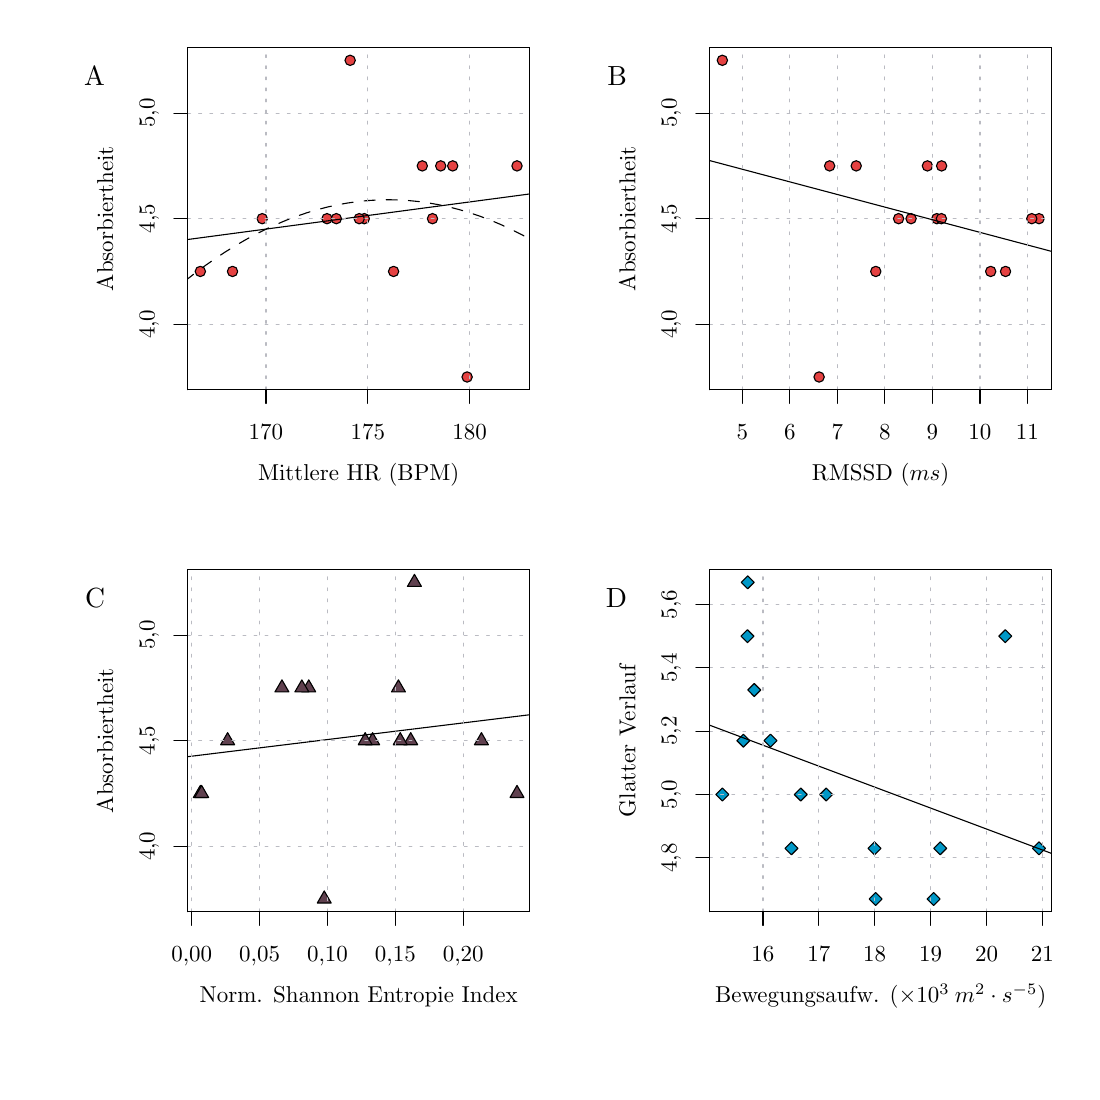
\begin{tikzpicture}[x=1pt,y=1pt]
\definecolor{fillColor}{RGB}{255,255,255}
\path[use as bounding box,fill=fillColor,fill opacity=0.00] (0,0) rectangle (377.25,377.25);
\begin{scope}
\path[clip] ( 57.82,246.44) rectangle (181.40,370.02);
\definecolor{drawColor}{RGB}{0,0,0}
\definecolor{fillColor}{RGB}{229,66,66}

\path[draw=drawColor,line width= 0.4pt,line join=round,line cap=round,fill=fillColor] ( 62.39,289.16) circle (  1.87);

\path[draw=drawColor,line width= 0.4pt,line join=round,line cap=round,fill=fillColor] ( 84.76,308.23) circle (  1.87);

\path[draw=drawColor,line width= 0.4pt,line join=round,line cap=round,fill=fillColor] ( 74.02,289.16) circle (  1.87);

\path[draw=drawColor,line width= 0.4pt,line join=round,line cap=round,fill=fillColor] (121.64,308.23) circle (  1.87);

\path[draw=drawColor,line width= 0.4pt,line join=round,line cap=round,fill=fillColor] (146.28,308.23) circle (  1.87);

\path[draw=drawColor,line width= 0.4pt,line join=round,line cap=round,fill=fillColor] (132.22,289.16) circle (  1.87);

\path[draw=drawColor,line width= 0.4pt,line join=round,line cap=round,fill=fillColor] (119.80,308.23) circle (  1.87);

\path[draw=drawColor,line width= 0.4pt,line join=round,line cap=round,fill=fillColor] (142.59,327.30) circle (  1.87);

\path[draw=drawColor,line width= 0.4pt,line join=round,line cap=round,fill=fillColor] (176.82,327.30) circle (  1.87);

\path[draw=drawColor,line width= 0.4pt,line join=round,line cap=round,fill=fillColor] (108.16,308.23) circle (  1.87);

\path[draw=drawColor,line width= 0.4pt,line join=round,line cap=round,fill=fillColor] (149.25,327.30) circle (  1.87);

\path[draw=drawColor,line width= 0.4pt,line join=round,line cap=round,fill=fillColor] (153.58,327.30) circle (  1.87);

\path[draw=drawColor,line width= 0.4pt,line join=round,line cap=round,fill=fillColor] (111.53,308.23) circle (  1.87);

\path[draw=drawColor,line width= 0.4pt,line join=round,line cap=round,fill=fillColor] (116.53,365.45) circle (  1.87);

\path[draw=drawColor,line width= 0.4pt,line join=round,line cap=round,fill=fillColor] (158.79,251.02) circle (  1.87);
\end{scope}
\begin{scope}
\path[clip] (  0.00,  0.00) rectangle (377.25,377.25);
\definecolor{drawColor}{RGB}{0,0,0}

\path[draw=drawColor,line width= 0.4pt,line join=round,line cap=round] ( 86.11,246.44) -- (159.71,246.44);

\path[draw=drawColor,line width= 0.4pt,line join=round,line cap=round] ( 86.11,246.44) -- ( 86.11,241.46);

\path[draw=drawColor,line width= 0.4pt,line join=round,line cap=round] (122.91,246.44) -- (122.91,241.46);

\path[draw=drawColor,line width= 0.4pt,line join=round,line cap=round] (159.71,246.44) -- (159.71,241.46);

\node[text=drawColor,anchor=base,inner sep=0pt, outer sep=0pt, scale=  0.83] at ( 86.11,228.51) {170};

\node[text=drawColor,anchor=base,inner sep=0pt, outer sep=0pt, scale=  0.83] at (122.91,228.51) {175};

\node[text=drawColor,anchor=base,inner sep=0pt, outer sep=0pt, scale=  0.83] at (159.71,228.51) {180};

\path[draw=drawColor,line width= 0.4pt,line join=round,line cap=round] ( 57.82,270.09) -- ( 57.82,346.37);

\path[draw=drawColor,line width= 0.4pt,line join=round,line cap=round] ( 57.82,270.09) -- ( 52.84,270.09);

\path[draw=drawColor,line width= 0.4pt,line join=round,line cap=round] ( 57.82,308.23) -- ( 52.84,308.23);

\path[draw=drawColor,line width= 0.4pt,line join=round,line cap=round] ( 57.82,346.37) -- ( 52.84,346.37);

\node[text=drawColor,rotate= 90.00,anchor=base,inner sep=0pt, outer sep=0pt, scale=  0.83] at ( 45.86,270.09) {4,0};

\node[text=drawColor,rotate= 90.00,anchor=base,inner sep=0pt, outer sep=0pt, scale=  0.83] at ( 45.86,308.23) {4,5};

\node[text=drawColor,rotate= 90.00,anchor=base,inner sep=0pt, outer sep=0pt, scale=  0.83] at ( 45.86,346.37) {5,0};

\path[draw=drawColor,line width= 0.4pt,line join=round,line cap=round] ( 57.82,246.44) --
	(181.40,246.44) --
	(181.40,370.02) --
	( 57.82,370.02) --
	( 57.82,246.44);
\end{scope}
\begin{scope}
\path[clip] (  0.00,188.62) rectangle (188.62,377.25);
\definecolor{drawColor}{RGB}{0,0,0}

\node[text=drawColor,anchor=base,inner sep=0pt, outer sep=0pt, scale=  0.83] at (119.61,213.57) {Mittlere HR (BPM)};

\node[text=drawColor,rotate= 90.00,anchor=base,inner sep=0pt, outer sep=0pt, scale=  0.83] at ( 30.92,308.23) {Absorbiertheit};
\end{scope}
\begin{scope}
\path[clip] ( 57.82,246.44) rectangle (181.40,370.02);
\definecolor{drawColor}{RGB}{0,0,0}

\path[draw=drawColor,line width= 0.4pt,line join=round,line cap=round] ( 57.82,300.70) -- (181.40,317.16);

\path[draw=drawColor,line width= 0.4pt,dash pattern=on 4pt off 4pt ,line join=round,line cap=round] ( 12.51,239.64) --
	( 16.19,244.27) --
	( 19.87,248.76) --
	( 23.55,253.11) --
	( 27.23,257.31) --
	( 30.91,261.35) --
	( 34.59,265.26) --
	( 38.27,269.01) --
	( 41.95,272.62) --
	( 45.63,276.08) --
	( 49.31,279.39) --
	( 52.99,282.56) --
	( 56.67,285.58) --
	( 60.35,288.45) --
	( 64.03,291.18) --
	( 67.71,293.76) --
	( 71.39,296.19) --
	( 75.07,298.47) --
	( 78.75,300.61) --
	( 82.43,302.60) --
	( 86.11,304.44) --
	( 89.79,306.13) --
	( 93.47,307.68) --
	( 97.15,309.08) --
	(100.83,310.34) --
	(104.51,311.44) --
	(108.19,312.40) --
	(111.87,313.21) --
	(115.55,313.88) --
	(119.23,314.40) --
	(122.91,314.77) --
	(126.59,314.99) --
	(130.27,315.07) --
	(133.95,315.00) --
	(137.63,314.78) --
	(141.31,314.41) --
	(144.99,313.90) --
	(148.67,313.24) --
	(152.35,312.44) --
	(156.03,311.48) --
	(159.71,310.38) --
	(163.39,309.13) --
	(167.07,307.74) --
	(170.75,306.20) --
	(174.43,304.51) --
	(178.11,302.67) --
	(181.79,300.69) --
	(185.47,298.56) --
	(189.15,296.28) --
	(192.83,293.85) --
	(196.51,291.28) --
	(200.19,288.56) --
	(203.87,285.70) --
	(207.55,282.68) --
	(211.23,279.52) --
	(214.91,276.21) --
	(218.59,272.76) --
	(222.27,269.16) --
	(225.95,265.41) --
	(229.63,261.51) --
	(233.31,257.47);
\definecolor{drawColor}{RGB}{186,187,194}

\path[draw=drawColor,line width= 0.4pt,dash pattern=on 1pt off 3pt ,line join=round,line cap=round] ( 86.11,246.44) -- ( 86.11,370.02);

\path[draw=drawColor,line width= 0.4pt,dash pattern=on 1pt off 3pt ,line join=round,line cap=round] (122.91,246.44) -- (122.91,370.02);

\path[draw=drawColor,line width= 0.4pt,dash pattern=on 1pt off 3pt ,line join=round,line cap=round] (159.71,246.44) -- (159.71,370.02);

\path[draw=drawColor,line width= 0.4pt,dash pattern=on 1pt off 3pt ,line join=round,line cap=round] ( 57.82,270.09) -- (181.40,270.09);

\path[draw=drawColor,line width= 0.4pt,dash pattern=on 1pt off 3pt ,line join=round,line cap=round] ( 57.82,308.23) -- (181.40,308.23);

\path[draw=drawColor,line width= 0.4pt,dash pattern=on 1pt off 3pt ,line join=round,line cap=round] ( 57.82,346.37) -- (181.40,346.37);
\end{scope}
\begin{scope}
\path[clip] (  0.00,  0.00) rectangle (377.25,377.25);
\definecolor{drawColor}{RGB}{0,0,0}

\path[draw=drawColor,line width= 0.4pt,line join=round,line cap=round] ( 57.82,246.44) --
	(181.40,246.44) --
	(181.40,370.02) --
	( 57.82,370.02) --
	( 57.82,246.44);

\node[text=drawColor,anchor=base east,inner sep=0pt, outer sep=0pt, scale=  1.00] at ( 27.94,356.44) {A};
\end{scope}
\begin{scope}
\path[clip] (246.44,246.44) rectangle (370.02,370.02);
\definecolor{drawColor}{RGB}{0,0,0}
\definecolor{fillColor}{RGB}{229,66,66}

\path[draw=drawColor,line width= 0.4pt,line join=round,line cap=round,fill=fillColor] (347.99,289.16) circle (  1.87);

\path[draw=drawColor,line width= 0.4pt,line join=round,line cap=round,fill=fillColor] (328.51,308.23) circle (  1.87);

\path[draw=drawColor,line width= 0.4pt,line join=round,line cap=round,fill=fillColor] (306.46,289.16) circle (  1.87);

\path[draw=drawColor,line width= 0.4pt,line join=round,line cap=round,fill=fillColor] (365.45,308.23) circle (  1.87);

\path[draw=drawColor,line width= 0.4pt,line join=round,line cap=round,fill=fillColor] (362.83,308.23) circle (  1.87);

\path[draw=drawColor,line width= 0.4pt,line join=round,line cap=round,fill=fillColor] (353.35,289.16) circle (  1.87);

\path[draw=drawColor,line width= 0.4pt,line join=round,line cap=round,fill=fillColor] (330.17,308.23) circle (  1.87);

\path[draw=drawColor,line width= 0.4pt,line join=round,line cap=round,fill=fillColor] (325.12,327.30) circle (  1.87);

\path[draw=drawColor,line width= 0.4pt,line join=round,line cap=round,fill=fillColor] (330.25,327.30) circle (  1.87);

\path[draw=drawColor,line width= 0.4pt,line join=round,line cap=round,fill=fillColor] (314.70,308.23) circle (  1.87);

\path[draw=drawColor,line width= 0.4pt,line join=round,line cap=round,fill=fillColor] (299.39,327.30) circle (  1.87);

\path[draw=drawColor,line width= 0.4pt,line join=round,line cap=round,fill=fillColor] (289.79,327.30) circle (  1.87);

\path[draw=drawColor,line width= 0.4pt,line join=round,line cap=round,fill=fillColor] (319.21,308.23) circle (  1.87);

\path[draw=drawColor,line width= 0.4pt,line join=round,line cap=round,fill=fillColor] (251.02,365.45) circle (  1.87);

\path[draw=drawColor,line width= 0.4pt,line join=round,line cap=round,fill=fillColor] (285.98,251.02) circle (  1.87);
\end{scope}
\begin{scope}
\path[clip] (  0.00,  0.00) rectangle (377.25,377.25);
\definecolor{drawColor}{RGB}{0,0,0}

\path[draw=drawColor,line width= 0.4pt,line join=round,line cap=round] (258.28,246.44) -- (361.26,246.44);

\path[draw=drawColor,line width= 0.4pt,line join=round,line cap=round] (258.28,246.44) -- (258.28,241.46);

\path[draw=drawColor,line width= 0.4pt,line join=round,line cap=round] (275.44,246.44) -- (275.44,241.46);

\path[draw=drawColor,line width= 0.4pt,line join=round,line cap=round] (292.61,246.44) -- (292.61,241.46);

\path[draw=drawColor,line width= 0.4pt,line join=round,line cap=round] (309.77,246.44) -- (309.77,241.46);

\path[draw=drawColor,line width= 0.4pt,line join=round,line cap=round] (326.93,246.44) -- (326.93,241.46);

\path[draw=drawColor,line width= 0.4pt,line join=round,line cap=round] (344.10,246.44) -- (344.10,241.46);

\path[draw=drawColor,line width= 0.4pt,line join=round,line cap=round] (361.26,246.44) -- (361.26,241.46);

\node[text=drawColor,anchor=base,inner sep=0pt, outer sep=0pt, scale=  0.83] at (258.28,228.51) {5};

\node[text=drawColor,anchor=base,inner sep=0pt, outer sep=0pt, scale=  0.83] at (275.44,228.51) {6};

\node[text=drawColor,anchor=base,inner sep=0pt, outer sep=0pt, scale=  0.83] at (292.61,228.51) {7};

\node[text=drawColor,anchor=base,inner sep=0pt, outer sep=0pt, scale=  0.83] at (309.77,228.51) {8};

\node[text=drawColor,anchor=base,inner sep=0pt, outer sep=0pt, scale=  0.83] at (326.93,228.51) {9};

\node[text=drawColor,anchor=base,inner sep=0pt, outer sep=0pt, scale=  0.83] at (344.10,228.51) {10};

\node[text=drawColor,anchor=base,inner sep=0pt, outer sep=0pt, scale=  0.83] at (361.26,228.51) {11};

\path[draw=drawColor,line width= 0.4pt,line join=round,line cap=round] (246.44,270.09) -- (246.44,346.37);

\path[draw=drawColor,line width= 0.4pt,line join=round,line cap=round] (246.44,270.09) -- (241.46,270.09);

\path[draw=drawColor,line width= 0.4pt,line join=round,line cap=round] (246.44,308.23) -- (241.46,308.23);

\path[draw=drawColor,line width= 0.4pt,line join=round,line cap=round] (246.44,346.37) -- (241.46,346.37);

\node[text=drawColor,rotate= 90.00,anchor=base,inner sep=0pt, outer sep=0pt, scale=  0.83] at (234.49,270.09) {4,0};

\node[text=drawColor,rotate= 90.00,anchor=base,inner sep=0pt, outer sep=0pt, scale=  0.83] at (234.49,308.23) {4,5};

\node[text=drawColor,rotate= 90.00,anchor=base,inner sep=0pt, outer sep=0pt, scale=  0.83] at (234.49,346.37) {5,0};

\path[draw=drawColor,line width= 0.4pt,line join=round,line cap=round] (246.44,246.44) --
	(370.02,246.44) --
	(370.02,370.02) --
	(246.44,370.02) --
	(246.44,246.44);
\end{scope}
\begin{scope}
\path[clip] (188.62,188.62) rectangle (377.25,377.25);
\definecolor{drawColor}{RGB}{0,0,0}

\node[text=drawColor,anchor=base,inner sep=0pt, outer sep=0pt, scale=  0.83] at (308.23,213.57) {RMSSD ($ms$)};

\node[text=drawColor,rotate= 90.00,anchor=base,inner sep=0pt, outer sep=0pt, scale=  0.83] at (219.55,308.23) {Absorbiertheit};
\end{scope}
\begin{scope}
\path[clip] (246.44,246.44) rectangle (370.02,370.02);
\definecolor{drawColor}{RGB}{0,0,0}

\path[draw=drawColor,line width= 0.4pt,line join=round,line cap=round] (246.44,329.22) -- (370.02,296.40);
\definecolor{drawColor}{RGB}{186,187,194}

\path[draw=drawColor,line width= 0.4pt,dash pattern=on 1pt off 3pt ,line join=round,line cap=round] (258.28,246.44) -- (258.28,370.02);

\path[draw=drawColor,line width= 0.4pt,dash pattern=on 1pt off 3pt ,line join=round,line cap=round] (275.44,246.44) -- (275.44,370.02);

\path[draw=drawColor,line width= 0.4pt,dash pattern=on 1pt off 3pt ,line join=round,line cap=round] (292.61,246.44) -- (292.61,370.02);

\path[draw=drawColor,line width= 0.4pt,dash pattern=on 1pt off 3pt ,line join=round,line cap=round] (309.77,246.44) -- (309.77,370.02);

\path[draw=drawColor,line width= 0.4pt,dash pattern=on 1pt off 3pt ,line join=round,line cap=round] (326.93,246.44) -- (326.93,370.02);

\path[draw=drawColor,line width= 0.4pt,dash pattern=on 1pt off 3pt ,line join=round,line cap=round] (344.10,246.44) -- (344.10,370.02);

\path[draw=drawColor,line width= 0.4pt,dash pattern=on 1pt off 3pt ,line join=round,line cap=round] (361.26,246.44) -- (361.26,370.02);

\path[draw=drawColor,line width= 0.4pt,dash pattern=on 1pt off 3pt ,line join=round,line cap=round] (246.44,270.09) -- (370.02,270.09);

\path[draw=drawColor,line width= 0.4pt,dash pattern=on 1pt off 3pt ,line join=round,line cap=round] (246.44,308.23) -- (370.02,308.23);

\path[draw=drawColor,line width= 0.4pt,dash pattern=on 1pt off 3pt ,line join=round,line cap=round] (246.44,346.37) -- (370.02,346.37);
\end{scope}
\begin{scope}
\path[clip] (  0.00,  0.00) rectangle (377.25,377.25);
\definecolor{drawColor}{RGB}{0,0,0}

\path[draw=drawColor,line width= 0.4pt,line join=round,line cap=round] (246.44,246.44) --
	(370.02,246.44) --
	(370.02,370.02) --
	(246.44,370.02) --
	(246.44,246.44);

\node[text=drawColor,anchor=base east,inner sep=0pt, outer sep=0pt, scale=  1.00] at (216.56,356.44) {B};
\end{scope}
\begin{scope}
\path[clip] ( 57.82, 57.82) rectangle (181.40,181.40);
\definecolor{drawColor}{RGB}{0,0,0}
\definecolor{fillColor}{RGB}{96,65,79}

\path[draw=drawColor,line width= 0.4pt,line join=round,line cap=round,fill=fillColor] ( 62.39,103.44) --
	( 64.91, 99.08) --
	( 59.88, 99.08) --
	cycle;

\path[draw=drawColor,line width= 0.4pt,line join=round,line cap=round,fill=fillColor] ( 72.25,122.51) --
	( 74.77,118.15) --
	( 69.74,118.15) --
	cycle;

\path[draw=drawColor,line width= 0.4pt,line join=round,line cap=round,fill=fillColor] ( 62.87,103.44) --
	( 65.38, 99.08) --
	( 60.35, 99.08) --
	cycle;

\path[draw=drawColor,line width= 0.4pt,line join=round,line cap=round,fill=fillColor] (163.97,122.51) --
	(166.48,118.15) --
	(161.45,118.15) --
	cycle;

\path[draw=drawColor,line width= 0.4pt,line join=round,line cap=round,fill=fillColor] (138.41,122.51) --
	(140.92,118.15) --
	(135.89,118.15) --
	cycle;

\path[draw=drawColor,line width= 0.4pt,line join=round,line cap=round,fill=fillColor] (176.82,103.44) --
	(179.34, 99.08) --
	(174.31, 99.08) --
	cycle;

\path[draw=drawColor,line width= 0.4pt,line join=round,line cap=round,fill=fillColor] (134.62,122.51) --
	(137.14,118.15) --
	(132.10,118.15) --
	cycle;

\path[draw=drawColor,line width= 0.4pt,line join=round,line cap=round,fill=fillColor] (133.97,141.58) --
	(136.49,137.23) --
	(131.46,137.23) --
	cycle;

\path[draw=drawColor,line width= 0.4pt,line join=round,line cap=round,fill=fillColor] (101.57,141.58) --
	(104.08,137.23) --
	( 99.05,137.23) --
	cycle;

\path[draw=drawColor,line width= 0.4pt,line join=round,line cap=round,fill=fillColor] (124.65,122.51) --
	(127.16,118.15) --
	(122.13,118.15) --
	cycle;

\path[draw=drawColor,line width= 0.4pt,line join=round,line cap=round,fill=fillColor] ( 99.07,141.58) --
	(101.59,137.23) --
	( 96.56,137.23) --
	cycle;

\path[draw=drawColor,line width= 0.4pt,line join=round,line cap=round,fill=fillColor] ( 91.88,141.58) --
	( 94.39,137.23) --
	( 89.36,137.23) --
	cycle;

\path[draw=drawColor,line width= 0.4pt,line join=round,line cap=round,fill=fillColor] (121.96,122.51) --
	(124.48,118.15) --
	(119.45,118.15) --
	cycle;

\path[draw=drawColor,line width= 0.4pt,line join=round,line cap=round,fill=fillColor] (139.76,179.72) --
	(142.27,175.37) --
	(137.24,175.37) --
	cycle;

\path[draw=drawColor,line width= 0.4pt,line join=round,line cap=round,fill=fillColor] (107.17, 65.30) --
	(109.68, 60.94) --
	(104.65, 60.94) --
	cycle;
\end{scope}
\begin{scope}
\path[clip] (  0.00,  0.00) rectangle (377.25,377.25);
\definecolor{drawColor}{RGB}{0,0,0}

\path[draw=drawColor,line width= 0.4pt,line join=round,line cap=round] ( 59.27, 57.82) -- (157.41, 57.82);

\path[draw=drawColor,line width= 0.4pt,line join=round,line cap=round] ( 59.27, 57.82) -- ( 59.27, 52.84);

\path[draw=drawColor,line width= 0.4pt,line join=round,line cap=round] ( 83.81, 57.82) -- ( 83.81, 52.84);

\path[draw=drawColor,line width= 0.4pt,line join=round,line cap=round] (108.34, 57.82) -- (108.34, 52.84);

\path[draw=drawColor,line width= 0.4pt,line join=round,line cap=round] (132.88, 57.82) -- (132.88, 52.84);

\path[draw=drawColor,line width= 0.4pt,line join=round,line cap=round] (157.41, 57.82) -- (157.41, 52.84);

\node[text=drawColor,anchor=base,inner sep=0pt, outer sep=0pt, scale=  0.83] at ( 59.27, 39.89) {0,00};

\node[text=drawColor,anchor=base,inner sep=0pt, outer sep=0pt, scale=  0.83] at ( 83.81, 39.89) {0,05};

\node[text=drawColor,anchor=base,inner sep=0pt, outer sep=0pt, scale=  0.83] at (108.34, 39.89) {0,10};

\node[text=drawColor,anchor=base,inner sep=0pt, outer sep=0pt, scale=  0.83] at (132.88, 39.89) {0,15};

\node[text=drawColor,anchor=base,inner sep=0pt, outer sep=0pt, scale=  0.83] at (157.41, 39.89) {0,20};

\path[draw=drawColor,line width= 0.4pt,line join=round,line cap=round] ( 57.82, 81.46) -- ( 57.82,157.75);

\path[draw=drawColor,line width= 0.4pt,line join=round,line cap=round] ( 57.82, 81.46) -- ( 52.84, 81.46);

\path[draw=drawColor,line width= 0.4pt,line join=round,line cap=round] ( 57.82,119.61) -- ( 52.84,119.61);

\path[draw=drawColor,line width= 0.4pt,line join=round,line cap=round] ( 57.82,157.75) -- ( 52.84,157.75);

\node[text=drawColor,rotate= 90.00,anchor=base,inner sep=0pt, outer sep=0pt, scale=  0.83] at ( 45.86, 81.46) {4,0};

\node[text=drawColor,rotate= 90.00,anchor=base,inner sep=0pt, outer sep=0pt, scale=  0.83] at ( 45.86,119.61) {4,5};

\node[text=drawColor,rotate= 90.00,anchor=base,inner sep=0pt, outer sep=0pt, scale=  0.83] at ( 45.86,157.75) {5,0};

\path[draw=drawColor,line width= 0.4pt,line join=round,line cap=round] ( 57.82, 57.82) --
	(181.40, 57.82) --
	(181.40,181.40) --
	( 57.82,181.40) --
	( 57.82, 57.82);
\end{scope}
\begin{scope}
\path[clip] (  0.00,  0.00) rectangle (188.62,188.62);
\definecolor{drawColor}{RGB}{0,0,0}

\node[text=drawColor,anchor=base,inner sep=0pt, outer sep=0pt, scale=  0.83] at (119.61, 24.95) {Norm. Shannon Entropie Index};

\node[text=drawColor,rotate= 90.00,anchor=base,inner sep=0pt, outer sep=0pt, scale=  0.83] at ( 30.92,119.61) {Absorbiertheit};
\end{scope}
\begin{scope}
\path[clip] ( 57.82, 57.82) rectangle (181.40,181.40);
\definecolor{drawColor}{RGB}{0,0,0}

\path[draw=drawColor,line width= 0.4pt,line join=round,line cap=round] ( 57.82,113.82) -- (181.40,128.97);
\definecolor{drawColor}{RGB}{186,187,194}

\path[draw=drawColor,line width= 0.4pt,dash pattern=on 1pt off 3pt ,line join=round,line cap=round] ( 59.27, 57.82) -- ( 59.27,181.40);

\path[draw=drawColor,line width= 0.4pt,dash pattern=on 1pt off 3pt ,line join=round,line cap=round] ( 83.81, 57.82) -- ( 83.81,181.40);

\path[draw=drawColor,line width= 0.4pt,dash pattern=on 1pt off 3pt ,line join=round,line cap=round] (108.34, 57.82) -- (108.34,181.40);

\path[draw=drawColor,line width= 0.4pt,dash pattern=on 1pt off 3pt ,line join=round,line cap=round] (132.88, 57.82) -- (132.88,181.40);

\path[draw=drawColor,line width= 0.4pt,dash pattern=on 1pt off 3pt ,line join=round,line cap=round] (157.41, 57.82) -- (157.41,181.40);

\path[draw=drawColor,line width= 0.4pt,dash pattern=on 1pt off 3pt ,line join=round,line cap=round] ( 57.82, 81.46) -- (181.40, 81.46);

\path[draw=drawColor,line width= 0.4pt,dash pattern=on 1pt off 3pt ,line join=round,line cap=round] ( 57.82,119.61) -- (181.40,119.61);

\path[draw=drawColor,line width= 0.4pt,dash pattern=on 1pt off 3pt ,line join=round,line cap=round] ( 57.82,157.75) -- (181.40,157.75);
\end{scope}
\begin{scope}
\path[clip] (  0.00,  0.00) rectangle (377.25,377.25);
\definecolor{drawColor}{RGB}{0,0,0}

\path[draw=drawColor,line width= 0.4pt,line join=round,line cap=round] ( 57.82, 57.82) --
	(181.40, 57.82) --
	(181.40,181.40) --
	( 57.82,181.40) --
	( 57.82, 57.82);

\node[text=drawColor,anchor=base east,inner sep=0pt, outer sep=0pt, scale=  1.00] at ( 27.94,167.82) {C};
\end{scope}
\begin{scope}
\path[clip] (246.44, 57.82) rectangle (370.02,181.40);
\definecolor{drawColor}{RGB}{0,0,0}
\definecolor{fillColor}{RGB}{0,152,199}

\path[draw=drawColor,line width= 0.4pt,line join=round,line cap=round,fill=fillColor] (306.00, 78.36) --
	(308.34, 80.70) --
	(306.00, 83.04) --
	(303.66, 80.70) --
	cycle;

\path[draw=drawColor,line width= 0.4pt,line join=round,line cap=round,fill=fillColor] (306.40, 60.05) --
	(308.74, 62.39) --
	(306.40, 64.73) --
	(304.06, 62.39) --
	cycle;

\path[draw=drawColor,line width= 0.4pt,line join=round,line cap=round,fill=fillColor] (327.35, 60.05) --
	(329.69, 62.39) --
	(327.35, 64.73) --
	(325.01, 62.39) --
	cycle;

\path[draw=drawColor,line width= 0.4pt,line join=round,line cap=round,fill=fillColor] (279.35, 97.81) --
	(281.69,100.15) --
	(279.35,102.49) --
	(277.01,100.15) --
	cycle;

\path[draw=drawColor,line width= 0.4pt,line join=round,line cap=round,fill=fillColor] (288.55, 97.81) --
	(290.89,100.15) --
	(288.55,102.49) --
	(286.21,100.15) --
	cycle;

\path[draw=drawColor,line width= 0.4pt,line join=round,line cap=round,fill=fillColor] (275.99, 78.36) --
	(278.33, 80.70) --
	(275.99, 83.04) --
	(273.65, 80.70) --
	cycle;

\path[draw=drawColor,line width= 0.4pt,line join=round,line cap=round,fill=fillColor] (251.02, 97.81) --
	(253.36,100.15) --
	(251.02,102.49) --
	(248.68,100.15) --
	cycle;

\path[draw=drawColor,line width= 0.4pt,line join=round,line cap=round,fill=fillColor] (260.08,155.03) --
	(262.42,157.37) --
	(260.08,159.71) --
	(257.74,157.37) --
	cycle;

\path[draw=drawColor,line width= 0.4pt,line join=round,line cap=round,fill=fillColor] (268.42,117.27) --
	(270.76,119.61) --
	(268.42,121.95) --
	(266.08,119.61) --
	cycle;

\path[draw=drawColor,line width= 0.4pt,line join=round,line cap=round,fill=fillColor] (258.61,117.27) --
	(260.95,119.61) --
	(258.61,121.95) --
	(256.27,119.61) --
	cycle;

\path[draw=drawColor,line width= 0.4pt,line join=round,line cap=round,fill=fillColor] (262.55,135.57) --
	(264.89,137.92) --
	(262.55,140.26) --
	(260.21,137.92) --
	cycle;

\path[draw=drawColor,line width= 0.4pt,line join=round,line cap=round,fill=fillColor] (260.17,174.48) --
	(262.51,176.82) --
	(260.17,179.16) --
	(257.83,176.82) --
	cycle;

\path[draw=drawColor,line width= 0.4pt,line join=round,line cap=round,fill=fillColor] (353.27,155.03) --
	(355.61,157.37) --
	(353.27,159.71) --
	(350.93,157.37) --
	cycle;

\path[draw=drawColor,line width= 0.4pt,line join=round,line cap=round,fill=fillColor] (329.74, 78.36) --
	(332.08, 80.70) --
	(329.74, 83.04) --
	(327.40, 80.70) --
	cycle;

\path[draw=drawColor,line width= 0.4pt,line join=round,line cap=round,fill=fillColor] (365.45, 78.36) --
	(367.79, 80.70) --
	(365.45, 83.04) --
	(363.10, 80.70) --
	cycle;
\end{scope}
\begin{scope}
\path[clip] (  0.00,  0.00) rectangle (377.25,377.25);
\definecolor{drawColor}{RGB}{0,0,0}

\path[draw=drawColor,line width= 0.4pt,line join=round,line cap=round] (265.69, 57.82) -- (366.68, 57.82);

\path[draw=drawColor,line width= 0.4pt,line join=round,line cap=round] (265.69, 57.82) -- (265.69, 52.84);

\path[draw=drawColor,line width= 0.4pt,line join=round,line cap=round] (285.89, 57.82) -- (285.89, 52.84);

\path[draw=drawColor,line width= 0.4pt,line join=round,line cap=round] (306.08, 57.82) -- (306.08, 52.84);

\path[draw=drawColor,line width= 0.4pt,line join=round,line cap=round] (326.28, 57.82) -- (326.28, 52.84);

\path[draw=drawColor,line width= 0.4pt,line join=round,line cap=round] (346.48, 57.82) -- (346.48, 52.84);

\path[draw=drawColor,line width= 0.4pt,line join=round,line cap=round] (366.68, 57.82) -- (366.68, 52.84);

\node[text=drawColor,anchor=base,inner sep=0pt, outer sep=0pt, scale=  0.83] at (265.69, 39.89) {16};

\node[text=drawColor,anchor=base,inner sep=0pt, outer sep=0pt, scale=  0.83] at (285.89, 39.89) {17};

\node[text=drawColor,anchor=base,inner sep=0pt, outer sep=0pt, scale=  0.83] at (306.08, 39.89) {18};

\node[text=drawColor,anchor=base,inner sep=0pt, outer sep=0pt, scale=  0.83] at (326.28, 39.89) {19};

\node[text=drawColor,anchor=base,inner sep=0pt, outer sep=0pt, scale=  0.83] at (346.48, 39.89) {20};

\node[text=drawColor,anchor=base,inner sep=0pt, outer sep=0pt, scale=  0.83] at (366.68, 39.89) {21};

\path[draw=drawColor,line width= 0.4pt,line join=round,line cap=round] (246.44, 77.27) -- (246.44,168.81);

\path[draw=drawColor,line width= 0.4pt,line join=round,line cap=round] (246.44, 77.27) -- (241.46, 77.27);

\path[draw=drawColor,line width= 0.4pt,line join=round,line cap=round] (246.44,100.15) -- (241.46,100.15);

\path[draw=drawColor,line width= 0.4pt,line join=round,line cap=round] (246.44,123.04) -- (241.46,123.04);

\path[draw=drawColor,line width= 0.4pt,line join=round,line cap=round] (246.44,145.93) -- (241.46,145.93);

\path[draw=drawColor,line width= 0.4pt,line join=round,line cap=round] (246.44,168.81) -- (241.46,168.81);

\node[text=drawColor,rotate= 90.00,anchor=base,inner sep=0pt, outer sep=0pt, scale=  0.83] at (234.49, 77.27) {4,8};

\node[text=drawColor,rotate= 90.00,anchor=base,inner sep=0pt, outer sep=0pt, scale=  0.83] at (234.49,100.15) {5,0};

\node[text=drawColor,rotate= 90.00,anchor=base,inner sep=0pt, outer sep=0pt, scale=  0.83] at (234.49,123.04) {5,2};

\node[text=drawColor,rotate= 90.00,anchor=base,inner sep=0pt, outer sep=0pt, scale=  0.83] at (234.49,145.93) {5,4};

\node[text=drawColor,rotate= 90.00,anchor=base,inner sep=0pt, outer sep=0pt, scale=  0.83] at (234.49,168.81) {5,6};

\path[draw=drawColor,line width= 0.4pt,line join=round,line cap=round] (246.44, 57.82) --
	(370.02, 57.82) --
	(370.02,181.40) --
	(246.44,181.40) --
	(246.44, 57.82);
\end{scope}
\begin{scope}
\path[clip] (188.62,  0.00) rectangle (377.25,188.62);
\definecolor{drawColor}{RGB}{0,0,0}

\node[text=drawColor,anchor=base,inner sep=0pt, outer sep=0pt, scale=  0.83] at (308.23, 24.95) {Bewegungsaufw. ($\times 10^3 \: m^2 \cdot s^{-5}$)};

\node[text=drawColor,rotate= 90.00,anchor=base,inner sep=0pt, outer sep=0pt, scale=  0.83] at (219.55,119.61) {Glatter Verlauf};
\end{scope}
\begin{scope}
\path[clip] (246.44, 57.82) rectangle (370.02,181.40);
\definecolor{drawColor}{RGB}{0,0,0}

\path[draw=drawColor,line width= 0.4pt,line join=round,line cap=round] (246.44,125.19) -- (370.02, 78.85);
\definecolor{drawColor}{RGB}{186,187,194}

\path[draw=drawColor,line width= 0.4pt,dash pattern=on 1pt off 3pt ,line join=round,line cap=round] (265.69, 57.82) -- (265.69,181.40);

\path[draw=drawColor,line width= 0.4pt,dash pattern=on 1pt off 3pt ,line join=round,line cap=round] (285.89, 57.82) -- (285.89,181.40);

\path[draw=drawColor,line width= 0.4pt,dash pattern=on 1pt off 3pt ,line join=round,line cap=round] (306.08, 57.82) -- (306.08,181.40);

\path[draw=drawColor,line width= 0.4pt,dash pattern=on 1pt off 3pt ,line join=round,line cap=round] (326.28, 57.82) -- (326.28,181.40);

\path[draw=drawColor,line width= 0.4pt,dash pattern=on 1pt off 3pt ,line join=round,line cap=round] (346.48, 57.82) -- (346.48,181.40);

\path[draw=drawColor,line width= 0.4pt,dash pattern=on 1pt off 3pt ,line join=round,line cap=round] (366.68, 57.82) -- (366.68,181.40);

\path[draw=drawColor,line width= 0.4pt,dash pattern=on 1pt off 3pt ,line join=round,line cap=round] (246.44, 77.27) -- (370.02, 77.27);

\path[draw=drawColor,line width= 0.4pt,dash pattern=on 1pt off 3pt ,line join=round,line cap=round] (246.44,100.15) -- (370.02,100.15);

\path[draw=drawColor,line width= 0.4pt,dash pattern=on 1pt off 3pt ,line join=round,line cap=round] (246.44,123.04) -- (370.02,123.04);

\path[draw=drawColor,line width= 0.4pt,dash pattern=on 1pt off 3pt ,line join=round,line cap=round] (246.44,145.93) -- (370.02,145.93);

\path[draw=drawColor,line width= 0.4pt,dash pattern=on 1pt off 3pt ,line join=round,line cap=round] (246.44,168.81) -- (370.02,168.81);
\end{scope}
\begin{scope}
\path[clip] (  0.00,  0.00) rectangle (377.25,377.25);
\definecolor{drawColor}{RGB}{0,0,0}

\path[draw=drawColor,line width= 0.4pt,line join=round,line cap=round] (246.44, 57.82) --
	(370.02, 57.82) --
	(370.02,181.40) --
	(246.44,181.40) --
	(246.44, 57.82);

\node[text=drawColor,anchor=base east,inner sep=0pt, outer sep=0pt, scale=  1.00] at (216.56,167.82) {D};
\end{scope}
\end{tikzpicture}

	\caption[Beobachtungen der Fallstudie zum Flow-Erleben beim Laufen]{Beobachtungen der Fallstudie zum Flow-Erleben beim Laufen. (A) Absorbiertheit und mittlerer HR; (B) Absorbiertheit und RMSSD; (C) Absorbiertheit und mittlerer normalisierter Shannon Entropie Index; (D) Glatter Verlauf und mittlerer Bewegungsaufwand. Quelle: Eigene Darstellung \\ \hspace{\textwidth}\emph{Anmerkung}: Durchgezogene Linie stellt das bestmögliche liniare Modell dar. \\ \hspace{\textwidth}Gestrichelte Linie stellt ggf. das bestmögliche quardratische Modell dar.}
	\label{fig:5_8_regression}
\end{figure}

\subsubsection{Prozessorientierter Ansatz}
\label{subs:prozessorientierter_ansatz_1}
Aus der Motivation heraus Flow-Erleben prozessorientiert zu messen, begutachtete ich die Zeitreihen der Kandidaten zur impliziten Flow-Erfassung visuell. Ich probierte unterschiedliche Software zur Visualisierung von zeitbasierten multimodalen Daten wie den \emph{Observer XT} von \emph{Noldus} aus. Der \emph{Observer} ist ein Werkzeug, das die parallele Untersuchung von mehreren Datenströmen in der Zeit und mit Bezug auf den geografischen Raum ermöglicht. Den Bezug zum geografischen Raum stellt der \emph{Observer} über eine zweite Software namens \emph{Tracklab} her. Der \emph{Observer} ermöglicht die Annotation der Daten, um konkrete Zeiträume bzw. Phasen genauer durch verändern des Zoomfaktors zu betrachten. Leider ist der Import von Daten in den \emph{Observer} und in \emph{Tracklab} aufwendig. Für beide Programme braucht man teure Lizenzen und die Nutzbarkeit ist für unseren Verwendungszweck nicht befriedigend.

Ein freies Programm namens \emph{ChronoViz} \citep{Fouse2010, Fouse2011}, welches die Visualisierung von mehreren Datenströmen in Bezug auf einen geografischen Raum ermöglicht, war nicht in der Lage die Menge an Daten zu verarbeiten. Daraus folgt, dass ein benutzerfreundliches Werkzeug, dass eine prozessorientierte Untersuchung mit Bezug auf einen geografischen Raum im Bereich der Mensch-Computer-Interaktion fehlt.

Als Konsequenz nutzte ich zur Visualisierung der Datenströme \emph{R} und zur Visualisierung der geographischen Daten \emph{Google Earth}, auch wenn ich das Zoomen in die Daten und die Synchronisation der Zeit zwischen Datenpunkt und geografischer Position per Hand vornehmen musste.

Im Rahmen der graphischen Analyse stellte ich unterschiedliche Zeitreihen gegenüber, u. a. Zeitreihen mit Unterforderung, Überforderung und optimalen Läufen. In der Auswahl von Zeitabschnitten (300 Sekunden vor der Selbstauskunft) in Abbildung~\ref{fig:5_9_prozessorientierter_ansatz} ist der Einfluss der Belastung auf die Absorbiertheit als Kernmerkmal für Flow-Erleben und auf die potentiellen Kandidaten zur impliziten Flow-Messung zu erkennen. Eine Unterforderung ist in Abbildung~\ref{fig:5_9_prozessorientierter_ansatz} links dargestellt. Mit einem Wert der Absorbiertheit von 4,25 besitzt der Laufabschnitt einen durchschnittlichen Wert gegenüber den restlichen Laufabschnitten. Die mittlere \ac{HR} liegt auf einem unteren Niveau für die Untersuchungsperson. Ihre Varianz ist höher als in den anderen beiden Zeitabschnitten in der Auswahl. Durch die niedrige mittlere \ac{HR} kommt es zu keiner kardio-lokomotorischen Phasensynchronisation. Im Synchrogramm wandern die zwei Herzschläge pro Bewegungsablauf nach oben. Der Bewegungsaufwand ist durch die niedrigere Geschwindigkeit geringer als in den anderen beiden Zeitabschnitten in der Auswahl.

Ein optimaler Lauf ist in der Mitte von Abbildung~\ref{fig:5_9_prozessorientierter_ansatz} dargestellt. In der Studie ist es der Lauf mit dem höchsten Wert von Absorbiertheit. Die Untersuchungsperson besitzt eine konstante mittlere \ac{HR} von 174 Schlägen pro Minute. Die konstante mittlere \ac{HR} lässt sich nicht unbedingt aus der Laufgeschwindigkeit herleiten, auch wenn der Bewegungsaufwand im Zeitabschnitt und dessen Varianz niedriger ist. Zusätzlich könnte eine optimale Atmung die konstante mittlere \ac{HR} auslösen. Die konstante mittlere \ac{HR} von 174 Schlägen pro Minute führt bei der Untersuchungsperson zu einer kardio-lokomotorischen Phasensynchronisation. Die kardio-lokomotorische Phasensynchronisation stellt sich im Synchrogramm als zwei waagerechte Linien dar.

Eine Überforderung ist rechts in Abbildung~\ref{fig:5_9_prozessorientierter_ansatz} dargestellt. Der Wert der Absorbiertheit des Zeitabschnitts ist mit 3,75 der Niedrigste aller Bewertungen der Untersuchungsperson. Die mittlere \ac{HR} ist erheblich höher als in den anderen beiden Zeitabschnitten. Der Bewegungsaufwand ist wegen der größeren Geschwindigkeit bis zur 3360 Sekunde erhöht. Danach verringerte die Untersuchungsperson die Geschwindigkeit. Die mittlere \ac{HR} zeigt keine sofortige Anpassung, aber an der relativen Phase der kardio-lokomotorischen Phasensynchronisation ist der Geschwindigkeitsunterschied durch den Musterwechsel zu erkennen. Die Überforderung führt zu keiner Phasensynchronisation. Im Synchrogramm wandern die zwei Herzschläge pro Bewegungsablauf nach unten.

\begin{sidewaysfigure}
	\resizebox{1.00\textwidth}{!}{%
		% Created by tikzDevice version 0.10.1 on 2016-06-15 07:22:33
% !TEX encoding = UTF-8 Unicode
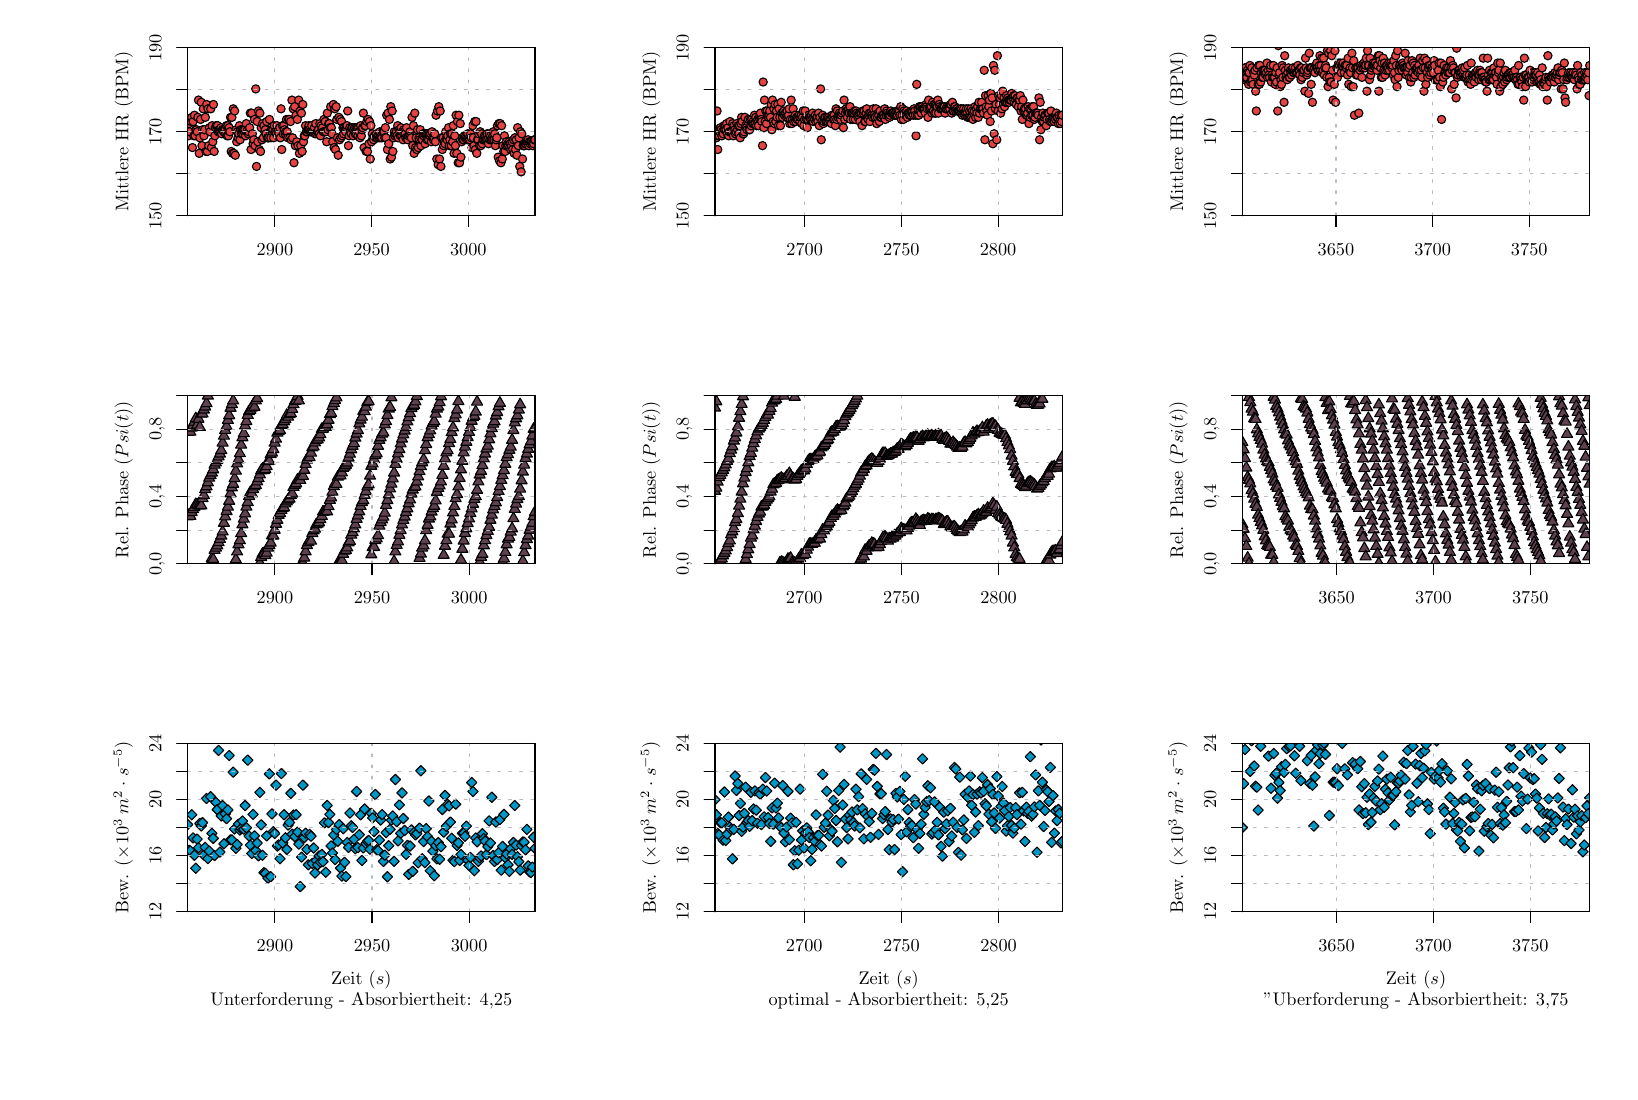
\begin{tikzpicture}[x=1pt,y=1pt]
\definecolor{fillColor}{RGB}{255,255,255}
\path[use as bounding box,fill=fillColor,fill opacity=0.00] (0,0) rectangle (571.66,377.25);
\begin{scope}
\path[clip] ( 57.82,309.32) rectangle (183.32,370.02);
\definecolor{drawColor}{RGB}{0,0,0}
\definecolor{fillColor}{RGB}{229,66,66}

\path[draw=drawColor,line width= 0.4pt,line join=round,line cap=round,fill=fillColor] ( 57.82,342.58) circle (  1.49);

\path[draw=drawColor,line width= 0.4pt,line join=round,line cap=round,fill=fillColor] ( 58.06,338.17) circle (  1.49);

\path[draw=drawColor,line width= 0.4pt,line join=round,line cap=round,fill=fillColor] ( 58.31,342.58) circle (  1.49);

\path[draw=drawColor,line width= 0.4pt,line join=round,line cap=round,fill=fillColor] ( 58.55,339.63) circle (  1.49);

\path[draw=drawColor,line width= 0.4pt,line join=round,line cap=round,fill=fillColor] ( 58.80,344.09) circle (  1.49);

\path[draw=drawColor,line width= 0.4pt,line join=round,line cap=round,fill=fillColor] ( 59.04,343.33) circle (  1.49);

\path[draw=drawColor,line width= 0.4pt,line join=round,line cap=round,fill=fillColor] ( 59.28,344.84) circle (  1.49);

\path[draw=drawColor,line width= 0.4pt,line join=round,line cap=round,fill=fillColor] ( 59.53,333.91) circle (  1.49);

\path[draw=drawColor,line width= 0.4pt,line join=round,line cap=round,fill=fillColor] ( 59.78,343.33) circle (  1.49);

\path[draw=drawColor,line width= 0.4pt,line join=round,line cap=round,fill=fillColor] ( 60.03,338.17) circle (  1.49);

\path[draw=drawColor,line width= 0.4pt,line join=round,line cap=round,fill=fillColor] ( 60.27,345.61) circle (  1.49);

\path[draw=drawColor,line width= 0.4pt,line join=round,line cap=round,fill=fillColor] ( 60.51,338.17) circle (  1.49);

\path[draw=drawColor,line width= 0.4pt,line join=round,line cap=round,fill=fillColor] ( 60.76,340.36) circle (  1.49);

\path[draw=drawColor,line width= 0.4pt,line join=round,line cap=round,fill=fillColor] ( 61.01,340.36) circle (  1.49);

\path[draw=drawColor,line width= 0.4pt,line join=round,line cap=round,fill=fillColor] ( 61.25,339.63) circle (  1.49);

\path[draw=drawColor,line width= 0.4pt,line join=round,line cap=round,fill=fillColor] ( 61.50,344.84) circle (  1.49);

\path[draw=drawColor,line width= 0.4pt,line join=round,line cap=round,fill=fillColor] ( 61.73,351.07) circle (  1.49);

\path[draw=drawColor,line width= 0.4pt,line join=round,line cap=round,fill=fillColor] ( 61.99,331.83) circle (  1.49);

\path[draw=drawColor,line width= 0.4pt,line join=round,line cap=round,fill=fillColor] ( 62.23,337.45) circle (  1.49);

\path[draw=drawColor,line width= 0.4pt,line join=round,line cap=round,fill=fillColor] ( 62.48,344.09) circle (  1.49);

\path[draw=drawColor,line width= 0.4pt,line join=round,line cap=round,fill=fillColor] ( 62.71,350.28) circle (  1.49);

\path[draw=drawColor,line width= 0.4pt,line join=round,line cap=round,fill=fillColor] ( 62.97,334.61) circle (  1.49);

\path[draw=drawColor,line width= 0.4pt,line join=round,line cap=round,fill=fillColor] ( 63.21,340.36) circle (  1.49);

\path[draw=drawColor,line width= 0.4pt,line join=round,line cap=round,fill=fillColor] ( 63.45,347.92) circle (  1.49);

\path[draw=drawColor,line width= 0.4pt,line join=round,line cap=round,fill=fillColor] ( 63.70,338.17) circle (  1.49);

\path[draw=drawColor,line width= 0.4pt,line join=round,line cap=round,fill=fillColor] ( 63.94,340.36) circle (  1.49);

\path[draw=drawColor,line width= 0.4pt,line join=round,line cap=round,fill=fillColor] ( 64.19,344.84) circle (  1.49);

\path[draw=drawColor,line width= 0.4pt,line join=round,line cap=round,fill=fillColor] ( 64.44,332.52) circle (  1.49);

\path[draw=drawColor,line width= 0.4pt,line join=round,line cap=round,fill=fillColor] ( 64.68,349.49) circle (  1.49);

\path[draw=drawColor,line width= 0.4pt,line join=round,line cap=round,fill=fillColor] ( 64.93,332.52) circle (  1.49);

\path[draw=drawColor,line width= 0.4pt,line join=round,line cap=round,fill=fillColor] ( 65.17,347.92) circle (  1.49);

\path[draw=drawColor,line width= 0.4pt,line join=round,line cap=round,fill=fillColor] ( 65.42,334.61) circle (  1.49);

\path[draw=drawColor,line width= 0.4pt,line join=round,line cap=round,fill=fillColor] ( 65.67,341.10) circle (  1.49);

\path[draw=drawColor,line width= 0.4pt,line join=round,line cap=round,fill=fillColor] ( 65.91,339.63) circle (  1.49);

\path[draw=drawColor,line width= 0.4pt,line join=round,line cap=round,fill=fillColor] ( 66.15,347.92) circle (  1.49);

\path[draw=drawColor,line width= 0.4pt,line join=round,line cap=round,fill=fillColor] ( 66.41,333.91) circle (  1.49);

\path[draw=drawColor,line width= 0.4pt,line join=round,line cap=round,fill=fillColor] ( 66.65,341.84) circle (  1.49);

\path[draw=drawColor,line width= 0.4pt,line join=round,line cap=round,fill=fillColor] ( 66.90,336.02) circle (  1.49);

\path[draw=drawColor,line width= 0.4pt,line join=round,line cap=round,fill=fillColor] ( 67.14,349.49) circle (  1.49);

\path[draw=drawColor,line width= 0.4pt,line join=round,line cap=round,fill=fillColor] ( 67.39,332.52) circle (  1.49);

\path[draw=drawColor,line width= 0.4pt,line join=round,line cap=round,fill=fillColor] ( 67.64,338.17) circle (  1.49);

\path[draw=drawColor,line width= 0.4pt,line join=round,line cap=round,fill=fillColor] ( 67.88,341.10) circle (  1.49);

\path[draw=drawColor,line width= 0.4pt,line join=round,line cap=round,fill=fillColor] ( 68.13,341.84) circle (  1.49);

\path[draw=drawColor,line width= 0.4pt,line join=round,line cap=round,fill=fillColor] ( 68.37,341.84) circle (  1.49);

\path[draw=drawColor,line width= 0.4pt,line join=round,line cap=round,fill=fillColor] ( 68.62,341.84) circle (  1.49);

\path[draw=drawColor,line width= 0.4pt,line join=round,line cap=round,fill=fillColor] ( 68.87,339.63) circle (  1.49);

\path[draw=drawColor,line width= 0.4pt,line join=round,line cap=round,fill=fillColor] ( 69.11,340.36) circle (  1.49);

\path[draw=drawColor,line width= 0.4pt,line join=round,line cap=round,fill=fillColor] ( 69.36,339.63) circle (  1.49);

\path[draw=drawColor,line width= 0.4pt,line join=round,line cap=round,fill=fillColor] ( 69.60,340.36) circle (  1.49);

\path[draw=drawColor,line width= 0.4pt,line join=round,line cap=round,fill=fillColor] ( 69.85,341.10) circle (  1.49);

\path[draw=drawColor,line width= 0.4pt,line join=round,line cap=round,fill=fillColor] ( 70.10,338.90) circle (  1.49);

\path[draw=drawColor,line width= 0.4pt,line join=round,line cap=round,fill=fillColor] ( 70.34,340.36) circle (  1.49);

\path[draw=drawColor,line width= 0.4pt,line join=round,line cap=round,fill=fillColor] ( 70.59,340.36) circle (  1.49);

\path[draw=drawColor,line width= 0.4pt,line join=round,line cap=round,fill=fillColor] ( 70.84,339.63) circle (  1.49);

\path[draw=drawColor,line width= 0.4pt,line join=round,line cap=round,fill=fillColor] ( 71.08,340.36) circle (  1.49);

\path[draw=drawColor,line width= 0.4pt,line join=round,line cap=round,fill=fillColor] ( 71.33,340.36) circle (  1.49);

\path[draw=drawColor,line width= 0.4pt,line join=round,line cap=round,fill=fillColor] ( 71.57,338.90) circle (  1.49);

\path[draw=drawColor,line width= 0.4pt,line join=round,line cap=round,fill=fillColor] ( 71.82,341.84) circle (  1.49);

\path[draw=drawColor,line width= 0.4pt,line join=round,line cap=round,fill=fillColor] ( 72.07,338.17) circle (  1.49);

\path[draw=drawColor,line width= 0.4pt,line join=round,line cap=round,fill=fillColor] ( 72.31,341.84) circle (  1.49);

\path[draw=drawColor,line width= 0.4pt,line join=round,line cap=round,fill=fillColor] ( 72.56,338.17) circle (  1.49);

\path[draw=drawColor,line width= 0.4pt,line join=round,line cap=round,fill=fillColor] ( 72.81,341.10) circle (  1.49);

\path[draw=drawColor,line width= 0.4pt,line join=round,line cap=round,fill=fillColor] ( 73.05,339.63) circle (  1.49);

\path[draw=drawColor,line width= 0.4pt,line join=round,line cap=round,fill=fillColor] ( 73.29,344.84) circle (  1.49);

\path[draw=drawColor,line width= 0.4pt,line join=round,line cap=round,fill=fillColor] ( 73.55,332.52) circle (  1.49);

\path[draw=drawColor,line width= 0.4pt,line join=round,line cap=round,fill=fillColor] ( 73.79,344.84) circle (  1.49);

\path[draw=drawColor,line width= 0.4pt,line join=round,line cap=round,fill=fillColor] ( 74.04,331.83) circle (  1.49);

\path[draw=drawColor,line width= 0.4pt,line join=round,line cap=round,fill=fillColor] ( 74.28,347.92) circle (  1.49);

\path[draw=drawColor,line width= 0.4pt,line join=round,line cap=round,fill=fillColor] ( 74.54,331.83) circle (  1.49);

\path[draw=drawColor,line width= 0.4pt,line join=round,line cap=round,fill=fillColor] ( 74.78,347.15) circle (  1.49);

\path[draw=drawColor,line width= 0.4pt,line join=round,line cap=round,fill=fillColor] ( 75.03,331.15) circle (  1.49);

\path[draw=drawColor,line width= 0.4pt,line join=round,line cap=round,fill=fillColor] ( 75.28,340.36) circle (  1.49);

\path[draw=drawColor,line width= 0.4pt,line join=round,line cap=round,fill=fillColor] ( 75.53,336.02) circle (  1.49);

\path[draw=drawColor,line width= 0.4pt,line join=round,line cap=round,fill=fillColor] ( 75.77,339.63) circle (  1.49);

\path[draw=drawColor,line width= 0.4pt,line join=round,line cap=round,fill=fillColor] ( 76.02,337.45) circle (  1.49);

\path[draw=drawColor,line width= 0.4pt,line join=round,line cap=round,fill=fillColor] ( 76.27,338.90) circle (  1.49);

\path[draw=drawColor,line width= 0.4pt,line join=round,line cap=round,fill=fillColor] ( 76.52,341.84) circle (  1.49);

\path[draw=drawColor,line width= 0.4pt,line join=round,line cap=round,fill=fillColor] ( 76.76,336.74) circle (  1.49);

\path[draw=drawColor,line width= 0.4pt,line join=round,line cap=round,fill=fillColor] ( 77.01,340.36) circle (  1.49);

\path[draw=drawColor,line width= 0.4pt,line join=round,line cap=round,fill=fillColor] ( 77.26,338.90) circle (  1.49);

\path[draw=drawColor,line width= 0.4pt,line join=round,line cap=round,fill=fillColor] ( 77.50,340.36) circle (  1.49);

\path[draw=drawColor,line width= 0.4pt,line join=round,line cap=round,fill=fillColor] ( 77.75,338.90) circle (  1.49);

\path[draw=drawColor,line width= 0.4pt,line join=round,line cap=round,fill=fillColor] ( 78.00,340.36) circle (  1.49);

\path[draw=drawColor,line width= 0.4pt,line join=round,line cap=round,fill=fillColor] ( 78.24,339.63) circle (  1.49);

\path[draw=drawColor,line width= 0.4pt,line join=round,line cap=round,fill=fillColor] ( 78.49,340.36) circle (  1.49);

\path[draw=drawColor,line width= 0.4pt,line join=round,line cap=round,fill=fillColor] ( 78.74,338.17) circle (  1.49);

\path[draw=drawColor,line width= 0.4pt,line join=round,line cap=round,fill=fillColor] ( 78.98,342.58) circle (  1.49);

\path[draw=drawColor,line width= 0.4pt,line join=round,line cap=round,fill=fillColor] ( 79.23,339.63) circle (  1.49);

\path[draw=drawColor,line width= 0.4pt,line join=round,line cap=round,fill=fillColor] ( 79.47,340.36) circle (  1.49);

\path[draw=drawColor,line width= 0.4pt,line join=round,line cap=round,fill=fillColor] ( 79.72,338.90) circle (  1.49);

\path[draw=drawColor,line width= 0.4pt,line join=round,line cap=round,fill=fillColor] ( 79.97,339.63) circle (  1.49);

\path[draw=drawColor,line width= 0.4pt,line join=round,line cap=round,fill=fillColor] ( 80.21,341.10) circle (  1.49);

\path[draw=drawColor,line width= 0.4pt,line join=round,line cap=round,fill=fillColor] ( 80.45,346.37) circle (  1.49);

\path[draw=drawColor,line width= 0.4pt,line join=round,line cap=round,fill=fillColor] ( 80.71,333.21) circle (  1.49);

\path[draw=drawColor,line width= 0.4pt,line join=round,line cap=round,fill=fillColor] ( 80.95,346.37) circle (  1.49);

\path[draw=drawColor,line width= 0.4pt,line join=round,line cap=round,fill=fillColor] ( 81.20,338.90) circle (  1.49);

\path[draw=drawColor,line width= 0.4pt,line join=round,line cap=round,fill=fillColor] ( 81.45,335.31) circle (  1.49);

\path[draw=drawColor,line width= 0.4pt,line join=round,line cap=round,fill=fillColor] ( 81.70,336.74) circle (  1.49);

\path[draw=drawColor,line width= 0.4pt,line join=round,line cap=round,fill=fillColor] ( 81.94,344.09) circle (  1.49);

\path[draw=drawColor,line width= 0.4pt,line join=round,line cap=round,fill=fillColor] ( 82.19,334.61) circle (  1.49);

\path[draw=drawColor,line width= 0.4pt,line join=round,line cap=round,fill=fillColor] ( 82.42,355.12) circle (  1.49);

\path[draw=drawColor,line width= 0.4pt,line join=round,line cap=round,fill=fillColor] ( 82.68,327.11) circle (  1.49);

\path[draw=drawColor,line width= 0.4pt,line join=round,line cap=round,fill=fillColor] ( 82.92,343.33) circle (  1.49);

\path[draw=drawColor,line width= 0.4pt,line join=round,line cap=round,fill=fillColor] ( 83.17,336.02) circle (  1.49);

\path[draw=drawColor,line width= 0.4pt,line join=round,line cap=round,fill=fillColor] ( 83.41,347.15) circle (  1.49);

\path[draw=drawColor,line width= 0.4pt,line join=round,line cap=round,fill=fillColor] ( 83.67,333.21) circle (  1.49);

\path[draw=drawColor,line width= 0.4pt,line join=round,line cap=round,fill=fillColor] ( 83.91,346.37) circle (  1.49);

\path[draw=drawColor,line width= 0.4pt,line join=round,line cap=round,fill=fillColor] ( 84.16,332.52) circle (  1.49);

\path[draw=drawColor,line width= 0.4pt,line join=round,line cap=round,fill=fillColor] ( 84.41,341.10) circle (  1.49);

\path[draw=drawColor,line width= 0.4pt,line join=round,line cap=round,fill=fillColor] ( 84.66,336.74) circle (  1.49);

\path[draw=drawColor,line width= 0.4pt,line join=round,line cap=round,fill=fillColor] ( 84.90,342.58) circle (  1.49);

\path[draw=drawColor,line width= 0.4pt,line join=round,line cap=round,fill=fillColor] ( 85.15,337.45) circle (  1.49);

\path[draw=drawColor,line width= 0.4pt,line join=round,line cap=round,fill=fillColor] ( 85.39,341.84) circle (  1.49);

\path[draw=drawColor,line width= 0.4pt,line join=round,line cap=round,fill=fillColor] ( 85.64,339.63) circle (  1.49);

\path[draw=drawColor,line width= 0.4pt,line join=round,line cap=round,fill=fillColor] ( 85.89,340.36) circle (  1.49);

\path[draw=drawColor,line width= 0.4pt,line join=round,line cap=round,fill=fillColor] ( 86.13,338.90) circle (  1.49);

\path[draw=drawColor,line width= 0.4pt,line join=round,line cap=round,fill=fillColor] ( 86.38,343.33) circle (  1.49);

\path[draw=drawColor,line width= 0.4pt,line join=round,line cap=round,fill=fillColor] ( 86.63,337.45) circle (  1.49);

\path[draw=drawColor,line width= 0.4pt,line join=round,line cap=round,fill=fillColor] ( 86.87,337.45) circle (  1.49);

\path[draw=drawColor,line width= 0.4pt,line join=round,line cap=round,fill=fillColor] ( 87.12,337.45) circle (  1.49);

\path[draw=drawColor,line width= 0.4pt,line join=round,line cap=round,fill=fillColor] ( 87.37,344.09) circle (  1.49);

\path[draw=drawColor,line width= 0.4pt,line join=round,line cap=round,fill=fillColor] ( 87.61,339.63) circle (  1.49);

\path[draw=drawColor,line width= 0.4pt,line join=round,line cap=round,fill=fillColor] ( 87.86,337.45) circle (  1.49);

\path[draw=drawColor,line width= 0.4pt,line join=round,line cap=round,fill=fillColor] ( 88.11,340.36) circle (  1.49);

\path[draw=drawColor,line width= 0.4pt,line join=round,line cap=round,fill=fillColor] ( 88.35,339.63) circle (  1.49);

\path[draw=drawColor,line width= 0.4pt,line join=round,line cap=round,fill=fillColor] ( 88.60,340.36) circle (  1.49);

\path[draw=drawColor,line width= 0.4pt,line join=round,line cap=round,fill=fillColor] ( 88.85,337.45) circle (  1.49);

\path[draw=drawColor,line width= 0.4pt,line join=round,line cap=round,fill=fillColor] ( 89.09,341.84) circle (  1.49);

\path[draw=drawColor,line width= 0.4pt,line join=round,line cap=round,fill=fillColor] ( 89.34,339.63) circle (  1.49);

\path[draw=drawColor,line width= 0.4pt,line join=round,line cap=round,fill=fillColor] ( 89.59,339.63) circle (  1.49);

\path[draw=drawColor,line width= 0.4pt,line join=round,line cap=round,fill=fillColor] ( 89.83,338.90) circle (  1.49);

\path[draw=drawColor,line width= 0.4pt,line join=round,line cap=round,fill=fillColor] ( 90.08,341.84) circle (  1.49);

\path[draw=drawColor,line width= 0.4pt,line join=round,line cap=round,fill=fillColor] ( 90.33,338.17) circle (  1.49);

\path[draw=drawColor,line width= 0.4pt,line join=round,line cap=round,fill=fillColor] ( 90.57,340.36) circle (  1.49);

\path[draw=drawColor,line width= 0.4pt,line join=round,line cap=round,fill=fillColor] ( 90.82,338.90) circle (  1.49);

\path[draw=drawColor,line width= 0.4pt,line join=round,line cap=round,fill=fillColor] ( 91.07,341.10) circle (  1.49);

\path[draw=drawColor,line width= 0.4pt,line join=round,line cap=round,fill=fillColor] ( 91.31,337.45) circle (  1.49);

\path[draw=drawColor,line width= 0.4pt,line join=round,line cap=round,fill=fillColor] ( 91.55,347.92) circle (  1.49);

\path[draw=drawColor,line width= 0.4pt,line join=round,line cap=round,fill=fillColor] ( 91.81,333.21) circle (  1.49);

\path[draw=drawColor,line width= 0.4pt,line join=round,line cap=round,fill=fillColor] ( 92.05,341.84) circle (  1.49);

\path[draw=drawColor,line width= 0.4pt,line join=round,line cap=round,fill=fillColor] ( 92.30,338.90) circle (  1.49);

\path[draw=drawColor,line width= 0.4pt,line join=round,line cap=round,fill=fillColor] ( 92.54,341.84) circle (  1.49);

\path[draw=drawColor,line width= 0.4pt,line join=round,line cap=round,fill=fillColor] ( 92.79,340.36) circle (  1.49);

\path[draw=drawColor,line width= 0.4pt,line join=round,line cap=round,fill=fillColor] ( 93.04,338.90) circle (  1.49);

\path[draw=drawColor,line width= 0.4pt,line join=round,line cap=round,fill=fillColor] ( 93.28,339.63) circle (  1.49);

\path[draw=drawColor,line width= 0.4pt,line join=round,line cap=round,fill=fillColor] ( 93.53,344.09) circle (  1.49);

\path[draw=drawColor,line width= 0.4pt,line join=round,line cap=round,fill=fillColor] ( 93.77,339.63) circle (  1.49);

\path[draw=drawColor,line width= 0.4pt,line join=round,line cap=round,fill=fillColor] ( 94.02,337.45) circle (  1.49);

\path[draw=drawColor,line width= 0.4pt,line join=round,line cap=round,fill=fillColor] ( 94.26,344.09) circle (  1.49);

\path[draw=drawColor,line width= 0.4pt,line join=round,line cap=round,fill=fillColor] ( 94.51,344.09) circle (  1.49);

\path[draw=drawColor,line width= 0.4pt,line join=round,line cap=round,fill=fillColor] ( 94.75,337.45) circle (  1.49);

\path[draw=drawColor,line width= 0.4pt,line join=round,line cap=round,fill=fillColor] ( 95.00,343.33) circle (  1.49);

\path[draw=drawColor,line width= 0.4pt,line join=round,line cap=round,fill=fillColor] ( 95.25,336.74) circle (  1.49);

\path[draw=drawColor,line width= 0.4pt,line join=round,line cap=round,fill=fillColor] ( 95.48,351.07) circle (  1.49);

\path[draw=drawColor,line width= 0.4pt,line join=round,line cap=round,fill=fillColor] ( 95.73,337.45) circle (  1.49);

\path[draw=drawColor,line width= 0.4pt,line join=round,line cap=round,fill=fillColor] ( 95.97,347.92) circle (  1.49);

\path[draw=drawColor,line width= 0.4pt,line join=round,line cap=round,fill=fillColor] ( 96.23,328.44) circle (  1.49);

\path[draw=drawColor,line width= 0.4pt,line join=round,line cap=round,fill=fillColor] ( 96.47,348.70) circle (  1.49);

\path[draw=drawColor,line width= 0.4pt,line join=round,line cap=round,fill=fillColor] ( 96.72,334.61) circle (  1.49);

\path[draw=drawColor,line width= 0.4pt,line join=round,line cap=round,fill=fillColor] ( 96.96,345.61) circle (  1.49);

\path[draw=drawColor,line width= 0.4pt,line join=round,line cap=round,fill=fillColor] ( 97.21,336.02) circle (  1.49);

\path[draw=drawColor,line width= 0.4pt,line join=round,line cap=round,fill=fillColor] ( 97.45,344.09) circle (  1.49);

\path[draw=drawColor,line width= 0.4pt,line join=round,line cap=round,fill=fillColor] ( 97.70,334.61) circle (  1.49);

\path[draw=drawColor,line width= 0.4pt,line join=round,line cap=round,fill=fillColor] ( 97.94,351.07) circle (  1.49);

\path[draw=drawColor,line width= 0.4pt,line join=round,line cap=round,fill=fillColor] ( 98.19,331.83) circle (  1.49);

\path[draw=drawColor,line width= 0.4pt,line join=round,line cap=round,fill=fillColor] ( 98.43,347.15) circle (  1.49);

\path[draw=drawColor,line width= 0.4pt,line join=round,line cap=round,fill=fillColor] ( 98.69,334.61) circle (  1.49);

\path[draw=drawColor,line width= 0.4pt,line join=round,line cap=round,fill=fillColor] ( 98.93,346.37) circle (  1.49);

\path[draw=drawColor,line width= 0.4pt,line join=round,line cap=round,fill=fillColor] ( 99.18,332.52) circle (  1.49);

\path[draw=drawColor,line width= 0.4pt,line join=round,line cap=round,fill=fillColor] ( 99.42,349.49) circle (  1.49);

\path[draw=drawColor,line width= 0.4pt,line join=round,line cap=round,fill=fillColor] ( 99.67,336.02) circle (  1.49);

\path[draw=drawColor,line width= 0.4pt,line join=round,line cap=round,fill=fillColor] ( 99.92,338.17) circle (  1.49);

\path[draw=drawColor,line width= 0.4pt,line join=round,line cap=round,fill=fillColor] (100.16,338.17) circle (  1.49);

\path[draw=drawColor,line width= 0.4pt,line join=round,line cap=round,fill=fillColor] (100.41,341.84) circle (  1.49);

\path[draw=drawColor,line width= 0.4pt,line join=round,line cap=round,fill=fillColor] (100.66,339.63) circle (  1.49);

\path[draw=drawColor,line width= 0.4pt,line join=round,line cap=round,fill=fillColor] (100.90,339.63) circle (  1.49);

\path[draw=drawColor,line width= 0.4pt,line join=round,line cap=round,fill=fillColor] (101.15,340.36) circle (  1.49);

\path[draw=drawColor,line width= 0.4pt,line join=round,line cap=round,fill=fillColor] (101.39,340.36) circle (  1.49);

\path[draw=drawColor,line width= 0.4pt,line join=round,line cap=round,fill=fillColor] (101.64,341.84) circle (  1.49);

\path[draw=drawColor,line width= 0.4pt,line join=round,line cap=round,fill=fillColor] (101.88,340.36) circle (  1.49);

\path[draw=drawColor,line width= 0.4pt,line join=round,line cap=round,fill=fillColor] (102.13,339.63) circle (  1.49);

\path[draw=drawColor,line width= 0.4pt,line join=round,line cap=round,fill=fillColor] (102.38,339.63) circle (  1.49);

\path[draw=drawColor,line width= 0.4pt,line join=round,line cap=round,fill=fillColor] (102.62,341.84) circle (  1.49);

\path[draw=drawColor,line width= 0.4pt,line join=round,line cap=round,fill=fillColor] (102.87,339.63) circle (  1.49);

\path[draw=drawColor,line width= 0.4pt,line join=round,line cap=round,fill=fillColor] (103.12,339.63) circle (  1.49);

\path[draw=drawColor,line width= 0.4pt,line join=round,line cap=round,fill=fillColor] (103.36,340.36) circle (  1.49);

\path[draw=drawColor,line width= 0.4pt,line join=round,line cap=round,fill=fillColor] (103.61,341.10) circle (  1.49);

\path[draw=drawColor,line width= 0.4pt,line join=round,line cap=round,fill=fillColor] (103.85,338.90) circle (  1.49);

\path[draw=drawColor,line width= 0.4pt,line join=round,line cap=round,fill=fillColor] (104.10,342.58) circle (  1.49);

\path[draw=drawColor,line width= 0.4pt,line join=round,line cap=round,fill=fillColor] (104.35,338.90) circle (  1.49);

\path[draw=drawColor,line width= 0.4pt,line join=round,line cap=round,fill=fillColor] (104.59,339.63) circle (  1.49);

\path[draw=drawColor,line width= 0.4pt,line join=round,line cap=round,fill=fillColor] (104.84,339.63) circle (  1.49);

\path[draw=drawColor,line width= 0.4pt,line join=round,line cap=round,fill=fillColor] (105.08,340.36) circle (  1.49);

\path[draw=drawColor,line width= 0.4pt,line join=round,line cap=round,fill=fillColor] (105.33,338.90) circle (  1.49);

\path[draw=drawColor,line width= 0.4pt,line join=round,line cap=round,fill=fillColor] (105.58,342.58) circle (  1.49);

\path[draw=drawColor,line width= 0.4pt,line join=round,line cap=round,fill=fillColor] (105.82,338.17) circle (  1.49);

\path[draw=drawColor,line width= 0.4pt,line join=round,line cap=round,fill=fillColor] (106.07,341.84) circle (  1.49);

\path[draw=drawColor,line width= 0.4pt,line join=round,line cap=round,fill=fillColor] (106.31,340.36) circle (  1.49);

\path[draw=drawColor,line width= 0.4pt,line join=round,line cap=round,fill=fillColor] (106.56,341.10) circle (  1.49);

\path[draw=drawColor,line width= 0.4pt,line join=round,line cap=round,fill=fillColor] (106.81,339.63) circle (  1.49);

\path[draw=drawColor,line width= 0.4pt,line join=round,line cap=round,fill=fillColor] (107.05,344.09) circle (  1.49);

\path[draw=drawColor,line width= 0.4pt,line join=round,line cap=round,fill=fillColor] (107.30,339.63) circle (  1.49);

\path[draw=drawColor,line width= 0.4pt,line join=round,line cap=round,fill=fillColor] (107.54,343.33) circle (  1.49);

\path[draw=drawColor,line width= 0.4pt,line join=round,line cap=round,fill=fillColor] (107.79,339.63) circle (  1.49);

\path[draw=drawColor,line width= 0.4pt,line join=round,line cap=round,fill=fillColor] (108.04,336.02) circle (  1.49);

\path[draw=drawColor,line width= 0.4pt,line join=round,line cap=round,fill=fillColor] (108.28,346.37) circle (  1.49);

\path[draw=drawColor,line width= 0.4pt,line join=round,line cap=round,fill=fillColor] (108.52,340.36) circle (  1.49);

\path[draw=drawColor,line width= 0.4pt,line join=round,line cap=round,fill=fillColor] (108.77,342.58) circle (  1.49);

\path[draw=drawColor,line width= 0.4pt,line join=round,line cap=round,fill=fillColor] (109.01,342.58) circle (  1.49);

\path[draw=drawColor,line width= 0.4pt,line join=round,line cap=round,fill=fillColor] (109.26,341.10) circle (  1.49);

\path[draw=drawColor,line width= 0.4pt,line join=round,line cap=round,fill=fillColor] (109.49,348.70) circle (  1.49);

\path[draw=drawColor,line width= 0.4pt,line join=round,line cap=round,fill=fillColor] (109.74,341.10) circle (  1.49);

\path[draw=drawColor,line width= 0.4pt,line join=round,line cap=round,fill=fillColor] (109.99,338.90) circle (  1.49);

\path[draw=drawColor,line width= 0.4pt,line join=round,line cap=round,fill=fillColor] (110.24,336.02) circle (  1.49);

\path[draw=drawColor,line width= 0.4pt,line join=round,line cap=round,fill=fillColor] (110.47,349.49) circle (  1.49);

\path[draw=drawColor,line width= 0.4pt,line join=round,line cap=round,fill=fillColor] (110.73,333.91) circle (  1.49);

\path[draw=drawColor,line width= 0.4pt,line join=round,line cap=round,fill=fillColor] (110.97,347.92) circle (  1.49);

\path[draw=drawColor,line width= 0.4pt,line join=round,line cap=round,fill=fillColor] (111.22,333.21) circle (  1.49);

\path[draw=drawColor,line width= 0.4pt,line join=round,line cap=round,fill=fillColor] (111.46,348.70) circle (  1.49);

\path[draw=drawColor,line width= 0.4pt,line join=round,line cap=round,fill=fillColor] (111.70,344.09) circle (  1.49);

\path[draw=drawColor,line width= 0.4pt,line join=round,line cap=round,fill=fillColor] (111.95,337.45) circle (  1.49);

\path[draw=drawColor,line width= 0.4pt,line join=round,line cap=round,fill=fillColor] (112.20,331.15) circle (  1.49);

\path[draw=drawColor,line width= 0.4pt,line join=round,line cap=round,fill=fillColor] (112.44,344.84) circle (  1.49);

\path[draw=drawColor,line width= 0.4pt,line join=round,line cap=round,fill=fillColor] (112.69,336.74) circle (  1.49);

\path[draw=drawColor,line width= 0.4pt,line join=round,line cap=round,fill=fillColor] (112.94,344.09) circle (  1.49);

\path[draw=drawColor,line width= 0.4pt,line join=round,line cap=round,fill=fillColor] (113.19,337.45) circle (  1.49);

\path[draw=drawColor,line width= 0.4pt,line join=round,line cap=round,fill=fillColor] (113.43,343.33) circle (  1.49);

\path[draw=drawColor,line width= 0.4pt,line join=round,line cap=round,fill=fillColor] (113.68,338.17) circle (  1.49);

\path[draw=drawColor,line width= 0.4pt,line join=round,line cap=round,fill=fillColor] (113.92,341.10) circle (  1.49);

\path[draw=drawColor,line width= 0.4pt,line join=round,line cap=round,fill=fillColor] (114.17,338.90) circle (  1.49);

\path[draw=drawColor,line width= 0.4pt,line join=round,line cap=round,fill=fillColor] (114.41,341.10) circle (  1.49);

\path[draw=drawColor,line width= 0.4pt,line join=round,line cap=round,fill=fillColor] (114.66,340.36) circle (  1.49);

\path[draw=drawColor,line width= 0.4pt,line join=round,line cap=round,fill=fillColor] (114.91,339.63) circle (  1.49);

\path[draw=drawColor,line width= 0.4pt,line join=round,line cap=round,fill=fillColor] (115.15,341.10) circle (  1.49);

\path[draw=drawColor,line width= 0.4pt,line join=round,line cap=round,fill=fillColor] (115.40,341.84) circle (  1.49);

\path[draw=drawColor,line width= 0.4pt,line join=round,line cap=round,fill=fillColor] (115.64,347.15) circle (  1.49);

\path[draw=drawColor,line width= 0.4pt,line join=round,line cap=round,fill=fillColor] (115.89,334.61) circle (  1.49);

\path[draw=drawColor,line width= 0.4pt,line join=round,line cap=round,fill=fillColor] (116.14,338.17) circle (  1.49);

\path[draw=drawColor,line width= 0.4pt,line join=round,line cap=round,fill=fillColor] (116.38,341.10) circle (  1.49);

\path[draw=drawColor,line width= 0.4pt,line join=round,line cap=round,fill=fillColor] (116.63,339.63) circle (  1.49);

\path[draw=drawColor,line width= 0.4pt,line join=round,line cap=round,fill=fillColor] (116.88,338.90) circle (  1.49);

\path[draw=drawColor,line width= 0.4pt,line join=round,line cap=round,fill=fillColor] (117.12,341.10) circle (  1.49);

\path[draw=drawColor,line width= 0.4pt,line join=round,line cap=round,fill=fillColor] (117.37,341.10) circle (  1.49);

\path[draw=drawColor,line width= 0.4pt,line join=round,line cap=round,fill=fillColor] (117.61,338.17) circle (  1.49);

\path[draw=drawColor,line width= 0.4pt,line join=round,line cap=round,fill=fillColor] (117.86,340.36) circle (  1.49);

\path[draw=drawColor,line width= 0.4pt,line join=round,line cap=round,fill=fillColor] (118.11,341.10) circle (  1.49);

\path[draw=drawColor,line width= 0.4pt,line join=round,line cap=round,fill=fillColor] (118.35,338.90) circle (  1.49);

\path[draw=drawColor,line width= 0.4pt,line join=round,line cap=round,fill=fillColor] (118.60,341.10) circle (  1.49);

\path[draw=drawColor,line width= 0.4pt,line join=round,line cap=round,fill=fillColor] (118.85,338.90) circle (  1.49);

\path[draw=drawColor,line width= 0.4pt,line join=round,line cap=round,fill=fillColor] (119.09,341.10) circle (  1.49);

\path[draw=drawColor,line width= 0.4pt,line join=round,line cap=round,fill=fillColor] (119.34,338.17) circle (  1.49);

\path[draw=drawColor,line width= 0.4pt,line join=round,line cap=round,fill=fillColor] (119.58,341.10) circle (  1.49);

\path[draw=drawColor,line width= 0.4pt,line join=round,line cap=round,fill=fillColor] (119.83,339.63) circle (  1.49);

\path[draw=drawColor,line width= 0.4pt,line join=round,line cap=round,fill=fillColor] (120.08,337.45) circle (  1.49);

\path[draw=drawColor,line width= 0.4pt,line join=round,line cap=round,fill=fillColor] (120.32,341.84) circle (  1.49);

\path[draw=drawColor,line width= 0.4pt,line join=round,line cap=round,fill=fillColor] (120.57,338.17) circle (  1.49);

\path[draw=drawColor,line width= 0.4pt,line join=round,line cap=round,fill=fillColor] (120.82,340.36) circle (  1.49);

\path[draw=drawColor,line width= 0.4pt,line join=round,line cap=round,fill=fillColor] (121.06,341.10) circle (  1.49);

\path[draw=drawColor,line width= 0.4pt,line join=round,line cap=round,fill=fillColor] (121.30,346.37) circle (  1.49);

\path[draw=drawColor,line width= 0.4pt,line join=round,line cap=round,fill=fillColor] (121.56,333.91) circle (  1.49);

\path[draw=drawColor,line width= 0.4pt,line join=round,line cap=round,fill=fillColor] (121.80,341.84) circle (  1.49);

\path[draw=drawColor,line width= 0.4pt,line join=round,line cap=round,fill=fillColor] (122.05,341.84) circle (  1.49);

\path[draw=drawColor,line width= 0.4pt,line join=round,line cap=round,fill=fillColor] (122.30,332.52) circle (  1.49);

\path[draw=drawColor,line width= 0.4pt,line join=round,line cap=round,fill=fillColor] (122.54,343.33) circle (  1.49);

\path[draw=drawColor,line width= 0.4pt,line join=round,line cap=round,fill=fillColor] (122.80,332.52) circle (  1.49);

\path[draw=drawColor,line width= 0.4pt,line join=round,line cap=round,fill=fillColor] (123.04,344.09) circle (  1.49);

\path[draw=drawColor,line width= 0.4pt,line join=round,line cap=round,fill=fillColor] (123.29,335.31) circle (  1.49);

\path[draw=drawColor,line width= 0.4pt,line join=round,line cap=round,fill=fillColor] (123.53,343.33) circle (  1.49);

\path[draw=drawColor,line width= 0.4pt,line join=round,line cap=round,fill=fillColor] (123.79,329.79) circle (  1.49);

\path[draw=drawColor,line width= 0.4pt,line join=round,line cap=round,fill=fillColor] (124.03,341.84) circle (  1.49);

\path[draw=drawColor,line width= 0.4pt,line join=round,line cap=round,fill=fillColor] (124.28,336.02) circle (  1.49);

\path[draw=drawColor,line width= 0.4pt,line join=round,line cap=round,fill=fillColor] (124.53,338.90) circle (  1.49);

\path[draw=drawColor,line width= 0.4pt,line join=round,line cap=round,fill=fillColor] (124.78,337.45) circle (  1.49);

\path[draw=drawColor,line width= 0.4pt,line join=round,line cap=round,fill=fillColor] (125.03,336.74) circle (  1.49);

\path[draw=drawColor,line width= 0.4pt,line join=round,line cap=round,fill=fillColor] (125.28,338.17) circle (  1.49);

\path[draw=drawColor,line width= 0.4pt,line join=round,line cap=round,fill=fillColor] (125.53,338.17) circle (  1.49);

\path[draw=drawColor,line width= 0.4pt,line join=round,line cap=round,fill=fillColor] (125.77,337.45) circle (  1.49);

\path[draw=drawColor,line width= 0.4pt,line join=round,line cap=round,fill=fillColor] (126.02,338.90) circle (  1.49);

\path[draw=drawColor,line width= 0.4pt,line join=round,line cap=round,fill=fillColor] (126.27,337.45) circle (  1.49);

\path[draw=drawColor,line width= 0.4pt,line join=round,line cap=round,fill=fillColor] (126.52,338.17) circle (  1.49);

\path[draw=drawColor,line width= 0.4pt,line join=round,line cap=round,fill=fillColor] (126.77,338.17) circle (  1.49);

\path[draw=drawColor,line width= 0.4pt,line join=round,line cap=round,fill=fillColor] (127.02,337.45) circle (  1.49);

\path[draw=drawColor,line width= 0.4pt,line join=round,line cap=round,fill=fillColor] (127.26,339.63) circle (  1.49);

\path[draw=drawColor,line width= 0.4pt,line join=round,line cap=round,fill=fillColor] (127.51,337.45) circle (  1.49);

\path[draw=drawColor,line width= 0.4pt,line join=round,line cap=round,fill=fillColor] (127.76,338.17) circle (  1.49);

\path[draw=drawColor,line width= 0.4pt,line join=round,line cap=round,fill=fillColor] (128.01,337.45) circle (  1.49);

\path[draw=drawColor,line width= 0.4pt,line join=round,line cap=round,fill=fillColor] (128.26,339.63) circle (  1.49);

\path[draw=drawColor,line width= 0.4pt,line join=round,line cap=round,fill=fillColor] (128.50,339.63) circle (  1.49);

\path[draw=drawColor,line width= 0.4pt,line join=round,line cap=round,fill=fillColor] (128.75,339.63) circle (  1.49);

\path[draw=drawColor,line width= 0.4pt,line join=round,line cap=round,fill=fillColor] (129.00,337.45) circle (  1.49);

\path[draw=drawColor,line width= 0.4pt,line join=round,line cap=round,fill=fillColor] (129.24,341.10) circle (  1.49);

\path[draw=drawColor,line width= 0.4pt,line join=round,line cap=round,fill=fillColor] (129.49,337.45) circle (  1.49);

\path[draw=drawColor,line width= 0.4pt,line join=round,line cap=round,fill=fillColor] (129.73,345.61) circle (  1.49);

\path[draw=drawColor,line width= 0.4pt,line join=round,line cap=round,fill=fillColor] (129.99,333.21) circle (  1.49);

\path[draw=drawColor,line width= 0.4pt,line join=round,line cap=round,fill=fillColor] (130.23,346.37) circle (  1.49);

\path[draw=drawColor,line width= 0.4pt,line join=round,line cap=round,fill=fillColor] (130.48,335.31) circle (  1.49);

\path[draw=drawColor,line width= 0.4pt,line join=round,line cap=round,fill=fillColor] (130.72,344.09) circle (  1.49);

\path[draw=drawColor,line width= 0.4pt,line join=round,line cap=round,fill=fillColor] (130.98,329.79) circle (  1.49);

\path[draw=drawColor,line width= 0.4pt,line join=round,line cap=round,fill=fillColor] (131.21,348.70) circle (  1.49);

\path[draw=drawColor,line width= 0.4pt,line join=round,line cap=round,fill=fillColor] (131.47,330.46) circle (  1.49);

\path[draw=drawColor,line width= 0.4pt,line join=round,line cap=round,fill=fillColor] (131.71,347.15) circle (  1.49);

\path[draw=drawColor,line width= 0.4pt,line join=round,line cap=round,fill=fillColor] (131.96,332.52) circle (  1.49);

\path[draw=drawColor,line width= 0.4pt,line join=round,line cap=round,fill=fillColor] (132.21,337.45) circle (  1.49);

\path[draw=drawColor,line width= 0.4pt,line join=round,line cap=round,fill=fillColor] (132.46,339.63) circle (  1.49);

\path[draw=drawColor,line width= 0.4pt,line join=round,line cap=round,fill=fillColor] (132.71,338.17) circle (  1.49);

\path[draw=drawColor,line width= 0.4pt,line join=round,line cap=round,fill=fillColor] (132.95,338.90) circle (  1.49);

\path[draw=drawColor,line width= 0.4pt,line join=round,line cap=round,fill=fillColor] (133.20,339.63) circle (  1.49);

\path[draw=drawColor,line width= 0.4pt,line join=round,line cap=round,fill=fillColor] (133.45,338.17) circle (  1.49);

\path[draw=drawColor,line width= 0.4pt,line join=round,line cap=round,fill=fillColor] (133.69,341.84) circle (  1.49);

\path[draw=drawColor,line width= 0.4pt,line join=round,line cap=round,fill=fillColor] (133.94,337.45) circle (  1.49);

\path[draw=drawColor,line width= 0.4pt,line join=round,line cap=round,fill=fillColor] (134.19,340.36) circle (  1.49);

\path[draw=drawColor,line width= 0.4pt,line join=round,line cap=round,fill=fillColor] (134.43,339.63) circle (  1.49);

\path[draw=drawColor,line width= 0.4pt,line join=round,line cap=round,fill=fillColor] (134.68,338.17) circle (  1.49);

\path[draw=drawColor,line width= 0.4pt,line join=round,line cap=round,fill=fillColor] (134.93,341.10) circle (  1.49);

\path[draw=drawColor,line width= 0.4pt,line join=round,line cap=round,fill=fillColor] (135.18,338.17) circle (  1.49);

\path[draw=drawColor,line width= 0.4pt,line join=round,line cap=round,fill=fillColor] (135.42,339.63) circle (  1.49);

\path[draw=drawColor,line width= 0.4pt,line join=round,line cap=round,fill=fillColor] (135.67,336.74) circle (  1.49);

\path[draw=drawColor,line width= 0.4pt,line join=round,line cap=round,fill=fillColor] (135.92,340.36) circle (  1.49);

\path[draw=drawColor,line width= 0.4pt,line join=round,line cap=round,fill=fillColor] (136.16,339.63) circle (  1.49);

\path[draw=drawColor,line width= 0.4pt,line join=round,line cap=round,fill=fillColor] (136.41,338.90) circle (  1.49);

\path[draw=drawColor,line width= 0.4pt,line join=round,line cap=round,fill=fillColor] (136.66,337.45) circle (  1.49);

\path[draw=drawColor,line width= 0.4pt,line join=round,line cap=round,fill=fillColor] (136.91,341.10) circle (  1.49);

\path[draw=drawColor,line width= 0.4pt,line join=round,line cap=round,fill=fillColor] (137.16,337.45) circle (  1.49);

\path[draw=drawColor,line width= 0.4pt,line join=round,line cap=round,fill=fillColor] (137.40,336.74) circle (  1.49);

\path[draw=drawColor,line width= 0.4pt,line join=round,line cap=round,fill=fillColor] (137.65,338.17) circle (  1.49);

\path[draw=drawColor,line width= 0.4pt,line join=round,line cap=round,fill=fillColor] (137.90,338.90) circle (  1.49);

\path[draw=drawColor,line width= 0.4pt,line join=round,line cap=round,fill=fillColor] (138.15,339.63) circle (  1.49);

\path[draw=drawColor,line width= 0.4pt,line join=round,line cap=round,fill=fillColor] (138.39,338.17) circle (  1.49);

\path[draw=drawColor,line width= 0.4pt,line join=round,line cap=round,fill=fillColor] (138.64,337.45) circle (  1.49);

\path[draw=drawColor,line width= 0.4pt,line join=round,line cap=round,fill=fillColor] (138.89,344.84) circle (  1.49);

\path[draw=drawColor,line width= 0.4pt,line join=round,line cap=round,fill=fillColor] (139.14,334.61) circle (  1.49);

\path[draw=drawColor,line width= 0.4pt,line join=round,line cap=round,fill=fillColor] (139.38,341.84) circle (  1.49);

\path[draw=drawColor,line width= 0.4pt,line join=round,line cap=round,fill=fillColor] (139.64,331.83) circle (  1.49);

\path[draw=drawColor,line width= 0.4pt,line join=round,line cap=round,fill=fillColor] (139.88,346.37) circle (  1.49);

\path[draw=drawColor,line width= 0.4pt,line join=round,line cap=round,fill=fillColor] (140.13,333.91) circle (  1.49);

\path[draw=drawColor,line width= 0.4pt,line join=round,line cap=round,fill=fillColor] (140.38,337.45) circle (  1.49);

\path[draw=drawColor,line width= 0.4pt,line join=round,line cap=round,fill=fillColor] (140.63,333.21) circle (  1.49);

\path[draw=drawColor,line width= 0.4pt,line join=round,line cap=round,fill=fillColor] (140.88,340.36) circle (  1.49);

\path[draw=drawColor,line width= 0.4pt,line join=round,line cap=round,fill=fillColor] (141.13,333.91) circle (  1.49);

\path[draw=drawColor,line width= 0.4pt,line join=round,line cap=round,fill=fillColor] (141.38,337.45) circle (  1.49);

\path[draw=drawColor,line width= 0.4pt,line join=round,line cap=round,fill=fillColor] (141.63,336.74) circle (  1.49);

\path[draw=drawColor,line width= 0.4pt,line join=round,line cap=round,fill=fillColor] (141.87,340.36) circle (  1.49);

\path[draw=drawColor,line width= 0.4pt,line join=round,line cap=round,fill=fillColor] (142.12,334.61) circle (  1.49);

\path[draw=drawColor,line width= 0.4pt,line join=round,line cap=round,fill=fillColor] (142.37,336.74) circle (  1.49);

\path[draw=drawColor,line width= 0.4pt,line join=round,line cap=round,fill=fillColor] (142.62,336.74) circle (  1.49);

\path[draw=drawColor,line width= 0.4pt,line join=round,line cap=round,fill=fillColor] (142.87,338.90) circle (  1.49);

\path[draw=drawColor,line width= 0.4pt,line join=round,line cap=round,fill=fillColor] (143.12,338.17) circle (  1.49);

\path[draw=drawColor,line width= 0.4pt,line join=round,line cap=round,fill=fillColor] (143.37,338.90) circle (  1.49);

\path[draw=drawColor,line width= 0.4pt,line join=round,line cap=round,fill=fillColor] (143.62,335.31) circle (  1.49);

\path[draw=drawColor,line width= 0.4pt,line join=round,line cap=round,fill=fillColor] (143.86,338.90) circle (  1.49);

\path[draw=drawColor,line width= 0.4pt,line join=round,line cap=round,fill=fillColor] (144.11,338.90) circle (  1.49);

\path[draw=drawColor,line width= 0.4pt,line join=round,line cap=round,fill=fillColor] (144.36,336.74) circle (  1.49);

\path[draw=drawColor,line width= 0.4pt,line join=round,line cap=round,fill=fillColor] (144.61,338.90) circle (  1.49);

\path[draw=drawColor,line width= 0.4pt,line join=round,line cap=round,fill=fillColor] (144.86,336.74) circle (  1.49);

\path[draw=drawColor,line width= 0.4pt,line join=round,line cap=round,fill=fillColor] (145.11,338.90) circle (  1.49);

\path[draw=drawColor,line width= 0.4pt,line join=round,line cap=round,fill=fillColor] (145.35,338.17) circle (  1.49);

\path[draw=drawColor,line width= 0.4pt,line join=round,line cap=round,fill=fillColor] (145.60,338.90) circle (  1.49);

\path[draw=drawColor,line width= 0.4pt,line join=round,line cap=round,fill=fillColor] (145.85,336.02) circle (  1.49);

\path[draw=drawColor,line width= 0.4pt,line join=round,line cap=round,fill=fillColor] (146.10,339.63) circle (  1.49);

\path[draw=drawColor,line width= 0.4pt,line join=round,line cap=round,fill=fillColor] (146.35,337.45) circle (  1.49);

\path[draw=drawColor,line width= 0.4pt,line join=round,line cap=round,fill=fillColor] (146.60,336.74) circle (  1.49);

\path[draw=drawColor,line width= 0.4pt,line join=round,line cap=round,fill=fillColor] (146.85,337.45) circle (  1.49);

\path[draw=drawColor,line width= 0.4pt,line join=round,line cap=round,fill=fillColor] (147.09,338.90) circle (  1.49);

\path[draw=drawColor,line width= 0.4pt,line join=round,line cap=round,fill=fillColor] (147.34,336.02) circle (  1.49);

\path[draw=drawColor,line width= 0.4pt,line join=round,line cap=round,fill=fillColor] (147.58,345.61) circle (  1.49);

\path[draw=drawColor,line width= 0.4pt,line join=round,line cap=round,fill=fillColor] (147.84,329.79) circle (  1.49);

\path[draw=drawColor,line width= 0.4pt,line join=round,line cap=round,fill=fillColor] (148.08,347.15) circle (  1.49);

\path[draw=drawColor,line width= 0.4pt,line join=round,line cap=round,fill=fillColor] (148.34,327.77) circle (  1.49);

\path[draw=drawColor,line width= 0.4pt,line join=round,line cap=round,fill=fillColor] (148.58,348.70) circle (  1.49);

\path[draw=drawColor,line width= 0.4pt,line join=round,line cap=round,fill=fillColor] (148.83,329.79) circle (  1.49);

\path[draw=drawColor,line width= 0.4pt,line join=round,line cap=round,fill=fillColor] (149.07,347.15) circle (  1.49);

\path[draw=drawColor,line width= 0.4pt,line join=round,line cap=round,fill=fillColor] (149.33,327.11) circle (  1.49);

\path[draw=drawColor,line width= 0.4pt,line join=round,line cap=round,fill=fillColor] (149.58,337.45) circle (  1.49);

\path[draw=drawColor,line width= 0.4pt,line join=round,line cap=round,fill=fillColor] (149.83,333.21) circle (  1.49);

\path[draw=drawColor,line width= 0.4pt,line join=round,line cap=round,fill=fillColor] (150.08,337.45) circle (  1.49);

\path[draw=drawColor,line width= 0.4pt,line join=round,line cap=round,fill=fillColor] (150.33,334.61) circle (  1.49);

\path[draw=drawColor,line width= 0.4pt,line join=round,line cap=round,fill=fillColor] (150.58,336.02) circle (  1.49);

\path[draw=drawColor,line width= 0.4pt,line join=round,line cap=round,fill=fillColor] (150.84,335.31) circle (  1.49);

\path[draw=drawColor,line width= 0.4pt,line join=round,line cap=round,fill=fillColor] (151.08,339.63) circle (  1.49);

\path[draw=drawColor,line width= 0.4pt,line join=round,line cap=round,fill=fillColor] (151.33,337.45) circle (  1.49);

\path[draw=drawColor,line width= 0.4pt,line join=round,line cap=round,fill=fillColor] (151.58,336.74) circle (  1.49);

\path[draw=drawColor,line width= 0.4pt,line join=round,line cap=round,fill=fillColor] (151.83,338.17) circle (  1.49);

\path[draw=drawColor,line width= 0.4pt,line join=round,line cap=round,fill=fillColor] (152.07,341.10) circle (  1.49);

\path[draw=drawColor,line width= 0.4pt,line join=round,line cap=round,fill=fillColor] (152.33,334.61) circle (  1.49);

\path[draw=drawColor,line width= 0.4pt,line join=round,line cap=round,fill=fillColor] (152.57,336.74) circle (  1.49);

\path[draw=drawColor,line width= 0.4pt,line join=round,line cap=round,fill=fillColor] (152.82,338.90) circle (  1.49);

\path[draw=drawColor,line width= 0.4pt,line join=round,line cap=round,fill=fillColor] (153.07,334.61) circle (  1.49);

\path[draw=drawColor,line width= 0.4pt,line join=round,line cap=round,fill=fillColor] (153.32,338.90) circle (  1.49);

\path[draw=drawColor,line width= 0.4pt,line join=round,line cap=round,fill=fillColor] (153.57,336.02) circle (  1.49);

\path[draw=drawColor,line width= 0.4pt,line join=round,line cap=round,fill=fillColor] (153.82,341.84) circle (  1.49);

\path[draw=drawColor,line width= 0.4pt,line join=round,line cap=round,fill=fillColor] (154.07,331.83) circle (  1.49);

\path[draw=drawColor,line width= 0.4pt,line join=round,line cap=round,fill=fillColor] (154.32,338.17) circle (  1.49);

\path[draw=drawColor,line width= 0.4pt,line join=round,line cap=round,fill=fillColor] (154.57,334.61) circle (  1.49);

\path[draw=drawColor,line width= 0.4pt,line join=round,line cap=round,fill=fillColor] (154.81,345.61) circle (  1.49);

\path[draw=drawColor,line width= 0.4pt,line join=round,line cap=round,fill=fillColor] (155.07,331.83) circle (  1.49);

\path[draw=drawColor,line width= 0.4pt,line join=round,line cap=round,fill=fillColor] (155.31,343.33) circle (  1.49);

\path[draw=drawColor,line width= 0.4pt,line join=round,line cap=round,fill=fillColor] (155.57,328.44) circle (  1.49);

\path[draw=drawColor,line width= 0.4pt,line join=round,line cap=round,fill=fillColor] (155.81,345.61) circle (  1.49);

\path[draw=drawColor,line width= 0.4pt,line join=round,line cap=round,fill=fillColor] (156.07,328.44) circle (  1.49);

\path[draw=drawColor,line width= 0.4pt,line join=round,line cap=round,fill=fillColor] (156.31,342.58) circle (  1.49);

\path[draw=drawColor,line width= 0.4pt,line join=round,line cap=round,fill=fillColor] (156.56,330.46) circle (  1.49);

\path[draw=drawColor,line width= 0.4pt,line join=round,line cap=round,fill=fillColor] (156.82,336.02) circle (  1.49);

\path[draw=drawColor,line width= 0.4pt,line join=round,line cap=round,fill=fillColor] (157.06,337.45) circle (  1.49);

\path[draw=drawColor,line width= 0.4pt,line join=round,line cap=round,fill=fillColor] (157.31,336.74) circle (  1.49);

\path[draw=drawColor,line width= 0.4pt,line join=round,line cap=round,fill=fillColor] (157.56,336.74) circle (  1.49);

\path[draw=drawColor,line width= 0.4pt,line join=round,line cap=round,fill=fillColor] (157.81,338.17) circle (  1.49);

\path[draw=drawColor,line width= 0.4pt,line join=round,line cap=round,fill=fillColor] (158.06,337.45) circle (  1.49);

\path[draw=drawColor,line width= 0.4pt,line join=round,line cap=round,fill=fillColor] (158.31,338.17) circle (  1.49);

\path[draw=drawColor,line width= 0.4pt,line join=round,line cap=round,fill=fillColor] (158.56,337.45) circle (  1.49);

\path[draw=drawColor,line width= 0.4pt,line join=round,line cap=round,fill=fillColor] (158.81,336.74) circle (  1.49);

\path[draw=drawColor,line width= 0.4pt,line join=round,line cap=round,fill=fillColor] (159.05,338.90) circle (  1.49);

\path[draw=drawColor,line width= 0.4pt,line join=round,line cap=round,fill=fillColor] (159.30,336.74) circle (  1.49);

\path[draw=drawColor,line width= 0.4pt,line join=round,line cap=round,fill=fillColor] (159.55,337.45) circle (  1.49);

\path[draw=drawColor,line width= 0.4pt,line join=round,line cap=round,fill=fillColor] (159.80,336.74) circle (  1.49);

\path[draw=drawColor,line width= 0.4pt,line join=round,line cap=round,fill=fillColor] (160.05,338.90) circle (  1.49);

\path[draw=drawColor,line width= 0.4pt,line join=round,line cap=round,fill=fillColor] (160.30,337.45) circle (  1.49);

\path[draw=drawColor,line width= 0.4pt,line join=round,line cap=round,fill=fillColor] (160.55,333.91) circle (  1.49);

\path[draw=drawColor,line width= 0.4pt,line join=round,line cap=round,fill=fillColor] (160.79,341.84) circle (  1.49);

\path[draw=drawColor,line width= 0.4pt,line join=round,line cap=round,fill=fillColor] (161.04,337.45) circle (  1.49);

\path[draw=drawColor,line width= 0.4pt,line join=round,line cap=round,fill=fillColor] (161.29,334.61) circle (  1.49);

\path[draw=drawColor,line width= 0.4pt,line join=round,line cap=round,fill=fillColor] (161.54,343.33) circle (  1.49);

\path[draw=drawColor,line width= 0.4pt,line join=round,line cap=round,fill=fillColor] (161.79,333.21) circle (  1.49);

\path[draw=drawColor,line width= 0.4pt,line join=round,line cap=round,fill=fillColor] (162.03,343.33) circle (  1.49);

\path[draw=drawColor,line width= 0.4pt,line join=round,line cap=round,fill=fillColor] (162.29,331.83) circle (  1.49);

\path[draw=drawColor,line width= 0.4pt,line join=round,line cap=round,fill=fillColor] (162.54,336.74) circle (  1.49);

\path[draw=drawColor,line width= 0.4pt,line join=round,line cap=round,fill=fillColor] (162.79,336.74) circle (  1.49);

\path[draw=drawColor,line width= 0.4pt,line join=round,line cap=round,fill=fillColor] (163.03,338.90) circle (  1.49);

\path[draw=drawColor,line width= 0.4pt,line join=round,line cap=round,fill=fillColor] (163.29,334.61) circle (  1.49);

\path[draw=drawColor,line width= 0.4pt,line join=round,line cap=round,fill=fillColor] (163.53,339.63) circle (  1.49);

\path[draw=drawColor,line width= 0.4pt,line join=round,line cap=round,fill=fillColor] (163.78,334.61) circle (  1.49);

\path[draw=drawColor,line width= 0.4pt,line join=round,line cap=round,fill=fillColor] (164.03,338.90) circle (  1.49);

\path[draw=drawColor,line width= 0.4pt,line join=round,line cap=round,fill=fillColor] (164.28,335.31) circle (  1.49);

\path[draw=drawColor,line width= 0.4pt,line join=round,line cap=round,fill=fillColor] (164.53,336.74) circle (  1.49);

\path[draw=drawColor,line width= 0.4pt,line join=round,line cap=round,fill=fillColor] (164.78,336.74) circle (  1.49);

\path[draw=drawColor,line width= 0.4pt,line join=round,line cap=round,fill=fillColor] (165.03,338.17) circle (  1.49);

\path[draw=drawColor,line width= 0.4pt,line join=round,line cap=round,fill=fillColor] (165.28,336.74) circle (  1.49);

\path[draw=drawColor,line width= 0.4pt,line join=round,line cap=round,fill=fillColor] (165.53,338.17) circle (  1.49);

\path[draw=drawColor,line width= 0.4pt,line join=round,line cap=round,fill=fillColor] (165.78,336.74) circle (  1.49);

\path[draw=drawColor,line width= 0.4pt,line join=round,line cap=round,fill=fillColor] (166.02,338.90) circle (  1.49);

\path[draw=drawColor,line width= 0.4pt,line join=round,line cap=round,fill=fillColor] (166.27,336.74) circle (  1.49);

\path[draw=drawColor,line width= 0.4pt,line join=round,line cap=round,fill=fillColor] (166.52,335.31) circle (  1.49);

\path[draw=drawColor,line width= 0.4pt,line join=round,line cap=round,fill=fillColor] (166.77,338.90) circle (  1.49);

\path[draw=drawColor,line width= 0.4pt,line join=round,line cap=round,fill=fillColor] (167.02,336.74) circle (  1.49);

\path[draw=drawColor,line width= 0.4pt,line join=round,line cap=round,fill=fillColor] (167.27,338.17) circle (  1.49);

\path[draw=drawColor,line width= 0.4pt,line join=round,line cap=round,fill=fillColor] (167.52,336.74) circle (  1.49);

\path[draw=drawColor,line width= 0.4pt,line join=round,line cap=round,fill=fillColor] (167.77,337.45) circle (  1.49);

\path[draw=drawColor,line width= 0.4pt,line join=round,line cap=round,fill=fillColor] (168.02,336.74) circle (  1.49);

\path[draw=drawColor,line width= 0.4pt,line join=round,line cap=round,fill=fillColor] (168.26,339.63) circle (  1.49);

\path[draw=drawColor,line width= 0.4pt,line join=round,line cap=round,fill=fillColor] (168.51,336.74) circle (  1.49);

\path[draw=drawColor,line width= 0.4pt,line join=round,line cap=round,fill=fillColor] (168.76,338.90) circle (  1.49);

\path[draw=drawColor,line width= 0.4pt,line join=round,line cap=round,fill=fillColor] (169.01,334.61) circle (  1.49);

\path[draw=drawColor,line width= 0.4pt,line join=round,line cap=round,fill=fillColor] (169.26,336.74) circle (  1.49);

\path[draw=drawColor,line width= 0.4pt,line join=round,line cap=round,fill=fillColor] (169.51,337.45) circle (  1.49);

\path[draw=drawColor,line width= 0.4pt,line join=round,line cap=round,fill=fillColor] (169.76,341.84) circle (  1.49);

\path[draw=drawColor,line width= 0.4pt,line join=round,line cap=round,fill=fillColor] (170.01,330.46) circle (  1.49);

\path[draw=drawColor,line width= 0.4pt,line join=round,line cap=round,fill=fillColor] (170.25,342.58) circle (  1.49);

\path[draw=drawColor,line width= 0.4pt,line join=round,line cap=round,fill=fillColor] (170.51,329.11) circle (  1.49);

\path[draw=drawColor,line width= 0.4pt,line join=round,line cap=round,fill=fillColor] (170.76,342.58) circle (  1.49);

\path[draw=drawColor,line width= 0.4pt,line join=round,line cap=round,fill=fillColor] (171.01,328.44) circle (  1.49);

\path[draw=drawColor,line width= 0.4pt,line join=round,line cap=round,fill=fillColor] (171.26,341.84) circle (  1.49);

\path[draw=drawColor,line width= 0.4pt,line join=round,line cap=round,fill=fillColor] (171.51,329.79) circle (  1.49);

\path[draw=drawColor,line width= 0.4pt,line join=round,line cap=round,fill=fillColor] (171.77,334.61) circle (  1.49);

\path[draw=drawColor,line width= 0.4pt,line join=round,line cap=round,fill=fillColor] (172.02,332.52) circle (  1.49);

\path[draw=drawColor,line width= 0.4pt,line join=round,line cap=round,fill=fillColor] (172.27,338.17) circle (  1.49);

\path[draw=drawColor,line width= 0.4pt,line join=round,line cap=round,fill=fillColor] (172.52,332.52) circle (  1.49);

\path[draw=drawColor,line width= 0.4pt,line join=round,line cap=round,fill=fillColor] (172.77,334.61) circle (  1.49);

\path[draw=drawColor,line width= 0.4pt,line join=round,line cap=round,fill=fillColor] (173.02,336.02) circle (  1.49);

\path[draw=drawColor,line width= 0.4pt,line join=round,line cap=round,fill=fillColor] (173.28,334.61) circle (  1.49);

\path[draw=drawColor,line width= 0.4pt,line join=round,line cap=round,fill=fillColor] (173.53,335.31) circle (  1.49);

\path[draw=drawColor,line width= 0.4pt,line join=round,line cap=round,fill=fillColor] (173.78,334.61) circle (  1.49);

\path[draw=drawColor,line width= 0.4pt,line join=round,line cap=round,fill=fillColor] (174.03,336.02) circle (  1.49);

\path[draw=drawColor,line width= 0.4pt,line join=round,line cap=round,fill=fillColor] (174.28,335.31) circle (  1.49);

\path[draw=drawColor,line width= 0.4pt,line join=round,line cap=round,fill=fillColor] (174.53,333.21) circle (  1.49);

\path[draw=drawColor,line width= 0.4pt,line join=round,line cap=round,fill=fillColor] (174.78,334.61) circle (  1.49);

\path[draw=drawColor,line width= 0.4pt,line join=round,line cap=round,fill=fillColor] (175.03,336.02) circle (  1.49);

\path[draw=drawColor,line width= 0.4pt,line join=round,line cap=round,fill=fillColor] (175.29,333.21) circle (  1.49);

\path[draw=drawColor,line width= 0.4pt,line join=round,line cap=round,fill=fillColor] (175.54,336.74) circle (  1.49);

\path[draw=drawColor,line width= 0.4pt,line join=round,line cap=round,fill=fillColor] (175.79,331.83) circle (  1.49);

\path[draw=drawColor,line width= 0.4pt,line join=round,line cap=round,fill=fillColor] (176.04,337.45) circle (  1.49);

\path[draw=drawColor,line width= 0.4pt,line join=round,line cap=round,fill=fillColor] (176.29,333.21) circle (  1.49);

\path[draw=drawColor,line width= 0.4pt,line join=round,line cap=round,fill=fillColor] (176.54,336.74) circle (  1.49);

\path[draw=drawColor,line width= 0.4pt,line join=round,line cap=round,fill=fillColor] (176.80,331.15) circle (  1.49);

\path[draw=drawColor,line width= 0.4pt,line join=round,line cap=round,fill=fillColor] (177.04,341.10) circle (  1.49);

\path[draw=drawColor,line width= 0.4pt,line join=round,line cap=round,fill=fillColor] (177.29,334.61) circle (  1.49);

\path[draw=drawColor,line width= 0.4pt,line join=round,line cap=round,fill=fillColor] (177.54,337.45) circle (  1.49);

\path[draw=drawColor,line width= 0.4pt,line join=round,line cap=round,fill=fillColor] (177.80,327.11) circle (  1.49);

\path[draw=drawColor,line width= 0.4pt,line join=round,line cap=round,fill=fillColor] (178.05,339.63) circle (  1.49);

\path[draw=drawColor,line width= 0.4pt,line join=round,line cap=round,fill=fillColor] (178.31,325.14) circle (  1.49);

\path[draw=drawColor,line width= 0.4pt,line join=round,line cap=round,fill=fillColor] (178.56,338.90) circle (  1.49);

\path[draw=drawColor,line width= 0.4pt,line join=round,line cap=round,fill=fillColor] (178.81,329.79) circle (  1.49);

\path[draw=drawColor,line width= 0.4pt,line join=round,line cap=round,fill=fillColor] (179.06,334.61) circle (  1.49);

\path[draw=drawColor,line width= 0.4pt,line join=round,line cap=round,fill=fillColor] (179.32,334.61) circle (  1.49);

\path[draw=drawColor,line width= 0.4pt,line join=round,line cap=round,fill=fillColor] (179.57,334.61) circle (  1.49);

\path[draw=drawColor,line width= 0.4pt,line join=round,line cap=round,fill=fillColor] (179.82,335.31) circle (  1.49);

\path[draw=drawColor,line width= 0.4pt,line join=round,line cap=round,fill=fillColor] (180.07,335.31) circle (  1.49);

\path[draw=drawColor,line width= 0.4pt,line join=round,line cap=round,fill=fillColor] (180.32,336.02) circle (  1.49);

\path[draw=drawColor,line width= 0.4pt,line join=round,line cap=round,fill=fillColor] (180.57,336.02) circle (  1.49);

\path[draw=drawColor,line width= 0.4pt,line join=round,line cap=round,fill=fillColor] (180.82,336.74) circle (  1.49);

\path[draw=drawColor,line width= 0.4pt,line join=round,line cap=round,fill=fillColor] (181.07,334.61) circle (  1.49);

\path[draw=drawColor,line width= 0.4pt,line join=round,line cap=round,fill=fillColor] (181.32,336.02) circle (  1.49);

\path[draw=drawColor,line width= 0.4pt,line join=round,line cap=round,fill=fillColor] (181.57,335.31) circle (  1.49);

\path[draw=drawColor,line width= 0.4pt,line join=round,line cap=round,fill=fillColor] (181.82,336.02) circle (  1.49);

\path[draw=drawColor,line width= 0.4pt,line join=round,line cap=round,fill=fillColor] (182.07,336.02) circle (  1.49);

\path[draw=drawColor,line width= 0.4pt,line join=round,line cap=round,fill=fillColor] (182.32,335.31) circle (  1.49);

\path[draw=drawColor,line width= 0.4pt,line join=round,line cap=round,fill=fillColor] (182.58,334.61) circle (  1.49);

\path[draw=drawColor,line width= 0.4pt,line join=round,line cap=round,fill=fillColor] (182.83,335.31) circle (  1.49);

\path[draw=drawColor,line width= 0.4pt,line join=round,line cap=round,fill=fillColor] (183.08,336.74) circle (  1.49);

\path[draw=drawColor,line width= 0.4pt,line join=round,line cap=round,fill=fillColor] (183.32,336.74) circle (  1.49);
\end{scope}
\begin{scope}
\path[clip] (  0.00,  0.00) rectangle (571.66,377.25);
\definecolor{drawColor}{RGB}{0,0,0}

\path[draw=drawColor,line width= 0.4pt,line join=round,line cap=round] ( 89.33,309.32) -- (159.21,309.32);

\path[draw=drawColor,line width= 0.4pt,line join=round,line cap=round] ( 89.33,309.32) -- ( 89.33,305.36);

\path[draw=drawColor,line width= 0.4pt,line join=round,line cap=round] (124.27,309.32) -- (124.27,305.36);

\path[draw=drawColor,line width= 0.4pt,line join=round,line cap=round] (159.21,309.32) -- (159.21,305.36);

\node[text=drawColor,anchor=base,inner sep=0pt, outer sep=0pt, scale=  0.66] at ( 89.33,295.06) {2900};

\node[text=drawColor,anchor=base,inner sep=0pt, outer sep=0pt, scale=  0.66] at (124.27,295.06) {2950};

\node[text=drawColor,anchor=base,inner sep=0pt, outer sep=0pt, scale=  0.66] at (159.21,295.06) {3000};

\path[draw=drawColor,line width= 0.4pt,line join=round,line cap=round] ( 57.82,309.32) -- ( 57.82,370.02);

\path[draw=drawColor,line width= 0.4pt,line join=round,line cap=round] ( 57.82,309.32) -- ( 53.86,309.32);

\path[draw=drawColor,line width= 0.4pt,line join=round,line cap=round] ( 57.82,324.49) -- ( 53.86,324.49);

\path[draw=drawColor,line width= 0.4pt,line join=round,line cap=round] ( 57.82,339.67) -- ( 53.86,339.67);

\path[draw=drawColor,line width= 0.4pt,line join=round,line cap=round] ( 57.82,354.85) -- ( 53.86,354.85);

\path[draw=drawColor,line width= 0.4pt,line join=round,line cap=round] ( 57.82,370.02) -- ( 53.86,370.02);

\node[text=drawColor,rotate= 90.00,anchor=base,inner sep=0pt, outer sep=0pt, scale=  0.66] at ( 48.31,309.32) {150};

\node[text=drawColor,rotate= 90.00,anchor=base,inner sep=0pt, outer sep=0pt, scale=  0.66] at ( 48.31,339.67) {170};

\node[text=drawColor,rotate= 90.00,anchor=base,inner sep=0pt, outer sep=0pt, scale=  0.66] at ( 48.31,370.02) {190};

\path[draw=drawColor,line width= 0.4pt,line join=round,line cap=round] ( 57.82,309.32) --
	(183.32,309.32) --
	(183.32,370.02) --
	( 57.82,370.02) --
	( 57.82,309.32);
\end{scope}
\begin{scope}
\path[clip] (  0.00,251.50) rectangle (190.55,377.25);
\definecolor{drawColor}{RGB}{0,0,0}

\node[text=drawColor,rotate= 90.00,anchor=base,inner sep=0pt, outer sep=0pt, scale=  0.66] at ( 36.43,339.67) {Mittlere HR (BPM)};
\end{scope}
\begin{scope}
\path[clip] ( 57.82,309.32) rectangle (183.32,370.02);
\definecolor{drawColor}{RGB}{186,187,194}

\path[draw=drawColor,line width= 0.4pt,dash pattern=on 1pt off 3pt ,line join=round,line cap=round] ( 89.33,309.32) -- ( 89.33,370.02);

\path[draw=drawColor,line width= 0.4pt,dash pattern=on 1pt off 3pt ,line join=round,line cap=round] (124.27,309.32) -- (124.27,370.02);

\path[draw=drawColor,line width= 0.4pt,dash pattern=on 1pt off 3pt ,line join=round,line cap=round] (159.21,309.32) -- (159.21,370.02);

\path[draw=drawColor,line width= 0.4pt,dash pattern=on 1pt off 3pt ,line join=round,line cap=round] ( 57.82,309.32) -- (183.32,309.32);

\path[draw=drawColor,line width= 0.4pt,dash pattern=on 1pt off 3pt ,line join=round,line cap=round] ( 57.82,324.49) -- (183.32,324.49);

\path[draw=drawColor,line width= 0.4pt,dash pattern=on 1pt off 3pt ,line join=round,line cap=round] ( 57.82,339.67) -- (183.32,339.67);

\path[draw=drawColor,line width= 0.4pt,dash pattern=on 1pt off 3pt ,line join=round,line cap=round] ( 57.82,354.85) -- (183.32,354.85);

\path[draw=drawColor,line width= 0.4pt,dash pattern=on 1pt off 3pt ,line join=round,line cap=round] ( 57.82,370.02) -- (183.32,370.02);
\end{scope}
\begin{scope}
\path[clip] (  0.00,  0.00) rectangle (571.66,377.25);
\definecolor{drawColor}{RGB}{0,0,0}

\path[draw=drawColor,line width= 0.4pt,line join=round,line cap=round] ( 57.82,309.32) --
	(183.32,309.32) --
	(183.32,370.02) --
	( 57.82,370.02) --
	( 57.82,309.32);
\end{scope}
\begin{scope}
\path[clip] ( 57.82,183.57) rectangle (183.32,244.27);
\definecolor{drawColor}{RGB}{0,0,0}
\definecolor{fillColor}{RGB}{96,65,79}

\path[draw=drawColor,line width= 0.4pt,line join=round,line cap=round,fill=fillColor] ( 57.82,202.87) --
	( 59.82,199.41) --
	( 55.82,199.41) --
	cycle;

\path[draw=drawColor,line width= 0.4pt,line join=round,line cap=round,fill=fillColor] ( 57.82,233.53) --
	( 59.82,230.07) --
	( 55.82,230.07) --
	cycle;

\path[draw=drawColor,line width= 0.4pt,line join=round,line cap=round,fill=fillColor] ( 58.30,203.48) --
	( 60.30,200.02) --
	( 56.30,200.02) --
	cycle;

\path[draw=drawColor,line width= 0.4pt,line join=round,line cap=round,fill=fillColor] ( 58.30,233.47) --
	( 60.30,230.01) --
	( 56.30,230.01) --
	cycle;

\path[draw=drawColor,line width= 0.4pt,line join=round,line cap=round,fill=fillColor] ( 58.79,203.06) --
	( 60.79,199.59) --
	( 56.79,199.59) --
	cycle;

\path[draw=drawColor,line width= 0.4pt,line join=round,line cap=round,fill=fillColor] ( 58.79,233.47) --
	( 60.79,230.01) --
	( 56.79,230.01) --
	cycle;

\path[draw=drawColor,line width= 0.4pt,line join=round,line cap=round,fill=fillColor] ( 59.28,204.45) --
	( 61.28,200.99) --
	( 57.28,200.99) --
	cycle;

\path[draw=drawColor,line width= 0.4pt,line join=round,line cap=round,fill=fillColor] ( 59.28,234.99) --
	( 61.28,231.52) --
	( 57.28,231.52) --
	cycle;

\path[draw=drawColor,line width= 0.4pt,line join=round,line cap=round,fill=fillColor] ( 59.76,205.48) --
	( 61.76,202.02) --
	( 57.76,202.02) --
	cycle;

\path[draw=drawColor,line width= 0.4pt,line join=round,line cap=round,fill=fillColor] ( 59.76,235.78) --
	( 61.76,232.31) --
	( 57.76,232.31) --
	cycle;

\path[draw=drawColor,line width= 0.4pt,line join=round,line cap=round,fill=fillColor] ( 60.25,206.21) --
	( 62.25,202.75) --
	( 58.25,202.75) --
	cycle;

\path[draw=drawColor,line width= 0.4pt,line join=round,line cap=round,fill=fillColor] ( 60.25,237.11) --
	( 62.25,233.65) --
	( 58.25,233.65) --
	cycle;

\path[draw=drawColor,line width= 0.4pt,line join=round,line cap=round,fill=fillColor] ( 60.74,207.30) --
	( 62.74,203.84) --
	( 58.74,203.84) --
	cycle;

\path[draw=drawColor,line width= 0.4pt,line join=round,line cap=round,fill=fillColor] ( 60.74,238.33) --
	( 62.74,234.86) --
	( 58.74,234.86) --
	cycle;

\path[draw=drawColor,line width= 0.4pt,line join=round,line cap=round,fill=fillColor] ( 61.22,207.24) --
	( 63.22,203.78) --
	( 59.22,203.78) --
	cycle;

\path[draw=drawColor,line width= 0.4pt,line join=round,line cap=round,fill=fillColor] ( 61.22,235.96) --
	( 63.22,232.49) --
	( 59.22,232.49) --
	cycle;

\path[draw=drawColor,line width= 0.4pt,line join=round,line cap=round,fill=fillColor] ( 61.72,206.88) --
	( 63.72,203.42) --
	( 59.72,203.42) --
	cycle;

\path[draw=drawColor,line width= 0.4pt,line join=round,line cap=round,fill=fillColor] ( 61.72,238.14) --
	( 63.72,234.68) --
	( 59.72,234.68) --
	cycle;

\path[draw=drawColor,line width= 0.4pt,line join=round,line cap=round,fill=fillColor] ( 62.21,206.82) --
	( 64.21,203.35) --
	( 60.21,203.35) --
	cycle;

\path[draw=drawColor,line width= 0.4pt,line join=round,line cap=round,fill=fillColor] ( 62.21,235.17) --
	( 64.21,231.71) --
	( 60.21,231.71) --
	cycle;

\path[draw=drawColor,line width= 0.4pt,line join=round,line cap=round,fill=fillColor] ( 62.72,206.88) --
	( 64.72,203.42) --
	( 60.72,203.42) --
	cycle;

\path[draw=drawColor,line width= 0.4pt,line join=round,line cap=round,fill=fillColor] ( 62.72,240.03) --
	( 64.72,236.56) --
	( 60.72,236.56) --
	cycle;

\path[draw=drawColor,line width= 0.4pt,line join=round,line cap=round,fill=fillColor] ( 63.17,209.43) --
	( 65.17,205.97) --
	( 61.17,205.97) --
	cycle;

\path[draw=drawColor,line width= 0.4pt,line join=round,line cap=round,fill=fillColor] ( 63.17,240.09) --
	( 65.17,236.62) --
	( 61.17,236.62) --
	cycle;

\path[draw=drawColor,line width= 0.4pt,line join=round,line cap=round,fill=fillColor] ( 63.66,210.58) --
	( 65.66,207.12) --
	( 61.66,207.12) --
	cycle;

\path[draw=drawColor,line width= 0.4pt,line join=round,line cap=round,fill=fillColor] ( 63.66,241.48) --
	( 65.66,238.02) --
	( 61.66,238.02) --
	cycle;

\path[draw=drawColor,line width= 0.4pt,line join=round,line cap=round,fill=fillColor] ( 64.14,212.71) --
	( 66.14,209.24) --
	( 62.14,209.24) --
	cycle;

\path[draw=drawColor,line width= 0.4pt,line join=round,line cap=round,fill=fillColor] ( 64.14,242.58) --
	( 66.14,239.11) --
	( 62.14,239.11) --
	cycle;

\path[draw=drawColor,line width= 0.4pt,line join=round,line cap=round,fill=fillColor] ( 64.62,213.74) --
	( 66.62,210.28) --
	( 62.62,210.28) --
	cycle;

\path[draw=drawColor,line width= 0.4pt,line join=round,line cap=round,fill=fillColor] ( 64.62,243.79) --
	( 66.62,240.33) --
	( 62.62,240.33) --
	cycle;

\path[draw=drawColor,line width= 0.4pt,line join=round,line cap=round,fill=fillColor] ( 65.11,215.20) --
	( 67.11,211.73) --
	( 63.11,211.73) --
	cycle;

\path[draw=drawColor,line width= 0.4pt,line join=round,line cap=round,fill=fillColor] ( 65.11,246.52) --
	( 67.11,243.06) --
	( 63.11,243.06) --
	cycle;

\path[draw=drawColor,line width= 0.4pt,line join=round,line cap=round,fill=fillColor] ( 65.59,216.84) --
	( 67.59,213.37) --
	( 63.59,213.37) --
	cycle;

\path[draw=drawColor,line width= 0.4pt,line join=round,line cap=round,fill=fillColor] ( 66.07,186.12) --
	( 68.07,182.65) --
	( 64.07,182.65) --
	cycle;

\path[draw=drawColor,line width= 0.4pt,line join=round,line cap=round,fill=fillColor] ( 66.07,217.81) --
	( 68.07,214.34) --
	( 64.07,214.34) --
	cycle;

\path[draw=drawColor,line width= 0.4pt,line join=round,line cap=round,fill=fillColor] ( 66.56,187.82) --
	( 68.56,184.35) --
	( 64.56,184.35) --
	cycle;

\path[draw=drawColor,line width= 0.4pt,line join=round,line cap=round,fill=fillColor] ( 66.56,218.72) --
	( 68.56,215.25) --
	( 64.56,215.25) --
	cycle;

\path[draw=drawColor,line width= 0.4pt,line join=round,line cap=round,fill=fillColor] ( 67.05,187.45) --
	( 69.05,183.99) --
	( 65.05,183.99) --
	cycle;

\path[draw=drawColor,line width= 0.4pt,line join=round,line cap=round,fill=fillColor] ( 67.05,219.87) --
	( 69.05,216.41) --
	( 65.05,216.41) --
	cycle;

\path[draw=drawColor,line width= 0.4pt,line join=round,line cap=round,fill=fillColor] ( 67.53,190.73) --
	( 69.53,187.27) --
	( 65.53,187.27) --
	cycle;

\path[draw=drawColor,line width= 0.4pt,line join=round,line cap=round,fill=fillColor] ( 67.53,221.57) --
	( 69.53,218.11) --
	( 65.53,218.11) --
	cycle;

\path[draw=drawColor,line width= 0.4pt,line join=round,line cap=round,fill=fillColor] ( 68.01,191.58) --
	( 70.01,188.12) --
	( 66.01,188.12) --
	cycle;

\path[draw=drawColor,line width= 0.4pt,line join=round,line cap=round,fill=fillColor] ( 68.01,222.36) --
	( 70.01,218.90) --
	( 66.01,218.90) --
	cycle;

\path[draw=drawColor,line width= 0.4pt,line join=round,line cap=round,fill=fillColor] ( 68.50,192.37) --
	( 70.50,188.91) --
	( 66.50,188.91) --
	cycle;

\path[draw=drawColor,line width= 0.4pt,line join=round,line cap=round,fill=fillColor] ( 68.50,223.33) --
	( 70.50,219.87) --
	( 66.50,219.87) --
	cycle;

\path[draw=drawColor,line width= 0.4pt,line join=round,line cap=round,fill=fillColor] ( 68.98,193.52) --
	( 70.98,190.06) --
	( 66.98,190.06) --
	cycle;

\path[draw=drawColor,line width= 0.4pt,line join=round,line cap=round,fill=fillColor] ( 68.98,224.55) --
	( 70.98,221.08) --
	( 66.98,221.08) --
	cycle;

\path[draw=drawColor,line width= 0.4pt,line join=round,line cap=round,fill=fillColor] ( 69.47,194.74) --
	( 71.47,191.27) --
	( 67.47,191.27) --
	cycle;

\path[draw=drawColor,line width= 0.4pt,line join=round,line cap=round,fill=fillColor] ( 69.47,225.58) --
	( 71.47,222.11) --
	( 67.47,222.11) --
	cycle;

\path[draw=drawColor,line width= 0.4pt,line join=round,line cap=round,fill=fillColor] ( 69.95,195.95) --
	( 71.95,192.49) --
	( 67.95,192.49) --
	cycle;

\path[draw=drawColor,line width= 0.4pt,line join=round,line cap=round,fill=fillColor] ( 69.95,226.85) --
	( 71.95,223.39) --
	( 67.95,223.39) --
	cycle;

\path[draw=drawColor,line width= 0.4pt,line join=round,line cap=round,fill=fillColor] ( 70.44,197.41) --
	( 72.44,193.95) --
	( 68.44,193.95) --
	cycle;

\path[draw=drawColor,line width= 0.4pt,line join=round,line cap=round,fill=fillColor] ( 70.44,229.52) --
	( 72.44,226.06) --
	( 68.44,226.06) --
	cycle;

\path[draw=drawColor,line width= 0.4pt,line join=round,line cap=round,fill=fillColor] ( 70.91,200.57) --
	( 72.91,197.10) --
	( 68.91,197.10) --
	cycle;

\path[draw=drawColor,line width= 0.4pt,line join=round,line cap=round,fill=fillColor] ( 70.91,232.01) --
	( 72.91,228.55) --
	( 68.91,228.55) --
	cycle;

\path[draw=drawColor,line width= 0.4pt,line join=round,line cap=round,fill=fillColor] ( 71.38,202.87) --
	( 73.38,199.41) --
	( 69.38,199.41) --
	cycle;

\path[draw=drawColor,line width= 0.4pt,line join=round,line cap=round,fill=fillColor] ( 71.38,234.14) --
	( 73.38,230.67) --
	( 69.38,230.67) --
	cycle;

\path[draw=drawColor,line width= 0.4pt,line join=round,line cap=round,fill=fillColor] ( 71.86,204.82) --
	( 73.86,201.35) --
	( 69.86,201.35) --
	cycle;

\path[draw=drawColor,line width= 0.4pt,line join=round,line cap=round,fill=fillColor] ( 71.86,235.53) --
	( 73.86,232.07) --
	( 69.86,232.07) --
	cycle;

\path[draw=drawColor,line width= 0.4pt,line join=round,line cap=round,fill=fillColor] ( 72.35,206.39) --
	( 74.35,202.93) --
	( 70.35,202.93) --
	cycle;

\path[draw=drawColor,line width= 0.4pt,line join=round,line cap=round,fill=fillColor] ( 72.35,237.72) --
	( 74.35,234.25) --
	( 70.35,234.25) --
	cycle;

\path[draw=drawColor,line width= 0.4pt,line join=round,line cap=round,fill=fillColor] ( 72.82,208.52) --
	( 74.82,205.05) --
	( 70.82,205.05) --
	cycle;

\path[draw=drawColor,line width= 0.4pt,line join=round,line cap=round,fill=fillColor] ( 72.82,239.42) --
	( 74.82,235.95) --
	( 70.82,235.95) --
	cycle;

\path[draw=drawColor,line width= 0.4pt,line join=round,line cap=round,fill=fillColor] ( 73.30,211.19) --
	( 75.30,207.73) --
	( 71.30,207.73) --
	cycle;

\path[draw=drawColor,line width= 0.4pt,line join=round,line cap=round,fill=fillColor] ( 73.30,242.09) --
	( 75.30,238.63) --
	( 71.30,238.63) --
	cycle;

\path[draw=drawColor,line width= 0.4pt,line join=round,line cap=round,fill=fillColor] ( 73.78,213.38) --
	( 75.78,209.91) --
	( 71.78,209.91) --
	cycle;

\path[draw=drawColor,line width= 0.4pt,line join=round,line cap=round,fill=fillColor] ( 73.78,243.43) --
	( 75.78,239.96) --
	( 71.78,239.96) --
	cycle;

\path[draw=drawColor,line width= 0.4pt,line join=round,line cap=round,fill=fillColor] ( 74.26,214.65) --
	( 76.26,211.19) --
	( 72.26,211.19) --
	cycle;

\path[draw=drawColor,line width= 0.4pt,line join=round,line cap=round,fill=fillColor] ( 74.26,244.76) --
	( 76.26,241.30) --
	( 72.26,241.30) --
	cycle;

\path[draw=drawColor,line width= 0.4pt,line join=round,line cap=round,fill=fillColor] ( 74.75,216.65) --
	( 76.75,213.19) --
	( 72.75,213.19) --
	cycle;

\path[draw=drawColor,line width= 0.4pt,line join=round,line cap=round,fill=fillColor] ( 75.22,187.39) --
	( 77.22,183.93) --
	( 73.22,183.93) --
	cycle;

\path[draw=drawColor,line width= 0.4pt,line join=round,line cap=round,fill=fillColor] ( 75.22,219.39) --
	( 77.22,215.92) --
	( 73.22,215.92) --
	cycle;

\path[draw=drawColor,line width= 0.4pt,line join=round,line cap=round,fill=fillColor] ( 75.70,190.19) --
	( 77.70,186.72) --
	( 73.70,186.72) --
	cycle;

\path[draw=drawColor,line width= 0.4pt,line join=round,line cap=round,fill=fillColor] ( 75.70,222.00) --
	( 77.70,218.53) --
	( 73.70,218.53) --
	cycle;

\path[draw=drawColor,line width= 0.4pt,line join=round,line cap=round,fill=fillColor] ( 76.18,192.80) --
	( 78.18,189.33) --
	( 74.18,189.33) --
	cycle;

\path[draw=drawColor,line width= 0.4pt,line join=round,line cap=round,fill=fillColor] ( 76.18,223.51) --
	( 78.18,220.05) --
	( 74.18,220.05) --
	cycle;

\path[draw=drawColor,line width= 0.4pt,line join=round,line cap=round,fill=fillColor] ( 76.66,194.25) --
	( 78.66,190.79) --
	( 74.66,190.79) --
	cycle;

\path[draw=drawColor,line width= 0.4pt,line join=round,line cap=round,fill=fillColor] ( 76.66,225.70) --
	( 78.66,222.23) --
	( 74.66,222.23) --
	cycle;

\path[draw=drawColor,line width= 0.4pt,line join=round,line cap=round,fill=fillColor] ( 77.14,196.80) --
	( 79.14,193.34) --
	( 75.14,193.34) --
	cycle;

\path[draw=drawColor,line width= 0.4pt,line join=round,line cap=round,fill=fillColor] ( 77.14,228.79) --
	( 79.14,225.33) --
	( 75.14,225.33) --
	cycle;

\path[draw=drawColor,line width= 0.4pt,line join=round,line cap=round,fill=fillColor] ( 77.61,200.02) --
	( 79.61,196.56) --
	( 75.61,196.56) --
	cycle;

\path[draw=drawColor,line width= 0.4pt,line join=round,line cap=round,fill=fillColor] ( 77.61,231.47) --
	( 79.61,228.00) --
	( 75.61,228.00) --
	cycle;

\path[draw=drawColor,line width= 0.4pt,line join=round,line cap=round,fill=fillColor] ( 78.09,202.02) --
	( 80.09,198.56) --
	( 76.09,198.56) --
	cycle;

\path[draw=drawColor,line width= 0.4pt,line join=round,line cap=round,fill=fillColor] ( 78.09,232.92) --
	( 80.09,229.46) --
	( 76.09,229.46) --
	cycle;

\path[draw=drawColor,line width= 0.4pt,line join=round,line cap=round,fill=fillColor] ( 78.57,203.97) --
	( 80.57,200.50) --
	( 76.57,200.50) --
	cycle;

\path[draw=drawColor,line width= 0.4pt,line join=round,line cap=round,fill=fillColor] ( 78.57,235.72) --
	( 80.57,232.25) --
	( 76.57,232.25) --
	cycle;

\path[draw=drawColor,line width= 0.4pt,line join=round,line cap=round,fill=fillColor] ( 79.04,206.39) --
	( 81.04,202.93) --
	( 77.04,202.93) --
	cycle;

\path[draw=drawColor,line width= 0.4pt,line join=round,line cap=round,fill=fillColor] ( 79.04,237.29) --
	( 81.04,233.83) --
	( 77.04,233.83) --
	cycle;

\path[draw=drawColor,line width= 0.4pt,line join=round,line cap=round,fill=fillColor] ( 79.52,208.03) --
	( 81.52,204.57) --
	( 77.52,204.57) --
	cycle;

\path[draw=drawColor,line width= 0.4pt,line join=round,line cap=round,fill=fillColor] ( 79.52,239.54) --
	( 81.52,236.08) --
	( 77.52,236.08) --
	cycle;

\path[draw=drawColor,line width= 0.4pt,line join=round,line cap=round,fill=fillColor] ( 80.00,210.22) --
	( 82.00,206.75) --
	( 78.00,206.75) --
	cycle;

\path[draw=drawColor,line width= 0.4pt,line join=round,line cap=round,fill=fillColor] ( 80.00,240.94) --
	( 82.00,237.47) --
	( 78.00,237.47) --
	cycle;

\path[draw=drawColor,line width= 0.4pt,line join=round,line cap=round,fill=fillColor] ( 80.48,211.68) --
	( 82.48,208.21) --
	( 78.48,208.21) --
	cycle;

\path[draw=drawColor,line width= 0.4pt,line join=round,line cap=round,fill=fillColor] ( 80.48,241.36) --
	( 82.48,237.90) --
	( 78.48,237.90) --
	cycle;

\path[draw=drawColor,line width= 0.4pt,line join=round,line cap=round,fill=fillColor] ( 80.97,211.19) --
	( 82.97,207.73) --
	( 78.97,207.73) --
	cycle;

\path[draw=drawColor,line width= 0.4pt,line join=round,line cap=round,fill=fillColor] ( 80.97,242.21) --
	( 82.97,238.75) --
	( 78.97,238.75) --
	cycle;

\path[draw=drawColor,line width= 0.4pt,line join=round,line cap=round,fill=fillColor] ( 81.47,212.77) --
	( 83.47,209.30) --
	( 79.47,209.30) --
	cycle;

\path[draw=drawColor,line width= 0.4pt,line join=round,line cap=round,fill=fillColor] ( 81.47,243.24) --
	( 83.47,239.78) --
	( 79.47,239.78) --
	cycle;

\path[draw=drawColor,line width= 0.4pt,line join=round,line cap=round,fill=fillColor] ( 81.95,213.68) --
	( 83.95,210.21) --
	( 79.95,210.21) --
	cycle;

\path[draw=drawColor,line width= 0.4pt,line join=round,line cap=round,fill=fillColor] ( 81.95,242.45) --
	( 83.95,238.99) --
	( 79.95,238.99) --
	cycle;

\path[draw=drawColor,line width= 0.4pt,line join=round,line cap=round,fill=fillColor] ( 82.44,214.23) --
	( 84.44,210.76) --
	( 80.44,210.76) --
	cycle;

\path[draw=drawColor,line width= 0.4pt,line join=round,line cap=round,fill=fillColor] ( 82.44,244.76) --
	( 84.44,241.30) --
	( 80.44,241.30) --
	cycle;

\path[draw=drawColor,line width= 0.4pt,line join=round,line cap=round,fill=fillColor] ( 82.93,215.50) --
	( 84.93,212.04) --
	( 80.93,212.04) --
	cycle;

\path[draw=drawColor,line width= 0.4pt,line join=round,line cap=round,fill=fillColor] ( 82.93,245.61) --
	( 84.93,242.15) --
	( 80.93,242.15) --
	cycle;

\path[draw=drawColor,line width= 0.4pt,line join=round,line cap=round,fill=fillColor] ( 83.41,216.71) --
	( 85.41,213.25) --
	( 81.41,213.25) --
	cycle;

\path[draw=drawColor,line width= 0.4pt,line join=round,line cap=round,fill=fillColor] ( 83.90,186.18) --
	( 85.90,182.71) --
	( 81.90,182.71) --
	cycle;

\path[draw=drawColor,line width= 0.4pt,line join=round,line cap=round,fill=fillColor] ( 83.90,218.05) --
	( 85.90,214.59) --
	( 81.90,214.59) --
	cycle;

\path[draw=drawColor,line width= 0.4pt,line join=round,line cap=round,fill=fillColor] ( 84.38,188.18) --
	( 86.38,184.72) --
	( 82.38,184.72) --
	cycle;

\path[draw=drawColor,line width= 0.4pt,line join=round,line cap=round,fill=fillColor] ( 84.38,219.51) --
	( 86.38,216.04) --
	( 82.38,216.04) --
	cycle;

\path[draw=drawColor,line width= 0.4pt,line join=round,line cap=round,fill=fillColor] ( 84.87,189.40) --
	( 86.87,185.93) --
	( 82.87,185.93) --
	cycle;

\path[draw=drawColor,line width= 0.4pt,line join=round,line cap=round,fill=fillColor] ( 84.87,220.11) --
	( 86.87,216.65) --
	( 82.87,216.65) --
	cycle;

\path[draw=drawColor,line width= 0.4pt,line join=round,line cap=round,fill=fillColor] ( 85.36,189.58) --
	( 87.36,186.11) --
	( 83.36,186.11) --
	cycle;

\path[draw=drawColor,line width= 0.4pt,line join=round,line cap=round,fill=fillColor] ( 85.36,219.57) --
	( 87.36,216.10) --
	( 83.36,216.10) --
	cycle;

\path[draw=drawColor,line width= 0.4pt,line join=round,line cap=round,fill=fillColor] ( 85.86,188.85) --
	( 87.86,185.39) --
	( 83.86,185.39) --
	cycle;

\path[draw=drawColor,line width= 0.4pt,line join=round,line cap=round,fill=fillColor] ( 85.86,219.93) --
	( 87.86,216.47) --
	( 83.86,216.47) --
	cycle;

\path[draw=drawColor,line width= 0.4pt,line join=round,line cap=round,fill=fillColor] ( 86.35,189.76) --
	( 88.35,186.30) --
	( 84.35,186.30) --
	cycle;

\path[draw=drawColor,line width= 0.4pt,line join=round,line cap=round,fill=fillColor] ( 86.35,221.02) --
	( 88.35,217.56) --
	( 84.35,217.56) --
	cycle;

\path[draw=drawColor,line width= 0.4pt,line join=round,line cap=round,fill=fillColor] ( 86.84,191.58) --
	( 88.84,188.12) --
	( 84.84,188.12) --
	cycle;

\path[draw=drawColor,line width= 0.4pt,line join=round,line cap=round,fill=fillColor] ( 86.84,222.85) --
	( 88.84,219.38) --
	( 84.84,219.38) --
	cycle;

\path[draw=drawColor,line width= 0.4pt,line join=round,line cap=round,fill=fillColor] ( 87.32,192.49) --
	( 89.32,189.03) --
	( 85.32,189.03) --
	cycle;

\path[draw=drawColor,line width= 0.4pt,line join=round,line cap=round,fill=fillColor] ( 87.32,222.97) --
	( 89.32,219.50) --
	( 85.32,219.50) --
	cycle;

\path[draw=drawColor,line width= 0.4pt,line join=round,line cap=round,fill=fillColor] ( 87.81,193.40) --
	( 89.81,189.94) --
	( 85.81,189.94) --
	cycle;

\path[draw=drawColor,line width= 0.4pt,line join=round,line cap=round,fill=fillColor] ( 87.81,225.33) --
	( 89.81,221.87) --
	( 85.81,221.87) --
	cycle;

\path[draw=drawColor,line width= 0.4pt,line join=round,line cap=round,fill=fillColor] ( 88.28,196.01) --
	( 90.28,192.55) --
	( 86.28,192.55) --
	cycle;

\path[draw=drawColor,line width= 0.4pt,line join=round,line cap=round,fill=fillColor] ( 88.28,225.94) --
	( 90.28,222.48) --
	( 86.28,222.48) --
	cycle;

\path[draw=drawColor,line width= 0.4pt,line join=round,line cap=round,fill=fillColor] ( 88.78,195.95) --
	( 90.78,192.49) --
	( 86.78,192.49) --
	cycle;

\path[draw=drawColor,line width= 0.4pt,line join=round,line cap=round,fill=fillColor] ( 88.78,227.22) --
	( 90.78,223.75) --
	( 86.78,223.75) --
	cycle;

\path[draw=drawColor,line width= 0.4pt,line join=round,line cap=round,fill=fillColor] ( 89.26,198.02) --
	( 91.26,194.55) --
	( 87.26,194.55) --
	cycle;

\path[draw=drawColor,line width= 0.4pt,line join=round,line cap=round,fill=fillColor] ( 89.26,229.52) --
	( 91.26,226.06) --
	( 87.26,226.06) --
	cycle;

\path[draw=drawColor,line width= 0.4pt,line join=round,line cap=round,fill=fillColor] ( 89.74,200.20) --
	( 91.74,196.74) --
	( 87.74,196.74) --
	cycle;

\path[draw=drawColor,line width= 0.4pt,line join=round,line cap=round,fill=fillColor] ( 89.74,230.92) --
	( 91.74,227.46) --
	( 87.74,227.46) --
	cycle;

\path[draw=drawColor,line width= 0.4pt,line join=round,line cap=round,fill=fillColor] ( 90.22,201.66) --
	( 92.22,198.19) --
	( 88.22,198.19) --
	cycle;

\path[draw=drawColor,line width= 0.4pt,line join=round,line cap=round,fill=fillColor] ( 90.22,233.11) --
	( 92.22,229.64) --
	( 88.22,229.64) --
	cycle;

\path[draw=drawColor,line width= 0.4pt,line join=round,line cap=round,fill=fillColor] ( 90.70,203.42) --
	( 92.70,199.96) --
	( 88.70,199.96) --
	cycle;

\path[draw=drawColor,line width= 0.4pt,line join=round,line cap=round,fill=fillColor] ( 90.70,233.71) --
	( 92.70,230.25) --
	( 88.70,230.25) --
	cycle;

\path[draw=drawColor,line width= 0.4pt,line join=round,line cap=round,fill=fillColor] ( 91.19,204.09) --
	( 93.19,200.62) --
	( 89.19,200.62) --
	cycle;

\path[draw=drawColor,line width= 0.4pt,line join=round,line cap=round,fill=fillColor] ( 91.19,234.08) --
	( 93.19,230.61) --
	( 89.19,230.61) --
	cycle;

\path[draw=drawColor,line width= 0.4pt,line join=round,line cap=round,fill=fillColor] ( 91.68,205.18) --
	( 93.68,201.72) --
	( 89.68,201.72) --
	cycle;

\path[draw=drawColor,line width= 0.4pt,line join=round,line cap=round,fill=fillColor] ( 91.68,235.90) --
	( 93.68,232.43) --
	( 89.68,232.43) --
	cycle;

\path[draw=drawColor,line width= 0.4pt,line join=round,line cap=round,fill=fillColor] ( 92.16,205.91) --
	( 94.16,202.44) --
	( 90.16,202.44) --
	cycle;

\path[draw=drawColor,line width= 0.4pt,line join=round,line cap=round,fill=fillColor] ( 92.16,236.14) --
	( 94.16,232.68) --
	( 90.16,232.68) --
	cycle;

\path[draw=drawColor,line width= 0.4pt,line join=round,line cap=round,fill=fillColor] ( 92.66,206.15) --
	( 94.66,202.69) --
	( 90.66,202.69) --
	cycle;

\path[draw=drawColor,line width= 0.4pt,line join=round,line cap=round,fill=fillColor] ( 92.66,237.23) --
	( 94.66,233.77) --
	( 90.66,233.77) --
	cycle;

\path[draw=drawColor,line width= 0.4pt,line join=round,line cap=round,fill=fillColor] ( 93.14,207.55) --
	( 95.14,204.08) --
	( 91.14,204.08) --
	cycle;

\path[draw=drawColor,line width= 0.4pt,line join=round,line cap=round,fill=fillColor] ( 93.14,238.02) --
	( 95.14,234.56) --
	( 91.14,234.56) --
	cycle;

\path[draw=drawColor,line width= 0.4pt,line join=round,line cap=round,fill=fillColor] ( 93.63,208.28) --
	( 95.63,204.81) --
	( 91.63,204.81) --
	cycle;

\path[draw=drawColor,line width= 0.4pt,line join=round,line cap=round,fill=fillColor] ( 93.63,239.54) --
	( 95.63,236.08) --
	( 91.63,236.08) --
	cycle;

\path[draw=drawColor,line width= 0.4pt,line join=round,line cap=round,fill=fillColor] ( 94.11,208.94) --
	( 96.11,205.48) --
	( 92.11,205.48) --
	cycle;

\path[draw=drawColor,line width= 0.4pt,line join=round,line cap=round,fill=fillColor] ( 94.11,238.87) --
	( 96.11,235.41) --
	( 92.11,235.41) --
	cycle;

\path[draw=drawColor,line width= 0.4pt,line join=round,line cap=round,fill=fillColor] ( 94.61,209.31) --
	( 96.61,205.84) --
	( 92.61,205.84) --
	cycle;

\path[draw=drawColor,line width= 0.4pt,line join=round,line cap=round,fill=fillColor] ( 94.61,239.84) --
	( 96.61,236.38) --
	( 92.61,236.38) --
	cycle;

\path[draw=drawColor,line width= 0.4pt,line join=round,line cap=round,fill=fillColor] ( 95.09,210.52) --
	( 97.09,207.06) --
	( 93.09,207.06) --
	cycle;

\path[draw=drawColor,line width= 0.4pt,line join=round,line cap=round,fill=fillColor] ( 95.09,240.15) --
	( 97.09,236.68) --
	( 93.09,236.68) --
	cycle;

\path[draw=drawColor,line width= 0.4pt,line join=round,line cap=round,fill=fillColor] ( 95.58,211.13) --
	( 97.58,207.67) --
	( 93.58,207.67) --
	cycle;

\path[draw=drawColor,line width= 0.4pt,line join=round,line cap=round,fill=fillColor] ( 95.58,241.73) --
	( 97.58,238.26) --
	( 93.58,238.26) --
	cycle;

\path[draw=drawColor,line width= 0.4pt,line join=round,line cap=round,fill=fillColor] ( 96.05,213.50) --
	( 98.05,210.03) --
	( 94.05,210.03) --
	cycle;

\path[draw=drawColor,line width= 0.4pt,line join=round,line cap=round,fill=fillColor] ( 96.05,243.43) --
	( 98.05,239.96) --
	( 94.05,239.96) --
	cycle;

\path[draw=drawColor,line width= 0.4pt,line join=round,line cap=round,fill=fillColor] ( 96.54,214.29) --
	( 98.54,210.82) --
	( 94.54,210.82) --
	cycle;

\path[draw=drawColor,line width= 0.4pt,line join=round,line cap=round,fill=fillColor] ( 96.54,244.58) --
	( 98.54,241.11) --
	( 94.54,241.11) --
	cycle;

\path[draw=drawColor,line width= 0.4pt,line join=round,line cap=round,fill=fillColor] ( 97.02,214.83) --
	( 99.02,211.37) --
	( 95.02,211.37) --
	cycle;

\path[draw=drawColor,line width= 0.4pt,line join=round,line cap=round,fill=fillColor] ( 97.02,244.82) --
	( 99.02,241.36) --
	( 95.02,241.36) --
	cycle;

\path[draw=drawColor,line width= 0.4pt,line join=round,line cap=round,fill=fillColor] ( 97.52,216.17) --
	( 99.52,212.70) --
	( 95.52,212.70) --
	cycle;

\path[draw=drawColor,line width= 0.4pt,line join=round,line cap=round,fill=fillColor] ( 97.52,246.40) --
	( 99.52,242.94) --
	( 95.52,242.94) --
	cycle;

\path[draw=drawColor,line width= 0.4pt,line join=round,line cap=round,fill=fillColor] ( 97.99,216.11) --
	( 99.99,212.64) --
	( 95.99,212.64) --
	cycle;

\path[draw=drawColor,line width= 0.4pt,line join=round,line cap=round,fill=fillColor] ( 97.99,244.76) --
	( 99.99,241.30) --
	( 95.99,241.30) --
	cycle;

\path[draw=drawColor,line width= 0.4pt,line join=round,line cap=round,fill=fillColor] ( 98.50,216.05) --
	(100.50,212.58) --
	( 96.50,212.58) --
	cycle;

\path[draw=drawColor,line width= 0.4pt,line join=round,line cap=round,fill=fillColor] ( 98.98,186.06) --
	(100.98,182.59) --
	( 96.98,182.59) --
	cycle;

\path[draw=drawColor,line width= 0.4pt,line join=round,line cap=round,fill=fillColor] ( 98.98,217.44) --
	(100.98,213.98) --
	( 96.98,213.98) --
	cycle;

\path[draw=drawColor,line width= 0.4pt,line join=round,line cap=round,fill=fillColor] ( 99.47,186.06) --
	(101.47,182.59) --
	( 97.47,182.59) --
	cycle;

\path[draw=drawColor,line width= 0.4pt,line join=round,line cap=round,fill=fillColor] ( 99.47,217.50) --
	(101.47,214.04) --
	( 97.47,214.04) --
	cycle;

\path[draw=drawColor,line width= 0.4pt,line join=round,line cap=round,fill=fillColor] ( 99.96,188.00) --
	(101.96,184.54) --
	( 97.96,184.54) --
	cycle;

\path[draw=drawColor,line width= 0.4pt,line join=round,line cap=round,fill=fillColor] ( 99.96,219.69) --
	(101.96,216.22) --
	( 97.96,216.22) --
	cycle;

\path[draw=drawColor,line width= 0.4pt,line join=round,line cap=round,fill=fillColor] (100.44,190.25) --
	(102.44,186.78) --
	( 98.44,186.78) --
	cycle;

\path[draw=drawColor,line width= 0.4pt,line join=round,line cap=round,fill=fillColor] (100.44,221.81) --
	(102.44,218.35) --
	( 98.44,218.35) --
	cycle;

\path[draw=drawColor,line width= 0.4pt,line join=round,line cap=round,fill=fillColor] (100.91,192.49) --
	(102.91,189.03) --
	( 98.91,189.03) --
	cycle;

\path[draw=drawColor,line width= 0.4pt,line join=round,line cap=round,fill=fillColor] (100.91,223.39) --
	(102.91,219.93) --
	( 98.91,219.93) --
	cycle;

\path[draw=drawColor,line width= 0.4pt,line join=round,line cap=round,fill=fillColor] (101.40,193.58) --
	(103.40,190.12) --
	( 99.40,190.12) --
	cycle;

\path[draw=drawColor,line width= 0.4pt,line join=round,line cap=round,fill=fillColor] (101.40,224.36) --
	(103.40,220.90) --
	( 99.40,220.90) --
	cycle;

\path[draw=drawColor,line width= 0.4pt,line join=round,line cap=round,fill=fillColor] (101.88,194.25) --
	(103.88,190.79) --
	( 99.88,190.79) --
	cycle;

\path[draw=drawColor,line width= 0.4pt,line join=round,line cap=round,fill=fillColor] (101.88,224.24) --
	(103.88,220.78) --
	( 99.88,220.78) --
	cycle;

\path[draw=drawColor,line width= 0.4pt,line join=round,line cap=round,fill=fillColor] (102.39,194.07) --
	(104.39,190.61) --
	(100.39,190.61) --
	cycle;

\path[draw=drawColor,line width= 0.4pt,line join=round,line cap=round,fill=fillColor] (102.39,225.88) --
	(104.39,222.42) --
	(100.39,222.42) --
	cycle;

\path[draw=drawColor,line width= 0.4pt,line join=round,line cap=round,fill=fillColor] (102.85,196.86) --
	(104.85,193.40) --
	(100.85,193.40) --
	cycle;

\path[draw=drawColor,line width= 0.4pt,line join=round,line cap=round,fill=fillColor] (102.85,227.82) --
	(104.85,224.36) --
	(100.85,224.36) --
	cycle;

\path[draw=drawColor,line width= 0.4pt,line join=round,line cap=round,fill=fillColor] (103.34,197.83) --
	(105.34,194.37) --
	(101.34,194.37) --
	cycle;

\path[draw=drawColor,line width= 0.4pt,line join=round,line cap=round,fill=fillColor] (103.34,228.13) --
	(105.34,224.66) --
	(101.34,224.66) --
	cycle;

\path[draw=drawColor,line width= 0.4pt,line join=round,line cap=round,fill=fillColor] (103.83,198.44) --
	(105.83,194.98) --
	(101.83,194.98) --
	cycle;

\path[draw=drawColor,line width= 0.4pt,line join=round,line cap=round,fill=fillColor] (103.83,229.58) --
	(105.83,226.12) --
	(101.83,226.12) --
	cycle;

\path[draw=drawColor,line width= 0.4pt,line join=round,line cap=round,fill=fillColor] (104.31,200.02) --
	(106.31,196.56) --
	(102.31,196.56) --
	cycle;

\path[draw=drawColor,line width= 0.4pt,line join=round,line cap=round,fill=fillColor] (104.31,230.49) --
	(106.31,227.03) --
	(102.31,227.03) --
	cycle;

\path[draw=drawColor,line width= 0.4pt,line join=round,line cap=round,fill=fillColor] (104.80,200.26) --
	(106.80,196.80) --
	(102.80,196.80) --
	cycle;

\path[draw=drawColor,line width= 0.4pt,line join=round,line cap=round,fill=fillColor] (104.80,230.68) --
	(106.80,227.21) --
	(102.80,227.21) --
	cycle;

\path[draw=drawColor,line width= 0.4pt,line join=round,line cap=round,fill=fillColor] (105.30,200.75) --
	(107.30,197.28) --
	(103.30,197.28) --
	cycle;

\path[draw=drawColor,line width= 0.4pt,line join=round,line cap=round,fill=fillColor] (105.30,231.41) --
	(107.30,227.94) --
	(103.30,227.94) --
	cycle;

\path[draw=drawColor,line width= 0.4pt,line join=round,line cap=round,fill=fillColor] (105.78,201.84) --
	(107.78,198.38) --
	(103.78,198.38) --
	cycle;

\path[draw=drawColor,line width= 0.4pt,line join=round,line cap=round,fill=fillColor] (105.78,232.56) --
	(107.78,229.09) --
	(103.78,229.09) --
	cycle;

\path[draw=drawColor,line width= 0.4pt,line join=round,line cap=round,fill=fillColor] (106.27,203.06) --
	(108.27,199.59) --
	(104.27,199.59) --
	cycle;

\path[draw=drawColor,line width= 0.4pt,line join=round,line cap=round,fill=fillColor] (106.27,234.44) --
	(108.27,230.98) --
	(104.27,230.98) --
	cycle;

\path[draw=drawColor,line width= 0.4pt,line join=round,line cap=round,fill=fillColor] (106.74,204.63) --
	(108.74,201.17) --
	(104.74,201.17) --
	cycle;

\path[draw=drawColor,line width= 0.4pt,line join=round,line cap=round,fill=fillColor] (106.74,234.56) --
	(108.74,231.10) --
	(104.74,231.10) --
	cycle;

\path[draw=drawColor,line width= 0.4pt,line join=round,line cap=round,fill=fillColor] (107.24,204.63) --
	(109.24,201.17) --
	(105.24,201.17) --
	cycle;

\path[draw=drawColor,line width= 0.4pt,line join=round,line cap=round,fill=fillColor] (107.24,235.23) --
	(109.24,231.77) --
	(105.24,231.77) --
	cycle;

\path[draw=drawColor,line width= 0.4pt,line join=round,line cap=round,fill=fillColor] (107.72,204.88) --
	(109.72,201.41) --
	(105.72,201.41) --
	cycle;

\path[draw=drawColor,line width= 0.4pt,line join=round,line cap=round,fill=fillColor] (107.72,235.23) --
	(109.72,231.77) --
	(105.72,231.77) --
	cycle;

\path[draw=drawColor,line width= 0.4pt,line join=round,line cap=round,fill=fillColor] (108.22,204.69) --
	(110.22,201.23) --
	(106.22,201.23) --
	cycle;

\path[draw=drawColor,line width= 0.4pt,line join=round,line cap=round,fill=fillColor] (108.22,236.14) --
	(110.22,232.68) --
	(106.22,232.68) --
	cycle;

\path[draw=drawColor,line width= 0.4pt,line join=round,line cap=round,fill=fillColor] (108.70,206.58) --
	(110.70,203.11) --
	(106.70,203.11) --
	cycle;

\path[draw=drawColor,line width= 0.4pt,line join=round,line cap=round,fill=fillColor] (108.70,237.78) --
	(110.70,234.32) --
	(106.70,234.32) --
	cycle;

\path[draw=drawColor,line width= 0.4pt,line join=round,line cap=round,fill=fillColor] (109.18,208.82) --
	(111.18,205.36) --
	(107.18,205.36) --
	cycle;

\path[draw=drawColor,line width= 0.4pt,line join=round,line cap=round,fill=fillColor] (109.18,239.78) --
	(111.18,236.32) --
	(107.18,236.32) --
	cycle;

\path[draw=drawColor,line width= 0.4pt,line join=round,line cap=round,fill=fillColor] (109.65,209.73) --
	(111.65,206.27) --
	(107.65,206.27) --
	cycle;

\path[draw=drawColor,line width= 0.4pt,line join=round,line cap=round,fill=fillColor] (109.65,240.27) --
	(111.65,236.80) --
	(107.65,236.80) --
	cycle;

\path[draw=drawColor,line width= 0.4pt,line join=round,line cap=round,fill=fillColor] (110.14,211.80) --
	(112.14,208.33) --
	(108.14,208.33) --
	cycle;

\path[draw=drawColor,line width= 0.4pt,line join=round,line cap=round,fill=fillColor] (110.14,242.70) --
	(112.14,239.23) --
	(108.14,239.23) --
	cycle;

\path[draw=drawColor,line width= 0.4pt,line join=round,line cap=round,fill=fillColor] (110.61,213.80) --
	(112.61,210.34) --
	(108.61,210.34) --
	cycle;

\path[draw=drawColor,line width= 0.4pt,line join=round,line cap=round,fill=fillColor] (110.61,243.85) --
	(112.61,240.39) --
	(108.61,240.39) --
	cycle;

\path[draw=drawColor,line width= 0.4pt,line join=round,line cap=round,fill=fillColor] (111.09,214.89) --
	(113.09,211.43) --
	(109.09,211.43) --
	cycle;

\path[draw=drawColor,line width= 0.4pt,line join=round,line cap=round,fill=fillColor] (111.09,244.88) --
	(113.09,241.42) --
	(109.09,241.42) --
	cycle;

\path[draw=drawColor,line width= 0.4pt,line join=round,line cap=round,fill=fillColor] (111.58,214.59) --
	(113.58,211.13) --
	(109.58,211.13) --
	cycle;

\path[draw=drawColor,line width= 0.4pt,line join=round,line cap=round,fill=fillColor] (111.58,245.85) --
	(113.58,242.39) --
	(109.58,242.39) --
	cycle;

\path[draw=drawColor,line width= 0.4pt,line join=round,line cap=round,fill=fillColor] (112.06,217.20) --
	(114.06,213.74) --
	(110.06,213.74) --
	cycle;

\path[draw=drawColor,line width= 0.4pt,line join=round,line cap=round,fill=fillColor] (112.55,186.85) --
	(114.55,183.38) --
	(110.55,183.38) --
	cycle;

\path[draw=drawColor,line width= 0.4pt,line join=round,line cap=round,fill=fillColor] (112.55,217.69) --
	(114.55,214.22) --
	(110.55,214.22) --
	cycle;

\path[draw=drawColor,line width= 0.4pt,line join=round,line cap=round,fill=fillColor] (113.04,186.97) --
	(115.04,183.50) --
	(111.04,183.50) --
	cycle;

\path[draw=drawColor,line width= 0.4pt,line join=round,line cap=round,fill=fillColor] (113.04,217.69) --
	(115.04,214.22) --
	(111.04,214.22) --
	cycle;

\path[draw=drawColor,line width= 0.4pt,line join=round,line cap=round,fill=fillColor] (113.54,187.03) --
	(115.54,183.56) --
	(111.54,183.56) --
	cycle;

\path[draw=drawColor,line width= 0.4pt,line join=round,line cap=round,fill=fillColor] (113.54,218.78) --
	(115.54,215.31) --
	(111.54,215.31) --
	cycle;

\path[draw=drawColor,line width= 0.4pt,line join=round,line cap=round,fill=fillColor] (114.01,189.34) --
	(116.01,185.87) --
	(112.01,185.87) --
	cycle;

\path[draw=drawColor,line width= 0.4pt,line join=round,line cap=round,fill=fillColor] (114.01,220.42) --
	(116.01,216.95) --
	(112.01,216.95) --
	cycle;

\path[draw=drawColor,line width= 0.4pt,line join=round,line cap=round,fill=fillColor] (114.50,190.49) --
	(116.50,187.02) --
	(112.50,187.02) --
	cycle;

\path[draw=drawColor,line width= 0.4pt,line join=round,line cap=round,fill=fillColor] (114.50,220.84) --
	(116.50,217.38) --
	(112.50,217.38) --
	cycle;

\path[draw=drawColor,line width= 0.4pt,line join=round,line cap=round,fill=fillColor] (114.99,190.73) --
	(116.99,187.27) --
	(112.99,187.27) --
	cycle;

\path[draw=drawColor,line width= 0.4pt,line join=round,line cap=round,fill=fillColor] (114.99,221.51) --
	(116.99,218.05) --
	(112.99,218.05) --
	cycle;

\path[draw=drawColor,line width= 0.4pt,line join=round,line cap=round,fill=fillColor] (115.48,191.64) --
	(117.48,188.18) --
	(113.48,188.18) --
	cycle;

\path[draw=drawColor,line width= 0.4pt,line join=round,line cap=round,fill=fillColor] (115.48,222.30) --
	(117.48,218.84) --
	(113.48,218.84) --
	cycle;

\path[draw=drawColor,line width= 0.4pt,line join=round,line cap=round,fill=fillColor] (115.95,193.46) --
	(117.95,190.00) --
	(113.95,190.00) --
	cycle;

\path[draw=drawColor,line width= 0.4pt,line join=round,line cap=round,fill=fillColor] (115.95,224.12) --
	(117.95,220.66) --
	(113.95,220.66) --
	cycle;

\path[draw=drawColor,line width= 0.4pt,line join=round,line cap=round,fill=fillColor] (116.45,194.01) --
	(118.45,190.55) --
	(114.45,190.55) --
	cycle;

\path[draw=drawColor,line width= 0.4pt,line join=round,line cap=round,fill=fillColor] (116.45,225.52) --
	(118.45,222.05) --
	(114.45,222.05) --
	cycle;

\path[draw=drawColor,line width= 0.4pt,line join=round,line cap=round,fill=fillColor] (116.92,196.26) --
	(118.92,192.79) --
	(114.92,192.79) --
	cycle;

\path[draw=drawColor,line width= 0.4pt,line join=round,line cap=round,fill=fillColor] (116.92,227.10) --
	(118.92,223.63) --
	(114.92,223.63) --
	cycle;

\path[draw=drawColor,line width= 0.4pt,line join=round,line cap=round,fill=fillColor] (117.41,197.17) --
	(119.41,193.70) --
	(115.41,193.70) --
	cycle;

\path[draw=drawColor,line width= 0.4pt,line join=round,line cap=round,fill=fillColor] (117.41,228.37) --
	(119.41,224.91) --
	(115.41,224.91) --
	cycle;

\path[draw=drawColor,line width= 0.4pt,line join=round,line cap=round,fill=fillColor] (117.89,198.56) --
	(119.89,195.10) --
	(115.89,195.10) --
	cycle;

\path[draw=drawColor,line width= 0.4pt,line join=round,line cap=round,fill=fillColor] (117.89,229.34) --
	(119.89,225.88) --
	(115.89,225.88) --
	cycle;

\path[draw=drawColor,line width= 0.4pt,line join=round,line cap=round,fill=fillColor] (118.38,199.96) --
	(120.38,196.50) --
	(116.38,196.50) --
	cycle;

\path[draw=drawColor,line width= 0.4pt,line join=round,line cap=round,fill=fillColor] (118.38,231.34) --
	(120.38,227.88) --
	(116.38,227.88) --
	cycle;

\path[draw=drawColor,line width= 0.4pt,line join=round,line cap=round,fill=fillColor] (118.86,201.96) --
	(120.86,198.50) --
	(116.86,198.50) --
	cycle;

\path[draw=drawColor,line width= 0.4pt,line join=round,line cap=round,fill=fillColor] (118.86,232.80) --
	(120.86,229.34) --
	(116.86,229.34) --
	cycle;

\path[draw=drawColor,line width= 0.4pt,line join=round,line cap=round,fill=fillColor] (119.34,203.24) --
	(121.34,199.77) --
	(117.34,199.77) --
	cycle;

\path[draw=drawColor,line width= 0.4pt,line join=round,line cap=round,fill=fillColor] (119.34,234.08) --
	(121.34,230.61) --
	(117.34,230.61) --
	cycle;

\path[draw=drawColor,line width= 0.4pt,line join=round,line cap=round,fill=fillColor] (119.83,204.69) --
	(121.83,201.23) --
	(117.83,201.23) --
	cycle;

\path[draw=drawColor,line width= 0.4pt,line join=round,line cap=round,fill=fillColor] (119.83,236.44) --
	(121.83,232.98) --
	(117.83,232.98) --
	cycle;

\path[draw=drawColor,line width= 0.4pt,line join=round,line cap=round,fill=fillColor] (120.30,206.64) --
	(122.30,203.17) --
	(118.30,203.17) --
	cycle;

\path[draw=drawColor,line width= 0.4pt,line join=round,line cap=round,fill=fillColor] (120.30,237.84) --
	(122.30,234.38) --
	(118.30,234.38) --
	cycle;

\path[draw=drawColor,line width= 0.4pt,line join=round,line cap=round,fill=fillColor] (120.79,208.03) --
	(122.79,204.57) --
	(118.79,204.57) --
	cycle;

\path[draw=drawColor,line width= 0.4pt,line join=round,line cap=round,fill=fillColor] (120.79,238.87) --
	(122.79,235.41) --
	(118.79,235.41) --
	cycle;

\path[draw=drawColor,line width= 0.4pt,line join=round,line cap=round,fill=fillColor] (121.27,208.76) --
	(123.27,205.30) --
	(119.27,205.30) --
	cycle;

\path[draw=drawColor,line width= 0.4pt,line join=round,line cap=round,fill=fillColor] (121.27,241.00) --
	(123.27,237.53) --
	(119.27,237.53) --
	cycle;

\path[draw=drawColor,line width= 0.4pt,line join=round,line cap=round,fill=fillColor] (121.75,210.64) --
	(123.75,207.18) --
	(119.75,207.18) --
	cycle;

\path[draw=drawColor,line width= 0.4pt,line join=round,line cap=round,fill=fillColor] (121.75,240.88) --
	(123.75,237.41) --
	(119.75,237.41) --
	cycle;

\path[draw=drawColor,line width= 0.4pt,line join=round,line cap=round,fill=fillColor] (122.24,211.98) --
	(124.24,208.52) --
	(120.24,208.52) --
	cycle;

\path[draw=drawColor,line width= 0.4pt,line join=round,line cap=round,fill=fillColor] (122.24,242.51) --
	(124.24,239.05) --
	(120.24,239.05) --
	cycle;

\path[draw=drawColor,line width= 0.4pt,line join=round,line cap=round,fill=fillColor] (122.73,213.68) --
	(124.73,210.21) --
	(120.73,210.21) --
	cycle;

\path[draw=drawColor,line width= 0.4pt,line join=round,line cap=round,fill=fillColor] (122.73,244.15) --
	(124.73,240.69) --
	(120.73,240.69) --
	cycle;

\path[draw=drawColor,line width= 0.4pt,line join=round,line cap=round,fill=fillColor] (123.21,214.47) --
	(125.21,211.00) --
	(121.21,211.00) --
	cycle;

\path[draw=drawColor,line width= 0.4pt,line join=round,line cap=round,fill=fillColor] (123.21,244.52) --
	(125.21,241.05) --
	(121.21,241.05) --
	cycle;

\path[draw=drawColor,line width= 0.4pt,line join=round,line cap=round,fill=fillColor] (123.71,217.62) --
	(125.71,214.16) --
	(121.71,214.16) --
	cycle;

\path[draw=drawColor,line width= 0.4pt,line join=round,line cap=round,fill=fillColor] (124.17,189.15) --
	(126.17,185.69) --
	(122.17,185.69) --
	cycle;

\path[draw=drawColor,line width= 0.4pt,line join=round,line cap=round,fill=fillColor] (124.17,221.15) --
	(126.17,217.68) --
	(122.17,217.68) --
	cycle;

\path[draw=drawColor,line width= 0.4pt,line join=round,line cap=round,fill=fillColor] (124.64,191.76) --
	(126.64,188.30) --
	(122.65,188.30) --
	cycle;

\path[draw=drawColor,line width= 0.4pt,line join=round,line cap=round,fill=fillColor] (124.64,222.00) --
	(126.64,218.53) --
	(122.65,218.53) --
	cycle;

\path[draw=drawColor,line width= 0.4pt,line join=round,line cap=round,fill=fillColor] (125.15,191.89) --
	(127.15,188.42) --
	(123.15,188.42) --
	cycle;

\path[draw=drawColor,line width= 0.4pt,line join=round,line cap=round,fill=fillColor] (125.15,223.57) --
	(127.15,220.11) --
	(123.15,220.11) --
	cycle;

\path[draw=drawColor,line width= 0.4pt,line join=round,line cap=round,fill=fillColor] (125.62,194.31) --
	(127.62,190.85) --
	(123.62,190.85) --
	cycle;

\path[draw=drawColor,line width= 0.4pt,line join=round,line cap=round,fill=fillColor] (125.62,225.03) --
	(127.62,221.57) --
	(123.62,221.57) --
	cycle;

\path[draw=drawColor,line width= 0.4pt,line join=round,line cap=round,fill=fillColor] (126.12,194.92) --
	(128.12,191.46) --
	(124.12,191.46) --
	cycle;

\path[draw=drawColor,line width= 0.4pt,line join=round,line cap=round,fill=fillColor] (126.12,225.64) --
	(128.12,222.17) --
	(124.12,222.17) --
	cycle;

\path[draw=drawColor,line width= 0.4pt,line join=round,line cap=round,fill=fillColor] (126.61,196.07) --
	(128.61,192.61) --
	(124.61,192.61) --
	cycle;

\path[draw=drawColor,line width= 0.4pt,line join=round,line cap=round,fill=fillColor] (126.61,228.37) --
	(128.61,224.91) --
	(124.61,224.91) --
	cycle;

\path[draw=drawColor,line width= 0.4pt,line join=round,line cap=round,fill=fillColor] (127.08,199.53) --
	(129.08,196.07) --
	(125.08,196.07) --
	cycle;

\path[draw=drawColor,line width= 0.4pt,line join=round,line cap=round,fill=fillColor] (127.08,230.49) --
	(129.08,227.03) --
	(125.08,227.03) --
	cycle;

\path[draw=drawColor,line width= 0.4pt,line join=round,line cap=round,fill=fillColor] (127.56,200.81) --
	(129.56,197.34) --
	(125.56,197.34) --
	cycle;

\path[draw=drawColor,line width= 0.4pt,line join=round,line cap=round,fill=fillColor] (127.56,231.47) --
	(129.56,228.00) --
	(125.56,228.00) --
	cycle;

\path[draw=drawColor,line width= 0.4pt,line join=round,line cap=round,fill=fillColor] (128.06,201.78) --
	(130.06,198.32) --
	(126.06,198.32) --
	cycle;

\path[draw=drawColor,line width= 0.4pt,line join=round,line cap=round,fill=fillColor] (128.06,232.74) --
	(130.06,229.28) --
	(126.06,229.28) --
	cycle;

\path[draw=drawColor,line width= 0.4pt,line join=round,line cap=round,fill=fillColor] (128.54,202.75) --
	(130.54,199.29) --
	(126.54,199.29) --
	cycle;

\path[draw=drawColor,line width= 0.4pt,line join=round,line cap=round,fill=fillColor] (128.54,233.23) --
	(130.54,229.76) --
	(126.54,229.76) --
	cycle;

\path[draw=drawColor,line width= 0.4pt,line join=round,line cap=round,fill=fillColor] (129.04,204.21) --
	(131.04,200.74) --
	(127.04,200.74) --
	cycle;

\path[draw=drawColor,line width= 0.4pt,line join=round,line cap=round,fill=fillColor] (129.04,236.08) --
	(131.04,232.62) --
	(127.04,232.62) --
	cycle;

\path[draw=drawColor,line width= 0.4pt,line join=round,line cap=round,fill=fillColor] (129.50,207.00) --
	(131.50,203.54) --
	(127.50,203.54) --
	cycle;

\path[draw=drawColor,line width= 0.4pt,line join=round,line cap=round,fill=fillColor] (129.50,237.29) --
	(131.50,233.83) --
	(127.50,233.83) --
	cycle;

\path[draw=drawColor,line width= 0.4pt,line join=round,line cap=round,fill=fillColor] (129.99,208.76) --
	(131.99,205.30) --
	(127.99,205.30) --
	cycle;

\path[draw=drawColor,line width= 0.4pt,line join=round,line cap=round,fill=fillColor] (129.99,239.48) --
	(131.99,236.02) --
	(127.99,236.02) --
	cycle;

\path[draw=drawColor,line width= 0.4pt,line join=round,line cap=round,fill=fillColor] (130.47,210.83) --
	(132.47,207.36) --
	(128.47,207.36) --
	cycle;

\path[draw=drawColor,line width= 0.4pt,line join=round,line cap=round,fill=fillColor] (130.47,241.85) --
	(132.47,238.38) --
	(128.47,238.38) --
	cycle;

\path[draw=drawColor,line width= 0.4pt,line join=round,line cap=round,fill=fillColor] (130.94,212.95) --
	(132.94,209.49) --
	(128.94,209.49) --
	cycle;

\path[draw=drawColor,line width= 0.4pt,line join=round,line cap=round,fill=fillColor] (130.94,242.39) --
	(132.94,238.93) --
	(128.94,238.93) --
	cycle;

\path[draw=drawColor,line width= 0.4pt,line join=round,line cap=round,fill=fillColor] (131.44,214.71) --
	(133.44,211.25) --
	(129.44,211.25) --
	cycle;

\path[draw=drawColor,line width= 0.4pt,line join=round,line cap=round,fill=fillColor] (131.44,245.91) --
	(133.44,242.45) --
	(129.44,242.45) --
	cycle;

\path[draw=drawColor,line width= 0.4pt,line join=round,line cap=round,fill=fillColor] (131.91,216.59) --
	(133.91,213.13) --
	(129.91,213.13) --
	cycle;

\path[draw=drawColor,line width= 0.4pt,line join=round,line cap=round,fill=fillColor] (132.40,186.66) --
	(134.40,183.20) --
	(130.40,183.20) --
	cycle;

\path[draw=drawColor,line width= 0.4pt,line join=round,line cap=round,fill=fillColor] (132.40,218.72) --
	(134.40,215.25) --
	(130.40,215.25) --
	cycle;

\path[draw=drawColor,line width= 0.4pt,line join=round,line cap=round,fill=fillColor] (132.87,190.19) --
	(134.87,186.72) --
	(130.87,186.72) --
	cycle;

\path[draw=drawColor,line width= 0.4pt,line join=round,line cap=round,fill=fillColor] (132.87,221.81) --
	(134.87,218.35) --
	(130.87,218.35) --
	cycle;

\path[draw=drawColor,line width= 0.4pt,line join=round,line cap=round,fill=fillColor] (133.35,192.55) --
	(135.34,189.09) --
	(131.35,189.09) --
	cycle;

\path[draw=drawColor,line width= 0.4pt,line join=round,line cap=round,fill=fillColor] (133.35,223.70) --
	(135.34,220.23) --
	(131.35,220.23) --
	cycle;

\path[draw=drawColor,line width= 0.4pt,line join=round,line cap=round,fill=fillColor] (133.83,193.83) --
	(135.83,190.36) --
	(131.83,190.36) --
	cycle;

\path[draw=drawColor,line width= 0.4pt,line join=round,line cap=round,fill=fillColor] (133.83,225.64) --
	(135.83,222.17) --
	(131.83,222.17) --
	cycle;

\path[draw=drawColor,line width= 0.4pt,line join=round,line cap=round,fill=fillColor] (134.31,196.20) --
	(136.31,192.73) --
	(132.31,192.73) --
	cycle;

\path[draw=drawColor,line width= 0.4pt,line join=round,line cap=round,fill=fillColor] (134.31,227.22) --
	(136.31,223.75) --
	(132.31,223.75) --
	cycle;

\path[draw=drawColor,line width= 0.4pt,line join=round,line cap=round,fill=fillColor] (134.79,197.90) --
	(136.79,194.43) --
	(132.79,194.43) --
	cycle;

\path[draw=drawColor,line width= 0.4pt,line join=round,line cap=round,fill=fillColor] (134.79,229.22) --
	(136.79,225.76) --
	(132.79,225.76) --
	cycle;

\path[draw=drawColor,line width= 0.4pt,line join=round,line cap=round,fill=fillColor] (135.27,199.96) --
	(137.27,196.50) --
	(133.27,196.50) --
	cycle;

\path[draw=drawColor,line width= 0.4pt,line join=round,line cap=round,fill=fillColor] (135.27,230.98) --
	(137.27,227.52) --
	(133.27,227.52) --
	cycle;

\path[draw=drawColor,line width= 0.4pt,line join=round,line cap=round,fill=fillColor] (135.75,201.60) --
	(137.75,198.13) --
	(133.75,198.13) --
	cycle;

\path[draw=drawColor,line width= 0.4pt,line join=round,line cap=round,fill=fillColor] (135.75,232.50) --
	(137.75,229.03) --
	(133.75,229.03) --
	cycle;

\path[draw=drawColor,line width= 0.4pt,line join=round,line cap=round,fill=fillColor] (136.24,202.81) --
	(138.24,199.35) --
	(134.24,199.35) --
	cycle;

\path[draw=drawColor,line width= 0.4pt,line join=round,line cap=round,fill=fillColor] (136.24,233.89) --
	(138.24,230.43) --
	(134.24,230.43) --
	cycle;

\path[draw=drawColor,line width= 0.4pt,line join=round,line cap=round,fill=fillColor] (136.72,204.45) --
	(138.72,200.99) --
	(134.72,200.99) --
	cycle;

\path[draw=drawColor,line width= 0.4pt,line join=round,line cap=round,fill=fillColor] (136.72,235.23) --
	(138.72,231.77) --
	(134.72,231.77) --
	cycle;

\path[draw=drawColor,line width= 0.4pt,line join=round,line cap=round,fill=fillColor] (137.21,205.79) --
	(139.21,202.32) --
	(135.21,202.32) --
	cycle;

\path[draw=drawColor,line width= 0.4pt,line join=round,line cap=round,fill=fillColor] (137.21,237.17) --
	(139.21,233.71) --
	(135.21,233.71) --
	cycle;

\path[draw=drawColor,line width= 0.4pt,line join=round,line cap=round,fill=fillColor] (137.70,207.61) --
	(139.69,204.14) --
	(135.70,204.14) --
	cycle;

\path[draw=drawColor,line width= 0.4pt,line join=round,line cap=round,fill=fillColor] (137.70,238.69) --
	(139.69,235.23) --
	(135.70,235.23) --
	cycle;

\path[draw=drawColor,line width= 0.4pt,line join=round,line cap=round,fill=fillColor] (138.18,209.00) --
	(140.18,205.54) --
	(136.18,205.54) --
	cycle;

\path[draw=drawColor,line width= 0.4pt,line join=round,line cap=round,fill=fillColor] (138.18,240.15) --
	(140.18,236.68) --
	(136.18,236.68) --
	cycle;

\path[draw=drawColor,line width= 0.4pt,line join=round,line cap=round,fill=fillColor] (138.67,211.13) --
	(140.67,207.67) --
	(136.67,207.67) --
	cycle;

\path[draw=drawColor,line width= 0.4pt,line join=round,line cap=round,fill=fillColor] (138.67,242.03) --
	(140.67,238.56) --
	(136.67,238.56) --
	cycle;

\path[draw=drawColor,line width= 0.4pt,line join=round,line cap=round,fill=fillColor] (139.14,212.59) --
	(141.14,209.12) --
	(137.14,209.12) --
	cycle;

\path[draw=drawColor,line width= 0.4pt,line join=round,line cap=round,fill=fillColor] (139.14,242.76) --
	(141.14,239.29) --
	(137.14,239.29) --
	cycle;

\path[draw=drawColor,line width= 0.4pt,line join=round,line cap=round,fill=fillColor] (139.64,213.50) --
	(141.64,210.03) --
	(137.64,210.03) --
	cycle;

\path[draw=drawColor,line width= 0.4pt,line join=round,line cap=round,fill=fillColor] (139.64,243.18) --
	(141.64,239.72) --
	(137.64,239.72) --
	cycle;

\path[draw=drawColor,line width= 0.4pt,line join=round,line cap=round,fill=fillColor] (140.13,213.68) --
	(142.13,210.21) --
	(138.13,210.21) --
	cycle;

\path[draw=drawColor,line width= 0.4pt,line join=round,line cap=round,fill=fillColor] (140.13,244.40) --
	(142.13,240.93) --
	(138.13,240.93) --
	cycle;

\path[draw=drawColor,line width= 0.4pt,line join=round,line cap=round,fill=fillColor] (140.62,215.44) --
	(142.62,211.98) --
	(138.62,211.98) --
	cycle;

\path[draw=drawColor,line width= 0.4pt,line join=round,line cap=round,fill=fillColor] (140.62,246.34) --
	(142.62,242.88) --
	(138.62,242.88) --
	cycle;

\path[draw=drawColor,line width= 0.4pt,line join=round,line cap=round,fill=fillColor] (141.11,217.32) --
	(143.11,213.86) --
	(139.11,213.86) --
	cycle;

\path[draw=drawColor,line width= 0.4pt,line join=round,line cap=round,fill=fillColor] (141.59,187.88) --
	(143.59,184.41) --
	(139.59,184.41) --
	cycle;

\path[draw=drawColor,line width= 0.4pt,line join=round,line cap=round,fill=fillColor] (141.59,219.20) --
	(143.59,215.74) --
	(139.59,215.74) --
	cycle;

\path[draw=drawColor,line width= 0.4pt,line join=round,line cap=round,fill=fillColor] (142.08,189.46) --
	(144.08,185.99) --
	(140.08,185.99) --
	cycle;

\path[draw=drawColor,line width= 0.4pt,line join=round,line cap=round,fill=fillColor] (142.08,221.02) --
	(144.08,217.56) --
	(140.08,217.56) --
	cycle;

\path[draw=drawColor,line width= 0.4pt,line join=round,line cap=round,fill=fillColor] (142.56,191.58) --
	(144.56,188.12) --
	(140.56,188.12) --
	cycle;

\path[draw=drawColor,line width= 0.4pt,line join=round,line cap=round,fill=fillColor] (142.56,222.42) --
	(144.56,218.96) --
	(140.56,218.96) --
	cycle;

\path[draw=drawColor,line width= 0.4pt,line join=round,line cap=round,fill=fillColor] (143.06,192.37) --
	(145.06,188.91) --
	(141.06,188.91) --
	cycle;

\path[draw=drawColor,line width= 0.4pt,line join=round,line cap=round,fill=fillColor] (143.06,223.51) --
	(145.06,220.05) --
	(141.06,220.05) --
	cycle;

\path[draw=drawColor,line width= 0.4pt,line join=round,line cap=round,fill=fillColor] (143.54,194.19) --
	(145.54,190.73) --
	(141.54,190.73) --
	cycle;

\path[draw=drawColor,line width= 0.4pt,line join=round,line cap=round,fill=fillColor] (143.54,226.79) --
	(145.54,223.33) --
	(141.54,223.33) --
	cycle;

\path[draw=drawColor,line width= 0.4pt,line join=round,line cap=round,fill=fillColor] (144.01,197.90) --
	(146.01,194.43) --
	(142.01,194.43) --
	cycle;

\path[draw=drawColor,line width= 0.4pt,line join=round,line cap=round,fill=fillColor] (144.01,228.98) --
	(146.01,225.51) --
	(142.01,225.51) --
	cycle;

\path[draw=drawColor,line width= 0.4pt,line join=round,line cap=round,fill=fillColor] (144.50,199.84) --
	(146.50,196.37) --
	(142.50,196.37) --
	cycle;

\path[draw=drawColor,line width= 0.4pt,line join=round,line cap=round,fill=fillColor] (144.50,231.47) --
	(146.50,228.00) --
	(142.50,228.00) --
	cycle;

\path[draw=drawColor,line width= 0.4pt,line join=round,line cap=round,fill=fillColor] (144.97,202.08) --
	(146.97,198.62) --
	(142.97,198.62) --
	cycle;

\path[draw=drawColor,line width= 0.4pt,line join=round,line cap=round,fill=fillColor] (144.97,232.62) --
	(146.97,229.16) --
	(142.97,229.16) --
	cycle;

\path[draw=drawColor,line width= 0.4pt,line join=round,line cap=round,fill=fillColor] (145.47,202.87) --
	(147.47,199.41) --
	(143.47,199.41) --
	cycle;

\path[draw=drawColor,line width= 0.4pt,line join=round,line cap=round,fill=fillColor] (145.47,233.95) --
	(147.47,230.49) --
	(143.47,230.49) --
	cycle;

\path[draw=drawColor,line width= 0.4pt,line join=round,line cap=round,fill=fillColor] (145.95,204.63) --
	(147.95,201.17) --
	(143.95,201.17) --
	cycle;

\path[draw=drawColor,line width= 0.4pt,line join=round,line cap=round,fill=fillColor] (145.95,235.65) --
	(147.95,232.19) --
	(143.95,232.19) --
	cycle;

\path[draw=drawColor,line width= 0.4pt,line join=round,line cap=round,fill=fillColor] (146.44,205.85) --
	(148.44,202.38) --
	(144.44,202.38) --
	cycle;

\path[draw=drawColor,line width= 0.4pt,line join=round,line cap=round,fill=fillColor] (146.44,236.69) --
	(148.44,233.22) --
	(144.44,233.22) --
	cycle;

\path[draw=drawColor,line width= 0.4pt,line join=round,line cap=round,fill=fillColor] (146.93,206.70) --
	(148.93,203.23) --
	(144.93,203.23) --
	cycle;

\path[draw=drawColor,line width= 0.4pt,line join=round,line cap=round,fill=fillColor] (146.93,237.29) --
	(148.93,233.83) --
	(144.93,233.83) --
	cycle;

\path[draw=drawColor,line width= 0.4pt,line join=round,line cap=round,fill=fillColor] (147.42,208.64) --
	(149.42,205.18) --
	(145.42,205.18) --
	cycle;

\path[draw=drawColor,line width= 0.4pt,line join=round,line cap=round,fill=fillColor] (147.42,239.96) --
	(149.42,236.50) --
	(145.42,236.50) --
	cycle;

\path[draw=drawColor,line width= 0.4pt,line join=round,line cap=round,fill=fillColor] (147.89,211.74) --
	(149.89,208.27) --
	(145.89,208.27) --
	cycle;

\path[draw=drawColor,line width= 0.4pt,line join=round,line cap=round,fill=fillColor] (147.89,241.85) --
	(149.89,238.38) --
	(145.89,238.38) --
	cycle;

\path[draw=drawColor,line width= 0.4pt,line join=round,line cap=round,fill=fillColor] (148.38,213.13) --
	(150.38,209.67) --
	(146.38,209.67) --
	cycle;

\path[draw=drawColor,line width= 0.4pt,line join=round,line cap=round,fill=fillColor] (148.38,242.58) --
	(150.38,239.11) --
	(146.38,239.11) --
	cycle;

\path[draw=drawColor,line width= 0.4pt,line join=round,line cap=round,fill=fillColor] (148.87,214.04) --
	(150.87,210.58) --
	(146.87,210.58) --
	cycle;

\path[draw=drawColor,line width= 0.4pt,line join=round,line cap=round,fill=fillColor] (148.87,244.15) --
	(150.87,240.69) --
	(146.87,240.69) --
	cycle;

\path[draw=drawColor,line width= 0.4pt,line join=round,line cap=round,fill=fillColor] (149.36,215.50) --
	(151.36,212.04) --
	(147.36,212.04) --
	cycle;

\path[draw=drawColor,line width= 0.4pt,line join=round,line cap=round,fill=fillColor] (149.36,246.28) --
	(151.36,242.81) --
	(147.36,242.81) --
	cycle;

\path[draw=drawColor,line width= 0.4pt,line join=round,line cap=round,fill=fillColor] (149.85,217.87) --
	(151.85,214.40) --
	(147.85,214.40) --
	cycle;

\path[draw=drawColor,line width= 0.4pt,line join=round,line cap=round,fill=fillColor] (150.33,188.97) --
	(152.33,185.51) --
	(148.33,185.51) --
	cycle;

\path[draw=drawColor,line width= 0.4pt,line join=round,line cap=round,fill=fillColor] (150.33,221.15) --
	(152.33,217.68) --
	(148.33,217.68) --
	cycle;

\path[draw=drawColor,line width= 0.4pt,line join=round,line cap=round,fill=fillColor] (150.80,192.25) --
	(152.80,188.79) --
	(148.80,188.79) --
	cycle;

\path[draw=drawColor,line width= 0.4pt,line join=round,line cap=round,fill=fillColor] (150.80,223.82) --
	(152.80,220.35) --
	(148.80,220.35) --
	cycle;

\path[draw=drawColor,line width= 0.4pt,line join=round,line cap=round,fill=fillColor] (151.29,194.25) --
	(153.29,190.79) --
	(149.29,190.79) --
	cycle;

\path[draw=drawColor,line width= 0.4pt,line join=round,line cap=round,fill=fillColor] (151.29,226.00) --
	(153.29,222.54) --
	(149.29,222.54) --
	cycle;

\path[draw=drawColor,line width= 0.4pt,line join=round,line cap=round,fill=fillColor] (151.76,196.62) --
	(153.76,193.16) --
	(149.76,193.16) --
	cycle;

\path[draw=drawColor,line width= 0.4pt,line join=round,line cap=round,fill=fillColor] (151.76,226.79) --
	(153.76,223.33) --
	(149.76,223.33) --
	cycle;

\path[draw=drawColor,line width= 0.4pt,line join=round,line cap=round,fill=fillColor] (152.27,196.62) --
	(154.27,193.16) --
	(150.27,193.16) --
	cycle;

\path[draw=drawColor,line width= 0.4pt,line join=round,line cap=round,fill=fillColor] (152.27,229.34) --
	(154.27,225.88) --
	(150.27,225.88) --
	cycle;

\path[draw=drawColor,line width= 0.4pt,line join=round,line cap=round,fill=fillColor] (152.74,200.26) --
	(154.73,196.80) --
	(150.74,196.80) --
	cycle;

\path[draw=drawColor,line width= 0.4pt,line join=round,line cap=round,fill=fillColor] (152.74,230.86) --
	(154.73,227.39) --
	(150.74,227.39) --
	cycle;

\path[draw=drawColor,line width= 0.4pt,line join=round,line cap=round,fill=fillColor] (153.23,201.78) --
	(155.23,198.32) --
	(151.23,198.32) --
	cycle;

\path[draw=drawColor,line width= 0.4pt,line join=round,line cap=round,fill=fillColor] (153.23,233.35) --
	(155.23,229.88) --
	(151.23,229.88) --
	cycle;

\path[draw=drawColor,line width= 0.4pt,line join=round,line cap=round,fill=fillColor] (153.71,204.33) --
	(155.71,200.87) --
	(151.71,200.87) --
	cycle;

\path[draw=drawColor,line width= 0.4pt,line join=round,line cap=round,fill=fillColor] (153.71,235.05) --
	(155.71,231.58) --
	(151.71,231.58) --
	cycle;

\path[draw=drawColor,line width= 0.4pt,line join=round,line cap=round,fill=fillColor] (154.19,206.64) --
	(156.19,203.17) --
	(152.19,203.17) --
	cycle;

\path[draw=drawColor,line width= 0.4pt,line join=round,line cap=round,fill=fillColor] (154.19,238.39) --
	(156.19,234.92) --
	(152.19,234.92) --
	cycle;

\path[draw=drawColor,line width= 0.4pt,line join=round,line cap=round,fill=fillColor] (154.67,209.43) --
	(156.67,205.97) --
	(152.67,205.97) --
	cycle;

\path[draw=drawColor,line width= 0.4pt,line join=round,line cap=round,fill=fillColor] (154.67,239.72) --
	(156.67,236.26) --
	(152.67,236.26) --
	cycle;

\path[draw=drawColor,line width= 0.4pt,line join=round,line cap=round,fill=fillColor] (155.15,210.95) --
	(157.15,207.48) --
	(153.15,207.48) --
	cycle;

\path[draw=drawColor,line width= 0.4pt,line join=round,line cap=round,fill=fillColor] (155.15,241.48) --
	(157.15,238.02) --
	(153.15,238.02) --
	cycle;

\path[draw=drawColor,line width= 0.4pt,line join=round,line cap=round,fill=fillColor] (155.64,213.68) --
	(157.64,210.21) --
	(153.64,210.21) --
	cycle;

\path[draw=drawColor,line width= 0.4pt,line join=round,line cap=round,fill=fillColor] (155.64,244.52) --
	(157.64,241.05) --
	(153.64,241.05) --
	cycle;

\path[draw=drawColor,line width= 0.4pt,line join=round,line cap=round,fill=fillColor] (156.11,216.71) --
	(158.11,213.25) --
	(154.11,213.25) --
	cycle;

\path[draw=drawColor,line width= 0.4pt,line join=round,line cap=round,fill=fillColor] (156.59,187.21) --
	(158.59,183.75) --
	(154.59,183.75) --
	cycle;

\path[draw=drawColor,line width= 0.4pt,line join=round,line cap=round,fill=fillColor] (156.59,219.87) --
	(158.59,216.41) --
	(154.59,216.41) --
	cycle;

\path[draw=drawColor,line width= 0.4pt,line join=round,line cap=round,fill=fillColor] (157.07,191.16) --
	(159.07,187.69) --
	(155.07,187.69) --
	cycle;

\path[draw=drawColor,line width= 0.4pt,line join=round,line cap=round,fill=fillColor] (157.07,222.97) --
	(159.07,219.50) --
	(155.07,219.50) --
	cycle;

\path[draw=drawColor,line width= 0.4pt,line join=round,line cap=round,fill=fillColor] (157.55,194.13) --
	(159.55,190.67) --
	(155.55,190.67) --
	cycle;

\path[draw=drawColor,line width= 0.4pt,line join=round,line cap=round,fill=fillColor] (157.55,226.00) --
	(159.55,222.54) --
	(155.55,222.54) --
	cycle;

\path[draw=drawColor,line width= 0.4pt,line join=round,line cap=round,fill=fillColor] (158.02,196.86) --
	(160.02,193.40) --
	(156.02,193.40) --
	cycle;

\path[draw=drawColor,line width= 0.4pt,line join=round,line cap=round,fill=fillColor] (158.02,228.07) --
	(160.02,224.60) --
	(156.02,224.60) --
	cycle;

\path[draw=drawColor,line width= 0.4pt,line join=round,line cap=round,fill=fillColor] (158.51,198.56) --
	(160.51,195.10) --
	(156.51,195.10) --
	cycle;

\path[draw=drawColor,line width= 0.4pt,line join=round,line cap=round,fill=fillColor] (158.51,229.83) --
	(160.51,226.36) --
	(156.51,226.36) --
	cycle;

\path[draw=drawColor,line width= 0.4pt,line join=round,line cap=round,fill=fillColor] (158.99,200.44) --
	(160.99,196.98) --
	(156.99,196.98) --
	cycle;

\path[draw=drawColor,line width= 0.4pt,line join=round,line cap=round,fill=fillColor] (158.99,231.53) --
	(160.99,228.06) --
	(156.99,228.06) --
	cycle;

\path[draw=drawColor,line width= 0.4pt,line join=round,line cap=round,fill=fillColor] (159.48,202.14) --
	(161.48,198.68) --
	(157.48,198.68) --
	cycle;

\path[draw=drawColor,line width= 0.4pt,line join=round,line cap=round,fill=fillColor] (159.48,233.41) --
	(161.48,229.94) --
	(157.48,229.94) --
	cycle;

\path[draw=drawColor,line width= 0.4pt,line join=round,line cap=round,fill=fillColor] (159.96,204.09) --
	(161.96,200.62) --
	(157.96,200.62) --
	cycle;

\path[draw=drawColor,line width= 0.4pt,line join=round,line cap=round,fill=fillColor] (159.96,235.17) --
	(161.96,231.71) --
	(157.96,231.71) --
	cycle;

\path[draw=drawColor,line width= 0.4pt,line join=round,line cap=round,fill=fillColor] (160.45,205.73) --
	(162.45,202.26) --
	(158.45,202.26) --
	cycle;

\path[draw=drawColor,line width= 0.4pt,line join=round,line cap=round,fill=fillColor] (160.45,237.42) --
	(162.45,233.95) --
	(158.45,233.95) --
	cycle;

\path[draw=drawColor,line width= 0.4pt,line join=round,line cap=round,fill=fillColor] (160.93,207.43) --
	(162.93,203.96) --
	(158.93,203.96) --
	cycle;

\path[draw=drawColor,line width= 0.4pt,line join=round,line cap=round,fill=fillColor] (160.93,238.69) --
	(162.93,235.23) --
	(158.93,235.23) --
	cycle;

\path[draw=drawColor,line width= 0.4pt,line join=round,line cap=round,fill=fillColor] (161.42,209.19) --
	(163.42,205.72) --
	(159.42,205.72) --
	cycle;

\path[draw=drawColor,line width= 0.4pt,line join=round,line cap=round,fill=fillColor] (161.42,239.24) --
	(163.42,235.77) --
	(159.42,235.77) --
	cycle;

\path[draw=drawColor,line width= 0.4pt,line join=round,line cap=round,fill=fillColor] (161.91,210.16) --
	(163.91,206.69) --
	(159.91,206.69) --
	cycle;

\path[draw=drawColor,line width= 0.4pt,line join=round,line cap=round,fill=fillColor] (161.91,240.75) --
	(163.91,237.29) --
	(159.91,237.29) --
	cycle;

\path[draw=drawColor,line width= 0.4pt,line join=round,line cap=round,fill=fillColor] (162.40,212.46) --
	(164.40,209.00) --
	(160.40,209.00) --
	cycle;

\path[draw=drawColor,line width= 0.4pt,line join=round,line cap=round,fill=fillColor] (162.40,244.34) --
	(164.40,240.87) --
	(160.40,240.87) --
	cycle;

\path[draw=drawColor,line width= 0.4pt,line join=round,line cap=round,fill=fillColor] (162.87,215.50) --
	(164.87,212.04) --
	(160.87,212.04) --
	cycle;

\path[draw=drawColor,line width= 0.4pt,line join=round,line cap=round,fill=fillColor] (163.35,186.42) --
	(165.35,182.96) --
	(161.35,182.96) --
	cycle;

\path[draw=drawColor,line width= 0.4pt,line join=round,line cap=round,fill=fillColor] (163.35,217.99) --
	(165.35,214.53) --
	(161.35,214.53) --
	cycle;

\path[draw=drawColor,line width= 0.4pt,line join=round,line cap=round,fill=fillColor] (163.84,188.24) --
	(165.84,184.78) --
	(161.84,184.78) --
	cycle;

\path[draw=drawColor,line width= 0.4pt,line join=round,line cap=round,fill=fillColor] (163.84,219.32) --
	(165.84,215.86) --
	(161.84,215.86) --
	cycle;

\path[draw=drawColor,line width= 0.4pt,line join=round,line cap=round,fill=fillColor] (164.33,189.34) --
	(166.33,185.87) --
	(162.33,185.87) --
	cycle;

\path[draw=drawColor,line width= 0.4pt,line join=round,line cap=round,fill=fillColor] (164.33,221.39) --
	(166.33,217.92) --
	(162.33,217.92) --
	cycle;

\path[draw=drawColor,line width= 0.4pt,line join=round,line cap=round,fill=fillColor] (164.81,192.43) --
	(166.81,188.97) --
	(162.81,188.97) --
	cycle;

\path[draw=drawColor,line width= 0.4pt,line join=round,line cap=round,fill=fillColor] (164.81,223.82) --
	(166.81,220.35) --
	(162.81,220.35) --
	cycle;

\path[draw=drawColor,line width= 0.4pt,line join=round,line cap=round,fill=fillColor] (165.29,194.25) --
	(167.29,190.79) --
	(163.29,190.79) --
	cycle;

\path[draw=drawColor,line width= 0.4pt,line join=round,line cap=round,fill=fillColor] (165.29,225.58) --
	(167.29,222.11) --
	(163.29,222.11) --
	cycle;

\path[draw=drawColor,line width= 0.4pt,line join=round,line cap=round,fill=fillColor] (165.78,196.07) --
	(167.78,192.61) --
	(163.78,192.61) --
	cycle;

\path[draw=drawColor,line width= 0.4pt,line join=round,line cap=round,fill=fillColor] (165.78,227.40) --
	(167.78,223.93) --
	(163.78,223.93) --
	cycle;

\path[draw=drawColor,line width= 0.4pt,line join=round,line cap=round,fill=fillColor] (166.26,197.59) --
	(168.26,194.13) --
	(164.26,194.13) --
	cycle;

\path[draw=drawColor,line width= 0.4pt,line join=round,line cap=round,fill=fillColor] (166.26,228.43) --
	(168.26,224.97) --
	(164.26,224.97) --
	cycle;

\path[draw=drawColor,line width= 0.4pt,line join=round,line cap=round,fill=fillColor] (166.76,199.11) --
	(168.76,195.65) --
	(164.76,195.65) --
	cycle;

\path[draw=drawColor,line width= 0.4pt,line join=round,line cap=round,fill=fillColor] (166.76,230.74) --
	(168.76,227.27) --
	(164.76,227.27) --
	cycle;

\path[draw=drawColor,line width= 0.4pt,line join=round,line cap=round,fill=fillColor] (167.23,201.66) --
	(169.23,198.19) --
	(165.23,198.19) --
	cycle;

\path[draw=drawColor,line width= 0.4pt,line join=round,line cap=round,fill=fillColor] (167.23,232.86) --
	(169.23,229.40) --
	(165.23,229.40) --
	cycle;

\path[draw=drawColor,line width= 0.4pt,line join=round,line cap=round,fill=fillColor] (167.72,203.48) --
	(169.72,200.02) --
	(165.72,200.02) --
	cycle;

\path[draw=drawColor,line width= 0.4pt,line join=round,line cap=round,fill=fillColor] (167.72,234.74) --
	(169.72,231.28) --
	(165.72,231.28) --
	cycle;

\path[draw=drawColor,line width= 0.4pt,line join=round,line cap=round,fill=fillColor] (168.20,205.36) --
	(170.20,201.90) --
	(166.20,201.90) --
	cycle;

\path[draw=drawColor,line width= 0.4pt,line join=round,line cap=round,fill=fillColor] (168.20,236.38) --
	(170.20,232.92) --
	(166.20,232.92) --
	cycle;

\path[draw=drawColor,line width= 0.4pt,line join=round,line cap=round,fill=fillColor] (168.69,206.64) --
	(170.69,203.17) --
	(166.69,203.17) --
	cycle;

\path[draw=drawColor,line width= 0.4pt,line join=round,line cap=round,fill=fillColor] (168.69,237.23) --
	(170.69,233.77) --
	(166.69,233.77) --
	cycle;

\path[draw=drawColor,line width= 0.4pt,line join=round,line cap=round,fill=fillColor] (169.18,207.97) --
	(171.18,204.51) --
	(167.18,204.51) --
	cycle;

\path[draw=drawColor,line width= 0.4pt,line join=round,line cap=round,fill=fillColor] (169.18,239.30) --
	(171.18,235.83) --
	(167.18,235.83) --
	cycle;

\path[draw=drawColor,line width= 0.4pt,line join=round,line cap=round,fill=fillColor] (169.67,209.85) --
	(171.67,206.39) --
	(167.67,206.39) --
	cycle;

\path[draw=drawColor,line width= 0.4pt,line join=round,line cap=round,fill=fillColor] (169.67,240.57) --
	(171.67,237.11) --
	(167.67,237.11) --
	cycle;

\path[draw=drawColor,line width= 0.4pt,line join=round,line cap=round,fill=fillColor] (170.15,212.04) --
	(172.15,208.58) --
	(168.15,208.58) --
	cycle;

\path[draw=drawColor,line width= 0.4pt,line join=round,line cap=round,fill=fillColor] (170.15,242.64) --
	(172.15,239.17) --
	(168.15,239.17) --
	cycle;

\path[draw=drawColor,line width= 0.4pt,line join=round,line cap=round,fill=fillColor] (170.64,213.80) --
	(172.64,210.34) --
	(168.64,210.34) --
	cycle;

\path[draw=drawColor,line width= 0.4pt,line join=round,line cap=round,fill=fillColor] (170.64,243.91) --
	(172.64,240.45) --
	(168.64,240.45) --
	cycle;

\path[draw=drawColor,line width= 0.4pt,line join=round,line cap=round,fill=fillColor] (171.13,216.05) --
	(173.13,212.58) --
	(169.13,212.58) --
	cycle;

\path[draw=drawColor,line width= 0.4pt,line join=round,line cap=round,fill=fillColor] (171.61,186.60) --
	(173.61,183.14) --
	(169.61,183.14) --
	cycle;

\path[draw=drawColor,line width= 0.4pt,line join=round,line cap=round,fill=fillColor] (171.61,217.75) --
	(173.61,214.28) --
	(169.61,214.28) --
	cycle;

\path[draw=drawColor,line width= 0.4pt,line join=round,line cap=round,fill=fillColor] (172.11,187.70) --
	(174.11,184.23) --
	(170.11,184.23) --
	cycle;

\path[draw=drawColor,line width= 0.4pt,line join=round,line cap=round,fill=fillColor] (172.11,219.57) --
	(174.11,216.10) --
	(170.11,216.10) --
	cycle;

\path[draw=drawColor,line width= 0.4pt,line join=round,line cap=round,fill=fillColor] (172.59,190.00) --
	(174.59,186.54) --
	(170.59,186.54) --
	cycle;

\path[draw=drawColor,line width= 0.4pt,line join=round,line cap=round,fill=fillColor] (172.59,221.87) --
	(174.59,218.41) --
	(170.59,218.41) --
	cycle;

\path[draw=drawColor,line width= 0.4pt,line join=round,line cap=round,fill=fillColor] (173.08,192.80) --
	(175.08,189.33) --
	(171.08,189.33) --
	cycle;

\path[draw=drawColor,line width= 0.4pt,line join=round,line cap=round,fill=fillColor] (173.08,224.24) --
	(175.08,220.78) --
	(171.08,220.78) --
	cycle;

\path[draw=drawColor,line width= 0.4pt,line join=round,line cap=round,fill=fillColor] (173.56,194.80) --
	(175.56,191.34) --
	(171.56,191.34) --
	cycle;

\path[draw=drawColor,line width= 0.4pt,line join=round,line cap=round,fill=fillColor] (173.56,225.33) --
	(175.56,221.87) --
	(171.56,221.87) --
	cycle;

\path[draw=drawColor,line width= 0.4pt,line join=round,line cap=round,fill=fillColor] (174.07,195.47) --
	(176.07,192.00) --
	(172.07,192.00) --
	cycle;

\path[draw=drawColor,line width= 0.4pt,line join=round,line cap=round,fill=fillColor] (174.07,226.91) --
	(176.07,223.45) --
	(172.07,223.45) --
	cycle;

\path[draw=drawColor,line width= 0.4pt,line join=round,line cap=round,fill=fillColor] (174.55,197.35) --
	(176.55,193.88) --
	(172.55,193.88) --
	cycle;

\path[draw=drawColor,line width= 0.4pt,line join=round,line cap=round,fill=fillColor] (174.55,228.07) --
	(176.55,224.60) --
	(172.55,224.60) --
	cycle;

\path[draw=drawColor,line width= 0.4pt,line join=round,line cap=round,fill=fillColor] (175.05,198.56) --
	(177.05,195.10) --
	(173.05,195.10) --
	cycle;

\path[draw=drawColor,line width= 0.4pt,line join=round,line cap=round,fill=fillColor] (175.05,230.56) --
	(177.05,227.09) --
	(173.05,227.09) --
	cycle;

\path[draw=drawColor,line width= 0.4pt,line join=round,line cap=round,fill=fillColor] (175.53,202.21) --
	(177.53,198.74) --
	(173.53,198.74) --
	cycle;

\path[draw=drawColor,line width= 0.4pt,line join=round,line cap=round,fill=fillColor] (175.53,234.08) --
	(177.53,230.61) --
	(173.53,230.61) --
	cycle;

\path[draw=drawColor,line width= 0.4pt,line join=round,line cap=round,fill=fillColor] (176.01,205.54) --
	(178.01,202.08) --
	(174.01,202.08) --
	cycle;

\path[draw=drawColor,line width= 0.4pt,line join=round,line cap=round,fill=fillColor] (176.01,236.81) --
	(178.01,233.34) --
	(174.01,233.34) --
	cycle;

\path[draw=drawColor,line width= 0.4pt,line join=round,line cap=round,fill=fillColor] (176.49,207.49) --
	(178.49,204.02) --
	(174.49,204.02) --
	cycle;

\path[draw=drawColor,line width= 0.4pt,line join=round,line cap=round,fill=fillColor] (176.49,238.33) --
	(178.49,234.86) --
	(174.49,234.86) --
	cycle;

\path[draw=drawColor,line width= 0.4pt,line join=round,line cap=round,fill=fillColor] (176.98,209.13) --
	(178.98,205.66) --
	(174.98,205.66) --
	cycle;

\path[draw=drawColor,line width= 0.4pt,line join=round,line cap=round,fill=fillColor] (176.98,239.42) --
	(178.98,235.95) --
	(174.98,235.95) --
	cycle;

\path[draw=drawColor,line width= 0.4pt,line join=round,line cap=round,fill=fillColor] (177.48,210.22) --
	(179.48,206.75) --
	(175.48,206.75) --
	cycle;

\path[draw=drawColor,line width= 0.4pt,line join=round,line cap=round,fill=fillColor] (177.48,241.48) --
	(179.48,238.02) --
	(175.48,238.02) --
	cycle;

\path[draw=drawColor,line width= 0.4pt,line join=round,line cap=round,fill=fillColor] (177.96,212.89) --
	(179.96,209.43) --
	(175.96,209.43) --
	cycle;

\path[draw=drawColor,line width= 0.4pt,line join=round,line cap=round,fill=fillColor] (177.96,243.36) --
	(179.96,239.90) --
	(175.96,239.90) --
	cycle;

\path[draw=drawColor,line width= 0.4pt,line join=round,line cap=round,fill=fillColor] (178.46,215.93) --
	(180.46,212.46) --
	(176.46,212.46) --
	cycle;

\path[draw=drawColor,line width= 0.4pt,line join=round,line cap=round,fill=fillColor] (178.93,186.85) --
	(180.93,183.38) --
	(176.93,183.38) --
	cycle;

\path[draw=drawColor,line width= 0.4pt,line join=round,line cap=round,fill=fillColor] (178.93,219.08) --
	(180.93,215.62) --
	(176.93,215.62) --
	cycle;

\path[draw=drawColor,line width= 0.4pt,line join=round,line cap=round,fill=fillColor] (179.42,189.94) --
	(181.42,186.48) --
	(177.42,186.48) --
	cycle;

\path[draw=drawColor,line width= 0.4pt,line join=round,line cap=round,fill=fillColor] (179.42,221.57) --
	(181.42,218.11) --
	(177.42,218.11) --
	cycle;

\path[draw=drawColor,line width= 0.4pt,line join=round,line cap=round,fill=fillColor] (179.90,192.49) --
	(181.90,189.03) --
	(177.90,189.03) --
	cycle;

\path[draw=drawColor,line width= 0.4pt,line join=round,line cap=round,fill=fillColor] (179.90,224.00) --
	(181.90,220.53) --
	(177.90,220.53) --
	cycle;

\path[draw=drawColor,line width= 0.4pt,line join=round,line cap=round,fill=fillColor] (180.39,194.68) --
	(182.39,191.21) --
	(178.39,191.21) --
	cycle;

\path[draw=drawColor,line width= 0.4pt,line join=round,line cap=round,fill=fillColor] (180.39,225.58) --
	(182.39,222.11) --
	(178.39,222.11) --
	cycle;

\path[draw=drawColor,line width= 0.4pt,line join=round,line cap=round,fill=fillColor] (180.88,195.95) --
	(182.88,192.49) --
	(178.88,192.49) --
	cycle;

\path[draw=drawColor,line width= 0.4pt,line join=round,line cap=round,fill=fillColor] (180.88,227.28) --
	(182.88,223.81) --
	(178.88,223.81) --
	cycle;

\path[draw=drawColor,line width= 0.4pt,line join=round,line cap=round,fill=fillColor] (181.37,198.02) --
	(183.37,194.55) --
	(179.37,194.55) --
	cycle;

\path[draw=drawColor,line width= 0.4pt,line join=round,line cap=round,fill=fillColor] (181.37,228.92) --
	(183.37,225.45) --
	(179.37,225.45) --
	cycle;

\path[draw=drawColor,line width= 0.4pt,line join=round,line cap=round,fill=fillColor] (181.86,199.17) --
	(183.86,195.71) --
	(179.86,195.71) --
	cycle;

\path[draw=drawColor,line width= 0.4pt,line join=round,line cap=round,fill=fillColor] (181.86,230.07) --
	(183.86,226.61) --
	(179.86,226.61) --
	cycle;

\path[draw=drawColor,line width= 0.4pt,line join=round,line cap=round,fill=fillColor] (182.35,200.57) --
	(184.35,197.10) --
	(180.35,197.10) --
	cycle;

\path[draw=drawColor,line width= 0.4pt,line join=round,line cap=round,fill=fillColor] (182.35,232.07) --
	(184.35,228.61) --
	(180.35,228.61) --
	cycle;

\path[draw=drawColor,line width= 0.4pt,line join=round,line cap=round,fill=fillColor] (182.84,202.93) --
	(184.84,199.47) --
	(180.84,199.47) --
	cycle;

\path[draw=drawColor,line width= 0.4pt,line join=round,line cap=round,fill=fillColor] (182.84,234.50) --
	(184.84,231.04) --
	(180.84,231.04) --
	cycle;

\path[draw=drawColor,line width= 0.4pt,line join=round,line cap=round,fill=fillColor] (183.32,204.51) --
	(185.32,201.05) --
	(181.32,201.05) --
	cycle;

\path[draw=drawColor,line width= 0.4pt,line join=round,line cap=round,fill=fillColor] (183.32,234.80) --
	(185.32,231.34) --
	(181.32,231.34) --
	cycle;
\end{scope}
\begin{scope}
\path[clip] (  0.00,  0.00) rectangle (571.66,377.25);
\definecolor{drawColor}{RGB}{0,0,0}

\path[draw=drawColor,line width= 0.4pt,line join=round,line cap=round] ( 89.35,183.57) -- (159.52,183.57);

\path[draw=drawColor,line width= 0.4pt,line join=round,line cap=round] ( 89.35,183.57) -- ( 89.35,179.61);

\path[draw=drawColor,line width= 0.4pt,line join=round,line cap=round] (124.43,183.57) -- (124.43,179.61);

\path[draw=drawColor,line width= 0.4pt,line join=round,line cap=round] (159.52,183.57) -- (159.52,179.61);

\node[text=drawColor,anchor=base,inner sep=0pt, outer sep=0pt, scale=  0.66] at ( 89.35,169.31) {2900};

\node[text=drawColor,anchor=base,inner sep=0pt, outer sep=0pt, scale=  0.66] at (124.43,169.31) {2950};

\node[text=drawColor,anchor=base,inner sep=0pt, outer sep=0pt, scale=  0.66] at (159.52,169.31) {3000};

\path[draw=drawColor,line width= 0.4pt,line join=round,line cap=round] ( 57.82,183.57) -- ( 57.82,244.27);

\path[draw=drawColor,line width= 0.4pt,line join=round,line cap=round] ( 57.82,183.57) -- ( 53.86,183.57);

\path[draw=drawColor,line width= 0.4pt,line join=round,line cap=round] ( 57.82,195.71) -- ( 53.86,195.71);

\path[draw=drawColor,line width= 0.4pt,line join=round,line cap=round] ( 57.82,207.85) -- ( 53.86,207.85);

\path[draw=drawColor,line width= 0.4pt,line join=round,line cap=round] ( 57.82,219.99) -- ( 53.86,219.99);

\path[draw=drawColor,line width= 0.4pt,line join=round,line cap=round] ( 57.82,232.13) -- ( 53.86,232.13);

\path[draw=drawColor,line width= 0.4pt,line join=round,line cap=round] ( 57.82,244.27) -- ( 53.86,244.27);

\node[text=drawColor,rotate= 90.00,anchor=base,inner sep=0pt, outer sep=0pt, scale=  0.66] at ( 48.31,183.57) {0,0};

\node[text=drawColor,rotate= 90.00,anchor=base,inner sep=0pt, outer sep=0pt, scale=  0.66] at ( 48.31,207.85) {0,4};

\node[text=drawColor,rotate= 90.00,anchor=base,inner sep=0pt, outer sep=0pt, scale=  0.66] at ( 48.31,232.13) {0,8};

\path[draw=drawColor,line width= 0.4pt,line join=round,line cap=round] ( 57.82,183.57) --
	(183.32,183.57) --
	(183.32,244.27) --
	( 57.82,244.27) --
	( 57.82,183.57);
\end{scope}
\begin{scope}
\path[clip] (  0.00,125.75) rectangle (190.55,251.50);
\definecolor{drawColor}{RGB}{0,0,0}

\node[text=drawColor,rotate= 90.00,anchor=base,inner sep=0pt, outer sep=0pt, scale=  0.66] at ( 36.43,213.92) {Rel. Phase ($Psi(t)$)};
\end{scope}
\begin{scope}
\path[clip] ( 57.82,183.57) rectangle (183.32,244.27);
\definecolor{drawColor}{RGB}{186,187,194}

\path[draw=drawColor,line width= 0.4pt,dash pattern=on 1pt off 3pt ,line join=round,line cap=round] ( 89.35,183.57) -- ( 89.35,244.27);

\path[draw=drawColor,line width= 0.4pt,dash pattern=on 1pt off 3pt ,line join=round,line cap=round] (124.43,183.57) -- (124.43,244.27);

\path[draw=drawColor,line width= 0.4pt,dash pattern=on 1pt off 3pt ,line join=round,line cap=round] (159.52,183.57) -- (159.52,244.27);

\path[draw=drawColor,line width= 0.4pt,dash pattern=on 1pt off 3pt ,line join=round,line cap=round] ( 57.82,183.57) -- (183.32,183.57);

\path[draw=drawColor,line width= 0.4pt,dash pattern=on 1pt off 3pt ,line join=round,line cap=round] ( 57.82,195.71) -- (183.32,195.71);

\path[draw=drawColor,line width= 0.4pt,dash pattern=on 1pt off 3pt ,line join=round,line cap=round] ( 57.82,207.85) -- (183.32,207.85);

\path[draw=drawColor,line width= 0.4pt,dash pattern=on 1pt off 3pt ,line join=round,line cap=round] ( 57.82,219.99) -- (183.32,219.99);

\path[draw=drawColor,line width= 0.4pt,dash pattern=on 1pt off 3pt ,line join=round,line cap=round] ( 57.82,232.13) -- (183.32,232.13);

\path[draw=drawColor,line width= 0.4pt,dash pattern=on 1pt off 3pt ,line join=round,line cap=round] ( 57.82,244.27) -- (183.32,244.27);
\end{scope}
\begin{scope}
\path[clip] (  0.00,  0.00) rectangle (571.66,377.25);
\definecolor{drawColor}{RGB}{0,0,0}

\path[draw=drawColor,line width= 0.4pt,line join=round,line cap=round] ( 57.82,183.57) --
	(183.32,183.57) --
	(183.32,244.27) --
	( 57.82,244.27) --
	( 57.82,183.57);
\end{scope}
\begin{scope}
\path[clip] ( 57.82, 57.82) rectangle (183.32,118.52);
\definecolor{drawColor}{RGB}{0,0,0}
\definecolor{fillColor}{RGB}{0,152,199}

\path[draw=drawColor,line width= 0.4pt,line join=round,line cap=round,fill=fillColor] ( 57.82, 87.43) --
	( 59.68, 89.29) --
	( 57.82, 91.16) --
	( 55.95, 89.29) --
	cycle;

\path[draw=drawColor,line width= 0.4pt,line join=round,line cap=round,fill=fillColor] ( 58.30, 78.11) --
	( 60.16, 79.97) --
	( 58.30, 81.84) --
	( 56.44, 79.97) --
	cycle;

\path[draw=drawColor,line width= 0.4pt,line join=round,line cap=round,fill=fillColor] ( 58.79, 77.93) --
	( 60.66, 79.79) --
	( 58.79, 81.65) --
	( 56.93, 79.79) --
	cycle;

\path[draw=drawColor,line width= 0.4pt,line join=round,line cap=round,fill=fillColor] ( 59.28, 90.97) --
	( 61.14, 92.83) --
	( 59.28, 94.69) --
	( 57.42, 92.83) --
	cycle;

\path[draw=drawColor,line width= 0.4pt,line join=round,line cap=round,fill=fillColor] ( 59.76, 82.60) --
	( 61.63, 84.46) --
	( 59.76, 86.33) --
	( 57.90, 84.46) --
	cycle;

\path[draw=drawColor,line width= 0.4pt,line join=round,line cap=round,fill=fillColor] ( 60.25, 76.34) --
	( 62.11, 78.20) --
	( 60.25, 80.06) --
	( 58.39, 78.20) --
	cycle;

\path[draw=drawColor,line width= 0.4pt,line join=round,line cap=round,fill=fillColor] ( 60.74, 71.65) --
	( 62.60, 73.51) --
	( 60.74, 75.37) --
	( 58.87, 73.51) --
	cycle;

\path[draw=drawColor,line width= 0.4pt,line join=round,line cap=round,fill=fillColor] ( 61.22, 82.20) --
	( 63.08, 84.06) --
	( 61.22, 85.92) --
	( 59.36, 84.06) --
	cycle;

\path[draw=drawColor,line width= 0.4pt,line join=round,line cap=round,fill=fillColor] ( 61.72, 79.06) --
	( 63.58, 80.92) --
	( 61.72, 82.79) --
	( 59.86, 80.92) --
	cycle;

\path[draw=drawColor,line width= 0.4pt,line join=round,line cap=round,fill=fillColor] ( 62.21, 87.84) --
	( 64.07, 89.70) --
	( 62.21, 91.56) --
	( 60.35, 89.70) --
	cycle;

\path[draw=drawColor,line width= 0.4pt,line join=round,line cap=round,fill=fillColor] ( 62.72, 86.93) --
	( 64.58, 88.80) --
	( 62.72, 90.66) --
	( 60.86, 88.80) --
	cycle;

\path[draw=drawColor,line width= 0.4pt,line join=round,line cap=round,fill=fillColor] ( 63.17, 88.12) --
	( 65.03, 89.98) --
	( 63.17, 91.84) --
	( 61.31, 89.98) --
	cycle;

\path[draw=drawColor,line width= 0.4pt,line join=round,line cap=round,fill=fillColor] ( 63.66, 76.44) --
	( 65.52, 78.30) --
	( 63.66, 80.16) --
	( 61.80, 78.30) --
	cycle;

\path[draw=drawColor,line width= 0.4pt,line join=round,line cap=round,fill=fillColor] ( 64.14, 79.17) --
	( 66.00, 81.03) --
	( 64.14, 82.90) --
	( 62.28, 81.03) --
	cycle;

\path[draw=drawColor,line width= 0.4pt,line join=round,line cap=round,fill=fillColor] ( 64.62, 96.87) --
	( 66.49, 98.73) --
	( 64.62,100.59) --
	( 62.76, 98.73) --
	cycle;

\path[draw=drawColor,line width= 0.4pt,line join=round,line cap=round,fill=fillColor] ( 65.11, 75.14) --
	( 66.97, 77.00) --
	( 65.11, 78.86) --
	( 63.25, 77.00) --
	cycle;

\path[draw=drawColor,line width= 0.4pt,line join=round,line cap=round,fill=fillColor] ( 65.59, 77.86) --
	( 67.45, 79.72) --
	( 65.59, 81.58) --
	( 63.73, 79.72) --
	cycle;

\path[draw=drawColor,line width= 0.4pt,line join=round,line cap=round,fill=fillColor] ( 66.07, 97.51) --
	( 67.93, 99.37) --
	( 66.07,101.23) --
	( 64.21, 99.37) --
	cycle;

\path[draw=drawColor,line width= 0.4pt,line join=round,line cap=round,fill=fillColor] ( 66.56, 84.25) --
	( 68.42, 86.11) --
	( 66.56, 87.97) --
	( 64.70, 86.11) --
	cycle;

\path[draw=drawColor,line width= 0.4pt,line join=round,line cap=round,fill=fillColor] ( 67.05, 82.45) --
	( 68.91, 84.31) --
	( 67.05, 86.17) --
	( 65.19, 84.31) --
	cycle;

\path[draw=drawColor,line width= 0.4pt,line join=round,line cap=round,fill=fillColor] ( 67.53, 76.25) --
	( 69.39, 78.11) --
	( 67.53, 79.97) --
	( 65.67, 78.11) --
	cycle;

\path[draw=drawColor,line width= 0.4pt,line join=round,line cap=round,fill=fillColor] ( 68.01, 95.45) --
	( 69.87, 97.31) --
	( 68.01, 99.17) --
	( 66.15, 97.31) --
	cycle;

\path[draw=drawColor,line width= 0.4pt,line join=round,line cap=round,fill=fillColor] ( 68.50, 92.83) --
	( 70.36, 94.69) --
	( 68.50, 96.55) --
	( 66.64, 94.69) --
	cycle;

\path[draw=drawColor,line width= 0.4pt,line join=round,line cap=round,fill=fillColor] ( 68.98,114.23) --
	( 70.84,116.09) --
	( 68.98,117.95) --
	( 67.12,116.09) --
	cycle;

\path[draw=drawColor,line width= 0.4pt,line join=round,line cap=round,fill=fillColor] ( 69.47, 77.48) --
	( 71.33, 79.34) --
	( 69.47, 81.20) --
	( 67.61, 79.34) --
	cycle;

\path[draw=drawColor,line width= 0.4pt,line join=round,line cap=round,fill=fillColor] ( 69.95, 90.56) --
	( 71.81, 92.43) --
	( 69.95, 94.29) --
	( 68.09, 92.43) --
	cycle;

\path[draw=drawColor,line width= 0.4pt,line join=round,line cap=round,fill=fillColor] ( 70.44, 94.30) --
	( 72.30, 96.16) --
	( 70.44, 98.02) --
	( 68.58, 96.16) --
	cycle;

\path[draw=drawColor,line width= 0.4pt,line join=round,line cap=round,fill=fillColor] ( 70.91, 80.49) --
	( 72.77, 82.35) --
	( 70.91, 84.21) --
	( 69.05, 82.35) --
	cycle;

\path[draw=drawColor,line width= 0.4pt,line join=round,line cap=round,fill=fillColor] ( 71.38, 91.30) --
	( 73.25, 93.16) --
	( 71.38, 95.02) --
	( 69.52, 93.16) --
	cycle;

\path[draw=drawColor,line width= 0.4pt,line join=round,line cap=round,fill=fillColor] ( 71.86, 89.56) --
	( 73.72, 91.42) --
	( 71.86, 93.28) --
	( 70.00, 91.42) --
	cycle;

\path[draw=drawColor,line width= 0.4pt,line join=round,line cap=round,fill=fillColor] ( 72.35, 92.72) --
	( 74.21, 94.58) --
	( 72.35, 96.44) --
	( 70.49, 94.58) --
	cycle;

\path[draw=drawColor,line width= 0.4pt,line join=round,line cap=round,fill=fillColor] ( 72.82,112.39) --
	( 74.68,114.25) --
	( 72.82,116.11) --
	( 70.96,114.25) --
	cycle;

\path[draw=drawColor,line width= 0.4pt,line join=round,line cap=round,fill=fillColor] ( 73.30, 81.90) --
	( 75.16, 83.76) --
	( 73.30, 85.62) --
	( 71.44, 83.76) --
	cycle;

\path[draw=drawColor,line width= 0.4pt,line join=round,line cap=round,fill=fillColor] ( 73.78, 81.89) --
	( 75.64, 83.75) --
	( 73.78, 85.61) --
	( 71.92, 83.75) --
	cycle;

\path[draw=drawColor,line width= 0.4pt,line join=round,line cap=round,fill=fillColor] ( 74.26,106.37) --
	( 76.12,108.23) --
	( 74.26,110.09) --
	( 72.40,108.23) --
	cycle;

\path[draw=drawColor,line width= 0.4pt,line join=round,line cap=round,fill=fillColor] ( 74.75, 85.83) --
	( 76.61, 87.69) --
	( 74.75, 89.55) --
	( 72.89, 87.69) --
	cycle;

\path[draw=drawColor,line width= 0.4pt,line join=round,line cap=round,fill=fillColor] ( 75.22, 78.85) --
	( 77.09, 80.71) --
	( 75.22, 82.57) --
	( 73.36, 80.71) --
	cycle;

\path[draw=drawColor,line width= 0.4pt,line join=round,line cap=round,fill=fillColor] ( 75.70, 80.21) --
	( 77.56, 82.07) --
	( 75.70, 83.93) --
	( 73.84, 82.07) --
	cycle;

\path[draw=drawColor,line width= 0.4pt,line join=round,line cap=round,fill=fillColor] ( 76.18, 87.62) --
	( 78.04, 89.48) --
	( 76.18, 91.34) --
	( 74.32, 89.48) --
	cycle;

\path[draw=drawColor,line width= 0.4pt,line join=round,line cap=round,fill=fillColor] ( 76.66, 85.42) --
	( 78.52, 87.28) --
	( 76.66, 89.14) --
	( 74.80, 87.28) --
	cycle;

\path[draw=drawColor,line width= 0.4pt,line join=round,line cap=round,fill=fillColor] ( 77.14, 86.01) --
	( 79.00, 87.87) --
	( 77.14, 89.73) --
	( 75.28, 87.87) --
	cycle;

\path[draw=drawColor,line width= 0.4pt,line join=round,line cap=round,fill=fillColor] ( 77.61, 88.72) --
	( 79.47, 90.58) --
	( 77.61, 92.44) --
	( 75.75, 90.58) --
	cycle;

\path[draw=drawColor,line width= 0.4pt,line join=round,line cap=round,fill=fillColor] ( 78.09, 85.77) --
	( 79.95, 87.63) --
	( 78.09, 89.49) --
	( 76.22, 87.63) --
	cycle;

\path[draw=drawColor,line width= 0.4pt,line join=round,line cap=round,fill=fillColor] ( 78.57, 94.31) --
	( 80.43, 96.17) --
	( 78.57, 98.03) --
	( 76.71, 96.17) --
	cycle;

\path[draw=drawColor,line width= 0.4pt,line join=round,line cap=round,fill=fillColor] ( 79.04, 86.28) --
	( 80.90, 88.14) --
	( 79.04, 90.00) --
	( 77.18, 88.14) --
	cycle;

\path[draw=drawColor,line width= 0.4pt,line join=round,line cap=round,fill=fillColor] ( 79.52,110.71) --
	( 81.39,112.58) --
	( 79.52,114.44) --
	( 77.66,112.58) --
	cycle;

\path[draw=drawColor,line width= 0.4pt,line join=round,line cap=round,fill=fillColor] ( 80.00, 83.28) --
	( 81.86, 85.14) --
	( 80.00, 87.00) --
	( 78.14, 85.14) --
	cycle;

\path[draw=drawColor,line width= 0.4pt,line join=round,line cap=round,fill=fillColor] ( 80.48, 79.98) --
	( 82.34, 81.84) --
	( 80.48, 83.70) --
	( 78.62, 81.84) --
	cycle;

\path[draw=drawColor,line width= 0.4pt,line join=round,line cap=round,fill=fillColor] ( 80.97, 76.99) --
	( 82.83, 78.85) --
	( 80.97, 80.71) --
	( 79.11, 78.85) --
	cycle;

\path[draw=drawColor,line width= 0.4pt,line join=round,line cap=round,fill=fillColor] ( 81.47, 91.13) --
	( 83.33, 92.99) --
	( 81.47, 94.85) --
	( 79.60, 92.99) --
	cycle;

\path[draw=drawColor,line width= 0.4pt,line join=round,line cap=round,fill=fillColor] ( 81.95, 83.36) --
	( 83.81, 85.23) --
	( 81.95, 87.09) --
	( 80.09, 85.23) --
	cycle;

\path[draw=drawColor,line width= 0.4pt,line join=round,line cap=round,fill=fillColor] ( 82.44, 78.01) --
	( 84.31, 79.87) --
	( 82.44, 81.73) --
	( 80.58, 79.87) --
	cycle;

\path[draw=drawColor,line width= 0.4pt,line join=round,line cap=round,fill=fillColor] ( 82.93, 80.75) --
	( 84.79, 82.61) --
	( 82.93, 84.47) --
	( 81.07, 82.61) --
	cycle;

\path[draw=drawColor,line width= 0.4pt,line join=round,line cap=round,fill=fillColor] ( 83.41, 76.13) --
	( 85.28, 77.99) --
	( 83.41, 79.85) --
	( 81.55, 77.99) --
	cycle;

\path[draw=drawColor,line width= 0.4pt,line join=round,line cap=round,fill=fillColor] ( 83.90, 99.07) --
	( 85.76,100.93) --
	( 83.90,102.79) --
	( 82.04,100.93) --
	cycle;

\path[draw=drawColor,line width= 0.4pt,line join=round,line cap=round,fill=fillColor] ( 84.38, 87.33) --
	( 86.25, 89.19) --
	( 84.38, 91.05) --
	( 82.52, 89.19) --
	cycle;

\path[draw=drawColor,line width= 0.4pt,line join=round,line cap=round,fill=fillColor] ( 84.87, 76.34) --
	( 86.73, 78.20) --
	( 84.87, 80.06) --
	( 83.01, 78.20) --
	cycle;

\path[draw=drawColor,line width= 0.4pt,line join=round,line cap=round,fill=fillColor] ( 85.36, 70.04) --
	( 87.22, 71.91) --
	( 85.36, 73.77) --
	( 83.50, 71.91) --
	cycle;

\path[draw=drawColor,line width= 0.4pt,line join=round,line cap=round,fill=fillColor] ( 85.86, 69.81) --
	( 87.73, 71.67) --
	( 85.86, 73.53) --
	( 84.00, 71.67) --
	cycle;

\path[draw=drawColor,line width= 0.4pt,line join=round,line cap=round,fill=fillColor] ( 86.35, 83.32) --
	( 88.21, 85.18) --
	( 86.35, 87.04) --
	( 84.49, 85.18) --
	cycle;

\path[draw=drawColor,line width= 0.4pt,line join=round,line cap=round,fill=fillColor] ( 86.84, 68.09) --
	( 88.70, 69.95) --
	( 86.84, 71.81) --
	( 84.97, 69.95) --
	cycle;

\path[draw=drawColor,line width= 0.4pt,line join=round,line cap=round,fill=fillColor] ( 87.32,105.74) --
	( 89.18,107.60) --
	( 87.32,109.47) --
	( 85.46,107.60) --
	cycle;

\path[draw=drawColor,line width= 0.4pt,line join=round,line cap=round,fill=fillColor] ( 87.81, 68.60) --
	( 89.67, 70.46) --
	( 87.81, 72.32) --
	( 85.95, 70.46) --
	cycle;

\path[draw=drawColor,line width= 0.4pt,line join=round,line cap=round,fill=fillColor] ( 88.28, 91.29) --
	( 90.14, 93.15) --
	( 88.28, 95.01) --
	( 86.42, 93.15) --
	cycle;

\path[draw=drawColor,line width= 0.4pt,line join=round,line cap=round,fill=fillColor] ( 88.78, 84.88) --
	( 90.65, 86.74) --
	( 88.78, 88.60) --
	( 86.92, 86.74) --
	cycle;

\path[draw=drawColor,line width= 0.4pt,line join=round,line cap=round,fill=fillColor] ( 89.26, 84.22) --
	( 91.12, 86.09) --
	( 89.26, 87.95) --
	( 87.40, 86.09) --
	cycle;

\path[draw=drawColor,line width= 0.4pt,line join=round,line cap=round,fill=fillColor] ( 89.74,101.68) --
	( 91.60,103.54) --
	( 89.74,105.40) --
	( 87.88,103.54) --
	cycle;

\path[draw=drawColor,line width= 0.4pt,line join=round,line cap=round,fill=fillColor] ( 90.22, 79.68) --
	( 92.08, 81.54) --
	( 90.22, 83.40) --
	( 88.36, 81.54) --
	cycle;

\path[draw=drawColor,line width= 0.4pt,line join=round,line cap=round,fill=fillColor] ( 90.70, 80.08) --
	( 92.56, 81.94) --
	( 90.70, 83.80) --
	( 88.84, 81.94) --
	cycle;

\path[draw=drawColor,line width= 0.4pt,line join=round,line cap=round,fill=fillColor] ( 91.19, 75.07) --
	( 93.05, 76.93) --
	( 91.19, 78.79) --
	( 89.33, 76.93) --
	cycle;

\path[draw=drawColor,line width= 0.4pt,line join=round,line cap=round,fill=fillColor] ( 91.68,105.87) --
	( 93.54,107.73) --
	( 91.68,109.59) --
	( 89.82,107.73) --
	cycle;

\path[draw=drawColor,line width= 0.4pt,line join=round,line cap=round,fill=fillColor] ( 92.16, 80.82) --
	( 94.02, 82.68) --
	( 92.16, 84.54) --
	( 90.30, 82.68) --
	cycle;

\path[draw=drawColor,line width= 0.4pt,line join=round,line cap=round,fill=fillColor] ( 92.66, 90.98) --
	( 94.52, 92.84) --
	( 92.66, 94.70) --
	( 90.80, 92.84) --
	cycle;

\path[draw=drawColor,line width= 0.4pt,line join=round,line cap=round,fill=fillColor] ( 93.14, 82.66) --
	( 95.00, 84.52) --
	( 93.14, 86.38) --
	( 91.28, 84.52) --
	cycle;

\path[draw=drawColor,line width= 0.4pt,line join=round,line cap=round,fill=fillColor] ( 93.63, 78.45) --
	( 95.49, 80.31) --
	( 93.63, 82.17) --
	( 91.77, 80.31) --
	cycle;

\path[draw=drawColor,line width= 0.4pt,line join=round,line cap=round,fill=fillColor] ( 94.11, 87.26) --
	( 95.97, 89.12) --
	( 94.11, 90.98) --
	( 92.25, 89.12) --
	cycle;

\path[draw=drawColor,line width= 0.4pt,line join=round,line cap=round,fill=fillColor] ( 94.61, 88.16) --
	( 96.47, 90.02) --
	( 94.61, 91.89) --
	( 92.74, 90.02) --
	cycle;

\path[draw=drawColor,line width= 0.4pt,line join=round,line cap=round,fill=fillColor] ( 95.09, 98.73) --
	( 96.95,100.59) --
	( 95.09,102.45) --
	( 93.23,100.59) --
	cycle;

\path[draw=drawColor,line width= 0.4pt,line join=round,line cap=round,fill=fillColor] ( 95.58, 83.99) --
	( 97.44, 85.85) --
	( 95.58, 87.71) --
	( 93.72, 85.85) --
	cycle;

\path[draw=drawColor,line width= 0.4pt,line join=round,line cap=round,fill=fillColor] ( 96.05, 90.87) --
	( 97.91, 92.74) --
	( 96.05, 94.60) --
	( 94.19, 92.74) --
	cycle;

\path[draw=drawColor,line width= 0.4pt,line join=round,line cap=round,fill=fillColor] ( 96.54, 83.04) --
	( 98.40, 84.90) --
	( 96.54, 86.76) --
	( 94.68, 84.90) --
	cycle;

\path[draw=drawColor,line width= 0.4pt,line join=round,line cap=round,fill=fillColor] ( 97.02, 91.00) --
	( 98.88, 92.86) --
	( 97.02, 94.73) --
	( 95.16, 92.86) --
	cycle;

\path[draw=drawColor,line width= 0.4pt,line join=round,line cap=round,fill=fillColor] ( 97.52, 84.72) --
	( 99.38, 86.58) --
	( 97.52, 88.44) --
	( 95.66, 86.58) --
	cycle;

\path[draw=drawColor,line width= 0.4pt,line join=round,line cap=round,fill=fillColor] ( 97.99, 80.39) --
	( 99.86, 82.25) --
	( 97.99, 84.12) --
	( 96.13, 82.25) --
	cycle;

\path[draw=drawColor,line width= 0.4pt,line join=round,line cap=round,fill=fillColor] ( 98.50, 65.02) --
	(100.36, 66.88) --
	( 98.50, 68.74) --
	( 96.64, 66.88) --
	cycle;

\path[draw=drawColor,line width= 0.4pt,line join=round,line cap=round,fill=fillColor] ( 98.98, 75.68) --
	(100.84, 77.54) --
	( 98.98, 79.40) --
	( 97.12, 77.54) --
	cycle;

\path[draw=drawColor,line width= 0.4pt,line join=round,line cap=round,fill=fillColor] ( 99.47,101.68) --
	(101.34,103.54) --
	( 99.47,105.40) --
	( 97.61,103.54) --
	cycle;

\path[draw=drawColor,line width= 0.4pt,line join=round,line cap=round,fill=fillColor] ( 99.96, 82.75) --
	(101.82, 84.61) --
	( 99.96, 86.47) --
	( 98.10, 84.61) --
	cycle;

\path[draw=drawColor,line width= 0.4pt,line join=round,line cap=round,fill=fillColor] (100.44, 84.36) --
	(102.30, 86.22) --
	(100.44, 88.08) --
	( 98.58, 86.22) --
	cycle;

\path[draw=drawColor,line width= 0.4pt,line join=round,line cap=round,fill=fillColor] (100.91, 78.47) --
	(102.77, 80.33) --
	(100.91, 82.19) --
	( 99.05, 80.33) --
	cycle;

\path[draw=drawColor,line width= 0.4pt,line join=round,line cap=round,fill=fillColor] (101.40, 72.88) --
	(103.26, 74.74) --
	(101.40, 76.60) --
	( 99.54, 74.74) --
	cycle;

\path[draw=drawColor,line width= 0.4pt,line join=round,line cap=round,fill=fillColor] (101.88, 83.89) --
	(103.74, 85.75) --
	(101.88, 87.61) --
	(100.02, 85.75) --
	cycle;

\path[draw=drawColor,line width= 0.4pt,line join=round,line cap=round,fill=fillColor] (102.39, 83.24) --
	(104.25, 85.10) --
	(102.39, 86.96) --
	(100.52, 85.10) --
	cycle;

\path[draw=drawColor,line width= 0.4pt,line join=round,line cap=round,fill=fillColor] (102.85, 73.37) --
	(104.71, 75.23) --
	(102.85, 77.09) --
	(100.99, 75.23) --
	cycle;

\path[draw=drawColor,line width= 0.4pt,line join=round,line cap=round,fill=fillColor] (103.34, 78.96) --
	(105.20, 80.83) --
	(103.34, 82.69) --
	(101.48, 80.83) --
	cycle;

\path[draw=drawColor,line width= 0.4pt,line join=round,line cap=round,fill=fillColor] (103.83, 69.95) --
	(105.69, 71.82) --
	(103.83, 73.68) --
	(101.97, 71.82) --
	cycle;

\path[draw=drawColor,line width= 0.4pt,line join=round,line cap=round,fill=fillColor] (104.31, 74.36) --
	(106.17, 76.22) --
	(104.31, 78.08) --
	(102.45, 76.22) --
	cycle;

\path[draw=drawColor,line width= 0.4pt,line join=round,line cap=round,fill=fillColor] (104.80, 72.86) --
	(106.66, 74.72) --
	(104.80, 76.58) --
	(102.94, 74.72) --
	cycle;

\path[draw=drawColor,line width= 0.4pt,line join=round,line cap=round,fill=fillColor] (105.30, 76.10) --
	(107.16, 77.96) --
	(105.30, 79.82) --
	(103.43, 77.96) --
	cycle;

\path[draw=drawColor,line width= 0.4pt,line join=round,line cap=round,fill=fillColor] (105.78, 73.84) --
	(107.64, 75.70) --
	(105.78, 77.57) --
	(103.92, 75.70) --
	cycle;

\path[draw=drawColor,line width= 0.4pt,line join=round,line cap=round,fill=fillColor] (106.27, 76.64) --
	(108.13, 78.50) --
	(106.27, 80.36) --
	(104.41, 78.50) --
	cycle;

\path[draw=drawColor,line width= 0.4pt,line join=round,line cap=round,fill=fillColor] (106.74, 74.00) --
	(108.60, 75.86) --
	(106.74, 77.72) --
	(104.88, 75.86) --
	cycle;

\path[draw=drawColor,line width= 0.4pt,line join=round,line cap=round,fill=fillColor] (107.24, 88.04) --
	(109.10, 89.90) --
	(107.24, 91.76) --
	(105.38, 89.90) --
	cycle;

\path[draw=drawColor,line width= 0.4pt,line join=round,line cap=round,fill=fillColor] (107.72, 70.19) --
	(109.58, 72.06) --
	(107.72, 73.92) --
	(105.86, 72.06) --
	cycle;

\path[draw=drawColor,line width= 0.4pt,line join=round,line cap=round,fill=fillColor] (108.22, 94.33) --
	(110.08, 96.19) --
	(108.22, 98.05) --
	(106.36, 96.19) --
	cycle;

\path[draw=drawColor,line width= 0.4pt,line join=round,line cap=round,fill=fillColor] (108.70, 88.15) --
	(110.56, 90.01) --
	(108.70, 91.87) --
	(106.84, 90.01) --
	cycle;

\path[draw=drawColor,line width= 0.4pt,line join=round,line cap=round,fill=fillColor] (109.18, 91.12) --
	(111.04, 92.98) --
	(109.18, 94.84) --
	(107.32, 92.98) --
	cycle;

\path[draw=drawColor,line width= 0.4pt,line join=round,line cap=round,fill=fillColor] (109.65, 79.71) --
	(111.51, 81.57) --
	(109.65, 83.43) --
	(107.78, 81.57) --
	cycle;

\path[draw=drawColor,line width= 0.4pt,line join=round,line cap=round,fill=fillColor] (110.14, 77.15) --
	(112.00, 79.01) --
	(110.14, 80.87) --
	(108.28, 79.01) --
	cycle;

\path[draw=drawColor,line width= 0.4pt,line join=round,line cap=round,fill=fillColor] (110.61, 83.67) --
	(112.47, 85.54) --
	(110.61, 87.40) --
	(108.75, 85.54) --
	cycle;

\path[draw=drawColor,line width= 0.4pt,line join=round,line cap=round,fill=fillColor] (111.09, 74.79) --
	(112.95, 76.65) --
	(111.09, 78.51) --
	(109.23, 76.65) --
	cycle;

\path[draw=drawColor,line width= 0.4pt,line join=round,line cap=round,fill=fillColor] (111.58, 85.64) --
	(113.44, 87.50) --
	(111.58, 89.36) --
	(109.72, 87.50) --
	cycle;

\path[draw=drawColor,line width= 0.4pt,line join=round,line cap=round,fill=fillColor] (112.06, 81.38) --
	(113.92, 83.24) --
	(112.06, 85.10) --
	(110.20, 83.24) --
	cycle;

\path[draw=drawColor,line width= 0.4pt,line join=round,line cap=round,fill=fillColor] (112.55, 87.43) --
	(114.41, 89.29) --
	(112.55, 91.15) --
	(110.69, 89.29) --
	cycle;

\path[draw=drawColor,line width= 0.4pt,line join=round,line cap=round,fill=fillColor] (113.04, 71.69) --
	(114.90, 73.55) --
	(113.04, 75.41) --
	(111.18, 73.55) --
	cycle;

\path[draw=drawColor,line width= 0.4pt,line join=round,line cap=round,fill=fillColor] (113.54, 68.80) --
	(115.40, 70.67) --
	(113.54, 72.53) --
	(111.67, 70.67) --
	cycle;

\path[draw=drawColor,line width= 0.4pt,line join=round,line cap=round,fill=fillColor] (114.01, 85.93) --
	(115.87, 87.79) --
	(114.01, 89.65) --
	(112.15, 87.79) --
	cycle;

\path[draw=drawColor,line width= 0.4pt,line join=round,line cap=round,fill=fillColor] (114.50, 73.78) --
	(116.36, 75.64) --
	(114.50, 77.50) --
	(112.64, 75.64) --
	cycle;

\path[draw=drawColor,line width= 0.4pt,line join=round,line cap=round,fill=fillColor] (114.99, 68.63) --
	(116.85, 70.49) --
	(114.99, 72.35) --
	(113.13, 70.49) --
	cycle;

\path[draw=drawColor,line width= 0.4pt,line join=round,line cap=round,fill=fillColor] (115.48, 80.96) --
	(117.34, 82.82) --
	(115.48, 84.69) --
	(113.62, 82.82) --
	cycle;

\path[draw=drawColor,line width= 0.4pt,line join=round,line cap=round,fill=fillColor] (115.95, 79.18) --
	(117.81, 81.04) --
	(115.95, 82.90) --
	(114.09, 81.04) --
	cycle;

\path[draw=drawColor,line width= 0.4pt,line join=round,line cap=round,fill=fillColor] (116.45, 91.60) --
	(118.31, 93.46) --
	(116.45, 95.33) --
	(114.59, 93.46) --
	cycle;

\path[draw=drawColor,line width= 0.4pt,line join=round,line cap=round,fill=fillColor] (116.92, 87.00) --
	(118.78, 88.86) --
	(116.92, 90.72) --
	(115.06, 88.86) --
	cycle;

\path[draw=drawColor,line width= 0.4pt,line join=round,line cap=round,fill=fillColor] (117.41, 86.40) --
	(119.27, 88.26) --
	(117.41, 90.12) --
	(115.55, 88.26) --
	cycle;

\path[draw=drawColor,line width= 0.4pt,line join=round,line cap=round,fill=fillColor] (117.89, 82.11) --
	(119.76, 83.97) --
	(117.89, 85.83) --
	(116.03, 83.97) --
	cycle;

\path[draw=drawColor,line width= 0.4pt,line join=round,line cap=round,fill=fillColor] (118.38, 78.70) --
	(120.24, 80.56) --
	(118.38, 82.42) --
	(116.52, 80.56) --
	cycle;

\path[draw=drawColor,line width= 0.4pt,line join=round,line cap=round,fill=fillColor] (118.86, 99.39) --
	(120.72,101.25) --
	(118.86,103.11) --
	(116.99,101.25) --
	cycle;

\path[draw=drawColor,line width= 0.4pt,line join=round,line cap=round,fill=fillColor] (119.34, 79.09) --
	(121.20, 80.95) --
	(119.34, 82.81) --
	(117.48, 80.95) --
	cycle;

\path[draw=drawColor,line width= 0.4pt,line join=round,line cap=round,fill=fillColor] (119.83, 83.77) --
	(121.69, 85.64) --
	(119.83, 87.50) --
	(117.97, 85.64) --
	cycle;

\path[draw=drawColor,line width= 0.4pt,line join=round,line cap=round,fill=fillColor] (120.30, 90.97) --
	(122.16, 92.83) --
	(120.30, 94.69) --
	(118.44, 92.83) --
	cycle;

\path[draw=drawColor,line width= 0.4pt,line join=round,line cap=round,fill=fillColor] (120.79, 74.46) --
	(122.65, 76.33) --
	(120.79, 78.19) --
	(118.93, 76.33) --
	cycle;

\path[draw=drawColor,line width= 0.4pt,line join=round,line cap=round,fill=fillColor] (121.27, 78.99) --
	(123.13, 80.85) --
	(121.27, 82.71) --
	(119.41, 80.85) --
	cycle;

\path[draw=drawColor,line width= 0.4pt,line join=round,line cap=round,fill=fillColor] (121.75, 93.04) --
	(123.61, 94.90) --
	(121.75, 96.77) --
	(119.89, 94.90) --
	cycle;

\path[draw=drawColor,line width= 0.4pt,line join=round,line cap=round,fill=fillColor] (122.24, 80.52) --
	(124.11, 82.38) --
	(122.24, 84.24) --
	(120.38, 82.38) --
	cycle;

\path[draw=drawColor,line width= 0.4pt,line join=round,line cap=round,fill=fillColor] (122.73, 81.36) --
	(124.59, 83.22) --
	(122.73, 85.08) --
	(120.87, 83.22) --
	cycle;

\path[draw=drawColor,line width= 0.4pt,line join=round,line cap=round,fill=fillColor] (123.21, 81.66) --
	(125.08, 83.53) --
	(123.21, 85.39) --
	(121.35, 83.53) --
	cycle;

\path[draw=drawColor,line width= 0.4pt,line join=round,line cap=round,fill=fillColor] (123.71, 78.54) --
	(125.57, 80.40) --
	(123.71, 82.26) --
	(121.85, 80.40) --
	cycle;

\path[draw=drawColor,line width= 0.4pt,line join=round,line cap=round,fill=fillColor] (124.17, 91.49) --
	(126.03, 93.35) --
	(124.17, 95.21) --
	(122.31, 93.35) --
	cycle;

\path[draw=drawColor,line width= 0.4pt,line join=round,line cap=round,fill=fillColor] (124.64, 89.85) --
	(126.51, 91.71) --
	(124.64, 93.57) --
	(122.78, 91.71) --
	cycle;

\path[draw=drawColor,line width= 0.4pt,line join=round,line cap=round,fill=fillColor] (125.15, 84.90) --
	(127.01, 86.76) --
	(125.15, 88.62) --
	(123.29, 86.76) --
	cycle;

\path[draw=drawColor,line width= 0.4pt,line join=round,line cap=round,fill=fillColor] (125.62, 98.30) --
	(127.48,100.16) --
	(125.62,102.03) --
	(123.76,100.16) --
	cycle;

\path[draw=drawColor,line width= 0.4pt,line join=round,line cap=round,fill=fillColor] (126.12, 78.34) --
	(127.98, 80.20) --
	(126.12, 82.06) --
	(124.26, 80.20) --
	cycle;

\path[draw=drawColor,line width= 0.4pt,line join=round,line cap=round,fill=fillColor] (126.61, 78.03) --
	(128.47, 79.90) --
	(126.61, 81.76) --
	(124.75, 79.90) --
	cycle;

\path[draw=drawColor,line width= 0.4pt,line join=round,line cap=round,fill=fillColor] (127.08, 81.82) --
	(128.94, 83.68) --
	(127.08, 85.54) --
	(125.22, 83.68) --
	cycle;

\path[draw=drawColor,line width= 0.4pt,line join=round,line cap=round,fill=fillColor] (127.56, 89.06) --
	(129.43, 90.92) --
	(127.56, 92.79) --
	(125.70, 90.92) --
	cycle;

\path[draw=drawColor,line width= 0.4pt,line join=round,line cap=round,fill=fillColor] (128.06, 91.00) --
	(129.92, 92.86) --
	(128.06, 94.73) --
	(126.20, 92.86) --
	cycle;

\path[draw=drawColor,line width= 0.4pt,line join=round,line cap=round,fill=fillColor] (128.54, 74.10) --
	(130.40, 75.96) --
	(128.54, 77.82) --
	(126.68, 75.96) --
	cycle;

\path[draw=drawColor,line width= 0.4pt,line join=round,line cap=round,fill=fillColor] (129.04, 76.39) --
	(130.90, 78.25) --
	(129.04, 80.11) --
	(127.17, 78.25) --
	cycle;

\path[draw=drawColor,line width= 0.4pt,line join=round,line cap=round,fill=fillColor] (129.50, 84.52) --
	(131.37, 86.38) --
	(129.50, 88.24) --
	(127.64, 86.38) --
	cycle;

\path[draw=drawColor,line width= 0.4pt,line join=round,line cap=round,fill=fillColor] (129.99, 68.58) --
	(131.85, 70.44) --
	(129.99, 72.30) --
	(128.13, 70.44) --
	cycle;

\path[draw=drawColor,line width= 0.4pt,line join=round,line cap=round,fill=fillColor] (130.47, 79.79) --
	(132.33, 81.66) --
	(130.47, 83.52) --
	(128.61, 81.66) --
	cycle;

\path[draw=drawColor,line width= 0.4pt,line join=round,line cap=round,fill=fillColor] (130.94, 85.73) --
	(132.81, 87.59) --
	(130.94, 89.45) --
	(129.08, 87.59) --
	cycle;

\path[draw=drawColor,line width= 0.4pt,line join=round,line cap=round,fill=fillColor] (131.44, 89.05) --
	(133.30, 90.91) --
	(131.44, 92.77) --
	(129.58, 90.91) --
	cycle;

\path[draw=drawColor,line width= 0.4pt,line join=round,line cap=round,fill=fillColor] (131.91, 90.51) --
	(133.77, 92.37) --
	(131.91, 94.24) --
	(130.04, 92.37) --
	cycle;

\path[draw=drawColor,line width= 0.4pt,line join=round,line cap=round,fill=fillColor] (132.40, 74.16) --
	(134.26, 76.02) --
	(132.40, 77.88) --
	(130.54, 76.02) --
	cycle;

\path[draw=drawColor,line width= 0.4pt,line join=round,line cap=round,fill=fillColor] (132.87,103.71) --
	(134.73,105.57) --
	(132.87,107.43) --
	(131.01,105.57) --
	cycle;

\path[draw=drawColor,line width= 0.4pt,line join=round,line cap=round,fill=fillColor] (133.35, 88.50) --
	(135.21, 90.36) --
	(133.35, 92.22) --
	(131.48, 90.36) --
	cycle;

\path[draw=drawColor,line width= 0.4pt,line join=round,line cap=round,fill=fillColor] (133.83, 81.53) --
	(135.69, 83.39) --
	(133.83, 85.25) --
	(131.97, 83.39) --
	cycle;

\path[draw=drawColor,line width= 0.4pt,line join=round,line cap=round,fill=fillColor] (134.31, 94.56) --
	(136.17, 96.42) --
	(134.31, 98.28) --
	(132.45, 96.42) --
	cycle;

\path[draw=drawColor,line width= 0.4pt,line join=round,line cap=round,fill=fillColor] (134.79, 84.27) --
	(136.65, 86.13) --
	(134.79, 87.99) --
	(132.93, 86.13) --
	cycle;

\path[draw=drawColor,line width= 0.4pt,line join=round,line cap=round,fill=fillColor] (135.27, 98.87) --
	(137.13,100.74) --
	(135.27,102.60) --
	(133.41,100.74) --
	cycle;

\path[draw=drawColor,line width= 0.4pt,line join=round,line cap=round,fill=fillColor] (135.75, 89.62) --
	(137.62, 91.48) --
	(135.75, 93.34) --
	(133.89, 91.48) --
	cycle;

\path[draw=drawColor,line width= 0.4pt,line join=round,line cap=round,fill=fillColor] (136.24, 85.30) --
	(138.10, 87.16) --
	(136.24, 89.02) --
	(134.38, 87.16) --
	cycle;

\path[draw=drawColor,line width= 0.4pt,line join=round,line cap=round,fill=fillColor] (136.72, 76.67) --
	(138.59, 78.53) --
	(136.72, 80.39) --
	(134.86, 78.53) --
	cycle;

\path[draw=drawColor,line width= 0.4pt,line join=round,line cap=round,fill=fillColor] (137.21, 79.94) --
	(139.07, 81.80) --
	(137.21, 83.66) --
	(135.35, 81.80) --
	cycle;

\path[draw=drawColor,line width= 0.4pt,line join=round,line cap=round,fill=fillColor] (137.70, 69.45) --
	(139.56, 71.31) --
	(137.70, 73.17) --
	(135.83, 71.31) --
	cycle;

\path[draw=drawColor,line width= 0.4pt,line join=round,line cap=round,fill=fillColor] (138.18, 79.69) --
	(140.04, 81.55) --
	(138.18, 83.41) --
	(136.32, 81.55) --
	cycle;

\path[draw=drawColor,line width= 0.4pt,line join=round,line cap=round,fill=fillColor] (138.67, 85.52) --
	(140.53, 87.38) --
	(138.67, 89.24) --
	(136.80, 87.38) --
	cycle;

\path[draw=drawColor,line width= 0.4pt,line join=round,line cap=round,fill=fillColor] (139.14, 70.52) --
	(141.00, 72.38) --
	(139.14, 74.24) --
	(137.28, 72.38) --
	cycle;

\path[draw=drawColor,line width= 0.4pt,line join=round,line cap=round,fill=fillColor] (139.64, 84.57) --
	(141.50, 86.43) --
	(139.64, 88.29) --
	(137.77, 86.43) --
	cycle;

\path[draw=drawColor,line width= 0.4pt,line join=round,line cap=round,fill=fillColor] (140.13, 83.68) --
	(141.99, 85.54) --
	(140.13, 87.40) --
	(138.27, 85.54) --
	cycle;

\path[draw=drawColor,line width= 0.4pt,line join=round,line cap=round,fill=fillColor] (140.62, 84.18) --
	(142.48, 86.04) --
	(140.62, 87.91) --
	(138.76, 86.04) --
	cycle;

\path[draw=drawColor,line width= 0.4pt,line join=round,line cap=round,fill=fillColor] (141.11, 73.59) --
	(142.97, 75.45) --
	(141.11, 77.31) --
	(139.25, 75.45) --
	cycle;

\path[draw=drawColor,line width= 0.4pt,line join=round,line cap=round,fill=fillColor] (141.59, 86.15) --
	(143.45, 88.01) --
	(141.59, 89.87) --
	(139.73, 88.01) --
	cycle;

\path[draw=drawColor,line width= 0.4pt,line join=round,line cap=round,fill=fillColor] (142.08,106.87) --
	(143.94,108.73) --
	(142.08,110.59) --
	(140.22,108.73) --
	cycle;

\path[draw=drawColor,line width= 0.4pt,line join=round,line cap=round,fill=fillColor] (142.56, 75.08) --
	(144.42, 76.94) --
	(142.56, 78.80) --
	(140.70, 76.94) --
	cycle;

\path[draw=drawColor,line width= 0.4pt,line join=round,line cap=round,fill=fillColor] (143.06, 81.30) --
	(144.92, 83.16) --
	(143.06, 85.02) --
	(141.20, 83.16) --
	cycle;

\path[draw=drawColor,line width= 0.4pt,line join=round,line cap=round,fill=fillColor] (143.54, 73.68) --
	(145.40, 75.54) --
	(143.54, 77.40) --
	(141.68, 75.54) --
	cycle;

\path[draw=drawColor,line width= 0.4pt,line join=round,line cap=round,fill=fillColor] (144.01, 85.95) --
	(145.87, 87.81) --
	(144.01, 89.68) --
	(142.15, 87.81) --
	cycle;

\path[draw=drawColor,line width= 0.4pt,line join=round,line cap=round,fill=fillColor] (144.50, 83.06) --
	(146.36, 84.92) --
	(144.50, 86.78) --
	(142.63, 84.92) --
	cycle;

\path[draw=drawColor,line width= 0.4pt,line join=round,line cap=round,fill=fillColor] (144.97, 95.93) --
	(146.83, 97.80) --
	(144.97, 99.66) --
	(143.11, 97.80) --
	cycle;

\path[draw=drawColor,line width= 0.4pt,line join=round,line cap=round,fill=fillColor] (145.47, 70.74) --
	(147.33, 72.60) --
	(145.47, 74.46) --
	(143.60, 72.60) --
	cycle;

\path[draw=drawColor,line width= 0.4pt,line join=round,line cap=round,fill=fillColor] (145.95, 81.38) --
	(147.81, 83.25) --
	(145.95, 85.11) --
	(144.09, 83.25) --
	cycle;

\path[draw=drawColor,line width= 0.4pt,line join=round,line cap=round,fill=fillColor] (146.44, 77.82) --
	(148.30, 79.68) --
	(146.44, 81.54) --
	(144.57, 79.68) --
	cycle;

\path[draw=drawColor,line width= 0.4pt,line join=round,line cap=round,fill=fillColor] (146.93, 68.94) --
	(148.79, 70.81) --
	(146.93, 72.67) --
	(145.07, 70.81) --
	cycle;

\path[draw=drawColor,line width= 0.4pt,line join=round,line cap=round,fill=fillColor] (147.42, 79.80) --
	(149.28, 81.66) --
	(147.42, 83.52) --
	(145.56, 81.66) --
	cycle;

\path[draw=drawColor,line width= 0.4pt,line join=round,line cap=round,fill=fillColor] (147.89, 75.04) --
	(149.75, 76.90) --
	(147.89, 78.76) --
	(146.03, 76.90) --
	cycle;

\path[draw=drawColor,line width= 0.4pt,line join=round,line cap=round,fill=fillColor] (148.38, 80.92) --
	(150.24, 82.78) --
	(148.38, 84.65) --
	(146.52, 82.78) --
	cycle;

\path[draw=drawColor,line width= 0.4pt,line join=round,line cap=round,fill=fillColor] (148.87, 74.89) --
	(150.73, 76.75) --
	(148.87, 78.62) --
	(147.01, 76.75) --
	cycle;

\path[draw=drawColor,line width= 0.4pt,line join=round,line cap=round,fill=fillColor] (149.36, 79.45) --
	(151.22, 81.31) --
	(149.36, 83.17) --
	(147.49, 81.31) --
	cycle;

\path[draw=drawColor,line width= 0.4pt,line join=round,line cap=round,fill=fillColor] (149.85, 92.88) --
	(151.71, 94.75) --
	(149.85, 96.61) --
	(147.99, 94.75) --
	cycle;

\path[draw=drawColor,line width= 0.4pt,line join=round,line cap=round,fill=fillColor] (150.33, 84.68) --
	(152.19, 86.54) --
	(150.33, 88.40) --
	(148.46, 86.54) --
	cycle;

\path[draw=drawColor,line width= 0.4pt,line join=round,line cap=round,fill=fillColor] (150.80, 97.96) --
	(152.66, 99.82) --
	(150.80,101.69) --
	(148.94, 99.82) --
	cycle;

\path[draw=drawColor,line width= 0.4pt,line join=round,line cap=round,fill=fillColor] (151.29, 86.81) --
	(153.15, 88.68) --
	(151.29, 90.54) --
	(149.43, 88.68) --
	cycle;

\path[draw=drawColor,line width= 0.4pt,line join=round,line cap=round,fill=fillColor] (151.76, 94.70) --
	(153.63, 96.56) --
	(151.76, 98.43) --
	(149.90, 96.56) --
	cycle;

\path[draw=drawColor,line width= 0.4pt,line join=round,line cap=round,fill=fillColor] (152.27, 94.20) --
	(154.13, 96.07) --
	(152.27, 97.93) --
	(150.41, 96.07) --
	cycle;

\path[draw=drawColor,line width= 0.4pt,line join=round,line cap=round,fill=fillColor] (152.74, 88.34) --
	(154.60, 90.20) --
	(152.74, 92.06) --
	(150.87, 90.20) --
	cycle;

\path[draw=drawColor,line width= 0.4pt,line join=round,line cap=round,fill=fillColor] (153.23, 82.49) --
	(155.09, 84.35) --
	(153.23, 86.21) --
	(151.37, 84.35) --
	cycle;

\path[draw=drawColor,line width= 0.4pt,line join=round,line cap=round,fill=fillColor] (153.71, 74.53) --
	(155.57, 76.39) --
	(153.71, 78.26) --
	(151.84, 76.39) --
	cycle;

\path[draw=drawColor,line width= 0.4pt,line join=round,line cap=round,fill=fillColor] (154.19, 74.06) --
	(156.05, 75.93) --
	(154.19, 77.79) --
	(152.33, 75.93) --
	cycle;

\path[draw=drawColor,line width= 0.4pt,line join=round,line cap=round,fill=fillColor] (154.67, 94.81) --
	(156.53, 96.67) --
	(154.67, 98.53) --
	(152.81, 96.67) --
	cycle;

\path[draw=drawColor,line width= 0.4pt,line join=round,line cap=round,fill=fillColor] (155.15, 79.88) --
	(157.01, 81.74) --
	(155.15, 83.60) --
	(153.29, 81.74) --
	cycle;

\path[draw=drawColor,line width= 0.4pt,line join=round,line cap=round,fill=fillColor] (155.64, 80.81) --
	(157.50, 82.67) --
	(155.64, 84.53) --
	(153.78, 82.67) --
	cycle;

\path[draw=drawColor,line width= 0.4pt,line join=round,line cap=round,fill=fillColor] (156.11, 74.48) --
	(157.98, 76.34) --
	(156.11, 78.20) --
	(154.25, 76.34) --
	cycle;

\path[draw=drawColor,line width= 0.4pt,line join=round,line cap=round,fill=fillColor] (156.59, 76.61) --
	(158.45, 78.47) --
	(156.59, 80.33) --
	(154.73, 78.47) --
	cycle;

\path[draw=drawColor,line width= 0.4pt,line join=round,line cap=round,fill=fillColor] (157.07, 84.26) --
	(158.93, 86.12) --
	(157.07, 87.98) --
	(155.21, 86.12) --
	cycle;

\path[draw=drawColor,line width= 0.4pt,line join=round,line cap=round,fill=fillColor] (157.55, 84.38) --
	(159.41, 86.24) --
	(157.55, 88.10) --
	(155.68, 86.24) --
	cycle;

\path[draw=drawColor,line width= 0.4pt,line join=round,line cap=round,fill=fillColor] (158.02, 83.19) --
	(159.88, 85.05) --
	(158.02, 86.91) --
	(156.16, 85.05) --
	cycle;

\path[draw=drawColor,line width= 0.4pt,line join=round,line cap=round,fill=fillColor] (158.51, 86.87) --
	(160.37, 88.73) --
	(158.51, 90.59) --
	(156.65, 88.73) --
	cycle;

\path[draw=drawColor,line width= 0.4pt,line join=round,line cap=round,fill=fillColor] (158.99, 74.52) --
	(160.85, 76.38) --
	(158.99, 78.24) --
	(157.13, 76.38) --
	cycle;

\path[draw=drawColor,line width= 0.4pt,line join=round,line cap=round,fill=fillColor] (159.48, 72.65) --
	(161.34, 74.51) --
	(159.48, 76.37) --
	(157.62, 74.51) --
	cycle;

\path[draw=drawColor,line width= 0.4pt,line join=round,line cap=round,fill=fillColor] (159.96, 75.58) --
	(161.82, 77.44) --
	(159.96, 79.30) --
	(158.10, 77.44) --
	cycle;

\path[draw=drawColor,line width= 0.4pt,line join=round,line cap=round,fill=fillColor] (160.45,102.62) --
	(162.31,104.48) --
	(160.45,106.34) --
	(158.59,104.48) --
	cycle;

\path[draw=drawColor,line width= 0.4pt,line join=round,line cap=round,fill=fillColor] (160.93, 99.37) --
	(162.79,101.23) --
	(160.93,103.09) --
	(159.07,101.23) --
	cycle;

\path[draw=drawColor,line width= 0.4pt,line join=round,line cap=round,fill=fillColor] (161.42, 70.79) --
	(163.28, 72.66) --
	(161.42, 74.52) --
	(159.56, 72.66) --
	cycle;

\path[draw=drawColor,line width= 0.4pt,line join=round,line cap=round,fill=fillColor] (161.91, 82.57) --
	(163.77, 84.43) --
	(161.91, 86.29) --
	(160.05, 84.43) --
	cycle;

\path[draw=drawColor,line width= 0.4pt,line join=round,line cap=round,fill=fillColor] (162.40, 81.21) --
	(164.26, 83.08) --
	(162.40, 84.94) --
	(160.54, 83.08) --
	cycle;

\path[draw=drawColor,line width= 0.4pt,line join=round,line cap=round,fill=fillColor] (162.87, 74.14) --
	(164.74, 76.00) --
	(162.87, 77.86) --
	(161.01, 76.00) --
	cycle;

\path[draw=drawColor,line width= 0.4pt,line join=round,line cap=round,fill=fillColor] (163.35, 75.47) --
	(165.21, 77.34) --
	(163.35, 79.20) --
	(161.49, 77.34) --
	cycle;

\path[draw=drawColor,line width= 0.4pt,line join=round,line cap=round,fill=fillColor] (163.84, 76.11) --
	(165.70, 77.97) --
	(163.84, 79.83) --
	(161.98, 77.97) --
	cycle;

\path[draw=drawColor,line width= 0.4pt,line join=round,line cap=round,fill=fillColor] (164.33, 84.12) --
	(166.19, 85.98) --
	(164.33, 87.84) --
	(162.47, 85.98) --
	cycle;

\path[draw=drawColor,line width= 0.4pt,line join=round,line cap=round,fill=fillColor] (164.81, 82.39) --
	(166.67, 84.25) --
	(164.81, 86.11) --
	(162.95, 84.25) --
	cycle;

\path[draw=drawColor,line width= 0.4pt,line join=round,line cap=round,fill=fillColor] (165.29, 81.48) --
	(167.15, 83.34) --
	(165.29, 85.20) --
	(163.43, 83.34) --
	cycle;

\path[draw=drawColor,line width= 0.4pt,line join=round,line cap=round,fill=fillColor] (165.78, 76.54) --
	(167.64, 78.40) --
	(165.78, 80.26) --
	(163.92, 78.40) --
	cycle;

\path[draw=drawColor,line width= 0.4pt,line join=round,line cap=round,fill=fillColor] (166.26, 79.46) --
	(168.12, 81.32) --
	(166.26, 83.18) --
	(164.40, 81.32) --
	cycle;

\path[draw=drawColor,line width= 0.4pt,line join=round,line cap=round,fill=fillColor] (166.76, 88.75) --
	(168.62, 90.61) --
	(166.76, 92.47) --
	(164.89, 90.61) --
	cycle;

\path[draw=drawColor,line width= 0.4pt,line join=round,line cap=round,fill=fillColor] (167.23, 80.79) --
	(169.09, 82.65) --
	(167.23, 84.51) --
	(165.37, 82.65) --
	cycle;

\path[draw=drawColor,line width= 0.4pt,line join=round,line cap=round,fill=fillColor] (167.72, 97.30) --
	(169.58, 99.16) --
	(167.72,101.02) --
	(165.86, 99.16) --
	cycle;

\path[draw=drawColor,line width= 0.4pt,line join=round,line cap=round,fill=fillColor] (168.20, 76.24) --
	(170.06, 78.11) --
	(168.20, 79.97) --
	(166.34, 78.11) --
	cycle;

\path[draw=drawColor,line width= 0.4pt,line join=round,line cap=round,fill=fillColor] (168.69, 74.10) --
	(170.55, 75.96) --
	(168.69, 77.82) --
	(166.83, 75.96) --
	cycle;

\path[draw=drawColor,line width= 0.4pt,line join=round,line cap=round,fill=fillColor] (169.18, 88.34) --
	(171.04, 90.20) --
	(169.18, 92.07) --
	(167.32, 90.20) --
	cycle;

\path[draw=drawColor,line width= 0.4pt,line join=round,line cap=round,fill=fillColor] (169.67, 74.77) --
	(171.53, 76.63) --
	(169.67, 78.49) --
	(167.81, 76.63) --
	cycle;

\path[draw=drawColor,line width= 0.4pt,line join=round,line cap=round,fill=fillColor] (170.15, 77.24) --
	(172.01, 79.11) --
	(170.15, 80.97) --
	(168.29, 79.11) --
	cycle;

\path[draw=drawColor,line width= 0.4pt,line join=round,line cap=round,fill=fillColor] (170.64, 89.21) --
	(172.50, 91.07) --
	(170.64, 92.93) --
	(168.78, 91.07) --
	cycle;

\path[draw=drawColor,line width= 0.4pt,line join=round,line cap=round,fill=fillColor] (171.13, 70.95) --
	(172.99, 72.81) --
	(171.13, 74.67) --
	(169.27, 72.81) --
	cycle;

\path[draw=drawColor,line width= 0.4pt,line join=round,line cap=round,fill=fillColor] (171.61, 79.51) --
	(173.47, 81.37) --
	(171.61, 83.23) --
	(169.75, 81.37) --
	cycle;

\path[draw=drawColor,line width= 0.4pt,line join=round,line cap=round,fill=fillColor] (172.11, 91.10) --
	(173.97, 92.96) --
	(172.11, 94.83) --
	(170.25, 92.96) --
	cycle;

\path[draw=drawColor,line width= 0.4pt,line join=round,line cap=round,fill=fillColor] (172.59, 75.43) --
	(174.45, 77.29) --
	(172.59, 79.15) --
	(170.73, 77.29) --
	cycle;

\path[draw=drawColor,line width= 0.4pt,line join=round,line cap=round,fill=fillColor] (173.08, 76.78) --
	(174.94, 78.64) --
	(173.08, 80.51) --
	(171.22, 78.64) --
	cycle;

\path[draw=drawColor,line width= 0.4pt,line join=round,line cap=round,fill=fillColor] (173.56, 72.89) --
	(175.43, 74.75) --
	(173.56, 76.61) --
	(171.70, 74.75) --
	cycle;

\path[draw=drawColor,line width= 0.4pt,line join=round,line cap=round,fill=fillColor] (174.07, 70.51) --
	(175.93, 72.37) --
	(174.07, 74.23) --
	(172.20, 72.37) --
	cycle;

\path[draw=drawColor,line width= 0.4pt,line join=round,line cap=round,fill=fillColor] (174.55, 78.67) --
	(176.41, 80.53) --
	(174.55, 82.39) --
	(172.69, 80.53) --
	cycle;

\path[draw=drawColor,line width= 0.4pt,line join=round,line cap=round,fill=fillColor] (175.05, 76.67) --
	(176.91, 78.53) --
	(175.05, 80.39) --
	(173.19, 78.53) --
	cycle;

\path[draw=drawColor,line width= 0.4pt,line join=round,line cap=round,fill=fillColor] (175.53, 80.95) --
	(177.39, 82.82) --
	(175.53, 84.68) --
	(173.67, 82.82) --
	cycle;

\path[draw=drawColor,line width= 0.4pt,line join=round,line cap=round,fill=fillColor] (176.01, 94.32) --
	(177.87, 96.18) --
	(176.01, 98.04) --
	(174.15, 96.18) --
	cycle;

\path[draw=drawColor,line width= 0.4pt,line join=round,line cap=round,fill=fillColor] (176.49, 80.03) --
	(178.35, 81.89) --
	(176.49, 83.75) --
	(174.63, 81.89) --
	cycle;

\path[draw=drawColor,line width= 0.4pt,line join=round,line cap=round,fill=fillColor] (176.98, 75.80) --
	(178.85, 77.66) --
	(176.98, 79.52) --
	(175.12, 77.66) --
	cycle;

\path[draw=drawColor,line width= 0.4pt,line join=round,line cap=round,fill=fillColor] (177.48, 74.00) --
	(179.34, 75.87) --
	(177.48, 77.73) --
	(175.62, 75.87) --
	cycle;

\path[draw=drawColor,line width= 0.4pt,line join=round,line cap=round,fill=fillColor] (177.96, 70.94) --
	(179.82, 72.80) --
	(177.96, 74.66) --
	(176.10, 72.80) --
	cycle;

\path[draw=drawColor,line width= 0.4pt,line join=round,line cap=round,fill=fillColor] (178.46, 79.86) --
	(180.32, 81.72) --
	(178.46, 83.59) --
	(176.60, 81.72) --
	cycle;

\path[draw=drawColor,line width= 0.4pt,line join=round,line cap=round,fill=fillColor] (178.93, 81.13) --
	(180.79, 82.99) --
	(178.93, 84.85) --
	(177.07, 82.99) --
	cycle;

\path[draw=drawColor,line width= 0.4pt,line join=round,line cap=round,fill=fillColor] (179.42, 81.08) --
	(181.28, 82.94) --
	(179.42, 84.80) --
	(177.56, 82.94) --
	cycle;

\path[draw=drawColor,line width= 0.4pt,line join=round,line cap=round,fill=fillColor] (179.90, 78.32) --
	(181.77, 80.18) --
	(179.90, 82.04) --
	(178.04, 80.18) --
	cycle;

\path[draw=drawColor,line width= 0.4pt,line join=round,line cap=round,fill=fillColor] (180.39, 85.68) --
	(182.25, 87.54) --
	(180.39, 89.40) --
	(178.53, 87.54) --
	cycle;

\path[draw=drawColor,line width= 0.4pt,line join=round,line cap=round,fill=fillColor] (180.88, 72.50) --
	(182.74, 74.36) --
	(180.88, 76.22) --
	(179.02, 74.36) --
	cycle;

\path[draw=drawColor,line width= 0.4pt,line join=round,line cap=round,fill=fillColor] (181.37, 70.37) --
	(183.23, 72.23) --
	(181.37, 74.09) --
	(179.51, 72.23) --
	cycle;

\path[draw=drawColor,line width= 0.4pt,line join=round,line cap=round,fill=fillColor] (181.86, 70.09) --
	(183.72, 71.96) --
	(181.86, 73.82) --
	(180.00, 71.96) --
	cycle;

\path[draw=drawColor,line width= 0.4pt,line join=round,line cap=round,fill=fillColor] (182.35, 72.05) --
	(184.22, 73.91) --
	(182.35, 75.77) --
	(180.49, 73.91) --
	cycle;

\path[draw=drawColor,line width= 0.4pt,line join=round,line cap=round,fill=fillColor] (182.84, 82.86) --
	(184.70, 84.72) --
	(182.84, 86.58) --
	(180.98, 84.72) --
	cycle;

\path[draw=drawColor,line width= 0.4pt,line join=round,line cap=round,fill=fillColor] (183.32, 78.84) --
	(185.19, 80.70) --
	(183.32, 82.56) --
	(181.46, 80.70) --
	cycle;
\end{scope}
\begin{scope}
\path[clip] (  0.00,  0.00) rectangle (571.66,377.25);
\definecolor{drawColor}{RGB}{0,0,0}

\path[draw=drawColor,line width= 0.4pt,line join=round,line cap=round] ( 89.35, 57.82) -- (159.52, 57.82);

\path[draw=drawColor,line width= 0.4pt,line join=round,line cap=round] ( 89.35, 57.82) -- ( 89.35, 53.86);

\path[draw=drawColor,line width= 0.4pt,line join=round,line cap=round] (124.43, 57.82) -- (124.43, 53.86);

\path[draw=drawColor,line width= 0.4pt,line join=round,line cap=round] (159.52, 57.82) -- (159.52, 53.86);

\node[text=drawColor,anchor=base,inner sep=0pt, outer sep=0pt, scale=  0.66] at ( 89.35, 43.56) {2900};

\node[text=drawColor,anchor=base,inner sep=0pt, outer sep=0pt, scale=  0.66] at (124.43, 43.56) {2950};

\node[text=drawColor,anchor=base,inner sep=0pt, outer sep=0pt, scale=  0.66] at (159.52, 43.56) {3000};

\path[draw=drawColor,line width= 0.4pt,line join=round,line cap=round] ( 57.82, 57.82) -- ( 57.82,118.52);

\path[draw=drawColor,line width= 0.4pt,line join=round,line cap=round] ( 57.82, 57.82) -- ( 53.86, 57.82);

\path[draw=drawColor,line width= 0.4pt,line join=round,line cap=round] ( 57.82, 67.93) -- ( 53.86, 67.93);

\path[draw=drawColor,line width= 0.4pt,line join=round,line cap=round] ( 57.82, 78.05) -- ( 53.86, 78.05);

\path[draw=drawColor,line width= 0.4pt,line join=round,line cap=round] ( 57.82, 88.17) -- ( 53.86, 88.17);

\path[draw=drawColor,line width= 0.4pt,line join=round,line cap=round] ( 57.82, 98.29) -- ( 53.86, 98.29);

\path[draw=drawColor,line width= 0.4pt,line join=round,line cap=round] ( 57.82,108.40) -- ( 53.86,108.40);

\path[draw=drawColor,line width= 0.4pt,line join=round,line cap=round] ( 57.82,118.52) -- ( 53.86,118.52);

\node[text=drawColor,rotate= 90.00,anchor=base,inner sep=0pt, outer sep=0pt, scale=  0.66] at ( 48.31, 57.82) {12};

\node[text=drawColor,rotate= 90.00,anchor=base,inner sep=0pt, outer sep=0pt, scale=  0.66] at ( 48.31, 78.05) {16};

\node[text=drawColor,rotate= 90.00,anchor=base,inner sep=0pt, outer sep=0pt, scale=  0.66] at ( 48.31, 98.29) {20};

\node[text=drawColor,rotate= 90.00,anchor=base,inner sep=0pt, outer sep=0pt, scale=  0.66] at ( 48.31,118.52) {24};

\path[draw=drawColor,line width= 0.4pt,line join=round,line cap=round] ( 57.82, 57.82) --
	(183.32, 57.82) --
	(183.32,118.52) --
	( 57.82,118.52) --
	( 57.82, 57.82);
\end{scope}
\begin{scope}
\path[clip] (  0.00,  0.00) rectangle (190.55,125.75);
\definecolor{drawColor}{RGB}{0,0,0}

\node[text=drawColor,anchor=base,inner sep=0pt, outer sep=0pt, scale=  0.66] at (120.57, 31.68) {Zeit ($s$)};

\node[text=drawColor,rotate= 90.00,anchor=base,inner sep=0pt, outer sep=0pt, scale=  0.66] at ( 36.43, 88.17) {Bew. ($\times 10^3 \: m^2 \cdot s^{-5}$)};
\end{scope}
\begin{scope}
\path[clip] ( 57.82, 57.82) rectangle (183.32,118.52);
\definecolor{drawColor}{RGB}{186,187,194}

\path[draw=drawColor,line width= 0.4pt,dash pattern=on 1pt off 3pt ,line join=round,line cap=round] ( 89.35, 57.82) -- ( 89.35,118.52);

\path[draw=drawColor,line width= 0.4pt,dash pattern=on 1pt off 3pt ,line join=round,line cap=round] (124.43, 57.82) -- (124.43,118.52);

\path[draw=drawColor,line width= 0.4pt,dash pattern=on 1pt off 3pt ,line join=round,line cap=round] (159.52, 57.82) -- (159.52,118.52);

\path[draw=drawColor,line width= 0.4pt,dash pattern=on 1pt off 3pt ,line join=round,line cap=round] ( 57.82, 57.82) -- (183.32, 57.82);

\path[draw=drawColor,line width= 0.4pt,dash pattern=on 1pt off 3pt ,line join=round,line cap=round] ( 57.82, 67.93) -- (183.32, 67.93);

\path[draw=drawColor,line width= 0.4pt,dash pattern=on 1pt off 3pt ,line join=round,line cap=round] ( 57.82, 78.05) -- (183.32, 78.05);

\path[draw=drawColor,line width= 0.4pt,dash pattern=on 1pt off 3pt ,line join=round,line cap=round] ( 57.82, 88.17) -- (183.32, 88.17);

\path[draw=drawColor,line width= 0.4pt,dash pattern=on 1pt off 3pt ,line join=round,line cap=round] ( 57.82, 98.29) -- (183.32, 98.29);

\path[draw=drawColor,line width= 0.4pt,dash pattern=on 1pt off 3pt ,line join=round,line cap=round] ( 57.82,108.40) -- (183.32,108.40);

\path[draw=drawColor,line width= 0.4pt,dash pattern=on 1pt off 3pt ,line join=round,line cap=round] ( 57.82,118.52) -- (183.32,118.52);
\end{scope}
\begin{scope}
\path[clip] (  0.00,  0.00) rectangle (571.66,377.25);
\definecolor{drawColor}{RGB}{0,0,0}

\path[draw=drawColor,line width= 0.4pt,line join=round,line cap=round] ( 57.82, 57.82) --
	(183.32, 57.82) --
	(183.32,118.52) --
	( 57.82,118.52) --
	( 57.82, 57.82);
\end{scope}
\begin{scope}
\path[clip] (  0.00,  0.00) rectangle (190.55,125.75);
\definecolor{drawColor}{RGB}{0,0,0}

\node[text=drawColor,anchor=base,inner sep=0pt, outer sep=0pt, scale=  0.66] at (120.57, 23.76) {Unterforderung - Absorbiertheit: 4,25};
\end{scope}
\begin{scope}
\path[clip] (248.37,309.32) rectangle (373.88,370.02);
\definecolor{drawColor}{RGB}{0,0,0}
\definecolor{fillColor}{RGB}{229,66,66}

\path[draw=drawColor,line width= 0.4pt,line join=round,line cap=round,fill=fillColor] (248.37,338.90) circle (  1.49);

\path[draw=drawColor,line width= 0.4pt,line join=round,line cap=round,fill=fillColor] (248.61,340.36) circle (  1.49);

\path[draw=drawColor,line width= 0.4pt,line join=round,line cap=round,fill=fillColor] (248.86,337.45) circle (  1.49);

\path[draw=drawColor,line width= 0.4pt,line join=round,line cap=round,fill=fillColor] (249.10,347.15) circle (  1.49);

\path[draw=drawColor,line width= 0.4pt,line join=round,line cap=round,fill=fillColor] (249.36,333.21) circle (  1.49);

\path[draw=drawColor,line width= 0.4pt,line join=round,line cap=round,fill=fillColor] (249.60,338.17) circle (  1.49);

\path[draw=drawColor,line width= 0.4pt,line join=round,line cap=round,fill=fillColor] (249.85,338.17) circle (  1.49);

\path[draw=drawColor,line width= 0.4pt,line join=round,line cap=round,fill=fillColor] (250.10,339.63) circle (  1.49);

\path[draw=drawColor,line width= 0.4pt,line join=round,line cap=round,fill=fillColor] (250.34,341.10) circle (  1.49);

\path[draw=drawColor,line width= 0.4pt,line join=round,line cap=round,fill=fillColor] (250.59,340.36) circle (  1.49);

\path[draw=drawColor,line width= 0.4pt,line join=round,line cap=round,fill=fillColor] (250.84,338.17) circle (  1.49);

\path[draw=drawColor,line width= 0.4pt,line join=round,line cap=round,fill=fillColor] (251.08,339.63) circle (  1.49);

\path[draw=drawColor,line width= 0.4pt,line join=round,line cap=round,fill=fillColor] (251.33,338.90) circle (  1.49);

\path[draw=drawColor,line width= 0.4pt,line join=round,line cap=round,fill=fillColor] (251.58,341.84) circle (  1.49);

\path[draw=drawColor,line width= 0.4pt,line join=round,line cap=round,fill=fillColor] (251.82,340.36) circle (  1.49);

\path[draw=drawColor,line width= 0.4pt,line join=round,line cap=round,fill=fillColor] (252.07,341.84) circle (  1.49);

\path[draw=drawColor,line width= 0.4pt,line join=round,line cap=round,fill=fillColor] (252.31,340.36) circle (  1.49);

\path[draw=drawColor,line width= 0.4pt,line join=round,line cap=round,fill=fillColor] (252.56,342.58) circle (  1.49);

\path[draw=drawColor,line width= 0.4pt,line join=round,line cap=round,fill=fillColor] (252.80,338.90) circle (  1.49);

\path[draw=drawColor,line width= 0.4pt,line join=round,line cap=round,fill=fillColor] (253.05,341.10) circle (  1.49);

\path[draw=drawColor,line width= 0.4pt,line join=round,line cap=round,fill=fillColor] (253.30,338.17) circle (  1.49);

\path[draw=drawColor,line width= 0.4pt,line join=round,line cap=round,fill=fillColor] (253.54,339.63) circle (  1.49);

\path[draw=drawColor,line width= 0.4pt,line join=round,line cap=round,fill=fillColor] (253.79,343.33) circle (  1.49);

\path[draw=drawColor,line width= 0.4pt,line join=round,line cap=round,fill=fillColor] (254.03,339.63) circle (  1.49);

\path[draw=drawColor,line width= 0.4pt,line join=round,line cap=round,fill=fillColor] (254.28,339.63) circle (  1.49);

\path[draw=drawColor,line width= 0.4pt,line join=round,line cap=round,fill=fillColor] (254.53,339.63) circle (  1.49);

\path[draw=drawColor,line width= 0.4pt,line join=round,line cap=round,fill=fillColor] (254.77,342.58) circle (  1.49);

\path[draw=drawColor,line width= 0.4pt,line join=round,line cap=round,fill=fillColor] (255.02,338.17) circle (  1.49);

\path[draw=drawColor,line width= 0.4pt,line join=round,line cap=round,fill=fillColor] (255.26,341.84) circle (  1.49);

\path[draw=drawColor,line width= 0.4pt,line join=round,line cap=round,fill=fillColor] (255.51,340.36) circle (  1.49);

\path[draw=drawColor,line width= 0.4pt,line join=round,line cap=round,fill=fillColor] (255.76,338.90) circle (  1.49);

\path[draw=drawColor,line width= 0.4pt,line join=round,line cap=round,fill=fillColor] (256.00,339.63) circle (  1.49);

\path[draw=drawColor,line width= 0.4pt,line join=round,line cap=round,fill=fillColor] (256.25,342.58) circle (  1.49);

\path[draw=drawColor,line width= 0.4pt,line join=round,line cap=round,fill=fillColor] (256.49,340.36) circle (  1.49);

\path[draw=drawColor,line width= 0.4pt,line join=round,line cap=round,fill=fillColor] (256.74,341.84) circle (  1.49);

\path[draw=drawColor,line width= 0.4pt,line join=round,line cap=round,fill=fillColor] (256.99,338.90) circle (  1.49);

\path[draw=drawColor,line width= 0.4pt,line join=round,line cap=round,fill=fillColor] (257.23,341.84) circle (  1.49);

\path[draw=drawColor,line width= 0.4pt,line join=round,line cap=round,fill=fillColor] (257.48,337.45) circle (  1.49);

\path[draw=drawColor,line width= 0.4pt,line join=round,line cap=round,fill=fillColor] (257.72,342.58) circle (  1.49);

\path[draw=drawColor,line width= 0.4pt,line join=round,line cap=round,fill=fillColor] (257.97,344.84) circle (  1.49);

\path[draw=drawColor,line width= 0.4pt,line join=round,line cap=round,fill=fillColor] (258.21,343.33) circle (  1.49);

\path[draw=drawColor,line width= 0.4pt,line join=round,line cap=round,fill=fillColor] (258.46,338.90) circle (  1.49);

\path[draw=drawColor,line width= 0.4pt,line join=round,line cap=round,fill=fillColor] (258.70,338.90) circle (  1.49);

\path[draw=drawColor,line width= 0.4pt,line join=round,line cap=round,fill=fillColor] (258.95,339.63) circle (  1.49);

\path[draw=drawColor,line width= 0.4pt,line join=round,line cap=round,fill=fillColor] (259.19,344.84) circle (  1.49);

\path[draw=drawColor,line width= 0.4pt,line join=round,line cap=round,fill=fillColor] (259.44,341.84) circle (  1.49);

\path[draw=drawColor,line width= 0.4pt,line join=round,line cap=round,fill=fillColor] (259.68,341.10) circle (  1.49);

\path[draw=drawColor,line width= 0.4pt,line join=round,line cap=round,fill=fillColor] (259.93,340.36) circle (  1.49);

\path[draw=drawColor,line width= 0.4pt,line join=round,line cap=round,fill=fillColor] (260.17,343.33) circle (  1.49);

\path[draw=drawColor,line width= 0.4pt,line join=round,line cap=round,fill=fillColor] (260.41,344.09) circle (  1.49);

\path[draw=drawColor,line width= 0.4pt,line join=round,line cap=round,fill=fillColor] (260.66,340.36) circle (  1.49);

\path[draw=drawColor,line width= 0.4pt,line join=round,line cap=round,fill=fillColor] (260.91,340.36) circle (  1.49);

\path[draw=drawColor,line width= 0.4pt,line join=round,line cap=round,fill=fillColor] (261.15,344.09) circle (  1.49);

\path[draw=drawColor,line width= 0.4pt,line join=round,line cap=round,fill=fillColor] (261.39,341.84) circle (  1.49);

\path[draw=drawColor,line width= 0.4pt,line join=round,line cap=round,fill=fillColor] (261.64,344.09) circle (  1.49);

\path[draw=drawColor,line width= 0.4pt,line join=round,line cap=round,fill=fillColor] (261.88,342.58) circle (  1.49);

\path[draw=drawColor,line width= 0.4pt,line join=round,line cap=round,fill=fillColor] (262.12,343.33) circle (  1.49);

\path[draw=drawColor,line width= 0.4pt,line join=round,line cap=round,fill=fillColor] (262.37,342.58) circle (  1.49);

\path[draw=drawColor,line width= 0.4pt,line join=round,line cap=round,fill=fillColor] (262.61,345.61) circle (  1.49);

\path[draw=drawColor,line width= 0.4pt,line join=round,line cap=round,fill=fillColor] (262.85,342.58) circle (  1.49);

\path[draw=drawColor,line width= 0.4pt,line join=round,line cap=round,fill=fillColor] (263.09,344.84) circle (  1.49);

\path[draw=drawColor,line width= 0.4pt,line join=round,line cap=round,fill=fillColor] (263.34,341.84) circle (  1.49);

\path[draw=drawColor,line width= 0.4pt,line join=round,line cap=round,fill=fillColor] (263.58,343.33) circle (  1.49);

\path[draw=drawColor,line width= 0.4pt,line join=round,line cap=round,fill=fillColor] (263.82,344.09) circle (  1.49);

\path[draw=drawColor,line width= 0.4pt,line join=round,line cap=round,fill=fillColor] (264.07,341.84) circle (  1.49);

\path[draw=drawColor,line width= 0.4pt,line join=round,line cap=round,fill=fillColor] (264.31,344.84) circle (  1.49);

\path[draw=drawColor,line width= 0.4pt,line join=round,line cap=round,fill=fillColor] (264.55,344.09) circle (  1.49);

\path[draw=drawColor,line width= 0.4pt,line join=round,line cap=round,fill=fillColor] (264.79,346.37) circle (  1.49);

\path[draw=drawColor,line width= 0.4pt,line join=round,line cap=round,fill=fillColor] (265.04,344.09) circle (  1.49);

\path[draw=drawColor,line width= 0.4pt,line join=round,line cap=round,fill=fillColor] (265.28,343.33) circle (  1.49);

\path[draw=drawColor,line width= 0.4pt,line join=round,line cap=round,fill=fillColor] (265.53,334.61) circle (  1.49);

\path[draw=drawColor,line width= 0.4pt,line join=round,line cap=round,fill=fillColor] (265.76,357.61) circle (  1.49);

\path[draw=drawColor,line width= 0.4pt,line join=round,line cap=round,fill=fillColor] (266.01,341.10) circle (  1.49);

\path[draw=drawColor,line width= 0.4pt,line join=round,line cap=round,fill=fillColor] (266.24,351.07) circle (  1.49);

\path[draw=drawColor,line width= 0.4pt,line join=round,line cap=round,fill=fillColor] (266.49,343.33) circle (  1.49);

\path[draw=drawColor,line width= 0.4pt,line join=round,line cap=round,fill=fillColor] (266.73,347.15) circle (  1.49);

\path[draw=drawColor,line width= 0.4pt,line join=round,line cap=round,fill=fillColor] (266.97,342.58) circle (  1.49);

\path[draw=drawColor,line width= 0.4pt,line join=round,line cap=round,fill=fillColor] (267.21,347.15) circle (  1.49);

\path[draw=drawColor,line width= 0.4pt,line join=round,line cap=round,fill=fillColor] (267.45,345.61) circle (  1.49);

\path[draw=drawColor,line width= 0.4pt,line join=round,line cap=round,fill=fillColor] (267.69,344.84) circle (  1.49);

\path[draw=drawColor,line width= 0.4pt,line join=round,line cap=round,fill=fillColor] (267.93,345.61) circle (  1.49);

\path[draw=drawColor,line width= 0.4pt,line join=round,line cap=round,fill=fillColor] (268.17,347.15) circle (  1.49);

\path[draw=drawColor,line width= 0.4pt,line join=round,line cap=round,fill=fillColor] (268.41,344.84) circle (  1.49);

\path[draw=drawColor,line width= 0.4pt,line join=round,line cap=round,fill=fillColor] (268.65,349.49) circle (  1.49);

\path[draw=drawColor,line width= 0.4pt,line join=round,line cap=round,fill=fillColor] (268.90,340.36) circle (  1.49);

\path[draw=drawColor,line width= 0.4pt,line join=round,line cap=round,fill=fillColor] (269.13,351.07) circle (  1.49);

\path[draw=drawColor,line width= 0.4pt,line join=round,line cap=round,fill=fillColor] (269.38,343.33) circle (  1.49);

\path[draw=drawColor,line width= 0.4pt,line join=round,line cap=round,fill=fillColor] (269.62,347.92) circle (  1.49);

\path[draw=drawColor,line width= 0.4pt,line join=round,line cap=round,fill=fillColor] (269.86,342.58) circle (  1.49);

\path[draw=drawColor,line width= 0.4pt,line join=round,line cap=round,fill=fillColor] (270.10,349.49) circle (  1.49);

\path[draw=drawColor,line width= 0.4pt,line join=round,line cap=round,fill=fillColor] (270.34,343.33) circle (  1.49);

\path[draw=drawColor,line width= 0.4pt,line join=round,line cap=round,fill=fillColor] (270.58,347.15) circle (  1.49);

\path[draw=drawColor,line width= 0.4pt,line join=round,line cap=round,fill=fillColor] (270.82,344.84) circle (  1.49);

\path[draw=drawColor,line width= 0.4pt,line join=round,line cap=round,fill=fillColor] (271.06,349.49) circle (  1.49);

\path[draw=drawColor,line width= 0.4pt,line join=round,line cap=round,fill=fillColor] (271.30,341.84) circle (  1.49);

\path[draw=drawColor,line width= 0.4pt,line join=round,line cap=round,fill=fillColor] (271.54,347.92) circle (  1.49);

\path[draw=drawColor,line width= 0.4pt,line join=round,line cap=round,fill=fillColor] (271.79,344.84) circle (  1.49);

\path[draw=drawColor,line width= 0.4pt,line join=round,line cap=round,fill=fillColor] (272.03,341.84) circle (  1.49);

\path[draw=drawColor,line width= 0.4pt,line join=round,line cap=round,fill=fillColor] (272.27,350.28) circle (  1.49);

\path[draw=drawColor,line width= 0.4pt,line join=round,line cap=round,fill=fillColor] (272.51,346.37) circle (  1.49);

\path[draw=drawColor,line width= 0.4pt,line join=round,line cap=round,fill=fillColor] (272.75,344.84) circle (  1.49);

\path[draw=drawColor,line width= 0.4pt,line join=round,line cap=round,fill=fillColor] (272.99,346.37) circle (  1.49);

\path[draw=drawColor,line width= 0.4pt,line join=round,line cap=round,fill=fillColor] (273.23,347.15) circle (  1.49);

\path[draw=drawColor,line width= 0.4pt,line join=round,line cap=round,fill=fillColor] (273.47,345.61) circle (  1.49);

\path[draw=drawColor,line width= 0.4pt,line join=round,line cap=round,fill=fillColor] (273.71,346.37) circle (  1.49);

\path[draw=drawColor,line width= 0.4pt,line join=round,line cap=round,fill=fillColor] (273.95,346.37) circle (  1.49);

\path[draw=drawColor,line width= 0.4pt,line join=round,line cap=round,fill=fillColor] (274.19,344.84) circle (  1.49);

\path[draw=drawColor,line width= 0.4pt,line join=round,line cap=round,fill=fillColor] (274.43,347.15) circle (  1.49);

\path[draw=drawColor,line width= 0.4pt,line join=round,line cap=round,fill=fillColor] (274.67,344.84) circle (  1.49);

\path[draw=drawColor,line width= 0.4pt,line join=round,line cap=round,fill=fillColor] (274.92,345.61) circle (  1.49);

\path[draw=drawColor,line width= 0.4pt,line join=round,line cap=round,fill=fillColor] (275.15,347.92) circle (  1.49);

\path[draw=drawColor,line width= 0.4pt,line join=round,line cap=round,fill=fillColor] (275.40,342.58) circle (  1.49);

\path[draw=drawColor,line width= 0.4pt,line join=round,line cap=round,fill=fillColor] (275.64,344.09) circle (  1.49);

\path[draw=drawColor,line width= 0.4pt,line join=round,line cap=round,fill=fillColor] (275.88,351.07) circle (  1.49);

\path[draw=drawColor,line width= 0.4pt,line join=round,line cap=round,fill=fillColor] (276.12,342.58) circle (  1.49);

\path[draw=drawColor,line width= 0.4pt,line join=round,line cap=round,fill=fillColor] (276.36,344.09) circle (  1.49);

\path[draw=drawColor,line width= 0.4pt,line join=round,line cap=round,fill=fillColor] (276.60,347.92) circle (  1.49);

\path[draw=drawColor,line width= 0.4pt,line join=round,line cap=round,fill=fillColor] (276.85,343.33) circle (  1.49);

\path[draw=drawColor,line width= 0.4pt,line join=round,line cap=round,fill=fillColor] (277.09,344.84) circle (  1.49);

\path[draw=drawColor,line width= 0.4pt,line join=round,line cap=round,fill=fillColor] (277.33,345.61) circle (  1.49);

\path[draw=drawColor,line width= 0.4pt,line join=round,line cap=round,fill=fillColor] (277.57,343.33) circle (  1.49);

\path[draw=drawColor,line width= 0.4pt,line join=round,line cap=round,fill=fillColor] (277.81,344.84) circle (  1.49);

\path[draw=drawColor,line width= 0.4pt,line join=round,line cap=round,fill=fillColor] (278.06,344.09) circle (  1.49);

\path[draw=drawColor,line width= 0.4pt,line join=round,line cap=round,fill=fillColor] (278.30,344.84) circle (  1.49);

\path[draw=drawColor,line width= 0.4pt,line join=round,line cap=round,fill=fillColor] (278.54,344.09) circle (  1.49);

\path[draw=drawColor,line width= 0.4pt,line join=round,line cap=round,fill=fillColor] (278.78,345.61) circle (  1.49);

\path[draw=drawColor,line width= 0.4pt,line join=round,line cap=round,fill=fillColor] (279.03,343.33) circle (  1.49);

\path[draw=drawColor,line width= 0.4pt,line join=round,line cap=round,fill=fillColor] (279.27,344.84) circle (  1.49);

\path[draw=drawColor,line width= 0.4pt,line join=round,line cap=round,fill=fillColor] (279.51,345.61) circle (  1.49);

\path[draw=drawColor,line width= 0.4pt,line join=round,line cap=round,fill=fillColor] (279.75,342.58) circle (  1.49);

\path[draw=drawColor,line width= 0.4pt,line join=round,line cap=round,fill=fillColor] (279.99,344.84) circle (  1.49);

\path[draw=drawColor,line width= 0.4pt,line join=round,line cap=round,fill=fillColor] (280.23,347.15) circle (  1.49);

\path[draw=drawColor,line width= 0.4pt,line join=round,line cap=round,fill=fillColor] (280.48,341.84) circle (  1.49);

\path[draw=drawColor,line width= 0.4pt,line join=round,line cap=round,fill=fillColor] (280.72,344.09) circle (  1.49);

\path[draw=drawColor,line width= 0.4pt,line join=round,line cap=round,fill=fillColor] (280.96,347.15) circle (  1.49);

\path[draw=drawColor,line width= 0.4pt,line join=round,line cap=round,fill=fillColor] (281.20,344.84) circle (  1.49);

\path[draw=drawColor,line width= 0.4pt,line join=round,line cap=round,fill=fillColor] (281.44,344.09) circle (  1.49);

\path[draw=drawColor,line width= 0.4pt,line join=round,line cap=round,fill=fillColor] (281.69,341.10) circle (  1.49);

\path[draw=drawColor,line width= 0.4pt,line join=round,line cap=round,fill=fillColor] (281.93,344.09) circle (  1.49);

\path[draw=drawColor,line width= 0.4pt,line join=round,line cap=round,fill=fillColor] (282.17,345.61) circle (  1.49);

\path[draw=drawColor,line width= 0.4pt,line join=round,line cap=round,fill=fillColor] (282.42,344.84) circle (  1.49);

\path[draw=drawColor,line width= 0.4pt,line join=round,line cap=round,fill=fillColor] (282.66,344.84) circle (  1.49);

\path[draw=drawColor,line width= 0.4pt,line join=round,line cap=round,fill=fillColor] (282.90,344.09) circle (  1.49);

\path[draw=drawColor,line width= 0.4pt,line join=round,line cap=round,fill=fillColor] (283.14,345.61) circle (  1.49);

\path[draw=drawColor,line width= 0.4pt,line join=round,line cap=round,fill=fillColor] (283.38,344.09) circle (  1.49);

\path[draw=drawColor,line width= 0.4pt,line join=round,line cap=round,fill=fillColor] (283.62,346.37) circle (  1.49);

\path[draw=drawColor,line width= 0.4pt,line join=round,line cap=round,fill=fillColor] (283.87,343.33) circle (  1.49);

\path[draw=drawColor,line width= 0.4pt,line join=round,line cap=round,fill=fillColor] (284.11,344.84) circle (  1.49);

\path[draw=drawColor,line width= 0.4pt,line join=round,line cap=round,fill=fillColor] (284.35,344.09) circle (  1.49);

\path[draw=drawColor,line width= 0.4pt,line join=round,line cap=round,fill=fillColor] (284.59,345.61) circle (  1.49);

\path[draw=drawColor,line width= 0.4pt,line join=round,line cap=round,fill=fillColor] (284.84,343.33) circle (  1.49);

\path[draw=drawColor,line width= 0.4pt,line join=round,line cap=round,fill=fillColor] (285.08,344.84) circle (  1.49);

\path[draw=drawColor,line width= 0.4pt,line join=round,line cap=round,fill=fillColor] (285.32,344.84) circle (  1.49);

\path[draw=drawColor,line width= 0.4pt,line join=round,line cap=round,fill=fillColor] (285.56,343.33) circle (  1.49);

\path[draw=drawColor,line width= 0.4pt,line join=round,line cap=round,fill=fillColor] (285.80,346.37) circle (  1.49);

\path[draw=drawColor,line width= 0.4pt,line join=round,line cap=round,fill=fillColor] (286.05,341.84) circle (  1.49);

\path[draw=drawColor,line width= 0.4pt,line join=round,line cap=round,fill=fillColor] (286.29,344.84) circle (  1.49);

\path[draw=drawColor,line width= 0.4pt,line join=round,line cap=round,fill=fillColor] (286.52,355.12) circle (  1.49);

\path[draw=drawColor,line width= 0.4pt,line join=round,line cap=round,fill=fillColor] (286.77,336.74) circle (  1.49);

\path[draw=drawColor,line width= 0.4pt,line join=round,line cap=round,fill=fillColor] (287.01,343.33) circle (  1.49);

\path[draw=drawColor,line width= 0.4pt,line join=round,line cap=round,fill=fillColor] (287.26,345.61) circle (  1.49);

\path[draw=drawColor,line width= 0.4pt,line join=round,line cap=round,fill=fillColor] (287.50,342.58) circle (  1.49);

\path[draw=drawColor,line width= 0.4pt,line join=round,line cap=round,fill=fillColor] (287.74,343.33) circle (  1.49);

\path[draw=drawColor,line width= 0.4pt,line join=round,line cap=round,fill=fillColor] (287.98,344.84) circle (  1.49);

\path[draw=drawColor,line width= 0.4pt,line join=round,line cap=round,fill=fillColor] (288.23,344.84) circle (  1.49);

\path[draw=drawColor,line width= 0.4pt,line join=round,line cap=round,fill=fillColor] (288.47,343.33) circle (  1.49);

\path[draw=drawColor,line width= 0.4pt,line join=round,line cap=round,fill=fillColor] (288.71,343.33) circle (  1.49);

\path[draw=drawColor,line width= 0.4pt,line join=round,line cap=round,fill=fillColor] (288.95,344.84) circle (  1.49);

\path[draw=drawColor,line width= 0.4pt,line join=round,line cap=round,fill=fillColor] (289.20,343.33) circle (  1.49);

\path[draw=drawColor,line width= 0.4pt,line join=round,line cap=round,fill=fillColor] (289.44,344.84) circle (  1.49);

\path[draw=drawColor,line width= 0.4pt,line join=round,line cap=round,fill=fillColor] (289.68,344.09) circle (  1.49);

\path[draw=drawColor,line width= 0.4pt,line join=round,line cap=round,fill=fillColor] (289.93,343.33) circle (  1.49);

\path[draw=drawColor,line width= 0.4pt,line join=round,line cap=round,fill=fillColor] (290.17,344.09) circle (  1.49);

\path[draw=drawColor,line width= 0.4pt,line join=round,line cap=round,fill=fillColor] (290.41,342.58) circle (  1.49);

\path[draw=drawColor,line width= 0.4pt,line join=round,line cap=round,fill=fillColor] (290.65,345.61) circle (  1.49);

\path[draw=drawColor,line width= 0.4pt,line join=round,line cap=round,fill=fillColor] (290.89,344.84) circle (  1.49);

\path[draw=drawColor,line width= 0.4pt,line join=round,line cap=round,fill=fillColor] (291.14,344.09) circle (  1.49);

\path[draw=drawColor,line width= 0.4pt,line join=round,line cap=round,fill=fillColor] (291.38,345.61) circle (  1.49);

\path[draw=drawColor,line width= 0.4pt,line join=round,line cap=round,fill=fillColor] (291.62,344.09) circle (  1.49);

\path[draw=drawColor,line width= 0.4pt,line join=round,line cap=round,fill=fillColor] (291.87,341.84) circle (  1.49);

\path[draw=drawColor,line width= 0.4pt,line join=round,line cap=round,fill=fillColor] (292.10,347.92) circle (  1.49);

\path[draw=drawColor,line width= 0.4pt,line join=round,line cap=round,fill=fillColor] (292.35,344.09) circle (  1.49);

\path[draw=drawColor,line width= 0.4pt,line join=round,line cap=round,fill=fillColor] (292.59,347.15) circle (  1.49);

\path[draw=drawColor,line width= 0.4pt,line join=round,line cap=round,fill=fillColor] (292.83,344.84) circle (  1.49);

\path[draw=drawColor,line width= 0.4pt,line join=round,line cap=round,fill=fillColor] (293.07,345.61) circle (  1.49);

\path[draw=drawColor,line width= 0.4pt,line join=round,line cap=round,fill=fillColor] (293.31,346.37) circle (  1.49);

\path[draw=drawColor,line width= 0.4pt,line join=round,line cap=round,fill=fillColor] (293.55,345.61) circle (  1.49);

\path[draw=drawColor,line width= 0.4pt,line join=round,line cap=round,fill=fillColor] (293.79,344.09) circle (  1.49);

\path[draw=drawColor,line width= 0.4pt,line join=round,line cap=round,fill=fillColor] (294.03,345.61) circle (  1.49);

\path[draw=drawColor,line width= 0.4pt,line join=round,line cap=round,fill=fillColor] (294.28,346.37) circle (  1.49);

\path[draw=drawColor,line width= 0.4pt,line join=round,line cap=round,fill=fillColor] (294.52,347.15) circle (  1.49);

\path[draw=drawColor,line width= 0.4pt,line join=round,line cap=round,fill=fillColor] (294.76,341.10) circle (  1.49);

\path[draw=drawColor,line width= 0.4pt,line join=round,line cap=round,fill=fillColor] (295.00,351.07) circle (  1.49);

\path[draw=drawColor,line width= 0.4pt,line join=round,line cap=round,fill=fillColor] (295.24,344.09) circle (  1.49);

\path[draw=drawColor,line width= 0.4pt,line join=round,line cap=round,fill=fillColor] (295.48,346.37) circle (  1.49);

\path[draw=drawColor,line width= 0.4pt,line join=round,line cap=round,fill=fillColor] (295.72,347.92) circle (  1.49);

\path[draw=drawColor,line width= 0.4pt,line join=round,line cap=round,fill=fillColor] (295.96,347.15) circle (  1.49);

\path[draw=drawColor,line width= 0.4pt,line join=round,line cap=round,fill=fillColor] (296.20,344.84) circle (  1.49);

\path[draw=drawColor,line width= 0.4pt,line join=round,line cap=round,fill=fillColor] (296.44,347.15) circle (  1.49);

\path[draw=drawColor,line width= 0.4pt,line join=round,line cap=round,fill=fillColor] (296.68,347.92) circle (  1.49);

\path[draw=drawColor,line width= 0.4pt,line join=round,line cap=round,fill=fillColor] (296.92,346.37) circle (  1.49);

\path[draw=drawColor,line width= 0.4pt,line join=round,line cap=round,fill=fillColor] (297.16,348.70) circle (  1.49);

\path[draw=drawColor,line width= 0.4pt,line join=round,line cap=round,fill=fillColor] (297.40,344.09) circle (  1.49);

\path[draw=drawColor,line width= 0.4pt,line join=round,line cap=round,fill=fillColor] (297.64,346.37) circle (  1.49);

\path[draw=drawColor,line width= 0.4pt,line join=round,line cap=round,fill=fillColor] (297.88,346.37) circle (  1.49);

\path[draw=drawColor,line width= 0.4pt,line join=round,line cap=round,fill=fillColor] (298.12,346.37) circle (  1.49);

\path[draw=drawColor,line width= 0.4pt,line join=round,line cap=round,fill=fillColor] (298.36,344.09) circle (  1.49);

\path[draw=drawColor,line width= 0.4pt,line join=round,line cap=round,fill=fillColor] (298.60,346.37) circle (  1.49);

\path[draw=drawColor,line width= 0.4pt,line join=round,line cap=round,fill=fillColor] (298.84,347.15) circle (  1.49);

\path[draw=drawColor,line width= 0.4pt,line join=round,line cap=round,fill=fillColor] (299.09,344.09) circle (  1.49);

\path[draw=drawColor,line width= 0.4pt,line join=round,line cap=round,fill=fillColor] (299.33,347.15) circle (  1.49);

\path[draw=drawColor,line width= 0.4pt,line join=round,line cap=round,fill=fillColor] (299.57,346.37) circle (  1.49);

\path[draw=drawColor,line width= 0.4pt,line join=round,line cap=round,fill=fillColor] (299.81,345.61) circle (  1.49);

\path[draw=drawColor,line width= 0.4pt,line join=round,line cap=round,fill=fillColor] (300.05,344.84) circle (  1.49);

\path[draw=drawColor,line width= 0.4pt,line join=round,line cap=round,fill=fillColor] (300.29,345.61) circle (  1.49);

\path[draw=drawColor,line width= 0.4pt,line join=round,line cap=round,fill=fillColor] (300.53,346.37) circle (  1.49);

\path[draw=drawColor,line width= 0.4pt,line join=round,line cap=round,fill=fillColor] (300.77,343.33) circle (  1.49);

\path[draw=drawColor,line width= 0.4pt,line join=round,line cap=round,fill=fillColor] (301.01,346.37) circle (  1.49);

\path[draw=drawColor,line width= 0.4pt,line join=round,line cap=round,fill=fillColor] (301.25,346.37) circle (  1.49);

\path[draw=drawColor,line width= 0.4pt,line join=round,line cap=round,fill=fillColor] (301.50,341.84) circle (  1.49);

\path[draw=drawColor,line width= 0.4pt,line join=round,line cap=round,fill=fillColor] (301.74,347.15) circle (  1.49);

\path[draw=drawColor,line width= 0.4pt,line join=round,line cap=round,fill=fillColor] (301.98,346.37) circle (  1.49);

\path[draw=drawColor,line width= 0.4pt,line join=round,line cap=round,fill=fillColor] (302.22,347.15) circle (  1.49);

\path[draw=drawColor,line width= 0.4pt,line join=round,line cap=round,fill=fillColor] (302.46,343.33) circle (  1.49);

\path[draw=drawColor,line width= 0.4pt,line join=round,line cap=round,fill=fillColor] (302.71,343.33) circle (  1.49);

\path[draw=drawColor,line width= 0.4pt,line join=round,line cap=round,fill=fillColor] (302.95,346.37) circle (  1.49);

\path[draw=drawColor,line width= 0.4pt,line join=round,line cap=round,fill=fillColor] (303.19,347.92) circle (  1.49);

\path[draw=drawColor,line width= 0.4pt,line join=round,line cap=round,fill=fillColor] (303.43,344.84) circle (  1.49);

\path[draw=drawColor,line width= 0.4pt,line join=round,line cap=round,fill=fillColor] (303.67,344.09) circle (  1.49);

\path[draw=drawColor,line width= 0.4pt,line join=round,line cap=round,fill=fillColor] (303.91,345.61) circle (  1.49);

\path[draw=drawColor,line width= 0.4pt,line join=round,line cap=round,fill=fillColor] (304.15,346.37) circle (  1.49);

\path[draw=drawColor,line width= 0.4pt,line join=round,line cap=round,fill=fillColor] (304.39,343.33) circle (  1.49);

\path[draw=drawColor,line width= 0.4pt,line join=round,line cap=round,fill=fillColor] (304.63,346.37) circle (  1.49);

\path[draw=drawColor,line width= 0.4pt,line join=round,line cap=round,fill=fillColor] (304.88,345.61) circle (  1.49);

\path[draw=drawColor,line width= 0.4pt,line join=round,line cap=round,fill=fillColor] (305.12,345.61) circle (  1.49);

\path[draw=drawColor,line width= 0.4pt,line join=round,line cap=round,fill=fillColor] (305.36,344.84) circle (  1.49);

\path[draw=drawColor,line width= 0.4pt,line join=round,line cap=round,fill=fillColor] (305.60,347.92) circle (  1.49);

\path[draw=drawColor,line width= 0.4pt,line join=round,line cap=round,fill=fillColor] (305.84,345.61) circle (  1.49);

\path[draw=drawColor,line width= 0.4pt,line join=round,line cap=round,fill=fillColor] (306.08,344.84) circle (  1.49);

\path[draw=drawColor,line width= 0.4pt,line join=round,line cap=round,fill=fillColor] (306.32,344.84) circle (  1.49);

\path[draw=drawColor,line width= 0.4pt,line join=round,line cap=round,fill=fillColor] (306.56,347.92) circle (  1.49);

\path[draw=drawColor,line width= 0.4pt,line join=round,line cap=round,fill=fillColor] (306.81,342.58) circle (  1.49);

\path[draw=drawColor,line width= 0.4pt,line join=round,line cap=round,fill=fillColor] (307.05,344.84) circle (  1.49);

\path[draw=drawColor,line width= 0.4pt,line join=round,line cap=round,fill=fillColor] (307.29,346.37) circle (  1.49);

\path[draw=drawColor,line width= 0.4pt,line join=round,line cap=round,fill=fillColor] (307.53,345.61) circle (  1.49);

\path[draw=drawColor,line width= 0.4pt,line join=round,line cap=round,fill=fillColor] (307.77,343.33) circle (  1.49);

\path[draw=drawColor,line width= 0.4pt,line join=round,line cap=round,fill=fillColor] (308.01,347.15) circle (  1.49);

\path[draw=drawColor,line width= 0.4pt,line join=round,line cap=round,fill=fillColor] (308.25,344.84) circle (  1.49);

\path[draw=drawColor,line width= 0.4pt,line join=round,line cap=round,fill=fillColor] (308.50,344.84) circle (  1.49);

\path[draw=drawColor,line width= 0.4pt,line join=round,line cap=round,fill=fillColor] (308.74,345.61) circle (  1.49);

\path[draw=drawColor,line width= 0.4pt,line join=round,line cap=round,fill=fillColor] (308.98,345.61) circle (  1.49);

\path[draw=drawColor,line width= 0.4pt,line join=round,line cap=round,fill=fillColor] (309.22,345.61) circle (  1.49);

\path[draw=drawColor,line width= 0.4pt,line join=round,line cap=round,fill=fillColor] (309.46,344.84) circle (  1.49);

\path[draw=drawColor,line width= 0.4pt,line join=round,line cap=round,fill=fillColor] (309.70,347.92) circle (  1.49);

\path[draw=drawColor,line width= 0.4pt,line join=round,line cap=round,fill=fillColor] (309.94,344.09) circle (  1.49);

\path[draw=drawColor,line width= 0.4pt,line join=round,line cap=round,fill=fillColor] (310.18,345.61) circle (  1.49);

\path[draw=drawColor,line width= 0.4pt,line join=round,line cap=round,fill=fillColor] (310.42,347.15) circle (  1.49);

\path[draw=drawColor,line width= 0.4pt,line join=round,line cap=round,fill=fillColor] (310.66,346.37) circle (  1.49);

\path[draw=drawColor,line width= 0.4pt,line join=round,line cap=round,fill=fillColor] (310.90,345.61) circle (  1.49);

\path[draw=drawColor,line width= 0.4pt,line join=round,line cap=round,fill=fillColor] (311.15,345.61) circle (  1.49);

\path[draw=drawColor,line width= 0.4pt,line join=round,line cap=round,fill=fillColor] (311.39,344.84) circle (  1.49);

\path[draw=drawColor,line width= 0.4pt,line join=round,line cap=round,fill=fillColor] (311.63,345.61) circle (  1.49);

\path[draw=drawColor,line width= 0.4pt,line join=round,line cap=round,fill=fillColor] (311.87,347.15) circle (  1.49);

\path[draw=drawColor,line width= 0.4pt,line join=round,line cap=round,fill=fillColor] (312.11,346.37) circle (  1.49);

\path[draw=drawColor,line width= 0.4pt,line join=round,line cap=round,fill=fillColor] (312.35,346.37) circle (  1.49);

\path[draw=drawColor,line width= 0.4pt,line join=round,line cap=round,fill=fillColor] (312.59,346.37) circle (  1.49);

\path[draw=drawColor,line width= 0.4pt,line join=round,line cap=round,fill=fillColor] (312.83,346.37) circle (  1.49);

\path[draw=drawColor,line width= 0.4pt,line join=round,line cap=round,fill=fillColor] (313.07,345.61) circle (  1.49);

\path[draw=drawColor,line width= 0.4pt,line join=round,line cap=round,fill=fillColor] (313.31,345.61) circle (  1.49);

\path[draw=drawColor,line width= 0.4pt,line join=round,line cap=round,fill=fillColor] (313.55,346.37) circle (  1.49);

\path[draw=drawColor,line width= 0.4pt,line join=round,line cap=round,fill=fillColor] (313.79,345.61) circle (  1.49);

\path[draw=drawColor,line width= 0.4pt,line join=round,line cap=round,fill=fillColor] (314.03,347.15) circle (  1.49);

\path[draw=drawColor,line width= 0.4pt,line join=round,line cap=round,fill=fillColor] (314.27,345.61) circle (  1.49);

\path[draw=drawColor,line width= 0.4pt,line join=round,line cap=round,fill=fillColor] (314.51,347.15) circle (  1.49);

\path[draw=drawColor,line width= 0.4pt,line join=round,line cap=round,fill=fillColor] (314.75,346.37) circle (  1.49);

\path[draw=drawColor,line width= 0.4pt,line join=round,line cap=round,fill=fillColor] (314.99,347.15) circle (  1.49);

\path[draw=drawColor,line width= 0.4pt,line join=round,line cap=round,fill=fillColor] (315.24,345.61) circle (  1.49);

\path[draw=drawColor,line width= 0.4pt,line join=round,line cap=round,fill=fillColor] (315.47,348.70) circle (  1.49);

\path[draw=drawColor,line width= 0.4pt,line join=round,line cap=round,fill=fillColor] (315.72,344.09) circle (  1.49);

\path[draw=drawColor,line width= 0.4pt,line join=round,line cap=round,fill=fillColor] (315.96,345.61) circle (  1.49);

\path[draw=drawColor,line width= 0.4pt,line join=round,line cap=round,fill=fillColor] (316.20,347.92) circle (  1.49);

\path[draw=drawColor,line width= 0.4pt,line join=round,line cap=round,fill=fillColor] (316.44,344.09) circle (  1.49);

\path[draw=drawColor,line width= 0.4pt,line join=round,line cap=round,fill=fillColor] (316.68,347.15) circle (  1.49);

\path[draw=drawColor,line width= 0.4pt,line join=round,line cap=round,fill=fillColor] (316.92,346.37) circle (  1.49);

\path[draw=drawColor,line width= 0.4pt,line join=round,line cap=round,fill=fillColor] (317.16,345.61) circle (  1.49);

\path[draw=drawColor,line width= 0.4pt,line join=round,line cap=round,fill=fillColor] (317.40,345.61) circle (  1.49);

\path[draw=drawColor,line width= 0.4pt,line join=round,line cap=round,fill=fillColor] (317.64,347.15) circle (  1.49);

\path[draw=drawColor,line width= 0.4pt,line join=round,line cap=round,fill=fillColor] (317.88,344.84) circle (  1.49);

\path[draw=drawColor,line width= 0.4pt,line join=round,line cap=round,fill=fillColor] (318.12,346.37) circle (  1.49);

\path[draw=drawColor,line width= 0.4pt,line join=round,line cap=round,fill=fillColor] (318.36,346.37) circle (  1.49);

\path[draw=drawColor,line width= 0.4pt,line join=round,line cap=round,fill=fillColor] (318.60,345.61) circle (  1.49);

\path[draw=drawColor,line width= 0.4pt,line join=round,line cap=round,fill=fillColor] (318.84,346.37) circle (  1.49);

\path[draw=drawColor,line width= 0.4pt,line join=round,line cap=round,fill=fillColor] (319.09,345.61) circle (  1.49);

\path[draw=drawColor,line width= 0.4pt,line join=round,line cap=round,fill=fillColor] (319.33,347.15) circle (  1.49);

\path[draw=drawColor,line width= 0.4pt,line join=round,line cap=round,fill=fillColor] (319.57,346.37) circle (  1.49);

\path[draw=drawColor,line width= 0.4pt,line join=round,line cap=round,fill=fillColor] (319.81,347.15) circle (  1.49);

\path[draw=drawColor,line width= 0.4pt,line join=round,line cap=round,fill=fillColor] (320.05,345.61) circle (  1.49);

\path[draw=drawColor,line width= 0.4pt,line join=round,line cap=round,fill=fillColor] (320.29,347.92) circle (  1.49);

\path[draw=drawColor,line width= 0.4pt,line join=round,line cap=round,fill=fillColor] (320.53,347.15) circle (  1.49);

\path[draw=drawColor,line width= 0.4pt,line join=round,line cap=round,fill=fillColor] (320.77,345.61) circle (  1.49);

\path[draw=drawColor,line width= 0.4pt,line join=round,line cap=round,fill=fillColor] (321.01,338.17) circle (  1.49);

\path[draw=drawColor,line width= 0.4pt,line join=round,line cap=round,fill=fillColor] (321.25,356.77) circle (  1.49);

\path[draw=drawColor,line width= 0.4pt,line join=round,line cap=round,fill=fillColor] (321.49,345.61) circle (  1.49);

\path[draw=drawColor,line width= 0.4pt,line join=round,line cap=round,fill=fillColor] (321.73,347.92) circle (  1.49);

\path[draw=drawColor,line width= 0.4pt,line join=round,line cap=round,fill=fillColor] (321.97,345.61) circle (  1.49);

\path[draw=drawColor,line width= 0.4pt,line join=round,line cap=round,fill=fillColor] (322.21,348.70) circle (  1.49);

\path[draw=drawColor,line width= 0.4pt,line join=round,line cap=round,fill=fillColor] (322.45,347.15) circle (  1.49);

\path[draw=drawColor,line width= 0.4pt,line join=round,line cap=round,fill=fillColor] (322.68,348.70) circle (  1.49);

\path[draw=drawColor,line width= 0.4pt,line join=round,line cap=round,fill=fillColor] (322.92,346.37) circle (  1.49);

\path[draw=drawColor,line width= 0.4pt,line join=round,line cap=round,fill=fillColor] (323.16,348.70) circle (  1.49);

\path[draw=drawColor,line width= 0.4pt,line join=round,line cap=round,fill=fillColor] (323.40,347.92) circle (  1.49);

\path[draw=drawColor,line width= 0.4pt,line join=round,line cap=round,fill=fillColor] (323.64,347.92) circle (  1.49);

\path[draw=drawColor,line width= 0.4pt,line join=round,line cap=round,fill=fillColor] (323.88,347.92) circle (  1.49);

\path[draw=drawColor,line width= 0.4pt,line join=round,line cap=round,fill=fillColor] (324.12,347.92) circle (  1.49);

\path[draw=drawColor,line width= 0.4pt,line join=round,line cap=round,fill=fillColor] (324.36,346.37) circle (  1.49);

\path[draw=drawColor,line width= 0.4pt,line join=round,line cap=round,fill=fillColor] (324.60,349.49) circle (  1.49);

\path[draw=drawColor,line width= 0.4pt,line join=round,line cap=round,fill=fillColor] (324.83,348.70) circle (  1.49);

\path[draw=drawColor,line width= 0.4pt,line join=round,line cap=round,fill=fillColor] (325.07,347.92) circle (  1.49);

\path[draw=drawColor,line width= 0.4pt,line join=round,line cap=round,fill=fillColor] (325.32,344.84) circle (  1.49);

\path[draw=drawColor,line width= 0.4pt,line join=round,line cap=round,fill=fillColor] (325.55,351.07) circle (  1.49);

\path[draw=drawColor,line width= 0.4pt,line join=round,line cap=round,fill=fillColor] (325.79,347.92) circle (  1.49);

\path[draw=drawColor,line width= 0.4pt,line join=round,line cap=round,fill=fillColor] (326.03,348.70) circle (  1.49);

\path[draw=drawColor,line width= 0.4pt,line join=round,line cap=round,fill=fillColor] (326.27,347.92) circle (  1.49);

\path[draw=drawColor,line width= 0.4pt,line join=round,line cap=round,fill=fillColor] (326.51,348.70) circle (  1.49);

\path[draw=drawColor,line width= 0.4pt,line join=round,line cap=round,fill=fillColor] (326.75,346.37) circle (  1.49);

\path[draw=drawColor,line width= 0.4pt,line join=round,line cap=round,fill=fillColor] (326.98,350.28) circle (  1.49);

\path[draw=drawColor,line width= 0.4pt,line join=round,line cap=round,fill=fillColor] (327.22,347.15) circle (  1.49);

\path[draw=drawColor,line width= 0.4pt,line join=round,line cap=round,fill=fillColor] (327.46,349.49) circle (  1.49);

\path[draw=drawColor,line width= 0.4pt,line join=round,line cap=round,fill=fillColor] (327.70,346.37) circle (  1.49);

\path[draw=drawColor,line width= 0.4pt,line join=round,line cap=round,fill=fillColor] (327.94,349.49) circle (  1.49);

\path[draw=drawColor,line width= 0.4pt,line join=round,line cap=round,fill=fillColor] (328.18,346.37) circle (  1.49);

\path[draw=drawColor,line width= 0.4pt,line join=round,line cap=round,fill=fillColor] (328.42,349.49) circle (  1.49);

\path[draw=drawColor,line width= 0.4pt,line join=round,line cap=round,fill=fillColor] (328.66,348.70) circle (  1.49);

\path[draw=drawColor,line width= 0.4pt,line join=round,line cap=round,fill=fillColor] (328.89,351.07) circle (  1.49);

\path[draw=drawColor,line width= 0.4pt,line join=round,line cap=round,fill=fillColor] (329.13,346.37) circle (  1.49);

\path[draw=drawColor,line width= 0.4pt,line join=round,line cap=round,fill=fillColor] (329.37,349.49) circle (  1.49);

\path[draw=drawColor,line width= 0.4pt,line join=round,line cap=round,fill=fillColor] (329.61,348.70) circle (  1.49);

\path[draw=drawColor,line width= 0.4pt,line join=round,line cap=round,fill=fillColor] (329.85,347.92) circle (  1.49);

\path[draw=drawColor,line width= 0.4pt,line join=round,line cap=round,fill=fillColor] (330.09,347.92) circle (  1.49);

\path[draw=drawColor,line width= 0.4pt,line join=round,line cap=round,fill=fillColor] (330.33,347.92) circle (  1.49);

\path[draw=drawColor,line width= 0.4pt,line join=round,line cap=round,fill=fillColor] (330.56,348.70) circle (  1.49);

\path[draw=drawColor,line width= 0.4pt,line join=round,line cap=round,fill=fillColor] (330.80,347.92) circle (  1.49);

\path[draw=drawColor,line width= 0.4pt,line join=round,line cap=round,fill=fillColor] (331.04,348.70) circle (  1.49);

\path[draw=drawColor,line width= 0.4pt,line join=round,line cap=round,fill=fillColor] (331.28,348.70) circle (  1.49);

\path[draw=drawColor,line width= 0.4pt,line join=round,line cap=round,fill=fillColor] (331.52,346.37) circle (  1.49);

\path[draw=drawColor,line width= 0.4pt,line join=round,line cap=round,fill=fillColor] (331.76,347.92) circle (  1.49);

\path[draw=drawColor,line width= 0.4pt,line join=round,line cap=round,fill=fillColor] (332.00,347.92) circle (  1.49);

\path[draw=drawColor,line width= 0.4pt,line join=round,line cap=round,fill=fillColor] (332.24,348.70) circle (  1.49);

\path[draw=drawColor,line width= 0.4pt,line join=round,line cap=round,fill=fillColor] (332.47,347.92) circle (  1.49);

\path[draw=drawColor,line width= 0.4pt,line join=round,line cap=round,fill=fillColor] (332.71,348.70) circle (  1.49);

\path[draw=drawColor,line width= 0.4pt,line join=round,line cap=round,fill=fillColor] (332.95,348.70) circle (  1.49);

\path[draw=drawColor,line width= 0.4pt,line join=round,line cap=round,fill=fillColor] (333.19,347.92) circle (  1.49);

\path[draw=drawColor,line width= 0.4pt,line join=round,line cap=round,fill=fillColor] (333.43,349.49) circle (  1.49);

\path[draw=drawColor,line width= 0.4pt,line join=round,line cap=round,fill=fillColor] (333.67,349.49) circle (  1.49);

\path[draw=drawColor,line width= 0.4pt,line join=round,line cap=round,fill=fillColor] (333.91,346.37) circle (  1.49);

\path[draw=drawColor,line width= 0.4pt,line join=round,line cap=round,fill=fillColor] (334.14,350.28) circle (  1.49);

\path[draw=drawColor,line width= 0.4pt,line join=round,line cap=round,fill=fillColor] (334.38,347.15) circle (  1.49);

\path[draw=drawColor,line width= 0.4pt,line join=round,line cap=round,fill=fillColor] (334.62,347.15) circle (  1.49);

\path[draw=drawColor,line width= 0.4pt,line join=round,line cap=round,fill=fillColor] (334.86,348.70) circle (  1.49);

\path[draw=drawColor,line width= 0.4pt,line join=round,line cap=round,fill=fillColor] (335.10,348.70) circle (  1.49);

\path[draw=drawColor,line width= 0.4pt,line join=round,line cap=round,fill=fillColor] (335.34,347.15) circle (  1.49);

\path[draw=drawColor,line width= 0.4pt,line join=round,line cap=round,fill=fillColor] (335.58,347.92) circle (  1.49);

\path[draw=drawColor,line width= 0.4pt,line join=round,line cap=round,fill=fillColor] (335.82,347.92) circle (  1.49);

\path[draw=drawColor,line width= 0.4pt,line join=round,line cap=round,fill=fillColor] (336.06,347.15) circle (  1.49);

\path[draw=drawColor,line width= 0.4pt,line join=round,line cap=round,fill=fillColor] (336.30,347.15) circle (  1.49);

\path[draw=drawColor,line width= 0.4pt,line join=round,line cap=round,fill=fillColor] (336.54,347.15) circle (  1.49);

\path[draw=drawColor,line width= 0.4pt,line join=round,line cap=round,fill=fillColor] (336.78,347.15) circle (  1.49);

\path[draw=drawColor,line width= 0.4pt,line join=round,line cap=round,fill=fillColor] (337.01,347.92) circle (  1.49);

\path[draw=drawColor,line width= 0.4pt,line join=round,line cap=round,fill=fillColor] (337.26,346.37) circle (  1.49);

\path[draw=drawColor,line width= 0.4pt,line join=round,line cap=round,fill=fillColor] (337.49,347.92) circle (  1.49);

\path[draw=drawColor,line width= 0.4pt,line join=round,line cap=round,fill=fillColor] (337.74,345.61) circle (  1.49);

\path[draw=drawColor,line width= 0.4pt,line join=round,line cap=round,fill=fillColor] (337.98,346.37) circle (  1.49);

\path[draw=drawColor,line width= 0.4pt,line join=round,line cap=round,fill=fillColor] (338.21,347.92) circle (  1.49);

\path[draw=drawColor,line width= 0.4pt,line join=round,line cap=round,fill=fillColor] (338.46,346.37) circle (  1.49);

\path[draw=drawColor,line width= 0.4pt,line join=round,line cap=round,fill=fillColor] (338.70,345.61) circle (  1.49);

\path[draw=drawColor,line width= 0.4pt,line join=round,line cap=round,fill=fillColor] (338.94,346.37) circle (  1.49);

\path[draw=drawColor,line width= 0.4pt,line join=round,line cap=round,fill=fillColor] (339.18,347.92) circle (  1.49);

\path[draw=drawColor,line width= 0.4pt,line join=round,line cap=round,fill=fillColor] (339.42,346.37) circle (  1.49);

\path[draw=drawColor,line width= 0.4pt,line join=round,line cap=round,fill=fillColor] (339.66,344.84) circle (  1.49);

\path[draw=drawColor,line width= 0.4pt,line join=round,line cap=round,fill=fillColor] (339.90,347.92) circle (  1.49);

\path[draw=drawColor,line width= 0.4pt,line join=round,line cap=round,fill=fillColor] (340.14,344.84) circle (  1.49);

\path[draw=drawColor,line width= 0.4pt,line join=round,line cap=round,fill=fillColor] (340.38,347.15) circle (  1.49);

\path[draw=drawColor,line width= 0.4pt,line join=round,line cap=round,fill=fillColor] (340.62,344.84) circle (  1.49);

\path[draw=drawColor,line width= 0.4pt,line join=round,line cap=round,fill=fillColor] (340.86,347.92) circle (  1.49);

\path[draw=drawColor,line width= 0.4pt,line join=round,line cap=round,fill=fillColor] (341.10,344.84) circle (  1.49);

\path[draw=drawColor,line width= 0.4pt,line join=round,line cap=round,fill=fillColor] (341.34,347.15) circle (  1.49);

\path[draw=drawColor,line width= 0.4pt,line join=round,line cap=round,fill=fillColor] (341.58,344.09) circle (  1.49);

\path[draw=drawColor,line width= 0.4pt,line join=round,line cap=round,fill=fillColor] (341.82,346.37) circle (  1.49);

\path[draw=drawColor,line width= 0.4pt,line join=round,line cap=round,fill=fillColor] (342.06,347.15) circle (  1.49);

\path[draw=drawColor,line width= 0.4pt,line join=round,line cap=round,fill=fillColor] (342.30,348.70) circle (  1.49);

\path[draw=drawColor,line width= 0.4pt,line join=round,line cap=round,fill=fillColor] (342.54,344.84) circle (  1.49);

\path[draw=drawColor,line width= 0.4pt,line join=round,line cap=round,fill=fillColor] (342.78,347.92) circle (  1.49);

\path[draw=drawColor,line width= 0.4pt,line join=round,line cap=round,fill=fillColor] (343.02,346.37) circle (  1.49);

\path[draw=drawColor,line width= 0.4pt,line join=round,line cap=round,fill=fillColor] (343.26,348.70) circle (  1.49);

\path[draw=drawColor,line width= 0.4pt,line join=round,line cap=round,fill=fillColor] (343.50,344.84) circle (  1.49);

\path[draw=drawColor,line width= 0.4pt,line join=round,line cap=round,fill=fillColor] (343.74,350.28) circle (  1.49);

\path[draw=drawColor,line width= 0.4pt,line join=round,line cap=round,fill=fillColor] (343.98,346.37) circle (  1.49);

\path[draw=drawColor,line width= 0.4pt,line join=round,line cap=round,fill=fillColor] (344.22,347.92) circle (  1.49);

\path[draw=drawColor,line width= 0.4pt,line join=round,line cap=round,fill=fillColor] (344.46,347.92) circle (  1.49);

\path[draw=drawColor,line width= 0.4pt,line join=round,line cap=round,fill=fillColor] (344.70,350.28) circle (  1.49);

\path[draw=drawColor,line width= 0.4pt,line join=round,line cap=round,fill=fillColor] (344.93,347.92) circle (  1.49);

\path[draw=drawColor,line width= 0.4pt,line join=round,line cap=round,fill=fillColor] (345.17,347.92) circle (  1.49);

\path[draw=drawColor,line width= 0.4pt,line join=round,line cap=round,fill=fillColor] (345.41,346.37) circle (  1.49);

\path[draw=drawColor,line width= 0.4pt,line join=round,line cap=round,fill=fillColor] (345.64,361.85) circle (  1.49);

\path[draw=drawColor,line width= 0.4pt,line join=round,line cap=round,fill=fillColor] (345.89,336.74) circle (  1.49);

\path[draw=drawColor,line width= 0.4pt,line join=round,line cap=round,fill=fillColor] (346.13,352.68) circle (  1.49);

\path[draw=drawColor,line width= 0.4pt,line join=round,line cap=round,fill=fillColor] (346.36,348.70) circle (  1.49);

\path[draw=drawColor,line width= 0.4pt,line join=round,line cap=round,fill=fillColor] (346.60,347.15) circle (  1.49);

\path[draw=drawColor,line width= 0.4pt,line join=round,line cap=round,fill=fillColor] (346.84,345.61) circle (  1.49);

\path[draw=drawColor,line width= 0.4pt,line join=round,line cap=round,fill=fillColor] (347.08,352.68) circle (  1.49);

\path[draw=drawColor,line width= 0.4pt,line join=round,line cap=round,fill=fillColor] (347.32,348.70) circle (  1.49);

\path[draw=drawColor,line width= 0.4pt,line join=round,line cap=round,fill=fillColor] (347.55,351.07) circle (  1.49);

\path[draw=drawColor,line width= 0.4pt,line join=round,line cap=round,fill=fillColor] (347.80,343.33) circle (  1.49);

\path[draw=drawColor,line width= 0.4pt,line join=round,line cap=round,fill=fillColor] (348.03,353.49) circle (  1.49);

\path[draw=drawColor,line width= 0.4pt,line join=round,line cap=round,fill=fillColor] (348.27,347.15) circle (  1.49);

\path[draw=drawColor,line width= 0.4pt,line join=round,line cap=round,fill=fillColor] (348.51,351.87) circle (  1.49);

\path[draw=drawColor,line width= 0.4pt,line join=round,line cap=round,fill=fillColor] (348.76,335.31) circle (  1.49);

\path[draw=drawColor,line width= 0.4pt,line join=round,line cap=round,fill=fillColor] (348.98,363.59) circle (  1.49);

\path[draw=drawColor,line width= 0.4pt,line join=round,line cap=round,fill=fillColor] (349.23,338.90) circle (  1.49);

\path[draw=drawColor,line width= 0.4pt,line join=round,line cap=round,fill=fillColor] (349.46,361.85) circle (  1.49);

\path[draw=drawColor,line width= 0.4pt,line join=round,line cap=round,fill=fillColor] (349.70,347.92) circle (  1.49);

\path[draw=drawColor,line width= 0.4pt,line join=round,line cap=round,fill=fillColor] (349.93,349.49) circle (  1.49);

\path[draw=drawColor,line width= 0.4pt,line join=round,line cap=round,fill=fillColor] (350.18,336.74) circle (  1.49);

\path[draw=drawColor,line width= 0.4pt,line join=round,line cap=round,fill=fillColor] (350.41,367.12) circle (  1.49);

\path[draw=drawColor,line width= 0.4pt,line join=round,line cap=round,fill=fillColor] (350.65,347.15) circle (  1.49);

\path[draw=drawColor,line width= 0.4pt,line join=round,line cap=round,fill=fillColor] (350.88,352.68) circle (  1.49);

\path[draw=drawColor,line width= 0.4pt,line join=round,line cap=round,fill=fillColor] (351.12,349.49) circle (  1.49);

\path[draw=drawColor,line width= 0.4pt,line join=round,line cap=round,fill=fillColor] (351.35,351.87) circle (  1.49);

\path[draw=drawColor,line width= 0.4pt,line join=round,line cap=round,fill=fillColor] (351.59,346.37) circle (  1.49);

\path[draw=drawColor,line width= 0.4pt,line join=round,line cap=round,fill=fillColor] (351.83,352.68) circle (  1.49);

\path[draw=drawColor,line width= 0.4pt,line join=round,line cap=round,fill=fillColor] (352.07,347.92) circle (  1.49);

\path[draw=drawColor,line width= 0.4pt,line join=round,line cap=round,fill=fillColor] (352.30,354.30) circle (  1.49);

\path[draw=drawColor,line width= 0.4pt,line join=round,line cap=round,fill=fillColor] (352.54,349.49) circle (  1.49);

\path[draw=drawColor,line width= 0.4pt,line join=round,line cap=round,fill=fillColor] (352.78,351.87) circle (  1.49);

\path[draw=drawColor,line width= 0.4pt,line join=round,line cap=round,fill=fillColor] (353.01,348.70) circle (  1.49);

\path[draw=drawColor,line width= 0.4pt,line join=round,line cap=round,fill=fillColor] (353.25,350.28) circle (  1.49);

\path[draw=drawColor,line width= 0.4pt,line join=round,line cap=round,fill=fillColor] (353.49,350.28) circle (  1.49);

\path[draw=drawColor,line width= 0.4pt,line join=round,line cap=round,fill=fillColor] (353.72,352.68) circle (  1.49);

\path[draw=drawColor,line width= 0.4pt,line join=round,line cap=round,fill=fillColor] (353.96,350.28) circle (  1.49);

\path[draw=drawColor,line width= 0.4pt,line join=round,line cap=round,fill=fillColor] (354.19,351.87) circle (  1.49);

\path[draw=drawColor,line width= 0.4pt,line join=round,line cap=round,fill=fillColor] (354.43,351.07) circle (  1.49);

\path[draw=drawColor,line width= 0.4pt,line join=round,line cap=round,fill=fillColor] (354.67,350.28) circle (  1.49);

\path[draw=drawColor,line width= 0.4pt,line join=round,line cap=round,fill=fillColor] (354.90,351.07) circle (  1.49);

\path[draw=drawColor,line width= 0.4pt,line join=round,line cap=round,fill=fillColor] (355.14,351.07) circle (  1.49);

\path[draw=drawColor,line width= 0.4pt,line join=round,line cap=round,fill=fillColor] (355.38,351.07) circle (  1.49);

\path[draw=drawColor,line width= 0.4pt,line join=round,line cap=round,fill=fillColor] (355.61,353.49) circle (  1.49);

\path[draw=drawColor,line width= 0.4pt,line join=round,line cap=round,fill=fillColor] (355.85,351.87) circle (  1.49);

\path[draw=drawColor,line width= 0.4pt,line join=round,line cap=round,fill=fillColor] (356.08,351.87) circle (  1.49);

\path[draw=drawColor,line width= 0.4pt,line join=round,line cap=round,fill=fillColor] (356.32,352.68) circle (  1.49);

\path[draw=drawColor,line width= 0.4pt,line join=round,line cap=round,fill=fillColor] (356.55,350.28) circle (  1.49);

\path[draw=drawColor,line width= 0.4pt,line join=round,line cap=round,fill=fillColor] (356.79,352.68) circle (  1.49);

\path[draw=drawColor,line width= 0.4pt,line join=round,line cap=round,fill=fillColor] (357.02,351.07) circle (  1.49);

\path[draw=drawColor,line width= 0.4pt,line join=round,line cap=round,fill=fillColor] (357.26,349.49) circle (  1.49);

\path[draw=drawColor,line width= 0.4pt,line join=round,line cap=round,fill=fillColor] (357.50,351.87) circle (  1.49);

\path[draw=drawColor,line width= 0.4pt,line join=round,line cap=round,fill=fillColor] (357.73,351.87) circle (  1.49);

\path[draw=drawColor,line width= 0.4pt,line join=round,line cap=round,fill=fillColor] (357.97,348.70) circle (  1.49);

\path[draw=drawColor,line width= 0.4pt,line join=round,line cap=round,fill=fillColor] (358.21,351.07) circle (  1.49);

\path[draw=drawColor,line width= 0.4pt,line join=round,line cap=round,fill=fillColor] (358.44,351.07) circle (  1.49);

\path[draw=drawColor,line width= 0.4pt,line join=round,line cap=round,fill=fillColor] (358.68,352.68) circle (  1.49);

\path[draw=drawColor,line width= 0.4pt,line join=round,line cap=round,fill=fillColor] (358.92,347.15) circle (  1.49);

\path[draw=drawColor,line width= 0.4pt,line join=round,line cap=round,fill=fillColor] (359.16,348.70) circle (  1.49);

\path[draw=drawColor,line width= 0.4pt,line join=round,line cap=round,fill=fillColor] (359.40,344.09) circle (  1.49);

\path[draw=drawColor,line width= 0.4pt,line join=round,line cap=round,fill=fillColor] (359.64,351.07) circle (  1.49);

\path[draw=drawColor,line width= 0.4pt,line join=round,line cap=round,fill=fillColor] (359.87,347.15) circle (  1.49);

\path[draw=drawColor,line width= 0.4pt,line join=round,line cap=round,fill=fillColor] (360.11,347.92) circle (  1.49);

\path[draw=drawColor,line width= 0.4pt,line join=round,line cap=round,fill=fillColor] (360.35,346.37) circle (  1.49);

\path[draw=drawColor,line width= 0.4pt,line join=round,line cap=round,fill=fillColor] (360.59,347.92) circle (  1.49);

\path[draw=drawColor,line width= 0.4pt,line join=round,line cap=round,fill=fillColor] (360.83,345.61) circle (  1.49);

\path[draw=drawColor,line width= 0.4pt,line join=round,line cap=round,fill=fillColor] (361.08,345.61) circle (  1.49);

\path[draw=drawColor,line width= 0.4pt,line join=round,line cap=round,fill=fillColor] (361.32,346.37) circle (  1.49);

\path[draw=drawColor,line width= 0.4pt,line join=round,line cap=round,fill=fillColor] (361.55,348.70) circle (  1.49);

\path[draw=drawColor,line width= 0.4pt,line join=round,line cap=round,fill=fillColor] (361.80,342.58) circle (  1.49);

\path[draw=drawColor,line width= 0.4pt,line join=round,line cap=round,fill=fillColor] (362.04,347.92) circle (  1.49);

\path[draw=drawColor,line width= 0.4pt,line join=round,line cap=round,fill=fillColor] (362.28,344.84) circle (  1.49);

\path[draw=drawColor,line width= 0.4pt,line join=round,line cap=round,fill=fillColor] (362.52,347.92) circle (  1.49);

\path[draw=drawColor,line width= 0.4pt,line join=round,line cap=round,fill=fillColor] (362.76,345.61) circle (  1.49);

\path[draw=drawColor,line width= 0.4pt,line join=round,line cap=round,fill=fillColor] (363.00,348.70) circle (  1.49);

\path[draw=drawColor,line width= 0.4pt,line join=round,line cap=round,fill=fillColor] (363.24,345.61) circle (  1.49);

\path[draw=drawColor,line width= 0.4pt,line join=round,line cap=round,fill=fillColor] (363.48,348.70) circle (  1.49);

\path[draw=drawColor,line width= 0.4pt,line join=round,line cap=round,fill=fillColor] (363.72,344.09) circle (  1.49);

\path[draw=drawColor,line width= 0.4pt,line join=round,line cap=round,fill=fillColor] (363.96,344.84) circle (  1.49);

\path[draw=drawColor,line width= 0.4pt,line join=round,line cap=round,fill=fillColor] (364.20,346.37) circle (  1.49);

\path[draw=drawColor,line width= 0.4pt,line join=round,line cap=round,fill=fillColor] (364.44,346.37) circle (  1.49);

\path[draw=drawColor,line width= 0.4pt,line join=round,line cap=round,fill=fillColor] (364.68,346.37) circle (  1.49);

\path[draw=drawColor,line width= 0.4pt,line join=round,line cap=round,fill=fillColor] (364.92,346.37) circle (  1.49);

\path[draw=drawColor,line width= 0.4pt,line join=round,line cap=round,fill=fillColor] (365.16,345.61) circle (  1.49);

\path[draw=drawColor,line width= 0.4pt,line join=round,line cap=round,fill=fillColor] (365.40,351.87) circle (  1.49);

\path[draw=drawColor,line width= 0.4pt,line join=round,line cap=round,fill=fillColor] (365.65,336.74) circle (  1.49);

\path[draw=drawColor,line width= 0.4pt,line join=round,line cap=round,fill=fillColor] (365.89,350.28) circle (  1.49);

\path[draw=drawColor,line width= 0.4pt,line join=round,line cap=round,fill=fillColor] (366.13,340.36) circle (  1.49);

\path[draw=drawColor,line width= 0.4pt,line join=round,line cap=round,fill=fillColor] (366.37,344.84) circle (  1.49);

\path[draw=drawColor,line width= 0.4pt,line join=round,line cap=round,fill=fillColor] (366.62,343.33) circle (  1.49);

\path[draw=drawColor,line width= 0.4pt,line join=round,line cap=round,fill=fillColor] (366.86,346.37) circle (  1.49);

\path[draw=drawColor,line width= 0.4pt,line join=round,line cap=round,fill=fillColor] (367.10,343.33) circle (  1.49);

\path[draw=drawColor,line width= 0.4pt,line join=round,line cap=round,fill=fillColor] (367.34,344.84) circle (  1.49);

\path[draw=drawColor,line width= 0.4pt,line join=round,line cap=round,fill=fillColor] (367.58,345.61) circle (  1.49);

\path[draw=drawColor,line width= 0.4pt,line join=round,line cap=round,fill=fillColor] (367.82,345.61) circle (  1.49);

\path[draw=drawColor,line width= 0.4pt,line join=round,line cap=round,fill=fillColor] (368.07,341.84) circle (  1.49);

\path[draw=drawColor,line width= 0.4pt,line join=round,line cap=round,fill=fillColor] (368.31,344.09) circle (  1.49);

\path[draw=drawColor,line width= 0.4pt,line join=round,line cap=round,fill=fillColor] (368.55,346.37) circle (  1.49);

\path[draw=drawColor,line width= 0.4pt,line join=round,line cap=round,fill=fillColor] (368.79,346.37) circle (  1.49);

\path[draw=drawColor,line width= 0.4pt,line join=round,line cap=round,fill=fillColor] (369.03,346.37) circle (  1.49);

\path[draw=drawColor,line width= 0.4pt,line join=round,line cap=round,fill=fillColor] (369.28,344.09) circle (  1.49);

\path[draw=drawColor,line width= 0.4pt,line join=round,line cap=round,fill=fillColor] (369.52,343.33) circle (  1.49);

\path[draw=drawColor,line width= 0.4pt,line join=round,line cap=round,fill=fillColor] (369.76,347.15) circle (  1.49);

\path[draw=drawColor,line width= 0.4pt,line join=round,line cap=round,fill=fillColor] (370.00,343.33) circle (  1.49);

\path[draw=drawColor,line width= 0.4pt,line join=round,line cap=round,fill=fillColor] (370.24,344.09) circle (  1.49);

\path[draw=drawColor,line width= 0.4pt,line join=round,line cap=round,fill=fillColor] (370.49,344.84) circle (  1.49);

\path[draw=drawColor,line width= 0.4pt,line join=round,line cap=round,fill=fillColor] (370.73,344.84) circle (  1.49);

\path[draw=drawColor,line width= 0.4pt,line join=round,line cap=round,fill=fillColor] (370.97,343.33) circle (  1.49);

\path[draw=drawColor,line width= 0.4pt,line join=round,line cap=round,fill=fillColor] (371.21,344.84) circle (  1.49);

\path[draw=drawColor,line width= 0.4pt,line join=round,line cap=round,fill=fillColor] (371.46,344.09) circle (  1.49);

\path[draw=drawColor,line width= 0.4pt,line join=round,line cap=round,fill=fillColor] (371.70,346.37) circle (  1.49);

\path[draw=drawColor,line width= 0.4pt,line join=round,line cap=round,fill=fillColor] (371.94,344.84) circle (  1.49);

\path[draw=drawColor,line width= 0.4pt,line join=round,line cap=round,fill=fillColor] (372.18,344.84) circle (  1.49);

\path[draw=drawColor,line width= 0.4pt,line join=round,line cap=round,fill=fillColor] (372.42,342.58) circle (  1.49);

\path[draw=drawColor,line width= 0.4pt,line join=round,line cap=round,fill=fillColor] (372.66,345.61) circle (  1.49);

\path[draw=drawColor,line width= 0.4pt,line join=round,line cap=round,fill=fillColor] (372.91,343.33) circle (  1.49);

\path[draw=drawColor,line width= 0.4pt,line join=round,line cap=round,fill=fillColor] (373.15,342.58) circle (  1.49);

\path[draw=drawColor,line width= 0.4pt,line join=round,line cap=round,fill=fillColor] (373.39,345.61) circle (  1.49);

\path[draw=drawColor,line width= 0.4pt,line join=round,line cap=round,fill=fillColor] (373.64,343.33) circle (  1.49);

\path[draw=drawColor,line width= 0.4pt,line join=round,line cap=round,fill=fillColor] (373.88,345.61) circle (  1.49);
\end{scope}
\begin{scope}
\path[clip] (  0.00,  0.00) rectangle (571.66,377.25);
\definecolor{drawColor}{RGB}{0,0,0}

\path[draw=drawColor,line width= 0.4pt,line join=round,line cap=round] (280.76,309.32) -- (350.65,309.32);

\path[draw=drawColor,line width= 0.4pt,line join=round,line cap=round] (280.76,309.32) -- (280.76,305.36);

\path[draw=drawColor,line width= 0.4pt,line join=round,line cap=round] (315.70,309.32) -- (315.70,305.36);

\path[draw=drawColor,line width= 0.4pt,line join=round,line cap=round] (350.65,309.32) -- (350.65,305.36);

\node[text=drawColor,anchor=base,inner sep=0pt, outer sep=0pt, scale=  0.66] at (280.76,295.06) {2700};

\node[text=drawColor,anchor=base,inner sep=0pt, outer sep=0pt, scale=  0.66] at (315.70,295.06) {2750};

\node[text=drawColor,anchor=base,inner sep=0pt, outer sep=0pt, scale=  0.66] at (350.65,295.06) {2800};

\path[draw=drawColor,line width= 0.4pt,line join=round,line cap=round] (248.37,309.32) -- (248.37,370.02);

\path[draw=drawColor,line width= 0.4pt,line join=round,line cap=round] (248.37,309.32) -- (244.41,309.32);

\path[draw=drawColor,line width= 0.4pt,line join=round,line cap=round] (248.37,324.49) -- (244.41,324.49);

\path[draw=drawColor,line width= 0.4pt,line join=round,line cap=round] (248.37,339.67) -- (244.41,339.67);

\path[draw=drawColor,line width= 0.4pt,line join=round,line cap=round] (248.37,354.85) -- (244.41,354.85);

\path[draw=drawColor,line width= 0.4pt,line join=round,line cap=round] (248.37,370.02) -- (244.41,370.02);

\node[text=drawColor,rotate= 90.00,anchor=base,inner sep=0pt, outer sep=0pt, scale=  0.66] at (238.86,309.32) {150};

\node[text=drawColor,rotate= 90.00,anchor=base,inner sep=0pt, outer sep=0pt, scale=  0.66] at (238.86,339.67) {170};

\node[text=drawColor,rotate= 90.00,anchor=base,inner sep=0pt, outer sep=0pt, scale=  0.66] at (238.86,370.02) {190};

\path[draw=drawColor,line width= 0.4pt,line join=round,line cap=round] (248.37,309.32) --
	(373.88,309.32) --
	(373.88,370.02) --
	(248.37,370.02) --
	(248.37,309.32);
\end{scope}
\begin{scope}
\path[clip] (190.55,251.50) rectangle (381.10,377.25);
\definecolor{drawColor}{RGB}{0,0,0}

\node[text=drawColor,rotate= 90.00,anchor=base,inner sep=0pt, outer sep=0pt, scale=  0.66] at (226.98,339.67) {Mittlere HR (BPM)};
\end{scope}
\begin{scope}
\path[clip] (248.37,309.32) rectangle (373.88,370.02);
\definecolor{drawColor}{RGB}{186,187,194}

\path[draw=drawColor,line width= 0.4pt,dash pattern=on 1pt off 3pt ,line join=round,line cap=round] (280.76,309.32) -- (280.76,370.02);

\path[draw=drawColor,line width= 0.4pt,dash pattern=on 1pt off 3pt ,line join=round,line cap=round] (315.70,309.32) -- (315.70,370.02);

\path[draw=drawColor,line width= 0.4pt,dash pattern=on 1pt off 3pt ,line join=round,line cap=round] (350.65,309.32) -- (350.65,370.02);

\path[draw=drawColor,line width= 0.4pt,dash pattern=on 1pt off 3pt ,line join=round,line cap=round] (248.37,309.32) -- (373.88,309.32);

\path[draw=drawColor,line width= 0.4pt,dash pattern=on 1pt off 3pt ,line join=round,line cap=round] (248.37,324.49) -- (373.88,324.49);

\path[draw=drawColor,line width= 0.4pt,dash pattern=on 1pt off 3pt ,line join=round,line cap=round] (248.37,339.67) -- (373.88,339.67);

\path[draw=drawColor,line width= 0.4pt,dash pattern=on 1pt off 3pt ,line join=round,line cap=round] (248.37,354.85) -- (373.88,354.85);

\path[draw=drawColor,line width= 0.4pt,dash pattern=on 1pt off 3pt ,line join=round,line cap=round] (248.37,370.02) -- (373.88,370.02);
\end{scope}
\begin{scope}
\path[clip] (  0.00,  0.00) rectangle (571.66,377.25);
\definecolor{drawColor}{RGB}{0,0,0}

\path[draw=drawColor,line width= 0.4pt,line join=round,line cap=round] (248.37,309.32) --
	(373.88,309.32) --
	(373.88,370.02) --
	(248.37,370.02) --
	(248.37,309.32);
\end{scope}
\begin{scope}
\path[clip] (248.37,183.57) rectangle (373.88,244.27);
\definecolor{drawColor}{RGB}{0,0,0}
\definecolor{fillColor}{RGB}{96,65,79}

\path[draw=drawColor,line width= 0.4pt,line join=round,line cap=round,fill=fillColor] (248.37,212.10) --
	(250.37,208.64) --
	(246.37,208.64) --
	cycle;

\path[draw=drawColor,line width= 0.4pt,line join=round,line cap=round,fill=fillColor] (248.37,242.21) --
	(250.37,238.75) --
	(246.37,238.75) --
	cycle;

\path[draw=drawColor,line width= 0.4pt,line join=round,line cap=round,fill=fillColor] (248.85,213.25) --
	(250.85,209.79) --
	(246.85,209.79) --
	cycle;

\path[draw=drawColor,line width= 0.4pt,line join=round,line cap=round,fill=fillColor] (248.85,244.46) --
	(250.85,240.99) --
	(246.85,240.99) --
	cycle;

\path[draw=drawColor,line width= 0.4pt,line join=round,line cap=round,fill=fillColor] (249.34,215.44) --
	(251.34,211.98) --
	(247.34,211.98) --
	cycle;

\path[draw=drawColor,line width= 0.4pt,line join=round,line cap=round,fill=fillColor] (249.82,186.24) --
	(251.82,182.78) --
	(247.82,182.78) --
	cycle;

\path[draw=drawColor,line width= 0.4pt,line join=round,line cap=round,fill=fillColor] (249.82,217.02) --
	(251.82,213.55) --
	(247.82,213.55) --
	cycle;

\path[draw=drawColor,line width= 0.4pt,line join=round,line cap=round,fill=fillColor] (250.30,187.21) --
	(252.30,183.75) --
	(248.30,183.75) --
	cycle;

\path[draw=drawColor,line width= 0.4pt,line join=round,line cap=round,fill=fillColor] (250.30,217.87) --
	(252.30,214.40) --
	(248.30,214.40) --
	cycle;

\path[draw=drawColor,line width= 0.4pt,line join=round,line cap=round,fill=fillColor] (250.80,187.70) --
	(252.80,184.23) --
	(248.80,184.23) --
	cycle;

\path[draw=drawColor,line width= 0.4pt,line join=round,line cap=round,fill=fillColor] (250.80,218.78) --
	(252.80,215.31) --
	(248.80,215.31) --
	cycle;

\path[draw=drawColor,line width= 0.4pt,line join=round,line cap=round,fill=fillColor] (251.28,188.79) --
	(253.28,185.33) --
	(249.28,185.33) --
	cycle;

\path[draw=drawColor,line width= 0.4pt,line join=round,line cap=round,fill=fillColor] (251.28,219.69) --
	(253.28,216.22) --
	(249.28,216.22) --
	cycle;

\path[draw=drawColor,line width= 0.4pt,line join=round,line cap=round,fill=fillColor] (251.77,189.70) --
	(253.77,186.24) --
	(249.77,186.24) --
	cycle;

\path[draw=drawColor,line width= 0.4pt,line join=round,line cap=round,fill=fillColor] (251.77,220.60) --
	(253.77,217.14) --
	(249.77,217.14) --
	cycle;

\path[draw=drawColor,line width= 0.4pt,line join=round,line cap=round,fill=fillColor] (252.25,190.55) --
	(254.25,187.09) --
	(250.25,187.09) --
	cycle;

\path[draw=drawColor,line width= 0.4pt,line join=round,line cap=round,fill=fillColor] (252.25,221.63) --
	(254.25,218.17) --
	(250.25,218.17) --
	cycle;

\path[draw=drawColor,line width= 0.4pt,line join=round,line cap=round,fill=fillColor] (252.74,191.76) --
	(254.74,188.30) --
	(250.74,188.30) --
	cycle;

\path[draw=drawColor,line width= 0.4pt,line join=round,line cap=round,fill=fillColor] (252.74,222.91) --
	(254.74,219.44) --
	(250.74,219.44) --
	cycle;

\path[draw=drawColor,line width= 0.4pt,line join=round,line cap=round,fill=fillColor] (253.22,193.22) --
	(255.22,189.76) --
	(251.22,189.76) --
	cycle;

\path[draw=drawColor,line width= 0.4pt,line join=round,line cap=round,fill=fillColor] (253.22,223.76) --
	(255.22,220.29) --
	(251.22,220.29) --
	cycle;

\path[draw=drawColor,line width= 0.4pt,line join=round,line cap=round,fill=fillColor] (253.71,194.19) --
	(255.71,190.73) --
	(251.71,190.73) --
	cycle;

\path[draw=drawColor,line width= 0.4pt,line join=round,line cap=round,fill=fillColor] (253.71,225.70) --
	(255.71,222.23) --
	(251.71,222.23) --
	cycle;

\path[draw=drawColor,line width= 0.4pt,line join=round,line cap=round,fill=fillColor] (254.19,196.38) --
	(256.19,192.91) --
	(252.19,192.91) --
	cycle;

\path[draw=drawColor,line width= 0.4pt,line join=round,line cap=round,fill=fillColor] (254.19,226.97) --
	(256.19,223.51) --
	(252.19,223.51) --
	cycle;

\path[draw=drawColor,line width= 0.4pt,line join=round,line cap=round,fill=fillColor] (254.67,197.47) --
	(256.67,194.01) --
	(252.67,194.01) --
	cycle;

\path[draw=drawColor,line width= 0.4pt,line join=round,line cap=round,fill=fillColor] (254.67,228.19) --
	(256.67,224.72) --
	(252.67,224.72) --
	cycle;

\path[draw=drawColor,line width= 0.4pt,line join=round,line cap=round,fill=fillColor] (255.16,198.62) --
	(257.16,195.16) --
	(253.16,195.16) --
	cycle;

\path[draw=drawColor,line width= 0.4pt,line join=round,line cap=round,fill=fillColor] (255.16,230.25) --
	(257.16,226.79) --
	(253.16,226.79) --
	cycle;

\path[draw=drawColor,line width= 0.4pt,line join=round,line cap=round,fill=fillColor] (255.63,200.81) --
	(257.63,197.34) --
	(253.63,197.34) --
	cycle;

\path[draw=drawColor,line width= 0.4pt,line join=round,line cap=round,fill=fillColor] (255.63,231.41) --
	(257.63,227.94) --
	(253.63,227.94) --
	cycle;

\path[draw=drawColor,line width= 0.4pt,line join=round,line cap=round,fill=fillColor] (256.12,201.90) --
	(258.12,198.44) --
	(254.12,198.44) --
	cycle;

\path[draw=drawColor,line width= 0.4pt,line join=round,line cap=round,fill=fillColor] (256.12,233.17) --
	(258.12,229.70) --
	(254.12,229.70) --
	cycle;

\path[draw=drawColor,line width= 0.4pt,line join=round,line cap=round,fill=fillColor] (256.60,204.09) --
	(258.60,200.62) --
	(254.60,200.62) --
	cycle;

\path[draw=drawColor,line width= 0.4pt,line join=round,line cap=round,fill=fillColor] (256.60,235.35) --
	(258.60,231.89) --
	(254.60,231.89) --
	cycle;

\path[draw=drawColor,line width= 0.4pt,line join=round,line cap=round,fill=fillColor] (257.07,206.76) --
	(259.07,203.29) --
	(255.07,203.29) --
	cycle;

\path[draw=drawColor,line width= 0.4pt,line join=round,line cap=round,fill=fillColor] (257.07,238.51) --
	(259.07,235.04) --
	(255.07,235.04) --
	cycle;

\path[draw=drawColor,line width= 0.4pt,line join=round,line cap=round,fill=fillColor] (257.54,209.25) --
	(259.54,205.78) --
	(255.54,205.78) --
	cycle;

\path[draw=drawColor,line width= 0.4pt,line join=round,line cap=round,fill=fillColor] (257.54,240.88) --
	(259.54,237.41) --
	(255.54,237.41) --
	cycle;

\path[draw=drawColor,line width= 0.4pt,line join=round,line cap=round,fill=fillColor] (258.01,211.86) --
	(260.01,208.39) --
	(256.01,208.39) --
	cycle;

\path[draw=drawColor,line width= 0.4pt,line join=round,line cap=round,fill=fillColor] (258.01,243.49) --
	(260.01,240.02) --
	(256.01,240.02) --
	cycle;

\path[draw=drawColor,line width= 0.4pt,line join=round,line cap=round,fill=fillColor] (258.49,214.83) --
	(260.49,211.37) --
	(256.49,211.37) --
	cycle;

\path[draw=drawColor,line width= 0.4pt,line join=round,line cap=round,fill=fillColor] (258.49,246.28) --
	(260.49,242.81) --
	(256.49,242.81) --
	cycle;

\path[draw=drawColor,line width= 0.4pt,line join=round,line cap=round,fill=fillColor] (258.96,216.84) --
	(260.96,213.37) --
	(256.96,213.37) --
	cycle;

\path[draw=drawColor,line width= 0.4pt,line join=round,line cap=round,fill=fillColor] (259.44,187.45) --
	(261.44,183.99) --
	(257.44,183.99) --
	cycle;

\path[draw=drawColor,line width= 0.4pt,line join=round,line cap=round,fill=fillColor] (259.44,218.90) --
	(261.44,215.44) --
	(257.44,215.44) --
	cycle;

\path[draw=drawColor,line width= 0.4pt,line join=round,line cap=round,fill=fillColor] (259.91,189.27) --
	(261.91,185.81) --
	(257.91,185.81) --
	cycle;

\path[draw=drawColor,line width= 0.4pt,line join=round,line cap=round,fill=fillColor] (259.91,220.30) --
	(261.91,216.83) --
	(257.91,216.83) --
	cycle;

\path[draw=drawColor,line width= 0.4pt,line join=round,line cap=round,fill=fillColor] (260.39,190.97) --
	(262.39,187.51) --
	(258.39,187.51) --
	cycle;

\path[draw=drawColor,line width= 0.4pt,line join=round,line cap=round,fill=fillColor] (260.39,222.42) --
	(262.39,218.96) --
	(258.39,218.96) --
	cycle;

\path[draw=drawColor,line width= 0.4pt,line join=round,line cap=round,fill=fillColor] (260.87,192.86) --
	(262.87,189.39) --
	(258.87,189.39) --
	cycle;

\path[draw=drawColor,line width= 0.4pt,line join=round,line cap=round,fill=fillColor] (260.87,224.67) --
	(262.87,221.20) --
	(258.87,221.20) --
	cycle;

\path[draw=drawColor,line width= 0.4pt,line join=round,line cap=round,fill=fillColor] (261.34,195.16) --
	(263.34,191.70) --
	(259.34,191.70) --
	cycle;

\path[draw=drawColor,line width= 0.4pt,line join=round,line cap=round,fill=fillColor] (261.34,225.82) --
	(263.34,222.36) --
	(259.34,222.36) --
	cycle;

\path[draw=drawColor,line width= 0.4pt,line join=round,line cap=round,fill=fillColor] (261.82,196.01) --
	(263.82,192.55) --
	(259.82,192.55) --
	cycle;

\path[draw=drawColor,line width= 0.4pt,line join=round,line cap=round,fill=fillColor] (261.82,227.70) --
	(263.82,224.24) --
	(259.82,224.24) --
	cycle;

\path[draw=drawColor,line width= 0.4pt,line join=round,line cap=round,fill=fillColor] (262.29,198.14) --
	(264.29,194.67) --
	(260.29,194.67) --
	cycle;

\path[draw=drawColor,line width= 0.4pt,line join=round,line cap=round,fill=fillColor] (262.29,229.34) --
	(264.29,225.88) --
	(260.29,225.88) --
	cycle;

\path[draw=drawColor,line width= 0.4pt,line join=round,line cap=round,fill=fillColor] (262.77,199.53) --
	(264.77,196.07) --
	(260.77,196.07) --
	cycle;

\path[draw=drawColor,line width= 0.4pt,line join=round,line cap=round,fill=fillColor] (262.77,230.80) --
	(264.77,227.33) --
	(260.77,227.33) --
	cycle;

\path[draw=drawColor,line width= 0.4pt,line join=round,line cap=round,fill=fillColor] (263.24,201.17) --
	(265.24,197.71) --
	(261.25,197.71) --
	cycle;

\path[draw=drawColor,line width= 0.4pt,line join=round,line cap=round,fill=fillColor] (263.24,232.13) --
	(265.24,228.67) --
	(261.25,228.67) --
	cycle;

\path[draw=drawColor,line width= 0.4pt,line join=round,line cap=round,fill=fillColor] (263.72,202.69) --
	(265.72,199.23) --
	(261.72,199.23) --
	cycle;

\path[draw=drawColor,line width= 0.4pt,line join=round,line cap=round,fill=fillColor] (263.72,233.59) --
	(265.72,230.13) --
	(261.72,230.13) --
	cycle;

\path[draw=drawColor,line width= 0.4pt,line join=round,line cap=round,fill=fillColor] (264.20,203.91) --
	(266.20,200.44) --
	(262.20,200.44) --
	cycle;

\path[draw=drawColor,line width= 0.4pt,line join=round,line cap=round,fill=fillColor] (264.20,234.62) --
	(266.20,231.16) --
	(262.20,231.16) --
	cycle;

\path[draw=drawColor,line width= 0.4pt,line join=round,line cap=round,fill=fillColor] (264.68,204.57) --
	(266.68,201.11) --
	(262.68,201.11) --
	cycle;

\path[draw=drawColor,line width= 0.4pt,line join=round,line cap=round,fill=fillColor] (264.68,235.11) --
	(266.68,231.64) --
	(262.68,231.64) --
	cycle;

\path[draw=drawColor,line width= 0.4pt,line join=round,line cap=round,fill=fillColor] (265.16,206.39) --
	(267.16,202.93) --
	(263.16,202.93) --
	cycle;

\path[draw=drawColor,line width= 0.4pt,line join=round,line cap=round,fill=fillColor] (265.16,235.84) --
	(267.16,232.37) --
	(263.16,232.37) --
	cycle;

\path[draw=drawColor,line width= 0.4pt,line join=round,line cap=round,fill=fillColor] (265.64,206.52) --
	(267.64,203.05) --
	(263.64,203.05) --
	cycle;

\path[draw=drawColor,line width= 0.4pt,line join=round,line cap=round,fill=fillColor] (265.64,236.69) --
	(267.64,233.22) --
	(263.64,233.22) --
	cycle;

\path[draw=drawColor,line width= 0.4pt,line join=round,line cap=round,fill=fillColor] (266.12,207.06) --
	(268.12,203.60) --
	(264.12,203.60) --
	cycle;

\path[draw=drawColor,line width= 0.4pt,line join=round,line cap=round,fill=fillColor] (266.12,237.72) --
	(268.12,234.25) --
	(264.12,234.25) --
	cycle;

\path[draw=drawColor,line width= 0.4pt,line join=round,line cap=round,fill=fillColor] (266.59,208.15) --
	(268.59,204.69) --
	(264.59,204.69) --
	cycle;

\path[draw=drawColor,line width= 0.4pt,line join=round,line cap=round,fill=fillColor] (266.59,238.81) --
	(268.59,235.35) --
	(264.59,235.35) --
	cycle;

\path[draw=drawColor,line width= 0.4pt,line join=round,line cap=round,fill=fillColor] (267.07,208.88) --
	(269.07,205.42) --
	(265.07,205.42) --
	cycle;

\path[draw=drawColor,line width= 0.4pt,line join=round,line cap=round,fill=fillColor] (267.07,239.78) --
	(269.07,236.32) --
	(265.07,236.32) --
	cycle;

\path[draw=drawColor,line width= 0.4pt,line join=round,line cap=round,fill=fillColor] (267.55,209.49) --
	(269.55,206.03) --
	(265.55,206.03) --
	cycle;

\path[draw=drawColor,line width= 0.4pt,line join=round,line cap=round,fill=fillColor] (267.55,239.60) --
	(269.55,236.14) --
	(265.55,236.14) --
	cycle;

\path[draw=drawColor,line width= 0.4pt,line join=round,line cap=round,fill=fillColor] (268.03,210.10) --
	(270.03,206.63) --
	(266.03,206.63) --
	cycle;

\path[draw=drawColor,line width= 0.4pt,line join=round,line cap=round,fill=fillColor] (268.03,241.00) --
	(270.03,237.53) --
	(266.03,237.53) --
	cycle;

\path[draw=drawColor,line width= 0.4pt,line join=round,line cap=round,fill=fillColor] (268.50,211.86) --
	(270.50,208.39) --
	(266.50,208.39) --
	cycle;

\path[draw=drawColor,line width= 0.4pt,line join=round,line cap=round,fill=fillColor] (268.50,242.03) --
	(270.50,238.56) --
	(266.50,238.56) --
	cycle;

\path[draw=drawColor,line width= 0.4pt,line join=round,line cap=round,fill=fillColor] (268.98,212.89) --
	(270.98,209.43) --
	(266.98,209.43) --
	cycle;

\path[draw=drawColor,line width= 0.4pt,line join=round,line cap=round,fill=fillColor] (268.98,243.97) --
	(270.98,240.51) --
	(266.98,240.51) --
	cycle;

\path[draw=drawColor,line width= 0.4pt,line join=round,line cap=round,fill=fillColor] (269.45,214.47) --
	(271.45,211.00) --
	(267.45,211.00) --
	cycle;

\path[draw=drawColor,line width= 0.4pt,line join=round,line cap=round,fill=fillColor] (269.45,244.82) --
	(271.45,241.36) --
	(267.45,241.36) --
	cycle;

\path[draw=drawColor,line width= 0.4pt,line join=round,line cap=round,fill=fillColor] (269.93,214.71) --
	(271.93,211.25) --
	(267.93,211.25) --
	cycle;

\path[draw=drawColor,line width= 0.4pt,line join=round,line cap=round,fill=fillColor] (269.93,244.82) --
	(271.93,241.36) --
	(267.93,241.36) --
	cycle;

\path[draw=drawColor,line width= 0.4pt,line join=round,line cap=round,fill=fillColor] (270.41,215.01) --
	(272.41,211.55) --
	(268.41,211.55) --
	cycle;

\path[draw=drawColor,line width= 0.4pt,line join=round,line cap=round,fill=fillColor] (270.41,245.37) --
	(272.41,241.90) --
	(268.41,241.90) --
	cycle;

\path[draw=drawColor,line width= 0.4pt,line join=round,line cap=round,fill=fillColor] (270.89,215.93) --
	(272.89,212.46) --
	(268.89,212.46) --
	cycle;

\path[draw=drawColor,line width= 0.4pt,line join=round,line cap=round,fill=fillColor] (270.89,246.46) --
	(272.89,243.00) --
	(268.89,243.00) --
	cycle;

\path[draw=drawColor,line width= 0.4pt,line join=round,line cap=round,fill=fillColor] (271.37,216.11) --
	(273.37,212.64) --
	(269.37,212.64) --
	cycle;

\path[draw=drawColor,line width= 0.4pt,line join=round,line cap=round,fill=fillColor] (271.85,186.18) --
	(273.85,182.71) --
	(269.85,182.71) --
	cycle;

\path[draw=drawColor,line width= 0.4pt,line join=round,line cap=round,fill=fillColor] (271.85,216.41) --
	(273.85,212.95) --
	(269.85,212.95) --
	cycle;

\path[draw=drawColor,line width= 0.4pt,line join=round,line cap=round,fill=fillColor] (272.33,186.42) --
	(274.33,182.96) --
	(270.33,182.96) --
	cycle;

\path[draw=drawColor,line width= 0.4pt,line join=round,line cap=round,fill=fillColor] (272.33,216.84) --
	(274.33,213.37) --
	(270.33,213.37) --
	cycle;

\path[draw=drawColor,line width= 0.4pt,line join=round,line cap=round,fill=fillColor] (272.81,186.30) --
	(274.81,182.84) --
	(270.81,182.84) --
	cycle;

\path[draw=drawColor,line width= 0.4pt,line join=round,line cap=round,fill=fillColor] (272.81,216.41) --
	(274.81,212.95) --
	(270.81,212.95) --
	cycle;

\path[draw=drawColor,line width= 0.4pt,line join=round,line cap=round,fill=fillColor] (273.30,186.00) --
	(275.30,182.53) --
	(271.30,182.53) --
	cycle;

\path[draw=drawColor,line width= 0.4pt,line join=round,line cap=round,fill=fillColor] (273.30,216.23) --
	(275.30,212.76) --
	(271.30,212.76) --
	cycle;

\path[draw=drawColor,line width= 0.4pt,line join=round,line cap=round,fill=fillColor] (273.30,246.46) --
	(275.30,243.00) --
	(271.30,243.00) --
	cycle;

\path[draw=drawColor,line width= 0.4pt,line join=round,line cap=round,fill=fillColor] (273.79,216.65) --
	(275.79,213.19) --
	(271.79,213.19) --
	cycle;

\path[draw=drawColor,line width= 0.4pt,line join=round,line cap=round,fill=fillColor] (274.26,186.54) --
	(276.26,183.08) --
	(272.26,183.08) --
	cycle;

\path[draw=drawColor,line width= 0.4pt,line join=round,line cap=round,fill=fillColor] (274.26,217.44) --
	(276.26,213.98) --
	(272.26,213.98) --
	cycle;

\path[draw=drawColor,line width= 0.4pt,line join=round,line cap=round,fill=fillColor] (274.74,187.51) --
	(276.74,184.05) --
	(272.74,184.05) --
	cycle;

\path[draw=drawColor,line width= 0.4pt,line join=round,line cap=round,fill=fillColor] (274.74,217.56) --
	(276.74,214.10) --
	(272.74,214.10) --
	cycle;

\path[draw=drawColor,line width= 0.4pt,line join=round,line cap=round,fill=fillColor] (275.23,187.51) --
	(277.23,184.05) --
	(273.23,184.05) --
	cycle;

\path[draw=drawColor,line width= 0.4pt,line join=round,line cap=round,fill=fillColor] (275.23,218.54) --
	(277.23,215.07) --
	(273.23,215.07) --
	cycle;

\path[draw=drawColor,line width= 0.4pt,line join=round,line cap=round,fill=fillColor] (275.70,187.88) --
	(277.70,184.41) --
	(273.70,184.41) --
	cycle;

\path[draw=drawColor,line width= 0.4pt,line join=round,line cap=round,fill=fillColor] (275.70,217.56) --
	(277.70,214.10) --
	(273.70,214.10) --
	cycle;

\path[draw=drawColor,line width= 0.4pt,line join=round,line cap=round,fill=fillColor] (276.20,186.30) --
	(278.20,182.84) --
	(274.20,182.84) --
	cycle;

\path[draw=drawColor,line width= 0.4pt,line join=round,line cap=round,fill=fillColor] (276.20,216.35) --
	(278.20,212.89) --
	(274.20,212.89) --
	cycle;

\path[draw=drawColor,line width= 0.4pt,line join=round,line cap=round,fill=fillColor] (276.69,186.18) --
	(278.69,182.71) --
	(274.69,182.71) --
	cycle;

\path[draw=drawColor,line width= 0.4pt,line join=round,line cap=round,fill=fillColor] (276.69,216.59) --
	(278.69,213.13) --
	(274.69,213.13) --
	cycle;

\path[draw=drawColor,line width= 0.4pt,line join=round,line cap=round,fill=fillColor] (277.18,186.12) --
	(279.18,182.65) --
	(275.18,182.65) --
	cycle;

\path[draw=drawColor,line width= 0.4pt,line join=round,line cap=round,fill=fillColor] (277.18,216.17) --
	(279.18,212.70) --
	(275.18,212.70) --
	cycle;

\path[draw=drawColor,line width= 0.4pt,line join=round,line cap=round,fill=fillColor] (277.18,246.10) --
	(279.18,242.63) --
	(275.18,242.63) --
	cycle;

\path[draw=drawColor,line width= 0.4pt,line join=round,line cap=round,fill=fillColor] (277.67,216.35) --
	(279.67,212.89) --
	(275.67,212.89) --
	cycle;

\path[draw=drawColor,line width= 0.4pt,line join=round,line cap=round,fill=fillColor] (278.15,186.54) --
	(280.15,183.08) --
	(276.15,183.08) --
	cycle;

\path[draw=drawColor,line width= 0.4pt,line join=round,line cap=round,fill=fillColor] (278.15,217.50) --
	(280.15,214.04) --
	(276.15,214.04) --
	cycle;

\path[draw=drawColor,line width= 0.4pt,line join=round,line cap=round,fill=fillColor] (278.62,187.57) --
	(280.62,184.11) --
	(276.62,184.11) --
	cycle;

\path[draw=drawColor,line width= 0.4pt,line join=round,line cap=round,fill=fillColor] (278.62,218.17) --
	(280.62,214.71) --
	(276.62,214.71) --
	cycle;

\path[draw=drawColor,line width= 0.4pt,line join=round,line cap=round,fill=fillColor] (279.11,187.88) --
	(281.11,184.41) --
	(277.11,184.41) --
	cycle;

\path[draw=drawColor,line width= 0.4pt,line join=round,line cap=round,fill=fillColor] (279.11,218.66) --
	(281.11,215.19) --
	(277.11,215.19) --
	cycle;

\path[draw=drawColor,line width= 0.4pt,line join=round,line cap=round,fill=fillColor] (279.59,189.09) --
	(281.59,185.63) --
	(277.59,185.63) --
	cycle;

\path[draw=drawColor,line width= 0.4pt,line join=round,line cap=round,fill=fillColor] (279.59,219.45) --
	(281.59,215.98) --
	(277.59,215.98) --
	cycle;

\path[draw=drawColor,line width= 0.4pt,line join=round,line cap=round,fill=fillColor] (280.07,188.85) --
	(282.07,185.39) --
	(278.07,185.39) --
	cycle;

\path[draw=drawColor,line width= 0.4pt,line join=round,line cap=round,fill=fillColor] (280.07,219.63) --
	(282.07,216.16) --
	(278.07,216.16) --
	cycle;

\path[draw=drawColor,line width= 0.4pt,line join=round,line cap=round,fill=fillColor] (280.56,189.34) --
	(282.56,185.87) --
	(278.56,185.87) --
	cycle;

\path[draw=drawColor,line width= 0.4pt,line join=round,line cap=round,fill=fillColor] (280.56,219.51) --
	(282.56,216.04) --
	(278.56,216.04) --
	cycle;

\path[draw=drawColor,line width= 0.4pt,line join=round,line cap=round,fill=fillColor] (281.04,189.21) --
	(283.04,185.75) --
	(279.04,185.75) --
	cycle;

\path[draw=drawColor,line width= 0.4pt,line join=round,line cap=round,fill=fillColor] (281.04,220.17) --
	(283.04,216.71) --
	(279.04,216.71) --
	cycle;

\path[draw=drawColor,line width= 0.4pt,line join=round,line cap=round,fill=fillColor] (281.52,190.85) --
	(283.52,187.39) --
	(279.52,187.39) --
	cycle;

\path[draw=drawColor,line width= 0.4pt,line join=round,line cap=round,fill=fillColor] (281.52,221.81) --
	(283.52,218.35) --
	(279.52,218.35) --
	cycle;

\path[draw=drawColor,line width= 0.4pt,line join=round,line cap=round,fill=fillColor] (282.00,191.95) --
	(284.00,188.48) --
	(280.00,188.48) --
	cycle;

\path[draw=drawColor,line width= 0.4pt,line join=round,line cap=round,fill=fillColor] (282.00,222.85) --
	(284.00,219.38) --
	(280.00,219.38) --
	cycle;

\path[draw=drawColor,line width= 0.4pt,line join=round,line cap=round,fill=fillColor] (282.47,192.92) --
	(284.47,189.45) --
	(280.47,189.45) --
	cycle;

\path[draw=drawColor,line width= 0.4pt,line join=round,line cap=round,fill=fillColor] (282.47,223.39) --
	(284.47,219.93) --
	(280.47,219.93) --
	cycle;

\path[draw=drawColor,line width= 0.4pt,line join=round,line cap=round,fill=fillColor] (282.96,192.98) --
	(284.96,189.51) --
	(280.96,189.51) --
	cycle;

\path[draw=drawColor,line width= 0.4pt,line join=round,line cap=round,fill=fillColor] (282.96,223.45) --
	(284.96,219.99) --
	(280.96,219.99) --
	cycle;

\path[draw=drawColor,line width= 0.4pt,line join=round,line cap=round,fill=fillColor] (283.45,192.92) --
	(285.45,189.45) --
	(281.45,189.45) --
	cycle;

\path[draw=drawColor,line width= 0.4pt,line join=round,line cap=round,fill=fillColor] (283.45,223.51) --
	(285.45,220.05) --
	(281.45,220.05) --
	cycle;

\path[draw=drawColor,line width= 0.4pt,line join=round,line cap=round,fill=fillColor] (283.93,193.16) --
	(285.93,189.70) --
	(281.93,189.70) --
	cycle;

\path[draw=drawColor,line width= 0.4pt,line join=round,line cap=round,fill=fillColor] (283.93,223.63) --
	(285.93,220.17) --
	(281.93,220.17) --
	cycle;

\path[draw=drawColor,line width= 0.4pt,line join=round,line cap=round,fill=fillColor] (284.42,193.34) --
	(286.42,189.88) --
	(282.42,189.88) --
	cycle;

\path[draw=drawColor,line width= 0.4pt,line join=round,line cap=round,fill=fillColor] (284.42,224.42) --
	(286.42,220.96) --
	(282.42,220.96) --
	cycle;

\path[draw=drawColor,line width= 0.4pt,line join=round,line cap=round,fill=fillColor] (284.89,194.50) --
	(286.89,191.03) --
	(282.89,191.03) --
	cycle;

\path[draw=drawColor,line width= 0.4pt,line join=round,line cap=round,fill=fillColor] (284.89,224.85) --
	(286.89,221.38) --
	(282.89,221.38) --
	cycle;

\path[draw=drawColor,line width= 0.4pt,line join=round,line cap=round,fill=fillColor] (285.38,194.68) --
	(287.38,191.21) --
	(283.38,191.21) --
	cycle;

\path[draw=drawColor,line width= 0.4pt,line join=round,line cap=round,fill=fillColor] (285.38,224.91) --
	(287.38,221.45) --
	(283.38,221.45) --
	cycle;

\path[draw=drawColor,line width= 0.4pt,line join=round,line cap=round,fill=fillColor] (285.87,195.10) --
	(287.87,191.64) --
	(283.87,191.64) --
	cycle;

\path[draw=drawColor,line width= 0.4pt,line join=round,line cap=round,fill=fillColor] (285.87,226.00) --
	(287.87,222.54) --
	(283.87,222.54) --
	cycle;

\path[draw=drawColor,line width= 0.4pt,line join=round,line cap=round,fill=fillColor] (286.34,194.86) --
	(288.34,191.40) --
	(284.34,191.40) --
	cycle;

\path[draw=drawColor,line width= 0.4pt,line join=round,line cap=round,fill=fillColor] (286.34,226.25) --
	(288.34,222.78) --
	(284.34,222.78) --
	cycle;

\path[draw=drawColor,line width= 0.4pt,line join=round,line cap=round,fill=fillColor] (286.83,196.44) --
	(288.83,192.97) --
	(284.83,192.97) --
	cycle;

\path[draw=drawColor,line width= 0.4pt,line join=round,line cap=round,fill=fillColor] (286.83,227.76) --
	(288.83,224.30) --
	(284.83,224.30) --
	cycle;

\path[draw=drawColor,line width= 0.4pt,line join=round,line cap=round,fill=fillColor] (287.30,198.14) --
	(289.30,194.67) --
	(285.30,194.67) --
	cycle;

\path[draw=drawColor,line width= 0.4pt,line join=round,line cap=round,fill=fillColor] (287.30,228.19) --
	(289.30,224.72) --
	(285.30,224.72) --
	cycle;

\path[draw=drawColor,line width= 0.4pt,line join=round,line cap=round,fill=fillColor] (287.79,197.77) --
	(289.79,194.31) --
	(285.79,194.31) --
	cycle;

\path[draw=drawColor,line width= 0.4pt,line join=round,line cap=round,fill=fillColor] (287.79,228.67) --
	(289.79,225.21) --
	(285.79,225.21) --
	cycle;

\path[draw=drawColor,line width= 0.4pt,line join=round,line cap=round,fill=fillColor] (288.27,198.81) --
	(290.27,195.34) --
	(286.27,195.34) --
	cycle;

\path[draw=drawColor,line width= 0.4pt,line join=round,line cap=round,fill=fillColor] (288.27,229.34) --
	(290.27,225.88) --
	(286.27,225.88) --
	cycle;

\path[draw=drawColor,line width= 0.4pt,line join=round,line cap=round,fill=fillColor] (288.75,199.29) --
	(290.75,195.83) --
	(286.75,195.83) --
	cycle;

\path[draw=drawColor,line width= 0.4pt,line join=round,line cap=round,fill=fillColor] (288.75,230.37) --
	(290.75,226.91) --
	(286.75,226.91) --
	cycle;

\path[draw=drawColor,line width= 0.4pt,line join=round,line cap=round,fill=fillColor] (289.23,200.26) --
	(291.23,196.80) --
	(287.23,196.80) --
	cycle;

\path[draw=drawColor,line width= 0.4pt,line join=round,line cap=round,fill=fillColor] (289.23,230.74) --
	(291.23,227.27) --
	(287.23,227.27) --
	cycle;

\path[draw=drawColor,line width= 0.4pt,line join=round,line cap=round,fill=fillColor] (289.72,200.87) --
	(291.72,197.41) --
	(287.72,197.41) --
	cycle;

\path[draw=drawColor,line width= 0.4pt,line join=round,line cap=round,fill=fillColor] (289.72,231.83) --
	(291.72,228.37) --
	(287.72,228.37) --
	cycle;

\path[draw=drawColor,line width= 0.4pt,line join=round,line cap=round,fill=fillColor] (290.19,202.33) --
	(292.19,198.86) --
	(288.19,198.86) --
	cycle;

\path[draw=drawColor,line width= 0.4pt,line join=round,line cap=round,fill=fillColor] (290.19,233.11) --
	(292.19,229.64) --
	(288.19,229.64) --
	cycle;

\path[draw=drawColor,line width= 0.4pt,line join=round,line cap=round,fill=fillColor] (290.67,203.06) --
	(292.67,199.59) --
	(288.67,199.59) --
	cycle;

\path[draw=drawColor,line width= 0.4pt,line join=round,line cap=round,fill=fillColor] (290.67,233.47) --
	(292.67,230.01) --
	(288.67,230.01) --
	cycle;

\path[draw=drawColor,line width= 0.4pt,line join=round,line cap=round,fill=fillColor] (291.16,203.06) --
	(293.16,199.59) --
	(289.16,199.59) --
	cycle;

\path[draw=drawColor,line width= 0.4pt,line join=round,line cap=round,fill=fillColor] (291.16,233.53) --
	(293.16,230.07) --
	(289.16,230.07) --
	cycle;

\path[draw=drawColor,line width= 0.4pt,line join=round,line cap=round,fill=fillColor] (291.64,203.91) --
	(293.64,200.44) --
	(289.64,200.44) --
	cycle;

\path[draw=drawColor,line width= 0.4pt,line join=round,line cap=round,fill=fillColor] (291.64,234.44) --
	(293.64,230.98) --
	(289.64,230.98) --
	cycle;

\path[draw=drawColor,line width= 0.4pt,line join=round,line cap=round,fill=fillColor] (292.12,204.69) --
	(294.12,201.23) --
	(290.12,201.23) --
	cycle;

\path[draw=drawColor,line width= 0.4pt,line join=round,line cap=round,fill=fillColor] (292.12,235.35) --
	(294.12,231.89) --
	(290.12,231.89) --
	cycle;

\path[draw=drawColor,line width= 0.4pt,line join=round,line cap=round,fill=fillColor] (292.60,205.24) --
	(294.60,201.78) --
	(290.60,201.78) --
	cycle;

\path[draw=drawColor,line width= 0.4pt,line join=round,line cap=round,fill=fillColor] (292.60,235.47) --
	(294.60,232.01) --
	(290.60,232.01) --
	cycle;

\path[draw=drawColor,line width= 0.4pt,line join=round,line cap=round,fill=fillColor] (293.08,205.00) --
	(295.08,201.53) --
	(291.08,201.53) --
	cycle;

\path[draw=drawColor,line width= 0.4pt,line join=round,line cap=round,fill=fillColor] (293.08,235.29) --
	(295.08,231.83) --
	(291.08,231.83) --
	cycle;

\path[draw=drawColor,line width= 0.4pt,line join=round,line cap=round,fill=fillColor] (293.57,205.06) --
	(295.57,201.59) --
	(291.57,201.59) --
	cycle;

\path[draw=drawColor,line width= 0.4pt,line join=round,line cap=round,fill=fillColor] (293.57,235.35) --
	(295.57,231.89) --
	(291.57,231.89) --
	cycle;

\path[draw=drawColor,line width= 0.4pt,line join=round,line cap=round,fill=fillColor] (294.05,205.18) --
	(296.05,201.72) --
	(292.05,201.72) --
	cycle;

\path[draw=drawColor,line width= 0.4pt,line join=round,line cap=round,fill=fillColor] (294.05,235.78) --
	(296.05,232.31) --
	(292.05,232.31) --
	cycle;

\path[draw=drawColor,line width= 0.4pt,line join=round,line cap=round,fill=fillColor] (294.53,206.45) --
	(296.53,202.99) --
	(292.53,202.99) --
	cycle;

\path[draw=drawColor,line width= 0.4pt,line join=round,line cap=round,fill=fillColor] (294.53,236.63) --
	(296.53,233.16) --
	(292.53,233.16) --
	cycle;

\path[draw=drawColor,line width= 0.4pt,line join=round,line cap=round,fill=fillColor] (295.01,206.94) --
	(297.01,203.48) --
	(293.01,203.48) --
	cycle;

\path[draw=drawColor,line width= 0.4pt,line join=round,line cap=round,fill=fillColor] (295.01,237.66) --
	(297.01,234.19) --
	(293.01,234.19) --
	cycle;

\path[draw=drawColor,line width= 0.4pt,line join=round,line cap=round,fill=fillColor] (295.48,207.85) --
	(297.48,204.39) --
	(293.48,204.39) --
	cycle;

\path[draw=drawColor,line width= 0.4pt,line join=round,line cap=round,fill=fillColor] (295.48,239.05) --
	(297.48,235.59) --
	(293.48,235.59) --
	cycle;

\path[draw=drawColor,line width= 0.4pt,line join=round,line cap=round,fill=fillColor] (295.95,209.37) --
	(297.95,205.90) --
	(293.95,205.90) --
	cycle;

\path[draw=drawColor,line width= 0.4pt,line join=round,line cap=round,fill=fillColor] (295.95,240.03) --
	(297.95,236.56) --
	(293.95,236.56) --
	cycle;

\path[draw=drawColor,line width= 0.4pt,line join=round,line cap=round,fill=fillColor] (296.43,209.85) --
	(298.43,206.39) --
	(294.43,206.39) --
	cycle;

\path[draw=drawColor,line width= 0.4pt,line join=round,line cap=round,fill=fillColor] (296.43,240.57) --
	(298.43,237.11) --
	(294.43,237.11) --
	cycle;

\path[draw=drawColor,line width= 0.4pt,line join=round,line cap=round,fill=fillColor] (296.91,210.34) --
	(298.91,206.88) --
	(294.91,206.88) --
	cycle;

\path[draw=drawColor,line width= 0.4pt,line join=round,line cap=round,fill=fillColor] (296.91,241.30) --
	(298.91,237.84) --
	(294.91,237.84) --
	cycle;

\path[draw=drawColor,line width= 0.4pt,line join=round,line cap=round,fill=fillColor] (297.38,211.31) --
	(299.38,207.85) --
	(295.38,207.85) --
	cycle;

\path[draw=drawColor,line width= 0.4pt,line join=round,line cap=round,fill=fillColor] (297.38,242.03) --
	(299.38,238.56) --
	(295.38,238.56) --
	cycle;

\path[draw=drawColor,line width= 0.4pt,line join=round,line cap=round,fill=fillColor] (297.86,212.04) --
	(299.86,208.58) --
	(295.86,208.58) --
	cycle;

\path[draw=drawColor,line width= 0.4pt,line join=round,line cap=round,fill=fillColor] (297.86,243.06) --
	(299.86,239.60) --
	(295.86,239.60) --
	cycle;

\path[draw=drawColor,line width= 0.4pt,line join=round,line cap=round,fill=fillColor] (298.34,213.07) --
	(300.34,209.61) --
	(296.34,209.61) --
	cycle;

\path[draw=drawColor,line width= 0.4pt,line join=round,line cap=round,fill=fillColor] (298.34,243.73) --
	(300.34,240.26) --
	(296.34,240.26) --
	cycle;

\path[draw=drawColor,line width= 0.4pt,line join=round,line cap=round,fill=fillColor] (298.82,213.98) --
	(300.82,210.52) --
	(296.82,210.52) --
	cycle;

\path[draw=drawColor,line width= 0.4pt,line join=round,line cap=round,fill=fillColor] (298.82,244.64) --
	(300.82,241.18) --
	(296.82,241.18) --
	cycle;

\path[draw=drawColor,line width= 0.4pt,line join=round,line cap=round,fill=fillColor] (299.29,214.65) --
	(301.29,211.19) --
	(297.29,211.19) --
	cycle;

\path[draw=drawColor,line width= 0.4pt,line join=round,line cap=round,fill=fillColor] (299.29,245.49) --
	(301.29,242.03) --
	(297.29,242.03) --
	cycle;

\path[draw=drawColor,line width= 0.4pt,line join=round,line cap=round,fill=fillColor] (299.77,215.68) --
	(301.77,212.22) --
	(297.77,212.22) --
	cycle;

\path[draw=drawColor,line width= 0.4pt,line join=round,line cap=round,fill=fillColor] (299.77,246.46) --
	(301.77,243.00) --
	(297.77,243.00) --
	cycle;

\path[draw=drawColor,line width= 0.4pt,line join=round,line cap=round,fill=fillColor] (300.25,216.47) --
	(302.25,213.01) --
	(298.25,213.01) --
	cycle;

\path[draw=drawColor,line width= 0.4pt,line join=round,line cap=round,fill=fillColor] (300.73,186.85) --
	(302.73,183.38) --
	(298.73,183.38) --
	cycle;

\path[draw=drawColor,line width= 0.4pt,line join=round,line cap=round,fill=fillColor] (300.73,217.56) --
	(302.73,214.10) --
	(298.73,214.10) --
	cycle;

\path[draw=drawColor,line width= 0.4pt,line join=round,line cap=round,fill=fillColor] (301.20,187.64) --
	(303.20,184.17) --
	(299.20,184.17) --
	cycle;

\path[draw=drawColor,line width= 0.4pt,line join=round,line cap=round,fill=fillColor] (301.20,218.84) --
	(303.20,215.37) --
	(299.20,215.37) --
	cycle;

\path[draw=drawColor,line width= 0.4pt,line join=round,line cap=round,fill=fillColor] (301.68,188.73) --
	(303.68,185.26) --
	(299.68,185.26) --
	cycle;

\path[draw=drawColor,line width= 0.4pt,line join=round,line cap=round,fill=fillColor] (301.68,218.96) --
	(303.68,215.50) --
	(299.68,215.50) --
	cycle;

\path[draw=drawColor,line width= 0.4pt,line join=round,line cap=round,fill=fillColor] (302.17,188.42) --
	(304.17,184.96) --
	(300.17,184.96) --
	cycle;

\path[draw=drawColor,line width= 0.4pt,line join=round,line cap=round,fill=fillColor] (302.17,220.05) --
	(304.17,216.59) --
	(300.17,216.59) --
	cycle;

\path[draw=drawColor,line width= 0.4pt,line join=round,line cap=round,fill=fillColor] (302.63,190.79) --
	(304.63,187.33) --
	(300.63,187.33) --
	cycle;

\path[draw=drawColor,line width= 0.4pt,line join=round,line cap=round,fill=fillColor] (302.63,221.02) --
	(304.63,217.56) --
	(300.63,217.56) --
	cycle;

\path[draw=drawColor,line width= 0.4pt,line join=round,line cap=round,fill=fillColor] (303.12,190.43) --
	(305.12,186.96) --
	(301.12,186.96) --
	cycle;

\path[draw=drawColor,line width= 0.4pt,line join=round,line cap=round,fill=fillColor] (303.12,221.33) --
	(305.12,217.86) --
	(301.12,217.86) --
	cycle;

\path[draw=drawColor,line width= 0.4pt,line join=round,line cap=round,fill=fillColor] (303.60,191.64) --
	(305.60,188.18) --
	(301.60,188.18) --
	cycle;

\path[draw=drawColor,line width= 0.4pt,line join=round,line cap=round,fill=fillColor] (303.60,222.42) --
	(305.60,218.96) --
	(301.60,218.96) --
	cycle;

\path[draw=drawColor,line width= 0.4pt,line join=round,line cap=round,fill=fillColor] (304.07,192.31) --
	(306.07,188.85) --
	(302.07,188.85) --
	cycle;

\path[draw=drawColor,line width= 0.4pt,line join=round,line cap=round,fill=fillColor] (304.07,222.91) --
	(306.07,219.44) --
	(302.07,219.44) --
	cycle;

\path[draw=drawColor,line width= 0.4pt,line join=round,line cap=round,fill=fillColor] (304.56,192.49) --
	(306.56,189.03) --
	(302.56,189.03) --
	cycle;

\path[draw=drawColor,line width= 0.4pt,line join=round,line cap=round,fill=fillColor] (304.56,223.33) --
	(306.56,219.87) --
	(302.56,219.87) --
	cycle;

\path[draw=drawColor,line width= 0.4pt,line join=round,line cap=round,fill=fillColor] (305.04,193.28) --
	(307.04,189.82) --
	(303.04,189.82) --
	cycle;

\path[draw=drawColor,line width= 0.4pt,line join=round,line cap=round,fill=fillColor] (305.04,223.70) --
	(307.04,220.23) --
	(303.04,220.23) --
	cycle;

\path[draw=drawColor,line width= 0.4pt,line join=round,line cap=round,fill=fillColor] (305.52,192.98) --
	(307.52,189.51) --
	(303.52,189.51) --
	cycle;

\path[draw=drawColor,line width= 0.4pt,line join=round,line cap=round,fill=fillColor] (305.52,223.27) --
	(307.52,219.81) --
	(303.52,219.81) --
	cycle;

\path[draw=drawColor,line width= 0.4pt,line join=round,line cap=round,fill=fillColor] (306.01,192.86) --
	(308.01,189.39) --
	(304.01,189.39) --
	cycle;

\path[draw=drawColor,line width= 0.4pt,line join=round,line cap=round,fill=fillColor] (306.01,222.72) --
	(308.01,219.26) --
	(304.01,219.26) --
	cycle;

\path[draw=drawColor,line width= 0.4pt,line join=round,line cap=round,fill=fillColor] (306.50,191.64) --
	(308.50,188.18) --
	(304.50,188.18) --
	cycle;

\path[draw=drawColor,line width= 0.4pt,line join=round,line cap=round,fill=fillColor] (306.50,222.30) --
	(308.50,218.84) --
	(304.50,218.84) --
	cycle;

\path[draw=drawColor,line width= 0.4pt,line join=round,line cap=round,fill=fillColor] (306.99,191.95) --
	(308.99,188.48) --
	(304.99,188.48) --
	cycle;

\path[draw=drawColor,line width= 0.4pt,line join=round,line cap=round,fill=fillColor] (306.99,222.18) --
	(308.99,218.71) --
	(304.99,218.71) --
	cycle;

\path[draw=drawColor,line width= 0.4pt,line join=round,line cap=round,fill=fillColor] (307.47,191.82) --
	(309.47,188.36) --
	(305.47,188.36) --
	cycle;

\path[draw=drawColor,line width= 0.4pt,line join=round,line cap=round,fill=fillColor] (307.47,222.91) --
	(309.47,219.44) --
	(305.47,219.44) --
	cycle;

\path[draw=drawColor,line width= 0.4pt,line join=round,line cap=round,fill=fillColor] (307.95,192.86) --
	(309.95,189.39) --
	(305.95,189.39) --
	cycle;

\path[draw=drawColor,line width= 0.4pt,line join=round,line cap=round,fill=fillColor] (307.95,223.76) --
	(309.95,220.29) --
	(305.95,220.29) --
	cycle;

\path[draw=drawColor,line width= 0.4pt,line join=round,line cap=round,fill=fillColor] (308.43,193.95) --
	(310.43,190.49) --
	(306.43,190.49) --
	cycle;

\path[draw=drawColor,line width= 0.4pt,line join=round,line cap=round,fill=fillColor] (308.43,224.79) --
	(310.43,221.32) --
	(306.43,221.32) --
	cycle;

\path[draw=drawColor,line width= 0.4pt,line join=round,line cap=round,fill=fillColor] (308.90,194.86) --
	(310.90,191.40) --
	(306.90,191.40) --
	cycle;

\path[draw=drawColor,line width= 0.4pt,line join=round,line cap=round,fill=fillColor] (308.90,225.70) --
	(310.90,222.23) --
	(306.90,222.23) --
	cycle;

\path[draw=drawColor,line width= 0.4pt,line join=round,line cap=round,fill=fillColor] (309.38,195.71) --
	(311.38,192.25) --
	(307.38,192.25) --
	cycle;

\path[draw=drawColor,line width= 0.4pt,line join=round,line cap=round,fill=fillColor] (309.38,225.76) --
	(311.38,222.30) --
	(307.38,222.30) --
	cycle;

\path[draw=drawColor,line width= 0.4pt,line join=round,line cap=round,fill=fillColor] (309.87,195.47) --
	(311.87,192.00) --
	(307.87,192.00) --
	cycle;

\path[draw=drawColor,line width= 0.4pt,line join=round,line cap=round,fill=fillColor] (309.87,225.76) --
	(311.87,222.30) --
	(307.87,222.30) --
	cycle;

\path[draw=drawColor,line width= 0.4pt,line join=round,line cap=round,fill=fillColor] (310.35,195.04) --
	(312.35,191.58) --
	(308.35,191.58) --
	cycle;

\path[draw=drawColor,line width= 0.4pt,line join=round,line cap=round,fill=fillColor] (310.35,224.73) --
	(312.35,221.26) --
	(308.35,221.26) --
	cycle;

\path[draw=drawColor,line width= 0.4pt,line join=round,line cap=round,fill=fillColor] (310.85,194.07) --
	(312.85,190.61) --
	(308.85,190.61) --
	cycle;

\path[draw=drawColor,line width= 0.4pt,line join=round,line cap=round,fill=fillColor] (310.85,224.91) --
	(312.85,221.45) --
	(308.85,221.45) --
	cycle;

\path[draw=drawColor,line width= 0.4pt,line join=round,line cap=round,fill=fillColor] (311.32,194.92) --
	(313.32,191.46) --
	(309.32,191.46) --
	cycle;

\path[draw=drawColor,line width= 0.4pt,line join=round,line cap=round,fill=fillColor] (311.32,225.21) --
	(313.32,221.75) --
	(309.32,221.75) --
	cycle;

\path[draw=drawColor,line width= 0.4pt,line join=round,line cap=round,fill=fillColor] (311.81,194.80) --
	(313.81,191.34) --
	(309.81,191.34) --
	cycle;

\path[draw=drawColor,line width= 0.4pt,line join=round,line cap=round,fill=fillColor] (311.81,225.52) --
	(313.81,222.05) --
	(309.81,222.05) --
	cycle;

\path[draw=drawColor,line width= 0.4pt,line join=round,line cap=round,fill=fillColor] (312.29,195.41) --
	(314.29,191.94) --
	(310.29,191.94) --
	cycle;

\path[draw=drawColor,line width= 0.4pt,line join=round,line cap=round,fill=fillColor] (312.29,225.58) --
	(314.29,222.11) --
	(310.29,222.11) --
	cycle;

\path[draw=drawColor,line width= 0.4pt,line join=round,line cap=round,fill=fillColor] (312.77,195.22) --
	(314.77,191.76) --
	(310.77,191.76) --
	cycle;

\path[draw=drawColor,line width= 0.4pt,line join=round,line cap=round,fill=fillColor] (312.77,226.06) --
	(314.77,222.60) --
	(310.77,222.60) --
	cycle;

\path[draw=drawColor,line width= 0.4pt,line join=round,line cap=round,fill=fillColor] (313.25,196.01) --
	(315.25,192.55) --
	(311.25,192.55) --
	cycle;

\path[draw=drawColor,line width= 0.4pt,line join=round,line cap=round,fill=fillColor] (313.25,226.18) --
	(315.25,222.72) --
	(311.25,222.72) --
	cycle;

\path[draw=drawColor,line width= 0.4pt,line join=round,line cap=round,fill=fillColor] (313.73,195.95) --
	(315.73,192.49) --
	(311.73,192.49) --
	cycle;

\path[draw=drawColor,line width= 0.4pt,line join=round,line cap=round,fill=fillColor] (313.73,226.61) --
	(315.73,223.15) --
	(311.73,223.15) --
	cycle;

\path[draw=drawColor,line width= 0.4pt,line join=round,line cap=round,fill=fillColor] (314.21,196.68) --
	(316.21,193.22) --
	(312.21,193.22) --
	cycle;

\path[draw=drawColor,line width= 0.4pt,line join=round,line cap=round,fill=fillColor] (314.21,227.34) --
	(316.21,223.87) --
	(312.21,223.87) --
	cycle;

\path[draw=drawColor,line width= 0.4pt,line join=round,line cap=round,fill=fillColor] (314.69,197.17) --
	(316.69,193.70) --
	(312.69,193.70) --
	cycle;

\path[draw=drawColor,line width= 0.4pt,line join=round,line cap=round,fill=fillColor] (314.69,227.28) --
	(316.69,223.81) --
	(312.69,223.81) --
	cycle;

\path[draw=drawColor,line width= 0.4pt,line join=round,line cap=round,fill=fillColor] (315.17,197.23) --
	(317.17,193.76) --
	(313.17,193.76) --
	cycle;

\path[draw=drawColor,line width= 0.4pt,line join=round,line cap=round,fill=fillColor] (315.17,228.25) --
	(317.17,224.78) --
	(313.17,224.78) --
	cycle;

\path[draw=drawColor,line width= 0.4pt,line join=round,line cap=round,fill=fillColor] (315.64,198.62) --
	(317.64,195.16) --
	(313.64,195.16) --
	cycle;

\path[draw=drawColor,line width= 0.4pt,line join=round,line cap=round,fill=fillColor] (315.64,228.92) --
	(317.64,225.45) --
	(313.64,225.45) --
	cycle;

\path[draw=drawColor,line width= 0.4pt,line join=round,line cap=round,fill=fillColor] (316.13,198.20) --
	(318.13,194.73) --
	(314.13,194.73) --
	cycle;

\path[draw=drawColor,line width= 0.4pt,line join=round,line cap=round,fill=fillColor] (316.13,228.67) --
	(318.13,225.21) --
	(314.13,225.21) --
	cycle;

\path[draw=drawColor,line width= 0.4pt,line join=round,line cap=round,fill=fillColor] (316.61,198.08) --
	(318.61,194.61) --
	(314.61,194.61) --
	cycle;

\path[draw=drawColor,line width= 0.4pt,line join=round,line cap=round,fill=fillColor] (316.61,228.31) --
	(318.61,224.85) --
	(314.61,224.85) --
	cycle;

\path[draw=drawColor,line width= 0.4pt,line join=round,line cap=round,fill=fillColor] (317.10,197.90) --
	(319.10,194.43) --
	(315.10,194.43) --
	cycle;

\path[draw=drawColor,line width= 0.4pt,line join=round,line cap=round,fill=fillColor] (317.10,228.19) --
	(319.10,224.72) --
	(315.10,224.72) --
	cycle;

\path[draw=drawColor,line width= 0.4pt,line join=round,line cap=round,fill=fillColor] (317.59,197.77) --
	(319.59,194.31) --
	(315.59,194.31) --
	cycle;

\path[draw=drawColor,line width= 0.4pt,line join=round,line cap=round,fill=fillColor] (317.59,228.67) --
	(319.59,225.21) --
	(315.59,225.21) --
	cycle;

\path[draw=drawColor,line width= 0.4pt,line join=round,line cap=round,fill=fillColor] (318.06,198.68) --
	(320.06,195.22) --
	(316.06,195.22) --
	cycle;

\path[draw=drawColor,line width= 0.4pt,line join=round,line cap=round,fill=fillColor] (318.06,229.46) --
	(320.06,226.00) --
	(316.06,226.00) --
	cycle;

\path[draw=drawColor,line width= 0.4pt,line join=round,line cap=round,fill=fillColor] (318.54,199.53) --
	(320.54,196.07) --
	(316.54,196.07) --
	cycle;

\path[draw=drawColor,line width= 0.4pt,line join=round,line cap=round,fill=fillColor] (318.54,230.25) --
	(320.54,226.79) --
	(316.54,226.79) --
	cycle;

\path[draw=drawColor,line width= 0.4pt,line join=round,line cap=round,fill=fillColor] (319.02,200.38) --
	(321.02,196.92) --
	(317.02,196.92) --
	cycle;

\path[draw=drawColor,line width= 0.4pt,line join=round,line cap=round,fill=fillColor] (319.02,230.98) --
	(321.02,227.52) --
	(317.02,227.52) --
	cycle;

\path[draw=drawColor,line width= 0.4pt,line join=round,line cap=round,fill=fillColor] (319.49,200.75) --
	(321.49,197.28) --
	(317.49,197.28) --
	cycle;

\path[draw=drawColor,line width= 0.4pt,line join=round,line cap=round,fill=fillColor] (319.49,230.86) --
	(321.49,227.39) --
	(317.49,227.39) --
	cycle;

\path[draw=drawColor,line width= 0.4pt,line join=round,line cap=round,fill=fillColor] (319.98,200.75) --
	(321.98,197.28) --
	(317.98,197.28) --
	cycle;

\path[draw=drawColor,line width= 0.4pt,line join=round,line cap=round,fill=fillColor] (319.98,231.28) --
	(321.98,227.82) --
	(317.98,227.82) --
	cycle;

\path[draw=drawColor,line width= 0.4pt,line join=round,line cap=round,fill=fillColor] (320.46,200.93) --
	(322.46,197.47) --
	(318.46,197.47) --
	cycle;

\path[draw=drawColor,line width= 0.4pt,line join=round,line cap=round,fill=fillColor] (320.46,231.22) --
	(322.46,227.76) --
	(318.46,227.76) --
	cycle;

\path[draw=drawColor,line width= 0.4pt,line join=round,line cap=round,fill=fillColor] (320.94,201.96) --
	(322.94,198.50) --
	(318.94,198.50) --
	cycle;

\path[draw=drawColor,line width= 0.4pt,line join=round,line cap=round,fill=fillColor] (320.94,231.53) --
	(322.94,228.06) --
	(318.94,228.06) --
	cycle;

\path[draw=drawColor,line width= 0.4pt,line join=round,line cap=round,fill=fillColor] (321.42,201.36) --
	(323.42,197.89) --
	(319.42,197.89) --
	cycle;

\path[draw=drawColor,line width= 0.4pt,line join=round,line cap=round,fill=fillColor] (321.42,231.41) --
	(323.42,227.94) --
	(319.42,227.94) --
	cycle;

\path[draw=drawColor,line width= 0.4pt,line join=round,line cap=round,fill=fillColor] (321.91,200.75) --
	(323.91,197.28) --
	(319.91,197.28) --
	cycle;

\path[draw=drawColor,line width= 0.4pt,line join=round,line cap=round,fill=fillColor] (321.91,230.19) --
	(323.91,226.73) --
	(319.91,226.73) --
	cycle;

\path[draw=drawColor,line width= 0.4pt,line join=round,line cap=round,fill=fillColor] (322.40,199.78) --
	(324.40,196.31) --
	(320.40,196.31) --
	cycle;

\path[draw=drawColor,line width= 0.4pt,line join=round,line cap=round,fill=fillColor] (322.40,230.74) --
	(324.40,227.27) --
	(320.40,227.27) --
	cycle;

\path[draw=drawColor,line width= 0.4pt,line join=round,line cap=round,fill=fillColor] (322.87,201.05) --
	(324.87,197.59) --
	(320.87,197.59) --
	cycle;

\path[draw=drawColor,line width= 0.4pt,line join=round,line cap=round,fill=fillColor] (322.87,231.53) --
	(324.87,228.06) --
	(320.87,228.06) --
	cycle;

\path[draw=drawColor,line width= 0.4pt,line join=round,line cap=round,fill=fillColor] (323.35,201.36) --
	(325.35,197.89) --
	(321.35,197.89) --
	cycle;

\path[draw=drawColor,line width= 0.4pt,line join=round,line cap=round,fill=fillColor] (323.35,231.89) --
	(325.35,228.43) --
	(321.35,228.43) --
	cycle;

\path[draw=drawColor,line width= 0.4pt,line join=round,line cap=round,fill=fillColor] (323.82,201.48) --
	(325.82,198.01) --
	(321.82,198.01) --
	cycle;

\path[draw=drawColor,line width= 0.4pt,line join=round,line cap=round,fill=fillColor] (323.82,231.47) --
	(325.82,228.00) --
	(321.82,228.00) --
	cycle;

\path[draw=drawColor,line width= 0.4pt,line join=round,line cap=round,fill=fillColor] (324.31,201.23) --
	(326.31,197.77) --
	(322.31,197.77) --
	cycle;

\path[draw=drawColor,line width= 0.4pt,line join=round,line cap=round,fill=fillColor] (324.31,231.65) --
	(326.31,228.18) --
	(322.31,228.18) --
	cycle;

\path[draw=drawColor,line width= 0.4pt,line join=round,line cap=round,fill=fillColor] (324.79,201.36) --
	(326.79,197.89) --
	(322.79,197.89) --
	cycle;

\path[draw=drawColor,line width= 0.4pt,line join=round,line cap=round,fill=fillColor] (324.79,231.89) --
	(326.79,228.43) --
	(322.79,228.43) --
	cycle;

\path[draw=drawColor,line width= 0.4pt,line join=round,line cap=round,fill=fillColor] (325.26,202.08) --
	(327.26,198.62) --
	(323.26,198.62) --
	cycle;

\path[draw=drawColor,line width= 0.4pt,line join=round,line cap=round,fill=fillColor] (325.26,232.32) --
	(327.26,228.85) --
	(323.26,228.85) --
	cycle;

\path[draw=drawColor,line width= 0.4pt,line join=round,line cap=round,fill=fillColor] (325.74,201.84) --
	(327.74,198.38) --
	(323.74,198.38) --
	cycle;

\path[draw=drawColor,line width= 0.4pt,line join=round,line cap=round,fill=fillColor] (325.74,231.83) --
	(327.74,228.37) --
	(323.74,228.37) --
	cycle;

\path[draw=drawColor,line width= 0.4pt,line join=round,line cap=round,fill=fillColor] (326.23,201.42) --
	(328.23,197.95) --
	(324.23,197.95) --
	cycle;

\path[draw=drawColor,line width= 0.4pt,line join=round,line cap=round,fill=fillColor] (326.23,231.83) --
	(328.23,228.37) --
	(324.23,228.37) --
	cycle;

\path[draw=drawColor,line width= 0.4pt,line join=round,line cap=round,fill=fillColor] (326.70,201.84) --
	(328.70,198.38) --
	(324.70,198.38) --
	cycle;

\path[draw=drawColor,line width= 0.4pt,line join=round,line cap=round,fill=fillColor] (326.70,232.13) --
	(328.70,228.67) --
	(324.70,228.67) --
	cycle;

\path[draw=drawColor,line width= 0.4pt,line join=round,line cap=round,fill=fillColor] (327.18,201.78) --
	(329.18,198.32) --
	(325.18,198.32) --
	cycle;

\path[draw=drawColor,line width= 0.4pt,line join=round,line cap=round,fill=fillColor] (327.18,231.65) --
	(329.18,228.18) --
	(325.18,228.18) --
	cycle;

\path[draw=drawColor,line width= 0.4pt,line join=round,line cap=round,fill=fillColor] (327.67,201.42) --
	(329.67,197.95) --
	(325.67,197.95) --
	cycle;

\path[draw=drawColor,line width= 0.4pt,line join=round,line cap=round,fill=fillColor] (327.67,231.77) --
	(329.67,228.31) --
	(325.67,228.31) --
	cycle;

\path[draw=drawColor,line width= 0.4pt,line join=round,line cap=round,fill=fillColor] (328.14,201.78) --
	(330.14,198.32) --
	(326.14,198.32) --
	cycle;

\path[draw=drawColor,line width= 0.4pt,line join=round,line cap=round,fill=fillColor] (328.14,232.13) --
	(330.14,228.67) --
	(326.14,228.67) --
	cycle;

\path[draw=drawColor,line width= 0.4pt,line join=round,line cap=round,fill=fillColor] (328.62,201.90) --
	(330.62,198.44) --
	(326.62,198.44) --
	cycle;

\path[draw=drawColor,line width= 0.4pt,line join=round,line cap=round,fill=fillColor] (328.62,232.07) --
	(330.62,228.61) --
	(326.62,228.61) --
	cycle;

\path[draw=drawColor,line width= 0.4pt,line join=round,line cap=round,fill=fillColor] (329.10,202.14) --
	(331.10,198.68) --
	(327.10,198.68) --
	cycle;

\path[draw=drawColor,line width= 0.4pt,line join=round,line cap=round,fill=fillColor] (329.10,232.50) --
	(331.10,229.03) --
	(327.10,229.03) --
	cycle;

\path[draw=drawColor,line width= 0.4pt,line join=round,line cap=round,fill=fillColor] (329.57,201.96) --
	(331.57,198.50) --
	(327.57,198.50) --
	cycle;

\path[draw=drawColor,line width= 0.4pt,line join=round,line cap=round,fill=fillColor] (329.57,232.01) --
	(331.57,228.55) --
	(327.57,228.55) --
	cycle;

\path[draw=drawColor,line width= 0.4pt,line join=round,line cap=round,fill=fillColor] (330.06,201.60) --
	(332.06,198.13) --
	(328.06,198.13) --
	cycle;

\path[draw=drawColor,line width= 0.4pt,line join=round,line cap=round,fill=fillColor] (330.06,232.13) --
	(332.06,228.67) --
	(328.06,228.67) --
	cycle;

\path[draw=drawColor,line width= 0.4pt,line join=round,line cap=round,fill=fillColor] (330.54,201.36) --
	(332.54,197.89) --
	(328.54,197.89) --
	cycle;

\path[draw=drawColor,line width= 0.4pt,line join=round,line cap=round,fill=fillColor] (330.54,230.86) --
	(332.54,227.39) --
	(328.54,227.39) --
	cycle;

\path[draw=drawColor,line width= 0.4pt,line join=round,line cap=round,fill=fillColor] (331.03,200.08) --
	(333.03,196.62) --
	(329.03,196.62) --
	cycle;

\path[draw=drawColor,line width= 0.4pt,line join=round,line cap=round,fill=fillColor] (331.03,230.56) --
	(333.03,227.09) --
	(329.03,227.09) --
	cycle;

\path[draw=drawColor,line width= 0.4pt,line join=round,line cap=round,fill=fillColor] (331.51,200.57) --
	(333.51,197.10) --
	(329.51,197.10) --
	cycle;

\path[draw=drawColor,line width= 0.4pt,line join=round,line cap=round,fill=fillColor] (331.51,231.10) --
	(333.51,227.64) --
	(329.51,227.64) --
	cycle;

\path[draw=drawColor,line width= 0.4pt,line join=round,line cap=round,fill=fillColor] (331.99,200.93) --
	(333.99,197.47) --
	(329.99,197.47) --
	cycle;

\path[draw=drawColor,line width= 0.4pt,line join=round,line cap=round,fill=fillColor] (331.99,231.41) --
	(333.99,227.94) --
	(329.99,227.94) --
	cycle;

\path[draw=drawColor,line width= 0.4pt,line join=round,line cap=round,fill=fillColor] (332.46,200.99) --
	(334.46,197.53) --
	(330.46,197.53) --
	cycle;

\path[draw=drawColor,line width= 0.4pt,line join=round,line cap=round,fill=fillColor] (332.46,230.92) --
	(334.46,227.46) --
	(330.46,227.46) --
	cycle;

\path[draw=drawColor,line width= 0.4pt,line join=round,line cap=round,fill=fillColor] (332.95,200.14) --
	(334.95,196.68) --
	(330.95,196.68) --
	cycle;

\path[draw=drawColor,line width= 0.4pt,line join=round,line cap=round,fill=fillColor] (332.95,230.19) --
	(334.95,226.73) --
	(330.95,226.73) --
	cycle;

\path[draw=drawColor,line width= 0.4pt,line join=round,line cap=round,fill=fillColor] (333.43,199.29) --
	(335.43,195.83) --
	(331.43,195.83) --
	cycle;

\path[draw=drawColor,line width= 0.4pt,line join=round,line cap=round,fill=fillColor] (333.43,229.16) --
	(335.43,225.70) --
	(331.43,225.70) --
	cycle;

\path[draw=drawColor,line width= 0.4pt,line join=round,line cap=round,fill=fillColor] (333.92,198.87) --
	(335.92,195.40) --
	(331.92,195.40) --
	cycle;

\path[draw=drawColor,line width= 0.4pt,line join=round,line cap=round,fill=fillColor] (333.92,229.16) --
	(335.92,225.70) --
	(331.92,225.70) --
	cycle;

\path[draw=drawColor,line width= 0.4pt,line join=round,line cap=round,fill=fillColor] (334.40,199.11) --
	(336.40,195.65) --
	(332.40,195.65) --
	cycle;

\path[draw=drawColor,line width= 0.4pt,line join=round,line cap=round,fill=fillColor] (334.40,229.71) --
	(336.40,226.24) --
	(332.40,226.24) --
	cycle;

\path[draw=drawColor,line width= 0.4pt,line join=round,line cap=round,fill=fillColor] (334.87,199.23) --
	(336.87,195.77) --
	(332.87,195.77) --
	cycle;

\path[draw=drawColor,line width= 0.4pt,line join=round,line cap=round,fill=fillColor] (334.87,229.16) --
	(336.87,225.70) --
	(332.87,225.70) --
	cycle;

\path[draw=drawColor,line width= 0.4pt,line join=round,line cap=round,fill=fillColor] (335.36,198.62) --
	(337.36,195.16) --
	(333.36,195.16) --
	cycle;

\path[draw=drawColor,line width= 0.4pt,line join=round,line cap=round,fill=fillColor] (335.36,228.61) --
	(337.36,225.15) --
	(333.36,225.15) --
	cycle;

\path[draw=drawColor,line width= 0.4pt,line join=round,line cap=round,fill=fillColor] (335.84,197.96) --
	(337.84,194.49) --
	(333.84,194.49) --
	cycle;

\path[draw=drawColor,line width= 0.4pt,line join=round,line cap=round,fill=fillColor] (335.84,228.07) --
	(337.84,224.60) --
	(333.84,224.60) --
	cycle;

\path[draw=drawColor,line width= 0.4pt,line join=round,line cap=round,fill=fillColor] (336.33,197.47) --
	(338.33,194.01) --
	(334.33,194.01) --
	cycle;

\path[draw=drawColor,line width= 0.4pt,line join=round,line cap=round,fill=fillColor] (336.33,227.58) --
	(338.33,224.12) --
	(334.33,224.12) --
	cycle;

\path[draw=drawColor,line width= 0.4pt,line join=round,line cap=round,fill=fillColor] (336.82,197.17) --
	(338.82,193.70) --
	(334.82,193.70) --
	cycle;

\path[draw=drawColor,line width= 0.4pt,line join=round,line cap=round,fill=fillColor] (336.82,227.76) --
	(338.82,224.30) --
	(334.82,224.30) --
	cycle;

\path[draw=drawColor,line width= 0.4pt,line join=round,line cap=round,fill=fillColor] (337.29,197.53) --
	(339.29,194.07) --
	(335.29,194.07) --
	cycle;

\path[draw=drawColor,line width= 0.4pt,line join=round,line cap=round,fill=fillColor] (337.29,227.58) --
	(339.29,224.12) --
	(335.29,224.12) --
	cycle;

\path[draw=drawColor,line width= 0.4pt,line join=round,line cap=round,fill=fillColor] (337.78,197.35) --
	(339.78,193.88) --
	(335.78,193.88) --
	cycle;

\path[draw=drawColor,line width= 0.4pt,line join=round,line cap=round,fill=fillColor] (337.78,228.07) --
	(339.78,224.60) --
	(335.78,224.60) --
	cycle;

\path[draw=drawColor,line width= 0.4pt,line join=round,line cap=round,fill=fillColor] (338.26,198.14) --
	(340.26,194.67) --
	(336.26,194.67) --
	cycle;

\path[draw=drawColor,line width= 0.4pt,line join=round,line cap=round,fill=fillColor] (338.26,229.40) --
	(340.26,225.94) --
	(336.26,225.94) --
	cycle;

\path[draw=drawColor,line width= 0.4pt,line join=round,line cap=round,fill=fillColor] (338.72,199.53) --
	(340.72,196.07) --
	(336.72,196.07) --
	cycle;

\path[draw=drawColor,line width= 0.4pt,line join=round,line cap=round,fill=fillColor] (338.72,229.77) --
	(340.72,226.30) --
	(336.72,226.30) --
	cycle;

\path[draw=drawColor,line width= 0.4pt,line join=round,line cap=round,fill=fillColor] (339.21,199.11) --
	(341.21,195.65) --
	(337.21,195.65) --
	cycle;

\path[draw=drawColor,line width= 0.4pt,line join=round,line cap=round,fill=fillColor] (339.21,229.28) --
	(341.21,225.82) --
	(337.21,225.82) --
	cycle;

\path[draw=drawColor,line width= 0.4pt,line join=round,line cap=round,fill=fillColor] (339.70,199.17) --
	(341.70,195.71) --
	(337.70,195.71) --
	cycle;

\path[draw=drawColor,line width= 0.4pt,line join=round,line cap=round,fill=fillColor] (339.70,229.77) --
	(341.70,226.30) --
	(337.70,226.30) --
	cycle;

\path[draw=drawColor,line width= 0.4pt,line join=round,line cap=round,fill=fillColor] (340.17,199.96) --
	(342.17,196.50) --
	(338.17,196.50) --
	cycle;

\path[draw=drawColor,line width= 0.4pt,line join=round,line cap=round,fill=fillColor] (340.17,230.56) --
	(342.17,227.09) --
	(338.17,227.09) --
	cycle;

\path[draw=drawColor,line width= 0.4pt,line join=round,line cap=round,fill=fillColor] (340.65,200.75) --
	(342.65,197.28) --
	(338.65,197.28) --
	cycle;

\path[draw=drawColor,line width= 0.4pt,line join=round,line cap=round,fill=fillColor] (340.65,231.28) --
	(342.65,227.82) --
	(338.65,227.82) --
	cycle;

\path[draw=drawColor,line width= 0.4pt,line join=round,line cap=round,fill=fillColor] (341.13,201.54) --
	(343.13,198.07) --
	(339.13,198.07) --
	cycle;

\path[draw=drawColor,line width= 0.4pt,line join=round,line cap=round,fill=fillColor] (341.13,232.13) --
	(343.13,228.67) --
	(339.13,228.67) --
	cycle;

\path[draw=drawColor,line width= 0.4pt,line join=round,line cap=round,fill=fillColor] (341.60,202.45) --
	(343.60,198.98) --
	(339.60,198.98) --
	cycle;

\path[draw=drawColor,line width= 0.4pt,line join=round,line cap=round,fill=fillColor] (341.60,233.17) --
	(343.60,229.70) --
	(339.60,229.70) --
	cycle;

\path[draw=drawColor,line width= 0.4pt,line join=round,line cap=round,fill=fillColor] (342.08,202.81) --
	(344.08,199.35) --
	(340.08,199.35) --
	cycle;

\path[draw=drawColor,line width= 0.4pt,line join=round,line cap=round,fill=fillColor] (342.08,232.74) --
	(344.08,229.28) --
	(340.08,229.28) --
	cycle;

\path[draw=drawColor,line width= 0.4pt,line join=round,line cap=round,fill=fillColor] (342.57,202.69) --
	(344.57,199.23) --
	(340.57,199.23) --
	cycle;

\path[draw=drawColor,line width= 0.4pt,line join=round,line cap=round,fill=fillColor] (342.57,233.23) --
	(344.57,229.76) --
	(340.57,229.76) --
	cycle;

\path[draw=drawColor,line width= 0.4pt,line join=round,line cap=round,fill=fillColor] (343.04,203.24) --
	(345.04,199.77) --
	(341.04,199.77) --
	cycle;

\path[draw=drawColor,line width= 0.4pt,line join=round,line cap=round,fill=fillColor] (343.04,233.71) --
	(345.04,230.25) --
	(341.04,230.25) --
	cycle;

\path[draw=drawColor,line width= 0.4pt,line join=round,line cap=round,fill=fillColor] (343.52,203.60) --
	(345.52,200.14) --
	(341.52,200.14) --
	cycle;

\path[draw=drawColor,line width= 0.4pt,line join=round,line cap=round,fill=fillColor] (343.52,233.35) --
	(345.52,229.88) --
	(341.52,229.88) --
	cycle;

\path[draw=drawColor,line width= 0.4pt,line join=round,line cap=round,fill=fillColor] (344.01,203.18) --
	(346.01,199.71) --
	(342.01,199.71) --
	cycle;

\path[draw=drawColor,line width= 0.4pt,line join=round,line cap=round,fill=fillColor] (344.01,233.71) --
	(346.01,230.25) --
	(342.01,230.25) --
	cycle;

\path[draw=drawColor,line width= 0.4pt,line join=round,line cap=round,fill=fillColor] (344.48,203.54) --
	(346.48,200.08) --
	(342.48,200.08) --
	cycle;

\path[draw=drawColor,line width= 0.4pt,line join=round,line cap=round,fill=fillColor] (344.48,233.83) --
	(346.48,230.37) --
	(342.48,230.37) --
	cycle;

\path[draw=drawColor,line width= 0.4pt,line join=round,line cap=round,fill=fillColor] (344.96,203.97) --
	(346.96,200.50) --
	(342.96,200.50) --
	cycle;

\path[draw=drawColor,line width= 0.4pt,line join=round,line cap=round,fill=fillColor] (344.96,235.05) --
	(346.96,231.58) --
	(342.96,231.58) --
	cycle;

\path[draw=drawColor,line width= 0.4pt,line join=round,line cap=round,fill=fillColor] (345.43,204.94) --
	(347.43,201.47) --
	(343.43,201.47) --
	cycle;

\path[draw=drawColor,line width= 0.4pt,line join=round,line cap=round,fill=fillColor] (345.43,233.47) --
	(347.43,230.01) --
	(343.43,230.01) --
	cycle;

\path[draw=drawColor,line width= 0.4pt,line join=round,line cap=round,fill=fillColor] (345.92,204.45) --
	(347.92,200.99) --
	(343.92,200.99) --
	cycle;

\path[draw=drawColor,line width= 0.4pt,line join=round,line cap=round,fill=fillColor] (345.92,234.44) --
	(347.92,230.98) --
	(343.92,230.98) --
	cycle;

\path[draw=drawColor,line width= 0.4pt,line join=round,line cap=round,fill=fillColor] (346.39,204.51) --
	(348.39,201.05) --
	(344.39,201.05) --
	cycle;

\path[draw=drawColor,line width= 0.4pt,line join=round,line cap=round,fill=fillColor] (346.39,235.65) --
	(348.39,232.19) --
	(344.39,232.19) --
	cycle;

\path[draw=drawColor,line width= 0.4pt,line join=round,line cap=round,fill=fillColor] (346.86,205.97) --
	(348.86,202.51) --
	(344.86,202.51) --
	cycle;

\path[draw=drawColor,line width= 0.4pt,line join=round,line cap=round,fill=fillColor] (346.86,235.96) --
	(348.86,232.49) --
	(344.86,232.49) --
	cycle;

\path[draw=drawColor,line width= 0.4pt,line join=round,line cap=round,fill=fillColor] (347.34,205.42) --
	(349.34,201.96) --
	(345.34,201.96) --
	cycle;

\path[draw=drawColor,line width= 0.4pt,line join=round,line cap=round,fill=fillColor] (347.34,235.05) --
	(349.34,231.58) --
	(345.34,231.58) --
	cycle;

\path[draw=drawColor,line width= 0.4pt,line join=round,line cap=round,fill=fillColor] (347.83,205.60) --
	(349.83,202.14) --
	(345.83,202.14) --
	cycle;

\path[draw=drawColor,line width= 0.4pt,line join=round,line cap=round,fill=fillColor] (347.83,236.02) --
	(349.83,232.55) --
	(345.83,232.55) --
	cycle;

\path[draw=drawColor,line width= 0.4pt,line join=round,line cap=round,fill=fillColor] (348.29,206.15) --
	(350.29,202.69) --
	(346.29,202.69) --
	cycle;

\path[draw=drawColor,line width= 0.4pt,line join=round,line cap=round,fill=fillColor] (348.29,236.26) --
	(350.29,232.80) --
	(346.29,232.80) --
	cycle;

\path[draw=drawColor,line width= 0.4pt,line join=round,line cap=round,fill=fillColor] (348.77,207.61) --
	(350.77,204.14) --
	(346.77,204.14) --
	cycle;

\path[draw=drawColor,line width= 0.4pt,line join=round,line cap=round,fill=fillColor] (348.77,236.44) --
	(350.77,232.98) --
	(346.77,232.98) --
	cycle;

\path[draw=drawColor,line width= 0.4pt,line join=round,line cap=round,fill=fillColor] (349.25,207.00) --
	(351.25,203.54) --
	(347.25,203.54) --
	cycle;

\path[draw=drawColor,line width= 0.4pt,line join=round,line cap=round,fill=fillColor] (349.25,235.53) --
	(351.25,232.07) --
	(347.25,232.07) --
	cycle;

\path[draw=drawColor,line width= 0.4pt,line join=round,line cap=round,fill=fillColor] (349.73,205.18) --
	(351.73,201.72) --
	(347.73,201.72) --
	cycle;

\path[draw=drawColor,line width= 0.4pt,line join=round,line cap=round,fill=fillColor] (349.73,235.53) --
	(351.73,232.07) --
	(347.73,232.07) --
	cycle;

\path[draw=drawColor,line width= 0.4pt,line join=round,line cap=round,fill=fillColor] (350.21,206.39) --
	(352.21,202.93) --
	(348.21,202.93) --
	cycle;

\path[draw=drawColor,line width= 0.4pt,line join=round,line cap=round,fill=fillColor] (350.21,234.38) --
	(352.21,230.92) --
	(348.21,230.92) --
	cycle;

\path[draw=drawColor,line width= 0.4pt,line join=round,line cap=round,fill=fillColor] (350.70,204.09) --
	(352.70,200.62) --
	(348.70,200.62) --
	cycle;

\path[draw=drawColor,line width= 0.4pt,line join=round,line cap=round,fill=fillColor] (350.70,234.14) --
	(352.70,230.67) --
	(348.70,230.67) --
	cycle;

\path[draw=drawColor,line width= 0.4pt,line join=round,line cap=round,fill=fillColor] (351.17,203.48) --
	(353.17,200.02) --
	(349.17,200.02) --
	cycle;

\path[draw=drawColor,line width= 0.4pt,line join=round,line cap=round,fill=fillColor] (351.17,233.04) --
	(353.17,229.58) --
	(349.17,229.58) --
	cycle;

\path[draw=drawColor,line width= 0.4pt,line join=round,line cap=round,fill=fillColor] (351.66,202.87) --
	(353.66,199.41) --
	(349.66,199.41) --
	cycle;

\path[draw=drawColor,line width= 0.4pt,line join=round,line cap=round,fill=fillColor] (351.66,232.86) --
	(353.66,229.40) --
	(349.66,229.40) --
	cycle;

\path[draw=drawColor,line width= 0.4pt,line join=round,line cap=round,fill=fillColor] (352.14,202.69) --
	(354.14,199.23) --
	(350.14,199.23) --
	cycle;

\path[draw=drawColor,line width= 0.4pt,line join=round,line cap=round,fill=fillColor] (352.14,232.56) --
	(354.14,229.09) --
	(350.14,229.09) --
	cycle;

\path[draw=drawColor,line width= 0.4pt,line join=round,line cap=round,fill=fillColor] (352.61,202.21) --
	(354.61,198.74) --
	(350.61,198.74) --
	cycle;

\path[draw=drawColor,line width= 0.4pt,line join=round,line cap=round,fill=fillColor] (352.61,232.32) --
	(354.61,228.85) --
	(350.61,228.85) --
	cycle;

\path[draw=drawColor,line width= 0.4pt,line join=round,line cap=round,fill=fillColor] (353.09,202.02) --
	(355.09,198.56) --
	(351.09,198.56) --
	cycle;

\path[draw=drawColor,line width= 0.4pt,line join=round,line cap=round,fill=fillColor] (353.09,232.32) --
	(355.09,228.85) --
	(351.09,228.85) --
	cycle;

\path[draw=drawColor,line width= 0.4pt,line join=round,line cap=round,fill=fillColor] (353.57,201.60) --
	(355.57,198.13) --
	(351.57,198.13) --
	cycle;

\path[draw=drawColor,line width= 0.4pt,line join=round,line cap=round,fill=fillColor] (353.57,231.10) --
	(355.57,227.64) --
	(351.57,227.64) --
	cycle;

\path[draw=drawColor,line width= 0.4pt,line join=round,line cap=round,fill=fillColor] (354.05,200.20) --
	(356.05,196.74) --
	(352.05,196.74) --
	cycle;

\path[draw=drawColor,line width= 0.4pt,line join=round,line cap=round,fill=fillColor] (354.05,229.77) --
	(356.05,226.30) --
	(352.05,226.30) --
	cycle;

\path[draw=drawColor,line width= 0.4pt,line join=round,line cap=round,fill=fillColor] (354.54,198.74) --
	(356.54,195.28) --
	(352.54,195.28) --
	cycle;

\path[draw=drawColor,line width= 0.4pt,line join=round,line cap=round,fill=fillColor] (354.54,228.49) --
	(356.54,225.03) --
	(352.54,225.03) --
	cycle;

\path[draw=drawColor,line width= 0.4pt,line join=round,line cap=round,fill=fillColor] (355.03,197.47) --
	(357.03,194.01) --
	(353.03,194.01) --
	cycle;

\path[draw=drawColor,line width= 0.4pt,line join=round,line cap=round,fill=fillColor] (355.03,227.16) --
	(357.03,223.69) --
	(353.03,223.69) --
	cycle;

\path[draw=drawColor,line width= 0.4pt,line join=round,line cap=round,fill=fillColor] (355.51,195.95) --
	(357.51,192.49) --
	(353.51,192.49) --
	cycle;

\path[draw=drawColor,line width= 0.4pt,line join=round,line cap=round,fill=fillColor] (355.51,224.85) --
	(357.51,221.38) --
	(353.51,221.38) --
	cycle;

\path[draw=drawColor,line width= 0.4pt,line join=round,line cap=round,fill=fillColor] (356.00,193.40) --
	(358.00,189.94) --
	(354.00,189.94) --
	cycle;

\path[draw=drawColor,line width= 0.4pt,line join=round,line cap=round,fill=fillColor] (356.00,222.97) --
	(358.00,219.50) --
	(354.00,219.50) --
	cycle;

\path[draw=drawColor,line width= 0.4pt,line join=round,line cap=round,fill=fillColor] (356.49,191.64) --
	(358.49,188.18) --
	(354.49,188.18) --
	cycle;

\path[draw=drawColor,line width= 0.4pt,line join=round,line cap=round,fill=fillColor] (356.49,220.96) --
	(358.49,217.50) --
	(354.49,217.50) --
	cycle;

\path[draw=drawColor,line width= 0.4pt,line join=round,line cap=round,fill=fillColor] (356.98,189.27) --
	(358.98,185.81) --
	(354.98,185.81) --
	cycle;

\path[draw=drawColor,line width= 0.4pt,line join=round,line cap=round,fill=fillColor] (356.98,218.96) --
	(358.98,215.50) --
	(354.98,215.50) --
	cycle;

\path[draw=drawColor,line width= 0.4pt,line join=round,line cap=round,fill=fillColor] (357.47,188.18) --
	(359.47,184.72) --
	(355.47,184.72) --
	cycle;

\path[draw=drawColor,line width= 0.4pt,line join=round,line cap=round,fill=fillColor] (357.47,218.23) --
	(359.47,214.77) --
	(355.47,214.77) --
	cycle;

\path[draw=drawColor,line width= 0.4pt,line join=round,line cap=round,fill=fillColor] (357.95,187.64) --
	(359.95,184.17) --
	(355.95,184.17) --
	cycle;

\path[draw=drawColor,line width= 0.4pt,line join=round,line cap=round,fill=fillColor] (357.95,218.11) --
	(359.95,214.65) --
	(355.95,214.65) --
	cycle;

\path[draw=drawColor,line width= 0.4pt,line join=round,line cap=round,fill=fillColor] (358.42,187.51) --
	(360.42,184.05) --
	(356.42,184.05) --
	cycle;

\path[draw=drawColor,line width= 0.4pt,line join=round,line cap=round,fill=fillColor] (358.42,216.71) --
	(360.42,213.25) --
	(356.42,213.25) --
	cycle;

\path[draw=drawColor,line width= 0.4pt,line join=round,line cap=round,fill=fillColor] (358.42,245.73) --
	(360.42,242.27) --
	(356.42,242.27) --
	cycle;

\path[draw=drawColor,line width= 0.4pt,line join=round,line cap=round,fill=fillColor] (358.92,214.65) --
	(360.92,211.19) --
	(356.92,211.19) --
	cycle;

\path[draw=drawColor,line width= 0.4pt,line join=round,line cap=round,fill=fillColor] (358.92,244.09) --
	(360.92,240.63) --
	(356.92,240.63) --
	cycle;

\path[draw=drawColor,line width= 0.4pt,line join=round,line cap=round,fill=fillColor] (359.41,214.29) --
	(361.41,210.82) --
	(357.41,210.82) --
	cycle;

\path[draw=drawColor,line width= 0.4pt,line join=round,line cap=round,fill=fillColor] (359.41,244.46) --
	(361.41,240.99) --
	(357.41,240.99) --
	cycle;

\path[draw=drawColor,line width= 0.4pt,line join=round,line cap=round,fill=fillColor] (359.89,213.92) --
	(361.89,210.46) --
	(357.89,210.46) --
	cycle;

\path[draw=drawColor,line width= 0.4pt,line join=round,line cap=round,fill=fillColor] (359.89,243.91) --
	(361.89,240.45) --
	(357.89,240.45) --
	cycle;

\path[draw=drawColor,line width= 0.4pt,line join=round,line cap=round,fill=fillColor] (360.37,213.44) --
	(362.37,209.97) --
	(358.37,209.97) --
	cycle;

\path[draw=drawColor,line width= 0.4pt,line join=round,line cap=round,fill=fillColor] (360.37,243.49) --
	(362.37,240.02) --
	(358.37,240.02) --
	cycle;

\path[draw=drawColor,line width= 0.4pt,line join=round,line cap=round,fill=fillColor] (360.86,213.98) --
	(362.86,210.52) --
	(358.86,210.52) --
	cycle;

\path[draw=drawColor,line width= 0.4pt,line join=round,line cap=round,fill=fillColor] (360.86,245.37) --
	(362.86,241.90) --
	(358.86,241.90) --
	cycle;

\path[draw=drawColor,line width= 0.4pt,line join=round,line cap=round,fill=fillColor] (361.33,214.89) --
	(363.33,211.43) --
	(359.33,211.43) --
	cycle;

\path[draw=drawColor,line width= 0.4pt,line join=round,line cap=round,fill=fillColor] (361.33,244.82) --
	(363.33,241.36) --
	(359.33,241.36) --
	cycle;

\path[draw=drawColor,line width= 0.4pt,line join=round,line cap=round,fill=fillColor] (361.81,215.26) --
	(363.81,211.79) --
	(359.81,211.79) --
	cycle;

\path[draw=drawColor,line width= 0.4pt,line join=round,line cap=round,fill=fillColor] (361.81,245.79) --
	(363.81,242.33) --
	(359.81,242.33) --
	cycle;

\path[draw=drawColor,line width= 0.4pt,line join=round,line cap=round,fill=fillColor] (362.29,215.50) --
	(364.29,212.04) --
	(360.29,212.04) --
	cycle;

\path[draw=drawColor,line width= 0.4pt,line join=round,line cap=round,fill=fillColor] (362.29,245.55) --
	(364.29,242.09) --
	(360.29,242.09) --
	cycle;

\path[draw=drawColor,line width= 0.4pt,line join=round,line cap=round,fill=fillColor] (362.78,215.14) --
	(364.78,211.67) --
	(360.78,211.67) --
	cycle;

\path[draw=drawColor,line width= 0.4pt,line join=round,line cap=round,fill=fillColor] (362.78,245.06) --
	(364.78,241.60) --
	(360.78,241.60) --
	cycle;

\path[draw=drawColor,line width= 0.4pt,line join=round,line cap=round,fill=fillColor] (363.26,214.65) --
	(365.26,211.19) --
	(361.26,211.19) --
	cycle;

\path[draw=drawColor,line width= 0.4pt,line join=round,line cap=round,fill=fillColor] (363.26,244.58) --
	(365.26,241.11) --
	(361.26,241.11) --
	cycle;

\path[draw=drawColor,line width= 0.4pt,line join=round,line cap=round,fill=fillColor] (363.75,214.35) --
	(365.75,210.88) --
	(361.75,210.88) --
	cycle;

\path[draw=drawColor,line width= 0.4pt,line join=round,line cap=round,fill=fillColor] (363.75,244.70) --
	(365.75,241.24) --
	(361.75,241.24) --
	cycle;

\path[draw=drawColor,line width= 0.4pt,line join=round,line cap=round,fill=fillColor] (364.23,213.74) --
	(366.23,210.28) --
	(362.23,210.28) --
	cycle;

\path[draw=drawColor,line width= 0.4pt,line join=round,line cap=round,fill=fillColor] (364.23,243.43) --
	(366.23,239.96) --
	(362.23,239.96) --
	cycle;

\path[draw=drawColor,line width= 0.4pt,line join=round,line cap=round,fill=fillColor] (364.73,212.89) --
	(366.73,209.43) --
	(362.73,209.43) --
	cycle;

\path[draw=drawColor,line width= 0.4pt,line join=round,line cap=round,fill=fillColor] (364.73,243.12) --
	(366.73,239.66) --
	(362.73,239.66) --
	cycle;

\path[draw=drawColor,line width= 0.4pt,line join=round,line cap=round,fill=fillColor] (365.21,213.13) --
	(367.21,209.67) --
	(363.21,209.67) --
	cycle;

\path[draw=drawColor,line width= 0.4pt,line join=round,line cap=round,fill=fillColor] (365.21,243.24) --
	(367.21,239.78) --
	(363.21,239.78) --
	cycle;

\path[draw=drawColor,line width= 0.4pt,line join=round,line cap=round,fill=fillColor] (365.69,213.92) --
	(367.69,210.46) --
	(363.69,210.46) --
	cycle;

\path[draw=drawColor,line width= 0.4pt,line join=round,line cap=round,fill=fillColor] (365.69,243.67) --
	(367.69,240.20) --
	(363.69,240.20) --
	cycle;

\path[draw=drawColor,line width= 0.4pt,line join=round,line cap=round,fill=fillColor] (366.17,214.41) --
	(368.17,210.94) --
	(364.17,210.94) --
	cycle;

\path[draw=drawColor,line width= 0.4pt,line join=round,line cap=round,fill=fillColor] (366.17,245.31) --
	(368.17,241.84) --
	(364.17,241.84) --
	cycle;

\path[draw=drawColor,line width= 0.4pt,line join=round,line cap=round,fill=fillColor] (366.65,215.14) --
	(368.65,211.67) --
	(364.65,211.67) --
	cycle;

\path[draw=drawColor,line width= 0.4pt,line join=round,line cap=round,fill=fillColor] (366.65,245.37) --
	(368.65,241.90) --
	(364.65,241.90) --
	cycle;

\path[draw=drawColor,line width= 0.4pt,line join=round,line cap=round,fill=fillColor] (367.14,215.68) --
	(369.14,212.22) --
	(365.14,212.22) --
	cycle;

\path[draw=drawColor,line width= 0.4pt,line join=round,line cap=round,fill=fillColor] (367.61,185.94) --
	(369.61,182.47) --
	(365.61,182.47) --
	cycle;

\path[draw=drawColor,line width= 0.4pt,line join=round,line cap=round,fill=fillColor] (367.61,216.71) --
	(369.61,213.25) --
	(365.61,213.25) --
	cycle;

\path[draw=drawColor,line width= 0.4pt,line join=round,line cap=round,fill=fillColor] (368.09,186.79) --
	(370.09,183.32) --
	(366.09,183.32) --
	cycle;

\path[draw=drawColor,line width= 0.4pt,line join=round,line cap=round,fill=fillColor] (368.09,217.56) --
	(370.09,214.10) --
	(366.09,214.10) --
	cycle;

\path[draw=drawColor,line width= 0.4pt,line join=round,line cap=round,fill=fillColor] (368.58,187.33) --
	(370.58,183.87) --
	(366.58,183.87) --
	cycle;

\path[draw=drawColor,line width= 0.4pt,line join=round,line cap=round,fill=fillColor] (368.58,217.50) --
	(370.58,214.04) --
	(366.58,214.04) --
	cycle;

\path[draw=drawColor,line width= 0.4pt,line join=round,line cap=round,fill=fillColor] (369.06,187.03) --
	(371.06,183.56) --
	(367.06,183.56) --
	cycle;

\path[draw=drawColor,line width= 0.4pt,line join=round,line cap=round,fill=fillColor] (369.06,218.29) --
	(371.06,214.83) --
	(367.06,214.83) --
	cycle;

\path[draw=drawColor,line width= 0.4pt,line join=round,line cap=round,fill=fillColor] (369.53,189.09) --
	(371.53,185.63) --
	(367.53,185.63) --
	cycle;

\path[draw=drawColor,line width= 0.4pt,line join=round,line cap=round,fill=fillColor] (369.53,220.17) --
	(371.53,216.71) --
	(367.53,216.71) --
	cycle;

\path[draw=drawColor,line width= 0.4pt,line join=round,line cap=round,fill=fillColor] (370.01,190.00) --
	(372.01,186.54) --
	(368.01,186.54) --
	cycle;

\path[draw=drawColor,line width= 0.4pt,line join=round,line cap=round,fill=fillColor] (370.01,220.60) --
	(372.01,217.14) --
	(368.01,217.14) --
	cycle;

\path[draw=drawColor,line width= 0.4pt,line join=round,line cap=round,fill=fillColor] (370.49,190.31) --
	(372.49,186.84) --
	(368.49,186.84) --
	cycle;

\path[draw=drawColor,line width= 0.4pt,line join=round,line cap=round,fill=fillColor] (370.49,220.72) --
	(372.49,217.26) --
	(368.49,217.26) --
	cycle;

\path[draw=drawColor,line width= 0.4pt,line join=round,line cap=round,fill=fillColor] (370.98,190.37) --
	(372.98,186.90) --
	(368.98,186.90) --
	cycle;

\path[draw=drawColor,line width= 0.4pt,line join=round,line cap=round,fill=fillColor] (370.98,220.96) --
	(372.98,217.50) --
	(368.98,217.50) --
	cycle;

\path[draw=drawColor,line width= 0.4pt,line join=round,line cap=round,fill=fillColor] (371.47,190.55) --
	(373.47,187.09) --
	(369.47,187.09) --
	cycle;

\path[draw=drawColor,line width= 0.4pt,line join=round,line cap=round,fill=fillColor] (371.47,220.48) --
	(373.47,217.01) --
	(369.47,217.01) --
	cycle;

\path[draw=drawColor,line width= 0.4pt,line join=round,line cap=round,fill=fillColor] (371.96,189.64) --
	(373.96,186.17) --
	(369.96,186.17) --
	cycle;

\path[draw=drawColor,line width= 0.4pt,line join=round,line cap=round,fill=fillColor] (371.96,220.54) --
	(373.96,217.07) --
	(369.96,217.07) --
	cycle;

\path[draw=drawColor,line width= 0.4pt,line join=round,line cap=round,fill=fillColor] (372.44,190.61) --
	(374.44,187.15) --
	(370.44,187.15) --
	cycle;

\path[draw=drawColor,line width= 0.4pt,line join=round,line cap=round,fill=fillColor] (372.44,221.27) --
	(374.44,217.80) --
	(370.44,217.80) --
	cycle;

\path[draw=drawColor,line width= 0.4pt,line join=round,line cap=round,fill=fillColor] (372.92,190.97) --
	(374.92,187.51) --
	(370.92,187.51) --
	cycle;

\path[draw=drawColor,line width= 0.4pt,line join=round,line cap=round,fill=fillColor] (372.92,222.06) --
	(374.92,218.59) --
	(370.92,218.59) --
	cycle;

\path[draw=drawColor,line width= 0.4pt,line join=round,line cap=round,fill=fillColor] (373.40,192.49) --
	(375.40,189.03) --
	(371.40,189.03) --
	cycle;

\path[draw=drawColor,line width= 0.4pt,line join=round,line cap=round,fill=fillColor] (373.40,223.33) --
	(375.40,219.87) --
	(371.40,219.87) --
	cycle;

\path[draw=drawColor,line width= 0.4pt,line join=round,line cap=round,fill=fillColor] (373.88,193.71) --
	(375.88,190.24) --
	(371.88,190.24) --
	cycle;

\path[draw=drawColor,line width= 0.4pt,line join=round,line cap=round,fill=fillColor] (373.88,224.48) --
	(375.88,221.02) --
	(371.88,221.02) --
	cycle;
\end{scope}
\begin{scope}
\path[clip] (  0.00,  0.00) rectangle (571.66,377.25);
\definecolor{drawColor}{RGB}{0,0,0}

\path[draw=drawColor,line width= 0.4pt,line join=round,line cap=round] (280.62,183.57) -- (350.84,183.57);

\path[draw=drawColor,line width= 0.4pt,line join=round,line cap=round] (280.62,183.57) -- (280.62,179.61);

\path[draw=drawColor,line width= 0.4pt,line join=round,line cap=round] (315.73,183.57) -- (315.73,179.61);

\path[draw=drawColor,line width= 0.4pt,line join=round,line cap=round] (350.84,183.57) -- (350.84,179.61);

\node[text=drawColor,anchor=base,inner sep=0pt, outer sep=0pt, scale=  0.66] at (280.62,169.31) {2700};

\node[text=drawColor,anchor=base,inner sep=0pt, outer sep=0pt, scale=  0.66] at (315.73,169.31) {2750};

\node[text=drawColor,anchor=base,inner sep=0pt, outer sep=0pt, scale=  0.66] at (350.84,169.31) {2800};

\path[draw=drawColor,line width= 0.4pt,line join=round,line cap=round] (248.37,183.57) -- (248.37,244.27);

\path[draw=drawColor,line width= 0.4pt,line join=round,line cap=round] (248.37,183.57) -- (244.41,183.57);

\path[draw=drawColor,line width= 0.4pt,line join=round,line cap=round] (248.37,195.71) -- (244.41,195.71);

\path[draw=drawColor,line width= 0.4pt,line join=round,line cap=round] (248.37,207.85) -- (244.41,207.85);

\path[draw=drawColor,line width= 0.4pt,line join=round,line cap=round] (248.37,219.99) -- (244.41,219.99);

\path[draw=drawColor,line width= 0.4pt,line join=round,line cap=round] (248.37,232.13) -- (244.41,232.13);

\path[draw=drawColor,line width= 0.4pt,line join=round,line cap=round] (248.37,244.27) -- (244.41,244.27);

\node[text=drawColor,rotate= 90.00,anchor=base,inner sep=0pt, outer sep=0pt, scale=  0.66] at (238.86,183.57) {0,0};

\node[text=drawColor,rotate= 90.00,anchor=base,inner sep=0pt, outer sep=0pt, scale=  0.66] at (238.86,207.85) {0,4};

\node[text=drawColor,rotate= 90.00,anchor=base,inner sep=0pt, outer sep=0pt, scale=  0.66] at (238.86,232.13) {0,8};

\path[draw=drawColor,line width= 0.4pt,line join=round,line cap=round] (248.37,183.57) --
	(373.88,183.57) --
	(373.88,244.27) --
	(248.37,244.27) --
	(248.37,183.57);
\end{scope}
\begin{scope}
\path[clip] (190.55,125.75) rectangle (381.10,251.50);
\definecolor{drawColor}{RGB}{0,0,0}

\node[text=drawColor,rotate= 90.00,anchor=base,inner sep=0pt, outer sep=0pt, scale=  0.66] at (226.98,213.92) {Rel. Phase ($Psi(t)$)};
\end{scope}
\begin{scope}
\path[clip] (248.37,183.57) rectangle (373.88,244.27);
\definecolor{drawColor}{RGB}{186,187,194}

\path[draw=drawColor,line width= 0.4pt,dash pattern=on 1pt off 3pt ,line join=round,line cap=round] (280.62,183.57) -- (280.62,244.27);

\path[draw=drawColor,line width= 0.4pt,dash pattern=on 1pt off 3pt ,line join=round,line cap=round] (315.73,183.57) -- (315.73,244.27);

\path[draw=drawColor,line width= 0.4pt,dash pattern=on 1pt off 3pt ,line join=round,line cap=round] (350.84,183.57) -- (350.84,244.27);

\path[draw=drawColor,line width= 0.4pt,dash pattern=on 1pt off 3pt ,line join=round,line cap=round] (248.37,183.57) -- (373.88,183.57);

\path[draw=drawColor,line width= 0.4pt,dash pattern=on 1pt off 3pt ,line join=round,line cap=round] (248.37,195.71) -- (373.88,195.71);

\path[draw=drawColor,line width= 0.4pt,dash pattern=on 1pt off 3pt ,line join=round,line cap=round] (248.37,207.85) -- (373.88,207.85);

\path[draw=drawColor,line width= 0.4pt,dash pattern=on 1pt off 3pt ,line join=round,line cap=round] (248.37,219.99) -- (373.88,219.99);

\path[draw=drawColor,line width= 0.4pt,dash pattern=on 1pt off 3pt ,line join=round,line cap=round] (248.37,232.13) -- (373.88,232.13);

\path[draw=drawColor,line width= 0.4pt,dash pattern=on 1pt off 3pt ,line join=round,line cap=round] (248.37,244.27) -- (373.88,244.27);
\end{scope}
\begin{scope}
\path[clip] (  0.00,  0.00) rectangle (571.66,377.25);
\definecolor{drawColor}{RGB}{0,0,0}

\path[draw=drawColor,line width= 0.4pt,line join=round,line cap=round] (248.37,183.57) --
	(373.88,183.57) --
	(373.88,244.27) --
	(248.37,244.27) --
	(248.37,183.57);
\end{scope}
\begin{scope}
\path[clip] (248.37, 57.82) rectangle (373.88,118.52);
\definecolor{drawColor}{RGB}{0,0,0}
\definecolor{fillColor}{RGB}{0,152,199}

\path[draw=drawColor,line width= 0.4pt,line join=round,line cap=round,fill=fillColor] (248.37, 96.40) --
	(250.23, 98.26) --
	(248.37,100.12) --
	(246.51, 98.26) --
	cycle;

\path[draw=drawColor,line width= 0.4pt,line join=round,line cap=round,fill=fillColor] (248.85, 90.96) --
	(250.71, 92.82) --
	(248.85, 94.69) --
	(246.99, 92.82) --
	cycle;

\path[draw=drawColor,line width= 0.4pt,line join=round,line cap=round,fill=fillColor] (249.34, 84.19) --
	(251.20, 86.06) --
	(249.34, 87.92) --
	(247.48, 86.06) --
	cycle;

\path[draw=drawColor,line width= 0.4pt,line join=round,line cap=round,fill=fillColor] (249.82, 83.71) --
	(251.68, 85.57) --
	(249.82, 87.43) --
	(247.95, 85.57) --
	cycle;

\path[draw=drawColor,line width= 0.4pt,line join=round,line cap=round,fill=fillColor] (250.30, 88.12) --
	(252.16, 89.98) --
	(250.30, 91.84) --
	(248.44, 89.98) --
	cycle;

\path[draw=drawColor,line width= 0.4pt,line join=round,line cap=round,fill=fillColor] (250.80, 88.06) --
	(252.66, 89.92) --
	(250.80, 91.78) --
	(248.93, 89.92) --
	cycle;

\path[draw=drawColor,line width= 0.4pt,line join=round,line cap=round,fill=fillColor] (251.28, 81.78) --
	(253.14, 83.64) --
	(251.28, 85.51) --
	(249.42, 83.64) --
	cycle;

\path[draw=drawColor,line width= 0.4pt,line join=round,line cap=round,fill=fillColor] (251.77, 99.21) --
	(253.63,101.07) --
	(251.77,102.93) --
	(249.91,101.07) --
	cycle;

\path[draw=drawColor,line width= 0.4pt,line join=round,line cap=round,fill=fillColor] (252.25, 81.67) --
	(254.11, 83.53) --
	(252.25, 85.39) --
	(250.39, 83.53) --
	cycle;

\path[draw=drawColor,line width= 0.4pt,line join=round,line cap=round,fill=fillColor] (252.74, 84.00) --
	(254.60, 85.86) --
	(252.74, 87.72) --
	(250.88, 85.86) --
	cycle;

\path[draw=drawColor,line width= 0.4pt,line join=round,line cap=round,fill=fillColor] (253.22, 90.12) --
	(255.08, 91.98) --
	(253.22, 93.85) --
	(251.36, 91.98) --
	cycle;

\path[draw=drawColor,line width= 0.4pt,line join=round,line cap=round,fill=fillColor] (253.71, 86.55) --
	(255.57, 88.41) --
	(253.71, 90.27) --
	(251.85, 88.41) --
	cycle;

\path[draw=drawColor,line width= 0.4pt,line join=round,line cap=round,fill=fillColor] (254.19, 85.68) --
	(256.05, 87.54) --
	(254.19, 89.40) --
	(252.32, 87.54) --
	cycle;

\path[draw=drawColor,line width= 0.4pt,line join=round,line cap=round,fill=fillColor] (254.67, 75.03) --
	(256.53, 76.89) --
	(254.67, 78.76) --
	(252.81, 76.89) --
	cycle;

\path[draw=drawColor,line width= 0.4pt,line join=round,line cap=round,fill=fillColor] (255.16, 85.67) --
	(257.02, 87.53) --
	(255.16, 89.40) --
	(253.30, 87.53) --
	cycle;

\path[draw=drawColor,line width= 0.4pt,line join=round,line cap=round,fill=fillColor] (255.63,104.97) --
	(257.49,106.83) --
	(255.63,108.70) --
	(253.77,106.83) --
	cycle;

\path[draw=drawColor,line width= 0.4pt,line join=round,line cap=round,fill=fillColor] (256.12, 99.78) --
	(257.98,101.64) --
	(256.12,103.50) --
	(254.26,101.64) --
	cycle;

\path[draw=drawColor,line width= 0.4pt,line join=round,line cap=round,fill=fillColor] (256.60,102.27) --
	(258.46,104.14) --
	(256.60,106.00) --
	(254.74,104.14) --
	cycle;

\path[draw=drawColor,line width= 0.4pt,line join=round,line cap=round,fill=fillColor] (257.07, 90.70) --
	(258.93, 92.56) --
	(257.07, 94.42) --
	(255.21, 92.56) --
	cycle;

\path[draw=drawColor,line width= 0.4pt,line join=round,line cap=round,fill=fillColor] (257.54, 95.06) --
	(259.40, 96.92) --
	(257.54, 98.78) --
	(255.68, 96.92) --
	cycle;

\path[draw=drawColor,line width= 0.4pt,line join=round,line cap=round,fill=fillColor] (258.01, 84.98) --
	(259.87, 86.84) --
	(258.01, 88.70) --
	(256.15, 86.84) --
	cycle;

\path[draw=drawColor,line width= 0.4pt,line join=round,line cap=round,fill=fillColor] (258.49, 86.51) --
	(260.35, 88.37) --
	(258.49, 90.23) --
	(256.63, 88.37) --
	cycle;

\path[draw=drawColor,line width= 0.4pt,line join=round,line cap=round,fill=fillColor] (258.96, 91.48) --
	(260.82, 93.35) --
	(258.96, 95.21) --
	(257.10, 93.35) --
	cycle;

\path[draw=drawColor,line width= 0.4pt,line join=round,line cap=round,fill=fillColor] (259.44,100.95) --
	(261.30,102.81) --
	(259.44,104.67) --
	(257.57,102.81) --
	cycle;

\path[draw=drawColor,line width= 0.4pt,line join=round,line cap=round,fill=fillColor] (259.91, 88.24) --
	(261.77, 90.10) --
	(259.91, 91.96) --
	(258.05, 90.10) --
	cycle;

\path[draw=drawColor,line width= 0.4pt,line join=round,line cap=round,fill=fillColor] (260.39, 88.86) --
	(262.25, 90.72) --
	(260.39, 92.58) --
	(258.53, 90.72) --
	cycle;

\path[draw=drawColor,line width= 0.4pt,line join=round,line cap=round,fill=fillColor] (260.87, 86.78) --
	(262.73, 88.64) --
	(260.87, 90.50) --
	(259.01, 88.64) --
	cycle;

\path[draw=drawColor,line width= 0.4pt,line join=round,line cap=round,fill=fillColor] (261.34, 99.10) --
	(263.20,100.96) --
	(261.34,102.82) --
	(259.47,100.96) --
	cycle;

\path[draw=drawColor,line width= 0.4pt,line join=round,line cap=round,fill=fillColor] (261.82, 88.85) --
	(263.68, 90.71) --
	(261.82, 92.57) --
	(259.96, 90.71) --
	cycle;

\path[draw=drawColor,line width= 0.4pt,line join=round,line cap=round,fill=fillColor] (262.29, 93.06) --
	(264.15, 94.92) --
	(262.29, 96.78) --
	(260.43, 94.92) --
	cycle;

\path[draw=drawColor,line width= 0.4pt,line join=round,line cap=round,fill=fillColor] (262.77, 99.63) --
	(264.63,101.49) --
	(262.77,103.35) --
	(260.91,101.49) --
	cycle;

\path[draw=drawColor,line width= 0.4pt,line join=round,line cap=round,fill=fillColor] (263.24, 92.63) --
	(265.11, 94.49) --
	(263.24, 96.35) --
	(261.38, 94.49) --
	cycle;

\path[draw=drawColor,line width= 0.4pt,line join=round,line cap=round,fill=fillColor] (263.72, 87.89) --
	(265.58, 89.75) --
	(263.72, 91.61) --
	(261.86, 89.75) --
	cycle;

\path[draw=drawColor,line width= 0.4pt,line join=round,line cap=round,fill=fillColor] (264.20, 99.00) --
	(266.06,100.86) --
	(264.20,102.72) --
	(262.34,100.86) --
	cycle;

\path[draw=drawColor,line width= 0.4pt,line join=round,line cap=round,fill=fillColor] (264.68, 98.40) --
	(266.54,100.26) --
	(264.68,102.12) --
	(262.82,100.26) --
	cycle;

\path[draw=drawColor,line width= 0.4pt,line join=round,line cap=round,fill=fillColor] (265.16, 87.43) --
	(267.02, 89.29) --
	(265.16, 91.15) --
	(263.30, 89.29) --
	cycle;

\path[draw=drawColor,line width= 0.4pt,line join=round,line cap=round,fill=fillColor] (265.64,100.23) --
	(267.50,102.09) --
	(265.64,103.95) --
	(263.78,102.09) --
	cycle;

\path[draw=drawColor,line width= 0.4pt,line join=round,line cap=round,fill=fillColor] (266.12, 90.18) --
	(267.98, 92.04) --
	(266.12, 93.90) --
	(264.26, 92.04) --
	cycle;

\path[draw=drawColor,line width= 0.4pt,line join=round,line cap=round,fill=fillColor] (266.59,104.42) --
	(268.46,106.28) --
	(266.59,108.14) --
	(264.73,106.28) --
	cycle;

\path[draw=drawColor,line width= 0.4pt,line join=round,line cap=round,fill=fillColor] (267.07, 99.55) --
	(268.93,101.41) --
	(267.07,103.27) --
	(265.21,101.41) --
	cycle;

\path[draw=drawColor,line width= 0.4pt,line join=round,line cap=round,fill=fillColor] (267.55, 89.93) --
	(269.41, 91.80) --
	(267.55, 93.66) --
	(265.69, 91.80) --
	cycle;

\path[draw=drawColor,line width= 0.4pt,line join=round,line cap=round,fill=fillColor] (268.03, 87.82) --
	(269.90, 89.68) --
	(268.03, 91.55) --
	(266.17, 89.68) --
	cycle;

\path[draw=drawColor,line width= 0.4pt,line join=round,line cap=round,fill=fillColor] (268.50, 81.35) --
	(270.36, 83.21) --
	(268.50, 85.08) --
	(266.64, 83.21) --
	cycle;

\path[draw=drawColor,line width= 0.4pt,line join=round,line cap=round,fill=fillColor] (268.98, 93.45) --
	(270.84, 95.31) --
	(268.98, 97.17) --
	(267.12, 95.31) --
	cycle;

\path[draw=drawColor,line width= 0.4pt,line join=round,line cap=round,fill=fillColor] (269.45, 87.56) --
	(271.31, 89.42) --
	(269.45, 91.28) --
	(267.59, 89.42) --
	cycle;

\path[draw=drawColor,line width= 0.4pt,line join=round,line cap=round,fill=fillColor] (269.93,102.40) --
	(271.79,104.26) --
	(269.93,106.12) --
	(268.07,104.26) --
	cycle;

\path[draw=drawColor,line width= 0.4pt,line join=round,line cap=round,fill=fillColor] (270.41, 93.42) --
	(272.27, 95.28) --
	(270.41, 97.14) --
	(268.55, 95.28) --
	cycle;

\path[draw=drawColor,line width= 0.4pt,line join=round,line cap=round,fill=fillColor] (270.89, 95.18) --
	(272.75, 97.04) --
	(270.89, 98.90) --
	(269.03, 97.04) --
	cycle;

\path[draw=drawColor,line width= 0.4pt,line join=round,line cap=round,fill=fillColor] (271.37, 89.83) --
	(273.23, 91.69) --
	(271.37, 93.55) --
	(269.51, 91.69) --
	cycle;

\path[draw=drawColor,line width= 0.4pt,line join=round,line cap=round,fill=fillColor] (271.85, 86.83) --
	(273.71, 88.69) --
	(271.85, 90.55) --
	(269.99, 88.69) --
	cycle;

\path[draw=drawColor,line width= 0.4pt,line join=round,line cap=round,fill=fillColor] (272.33, 86.28) --
	(274.19, 88.14) --
	(272.33, 90.00) --
	(270.47, 88.14) --
	cycle;

\path[draw=drawColor,line width= 0.4pt,line join=round,line cap=round,fill=fillColor] (272.81,101.54) --
	(274.68,103.40) --
	(272.81,105.26) --
	(270.95,103.40) --
	cycle;

\path[draw=drawColor,line width= 0.4pt,line join=round,line cap=round,fill=fillColor] (273.30, 84.35) --
	(275.16, 86.21) --
	(273.30, 88.08) --
	(271.44, 86.21) --
	cycle;

\path[draw=drawColor,line width= 0.4pt,line join=round,line cap=round,fill=fillColor] (273.79, 81.19) --
	(275.65, 83.05) --
	(273.79, 84.91) --
	(271.92, 83.05) --
	cycle;

\path[draw=drawColor,line width= 0.4pt,line join=round,line cap=round,fill=fillColor] (274.26, 86.50) --
	(276.12, 88.36) --
	(274.26, 90.22) --
	(272.40, 88.36) --
	cycle;

\path[draw=drawColor,line width= 0.4pt,line join=round,line cap=round,fill=fillColor] (274.74, 99.44) --
	(276.60,101.30) --
	(274.74,103.16) --
	(272.88,101.30) --
	cycle;

\path[draw=drawColor,line width= 0.4pt,line join=round,line cap=round,fill=fillColor] (275.23, 81.99) --
	(277.09, 83.85) --
	(275.23, 85.71) --
	(273.36, 83.85) --
	cycle;

\path[draw=drawColor,line width= 0.4pt,line join=round,line cap=round,fill=fillColor] (275.70, 89.76) --
	(277.56, 91.62) --
	(275.70, 93.48) --
	(273.84, 91.62) --
	cycle;

\path[draw=drawColor,line width= 0.4pt,line join=round,line cap=round,fill=fillColor] (276.20, 88.01) --
	(278.07, 89.87) --
	(276.20, 91.73) --
	(274.34, 89.87) --
	cycle;

\path[draw=drawColor,line width= 0.4pt,line join=round,line cap=round,fill=fillColor] (276.69, 72.91) --
	(278.55, 74.77) --
	(276.69, 76.63) --
	(274.83, 74.77) --
	cycle;

\path[draw=drawColor,line width= 0.4pt,line join=round,line cap=round,fill=fillColor] (277.18, 77.98) --
	(279.04, 79.85) --
	(277.18, 81.71) --
	(275.31, 79.85) --
	cycle;

\path[draw=drawColor,line width= 0.4pt,line join=round,line cap=round,fill=fillColor] (277.67, 88.22) --
	(279.53, 90.09) --
	(277.67, 91.95) --
	(275.81, 90.09) --
	cycle;

\path[draw=drawColor,line width= 0.4pt,line join=round,line cap=round,fill=fillColor] (278.15, 73.26) --
	(280.01, 75.12) --
	(278.15, 76.98) --
	(276.29, 75.12) --
	cycle;

\path[draw=drawColor,line width= 0.4pt,line join=round,line cap=round,fill=fillColor] (278.62, 78.15) --
	(280.49, 80.02) --
	(278.62, 81.88) --
	(276.76, 80.02) --
	cycle;

\path[draw=drawColor,line width= 0.4pt,line join=round,line cap=round,fill=fillColor] (279.11,100.25) --
	(280.97,102.12) --
	(279.11,103.98) --
	(277.25,102.12) --
	cycle;

\path[draw=drawColor,line width= 0.4pt,line join=round,line cap=round,fill=fillColor] (279.59, 81.85) --
	(281.45, 83.71) --
	(279.59, 85.57) --
	(277.73, 83.71) --
	cycle;

\path[draw=drawColor,line width= 0.4pt,line join=round,line cap=round,fill=fillColor] (280.07, 85.14) --
	(281.93, 87.00) --
	(280.07, 88.86) --
	(278.21, 87.00) --
	cycle;

\path[draw=drawColor,line width= 0.4pt,line join=round,line cap=round,fill=fillColor] (280.56, 78.93) --
	(282.42, 80.79) --
	(280.56, 82.65) --
	(278.70, 80.79) --
	cycle;

\path[draw=drawColor,line width= 0.4pt,line join=round,line cap=round,fill=fillColor] (281.04, 84.47) --
	(282.90, 86.33) --
	(281.04, 88.19) --
	(279.18, 86.33) --
	cycle;

\path[draw=drawColor,line width= 0.4pt,line join=round,line cap=round,fill=fillColor] (281.52, 86.26) --
	(283.38, 88.12) --
	(281.52, 89.98) --
	(279.66, 88.12) --
	cycle;

\path[draw=drawColor,line width= 0.4pt,line join=round,line cap=round,fill=fillColor] (282.00, 84.83) --
	(283.86, 86.69) --
	(282.00, 88.55) --
	(280.14, 86.69) --
	cycle;

\path[draw=drawColor,line width= 0.4pt,line join=round,line cap=round,fill=fillColor] (282.47, 82.73) --
	(284.34, 84.60) --
	(282.47, 86.46) --
	(280.61, 84.60) --
	cycle;

\path[draw=drawColor,line width= 0.4pt,line join=round,line cap=round,fill=fillColor] (282.96, 74.36) --
	(284.82, 76.22) --
	(282.96, 78.08) --
	(281.10, 76.22) --
	cycle;

\path[draw=drawColor,line width= 0.4pt,line join=round,line cap=round,fill=fillColor] (283.45, 78.44) --
	(285.31, 80.30) --
	(283.45, 82.16) --
	(281.58, 80.30) --
	cycle;

\path[draw=drawColor,line width= 0.4pt,line join=round,line cap=round,fill=fillColor] (283.93, 82.66) --
	(285.79, 84.52) --
	(283.93, 86.38) --
	(282.07, 84.52) --
	cycle;

\path[draw=drawColor,line width= 0.4pt,line join=round,line cap=round,fill=fillColor] (284.42, 81.37) --
	(286.28, 83.23) --
	(284.42, 85.09) --
	(282.56, 83.23) --
	cycle;

\path[draw=drawColor,line width= 0.4pt,line join=round,line cap=round,fill=fillColor] (284.89, 90.94) --
	(286.76, 92.81) --
	(284.89, 94.67) --
	(283.03, 92.81) --
	cycle;

\path[draw=drawColor,line width= 0.4pt,line join=round,line cap=round,fill=fillColor] (285.38, 83.41) --
	(287.24, 85.27) --
	(285.38, 87.13) --
	(283.52, 85.27) --
	cycle;

\path[draw=drawColor,line width= 0.4pt,line join=round,line cap=round,fill=fillColor] (285.87, 83.59) --
	(287.73, 85.45) --
	(285.87, 87.31) --
	(284.00, 85.45) --
	cycle;

\path[draw=drawColor,line width= 0.4pt,line join=round,line cap=round,fill=fillColor] (286.34, 80.17) --
	(288.20, 82.03) --
	(286.34, 83.89) --
	(284.48, 82.03) --
	cycle;

\path[draw=drawColor,line width= 0.4pt,line join=round,line cap=round,fill=fillColor] (286.83, 79.68) --
	(288.69, 81.54) --
	(286.83, 83.40) --
	(284.97, 81.54) --
	cycle;

\path[draw=drawColor,line width= 0.4pt,line join=round,line cap=round,fill=fillColor] (287.30,105.58) --
	(289.16,107.44) --
	(287.30,109.30) --
	(285.44,107.44) --
	cycle;

\path[draw=drawColor,line width= 0.4pt,line join=round,line cap=round,fill=fillColor] (287.79, 86.46) --
	(289.65, 88.33) --
	(287.79, 90.19) --
	(285.93, 88.33) --
	cycle;

\path[draw=drawColor,line width= 0.4pt,line join=round,line cap=round,fill=fillColor] (288.27, 87.93) --
	(290.13, 89.79) --
	(288.27, 91.66) --
	(286.41, 89.79) --
	cycle;

\path[draw=drawColor,line width= 0.4pt,line join=round,line cap=round,fill=fillColor] (288.75, 99.47) --
	(290.61,101.33) --
	(288.75,103.19) --
	(286.89,101.33) --
	cycle;

\path[draw=drawColor,line width= 0.4pt,line join=round,line cap=round,fill=fillColor] (289.23, 90.85) --
	(291.09, 92.72) --
	(289.23, 94.58) --
	(287.37, 92.72) --
	cycle;

\path[draw=drawColor,line width= 0.4pt,line join=round,line cap=round,fill=fillColor] (289.72, 83.37) --
	(291.58, 85.24) --
	(289.72, 87.10) --
	(287.85, 85.24) --
	cycle;

\path[draw=drawColor,line width= 0.4pt,line join=round,line cap=round,fill=fillColor] (290.19, 85.65) --
	(292.05, 87.51) --
	(290.19, 89.37) --
	(288.33, 87.51) --
	cycle;

\path[draw=drawColor,line width= 0.4pt,line join=round,line cap=round,fill=fillColor] (290.67, 85.02) --
	(292.53, 86.88) --
	(290.67, 88.74) --
	(288.81, 86.88) --
	cycle;

\path[draw=drawColor,line width= 0.4pt,line join=round,line cap=round,fill=fillColor] (291.16, 96.17) --
	(293.02, 98.03) --
	(291.16, 99.89) --
	(289.29, 98.03) --
	cycle;

\path[draw=drawColor,line width= 0.4pt,line join=round,line cap=round,fill=fillColor] (291.64, 93.27) --
	(293.50, 95.13) --
	(291.64, 96.99) --
	(289.78, 95.13) --
	cycle;

\path[draw=drawColor,line width= 0.4pt,line join=round,line cap=round,fill=fillColor] (292.12, 88.91) --
	(293.98, 90.77) --
	(292.12, 92.63) --
	(290.26, 90.77) --
	cycle;

\path[draw=drawColor,line width= 0.4pt,line join=round,line cap=round,fill=fillColor] (292.60, 81.22) --
	(294.46, 83.08) --
	(292.60, 84.94) --
	(290.73, 83.08) --
	cycle;

\path[draw=drawColor,line width= 0.4pt,line join=round,line cap=round,fill=fillColor] (293.08, 99.73) --
	(294.94,101.60) --
	(293.08,103.46) --
	(291.22,101.60) --
	cycle;

\path[draw=drawColor,line width= 0.4pt,line join=round,line cap=round,fill=fillColor] (293.57,115.42) --
	(295.43,117.29) --
	(293.57,119.15) --
	(291.71,117.29) --
	cycle;

\path[draw=drawColor,line width= 0.4pt,line join=round,line cap=round,fill=fillColor] (294.05, 73.77) --
	(295.91, 75.63) --
	(294.05, 77.49) --
	(292.19, 75.63) --
	cycle;

\path[draw=drawColor,line width= 0.4pt,line join=round,line cap=round,fill=fillColor] (294.53, 94.49) --
	(296.39, 96.35) --
	(294.53, 98.21) --
	(292.67, 96.35) --
	cycle;

\path[draw=drawColor,line width= 0.4pt,line join=round,line cap=round,fill=fillColor] (295.01,101.96) --
	(296.87,103.82) --
	(295.01,105.68) --
	(293.15,103.82) --
	cycle;

\path[draw=drawColor,line width= 0.4pt,line join=round,line cap=round,fill=fillColor] (295.48, 89.37) --
	(297.35, 91.23) --
	(295.48, 93.10) --
	(293.62, 91.23) --
	cycle;

\path[draw=drawColor,line width= 0.4pt,line join=round,line cap=round,fill=fillColor] (295.95, 86.36) --
	(297.81, 88.22) --
	(295.95, 90.08) --
	(294.09, 88.22) --
	cycle;

\path[draw=drawColor,line width= 0.4pt,line join=round,line cap=round,fill=fillColor] (296.43, 82.26) --
	(298.29, 84.13) --
	(296.43, 85.99) --
	(294.57, 84.13) --
	cycle;

\path[draw=drawColor,line width= 0.4pt,line join=round,line cap=round,fill=fillColor] (296.91, 90.81) --
	(298.77, 92.67) --
	(296.91, 94.53) --
	(295.05, 92.67) --
	cycle;

\path[draw=drawColor,line width= 0.4pt,line join=round,line cap=round,fill=fillColor] (297.38, 89.16) --
	(299.25, 91.02) --
	(297.38, 92.89) --
	(295.52, 91.02) --
	cycle;

\path[draw=drawColor,line width= 0.4pt,line join=round,line cap=round,fill=fillColor] (297.86, 91.95) --
	(299.72, 93.82) --
	(297.86, 95.68) --
	(296.00, 93.82) --
	cycle;

\path[draw=drawColor,line width= 0.4pt,line join=round,line cap=round,fill=fillColor] (298.34, 88.14) --
	(300.20, 90.00) --
	(298.34, 91.86) --
	(296.48, 90.00) --
	cycle;

\path[draw=drawColor,line width= 0.4pt,line join=round,line cap=round,fill=fillColor] (298.82, 86.92) --
	(300.68, 88.78) --
	(298.82, 90.64) --
	(296.96, 88.78) --
	cycle;

\path[draw=drawColor,line width= 0.4pt,line join=round,line cap=round,fill=fillColor] (299.29,100.22) --
	(301.16,102.08) --
	(299.29,103.94) --
	(297.43,102.08) --
	cycle;

\path[draw=drawColor,line width= 0.4pt,line join=round,line cap=round,fill=fillColor] (299.77, 92.74) --
	(301.63, 94.60) --
	(299.77, 96.46) --
	(297.91, 94.60) --
	cycle;

\path[draw=drawColor,line width= 0.4pt,line join=round,line cap=round,fill=fillColor] (300.25, 97.54) --
	(302.11, 99.40) --
	(300.25,101.26) --
	(298.39, 99.40) --
	cycle;

\path[draw=drawColor,line width= 0.4pt,line join=round,line cap=round,fill=fillColor] (300.73, 86.24) --
	(302.59, 88.10) --
	(300.73, 89.96) --
	(298.86, 88.10) --
	cycle;

\path[draw=drawColor,line width= 0.4pt,line join=round,line cap=round,fill=fillColor] (301.20,105.76) --
	(303.06,107.62) --
	(301.20,109.48) --
	(299.34,107.62) --
	cycle;

\path[draw=drawColor,line width= 0.4pt,line join=round,line cap=round,fill=fillColor] (301.68, 93.19) --
	(303.54, 95.05) --
	(301.68, 96.91) --
	(299.82, 95.05) --
	cycle;

\path[draw=drawColor,line width= 0.4pt,line join=round,line cap=round,fill=fillColor] (302.17, 82.25) --
	(304.03, 84.11) --
	(302.17, 85.97) --
	(300.30, 84.11) --
	cycle;

\path[draw=drawColor,line width= 0.4pt,line join=round,line cap=round,fill=fillColor] (302.63, 91.29) --
	(304.50, 93.15) --
	(302.63, 95.01) --
	(300.77, 93.15) --
	cycle;

\path[draw=drawColor,line width= 0.4pt,line join=round,line cap=round,fill=fillColor] (303.12,103.77) --
	(304.98,105.63) --
	(303.12,107.49) --
	(301.26,105.63) --
	cycle;

\path[draw=drawColor,line width= 0.4pt,line join=round,line cap=round,fill=fillColor] (303.60, 90.28) --
	(305.46, 92.14) --
	(303.60, 94.00) --
	(301.74, 92.14) --
	cycle;

\path[draw=drawColor,line width= 0.4pt,line join=round,line cap=round,fill=fillColor] (304.07, 88.50) --
	(305.94, 90.36) --
	(304.07, 92.22) --
	(302.21, 90.36) --
	cycle;

\path[draw=drawColor,line width= 0.4pt,line join=round,line cap=round,fill=fillColor] (304.56, 82.82) --
	(306.42, 84.68) --
	(304.56, 86.54) --
	(302.70, 84.68) --
	cycle;

\path[draw=drawColor,line width= 0.4pt,line join=round,line cap=round,fill=fillColor] (305.04, 91.44) --
	(306.90, 93.30) --
	(305.04, 95.17) --
	(303.18, 93.30) --
	cycle;

\path[draw=drawColor,line width= 0.4pt,line join=round,line cap=round,fill=fillColor] (305.52,107.39) --
	(307.38,109.25) --
	(305.52,111.11) --
	(303.66,109.25) --
	cycle;

\path[draw=drawColor,line width= 0.4pt,line join=round,line cap=round,fill=fillColor] (306.01,107.06) --
	(307.87,108.92) --
	(306.01,110.78) --
	(304.15,108.92) --
	cycle;

\path[draw=drawColor,line width= 0.4pt,line join=round,line cap=round,fill=fillColor] (306.50,113.18) --
	(308.36,115.04) --
	(306.50,116.90) --
	(304.64,115.04) --
	cycle;

\path[draw=drawColor,line width= 0.4pt,line join=round,line cap=round,fill=fillColor] (306.99,101.22) --
	(308.85,103.08) --
	(306.99,104.94) --
	(305.13,103.08) --
	cycle;

\path[draw=drawColor,line width= 0.4pt,line join=round,line cap=round,fill=fillColor] (307.47, 83.85) --
	(309.33, 85.71) --
	(307.47, 87.58) --
	(305.61, 85.71) --
	cycle;

\path[draw=drawColor,line width= 0.4pt,line join=round,line cap=round,fill=fillColor] (307.95, 98.54) --
	(309.81,100.40) --
	(307.95,102.26) --
	(306.09,100.40) --
	cycle;

\path[draw=drawColor,line width= 0.4pt,line join=round,line cap=round,fill=fillColor] (308.43, 98.60) --
	(310.29,100.46) --
	(308.43,102.32) --
	(306.57,100.46) --
	cycle;

\path[draw=drawColor,line width= 0.4pt,line join=round,line cap=round,fill=fillColor] (308.90, 89.59) --
	(310.77, 91.45) --
	(308.90, 93.31) --
	(307.04, 91.45) --
	cycle;

\path[draw=drawColor,line width= 0.4pt,line join=round,line cap=round,fill=fillColor] (309.38, 91.03) --
	(311.24, 92.89) --
	(309.38, 94.75) --
	(307.52, 92.89) --
	cycle;

\path[draw=drawColor,line width= 0.4pt,line join=round,line cap=round,fill=fillColor] (309.87, 92.12) --
	(311.73, 93.98) --
	(309.87, 95.84) --
	(308.01, 93.98) --
	cycle;

\path[draw=drawColor,line width= 0.4pt,line join=round,line cap=round,fill=fillColor] (310.35,112.74) --
	(312.21,114.60) --
	(310.35,116.46) --
	(308.49,114.60) --
	cycle;

\path[draw=drawColor,line width= 0.4pt,line join=round,line cap=round,fill=fillColor] (310.85, 85.64) --
	(312.71, 87.50) --
	(310.85, 89.36) --
	(308.99, 87.50) --
	cycle;

\path[draw=drawColor,line width= 0.4pt,line join=round,line cap=round,fill=fillColor] (311.32, 78.32) --
	(313.19, 80.18) --
	(311.32, 82.04) --
	(309.46, 80.18) --
	cycle;

\path[draw=drawColor,line width= 0.4pt,line join=round,line cap=round,fill=fillColor] (311.81, 89.51) --
	(313.67, 91.37) --
	(311.81, 93.23) --
	(309.95, 91.37) --
	cycle;

\path[draw=drawColor,line width= 0.4pt,line join=round,line cap=round,fill=fillColor] (312.29, 88.29) --
	(314.15, 90.15) --
	(312.29, 92.01) --
	(310.43, 90.15) --
	cycle;

\path[draw=drawColor,line width= 0.4pt,line join=round,line cap=round,fill=fillColor] (312.77, 89.26) --
	(314.63, 91.12) --
	(312.77, 92.98) --
	(310.91, 91.12) --
	cycle;

\path[draw=drawColor,line width= 0.4pt,line join=round,line cap=round,fill=fillColor] (313.25, 78.40) --
	(315.11, 80.26) --
	(313.25, 82.12) --
	(311.39, 80.26) --
	cycle;

\path[draw=drawColor,line width= 0.4pt,line join=round,line cap=round,fill=fillColor] (313.73, 98.70) --
	(315.60,100.56) --
	(313.73,102.42) --
	(311.87,100.56) --
	cycle;

\path[draw=drawColor,line width= 0.4pt,line join=round,line cap=round,fill=fillColor] (314.21, 97.39) --
	(316.07, 99.25) --
	(314.21,101.11) --
	(312.35, 99.25) --
	cycle;

\path[draw=drawColor,line width= 0.4pt,line join=round,line cap=round,fill=fillColor] (314.69, 89.42) --
	(316.55, 91.28) --
	(314.69, 93.14) --
	(312.83, 91.28) --
	cycle;

\path[draw=drawColor,line width= 0.4pt,line join=round,line cap=round,fill=fillColor] (315.17, 99.42) --
	(317.04,101.28) --
	(315.17,103.14) --
	(313.31,101.28) --
	cycle;

\path[draw=drawColor,line width= 0.4pt,line join=round,line cap=round,fill=fillColor] (315.64, 83.80) --
	(317.51, 85.66) --
	(315.64, 87.52) --
	(313.78, 85.66) --
	cycle;

\path[draw=drawColor,line width= 0.4pt,line join=round,line cap=round,fill=fillColor] (316.13, 70.39) --
	(317.99, 72.26) --
	(316.13, 74.12) --
	(314.27, 72.26) --
	cycle;

\path[draw=drawColor,line width= 0.4pt,line join=round,line cap=round,fill=fillColor] (316.61, 96.55) --
	(318.48, 98.41) --
	(316.61,100.27) --
	(314.75, 98.41) --
	cycle;

\path[draw=drawColor,line width= 0.4pt,line join=round,line cap=round,fill=fillColor] (317.10,104.89) --
	(318.96,106.75) --
	(317.10,108.61) --
	(315.24,106.75) --
	cycle;

\path[draw=drawColor,line width= 0.4pt,line join=round,line cap=round,fill=fillColor] (317.59, 84.79) --
	(319.45, 86.65) --
	(317.59, 88.51) --
	(315.72, 86.65) --
	cycle;

\path[draw=drawColor,line width= 0.4pt,line join=round,line cap=round,fill=fillColor] (318.06, 92.80) --
	(319.92, 94.66) --
	(318.06, 96.52) --
	(316.20, 94.66) --
	cycle;

\path[draw=drawColor,line width= 0.4pt,line join=round,line cap=round,fill=fillColor] (318.54, 88.15) --
	(320.40, 90.01) --
	(318.54, 91.87) --
	(316.68, 90.01) --
	cycle;

\path[draw=drawColor,line width= 0.4pt,line join=round,line cap=round,fill=fillColor] (319.02, 86.75) --
	(320.88, 88.61) --
	(319.02, 90.47) --
	(317.16, 88.61) --
	cycle;

\path[draw=drawColor,line width= 0.4pt,line join=round,line cap=round,fill=fillColor] (319.49, 87.07) --
	(321.36, 88.93) --
	(319.49, 90.79) --
	(317.63, 88.93) --
	cycle;

\path[draw=drawColor,line width= 0.4pt,line join=round,line cap=round,fill=fillColor] (319.98, 82.69) --
	(321.84, 84.55) --
	(319.98, 86.41) --
	(318.12, 84.55) --
	cycle;

\path[draw=drawColor,line width= 0.4pt,line join=round,line cap=round,fill=fillColor] (320.46, 96.46) --
	(322.32, 98.32) --
	(320.46,100.18) --
	(318.60, 98.32) --
	cycle;

\path[draw=drawColor,line width= 0.4pt,line join=round,line cap=round,fill=fillColor] (320.94, 94.86) --
	(322.80, 96.72) --
	(320.94, 98.58) --
	(319.08, 96.72) --
	cycle;

\path[draw=drawColor,line width= 0.4pt,line join=round,line cap=round,fill=fillColor] (321.42, 85.71) --
	(323.28, 87.57) --
	(321.42, 89.44) --
	(319.56, 87.57) --
	cycle;

\path[draw=drawColor,line width= 0.4pt,line join=round,line cap=round,fill=fillColor] (321.91, 78.85) --
	(323.77, 80.71) --
	(321.91, 82.57) --
	(320.04, 80.71) --
	cycle;

\path[draw=drawColor,line width= 0.4pt,line join=round,line cap=round,fill=fillColor] (322.40, 84.21) --
	(324.26, 86.07) --
	(322.40, 87.93) --
	(320.54, 86.07) --
	cycle;

\path[draw=drawColor,line width= 0.4pt,line join=round,line cap=round,fill=fillColor] (322.87, 87.57) --
	(324.73, 89.43) --
	(322.87, 91.29) --
	(321.01, 89.43) --
	cycle;

\path[draw=drawColor,line width= 0.4pt,line join=round,line cap=round,fill=fillColor] (323.35,111.19) --
	(325.21,113.05) --
	(323.35,114.91) --
	(321.48,113.05) --
	cycle;

\path[draw=drawColor,line width= 0.4pt,line join=round,line cap=round,fill=fillColor] (323.82, 91.15) --
	(325.68, 93.01) --
	(323.82, 94.87) --
	(321.96, 93.01) --
	cycle;

\path[draw=drawColor,line width= 0.4pt,line join=round,line cap=round,fill=fillColor] (324.31, 93.59) --
	(326.17, 95.45) --
	(324.31, 97.31) --
	(322.45, 95.45) --
	cycle;

\path[draw=drawColor,line width= 0.4pt,line join=round,line cap=round,fill=fillColor] (324.79, 95.69) --
	(326.65, 97.55) --
	(324.79, 99.41) --
	(322.92, 97.55) --
	cycle;

\path[draw=drawColor,line width= 0.4pt,line join=round,line cap=round,fill=fillColor] (325.26,101.43) --
	(327.12,103.29) --
	(325.26,105.16) --
	(323.40,103.29) --
	cycle;

\path[draw=drawColor,line width= 0.4pt,line join=round,line cap=round,fill=fillColor] (325.74, 96.06) --
	(327.60, 97.92) --
	(325.74, 99.78) --
	(323.88, 97.92) --
	cycle;

\path[draw=drawColor,line width= 0.4pt,line join=round,line cap=round,fill=fillColor] (326.23,100.74) --
	(328.09,102.60) --
	(326.23,104.46) --
	(324.36,102.60) --
	cycle;

\path[draw=drawColor,line width= 0.4pt,line join=round,line cap=round,fill=fillColor] (326.70, 83.99) --
	(328.56, 85.85) --
	(326.70, 87.71) --
	(324.84, 85.85) --
	cycle;

\path[draw=drawColor,line width= 0.4pt,line join=round,line cap=round,fill=fillColor] (327.18, 84.55) --
	(329.04, 86.41) --
	(327.18, 88.27) --
	(325.32, 86.41) --
	cycle;

\path[draw=drawColor,line width= 0.4pt,line join=round,line cap=round,fill=fillColor] (327.67, 95.64) --
	(329.53, 97.50) --
	(327.67, 99.36) --
	(325.80, 97.50) --
	cycle;

\path[draw=drawColor,line width= 0.4pt,line join=round,line cap=round,fill=fillColor] (328.14, 85.53) --
	(330.00, 87.39) --
	(328.14, 89.25) --
	(326.28, 87.39) --
	cycle;

\path[draw=drawColor,line width= 0.4pt,line join=round,line cap=round,fill=fillColor] (328.62, 88.24) --
	(330.48, 90.10) --
	(328.62, 91.96) --
	(326.76, 90.10) --
	cycle;

\path[draw=drawColor,line width= 0.4pt,line join=round,line cap=round,fill=fillColor] (329.10, 83.69) --
	(330.96, 85.55) --
	(329.10, 87.41) --
	(327.24, 85.55) --
	cycle;

\path[draw=drawColor,line width= 0.4pt,line join=round,line cap=round,fill=fillColor] (329.57, 93.71) --
	(331.44, 95.57) --
	(329.57, 97.43) --
	(327.71, 95.57) --
	cycle;

\path[draw=drawColor,line width= 0.4pt,line join=round,line cap=round,fill=fillColor] (330.06, 79.58) --
	(331.92, 81.44) --
	(330.06, 83.30) --
	(328.20, 81.44) --
	cycle;

\path[draw=drawColor,line width= 0.4pt,line join=round,line cap=round,fill=fillColor] (330.54, 76.00) --
	(332.40, 77.86) --
	(330.54, 79.72) --
	(328.68, 77.86) --
	cycle;

\path[draw=drawColor,line width= 0.4pt,line join=round,line cap=round,fill=fillColor] (331.03, 91.93) --
	(332.89, 93.79) --
	(331.03, 95.65) --
	(329.17, 93.79) --
	cycle;

\path[draw=drawColor,line width= 0.4pt,line join=round,line cap=round,fill=fillColor] (331.51, 85.94) --
	(333.37, 87.80) --
	(331.51, 89.67) --
	(329.65, 87.80) --
	cycle;

\path[draw=drawColor,line width= 0.4pt,line join=round,line cap=round,fill=fillColor] (331.99, 87.70) --
	(333.85, 89.56) --
	(331.99, 91.42) --
	(330.12, 89.56) --
	cycle;

\path[draw=drawColor,line width= 0.4pt,line join=round,line cap=round,fill=fillColor] (332.46, 92.41) --
	(334.32, 94.27) --
	(332.46, 96.14) --
	(330.60, 94.27) --
	cycle;

\path[draw=drawColor,line width= 0.4pt,line join=round,line cap=round,fill=fillColor] (332.95, 81.32) --
	(334.81, 83.18) --
	(332.95, 85.04) --
	(331.09, 83.18) --
	cycle;

\path[draw=drawColor,line width= 0.4pt,line join=round,line cap=round,fill=fillColor] (333.43, 93.29) --
	(335.30, 95.15) --
	(333.43, 97.01) --
	(331.57, 95.15) --
	cycle;

\path[draw=drawColor,line width= 0.4pt,line join=round,line cap=round,fill=fillColor] (333.92, 83.29) --
	(335.78, 85.15) --
	(333.92, 87.01) --
	(332.06, 85.15) --
	cycle;

\path[draw=drawColor,line width= 0.4pt,line join=round,line cap=round,fill=fillColor] (334.40, 88.33) --
	(336.26, 90.19) --
	(334.40, 92.05) --
	(332.54, 90.19) --
	cycle;

\path[draw=drawColor,line width= 0.4pt,line join=round,line cap=round,fill=fillColor] (334.87,108.03) --
	(336.74,109.90) --
	(334.87,111.76) --
	(333.01,109.90) --
	cycle;

\path[draw=drawColor,line width= 0.4pt,line join=round,line cap=round,fill=fillColor] (335.36,107.49) --
	(337.22,109.35) --
	(335.36,111.21) --
	(333.50,109.35) --
	cycle;

\path[draw=drawColor,line width= 0.4pt,line join=round,line cap=round,fill=fillColor] (335.84, 86.42) --
	(337.71, 88.28) --
	(335.84, 90.15) --
	(333.98, 88.28) --
	cycle;

\path[draw=drawColor,line width= 0.4pt,line join=round,line cap=round,fill=fillColor] (336.33, 77.38) --
	(338.19, 79.24) --
	(336.33, 81.10) --
	(334.47, 79.24) --
	cycle;

\path[draw=drawColor,line width= 0.4pt,line join=round,line cap=round,fill=fillColor] (336.82,104.57) --
	(338.68,106.43) --
	(336.82,108.29) --
	(334.95,106.43) --
	cycle;

\path[draw=drawColor,line width= 0.4pt,line join=round,line cap=round,fill=fillColor] (337.29, 76.40) --
	(339.15, 78.27) --
	(337.29, 80.13) --
	(335.43, 78.27) --
	cycle;

\path[draw=drawColor,line width= 0.4pt,line join=round,line cap=round,fill=fillColor] (337.78, 85.53) --
	(339.64, 87.39) --
	(337.78, 89.26) --
	(335.92, 87.39) --
	cycle;

\path[draw=drawColor,line width= 0.4pt,line join=round,line cap=round,fill=fillColor] (338.26, 89.10) --
	(340.12, 90.96) --
	(338.26, 92.82) --
	(336.39, 90.96) --
	cycle;

\path[draw=drawColor,line width= 0.4pt,line join=round,line cap=round,fill=fillColor] (338.72, 98.38) --
	(340.59,100.24) --
	(338.72,102.10) --
	(336.86,100.24) --
	cycle;

\path[draw=drawColor,line width= 0.4pt,line join=round,line cap=round,fill=fillColor] (339.21, 82.41) --
	(341.07, 84.27) --
	(339.21, 86.13) --
	(337.35, 84.27) --
	cycle;

\path[draw=drawColor,line width= 0.4pt,line join=round,line cap=round,fill=fillColor] (339.70, 97.30) --
	(341.56, 99.16) --
	(339.70,101.02) --
	(337.83, 99.16) --
	cycle;

\path[draw=drawColor,line width= 0.4pt,line join=round,line cap=round,fill=fillColor] (340.17, 99.56) --
	(342.03,101.42) --
	(340.17,103.29) --
	(338.31,101.42) --
	cycle;

\path[draw=drawColor,line width= 0.4pt,line join=round,line cap=round,fill=fillColor] (340.65,104.96) --
	(342.51,106.82) --
	(340.65,108.68) --
	(338.79,106.82) --
	cycle;

\path[draw=drawColor,line width= 0.4pt,line join=round,line cap=round,fill=fillColor] (341.13, 94.44) --
	(342.99, 96.30) --
	(341.13, 98.16) --
	(339.27, 96.30) --
	cycle;

\path[draw=drawColor,line width= 0.4pt,line join=round,line cap=round,fill=fillColor] (341.60, 98.31) --
	(343.47,100.17) --
	(341.60,102.03) --
	(339.74,100.17) --
	cycle;

\path[draw=drawColor,line width= 0.4pt,line join=round,line cap=round,fill=fillColor] (342.08, 84.61) --
	(343.94, 86.47) --
	(342.08, 88.34) --
	(340.22, 86.47) --
	cycle;

\path[draw=drawColor,line width= 0.4pt,line join=round,line cap=round,fill=fillColor] (342.57, 91.94) --
	(344.43, 93.80) --
	(342.57, 95.66) --
	(340.71, 93.80) --
	cycle;

\path[draw=drawColor,line width= 0.4pt,line join=round,line cap=round,fill=fillColor] (343.04, 98.44) --
	(344.91,100.31) --
	(343.04,102.17) --
	(341.18,100.31) --
	cycle;

\path[draw=drawColor,line width= 0.4pt,line join=round,line cap=round,fill=fillColor] (343.52, 87.03) --
	(345.38, 88.89) --
	(343.52, 90.75) --
	(341.66, 88.89) --
	cycle;

\path[draw=drawColor,line width= 0.4pt,line join=round,line cap=round,fill=fillColor] (344.01, 99.24) --
	(345.87,101.10) --
	(344.01,102.97) --
	(342.15,101.10) --
	cycle;

\path[draw=drawColor,line width= 0.4pt,line join=round,line cap=round,fill=fillColor] (344.48, 98.85) --
	(346.35,100.71) --
	(344.48,102.57) --
	(342.62,100.71) --
	cycle;

\path[draw=drawColor,line width= 0.4pt,line join=round,line cap=round,fill=fillColor] (344.96,104.37) --
	(346.82,106.24) --
	(344.96,108.10) --
	(343.10,106.24) --
	cycle;

\path[draw=drawColor,line width= 0.4pt,line join=round,line cap=round,fill=fillColor] (345.43, 99.46) --
	(347.29,101.32) --
	(345.43,103.18) --
	(343.57,101.32) --
	cycle;

\path[draw=drawColor,line width= 0.4pt,line join=round,line cap=round,fill=fillColor] (345.92, 94.95) --
	(347.78, 96.81) --
	(345.92, 98.67) --
	(344.06, 96.81) --
	cycle;

\path[draw=drawColor,line width= 0.4pt,line join=round,line cap=round,fill=fillColor] (346.39, 94.18) --
	(348.25, 96.04) --
	(346.39, 97.90) --
	(344.53, 96.04) --
	cycle;

\path[draw=drawColor,line width= 0.4pt,line join=round,line cap=round,fill=fillColor] (346.86,101.83) --
	(348.72,103.69) --
	(346.86,105.55) --
	(345.00,103.69) --
	cycle;

\path[draw=drawColor,line width= 0.4pt,line join=round,line cap=round,fill=fillColor] (347.34, 91.22) --
	(349.20, 93.09) --
	(347.34, 94.95) --
	(345.48, 93.09) --
	cycle;

\path[draw=drawColor,line width= 0.4pt,line join=round,line cap=round,fill=fillColor] (347.83,100.41) --
	(349.69,102.27) --
	(347.83,104.13) --
	(345.96,102.27) --
	cycle;

\path[draw=drawColor,line width= 0.4pt,line join=round,line cap=round,fill=fillColor] (348.29, 88.48) --
	(350.16, 90.34) --
	(348.29, 92.21) --
	(346.43, 90.34) --
	cycle;

\path[draw=drawColor,line width= 0.4pt,line join=round,line cap=round,fill=fillColor] (348.77, 98.30) --
	(350.63,100.16) --
	(348.77,102.03) --
	(346.91,100.16) --
	cycle;

\path[draw=drawColor,line width= 0.4pt,line join=round,line cap=round,fill=fillColor] (349.25, 91.64) --
	(351.11, 93.50) --
	(349.25, 95.36) --
	(347.39, 93.50) --
	cycle;

\path[draw=drawColor,line width= 0.4pt,line join=round,line cap=round,fill=fillColor] (349.73, 86.05) --
	(351.60, 87.92) --
	(349.73, 89.78) --
	(347.87, 87.92) --
	cycle;

\path[draw=drawColor,line width= 0.4pt,line join=round,line cap=round,fill=fillColor] (350.21,104.74) --
	(352.07,106.60) --
	(350.21,108.46) --
	(348.35,106.60) --
	cycle;

\path[draw=drawColor,line width= 0.4pt,line join=round,line cap=round,fill=fillColor] (350.70, 97.79) --
	(352.56, 99.65) --
	(350.70,101.51) --
	(348.84, 99.65) --
	cycle;

\path[draw=drawColor,line width= 0.4pt,line join=round,line cap=round,fill=fillColor] (351.17, 89.75) --
	(353.04, 91.61) --
	(351.17, 93.47) --
	(349.31, 91.61) --
	cycle;

\path[draw=drawColor,line width= 0.4pt,line join=round,line cap=round,fill=fillColor] (351.66, 93.93) --
	(353.52, 95.79) --
	(351.66, 97.65) --
	(349.80, 95.79) --
	cycle;

\path[draw=drawColor,line width= 0.4pt,line join=round,line cap=round,fill=fillColor] (352.14,101.18) --
	(354.00,103.05) --
	(352.14,104.91) --
	(350.28,103.05) --
	cycle;

\path[draw=drawColor,line width= 0.4pt,line join=round,line cap=round,fill=fillColor] (352.61, 95.24) --
	(354.48, 97.10) --
	(352.61, 98.96) --
	(350.75, 97.10) --
	cycle;

\path[draw=drawColor,line width= 0.4pt,line join=round,line cap=round,fill=fillColor] (353.09, 92.44) --
	(354.95, 94.30) --
	(353.09, 96.17) --
	(351.23, 94.30) --
	cycle;

\path[draw=drawColor,line width= 0.4pt,line join=round,line cap=round,fill=fillColor] (353.57, 85.08) --
	(355.43, 86.94) --
	(353.57, 88.80) --
	(351.71, 86.94) --
	cycle;

\path[draw=drawColor,line width= 0.4pt,line join=round,line cap=round,fill=fillColor] (354.05, 86.95) --
	(355.92, 88.82) --
	(354.05, 90.68) --
	(352.19, 88.82) --
	cycle;

\path[draw=drawColor,line width= 0.4pt,line join=round,line cap=round,fill=fillColor] (354.54, 90.33) --
	(356.40, 92.20) --
	(354.54, 94.06) --
	(352.68, 92.20) --
	cycle;

\path[draw=drawColor,line width= 0.4pt,line join=round,line cap=round,fill=fillColor] (355.03, 93.57) --
	(356.89, 95.43) --
	(355.03, 97.29) --
	(353.16, 95.43) --
	cycle;

\path[draw=drawColor,line width= 0.4pt,line join=round,line cap=round,fill=fillColor] (355.51, 87.13) --
	(357.37, 88.99) --
	(355.51, 90.85) --
	(353.65, 88.99) --
	cycle;

\path[draw=drawColor,line width= 0.4pt,line join=round,line cap=round,fill=fillColor] (356.00, 84.35) --
	(357.87, 86.21) --
	(356.00, 88.07) --
	(354.14, 86.21) --
	cycle;

\path[draw=drawColor,line width= 0.4pt,line join=round,line cap=round,fill=fillColor] (356.49, 86.10) --
	(358.35, 87.97) --
	(356.49, 89.83) --
	(354.63, 87.97) --
	cycle;

\path[draw=drawColor,line width= 0.4pt,line join=round,line cap=round,fill=fillColor] (356.98, 93.53) --
	(358.84, 95.39) --
	(356.98, 97.25) --
	(355.12, 95.39) --
	cycle;

\path[draw=drawColor,line width= 0.4pt,line join=round,line cap=round,fill=fillColor] (357.47, 91.01) --
	(359.33, 92.87) --
	(357.47, 94.73) --
	(355.61, 92.87) --
	cycle;

\path[draw=drawColor,line width= 0.4pt,line join=round,line cap=round,fill=fillColor] (357.95,118.55) --
	(359.81,120.41) --
	(357.95,122.27) --
	(356.09,120.41) --
	cycle;

\path[draw=drawColor,line width= 0.4pt,line join=round,line cap=round,fill=fillColor] (358.42, 98.91) --
	(360.28,100.77) --
	(358.42,102.63) --
	(356.56,100.77) --
	cycle;

\path[draw=drawColor,line width= 0.4pt,line join=round,line cap=round,fill=fillColor] (358.92, 87.57) --
	(360.78, 89.43) --
	(358.92, 91.29) --
	(357.06, 89.43) --
	cycle;

\path[draw=drawColor,line width= 0.4pt,line join=round,line cap=round,fill=fillColor] (359.41, 99.09) --
	(361.27,100.95) --
	(359.41,102.81) --
	(357.55,100.95) --
	cycle;

\path[draw=drawColor,line width= 0.4pt,line join=round,line cap=round,fill=fillColor] (359.89, 92.37) --
	(361.75, 94.24) --
	(359.89, 96.10) --
	(358.03, 94.24) --
	cycle;

\path[draw=drawColor,line width= 0.4pt,line join=round,line cap=round,fill=fillColor] (360.37, 81.32) --
	(362.24, 83.19) --
	(360.37, 85.05) --
	(358.51, 83.19) --
	cycle;

\path[draw=drawColor,line width= 0.4pt,line join=round,line cap=round,fill=fillColor] (360.86, 93.71) --
	(362.72, 95.57) --
	(360.86, 97.43) --
	(359.00, 95.57) --
	cycle;

\path[draw=drawColor,line width= 0.4pt,line join=round,line cap=round,fill=fillColor] (361.33, 91.46) --
	(363.19, 93.32) --
	(361.33, 95.19) --
	(359.47, 93.32) --
	cycle;

\path[draw=drawColor,line width= 0.4pt,line join=round,line cap=round,fill=fillColor] (361.81, 92.19) --
	(363.68, 94.05) --
	(361.81, 95.91) --
	(359.95, 94.05) --
	cycle;

\path[draw=drawColor,line width= 0.4pt,line join=round,line cap=round,fill=fillColor] (362.29,111.96) --
	(364.15,113.82) --
	(362.29,115.68) --
	(360.43,113.82) --
	cycle;

\path[draw=drawColor,line width= 0.4pt,line join=round,line cap=round,fill=fillColor] (362.78, 90.47) --
	(364.64, 92.34) --
	(362.78, 94.20) --
	(360.92, 92.34) --
	cycle;

\path[draw=drawColor,line width= 0.4pt,line join=round,line cap=round,fill=fillColor] (363.26, 91.13) --
	(365.12, 92.99) --
	(363.26, 94.85) --
	(361.40, 92.99) --
	cycle;

\path[draw=drawColor,line width= 0.4pt,line join=round,line cap=round,fill=fillColor] (363.75, 93.82) --
	(365.61, 95.68) --
	(363.75, 97.54) --
	(361.89, 95.68) --
	cycle;

\path[draw=drawColor,line width= 0.4pt,line join=round,line cap=round,fill=fillColor] (364.23,105.36) --
	(366.09,107.22) --
	(364.23,109.08) --
	(362.37,107.22) --
	cycle;

\path[draw=drawColor,line width= 0.4pt,line join=round,line cap=round,fill=fillColor] (364.73, 77.42) --
	(366.59, 79.28) --
	(364.73, 81.14) --
	(362.87, 79.28) --
	cycle;

\path[draw=drawColor,line width= 0.4pt,line join=round,line cap=round,fill=fillColor] (365.21, 99.63) --
	(367.07,101.49) --
	(365.21,103.35) --
	(363.35,101.49) --
	cycle;

\path[draw=drawColor,line width= 0.4pt,line join=round,line cap=round,fill=fillColor] (365.69, 94.38) --
	(367.55, 96.24) --
	(365.69, 98.10) --
	(363.83, 96.24) --
	cycle;

\path[draw=drawColor,line width= 0.4pt,line join=round,line cap=round,fill=fillColor] (366.17,117.98) --
	(368.04,119.84) --
	(366.17,121.70) --
	(364.31,119.84) --
	cycle;

\path[draw=drawColor,line width= 0.4pt,line join=round,line cap=round,fill=fillColor] (366.65,102.72) --
	(368.51,104.58) --
	(366.65,106.44) --
	(364.79,104.58) --
	cycle;

\path[draw=drawColor,line width= 0.4pt,line join=round,line cap=round,fill=fillColor] (367.14, 86.72) --
	(369.00, 88.58) --
	(367.14, 90.44) --
	(365.28, 88.58) --
	cycle;

\path[draw=drawColor,line width= 0.4pt,line join=round,line cap=round,fill=fillColor] (367.61, 92.52) --
	(369.48, 94.38) --
	(367.61, 96.25) --
	(365.75, 94.38) --
	cycle;

\path[draw=drawColor,line width= 0.4pt,line join=round,line cap=round,fill=fillColor] (368.09, 99.98) --
	(369.95,101.84) --
	(368.09,103.71) --
	(366.23,101.84) --
	cycle;

\path[draw=drawColor,line width= 0.4pt,line join=round,line cap=round,fill=fillColor] (368.58, 99.30) --
	(370.44,101.16) --
	(368.58,103.02) --
	(366.72,101.16) --
	cycle;

\path[draw=drawColor,line width= 0.4pt,line join=round,line cap=round,fill=fillColor] (369.06, 95.80) --
	(370.92, 97.66) --
	(369.06, 99.52) --
	(367.20, 97.66) --
	cycle;

\path[draw=drawColor,line width= 0.4pt,line join=round,line cap=round,fill=fillColor] (369.53,108.09) --
	(371.39,109.95) --
	(369.53,111.81) --
	(367.67,109.95) --
	cycle;

\path[draw=drawColor,line width= 0.4pt,line join=round,line cap=round,fill=fillColor] (370.01, 80.99) --
	(371.87, 82.85) --
	(370.01, 84.71) --
	(368.15, 82.85) --
	cycle;

\path[draw=drawColor,line width= 0.4pt,line join=round,line cap=round,fill=fillColor] (370.49, 97.90) --
	(372.36, 99.76) --
	(370.49,101.62) --
	(368.63, 99.76) --
	cycle;

\path[draw=drawColor,line width= 0.4pt,line join=round,line cap=round,fill=fillColor] (370.98, 84.35) --
	(372.84, 86.21) --
	(370.98, 88.07) --
	(369.12, 86.21) --
	cycle;

\path[draw=drawColor,line width= 0.4pt,line join=round,line cap=round,fill=fillColor] (371.47, 92.36) --
	(373.33, 94.22) --
	(371.47, 96.09) --
	(369.60, 94.22) --
	cycle;

\path[draw=drawColor,line width= 0.4pt,line join=round,line cap=round,fill=fillColor] (371.96, 88.85) --
	(373.82, 90.71) --
	(371.96, 92.57) --
	(370.10, 90.71) --
	cycle;

\path[draw=drawColor,line width= 0.4pt,line join=round,line cap=round,fill=fillColor] (372.44, 92.87) --
	(374.30, 94.73) --
	(372.44, 96.59) --
	(370.58, 94.73) --
	cycle;

\path[draw=drawColor,line width= 0.4pt,line join=round,line cap=round,fill=fillColor] (372.92, 91.49) --
	(374.78, 93.35) --
	(372.92, 95.21) --
	(371.06, 93.35) --
	cycle;

\path[draw=drawColor,line width= 0.4pt,line join=round,line cap=round,fill=fillColor] (373.40, 80.82) --
	(375.26, 82.68) --
	(373.40, 84.55) --
	(371.54, 82.68) --
	cycle;

\path[draw=drawColor,line width= 0.4pt,line join=round,line cap=round,fill=fillColor] (373.88, 81.39) --
	(375.74, 83.25) --
	(373.88, 85.11) --
	(372.02, 83.25) --
	cycle;
\end{scope}
\begin{scope}
\path[clip] (  0.00,  0.00) rectangle (571.66,377.25);
\definecolor{drawColor}{RGB}{0,0,0}

\path[draw=drawColor,line width= 0.4pt,line join=round,line cap=round] (280.62, 57.82) -- (350.84, 57.82);

\path[draw=drawColor,line width= 0.4pt,line join=round,line cap=round] (280.62, 57.82) -- (280.62, 53.86);

\path[draw=drawColor,line width= 0.4pt,line join=round,line cap=round] (315.73, 57.82) -- (315.73, 53.86);

\path[draw=drawColor,line width= 0.4pt,line join=round,line cap=round] (350.84, 57.82) -- (350.84, 53.86);

\node[text=drawColor,anchor=base,inner sep=0pt, outer sep=0pt, scale=  0.66] at (280.62, 43.56) {2700};

\node[text=drawColor,anchor=base,inner sep=0pt, outer sep=0pt, scale=  0.66] at (315.73, 43.56) {2750};

\node[text=drawColor,anchor=base,inner sep=0pt, outer sep=0pt, scale=  0.66] at (350.84, 43.56) {2800};

\path[draw=drawColor,line width= 0.4pt,line join=round,line cap=round] (248.37, 57.82) -- (248.37,118.52);

\path[draw=drawColor,line width= 0.4pt,line join=round,line cap=round] (248.37, 57.82) -- (244.41, 57.82);

\path[draw=drawColor,line width= 0.4pt,line join=round,line cap=round] (248.37, 67.93) -- (244.41, 67.93);

\path[draw=drawColor,line width= 0.4pt,line join=round,line cap=round] (248.37, 78.05) -- (244.41, 78.05);

\path[draw=drawColor,line width= 0.4pt,line join=round,line cap=round] (248.37, 88.17) -- (244.41, 88.17);

\path[draw=drawColor,line width= 0.4pt,line join=round,line cap=round] (248.37, 98.29) -- (244.41, 98.29);

\path[draw=drawColor,line width= 0.4pt,line join=round,line cap=round] (248.37,108.40) -- (244.41,108.40);

\path[draw=drawColor,line width= 0.4pt,line join=round,line cap=round] (248.37,118.52) -- (244.41,118.52);

\node[text=drawColor,rotate= 90.00,anchor=base,inner sep=0pt, outer sep=0pt, scale=  0.66] at (238.86, 57.82) {12};

\node[text=drawColor,rotate= 90.00,anchor=base,inner sep=0pt, outer sep=0pt, scale=  0.66] at (238.86, 78.05) {16};

\node[text=drawColor,rotate= 90.00,anchor=base,inner sep=0pt, outer sep=0pt, scale=  0.66] at (238.86, 98.29) {20};

\node[text=drawColor,rotate= 90.00,anchor=base,inner sep=0pt, outer sep=0pt, scale=  0.66] at (238.86,118.52) {24};

\path[draw=drawColor,line width= 0.4pt,line join=round,line cap=round] (248.37, 57.82) --
	(373.88, 57.82) --
	(373.88,118.52) --
	(248.37,118.52) --
	(248.37, 57.82);
\end{scope}
\begin{scope}
\path[clip] (190.55,  0.00) rectangle (381.10,125.75);
\definecolor{drawColor}{RGB}{0,0,0}

\node[text=drawColor,anchor=base,inner sep=0pt, outer sep=0pt, scale=  0.66] at (311.12, 31.68) {Zeit ($s$)};

\node[text=drawColor,rotate= 90.00,anchor=base,inner sep=0pt, outer sep=0pt, scale=  0.66] at (226.98, 88.17) {Bew. ($\times 10^3 \: m^2 \cdot s^{-5}$)};
\end{scope}
\begin{scope}
\path[clip] (248.37, 57.82) rectangle (373.88,118.52);
\definecolor{drawColor}{RGB}{186,187,194}

\path[draw=drawColor,line width= 0.4pt,dash pattern=on 1pt off 3pt ,line join=round,line cap=round] (280.62, 57.82) -- (280.62,118.52);

\path[draw=drawColor,line width= 0.4pt,dash pattern=on 1pt off 3pt ,line join=round,line cap=round] (315.73, 57.82) -- (315.73,118.52);

\path[draw=drawColor,line width= 0.4pt,dash pattern=on 1pt off 3pt ,line join=round,line cap=round] (350.84, 57.82) -- (350.84,118.52);

\path[draw=drawColor,line width= 0.4pt,dash pattern=on 1pt off 3pt ,line join=round,line cap=round] (248.37, 57.82) -- (373.88, 57.82);

\path[draw=drawColor,line width= 0.4pt,dash pattern=on 1pt off 3pt ,line join=round,line cap=round] (248.37, 67.93) -- (373.88, 67.93);

\path[draw=drawColor,line width= 0.4pt,dash pattern=on 1pt off 3pt ,line join=round,line cap=round] (248.37, 78.05) -- (373.88, 78.05);

\path[draw=drawColor,line width= 0.4pt,dash pattern=on 1pt off 3pt ,line join=round,line cap=round] (248.37, 88.17) -- (373.88, 88.17);

\path[draw=drawColor,line width= 0.4pt,dash pattern=on 1pt off 3pt ,line join=round,line cap=round] (248.37, 98.29) -- (373.88, 98.29);

\path[draw=drawColor,line width= 0.4pt,dash pattern=on 1pt off 3pt ,line join=round,line cap=round] (248.37,108.40) -- (373.88,108.40);

\path[draw=drawColor,line width= 0.4pt,dash pattern=on 1pt off 3pt ,line join=round,line cap=round] (248.37,118.52) -- (373.88,118.52);
\end{scope}
\begin{scope}
\path[clip] (  0.00,  0.00) rectangle (571.66,377.25);
\definecolor{drawColor}{RGB}{0,0,0}

\path[draw=drawColor,line width= 0.4pt,line join=round,line cap=round] (248.37, 57.82) --
	(373.88, 57.82) --
	(373.88,118.52) --
	(248.37,118.52) --
	(248.37, 57.82);
\end{scope}
\begin{scope}
\path[clip] (190.55,  0.00) rectangle (381.10,125.75);
\definecolor{drawColor}{RGB}{0,0,0}

\node[text=drawColor,anchor=base,inner sep=0pt, outer sep=0pt, scale=  0.66] at (311.12, 23.76) {optimal - Absorbiertheit: 5,25};
\end{scope}
\begin{scope}
\path[clip] (438.92,309.32) rectangle (564.43,370.02);
\definecolor{drawColor}{RGB}{0,0,0}
\definecolor{fillColor}{RGB}{229,66,66}

\path[draw=drawColor,line width= 0.4pt,line join=round,line cap=round,fill=fillColor] (438.92,358.44) circle (  1.49);

\path[draw=drawColor,line width= 0.4pt,line join=round,line cap=round,fill=fillColor] (439.15,360.99) circle (  1.49);

\path[draw=drawColor,line width= 0.4pt,line join=round,line cap=round,fill=fillColor] (439.38,359.29) circle (  1.49);

\path[draw=drawColor,line width= 0.4pt,line join=round,line cap=round,fill=fillColor] (439.60,360.14) circle (  1.49);

\path[draw=drawColor,line width= 0.4pt,line join=round,line cap=round,fill=fillColor] (439.83,362.72) circle (  1.49);

\path[draw=drawColor,line width= 0.4pt,line join=round,line cap=round,fill=fillColor] (440.06,362.72) circle (  1.49);

\path[draw=drawColor,line width= 0.4pt,line join=round,line cap=round,fill=fillColor] (440.29,360.14) circle (  1.49);

\path[draw=drawColor,line width= 0.4pt,line join=round,line cap=round,fill=fillColor] (440.51,359.29) circle (  1.49);

\path[draw=drawColor,line width= 0.4pt,line join=round,line cap=round,fill=fillColor] (440.74,361.85) circle (  1.49);

\path[draw=drawColor,line width= 0.4pt,line join=round,line cap=round,fill=fillColor] (440.97,360.99) circle (  1.49);

\path[draw=drawColor,line width= 0.4pt,line join=round,line cap=round,fill=fillColor] (441.20,356.77) circle (  1.49);

\path[draw=drawColor,line width= 0.4pt,line join=round,line cap=round,fill=fillColor] (441.43,360.99) circle (  1.49);

\path[draw=drawColor,line width= 0.4pt,line join=round,line cap=round,fill=fillColor] (441.65,363.59) circle (  1.49);

\path[draw=drawColor,line width= 0.4pt,line join=round,line cap=round,fill=fillColor] (441.88,357.61) circle (  1.49);

\path[draw=drawColor,line width= 0.4pt,line join=round,line cap=round,fill=fillColor] (442.11,358.44) circle (  1.49);

\path[draw=drawColor,line width= 0.4pt,line join=round,line cap=round,fill=fillColor] (442.34,362.72) circle (  1.49);

\path[draw=drawColor,line width= 0.4pt,line join=round,line cap=round,fill=fillColor] (442.57,358.44) circle (  1.49);

\path[draw=drawColor,line width= 0.4pt,line join=round,line cap=round,fill=fillColor] (442.80,356.77) circle (  1.49);

\path[draw=drawColor,line width= 0.4pt,line join=round,line cap=round,fill=fillColor] (443.03,360.99) circle (  1.49);

\path[draw=drawColor,line width= 0.4pt,line join=round,line cap=round,fill=fillColor] (443.26,360.14) circle (  1.49);

\path[draw=drawColor,line width= 0.4pt,line join=round,line cap=round,fill=fillColor] (443.48,361.85) circle (  1.49);

\path[draw=drawColor,line width= 0.4pt,line join=round,line cap=round,fill=fillColor] (443.72,354.30) circle (  1.49);

\path[draw=drawColor,line width= 0.4pt,line join=round,line cap=round,fill=fillColor] (443.96,347.15) circle (  1.49);

\path[draw=drawColor,line width= 0.4pt,line join=round,line cap=round,fill=fillColor] (444.18,362.72) circle (  1.49);

\path[draw=drawColor,line width= 0.4pt,line join=round,line cap=round,fill=fillColor] (444.40,371.67) circle (  1.49);

\path[draw=drawColor,line width= 0.4pt,line join=round,line cap=round,fill=fillColor] (444.63,356.77) circle (  1.49);

\path[draw=drawColor,line width= 0.4pt,line join=round,line cap=round,fill=fillColor] (444.86,363.59) circle (  1.49);

\path[draw=drawColor,line width= 0.4pt,line join=round,line cap=round,fill=fillColor] (445.09,356.77) circle (  1.49);

\path[draw=drawColor,line width= 0.4pt,line join=round,line cap=round,fill=fillColor] (445.32,363.59) circle (  1.49);

\path[draw=drawColor,line width= 0.4pt,line join=round,line cap=round,fill=fillColor] (445.55,357.61) circle (  1.49);

\path[draw=drawColor,line width= 0.4pt,line join=round,line cap=round,fill=fillColor] (445.77,360.99) circle (  1.49);

\path[draw=drawColor,line width= 0.4pt,line join=round,line cap=round,fill=fillColor] (446.00,359.29) circle (  1.49);

\path[draw=drawColor,line width= 0.4pt,line join=round,line cap=round,fill=fillColor] (446.23,361.85) circle (  1.49);

\path[draw=drawColor,line width= 0.4pt,line join=round,line cap=round,fill=fillColor] (446.46,359.29) circle (  1.49);

\path[draw=drawColor,line width= 0.4pt,line join=round,line cap=round,fill=fillColor] (446.69,361.85) circle (  1.49);

\path[draw=drawColor,line width= 0.4pt,line join=round,line cap=round,fill=fillColor] (446.91,360.99) circle (  1.49);

\path[draw=drawColor,line width= 0.4pt,line join=round,line cap=round,fill=fillColor] (447.14,361.85) circle (  1.49);

\path[draw=drawColor,line width= 0.4pt,line join=round,line cap=round,fill=fillColor] (447.37,360.14) circle (  1.49);

\path[draw=drawColor,line width= 0.4pt,line join=round,line cap=round,fill=fillColor] (447.60,360.99) circle (  1.49);

\path[draw=drawColor,line width= 0.4pt,line join=round,line cap=round,fill=fillColor] (447.82,364.46) circle (  1.49);

\path[draw=drawColor,line width= 0.4pt,line join=round,line cap=round,fill=fillColor] (448.05,359.29) circle (  1.49);

\path[draw=drawColor,line width= 0.4pt,line join=round,line cap=round,fill=fillColor] (448.28,361.85) circle (  1.49);

\path[draw=drawColor,line width= 0.4pt,line join=round,line cap=round,fill=fillColor] (448.51,360.14) circle (  1.49);

\path[draw=drawColor,line width= 0.4pt,line join=round,line cap=round,fill=fillColor] (448.74,359.29) circle (  1.49);

\path[draw=drawColor,line width= 0.4pt,line join=round,line cap=round,fill=fillColor] (448.96,362.72) circle (  1.49);

\path[draw=drawColor,line width= 0.4pt,line join=round,line cap=round,fill=fillColor] (449.19,363.59) circle (  1.49);

\path[draw=drawColor,line width= 0.4pt,line join=round,line cap=round,fill=fillColor] (449.42,357.61) circle (  1.49);

\path[draw=drawColor,line width= 0.4pt,line join=round,line cap=round,fill=fillColor] (449.65,360.14) circle (  1.49);

\path[draw=drawColor,line width= 0.4pt,line join=round,line cap=round,fill=fillColor] (449.88,359.29) circle (  1.49);

\path[draw=drawColor,line width= 0.4pt,line join=round,line cap=round,fill=fillColor] (450.10,363.59) circle (  1.49);

\path[draw=drawColor,line width= 0.4pt,line join=round,line cap=round,fill=fillColor] (450.33,359.29) circle (  1.49);

\path[draw=drawColor,line width= 0.4pt,line join=round,line cap=round,fill=fillColor] (450.56,359.29) circle (  1.49);

\path[draw=drawColor,line width= 0.4pt,line join=round,line cap=round,fill=fillColor] (450.79,356.77) circle (  1.49);

\path[draw=drawColor,line width= 0.4pt,line join=round,line cap=round,fill=fillColor] (451.02,360.99) circle (  1.49);

\path[draw=drawColor,line width= 0.4pt,line join=round,line cap=round,fill=fillColor] (451.25,357.61) circle (  1.49);

\path[draw=drawColor,line width= 0.4pt,line join=round,line cap=round,fill=fillColor] (451.47,362.72) circle (  1.49);

\path[draw=drawColor,line width= 0.4pt,line join=round,line cap=round,fill=fillColor] (451.71,347.15) circle (  1.49);

\path[draw=drawColor,line width= 0.4pt,line join=round,line cap=round,fill=fillColor] (451.93,370.75) circle (  1.49);

\path[draw=drawColor,line width= 0.4pt,line join=round,line cap=round,fill=fillColor] (452.16,360.14) circle (  1.49);

\path[draw=drawColor,line width= 0.4pt,line join=round,line cap=round,fill=fillColor] (452.39,360.99) circle (  1.49);

\path[draw=drawColor,line width= 0.4pt,line join=round,line cap=round,fill=fillColor] (452.62,355.94) circle (  1.49);

\path[draw=drawColor,line width= 0.4pt,line join=round,line cap=round,fill=fillColor] (452.85,358.44) circle (  1.49);

\path[draw=drawColor,line width= 0.4pt,line join=round,line cap=round,fill=fillColor] (453.08,356.77) circle (  1.49);

\path[draw=drawColor,line width= 0.4pt,line join=round,line cap=round,fill=fillColor] (453.31,363.59) circle (  1.49);

\path[draw=drawColor,line width= 0.4pt,line join=round,line cap=round,fill=fillColor] (453.54,359.29) circle (  1.49);

\path[draw=drawColor,line width= 0.4pt,line join=round,line cap=round,fill=fillColor] (453.76,362.72) circle (  1.49);

\path[draw=drawColor,line width= 0.4pt,line join=round,line cap=round,fill=fillColor] (454.00,350.28) circle (  1.49);

\path[draw=drawColor,line width= 0.4pt,line join=round,line cap=round,fill=fillColor] (454.22,367.12) circle (  1.49);

\path[draw=drawColor,line width= 0.4pt,line join=round,line cap=round,fill=fillColor] (454.45,361.85) circle (  1.49);

\path[draw=drawColor,line width= 0.4pt,line join=round,line cap=round,fill=fillColor] (454.68,359.29) circle (  1.49);

\path[draw=drawColor,line width= 0.4pt,line join=round,line cap=round,fill=fillColor] (454.91,360.14) circle (  1.49);

\path[draw=drawColor,line width= 0.4pt,line join=round,line cap=round,fill=fillColor] (455.14,358.44) circle (  1.49);

\path[draw=drawColor,line width= 0.4pt,line join=round,line cap=round,fill=fillColor] (455.37,360.99) circle (  1.49);

\path[draw=drawColor,line width= 0.4pt,line join=round,line cap=round,fill=fillColor] (455.59,362.72) circle (  1.49);

\path[draw=drawColor,line width= 0.4pt,line join=round,line cap=round,fill=fillColor] (455.82,359.29) circle (  1.49);

\path[draw=drawColor,line width= 0.4pt,line join=round,line cap=round,fill=fillColor] (456.05,359.29) circle (  1.49);

\path[draw=drawColor,line width= 0.4pt,line join=round,line cap=round,fill=fillColor] (456.28,361.85) circle (  1.49);

\path[draw=drawColor,line width= 0.4pt,line join=round,line cap=round,fill=fillColor] (456.50,360.99) circle (  1.49);

\path[draw=drawColor,line width= 0.4pt,line join=round,line cap=round,fill=fillColor] (456.73,360.14) circle (  1.49);

\path[draw=drawColor,line width= 0.4pt,line join=round,line cap=round,fill=fillColor] (456.96,361.85) circle (  1.49);

\path[draw=drawColor,line width= 0.4pt,line join=round,line cap=round,fill=fillColor] (457.19,362.72) circle (  1.49);

\path[draw=drawColor,line width= 0.4pt,line join=round,line cap=round,fill=fillColor] (457.41,360.99) circle (  1.49);

\path[draw=drawColor,line width= 0.4pt,line join=round,line cap=round,fill=fillColor] (457.64,360.99) circle (  1.49);

\path[draw=drawColor,line width= 0.4pt,line join=round,line cap=round,fill=fillColor] (457.87,361.85) circle (  1.49);

\path[draw=drawColor,line width= 0.4pt,line join=round,line cap=round,fill=fillColor] (458.09,362.72) circle (  1.49);

\path[draw=drawColor,line width= 0.4pt,line join=round,line cap=round,fill=fillColor] (458.32,360.99) circle (  1.49);

\path[draw=drawColor,line width= 0.4pt,line join=round,line cap=round,fill=fillColor] (458.55,360.99) circle (  1.49);

\path[draw=drawColor,line width= 0.4pt,line join=round,line cap=round,fill=fillColor] (458.78,360.99) circle (  1.49);

\path[draw=drawColor,line width= 0.4pt,line join=round,line cap=round,fill=fillColor] (459.00,363.59) circle (  1.49);

\path[draw=drawColor,line width= 0.4pt,line join=round,line cap=round,fill=fillColor] (459.23,361.85) circle (  1.49);

\path[draw=drawColor,line width= 0.4pt,line join=round,line cap=round,fill=fillColor] (459.46,361.85) circle (  1.49);

\path[draw=drawColor,line width= 0.4pt,line join=round,line cap=round,fill=fillColor] (459.69,360.14) circle (  1.49);

\path[draw=drawColor,line width= 0.4pt,line join=round,line cap=round,fill=fillColor] (459.91,362.72) circle (  1.49);

\path[draw=drawColor,line width= 0.4pt,line join=round,line cap=round,fill=fillColor] (460.14,358.44) circle (  1.49);

\path[draw=drawColor,line width= 0.4pt,line join=round,line cap=round,fill=fillColor] (460.37,362.72) circle (  1.49);

\path[draw=drawColor,line width= 0.4pt,line join=round,line cap=round,fill=fillColor] (460.60,359.29) circle (  1.49);

\path[draw=drawColor,line width= 0.4pt,line join=round,line cap=round,fill=fillColor] (460.83,360.99) circle (  1.49);

\path[draw=drawColor,line width= 0.4pt,line join=round,line cap=round,fill=fillColor] (461.05,361.85) circle (  1.49);

\path[draw=drawColor,line width= 0.4pt,line join=round,line cap=round,fill=fillColor] (461.28,361.85) circle (  1.49);

\path[draw=drawColor,line width= 0.4pt,line join=round,line cap=round,fill=fillColor] (461.51,354.30) circle (  1.49);

\path[draw=drawColor,line width= 0.4pt,line join=round,line cap=round,fill=fillColor] (461.74,366.23) circle (  1.49);

\path[draw=drawColor,line width= 0.4pt,line join=round,line cap=round,fill=fillColor] (461.96,362.72) circle (  1.49);

\path[draw=drawColor,line width= 0.4pt,line join=round,line cap=round,fill=fillColor] (462.19,360.14) circle (  1.49);

\path[draw=drawColor,line width= 0.4pt,line join=round,line cap=round,fill=fillColor] (462.42,360.99) circle (  1.49);

\path[draw=drawColor,line width= 0.4pt,line join=round,line cap=round,fill=fillColor] (462.65,361.85) circle (  1.49);

\path[draw=drawColor,line width= 0.4pt,line join=round,line cap=round,fill=fillColor] (462.88,353.49) circle (  1.49);

\path[draw=drawColor,line width= 0.4pt,line join=round,line cap=round,fill=fillColor] (463.10,368.02) circle (  1.49);

\path[draw=drawColor,line width= 0.4pt,line join=round,line cap=round,fill=fillColor] (463.33,362.72) circle (  1.49);

\path[draw=drawColor,line width= 0.4pt,line join=round,line cap=round,fill=fillColor] (463.55,362.72) circle (  1.49);

\path[draw=drawColor,line width= 0.4pt,line join=round,line cap=round,fill=fillColor] (463.78,356.77) circle (  1.49);

\path[draw=drawColor,line width= 0.4pt,line join=round,line cap=round,fill=fillColor] (464.01,362.72) circle (  1.49);

\path[draw=drawColor,line width= 0.4pt,line join=round,line cap=round,fill=fillColor] (464.25,350.28) circle (  1.49);

\path[draw=drawColor,line width= 0.4pt,line join=round,line cap=round,fill=fillColor] (464.46,375.41) circle (  1.49);

\path[draw=drawColor,line width= 0.4pt,line join=round,line cap=round,fill=fillColor] (464.69,361.85) circle (  1.49);

\path[draw=drawColor,line width= 0.4pt,line join=round,line cap=round,fill=fillColor] (464.92,362.72) circle (  1.49);

\path[draw=drawColor,line width= 0.4pt,line join=round,line cap=round,fill=fillColor] (465.15,360.99) circle (  1.49);

\path[draw=drawColor,line width= 0.4pt,line join=round,line cap=round,fill=fillColor] (465.37,363.59) circle (  1.49);

\path[draw=drawColor,line width= 0.4pt,line join=round,line cap=round,fill=fillColor] (465.60,363.59) circle (  1.49);

\path[draw=drawColor,line width= 0.4pt,line join=round,line cap=round,fill=fillColor] (465.82,364.46) circle (  1.49);

\path[draw=drawColor,line width= 0.4pt,line join=round,line cap=round,fill=fillColor] (466.05,362.72) circle (  1.49);

\path[draw=drawColor,line width= 0.4pt,line join=round,line cap=round,fill=fillColor] (466.27,361.85) circle (  1.49);

\path[draw=drawColor,line width= 0.4pt,line join=round,line cap=round,fill=fillColor] (466.50,361.85) circle (  1.49);

\path[draw=drawColor,line width= 0.4pt,line join=round,line cap=round,fill=fillColor] (466.73,363.59) circle (  1.49);

\path[draw=drawColor,line width= 0.4pt,line join=round,line cap=round,fill=fillColor] (466.95,367.12) circle (  1.49);

\path[draw=drawColor,line width= 0.4pt,line join=round,line cap=round,fill=fillColor] (467.18,361.85) circle (  1.49);

\path[draw=drawColor,line width= 0.4pt,line join=round,line cap=round,fill=fillColor] (467.40,363.59) circle (  1.49);

\path[draw=drawColor,line width= 0.4pt,line join=round,line cap=round,fill=fillColor] (467.63,366.23) circle (  1.49);

\path[draw=drawColor,line width= 0.4pt,line join=round,line cap=round,fill=fillColor] (467.85,360.99) circle (  1.49);

\path[draw=drawColor,line width= 0.4pt,line join=round,line cap=round,fill=fillColor] (468.08,361.85) circle (  1.49);

\path[draw=drawColor,line width= 0.4pt,line join=round,line cap=round,fill=fillColor] (468.30,366.23) circle (  1.49);

\path[draw=drawColor,line width= 0.4pt,line join=round,line cap=round,fill=fillColor] (468.53,360.14) circle (  1.49);

\path[draw=drawColor,line width= 0.4pt,line join=round,line cap=round,fill=fillColor] (468.76,362.72) circle (  1.49);

\path[draw=drawColor,line width= 0.4pt,line join=round,line cap=round,fill=fillColor] (468.98,363.59) circle (  1.49);

\path[draw=drawColor,line width= 0.4pt,line join=round,line cap=round,fill=fillColor] (469.21,362.72) circle (  1.49);

\path[draw=drawColor,line width= 0.4pt,line join=round,line cap=round,fill=fillColor] (469.44,359.29) circle (  1.49);

\path[draw=drawColor,line width= 0.4pt,line join=round,line cap=round,fill=fillColor] (469.66,368.92) circle (  1.49);

\path[draw=drawColor,line width= 0.4pt,line join=round,line cap=round,fill=fillColor] (469.89,355.94) circle (  1.49);

\path[draw=drawColor,line width= 0.4pt,line join=round,line cap=round,fill=fillColor] (470.12,368.02) circle (  1.49);

\path[draw=drawColor,line width= 0.4pt,line join=round,line cap=round,fill=fillColor] (470.34,359.29) circle (  1.49);

\path[draw=drawColor,line width= 0.4pt,line join=round,line cap=round,fill=fillColor] (470.57,357.61) circle (  1.49);

\path[draw=drawColor,line width= 0.4pt,line join=round,line cap=round,fill=fillColor] (470.80,368.92) circle (  1.49);

\path[draw=drawColor,line width= 0.4pt,line join=round,line cap=round,fill=fillColor] (471.03,357.61) circle (  1.49);

\path[draw=drawColor,line width= 0.4pt,line join=round,line cap=round,fill=fillColor] (471.25,367.12) circle (  1.49);

\path[draw=drawColor,line width= 0.4pt,line join=round,line cap=round,fill=fillColor] (471.48,361.85) circle (  1.49);

\path[draw=drawColor,line width= 0.4pt,line join=round,line cap=round,fill=fillColor] (471.71,351.07) circle (  1.49);

\path[draw=drawColor,line width= 0.4pt,line join=round,line cap=round,fill=fillColor] (471.93,372.59) circle (  1.49);

\path[draw=drawColor,line width= 0.4pt,line join=round,line cap=round,fill=fillColor] (472.16,356.77) circle (  1.49);

\path[draw=drawColor,line width= 0.4pt,line join=round,line cap=round,fill=fillColor] (472.38,368.92) circle (  1.49);

\path[draw=drawColor,line width= 0.4pt,line join=round,line cap=round,fill=fillColor] (472.62,350.28) circle (  1.49);

\path[draw=drawColor,line width= 0.4pt,line join=round,line cap=round,fill=fillColor] (472.84,376.36) circle (  1.49);

\path[draw=drawColor,line width= 0.4pt,line join=round,line cap=round,fill=fillColor] (473.06,362.72) circle (  1.49);

\path[draw=drawColor,line width= 0.4pt,line join=round,line cap=round,fill=fillColor] (473.29,359.29) circle (  1.49);

\path[draw=drawColor,line width= 0.4pt,line join=round,line cap=round,fill=fillColor] (473.52,362.72) circle (  1.49);

\path[draw=drawColor,line width= 0.4pt,line join=round,line cap=round,fill=fillColor] (473.74,364.46) circle (  1.49);

\path[draw=drawColor,line width= 0.4pt,line join=round,line cap=round,fill=fillColor] (473.97,363.59) circle (  1.49);

\path[draw=drawColor,line width= 0.4pt,line join=round,line cap=round,fill=fillColor] (474.20,361.85) circle (  1.49);

\path[draw=drawColor,line width= 0.4pt,line join=round,line cap=round,fill=fillColor] (474.42,364.46) circle (  1.49);

\path[draw=drawColor,line width= 0.4pt,line join=round,line cap=round,fill=fillColor] (474.65,360.99) circle (  1.49);

\path[draw=drawColor,line width= 0.4pt,line join=round,line cap=round,fill=fillColor] (474.87,363.59) circle (  1.49);

\path[draw=drawColor,line width= 0.4pt,line join=round,line cap=round,fill=fillColor] (475.10,363.59) circle (  1.49);

\path[draw=drawColor,line width= 0.4pt,line join=round,line cap=round,fill=fillColor] (475.32,364.46) circle (  1.49);

\path[draw=drawColor,line width= 0.4pt,line join=round,line cap=round,fill=fillColor] (475.55,362.72) circle (  1.49);

\path[draw=drawColor,line width= 0.4pt,line join=round,line cap=round,fill=fillColor] (475.78,360.99) circle (  1.49);

\path[draw=drawColor,line width= 0.4pt,line join=round,line cap=round,fill=fillColor] (476.00,363.59) circle (  1.49);

\path[draw=drawColor,line width= 0.4pt,line join=round,line cap=round,fill=fillColor] (476.23,363.59) circle (  1.49);

\path[draw=drawColor,line width= 0.4pt,line join=round,line cap=round,fill=fillColor] (476.46,362.72) circle (  1.49);

\path[draw=drawColor,line width= 0.4pt,line join=round,line cap=round,fill=fillColor] (476.68,363.59) circle (  1.49);

\path[draw=drawColor,line width= 0.4pt,line join=round,line cap=round,fill=fillColor] (476.91,360.14) circle (  1.49);

\path[draw=drawColor,line width= 0.4pt,line join=round,line cap=round,fill=fillColor] (477.13,366.23) circle (  1.49);

\path[draw=drawColor,line width= 0.4pt,line join=round,line cap=round,fill=fillColor] (477.36,356.77) circle (  1.49);

\path[draw=drawColor,line width= 0.4pt,line join=round,line cap=round,fill=fillColor] (477.59,361.85) circle (  1.49);

\path[draw=drawColor,line width= 0.4pt,line join=round,line cap=round,fill=fillColor] (477.82,362.72) circle (  1.49);

\path[draw=drawColor,line width= 0.4pt,line join=round,line cap=round,fill=fillColor] (478.04,360.99) circle (  1.49);

\path[draw=drawColor,line width= 0.4pt,line join=round,line cap=round,fill=fillColor] (478.28,355.94) circle (  1.49);

\path[draw=drawColor,line width= 0.4pt,line join=round,line cap=round,fill=fillColor] (478.50,368.02) circle (  1.49);

\path[draw=drawColor,line width= 0.4pt,line join=round,line cap=round,fill=fillColor] (478.72,362.72) circle (  1.49);

\path[draw=drawColor,line width= 0.4pt,line join=round,line cap=round,fill=fillColor] (478.96,355.94) circle (  1.49);

\path[draw=drawColor,line width= 0.4pt,line join=round,line cap=round,fill=fillColor] (479.18,365.34) circle (  1.49);

\path[draw=drawColor,line width= 0.4pt,line join=round,line cap=round,fill=fillColor] (479.42,345.61) circle (  1.49);

\path[draw=drawColor,line width= 0.4pt,line join=round,line cap=round,fill=fillColor] (479.64,377.32) circle (  1.49);

\path[draw=drawColor,line width= 0.4pt,line join=round,line cap=round,fill=fillColor] (479.86,362.72) circle (  1.49);

\path[draw=drawColor,line width= 0.4pt,line join=round,line cap=round,fill=fillColor] (480.09,360.14) circle (  1.49);

\path[draw=drawColor,line width= 0.4pt,line join=round,line cap=round,fill=fillColor] (480.32,362.72) circle (  1.49);

\path[draw=drawColor,line width= 0.4pt,line join=round,line cap=round,fill=fillColor] (480.55,360.14) circle (  1.49);

\path[draw=drawColor,line width= 0.4pt,line join=round,line cap=round,fill=fillColor] (480.77,362.72) circle (  1.49);

\path[draw=drawColor,line width= 0.4pt,line join=round,line cap=round,fill=fillColor] (481.01,346.37) circle (  1.49);

\path[draw=drawColor,line width= 0.4pt,line join=round,line cap=round,fill=fillColor] (481.23,378.28) circle (  1.49);

\path[draw=drawColor,line width= 0.4pt,line join=round,line cap=round,fill=fillColor] (481.45,361.85) circle (  1.49);

\path[draw=drawColor,line width= 0.4pt,line join=round,line cap=round,fill=fillColor] (481.68,363.59) circle (  1.49);

\path[draw=drawColor,line width= 0.4pt,line join=round,line cap=round,fill=fillColor] (481.91,362.72) circle (  1.49);

\path[draw=drawColor,line width= 0.4pt,line join=round,line cap=round,fill=fillColor] (482.14,359.29) circle (  1.49);

\path[draw=drawColor,line width= 0.4pt,line join=round,line cap=round,fill=fillColor] (482.36,363.59) circle (  1.49);

\path[draw=drawColor,line width= 0.4pt,line join=round,line cap=round,fill=fillColor] (482.59,362.72) circle (  1.49);

\path[draw=drawColor,line width= 0.4pt,line join=round,line cap=round,fill=fillColor] (482.81,364.46) circle (  1.49);

\path[draw=drawColor,line width= 0.4pt,line join=round,line cap=round,fill=fillColor] (483.04,363.59) circle (  1.49);

\path[draw=drawColor,line width= 0.4pt,line join=round,line cap=round,fill=fillColor] (483.26,362.72) circle (  1.49);

\path[draw=drawColor,line width= 0.4pt,line join=round,line cap=round,fill=fillColor] (483.49,363.59) circle (  1.49);

\path[draw=drawColor,line width= 0.4pt,line join=round,line cap=round,fill=fillColor] (483.71,366.23) circle (  1.49);

\path[draw=drawColor,line width= 0.4pt,line join=round,line cap=round,fill=fillColor] (483.95,354.30) circle (  1.49);

\path[draw=drawColor,line width= 0.4pt,line join=round,line cap=round,fill=fillColor] (484.17,368.92) circle (  1.49);

\path[draw=drawColor,line width= 0.4pt,line join=round,line cap=round,fill=fillColor] (484.39,363.59) circle (  1.49);

\path[draw=drawColor,line width= 0.4pt,line join=round,line cap=round,fill=fillColor] (484.62,363.59) circle (  1.49);

\path[draw=drawColor,line width= 0.4pt,line join=round,line cap=round,fill=fillColor] (484.85,358.44) circle (  1.49);

\path[draw=drawColor,line width= 0.4pt,line join=round,line cap=round,fill=fillColor] (485.07,366.23) circle (  1.49);

\path[draw=drawColor,line width= 0.4pt,line join=round,line cap=round,fill=fillColor] (485.30,360.14) circle (  1.49);

\path[draw=drawColor,line width= 0.4pt,line join=round,line cap=round,fill=fillColor] (485.53,361.85) circle (  1.49);

\path[draw=drawColor,line width= 0.4pt,line join=round,line cap=round,fill=fillColor] (485.75,362.72) circle (  1.49);

\path[draw=drawColor,line width= 0.4pt,line join=round,line cap=round,fill=fillColor] (485.98,363.59) circle (  1.49);

\path[draw=drawColor,line width= 0.4pt,line join=round,line cap=round,fill=fillColor] (486.20,364.46) circle (  1.49);

\path[draw=drawColor,line width= 0.4pt,line join=round,line cap=round,fill=fillColor] (486.43,363.59) circle (  1.49);

\path[draw=drawColor,line width= 0.4pt,line join=round,line cap=round,fill=fillColor] (486.66,363.59) circle (  1.49);

\path[draw=drawColor,line width= 0.4pt,line join=round,line cap=round,fill=fillColor] (486.88,364.46) circle (  1.49);

\path[draw=drawColor,line width= 0.4pt,line join=round,line cap=round,fill=fillColor] (487.11,362.72) circle (  1.49);

\path[draw=drawColor,line width= 0.4pt,line join=round,line cap=round,fill=fillColor] (487.33,363.59) circle (  1.49);

\path[draw=drawColor,line width= 0.4pt,line join=round,line cap=round,fill=fillColor] (487.56,361.85) circle (  1.49);

\path[draw=drawColor,line width= 0.4pt,line join=round,line cap=round,fill=fillColor] (487.78,363.59) circle (  1.49);

\path[draw=drawColor,line width= 0.4pt,line join=round,line cap=round,fill=fillColor] (488.01,367.12) circle (  1.49);

\path[draw=drawColor,line width= 0.4pt,line join=round,line cap=round,fill=fillColor] (488.24,354.30) circle (  1.49);

\path[draw=drawColor,line width= 0.4pt,line join=round,line cap=round,fill=fillColor] (488.46,367.12) circle (  1.49);

\path[draw=drawColor,line width= 0.4pt,line join=round,line cap=round,fill=fillColor] (488.69,365.34) circle (  1.49);

\path[draw=drawColor,line width= 0.4pt,line join=round,line cap=round,fill=fillColor] (488.91,362.72) circle (  1.49);

\path[draw=drawColor,line width= 0.4pt,line join=round,line cap=round,fill=fillColor] (489.14,359.29) circle (  1.49);

\path[draw=drawColor,line width= 0.4pt,line join=round,line cap=round,fill=fillColor] (489.37,364.46) circle (  1.49);

\path[draw=drawColor,line width= 0.4pt,line join=round,line cap=round,fill=fillColor] (489.60,359.29) circle (  1.49);

\path[draw=drawColor,line width= 0.4pt,line join=round,line cap=round,fill=fillColor] (489.82,366.23) circle (  1.49);

\path[draw=drawColor,line width= 0.4pt,line join=round,line cap=round,fill=fillColor] (490.05,361.85) circle (  1.49);

\path[draw=drawColor,line width= 0.4pt,line join=round,line cap=round,fill=fillColor] (490.27,364.46) circle (  1.49);

\path[draw=drawColor,line width= 0.4pt,line join=round,line cap=round,fill=fillColor] (490.50,360.14) circle (  1.49);

\path[draw=drawColor,line width= 0.4pt,line join=round,line cap=round,fill=fillColor] (490.73,361.85) circle (  1.49);

\path[draw=drawColor,line width= 0.4pt,line join=round,line cap=round,fill=fillColor] (490.95,363.59) circle (  1.49);

\path[draw=drawColor,line width= 0.4pt,line join=round,line cap=round,fill=fillColor] (491.18,363.59) circle (  1.49);

\path[draw=drawColor,line width= 0.4pt,line join=round,line cap=round,fill=fillColor] (491.41,361.85) circle (  1.49);

\path[draw=drawColor,line width= 0.4pt,line join=round,line cap=round,fill=fillColor] (491.63,362.72) circle (  1.49);

\path[draw=drawColor,line width= 0.4pt,line join=round,line cap=round,fill=fillColor] (491.86,364.46) circle (  1.49);

\path[draw=drawColor,line width= 0.4pt,line join=round,line cap=round,fill=fillColor] (492.08,361.85) circle (  1.49);

\path[draw=drawColor,line width= 0.4pt,line join=round,line cap=round,fill=fillColor] (492.31,363.59) circle (  1.49);

\path[draw=drawColor,line width= 0.4pt,line join=round,line cap=round,fill=fillColor] (492.53,364.46) circle (  1.49);

\path[draw=drawColor,line width= 0.4pt,line join=round,line cap=round,fill=fillColor] (492.76,363.59) circle (  1.49);

\path[draw=drawColor,line width= 0.4pt,line join=round,line cap=round,fill=fillColor] (492.99,362.72) circle (  1.49);

\path[draw=drawColor,line width= 0.4pt,line join=round,line cap=round,fill=fillColor] (493.21,363.59) circle (  1.49);

\path[draw=drawColor,line width= 0.4pt,line join=round,line cap=round,fill=fillColor] (493.44,360.14) circle (  1.49);

\path[draw=drawColor,line width= 0.4pt,line join=round,line cap=round,fill=fillColor] (493.66,365.34) circle (  1.49);

\path[draw=drawColor,line width= 0.4pt,line join=round,line cap=round,fill=fillColor] (493.89,360.99) circle (  1.49);

\path[draw=drawColor,line width= 0.4pt,line join=round,line cap=round,fill=fillColor] (494.12,358.44) circle (  1.49);

\path[draw=drawColor,line width= 0.4pt,line join=round,line cap=round,fill=fillColor] (494.34,367.12) circle (  1.49);

\path[draw=drawColor,line width= 0.4pt,line join=round,line cap=round,fill=fillColor] (494.57,363.59) circle (  1.49);

\path[draw=drawColor,line width= 0.4pt,line join=round,line cap=round,fill=fillColor] (494.80,355.94) circle (  1.49);

\path[draw=drawColor,line width= 0.4pt,line join=round,line cap=round,fill=fillColor] (495.02,368.92) circle (  1.49);

\path[draw=drawColor,line width= 0.4pt,line join=round,line cap=round,fill=fillColor] (495.25,359.29) circle (  1.49);

\path[draw=drawColor,line width= 0.4pt,line join=round,line cap=round,fill=fillColor] (495.48,361.85) circle (  1.49);

\path[draw=drawColor,line width= 0.4pt,line join=round,line cap=round,fill=fillColor] (495.71,363.59) circle (  1.49);

\path[draw=drawColor,line width= 0.4pt,line join=round,line cap=round,fill=fillColor] (495.93,363.59) circle (  1.49);

\path[draw=drawColor,line width= 0.4pt,line join=round,line cap=round,fill=fillColor] (496.16,362.72) circle (  1.49);

\path[draw=drawColor,line width= 0.4pt,line join=round,line cap=round,fill=fillColor] (496.38,362.72) circle (  1.49);

\path[draw=drawColor,line width= 0.4pt,line join=round,line cap=round,fill=fillColor] (496.61,361.85) circle (  1.49);

\path[draw=drawColor,line width= 0.4pt,line join=round,line cap=round,fill=fillColor] (496.84,364.46) circle (  1.49);

\path[draw=drawColor,line width= 0.4pt,line join=round,line cap=round,fill=fillColor] (497.06,363.59) circle (  1.49);

\path[draw=drawColor,line width= 0.4pt,line join=round,line cap=round,fill=fillColor] (497.29,362.72) circle (  1.49);

\path[draw=drawColor,line width= 0.4pt,line join=round,line cap=round,fill=fillColor] (497.51,362.72) circle (  1.49);

\path[draw=drawColor,line width= 0.4pt,line join=round,line cap=round,fill=fillColor] (497.74,368.02) circle (  1.49);

\path[draw=drawColor,line width= 0.4pt,line join=round,line cap=round,fill=fillColor] (497.96,362.72) circle (  1.49);

\path[draw=drawColor,line width= 0.4pt,line join=round,line cap=round,fill=fillColor] (498.19,360.14) circle (  1.49);

\path[draw=drawColor,line width= 0.4pt,line join=round,line cap=round,fill=fillColor] (498.42,362.72) circle (  1.49);

\path[draw=drawColor,line width= 0.4pt,line join=round,line cap=round,fill=fillColor] (498.64,360.99) circle (  1.49);

\path[draw=drawColor,line width= 0.4pt,line join=round,line cap=round,fill=fillColor] (498.87,365.34) circle (  1.49);

\path[draw=drawColor,line width= 0.4pt,line join=round,line cap=round,fill=fillColor] (499.09,362.72) circle (  1.49);

\path[draw=drawColor,line width= 0.4pt,line join=round,line cap=round,fill=fillColor] (499.32,359.29) circle (  1.49);

\path[draw=drawColor,line width= 0.4pt,line join=round,line cap=round,fill=fillColor] (499.55,363.59) circle (  1.49);

\path[draw=drawColor,line width= 0.4pt,line join=round,line cap=round,fill=fillColor] (499.78,357.61) circle (  1.49);

\path[draw=drawColor,line width= 0.4pt,line join=round,line cap=round,fill=fillColor] (500.01,359.29) circle (  1.49);

\path[draw=drawColor,line width= 0.4pt,line join=round,line cap=round,fill=fillColor] (500.23,365.34) circle (  1.49);

\path[draw=drawColor,line width= 0.4pt,line join=round,line cap=round,fill=fillColor] (500.46,360.99) circle (  1.49);

\path[draw=drawColor,line width= 0.4pt,line join=round,line cap=round,fill=fillColor] (500.69,364.46) circle (  1.49);

\path[draw=drawColor,line width= 0.4pt,line join=round,line cap=round,fill=fillColor] (500.91,359.29) circle (  1.49);

\path[draw=drawColor,line width= 0.4pt,line join=round,line cap=round,fill=fillColor] (501.14,363.59) circle (  1.49);

\path[draw=drawColor,line width= 0.4pt,line join=round,line cap=round,fill=fillColor] (501.37,360.14) circle (  1.49);

\path[draw=drawColor,line width= 0.4pt,line join=round,line cap=round,fill=fillColor] (501.60,361.85) circle (  1.49);

\path[draw=drawColor,line width= 0.4pt,line join=round,line cap=round,fill=fillColor] (501.82,362.72) circle (  1.49);

\path[draw=drawColor,line width= 0.4pt,line join=round,line cap=round,fill=fillColor] (502.05,361.85) circle (  1.49);

\path[draw=drawColor,line width= 0.4pt,line join=round,line cap=round,fill=fillColor] (502.27,362.72) circle (  1.49);

\path[draw=drawColor,line width= 0.4pt,line join=round,line cap=round,fill=fillColor] (502.50,360.99) circle (  1.49);

\path[draw=drawColor,line width= 0.4pt,line join=round,line cap=round,fill=fillColor] (502.73,363.59) circle (  1.49);

\path[draw=drawColor,line width= 0.4pt,line join=round,line cap=round,fill=fillColor] (502.96,361.85) circle (  1.49);

\path[draw=drawColor,line width= 0.4pt,line join=round,line cap=round,fill=fillColor] (503.18,366.23) circle (  1.49);

\path[draw=drawColor,line width= 0.4pt,line join=round,line cap=round,fill=fillColor] (503.41,360.14) circle (  1.49);

\path[draw=drawColor,line width= 0.4pt,line join=round,line cap=round,fill=fillColor] (503.63,361.85) circle (  1.49);

\path[draw=drawColor,line width= 0.4pt,line join=round,line cap=round,fill=fillColor] (503.86,359.29) circle (  1.49);

\path[draw=drawColor,line width= 0.4pt,line join=round,line cap=round,fill=fillColor] (504.09,365.34) circle (  1.49);

\path[draw=drawColor,line width= 0.4pt,line join=round,line cap=round,fill=fillColor] (504.31,362.72) circle (  1.49);

\path[draw=drawColor,line width= 0.4pt,line join=round,line cap=round,fill=fillColor] (504.55,354.30) circle (  1.49);

\path[draw=drawColor,line width= 0.4pt,line join=round,line cap=round,fill=fillColor] (504.77,366.23) circle (  1.49);

\path[draw=drawColor,line width= 0.4pt,line join=round,line cap=round,fill=fillColor] (505.00,362.72) circle (  1.49);

\path[draw=drawColor,line width= 0.4pt,line join=round,line cap=round,fill=fillColor] (505.23,356.77) circle (  1.49);

\path[draw=drawColor,line width= 0.4pt,line join=round,line cap=round,fill=fillColor] (505.45,365.34) circle (  1.49);

\path[draw=drawColor,line width= 0.4pt,line join=round,line cap=round,fill=fillColor] (505.68,360.99) circle (  1.49);

\path[draw=drawColor,line width= 0.4pt,line join=round,line cap=round,fill=fillColor] (505.91,359.29) circle (  1.49);

\path[draw=drawColor,line width= 0.4pt,line join=round,line cap=round,fill=fillColor] (506.13,362.72) circle (  1.49);

\path[draw=drawColor,line width= 0.4pt,line join=round,line cap=round,fill=fillColor] (506.36,363.59) circle (  1.49);

\path[draw=drawColor,line width= 0.4pt,line join=round,line cap=round,fill=fillColor] (506.59,360.14) circle (  1.49);

\path[draw=drawColor,line width= 0.4pt,line join=round,line cap=round,fill=fillColor] (506.81,363.59) circle (  1.49);

\path[draw=drawColor,line width= 0.4pt,line join=round,line cap=round,fill=fillColor] (507.04,360.99) circle (  1.49);

\path[draw=drawColor,line width= 0.4pt,line join=round,line cap=round,fill=fillColor] (507.27,362.72) circle (  1.49);

\path[draw=drawColor,line width= 0.4pt,line join=round,line cap=round,fill=fillColor] (507.49,362.72) circle (  1.49);

\path[draw=drawColor,line width= 0.4pt,line join=round,line cap=round,fill=fillColor] (507.72,361.85) circle (  1.49);

\path[draw=drawColor,line width= 0.4pt,line join=round,line cap=round,fill=fillColor] (507.95,360.99) circle (  1.49);

\path[draw=drawColor,line width= 0.4pt,line join=round,line cap=round,fill=fillColor] (508.17,365.34) circle (  1.49);

\path[draw=drawColor,line width= 0.4pt,line join=round,line cap=round,fill=fillColor] (508.40,363.59) circle (  1.49);

\path[draw=drawColor,line width= 0.4pt,line join=round,line cap=round,fill=fillColor] (508.63,358.44) circle (  1.49);

\path[draw=drawColor,line width= 0.4pt,line join=round,line cap=round,fill=fillColor] (508.86,358.44) circle (  1.49);

\path[draw=drawColor,line width= 0.4pt,line join=round,line cap=round,fill=fillColor] (509.09,358.44) circle (  1.49);

\path[draw=drawColor,line width= 0.4pt,line join=round,line cap=round,fill=fillColor] (509.31,371.67) circle (  1.49);

\path[draw=drawColor,line width= 0.4pt,line join=round,line cap=round,fill=fillColor] (509.54,358.44) circle (  1.49);

\path[draw=drawColor,line width= 0.4pt,line join=round,line cap=round,fill=fillColor] (509.76,361.85) circle (  1.49);

\path[draw=drawColor,line width= 0.4pt,line join=round,line cap=round,fill=fillColor] (509.99,364.46) circle (  1.49);

\path[draw=drawColor,line width= 0.4pt,line join=round,line cap=round,fill=fillColor] (510.22,359.29) circle (  1.49);

\path[draw=drawColor,line width= 0.4pt,line join=round,line cap=round,fill=fillColor] (510.45,355.94) circle (  1.49);

\path[draw=drawColor,line width= 0.4pt,line join=round,line cap=round,fill=fillColor] (510.68,364.46) circle (  1.49);

\path[draw=drawColor,line width= 0.4pt,line join=round,line cap=round,fill=fillColor] (510.92,344.09) circle (  1.49);

\path[draw=drawColor,line width= 0.4pt,line join=round,line cap=round,fill=fillColor] (511.36,357.61) circle (  1.49);

\path[draw=drawColor,line width= 0.4pt,line join=round,line cap=round,fill=fillColor] (511.59,359.29) circle (  1.49);

\path[draw=drawColor,line width= 0.4pt,line join=round,line cap=round,fill=fillColor] (511.81,363.59) circle (  1.49);

\path[draw=drawColor,line width= 0.4pt,line join=round,line cap=round,fill=fillColor] (512.04,360.99) circle (  1.49);

\path[draw=drawColor,line width= 0.4pt,line join=round,line cap=round,fill=fillColor] (512.27,360.99) circle (  1.49);

\path[draw=drawColor,line width= 0.4pt,line join=round,line cap=round,fill=fillColor] (512.50,360.14) circle (  1.49);

\path[draw=drawColor,line width= 0.4pt,line join=round,line cap=round,fill=fillColor] (512.72,362.72) circle (  1.49);

\path[draw=drawColor,line width= 0.4pt,line join=round,line cap=round,fill=fillColor] (512.95,361.85) circle (  1.49);

\path[draw=drawColor,line width= 0.4pt,line join=round,line cap=round,fill=fillColor] (513.18,360.99) circle (  1.49);

\path[draw=drawColor,line width= 0.4pt,line join=round,line cap=round,fill=fillColor] (513.40,362.72) circle (  1.49);

\path[draw=drawColor,line width= 0.4pt,line join=round,line cap=round,fill=fillColor] (513.63,360.99) circle (  1.49);

\path[draw=drawColor,line width= 0.4pt,line join=round,line cap=round,fill=fillColor] (513.86,360.99) circle (  1.49);

\path[draw=drawColor,line width= 0.4pt,line join=round,line cap=round,fill=fillColor] (514.08,365.34) circle (  1.49);

\path[draw=drawColor,line width= 0.4pt,line join=round,line cap=round,fill=fillColor] (514.31,362.72) circle (  1.49);

\path[draw=drawColor,line width= 0.4pt,line join=round,line cap=round,fill=fillColor] (514.54,355.12) circle (  1.49);

\path[draw=drawColor,line width= 0.4pt,line join=round,line cap=round,fill=fillColor] (514.77,361.85) circle (  1.49);

\path[draw=drawColor,line width= 0.4pt,line join=round,line cap=round,fill=fillColor] (514.99,363.59) circle (  1.49);

\path[draw=drawColor,line width= 0.4pt,line join=round,line cap=round,fill=fillColor] (515.22,362.72) circle (  1.49);

\path[draw=drawColor,line width= 0.4pt,line join=round,line cap=round,fill=fillColor] (515.45,356.77) circle (  1.49);

\path[draw=drawColor,line width= 0.4pt,line join=round,line cap=round,fill=fillColor] (515.68,360.99) circle (  1.49);

\path[draw=drawColor,line width= 0.4pt,line join=round,line cap=round,fill=fillColor] (515.91,360.99) circle (  1.49);

\path[draw=drawColor,line width= 0.4pt,line join=round,line cap=round,fill=fillColor] (516.14,351.87) circle (  1.49);

\path[draw=drawColor,line width= 0.4pt,line join=round,line cap=round,fill=fillColor] (516.36,369.83) circle (  1.49);

\path[draw=drawColor,line width= 0.4pt,line join=round,line cap=round,fill=fillColor] (516.59,359.29) circle (  1.49);

\path[draw=drawColor,line width= 0.4pt,line join=round,line cap=round,fill=fillColor] (516.82,360.14) circle (  1.49);

\path[draw=drawColor,line width= 0.4pt,line join=round,line cap=round,fill=fillColor] (517.05,361.85) circle (  1.49);

\path[draw=drawColor,line width= 0.4pt,line join=round,line cap=round,fill=fillColor] (517.28,361.85) circle (  1.49);

\path[draw=drawColor,line width= 0.4pt,line join=round,line cap=round,fill=fillColor] (517.50,360.99) circle (  1.49);

\path[draw=drawColor,line width= 0.4pt,line join=round,line cap=round,fill=fillColor] (517.73,360.14) circle (  1.49);

\path[draw=drawColor,line width= 0.4pt,line join=round,line cap=round,fill=fillColor] (517.96,360.99) circle (  1.49);

\path[draw=drawColor,line width= 0.4pt,line join=round,line cap=round,fill=fillColor] (518.19,360.99) circle (  1.49);

\path[draw=drawColor,line width= 0.4pt,line join=round,line cap=round,fill=fillColor] (518.41,362.72) circle (  1.49);

\path[draw=drawColor,line width= 0.4pt,line join=round,line cap=round,fill=fillColor] (518.64,360.14) circle (  1.49);

\path[draw=drawColor,line width= 0.4pt,line join=round,line cap=round,fill=fillColor] (518.87,361.85) circle (  1.49);

\path[draw=drawColor,line width= 0.4pt,line join=round,line cap=round,fill=fillColor] (519.10,359.29) circle (  1.49);

\path[draw=drawColor,line width= 0.4pt,line join=round,line cap=round,fill=fillColor] (519.32,362.72) circle (  1.49);

\path[draw=drawColor,line width= 0.4pt,line join=round,line cap=round,fill=fillColor] (519.55,359.29) circle (  1.49);

\path[draw=drawColor,line width= 0.4pt,line join=round,line cap=round,fill=fillColor] (519.78,359.29) circle (  1.49);

\path[draw=drawColor,line width= 0.4pt,line join=round,line cap=round,fill=fillColor] (520.01,360.14) circle (  1.49);

\path[draw=drawColor,line width= 0.4pt,line join=round,line cap=round,fill=fillColor] (520.24,363.59) circle (  1.49);

\path[draw=drawColor,line width= 0.4pt,line join=round,line cap=round,fill=fillColor] (520.47,357.61) circle (  1.49);

\path[draw=drawColor,line width= 0.4pt,line join=round,line cap=round,fill=fillColor] (520.70,358.44) circle (  1.49);

\path[draw=drawColor,line width= 0.4pt,line join=round,line cap=round,fill=fillColor] (520.92,360.14) circle (  1.49);

\path[draw=drawColor,line width= 0.4pt,line join=round,line cap=round,fill=fillColor] (521.15,358.44) circle (  1.49);

\path[draw=drawColor,line width= 0.4pt,line join=round,line cap=round,fill=fillColor] (521.39,356.77) circle (  1.49);

\path[draw=drawColor,line width= 0.4pt,line join=round,line cap=round,fill=fillColor] (521.61,364.46) circle (  1.49);

\path[draw=drawColor,line width= 0.4pt,line join=round,line cap=round,fill=fillColor] (521.84,358.44) circle (  1.49);

\path[draw=drawColor,line width= 0.4pt,line join=round,line cap=round,fill=fillColor] (522.07,360.14) circle (  1.49);

\path[draw=drawColor,line width= 0.4pt,line join=round,line cap=round,fill=fillColor] (522.30,359.29) circle (  1.49);

\path[draw=drawColor,line width= 0.4pt,line join=round,line cap=round,fill=fillColor] (522.53,360.14) circle (  1.49);

\path[draw=drawColor,line width= 0.4pt,line join=round,line cap=round,fill=fillColor] (522.76,357.61) circle (  1.49);

\path[draw=drawColor,line width= 0.4pt,line join=round,line cap=round,fill=fillColor] (522.98,360.14) circle (  1.49);

\path[draw=drawColor,line width= 0.4pt,line join=round,line cap=round,fill=fillColor] (523.21,360.99) circle (  1.49);

\path[draw=drawColor,line width= 0.4pt,line join=round,line cap=round,fill=fillColor] (523.44,359.29) circle (  1.49);

\path[draw=drawColor,line width= 0.4pt,line join=round,line cap=round,fill=fillColor] (523.67,360.99) circle (  1.49);

\path[draw=drawColor,line width= 0.4pt,line join=round,line cap=round,fill=fillColor] (523.90,361.85) circle (  1.49);

\path[draw=drawColor,line width= 0.4pt,line join=round,line cap=round,fill=fillColor] (524.12,360.14) circle (  1.49);

\path[draw=drawColor,line width= 0.4pt,line join=round,line cap=round,fill=fillColor] (524.35,358.44) circle (  1.49);

\path[draw=drawColor,line width= 0.4pt,line join=round,line cap=round,fill=fillColor] (524.58,360.14) circle (  1.49);

\path[draw=drawColor,line width= 0.4pt,line join=round,line cap=round,fill=fillColor] (524.81,361.85) circle (  1.49);

\path[draw=drawColor,line width= 0.4pt,line join=round,line cap=round,fill=fillColor] (525.04,360.99) circle (  1.49);

\path[draw=drawColor,line width= 0.4pt,line join=round,line cap=round,fill=fillColor] (525.27,358.44) circle (  1.49);

\path[draw=drawColor,line width= 0.4pt,line join=round,line cap=round,fill=fillColor] (525.49,360.99) circle (  1.49);

\path[draw=drawColor,line width= 0.4pt,line join=round,line cap=round,fill=fillColor] (525.72,359.29) circle (  1.49);

\path[draw=drawColor,line width= 0.4pt,line join=round,line cap=round,fill=fillColor] (525.95,366.23) circle (  1.49);

\path[draw=drawColor,line width= 0.4pt,line join=round,line cap=round,fill=fillColor] (526.18,359.29) circle (  1.49);

\path[draw=drawColor,line width= 0.4pt,line join=round,line cap=round,fill=fillColor] (526.41,358.44) circle (  1.49);

\path[draw=drawColor,line width= 0.4pt,line join=round,line cap=round,fill=fillColor] (526.64,358.44) circle (  1.49);

\path[draw=drawColor,line width= 0.4pt,line join=round,line cap=round,fill=fillColor] (526.87,357.61) circle (  1.49);

\path[draw=drawColor,line width= 0.4pt,line join=round,line cap=round,fill=fillColor] (527.10,357.61) circle (  1.49);

\path[draw=drawColor,line width= 0.4pt,line join=round,line cap=round,fill=fillColor] (527.33,354.30) circle (  1.49);

\path[draw=drawColor,line width= 0.4pt,line join=round,line cap=round,fill=fillColor] (527.55,366.23) circle (  1.49);

\path[draw=drawColor,line width= 0.4pt,line join=round,line cap=round,fill=fillColor] (527.78,360.14) circle (  1.49);

\path[draw=drawColor,line width= 0.4pt,line join=round,line cap=round,fill=fillColor] (528.01,358.44) circle (  1.49);

\path[draw=drawColor,line width= 0.4pt,line join=round,line cap=round,fill=fillColor] (528.24,361.85) circle (  1.49);

\path[draw=drawColor,line width= 0.4pt,line join=round,line cap=round,fill=fillColor] (528.47,358.44) circle (  1.49);

\path[draw=drawColor,line width= 0.4pt,line join=round,line cap=round,fill=fillColor] (528.70,359.29) circle (  1.49);

\path[draw=drawColor,line width= 0.4pt,line join=round,line cap=round,fill=fillColor] (528.92,360.99) circle (  1.49);

\path[draw=drawColor,line width= 0.4pt,line join=round,line cap=round,fill=fillColor] (529.15,358.44) circle (  1.49);

\path[draw=drawColor,line width= 0.4pt,line join=round,line cap=round,fill=fillColor] (529.38,360.99) circle (  1.49);

\path[draw=drawColor,line width= 0.4pt,line join=round,line cap=round,fill=fillColor] (529.61,358.44) circle (  1.49);

\path[draw=drawColor,line width= 0.4pt,line join=round,line cap=round,fill=fillColor] (529.84,362.72) circle (  1.49);

\path[draw=drawColor,line width= 0.4pt,line join=round,line cap=round,fill=fillColor] (530.07,360.14) circle (  1.49);

\path[draw=drawColor,line width= 0.4pt,line join=round,line cap=round,fill=fillColor] (530.29,360.99) circle (  1.49);

\path[draw=drawColor,line width= 0.4pt,line join=round,line cap=round,fill=fillColor] (530.52,360.99) circle (  1.49);

\path[draw=drawColor,line width= 0.4pt,line join=round,line cap=round,fill=fillColor] (530.75,359.29) circle (  1.49);

\path[draw=drawColor,line width= 0.4pt,line join=round,line cap=round,fill=fillColor] (530.98,356.77) circle (  1.49);

\path[draw=drawColor,line width= 0.4pt,line join=round,line cap=round,fill=fillColor] (531.21,364.46) circle (  1.49);

\path[draw=drawColor,line width= 0.4pt,line join=round,line cap=round,fill=fillColor] (531.44,360.99) circle (  1.49);

\path[draw=drawColor,line width= 0.4pt,line join=round,line cap=round,fill=fillColor] (531.66,361.85) circle (  1.49);

\path[draw=drawColor,line width= 0.4pt,line join=round,line cap=round,fill=fillColor] (531.90,354.30) circle (  1.49);

\path[draw=drawColor,line width= 0.4pt,line join=round,line cap=round,fill=fillColor] (532.12,364.46) circle (  1.49);

\path[draw=drawColor,line width= 0.4pt,line join=round,line cap=round,fill=fillColor] (532.35,355.94) circle (  1.49);

\path[draw=drawColor,line width= 0.4pt,line join=round,line cap=round,fill=fillColor] (532.58,359.29) circle (  1.49);

\path[draw=drawColor,line width= 0.4pt,line join=round,line cap=round,fill=fillColor] (532.81,358.44) circle (  1.49);

\path[draw=drawColor,line width= 0.4pt,line join=round,line cap=round,fill=fillColor] (533.04,356.77) circle (  1.49);

\path[draw=drawColor,line width= 0.4pt,line join=round,line cap=round,fill=fillColor] (533.27,359.29) circle (  1.49);

\path[draw=drawColor,line width= 0.4pt,line join=round,line cap=round,fill=fillColor] (533.50,360.99) circle (  1.49);

\path[draw=drawColor,line width= 0.4pt,line join=round,line cap=round,fill=fillColor] (533.73,357.61) circle (  1.49);

\path[draw=drawColor,line width= 0.4pt,line join=round,line cap=round,fill=fillColor] (533.96,361.85) circle (  1.49);

\path[draw=drawColor,line width= 0.4pt,line join=round,line cap=round,fill=fillColor] (534.19,359.29) circle (  1.49);

\path[draw=drawColor,line width= 0.4pt,line join=round,line cap=round,fill=fillColor] (534.42,358.44) circle (  1.49);

\path[draw=drawColor,line width= 0.4pt,line join=round,line cap=round,fill=fillColor] (534.64,359.29) circle (  1.49);

\path[draw=drawColor,line width= 0.4pt,line join=round,line cap=round,fill=fillColor] (534.87,360.14) circle (  1.49);

\path[draw=drawColor,line width= 0.4pt,line join=round,line cap=round,fill=fillColor] (535.10,360.14) circle (  1.49);

\path[draw=drawColor,line width= 0.4pt,line join=round,line cap=round,fill=fillColor] (535.33,359.29) circle (  1.49);

\path[draw=drawColor,line width= 0.4pt,line join=round,line cap=round,fill=fillColor] (535.56,360.99) circle (  1.49);

\path[draw=drawColor,line width= 0.4pt,line join=round,line cap=round,fill=fillColor] (535.79,359.29) circle (  1.49);

\path[draw=drawColor,line width= 0.4pt,line join=round,line cap=round,fill=fillColor] (536.01,360.99) circle (  1.49);

\path[draw=drawColor,line width= 0.4pt,line join=round,line cap=round,fill=fillColor] (536.24,360.14) circle (  1.49);

\path[draw=drawColor,line width= 0.4pt,line join=round,line cap=round,fill=fillColor] (536.47,360.14) circle (  1.49);

\path[draw=drawColor,line width= 0.4pt,line join=round,line cap=round,fill=fillColor] (536.70,359.29) circle (  1.49);

\path[draw=drawColor,line width= 0.4pt,line join=round,line cap=round,fill=fillColor] (536.93,360.99) circle (  1.49);

\path[draw=drawColor,line width= 0.4pt,line join=round,line cap=round,fill=fillColor] (537.16,359.29) circle (  1.49);

\path[draw=drawColor,line width= 0.4pt,line join=round,line cap=round,fill=fillColor] (537.38,361.85) circle (  1.49);

\path[draw=drawColor,line width= 0.4pt,line join=round,line cap=round,fill=fillColor] (537.61,358.44) circle (  1.49);

\path[draw=drawColor,line width= 0.4pt,line join=round,line cap=round,fill=fillColor] (537.84,359.29) circle (  1.49);

\path[draw=drawColor,line width= 0.4pt,line join=round,line cap=round,fill=fillColor] (538.07,359.29) circle (  1.49);

\path[draw=drawColor,line width= 0.4pt,line join=round,line cap=round,fill=fillColor] (538.30,358.44) circle (  1.49);

\path[draw=drawColor,line width= 0.4pt,line join=round,line cap=round,fill=fillColor] (538.53,356.77) circle (  1.49);

\path[draw=drawColor,line width= 0.4pt,line join=round,line cap=round,fill=fillColor] (538.76,363.59) circle (  1.49);

\path[draw=drawColor,line width= 0.4pt,line join=round,line cap=round,fill=fillColor] (538.99,356.77) circle (  1.49);

\path[draw=drawColor,line width= 0.4pt,line join=round,line cap=round,fill=fillColor] (539.22,359.29) circle (  1.49);

\path[draw=drawColor,line width= 0.4pt,line join=round,line cap=round,fill=fillColor] (539.45,359.29) circle (  1.49);

\path[draw=drawColor,line width= 0.4pt,line join=round,line cap=round,fill=fillColor] (539.68,358.44) circle (  1.49);

\path[draw=drawColor,line width= 0.4pt,line join=round,line cap=round,fill=fillColor] (539.91,357.61) circle (  1.49);

\path[draw=drawColor,line width= 0.4pt,line join=round,line cap=round,fill=fillColor] (540.14,355.94) circle (  1.49);

\path[draw=drawColor,line width= 0.4pt,line join=round,line cap=round,fill=fillColor] (540.37,359.29) circle (  1.49);

\path[draw=drawColor,line width= 0.4pt,line join=round,line cap=round,fill=fillColor] (540.60,351.07) circle (  1.49);

\path[draw=drawColor,line width= 0.4pt,line join=round,line cap=round,fill=fillColor] (540.83,366.23) circle (  1.49);

\path[draw=drawColor,line width= 0.4pt,line join=round,line cap=round,fill=fillColor] (541.06,360.14) circle (  1.49);

\path[draw=drawColor,line width= 0.4pt,line join=round,line cap=round,fill=fillColor] (541.29,355.94) circle (  1.49);

\path[draw=drawColor,line width= 0.4pt,line join=round,line cap=round,fill=fillColor] (541.52,360.14) circle (  1.49);

\path[draw=drawColor,line width= 0.4pt,line join=round,line cap=round,fill=fillColor] (541.75,358.44) circle (  1.49);

\path[draw=drawColor,line width= 0.4pt,line join=round,line cap=round,fill=fillColor] (541.98,359.29) circle (  1.49);

\path[draw=drawColor,line width= 0.4pt,line join=round,line cap=round,fill=fillColor] (542.21,358.44) circle (  1.49);

\path[draw=drawColor,line width= 0.4pt,line join=round,line cap=round,fill=fillColor] (542.43,359.29) circle (  1.49);

\path[draw=drawColor,line width= 0.4pt,line join=round,line cap=round,fill=fillColor] (542.67,357.61) circle (  1.49);

\path[draw=drawColor,line width= 0.4pt,line join=round,line cap=round,fill=fillColor] (542.89,361.85) circle (  1.49);

\path[draw=drawColor,line width= 0.4pt,line join=round,line cap=round,fill=fillColor] (543.12,358.44) circle (  1.49);

\path[draw=drawColor,line width= 0.4pt,line join=round,line cap=round,fill=fillColor] (543.35,360.14) circle (  1.49);

\path[draw=drawColor,line width= 0.4pt,line join=round,line cap=round,fill=fillColor] (543.58,357.61) circle (  1.49);

\path[draw=drawColor,line width= 0.4pt,line join=round,line cap=round,fill=fillColor] (543.81,360.99) circle (  1.49);

\path[draw=drawColor,line width= 0.4pt,line join=round,line cap=round,fill=fillColor] (544.04,358.44) circle (  1.49);

\path[draw=drawColor,line width= 0.4pt,line join=round,line cap=round,fill=fillColor] (544.27,359.29) circle (  1.49);

\path[draw=drawColor,line width= 0.4pt,line join=round,line cap=round,fill=fillColor] (544.50,360.14) circle (  1.49);

\path[draw=drawColor,line width= 0.4pt,line join=round,line cap=round,fill=fillColor] (544.72,360.99) circle (  1.49);

\path[draw=drawColor,line width= 0.4pt,line join=round,line cap=round,fill=fillColor] (544.95,360.14) circle (  1.49);

\path[draw=drawColor,line width= 0.4pt,line join=round,line cap=round,fill=fillColor] (545.18,360.14) circle (  1.49);

\path[draw=drawColor,line width= 0.4pt,line join=round,line cap=round,fill=fillColor] (545.41,357.61) circle (  1.49);

\path[draw=drawColor,line width= 0.4pt,line join=round,line cap=round,fill=fillColor] (545.64,360.99) circle (  1.49);

\path[draw=drawColor,line width= 0.4pt,line join=round,line cap=round,fill=fillColor] (545.87,358.44) circle (  1.49);

\path[draw=drawColor,line width= 0.4pt,line join=round,line cap=round,fill=fillColor] (546.10,357.61) circle (  1.49);

\path[draw=drawColor,line width= 0.4pt,line join=round,line cap=round,fill=fillColor] (546.33,360.14) circle (  1.49);

\path[draw=drawColor,line width= 0.4pt,line join=round,line cap=round,fill=fillColor] (546.56,356.77) circle (  1.49);

\path[draw=drawColor,line width= 0.4pt,line join=round,line cap=round,fill=fillColor] (546.79,358.44) circle (  1.49);

\path[draw=drawColor,line width= 0.4pt,line join=round,line cap=round,fill=fillColor] (547.02,356.77) circle (  1.49);

\path[draw=drawColor,line width= 0.4pt,line join=round,line cap=round,fill=fillColor] (547.25,362.72) circle (  1.49);

\path[draw=drawColor,line width= 0.4pt,line join=round,line cap=round,fill=fillColor] (547.48,355.94) circle (  1.49);

\path[draw=drawColor,line width= 0.4pt,line join=round,line cap=round,fill=fillColor] (547.71,357.61) circle (  1.49);

\path[draw=drawColor,line width= 0.4pt,line join=round,line cap=round,fill=fillColor] (547.94,357.61) circle (  1.49);

\path[draw=drawColor,line width= 0.4pt,line join=round,line cap=round,fill=fillColor] (548.17,356.77) circle (  1.49);

\path[draw=drawColor,line width= 0.4pt,line join=round,line cap=round,fill=fillColor] (548.40,358.44) circle (  1.49);

\path[draw=drawColor,line width= 0.4pt,line join=round,line cap=round,fill=fillColor] (548.63,359.29) circle (  1.49);

\path[draw=drawColor,line width= 0.4pt,line join=round,line cap=round,fill=fillColor] (548.86,355.94) circle (  1.49);

\path[draw=drawColor,line width= 0.4pt,line join=round,line cap=round,fill=fillColor] (549.10,351.07) circle (  1.49);

\path[draw=drawColor,line width= 0.4pt,line join=round,line cap=round,fill=fillColor] (549.32,367.12) circle (  1.49);

\path[draw=drawColor,line width= 0.4pt,line join=round,line cap=round,fill=fillColor] (549.55,359.29) circle (  1.49);

\path[draw=drawColor,line width= 0.4pt,line join=round,line cap=round,fill=fillColor] (549.78,358.44) circle (  1.49);

\path[draw=drawColor,line width= 0.4pt,line join=round,line cap=round,fill=fillColor] (550.01,358.44) circle (  1.49);

\path[draw=drawColor,line width= 0.4pt,line join=round,line cap=round,fill=fillColor] (550.24,357.61) circle (  1.49);

\path[draw=drawColor,line width= 0.4pt,line join=round,line cap=round,fill=fillColor] (550.47,359.29) circle (  1.49);

\path[draw=drawColor,line width= 0.4pt,line join=round,line cap=round,fill=fillColor] (550.70,359.29) circle (  1.49);

\path[draw=drawColor,line width= 0.4pt,line join=round,line cap=round,fill=fillColor] (550.92,360.14) circle (  1.49);

\path[draw=drawColor,line width= 0.4pt,line join=round,line cap=round,fill=fillColor] (551.15,360.14) circle (  1.49);

\path[draw=drawColor,line width= 0.4pt,line join=round,line cap=round,fill=fillColor] (551.38,359.29) circle (  1.49);

\path[draw=drawColor,line width= 0.4pt,line join=round,line cap=round,fill=fillColor] (551.61,357.61) circle (  1.49);

\path[draw=drawColor,line width= 0.4pt,line join=round,line cap=round,fill=fillColor] (551.84,360.99) circle (  1.49);

\path[draw=drawColor,line width= 0.4pt,line join=round,line cap=round,fill=fillColor] (552.07,359.29) circle (  1.49);

\path[draw=drawColor,line width= 0.4pt,line join=round,line cap=round,fill=fillColor] (552.30,360.14) circle (  1.49);

\path[draw=drawColor,line width= 0.4pt,line join=round,line cap=round,fill=fillColor] (552.53,360.14) circle (  1.49);

\path[draw=drawColor,line width= 0.4pt,line join=round,line cap=round,fill=fillColor] (552.75,360.99) circle (  1.49);

\path[draw=drawColor,line width= 0.4pt,line join=round,line cap=round,fill=fillColor] (552.98,362.72) circle (  1.49);

\path[draw=drawColor,line width= 0.4pt,line join=round,line cap=round,fill=fillColor] (553.21,358.44) circle (  1.49);

\path[draw=drawColor,line width= 0.4pt,line join=round,line cap=round,fill=fillColor] (553.44,360.14) circle (  1.49);

\path[draw=drawColor,line width= 0.4pt,line join=round,line cap=round,fill=fillColor] (553.67,360.99) circle (  1.49);

\path[draw=drawColor,line width= 0.4pt,line join=round,line cap=round,fill=fillColor] (553.89,360.99) circle (  1.49);

\path[draw=drawColor,line width= 0.4pt,line join=round,line cap=round,fill=fillColor] (554.13,355.12) circle (  1.49);

\path[draw=drawColor,line width= 0.4pt,line join=round,line cap=round,fill=fillColor] (554.35,361.85) circle (  1.49);

\path[draw=drawColor,line width= 0.4pt,line join=round,line cap=round,fill=fillColor] (554.58,360.99) circle (  1.49);

\path[draw=drawColor,line width= 0.4pt,line join=round,line cap=round,fill=fillColor] (554.81,355.12) circle (  1.49);

\path[draw=drawColor,line width= 0.4pt,line join=round,line cap=round,fill=fillColor] (555.04,358.44) circle (  1.49);

\path[draw=drawColor,line width= 0.4pt,line join=round,line cap=round,fill=fillColor] (555.27,364.46) circle (  1.49);

\path[draw=drawColor,line width= 0.4pt,line join=round,line cap=round,fill=fillColor] (555.50,351.87) circle (  1.49);

\path[draw=drawColor,line width= 0.4pt,line join=round,line cap=round,fill=fillColor] (555.74,350.28) circle (  1.49);

\path[draw=drawColor,line width= 0.4pt,line join=round,line cap=round,fill=fillColor] (555.96,375.41) circle (  1.49);

\path[draw=drawColor,line width= 0.4pt,line join=round,line cap=round,fill=fillColor] (556.19,358.44) circle (  1.49);

\path[draw=drawColor,line width= 0.4pt,line join=round,line cap=round,fill=fillColor] (556.42,359.29) circle (  1.49);

\path[draw=drawColor,line width= 0.4pt,line join=round,line cap=round,fill=fillColor] (556.64,360.14) circle (  1.49);

\path[draw=drawColor,line width= 0.4pt,line join=round,line cap=round,fill=fillColor] (556.87,360.99) circle (  1.49);

\path[draw=drawColor,line width= 0.4pt,line join=round,line cap=round,fill=fillColor] (557.10,359.29) circle (  1.49);

\path[draw=drawColor,line width= 0.4pt,line join=round,line cap=round,fill=fillColor] (557.33,360.14) circle (  1.49);

\path[draw=drawColor,line width= 0.4pt,line join=round,line cap=round,fill=fillColor] (557.56,360.99) circle (  1.49);

\path[draw=drawColor,line width= 0.4pt,line join=round,line cap=round,fill=fillColor] (557.78,360.14) circle (  1.49);

\path[draw=drawColor,line width= 0.4pt,line join=round,line cap=round,fill=fillColor] (558.01,359.29) circle (  1.49);

\path[draw=drawColor,line width= 0.4pt,line join=round,line cap=round,fill=fillColor] (558.24,359.29) circle (  1.49);

\path[draw=drawColor,line width= 0.4pt,line join=round,line cap=round,fill=fillColor] (558.47,360.99) circle (  1.49);

\path[draw=drawColor,line width= 0.4pt,line join=round,line cap=round,fill=fillColor] (558.70,359.29) circle (  1.49);

\path[draw=drawColor,line width= 0.4pt,line join=round,line cap=round,fill=fillColor] (558.93,358.44) circle (  1.49);

\path[draw=drawColor,line width= 0.4pt,line join=round,line cap=round,fill=fillColor] (559.16,360.14) circle (  1.49);

\path[draw=drawColor,line width= 0.4pt,line join=round,line cap=round,fill=fillColor] (559.39,360.99) circle (  1.49);

\path[draw=drawColor,line width= 0.4pt,line join=round,line cap=round,fill=fillColor] (559.61,360.14) circle (  1.49);

\path[draw=drawColor,line width= 0.4pt,line join=round,line cap=round,fill=fillColor] (559.85,355.12) circle (  1.49);

\path[draw=drawColor,line width= 0.4pt,line join=round,line cap=round,fill=fillColor] (560.07,363.59) circle (  1.49);

\path[draw=drawColor,line width= 0.4pt,line join=round,line cap=round,fill=fillColor] (560.30,359.29) circle (  1.49);

\path[draw=drawColor,line width= 0.4pt,line join=round,line cap=round,fill=fillColor] (560.53,358.44) circle (  1.49);

\path[draw=drawColor,line width= 0.4pt,line join=round,line cap=round,fill=fillColor] (560.76,356.77) circle (  1.49);

\path[draw=drawColor,line width= 0.4pt,line join=round,line cap=round,fill=fillColor] (560.99,356.77) circle (  1.49);

\path[draw=drawColor,line width= 0.4pt,line join=round,line cap=round,fill=fillColor] (561.22,360.99) circle (  1.49);

\path[draw=drawColor,line width= 0.4pt,line join=round,line cap=round,fill=fillColor] (561.45,358.44) circle (  1.49);

\path[draw=drawColor,line width= 0.4pt,line join=round,line cap=round,fill=fillColor] (561.68,360.14) circle (  1.49);

\path[draw=drawColor,line width= 0.4pt,line join=round,line cap=round,fill=fillColor] (561.91,358.44) circle (  1.49);

\path[draw=drawColor,line width= 0.4pt,line join=round,line cap=round,fill=fillColor] (562.14,358.44) circle (  1.49);

\path[draw=drawColor,line width= 0.4pt,line join=round,line cap=round,fill=fillColor] (562.37,358.44) circle (  1.49);

\path[draw=drawColor,line width= 0.4pt,line join=round,line cap=round,fill=fillColor] (562.60,360.99) circle (  1.49);

\path[draw=drawColor,line width= 0.4pt,line join=round,line cap=round,fill=fillColor] (562.83,358.44) circle (  1.49);

\path[draw=drawColor,line width= 0.4pt,line join=round,line cap=round,fill=fillColor] (563.05,359.29) circle (  1.49);

\path[draw=drawColor,line width= 0.4pt,line join=round,line cap=round,fill=fillColor] (563.28,360.99) circle (  1.49);

\path[draw=drawColor,line width= 0.4pt,line join=round,line cap=round,fill=fillColor] (563.51,360.14) circle (  1.49);

\path[draw=drawColor,line width= 0.4pt,line join=round,line cap=round,fill=fillColor] (563.74,358.44) circle (  1.49);

\path[draw=drawColor,line width= 0.4pt,line join=round,line cap=round,fill=fillColor] (563.97,360.99) circle (  1.49);

\path[draw=drawColor,line width= 0.4pt,line join=round,line cap=round,fill=fillColor] (564.20,352.68) circle (  1.49);

\path[draw=drawColor,line width= 0.4pt,line join=round,line cap=round,fill=fillColor] (564.43,363.59) circle (  1.49);
\end{scope}
\begin{scope}
\path[clip] (  0.00,  0.00) rectangle (571.66,377.25);
\definecolor{drawColor}{RGB}{0,0,0}

\path[draw=drawColor,line width= 0.4pt,line join=round,line cap=round] (472.76,309.32) -- (542.60,309.32);

\path[draw=drawColor,line width= 0.4pt,line join=round,line cap=round] (472.76,309.32) -- (472.76,305.36);

\path[draw=drawColor,line width= 0.4pt,line join=round,line cap=round] (507.68,309.32) -- (507.68,305.36);

\path[draw=drawColor,line width= 0.4pt,line join=round,line cap=round] (542.60,309.32) -- (542.60,305.36);

\node[text=drawColor,anchor=base,inner sep=0pt, outer sep=0pt, scale=  0.66] at (472.76,295.06) {3650};

\node[text=drawColor,anchor=base,inner sep=0pt, outer sep=0pt, scale=  0.66] at (507.68,295.06) {3700};

\node[text=drawColor,anchor=base,inner sep=0pt, outer sep=0pt, scale=  0.66] at (542.60,295.06) {3750};

\path[draw=drawColor,line width= 0.4pt,line join=round,line cap=round] (438.92,309.32) -- (438.92,370.02);

\path[draw=drawColor,line width= 0.4pt,line join=round,line cap=round] (438.92,309.32) -- (434.96,309.32);

\path[draw=drawColor,line width= 0.4pt,line join=round,line cap=round] (438.92,324.49) -- (434.96,324.49);

\path[draw=drawColor,line width= 0.4pt,line join=round,line cap=round] (438.92,339.67) -- (434.96,339.67);

\path[draw=drawColor,line width= 0.4pt,line join=round,line cap=round] (438.92,354.85) -- (434.96,354.85);

\path[draw=drawColor,line width= 0.4pt,line join=round,line cap=round] (438.92,370.02) -- (434.96,370.02);

\node[text=drawColor,rotate= 90.00,anchor=base,inner sep=0pt, outer sep=0pt, scale=  0.66] at (429.42,309.32) {150};

\node[text=drawColor,rotate= 90.00,anchor=base,inner sep=0pt, outer sep=0pt, scale=  0.66] at (429.42,339.67) {170};

\node[text=drawColor,rotate= 90.00,anchor=base,inner sep=0pt, outer sep=0pt, scale=  0.66] at (429.42,370.02) {190};

\path[draw=drawColor,line width= 0.4pt,line join=round,line cap=round] (438.92,309.32) --
	(564.43,309.32) --
	(564.43,370.02) --
	(438.92,370.02) --
	(438.92,309.32);
\end{scope}
\begin{scope}
\path[clip] (381.10,251.50) rectangle (571.66,377.25);
\definecolor{drawColor}{RGB}{0,0,0}

\node[text=drawColor,rotate= 90.00,anchor=base,inner sep=0pt, outer sep=0pt, scale=  0.66] at (417.54,339.67) {Mittlere HR (BPM)};
\end{scope}
\begin{scope}
\path[clip] (438.92,309.32) rectangle (564.43,370.02);
\definecolor{drawColor}{RGB}{186,187,194}

\path[draw=drawColor,line width= 0.4pt,dash pattern=on 1pt off 3pt ,line join=round,line cap=round] (472.76,309.32) -- (472.76,370.02);

\path[draw=drawColor,line width= 0.4pt,dash pattern=on 1pt off 3pt ,line join=round,line cap=round] (507.68,309.32) -- (507.68,370.02);

\path[draw=drawColor,line width= 0.4pt,dash pattern=on 1pt off 3pt ,line join=round,line cap=round] (542.60,309.32) -- (542.60,370.02);

\path[draw=drawColor,line width= 0.4pt,dash pattern=on 1pt off 3pt ,line join=round,line cap=round] (438.92,309.32) -- (564.43,309.32);

\path[draw=drawColor,line width= 0.4pt,dash pattern=on 1pt off 3pt ,line join=round,line cap=round] (438.92,324.49) -- (564.43,324.49);

\path[draw=drawColor,line width= 0.4pt,dash pattern=on 1pt off 3pt ,line join=round,line cap=round] (438.92,339.67) -- (564.43,339.67);

\path[draw=drawColor,line width= 0.4pt,dash pattern=on 1pt off 3pt ,line join=round,line cap=round] (438.92,354.85) -- (564.43,354.85);

\path[draw=drawColor,line width= 0.4pt,dash pattern=on 1pt off 3pt ,line join=round,line cap=round] (438.92,370.02) -- (564.43,370.02);
\end{scope}
\begin{scope}
\path[clip] (  0.00,  0.00) rectangle (571.66,377.25);
\definecolor{drawColor}{RGB}{0,0,0}

\path[draw=drawColor,line width= 0.4pt,line join=round,line cap=round] (438.92,309.32) --
	(564.43,309.32) --
	(564.43,370.02) --
	(438.92,370.02) --
	(438.92,309.32);
\end{scope}
\begin{scope}
\path[clip] (438.92,183.57) rectangle (564.43,244.27);
\definecolor{drawColor}{RGB}{0,0,0}
\definecolor{fillColor}{RGB}{96,65,79}

\path[draw=drawColor,line width= 0.4pt,line join=round,line cap=round,fill=fillColor] (438.92,200.08) --
	(440.92,196.62) --
	(436.92,196.62) --
	cycle;

\path[draw=drawColor,line width= 0.4pt,line join=round,line cap=round,fill=fillColor] (438.92,229.71) --
	(440.92,226.24) --
	(436.92,226.24) --
	cycle;

\path[draw=drawColor,line width= 0.4pt,line join=round,line cap=round,fill=fillColor] (439.39,198.38) --
	(441.39,194.92) --
	(437.39,194.92) --
	cycle;

\path[draw=drawColor,line width= 0.4pt,line join=round,line cap=round,fill=fillColor] (439.39,227.10) --
	(441.39,223.63) --
	(437.39,223.63) --
	cycle;

\path[draw=drawColor,line width= 0.4pt,line join=round,line cap=round,fill=fillColor] (439.87,194.98) --
	(441.87,191.52) --
	(437.87,191.52) --
	cycle;

\path[draw=drawColor,line width= 0.4pt,line join=round,line cap=round,fill=fillColor] (439.87,223.94) --
	(441.87,220.47) --
	(437.87,220.47) --
	cycle;

\path[draw=drawColor,line width= 0.4pt,line join=round,line cap=round,fill=fillColor] (440.35,192.19) --
	(442.35,188.72) --
	(438.35,188.72) --
	cycle;

\path[draw=drawColor,line width= 0.4pt,line join=round,line cap=round,fill=fillColor] (440.35,220.54) --
	(442.35,217.07) --
	(438.35,217.07) --
	cycle;

\path[draw=drawColor,line width= 0.4pt,line join=round,line cap=round,fill=fillColor] (440.84,187.94) --
	(442.84,184.48) --
	(438.84,184.48) --
	cycle;

\path[draw=drawColor,line width= 0.4pt,line join=round,line cap=round,fill=fillColor] (440.84,217.08) --
	(442.84,213.61) --
	(438.84,213.61) --
	cycle;

\path[draw=drawColor,line width= 0.4pt,line join=round,line cap=round,fill=fillColor] (441.32,185.94) --
	(443.32,182.47) --
	(439.32,182.47) --
	cycle;

\path[draw=drawColor,line width= 0.4pt,line join=round,line cap=round,fill=fillColor] (441.32,216.11) --
	(443.32,212.64) --
	(439.32,212.64) --
	cycle;

\path[draw=drawColor,line width= 0.4pt,line join=round,line cap=round,fill=fillColor] (441.32,245.97) --
	(443.32,242.51) --
	(439.32,242.51) --
	cycle;

\path[draw=drawColor,line width= 0.4pt,line join=round,line cap=round,fill=fillColor] (441.78,214.77) --
	(443.78,211.31) --
	(439.78,211.31) --
	cycle;

\path[draw=drawColor,line width= 0.4pt,line join=round,line cap=round,fill=fillColor] (441.78,244.15) --
	(443.78,240.69) --
	(439.78,240.69) --
	cycle;

\path[draw=drawColor,line width= 0.4pt,line join=round,line cap=round,fill=fillColor] (442.25,212.34) --
	(444.25,208.88) --
	(440.25,208.88) --
	cycle;

\path[draw=drawColor,line width= 0.4pt,line join=round,line cap=round,fill=fillColor] (442.25,241.79) --
	(444.25,238.32) --
	(440.25,238.32) --
	cycle;

\path[draw=drawColor,line width= 0.4pt,line join=round,line cap=round,fill=fillColor] (442.73,211.07) --
	(444.73,207.60) --
	(440.73,207.60) --
	cycle;

\path[draw=drawColor,line width= 0.4pt,line join=round,line cap=round,fill=fillColor] (442.73,240.69) --
	(444.73,237.23) --
	(440.73,237.23) --
	cycle;

\path[draw=drawColor,line width= 0.4pt,line join=round,line cap=round,fill=fillColor] (443.20,209.25) --
	(445.20,205.78) --
	(441.20,205.78) --
	cycle;

\path[draw=drawColor,line width= 0.4pt,line join=round,line cap=round,fill=fillColor] (443.20,238.33) --
	(445.20,234.86) --
	(441.20,234.86) --
	cycle;

\path[draw=drawColor,line width= 0.4pt,line join=round,line cap=round,fill=fillColor] (443.67,207.43) --
	(445.67,203.96) --
	(441.67,203.96) --
	cycle;

\path[draw=drawColor,line width= 0.4pt,line join=round,line cap=round,fill=fillColor] (443.67,238.08) --
	(445.67,234.62) --
	(441.67,234.62) --
	cycle;

\path[draw=drawColor,line width= 0.4pt,line join=round,line cap=round,fill=fillColor] (444.15,206.27) --
	(446.15,202.81) --
	(442.15,202.81) --
	cycle;

\path[draw=drawColor,line width= 0.4pt,line join=round,line cap=round,fill=fillColor] (444.15,234.32) --
	(446.15,230.86) --
	(442.15,230.86) --
	cycle;

\path[draw=drawColor,line width= 0.4pt,line join=round,line cap=round,fill=fillColor] (444.62,203.48) --
	(446.62,200.02) --
	(442.62,200.02) --
	cycle;

\path[draw=drawColor,line width= 0.4pt,line join=round,line cap=round,fill=fillColor] (444.62,232.86) --
	(446.62,229.40) --
	(442.62,229.40) --
	cycle;

\path[draw=drawColor,line width= 0.4pt,line join=round,line cap=round,fill=fillColor] (445.09,202.21) --
	(447.09,198.74) --
	(443.09,198.74) --
	cycle;

\path[draw=drawColor,line width= 0.4pt,line join=round,line cap=round,fill=fillColor] (445.09,231.59) --
	(447.09,228.12) --
	(443.09,228.12) --
	cycle;

\path[draw=drawColor,line width= 0.4pt,line join=round,line cap=round,fill=fillColor] (445.56,200.87) --
	(447.56,197.41) --
	(443.56,197.41) --
	cycle;

\path[draw=drawColor,line width= 0.4pt,line join=round,line cap=round,fill=fillColor] (445.56,230.49) --
	(447.56,227.03) --
	(443.56,227.03) --
	cycle;

\path[draw=drawColor,line width= 0.4pt,line join=round,line cap=round,fill=fillColor] (446.03,199.59) --
	(448.03,196.13) --
	(444.03,196.13) --
	cycle;

\path[draw=drawColor,line width= 0.4pt,line join=round,line cap=round,fill=fillColor] (446.03,229.16) --
	(448.03,225.70) --
	(444.03,225.70) --
	cycle;

\path[draw=drawColor,line width= 0.4pt,line join=round,line cap=round,fill=fillColor] (446.49,198.02) --
	(448.49,194.55) --
	(444.49,194.55) --
	cycle;

\path[draw=drawColor,line width= 0.4pt,line join=round,line cap=round,fill=fillColor] (446.49,227.03) --
	(448.49,223.57) --
	(444.49,223.57) --
	cycle;

\path[draw=drawColor,line width= 0.4pt,line join=round,line cap=round,fill=fillColor] (446.97,195.65) --
	(448.97,192.18) --
	(444.97,192.18) --
	cycle;

\path[draw=drawColor,line width= 0.4pt,line join=round,line cap=round,fill=fillColor] (446.97,225.15) --
	(448.97,221.69) --
	(444.97,221.69) --
	cycle;

\path[draw=drawColor,line width= 0.4pt,line join=round,line cap=round,fill=fillColor] (447.44,194.19) --
	(449.44,190.73) --
	(445.44,190.73) --
	cycle;

\path[draw=drawColor,line width= 0.4pt,line join=round,line cap=round,fill=fillColor] (447.44,223.82) --
	(449.44,220.35) --
	(445.44,220.35) --
	cycle;

\path[draw=drawColor,line width= 0.4pt,line join=round,line cap=round,fill=fillColor] (447.91,192.49) --
	(449.91,189.03) --
	(445.91,189.03) --
	cycle;

\path[draw=drawColor,line width= 0.4pt,line join=round,line cap=round,fill=fillColor] (447.91,222.85) --
	(449.91,219.38) --
	(445.91,219.38) --
	cycle;

\path[draw=drawColor,line width= 0.4pt,line join=round,line cap=round,fill=fillColor] (448.37,192.19) --
	(450.37,188.72) --
	(446.37,188.72) --
	cycle;

\path[draw=drawColor,line width= 0.4pt,line join=round,line cap=round,fill=fillColor] (448.37,222.42) --
	(450.37,218.96) --
	(446.37,218.96) --
	cycle;

\path[draw=drawColor,line width= 0.4pt,line join=round,line cap=round,fill=fillColor] (448.83,191.82) --
	(450.83,188.36) --
	(446.83,188.36) --
	cycle;

\path[draw=drawColor,line width= 0.4pt,line join=round,line cap=round,fill=fillColor] (448.83,220.78) --
	(450.83,217.32) --
	(446.83,217.32) --
	cycle;

\path[draw=drawColor,line width= 0.4pt,line join=round,line cap=round,fill=fillColor] (449.30,189.03) --
	(451.30,185.57) --
	(447.30,185.57) --
	cycle;

\path[draw=drawColor,line width= 0.4pt,line join=round,line cap=round,fill=fillColor] (449.30,219.57) --
	(451.30,216.10) --
	(447.30,216.10) --
	cycle;

\path[draw=drawColor,line width= 0.4pt,line join=round,line cap=round,fill=fillColor] (449.76,188.97) --
	(451.76,185.51) --
	(447.76,185.51) --
	cycle;

\path[draw=drawColor,line width= 0.4pt,line join=round,line cap=round,fill=fillColor] (449.76,218.29) --
	(451.76,214.83) --
	(447.76,214.83) --
	cycle;

\path[draw=drawColor,line width= 0.4pt,line join=round,line cap=round,fill=fillColor] (450.24,186.42) --
	(452.24,182.96) --
	(448.24,182.96) --
	cycle;

\path[draw=drawColor,line width= 0.4pt,line join=round,line cap=round,fill=fillColor] (450.24,216.23) --
	(452.24,212.76) --
	(448.24,212.76) --
	cycle;

\path[draw=drawColor,line width= 0.4pt,line join=round,line cap=round,fill=fillColor] (450.24,246.10) --
	(452.24,242.63) --
	(448.24,242.63) --
	cycle;

\path[draw=drawColor,line width= 0.4pt,line join=round,line cap=round,fill=fillColor] (450.70,215.44) --
	(452.70,211.98) --
	(448.71,211.98) --
	cycle;

\path[draw=drawColor,line width= 0.4pt,line join=round,line cap=round,fill=fillColor] (450.70,245.06) --
	(452.70,241.60) --
	(448.71,241.60) --
	cycle;

\path[draw=drawColor,line width= 0.4pt,line join=round,line cap=round,fill=fillColor] (451.17,213.86) --
	(453.17,210.40) --
	(449.17,210.40) --
	cycle;

\path[draw=drawColor,line width= 0.4pt,line join=round,line cap=round,fill=fillColor] (451.17,242.82) --
	(453.17,239.35) --
	(449.17,239.35) --
	cycle;

\path[draw=drawColor,line width= 0.4pt,line join=round,line cap=round,fill=fillColor] (451.65,213.19) --
	(453.65,209.73) --
	(449.65,209.73) --
	cycle;

\path[draw=drawColor,line width= 0.4pt,line join=round,line cap=round,fill=fillColor] (451.65,241.85) --
	(453.65,238.38) --
	(449.65,238.38) --
	cycle;

\path[draw=drawColor,line width= 0.4pt,line join=round,line cap=round,fill=fillColor] (452.12,210.83) --
	(454.12,207.36) --
	(450.12,207.36) --
	cycle;

\path[draw=drawColor,line width= 0.4pt,line join=round,line cap=round,fill=fillColor] (452.12,240.45) --
	(454.12,236.99) --
	(450.12,236.99) --
	cycle;

\path[draw=drawColor,line width= 0.4pt,line join=round,line cap=round,fill=fillColor] (452.58,209.55) --
	(454.58,206.09) --
	(450.58,206.09) --
	cycle;

\path[draw=drawColor,line width= 0.4pt,line join=round,line cap=round,fill=fillColor] (452.58,238.93) --
	(454.58,235.47) --
	(450.58,235.47) --
	cycle;

\path[draw=drawColor,line width= 0.4pt,line join=round,line cap=round,fill=fillColor] (453.06,208.15) --
	(455.06,204.69) --
	(451.06,204.69) --
	cycle;

\path[draw=drawColor,line width= 0.4pt,line join=round,line cap=round,fill=fillColor] (453.06,237.48) --
	(455.06,234.01) --
	(451.06,234.01) --
	cycle;

\path[draw=drawColor,line width= 0.4pt,line join=round,line cap=round,fill=fillColor] (453.53,206.58) --
	(455.53,203.11) --
	(451.53,203.11) --
	cycle;

\path[draw=drawColor,line width= 0.4pt,line join=round,line cap=round,fill=fillColor] (453.53,236.08) --
	(455.53,232.62) --
	(451.53,232.62) --
	cycle;

\path[draw=drawColor,line width= 0.4pt,line join=round,line cap=round,fill=fillColor] (454.00,205.79) --
	(456.00,202.32) --
	(452.00,202.32) --
	cycle;

\path[draw=drawColor,line width= 0.4pt,line join=round,line cap=round,fill=fillColor] (454.00,234.32) --
	(456.00,230.86) --
	(452.00,230.86) --
	cycle;

\path[draw=drawColor,line width= 0.4pt,line join=round,line cap=round,fill=fillColor] (454.47,202.93) --
	(456.47,199.47) --
	(452.47,199.47) --
	cycle;

\path[draw=drawColor,line width= 0.4pt,line join=round,line cap=round,fill=fillColor] (454.47,232.74) --
	(456.47,229.28) --
	(452.47,229.28) --
	cycle;

\path[draw=drawColor,line width= 0.4pt,line join=round,line cap=round,fill=fillColor] (454.94,202.02) --
	(456.94,198.56) --
	(452.94,198.56) --
	cycle;

\path[draw=drawColor,line width= 0.4pt,line join=round,line cap=round,fill=fillColor] (454.94,232.44) --
	(456.94,228.97) --
	(452.94,228.97) --
	cycle;

\path[draw=drawColor,line width= 0.4pt,line join=round,line cap=round,fill=fillColor] (455.40,201.36) --
	(457.40,197.89) --
	(453.40,197.89) --
	cycle;

\path[draw=drawColor,line width= 0.4pt,line join=round,line cap=round,fill=fillColor] (455.40,230.31) --
	(457.40,226.85) --
	(453.40,226.85) --
	cycle;

\path[draw=drawColor,line width= 0.4pt,line join=round,line cap=round,fill=fillColor] (455.88,199.11) --
	(457.88,195.65) --
	(453.88,195.65) --
	cycle;

\path[draw=drawColor,line width= 0.4pt,line join=round,line cap=round,fill=fillColor] (455.88,228.92) --
	(457.88,225.45) --
	(453.88,225.45) --
	cycle;

\path[draw=drawColor,line width= 0.4pt,line join=round,line cap=round,fill=fillColor] (456.34,197.96) --
	(458.34,194.49) --
	(454.34,194.49) --
	cycle;

\path[draw=drawColor,line width= 0.4pt,line join=round,line cap=round,fill=fillColor] (456.34,228.13) --
	(458.34,224.66) --
	(454.34,224.66) --
	cycle;

\path[draw=drawColor,line width= 0.4pt,line join=round,line cap=round,fill=fillColor] (456.80,197.47) --
	(458.80,194.01) --
	(454.80,194.01) --
	cycle;

\path[draw=drawColor,line width= 0.4pt,line join=round,line cap=round,fill=fillColor] (456.80,226.97) --
	(458.80,223.51) --
	(454.80,223.51) --
	cycle;

\path[draw=drawColor,line width= 0.4pt,line join=round,line cap=round,fill=fillColor] (457.27,195.89) --
	(459.27,192.43) --
	(455.27,192.43) --
	cycle;

\path[draw=drawColor,line width= 0.4pt,line join=round,line cap=round,fill=fillColor] (457.27,226.06) --
	(459.27,222.60) --
	(455.27,222.60) --
	cycle;

\path[draw=drawColor,line width= 0.4pt,line join=round,line cap=round,fill=fillColor] (457.73,195.16) --
	(459.73,191.70) --
	(455.73,191.70) --
	cycle;

\path[draw=drawColor,line width= 0.4pt,line join=round,line cap=round,fill=fillColor] (457.73,224.18) --
	(459.73,220.72) --
	(455.73,220.72) --
	cycle;

\path[draw=drawColor,line width= 0.4pt,line join=round,line cap=round,fill=fillColor] (458.21,192.67) --
	(460.21,189.21) --
	(456.21,189.21) --
	cycle;

\path[draw=drawColor,line width= 0.4pt,line join=round,line cap=round,fill=fillColor] (458.21,222.85) --
	(460.21,219.38) --
	(456.21,219.38) --
	cycle;

\path[draw=drawColor,line width= 0.4pt,line join=round,line cap=round,fill=fillColor] (458.67,192.19) --
	(460.67,188.72) --
	(456.67,188.72) --
	cycle;

\path[draw=drawColor,line width= 0.4pt,line join=round,line cap=round,fill=fillColor] (458.67,221.81) --
	(460.67,218.35) --
	(456.67,218.35) --
	cycle;

\path[draw=drawColor,line width= 0.4pt,line join=round,line cap=round,fill=fillColor] (459.13,190.37) --
	(461.13,186.90) --
	(457.13,186.90) --
	cycle;

\path[draw=drawColor,line width= 0.4pt,line join=round,line cap=round,fill=fillColor] (459.13,219.39) --
	(461.13,215.92) --
	(457.13,215.92) --
	cycle;

\path[draw=drawColor,line width= 0.4pt,line join=round,line cap=round,fill=fillColor] (459.61,187.76) --
	(461.61,184.29) --
	(457.61,184.29) --
	cycle;

\path[draw=drawColor,line width= 0.4pt,line join=round,line cap=round,fill=fillColor] (459.61,217.44) --
	(461.61,213.98) --
	(457.61,213.98) --
	cycle;

\path[draw=drawColor,line width= 0.4pt,line join=round,line cap=round,fill=fillColor] (460.08,186.18) --
	(462.08,182.71) --
	(458.08,182.71) --
	cycle;

\path[draw=drawColor,line width= 0.4pt,line join=round,line cap=round,fill=fillColor] (460.08,216.11) --
	(462.08,212.64) --
	(458.08,212.64) --
	cycle;

\path[draw=drawColor,line width= 0.4pt,line join=round,line cap=round,fill=fillColor] (460.08,245.55) --
	(462.08,242.09) --
	(458.08,242.09) --
	cycle;

\path[draw=drawColor,line width= 0.4pt,line join=round,line cap=round,fill=fillColor] (460.55,215.14) --
	(462.55,211.67) --
	(458.55,211.67) --
	cycle;

\path[draw=drawColor,line width= 0.4pt,line join=round,line cap=round,fill=fillColor] (460.55,245.31) --
	(462.55,241.84) --
	(458.55,241.84) --
	cycle;

\path[draw=drawColor,line width= 0.4pt,line join=round,line cap=round,fill=fillColor] (461.00,213.68) --
	(463.00,210.21) --
	(459.00,210.21) --
	cycle;

\path[draw=drawColor,line width= 0.4pt,line join=round,line cap=round,fill=fillColor] (461.00,242.70) --
	(463.00,239.23) --
	(459.00,239.23) --
	cycle;

\path[draw=drawColor,line width= 0.4pt,line join=round,line cap=round,fill=fillColor] (461.48,212.77) --
	(463.48,209.30) --
	(459.48,209.30) --
	cycle;

\path[draw=drawColor,line width= 0.4pt,line join=round,line cap=round,fill=fillColor] (461.48,242.33) --
	(463.48,238.87) --
	(459.48,238.87) --
	cycle;

\path[draw=drawColor,line width= 0.4pt,line join=round,line cap=round,fill=fillColor] (461.94,211.61) --
	(463.94,208.15) --
	(459.94,208.15) --
	cycle;

\path[draw=drawColor,line width= 0.4pt,line join=round,line cap=round,fill=fillColor] (461.94,241.85) --
	(463.94,238.38) --
	(459.94,238.38) --
	cycle;

\path[draw=drawColor,line width= 0.4pt,line join=round,line cap=round,fill=fillColor] (462.40,210.89) --
	(464.40,207.42) --
	(460.40,207.42) --
	cycle;

\path[draw=drawColor,line width= 0.4pt,line join=round,line cap=round,fill=fillColor] (462.40,240.39) --
	(464.40,236.93) --
	(460.40,236.93) --
	cycle;

\path[draw=drawColor,line width= 0.4pt,line join=round,line cap=round,fill=fillColor] (462.87,209.73) --
	(464.87,206.27) --
	(460.87,206.27) --
	cycle;

\path[draw=drawColor,line width= 0.4pt,line join=round,line cap=round,fill=fillColor] (462.87,238.14) --
	(464.87,234.68) --
	(460.87,234.68) --
	cycle;

\path[draw=drawColor,line width= 0.4pt,line join=round,line cap=round,fill=fillColor] (463.34,206.76) --
	(465.34,203.29) --
	(461.34,203.29) --
	cycle;

\path[draw=drawColor,line width= 0.4pt,line join=round,line cap=round,fill=fillColor] (463.34,236.20) --
	(465.34,232.74) --
	(461.34,232.74) --
	cycle;

\path[draw=drawColor,line width= 0.4pt,line join=round,line cap=round,fill=fillColor] (463.81,205.54) --
	(465.81,202.08) --
	(461.81,202.08) --
	cycle;

\path[draw=drawColor,line width= 0.4pt,line join=round,line cap=round,fill=fillColor] (463.81,234.99) --
	(465.81,231.52) --
	(461.81,231.52) --
	cycle;

\path[draw=drawColor,line width= 0.4pt,line join=round,line cap=round,fill=fillColor] (464.28,205.42) --
	(466.28,201.96) --
	(462.28,201.96) --
	cycle;

\path[draw=drawColor,line width= 0.4pt,line join=round,line cap=round,fill=fillColor] (464.28,234.14) --
	(466.28,230.67) --
	(462.28,230.67) --
	cycle;

\path[draw=drawColor,line width= 0.4pt,line join=round,line cap=round,fill=fillColor] (464.74,203.18) --
	(466.74,199.71) --
	(462.74,199.71) --
	cycle;

\path[draw=drawColor,line width= 0.4pt,line join=round,line cap=round,fill=fillColor] (464.74,232.62) --
	(466.74,229.16) --
	(462.74,229.16) --
	cycle;

\path[draw=drawColor,line width= 0.4pt,line join=round,line cap=round,fill=fillColor] (465.21,201.29) --
	(467.21,197.83) --
	(463.21,197.83) --
	cycle;

\path[draw=drawColor,line width= 0.4pt,line join=round,line cap=round,fill=fillColor] (465.21,230.13) --
	(467.21,226.67) --
	(463.21,226.67) --
	cycle;

\path[draw=drawColor,line width= 0.4pt,line join=round,line cap=round,fill=fillColor] (465.68,198.50) --
	(467.68,195.04) --
	(463.68,195.04) --
	cycle;

\path[draw=drawColor,line width= 0.4pt,line join=round,line cap=round,fill=fillColor] (465.68,227.76) --
	(467.68,224.30) --
	(463.68,224.30) --
	cycle;

\path[draw=drawColor,line width= 0.4pt,line join=round,line cap=round,fill=fillColor] (466.15,196.50) --
	(468.15,193.03) --
	(464.15,193.03) --
	cycle;

\path[draw=drawColor,line width= 0.4pt,line join=round,line cap=round,fill=fillColor] (466.15,226.00) --
	(468.15,222.54) --
	(464.15,222.54) --
	cycle;

\path[draw=drawColor,line width= 0.4pt,line join=round,line cap=round,fill=fillColor] (466.62,194.86) --
	(468.62,191.40) --
	(464.62,191.40) --
	cycle;

\path[draw=drawColor,line width= 0.4pt,line join=round,line cap=round,fill=fillColor] (466.62,224.18) --
	(468.62,220.72) --
	(464.62,220.72) --
	cycle;

\path[draw=drawColor,line width= 0.4pt,line join=round,line cap=round,fill=fillColor] (467.09,192.37) --
	(469.09,188.91) --
	(465.09,188.91) --
	cycle;

\path[draw=drawColor,line width= 0.4pt,line join=round,line cap=round,fill=fillColor] (467.09,221.39) --
	(469.09,217.92) --
	(465.09,217.92) --
	cycle;

\path[draw=drawColor,line width= 0.4pt,line join=round,line cap=round,fill=fillColor] (467.56,189.70) --
	(469.56,186.24) --
	(465.56,186.24) --
	cycle;

\path[draw=drawColor,line width= 0.4pt,line join=round,line cap=round,fill=fillColor] (467.56,219.26) --
	(469.56,215.80) --
	(465.56,215.80) --
	cycle;

\path[draw=drawColor,line width= 0.4pt,line join=round,line cap=round,fill=fillColor] (468.02,188.67) --
	(470.02,185.20) --
	(466.02,185.20) --
	cycle;

\path[draw=drawColor,line width= 0.4pt,line join=round,line cap=round,fill=fillColor] (468.02,218.23) --
	(470.02,214.77) --
	(466.02,214.77) --
	cycle;

\path[draw=drawColor,line width= 0.4pt,line join=round,line cap=round,fill=fillColor] (468.49,186.60) --
	(470.49,183.14) --
	(466.49,183.14) --
	cycle;

\path[draw=drawColor,line width= 0.4pt,line join=round,line cap=round,fill=fillColor] (468.49,216.84) --
	(470.49,213.37) --
	(466.49,213.37) --
	cycle;

\path[draw=drawColor,line width= 0.4pt,line join=round,line cap=round,fill=fillColor] (468.95,186.12) --
	(470.95,182.65) --
	(466.95,182.65) --
	cycle;

\path[draw=drawColor,line width= 0.4pt,line join=round,line cap=round,fill=fillColor] (468.95,215.99) --
	(470.95,212.52) --
	(466.95,212.52) --
	cycle;

\path[draw=drawColor,line width= 0.4pt,line join=round,line cap=round,fill=fillColor] (468.95,245.97) --
	(470.95,242.51) --
	(466.95,242.51) --
	cycle;

\path[draw=drawColor,line width= 0.4pt,line join=round,line cap=round,fill=fillColor] (469.41,215.08) --
	(471.41,211.61) --
	(467.41,211.61) --
	cycle;

\path[draw=drawColor,line width= 0.4pt,line join=round,line cap=round,fill=fillColor] (469.41,243.91) --
	(471.41,240.45) --
	(467.41,240.45) --
	cycle;

\path[draw=drawColor,line width= 0.4pt,line join=round,line cap=round,fill=fillColor] (469.88,212.89) --
	(471.88,209.43) --
	(467.88,209.43) --
	cycle;

\path[draw=drawColor,line width= 0.4pt,line join=round,line cap=round,fill=fillColor] (469.88,241.30) --
	(471.88,237.84) --
	(467.88,237.84) --
	cycle;

\path[draw=drawColor,line width= 0.4pt,line join=round,line cap=round,fill=fillColor] (470.35,212.16) --
	(472.35,208.70) --
	(468.35,208.70) --
	cycle;

\path[draw=drawColor,line width= 0.4pt,line join=round,line cap=round,fill=fillColor] (470.35,244.40) --
	(472.35,240.93) --
	(468.35,240.93) --
	cycle;

\path[draw=drawColor,line width= 0.4pt,line join=round,line cap=round,fill=fillColor] (470.79,212.16) --
	(472.79,208.70) --
	(468.79,208.70) --
	cycle;

\path[draw=drawColor,line width= 0.4pt,line join=round,line cap=round,fill=fillColor] (470.79,241.66) --
	(472.79,238.20) --
	(468.79,238.20) --
	cycle;

\path[draw=drawColor,line width= 0.4pt,line join=round,line cap=round,fill=fillColor] (471.26,209.85) --
	(473.26,206.39) --
	(469.26,206.39) --
	cycle;

\path[draw=drawColor,line width= 0.4pt,line join=round,line cap=round,fill=fillColor] (471.26,239.42) --
	(473.26,235.95) --
	(469.26,235.95) --
	cycle;

\path[draw=drawColor,line width= 0.4pt,line join=round,line cap=round,fill=fillColor] (471.73,209.43) --
	(473.73,205.97) --
	(469.73,205.97) --
	cycle;

\path[draw=drawColor,line width= 0.4pt,line join=round,line cap=round,fill=fillColor] (471.73,237.84) --
	(473.73,234.38) --
	(469.73,234.38) --
	cycle;

\path[draw=drawColor,line width= 0.4pt,line join=round,line cap=round,fill=fillColor] (472.20,207.24) --
	(474.20,203.78) --
	(470.20,203.78) --
	cycle;

\path[draw=drawColor,line width= 0.4pt,line join=round,line cap=round,fill=fillColor] (472.20,236.02) --
	(474.20,232.55) --
	(470.20,232.55) --
	cycle;

\path[draw=drawColor,line width= 0.4pt,line join=round,line cap=round,fill=fillColor] (472.67,205.79) --
	(474.67,202.32) --
	(470.67,202.32) --
	cycle;

\path[draw=drawColor,line width= 0.4pt,line join=round,line cap=round,fill=fillColor] (472.67,233.41) --
	(474.67,229.94) --
	(470.67,229.94) --
	cycle;

\path[draw=drawColor,line width= 0.4pt,line join=round,line cap=round,fill=fillColor] (473.14,201.90) --
	(475.14,198.44) --
	(471.14,198.44) --
	cycle;

\path[draw=drawColor,line width= 0.4pt,line join=round,line cap=round,fill=fillColor] (473.14,231.71) --
	(475.14,228.24) --
	(471.14,228.24) --
	cycle;

\path[draw=drawColor,line width= 0.4pt,line join=round,line cap=round,fill=fillColor] (473.61,200.44) --
	(475.61,196.98) --
	(471.61,196.98) --
	cycle;

\path[draw=drawColor,line width= 0.4pt,line join=round,line cap=round,fill=fillColor] (473.61,229.71) --
	(475.61,226.24) --
	(471.61,226.24) --
	cycle;

\path[draw=drawColor,line width= 0.4pt,line join=round,line cap=round,fill=fillColor] (474.08,198.56) --
	(476.08,195.10) --
	(472.08,195.10) --
	cycle;

\path[draw=drawColor,line width= 0.4pt,line join=round,line cap=round,fill=fillColor] (474.08,228.67) --
	(476.08,225.21) --
	(472.08,225.21) --
	cycle;

\path[draw=drawColor,line width= 0.4pt,line join=round,line cap=round,fill=fillColor] (474.54,197.53) --
	(476.54,194.07) --
	(472.54,194.07) --
	cycle;

\path[draw=drawColor,line width= 0.4pt,line join=round,line cap=round,fill=fillColor] (474.54,227.16) --
	(476.54,223.69) --
	(472.54,223.69) --
	cycle;

\path[draw=drawColor,line width= 0.4pt,line join=round,line cap=round,fill=fillColor] (475.01,195.95) --
	(477.01,192.49) --
	(473.01,192.49) --
	cycle;

\path[draw=drawColor,line width= 0.4pt,line join=round,line cap=round,fill=fillColor] (475.01,225.82) --
	(477.01,222.36) --
	(473.01,222.36) --
	cycle;

\path[draw=drawColor,line width= 0.4pt,line join=round,line cap=round,fill=fillColor] (475.47,194.62) --
	(477.47,191.15) --
	(473.47,191.15) --
	cycle;

\path[draw=drawColor,line width= 0.4pt,line join=round,line cap=round,fill=fillColor] (475.47,223.57) --
	(477.47,220.11) --
	(473.47,220.11) --
	cycle;

\path[draw=drawColor,line width= 0.4pt,line join=round,line cap=round,fill=fillColor] (475.94,192.07) --
	(477.94,188.60) --
	(473.94,188.60) --
	cycle;

\path[draw=drawColor,line width= 0.4pt,line join=round,line cap=round,fill=fillColor] (475.94,221.45) --
	(477.94,217.99) --
	(473.94,217.99) --
	cycle;

\path[draw=drawColor,line width= 0.4pt,line join=round,line cap=round,fill=fillColor] (476.41,190.06) --
	(478.41,186.60) --
	(474.41,186.60) --
	cycle;

\path[draw=drawColor,line width= 0.4pt,line join=round,line cap=round,fill=fillColor] (476.41,219.51) --
	(478.41,216.04) --
	(474.41,216.04) --
	cycle;

\path[draw=drawColor,line width= 0.4pt,line join=round,line cap=round,fill=fillColor] (476.88,188.18) --
	(478.88,184.72) --
	(474.88,184.72) --
	cycle;

\path[draw=drawColor,line width= 0.4pt,line join=round,line cap=round,fill=fillColor] (476.88,217.87) --
	(478.88,214.40) --
	(474.88,214.40) --
	cycle;

\path[draw=drawColor,line width= 0.4pt,line join=round,line cap=round,fill=fillColor] (477.34,186.30) --
	(479.34,182.84) --
	(475.34,182.84) --
	cycle;

\path[draw=drawColor,line width= 0.4pt,line join=round,line cap=round,fill=fillColor] (477.34,216.90) --
	(479.34,213.43) --
	(475.34,213.43) --
	cycle;

\path[draw=drawColor,line width= 0.4pt,line join=round,line cap=round,fill=fillColor] (477.80,186.24) --
	(479.80,182.78) --
	(475.80,182.78) --
	cycle;

\path[draw=drawColor,line width= 0.4pt,line join=round,line cap=round,fill=fillColor] (477.80,216.23) --
	(479.80,212.76) --
	(475.80,212.76) --
	cycle;

\path[draw=drawColor,line width= 0.4pt,line join=round,line cap=round,fill=fillColor] (477.80,246.40) --
	(479.80,242.94) --
	(475.80,242.94) --
	cycle;

\path[draw=drawColor,line width= 0.4pt,line join=round,line cap=round,fill=fillColor] (478.26,215.32) --
	(480.26,211.85) --
	(476.26,211.85) --
	cycle;

\path[draw=drawColor,line width= 0.4pt,line join=round,line cap=round,fill=fillColor] (478.26,243.73) --
	(480.26,240.26) --
	(476.26,240.26) --
	cycle;

\path[draw=drawColor,line width= 0.4pt,line join=round,line cap=round,fill=fillColor] (478.74,212.89) --
	(480.74,209.43) --
	(476.74,209.43) --
	cycle;

\path[draw=drawColor,line width= 0.4pt,line join=round,line cap=round,fill=fillColor] (478.74,243.61) --
	(480.74,240.14) --
	(476.74,240.14) --
	cycle;

\path[draw=drawColor,line width= 0.4pt,line join=round,line cap=round,fill=fillColor] (479.20,212.59) --
	(481.20,209.12) --
	(477.20,209.12) --
	cycle;

\path[draw=drawColor,line width= 0.4pt,line join=round,line cap=round,fill=fillColor] (479.20,244.52) --
	(481.20,241.05) --
	(477.20,241.05) --
	cycle;

\path[draw=drawColor,line width= 0.4pt,line join=round,line cap=round,fill=fillColor] (479.66,211.86) --
	(481.66,208.39) --
	(477.66,208.39) --
	cycle;

\path[draw=drawColor,line width= 0.4pt,line join=round,line cap=round,fill=fillColor] (479.66,241.30) --
	(481.66,237.84) --
	(477.66,237.84) --
	cycle;

\path[draw=drawColor,line width= 0.4pt,line join=round,line cap=round,fill=fillColor] (480.13,209.49) --
	(482.13,206.03) --
	(478.13,206.03) --
	cycle;

\path[draw=drawColor,line width= 0.4pt,line join=round,line cap=round,fill=fillColor] (480.13,237.90) --
	(482.13,234.44) --
	(478.13,234.44) --
	cycle;

\path[draw=drawColor,line width= 0.4pt,line join=round,line cap=round,fill=fillColor] (480.61,206.64) --
	(482.61,203.17) --
	(478.61,203.17) --
	cycle;

\path[draw=drawColor,line width= 0.4pt,line join=round,line cap=round,fill=fillColor] (480.61,236.08) --
	(482.61,232.62) --
	(478.61,232.62) --
	cycle;

\path[draw=drawColor,line width= 0.4pt,line join=round,line cap=round,fill=fillColor] (481.08,205.91) --
	(483.08,202.44) --
	(479.08,202.44) --
	cycle;

\path[draw=drawColor,line width= 0.4pt,line join=round,line cap=round,fill=fillColor] (481.08,232.86) --
	(483.08,229.40) --
	(479.08,229.40) --
	cycle;

\path[draw=drawColor,line width= 0.4pt,line join=round,line cap=round,fill=fillColor] (481.56,200.69) --
	(483.56,197.22) --
	(479.56,197.22) --
	cycle;

\path[draw=drawColor,line width= 0.4pt,line join=round,line cap=round,fill=fillColor] (481.56,229.04) --
	(483.56,225.57) --
	(479.56,225.57) --
	cycle;

\path[draw=drawColor,line width= 0.4pt,line join=round,line cap=round,fill=fillColor] (482.05,197.17) --
	(484.05,193.70) --
	(480.05,193.70) --
	cycle;

\path[draw=drawColor,line width= 0.4pt,line join=round,line cap=round,fill=fillColor] (482.05,226.97) --
	(484.05,223.51) --
	(480.05,223.51) --
	cycle;

\path[draw=drawColor,line width= 0.4pt,line join=round,line cap=round,fill=fillColor] (482.52,195.28) --
	(484.52,191.82) --
	(480.52,191.82) --
	cycle;

\path[draw=drawColor,line width= 0.4pt,line join=round,line cap=round,fill=fillColor] (482.52,223.76) --
	(484.52,220.29) --
	(480.52,220.29) --
	cycle;

\path[draw=drawColor,line width= 0.4pt,line join=round,line cap=round,fill=fillColor] (483.00,191.40) --
	(485.00,187.94) --
	(481.00,187.94) --
	cycle;

\path[draw=drawColor,line width= 0.4pt,line join=round,line cap=round,fill=fillColor] (483.00,220.30) --
	(485.00,216.83) --
	(481.00,216.83) --
	cycle;

\path[draw=drawColor,line width= 0.4pt,line join=round,line cap=round,fill=fillColor] (483.48,188.42) --
	(485.48,184.96) --
	(481.48,184.96) --
	cycle;

\path[draw=drawColor,line width= 0.4pt,line join=round,line cap=round,fill=fillColor] (483.48,216.84) --
	(485.48,213.37) --
	(481.48,213.37) --
	cycle;

\path[draw=drawColor,line width= 0.4pt,line join=round,line cap=round,fill=fillColor] (483.48,244.88) --
	(485.48,241.42) --
	(481.48,241.42) --
	cycle;

\path[draw=drawColor,line width= 0.4pt,line join=round,line cap=round,fill=fillColor] (483.96,213.98) --
	(485.96,210.52) --
	(481.96,210.52) --
	cycle;

\path[draw=drawColor,line width= 0.4pt,line join=round,line cap=round,fill=fillColor] (483.96,242.33) --
	(485.96,238.87) --
	(481.96,238.87) --
	cycle;

\path[draw=drawColor,line width= 0.4pt,line join=round,line cap=round,fill=fillColor] (484.44,210.04) --
	(486.44,206.57) --
	(482.44,206.57) --
	cycle;

\path[draw=drawColor,line width= 0.4pt,line join=round,line cap=round,fill=fillColor] (484.44,238.39) --
	(486.44,234.92) --
	(482.44,234.92) --
	cycle;

\path[draw=drawColor,line width= 0.4pt,line join=round,line cap=round,fill=fillColor] (484.92,206.58) --
	(486.92,203.11) --
	(482.92,203.11) --
	cycle;

\path[draw=drawColor,line width= 0.4pt,line join=round,line cap=round,fill=fillColor] (484.92,234.68) --
	(486.92,231.22) --
	(482.92,231.22) --
	cycle;

\path[draw=drawColor,line width= 0.4pt,line join=round,line cap=round,fill=fillColor] (485.40,203.30) --
	(487.40,199.83) --
	(483.40,199.83) --
	cycle;

\path[draw=drawColor,line width= 0.4pt,line join=round,line cap=round,fill=fillColor] (485.40,232.80) --
	(487.40,229.34) --
	(483.40,229.34) --
	cycle;

\path[draw=drawColor,line width= 0.4pt,line join=round,line cap=round,fill=fillColor] (485.87,201.29) --
	(487.87,197.83) --
	(483.87,197.83) --
	cycle;

\path[draw=drawColor,line width= 0.4pt,line join=round,line cap=round,fill=fillColor] (485.87,230.13) --
	(487.87,226.67) --
	(483.87,226.67) --
	cycle;

\path[draw=drawColor,line width= 0.4pt,line join=round,line cap=round,fill=fillColor] (486.35,198.20) --
	(488.35,194.73) --
	(484.35,194.73) --
	cycle;

\path[draw=drawColor,line width= 0.4pt,line join=round,line cap=round,fill=fillColor] (486.35,227.03) --
	(488.35,223.57) --
	(484.35,223.57) --
	cycle;

\path[draw=drawColor,line width= 0.4pt,line join=round,line cap=round,fill=fillColor] (486.82,195.16) --
	(488.82,191.70) --
	(484.82,191.70) --
	cycle;

\path[draw=drawColor,line width= 0.4pt,line join=round,line cap=round,fill=fillColor] (486.82,223.94) --
	(488.82,220.47) --
	(484.82,220.47) --
	cycle;

\path[draw=drawColor,line width= 0.4pt,line join=round,line cap=round,fill=fillColor] (487.30,192.19) --
	(489.30,188.72) --
	(485.30,188.72) --
	cycle;

\path[draw=drawColor,line width= 0.4pt,line join=round,line cap=round,fill=fillColor] (487.30,221.02) --
	(489.30,217.56) --
	(485.30,217.56) --
	cycle;

\path[draw=drawColor,line width= 0.4pt,line join=round,line cap=round,fill=fillColor] (487.78,189.34) --
	(489.78,185.87) --
	(485.78,185.87) --
	cycle;

\path[draw=drawColor,line width= 0.4pt,line join=round,line cap=round,fill=fillColor] (487.78,218.17) --
	(489.78,214.71) --
	(485.78,214.71) --
	cycle;

\path[draw=drawColor,line width= 0.4pt,line join=round,line cap=round,fill=fillColor] (488.25,186.00) --
	(490.25,182.53) --
	(486.25,182.53) --
	cycle;

\path[draw=drawColor,line width= 0.4pt,line join=round,line cap=round,fill=fillColor] (488.25,215.32) --
	(490.25,211.85) --
	(486.25,211.85) --
	cycle;

\path[draw=drawColor,line width= 0.4pt,line join=round,line cap=round,fill=fillColor] (488.25,243.30) --
	(490.25,239.84) --
	(486.25,239.84) --
	cycle;

\path[draw=drawColor,line width= 0.4pt,line join=round,line cap=round,fill=fillColor] (488.74,211.19) --
	(490.74,207.73) --
	(486.74,207.73) --
	cycle;

\path[draw=drawColor,line width= 0.4pt,line join=round,line cap=round,fill=fillColor] (488.74,240.15) --
	(490.74,236.68) --
	(486.74,236.68) --
	cycle;

\path[draw=drawColor,line width= 0.4pt,line join=round,line cap=round,fill=fillColor] (489.21,208.76) --
	(491.21,205.30) --
	(487.21,205.30) --
	cycle;

\path[draw=drawColor,line width= 0.4pt,line join=round,line cap=round,fill=fillColor] (489.21,237.48) --
	(491.21,234.01) --
	(487.21,234.01) --
	cycle;

\path[draw=drawColor,line width= 0.4pt,line join=round,line cap=round,fill=fillColor] (489.69,206.09) --
	(491.69,202.63) --
	(487.69,202.63) --
	cycle;

\path[draw=drawColor,line width= 0.4pt,line join=round,line cap=round,fill=fillColor] (489.69,234.68) --
	(491.69,231.22) --
	(487.69,231.22) --
	cycle;

\path[draw=drawColor,line width= 0.4pt,line join=round,line cap=round,fill=fillColor] (490.16,202.99) --
	(492.16,199.53) --
	(488.16,199.53) --
	cycle;

\path[draw=drawColor,line width= 0.4pt,line join=round,line cap=round,fill=fillColor] (490.16,231.77) --
	(492.16,228.31) --
	(488.16,228.31) --
	cycle;

\path[draw=drawColor,line width= 0.4pt,line join=round,line cap=round,fill=fillColor] (490.64,200.26) --
	(492.64,196.80) --
	(488.64,196.80) --
	cycle;

\path[draw=drawColor,line width= 0.4pt,line join=round,line cap=round,fill=fillColor] (490.64,229.28) --
	(492.64,225.82) --
	(488.64,225.82) --
	cycle;

\path[draw=drawColor,line width= 0.4pt,line join=round,line cap=round,fill=fillColor] (491.12,197.59) --
	(493.12,194.13) --
	(489.12,194.13) --
	cycle;

\path[draw=drawColor,line width= 0.4pt,line join=round,line cap=round,fill=fillColor] (491.12,226.97) --
	(493.12,223.51) --
	(489.12,223.51) --
	cycle;

\path[draw=drawColor,line width= 0.4pt,line join=round,line cap=round,fill=fillColor] (491.58,195.47) --
	(493.58,192.00) --
	(489.58,192.00) --
	cycle;

\path[draw=drawColor,line width= 0.4pt,line join=round,line cap=round,fill=fillColor] (491.58,223.94) --
	(493.58,220.47) --
	(489.58,220.47) --
	cycle;

\path[draw=drawColor,line width= 0.4pt,line join=round,line cap=round,fill=fillColor] (492.07,191.70) --
	(494.07,188.24) --
	(490.07,188.24) --
	cycle;

\path[draw=drawColor,line width= 0.4pt,line join=round,line cap=round,fill=fillColor] (492.07,221.21) --
	(494.07,217.74) --
	(490.07,217.74) --
	cycle;

\path[draw=drawColor,line width= 0.4pt,line join=round,line cap=round,fill=fillColor] (492.54,189.82) --
	(494.54,186.36) --
	(490.54,186.36) --
	cycle;

\path[draw=drawColor,line width= 0.4pt,line join=round,line cap=round,fill=fillColor] (492.54,218.54) --
	(494.54,215.07) --
	(490.54,215.07) --
	cycle;

\path[draw=drawColor,line width= 0.4pt,line join=round,line cap=round,fill=fillColor] (493.01,186.73) --
	(495.01,183.26) --
	(491.01,183.26) --
	cycle;

\path[draw=drawColor,line width= 0.4pt,line join=round,line cap=round,fill=fillColor] (493.01,216.17) --
	(495.01,212.70) --
	(491.01,212.70) --
	cycle;

\path[draw=drawColor,line width= 0.4pt,line join=round,line cap=round,fill=fillColor] (493.01,245.49) --
	(495.01,242.03) --
	(491.01,242.03) --
	cycle;

\path[draw=drawColor,line width= 0.4pt,line join=round,line cap=round,fill=fillColor] (493.48,213.56) --
	(495.48,210.09) --
	(491.48,210.09) --
	cycle;

\path[draw=drawColor,line width= 0.4pt,line join=round,line cap=round,fill=fillColor] (493.48,241.73) --
	(495.48,238.26) --
	(491.48,238.26) --
	cycle;

\path[draw=drawColor,line width= 0.4pt,line join=round,line cap=round,fill=fillColor] (493.96,210.95) --
	(495.96,207.48) --
	(491.96,207.48) --
	cycle;

\path[draw=drawColor,line width= 0.4pt,line join=round,line cap=round,fill=fillColor] (493.96,241.36) --
	(495.96,237.90) --
	(491.96,237.90) --
	cycle;

\path[draw=drawColor,line width= 0.4pt,line join=round,line cap=round,fill=fillColor] (494.42,209.31) --
	(496.42,205.84) --
	(492.42,205.84) --
	cycle;

\path[draw=drawColor,line width= 0.4pt,line join=round,line cap=round,fill=fillColor] (494.42,238.20) --
	(496.42,234.74) --
	(492.42,234.74) --
	cycle;

\path[draw=drawColor,line width= 0.4pt,line join=round,line cap=round,fill=fillColor] (494.90,207.49) --
	(496.90,204.02) --
	(492.90,204.02) --
	cycle;

\path[draw=drawColor,line width= 0.4pt,line join=round,line cap=round,fill=fillColor] (494.90,236.32) --
	(496.90,232.86) --
	(492.90,232.86) --
	cycle;

\path[draw=drawColor,line width= 0.4pt,line join=round,line cap=round,fill=fillColor] (495.37,205.06) --
	(497.37,201.59) --
	(493.37,201.59) --
	cycle;

\path[draw=drawColor,line width= 0.4pt,line join=round,line cap=round,fill=fillColor] (495.37,234.08) --
	(497.37,230.61) --
	(493.37,230.61) --
	cycle;

\path[draw=drawColor,line width= 0.4pt,line join=round,line cap=round,fill=fillColor] (495.84,202.27) --
	(497.84,198.80) --
	(493.84,198.80) --
	cycle;

\path[draw=drawColor,line width= 0.4pt,line join=round,line cap=round,fill=fillColor] (495.84,231.10) --
	(497.84,227.64) --
	(493.84,227.64) --
	cycle;

\path[draw=drawColor,line width= 0.4pt,line join=round,line cap=round,fill=fillColor] (496.32,199.53) --
	(498.32,196.07) --
	(494.32,196.07) --
	cycle;

\path[draw=drawColor,line width= 0.4pt,line join=round,line cap=round,fill=fillColor] (496.32,228.98) --
	(498.32,225.51) --
	(494.32,225.51) --
	cycle;

\path[draw=drawColor,line width= 0.4pt,line join=round,line cap=round,fill=fillColor] (496.79,197.65) --
	(498.79,194.19) --
	(494.79,194.19) --
	cycle;

\path[draw=drawColor,line width= 0.4pt,line join=round,line cap=round,fill=fillColor] (496.79,226.37) --
	(498.79,222.90) --
	(494.79,222.90) --
	cycle;

\path[draw=drawColor,line width= 0.4pt,line join=round,line cap=round,fill=fillColor] (497.26,194.56) --
	(499.26,191.09) --
	(495.26,191.09) --
	cycle;

\path[draw=drawColor,line width= 0.4pt,line join=round,line cap=round,fill=fillColor] (497.26,223.45) --
	(499.26,219.99) --
	(495.26,219.99) --
	cycle;

\path[draw=drawColor,line width= 0.4pt,line join=round,line cap=round,fill=fillColor] (497.74,191.82) --
	(499.74,188.36) --
	(495.74,188.36) --
	cycle;

\path[draw=drawColor,line width= 0.4pt,line join=round,line cap=round,fill=fillColor] (497.74,220.72) --
	(499.74,217.26) --
	(495.74,217.26) --
	cycle;

\path[draw=drawColor,line width= 0.4pt,line join=round,line cap=round,fill=fillColor] (498.21,189.40) --
	(500.21,185.93) --
	(496.21,185.93) --
	cycle;

\path[draw=drawColor,line width= 0.4pt,line join=round,line cap=round,fill=fillColor] (498.21,218.60) --
	(500.21,215.13) --
	(496.21,215.13) --
	cycle;

\path[draw=drawColor,line width= 0.4pt,line join=round,line cap=round,fill=fillColor] (498.68,186.85) --
	(500.68,183.38) --
	(496.68,183.38) --
	cycle;

\path[draw=drawColor,line width= 0.4pt,line join=round,line cap=round,fill=fillColor] (498.68,216.47) --
	(500.68,213.01) --
	(496.68,213.01) --
	cycle;

\path[draw=drawColor,line width= 0.4pt,line join=round,line cap=round,fill=fillColor] (498.68,245.61) --
	(500.68,242.15) --
	(496.68,242.15) --
	cycle;

\path[draw=drawColor,line width= 0.4pt,line join=round,line cap=round,fill=fillColor] (499.15,213.86) --
	(501.15,210.40) --
	(497.15,210.40) --
	cycle;

\path[draw=drawColor,line width= 0.4pt,line join=round,line cap=round,fill=fillColor] (499.15,243.18) --
	(501.15,239.72) --
	(497.15,239.72) --
	cycle;

\path[draw=drawColor,line width= 0.4pt,line join=round,line cap=round,fill=fillColor] (499.63,211.31) --
	(501.63,207.85) --
	(497.63,207.85) --
	cycle;

\path[draw=drawColor,line width= 0.4pt,line join=round,line cap=round,fill=fillColor] (499.63,240.81) --
	(501.63,237.35) --
	(497.63,237.35) --
	cycle;

\path[draw=drawColor,line width= 0.4pt,line join=round,line cap=round,fill=fillColor] (500.10,209.37) --
	(502.10,205.90) --
	(498.10,205.90) --
	cycle;

\path[draw=drawColor,line width= 0.4pt,line join=round,line cap=round,fill=fillColor] (500.10,238.02) --
	(502.10,234.56) --
	(498.10,234.56) --
	cycle;

\path[draw=drawColor,line width= 0.4pt,line join=round,line cap=round,fill=fillColor] (500.58,206.82) --
	(502.58,203.35) --
	(498.58,203.35) --
	cycle;

\path[draw=drawColor,line width= 0.4pt,line join=round,line cap=round,fill=fillColor] (500.58,236.08) --
	(502.58,232.62) --
	(498.58,232.62) --
	cycle;

\path[draw=drawColor,line width= 0.4pt,line join=round,line cap=round,fill=fillColor] (501.05,204.51) --
	(503.05,201.05) --
	(499.05,201.05) --
	cycle;

\path[draw=drawColor,line width= 0.4pt,line join=round,line cap=round,fill=fillColor] (501.05,232.92) --
	(503.05,229.46) --
	(499.05,229.46) --
	cycle;

\path[draw=drawColor,line width= 0.4pt,line join=round,line cap=round,fill=fillColor] (501.53,201.17) --
	(503.53,197.71) --
	(499.53,197.71) --
	cycle;

\path[draw=drawColor,line width= 0.4pt,line join=round,line cap=round,fill=fillColor] (501.53,230.19) --
	(503.53,226.73) --
	(499.53,226.73) --
	cycle;

\path[draw=drawColor,line width= 0.4pt,line join=round,line cap=round,fill=fillColor] (502.01,198.62) --
	(504.01,195.16) --
	(500.01,195.16) --
	cycle;

\path[draw=drawColor,line width= 0.4pt,line join=round,line cap=round,fill=fillColor] (502.01,228.19) --
	(504.01,224.72) --
	(500.01,224.72) --
	cycle;

\path[draw=drawColor,line width= 0.4pt,line join=round,line cap=round,fill=fillColor] (502.47,196.56) --
	(504.47,193.10) --
	(500.47,193.10) --
	cycle;

\path[draw=drawColor,line width= 0.4pt,line join=round,line cap=round,fill=fillColor] (502.47,225.15) --
	(504.47,221.69) --
	(500.47,221.69) --
	cycle;

\path[draw=drawColor,line width= 0.4pt,line join=round,line cap=round,fill=fillColor] (502.96,192.80) --
	(504.96,189.33) --
	(500.96,189.33) --
	cycle;

\path[draw=drawColor,line width= 0.4pt,line join=round,line cap=round,fill=fillColor] (502.96,221.33) --
	(504.96,217.86) --
	(500.96,217.86) --
	cycle;

\path[draw=drawColor,line width= 0.4pt,line join=round,line cap=round,fill=fillColor] (503.44,188.85) --
	(505.44,185.39) --
	(501.44,185.39) --
	cycle;

\path[draw=drawColor,line width= 0.4pt,line join=round,line cap=round,fill=fillColor] (503.44,218.54) --
	(505.44,215.07) --
	(501.44,215.07) --
	cycle;

\path[draw=drawColor,line width= 0.4pt,line join=round,line cap=round,fill=fillColor] (503.91,187.33) --
	(505.91,183.87) --
	(501.91,183.87) --
	cycle;

\path[draw=drawColor,line width= 0.4pt,line join=round,line cap=round,fill=fillColor] (503.91,216.17) --
	(505.91,212.70) --
	(501.91,212.70) --
	cycle;

\path[draw=drawColor,line width= 0.4pt,line join=round,line cap=round,fill=fillColor] (503.91,244.34) --
	(505.91,240.87) --
	(501.91,240.87) --
	cycle;

\path[draw=drawColor,line width= 0.4pt,line join=round,line cap=round,fill=fillColor] (504.39,212.53) --
	(506.39,209.06) --
	(502.39,209.06) --
	cycle;

\path[draw=drawColor,line width= 0.4pt,line join=round,line cap=round,fill=fillColor] (504.39,242.33) --
	(506.39,238.87) --
	(502.39,238.87) --
	cycle;

\path[draw=drawColor,line width= 0.4pt,line join=round,line cap=round,fill=fillColor] (504.87,210.22) --
	(506.87,206.75) --
	(502.87,206.75) --
	cycle;

\path[draw=drawColor,line width= 0.4pt,line join=round,line cap=round,fill=fillColor] (504.87,239.18) --
	(506.87,235.71) --
	(502.87,235.71) --
	cycle;

\path[draw=drawColor,line width= 0.4pt,line join=round,line cap=round,fill=fillColor] (505.35,208.03) --
	(507.35,204.57) --
	(503.35,204.57) --
	cycle;

\path[draw=drawColor,line width= 0.4pt,line join=round,line cap=round,fill=fillColor] (505.35,236.69) --
	(507.35,233.22) --
	(503.35,233.22) --
	cycle;

\path[draw=drawColor,line width= 0.4pt,line join=round,line cap=round,fill=fillColor] (505.82,204.75) --
	(507.82,201.29) --
	(503.82,201.29) --
	cycle;

\path[draw=drawColor,line width= 0.4pt,line join=round,line cap=round,fill=fillColor] (505.82,233.59) --
	(507.82,230.13) --
	(503.82,230.13) --
	cycle;

\path[draw=drawColor,line width= 0.4pt,line join=round,line cap=round,fill=fillColor] (506.31,201.84) --
	(508.31,198.38) --
	(504.31,198.38) --
	cycle;

\path[draw=drawColor,line width= 0.4pt,line join=round,line cap=round,fill=fillColor] (506.31,231.22) --
	(508.31,227.76) --
	(504.31,227.76) --
	cycle;

\path[draw=drawColor,line width= 0.4pt,line join=round,line cap=round,fill=fillColor] (506.77,199.96) --
	(508.77,196.50) --
	(504.77,196.50) --
	cycle;

\path[draw=drawColor,line width= 0.4pt,line join=round,line cap=round,fill=fillColor] (506.77,228.79) --
	(508.77,225.33) --
	(504.77,225.33) --
	cycle;

\path[draw=drawColor,line width= 0.4pt,line join=round,line cap=round,fill=fillColor] (507.25,197.23) --
	(509.25,193.76) --
	(505.25,193.76) --
	cycle;

\path[draw=drawColor,line width= 0.4pt,line join=round,line cap=round,fill=fillColor] (507.25,226.18) --
	(509.25,222.72) --
	(505.25,222.72) --
	cycle;

\path[draw=drawColor,line width= 0.4pt,line join=round,line cap=round,fill=fillColor] (507.73,194.25) --
	(509.73,190.79) --
	(505.73,190.79) --
	cycle;

\path[draw=drawColor,line width= 0.4pt,line join=round,line cap=round,fill=fillColor] (507.73,222.78) --
	(509.73,219.32) --
	(505.73,219.32) --
	cycle;

\path[draw=drawColor,line width= 0.4pt,line join=round,line cap=round,fill=fillColor] (508.21,190.73) --
	(510.21,187.27) --
	(506.21,187.27) --
	cycle;

\path[draw=drawColor,line width= 0.4pt,line join=round,line cap=round,fill=fillColor] (508.21,218.90) --
	(510.21,215.44) --
	(506.21,215.44) --
	cycle;

\path[draw=drawColor,line width= 0.4pt,line join=round,line cap=round,fill=fillColor] (508.70,186.54) --
	(510.70,183.08) --
	(506.70,183.08) --
	cycle;

\path[draw=drawColor,line width= 0.4pt,line join=round,line cap=round,fill=fillColor] (508.70,216.47) --
	(510.70,213.01) --
	(506.70,213.01) --
	cycle;

\path[draw=drawColor,line width= 0.4pt,line join=round,line cap=round,fill=fillColor] (508.70,246.40) --
	(510.70,242.94) --
	(506.70,242.94) --
	cycle;

\path[draw=drawColor,line width= 0.4pt,line join=round,line cap=round,fill=fillColor] (509.16,215.56) --
	(511.16,212.10) --
	(507.16,212.10) --
	cycle;

\path[draw=drawColor,line width= 0.4pt,line join=round,line cap=round,fill=fillColor] (509.16,244.09) --
	(511.16,240.63) --
	(507.16,240.63) --
	cycle;

\path[draw=drawColor,line width= 0.4pt,line join=round,line cap=round,fill=fillColor] (509.63,212.83) --
	(511.63,209.36) --
	(507.63,209.36) --
	cycle;

\path[draw=drawColor,line width= 0.4pt,line join=round,line cap=round,fill=fillColor] (509.63,241.85) --
	(511.63,238.38) --
	(507.63,238.38) --
	cycle;

\path[draw=drawColor,line width= 0.4pt,line join=round,line cap=round,fill=fillColor] (510.11,210.34) --
	(512.11,206.88) --
	(508.11,206.88) --
	cycle;

\path[draw=drawColor,line width= 0.4pt,line join=round,line cap=round,fill=fillColor] (510.11,240.15) --
	(512.11,236.68) --
	(508.11,236.68) --
	cycle;

\path[draw=drawColor,line width= 0.4pt,line join=round,line cap=round,fill=fillColor] (510.57,209.19) --
	(512.57,205.72) --
	(508.57,205.72) --
	cycle;

\path[draw=drawColor,line width= 0.4pt,line join=round,line cap=round,fill=fillColor] (510.57,237.96) --
	(512.57,234.50) --
	(508.57,234.50) --
	cycle;

\path[draw=drawColor,line width= 0.4pt,line join=round,line cap=round,fill=fillColor] (511.05,207.85) --
	(513.05,204.39) --
	(509.05,204.39) --
	cycle;

\path[draw=drawColor,line width= 0.4pt,line join=round,line cap=round,fill=fillColor] (511.05,234.26) --
	(513.05,230.79) --
	(509.05,230.79) --
	cycle;

\path[draw=drawColor,line width= 0.4pt,line join=round,line cap=round,fill=fillColor] (511.53,202.81) --
	(513.53,199.35) --
	(509.53,199.35) --
	cycle;

\path[draw=drawColor,line width= 0.4pt,line join=round,line cap=round,fill=fillColor] (511.53,232.13) --
	(513.53,228.67) --
	(509.53,228.67) --
	cycle;

\path[draw=drawColor,line width= 0.4pt,line join=round,line cap=round,fill=fillColor] (512.01,200.02) --
	(514.01,196.56) --
	(510.01,196.56) --
	cycle;

\path[draw=drawColor,line width= 0.4pt,line join=round,line cap=round,fill=fillColor] (512.01,228.67) --
	(514.01,225.21) --
	(510.01,225.21) --
	cycle;

\path[draw=drawColor,line width= 0.4pt,line join=round,line cap=round,fill=fillColor] (512.50,196.74) --
	(514.50,193.28) --
	(510.50,193.28) --
	cycle;

\path[draw=drawColor,line width= 0.4pt,line join=round,line cap=round,fill=fillColor] (512.50,225.94) --
	(514.50,222.48) --
	(510.50,222.48) --
	cycle;

\path[draw=drawColor,line width= 0.4pt,line join=round,line cap=round,fill=fillColor] (512.97,194.37) --
	(514.97,190.91) --
	(510.97,190.91) --
	cycle;

\path[draw=drawColor,line width= 0.4pt,line join=round,line cap=round,fill=fillColor] (512.97,223.88) --
	(514.97,220.41) --
	(510.97,220.41) --
	cycle;

\path[draw=drawColor,line width= 0.4pt,line join=round,line cap=round,fill=fillColor] (513.44,192.67) --
	(515.44,189.21) --
	(511.44,189.21) --
	cycle;

\path[draw=drawColor,line width= 0.4pt,line join=round,line cap=round,fill=fillColor] (513.44,221.63) --
	(515.44,218.17) --
	(511.44,218.17) --
	cycle;

\path[draw=drawColor,line width= 0.4pt,line join=round,line cap=round,fill=fillColor] (513.91,190.00) --
	(515.91,186.54) --
	(511.91,186.54) --
	cycle;

\path[draw=drawColor,line width= 0.4pt,line join=round,line cap=round,fill=fillColor] (513.91,219.14) --
	(515.91,215.68) --
	(511.91,215.68) --
	cycle;

\path[draw=drawColor,line width= 0.4pt,line join=round,line cap=round,fill=fillColor] (514.39,187.09) --
	(516.39,183.63) --
	(512.39,183.63) --
	cycle;

\path[draw=drawColor,line width= 0.4pt,line join=round,line cap=round,fill=fillColor] (514.39,215.56) --
	(516.39,212.10) --
	(512.39,212.10) --
	cycle;

\path[draw=drawColor,line width= 0.4pt,line join=round,line cap=round,fill=fillColor] (514.39,244.76) --
	(516.39,241.30) --
	(512.39,241.30) --
	cycle;

\path[draw=drawColor,line width= 0.4pt,line join=round,line cap=round,fill=fillColor] (514.88,213.56) --
	(516.88,210.09) --
	(512.88,210.09) --
	cycle;

\path[draw=drawColor,line width= 0.4pt,line join=round,line cap=round,fill=fillColor] (514.88,242.88) --
	(516.88,239.41) --
	(512.88,239.41) --
	cycle;

\path[draw=drawColor,line width= 0.4pt,line join=round,line cap=round,fill=fillColor] (515.34,210.76) --
	(517.34,207.30) --
	(513.34,207.30) --
	cycle;

\path[draw=drawColor,line width= 0.4pt,line join=round,line cap=round,fill=fillColor] (515.34,239.84) --
	(517.34,236.38) --
	(513.34,236.38) --
	cycle;

\path[draw=drawColor,line width= 0.4pt,line join=round,line cap=round,fill=fillColor] (515.83,208.52) --
	(517.83,205.05) --
	(513.83,205.05) --
	cycle;

\path[draw=drawColor,line width= 0.4pt,line join=round,line cap=round,fill=fillColor] (515.83,238.14) --
	(517.83,234.68) --
	(513.83,234.68) --
	cycle;

\path[draw=drawColor,line width= 0.4pt,line join=round,line cap=round,fill=fillColor] (516.29,207.67) --
	(518.29,204.20) --
	(514.29,204.20) --
	cycle;

\path[draw=drawColor,line width= 0.4pt,line join=round,line cap=round,fill=fillColor] (516.29,235.90) --
	(518.29,232.43) --
	(514.29,232.43) --
	cycle;

\path[draw=drawColor,line width= 0.4pt,line join=round,line cap=round,fill=fillColor] (516.77,204.51) --
	(518.77,201.05) --
	(514.77,201.05) --
	cycle;

\path[draw=drawColor,line width= 0.4pt,line join=round,line cap=round,fill=fillColor] (516.77,233.71) --
	(518.77,230.25) --
	(514.77,230.25) --
	cycle;

\path[draw=drawColor,line width= 0.4pt,line join=round,line cap=round,fill=fillColor] (517.25,201.72) --
	(519.25,198.26) --
	(515.25,198.26) --
	cycle;

\path[draw=drawColor,line width= 0.4pt,line join=round,line cap=round,fill=fillColor] (517.25,230.25) --
	(519.25,226.79) --
	(515.25,226.79) --
	cycle;

\path[draw=drawColor,line width= 0.4pt,line join=round,line cap=round,fill=fillColor] (517.73,198.38) --
	(519.73,194.92) --
	(515.73,194.92) --
	cycle;

\path[draw=drawColor,line width= 0.4pt,line join=round,line cap=round,fill=fillColor] (517.73,227.64) --
	(519.73,224.18) --
	(515.73,224.18) --
	cycle;

\path[draw=drawColor,line width= 0.4pt,line join=round,line cap=round,fill=fillColor] (518.21,196.20) --
	(520.21,192.73) --
	(516.21,192.73) --
	cycle;

\path[draw=drawColor,line width= 0.4pt,line join=round,line cap=round,fill=fillColor] (518.21,225.82) --
	(520.21,222.36) --
	(516.21,222.36) --
	cycle;

\path[draw=drawColor,line width= 0.4pt,line join=round,line cap=round,fill=fillColor] (518.67,194.43) --
	(520.67,190.97) --
	(516.67,190.97) --
	cycle;

\path[draw=drawColor,line width= 0.4pt,line join=round,line cap=round,fill=fillColor] (518.67,223.63) --
	(520.67,220.17) --
	(516.67,220.17) --
	cycle;

\path[draw=drawColor,line width= 0.4pt,line join=round,line cap=round,fill=fillColor] (519.15,191.82) --
	(521.15,188.36) --
	(517.15,188.36) --
	cycle;

\path[draw=drawColor,line width= 0.4pt,line join=round,line cap=round,fill=fillColor] (519.15,220.66) --
	(521.15,217.20) --
	(517.15,217.20) --
	cycle;

\path[draw=drawColor,line width= 0.4pt,line join=round,line cap=round,fill=fillColor] (519.64,188.42) --
	(521.64,184.96) --
	(517.64,184.96) --
	cycle;

\path[draw=drawColor,line width= 0.4pt,line join=round,line cap=round,fill=fillColor] (519.64,217.75) --
	(521.64,214.28) --
	(517.64,214.28) --
	cycle;

\path[draw=drawColor,line width= 0.4pt,line join=round,line cap=round,fill=fillColor] (520.11,186.30) --
	(522.11,182.84) --
	(518.11,182.84) --
	cycle;

\path[draw=drawColor,line width= 0.4pt,line join=round,line cap=round,fill=fillColor] (520.11,215.01) --
	(522.11,211.55) --
	(518.11,211.55) --
	cycle;

\path[draw=drawColor,line width= 0.4pt,line join=round,line cap=round,fill=fillColor] (520.11,243.36) --
	(522.11,239.90) --
	(518.11,239.90) --
	cycle;

\path[draw=drawColor,line width= 0.4pt,line join=round,line cap=round,fill=fillColor] (520.60,212.10) --
	(522.60,208.64) --
	(518.60,208.64) --
	cycle;

\path[draw=drawColor,line width= 0.4pt,line join=round,line cap=round,fill=fillColor] (520.60,241.48) --
	(522.60,238.02) --
	(518.60,238.02) --
	cycle;

\path[draw=drawColor,line width= 0.4pt,line join=round,line cap=round,fill=fillColor] (521.07,209.98) --
	(523.07,206.51) --
	(519.07,206.51) --
	cycle;

\path[draw=drawColor,line width= 0.4pt,line join=round,line cap=round,fill=fillColor] (521.07,239.36) --
	(523.07,235.89) --
	(519.07,235.89) --
	cycle;

\path[draw=drawColor,line width= 0.4pt,line join=round,line cap=round,fill=fillColor] (521.55,208.22) --
	(523.55,204.75) --
	(519.55,204.75) --
	cycle;

\path[draw=drawColor,line width= 0.4pt,line join=round,line cap=round,fill=fillColor] (521.55,236.99) --
	(523.55,233.53) --
	(519.55,233.53) --
	cycle;

\path[draw=drawColor,line width= 0.4pt,line join=round,line cap=round,fill=fillColor] (522.02,205.30) --
	(524.02,201.84) --
	(520.02,201.84) --
	cycle;

\path[draw=drawColor,line width= 0.4pt,line join=round,line cap=round,fill=fillColor] (522.02,234.02) --
	(524.02,230.55) --
	(520.02,230.55) --
	cycle;

\path[draw=drawColor,line width= 0.4pt,line join=round,line cap=round,fill=fillColor] (522.51,202.69) --
	(524.51,199.23) --
	(520.51,199.23) --
	cycle;

\path[draw=drawColor,line width= 0.4pt,line join=round,line cap=round,fill=fillColor] (522.51,232.44) --
	(524.51,228.97) --
	(520.51,228.97) --
	cycle;

\path[draw=drawColor,line width= 0.4pt,line join=round,line cap=round,fill=fillColor] (522.98,201.42) --
	(524.98,197.95) --
	(520.98,197.95) --
	cycle;

\path[draw=drawColor,line width= 0.4pt,line join=round,line cap=round,fill=fillColor] (522.98,230.62) --
	(524.98,227.15) --
	(520.98,227.15) --
	cycle;

\path[draw=drawColor,line width= 0.4pt,line join=round,line cap=round,fill=fillColor] (523.45,199.05) --
	(525.45,195.58) --
	(521.45,195.58) --
	cycle;

\path[draw=drawColor,line width= 0.4pt,line join=round,line cap=round,fill=fillColor] (523.45,228.31) --
	(525.45,224.85) --
	(521.45,224.85) --
	cycle;

\path[draw=drawColor,line width= 0.4pt,line join=round,line cap=round,fill=fillColor] (523.93,196.74) --
	(525.93,193.28) --
	(521.93,193.28) --
	cycle;

\path[draw=drawColor,line width= 0.4pt,line join=round,line cap=round,fill=fillColor] (523.93,225.76) --
	(525.93,222.30) --
	(521.93,222.30) --
	cycle;

\path[draw=drawColor,line width= 0.4pt,line join=round,line cap=round,fill=fillColor] (524.40,194.25) --
	(526.40,190.79) --
	(522.40,190.79) --
	cycle;

\path[draw=drawColor,line width= 0.4pt,line join=round,line cap=round,fill=fillColor] (524.40,223.63) --
	(526.40,220.17) --
	(522.40,220.17) --
	cycle;

\path[draw=drawColor,line width= 0.4pt,line join=round,line cap=round,fill=fillColor] (524.88,192.13) --
	(526.88,188.66) --
	(522.88,188.66) --
	cycle;

\path[draw=drawColor,line width= 0.4pt,line join=round,line cap=round,fill=fillColor] (524.88,221.21) --
	(526.88,217.74) --
	(522.88,217.74) --
	cycle;

\path[draw=drawColor,line width= 0.4pt,line join=round,line cap=round,fill=fillColor] (525.36,189.58) --
	(527.36,186.11) --
	(523.36,186.11) --
	cycle;

\path[draw=drawColor,line width= 0.4pt,line join=round,line cap=round,fill=fillColor] (525.36,218.96) --
	(527.36,215.50) --
	(523.36,215.50) --
	cycle;

\path[draw=drawColor,line width= 0.4pt,line join=round,line cap=round,fill=fillColor] (525.83,187.33) --
	(527.83,183.87) --
	(523.83,183.87) --
	cycle;

\path[draw=drawColor,line width= 0.4pt,line join=round,line cap=round,fill=fillColor] (525.83,215.68) --
	(527.83,212.22) --
	(523.83,212.22) --
	cycle;

\path[draw=drawColor,line width= 0.4pt,line join=round,line cap=round,fill=fillColor] (525.83,243.30) --
	(527.83,239.84) --
	(523.83,239.84) --
	cycle;

\path[draw=drawColor,line width= 0.4pt,line join=round,line cap=round,fill=fillColor] (526.32,211.74) --
	(528.32,208.27) --
	(524.32,208.27) --
	cycle;

\path[draw=drawColor,line width= 0.4pt,line join=round,line cap=round,fill=fillColor] (526.32,241.12) --
	(528.32,237.65) --
	(524.32,237.65) --
	cycle;

\path[draw=drawColor,line width= 0.4pt,line join=round,line cap=round,fill=fillColor] (526.80,209.43) --
	(528.80,205.97) --
	(524.80,205.97) --
	cycle;

\path[draw=drawColor,line width= 0.4pt,line join=round,line cap=round,fill=fillColor] (526.80,238.39) --
	(528.80,234.92) --
	(524.80,234.92) --
	cycle;

\path[draw=drawColor,line width= 0.4pt,line join=round,line cap=round,fill=fillColor] (527.28,207.00) --
	(529.28,203.54) --
	(525.28,203.54) --
	cycle;

\path[draw=drawColor,line width= 0.4pt,line join=round,line cap=round,fill=fillColor] (527.28,236.87) --
	(529.28,233.40) --
	(525.28,233.40) --
	cycle;

\path[draw=drawColor,line width= 0.4pt,line join=round,line cap=round,fill=fillColor] (527.76,204.69) --
	(529.76,201.23) --
	(525.76,201.23) --
	cycle;

\path[draw=drawColor,line width= 0.4pt,line join=round,line cap=round,fill=fillColor] (527.76,233.95) --
	(529.76,230.49) --
	(525.76,230.49) --
	cycle;

\path[draw=drawColor,line width= 0.4pt,line join=round,line cap=round,fill=fillColor] (528.24,202.63) --
	(530.24,199.17) --
	(526.24,199.17) --
	cycle;

\path[draw=drawColor,line width= 0.4pt,line join=round,line cap=round,fill=fillColor] (528.24,231.65) --
	(530.24,228.18) --
	(526.24,228.18) --
	cycle;

\path[draw=drawColor,line width= 0.4pt,line join=round,line cap=round,fill=fillColor] (528.71,200.32) --
	(530.71,196.86) --
	(526.71,196.86) --
	cycle;

\path[draw=drawColor,line width= 0.4pt,line join=round,line cap=round,fill=fillColor] (528.71,229.58) --
	(530.71,226.12) --
	(526.71,226.12) --
	cycle;

\path[draw=drawColor,line width= 0.4pt,line join=round,line cap=round,fill=fillColor] (529.19,198.02) --
	(531.19,194.55) --
	(527.19,194.55) --
	cycle;

\path[draw=drawColor,line width= 0.4pt,line join=round,line cap=round,fill=fillColor] (529.19,227.40) --
	(531.19,223.93) --
	(527.19,223.93) --
	cycle;

\path[draw=drawColor,line width= 0.4pt,line join=round,line cap=round,fill=fillColor] (529.66,195.83) --
	(531.66,192.37) --
	(527.66,192.37) --
	cycle;

\path[draw=drawColor,line width= 0.4pt,line join=round,line cap=round,fill=fillColor] (529.66,225.21) --
	(531.66,221.75) --
	(527.66,221.75) --
	cycle;

\path[draw=drawColor,line width= 0.4pt,line join=round,line cap=round,fill=fillColor] (530.14,193.40) --
	(532.14,189.94) --
	(528.14,189.94) --
	cycle;

\path[draw=drawColor,line width= 0.4pt,line join=round,line cap=round,fill=fillColor] (530.14,222.66) --
	(532.14,219.20) --
	(528.14,219.20) --
	cycle;

\path[draw=drawColor,line width= 0.4pt,line join=round,line cap=round,fill=fillColor] (530.62,191.04) --
	(532.62,187.57) --
	(528.62,187.57) --
	cycle;

\path[draw=drawColor,line width= 0.4pt,line join=round,line cap=round,fill=fillColor] (530.62,220.17) --
	(532.62,216.71) --
	(528.62,216.71) --
	cycle;

\path[draw=drawColor,line width= 0.4pt,line join=round,line cap=round,fill=fillColor] (531.09,188.73) --
	(533.09,185.26) --
	(529.09,185.26) --
	cycle;

\path[draw=drawColor,line width= 0.4pt,line join=round,line cap=round,fill=fillColor] (531.09,218.29) --
	(533.09,214.83) --
	(529.09,214.83) --
	cycle;

\path[draw=drawColor,line width= 0.4pt,line join=round,line cap=round,fill=fillColor] (531.57,186.36) --
	(533.57,182.90) --
	(529.57,182.90) --
	cycle;

\path[draw=drawColor,line width= 0.4pt,line join=round,line cap=round,fill=fillColor] (531.57,214.95) --
	(533.57,211.49) --
	(529.57,211.49) --
	cycle;

\path[draw=drawColor,line width= 0.4pt,line join=round,line cap=round,fill=fillColor] (531.57,243.55) --
	(533.57,240.08) --
	(529.57,240.08) --
	cycle;

\path[draw=drawColor,line width= 0.4pt,line join=round,line cap=round,fill=fillColor] (532.05,212.59) --
	(534.05,209.12) --
	(530.05,209.12) --
	cycle;

\path[draw=drawColor,line width= 0.4pt,line join=round,line cap=round,fill=fillColor] (532.05,241.36) --
	(534.05,237.90) --
	(530.05,237.90) --
	cycle;

\path[draw=drawColor,line width= 0.4pt,line join=round,line cap=round,fill=fillColor] (532.53,210.28) --
	(534.53,206.82) --
	(530.53,206.82) --
	cycle;

\path[draw=drawColor,line width= 0.4pt,line join=round,line cap=round,fill=fillColor] (532.53,239.60) --
	(534.53,236.14) --
	(530.53,236.14) --
	cycle;

\path[draw=drawColor,line width= 0.4pt,line join=round,line cap=round,fill=fillColor] (533.00,208.28) --
	(535.00,204.81) --
	(531.00,204.81) --
	cycle;

\path[draw=drawColor,line width= 0.4pt,line join=round,line cap=round,fill=fillColor] (533.00,237.84) --
	(535.00,234.38) --
	(531.00,234.38) --
	cycle;

\path[draw=drawColor,line width= 0.4pt,line join=round,line cap=round,fill=fillColor] (533.48,206.09) --
	(535.48,202.63) --
	(531.48,202.63) --
	cycle;

\path[draw=drawColor,line width= 0.4pt,line join=round,line cap=round,fill=fillColor] (533.48,234.68) --
	(535.48,231.22) --
	(531.48,231.22) --
	cycle;

\path[draw=drawColor,line width= 0.4pt,line join=round,line cap=round,fill=fillColor] (533.96,203.24) --
	(535.96,199.77) --
	(531.96,199.77) --
	cycle;

\path[draw=drawColor,line width= 0.4pt,line join=round,line cap=round,fill=fillColor] (533.96,232.32) --
	(535.96,228.85) --
	(531.96,228.85) --
	cycle;

\path[draw=drawColor,line width= 0.4pt,line join=round,line cap=round,fill=fillColor] (534.44,201.11) --
	(536.44,197.65) --
	(532.44,197.65) --
	cycle;

\path[draw=drawColor,line width= 0.4pt,line join=round,line cap=round,fill=fillColor] (534.44,231.04) --
	(536.44,227.58) --
	(532.44,227.58) --
	cycle;

\path[draw=drawColor,line width= 0.4pt,line join=round,line cap=round,fill=fillColor] (534.91,200.38) --
	(536.91,196.92) --
	(532.91,196.92) --
	cycle;

\path[draw=drawColor,line width= 0.4pt,line join=round,line cap=round,fill=fillColor] (534.91,230.62) --
	(536.91,227.15) --
	(532.91,227.15) --
	cycle;

\path[draw=drawColor,line width= 0.4pt,line join=round,line cap=round,fill=fillColor] (535.37,199.96) --
	(537.37,196.50) --
	(533.37,196.50) --
	cycle;

\path[draw=drawColor,line width= 0.4pt,line join=round,line cap=round,fill=fillColor] (535.37,229.77) --
	(537.37,226.30) --
	(533.37,226.30) --
	cycle;

\path[draw=drawColor,line width= 0.4pt,line join=round,line cap=round,fill=fillColor] (535.84,198.44) --
	(537.84,194.98) --
	(533.84,194.98) --
	cycle;

\path[draw=drawColor,line width= 0.4pt,line join=round,line cap=round,fill=fillColor] (535.84,227.76) --
	(537.84,224.30) --
	(533.84,224.30) --
	cycle;

\path[draw=drawColor,line width= 0.4pt,line join=round,line cap=round,fill=fillColor] (536.31,196.32) --
	(538.31,192.85) --
	(534.31,192.85) --
	cycle;

\path[draw=drawColor,line width= 0.4pt,line join=round,line cap=round,fill=fillColor] (536.31,226.06) --
	(538.31,222.60) --
	(534.31,222.60) --
	cycle;

\path[draw=drawColor,line width= 0.4pt,line join=round,line cap=round,fill=fillColor] (536.78,194.92) --
	(538.78,191.46) --
	(534.78,191.46) --
	cycle;

\path[draw=drawColor,line width= 0.4pt,line join=round,line cap=round,fill=fillColor] (536.78,224.18) --
	(538.78,220.72) --
	(534.78,220.72) --
	cycle;

\path[draw=drawColor,line width= 0.4pt,line join=round,line cap=round,fill=fillColor] (537.26,192.49) --
	(539.26,189.03) --
	(535.26,189.03) --
	cycle;

\path[draw=drawColor,line width= 0.4pt,line join=round,line cap=round,fill=fillColor] (537.26,221.27) --
	(539.26,217.80) --
	(535.26,217.80) --
	cycle;

\path[draw=drawColor,line width= 0.4pt,line join=round,line cap=round,fill=fillColor] (537.74,189.21) --
	(539.74,185.75) --
	(535.74,185.75) --
	cycle;

\path[draw=drawColor,line width= 0.4pt,line join=round,line cap=round,fill=fillColor] (537.74,219.14) --
	(539.74,215.68) --
	(535.74,215.68) --
	cycle;

\path[draw=drawColor,line width= 0.4pt,line join=round,line cap=round,fill=fillColor] (538.21,188.24) --
	(540.21,184.78) --
	(536.21,184.78) --
	cycle;

\path[draw=drawColor,line width= 0.4pt,line join=round,line cap=round,fill=fillColor] (538.21,218.05) --
	(540.21,214.59) --
	(536.21,214.59) --
	cycle;

\path[draw=drawColor,line width= 0.4pt,line join=round,line cap=round,fill=fillColor] (538.68,187.15) --
	(540.68,183.69) --
	(536.68,183.69) --
	cycle;

\path[draw=drawColor,line width= 0.4pt,line join=round,line cap=round,fill=fillColor] (538.68,215.74) --
	(540.68,212.28) --
	(536.68,212.28) --
	cycle;

\path[draw=drawColor,line width= 0.4pt,line join=round,line cap=round,fill=fillColor] (538.68,243.67) --
	(540.68,240.20) --
	(536.68,240.20) --
	cycle;

\path[draw=drawColor,line width= 0.4pt,line join=round,line cap=round,fill=fillColor] (539.17,212.89) --
	(541.17,209.43) --
	(537.17,209.43) --
	cycle;

\path[draw=drawColor,line width= 0.4pt,line join=round,line cap=round,fill=fillColor] (539.17,242.70) --
	(541.17,239.23) --
	(537.17,239.23) --
	cycle;

\path[draw=drawColor,line width= 0.4pt,line join=round,line cap=round,fill=fillColor] (539.64,211.31) --
	(541.64,207.85) --
	(537.64,207.85) --
	cycle;

\path[draw=drawColor,line width= 0.4pt,line join=round,line cap=round,fill=fillColor] (539.64,240.69) --
	(541.64,237.23) --
	(537.64,237.23) --
	cycle;

\path[draw=drawColor,line width= 0.4pt,line join=round,line cap=round,fill=fillColor] (540.11,209.92) --
	(542.11,206.45) --
	(538.11,206.45) --
	cycle;

\path[draw=drawColor,line width= 0.4pt,line join=round,line cap=round,fill=fillColor] (540.11,240.09) --
	(542.11,236.62) --
	(538.11,236.62) --
	cycle;

\path[draw=drawColor,line width= 0.4pt,line join=round,line cap=round,fill=fillColor] (540.58,208.40) --
	(542.58,204.93) --
	(538.58,204.93) --
	cycle;

\path[draw=drawColor,line width= 0.4pt,line join=round,line cap=round,fill=fillColor] (540.58,238.08) --
	(542.58,234.62) --
	(538.58,234.62) --
	cycle;

\path[draw=drawColor,line width= 0.4pt,line join=round,line cap=round,fill=fillColor] (541.06,205.42) --
	(543.06,201.96) --
	(539.06,201.96) --
	cycle;

\path[draw=drawColor,line width= 0.4pt,line join=round,line cap=round,fill=fillColor] (541.06,234.14) --
	(543.06,230.67) --
	(539.06,230.67) --
	cycle;

\path[draw=drawColor,line width= 0.4pt,line join=round,line cap=round,fill=fillColor] (541.55,202.87) --
	(543.55,199.41) --
	(539.55,199.41) --
	cycle;

\path[draw=drawColor,line width= 0.4pt,line join=round,line cap=round,fill=fillColor] (541.55,232.07) --
	(543.55,228.61) --
	(539.55,228.61) --
	cycle;

\path[draw=drawColor,line width= 0.4pt,line join=round,line cap=round,fill=fillColor] (542.02,201.29) --
	(544.02,197.83) --
	(540.02,197.83) --
	cycle;

\path[draw=drawColor,line width= 0.4pt,line join=round,line cap=round,fill=fillColor] (542.02,231.65) --
	(544.02,228.18) --
	(540.02,228.18) --
	cycle;

\path[draw=drawColor,line width= 0.4pt,line join=round,line cap=round,fill=fillColor] (542.48,200.87) --
	(544.48,197.41) --
	(540.48,197.41) --
	cycle;

\path[draw=drawColor,line width= 0.4pt,line join=round,line cap=round,fill=fillColor] (542.48,230.13) --
	(544.48,226.67) --
	(540.48,226.67) --
	cycle;

\path[draw=drawColor,line width= 0.4pt,line join=round,line cap=round,fill=fillColor] (542.96,199.11) --
	(544.96,195.65) --
	(540.96,195.65) --
	cycle;

\path[draw=drawColor,line width= 0.4pt,line join=round,line cap=round,fill=fillColor] (542.96,228.67) --
	(544.96,225.21) --
	(540.96,225.21) --
	cycle;

\path[draw=drawColor,line width= 0.4pt,line join=round,line cap=round,fill=fillColor] (543.43,197.65) --
	(545.43,194.19) --
	(541.43,194.19) --
	cycle;

\path[draw=drawColor,line width= 0.4pt,line join=round,line cap=round,fill=fillColor] (543.43,226.85) --
	(545.43,223.39) --
	(541.43,223.39) --
	cycle;

\path[draw=drawColor,line width= 0.4pt,line join=round,line cap=round,fill=fillColor] (543.90,195.65) --
	(545.90,192.18) --
	(541.90,192.18) --
	cycle;

\path[draw=drawColor,line width= 0.4pt,line join=round,line cap=round,fill=fillColor] (543.90,224.73) --
	(545.90,221.26) --
	(541.90,221.26) --
	cycle;

\path[draw=drawColor,line width= 0.4pt,line join=round,line cap=round,fill=fillColor] (544.38,193.58) --
	(546.38,190.12) --
	(542.38,190.12) --
	cycle;

\path[draw=drawColor,line width= 0.4pt,line join=round,line cap=round,fill=fillColor] (544.38,223.39) --
	(546.38,219.93) --
	(542.38,219.93) --
	cycle;

\path[draw=drawColor,line width= 0.4pt,line join=round,line cap=round,fill=fillColor] (544.85,192.37) --
	(546.85,188.91) --
	(542.85,188.91) --
	cycle;

\path[draw=drawColor,line width= 0.4pt,line join=round,line cap=round,fill=fillColor] (544.85,222.00) --
	(546.85,218.53) --
	(542.85,218.53) --
	cycle;

\path[draw=drawColor,line width= 0.4pt,line join=round,line cap=round,fill=fillColor] (545.31,191.04) --
	(547.31,187.57) --
	(543.31,187.57) --
	cycle;

\path[draw=drawColor,line width= 0.4pt,line join=round,line cap=round,fill=fillColor] (545.31,220.72) --
	(547.31,217.26) --
	(543.31,217.26) --
	cycle;

\path[draw=drawColor,line width= 0.4pt,line join=round,line cap=round,fill=fillColor] (545.78,190.00) --
	(547.78,186.54) --
	(543.78,186.54) --
	cycle;

\path[draw=drawColor,line width= 0.4pt,line join=round,line cap=round,fill=fillColor] (545.78,219.63) --
	(547.78,216.16) --
	(543.78,216.16) --
	cycle;

\path[draw=drawColor,line width= 0.4pt,line join=round,line cap=round,fill=fillColor] (546.25,188.79) --
	(548.25,185.33) --
	(544.25,185.33) --
	cycle;

\path[draw=drawColor,line width= 0.4pt,line join=round,line cap=round,fill=fillColor] (546.25,218.29) --
	(548.25,214.83) --
	(544.25,214.83) --
	cycle;

\path[draw=drawColor,line width= 0.4pt,line join=round,line cap=round,fill=fillColor] (546.73,186.79) --
	(548.73,183.32) --
	(544.73,183.32) --
	cycle;

\path[draw=drawColor,line width= 0.4pt,line join=round,line cap=round,fill=fillColor] (546.73,216.35) --
	(548.73,212.89) --
	(544.73,212.89) --
	cycle;

\path[draw=drawColor,line width= 0.4pt,line join=round,line cap=round,fill=fillColor] (546.73,245.73) --
	(548.73,242.27) --
	(544.73,242.27) --
	cycle;

\path[draw=drawColor,line width= 0.4pt,line join=round,line cap=round,fill=fillColor] (547.20,214.59) --
	(549.20,211.13) --
	(545.20,211.13) --
	cycle;

\path[draw=drawColor,line width= 0.4pt,line join=round,line cap=round,fill=fillColor] (547.20,243.49) --
	(549.20,240.02) --
	(545.20,240.02) --
	cycle;

\path[draw=drawColor,line width= 0.4pt,line join=round,line cap=round,fill=fillColor] (547.68,212.46) --
	(549.68,209.00) --
	(545.68,209.00) --
	cycle;

\path[draw=drawColor,line width= 0.4pt,line join=round,line cap=round,fill=fillColor] (547.68,241.91) --
	(549.68,238.44) --
	(545.68,238.44) --
	cycle;

\path[draw=drawColor,line width= 0.4pt,line join=round,line cap=round,fill=fillColor] (548.15,210.70) --
	(550.15,207.24) --
	(546.15,207.24) --
	cycle;

\path[draw=drawColor,line width= 0.4pt,line join=round,line cap=round,fill=fillColor] (548.15,240.27) --
	(550.15,236.80) --
	(546.15,236.80) --
	cycle;

\path[draw=drawColor,line width= 0.4pt,line join=round,line cap=round,fill=fillColor] (548.63,209.37) --
	(550.63,205.90) --
	(546.63,205.90) --
	cycle;

\path[draw=drawColor,line width= 0.4pt,line join=round,line cap=round,fill=fillColor] (548.63,239.18) --
	(550.63,235.71) --
	(546.63,235.71) --
	cycle;

\path[draw=drawColor,line width= 0.4pt,line join=round,line cap=round,fill=fillColor] (549.10,207.85) --
	(551.10,204.39) --
	(547.10,204.39) --
	cycle;

\path[draw=drawColor,line width= 0.4pt,line join=round,line cap=round,fill=fillColor] (549.10,237.54) --
	(551.10,234.07) --
	(547.10,234.07) --
	cycle;

\path[draw=drawColor,line width= 0.4pt,line join=round,line cap=round,fill=fillColor] (549.58,205.18) --
	(551.58,201.72) --
	(547.58,201.72) --
	cycle;

\path[draw=drawColor,line width= 0.4pt,line join=round,line cap=round,fill=fillColor] (549.58,234.44) --
	(551.58,230.98) --
	(547.58,230.98) --
	cycle;

\path[draw=drawColor,line width= 0.4pt,line join=round,line cap=round,fill=fillColor] (550.06,203.42) --
	(552.06,199.96) --
	(548.06,199.96) --
	cycle;

\path[draw=drawColor,line width= 0.4pt,line join=round,line cap=round,fill=fillColor] (550.06,233.35) --
	(552.06,229.88) --
	(548.06,229.88) --
	cycle;

\path[draw=drawColor,line width= 0.4pt,line join=round,line cap=round,fill=fillColor] (550.53,202.63) --
	(552.53,199.17) --
	(548.53,199.17) --
	cycle;

\path[draw=drawColor,line width= 0.4pt,line join=round,line cap=round,fill=fillColor] (550.53,232.44) --
	(552.53,228.97) --
	(548.53,228.97) --
	cycle;

\path[draw=drawColor,line width= 0.4pt,line join=round,line cap=round,fill=fillColor] (550.99,200.99) --
	(552.99,197.53) --
	(548.99,197.53) --
	cycle;

\path[draw=drawColor,line width= 0.4pt,line join=round,line cap=round,fill=fillColor] (550.99,229.71) --
	(552.99,226.24) --
	(548.99,226.24) --
	cycle;

\path[draw=drawColor,line width= 0.4pt,line join=round,line cap=round,fill=fillColor] (551.48,197.90) --
	(553.48,194.43) --
	(549.48,194.43) --
	cycle;

\path[draw=drawColor,line width= 0.4pt,line join=round,line cap=round,fill=fillColor] (551.48,227.22) --
	(553.48,223.75) --
	(549.48,223.75) --
	cycle;

\path[draw=drawColor,line width= 0.4pt,line join=round,line cap=round,fill=fillColor] (551.95,195.95) --
	(553.95,192.49) --
	(549.95,192.49) --
	cycle;

\path[draw=drawColor,line width= 0.4pt,line join=round,line cap=round,fill=fillColor] (551.95,225.09) --
	(553.95,221.63) --
	(549.95,221.63) --
	cycle;

\path[draw=drawColor,line width= 0.4pt,line join=round,line cap=round,fill=fillColor] (552.43,193.83) --
	(554.43,190.36) --
	(550.43,190.36) --
	cycle;

\path[draw=drawColor,line width= 0.4pt,line join=round,line cap=round,fill=fillColor] (552.43,223.51) --
	(554.43,220.05) --
	(550.43,220.05) --
	cycle;

\path[draw=drawColor,line width= 0.4pt,line join=round,line cap=round,fill=fillColor] (552.90,192.43) --
	(554.90,188.97) --
	(550.90,188.97) --
	cycle;

\path[draw=drawColor,line width= 0.4pt,line join=round,line cap=round,fill=fillColor] (552.90,221.57) --
	(554.90,218.11) --
	(550.90,218.11) --
	cycle;

\path[draw=drawColor,line width= 0.4pt,line join=round,line cap=round,fill=fillColor] (553.37,189.64) --
	(555.37,186.17) --
	(551.37,186.17) --
	cycle;

\path[draw=drawColor,line width= 0.4pt,line join=round,line cap=round,fill=fillColor] (553.37,218.05) --
	(555.37,214.59) --
	(551.37,214.59) --
	cycle;

\path[draw=drawColor,line width= 0.4pt,line join=round,line cap=round,fill=fillColor] (553.37,246.28) --
	(555.37,242.81) --
	(551.37,242.81) --
	cycle;

\path[draw=drawColor,line width= 0.4pt,line join=round,line cap=round,fill=fillColor] (553.87,214.71) --
	(555.87,211.25) --
	(551.87,211.25) --
	cycle;

\path[draw=drawColor,line width= 0.4pt,line join=round,line cap=round,fill=fillColor] (553.87,243.79) --
	(555.87,240.33) --
	(551.87,240.33) --
	cycle;

\path[draw=drawColor,line width= 0.4pt,line join=round,line cap=round,fill=fillColor] (554.34,213.31) --
	(556.34,209.85) --
	(552.34,209.85) --
	cycle;

\path[draw=drawColor,line width= 0.4pt,line join=round,line cap=round,fill=fillColor] (554.34,242.88) --
	(556.34,239.41) --
	(552.34,239.41) --
	cycle;

\path[draw=drawColor,line width= 0.4pt,line join=round,line cap=round,fill=fillColor] (554.81,210.89) --
	(556.81,207.42) --
	(552.81,207.42) --
	cycle;

\path[draw=drawColor,line width= 0.4pt,line join=round,line cap=round,fill=fillColor] (554.81,240.15) --
	(556.81,236.68) --
	(552.81,236.68) --
	cycle;

\path[draw=drawColor,line width= 0.4pt,line join=round,line cap=round,fill=fillColor] (555.29,208.70) --
	(557.29,205.24) --
	(553.29,205.24) --
	cycle;

\path[draw=drawColor,line width= 0.4pt,line join=round,line cap=round,fill=fillColor] (555.29,237.48) --
	(557.29,234.01) --
	(553.29,234.01) --
	cycle;

\path[draw=drawColor,line width= 0.4pt,line join=round,line cap=round,fill=fillColor] (555.77,206.88) --
	(557.77,203.42) --
	(553.77,203.42) --
	cycle;

\path[draw=drawColor,line width= 0.4pt,line join=round,line cap=round,fill=fillColor] (555.77,237.11) --
	(557.77,233.65) --
	(553.77,233.65) --
	cycle;

\path[draw=drawColor,line width= 0.4pt,line join=round,line cap=round,fill=fillColor] (556.25,203.78) --
	(558.25,200.32) --
	(554.25,200.32) --
	cycle;

\path[draw=drawColor,line width= 0.4pt,line join=round,line cap=round,fill=fillColor] (556.25,232.68) --
	(558.25,229.22) --
	(554.25,229.22) --
	cycle;

\path[draw=drawColor,line width= 0.4pt,line join=round,line cap=round,fill=fillColor] (556.73,200.32) --
	(558.73,196.86) --
	(554.73,196.86) --
	cycle;

\path[draw=drawColor,line width= 0.4pt,line join=round,line cap=round,fill=fillColor] (556.73,228.07) --
	(558.73,224.60) --
	(554.73,224.60) --
	cycle;

\path[draw=drawColor,line width= 0.4pt,line join=round,line cap=round,fill=fillColor] (557.23,195.53) --
	(559.23,192.06) --
	(555.23,192.06) --
	cycle;

\path[draw=drawColor,line width= 0.4pt,line join=round,line cap=round,fill=fillColor] (557.23,224.79) --
	(559.23,221.32) --
	(555.23,221.32) --
	cycle;

\path[draw=drawColor,line width= 0.4pt,line join=round,line cap=round,fill=fillColor] (557.71,193.34) --
	(559.71,189.88) --
	(555.71,189.88) --
	cycle;

\path[draw=drawColor,line width= 0.4pt,line join=round,line cap=round,fill=fillColor] (557.71,222.42) --
	(559.71,218.96) --
	(555.71,218.96) --
	cycle;

\path[draw=drawColor,line width= 0.4pt,line join=round,line cap=round,fill=fillColor] (558.18,191.04) --
	(560.18,187.57) --
	(556.18,187.57) --
	cycle;

\path[draw=drawColor,line width= 0.4pt,line join=round,line cap=round,fill=fillColor] (558.18,220.84) --
	(560.18,217.38) --
	(556.18,217.38) --
	cycle;

\path[draw=drawColor,line width= 0.4pt,line join=round,line cap=round,fill=fillColor] (558.65,189.88) --
	(560.65,186.42) --
	(556.65,186.42) --
	cycle;

\path[draw=drawColor,line width= 0.4pt,line join=round,line cap=round,fill=fillColor] (558.65,218.96) --
	(560.65,215.50) --
	(556.65,215.50) --
	cycle;

\path[draw=drawColor,line width= 0.4pt,line join=round,line cap=round,fill=fillColor] (559.13,187.51) --
	(561.13,184.05) --
	(557.13,184.05) --
	cycle;

\path[draw=drawColor,line width= 0.4pt,line join=round,line cap=round,fill=fillColor] (559.13,216.41) --
	(561.13,212.95) --
	(557.13,212.95) --
	cycle;

\path[draw=drawColor,line width= 0.4pt,line join=round,line cap=round,fill=fillColor] (559.13,245.12) --
	(561.13,241.66) --
	(557.13,241.66) --
	cycle;

\path[draw=drawColor,line width= 0.4pt,line join=round,line cap=round,fill=fillColor] (559.61,213.50) --
	(561.61,210.03) --
	(557.61,210.03) --
	cycle;

\path[draw=drawColor,line width= 0.4pt,line join=round,line cap=round,fill=fillColor] (559.61,242.76) --
	(561.61,239.29) --
	(557.61,239.29) --
	cycle;

\path[draw=drawColor,line width= 0.4pt,line join=round,line cap=round,fill=fillColor] (560.09,211.74) --
	(562.09,208.27) --
	(558.09,208.27) --
	cycle;

\path[draw=drawColor,line width= 0.4pt,line join=round,line cap=round,fill=fillColor] (560.09,240.63) --
	(562.09,237.17) --
	(558.09,237.17) --
	cycle;

\path[draw=drawColor,line width= 0.4pt,line join=round,line cap=round,fill=fillColor] (560.56,209.19) --
	(562.56,205.72) --
	(558.56,205.72) --
	cycle;

\path[draw=drawColor,line width= 0.4pt,line join=round,line cap=round,fill=fillColor] (560.56,238.57) --
	(562.56,235.10) --
	(558.56,235.10) --
	cycle;

\path[draw=drawColor,line width= 0.4pt,line join=round,line cap=round,fill=fillColor] (561.04,207.06) --
	(563.04,203.60) --
	(559.04,203.60) --
	cycle;

\path[draw=drawColor,line width= 0.4pt,line join=round,line cap=round,fill=fillColor] (561.04,236.14) --
	(563.04,232.68) --
	(559.04,232.68) --
	cycle;

\path[draw=drawColor,line width= 0.4pt,line join=round,line cap=round,fill=fillColor] (561.52,204.39) --
	(563.52,200.93) --
	(559.52,200.93) --
	cycle;

\path[draw=drawColor,line width= 0.4pt,line join=round,line cap=round,fill=fillColor] (561.52,233.77) --
	(563.52,230.31) --
	(559.52,230.31) --
	cycle;

\path[draw=drawColor,line width= 0.4pt,line join=round,line cap=round,fill=fillColor] (562.00,201.72) --
	(564.00,198.26) --
	(560.00,198.26) --
	cycle;

\path[draw=drawColor,line width= 0.4pt,line join=round,line cap=round,fill=fillColor] (562.00,230.13) --
	(564.00,226.67) --
	(560.00,226.67) --
	cycle;

\path[draw=drawColor,line width= 0.4pt,line join=round,line cap=round,fill=fillColor] (562.49,198.44) --
	(564.49,194.98) --
	(560.49,194.98) --
	cycle;

\path[draw=drawColor,line width= 0.4pt,line join=round,line cap=round,fill=fillColor] (562.49,228.37) --
	(564.49,224.91) --
	(560.49,224.91) --
	cycle;

\path[draw=drawColor,line width= 0.4pt,line join=round,line cap=round,fill=fillColor] (562.96,196.50) --
	(564.96,193.03) --
	(560.96,193.03) --
	cycle;

\path[draw=drawColor,line width= 0.4pt,line join=round,line cap=round,fill=fillColor] (562.96,224.42) --
	(564.96,220.96) --
	(560.96,220.96) --
	cycle;

\path[draw=drawColor,line width= 0.4pt,line join=round,line cap=round,fill=fillColor] (563.46,191.82) --
	(565.46,188.36) --
	(561.46,188.36) --
	cycle;

\path[draw=drawColor,line width= 0.4pt,line join=round,line cap=round,fill=fillColor] (563.46,220.42) --
	(565.46,216.95) --
	(561.46,216.95) --
	cycle;

\path[draw=drawColor,line width= 0.4pt,line join=round,line cap=round,fill=fillColor] (563.94,188.42) --
	(565.94,184.96) --
	(561.94,184.96) --
	cycle;

\path[draw=drawColor,line width= 0.4pt,line join=round,line cap=round,fill=fillColor] (563.94,217.32) --
	(565.94,213.86) --
	(561.94,213.86) --
	cycle;

\path[draw=drawColor,line width= 0.4pt,line join=round,line cap=round,fill=fillColor] (563.94,245.91) --
	(565.94,242.45) --
	(561.94,242.45) --
	cycle;

\path[draw=drawColor,line width= 0.4pt,line join=round,line cap=round,fill=fillColor] (564.43,214.71) --
	(566.43,211.25) --
	(562.43,211.25) --
	cycle;

\path[draw=drawColor,line width= 0.4pt,line join=round,line cap=round,fill=fillColor] (564.43,243.06) --
	(566.43,239.60) --
	(562.43,239.60) --
	cycle;
\end{scope}
\begin{scope}
\path[clip] (  0.00,  0.00) rectangle (571.66,377.25);
\definecolor{drawColor}{RGB}{0,0,0}

\path[draw=drawColor,line width= 0.4pt,line join=round,line cap=round] (472.96,183.57) -- (542.99,183.57);

\path[draw=drawColor,line width= 0.4pt,line join=round,line cap=round] (472.96,183.57) -- (472.96,179.61);

\path[draw=drawColor,line width= 0.4pt,line join=round,line cap=round] (507.98,183.57) -- (507.98,179.61);

\path[draw=drawColor,line width= 0.4pt,line join=round,line cap=round] (542.99,183.57) -- (542.99,179.61);

\node[text=drawColor,anchor=base,inner sep=0pt, outer sep=0pt, scale=  0.66] at (472.96,169.31) {3650};

\node[text=drawColor,anchor=base,inner sep=0pt, outer sep=0pt, scale=  0.66] at (507.98,169.31) {3700};

\node[text=drawColor,anchor=base,inner sep=0pt, outer sep=0pt, scale=  0.66] at (542.99,169.31) {3750};

\path[draw=drawColor,line width= 0.4pt,line join=round,line cap=round] (438.92,183.57) -- (438.92,244.27);

\path[draw=drawColor,line width= 0.4pt,line join=round,line cap=round] (438.92,183.57) -- (434.96,183.57);

\path[draw=drawColor,line width= 0.4pt,line join=round,line cap=round] (438.92,195.71) -- (434.96,195.71);

\path[draw=drawColor,line width= 0.4pt,line join=round,line cap=round] (438.92,207.85) -- (434.96,207.85);

\path[draw=drawColor,line width= 0.4pt,line join=round,line cap=round] (438.92,219.99) -- (434.96,219.99);

\path[draw=drawColor,line width= 0.4pt,line join=round,line cap=round] (438.92,232.13) -- (434.96,232.13);

\path[draw=drawColor,line width= 0.4pt,line join=round,line cap=round] (438.92,244.27) -- (434.96,244.27);

\node[text=drawColor,rotate= 90.00,anchor=base,inner sep=0pt, outer sep=0pt, scale=  0.66] at (429.42,183.57) {0,0};

\node[text=drawColor,rotate= 90.00,anchor=base,inner sep=0pt, outer sep=0pt, scale=  0.66] at (429.42,207.85) {0,4};

\node[text=drawColor,rotate= 90.00,anchor=base,inner sep=0pt, outer sep=0pt, scale=  0.66] at (429.42,232.13) {0,8};

\path[draw=drawColor,line width= 0.4pt,line join=round,line cap=round] (438.92,183.57) --
	(564.43,183.57) --
	(564.43,244.27) --
	(438.92,244.27) --
	(438.92,183.57);
\end{scope}
\begin{scope}
\path[clip] (381.10,125.75) rectangle (571.66,251.50);
\definecolor{drawColor}{RGB}{0,0,0}

\node[text=drawColor,rotate= 90.00,anchor=base,inner sep=0pt, outer sep=0pt, scale=  0.66] at (417.54,213.92) {Rel. Phase ($Psi(t)$)};
\end{scope}
\begin{scope}
\path[clip] (438.92,183.57) rectangle (564.43,244.27);
\definecolor{drawColor}{RGB}{186,187,194}

\path[draw=drawColor,line width= 0.4pt,dash pattern=on 1pt off 3pt ,line join=round,line cap=round] (472.96,183.57) -- (472.96,244.27);

\path[draw=drawColor,line width= 0.4pt,dash pattern=on 1pt off 3pt ,line join=round,line cap=round] (507.98,183.57) -- (507.98,244.27);

\path[draw=drawColor,line width= 0.4pt,dash pattern=on 1pt off 3pt ,line join=round,line cap=round] (542.99,183.57) -- (542.99,244.27);

\path[draw=drawColor,line width= 0.4pt,dash pattern=on 1pt off 3pt ,line join=round,line cap=round] (438.92,183.57) -- (564.43,183.57);

\path[draw=drawColor,line width= 0.4pt,dash pattern=on 1pt off 3pt ,line join=round,line cap=round] (438.92,195.71) -- (564.43,195.71);

\path[draw=drawColor,line width= 0.4pt,dash pattern=on 1pt off 3pt ,line join=round,line cap=round] (438.92,207.85) -- (564.43,207.85);

\path[draw=drawColor,line width= 0.4pt,dash pattern=on 1pt off 3pt ,line join=round,line cap=round] (438.92,219.99) -- (564.43,219.99);

\path[draw=drawColor,line width= 0.4pt,dash pattern=on 1pt off 3pt ,line join=round,line cap=round] (438.92,232.13) -- (564.43,232.13);

\path[draw=drawColor,line width= 0.4pt,dash pattern=on 1pt off 3pt ,line join=round,line cap=round] (438.92,244.27) -- (564.43,244.27);
\end{scope}
\begin{scope}
\path[clip] (  0.00,  0.00) rectangle (571.66,377.25);
\definecolor{drawColor}{RGB}{0,0,0}

\path[draw=drawColor,line width= 0.4pt,line join=round,line cap=round] (438.92,183.57) --
	(564.43,183.57) --
	(564.43,244.27) --
	(438.92,244.27) --
	(438.92,183.57);
\end{scope}
\begin{scope}
\path[clip] (438.92, 57.82) rectangle (564.43,118.52);
\definecolor{drawColor}{RGB}{0,0,0}
\definecolor{fillColor}{RGB}{0,152,199}

\path[draw=drawColor,line width= 0.4pt,line join=round,line cap=round,fill=fillColor] (438.92, 86.38) --
	(440.78, 88.24) --
	(438.92, 90.10) --
	(437.06, 88.24) --
	cycle;

\path[draw=drawColor,line width= 0.4pt,line join=round,line cap=round,fill=fillColor] (439.39,102.18) --
	(441.25,104.04) --
	(439.39,105.90) --
	(437.53,104.04) --
	cycle;

\path[draw=drawColor,line width= 0.4pt,line join=round,line cap=round,fill=fillColor] (439.87,114.56) --
	(441.73,116.42) --
	(439.87,118.28) --
	(438.01,116.42) --
	cycle;

\path[draw=drawColor,line width= 0.4pt,line join=round,line cap=round,fill=fillColor] (440.35,134.56) --
	(442.21,136.42) --
	(440.35,138.29) --
	(438.49,136.42) --
	cycle;

\path[draw=drawColor,line width= 0.4pt,line join=round,line cap=round,fill=fillColor] (440.84,122.49) --
	(442.70,124.36) --
	(440.84,126.22) --
	(438.98,124.36) --
	cycle;

\path[draw=drawColor,line width= 0.4pt,line join=round,line cap=round,fill=fillColor] (441.32,123.00) --
	(443.18,124.86) --
	(441.32,126.73) --
	(439.46,124.86) --
	cycle;

\path[draw=drawColor,line width= 0.4pt,line join=round,line cap=round,fill=fillColor] (441.78,106.66) --
	(443.64,108.52) --
	(441.78,110.38) --
	(439.91,108.52) --
	cycle;

\path[draw=drawColor,line width= 0.4pt,line join=round,line cap=round,fill=fillColor] (442.25,117.71) --
	(444.11,119.57) --
	(442.25,121.43) --
	(440.39,119.57) --
	cycle;

\path[draw=drawColor,line width= 0.4pt,line join=round,line cap=round,fill=fillColor] (442.73,125.65) --
	(444.59,127.51) --
	(442.73,129.37) --
	(440.87,127.51) --
	cycle;

\path[draw=drawColor,line width= 0.4pt,line join=round,line cap=round,fill=fillColor] (443.20,108.60) --
	(445.06,110.46) --
	(443.20,112.32) --
	(441.33,110.46) --
	cycle;

\path[draw=drawColor,line width= 0.4pt,line join=round,line cap=round,fill=fillColor] (443.67,101.28) --
	(445.53,103.14) --
	(443.67,105.00) --
	(441.81,103.14) --
	cycle;

\path[draw=drawColor,line width= 0.4pt,line join=round,line cap=round,fill=fillColor] (444.15,100.93) --
	(446.01,102.79) --
	(444.15,104.65) --
	(442.29,102.79) --
	cycle;

\path[draw=drawColor,line width= 0.4pt,line join=round,line cap=round,fill=fillColor] (444.62, 92.64) --
	(446.48, 94.50) --
	(444.62, 96.37) --
	(442.76, 94.50) --
	cycle;

\path[draw=drawColor,line width= 0.4pt,line join=round,line cap=round,fill=fillColor] (445.09,130.93) --
	(446.95,132.79) --
	(445.09,134.65) --
	(443.23,132.79) --
	cycle;

\path[draw=drawColor,line width= 0.4pt,line join=round,line cap=round,fill=fillColor] (445.56,115.70) --
	(447.42,117.56) --
	(445.56,119.42) --
	(443.70,117.56) --
	cycle;

\path[draw=drawColor,line width= 0.4pt,line join=round,line cap=round,fill=fillColor] (446.03,134.88) --
	(447.89,136.75) --
	(446.03,138.61) --
	(444.17,136.75) --
	cycle;

\path[draw=drawColor,line width= 0.4pt,line join=round,line cap=round,fill=fillColor] (446.49,127.85) --
	(448.36,129.72) --
	(446.49,131.58) --
	(444.63,129.72) --
	cycle;

\path[draw=drawColor,line width= 0.4pt,line join=round,line cap=round,fill=fillColor] (446.97,135.25) --
	(448.83,137.11) --
	(446.97,138.97) --
	(445.11,137.11) --
	cycle;

\path[draw=drawColor,line width= 0.4pt,line join=round,line cap=round,fill=fillColor] (447.44,123.82) --
	(449.30,125.68) --
	(447.44,127.55) --
	(445.58,125.68) --
	cycle;

\path[draw=drawColor,line width= 0.4pt,line join=round,line cap=round,fill=fillColor] (447.91,135.16) --
	(449.77,137.02) --
	(447.91,138.88) --
	(446.05,137.02) --
	cycle;

\path[draw=drawColor,line width= 0.4pt,line join=round,line cap=round,fill=fillColor] (448.37,112.15) --
	(450.23,114.01) --
	(448.37,115.87) --
	(446.50,114.01) --
	cycle;

\path[draw=drawColor,line width= 0.4pt,line join=round,line cap=round,fill=fillColor] (448.83,128.14) --
	(450.69,130.01) --
	(448.83,131.87) --
	(446.96,130.01) --
	cycle;

\path[draw=drawColor,line width= 0.4pt,line join=round,line cap=round,fill=fillColor] (449.30,100.56) --
	(451.16,102.42) --
	(449.30,104.28) --
	(447.44,102.42) --
	cycle;

\path[draw=drawColor,line width= 0.4pt,line join=round,line cap=round,fill=fillColor] (449.76,130.09) --
	(451.62,131.95) --
	(449.76,133.82) --
	(447.90,131.95) --
	cycle;

\path[draw=drawColor,line width= 0.4pt,line join=round,line cap=round,fill=fillColor] (450.24,113.10) --
	(452.10,114.96) --
	(450.24,116.82) --
	(448.38,114.96) --
	cycle;

\path[draw=drawColor,line width= 0.4pt,line join=round,line cap=round,fill=fillColor] (450.70,105.20) --
	(452.57,107.06) --
	(450.70,108.92) --
	(448.84,107.06) --
	cycle;

\path[draw=drawColor,line width= 0.4pt,line join=round,line cap=round,fill=fillColor] (451.17,105.94) --
	(453.03,107.80) --
	(451.17,109.66) --
	(449.31,107.80) --
	cycle;

\path[draw=drawColor,line width= 0.4pt,line join=round,line cap=round,fill=fillColor] (451.65, 96.95) --
	(453.51, 98.81) --
	(451.65,100.67) --
	(449.79, 98.81) --
	cycle;

\path[draw=drawColor,line width= 0.4pt,line join=round,line cap=round,fill=fillColor] (452.12,102.65) --
	(453.98,104.51) --
	(452.12,106.37) --
	(450.26,104.51) --
	cycle;

\path[draw=drawColor,line width= 0.4pt,line join=round,line cap=round,fill=fillColor] (452.58, 99.71) --
	(454.45,101.57) --
	(452.58,103.43) --
	(450.72,101.57) --
	cycle;

\path[draw=drawColor,line width= 0.4pt,line join=round,line cap=round,fill=fillColor] (453.06,108.32) --
	(454.92,110.18) --
	(453.06,112.05) --
	(451.20,110.18) --
	cycle;

\path[draw=drawColor,line width= 0.4pt,line join=round,line cap=round,fill=fillColor] (453.53,133.21) --
	(455.39,135.07) --
	(453.53,136.93) --
	(451.67,135.07) --
	cycle;

\path[draw=drawColor,line width= 0.4pt,line join=round,line cap=round,fill=fillColor] (454.00,106.30) --
	(455.86,108.16) --
	(454.00,110.02) --
	(452.13,108.16) --
	cycle;

\path[draw=drawColor,line width= 0.4pt,line join=round,line cap=round,fill=fillColor] (454.47,109.20) --
	(456.33,111.06) --
	(454.47,112.92) --
	(452.61,111.06) --
	cycle;

\path[draw=drawColor,line width= 0.4pt,line join=round,line cap=round,fill=fillColor] (454.94,114.87) --
	(456.80,116.73) --
	(454.94,118.59) --
	(453.08,116.73) --
	cycle;

\path[draw=drawColor,line width= 0.4pt,line join=round,line cap=round,fill=fillColor] (455.40,123.10) --
	(457.26,124.96) --
	(455.40,126.82) --
	(453.54,124.96) --
	cycle;

\path[draw=drawColor,line width= 0.4pt,line join=round,line cap=round,fill=fillColor] (455.88,115.54) --
	(457.74,117.41) --
	(455.88,119.27) --
	(454.01,117.41) --
	cycle;

\path[draw=drawColor,line width= 0.4pt,line join=round,line cap=round,fill=fillColor] (456.34,115.95) --
	(458.20,117.81) --
	(456.34,119.67) --
	(454.48,117.81) --
	cycle;

\path[draw=drawColor,line width= 0.4pt,line join=round,line cap=round,fill=fillColor] (456.80,130.89) --
	(458.66,132.76) --
	(456.80,134.62) --
	(454.94,132.76) --
	cycle;

\path[draw=drawColor,line width= 0.4pt,line join=round,line cap=round,fill=fillColor] (457.27,121.60) --
	(459.13,123.46) --
	(457.27,125.32) --
	(455.41,123.46) --
	cycle;

\path[draw=drawColor,line width= 0.4pt,line join=round,line cap=round,fill=fillColor] (457.73,112.28) --
	(459.59,114.15) --
	(457.73,116.01) --
	(455.87,114.15) --
	cycle;

\path[draw=drawColor,line width= 0.4pt,line join=round,line cap=round,fill=fillColor] (458.21,105.97) --
	(460.07,107.83) --
	(458.21,109.69) --
	(456.34,107.83) --
	cycle;

\path[draw=drawColor,line width= 0.4pt,line join=round,line cap=round,fill=fillColor] (458.67,128.54) --
	(460.53,130.40) --
	(458.67,132.26) --
	(456.80,130.40) --
	cycle;

\path[draw=drawColor,line width= 0.4pt,line join=round,line cap=round,fill=fillColor] (459.13,119.29) --
	(460.99,121.15) --
	(459.13,123.02) --
	(457.27,121.15) --
	cycle;

\path[draw=drawColor,line width= 0.4pt,line join=round,line cap=round,fill=fillColor] (459.61,115.73) --
	(461.47,117.59) --
	(459.61,119.45) --
	(457.75,117.59) --
	cycle;

\path[draw=drawColor,line width= 0.4pt,line join=round,line cap=round,fill=fillColor] (460.08,103.33) --
	(461.94,105.19) --
	(460.08,107.05) --
	(458.22,105.19) --
	cycle;

\path[draw=drawColor,line width= 0.4pt,line join=round,line cap=round,fill=fillColor] (460.55,126.93) --
	(462.41,128.79) --
	(460.55,130.65) --
	(458.68,128.79) --
	cycle;

\path[draw=drawColor,line width= 0.4pt,line join=round,line cap=round,fill=fillColor] (461.00,141.96) --
	(462.87,143.82) --
	(461.00,145.68) --
	(459.14,143.82) --
	cycle;

\path[draw=drawColor,line width= 0.4pt,line join=round,line cap=round,fill=fillColor] (461.48,124.53) --
	(463.34,126.39) --
	(461.48,128.25) --
	(459.62,126.39) --
	cycle;

\path[draw=drawColor,line width= 0.4pt,line join=round,line cap=round,fill=fillColor] (461.94,139.76) --
	(463.80,141.62) --
	(461.94,143.49) --
	(460.08,141.62) --
	cycle;

\path[draw=drawColor,line width= 0.4pt,line join=round,line cap=round,fill=fillColor] (462.40,110.50) --
	(464.26,112.36) --
	(462.40,114.22) --
	(460.54,112.36) --
	cycle;

\path[draw=drawColor,line width= 0.4pt,line join=round,line cap=round,fill=fillColor] (462.87,120.35) --
	(464.73,122.21) --
	(462.87,124.07) --
	(461.01,122.21) --
	cycle;

\path[draw=drawColor,line width= 0.4pt,line join=round,line cap=round,fill=fillColor] (463.34,102.24) --
	(465.20,104.10) --
	(463.34,105.96) --
	(461.48,104.10) --
	cycle;

\path[draw=drawColor,line width= 0.4pt,line join=round,line cap=round,fill=fillColor] (463.81,112.41) --
	(465.67,114.27) --
	(463.81,116.13) --
	(461.95,114.27) --
	cycle;

\path[draw=drawColor,line width= 0.4pt,line join=round,line cap=round,fill=fillColor] (464.28,101.66) --
	(466.14,103.53) --
	(464.28,105.39) --
	(462.42,103.53) --
	cycle;

\path[draw=drawColor,line width= 0.4pt,line join=round,line cap=round,fill=fillColor] (464.74, 86.89) --
	(466.60, 88.75) --
	(464.74, 90.61) --
	(462.88, 88.75) --
	cycle;

\path[draw=drawColor,line width= 0.4pt,line join=round,line cap=round,fill=fillColor] (465.21,104.69) --
	(467.07,106.55) --
	(465.21,108.41) --
	(463.35,106.55) --
	cycle;

\path[draw=drawColor,line width= 0.4pt,line join=round,line cap=round,fill=fillColor] (465.68,114.33) --
	(467.54,116.19) --
	(465.68,118.05) --
	(463.82,116.19) --
	cycle;

\path[draw=drawColor,line width= 0.4pt,line join=round,line cap=round,fill=fillColor] (466.15,116.20) --
	(468.01,118.06) --
	(466.15,119.92) --
	(464.29,118.06) --
	cycle;

\path[draw=drawColor,line width= 0.4pt,line join=round,line cap=round,fill=fillColor] (466.62,109.43) --
	(468.48,111.29) --
	(466.62,113.15) --
	(464.76,111.29) --
	cycle;

\path[draw=drawColor,line width= 0.4pt,line join=round,line cap=round,fill=fillColor] (467.09,113.05) --
	(468.95,114.92) --
	(467.09,116.78) --
	(465.22,114.92) --
	cycle;

\path[draw=drawColor,line width= 0.4pt,line join=round,line cap=round,fill=fillColor] (467.56,119.14) --
	(469.42,121.00) --
	(467.56,122.86) --
	(465.70,121.00) --
	cycle;

\path[draw=drawColor,line width= 0.4pt,line join=round,line cap=round,fill=fillColor] (468.02,116.11) --
	(469.88,117.97) --
	(468.02,119.83) --
	(466.16,117.97) --
	cycle;

\path[draw=drawColor,line width= 0.4pt,line join=round,line cap=round,fill=fillColor] (468.49,116.86) --
	(470.35,118.72) --
	(468.49,120.58) --
	(466.63,118.72) --
	cycle;

\path[draw=drawColor,line width= 0.4pt,line join=round,line cap=round,fill=fillColor] (468.95,112.79) --
	(470.81,114.65) --
	(468.95,116.51) --
	(467.09,114.65) --
	cycle;

\path[draw=drawColor,line width= 0.4pt,line join=round,line cap=round,fill=fillColor] (469.41,121.36) --
	(471.27,123.22) --
	(469.41,125.08) --
	(467.55,123.22) --
	cycle;

\path[draw=drawColor,line width= 0.4pt,line join=round,line cap=round,fill=fillColor] (469.88,123.56) --
	(471.74,125.42) --
	(469.88,127.28) --
	(468.02,125.42) --
	cycle;

\path[draw=drawColor,line width= 0.4pt,line join=round,line cap=round,fill=fillColor] (470.35, 90.71) --
	(472.21, 92.57) --
	(470.35, 94.44) --
	(468.49, 92.57) --
	cycle;

\path[draw=drawColor,line width= 0.4pt,line join=round,line cap=round,fill=fillColor] (470.79,167.53) --
	(472.65,169.39) --
	(470.79,171.25) --
	(468.93,169.39) --
	cycle;

\path[draw=drawColor,line width= 0.4pt,line join=round,line cap=round,fill=fillColor] (471.26,123.91) --
	(473.12,125.77) --
	(471.26,127.63) --
	(469.40,125.77) --
	cycle;

\path[draw=drawColor,line width= 0.4pt,line join=round,line cap=round,fill=fillColor] (471.73,102.76) --
	(473.59,104.62) --
	(471.73,106.48) --
	(469.87,104.62) --
	cycle;

\path[draw=drawColor,line width= 0.4pt,line join=round,line cap=round,fill=fillColor] (472.20,102.69) --
	(474.06,104.55) --
	(472.20,106.42) --
	(470.34,104.55) --
	cycle;

\path[draw=drawColor,line width= 0.4pt,line join=round,line cap=round,fill=fillColor] (472.67,102.56) --
	(474.53,104.42) --
	(472.67,106.28) --
	(470.81,104.42) --
	cycle;

\path[draw=drawColor,line width= 0.4pt,line join=round,line cap=round,fill=fillColor] (473.14,107.58) --
	(475.00,109.44) --
	(473.14,111.31) --
	(471.28,109.44) --
	cycle;

\path[draw=drawColor,line width= 0.4pt,line join=round,line cap=round,fill=fillColor] (473.61,101.53) --
	(475.47,103.39) --
	(473.61,105.25) --
	(471.75,103.39) --
	cycle;

\path[draw=drawColor,line width= 0.4pt,line join=round,line cap=round,fill=fillColor] (474.08,144.18) --
	(475.94,146.04) --
	(474.08,147.90) --
	(472.22,146.04) --
	cycle;

\path[draw=drawColor,line width= 0.4pt,line join=round,line cap=round,fill=fillColor] (474.54,121.72) --
	(476.40,123.58) --
	(474.54,125.44) --
	(472.68,123.58) --
	cycle;

\path[draw=drawColor,line width= 0.4pt,line join=round,line cap=round,fill=fillColor] (475.01,116.77) --
	(476.87,118.63) --
	(475.01,120.49) --
	(473.14,118.63) --
	cycle;

\path[draw=drawColor,line width= 0.4pt,line join=round,line cap=round,fill=fillColor] (475.47,128.86) --
	(477.33,130.72) --
	(475.47,132.58) --
	(473.60,130.72) --
	cycle;

\path[draw=drawColor,line width= 0.4pt,line join=round,line cap=round,fill=fillColor] (475.94,107.56) --
	(477.80,109.42) --
	(475.94,111.28) --
	(474.08,109.42) --
	cycle;

\path[draw=drawColor,line width= 0.4pt,line join=round,line cap=round,fill=fillColor] (476.41,130.49) --
	(478.27,132.35) --
	(476.41,134.21) --
	(474.55,132.35) --
	cycle;

\path[draw=drawColor,line width= 0.4pt,line join=round,line cap=round,fill=fillColor] (476.88,105.40) --
	(478.74,107.26) --
	(476.88,109.13) --
	(475.02,107.26) --
	cycle;

\path[draw=drawColor,line width= 0.4pt,line join=round,line cap=round,fill=fillColor] (477.34,119.14) --
	(479.21,121.01) --
	(477.34,122.87) --
	(475.48,121.01) --
	cycle;

\path[draw=drawColor,line width= 0.4pt,line join=round,line cap=round,fill=fillColor] (477.80,122.45) --
	(479.67,124.31) --
	(477.80,126.17) --
	(475.94,124.31) --
	cycle;

\path[draw=drawColor,line width= 0.4pt,line join=round,line cap=round,fill=fillColor] (478.26,136.09) --
	(480.13,137.95) --
	(478.26,139.81) --
	(476.40,137.95) --
	cycle;

\path[draw=drawColor,line width= 0.4pt,line join=round,line cap=round,fill=fillColor] (478.74,109.81) --
	(480.60,111.67) --
	(478.74,113.53) --
	(476.88,111.67) --
	cycle;

\path[draw=drawColor,line width= 0.4pt,line join=round,line cap=round,fill=fillColor] (479.20,126.33) --
	(481.06,128.19) --
	(479.20,130.05) --
	(477.34,128.19) --
	cycle;

\path[draw=drawColor,line width= 0.4pt,line join=round,line cap=round,fill=fillColor] (479.66,109.27) --
	(481.52,111.13) --
	(479.66,112.99) --
	(477.80,111.13) --
	cycle;

\path[draw=drawColor,line width= 0.4pt,line join=round,line cap=round,fill=fillColor] (480.13,125.05) --
	(481.99,126.91) --
	(480.13,128.77) --
	(478.27,126.91) --
	cycle;

\path[draw=drawColor,line width= 0.4pt,line join=round,line cap=round,fill=fillColor] (480.61,107.62) --
	(482.47,109.48) --
	(480.61,111.34) --
	(478.75,109.48) --
	cycle;

\path[draw=drawColor,line width= 0.4pt,line join=round,line cap=round,fill=fillColor] (481.08, 92.71) --
	(482.94, 94.57) --
	(481.08, 96.43) --
	(479.22, 94.57) --
	cycle;

\path[draw=drawColor,line width= 0.4pt,line join=round,line cap=round,fill=fillColor] (481.56,110.22) --
	(483.42,112.08) --
	(481.56,113.94) --
	(479.70,112.08) --
	cycle;

\path[draw=drawColor,line width= 0.4pt,line join=round,line cap=round,fill=fillColor] (482.05,101.10) --
	(483.91,102.96) --
	(482.05,104.82) --
	(480.19,102.96) --
	cycle;

\path[draw=drawColor,line width= 0.4pt,line join=round,line cap=round,fill=fillColor] (482.52, 91.38) --
	(484.38, 93.24) --
	(482.52, 95.10) --
	(480.65, 93.24) --
	cycle;

\path[draw=drawColor,line width= 0.4pt,line join=round,line cap=round,fill=fillColor] (483.00,102.22) --
	(484.86,104.08) --
	(483.00,105.94) --
	(481.14,104.08) --
	cycle;

\path[draw=drawColor,line width= 0.4pt,line join=round,line cap=round,fill=fillColor] (483.48, 91.68) --
	(485.34, 93.54) --
	(483.48, 95.41) --
	(481.61, 93.54) --
	cycle;

\path[draw=drawColor,line width= 0.4pt,line join=round,line cap=round,fill=fillColor] (483.96, 97.31) --
	(485.82, 99.17) --
	(483.96,101.03) --
	(482.10, 99.17) --
	cycle;

\path[draw=drawColor,line width= 0.4pt,line join=round,line cap=round,fill=fillColor] (484.44, 87.41) --
	(486.30, 89.27) --
	(484.44, 91.14) --
	(482.57, 89.27) --
	cycle;

\path[draw=drawColor,line width= 0.4pt,line join=round,line cap=round,fill=fillColor] (484.92, 98.51) --
	(486.78,100.37) --
	(484.92,102.23) --
	(483.06,100.37) --
	cycle;

\path[draw=drawColor,line width= 0.4pt,line join=round,line cap=round,fill=fillColor] (485.40, 88.30) --
	(487.27, 90.16) --
	(485.40, 92.02) --
	(483.54, 90.16) --
	cycle;

\path[draw=drawColor,line width= 0.4pt,line join=round,line cap=round,fill=fillColor] (485.87, 91.78) --
	(487.73, 93.64) --
	(485.87, 95.50) --
	(484.01, 93.64) --
	cycle;

\path[draw=drawColor,line width= 0.4pt,line join=round,line cap=round,fill=fillColor] (486.35, 96.99) --
	(488.21, 98.85) --
	(486.35,100.71) --
	(484.49, 98.85) --
	cycle;

\path[draw=drawColor,line width= 0.4pt,line join=round,line cap=round,fill=fillColor] (486.82,101.25) --
	(488.68,103.12) --
	(486.82,104.98) --
	(484.96,103.12) --
	cycle;

\path[draw=drawColor,line width= 0.4pt,line join=round,line cap=round,fill=fillColor] (487.30, 95.91) --
	(489.16, 97.77) --
	(487.30, 99.63) --
	(485.44, 97.77) --
	cycle;

\path[draw=drawColor,line width= 0.4pt,line join=round,line cap=round,fill=fillColor] (487.78,103.20) --
	(489.64,105.06) --
	(487.78,106.92) --
	(485.91,105.06) --
	cycle;

\path[draw=drawColor,line width= 0.4pt,line join=round,line cap=round,fill=fillColor] (488.25,107.49) --
	(490.11,109.35) --
	(488.25,111.21) --
	(486.39,109.35) --
	cycle;

\path[draw=drawColor,line width= 0.4pt,line join=round,line cap=round,fill=fillColor] (488.74, 92.80) --
	(490.60, 94.66) --
	(488.74, 96.52) --
	(486.87, 94.66) --
	cycle;

\path[draw=drawColor,line width= 0.4pt,line join=round,line cap=round,fill=fillColor] (489.21, 94.98) --
	(491.07, 96.84) --
	(489.21, 98.70) --
	(487.35, 96.84) --
	cycle;

\path[draw=drawColor,line width= 0.4pt,line join=round,line cap=round,fill=fillColor] (489.69,112.16) --
	(491.55,114.02) --
	(489.69,115.89) --
	(487.83,114.02) --
	cycle;

\path[draw=drawColor,line width= 0.4pt,line join=round,line cap=round,fill=fillColor] (490.16, 93.69) --
	(492.03, 95.55) --
	(490.16, 97.42) --
	(488.30, 95.55) --
	cycle;

\path[draw=drawColor,line width= 0.4pt,line join=round,line cap=round,fill=fillColor] (490.64,100.22) --
	(492.50,102.08) --
	(490.64,103.94) --
	(488.78,102.08) --
	cycle;

\path[draw=drawColor,line width= 0.4pt,line join=round,line cap=round,fill=fillColor] (491.12,103.84) --
	(492.98,105.71) --
	(491.12,107.57) --
	(489.25,105.71) --
	cycle;

\path[draw=drawColor,line width= 0.4pt,line join=round,line cap=round,fill=fillColor] (491.58, 98.93) --
	(493.44,100.79) --
	(491.58,102.65) --
	(489.72,100.79) --
	cycle;

\path[draw=drawColor,line width= 0.4pt,line join=round,line cap=round,fill=fillColor] (492.07, 96.29) --
	(493.93, 98.15) --
	(492.07,100.01) --
	(490.21, 98.15) --
	cycle;

\path[draw=drawColor,line width= 0.4pt,line join=round,line cap=round,fill=fillColor] (492.54,104.55) --
	(494.40,106.41) --
	(492.54,108.27) --
	(490.67,106.41) --
	cycle;

\path[draw=drawColor,line width= 0.4pt,line join=round,line cap=round,fill=fillColor] (493.01, 97.98) --
	(494.87, 99.84) --
	(493.01,101.70) --
	(491.15, 99.84) --
	cycle;

\path[draw=drawColor,line width= 0.4pt,line join=round,line cap=round,fill=fillColor] (493.48, 98.03) --
	(495.34, 99.89) --
	(493.48,101.75) --
	(491.62, 99.89) --
	cycle;

\path[draw=drawColor,line width= 0.4pt,line join=round,line cap=round,fill=fillColor] (493.96, 87.31) --
	(495.82, 89.17) --
	(493.96, 91.04) --
	(492.10, 89.17) --
	cycle;

\path[draw=drawColor,line width= 0.4pt,line join=round,line cap=round,fill=fillColor] (494.42, 99.32) --
	(496.28,101.18) --
	(494.42,103.04) --
	(492.56,101.18) --
	cycle;

\path[draw=drawColor,line width= 0.4pt,line join=round,line cap=round,fill=fillColor] (494.90,102.57) --
	(496.76,104.43) --
	(494.90,106.29) --
	(493.04,104.43) --
	cycle;

\path[draw=drawColor,line width= 0.4pt,line join=round,line cap=round,fill=fillColor] (495.37,102.34) --
	(497.23,104.21) --
	(495.37,106.07) --
	(493.51,104.21) --
	cycle;

\path[draw=drawColor,line width= 0.4pt,line join=round,line cap=round,fill=fillColor] (495.84,103.25) --
	(497.70,105.11) --
	(495.84,106.97) --
	(493.98,105.11) --
	cycle;

\path[draw=drawColor,line width= 0.4pt,line join=round,line cap=round,fill=fillColor] (496.32,105.28) --
	(498.18,107.14) --
	(496.32,109.00) --
	(494.46,107.14) --
	cycle;

\path[draw=drawColor,line width= 0.4pt,line join=round,line cap=round,fill=fillColor] (496.79,124.57) --
	(498.65,126.43) --
	(496.79,128.29) --
	(494.93,126.43) --
	cycle;

\path[draw=drawColor,line width= 0.4pt,line join=round,line cap=round,fill=fillColor] (497.26,109.94) --
	(499.12,111.80) --
	(497.26,113.66) --
	(495.40,111.80) --
	cycle;

\path[draw=drawColor,line width= 0.4pt,line join=round,line cap=round,fill=fillColor] (497.74,103.87) --
	(499.60,105.73) --
	(497.74,107.59) --
	(495.88,105.73) --
	cycle;

\path[draw=drawColor,line width= 0.4pt,line join=round,line cap=round,fill=fillColor] (498.21,109.44) --
	(500.07,111.30) --
	(498.21,113.16) --
	(496.35,111.30) --
	cycle;

\path[draw=drawColor,line width= 0.4pt,line join=round,line cap=round,fill=fillColor] (498.68,114.20) --
	(500.54,116.06) --
	(498.68,117.92) --
	(496.82,116.06) --
	cycle;

\path[draw=drawColor,line width= 0.4pt,line join=round,line cap=round,fill=fillColor] (499.15, 98.17) --
	(501.01,100.03) --
	(499.15,101.89) --
	(497.29,100.03) --
	cycle;

\path[draw=drawColor,line width= 0.4pt,line join=round,line cap=round,fill=fillColor] (499.63, 92.02) --
	(501.49, 93.88) --
	(499.63, 95.74) --
	(497.77, 93.88) --
	cycle;

\path[draw=drawColor,line width= 0.4pt,line join=round,line cap=round,fill=fillColor] (500.10, 94.36) --
	(501.96, 96.22) --
	(500.10, 98.09) --
	(498.24, 96.22) --
	cycle;

\path[draw=drawColor,line width= 0.4pt,line join=round,line cap=round,fill=fillColor] (500.58,115.70) --
	(502.44,117.56) --
	(500.58,119.42) --
	(498.72,117.56) --
	cycle;

\path[draw=drawColor,line width= 0.4pt,line join=round,line cap=round,fill=fillColor] (501.05,132.47) --
	(502.91,134.34) --
	(501.05,136.20) --
	(499.19,134.34) --
	cycle;

\path[draw=drawColor,line width= 0.4pt,line join=round,line cap=round,fill=fillColor] (501.53,109.29) --
	(503.39,111.15) --
	(501.53,113.01) --
	(499.67,111.15) --
	cycle;

\path[draw=drawColor,line width= 0.4pt,line join=round,line cap=round,fill=fillColor] (502.01,102.35) --
	(503.87,104.21) --
	(502.01,106.07) --
	(500.15,104.21) --
	cycle;

\path[draw=drawColor,line width= 0.4pt,line join=round,line cap=round,fill=fillColor] (502.47, 95.67) --
	(504.34, 97.54) --
	(502.47, 99.40) --
	(500.61, 97.54) --
	cycle;

\path[draw=drawColor,line width= 0.4pt,line join=round,line cap=round,fill=fillColor] (502.96,108.77) --
	(504.82,110.63) --
	(502.96,112.49) --
	(501.10,110.63) --
	cycle;

\path[draw=drawColor,line width= 0.4pt,line join=round,line cap=round,fill=fillColor] (503.44,113.13) --
	(505.30,114.99) --
	(503.44,116.85) --
	(501.58,114.99) --
	cycle;

\path[draw=drawColor,line width= 0.4pt,line join=round,line cap=round,fill=fillColor] (503.91,104.35) --
	(505.77,106.21) --
	(503.91,108.07) --
	(502.05,106.21) --
	cycle;

\path[draw=drawColor,line width= 0.4pt,line join=round,line cap=round,fill=fillColor] (504.39,107.81) --
	(506.26,109.67) --
	(504.39,111.53) --
	(502.53,109.67) --
	cycle;

\path[draw=drawColor,line width= 0.4pt,line join=round,line cap=round,fill=fillColor] (504.87,114.05) --
	(506.73,115.91) --
	(504.87,117.77) --
	(503.01,115.91) --
	cycle;

\path[draw=drawColor,line width= 0.4pt,line join=round,line cap=round,fill=fillColor] (505.35,116.33) --
	(507.21,118.19) --
	(505.35,120.06) --
	(503.49,118.19) --
	cycle;

\path[draw=drawColor,line width= 0.4pt,line join=round,line cap=round,fill=fillColor] (505.82, 94.90) --
	(507.68, 96.76) --
	(505.82, 98.63) --
	(503.96, 96.76) --
	cycle;

\path[draw=drawColor,line width= 0.4pt,line join=round,line cap=round,fill=fillColor] (506.31, 92.83) --
	(508.17, 94.69) --
	(506.31, 96.55) --
	(504.45, 94.69) --
	cycle;

\path[draw=drawColor,line width= 0.4pt,line join=round,line cap=round,fill=fillColor] (506.77, 84.14) --
	(508.64, 86.00) --
	(506.77, 87.86) --
	(504.91, 86.00) --
	cycle;

\path[draw=drawColor,line width= 0.4pt,line join=round,line cap=round,fill=fillColor] (507.25,106.28) --
	(509.11,108.14) --
	(507.25,110.00) --
	(505.39,108.14) --
	cycle;

\path[draw=drawColor,line width= 0.4pt,line join=round,line cap=round,fill=fillColor] (507.73,121.28) --
	(509.59,123.14) --
	(507.73,125.00) --
	(505.87,123.14) --
	cycle;

\path[draw=drawColor,line width= 0.4pt,line join=round,line cap=round,fill=fillColor] (508.21,103.89) --
	(510.07,105.76) --
	(508.21,107.62) --
	(506.35,105.76) --
	cycle;

\path[draw=drawColor,line width= 0.4pt,line join=round,line cap=round,fill=fillColor] (508.70,104.88) --
	(510.56,106.74) --
	(508.70,108.61) --
	(506.83,106.74) --
	cycle;

\path[draw=drawColor,line width= 0.4pt,line join=round,line cap=round,fill=fillColor] (509.16,117.62) --
	(511.02,119.48) --
	(509.16,121.34) --
	(507.30,119.48) --
	cycle;

\path[draw=drawColor,line width= 0.4pt,line join=round,line cap=round,fill=fillColor] (509.63,104.30) --
	(511.49,106.16) --
	(509.63,108.02) --
	(507.77,106.16) --
	cycle;

\path[draw=drawColor,line width= 0.4pt,line join=round,line cap=round,fill=fillColor] (510.11,106.97) --
	(511.97,108.83) --
	(510.11,110.69) --
	(508.25,108.83) --
	cycle;

\path[draw=drawColor,line width= 0.4pt,line join=round,line cap=round,fill=fillColor] (510.57,102.75) --
	(512.44,104.62) --
	(510.57,106.48) --
	(508.71,104.62) --
	cycle;

\path[draw=drawColor,line width= 0.4pt,line join=round,line cap=round,fill=fillColor] (511.05,109.37) --
	(512.91,111.23) --
	(511.05,113.10) --
	(509.19,111.23) --
	cycle;

\path[draw=drawColor,line width= 0.4pt,line join=round,line cap=round,fill=fillColor] (511.53, 93.34) --
	(513.40, 95.21) --
	(511.53, 97.07) --
	(509.67, 95.21) --
	cycle;

\path[draw=drawColor,line width= 0.4pt,line join=round,line cap=round,fill=fillColor] (512.01, 92.00) --
	(513.87, 93.87) --
	(512.01, 95.73) --
	(510.15, 93.87) --
	cycle;

\path[draw=drawColor,line width= 0.4pt,line join=round,line cap=round,fill=fillColor] (512.50, 87.58) --
	(514.36, 89.44) --
	(512.50, 91.30) --
	(510.63, 89.44) --
	cycle;

\path[draw=drawColor,line width= 0.4pt,line join=round,line cap=round,fill=fillColor] (512.97,106.83) --
	(514.83,108.69) --
	(512.97,110.55) --
	(511.11,108.69) --
	cycle;

\path[draw=drawColor,line width= 0.4pt,line join=round,line cap=round,fill=fillColor] (513.44,119.06) --
	(515.30,120.92) --
	(513.44,122.78) --
	(511.58,120.92) --
	cycle;

\path[draw=drawColor,line width= 0.4pt,line join=round,line cap=round,fill=fillColor] (513.91, 97.31) --
	(515.78, 99.17) --
	(513.91,101.03) --
	(512.05, 99.17) --
	cycle;

\path[draw=drawColor,line width= 0.4pt,line join=round,line cap=round,fill=fillColor] (514.39,103.97) --
	(516.25,105.83) --
	(514.39,107.69) --
	(512.53,105.83) --
	cycle;

\path[draw=drawColor,line width= 0.4pt,line join=round,line cap=round,fill=fillColor] (514.88, 87.78) --
	(516.74, 89.65) --
	(514.88, 91.51) --
	(513.01, 89.65) --
	cycle;

\path[draw=drawColor,line width= 0.4pt,line join=round,line cap=round,fill=fillColor] (515.34, 91.46) --
	(517.20, 93.32) --
	(515.34, 95.18) --
	(513.48, 93.32) --
	cycle;

\path[draw=drawColor,line width= 0.4pt,line join=round,line cap=round,fill=fillColor] (515.83, 95.41) --
	(517.69, 97.27) --
	(515.83, 99.13) --
	(513.97, 97.27) --
	cycle;

\path[draw=drawColor,line width= 0.4pt,line join=round,line cap=round,fill=fillColor] (516.29, 85.51) --
	(518.16, 87.37) --
	(516.29, 89.24) --
	(514.43, 87.37) --
	cycle;

\path[draw=drawColor,line width= 0.4pt,line join=round,line cap=round,fill=fillColor] (516.77, 85.11) --
	(518.63, 86.97) --
	(516.77, 88.83) --
	(514.91, 86.97) --
	cycle;

\path[draw=drawColor,line width= 0.4pt,line join=round,line cap=round,fill=fillColor] (517.25, 88.20) --
	(519.11, 90.06) --
	(517.25, 91.92) --
	(515.39, 90.06) --
	cycle;

\path[draw=drawColor,line width= 0.4pt,line join=round,line cap=round,fill=fillColor] (517.73, 81.36) --
	(519.59, 83.22) --
	(517.73, 85.08) --
	(515.87, 83.22) --
	cycle;

\path[draw=drawColor,line width= 0.4pt,line join=round,line cap=round,fill=fillColor] (518.21, 87.62) --
	(520.07, 89.48) --
	(518.21, 91.34) --
	(516.35, 89.48) --
	cycle;

\path[draw=drawColor,line width= 0.4pt,line join=round,line cap=round,fill=fillColor] (518.67, 96.34) --
	(520.54, 98.20) --
	(518.67,100.06) --
	(516.81, 98.20) --
	cycle;

\path[draw=drawColor,line width= 0.4pt,line join=round,line cap=round,fill=fillColor] (519.15, 78.98) --
	(521.01, 80.84) --
	(519.15, 82.70) --
	(517.29, 80.84) --
	cycle;

\path[draw=drawColor,line width= 0.4pt,line join=round,line cap=round,fill=fillColor] (519.64, 96.90) --
	(521.50, 98.76) --
	(519.64,100.62) --
	(517.77, 98.76) --
	cycle;

\path[draw=drawColor,line width= 0.4pt,line join=round,line cap=round,fill=fillColor] (520.11,109.17) --
	(521.97,111.04) --
	(520.11,112.90) --
	(518.25,111.04) --
	cycle;

\path[draw=drawColor,line width= 0.4pt,line join=round,line cap=round,fill=fillColor] (520.60,104.98) --
	(522.46,106.84) --
	(520.60,108.70) --
	(518.73,106.84) --
	cycle;

\path[draw=drawColor,line width= 0.4pt,line join=round,line cap=round,fill=fillColor] (521.07, 85.17) --
	(522.93, 87.03) --
	(521.07, 88.89) --
	(519.21, 87.03) --
	cycle;

\path[draw=drawColor,line width= 0.4pt,line join=round,line cap=round,fill=fillColor] (521.55, 89.98) --
	(523.41, 91.85) --
	(521.55, 93.71) --
	(519.69, 91.85) --
	cycle;

\path[draw=drawColor,line width= 0.4pt,line join=round,line cap=round,fill=fillColor] (522.02, 90.21) --
	(523.88, 92.07) --
	(522.02, 93.93) --
	(520.16, 92.07) --
	cycle;

\path[draw=drawColor,line width= 0.4pt,line join=round,line cap=round,fill=fillColor] (522.51, 95.47) --
	(524.37, 97.33) --
	(522.51, 99.19) --
	(520.65, 97.33) --
	cycle;

\path[draw=drawColor,line width= 0.4pt,line join=round,line cap=round,fill=fillColor] (522.98, 90.27) --
	(524.84, 92.13) --
	(522.98, 93.99) --
	(521.11, 92.13) --
	cycle;

\path[draw=drawColor,line width= 0.4pt,line join=round,line cap=round,fill=fillColor] (523.45,101.74) --
	(525.31,103.60) --
	(523.45,105.46) --
	(521.59,103.60) --
	cycle;

\path[draw=drawColor,line width= 0.4pt,line join=round,line cap=round,fill=fillColor] (523.93,100.36) --
	(525.79,102.22) --
	(523.93,104.08) --
	(522.07,102.22) --
	cycle;

\path[draw=drawColor,line width= 0.4pt,line join=round,line cap=round,fill=fillColor] (524.40, 77.85) --
	(526.26, 79.71) --
	(524.40, 81.57) --
	(522.54, 79.71) --
	cycle;

\path[draw=drawColor,line width= 0.4pt,line join=round,line cap=round,fill=fillColor] (524.88, 92.96) --
	(526.74, 94.82) --
	(524.88, 96.68) --
	(523.02, 94.82) --
	cycle;

\path[draw=drawColor,line width= 0.4pt,line join=round,line cap=round,fill=fillColor] (525.36, 99.64) --
	(527.22,101.50) --
	(525.36,103.36) --
	(523.49,101.50) --
	cycle;

\path[draw=drawColor,line width= 0.4pt,line join=round,line cap=round,fill=fillColor] (525.83,101.56) --
	(527.69,103.42) --
	(525.83,105.28) --
	(523.97,103.42) --
	cycle;

\path[draw=drawColor,line width= 0.4pt,line join=round,line cap=round,fill=fillColor] (526.32, 85.06) --
	(528.18, 86.93) --
	(526.32, 88.79) --
	(524.46, 86.93) --
	cycle;

\path[draw=drawColor,line width= 0.4pt,line join=round,line cap=round,fill=fillColor] (526.80,102.25) --
	(528.66,104.11) --
	(526.80,105.97) --
	(524.94,104.11) --
	cycle;

\path[draw=drawColor,line width= 0.4pt,line join=round,line cap=round,fill=fillColor] (527.28, 86.65) --
	(529.15, 88.51) --
	(527.28, 90.37) --
	(525.42, 88.51) --
	cycle;

\path[draw=drawColor,line width= 0.4pt,line join=round,line cap=round,fill=fillColor] (527.76, 87.80) --
	(529.62, 89.66) --
	(527.76, 91.52) --
	(525.90, 89.66) --
	cycle;

\path[draw=drawColor,line width= 0.4pt,line join=round,line cap=round,fill=fillColor] (528.24,100.41) --
	(530.10,102.27) --
	(528.24,104.13) --
	(526.37,102.27) --
	cycle;

\path[draw=drawColor,line width= 0.4pt,line join=round,line cap=round,fill=fillColor] (528.71, 83.61) --
	(530.57, 85.48) --
	(528.71, 87.34) --
	(526.85, 85.48) --
	cycle;

\path[draw=drawColor,line width= 0.4pt,line join=round,line cap=round,fill=fillColor] (529.19, 87.49) --
	(531.05, 89.35) --
	(529.19, 91.22) --
	(527.33, 89.35) --
	cycle;

\path[draw=drawColor,line width= 0.4pt,line join=round,line cap=round,fill=fillColor] (529.66, 82.65) --
	(531.53, 84.52) --
	(529.66, 86.38) --
	(527.80, 84.52) --
	cycle;

\path[draw=drawColor,line width= 0.4pt,line join=round,line cap=round,fill=fillColor] (530.14, 99.88) --
	(532.00,101.75) --
	(530.14,103.61) --
	(528.28,101.75) --
	cycle;

\path[draw=drawColor,line width= 0.4pt,line join=round,line cap=round,fill=fillColor] (530.62,106.35) --
	(532.48,108.21) --
	(530.62,110.08) --
	(528.75,108.21) --
	cycle;

\path[draw=drawColor,line width= 0.4pt,line join=round,line cap=round,fill=fillColor] (531.09, 93.64) --
	(532.95, 95.50) --
	(531.09, 97.37) --
	(529.23, 95.50) --
	cycle;

\path[draw=drawColor,line width= 0.4pt,line join=round,line cap=round,fill=fillColor] (531.57, 99.27) --
	(533.43,101.13) --
	(531.57,102.99) --
	(529.71,101.13) --
	cycle;

\path[draw=drawColor,line width= 0.4pt,line join=round,line cap=round,fill=fillColor] (532.05, 87.74) --
	(533.91, 89.60) --
	(532.05, 91.47) --
	(530.19, 89.60) --
	cycle;

\path[draw=drawColor,line width= 0.4pt,line join=round,line cap=round,fill=fillColor] (532.53, 93.53) --
	(534.39, 95.39) --
	(532.53, 97.25) --
	(530.67, 95.39) --
	cycle;

\path[draw=drawColor,line width= 0.4pt,line join=round,line cap=round,fill=fillColor] (533.00, 87.21) --
	(534.87, 89.07) --
	(533.00, 90.93) --
	(531.14, 89.07) --
	cycle;

\path[draw=drawColor,line width= 0.4pt,line join=round,line cap=round,fill=fillColor] (533.48, 90.90) --
	(535.34, 92.77) --
	(533.48, 94.63) --
	(531.62, 92.77) --
	cycle;

\path[draw=drawColor,line width= 0.4pt,line join=round,line cap=round,fill=fillColor] (533.96, 88.09) --
	(535.83, 89.95) --
	(533.96, 91.81) --
	(532.10, 89.95) --
	cycle;

\path[draw=drawColor,line width= 0.4pt,line join=round,line cap=round,fill=fillColor] (534.44, 95.83) --
	(536.30, 97.69) --
	(534.44, 99.55) --
	(532.58, 97.69) --
	cycle;

\path[draw=drawColor,line width= 0.4pt,line join=round,line cap=round,fill=fillColor] (534.91,101.73) --
	(536.77,103.59) --
	(534.91,105.45) --
	(533.05,103.59) --
	cycle;

\path[draw=drawColor,line width= 0.4pt,line join=round,line cap=round,fill=fillColor] (535.37,107.92) --
	(537.23,109.78) --
	(535.37,111.64) --
	(533.51,109.78) --
	cycle;

\path[draw=drawColor,line width= 0.4pt,line join=round,line cap=round,fill=fillColor] (535.84,115.49) --
	(537.70,117.35) --
	(535.84,119.21) --
	(533.97,117.35) --
	cycle;

\path[draw=drawColor,line width= 0.4pt,line join=round,line cap=round,fill=fillColor] (536.31,117.52) --
	(538.17,119.38) --
	(536.31,121.24) --
	(534.45,119.38) --
	cycle;

\path[draw=drawColor,line width= 0.4pt,line join=round,line cap=round,fill=fillColor] (536.78,107.97) --
	(538.64,109.83) --
	(536.78,111.69) --
	(534.92,109.83) --
	cycle;

\path[draw=drawColor,line width= 0.4pt,line join=round,line cap=round,fill=fillColor] (537.26, 92.11) --
	(539.12, 93.97) --
	(537.26, 95.83) --
	(535.39, 93.97) --
	cycle;

\path[draw=drawColor,line width= 0.4pt,line join=round,line cap=round,fill=fillColor] (537.74, 92.12) --
	(539.60, 93.98) --
	(537.74, 95.84) --
	(535.88, 93.98) --
	cycle;

\path[draw=drawColor,line width= 0.4pt,line join=round,line cap=round,fill=fillColor] (538.21,100.97) --
	(540.07,102.83) --
	(538.21,104.69) --
	(536.35,102.83) --
	cycle;

\path[draw=drawColor,line width= 0.4pt,line join=round,line cap=round,fill=fillColor] (538.68, 92.71) --
	(540.54, 94.57) --
	(538.68, 96.43) --
	(536.81, 94.57) --
	cycle;

\path[draw=drawColor,line width= 0.4pt,line join=round,line cap=round,fill=fillColor] (539.17,112.34) --
	(541.03,114.20) --
	(539.17,116.06) --
	(537.31,114.20) --
	cycle;

\path[draw=drawColor,line width= 0.4pt,line join=round,line cap=round,fill=fillColor] (539.64, 97.68) --
	(541.50, 99.54) --
	(539.64,101.40) --
	(537.77, 99.54) --
	cycle;

\path[draw=drawColor,line width= 0.4pt,line join=round,line cap=round,fill=fillColor] (540.11, 95.90) --
	(541.97, 97.76) --
	(540.11, 99.62) --
	(538.25, 97.76) --
	cycle;

\path[draw=drawColor,line width= 0.4pt,line join=round,line cap=round,fill=fillColor] (540.58,105.84) --
	(542.44,107.70) --
	(540.58,109.56) --
	(538.72,107.70) --
	cycle;

\path[draw=drawColor,line width= 0.4pt,line join=round,line cap=round,fill=fillColor] (541.06,129.76) --
	(542.92,131.62) --
	(541.06,133.48) --
	(539.20,131.62) --
	cycle;

\path[draw=drawColor,line width= 0.4pt,line join=round,line cap=round,fill=fillColor] (541.55, 85.97) --
	(543.41, 87.83) --
	(541.55, 89.69) --
	(539.69, 87.83) --
	cycle;

\path[draw=drawColor,line width= 0.4pt,line join=round,line cap=round,fill=fillColor] (542.02, 96.60) --
	(543.88, 98.46) --
	(542.02,100.33) --
	(540.16, 98.46) --
	cycle;

\path[draw=drawColor,line width= 0.4pt,line join=round,line cap=round,fill=fillColor] (542.48,115.06) --
	(544.34,116.92) --
	(542.48,118.78) --
	(540.62,116.92) --
	cycle;

\path[draw=drawColor,line width= 0.4pt,line join=round,line cap=round,fill=fillColor] (542.96,104.26) --
	(544.82,106.12) --
	(542.96,107.98) --
	(541.10,106.12) --
	cycle;

\path[draw=drawColor,line width= 0.4pt,line join=round,line cap=round,fill=fillColor] (543.43,113.59) --
	(545.29,115.45) --
	(543.43,117.31) --
	(541.57,115.45) --
	cycle;

\path[draw=drawColor,line width= 0.4pt,line join=round,line cap=round,fill=fillColor] (543.90,103.70) --
	(545.76,105.56) --
	(543.90,107.42) --
	(542.04,105.56) --
	cycle;

\path[draw=drawColor,line width= 0.4pt,line join=round,line cap=round,fill=fillColor] (544.38,104.02) --
	(546.24,105.88) --
	(544.38,107.74) --
	(542.52,105.88) --
	cycle;

\path[draw=drawColor,line width= 0.4pt,line join=round,line cap=round,fill=fillColor] (544.85, 98.44) --
	(546.71,100.31) --
	(544.85,102.17) --
	(542.99,100.31) --
	cycle;

\path[draw=drawColor,line width= 0.4pt,line join=round,line cap=round,fill=fillColor] (545.31, 96.97) --
	(547.18, 98.83) --
	(545.31,100.69) --
	(543.45, 98.83) --
	cycle;

\path[draw=drawColor,line width= 0.4pt,line join=round,line cap=round,fill=fillColor] (545.78, 85.12) --
	(547.64, 86.99) --
	(545.78, 88.85) --
	(543.92, 86.99) --
	cycle;

\path[draw=drawColor,line width= 0.4pt,line join=round,line cap=round,fill=fillColor] (546.25, 93.43) --
	(548.11, 95.29) --
	(546.25, 97.15) --
	(544.39, 95.29) --
	cycle;

\path[draw=drawColor,line width= 0.4pt,line join=round,line cap=round,fill=fillColor] (546.73,116.27) --
	(548.59,118.13) --
	(546.73,119.99) --
	(544.87,118.13) --
	cycle;

\path[draw=drawColor,line width= 0.4pt,line join=round,line cap=round,fill=fillColor] (547.20,111.01) --
	(549.06,112.87) --
	(547.20,114.73) --
	(545.34,112.87) --
	cycle;

\path[draw=drawColor,line width= 0.4pt,line join=round,line cap=round,fill=fillColor] (547.68, 91.49) --
	(549.54, 93.36) --
	(547.68, 95.22) --
	(545.82, 93.36) --
	cycle;

\path[draw=drawColor,line width= 0.4pt,line join=round,line cap=round,fill=fillColor] (548.15, 82.77) --
	(550.02, 84.63) --
	(548.15, 86.49) --
	(546.29, 84.63) --
	cycle;

\path[draw=drawColor,line width= 0.4pt,line join=round,line cap=round,fill=fillColor] (548.63, 86.35) --
	(550.49, 88.21) --
	(548.63, 90.08) --
	(546.77, 88.21) --
	cycle;

\path[draw=drawColor,line width= 0.4pt,line join=round,line cap=round,fill=fillColor] (549.10, 91.34) --
	(550.96, 93.21) --
	(549.10, 95.07) --
	(547.24, 93.21) --
	cycle;

\path[draw=drawColor,line width= 0.4pt,line join=round,line cap=round,fill=fillColor] (549.58, 96.72) --
	(551.44, 98.58) --
	(549.58,100.44) --
	(547.72, 98.58) --
	cycle;

\path[draw=drawColor,line width= 0.4pt,line join=round,line cap=round,fill=fillColor] (550.06, 90.80) --
	(551.92, 92.66) --
	(550.06, 94.53) --
	(548.20, 92.66) --
	cycle;

\path[draw=drawColor,line width= 0.4pt,line join=round,line cap=round,fill=fillColor] (550.53, 91.19) --
	(552.39, 93.05) --
	(550.53, 94.91) --
	(548.66, 93.05) --
	cycle;

\path[draw=drawColor,line width= 0.4pt,line join=round,line cap=round,fill=fillColor] (550.99, 85.49) --
	(552.86, 87.35) --
	(550.99, 89.21) --
	(549.13, 87.35) --
	cycle;

\path[draw=drawColor,line width= 0.4pt,line join=round,line cap=round,fill=fillColor] (551.48, 87.70) --
	(553.34, 89.56) --
	(551.48, 91.42) --
	(549.62, 89.56) --
	cycle;

\path[draw=drawColor,line width= 0.4pt,line join=round,line cap=round,fill=fillColor] (551.95, 90.23) --
	(553.82, 92.09) --
	(551.95, 93.95) --
	(550.09, 92.09) --
	cycle;

\path[draw=drawColor,line width= 0.4pt,line join=round,line cap=round,fill=fillColor] (552.43, 88.71) --
	(554.29, 90.57) --
	(552.43, 92.43) --
	(550.57, 90.57) --
	cycle;

\path[draw=drawColor,line width= 0.4pt,line join=round,line cap=round,fill=fillColor] (552.90, 97.05) --
	(554.76, 98.91) --
	(552.90,100.77) --
	(551.04, 98.91) --
	cycle;

\path[draw=drawColor,line width= 0.4pt,line join=round,line cap=round,fill=fillColor] (553.37,104.09) --
	(555.24,105.95) --
	(553.37,107.81) --
	(551.51,105.95) --
	cycle;

\path[draw=drawColor,line width= 0.4pt,line join=round,line cap=round,fill=fillColor] (553.87,115.16) --
	(555.73,117.03) --
	(553.87,118.89) --
	(552.01,117.03) --
	cycle;

\path[draw=drawColor,line width= 0.4pt,line join=round,line cap=round,fill=fillColor] (554.34,119.96) --
	(556.20,121.82) --
	(554.34,123.68) --
	(552.48,121.82) --
	cycle;

\path[draw=drawColor,line width= 0.4pt,line join=round,line cap=round,fill=fillColor] (554.81, 93.75) --
	(556.67, 95.61) --
	(554.81, 97.47) --
	(552.95, 95.61) --
	cycle;

\path[draw=drawColor,line width= 0.4pt,line join=round,line cap=round,fill=fillColor] (555.29, 81.62) --
	(557.16, 83.49) --
	(555.29, 85.35) --
	(553.43, 83.49) --
	cycle;

\path[draw=drawColor,line width= 0.4pt,line join=round,line cap=round,fill=fillColor] (555.77, 89.52) --
	(557.63, 91.38) --
	(555.77, 93.24) --
	(553.91, 91.38) --
	cycle;

\path[draw=drawColor,line width= 0.4pt,line join=round,line cap=round,fill=fillColor] (556.25, 87.39) --
	(558.11, 89.25) --
	(556.25, 91.11) --
	(554.39, 89.25) --
	cycle;

\path[draw=drawColor,line width= 0.4pt,line join=round,line cap=round,fill=fillColor] (556.73, 93.04) --
	(558.59, 94.90) --
	(556.73, 96.76) --
	(554.87, 94.90) --
	cycle;

\path[draw=drawColor,line width= 0.4pt,line join=round,line cap=round,fill=fillColor] (557.23,129.98) --
	(559.09,131.84) --
	(557.23,133.70) --
	(555.37,131.84) --
	cycle;

\path[draw=drawColor,line width= 0.4pt,line join=round,line cap=round,fill=fillColor] (557.71, 80.60) --
	(559.57, 82.46) --
	(557.71, 84.32) --
	(555.85, 82.46) --
	cycle;

\path[draw=drawColor,line width= 0.4pt,line join=round,line cap=round,fill=fillColor] (558.18,100.00) --
	(560.04,101.86) --
	(558.18,103.72) --
	(556.32,101.86) --
	cycle;

\path[draw=drawColor,line width= 0.4pt,line join=round,line cap=round,fill=fillColor] (558.65, 90.10) --
	(560.51, 91.96) --
	(558.65, 93.82) --
	(556.79, 91.96) --
	cycle;

\path[draw=drawColor,line width= 0.4pt,line join=round,line cap=round,fill=fillColor] (559.13, 92.97) --
	(560.99, 94.83) --
	(559.13, 96.69) --
	(557.27, 94.83) --
	cycle;

\path[draw=drawColor,line width= 0.4pt,line join=round,line cap=round,fill=fillColor] (559.61, 84.06) --
	(561.47, 85.92) --
	(559.61, 87.78) --
	(557.75, 85.92) --
	cycle;

\path[draw=drawColor,line width= 0.4pt,line join=round,line cap=round,fill=fillColor] (560.09, 90.55) --
	(561.95, 92.42) --
	(560.09, 94.28) --
	(558.23, 92.42) --
	cycle;

\path[draw=drawColor,line width= 0.4pt,line join=round,line cap=round,fill=fillColor] (560.56, 85.48) --
	(562.42, 87.34) --
	(560.56, 89.20) --
	(558.70, 87.34) --
	cycle;

\path[draw=drawColor,line width= 0.4pt,line join=round,line cap=round,fill=fillColor] (561.04, 88.42) --
	(562.90, 90.28) --
	(561.04, 92.14) --
	(559.18, 90.28) --
	cycle;

\path[draw=drawColor,line width= 0.4pt,line join=round,line cap=round,fill=fillColor] (561.52, 90.65) --
	(563.38, 92.51) --
	(561.52, 94.37) --
	(559.66, 92.51) --
	cycle;

\path[draw=drawColor,line width= 0.4pt,line join=round,line cap=round,fill=fillColor] (562.00, 77.59) --
	(563.86, 79.45) --
	(562.00, 81.31) --
	(560.14, 79.45) --
	cycle;

\path[draw=drawColor,line width= 0.4pt,line join=round,line cap=round,fill=fillColor] (562.49, 80.04) --
	(564.35, 81.90) --
	(562.49, 83.76) --
	(560.63, 81.90) --
	cycle;

\path[draw=drawColor,line width= 0.4pt,line join=round,line cap=round,fill=fillColor] (562.96, 89.91) --
	(564.82, 91.77) --
	(562.96, 93.63) --
	(561.10, 91.77) --
	cycle;

\path[draw=drawColor,line width= 0.4pt,line join=round,line cap=round,fill=fillColor] (563.46, 94.17) --
	(565.32, 96.04) --
	(563.46, 97.90) --
	(561.60, 96.04) --
	cycle;

\path[draw=drawColor,line width= 0.4pt,line join=round,line cap=round,fill=fillColor] (563.94, 91.35) --
	(565.81, 93.21) --
	(563.94, 95.07) --
	(562.08, 93.21) --
	cycle;

\path[draw=drawColor,line width= 0.4pt,line join=round,line cap=round,fill=fillColor] (564.43, 97.10) --
	(566.29, 98.96) --
	(564.43,100.83) --
	(562.57, 98.96) --
	cycle;
\end{scope}
\begin{scope}
\path[clip] (  0.00,  0.00) rectangle (571.66,377.25);
\definecolor{drawColor}{RGB}{0,0,0}

\path[draw=drawColor,line width= 0.4pt,line join=round,line cap=round] (472.96, 57.82) -- (542.99, 57.82);

\path[draw=drawColor,line width= 0.4pt,line join=round,line cap=round] (472.96, 57.82) -- (472.96, 53.86);

\path[draw=drawColor,line width= 0.4pt,line join=round,line cap=round] (507.98, 57.82) -- (507.98, 53.86);

\path[draw=drawColor,line width= 0.4pt,line join=round,line cap=round] (542.99, 57.82) -- (542.99, 53.86);

\node[text=drawColor,anchor=base,inner sep=0pt, outer sep=0pt, scale=  0.66] at (472.96, 43.56) {3650};

\node[text=drawColor,anchor=base,inner sep=0pt, outer sep=0pt, scale=  0.66] at (507.98, 43.56) {3700};

\node[text=drawColor,anchor=base,inner sep=0pt, outer sep=0pt, scale=  0.66] at (542.99, 43.56) {3750};

\path[draw=drawColor,line width= 0.4pt,line join=round,line cap=round] (438.92, 57.82) -- (438.92,118.52);

\path[draw=drawColor,line width= 0.4pt,line join=round,line cap=round] (438.92, 57.82) -- (434.96, 57.82);

\path[draw=drawColor,line width= 0.4pt,line join=round,line cap=round] (438.92, 67.93) -- (434.96, 67.93);

\path[draw=drawColor,line width= 0.4pt,line join=round,line cap=round] (438.92, 78.05) -- (434.96, 78.05);

\path[draw=drawColor,line width= 0.4pt,line join=round,line cap=round] (438.92, 88.17) -- (434.96, 88.17);

\path[draw=drawColor,line width= 0.4pt,line join=round,line cap=round] (438.92, 98.29) -- (434.96, 98.29);

\path[draw=drawColor,line width= 0.4pt,line join=round,line cap=round] (438.92,108.40) -- (434.96,108.40);

\path[draw=drawColor,line width= 0.4pt,line join=round,line cap=round] (438.92,118.52) -- (434.96,118.52);

\node[text=drawColor,rotate= 90.00,anchor=base,inner sep=0pt, outer sep=0pt, scale=  0.66] at (429.42, 57.82) {12};

\node[text=drawColor,rotate= 90.00,anchor=base,inner sep=0pt, outer sep=0pt, scale=  0.66] at (429.42, 78.05) {16};

\node[text=drawColor,rotate= 90.00,anchor=base,inner sep=0pt, outer sep=0pt, scale=  0.66] at (429.42, 98.29) {20};

\node[text=drawColor,rotate= 90.00,anchor=base,inner sep=0pt, outer sep=0pt, scale=  0.66] at (429.42,118.52) {24};

\path[draw=drawColor,line width= 0.4pt,line join=round,line cap=round] (438.92, 57.82) --
	(564.43, 57.82) --
	(564.43,118.52) --
	(438.92,118.52) --
	(438.92, 57.82);
\end{scope}
\begin{scope}
\path[clip] (381.10,  0.00) rectangle (571.66,125.75);
\definecolor{drawColor}{RGB}{0,0,0}

\node[text=drawColor,anchor=base,inner sep=0pt, outer sep=0pt, scale=  0.66] at (501.67, 31.68) {Zeit ($s$)};

\node[text=drawColor,rotate= 90.00,anchor=base,inner sep=0pt, outer sep=0pt, scale=  0.66] at (417.54, 88.17) {Bew. ($\times 10^3 \: m^2 \cdot s^{-5}$)};
\end{scope}
\begin{scope}
\path[clip] (438.92, 57.82) rectangle (564.43,118.52);
\definecolor{drawColor}{RGB}{186,187,194}

\path[draw=drawColor,line width= 0.4pt,dash pattern=on 1pt off 3pt ,line join=round,line cap=round] (472.96, 57.82) -- (472.96,118.52);

\path[draw=drawColor,line width= 0.4pt,dash pattern=on 1pt off 3pt ,line join=round,line cap=round] (507.98, 57.82) -- (507.98,118.52);

\path[draw=drawColor,line width= 0.4pt,dash pattern=on 1pt off 3pt ,line join=round,line cap=round] (542.99, 57.82) -- (542.99,118.52);

\path[draw=drawColor,line width= 0.4pt,dash pattern=on 1pt off 3pt ,line join=round,line cap=round] (438.92, 57.82) -- (564.43, 57.82);

\path[draw=drawColor,line width= 0.4pt,dash pattern=on 1pt off 3pt ,line join=round,line cap=round] (438.92, 67.93) -- (564.43, 67.93);

\path[draw=drawColor,line width= 0.4pt,dash pattern=on 1pt off 3pt ,line join=round,line cap=round] (438.92, 78.05) -- (564.43, 78.05);

\path[draw=drawColor,line width= 0.4pt,dash pattern=on 1pt off 3pt ,line join=round,line cap=round] (438.92, 88.17) -- (564.43, 88.17);

\path[draw=drawColor,line width= 0.4pt,dash pattern=on 1pt off 3pt ,line join=round,line cap=round] (438.92, 98.29) -- (564.43, 98.29);

\path[draw=drawColor,line width= 0.4pt,dash pattern=on 1pt off 3pt ,line join=round,line cap=round] (438.92,108.40) -- (564.43,108.40);

\path[draw=drawColor,line width= 0.4pt,dash pattern=on 1pt off 3pt ,line join=round,line cap=round] (438.92,118.52) -- (564.43,118.52);
\end{scope}
\begin{scope}
\path[clip] (  0.00,  0.00) rectangle (571.66,377.25);
\definecolor{drawColor}{RGB}{0,0,0}

\path[draw=drawColor,line width= 0.4pt,line join=round,line cap=round] (438.92, 57.82) --
	(564.43, 57.82) --
	(564.43,118.52) --
	(438.92,118.52) --
	(438.92, 57.82);
\end{scope}
\begin{scope}
\path[clip] (381.10,  0.00) rectangle (571.66,125.75);
\definecolor{drawColor}{RGB}{0,0,0}

\node[text=drawColor,anchor=base,inner sep=0pt, outer sep=0pt, scale=  0.66] at (501.67, 23.76) {"Uberforderung - Absorbiertheit: 3,75};
\end{scope}
\end{tikzpicture}

		}%
	\caption[Prozessdarstellung im Verlauf des Laufens (Fallstudie: Laufen)]{Prozessdarstellung im Verlauf des Laufens -- Drei Minuten Daten aus einem Lauf mit Unterforderung (links), einem optimalen Lauf (mitte) und einem Lauf mit Überforderung (rechts). Quelle: Eigene Darstellung \\ \hspace{\textwidth} \emph{Anmerkung}: Bew. = Bewegungsaufwand \\ \hspace{\textwidth} Rel. Phase = Relative Phase}
	\label{fig:5_9_prozessorientierter_ansatz}
\end{sidewaysfigure}

\subsection{Diskussion}
\label{sub:diskussion_1}
Ich bin mit der durchgeführten Fallstudie bisher nicht in der Lage, einen der Kandidaten an impliziten Flow-Messungen zu manifestieren. Ich bin aber in der Lage, ein Teilkonstrukt des Flow-Erlebens, den glatten Verlauf für die Untersuchungsperson durch den Bewegungsaufwand vorherzusagen. Dennoch sehe ich die Absorbiertheit wie \citep{Peifer2014} als den bedeutenderen Faktor des Flow-Erlebens an, da sich ein glatter Verlauf auch durch eine gut trainierte Tätigkeit wie das Laufen schnell einstellt. Das bedeutet, dass die Untersuchungsperson den Generalfaktor und den glatten Verlauf trotz fehlender Fokussierung auf die Tätigkeit hoch bewertet.

In der Studie fehlen signifikante Ergebnisse, um einen Kandidaten zur impliziten Flow-Messung der Absorbiertheit zuzuordnen. Dazu war die Datenmenge mit 15 Messungen und die Varianz in den Bewertungen der einzigen Untersuchungsperson durch die \ac{FKS} zu gering. In zehn von 15 Selbstauskünften bewertete die Untersuchungsperson die Absorbiertheit mit 4,5 oder 4,75. Das größte Problem der \ac{FKS} und anderen psychometrischen Skalen ist, dass unklar bleibt, wie die Antwort in Form eines Kreuzes an einer Stelle der Skala zustande kommt. Dies bestätigt der nachträgliche Vergleich der \ac{FKS} Faktoren aus der Ruhephase zu Beginn jeder Sitzung und den Mittelwerten jeder Sitzung. Für den glatten Verlauf und den Generalfaktor aus der Ruhephase erhielt ich im Mittel mit 5,4 und 4,5 hohe Werte. Das Mittel für die Absorbiertheit lag mit drei im unteren Bereich. Das lässt mich vermuten, das die Aussagen der \ac{FKS} für den glatten Verlauf für eine nicht strukturierte Tätigkeit wie das Ruhen keine gültige Bewertung zulässt. Dennoch kann zumindest eine Vorabmessung der Absorbiertheit von Nutzen sein. Der Vergleich der Werte der Absorbiertheit des Ruhens und die Mittelwerte der Absorbiertheit der Sitzungen zeigten eine lineare positive Beziehung. Das bedeutet für den betrachteten Fall, dass die Untersuchungsperson die Bewertungen der \ac{FKS} beim Laufen an die Bewertung der Ruhephase angepasst hat. Trotz dieser Erkenntnis führte die Subtraktion des Wertes der Absorbiertheit aus der Ruhephase von den drei Werten der Absorbiertheit des Laufes zu keiner Verbesserung des Ergebnisses.

Die präsentierten Ergebnisse dieses Abschnittes geben einen nützlichen Eindruck davon, wie sich (Flow-)Erleben beim Laufen auf den menschlichen Organismus auswirkt und dienten mir als Hilfestellung für die Hypothesenbildung für die Studie, die ich in Abschnitt~\ref{sec:flow_und_laufen_interindividuell} beschreibe. Durch die Fallstudie gehe ich davon aus, dass die kardio-lokomotorische Sychronisation eine Voraussetzung für das Flow-Erleben beim Laufen ist. Der Zusammenhang von mittlerer \ac{HR} und mittlerem normalisierten Shannon Entropie Index zeigt für die Untersuchungsperson, dass sie eine optimale mittlere \ac{HR} erreichen muss, um eine hohe kardio-lokomotorische Phasensynchronisation zu erzielen (siehe Abbildung~\ref{fig:5_10_regression_extra}). Dieser quadratische Zusammenhang ist sehr signifikat; $R^2 = 0{,}65; F(2, 12) = 11{,}32; p < 0{,}01$. Daraus folgere ich, dass eine optimale Beanspruchung, die personenindividuell ist, für ein Flow-Erleben notwendig ist. Demzufolge gehe ich davon aus, dass ein quadratischer Zusammenhang in Form eines umgedrehten Us von Absorbiertheit und mittlerer \ac{HR} und ein linearer positiver Zusammenhang von Absorbiertheit und mittlerem normalisierten Shannon Entropie Index besteht. Für die Untersuchungsperson bestand eine optimale Beanspruchung beim Laufen, wenn seine mittlere \ac{HR} bei 174 Schlägen pro Minute lag und sein Bewegungsablauf pro Doppelschritt 0,69 Sekunden dauerte. Berücksichtige ich den Bewegungsaufwand als personenindividuelles implizites Merkmal für den glatten Verlauf, ist das gesamte Flow-Konstrukt für die Untersuchungsperson beschrieben.

\begin{figure}
	% Created by tikzDevice version 0.10.1 on 2016-06-15 07:22:34
% !TEX encoding = UTF-8 Unicode
\begin{tikzpicture}[x=1pt,y=1pt]
\definecolor{fillColor}{RGB}{255,255,255}
\path[use as bounding box,fill=fillColor,fill opacity=0.00] (0,0) rectangle (377.25,377.25);
\begin{scope}
\path[clip] ( 57.82, 57.82) rectangle (370.02,370.02);
\definecolor{drawColor}{RGB}{0,0,0}
\definecolor{fillColor}{RGB}{229,66,66}

\path[draw=drawColor,line width= 0.4pt,line join=round,line cap=round,fill=fillColor] ( 69.38, 69.38) circle (  2.25);

\path[draw=drawColor,line width= 0.4pt,line join=round,line cap=round,fill=fillColor] (125.89, 94.28) circle (  2.25);

\path[draw=drawColor,line width= 0.4pt,line join=round,line cap=round,fill=fillColor] ( 98.75, 70.58) circle (  2.25);

\path[draw=drawColor,line width= 0.4pt,line join=round,line cap=round,fill=fillColor] (219.05,325.99) circle (  2.25);

\path[draw=drawColor,line width= 0.4pt,line join=round,line cap=round,fill=fillColor] (281.31,261.41) circle (  2.25);

\path[draw=drawColor,line width= 0.4pt,line join=round,line cap=round,fill=fillColor] (245.78,358.46) circle (  2.25);

\path[draw=drawColor,line width= 0.4pt,line join=round,line cap=round,fill=fillColor] (214.41,251.85) circle (  2.25);

\path[draw=drawColor,line width= 0.4pt,line join=round,line cap=round,fill=fillColor] (271.98,250.21) circle (  2.25);

\path[draw=drawColor,line width= 0.4pt,line join=round,line cap=round,fill=fillColor] (358.46,168.35) circle (  2.25);

\path[draw=drawColor,line width= 0.4pt,line join=round,line cap=round,fill=fillColor] (185.01,226.66) circle (  2.25);

\path[draw=drawColor,line width= 0.4pt,line join=round,line cap=round,fill=fillColor] (288.80,162.04) circle (  2.25);

\path[draw=drawColor,line width= 0.4pt,line join=round,line cap=round,fill=fillColor] (299.75,143.86) circle (  2.25);

\path[draw=drawColor,line width= 0.4pt,line join=round,line cap=round,fill=fillColor] (193.52,219.87) circle (  2.25);

\path[draw=drawColor,line width= 0.4pt,line join=round,line cap=round,fill=fillColor] (206.16,264.82) circle (  2.25);

\path[draw=drawColor,line width= 0.4pt,line join=round,line cap=round,fill=fillColor] (312.91,182.49) circle (  2.25);
\end{scope}
\begin{scope}
\path[clip] (  0.00,  0.00) rectangle (377.25,377.25);
\definecolor{drawColor}{RGB}{0,0,0}

\path[draw=drawColor,line width= 0.4pt,line join=round,line cap=round] (129.29, 57.82) -- (315.23, 57.82);

\path[draw=drawColor,line width= 0.4pt,line join=round,line cap=round] (129.29, 57.82) -- (129.29, 51.82);

\path[draw=drawColor,line width= 0.4pt,line join=round,line cap=round] (222.26, 57.82) -- (222.26, 51.82);

\path[draw=drawColor,line width= 0.4pt,line join=round,line cap=round] (315.23, 57.82) -- (315.23, 51.82);

\node[text=drawColor,anchor=base,inner sep=0pt, outer sep=0pt, scale=  1.00] at (129.29, 36.22) {170};

\node[text=drawColor,anchor=base,inner sep=0pt, outer sep=0pt, scale=  1.00] at (222.26, 36.22) {175};

\node[text=drawColor,anchor=base,inner sep=0pt, outer sep=0pt, scale=  1.00] at (315.23, 36.22) {180};

\path[draw=drawColor,line width= 0.4pt,line join=round,line cap=round] ( 57.82, 61.49) -- ( 57.82,309.43);

\path[draw=drawColor,line width= 0.4pt,line join=round,line cap=round] ( 57.82, 61.49) -- ( 51.82, 61.49);

\path[draw=drawColor,line width= 0.4pt,line join=round,line cap=round] ( 57.82,123.47) -- ( 51.82,123.47);

\path[draw=drawColor,line width= 0.4pt,line join=round,line cap=round] ( 57.82,185.46) -- ( 51.82,185.46);

\path[draw=drawColor,line width= 0.4pt,line join=round,line cap=round] ( 57.82,247.44) -- ( 51.82,247.44);

\path[draw=drawColor,line width= 0.4pt,line join=round,line cap=round] ( 57.82,309.43) -- ( 51.82,309.43);

\node[text=drawColor,rotate= 90.00,anchor=base,inner sep=0pt, outer sep=0pt, scale=  1.00] at ( 43.42, 61.49) {0,00};

\node[text=drawColor,rotate= 90.00,anchor=base,inner sep=0pt, outer sep=0pt, scale=  1.00] at ( 43.42,123.47) {0,05};

\node[text=drawColor,rotate= 90.00,anchor=base,inner sep=0pt, outer sep=0pt, scale=  1.00] at ( 43.42,185.46) {0,10};

\node[text=drawColor,rotate= 90.00,anchor=base,inner sep=0pt, outer sep=0pt, scale=  1.00] at ( 43.42,247.44) {0,15};

\node[text=drawColor,rotate= 90.00,anchor=base,inner sep=0pt, outer sep=0pt, scale=  1.00] at ( 43.42,309.43) {0,20};

\path[draw=drawColor,line width= 0.4pt,line join=round,line cap=round] ( 57.82, 57.82) --
	(370.02, 57.82) --
	(370.02,370.02) --
	( 57.82,370.02) --
	( 57.82, 57.82);
\end{scope}
\begin{scope}
\path[clip] (  0.00,  0.00) rectangle (377.25,377.25);
\definecolor{drawColor}{RGB}{0,0,0}

\node[text=drawColor,anchor=base,inner sep=0pt, outer sep=0pt, scale=  1.00] at (213.92, 18.22) {Mittlere HR ($BPM$)};

\node[text=drawColor,rotate= 90.00,anchor=base,inner sep=0pt, outer sep=0pt, scale=  1.00] at ( 25.42,213.92) {Normalisierter Shannon Entropie Index};
\end{scope}
\begin{scope}
\path[clip] ( 57.82, 57.82) rectangle (370.02,370.02);
\definecolor{drawColor}{RGB}{0,0,0}

\path[draw=drawColor,line width= 0.4pt,line join=round,line cap=round] ( 57.82,132.96) -- (370.02,264.62);

\path[draw=drawColor,line width= 0.4pt,dash pattern=on 4pt off 4pt ,line join=round,line cap=round] ( 61.51,  0.00) --
	( 64.22,  8.15) --
	( 73.51, 34.71) --
	( 82.81, 59.78) --
	( 92.11, 83.36) --
	(101.40,105.45) --
	(110.70,126.04) --
	(120.00,145.15) --
	(129.29,162.77) --
	(138.59,178.89) --
	(147.89,193.53) --
	(157.18,206.67) --
	(166.48,218.33) --
	(175.78,228.49) --
	(185.07,237.17) --
	(194.37,244.35) --
	(203.67,250.04) --
	(212.97,254.24) --
	(222.26,256.96) --
	(231.56,258.18) --
	(240.86,257.91) --
	(250.15,256.15) --
	(259.45,252.90) --
	(268.75,248.16) --
	(278.04,241.93) --
	(287.34,234.21) --
	(296.64,224.99) --
	(305.93,214.29) --
	(315.23,202.10) --
	(324.53,188.42) --
	(333.82,173.24) --
	(343.12,156.58) --
	(352.42,138.42) --
	(361.72,118.78) --
	(371.01, 97.64) --
	(377.25, 82.46);
\definecolor{drawColor}{RGB}{186,187,194}

\path[draw=drawColor,line width= 0.4pt,dash pattern=on 1pt off 3pt ,line join=round,line cap=round] (129.29, 57.82) -- (129.29,370.02);

\path[draw=drawColor,line width= 0.4pt,dash pattern=on 1pt off 3pt ,line join=round,line cap=round] (222.26, 57.82) -- (222.26,370.02);

\path[draw=drawColor,line width= 0.4pt,dash pattern=on 1pt off 3pt ,line join=round,line cap=round] (315.23, 57.82) -- (315.23,370.02);

\path[draw=drawColor,line width= 0.4pt,dash pattern=on 1pt off 3pt ,line join=round,line cap=round] ( 57.82, 61.49) -- (370.02, 61.49);

\path[draw=drawColor,line width= 0.4pt,dash pattern=on 1pt off 3pt ,line join=round,line cap=round] ( 57.82,123.47) -- (370.02,123.47);

\path[draw=drawColor,line width= 0.4pt,dash pattern=on 1pt off 3pt ,line join=round,line cap=round] ( 57.82,185.46) -- (370.02,185.46);

\path[draw=drawColor,line width= 0.4pt,dash pattern=on 1pt off 3pt ,line join=round,line cap=round] ( 57.82,247.44) -- (370.02,247.44);

\path[draw=drawColor,line width= 0.4pt,dash pattern=on 1pt off 3pt ,line join=round,line cap=round] ( 57.82,309.43) -- (370.02,309.43);
\end{scope}
\begin{scope}
\path[clip] (  0.00,  0.00) rectangle (377.25,377.25);
\definecolor{drawColor}{RGB}{0,0,0}

\path[draw=drawColor,line width= 0.4pt,line join=round,line cap=round] ( 57.82, 57.82) --
	(370.02, 57.82) --
	(370.02,370.02) --
	( 57.82,370.02) --
	( 57.82, 57.82);
\end{scope}
\end{tikzpicture}

	\caption[Zusammenhang zwischen mittlerem normalisierten Shannon Entropie Index und mittlerer HR (Fallstudie: Laufen)]{Zusammenhang zwischen mittlerem normalisierten Shannon Entropie Index und mittlerer HR der Fallstudie zum Flow-Erleben beim Laufen. Quelle: Eigene Darstellung \\\hspace{\textwidth}\emph{Anmerkung}: Durchgezogene Linie stellt das bestmögliche liniare Modell dar.\\ \hspace{\textwidth} Gestrichelte Linie stellt das bestmögliche quardratische Modell dar.}
	\label{fig:5_10_regression_extra}
\end{figure}

Die Schwäche einer Fallstudie ist, dass ich die Annahmen bisher nur auf die Untersuchungsperson beziehen kann. In Abschnitt~\ref{sec:flow_und_laufen_interindividuell} berichte ich von einer Studie, die Hypothesen aus der gegenwärtigen Fallstudie ableitet und mit einer Gruppe von Läufern prüft.

\section{Flow und Gehen (intraindividuell)}
\label{sec:flow_und_gehen_intraindividuell}
\subsection{Einleitung}
Mit dem Ziel Erkenntnisse über Zusammenhänge von subjektiven, durch \emph{Experience Sampling} erhobenen, Flow-Merkmalen und Kandidaten für ein implizites Messverfahren des Flow-Erlebens beim Gehen für das \acs{BMBF}-Projekt "`Flow-Maschinen: Körperbewegung und Klang'"' zu gewinnen, führte ich eine zweite Fallstudie durch. In der beschriebenen Studie untersuchte ich Zusammenhänge von Flow-Erleben mit den nachfolgenden Kandidaten zur impliziten Flow-Messung:
\begin{itemize}
	\item mittlere HR
	\item \ac{LF} der frequenzbezogenen \ac{HRV}-Analyse
	\item \ac{HF} der frequenzbezogenen \ac{HRV}-Analyse
	\item Bewegungsaufwand
	\item normalisierter Shannon Entropie Index der kardio-lokomotorischen Phasensynchronisation
\end{itemize}

Ich ergänzte das Equipment aus der ersten Studie um eine zweite \emph{Shimmer} \ac{IMU} mit \emph{Gyro-Modul}, die ich oberhalb der Hosentasche der Untersuchungsperson fixierte (siehe Abbildung~\ref{fig:5_11_equipment_setup}). Die Aufnahme der Daten der zweiten Einheit diente zur Entwicklung eines Konzeptes, das keine zusätzlichen \acp{IMU} benötigt und in dem der Benutzer das Smartphone in der Hosentasche trägt (siehe Abschnitt~\ref{sec:demonstrator}).

In der im gegenwärtigen Abschnitt beschriebenen Studie untersuchte ich zusätzlich die von \citet{Peifer2014} gefundenen Zusammenhänge von frequenzbezogenen \ac{HRV}-Merkmalen und erlebten Flow (siehe Abschnitt~\ref{ssub:peifer2014}) für das Gehen. Aufgrund der geringeren Beanspruchung des Gehens an die ausgewählte Untersuchungsperson betrachtete ich die Untersuchung der frequenzbezogenen \ac{HRV}-Merkmale im vorliegenden Fall für zweckmäßig.

\begin{figure}[t]
	\centering
		\includegraphics[width=1.00\textwidth]{5-11-equipment-setup}
	\caption[Equipment der Fallstudie zum Flow-Erleben beim Gehen]{Equipment der Fallstudie zum Flow-Erleben beim Gehen. Quelle: Eigene Darstellung}
	\label{fig:5_11_equipment_setup}
\end{figure}

\subsection{Methode}
Die Methode glich der vorangegangenen Fallstudie beim Laufen. Die gesamte Studie bestand aus einer initialen Sitzung und sechs Sitzungen mit einer Zeitdauer von etwa 1,25 Stunden. In der Zeit rüstete ich die Untersuchungsperson aus, verzichtete aber aufgrund der Zeitersparnis für die Untersuchungsperson auf die Vorbefragung nach einer 15-minütigen Ruhephase. Die Untersuchungsperson ging für etwa eine Stunde und füllte alle 15 Minuten eine \ac{FKS} auf dem Smartphone aus. Zur Beantwortung der \ac{FKS} gab ich keine Hilfestellung. Die Sitzungstermine verteilte ich auf sechs Wochentage in zwei aufeinanderfolgenden Wochen im Mai und Juni 2014. Der Start der Sitzungen variierte zwischen 11:45 Uhr und 13:00 Uhr. Die Mittagsmahlzeit verschob die Untersuchungsperson auf einen Zeitpunkt nach der jeweiligen Sitzung.

\begin{figure}[t]
	\centering
		\includegraphics[width=1.00\textwidth]{5-12-gehen-1-karte}
	\caption[Gehstrecke]{Gehstrecke -- Insgesamt 5~km (erstellt mit Google Maps)}
	\label{fig:5_12_gehen_1_karte}
\end{figure}

Die Projektleiterin des \acs{BMBF}-Projekts stellte sich als Untersuchungsperson zur Verfügung, um schnellstmöglich Erkenntnisse für das Forschungsprojekt zu erlangen. Sie war zum Zeitpunkt der Fallstudie 64 Jahre alt und gesund. Sie nutzte die Tätigkeit des Gehens, um den Kopf von ihrer Hochschultätigkeit frei zubekommen, Stress abzubauen sowie neue Inspirationen zu Themen ihrer Arbeit zu erhalten.

Ich rüstete sie vor jedem Lauf mit einem geladenen Smartphone, einem passenden Smartphone-Armband, zwei geladenen \emph{Shimmer} \acp{IMU} mit \emph{Shimmer Gyro-Modulen}, einem geladenen \emph{Shimmer} \ac{IMU} mit \emph{Shimmer EKG-Modul} sowie vier Einwegelektroden aus. Die Anordnung des Equipments ist der Abbildung~\ref{fig:5_11_equipment_setup} zu entnehmen. Ich machte sie in der initialen Sitzung darauf aufmerksam, dass die Smartphone App \ac{EKG}-, kinematische Daten sowie \ac{GPS}-Positionen im Verlauf der gesamten Sitzung protokolliert. Ich erklärte ihr zusätzlich die App und testete mit ihr das akustische Signal sowie die Vibration, die zur Aufforderung einer Selbstauskunft dient. Sie erhielt den Hinweis von mir, dass sie ihre ausgewählte Strecke in den nächsten sechs Sitzungen erneut gehen muss. Die gewählte Strecke von 5~km ist in Abbildung~\ref{fig:5_12_gehen_1_karte} dargestellt.

Die Untersuchungsperson trug in der Sitzung das Smartphone in dem passenden Smartphone-Armband am Oberarm, sofern sie es nicht zur Beantwortung einer \ac{FKS} nutzte. Ich teilte ihr in der ersten Sitzung mit, dass sie keiner Prüfungssituation ausgesetzt ist. Im Gegensatz zur vorangegangen Studie gab es von mir keine Anweisung, wie die Untersuchungsperson die Strecke gehen soll. Meine Annahme war, dass alleine die Länge der Strecke einen Einfluss auf die Anforderung der Tätigkeit des Gehens besitzt.

\subsection{Apparat}
In der beschriebenen Fallstudie kam die gleiche Version des \ac{PPC}s und der \ac{PPP} zum Einsatz wie in der vorangegangenen Studie. Ich änderte die Sensorkonfiguration, da das Gehen eine geringe Abtastrate der Bewegung verlangt als das Laufen. Ich setzte eine zusätzliche \emph{Shimmer} \ac{IMU} mit \emph{Shimmer Gyro-Modul} ein, die das Datenaufkommen noch dazu erhöhte. Für eine höchstmögliche Auflösung des \ac{EKG}s testete ich die Abtastraten 512~Hz sowie 1024 Hz. Das \emph{Shimmer EKG-Modul} ist in der Lage mit 1024~Hz abzutasten und die \ac{EKG}-Daten auf einen Flashspeicher zu sichern. Eine sofortige Bluetooth Übertragung ist nur bei 512~Hz gewährleistet. Die Konfiguration der beschriebenen Fallstudie ist der Tabelle~\ref{tab:sensorkonfiguration_fallstudie_gehen} zu entnehmen.

\begin{table}[t]
	\caption[Sensorkonfiguration der Fallstudie zum Flow-Erleben beim Gehen]{Sensorkonfiguration der Fallstudie zum Flow-Erleben beim Gehen. Eigene Darstellung}
	\label{tab:sensorkonfiguration_fallstudie_gehen}
	\begin{tabularx}{\textwidth}{p{.30\textwidth} p{.20\textwidth} p{.50\textwidth}}
\toprule
& Abtastrate & Betriebssicherer Messbereich \\
\midrule
EKG & 512~Hz & \\
Beschleunigungsmesser & 56,7~Hz & 1,5~g \\
Kreiselinstrument & 56,7~Hz & 500 $deg \cdot s^{-1}$ \\
\bottomrule
\end{tabularx}
\end{table}

\subsection{Operationalisierung und gewonnene Daten}
\subsubsection{Selbstauskünfte}

Ich erhielt aus den sechs Sitzungen 23 Selbstauskünfte durch die Befragung mit der \ac{FKS}. Eine Selbstauskunft fehlt, weil die Untersuchungsperson versehentlich die App bei einer letzten Befragung schloss.

Ich betrachtete die 23 Selbstauskünfte zur Verifizierung. Ich ermittelte den Mittelwert, die Standardabweichung jedes Items des Generalfaktors sowie der beiden Faktoren der \ac{FKS}. Für jeden Faktor und dessen Items berechnete ich die Item-Faktor-Korrelation. Daneben bestimmte ich für die Faktoren der \ac{FKS} die Maßzahl Cronbachs~$\alpha$.

Die Reliabilität des Generalfaktors, des glatten Verlaufs und der Absorbiertheit weisen mit 0,98, 0,97 sowie 0,96 auf eine gute Eignung hin. 

\subsubsection{Kardiovaskuläre Messungen}
Bei der Untersuchungsperson stellte ich einen Linkstyp fest. Der Linkstyp ist ein Lagetyp des Herzens, bei dem die elektrische Herzachse in der Frontalebene einen Winkel zwischen -30 $^{\circ}$ und +30 $^{\circ}$ aufweist. Der Linkstyp tritt häufiger bei Menschen über dem 30.~Lebensjahr auf. Für diesen Lagetyp nutzte ich die Ableitung II zur R-Spitzen-Erkennung. Mein Vorgehen glich dem Ablauf der vorangegangenen Fallstudie. Ich musste nicht wie in der ersten Studie aufgrund von Artefakten Daten aus der Datenbasis entnehmen. Ich ließ die frequenzbezogenen \ac{HRV}-Parameter in den von der \citet[][S.~360]{TaskForce1996} empfohlenen Frequenzbereichen von \emph{Kubios HRV} berechnen (\ac{LF} 0,033~Hz bis 0,04~Hz und \ac{HF} 0,04~Hz bis 0,15 Hz). \emph{Kubios HRV} schätzte in der \ac{HRV}-Analyse das \ac{HRV}-Spektrum mit der \acs{FFT} auf der Grundlage des Welch’s Periodogramms mit einem 256 Sekunden Fenster, welches sich um 50~\% verschiebt. Ich erhielt durch den beschriebenen Analyseschritt 24 Zeitreihen von RR-Intervallen sowie 24 Werte der mittleren \ac{HR}, der \ac{LF} und \ac{HF}.

\subsubsection{Bewegungsaufwand}
Das Merkmal des mittleren Bewegungsaufwands berechnete ich wie in Abschnitt~\ref{ssub:bewegungsaufwand_1} erläutert für die zwölf Minuten vor dem letzten erkannten Schritt vor der Fertigstellung der \ac{FKS}. Das \emph{R}-Programm filterte die gemessene Beschleunigung mit den optimalen Grenzfrequenzen von 1,0~Hz, 6,0~Hz und 4,5~Hz. Ich erhielt für den beschriebenen Analyseschritt 24 Mittelwerte des Bewegungsaufwands. 

\subsubsection{Kardio-lokomotorische Phasensynchronisation}
Die kardio-lokomotorische Phasensynchronisation quantifizierte ich erneut wie in Abschnitt~\ref{ssub:kardio_lokomotorische_phasensynchronisation_1} beschrieben durch den normalisierten Shannon Entropie Index. Ich berechnete 24 mittlere Werte aus 12 Minuten Datensätzen wie in der vorangegangenen Fallstudie.

\subsection{Ergebnisse}
\subsubsection{Effektanalysen}
Der Tabelle~\ref{tab:variablen_nach_messzeitpunkt_fallstudie_gehen} ist zu entnehmen, dass die Untersuchungsperson in jeder Sitzung aufsteigend positiv von Messzeitpunkt zu Messzeitpunkt bewertete. Die Bewertungen sind im Gegensatz zu anderen Studien in der Flow-Forschung relativ hoch. Der Friedman-Rank-Summen-Tests ergab einen statistisch signifikanten Unterschied zwischen den Messzeitpunkten der Werte des Generalfaktors, $\chi^2 (3) = 14{,}62; p < 0{,}01$, des glatten Verlaufs, $\chi^2 (3) = 14{,}13; p < 0{,}01$, der Absorbiertheit $\chi^2 (3) = 14{,}02; p < 0{,}01$ und der \ac{HF} der \ac{HRV}, $\chi^2 (3) = 7{,}4; p < 0{,}05$. In der Post-hoc-Analyse bestätigten Wilcoxon-Vorzeichen-Rang-Tests signifikante Unterschiede für alle drei Faktoren der \ac{FKS} zwischen den Messzeitpunkten 15‘ und 30‘, den Messzeitpunkten 15‘ und 45‘ und den Messzeitpunkten 30‘ und 45‘. Zusätzlich bewiesen Wilcoxon-Vorzeichen-Rang-Tests signifikante Unterschiede des \ac{HRV}-Parameters \ac{HF} zwischen den Messzeitpunkten 15‘ und 45‘ sowie den Messzeitpunkten 15‘ und 60‘. Daher kann ich Bewertungen der \ac{FKS} zu den einzelnen Messzeitpunkten nicht als unabhängig betrachten.

\begin{sidewaystable}
\centering
	\caption[Variablen zu den vier Messzeitpunkten (Fallstudie: Gehen)]{Variablen der Fallstudie zum Flow-Erleben beim Gehen: Arithmetisches Mittel $\pm$ Standardabweichung zu den vier Messzeitpunkten [$N = 6$] \\ \hspace{\textwidth}\emph{Anmerkung}: Bew. = Bewegungsaufwand.}	
	\label{tab:variablen_nach_messzeitpunkt_fallstudie_gehen}
	\begin{tabular}{lyyyyy}
\toprule
& $15'$ & $30'$ & $45'$ & $60'$ & $Gesamt$ \\
\midrule
Generalfaktor & 3{,}62 ; 0{,}68 & 4{,}72 ; 0{,}84 & 6{,}30 ; 0{,}70 & 6{,}56 ; 0{,}24 & 5{,}24 ; 1{,}37 \\
Glatter Verlauf & 3{,}78 ; 0{,}65 & 4{,}86 ; 0{,}80 & 6{,}39 ; 0{,}55 & 6{,}60 ; 0{,}28 & 5{,}36 ; 1{,}31 \\
Absorbiertheit & 3{,}38 ; 0{,}74 & 4{,}50 ; 0{,}92 & 6{,}17 ; 0{,}97 & 6{,}50 ; 0{,}35 & 5{,}08 ; 1{,}49 \\
Herzfrequenz (BPM) & 109{,}70 ; 4{,}42 & 109{,}75 ; 3{,}92 & 108{,}78 ; 2{,}95 & 110{,}36 ; 4{,}76 & 109{,}64 ; 3{,}84 \\
LF ($ms^2$) & 20{,}08 ; 10{,}57 & 13{,}63 ; 4{,}83 & 17{,}52 ; 7{,}28 & 14{,}30 ; 4{,}99 & 16{,}38 ; 7{,}30 \\
HF ($ms^2$) & 4{,}93 ; 2{,}99 & 3{,}36 ; 1{,}65 & 3{,}66 ; 1{,}83 & 3{,}32 ; 1{,}51 & 3{,}82 ; 2{,}05 \\
N. Shan. Entr. Index & 0{,}10 ; 0{,}05 & 0{,}13 ; 0{,}06 & 0{,}16 ; 0{,}10 & 0{,}14 ; 0{,}07 & 0{,}13 ; 0{,}07 \\
Bew. ($\times 10^3 \: m^2 \cdot s^{-5}$) & 6{,}23 ; 0{,}77 & 6{,}13 ; 0{,}89 & 6{,}20 ; 0{,}74 & 6{,}27 ; 0{,}80 & 6{,}21 ; 0{,}75 \\
\bottomrule
\end{tabular}
\end{sidewaystable}

\subsubsection{Korrelationsanalyse}
\label{subs:korrelationsanalyse_1}
Eine bivariate Korrelationsanalyse (siehe Ergebnisse in Tabelle~\ref{tab:korrelationen_fallstudie_gehen}) stellte zwar Korrelationen zwischen einzelnen Kandidaten zur impliziten Flow-Messung fest, wie z.~B. zwischen mittlerer \ac{HR} und mittleren Bewegungsaufwand. Diese konnte keinen Zusammenhang zwischen expliziten Flow-Merkmalen gemessen durch die \ac{FKS} und einem Kandidaten zur impliziten Flow-Messung finden.

\begin{sidewaystable}
\centering
	\caption[Korrelationsmatrix (Fallstudie: Gehen)]{Korrelationsmatrix der Fallstudie zum Flow-Erleben beim Gehen Arithmetisches Mittel, Standardabweichung und Korrelationen [$N = 23$] \\ \hspace{\textwidth}\emph{Anmerkung}: Bew. = Bewegungsaufwand \\ \hspace{\textwidth}* Korrelation ist auf dem Niveau von 0,05 (zweiseitig) signifikant \\ \hspace{\textwidth}** Korrelation ist auf dem Niveau von 0,01 (zweiseitig) signifikant}
	\label{tab:korrelationen_fallstudie_gehen}
	\begin{tabular}{lxxxxxxxxx}
\toprule
& M & SD & 1 & 2 & 3 & 4 & 5 & 6 & 7 \\
\midrule
1. Generalfaktor & 5,24 & 1,37 & & & & & & & \\
2. Glatter Verlauf & 5,36 & 1,31 & 1,00^{**} & & & & & & \\
3. Absorbiertheit & 5,08 & 1,49 & 0,99^{**} & 0,98^{**} & & & & & \\
4. Herzfrequenz (BPM) & 109,64 & 3,84 & -0,13 & -0,12 & -0,15 & & & & \\
5. LF ($ms^2$) & 16,38 & 7,30 & 0,02 & -0,00 & 0,05 & -0,71^{**} & & & \\
6. HF ($ms^2$) & 3,82 & 2,05 & -0,05 & -0,08 & -0,00 & -0,71^{**} & 0,83^{**} & & \\
7. N. Shan. Entr. Index & 0,13 & 0,07 & 0,07 & 0,11 & 0,02 & 0,24 & -0,56^{**} & -0,65^{**} & \\
8. Bew. ($\times 10^3 \: m^2 \cdot s^{-5}$) & 6,21 & 0,75 & -0,20 & -0,17 & -0,24 & 0,63^{**} & -0,57^{**} & -0,61^{**} & 0,41^{*} \\
\bottomrule
\end{tabular}
\end{sidewaystable}

\subsubsection{Regressionsanalysen}
Die Regressionsanalysen zur Suche von linearen oder quadratischen Modellen zur Beschreibung der Absorbiertheit durch die \ac{LF} der frequenzbezogenen \ac{HRV}-Analyse, durch die \ac{HF} der frequenzbezogenen \ac{HRV}-Analyse oder durch den normalisierten Shannon Entropie Index der kardio-lokomotorischen Phasensynchronisation waren erfolglos. Alle bestmöglichen Modelle sind nicht signifikant und die visuelle Inspektion ließ in dem vorgestellten Einzelfall auf keine Zusammenhänge schließen. Das gleiche gilt für das bestmögliche Modell zur Beschreibung des glatten Verlaufs durch den Bewegungsaufwand.

\subsubsection{Prozessorientierter Ansatz}

\begin{sidewaysfigure}
	\resizebox{1.00\textwidth}{!}{%
		% Created by tikzDevice version 0.10.1 on 2016-06-15 07:23:57
% !TEX encoding = UTF-8 Unicode
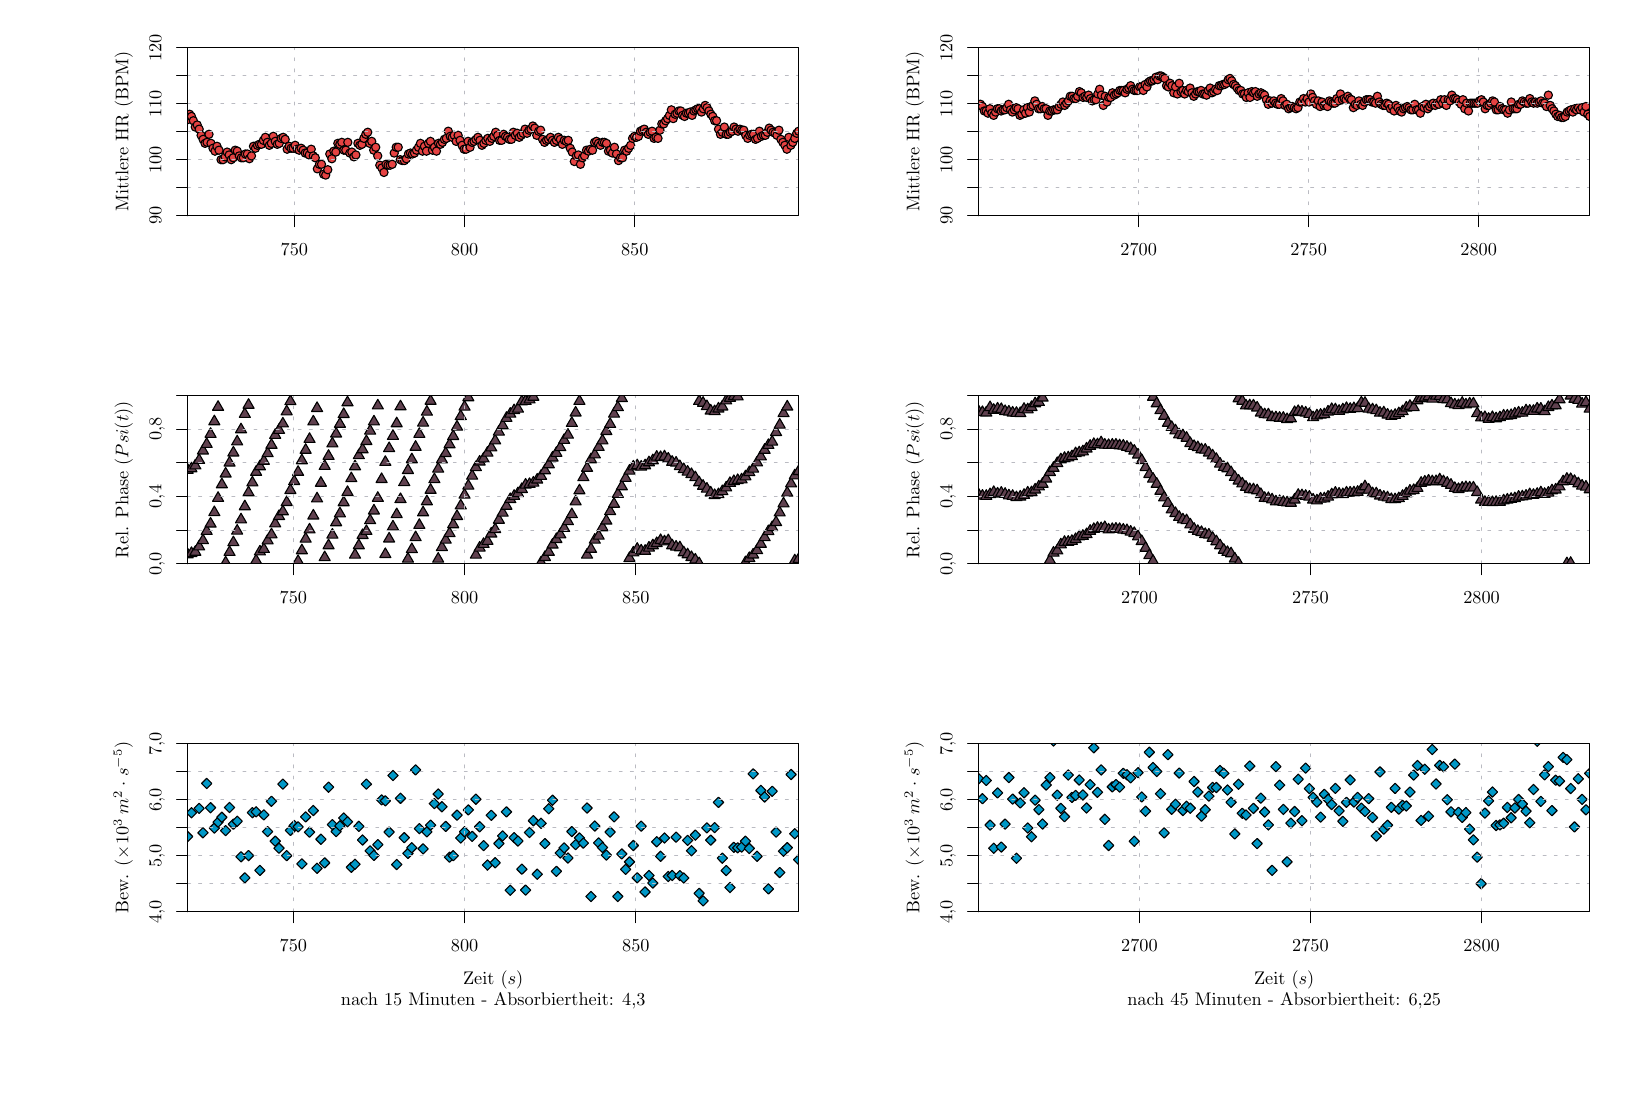
\begin{tikzpicture}[x=1pt,y=1pt]
\definecolor{fillColor}{RGB}{255,255,255}
\path[use as bounding box,fill=fillColor,fill opacity=0.00] (0,0) rectangle (571.66,377.25);
\begin{scope}
\path[clip] ( 57.82,309.32) rectangle (278.60,370.02);
\definecolor{drawColor}{RGB}{0,0,0}
\definecolor{fillColor}{RGB}{229,66,66}

\path[draw=drawColor,line width= 0.4pt,line join=round,line cap=round,fill=fillColor] ( 57.82,344.01) circle (  1.49);

\path[draw=drawColor,line width= 0.4pt,line join=round,line cap=round,fill=fillColor] ( 58.50,345.96) circle (  1.49);

\path[draw=drawColor,line width= 0.4pt,line join=round,line cap=round,fill=fillColor] ( 59.18,345.17) circle (  1.49);

\path[draw=drawColor,line width= 0.4pt,line join=round,line cap=round,fill=fillColor] ( 59.87,343.62) circle (  1.49);

\path[draw=drawColor,line width= 0.4pt,line join=round,line cap=round,fill=fillColor] ( 60.57,341.33) circle (  1.49);

\path[draw=drawColor,line width= 0.4pt,line join=round,line cap=round,fill=fillColor] ( 61.27,342.09) circle (  1.49);

\path[draw=drawColor,line width= 0.4pt,line join=round,line cap=round,fill=fillColor] ( 61.97,340.58) circle (  1.49);

\path[draw=drawColor,line width= 0.4pt,line join=round,line cap=round,fill=fillColor] ( 62.67,338.35) circle (  1.49);

\path[draw=drawColor,line width= 0.4pt,line join=round,line cap=round,fill=fillColor] ( 63.39,336.89) circle (  1.49);

\path[draw=drawColor,line width= 0.4pt,line join=round,line cap=round,fill=fillColor] ( 64.10,335.45) circle (  1.49);

\path[draw=drawColor,line width= 0.4pt,line join=round,line cap=round,fill=fillColor] ( 64.82,335.81) circle (  1.49);

\path[draw=drawColor,line width= 0.4pt,line join=round,line cap=round,fill=fillColor] ( 65.52,338.72) circle (  1.49);

\path[draw=drawColor,line width= 0.4pt,line join=round,line cap=round,fill=fillColor] ( 66.24,335.45) circle (  1.49);

\path[draw=drawColor,line width= 0.4pt,line join=round,line cap=round,fill=fillColor] ( 66.96,333.68) circle (  1.49);

\path[draw=drawColor,line width= 0.4pt,line join=round,line cap=round,fill=fillColor] ( 67.69,332.63) circle (  1.49);

\path[draw=drawColor,line width= 0.4pt,line join=round,line cap=round,fill=fillColor] ( 68.41,334.39) circle (  1.49);

\path[draw=drawColor,line width= 0.4pt,line join=round,line cap=round,fill=fillColor] ( 69.14,332.98) circle (  1.49);

\path[draw=drawColor,line width= 0.4pt,line join=round,line cap=round,fill=fillColor] ( 69.88,329.55) circle (  1.49);

\path[draw=drawColor,line width= 0.4pt,line join=round,line cap=round,fill=fillColor] ( 70.61,329.55) circle (  1.49);

\path[draw=drawColor,line width= 0.4pt,line join=round,line cap=round,fill=fillColor] ( 71.35,330.57) circle (  1.49);

\path[draw=drawColor,line width= 0.4pt,line join=round,line cap=round,fill=fillColor] ( 72.08,332.29) circle (  1.49);

\path[draw=drawColor,line width= 0.4pt,line join=round,line cap=round,fill=fillColor] ( 72.81,331.25) circle (  1.49);

\path[draw=drawColor,line width= 0.4pt,line join=round,line cap=round,fill=fillColor] ( 73.55,329.55) circle (  1.49);

\path[draw=drawColor,line width= 0.4pt,line join=round,line cap=round,fill=fillColor] ( 74.28,330.23) circle (  1.49);

\path[draw=drawColor,line width= 0.4pt,line join=round,line cap=round,fill=fillColor] ( 75.01,332.98) circle (  1.49);

\path[draw=drawColor,line width= 0.4pt,line join=round,line cap=round,fill=fillColor] ( 75.74,332.63) circle (  1.49);

\path[draw=drawColor,line width= 0.4pt,line join=round,line cap=round,fill=fillColor] ( 76.47,330.91) circle (  1.49);

\path[draw=drawColor,line width= 0.4pt,line join=round,line cap=round,fill=fillColor] ( 77.20,330.23) circle (  1.49);

\path[draw=drawColor,line width= 0.4pt,line join=round,line cap=round,fill=fillColor] ( 77.94,330.23) circle (  1.49);

\path[draw=drawColor,line width= 0.4pt,line join=round,line cap=round,fill=fillColor] ( 78.67,331.60) circle (  1.49);

\path[draw=drawColor,line width= 0.4pt,line join=round,line cap=round,fill=fillColor] ( 79.40,331.60) circle (  1.49);

\path[draw=drawColor,line width= 0.4pt,line join=round,line cap=round,fill=fillColor] ( 80.14,329.89) circle (  1.49);

\path[draw=drawColor,line width= 0.4pt,line join=round,line cap=round,fill=fillColor] ( 80.87,330.91) circle (  1.49);

\path[draw=drawColor,line width= 0.4pt,line join=round,line cap=round,fill=fillColor] ( 81.59,334.39) circle (  1.49);

\path[draw=drawColor,line width= 0.4pt,line join=round,line cap=round,fill=fillColor] ( 82.31,333.68) circle (  1.49);

\path[draw=drawColor,line width= 0.4pt,line join=round,line cap=round,fill=fillColor] ( 83.03,334.74) circle (  1.49);

\path[draw=drawColor,line width= 0.4pt,line join=round,line cap=round,fill=fillColor] ( 83.75,335.10) circle (  1.49);

\path[draw=drawColor,line width= 0.4pt,line join=round,line cap=round,fill=fillColor] ( 84.47,335.10) circle (  1.49);

\path[draw=drawColor,line width= 0.4pt,line join=round,line cap=round,fill=fillColor] ( 85.18,336.53) circle (  1.49);

\path[draw=drawColor,line width= 0.4pt,line join=round,line cap=round,fill=fillColor] ( 85.89,337.62) circle (  1.49);

\path[draw=drawColor,line width= 0.4pt,line join=round,line cap=round,fill=fillColor] ( 86.61,335.81) circle (  1.49);

\path[draw=drawColor,line width= 0.4pt,line join=round,line cap=round,fill=fillColor] ( 87.33,334.74) circle (  1.49);

\path[draw=drawColor,line width= 0.4pt,line join=round,line cap=round,fill=fillColor] ( 88.05,335.45) circle (  1.49);

\path[draw=drawColor,line width= 0.4pt,line join=round,line cap=round,fill=fillColor] ( 88.75,337.98) circle (  1.49);

\path[draw=drawColor,line width= 0.4pt,line join=round,line cap=round,fill=fillColor] ( 89.47,336.17) circle (  1.49);

\path[draw=drawColor,line width= 0.4pt,line join=round,line cap=round,fill=fillColor] ( 90.19,335.10) circle (  1.49);

\path[draw=drawColor,line width= 0.4pt,line join=round,line cap=round,fill=fillColor] ( 90.90,335.45) circle (  1.49);

\path[draw=drawColor,line width= 0.4pt,line join=round,line cap=round,fill=fillColor] ( 91.62,337.25) circle (  1.49);

\path[draw=drawColor,line width= 0.4pt,line join=round,line cap=round,fill=fillColor] ( 92.33,337.62) circle (  1.49);

\path[draw=drawColor,line width= 0.4pt,line join=round,line cap=round,fill=fillColor] ( 93.04,336.89) circle (  1.49);

\path[draw=drawColor,line width= 0.4pt,line join=round,line cap=round,fill=fillColor] ( 93.76,333.33) circle (  1.49);

\path[draw=drawColor,line width= 0.4pt,line join=round,line cap=round,fill=fillColor] ( 94.48,334.39) circle (  1.49);

\path[draw=drawColor,line width= 0.4pt,line join=round,line cap=round,fill=fillColor] ( 95.21,333.68) circle (  1.49);

\path[draw=drawColor,line width= 0.4pt,line join=round,line cap=round,fill=fillColor] ( 95.93,333.68) circle (  1.49);

\path[draw=drawColor,line width= 0.4pt,line join=round,line cap=round,fill=fillColor] ( 96.65,334.74) circle (  1.49);

\path[draw=drawColor,line width= 0.4pt,line join=round,line cap=round,fill=fillColor] ( 97.37,333.33) circle (  1.49);

\path[draw=drawColor,line width= 0.4pt,line join=round,line cap=round,fill=fillColor] ( 98.10,332.98) circle (  1.49);

\path[draw=drawColor,line width= 0.4pt,line join=round,line cap=round,fill=fillColor] ( 98.82,333.68) circle (  1.49);

\path[draw=drawColor,line width= 0.4pt,line join=round,line cap=round,fill=fillColor] ( 99.55,332.98) circle (  1.49);

\path[draw=drawColor,line width= 0.4pt,line join=round,line cap=round,fill=fillColor] (100.28,331.94) circle (  1.49);

\path[draw=drawColor,line width= 0.4pt,line join=round,line cap=round,fill=fillColor] (101.01,331.94) circle (  1.49);

\path[draw=drawColor,line width= 0.4pt,line join=round,line cap=round,fill=fillColor] (101.74,331.25) circle (  1.49);

\path[draw=drawColor,line width= 0.4pt,line join=round,line cap=round,fill=fillColor] (102.46,333.33) circle (  1.49);

\path[draw=drawColor,line width= 0.4pt,line join=round,line cap=round,fill=fillColor] (103.20,330.91) circle (  1.49);

\path[draw=drawColor,line width= 0.4pt,line join=round,line cap=round,fill=fillColor] (103.93,330.23) circle (  1.49);

\path[draw=drawColor,line width= 0.4pt,line join=round,line cap=round,fill=fillColor] (104.68,326.23) circle (  1.49);

\path[draw=drawColor,line width= 0.4pt,line join=round,line cap=round,fill=fillColor] (105.43,327.88) circle (  1.49);

\path[draw=drawColor,line width= 0.4pt,line join=round,line cap=round,fill=fillColor] (106.17,327.88) circle (  1.49);

\path[draw=drawColor,line width= 0.4pt,line join=round,line cap=round,fill=fillColor] (106.93,324.30) circle (  1.49);

\path[draw=drawColor,line width= 0.4pt,line join=round,line cap=round,fill=fillColor] (107.69,323.98) circle (  1.49);

\path[draw=drawColor,line width= 0.4pt,line join=round,line cap=round,fill=fillColor] (108.44,325.91) circle (  1.49);

\path[draw=drawColor,line width= 0.4pt,line join=round,line cap=round,fill=fillColor] (109.17,331.60) circle (  1.49);

\path[draw=drawColor,line width= 0.4pt,line join=round,line cap=round,fill=fillColor] (109.91,329.89) circle (  1.49);

\path[draw=drawColor,line width= 0.4pt,line join=round,line cap=round,fill=fillColor] (110.63,332.63) circle (  1.49);

\path[draw=drawColor,line width= 0.4pt,line join=round,line cap=round,fill=fillColor] (111.36,332.29) circle (  1.49);

\path[draw=drawColor,line width= 0.4pt,line join=round,line cap=round,fill=fillColor] (112.08,335.45) circle (  1.49);

\path[draw=drawColor,line width= 0.4pt,line join=round,line cap=round,fill=fillColor] (112.80,335.10) circle (  1.49);

\path[draw=drawColor,line width= 0.4pt,line join=round,line cap=round,fill=fillColor] (113.51,335.81) circle (  1.49);

\path[draw=drawColor,line width= 0.4pt,line join=round,line cap=round,fill=fillColor] (114.24,332.98) circle (  1.49);

\path[draw=drawColor,line width= 0.4pt,line join=round,line cap=round,fill=fillColor] (114.96,332.98) circle (  1.49);

\path[draw=drawColor,line width= 0.4pt,line join=round,line cap=round,fill=fillColor] (115.68,335.81) circle (  1.49);

\path[draw=drawColor,line width= 0.4pt,line join=round,line cap=round,fill=fillColor] (116.41,331.94) circle (  1.49);

\path[draw=drawColor,line width= 0.4pt,line join=round,line cap=round,fill=fillColor] (117.14,332.29) circle (  1.49);

\path[draw=drawColor,line width= 0.4pt,line join=round,line cap=round,fill=fillColor] (117.87,330.57) circle (  1.49);

\path[draw=drawColor,line width= 0.4pt,line join=round,line cap=round,fill=fillColor] (118.60,331.25) circle (  1.49);

\path[draw=drawColor,line width= 0.4pt,line join=round,line cap=round,fill=fillColor] (119.32,335.45) circle (  1.49);

\path[draw=drawColor,line width= 0.4pt,line join=round,line cap=round,fill=fillColor] (120.04,334.74) circle (  1.49);

\path[draw=drawColor,line width= 0.4pt,line join=round,line cap=round,fill=fillColor] (120.76,335.10) circle (  1.49);

\path[draw=drawColor,line width= 0.4pt,line join=round,line cap=round,fill=fillColor] (121.47,337.25) circle (  1.49);

\path[draw=drawColor,line width= 0.4pt,line join=round,line cap=round,fill=fillColor] (122.18,338.72) circle (  1.49);

\path[draw=drawColor,line width= 0.4pt,line join=round,line cap=round,fill=fillColor] (122.88,339.46) circle (  1.49);

\path[draw=drawColor,line width= 0.4pt,line join=round,line cap=round,fill=fillColor] (123.60,335.45) circle (  1.49);

\path[draw=drawColor,line width= 0.4pt,line join=round,line cap=round,fill=fillColor] (124.31,336.17) circle (  1.49);

\path[draw=drawColor,line width= 0.4pt,line join=round,line cap=round,fill=fillColor] (125.04,332.98) circle (  1.49);

\path[draw=drawColor,line width= 0.4pt,line join=round,line cap=round,fill=fillColor] (125.76,334.03) circle (  1.49);

\path[draw=drawColor,line width= 0.4pt,line join=round,line cap=round,fill=fillColor] (126.49,330.91) circle (  1.49);

\path[draw=drawColor,line width= 0.4pt,line join=round,line cap=round,fill=fillColor] (127.24,327.55) circle (  1.49);

\path[draw=drawColor,line width= 0.4pt,line join=round,line cap=round,fill=fillColor] (127.99,326.56) circle (  1.49);

\path[draw=drawColor,line width= 0.4pt,line join=round,line cap=round,fill=fillColor] (128.74,324.94) circle (  1.49);

\path[draw=drawColor,line width= 0.4pt,line join=round,line cap=round,fill=fillColor] (129.49,327.88) circle (  1.49);

\path[draw=drawColor,line width= 0.4pt,line join=round,line cap=round,fill=fillColor] (130.23,327.55) circle (  1.49);

\path[draw=drawColor,line width= 0.4pt,line join=round,line cap=round,fill=fillColor] (130.98,327.55) circle (  1.49);

\path[draw=drawColor,line width= 0.4pt,line join=round,line cap=round,fill=fillColor] (131.72,327.88) circle (  1.49);

\path[draw=drawColor,line width= 0.4pt,line join=round,line cap=round,fill=fillColor] (132.45,331.94) circle (  1.49);

\path[draw=drawColor,line width= 0.4pt,line join=round,line cap=round,fill=fillColor] (133.17,334.03) circle (  1.49);

\path[draw=drawColor,line width= 0.4pt,line join=round,line cap=round,fill=fillColor] (133.89,334.03) circle (  1.49);

\path[draw=drawColor,line width= 0.4pt,line join=round,line cap=round,fill=fillColor] (134.63,329.55) circle (  1.49);

\path[draw=drawColor,line width= 0.4pt,line join=round,line cap=round,fill=fillColor] (135.37,329.21) circle (  1.49);

\path[draw=drawColor,line width= 0.4pt,line join=round,line cap=round,fill=fillColor] (136.11,329.21) circle (  1.49);

\path[draw=drawColor,line width= 0.4pt,line join=round,line cap=round,fill=fillColor] (136.85,329.89) circle (  1.49);

\path[draw=drawColor,line width= 0.4pt,line join=round,line cap=round,fill=fillColor] (137.58,331.60) circle (  1.49);

\path[draw=drawColor,line width= 0.4pt,line join=round,line cap=round,fill=fillColor] (138.31,331.94) circle (  1.49);

\path[draw=drawColor,line width= 0.4pt,line join=round,line cap=round,fill=fillColor] (139.04,331.60) circle (  1.49);

\path[draw=drawColor,line width= 0.4pt,line join=round,line cap=round,fill=fillColor] (139.77,331.94) circle (  1.49);

\path[draw=drawColor,line width= 0.4pt,line join=round,line cap=round,fill=fillColor] (140.49,332.98) circle (  1.49);

\path[draw=drawColor,line width= 0.4pt,line join=round,line cap=round,fill=fillColor] (141.22,334.03) circle (  1.49);

\path[draw=drawColor,line width= 0.4pt,line join=round,line cap=round,fill=fillColor] (141.93,335.45) circle (  1.49);

\path[draw=drawColor,line width= 0.4pt,line join=round,line cap=round,fill=fillColor] (142.66,332.63) circle (  1.49);

\path[draw=drawColor,line width= 0.4pt,line join=round,line cap=round,fill=fillColor] (143.38,334.39) circle (  1.49);

\path[draw=drawColor,line width= 0.4pt,line join=round,line cap=round,fill=fillColor] (144.11,332.63) circle (  1.49);

\path[draw=drawColor,line width= 0.4pt,line join=round,line cap=round,fill=fillColor] (144.82,335.45) circle (  1.49);

\path[draw=drawColor,line width= 0.4pt,line join=round,line cap=round,fill=fillColor] (145.54,336.17) circle (  1.49);

\path[draw=drawColor,line width= 0.4pt,line join=round,line cap=round,fill=fillColor] (146.26,332.98) circle (  1.49);

\path[draw=drawColor,line width= 0.4pt,line join=round,line cap=round,fill=fillColor] (146.99,334.03) circle (  1.49);

\path[draw=drawColor,line width= 0.4pt,line join=round,line cap=round,fill=fillColor] (147.71,332.63) circle (  1.49);

\path[draw=drawColor,line width= 0.4pt,line join=round,line cap=round,fill=fillColor] (148.43,335.45) circle (  1.49);

\path[draw=drawColor,line width= 0.4pt,line join=round,line cap=round,fill=fillColor] (149.15,335.10) circle (  1.49);

\path[draw=drawColor,line width= 0.4pt,line join=round,line cap=round,fill=fillColor] (149.87,335.81) circle (  1.49);

\path[draw=drawColor,line width= 0.4pt,line join=round,line cap=round,fill=fillColor] (150.58,336.89) circle (  1.49);

\path[draw=drawColor,line width= 0.4pt,line join=round,line cap=round,fill=fillColor] (151.29,337.25) circle (  1.49);

\path[draw=drawColor,line width= 0.4pt,line join=round,line cap=round,fill=fillColor] (151.99,339.83) circle (  1.49);

\path[draw=drawColor,line width= 0.4pt,line join=round,line cap=round,fill=fillColor] (152.70,337.98) circle (  1.49);

\path[draw=drawColor,line width= 0.4pt,line join=round,line cap=round,fill=fillColor] (153.41,337.62) circle (  1.49);

\path[draw=drawColor,line width= 0.4pt,line join=round,line cap=round,fill=fillColor] (154.12,338.35) circle (  1.49);

\path[draw=drawColor,line width= 0.4pt,line join=round,line cap=round,fill=fillColor] (154.83,336.17) circle (  1.49);

\path[draw=drawColor,line width= 0.4pt,line join=round,line cap=round,fill=fillColor] (155.54,338.35) circle (  1.49);

\path[draw=drawColor,line width= 0.4pt,line join=round,line cap=round,fill=fillColor] (156.25,336.53) circle (  1.49);

\path[draw=drawColor,line width= 0.4pt,line join=round,line cap=round,fill=fillColor] (156.97,334.74) circle (  1.49);

\path[draw=drawColor,line width= 0.4pt,line join=round,line cap=round,fill=fillColor] (157.70,333.33) circle (  1.49);

\path[draw=drawColor,line width= 0.4pt,line join=round,line cap=round,fill=fillColor] (158.42,333.33) circle (  1.49);

\path[draw=drawColor,line width= 0.4pt,line join=round,line cap=round,fill=fillColor] (159.13,336.17) circle (  1.49);

\path[draw=drawColor,line width= 0.4pt,line join=round,line cap=round,fill=fillColor] (159.86,334.03) circle (  1.49);

\path[draw=drawColor,line width= 0.4pt,line join=round,line cap=round,fill=fillColor] (160.57,335.81) circle (  1.49);

\path[draw=drawColor,line width= 0.4pt,line join=round,line cap=round,fill=fillColor] (161.29,336.17) circle (  1.49);

\path[draw=drawColor,line width= 0.4pt,line join=round,line cap=round,fill=fillColor] (162.00,336.89) circle (  1.49);

\path[draw=drawColor,line width= 0.4pt,line join=round,line cap=round,fill=fillColor] (162.71,337.62) circle (  1.49);

\path[draw=drawColor,line width= 0.4pt,line join=round,line cap=round,fill=fillColor] (163.42,336.53) circle (  1.49);

\path[draw=drawColor,line width= 0.4pt,line join=round,line cap=round,fill=fillColor] (164.14,334.74) circle (  1.49);

\path[draw=drawColor,line width= 0.4pt,line join=round,line cap=round,fill=fillColor] (164.86,335.45) circle (  1.49);

\path[draw=drawColor,line width= 0.4pt,line join=round,line cap=round,fill=fillColor] (165.57,336.53) circle (  1.49);

\path[draw=drawColor,line width= 0.4pt,line join=round,line cap=round,fill=fillColor] (166.28,337.25) circle (  1.49);

\path[draw=drawColor,line width= 0.4pt,line join=round,line cap=round,fill=fillColor] (167.00,336.17) circle (  1.49);

\path[draw=drawColor,line width= 0.4pt,line join=round,line cap=round,fill=fillColor] (167.71,337.25) circle (  1.49);

\path[draw=drawColor,line width= 0.4pt,line join=round,line cap=round,fill=fillColor] (168.42,337.98) circle (  1.49);

\path[draw=drawColor,line width= 0.4pt,line join=round,line cap=round,fill=fillColor] (169.12,339.46) circle (  1.49);

\path[draw=drawColor,line width= 0.4pt,line join=round,line cap=round,fill=fillColor] (169.83,338.35) circle (  1.49);

\path[draw=drawColor,line width= 0.4pt,line join=round,line cap=round,fill=fillColor] (170.54,336.53) circle (  1.49);

\path[draw=drawColor,line width= 0.4pt,line join=round,line cap=round,fill=fillColor] (171.26,336.53) circle (  1.49);

\path[draw=drawColor,line width= 0.4pt,line join=round,line cap=round,fill=fillColor] (171.96,338.72) circle (  1.49);

\path[draw=drawColor,line width= 0.4pt,line join=round,line cap=round,fill=fillColor] (172.67,337.98) circle (  1.49);

\path[draw=drawColor,line width= 0.4pt,line join=round,line cap=round,fill=fillColor] (173.38,337.62) circle (  1.49);

\path[draw=drawColor,line width= 0.4pt,line join=round,line cap=round,fill=fillColor] (174.09,336.89) circle (  1.49);

\path[draw=drawColor,line width= 0.4pt,line join=round,line cap=round,fill=fillColor] (174.80,336.89) circle (  1.49);

\path[draw=drawColor,line width= 0.4pt,line join=round,line cap=round,fill=fillColor] (175.51,339.46) circle (  1.49);

\path[draw=drawColor,line width= 0.4pt,line join=round,line cap=round,fill=fillColor] (176.21,338.35) circle (  1.49);

\path[draw=drawColor,line width= 0.4pt,line join=round,line cap=round,fill=fillColor] (176.92,339.09) circle (  1.49);

\path[draw=drawColor,line width= 0.4pt,line join=round,line cap=round,fill=fillColor] (177.63,337.62) circle (  1.49);

\path[draw=drawColor,line width= 0.4pt,line join=round,line cap=round,fill=fillColor] (178.34,338.35) circle (  1.49);

\path[draw=drawColor,line width= 0.4pt,line join=round,line cap=round,fill=fillColor] (179.04,339.09) circle (  1.49);

\path[draw=drawColor,line width= 0.4pt,line join=round,line cap=round,fill=fillColor] (179.74,340.58) circle (  1.49);

\path[draw=drawColor,line width= 0.4pt,line join=round,line cap=round,fill=fillColor] (180.45,339.09) circle (  1.49);

\path[draw=drawColor,line width= 0.4pt,line join=round,line cap=round,fill=fillColor] (181.15,340.20) circle (  1.49);

\path[draw=drawColor,line width= 0.4pt,line join=round,line cap=round,fill=fillColor] (181.85,340.58) circle (  1.49);

\path[draw=drawColor,line width= 0.4pt,line join=round,line cap=round,fill=fillColor] (182.54,341.71) circle (  1.49);

\path[draw=drawColor,line width= 0.4pt,line join=round,line cap=round,fill=fillColor] (183.24,340.95) circle (  1.49);

\path[draw=drawColor,line width= 0.4pt,line join=round,line cap=round,fill=fillColor] (183.95,338.35) circle (  1.49);

\path[draw=drawColor,line width= 0.4pt,line join=round,line cap=round,fill=fillColor] (184.65,339.83) circle (  1.49);

\path[draw=drawColor,line width= 0.4pt,line join=round,line cap=round,fill=fillColor] (185.35,340.20) circle (  1.49);

\path[draw=drawColor,line width= 0.4pt,line join=round,line cap=round,fill=fillColor] (186.06,336.89) circle (  1.49);

\path[draw=drawColor,line width= 0.4pt,line join=round,line cap=round,fill=fillColor] (186.78,335.81) circle (  1.49);

\path[draw=drawColor,line width= 0.4pt,line join=round,line cap=round,fill=fillColor] (187.49,336.53) circle (  1.49);

\path[draw=drawColor,line width= 0.4pt,line join=round,line cap=round,fill=fillColor] (188.21,336.89) circle (  1.49);

\path[draw=drawColor,line width= 0.4pt,line join=round,line cap=round,fill=fillColor] (188.92,337.62) circle (  1.49);

\path[draw=drawColor,line width= 0.4pt,line join=round,line cap=round,fill=fillColor] (189.63,336.53) circle (  1.49);

\path[draw=drawColor,line width= 0.4pt,line join=round,line cap=round,fill=fillColor] (190.35,335.81) circle (  1.49);

\path[draw=drawColor,line width= 0.4pt,line join=round,line cap=round,fill=fillColor] (191.06,336.53) circle (  1.49);

\path[draw=drawColor,line width= 0.4pt,line join=round,line cap=round,fill=fillColor] (191.77,337.62) circle (  1.49);

\path[draw=drawColor,line width= 0.4pt,line join=round,line cap=round,fill=fillColor] (192.48,336.89) circle (  1.49);

\path[draw=drawColor,line width= 0.4pt,line join=round,line cap=round,fill=fillColor] (193.20,335.10) circle (  1.49);

\path[draw=drawColor,line width= 0.4pt,line join=round,line cap=round,fill=fillColor] (193.91,336.53) circle (  1.49);

\path[draw=drawColor,line width= 0.4pt,line join=round,line cap=round,fill=fillColor] (194.63,336.17) circle (  1.49);

\path[draw=drawColor,line width= 0.4pt,line join=round,line cap=round,fill=fillColor] (195.34,336.53) circle (  1.49);

\path[draw=drawColor,line width= 0.4pt,line join=round,line cap=round,fill=fillColor] (196.06,333.68) circle (  1.49);

\path[draw=drawColor,line width= 0.4pt,line join=round,line cap=round,fill=fillColor] (196.79,332.29) circle (  1.49);

\path[draw=drawColor,line width= 0.4pt,line join=round,line cap=round,fill=fillColor] (197.53,328.88) circle (  1.49);

\path[draw=drawColor,line width= 0.4pt,line join=round,line cap=round,fill=fillColor] (198.27,330.91) circle (  1.49);

\path[draw=drawColor,line width= 0.4pt,line join=round,line cap=round,fill=fillColor] (199.00,331.25) circle (  1.49);

\path[draw=drawColor,line width= 0.4pt,line join=round,line cap=round,fill=fillColor] (199.74,327.88) circle (  1.49);

\path[draw=drawColor,line width= 0.4pt,line join=round,line cap=round,fill=fillColor] (200.48,330.23) circle (  1.49);

\path[draw=drawColor,line width= 0.4pt,line join=round,line cap=round,fill=fillColor] (201.21,330.91) circle (  1.49);

\path[draw=drawColor,line width= 0.4pt,line join=round,line cap=round,fill=fillColor] (201.94,332.98) circle (  1.49);

\path[draw=drawColor,line width= 0.4pt,line join=round,line cap=round,fill=fillColor] (202.66,332.63) circle (  1.49);

\path[draw=drawColor,line width= 0.4pt,line join=round,line cap=round,fill=fillColor] (203.39,333.33) circle (  1.49);

\path[draw=drawColor,line width= 0.4pt,line join=round,line cap=round,fill=fillColor] (204.11,332.98) circle (  1.49);

\path[draw=drawColor,line width= 0.4pt,line join=round,line cap=round,fill=fillColor] (204.83,335.81) circle (  1.49);

\path[draw=drawColor,line width= 0.4pt,line join=round,line cap=round,fill=fillColor] (205.54,336.17) circle (  1.49);

\path[draw=drawColor,line width= 0.4pt,line join=round,line cap=round,fill=fillColor] (206.26,335.45) circle (  1.49);

\path[draw=drawColor,line width= 0.4pt,line join=round,line cap=round,fill=fillColor] (206.98,334.74) circle (  1.49);

\path[draw=drawColor,line width= 0.4pt,line join=round,line cap=round,fill=fillColor] (207.70,335.81) circle (  1.49);

\path[draw=drawColor,line width= 0.4pt,line join=round,line cap=round,fill=fillColor] (208.41,335.81) circle (  1.49);

\path[draw=drawColor,line width= 0.4pt,line join=round,line cap=round,fill=fillColor] (209.13,335.45) circle (  1.49);

\path[draw=drawColor,line width= 0.4pt,line join=round,line cap=round,fill=fillColor] (209.86,332.63) circle (  1.49);

\path[draw=drawColor,line width= 0.4pt,line join=round,line cap=round,fill=fillColor] (210.58,332.98) circle (  1.49);

\path[draw=drawColor,line width= 0.4pt,line join=round,line cap=round,fill=fillColor] (211.31,331.94) circle (  1.49);

\path[draw=drawColor,line width= 0.4pt,line join=round,line cap=round,fill=fillColor] (212.03,334.03) circle (  1.49);

\path[draw=drawColor,line width= 0.4pt,line join=round,line cap=round,fill=fillColor] (212.76,331.60) circle (  1.49);

\path[draw=drawColor,line width= 0.4pt,line join=round,line cap=round,fill=fillColor] (213.50,329.21) circle (  1.49);

\path[draw=drawColor,line width= 0.4pt,line join=round,line cap=round,fill=fillColor] (214.24,330.23) circle (  1.49);

\path[draw=drawColor,line width= 0.4pt,line join=round,line cap=round,fill=fillColor] (214.97,330.23) circle (  1.49);

\path[draw=drawColor,line width= 0.4pt,line join=round,line cap=round,fill=fillColor] (215.70,332.98) circle (  1.49);

\path[draw=drawColor,line width= 0.4pt,line join=round,line cap=round,fill=fillColor] (216.43,332.63) circle (  1.49);

\path[draw=drawColor,line width= 0.4pt,line join=round,line cap=round,fill=fillColor] (217.15,333.68) circle (  1.49);

\path[draw=drawColor,line width= 0.4pt,line join=round,line cap=round,fill=fillColor] (217.87,334.74) circle (  1.49);

\path[draw=drawColor,line width= 0.4pt,line join=round,line cap=round,fill=fillColor] (218.58,337.25) circle (  1.49);

\path[draw=drawColor,line width= 0.4pt,line join=round,line cap=round,fill=fillColor] (219.29,337.98) circle (  1.49);

\path[draw=drawColor,line width= 0.4pt,line join=round,line cap=round,fill=fillColor] (220.00,337.62) circle (  1.49);

\path[draw=drawColor,line width= 0.4pt,line join=round,line cap=round,fill=fillColor] (220.71,337.98) circle (  1.49);

\path[draw=drawColor,line width= 0.4pt,line join=round,line cap=round,fill=fillColor] (221.41,339.83) circle (  1.49);

\path[draw=drawColor,line width= 0.4pt,line join=round,line cap=round,fill=fillColor] (222.11,340.20) circle (  1.49);

\path[draw=drawColor,line width= 0.4pt,line join=round,line cap=round,fill=fillColor] (222.81,340.58) circle (  1.49);

\path[draw=drawColor,line width= 0.4pt,line join=round,line cap=round,fill=fillColor] (223.51,339.46) circle (  1.49);

\path[draw=drawColor,line width= 0.4pt,line join=round,line cap=round,fill=fillColor] (224.22,338.72) circle (  1.49);

\path[draw=drawColor,line width= 0.4pt,line join=round,line cap=round,fill=fillColor] (224.92,339.46) circle (  1.49);

\path[draw=drawColor,line width= 0.4pt,line join=round,line cap=round,fill=fillColor] (225.63,339.83) circle (  1.49);

\path[draw=drawColor,line width= 0.4pt,line join=round,line cap=round,fill=fillColor] (226.34,337.25) circle (  1.49);

\path[draw=drawColor,line width= 0.4pt,line join=round,line cap=round,fill=fillColor] (227.05,337.62) circle (  1.49);

\path[draw=drawColor,line width= 0.4pt,line join=round,line cap=round,fill=fillColor] (227.76,337.25) circle (  1.49);

\path[draw=drawColor,line width= 0.4pt,line join=round,line cap=round,fill=fillColor] (228.46,340.20) circle (  1.49);

\path[draw=drawColor,line width= 0.4pt,line join=round,line cap=round,fill=fillColor] (229.15,342.47) circle (  1.49);

\path[draw=drawColor,line width= 0.4pt,line join=round,line cap=round,fill=fillColor] (229.85,342.47) circle (  1.49);

\path[draw=drawColor,line width= 0.4pt,line join=round,line cap=round,fill=fillColor] (230.54,343.62) circle (  1.49);

\path[draw=drawColor,line width= 0.4pt,line join=round,line cap=round,fill=fillColor] (231.22,344.39) circle (  1.49);

\path[draw=drawColor,line width= 0.4pt,line join=round,line cap=round,fill=fillColor] (231.91,345.56) circle (  1.49);

\path[draw=drawColor,line width= 0.4pt,line join=round,line cap=round,fill=fillColor] (232.59,347.55) circle (  1.49);

\path[draw=drawColor,line width= 0.4pt,line join=round,line cap=round,fill=fillColor] (233.27,344.39) circle (  1.49);

\path[draw=drawColor,line width= 0.4pt,line join=round,line cap=round,fill=fillColor] (233.96,345.96) circle (  1.49);

\path[draw=drawColor,line width= 0.4pt,line join=round,line cap=round,fill=fillColor] (234.64,346.35) circle (  1.49);

\path[draw=drawColor,line width= 0.4pt,line join=round,line cap=round,fill=fillColor] (235.32,347.15) circle (  1.49);

\path[draw=drawColor,line width= 0.4pt,line join=round,line cap=round,fill=fillColor] (236.00,347.15) circle (  1.49);

\path[draw=drawColor,line width= 0.4pt,line join=round,line cap=round,fill=fillColor] (236.68,345.56) circle (  1.49);

\path[draw=drawColor,line width= 0.4pt,line join=round,line cap=round,fill=fillColor] (237.36,345.17) circle (  1.49);

\path[draw=drawColor,line width= 0.4pt,line join=round,line cap=round,fill=fillColor] (238.05,346.35) circle (  1.49);

\path[draw=drawColor,line width= 0.4pt,line join=round,line cap=round,fill=fillColor] (238.73,346.35) circle (  1.49);

\path[draw=drawColor,line width= 0.4pt,line join=round,line cap=round,fill=fillColor] (239.41,346.75) circle (  1.49);

\path[draw=drawColor,line width= 0.4pt,line join=round,line cap=round,fill=fillColor] (240.09,345.56) circle (  1.49);

\path[draw=drawColor,line width= 0.4pt,line join=round,line cap=round,fill=fillColor] (240.77,347.15) circle (  1.49);

\path[draw=drawColor,line width= 0.4pt,line join=round,line cap=round,fill=fillColor] (241.45,347.55) circle (  1.49);

\path[draw=drawColor,line width= 0.4pt,line join=round,line cap=round,fill=fillColor] (242.12,347.95) circle (  1.49);

\path[draw=drawColor,line width= 0.4pt,line join=round,line cap=round,fill=fillColor] (242.80,347.95) circle (  1.49);

\path[draw=drawColor,line width= 0.4pt,line join=round,line cap=round,fill=fillColor] (243.48,346.75) circle (  1.49);

\path[draw=drawColor,line width= 0.4pt,line join=round,line cap=round,fill=fillColor] (244.16,347.95) circle (  1.49);

\path[draw=drawColor,line width= 0.4pt,line join=round,line cap=round,fill=fillColor] (244.83,349.16) circle (  1.49);

\path[draw=drawColor,line width= 0.4pt,line join=round,line cap=round,fill=fillColor] (245.51,348.35) circle (  1.49);

\path[draw=drawColor,line width= 0.4pt,line join=round,line cap=round,fill=fillColor] (246.18,347.15) circle (  1.49);

\path[draw=drawColor,line width= 0.4pt,line join=round,line cap=round,fill=fillColor] (246.87,345.96) circle (  1.49);

\path[draw=drawColor,line width= 0.4pt,line join=round,line cap=round,fill=fillColor] (247.55,345.17) circle (  1.49);

\path[draw=drawColor,line width= 0.4pt,line join=round,line cap=round,fill=fillColor] (248.24,343.62) circle (  1.49);

\path[draw=drawColor,line width= 0.4pt,line join=round,line cap=round,fill=fillColor] (248.93,343.62) circle (  1.49);

\path[draw=drawColor,line width= 0.4pt,line join=round,line cap=round,fill=fillColor] (249.63,340.58) circle (  1.49);

\path[draw=drawColor,line width= 0.4pt,line join=round,line cap=round,fill=fillColor] (250.34,338.72) circle (  1.49);

\path[draw=drawColor,line width= 0.4pt,line join=round,line cap=round,fill=fillColor] (251.04,339.46) circle (  1.49);

\path[draw=drawColor,line width= 0.4pt,line join=round,line cap=round,fill=fillColor] (251.74,341.33) circle (  1.49);

\path[draw=drawColor,line width= 0.4pt,line join=round,line cap=round,fill=fillColor] (252.45,338.72) circle (  1.49);

\path[draw=drawColor,line width= 0.4pt,line join=round,line cap=round,fill=fillColor] (253.15,338.72) circle (  1.49);

\path[draw=drawColor,line width= 0.4pt,line join=round,line cap=round,fill=fillColor] (253.86,339.46) circle (  1.49);

\path[draw=drawColor,line width= 0.4pt,line join=round,line cap=round,fill=fillColor] (254.56,339.83) circle (  1.49);

\path[draw=drawColor,line width= 0.4pt,line join=round,line cap=round,fill=fillColor] (255.25,341.33) circle (  1.49);

\path[draw=drawColor,line width= 0.4pt,line join=round,line cap=round,fill=fillColor] (255.95,340.58) circle (  1.49);

\path[draw=drawColor,line width= 0.4pt,line join=round,line cap=round,fill=fillColor] (256.66,339.83) circle (  1.49);

\path[draw=drawColor,line width= 0.4pt,line join=round,line cap=round,fill=fillColor] (257.36,340.58) circle (  1.49);

\path[draw=drawColor,line width= 0.4pt,line join=round,line cap=round,fill=fillColor] (258.06,340.20) circle (  1.49);

\path[draw=drawColor,line width= 0.4pt,line join=round,line cap=round,fill=fillColor] (258.76,340.20) circle (  1.49);

\path[draw=drawColor,line width= 0.4pt,line join=round,line cap=round,fill=fillColor] (259.47,338.35) circle (  1.49);

\path[draw=drawColor,line width= 0.4pt,line join=round,line cap=round,fill=fillColor] (260.18,337.25) circle (  1.49);

\path[draw=drawColor,line width= 0.4pt,line join=round,line cap=round,fill=fillColor] (260.88,338.35) circle (  1.49);

\path[draw=drawColor,line width= 0.4pt,line join=round,line cap=round,fill=fillColor] (261.59,338.72) circle (  1.49);

\path[draw=drawColor,line width= 0.4pt,line join=round,line cap=round,fill=fillColor] (262.30,338.72) circle (  1.49);

\path[draw=drawColor,line width= 0.4pt,line join=round,line cap=round,fill=fillColor] (263.01,336.89) circle (  1.49);

\path[draw=drawColor,line width= 0.4pt,line join=round,line cap=round,fill=fillColor] (263.72,337.25) circle (  1.49);

\path[draw=drawColor,line width= 0.4pt,line join=round,line cap=round,fill=fillColor] (264.42,339.83) circle (  1.49);

\path[draw=drawColor,line width= 0.4pt,line join=round,line cap=round,fill=fillColor] (265.13,337.98) circle (  1.49);

\path[draw=drawColor,line width= 0.4pt,line join=round,line cap=round,fill=fillColor] (265.84,338.35) circle (  1.49);

\path[draw=drawColor,line width= 0.4pt,line join=round,line cap=round,fill=fillColor] (266.55,338.35) circle (  1.49);

\path[draw=drawColor,line width= 0.4pt,line join=round,line cap=round,fill=fillColor] (267.25,339.46) circle (  1.49);

\path[draw=drawColor,line width= 0.4pt,line join=round,line cap=round,fill=fillColor] (267.95,340.95) circle (  1.49);

\path[draw=drawColor,line width= 0.4pt,line join=round,line cap=round,fill=fillColor] (268.65,340.20) circle (  1.49);

\path[draw=drawColor,line width= 0.4pt,line join=round,line cap=round,fill=fillColor] (269.35,339.46) circle (  1.49);

\path[draw=drawColor,line width= 0.4pt,line join=round,line cap=round,fill=fillColor] (270.06,339.09) circle (  1.49);

\path[draw=drawColor,line width= 0.4pt,line join=round,line cap=round,fill=fillColor] (270.76,338.35) circle (  1.49);

\path[draw=drawColor,line width= 0.4pt,line join=round,line cap=round,fill=fillColor] (271.47,340.20) circle (  1.49);

\path[draw=drawColor,line width= 0.4pt,line join=round,line cap=round,fill=fillColor] (272.18,336.89) circle (  1.49);

\path[draw=drawColor,line width= 0.4pt,line join=round,line cap=round,fill=fillColor] (272.89,335.81) circle (  1.49);

\path[draw=drawColor,line width= 0.4pt,line join=round,line cap=round,fill=fillColor] (273.61,334.74) circle (  1.49);

\path[draw=drawColor,line width= 0.4pt,line join=round,line cap=round,fill=fillColor] (274.34,333.33) circle (  1.49);

\path[draw=drawColor,line width= 0.4pt,line join=round,line cap=round,fill=fillColor] (275.05,337.62) circle (  1.49);

\path[draw=drawColor,line width= 0.4pt,line join=round,line cap=round,fill=fillColor] (275.77,334.74) circle (  1.49);

\path[draw=drawColor,line width= 0.4pt,line join=round,line cap=round,fill=fillColor] (276.48,335.81) circle (  1.49);

\path[draw=drawColor,line width= 0.4pt,line join=round,line cap=round,fill=fillColor] (277.19,337.25) circle (  1.49);

\path[draw=drawColor,line width= 0.4pt,line join=round,line cap=round,fill=fillColor] (277.90,339.09) circle (  1.49);

\path[draw=drawColor,line width= 0.4pt,line join=round,line cap=round,fill=fillColor] (278.60,339.83) circle (  1.49);
\end{scope}
\begin{scope}
\path[clip] (  0.00,  0.00) rectangle (571.66,377.25);
\definecolor{drawColor}{RGB}{0,0,0}

\path[draw=drawColor,line width= 0.4pt,line join=round,line cap=round] ( 96.39,309.32) -- (219.39,309.32);

\path[draw=drawColor,line width= 0.4pt,line join=round,line cap=round] ( 96.39,309.32) -- ( 96.39,305.36);

\path[draw=drawColor,line width= 0.4pt,line join=round,line cap=round] (157.89,309.32) -- (157.89,305.36);

\path[draw=drawColor,line width= 0.4pt,line join=round,line cap=round] (219.39,309.32) -- (219.39,305.36);

\node[text=drawColor,anchor=base,inner sep=0pt, outer sep=0pt, scale=  0.66] at ( 96.39,295.06) {750};

\node[text=drawColor,anchor=base,inner sep=0pt, outer sep=0pt, scale=  0.66] at (157.89,295.06) {800};

\node[text=drawColor,anchor=base,inner sep=0pt, outer sep=0pt, scale=  0.66] at (219.39,295.06) {850};

\path[draw=drawColor,line width= 0.4pt,line join=round,line cap=round] ( 57.82,309.32) -- ( 57.82,370.02);

\path[draw=drawColor,line width= 0.4pt,line join=round,line cap=round] ( 57.82,309.32) -- ( 53.86,309.32);

\path[draw=drawColor,line width= 0.4pt,line join=round,line cap=round] ( 57.82,319.43) -- ( 53.86,319.43);

\path[draw=drawColor,line width= 0.4pt,line join=round,line cap=round] ( 57.82,329.55) -- ( 53.86,329.55);

\path[draw=drawColor,line width= 0.4pt,line join=round,line cap=round] ( 57.82,339.67) -- ( 53.86,339.67);

\path[draw=drawColor,line width= 0.4pt,line join=round,line cap=round] ( 57.82,349.79) -- ( 53.86,349.79);

\path[draw=drawColor,line width= 0.4pt,line join=round,line cap=round] ( 57.82,359.90) -- ( 53.86,359.90);

\path[draw=drawColor,line width= 0.4pt,line join=round,line cap=round] ( 57.82,370.02) -- ( 53.86,370.02);

\node[text=drawColor,rotate= 90.00,anchor=base,inner sep=0pt, outer sep=0pt, scale=  0.66] at ( 48.31,309.32) {90};

\node[text=drawColor,rotate= 90.00,anchor=base,inner sep=0pt, outer sep=0pt, scale=  0.66] at ( 48.31,329.55) {100};

\node[text=drawColor,rotate= 90.00,anchor=base,inner sep=0pt, outer sep=0pt, scale=  0.66] at ( 48.31,349.79) {110};

\node[text=drawColor,rotate= 90.00,anchor=base,inner sep=0pt, outer sep=0pt, scale=  0.66] at ( 48.31,370.02) {120};

\path[draw=drawColor,line width= 0.4pt,line join=round,line cap=round] ( 57.82,309.32) --
	(278.60,309.32) --
	(278.60,370.02) --
	( 57.82,370.02) --
	( 57.82,309.32);
\end{scope}
\begin{scope}
\path[clip] (  0.00,251.50) rectangle (285.83,377.25);
\definecolor{drawColor}{RGB}{0,0,0}

\node[text=drawColor,rotate= 90.00,anchor=base,inner sep=0pt, outer sep=0pt, scale=  0.66] at ( 36.43,339.67) {Mittlere HR (BPM)};
\end{scope}
\begin{scope}
\path[clip] ( 57.82,309.32) rectangle (278.60,370.02);
\definecolor{drawColor}{RGB}{186,187,194}

\path[draw=drawColor,line width= 0.4pt,dash pattern=on 1pt off 3pt ,line join=round,line cap=round] ( 96.39,309.32) -- ( 96.39,370.02);

\path[draw=drawColor,line width= 0.4pt,dash pattern=on 1pt off 3pt ,line join=round,line cap=round] (157.89,309.32) -- (157.89,370.02);

\path[draw=drawColor,line width= 0.4pt,dash pattern=on 1pt off 3pt ,line join=round,line cap=round] (219.39,309.32) -- (219.39,370.02);

\path[draw=drawColor,line width= 0.4pt,dash pattern=on 1pt off 3pt ,line join=round,line cap=round] ( 57.82,309.32) -- (278.60,309.32);

\path[draw=drawColor,line width= 0.4pt,dash pattern=on 1pt off 3pt ,line join=round,line cap=round] ( 57.82,319.43) -- (278.60,319.43);

\path[draw=drawColor,line width= 0.4pt,dash pattern=on 1pt off 3pt ,line join=round,line cap=round] ( 57.82,329.55) -- (278.60,329.55);

\path[draw=drawColor,line width= 0.4pt,dash pattern=on 1pt off 3pt ,line join=round,line cap=round] ( 57.82,339.67) -- (278.60,339.67);

\path[draw=drawColor,line width= 0.4pt,dash pattern=on 1pt off 3pt ,line join=round,line cap=round] ( 57.82,349.79) -- (278.60,349.79);

\path[draw=drawColor,line width= 0.4pt,dash pattern=on 1pt off 3pt ,line join=round,line cap=round] ( 57.82,359.90) -- (278.60,359.90);

\path[draw=drawColor,line width= 0.4pt,dash pattern=on 1pt off 3pt ,line join=round,line cap=round] ( 57.82,370.02) -- (278.60,370.02);
\end{scope}
\begin{scope}
\path[clip] (  0.00,  0.00) rectangle (571.66,377.25);
\definecolor{drawColor}{RGB}{0,0,0}

\path[draw=drawColor,line width= 0.4pt,line join=round,line cap=round] ( 57.82,309.32) --
	(278.60,309.32) --
	(278.60,370.02) --
	( 57.82,370.02) --
	( 57.82,309.32);
\end{scope}
\begin{scope}
\path[clip] ( 57.82,183.57) rectangle (278.60,244.27);
\definecolor{drawColor}{RGB}{0,0,0}
\definecolor{fillColor}{RGB}{96,65,79}

\path[draw=drawColor,line width= 0.4pt,line join=round,line cap=round,fill=fillColor] ( 57.82,189.15) --
	( 59.82,185.69) --
	( 55.82,185.69) --
	cycle;

\path[draw=drawColor,line width= 0.4pt,line join=round,line cap=round,fill=fillColor] ( 57.82,219.69) --
	( 59.82,216.22) --
	( 55.82,216.22) --
	cycle;

\path[draw=drawColor,line width= 0.4pt,line join=round,line cap=round,fill=fillColor] ( 59.19,189.64) --
	( 61.19,186.17) --
	( 57.19,186.17) --
	cycle;

\path[draw=drawColor,line width= 0.4pt,line join=round,line cap=round,fill=fillColor] ( 59.19,220.24) --
	( 61.19,216.77) --
	( 57.19,216.77) --
	cycle;

\path[draw=drawColor,line width= 0.4pt,line join=round,line cap=round,fill=fillColor] ( 60.58,190.06) --
	( 62.58,186.60) --
	( 58.58,186.60) --
	cycle;

\path[draw=drawColor,line width= 0.4pt,line join=round,line cap=round,fill=fillColor] ( 60.58,221.27) --
	( 62.58,217.80) --
	( 58.58,217.80) --
	cycle;

\path[draw=drawColor,line width= 0.4pt,line join=round,line cap=round,fill=fillColor] ( 61.95,192.01) --
	( 63.95,188.54) --
	( 59.95,188.54) --
	cycle;

\path[draw=drawColor,line width= 0.4pt,line join=round,line cap=round,fill=fillColor] ( 61.95,223.27) --
	( 63.95,219.81) --
	( 59.95,219.81) --
	cycle;

\path[draw=drawColor,line width= 0.4pt,line join=round,line cap=round,fill=fillColor] ( 63.34,194.25) --
	( 65.34,190.79) --
	( 61.34,190.79) --
	cycle;

\path[draw=drawColor,line width= 0.4pt,line join=round,line cap=round,fill=fillColor] ( 63.34,226.67) --
	( 65.34,223.21) --
	( 61.34,223.21) --
	cycle;

\path[draw=drawColor,line width= 0.4pt,line join=round,line cap=round,fill=fillColor] ( 64.69,197.59) --
	( 66.69,194.13) --
	( 62.69,194.13) --
	cycle;

\path[draw=drawColor,line width= 0.4pt,line join=round,line cap=round,fill=fillColor] ( 64.69,229.04) --
	( 66.69,225.57) --
	( 62.69,225.57) --
	cycle;

\path[draw=drawColor,line width= 0.4pt,line join=round,line cap=round,fill=fillColor] ( 66.08,200.26) --
	( 68.08,196.80) --
	( 64.08,196.80) --
	cycle;

\path[draw=drawColor,line width= 0.4pt,line join=round,line cap=round,fill=fillColor] ( 66.08,232.68) --
	( 68.08,229.22) --
	( 64.08,229.22) --
	cycle;

\path[draw=drawColor,line width= 0.4pt,line join=round,line cap=round,fill=fillColor] ( 67.45,204.39) --
	( 69.45,200.93) --
	( 65.45,200.93) --
	cycle;

\path[draw=drawColor,line width= 0.4pt,line join=round,line cap=round,fill=fillColor] ( 67.45,237.23) --
	( 69.45,233.77) --
	( 65.45,233.77) --
	cycle;

\path[draw=drawColor,line width= 0.4pt,line join=round,line cap=round,fill=fillColor] ( 68.80,209.55) --
	( 70.80,206.09) --
	( 66.80,206.09) --
	cycle;

\path[draw=drawColor,line width= 0.4pt,line join=round,line cap=round,fill=fillColor] ( 68.80,242.45) --
	( 70.80,238.99) --
	( 66.80,238.99) --
	cycle;

\path[draw=drawColor,line width= 0.4pt,line join=round,line cap=round,fill=fillColor] ( 70.17,214.47) --
	( 72.17,211.00) --
	( 68.17,211.00) --
	cycle;

\path[draw=drawColor,line width= 0.4pt,line join=round,line cap=round,fill=fillColor] ( 71.54,186.24) --
	( 73.54,182.78) --
	( 69.54,182.78) --
	cycle;

\path[draw=drawColor,line width= 0.4pt,line join=round,line cap=round,fill=fillColor] ( 71.54,218.35) --
	( 73.54,214.89) --
	( 69.54,214.89) --
	cycle;

\path[draw=drawColor,line width= 0.4pt,line join=round,line cap=round,fill=fillColor] ( 72.94,190.00) --
	( 74.94,186.54) --
	( 70.94,186.54) --
	cycle;

\path[draw=drawColor,line width= 0.4pt,line join=round,line cap=round,fill=fillColor] ( 72.94,222.30) --
	( 74.94,218.84) --
	( 70.94,218.84) --
	cycle;

\path[draw=drawColor,line width= 0.4pt,line join=round,line cap=round,fill=fillColor] ( 74.33,193.52) --
	( 76.33,190.06) --
	( 72.33,190.06) --
	cycle;

\path[draw=drawColor,line width= 0.4pt,line join=round,line cap=round,fill=fillColor] ( 74.33,225.94) --
	( 76.33,222.48) --
	( 72.33,222.48) --
	cycle;

\path[draw=drawColor,line width= 0.4pt,line join=round,line cap=round,fill=fillColor] ( 75.70,197.71) --
	( 77.70,194.25) --
	( 73.70,194.25) --
	cycle;

\path[draw=drawColor,line width= 0.4pt,line join=round,line cap=round,fill=fillColor] ( 75.70,229.95) --
	( 77.70,226.48) --
	( 73.70,226.48) --
	cycle;

\path[draw=drawColor,line width= 0.4pt,line join=round,line cap=round,fill=fillColor] ( 77.09,201.78) --
	( 79.09,198.32) --
	( 75.09,198.32) --
	cycle;

\path[draw=drawColor,line width= 0.4pt,line join=round,line cap=round,fill=fillColor] ( 77.09,234.32) --
	( 79.09,230.86) --
	( 75.09,230.86) --
	cycle;

\path[draw=drawColor,line width= 0.4pt,line join=round,line cap=round,fill=fillColor] ( 78.46,206.52) --
	( 80.46,203.05) --
	( 76.46,203.05) --
	cycle;

\path[draw=drawColor,line width= 0.4pt,line join=round,line cap=round,fill=fillColor] ( 78.46,239.90) --
	( 80.46,236.44) --
	( 76.46,236.44) --
	cycle;

\path[draw=drawColor,line width= 0.4pt,line join=round,line cap=round,fill=fillColor] ( 79.81,211.55) --
	( 81.81,208.09) --
	( 77.81,208.09) --
	cycle;

\path[draw=drawColor,line width= 0.4pt,line join=round,line cap=round,fill=fillColor] ( 79.81,243.18) --
	( 81.81,239.72) --
	( 77.81,239.72) --
	cycle;

\path[draw=drawColor,line width= 0.4pt,line join=round,line cap=round,fill=fillColor] ( 81.20,215.14) --
	( 83.20,211.67) --
	( 79.20,211.67) --
	cycle;

\path[draw=drawColor,line width= 0.4pt,line join=round,line cap=round,fill=fillColor] ( 82.55,186.97) --
	( 84.55,183.50) --
	( 80.55,183.50) --
	cycle;

\path[draw=drawColor,line width= 0.4pt,line join=round,line cap=round,fill=fillColor] ( 82.55,218.96) --
	( 84.55,215.50) --
	( 80.55,215.50) --
	cycle;

\path[draw=drawColor,line width= 0.4pt,line join=round,line cap=round,fill=fillColor] ( 83.92,190.19) --
	( 85.92,186.72) --
	( 81.92,186.72) --
	cycle;

\path[draw=drawColor,line width= 0.4pt,line join=round,line cap=round,fill=fillColor] ( 83.92,220.96) --
	( 85.92,217.50) --
	( 81.92,217.50) --
	cycle;

\path[draw=drawColor,line width= 0.4pt,line join=round,line cap=round,fill=fillColor] ( 85.34,191.10) --
	( 87.34,187.63) --
	( 83.34,187.63) --
	cycle;

\path[draw=drawColor,line width= 0.4pt,line join=round,line cap=round,fill=fillColor] ( 85.34,222.97) --
	( 87.34,219.50) --
	( 83.34,219.50) --
	cycle;

\path[draw=drawColor,line width= 0.4pt,line join=round,line cap=round,fill=fillColor] ( 86.71,194.19) --
	( 88.71,190.73) --
	( 84.71,190.73) --
	cycle;

\path[draw=drawColor,line width= 0.4pt,line join=round,line cap=round,fill=fillColor] ( 86.71,225.70) --
	( 88.71,222.23) --
	( 84.71,222.23) --
	cycle;

\path[draw=drawColor,line width= 0.4pt,line join=round,line cap=round,fill=fillColor] ( 88.10,196.38) --
	( 90.10,192.91) --
	( 86.10,192.91) --
	cycle;

\path[draw=drawColor,line width= 0.4pt,line join=round,line cap=round,fill=fillColor] ( 88.10,228.73) --
	( 90.10,225.27) --
	( 86.10,225.27) --
	cycle;

\path[draw=drawColor,line width= 0.4pt,line join=round,line cap=round,fill=fillColor] ( 89.45,200.32) --
	( 91.45,196.86) --
	( 87.45,196.86) --
	cycle;

\path[draw=drawColor,line width= 0.4pt,line join=round,line cap=round,fill=fillColor] ( 89.45,232.32) --
	( 91.45,228.85) --
	( 87.45,228.85) --
	cycle;

\path[draw=drawColor,line width= 0.4pt,line join=round,line cap=round,fill=fillColor] ( 90.82,202.99) --
	( 92.82,199.53) --
	( 88.82,199.53) --
	cycle;

\path[draw=drawColor,line width= 0.4pt,line join=round,line cap=round,fill=fillColor] ( 90.82,234.14) --
	( 92.82,230.67) --
	( 88.82,230.67) --
	cycle;

\path[draw=drawColor,line width= 0.4pt,line join=round,line cap=round,fill=fillColor] ( 92.21,204.69) --
	( 94.21,201.23) --
	( 90.21,201.23) --
	cycle;

\path[draw=drawColor,line width= 0.4pt,line join=round,line cap=round,fill=fillColor] ( 92.21,236.44) --
	( 94.21,232.98) --
	( 90.21,232.98) --
	cycle;

\path[draw=drawColor,line width= 0.4pt,line join=round,line cap=round,fill=fillColor] ( 93.60,208.03) --
	( 95.60,204.57) --
	( 91.60,204.57) --
	cycle;

\path[draw=drawColor,line width= 0.4pt,line join=round,line cap=round,fill=fillColor] ( 93.60,240.81) --
	( 95.60,237.35) --
	( 91.60,237.35) --
	cycle;

\path[draw=drawColor,line width= 0.4pt,line join=round,line cap=round,fill=fillColor] ( 94.95,212.40) --
	( 96.95,208.94) --
	( 92.95,208.94) --
	cycle;

\path[draw=drawColor,line width= 0.4pt,line join=round,line cap=round,fill=fillColor] ( 94.95,244.52) --
	( 96.95,241.05) --
	( 92.95,241.05) --
	cycle;

\path[draw=drawColor,line width= 0.4pt,line join=round,line cap=round,fill=fillColor] ( 96.32,215.62) --
	( 98.32,212.16) --
	( 94.32,212.16) --
	cycle;

\path[draw=drawColor,line width= 0.4pt,line join=round,line cap=round,fill=fillColor] ( 97.71,186.73) --
	( 99.71,183.26) --
	( 95.71,183.26) --
	cycle;

\path[draw=drawColor,line width= 0.4pt,line join=round,line cap=round,fill=fillColor] ( 97.71,218.96) --
	( 99.71,215.50) --
	( 95.71,215.50) --
	cycle;

\path[draw=drawColor,line width= 0.4pt,line join=round,line cap=round,fill=fillColor] ( 99.08,190.61) --
	(101.08,187.15) --
	( 97.08,187.15) --
	cycle;

\path[draw=drawColor,line width= 0.4pt,line join=round,line cap=round,fill=fillColor] ( 99.08,223.15) --
	(101.08,219.69) --
	( 97.08,219.69) --
	cycle;

\path[draw=drawColor,line width= 0.4pt,line join=round,line cap=round,fill=fillColor] (100.45,194.80) --
	(102.45,191.34) --
	( 98.45,191.34) --
	cycle;

\path[draw=drawColor,line width= 0.4pt,line join=round,line cap=round,fill=fillColor] (100.45,226.91) --
	(102.45,223.45) --
	( 98.45,223.45) --
	cycle;

\path[draw=drawColor,line width= 0.4pt,line join=round,line cap=round,fill=fillColor] (101.85,198.14) --
	(103.85,194.67) --
	( 99.85,194.67) --
	cycle;

\path[draw=drawColor,line width= 0.4pt,line join=round,line cap=round,fill=fillColor] (101.85,230.86) --
	(103.85,227.39) --
	( 99.85,227.39) --
	cycle;

\path[draw=drawColor,line width= 0.4pt,line join=round,line cap=round,fill=fillColor] (103.22,203.18) --
	(105.22,199.71) --
	(101.22,199.71) --
	cycle;

\path[draw=drawColor,line width= 0.4pt,line join=round,line cap=round,fill=fillColor] (103.22,237.17) --
	(105.22,233.71) --
	(101.22,233.71) --
	cycle;

\path[draw=drawColor,line width= 0.4pt,line join=round,line cap=round,fill=fillColor] (104.57,209.37) --
	(106.57,205.90) --
	(102.57,205.90) --
	cycle;

\path[draw=drawColor,line width= 0.4pt,line join=round,line cap=round,fill=fillColor] (104.57,242.03) --
	(106.57,238.56) --
	(102.57,238.56) --
	cycle;

\path[draw=drawColor,line width= 0.4pt,line join=round,line cap=round,fill=fillColor] (105.96,215.01) --
	(107.96,211.55) --
	(103.96,211.55) --
	cycle;

\path[draw=drawColor,line width= 0.4pt,line join=round,line cap=round,fill=fillColor] (107.33,188.12) --
	(109.33,184.66) --
	(105.33,184.66) --
	cycle;

\path[draw=drawColor,line width= 0.4pt,line join=round,line cap=round,fill=fillColor] (107.33,221.09) --
	(109.33,217.62) --
	(105.33,217.62) --
	cycle;

\path[draw=drawColor,line width= 0.4pt,line join=round,line cap=round,fill=fillColor] (108.72,192.43) --
	(110.72,188.97) --
	(106.72,188.97) --
	cycle;

\path[draw=drawColor,line width= 0.4pt,line join=round,line cap=round,fill=fillColor] (108.72,224.73) --
	(110.72,221.26) --
	(106.72,221.26) --
	cycle;

\path[draw=drawColor,line width= 0.4pt,line join=round,line cap=round,fill=fillColor] (110.11,196.26) --
	(112.11,192.79) --
	(108.11,192.79) --
	cycle;

\path[draw=drawColor,line width= 0.4pt,line join=round,line cap=round,fill=fillColor] (110.11,229.22) --
	(112.11,225.76) --
	(108.11,225.76) --
	cycle;

\path[draw=drawColor,line width= 0.4pt,line join=round,line cap=round,fill=fillColor] (111.46,200.75) --
	(113.46,197.28) --
	(109.46,197.28) --
	cycle;

\path[draw=drawColor,line width= 0.4pt,line join=round,line cap=round,fill=fillColor] (111.46,232.80) --
	(113.46,229.34) --
	(109.46,229.34) --
	cycle;

\path[draw=drawColor,line width= 0.4pt,line join=round,line cap=round,fill=fillColor] (112.83,203.97) --
	(114.83,200.50) --
	(110.83,200.50) --
	cycle;

\path[draw=drawColor,line width= 0.4pt,line join=round,line cap=round,fill=fillColor] (112.83,236.32) --
	(114.83,232.86) --
	(110.83,232.86) --
	cycle;

\path[draw=drawColor,line width= 0.4pt,line join=round,line cap=round,fill=fillColor] (114.20,207.97) --
	(116.20,204.51) --
	(112.20,204.51) --
	cycle;

\path[draw=drawColor,line width= 0.4pt,line join=round,line cap=round,fill=fillColor] (114.20,239.84) --
	(116.20,236.38) --
	(112.20,236.38) --
	cycle;

\path[draw=drawColor,line width= 0.4pt,line join=round,line cap=round,fill=fillColor] (115.57,211.68) --
	(117.57,208.21) --
	(113.57,208.21) --
	cycle;

\path[draw=drawColor,line width= 0.4pt,line join=round,line cap=round,fill=fillColor] (115.57,244.09) --
	(117.57,240.63) --
	(113.57,240.63) --
	cycle;

\path[draw=drawColor,line width= 0.4pt,line join=round,line cap=round,fill=fillColor] (116.94,216.65) --
	(118.94,213.19) --
	(114.94,213.19) --
	cycle;

\path[draw=drawColor,line width= 0.4pt,line join=round,line cap=round,fill=fillColor] (118.29,189.03) --
	(120.29,185.57) --
	(116.29,185.57) --
	cycle;

\path[draw=drawColor,line width= 0.4pt,line join=round,line cap=round,fill=fillColor] (118.29,220.96) --
	(120.29,217.50) --
	(116.29,217.50) --
	cycle;

\path[draw=drawColor,line width= 0.4pt,line join=round,line cap=round,fill=fillColor] (119.66,192.43) --
	(121.66,188.97) --
	(117.66,188.97) --
	cycle;

\path[draw=drawColor,line width= 0.4pt,line join=round,line cap=round,fill=fillColor] (119.66,224.97) --
	(121.66,221.51) --
	(117.66,221.51) --
	cycle;

\path[draw=drawColor,line width= 0.4pt,line join=round,line cap=round,fill=fillColor] (121.01,196.13) --
	(123.01,192.67) --
	(119.01,192.67) --
	cycle;

\path[draw=drawColor,line width= 0.4pt,line join=round,line cap=round,fill=fillColor] (121.01,227.10) --
	(123.01,223.63) --
	(119.01,223.63) --
	cycle;

\path[draw=drawColor,line width= 0.4pt,line join=round,line cap=round,fill=fillColor] (122.40,197.59) --
	(124.40,194.13) --
	(120.40,194.13) --
	cycle;

\path[draw=drawColor,line width= 0.4pt,line join=round,line cap=round,fill=fillColor] (122.40,230.07) --
	(124.40,226.61) --
	(120.40,226.61) --
	cycle;

\path[draw=drawColor,line width= 0.4pt,line join=round,line cap=round,fill=fillColor] (123.75,201.48) --
	(125.75,198.01) --
	(121.75,198.01) --
	cycle;

\path[draw=drawColor,line width= 0.4pt,line join=round,line cap=round,fill=fillColor] (123.75,233.83) --
	(125.75,230.37) --
	(121.75,230.37) --
	cycle;

\path[draw=drawColor,line width= 0.4pt,line join=round,line cap=round,fill=fillColor] (125.12,205.00) --
	(127.12,201.53) --
	(123.12,201.53) --
	cycle;

\path[draw=drawColor,line width= 0.4pt,line join=round,line cap=round,fill=fillColor] (125.12,237.17) --
	(127.12,233.71) --
	(123.12,233.71) --
	cycle;

\path[draw=drawColor,line width= 0.4pt,line join=round,line cap=round,fill=fillColor] (126.52,209.55) --
	(128.52,206.09) --
	(124.52,206.09) --
	cycle;

\path[draw=drawColor,line width= 0.4pt,line join=round,line cap=round,fill=fillColor] (126.52,242.94) --
	(128.52,239.48) --
	(124.52,239.48) --
	cycle;

\path[draw=drawColor,line width= 0.4pt,line join=round,line cap=round,fill=fillColor] (127.89,216.35) --
	(129.89,212.89) --
	(125.89,212.89) --
	cycle;

\path[draw=drawColor,line width= 0.4pt,line join=round,line cap=round,fill=fillColor] (129.24,189.27) --
	(131.24,185.81) --
	(127.24,185.81) --
	cycle;

\path[draw=drawColor,line width= 0.4pt,line join=round,line cap=round,fill=fillColor] (129.24,222.54) --
	(131.24,219.08) --
	(127.24,219.08) --
	cycle;

\path[draw=drawColor,line width= 0.4pt,line join=round,line cap=round,fill=fillColor] (130.61,194.86) --
	(132.61,191.40) --
	(128.61,191.40) --
	cycle;

\path[draw=drawColor,line width= 0.4pt,line join=round,line cap=round,fill=fillColor] (130.61,227.52) --
	(132.61,224.06) --
	(128.61,224.06) --
	cycle;

\path[draw=drawColor,line width= 0.4pt,line join=round,line cap=round,fill=fillColor] (132.00,199.23) --
	(134.00,195.77) --
	(130.00,195.77) --
	cycle;

\path[draw=drawColor,line width= 0.4pt,line join=round,line cap=round,fill=fillColor] (132.00,231.95) --
	(134.00,228.49) --
	(130.00,228.49) --
	cycle;

\path[draw=drawColor,line width= 0.4pt,line join=round,line cap=round,fill=fillColor] (133.35,203.66) --
	(135.35,200.20) --
	(131.35,200.20) --
	cycle;

\path[draw=drawColor,line width= 0.4pt,line join=round,line cap=round,fill=fillColor] (133.35,236.50) --
	(135.35,233.04) --
	(131.35,233.04) --
	cycle;

\path[draw=drawColor,line width= 0.4pt,line join=round,line cap=round,fill=fillColor] (134.72,209.13) --
	(136.72,205.66) --
	(132.72,205.66) --
	cycle;

\path[draw=drawColor,line width= 0.4pt,line join=round,line cap=round,fill=fillColor] (134.72,242.64) --
	(136.72,239.17) --
	(132.72,239.17) --
	cycle;

\path[draw=drawColor,line width= 0.4pt,line join=round,line cap=round,fill=fillColor] (136.07,215.26) --
	(138.07,211.79) --
	(134.07,211.79) --
	cycle;

\path[draw=drawColor,line width= 0.4pt,line join=round,line cap=round,fill=fillColor] (137.42,187.57) --
	(139.42,184.11) --
	(135.42,184.11) --
	cycle;

\path[draw=drawColor,line width= 0.4pt,line join=round,line cap=round,fill=fillColor] (137.42,219.63) --
	(139.42,216.16) --
	(135.42,216.16) --
	cycle;

\path[draw=drawColor,line width= 0.4pt,line join=round,line cap=round,fill=fillColor] (138.81,191.04) --
	(140.81,187.57) --
	(136.81,187.57) --
	cycle;

\path[draw=drawColor,line width= 0.4pt,line join=round,line cap=round,fill=fillColor] (138.81,223.51) --
	(140.81,220.05) --
	(136.81,220.05) --
	cycle;

\path[draw=drawColor,line width= 0.4pt,line join=round,line cap=round,fill=fillColor] (140.18,195.35) --
	(142.18,191.88) --
	(138.18,191.88) --
	cycle;

\path[draw=drawColor,line width= 0.4pt,line join=round,line cap=round,fill=fillColor] (140.18,228.01) --
	(142.18,224.54) --
	(138.18,224.54) --
	cycle;

\path[draw=drawColor,line width= 0.4pt,line join=round,line cap=round,fill=fillColor] (141.53,199.78) --
	(143.53,196.31) --
	(139.53,196.31) --
	cycle;

\path[draw=drawColor,line width= 0.4pt,line join=round,line cap=round,fill=fillColor] (141.53,232.68) --
	(143.53,229.22) --
	(139.53,229.22) --
	cycle;

\path[draw=drawColor,line width= 0.4pt,line join=round,line cap=round,fill=fillColor] (142.88,204.33) --
	(144.88,200.87) --
	(140.88,200.87) --
	cycle;

\path[draw=drawColor,line width= 0.4pt,line join=round,line cap=round,fill=fillColor] (142.88,236.75) --
	(144.88,233.28) --
	(140.88,233.28) --
	cycle;

\path[draw=drawColor,line width= 0.4pt,line join=round,line cap=round,fill=fillColor] (144.25,208.34) --
	(146.25,204.87) --
	(142.25,204.87) --
	cycle;

\path[draw=drawColor,line width= 0.4pt,line join=round,line cap=round,fill=fillColor] (144.25,240.69) --
	(146.25,237.23) --
	(142.25,237.23) --
	cycle;

\path[draw=drawColor,line width= 0.4pt,line join=round,line cap=round,fill=fillColor] (145.59,212.46) --
	(147.59,209.00) --
	(143.59,209.00) --
	cycle;

\path[draw=drawColor,line width= 0.4pt,line join=round,line cap=round,fill=fillColor] (145.59,244.64) --
	(147.59,241.18) --
	(143.59,241.18) --
	cycle;

\path[draw=drawColor,line width= 0.4pt,line join=round,line cap=round,fill=fillColor] (146.97,216.29) --
	(148.97,212.83) --
	(144.97,212.83) --
	cycle;

\path[draw=drawColor,line width= 0.4pt,line join=round,line cap=round,fill=fillColor] (148.34,187.57) --
	(150.34,184.11) --
	(146.34,184.11) --
	cycle;

\path[draw=drawColor,line width= 0.4pt,line join=round,line cap=round,fill=fillColor] (148.34,220.11) --
	(150.34,216.65) --
	(146.34,216.65) --
	cycle;

\path[draw=drawColor,line width= 0.4pt,line join=round,line cap=round,fill=fillColor] (149.68,191.76) --
	(151.68,188.30) --
	(147.68,188.30) --
	cycle;

\path[draw=drawColor,line width= 0.4pt,line join=round,line cap=round,fill=fillColor] (149.68,223.45) --
	(151.68,219.99) --
	(147.68,219.99) --
	cycle;

\path[draw=drawColor,line width= 0.4pt,line join=round,line cap=round,fill=fillColor] (151.06,194.43) --
	(153.06,190.97) --
	(149.06,190.97) --
	cycle;

\path[draw=drawColor,line width= 0.4pt,line join=round,line cap=round,fill=fillColor] (151.06,225.76) --
	(153.06,222.30) --
	(149.06,222.30) --
	cycle;

\path[draw=drawColor,line width= 0.4pt,line join=round,line cap=round,fill=fillColor] (152.43,196.80) --
	(154.43,193.34) --
	(150.43,193.34) --
	cycle;

\path[draw=drawColor,line width= 0.4pt,line join=round,line cap=round,fill=fillColor] (152.43,228.92) --
	(154.43,225.45) --
	(150.43,225.45) --
	cycle;

\path[draw=drawColor,line width= 0.4pt,line join=round,line cap=round,fill=fillColor] (153.77,200.02) --
	(155.77,196.56) --
	(151.77,196.56) --
	cycle;

\path[draw=drawColor,line width= 0.4pt,line join=round,line cap=round,fill=fillColor] (153.77,231.89) --
	(155.77,228.43) --
	(151.77,228.43) --
	cycle;

\path[draw=drawColor,line width= 0.4pt,line join=round,line cap=round,fill=fillColor] (155.14,202.99) --
	(157.14,199.53) --
	(153.14,199.53) --
	cycle;

\path[draw=drawColor,line width= 0.4pt,line join=round,line cap=round,fill=fillColor] (155.14,235.29) --
	(157.14,231.83) --
	(153.14,231.83) --
	cycle;

\path[draw=drawColor,line width= 0.4pt,line join=round,line cap=round,fill=fillColor] (156.49,206.82) --
	(158.49,203.35) --
	(154.49,203.35) --
	cycle;

\path[draw=drawColor,line width= 0.4pt,line join=round,line cap=round,fill=fillColor] (156.49,239.12) --
	(158.49,235.65) --
	(154.49,235.65) --
	cycle;

\path[draw=drawColor,line width= 0.4pt,line join=round,line cap=round,fill=fillColor] (157.86,210.70) --
	(159.86,207.24) --
	(155.86,207.24) --
	cycle;

\path[draw=drawColor,line width= 0.4pt,line join=round,line cap=round,fill=fillColor] (157.86,242.51) --
	(159.86,239.05) --
	(155.86,239.05) --
	cycle;

\path[draw=drawColor,line width= 0.4pt,line join=round,line cap=round,fill=fillColor] (159.23,213.98) --
	(161.23,210.52) --
	(157.23,210.52) --
	cycle;

\path[draw=drawColor,line width= 0.4pt,line join=round,line cap=round,fill=fillColor] (159.23,245.91) --
	(161.23,242.45) --
	(157.23,242.45) --
	cycle;

\path[draw=drawColor,line width= 0.4pt,line join=round,line cap=round,fill=fillColor] (160.61,217.56) --
	(162.61,214.10) --
	(158.61,214.10) --
	cycle;

\path[draw=drawColor,line width= 0.4pt,line join=round,line cap=round,fill=fillColor] (161.95,189.03) --
	(163.95,185.57) --
	(159.95,185.57) --
	cycle;

\path[draw=drawColor,line width= 0.4pt,line join=round,line cap=round,fill=fillColor] (161.95,220.66) --
	(163.95,217.20) --
	(159.95,217.20) --
	cycle;

\path[draw=drawColor,line width= 0.4pt,line join=round,line cap=round,fill=fillColor] (163.32,191.58) --
	(165.32,188.12) --
	(161.32,188.12) --
	cycle;

\path[draw=drawColor,line width= 0.4pt,line join=round,line cap=round,fill=fillColor] (163.32,222.66) --
	(165.32,219.20) --
	(161.32,219.20) --
	cycle;

\path[draw=drawColor,line width= 0.4pt,line join=round,line cap=round,fill=fillColor] (164.74,192.92) --
	(166.74,189.45) --
	(162.74,189.45) --
	cycle;

\path[draw=drawColor,line width= 0.4pt,line join=round,line cap=round,fill=fillColor] (164.74,223.76) --
	(166.74,220.29) --
	(162.74,220.29) --
	cycle;

\path[draw=drawColor,line width= 0.4pt,line join=round,line cap=round,fill=fillColor] (166.15,194.01) --
	(168.15,190.55) --
	(164.15,190.55) --
	cycle;

\path[draw=drawColor,line width= 0.4pt,line join=round,line cap=round,fill=fillColor] (166.15,225.88) --
	(168.15,222.42) --
	(164.15,222.42) --
	cycle;

\path[draw=drawColor,line width= 0.4pt,line join=round,line cap=round,fill=fillColor] (167.52,196.68) --
	(169.52,193.22) --
	(165.52,193.22) --
	cycle;

\path[draw=drawColor,line width= 0.4pt,line join=round,line cap=round,fill=fillColor] (167.52,227.76) --
	(169.52,224.30) --
	(165.52,224.30) --
	cycle;

\path[draw=drawColor,line width= 0.4pt,line join=round,line cap=round,fill=fillColor] (168.92,198.26) --
	(170.92,194.80) --
	(166.92,194.80) --
	cycle;

\path[draw=drawColor,line width= 0.4pt,line join=round,line cap=round,fill=fillColor] (168.92,230.31) --
	(170.92,226.85) --
	(166.92,226.85) --
	cycle;

\path[draw=drawColor,line width= 0.4pt,line join=round,line cap=round,fill=fillColor] (170.26,201.66) --
	(172.26,198.19) --
	(168.26,198.19) --
	cycle;

\path[draw=drawColor,line width= 0.4pt,line join=round,line cap=round,fill=fillColor] (170.26,233.47) --
	(172.26,230.01) --
	(168.26,230.01) --
	cycle;

\path[draw=drawColor,line width= 0.4pt,line join=round,line cap=round,fill=fillColor] (171.63,204.21) --
	(173.63,200.74) --
	(169.63,200.74) --
	cycle;

\path[draw=drawColor,line width= 0.4pt,line join=round,line cap=round,fill=fillColor] (171.63,235.78) --
	(173.63,232.31) --
	(169.63,232.31) --
	cycle;

\path[draw=drawColor,line width= 0.4pt,line join=round,line cap=round,fill=fillColor] (173.01,206.70) --
	(175.01,203.23) --
	(171.01,203.23) --
	cycle;

\path[draw=drawColor,line width= 0.4pt,line join=round,line cap=round,fill=fillColor] (173.01,238.45) --
	(175.01,234.98) --
	(171.01,234.98) --
	cycle;

\path[draw=drawColor,line width= 0.4pt,line join=round,line cap=round,fill=fillColor] (174.38,209.13) --
	(176.38,205.66) --
	(172.38,205.66) --
	cycle;

\path[draw=drawColor,line width= 0.4pt,line join=round,line cap=round,fill=fillColor] (174.38,239.96) --
	(176.38,236.50) --
	(172.38,236.50) --
	cycle;

\path[draw=drawColor,line width= 0.4pt,line join=round,line cap=round,fill=fillColor] (175.77,210.28) --
	(177.77,206.82) --
	(173.77,206.82) --
	cycle;

\path[draw=drawColor,line width= 0.4pt,line join=round,line cap=round,fill=fillColor] (175.77,241.24) --
	(177.77,237.78) --
	(173.77,237.78) --
	cycle;

\path[draw=drawColor,line width= 0.4pt,line join=round,line cap=round,fill=fillColor] (177.16,211.25) --
	(179.16,207.79) --
	(175.16,207.79) --
	cycle;

\path[draw=drawColor,line width= 0.4pt,line join=round,line cap=round,fill=fillColor] (177.16,241.79) --
	(179.16,238.32) --
	(175.16,238.32) --
	cycle;

\path[draw=drawColor,line width= 0.4pt,line join=round,line cap=round,fill=fillColor] (178.57,212.77) --
	(180.57,209.30) --
	(176.57,209.30) --
	cycle;

\path[draw=drawColor,line width= 0.4pt,line join=round,line cap=round,fill=fillColor] (178.57,244.46) --
	(180.57,240.99) --
	(176.57,240.99) --
	cycle;

\path[draw=drawColor,line width= 0.4pt,line join=round,line cap=round,fill=fillColor] (179.92,214.35) --
	(181.92,210.88) --
	(177.92,210.88) --
	cycle;

\path[draw=drawColor,line width= 0.4pt,line join=round,line cap=round,fill=fillColor] (179.92,244.58) --
	(181.92,241.11) --
	(177.92,241.11) --
	cycle;

\path[draw=drawColor,line width= 0.4pt,line join=round,line cap=round,fill=fillColor] (181.34,214.59) --
	(183.34,211.13) --
	(179.34,211.13) --
	cycle;

\path[draw=drawColor,line width= 0.4pt,line join=round,line cap=round,fill=fillColor] (181.34,245.12) --
	(183.34,241.66) --
	(179.34,241.66) --
	cycle;

\path[draw=drawColor,line width= 0.4pt,line join=round,line cap=round,fill=fillColor] (182.73,215.08) --
	(184.73,211.61) --
	(180.73,211.61) --
	cycle;

\path[draw=drawColor,line width= 0.4pt,line join=round,line cap=round,fill=fillColor] (182.73,246.10) --
	(184.73,242.63) --
	(180.73,242.63) --
	cycle;

\path[draw=drawColor,line width= 0.4pt,line join=round,line cap=round,fill=fillColor] (184.12,216.17) --
	(186.12,212.70) --
	(182.12,212.70) --
	cycle;

\path[draw=drawColor,line width= 0.4pt,line join=round,line cap=round,fill=fillColor] (185.51,186.24) --
	(187.51,182.78) --
	(183.51,182.78) --
	cycle;

\path[draw=drawColor,line width= 0.4pt,line join=round,line cap=round,fill=fillColor] (185.51,217.50) --
	(187.51,214.04) --
	(183.51,214.04) --
	cycle;

\path[draw=drawColor,line width= 0.4pt,line join=round,line cap=round,fill=fillColor] (186.91,188.18) --
	(188.91,184.72) --
	(184.91,184.72) --
	cycle;

\path[draw=drawColor,line width= 0.4pt,line join=round,line cap=round,fill=fillColor] (186.91,219.51) --
	(188.91,216.04) --
	(184.91,216.04) --
	cycle;

\path[draw=drawColor,line width= 0.4pt,line join=round,line cap=round,fill=fillColor] (188.30,190.06) --
	(190.30,186.60) --
	(186.30,186.60) --
	cycle;

\path[draw=drawColor,line width= 0.4pt,line join=round,line cap=round,fill=fillColor] (188.30,221.69) --
	(190.30,218.23) --
	(186.30,218.23) --
	cycle;

\path[draw=drawColor,line width= 0.4pt,line join=round,line cap=round,fill=fillColor] (189.67,192.67) --
	(191.67,189.21) --
	(187.67,189.21) --
	cycle;

\path[draw=drawColor,line width= 0.4pt,line join=round,line cap=round,fill=fillColor] (189.67,224.12) --
	(191.67,220.66) --
	(187.67,220.66) --
	cycle;

\path[draw=drawColor,line width= 0.4pt,line join=round,line cap=round,fill=fillColor] (191.06,194.68) --
	(193.06,191.21) --
	(189.06,191.21) --
	cycle;

\path[draw=drawColor,line width= 0.4pt,line join=round,line cap=round,fill=fillColor] (191.06,225.82) --
	(193.06,222.36) --
	(189.06,222.36) --
	cycle;

\path[draw=drawColor,line width= 0.4pt,line join=round,line cap=round,fill=fillColor] (192.45,196.38) --
	(194.45,192.91) --
	(190.45,192.91) --
	cycle;

\path[draw=drawColor,line width= 0.4pt,line join=round,line cap=round,fill=fillColor] (192.45,227.88) --
	(194.45,224.42) --
	(190.45,224.42) --
	cycle;

\path[draw=drawColor,line width= 0.4pt,line join=round,line cap=round,fill=fillColor] (193.85,198.68) --
	(195.85,195.22) --
	(191.85,195.22) --
	cycle;

\path[draw=drawColor,line width= 0.4pt,line join=round,line cap=round,fill=fillColor] (193.85,230.49) --
	(195.85,227.03) --
	(191.85,227.03) --
	cycle;

\path[draw=drawColor,line width= 0.4pt,line join=round,line cap=round,fill=fillColor] (195.22,201.11) --
	(197.22,197.65) --
	(193.22,197.65) --
	cycle;

\path[draw=drawColor,line width= 0.4pt,line join=round,line cap=round,fill=fillColor] (195.22,232.38) --
	(197.22,228.91) --
	(193.22,228.91) --
	cycle;

\path[draw=drawColor,line width= 0.4pt,line join=round,line cap=round,fill=fillColor] (196.63,203.66) --
	(198.63,200.20) --
	(194.63,200.20) --
	cycle;

\path[draw=drawColor,line width= 0.4pt,line join=round,line cap=round,fill=fillColor] (196.63,236.63) --
	(198.63,233.16) --
	(194.63,233.16) --
	cycle;

\path[draw=drawColor,line width= 0.4pt,line join=round,line cap=round,fill=fillColor] (198.00,208.28) --
	(200.00,204.81) --
	(196.00,204.81) --
	cycle;

\path[draw=drawColor,line width= 0.4pt,line join=round,line cap=round,fill=fillColor] (198.00,240.39) --
	(200.00,236.93) --
	(196.00,236.93) --
	cycle;

\path[draw=drawColor,line width= 0.4pt,line join=round,line cap=round,fill=fillColor] (199.39,212.28) --
	(201.39,208.82) --
	(197.39,208.82) --
	cycle;

\path[draw=drawColor,line width= 0.4pt,line join=round,line cap=round,fill=fillColor] (199.39,244.58) --
	(201.39,241.11) --
	(197.39,241.11) --
	cycle;

\path[draw=drawColor,line width= 0.4pt,line join=round,line cap=round,fill=fillColor] (200.79,217.02) --
	(202.79,213.55) --
	(198.79,213.55) --
	cycle;

\path[draw=drawColor,line width= 0.4pt,line join=round,line cap=round,fill=fillColor] (202.13,189.03) --
	(204.13,185.57) --
	(200.13,185.57) --
	cycle;

\path[draw=drawColor,line width= 0.4pt,line join=round,line cap=round,fill=fillColor] (202.13,220.42) --
	(204.13,216.95) --
	(200.13,216.95) --
	cycle;

\path[draw=drawColor,line width= 0.4pt,line join=round,line cap=round,fill=fillColor] (203.55,191.16) --
	(205.55,187.69) --
	(201.55,187.69) --
	cycle;

\path[draw=drawColor,line width= 0.4pt,line join=round,line cap=round,fill=fillColor] (203.55,223.51) --
	(205.55,220.05) --
	(201.55,220.05) --
	cycle;

\path[draw=drawColor,line width= 0.4pt,line join=round,line cap=round,fill=fillColor] (204.92,194.43) --
	(206.92,190.97) --
	(202.92,190.97) --
	cycle;

\path[draw=drawColor,line width= 0.4pt,line join=round,line cap=round,fill=fillColor] (204.92,225.27) --
	(206.92,221.81) --
	(202.92,221.81) --
	cycle;

\path[draw=drawColor,line width= 0.4pt,line join=round,line cap=round,fill=fillColor] (206.33,195.89) --
	(208.33,192.43) --
	(204.33,192.43) --
	cycle;

\path[draw=drawColor,line width= 0.4pt,line join=round,line cap=round,fill=fillColor] (206.33,227.94) --
	(208.33,224.48) --
	(204.33,224.48) --
	cycle;

\path[draw=drawColor,line width= 0.4pt,line join=round,line cap=round,fill=fillColor] (207.70,198.93) --
	(209.70,195.46) --
	(205.70,195.46) --
	cycle;

\path[draw=drawColor,line width= 0.4pt,line join=round,line cap=round,fill=fillColor] (207.70,230.31) --
	(209.70,226.85) --
	(205.70,226.85) --
	cycle;

\path[draw=drawColor,line width= 0.4pt,line join=round,line cap=round,fill=fillColor] (209.10,201.36) --
	(211.10,197.89) --
	(207.10,197.89) --
	cycle;

\path[draw=drawColor,line width= 0.4pt,line join=round,line cap=round,fill=fillColor] (209.10,233.71) --
	(211.10,230.25) --
	(207.10,230.25) --
	cycle;

\path[draw=drawColor,line width= 0.4pt,line join=round,line cap=round,fill=fillColor] (210.47,204.75) --
	(212.47,201.29) --
	(208.47,201.29) --
	cycle;

\path[draw=drawColor,line width= 0.4pt,line join=round,line cap=round,fill=fillColor] (210.47,236.26) --
	(212.47,232.80) --
	(208.47,232.80) --
	cycle;

\path[draw=drawColor,line width= 0.4pt,line join=round,line cap=round,fill=fillColor] (211.88,207.43) --
	(213.88,203.96) --
	(209.88,203.96) --
	cycle;

\path[draw=drawColor,line width= 0.4pt,line join=round,line cap=round,fill=fillColor] (211.88,239.96) --
	(213.88,236.50) --
	(209.88,236.50) --
	cycle;

\path[draw=drawColor,line width= 0.4pt,line join=round,line cap=round,fill=fillColor] (213.25,211.01) --
	(215.25,207.54) --
	(211.25,207.54) --
	cycle;

\path[draw=drawColor,line width= 0.4pt,line join=round,line cap=round,fill=fillColor] (213.25,242.33) --
	(215.25,238.87) --
	(211.25,238.87) --
	cycle;

\path[draw=drawColor,line width= 0.4pt,line join=round,line cap=round,fill=fillColor] (214.69,213.74) --
	(216.69,210.28) --
	(212.69,210.28) --
	cycle;

\path[draw=drawColor,line width= 0.4pt,line join=round,line cap=round,fill=fillColor] (214.69,245.61) --
	(216.69,242.15) --
	(212.69,242.15) --
	cycle;

\path[draw=drawColor,line width= 0.4pt,line join=round,line cap=round,fill=fillColor] (216.08,216.77) --
	(218.08,213.31) --
	(214.08,213.31) --
	cycle;

\path[draw=drawColor,line width= 0.4pt,line join=round,line cap=round,fill=fillColor] (217.47,187.82) --
	(219.47,184.35) --
	(215.47,184.35) --
	cycle;

\path[draw=drawColor,line width= 0.4pt,line join=round,line cap=round,fill=fillColor] (217.47,219.39) --
	(219.47,215.92) --
	(215.47,215.92) --
	cycle;

\path[draw=drawColor,line width= 0.4pt,line join=round,line cap=round,fill=fillColor] (218.86,189.82) --
	(220.86,186.36) --
	(216.86,186.36) --
	cycle;

\path[draw=drawColor,line width= 0.4pt,line join=round,line cap=round,fill=fillColor] (218.86,220.90) --
	(220.86,217.44) --
	(216.86,217.44) --
	cycle;

\path[draw=drawColor,line width= 0.4pt,line join=round,line cap=round,fill=fillColor] (220.26,191.16) --
	(222.26,187.69) --
	(218.26,187.69) --
	cycle;

\path[draw=drawColor,line width= 0.4pt,line join=round,line cap=round,fill=fillColor] (220.26,221.33) --
	(222.26,217.86) --
	(218.26,217.86) --
	cycle;

\path[draw=drawColor,line width= 0.4pt,line join=round,line cap=round,fill=fillColor] (221.69,190.55) --
	(223.69,187.09) --
	(219.69,187.09) --
	cycle;

\path[draw=drawColor,line width= 0.4pt,line join=round,line cap=round,fill=fillColor] (221.69,220.84) --
	(223.69,217.38) --
	(219.69,217.38) --
	cycle;

\path[draw=drawColor,line width= 0.4pt,line join=round,line cap=round,fill=fillColor] (223.11,190.43) --
	(225.11,186.96) --
	(221.11,186.96) --
	cycle;

\path[draw=drawColor,line width= 0.4pt,line join=round,line cap=round,fill=fillColor] (223.11,221.33) --
	(225.11,217.86) --
	(221.11,217.86) --
	cycle;

\path[draw=drawColor,line width= 0.4pt,line join=round,line cap=round,fill=fillColor] (224.50,191.58) --
	(226.50,188.12) --
	(222.50,188.12) --
	cycle;

\path[draw=drawColor,line width= 0.4pt,line join=round,line cap=round,fill=fillColor] (224.50,222.42) --
	(226.50,218.96) --
	(222.50,218.96) --
	cycle;

\path[draw=drawColor,line width= 0.4pt,line join=round,line cap=round,fill=fillColor] (225.89,192.43) --
	(227.89,188.97) --
	(223.89,188.97) --
	cycle;

\path[draw=drawColor,line width= 0.4pt,line join=round,line cap=round,fill=fillColor] (225.89,223.15) --
	(227.89,219.69) --
	(223.89,219.69) --
	cycle;

\path[draw=drawColor,line width= 0.4pt,line join=round,line cap=round,fill=fillColor] (227.30,193.22) --
	(229.30,189.76) --
	(225.30,189.76) --
	cycle;

\path[draw=drawColor,line width= 0.4pt,line join=round,line cap=round,fill=fillColor] (227.30,224.42) --
	(229.30,220.96) --
	(225.30,220.96) --
	cycle;

\path[draw=drawColor,line width= 0.4pt,line join=round,line cap=round,fill=fillColor] (228.70,194.31) --
	(230.70,190.85) --
	(226.70,190.85) --
	cycle;

\path[draw=drawColor,line width= 0.4pt,line join=round,line cap=round,fill=fillColor] (228.70,224.30) --
	(230.70,220.84) --
	(226.70,220.84) --
	cycle;

\path[draw=drawColor,line width= 0.4pt,line join=round,line cap=round,fill=fillColor] (230.11,193.83) --
	(232.11,190.36) --
	(228.11,190.36) --
	cycle;

\path[draw=drawColor,line width= 0.4pt,line join=round,line cap=round,fill=fillColor] (230.11,224.55) --
	(232.11,221.08) --
	(228.11,221.08) --
	cycle;

\path[draw=drawColor,line width= 0.4pt,line join=round,line cap=round,fill=fillColor] (231.48,194.25) --
	(233.48,190.79) --
	(229.48,190.79) --
	cycle;

\path[draw=drawColor,line width= 0.4pt,line join=round,line cap=round,fill=fillColor] (231.48,223.76) --
	(233.48,220.29) --
	(229.48,220.29) --
	cycle;

\path[draw=drawColor,line width= 0.4pt,line join=round,line cap=round,fill=fillColor] (232.89,192.43) --
	(234.89,188.97) --
	(230.89,188.97) --
	cycle;

\path[draw=drawColor,line width= 0.4pt,line join=round,line cap=round,fill=fillColor] (232.89,222.60) --
	(234.89,219.14) --
	(230.89,219.14) --
	cycle;

\path[draw=drawColor,line width= 0.4pt,line join=round,line cap=round,fill=fillColor] (234.29,191.95) --
	(236.29,188.48) --
	(232.29,188.48) --
	cycle;

\path[draw=drawColor,line width= 0.4pt,line join=round,line cap=round,fill=fillColor] (234.29,222.30) --
	(236.29,218.84) --
	(232.29,218.84) --
	cycle;

\path[draw=drawColor,line width= 0.4pt,line join=round,line cap=round,fill=fillColor] (235.66,191.70) --
	(237.66,188.24) --
	(233.66,188.24) --
	cycle;

\path[draw=drawColor,line width= 0.4pt,line join=round,line cap=round,fill=fillColor] (235.66,221.02) --
	(237.66,217.56) --
	(233.66,217.56) --
	cycle;

\path[draw=drawColor,line width= 0.4pt,line join=round,line cap=round,fill=fillColor] (237.07,189.88) --
	(239.07,186.42) --
	(235.07,186.42) --
	cycle;

\path[draw=drawColor,line width= 0.4pt,line join=round,line cap=round,fill=fillColor] (237.07,219.93) --
	(239.07,216.47) --
	(235.07,216.47) --
	cycle;

\path[draw=drawColor,line width= 0.4pt,line join=round,line cap=round,fill=fillColor] (238.46,189.15) --
	(240.46,185.69) --
	(236.46,185.69) --
	cycle;

\path[draw=drawColor,line width= 0.4pt,line join=round,line cap=round,fill=fillColor] (238.46,219.02) --
	(240.46,215.56) --
	(236.46,215.56) --
	cycle;

\path[draw=drawColor,line width= 0.4pt,line join=round,line cap=round,fill=fillColor] (239.86,188.18) --
	(241.86,184.72) --
	(237.86,184.72) --
	cycle;

\path[draw=drawColor,line width= 0.4pt,line join=round,line cap=round,fill=fillColor] (239.86,218.17) --
	(241.86,214.71) --
	(237.86,214.71) --
	cycle;

\path[draw=drawColor,line width= 0.4pt,line join=round,line cap=round,fill=fillColor] (241.25,187.27) --
	(243.25,183.81) --
	(239.25,183.81) --
	cycle;

\path[draw=drawColor,line width= 0.4pt,line join=round,line cap=round,fill=fillColor] (241.25,217.02) --
	(243.25,213.55) --
	(239.25,213.55) --
	cycle;

\path[draw=drawColor,line width= 0.4pt,line join=round,line cap=round,fill=fillColor] (242.64,185.94) --
	(244.64,182.47) --
	(240.64,182.47) --
	cycle;

\path[draw=drawColor,line width= 0.4pt,line join=round,line cap=round,fill=fillColor] (242.64,215.20) --
	(244.64,211.73) --
	(240.64,211.73) --
	cycle;

\path[draw=drawColor,line width= 0.4pt,line join=round,line cap=round,fill=fillColor] (242.64,244.58) --
	(244.64,241.11) --
	(240.64,241.11) --
	cycle;

\path[draw=drawColor,line width= 0.4pt,line join=round,line cap=round,fill=fillColor] (244.05,213.92) --
	(246.05,210.46) --
	(242.05,210.46) --
	cycle;

\path[draw=drawColor,line width= 0.4pt,line join=round,line cap=round,fill=fillColor] (244.05,243.91) --
	(246.05,240.45) --
	(242.05,240.45) --
	cycle;

\path[draw=drawColor,line width= 0.4pt,line join=round,line cap=round,fill=fillColor] (245.43,212.89) --
	(247.43,209.43) --
	(243.43,209.43) --
	cycle;

\path[draw=drawColor,line width= 0.4pt,line join=round,line cap=round,fill=fillColor] (245.43,242.70) --
	(247.43,239.23) --
	(243.43,239.23) --
	cycle;

\path[draw=drawColor,line width= 0.4pt,line join=round,line cap=round,fill=fillColor] (246.82,211.49) --
	(248.82,208.03) --
	(244.82,208.03) --
	cycle;

\path[draw=drawColor,line width= 0.4pt,line join=round,line cap=round,fill=fillColor] (246.82,241.12) --
	(248.82,237.65) --
	(244.82,237.65) --
	cycle;

\path[draw=drawColor,line width= 0.4pt,line join=round,line cap=round,fill=fillColor] (248.23,210.58) --
	(250.23,207.12) --
	(246.23,207.12) --
	cycle;

\path[draw=drawColor,line width= 0.4pt,line join=round,line cap=round,fill=fillColor] (248.23,240.88) --
	(250.23,237.41) --
	(246.23,237.41) --
	cycle;

\path[draw=drawColor,line width= 0.4pt,line join=round,line cap=round,fill=fillColor] (249.62,210.89) --
	(251.62,207.42) --
	(247.62,207.42) --
	cycle;

\path[draw=drawColor,line width= 0.4pt,line join=round,line cap=round,fill=fillColor] (249.62,241.85) --
	(251.62,238.38) --
	(247.62,238.38) --
	cycle;

\path[draw=drawColor,line width= 0.4pt,line join=round,line cap=round,fill=fillColor] (251.02,211.98) --
	(253.02,208.52) --
	(249.02,208.52) --
	cycle;

\path[draw=drawColor,line width= 0.4pt,line join=round,line cap=round,fill=fillColor] (251.02,242.58) --
	(253.02,239.11) --
	(249.02,239.11) --
	cycle;

\path[draw=drawColor,line width= 0.4pt,line join=round,line cap=round,fill=fillColor] (252.41,213.31) --
	(254.41,209.85) --
	(250.41,209.85) --
	cycle;

\path[draw=drawColor,line width= 0.4pt,line join=round,line cap=round,fill=fillColor] (252.41,244.76) --
	(254.41,241.30) --
	(250.41,241.30) --
	cycle;

\path[draw=drawColor,line width= 0.4pt,line join=round,line cap=round,fill=fillColor] (253.78,214.95) --
	(255.78,211.49) --
	(251.78,211.49) --
	cycle;

\path[draw=drawColor,line width= 0.4pt,line join=round,line cap=round,fill=fillColor] (253.78,245.73) --
	(255.78,242.27) --
	(251.78,242.27) --
	cycle;

\path[draw=drawColor,line width= 0.4pt,line join=round,line cap=round,fill=fillColor] (255.17,215.62) --
	(257.17,212.16) --
	(253.17,212.16) --
	cycle;

\path[draw=drawColor,line width= 0.4pt,line join=round,line cap=round,fill=fillColor] (255.17,246.34) --
	(257.17,242.88) --
	(253.17,242.88) --
	cycle;

\path[draw=drawColor,line width= 0.4pt,line join=round,line cap=round,fill=fillColor] (256.56,215.99) --
	(258.56,212.52) --
	(254.56,212.52) --
	cycle;

\path[draw=drawColor,line width= 0.4pt,line join=round,line cap=round,fill=fillColor] (256.56,246.22) --
	(258.56,242.75) --
	(254.56,242.75) --
	cycle;

\path[draw=drawColor,line width= 0.4pt,line join=round,line cap=round,fill=fillColor] (257.98,216.23) --
	(259.98,212.76) --
	(255.98,212.76) --
	cycle;

\path[draw=drawColor,line width= 0.4pt,line join=round,line cap=round,fill=fillColor] (259.37,186.30) --
	(261.37,182.84) --
	(257.37,182.84) --
	cycle;

\path[draw=drawColor,line width= 0.4pt,line join=round,line cap=round,fill=fillColor] (259.37,217.32) --
	(261.37,213.86) --
	(257.37,213.86) --
	cycle;

\path[draw=drawColor,line width= 0.4pt,line join=round,line cap=round,fill=fillColor] (260.76,187.82) --
	(262.76,184.35) --
	(258.76,184.35) --
	cycle;

\path[draw=drawColor,line width= 0.4pt,line join=round,line cap=round,fill=fillColor] (260.76,218.84) --
	(262.76,215.37) --
	(258.76,215.37) --
	cycle;

\path[draw=drawColor,line width= 0.4pt,line join=round,line cap=round,fill=fillColor] (262.15,189.09) --
	(264.15,185.63) --
	(260.15,185.63) --
	cycle;

\path[draw=drawColor,line width= 0.4pt,line join=round,line cap=round,fill=fillColor] (262.15,220.11) --
	(264.15,216.65) --
	(260.15,216.65) --
	cycle;

\path[draw=drawColor,line width= 0.4pt,line join=round,line cap=round,fill=fillColor] (263.55,190.67) --
	(265.55,187.21) --
	(261.55,187.21) --
	cycle;

\path[draw=drawColor,line width= 0.4pt,line join=round,line cap=round,fill=fillColor] (263.55,222.36) --
	(265.55,218.90) --
	(261.55,218.90) --
	cycle;

\path[draw=drawColor,line width= 0.4pt,line join=round,line cap=round,fill=fillColor] (264.92,192.98) --
	(266.92,189.51) --
	(262.92,189.51) --
	cycle;

\path[draw=drawColor,line width= 0.4pt,line join=round,line cap=round,fill=fillColor] (264.92,224.55) --
	(266.92,221.08) --
	(262.92,221.08) --
	cycle;

\path[draw=drawColor,line width= 0.4pt,line join=round,line cap=round,fill=fillColor] (266.29,195.35) --
	(268.29,191.88) --
	(264.29,191.88) --
	cycle;

\path[draw=drawColor,line width= 0.4pt,line join=round,line cap=round,fill=fillColor] (266.29,226.91) --
	(268.29,223.45) --
	(264.29,223.45) --
	cycle;

\path[draw=drawColor,line width= 0.4pt,line join=round,line cap=round,fill=fillColor] (267.66,197.53) --
	(269.66,194.07) --
	(265.66,194.07) --
	cycle;

\path[draw=drawColor,line width= 0.4pt,line join=round,line cap=round,fill=fillColor] (267.66,228.67) --
	(269.66,225.21) --
	(265.66,225.21) --
	cycle;

\path[draw=drawColor,line width= 0.4pt,line join=round,line cap=round,fill=fillColor] (269.03,198.99) --
	(271.03,195.52) --
	(267.03,195.52) --
	cycle;

\path[draw=drawColor,line width= 0.4pt,line join=round,line cap=round,fill=fillColor] (269.03,229.89) --
	(271.03,226.42) --
	(267.03,226.42) --
	cycle;

\path[draw=drawColor,line width= 0.4pt,line join=round,line cap=round,fill=fillColor] (270.42,200.81) --
	(272.42,197.34) --
	(268.42,197.34) --
	cycle;

\path[draw=drawColor,line width= 0.4pt,line join=round,line cap=round,fill=fillColor] (270.42,233.35) --
	(272.42,229.88) --
	(268.42,229.88) --
	cycle;

\path[draw=drawColor,line width= 0.4pt,line join=round,line cap=round,fill=fillColor] (271.75,204.27) --
	(273.75,200.81) --
	(269.75,200.81) --
	cycle;

\path[draw=drawColor,line width= 0.4pt,line join=round,line cap=round,fill=fillColor] (271.75,236.02) --
	(273.75,232.55) --
	(269.75,232.55) --
	cycle;

\path[draw=drawColor,line width= 0.4pt,line join=round,line cap=round,fill=fillColor] (273.12,207.55) --
	(275.12,204.08) --
	(271.12,204.08) --
	cycle;

\path[draw=drawColor,line width= 0.4pt,line join=round,line cap=round,fill=fillColor] (273.12,240.15) --
	(275.12,236.68) --
	(271.12,236.68) --
	cycle;

\path[draw=drawColor,line width= 0.4pt,line join=round,line cap=round,fill=fillColor] (274.47,211.43) --
	(276.47,207.97) --
	(272.47,207.97) --
	cycle;

\path[draw=drawColor,line width= 0.4pt,line join=round,line cap=round,fill=fillColor] (274.47,242.58) --
	(276.47,239.11) --
	(272.47,239.11) --
	cycle;

\path[draw=drawColor,line width= 0.4pt,line join=round,line cap=round,fill=fillColor] (275.86,214.77) --
	(277.86,211.31) --
	(273.86,211.31) --
	cycle;

\path[draw=drawColor,line width= 0.4pt,line join=round,line cap=round,fill=fillColor] (277.19,186.97) --
	(279.19,183.50) --
	(275.19,183.50) --
	cycle;

\path[draw=drawColor,line width= 0.4pt,line join=round,line cap=round,fill=fillColor] (277.19,217.69) --
	(279.19,214.22) --
	(275.19,214.22) --
	cycle;

\path[draw=drawColor,line width= 0.4pt,line join=round,line cap=round,fill=fillColor] (278.60,187.51) --
	(280.60,184.05) --
	(276.60,184.05) --
	cycle;

\path[draw=drawColor,line width= 0.4pt,line join=round,line cap=round,fill=fillColor] (278.60,219.26) --
	(280.60,215.80) --
	(276.60,215.80) --
	cycle;
\end{scope}
\begin{scope}
\path[clip] (  0.00,  0.00) rectangle (571.66,377.25);
\definecolor{drawColor}{RGB}{0,0,0}

\path[draw=drawColor,line width= 0.4pt,line join=round,line cap=round] ( 96.01,183.57) -- (219.77,183.57);

\path[draw=drawColor,line width= 0.4pt,line join=round,line cap=round] ( 96.01,183.57) -- ( 96.01,179.61);

\path[draw=drawColor,line width= 0.4pt,line join=round,line cap=round] (157.89,183.57) -- (157.89,179.61);

\path[draw=drawColor,line width= 0.4pt,line join=round,line cap=round] (219.77,183.57) -- (219.77,179.61);

\node[text=drawColor,anchor=base,inner sep=0pt, outer sep=0pt, scale=  0.66] at ( 96.01,169.31) {750};

\node[text=drawColor,anchor=base,inner sep=0pt, outer sep=0pt, scale=  0.66] at (157.89,169.31) {800};

\node[text=drawColor,anchor=base,inner sep=0pt, outer sep=0pt, scale=  0.66] at (219.77,169.31) {850};

\path[draw=drawColor,line width= 0.4pt,line join=round,line cap=round] ( 57.82,183.57) -- ( 57.82,244.27);

\path[draw=drawColor,line width= 0.4pt,line join=round,line cap=round] ( 57.82,183.57) -- ( 53.86,183.57);

\path[draw=drawColor,line width= 0.4pt,line join=round,line cap=round] ( 57.82,195.71) -- ( 53.86,195.71);

\path[draw=drawColor,line width= 0.4pt,line join=round,line cap=round] ( 57.82,207.85) -- ( 53.86,207.85);

\path[draw=drawColor,line width= 0.4pt,line join=round,line cap=round] ( 57.82,219.99) -- ( 53.86,219.99);

\path[draw=drawColor,line width= 0.4pt,line join=round,line cap=round] ( 57.82,232.13) -- ( 53.86,232.13);

\path[draw=drawColor,line width= 0.4pt,line join=round,line cap=round] ( 57.82,244.27) -- ( 53.86,244.27);

\node[text=drawColor,rotate= 90.00,anchor=base,inner sep=0pt, outer sep=0pt, scale=  0.66] at ( 48.31,183.57) {0,0};

\node[text=drawColor,rotate= 90.00,anchor=base,inner sep=0pt, outer sep=0pt, scale=  0.66] at ( 48.31,207.85) {0,4};

\node[text=drawColor,rotate= 90.00,anchor=base,inner sep=0pt, outer sep=0pt, scale=  0.66] at ( 48.31,232.13) {0,8};

\path[draw=drawColor,line width= 0.4pt,line join=round,line cap=round] ( 57.82,183.57) --
	(278.60,183.57) --
	(278.60,244.27) --
	( 57.82,244.27) --
	( 57.82,183.57);
\end{scope}
\begin{scope}
\path[clip] (  0.00,125.75) rectangle (285.83,251.50);
\definecolor{drawColor}{RGB}{0,0,0}

\node[text=drawColor,rotate= 90.00,anchor=base,inner sep=0pt, outer sep=0pt, scale=  0.66] at ( 36.43,213.92) {Rel. Phase ($Psi(t)$)};
\end{scope}
\begin{scope}
\path[clip] ( 57.82,183.57) rectangle (278.60,244.27);
\definecolor{drawColor}{RGB}{186,187,194}

\path[draw=drawColor,line width= 0.4pt,dash pattern=on 1pt off 3pt ,line join=round,line cap=round] ( 96.01,183.57) -- ( 96.01,244.27);

\path[draw=drawColor,line width= 0.4pt,dash pattern=on 1pt off 3pt ,line join=round,line cap=round] (157.89,183.57) -- (157.89,244.27);

\path[draw=drawColor,line width= 0.4pt,dash pattern=on 1pt off 3pt ,line join=round,line cap=round] (219.77,183.57) -- (219.77,244.27);

\path[draw=drawColor,line width= 0.4pt,dash pattern=on 1pt off 3pt ,line join=round,line cap=round] ( 57.82,183.57) -- (278.60,183.57);

\path[draw=drawColor,line width= 0.4pt,dash pattern=on 1pt off 3pt ,line join=round,line cap=round] ( 57.82,195.71) -- (278.60,195.71);

\path[draw=drawColor,line width= 0.4pt,dash pattern=on 1pt off 3pt ,line join=round,line cap=round] ( 57.82,207.85) -- (278.60,207.85);

\path[draw=drawColor,line width= 0.4pt,dash pattern=on 1pt off 3pt ,line join=round,line cap=round] ( 57.82,219.99) -- (278.60,219.99);

\path[draw=drawColor,line width= 0.4pt,dash pattern=on 1pt off 3pt ,line join=round,line cap=round] ( 57.82,232.13) -- (278.60,232.13);

\path[draw=drawColor,line width= 0.4pt,dash pattern=on 1pt off 3pt ,line join=round,line cap=round] ( 57.82,244.27) -- (278.60,244.27);
\end{scope}
\begin{scope}
\path[clip] (  0.00,  0.00) rectangle (571.66,377.25);
\definecolor{drawColor}{RGB}{0,0,0}

\path[draw=drawColor,line width= 0.4pt,line join=round,line cap=round] ( 57.82,183.57) --
	(278.60,183.57) --
	(278.60,244.27) --
	( 57.82,244.27) --
	( 57.82,183.57);
\end{scope}
\begin{scope}
\path[clip] ( 57.82, 57.82) rectangle (278.60,118.52);
\definecolor{drawColor}{RGB}{0,0,0}
\definecolor{fillColor}{RGB}{0,152,199}

\path[draw=drawColor,line width= 0.4pt,line join=round,line cap=round,fill=fillColor] ( 57.82, 83.08) --
	( 59.68, 84.94) --
	( 57.82, 86.80) --
	( 55.95, 84.94) --
	cycle;

\path[draw=drawColor,line width= 0.4pt,line join=round,line cap=round,fill=fillColor] ( 59.19, 91.69) --
	( 61.05, 93.55) --
	( 59.19, 95.41) --
	( 57.33, 93.55) --
	cycle;

\path[draw=drawColor,line width= 0.4pt,line join=round,line cap=round,fill=fillColor] ( 60.58,122.47) --
	( 62.44,124.33) --
	( 60.58,126.19) --
	( 58.72,124.33) --
	cycle;

\path[draw=drawColor,line width= 0.4pt,line join=round,line cap=round,fill=fillColor] ( 61.95, 93.29) --
	( 63.81, 95.15) --
	( 61.95, 97.01) --
	( 60.09, 95.15) --
	cycle;

\path[draw=drawColor,line width= 0.4pt,line join=round,line cap=round,fill=fillColor] ( 63.34, 84.45) --
	( 65.20, 86.31) --
	( 63.34, 88.17) --
	( 61.48, 86.31) --
	cycle;

\path[draw=drawColor,line width= 0.4pt,line join=round,line cap=round,fill=fillColor] ( 64.69,102.28) --
	( 66.55,104.14) --
	( 64.69,106.00) --
	( 62.83,104.14) --
	cycle;

\path[draw=drawColor,line width= 0.4pt,line join=round,line cap=round,fill=fillColor] ( 66.08, 93.52) --
	( 67.94, 95.38) --
	( 66.08, 97.24) --
	( 64.22, 95.38) --
	cycle;

\path[draw=drawColor,line width= 0.4pt,line join=round,line cap=round,fill=fillColor] ( 67.45, 86.17) --
	( 69.31, 88.03) --
	( 67.45, 89.89) --
	( 65.59, 88.03) --
	cycle;

\path[draw=drawColor,line width= 0.4pt,line join=round,line cap=round,fill=fillColor] ( 68.80, 88.29) --
	( 70.66, 90.15) --
	( 68.80, 92.01) --
	( 66.94, 90.15) --
	cycle;

\path[draw=drawColor,line width= 0.4pt,line join=round,line cap=round,fill=fillColor] ( 70.17, 90.07) --
	( 72.03, 91.93) --
	( 70.17, 93.79) --
	( 68.31, 91.93) --
	cycle;

\path[draw=drawColor,line width= 0.4pt,line join=round,line cap=round,fill=fillColor] ( 71.54, 85.25) --
	( 73.40, 87.11) --
	( 71.54, 88.97) --
	( 69.68, 87.11) --
	cycle;

\path[draw=drawColor,line width= 0.4pt,line join=round,line cap=round,fill=fillColor] ( 72.94, 93.59) --
	( 74.80, 95.45) --
	( 72.94, 97.31) --
	( 71.07, 95.45) --
	cycle;

\path[draw=drawColor,line width= 0.4pt,line join=round,line cap=round,fill=fillColor] ( 74.33, 87.56) --
	( 76.19, 89.42) --
	( 74.33, 91.28) --
	( 72.47, 89.42) --
	cycle;

\path[draw=drawColor,line width= 0.4pt,line join=round,line cap=round,fill=fillColor] ( 75.70, 88.62) --
	( 77.56, 90.48) --
	( 75.70, 92.34) --
	( 73.84, 90.48) --
	cycle;

\path[draw=drawColor,line width= 0.4pt,line join=round,line cap=round,fill=fillColor] ( 77.09, 75.78) --
	( 78.95, 77.64) --
	( 77.09, 79.50) --
	( 75.23, 77.64) --
	cycle;

\path[draw=drawColor,line width= 0.4pt,line join=round,line cap=round,fill=fillColor] ( 78.46, 68.18) --
	( 80.32, 70.04) --
	( 78.46, 71.90) --
	( 76.60, 70.04) --
	cycle;

\path[draw=drawColor,line width= 0.4pt,line join=round,line cap=round,fill=fillColor] ( 79.81, 76.22) --
	( 81.67, 78.09) --
	( 79.81, 79.95) --
	( 77.95, 78.09) --
	cycle;

\path[draw=drawColor,line width= 0.4pt,line join=round,line cap=round,fill=fillColor] ( 81.20, 91.72) --
	( 83.06, 93.59) --
	( 81.20, 95.45) --
	( 79.34, 93.59) --
	cycle;

\path[draw=drawColor,line width= 0.4pt,line join=round,line cap=round,fill=fillColor] ( 82.55, 92.01) --
	( 84.41, 93.87) --
	( 82.55, 95.74) --
	( 80.69, 93.87) --
	cycle;

\path[draw=drawColor,line width= 0.4pt,line join=round,line cap=round,fill=fillColor] ( 83.92, 70.86) --
	( 85.78, 72.72) --
	( 83.92, 74.58) --
	( 82.06, 72.72) --
	cycle;

\path[draw=drawColor,line width= 0.4pt,line join=round,line cap=round,fill=fillColor] ( 85.34, 90.92) --
	( 87.20, 92.78) --
	( 85.34, 94.64) --
	( 83.47, 92.78) --
	cycle;

\path[draw=drawColor,line width= 0.4pt,line join=round,line cap=round,fill=fillColor] ( 86.71, 84.87) --
	( 88.57, 86.73) --
	( 86.71, 88.59) --
	( 84.84, 86.73) --
	cycle;

\path[draw=drawColor,line width= 0.4pt,line join=round,line cap=round,fill=fillColor] ( 88.10, 95.83) --
	( 89.96, 97.69) --
	( 88.10, 99.55) --
	( 86.24, 97.69) --
	cycle;

\path[draw=drawColor,line width= 0.4pt,line join=round,line cap=round,fill=fillColor] ( 89.45, 81.44) --
	( 91.31, 83.30) --
	( 89.45, 85.16) --
	( 87.59, 83.30) --
	cycle;

\path[draw=drawColor,line width= 0.4pt,line join=round,line cap=round,fill=fillColor] ( 90.82, 78.90) --
	( 92.68, 80.76) --
	( 90.82, 82.62) --
	( 88.96, 80.76) --
	cycle;

\path[draw=drawColor,line width= 0.4pt,line join=round,line cap=round,fill=fillColor] ( 92.21,102.04) --
	( 94.07,103.90) --
	( 92.21,105.76) --
	( 90.35,103.90) --
	cycle;

\path[draw=drawColor,line width= 0.4pt,line join=round,line cap=round,fill=fillColor] ( 93.60, 76.20) --
	( 95.46, 78.06) --
	( 93.60, 79.92) --
	( 91.74, 78.06) --
	cycle;

\path[draw=drawColor,line width= 0.4pt,line join=round,line cap=round,fill=fillColor] ( 94.95, 85.32) --
	( 96.81, 87.18) --
	( 94.95, 89.04) --
	( 93.09, 87.18) --
	cycle;

\path[draw=drawColor,line width= 0.4pt,line join=round,line cap=round,fill=fillColor] ( 96.32, 87.11) --
	( 98.18, 88.97) --
	( 96.32, 90.83) --
	( 94.46, 88.97) --
	cycle;

\path[draw=drawColor,line width= 0.4pt,line join=round,line cap=round,fill=fillColor] ( 97.71, 86.61) --
	( 99.57, 88.47) --
	( 97.71, 90.33) --
	( 95.85, 88.47) --
	cycle;

\path[draw=drawColor,line width= 0.4pt,line join=round,line cap=round,fill=fillColor] ( 99.08, 73.23) --
	(100.95, 75.09) --
	( 99.08, 76.95) --
	( 97.22, 75.09) --
	cycle;

\path[draw=drawColor,line width= 0.4pt,line join=round,line cap=round,fill=fillColor] (100.45, 90.20) --
	(102.32, 92.06) --
	(100.45, 93.92) --
	( 98.59, 92.06) --
	cycle;

\path[draw=drawColor,line width= 0.4pt,line join=round,line cap=round,fill=fillColor] (101.85, 84.68) --
	(103.71, 86.54) --
	(101.85, 88.40) --
	( 99.99, 86.54) --
	cycle;

\path[draw=drawColor,line width= 0.4pt,line join=round,line cap=round,fill=fillColor] (103.22, 92.51) --
	(105.08, 94.37) --
	(103.22, 96.23) --
	(101.36, 94.37) --
	cycle;

\path[draw=drawColor,line width= 0.4pt,line join=round,line cap=round,fill=fillColor] (104.57, 71.64) --
	(106.43, 73.50) --
	(104.57, 75.36) --
	(102.70, 73.50) --
	cycle;

\path[draw=drawColor,line width= 0.4pt,line join=round,line cap=round,fill=fillColor] (105.96, 82.12) --
	(107.82, 83.98) --
	(105.96, 85.84) --
	(104.10, 83.98) --
	cycle;

\path[draw=drawColor,line width= 0.4pt,line join=round,line cap=round,fill=fillColor] (107.33, 73.59) --
	(109.19, 75.45) --
	(107.33, 77.31) --
	(105.47, 75.45) --
	cycle;

\path[draw=drawColor,line width= 0.4pt,line join=round,line cap=round,fill=fillColor] (108.72,100.94) --
	(110.58,102.81) --
	(108.72,104.67) --
	(106.86,102.81) --
	cycle;

\path[draw=drawColor,line width= 0.4pt,line join=round,line cap=round,fill=fillColor] (110.11, 87.42) --
	(111.97, 89.28) --
	(110.11, 91.14) --
	(108.25, 89.28) --
	cycle;

\path[draw=drawColor,line width= 0.4pt,line join=round,line cap=round,fill=fillColor] (111.46, 84.91) --
	(113.32, 86.78) --
	(111.46, 88.64) --
	(109.60, 86.78) --
	cycle;

\path[draw=drawColor,line width= 0.4pt,line join=round,line cap=round,fill=fillColor] (112.83, 86.98) --
	(114.69, 88.84) --
	(112.83, 90.71) --
	(110.97, 88.84) --
	cycle;

\path[draw=drawColor,line width= 0.4pt,line join=round,line cap=round,fill=fillColor] (114.20, 89.79) --
	(116.06, 91.66) --
	(114.20, 93.52) --
	(112.34, 91.66) --
	cycle;

\path[draw=drawColor,line width= 0.4pt,line join=round,line cap=round,fill=fillColor] (115.57, 88.46) --
	(117.43, 90.32) --
	(115.57, 92.18) --
	(113.71, 90.32) --
	cycle;

\path[draw=drawColor,line width= 0.4pt,line join=round,line cap=round,fill=fillColor] (116.94, 71.98) --
	(118.81, 73.84) --
	(116.94, 75.70) --
	(115.08, 73.84) --
	cycle;

\path[draw=drawColor,line width= 0.4pt,line join=round,line cap=round,fill=fillColor] (118.29, 73.08) --
	(120.15, 74.94) --
	(118.29, 76.80) --
	(116.43, 74.94) --
	cycle;

\path[draw=drawColor,line width= 0.4pt,line join=round,line cap=round,fill=fillColor] (119.66, 86.78) --
	(121.52, 88.64) --
	(119.66, 90.51) --
	(117.80, 88.64) --
	cycle;

\path[draw=drawColor,line width= 0.4pt,line join=round,line cap=round,fill=fillColor] (121.01, 81.85) --
	(122.87, 83.71) --
	(121.01, 85.57) --
	(119.15, 83.71) --
	cycle;

\path[draw=drawColor,line width= 0.4pt,line join=round,line cap=round,fill=fillColor] (122.40,102.04) --
	(124.27,103.90) --
	(122.40,105.76) --
	(120.54,103.90) --
	cycle;

\path[draw=drawColor,line width= 0.4pt,line join=round,line cap=round,fill=fillColor] (123.75, 77.94) --
	(125.61, 79.80) --
	(123.75, 81.66) --
	(121.89, 79.80) --
	cycle;

\path[draw=drawColor,line width= 0.4pt,line join=round,line cap=round,fill=fillColor] (125.12, 76.28) --
	(126.99, 78.14) --
	(125.12, 80.00) --
	(123.26, 78.14) --
	cycle;

\path[draw=drawColor,line width= 0.4pt,line join=round,line cap=round,fill=fillColor] (126.52, 80.17) --
	(128.38, 82.04) --
	(126.52, 83.90) --
	(124.66, 82.04) --
	cycle;

\path[draw=drawColor,line width= 0.4pt,line join=round,line cap=round,fill=fillColor] (127.89, 96.35) --
	(129.75, 98.21) --
	(127.89,100.07) --
	(126.03, 98.21) --
	cycle;

\path[draw=drawColor,line width= 0.4pt,line join=round,line cap=round,fill=fillColor] (129.24, 96.02) --
	(131.10, 97.88) --
	(129.24, 99.74) --
	(127.37, 97.88) --
	cycle;

\path[draw=drawColor,line width= 0.4pt,line join=round,line cap=round,fill=fillColor] (130.61, 84.72) --
	(132.47, 86.59) --
	(130.61, 88.45) --
	(128.74, 86.59) --
	cycle;

\path[draw=drawColor,line width= 0.4pt,line join=round,line cap=round,fill=fillColor] (132.00,105.16) --
	(133.86,107.02) --
	(132.00,108.88) --
	(130.14,107.02) --
	cycle;

\path[draw=drawColor,line width= 0.4pt,line join=round,line cap=round,fill=fillColor] (133.35, 72.99) --
	(135.21, 74.85) --
	(133.35, 76.71) --
	(131.49, 74.85) --
	cycle;

\path[draw=drawColor,line width= 0.4pt,line join=round,line cap=round,fill=fillColor] (134.72, 96.91) --
	(136.58, 98.77) --
	(134.72,100.64) --
	(132.86, 98.77) --
	cycle;

\path[draw=drawColor,line width= 0.4pt,line join=round,line cap=round,fill=fillColor] (136.07, 82.70) --
	(137.93, 84.56) --
	(136.07, 86.42) --
	(134.21, 84.56) --
	cycle;

\path[draw=drawColor,line width= 0.4pt,line join=round,line cap=round,fill=fillColor] (137.42, 77.01) --
	(139.28, 78.87) --
	(137.42, 80.73) --
	(135.55, 78.87) --
	cycle;

\path[draw=drawColor,line width= 0.4pt,line join=round,line cap=round,fill=fillColor] (138.81, 79.05) --
	(140.67, 80.91) --
	(138.81, 82.77) --
	(136.95, 80.91) --
	cycle;

\path[draw=drawColor,line width= 0.4pt,line join=round,line cap=round,fill=fillColor] (140.18,107.17) --
	(142.04,109.03) --
	(140.18,110.89) --
	(138.32,109.03) --
	cycle;

\path[draw=drawColor,line width= 0.4pt,line join=round,line cap=round,fill=fillColor] (141.53, 85.97) --
	(143.39, 87.84) --
	(141.53, 89.70) --
	(139.67, 87.84) --
	cycle;

\path[draw=drawColor,line width= 0.4pt,line join=round,line cap=round,fill=fillColor] (142.88, 78.66) --
	(144.74, 80.52) --
	(142.88, 82.38) --
	(141.01, 80.52) --
	cycle;

\path[draw=drawColor,line width= 0.4pt,line join=round,line cap=round,fill=fillColor] (144.25, 84.80) --
	(146.11, 86.66) --
	(144.25, 88.52) --
	(142.38, 86.66) --
	cycle;

\path[draw=drawColor,line width= 0.4pt,line join=round,line cap=round,fill=fillColor] (145.59, 87.21) --
	(147.46, 89.07) --
	(145.59, 90.93) --
	(143.73, 89.07) --
	cycle;

\path[draw=drawColor,line width= 0.4pt,line join=round,line cap=round,fill=fillColor] (146.97, 95.00) --
	(148.83, 96.86) --
	(146.97, 98.72) --
	(145.10, 96.86) --
	cycle;

\path[draw=drawColor,line width= 0.4pt,line join=round,line cap=round,fill=fillColor] (148.34, 98.47) --
	(150.20,100.33) --
	(148.34,102.19) --
	(146.47,100.33) --
	cycle;

\path[draw=drawColor,line width= 0.4pt,line join=round,line cap=round,fill=fillColor] (149.68, 93.87) --
	(151.55, 95.73) --
	(149.68, 97.59) --
	(147.82, 95.73) --
	cycle;

\path[draw=drawColor,line width= 0.4pt,line join=round,line cap=round,fill=fillColor] (151.06, 86.77) --
	(152.92, 88.63) --
	(151.06, 90.49) --
	(149.19, 88.63) --
	cycle;

\path[draw=drawColor,line width= 0.4pt,line join=round,line cap=round,fill=fillColor] (152.43, 75.64) --
	(154.29, 77.50) --
	(152.43, 79.37) --
	(150.56, 77.50) --
	cycle;

\path[draw=drawColor,line width= 0.4pt,line join=round,line cap=round,fill=fillColor] (153.77, 76.18) --
	(155.64, 78.04) --
	(153.77, 79.90) --
	(151.91, 78.04) --
	cycle;

\path[draw=drawColor,line width= 0.4pt,line join=round,line cap=round,fill=fillColor] (155.14, 90.84) --
	(157.01, 92.70) --
	(155.14, 94.56) --
	(153.28, 92.70) --
	cycle;

\path[draw=drawColor,line width= 0.4pt,line join=round,line cap=round,fill=fillColor] (156.49, 82.57) --
	(158.35, 84.43) --
	(156.49, 86.29) --
	(154.63, 84.43) --
	cycle;

\path[draw=drawColor,line width= 0.4pt,line join=round,line cap=round,fill=fillColor] (157.86, 84.82) --
	(159.73, 86.69) --
	(157.86, 88.55) --
	(156.00, 86.69) --
	cycle;

\path[draw=drawColor,line width= 0.4pt,line join=round,line cap=round,fill=fillColor] (159.23, 92.71) --
	(161.10, 94.57) --
	(159.23, 96.43) --
	(157.37, 94.57) --
	cycle;

\path[draw=drawColor,line width= 0.4pt,line join=round,line cap=round,fill=fillColor] (160.61, 83.18) --
	(162.47, 85.04) --
	(160.61, 86.90) --
	(158.74, 85.04) --
	cycle;

\path[draw=drawColor,line width= 0.4pt,line join=round,line cap=round,fill=fillColor] (161.95, 96.59) --
	(163.82, 98.45) --
	(161.95,100.31) --
	(160.09, 98.45) --
	cycle;

\path[draw=drawColor,line width= 0.4pt,line join=round,line cap=round,fill=fillColor] (163.32, 86.65) --
	(165.19, 88.51) --
	(163.32, 90.37) --
	(161.46, 88.51) --
	cycle;

\path[draw=drawColor,line width= 0.4pt,line join=round,line cap=round,fill=fillColor] (164.74, 79.83) --
	(166.60, 81.69) --
	(164.74, 83.55) --
	(162.88, 81.69) --
	cycle;

\path[draw=drawColor,line width= 0.4pt,line join=round,line cap=round,fill=fillColor] (166.15, 72.80) --
	(168.01, 74.67) --
	(166.15, 76.53) --
	(164.29, 74.67) --
	cycle;

\path[draw=drawColor,line width= 0.4pt,line join=round,line cap=round,fill=fillColor] (167.52, 90.77) --
	(169.38, 92.63) --
	(167.52, 94.49) --
	(165.66, 92.63) --
	cycle;

\path[draw=drawColor,line width= 0.4pt,line join=round,line cap=round,fill=fillColor] (168.92, 73.63) --
	(170.78, 75.50) --
	(168.92, 77.36) --
	(167.05, 75.50) --
	cycle;

\path[draw=drawColor,line width= 0.4pt,line join=round,line cap=round,fill=fillColor] (170.26, 80.58) --
	(172.13, 82.44) --
	(170.26, 84.30) --
	(168.40, 82.44) --
	cycle;

\path[draw=drawColor,line width= 0.4pt,line join=round,line cap=round,fill=fillColor] (171.63, 83.33) --
	(173.50, 85.20) --
	(171.63, 87.06) --
	(169.77, 85.20) --
	cycle;

\path[draw=drawColor,line width= 0.4pt,line join=round,line cap=round,fill=fillColor] (173.01, 92.01) --
	(174.87, 93.87) --
	(173.01, 95.73) --
	(171.14, 93.87) --
	cycle;

\path[draw=drawColor,line width= 0.4pt,line join=round,line cap=round,fill=fillColor] (174.38, 63.70) --
	(176.24, 65.56) --
	(174.38, 67.42) --
	(172.51, 65.56) --
	cycle;

\path[draw=drawColor,line width= 0.4pt,line join=round,line cap=round,fill=fillColor] (175.77, 82.73) --
	(177.63, 84.59) --
	(175.77, 86.45) --
	(173.91, 84.59) --
	cycle;

\path[draw=drawColor,line width= 0.4pt,line join=round,line cap=round,fill=fillColor] (177.16, 81.47) --
	(179.02, 83.33) --
	(177.16, 85.19) --
	(175.30, 83.33) --
	cycle;

\path[draw=drawColor,line width= 0.4pt,line join=round,line cap=round,fill=fillColor] (178.57, 71.30) --
	(180.44, 73.16) --
	(178.57, 75.02) --
	(176.71, 73.16) --
	cycle;

\path[draw=drawColor,line width= 0.4pt,line join=round,line cap=round,fill=fillColor] (179.92, 63.76) --
	(181.78, 65.62) --
	(179.92, 67.48) --
	(178.06, 65.62) --
	cycle;

\path[draw=drawColor,line width= 0.4pt,line join=round,line cap=round,fill=fillColor] (181.34, 84.56) --
	(183.20, 86.42) --
	(181.34, 88.28) --
	(179.48, 86.42) --
	cycle;

\path[draw=drawColor,line width= 0.4pt,line join=round,line cap=round,fill=fillColor] (182.73, 88.81) --
	(184.59, 90.67) --
	(182.73, 92.54) --
	(180.87, 90.67) --
	cycle;

\path[draw=drawColor,line width= 0.4pt,line join=round,line cap=round,fill=fillColor] (184.12, 69.49) --
	(185.98, 71.35) --
	(184.12, 73.22) --
	(182.26, 71.35) --
	cycle;

\path[draw=drawColor,line width= 0.4pt,line join=round,line cap=round,fill=fillColor] (185.51, 87.90) --
	(187.38, 89.76) --
	(185.51, 91.62) --
	(183.65, 89.76) --
	cycle;

\path[draw=drawColor,line width= 0.4pt,line join=round,line cap=round,fill=fillColor] (186.91, 80.56) --
	(188.77, 82.42) --
	(186.91, 84.28) --
	(185.05, 82.42) --
	cycle;

\path[draw=drawColor,line width= 0.4pt,line join=round,line cap=round,fill=fillColor] (188.30, 93.14) --
	(190.16, 95.01) --
	(188.30, 96.87) --
	(186.44, 95.01) --
	cycle;

\path[draw=drawColor,line width= 0.4pt,line join=round,line cap=round,fill=fillColor] (189.67, 96.22) --
	(191.53, 98.08) --
	(189.67, 99.95) --
	(187.81, 98.08) --
	cycle;

\path[draw=drawColor,line width= 0.4pt,line join=round,line cap=round,fill=fillColor] (191.06, 70.53) --
	(192.92, 72.39) --
	(191.06, 74.25) --
	(189.20, 72.39) --
	cycle;

\path[draw=drawColor,line width= 0.4pt,line join=round,line cap=round,fill=fillColor] (192.45, 77.17) --
	(194.31, 79.03) --
	(192.45, 80.89) --
	(190.59, 79.03) --
	cycle;

\path[draw=drawColor,line width= 0.4pt,line join=round,line cap=round,fill=fillColor] (193.85, 78.99) --
	(195.71, 80.85) --
	(193.85, 82.71) --
	(191.98, 80.85) --
	cycle;

\path[draw=drawColor,line width= 0.4pt,line join=round,line cap=round,fill=fillColor] (195.22, 75.34) --
	(197.08, 77.20) --
	(195.22, 79.06) --
	(193.36, 77.20) --
	cycle;

\path[draw=drawColor,line width= 0.4pt,line join=round,line cap=round,fill=fillColor] (196.63, 84.91) --
	(198.49, 86.77) --
	(196.63, 88.63) --
	(194.77, 86.77) --
	cycle;

\path[draw=drawColor,line width= 0.4pt,line join=round,line cap=round,fill=fillColor] (198.00, 80.19) --
	(199.86, 82.05) --
	(198.00, 83.91) --
	(196.14, 82.05) --
	cycle;

\path[draw=drawColor,line width= 0.4pt,line join=round,line cap=round,fill=fillColor] (199.39, 82.60) --
	(201.25, 84.46) --
	(199.39, 86.32) --
	(197.53, 84.46) --
	cycle;

\path[draw=drawColor,line width= 0.4pt,line join=round,line cap=round,fill=fillColor] (200.79, 80.71) --
	(202.65, 82.57) --
	(200.79, 84.43) --
	(198.92, 82.57) --
	cycle;

\path[draw=drawColor,line width= 0.4pt,line join=round,line cap=round,fill=fillColor] (202.13, 93.41) --
	(204.00, 95.28) --
	(202.13, 97.14) --
	(200.27, 95.28) --
	cycle;

\path[draw=drawColor,line width= 0.4pt,line join=round,line cap=round,fill=fillColor] (203.55, 61.43) --
	(205.41, 63.29) --
	(203.55, 65.15) --
	(201.69, 63.29) --
	cycle;

\path[draw=drawColor,line width= 0.4pt,line join=round,line cap=round,fill=fillColor] (204.92, 86.88) --
	(206.78, 88.74) --
	(204.92, 90.61) --
	(203.06, 88.74) --
	cycle;

\path[draw=drawColor,line width= 0.4pt,line join=round,line cap=round,fill=fillColor] (206.33, 80.81) --
	(208.19, 82.67) --
	(206.33, 84.53) --
	(204.47, 82.67) --
	cycle;

\path[draw=drawColor,line width= 0.4pt,line join=round,line cap=round,fill=fillColor] (207.70, 79.15) --
	(209.56, 81.01) --
	(207.70, 82.87) --
	(205.84, 81.01) --
	cycle;

\path[draw=drawColor,line width= 0.4pt,line join=round,line cap=round,fill=fillColor] (209.10, 76.39) --
	(210.96, 78.25) --
	(209.10, 80.11) --
	(207.23, 78.25) --
	cycle;

\path[draw=drawColor,line width= 0.4pt,line join=round,line cap=round,fill=fillColor] (210.47, 84.73) --
	(212.33, 86.59) --
	(210.47, 88.45) --
	(208.61, 86.59) --
	cycle;

\path[draw=drawColor,line width= 0.4pt,line join=round,line cap=round,fill=fillColor] (211.88, 90.22) --
	(213.74, 92.08) --
	(211.88, 93.94) --
	(210.02, 92.08) --
	cycle;

\path[draw=drawColor,line width= 0.4pt,line join=round,line cap=round,fill=fillColor] (213.25, 61.45) --
	(215.11, 63.31) --
	(213.25, 65.17) --
	(211.39, 63.31) --
	cycle;

\path[draw=drawColor,line width= 0.4pt,line join=round,line cap=round,fill=fillColor] (214.69, 76.81) --
	(216.55, 78.67) --
	(214.69, 80.53) --
	(212.83, 78.67) --
	cycle;

\path[draw=drawColor,line width= 0.4pt,line join=round,line cap=round,fill=fillColor] (216.08, 71.25) --
	(217.94, 73.11) --
	(216.08, 74.97) --
	(214.22, 73.11) --
	cycle;

\path[draw=drawColor,line width= 0.4pt,line join=round,line cap=round,fill=fillColor] (217.47, 73.95) --
	(219.33, 75.81) --
	(217.47, 77.67) --
	(215.61, 75.81) --
	cycle;

\path[draw=drawColor,line width= 0.4pt,line join=round,line cap=round,fill=fillColor] (218.86, 79.86) --
	(220.72, 81.72) --
	(218.86, 83.58) --
	(217.00, 81.72) --
	cycle;

\path[draw=drawColor,line width= 0.4pt,line join=round,line cap=round,fill=fillColor] (220.26, 68.19) --
	(222.12, 70.05) --
	(220.26, 71.91) --
	(218.39, 70.05) --
	cycle;

\path[draw=drawColor,line width= 0.4pt,line join=round,line cap=round,fill=fillColor] (221.69, 86.85) --
	(223.55, 88.71) --
	(221.69, 90.57) --
	(219.83, 88.71) --
	cycle;

\path[draw=drawColor,line width= 0.4pt,line join=round,line cap=round,fill=fillColor] (223.11, 63.07) --
	(224.97, 64.93) --
	(223.11, 66.79) --
	(221.24, 64.93) --
	cycle;

\path[draw=drawColor,line width= 0.4pt,line join=round,line cap=round,fill=fillColor] (224.50, 69.02) --
	(226.36, 70.88) --
	(224.50, 72.74) --
	(222.64, 70.88) --
	cycle;

\path[draw=drawColor,line width= 0.4pt,line join=round,line cap=round,fill=fillColor] (225.89, 66.31) --
	(227.75, 68.17) --
	(225.89, 70.03) --
	(224.03, 68.17) --
	cycle;

\path[draw=drawColor,line width= 0.4pt,line join=round,line cap=round,fill=fillColor] (227.30, 81.21) --
	(229.17, 83.07) --
	(227.30, 84.93) --
	(225.44, 83.07) --
	cycle;

\path[draw=drawColor,line width= 0.4pt,line join=round,line cap=round,fill=fillColor] (228.70, 75.97) --
	(230.56, 77.83) --
	(228.70, 79.69) --
	(226.84, 77.83) --
	cycle;

\path[draw=drawColor,line width= 0.4pt,line join=round,line cap=round,fill=fillColor] (230.11, 82.58) --
	(231.97, 84.44) --
	(230.11, 86.30) --
	(228.25, 84.44) --
	cycle;

\path[draw=drawColor,line width= 0.4pt,line join=round,line cap=round,fill=fillColor] (231.48, 68.67) --
	(233.34, 70.53) --
	(231.48, 72.39) --
	(229.62, 70.53) --
	cycle;

\path[draw=drawColor,line width= 0.4pt,line join=round,line cap=round,fill=fillColor] (232.89, 69.04) --
	(234.76, 70.90) --
	(232.89, 72.77) --
	(231.03, 70.90) --
	cycle;

\path[draw=drawColor,line width= 0.4pt,line join=round,line cap=round,fill=fillColor] (234.29, 82.88) --
	(236.15, 84.74) --
	(234.29, 86.60) --
	(232.43, 84.74) --
	cycle;

\path[draw=drawColor,line width= 0.4pt,line join=round,line cap=round,fill=fillColor] (235.66, 68.97) --
	(237.52, 70.83) --
	(235.66, 72.69) --
	(233.80, 70.83) --
	cycle;

\path[draw=drawColor,line width= 0.4pt,line join=round,line cap=round,fill=fillColor] (237.07, 68.11) --
	(238.93, 69.97) --
	(237.07, 71.84) --
	(235.21, 69.97) --
	cycle;

\path[draw=drawColor,line width= 0.4pt,line join=round,line cap=round,fill=fillColor] (238.46, 81.71) --
	(240.33, 83.57) --
	(238.46, 85.43) --
	(236.60, 83.57) --
	cycle;

\path[draw=drawColor,line width= 0.4pt,line join=round,line cap=round,fill=fillColor] (239.86, 77.96) --
	(241.72, 79.82) --
	(239.86, 81.68) --
	(238.00, 79.82) --
	cycle;

\path[draw=drawColor,line width= 0.4pt,line join=round,line cap=round,fill=fillColor] (241.25, 83.63) --
	(243.11, 85.50) --
	(241.25, 87.36) --
	(239.39, 85.50) --
	cycle;

\path[draw=drawColor,line width= 0.4pt,line join=round,line cap=round,fill=fillColor] (242.64, 62.59) --
	(244.50, 64.45) --
	(242.64, 66.31) --
	(240.78, 64.45) --
	cycle;

\path[draw=drawColor,line width= 0.4pt,line join=round,line cap=round,fill=fillColor] (244.05, 59.86) --
	(245.92, 61.72) --
	(244.05, 63.58) --
	(242.19, 61.72) --
	cycle;

\path[draw=drawColor,line width= 0.4pt,line join=round,line cap=round,fill=fillColor] (245.43, 86.23) --
	(247.29, 88.09) --
	(245.43, 89.95) --
	(243.56, 88.09) --
	cycle;

\path[draw=drawColor,line width= 0.4pt,line join=round,line cap=round,fill=fillColor] (246.82, 81.80) --
	(248.68, 83.66) --
	(246.82, 85.52) --
	(244.96, 83.66) --
	cycle;

\path[draw=drawColor,line width= 0.4pt,line join=round,line cap=round,fill=fillColor] (248.23, 86.33) --
	(250.09, 88.19) --
	(248.23, 90.05) --
	(246.37, 88.19) --
	cycle;

\path[draw=drawColor,line width= 0.4pt,line join=round,line cap=round,fill=fillColor] (249.62, 95.45) --
	(251.49, 97.31) --
	(249.62, 99.17) --
	(247.76, 97.31) --
	cycle;

\path[draw=drawColor,line width= 0.4pt,line join=round,line cap=round,fill=fillColor] (251.02, 75.28) --
	(252.88, 77.15) --
	(251.02, 79.01) --
	(249.16, 77.15) --
	cycle;

\path[draw=drawColor,line width= 0.4pt,line join=round,line cap=round,fill=fillColor] (252.41, 70.81) --
	(254.27, 72.67) --
	(252.41, 74.53) --
	(250.55, 72.67) --
	cycle;

\path[draw=drawColor,line width= 0.4pt,line join=round,line cap=round,fill=fillColor] (253.78, 64.67) --
	(255.64, 66.54) --
	(253.78, 68.40) --
	(251.92, 66.54) --
	cycle;

\path[draw=drawColor,line width= 0.4pt,line join=round,line cap=round,fill=fillColor] (255.17, 79.22) --
	(257.03, 81.08) --
	(255.17, 82.94) --
	(253.31, 81.08) --
	cycle;

\path[draw=drawColor,line width= 0.4pt,line join=round,line cap=round,fill=fillColor] (256.56, 79.04) --
	(258.42, 80.90) --
	(256.56, 82.76) --
	(254.70, 80.90) --
	cycle;

\path[draw=drawColor,line width= 0.4pt,line join=round,line cap=round,fill=fillColor] (257.98, 79.28) --
	(259.84, 81.14) --
	(257.98, 83.00) --
	(256.12, 81.14) --
	cycle;

\path[draw=drawColor,line width= 0.4pt,line join=round,line cap=round,fill=fillColor] (259.37, 81.42) --
	(261.23, 83.28) --
	(259.37, 85.14) --
	(257.51, 83.28) --
	cycle;

\path[draw=drawColor,line width= 0.4pt,line join=round,line cap=round,fill=fillColor] (260.76, 78.79) --
	(262.62, 80.65) --
	(260.76, 82.51) --
	(258.90, 80.65) --
	cycle;

\path[draw=drawColor,line width= 0.4pt,line join=round,line cap=round,fill=fillColor] (262.15,105.76) --
	(264.02,107.62) --
	(262.15,109.48) --
	(260.29,107.62) --
	cycle;

\path[draw=drawColor,line width= 0.4pt,line join=round,line cap=round,fill=fillColor] (263.55, 75.95) --
	(265.41, 77.81) --
	(263.55, 79.68) --
	(261.69, 77.81) --
	cycle;

\path[draw=drawColor,line width= 0.4pt,line join=round,line cap=round,fill=fillColor] (264.92, 99.76) --
	(266.78,101.62) --
	(264.92,103.49) --
	(263.06,101.62) --
	cycle;

\path[draw=drawColor,line width= 0.4pt,line join=round,line cap=round,fill=fillColor] (266.29, 97.40) --
	(268.15, 99.26) --
	(266.29,101.13) --
	(264.43, 99.26) --
	cycle;

\path[draw=drawColor,line width= 0.4pt,line join=round,line cap=round,fill=fillColor] (267.66, 64.17) --
	(269.52, 66.03) --
	(267.66, 67.90) --
	(265.80, 66.03) --
	cycle;

\path[draw=drawColor,line width= 0.4pt,line join=round,line cap=round,fill=fillColor] (269.03, 99.45) --
	(270.89,101.31) --
	(269.03,103.17) --
	(267.17,101.31) --
	cycle;

\path[draw=drawColor,line width= 0.4pt,line join=round,line cap=round,fill=fillColor] (270.42, 84.71) --
	(272.28, 86.57) --
	(270.42, 88.43) --
	(268.56, 86.57) --
	cycle;

\path[draw=drawColor,line width= 0.4pt,line join=round,line cap=round,fill=fillColor] (271.75, 70.08) --
	(273.61, 71.94) --
	(271.75, 73.80) --
	(269.89, 71.94) --
	cycle;

\path[draw=drawColor,line width= 0.4pt,line join=round,line cap=round,fill=fillColor] (273.12, 77.80) --
	(274.98, 79.66) --
	(273.12, 81.52) --
	(271.26, 79.66) --
	cycle;

\path[draw=drawColor,line width= 0.4pt,line join=round,line cap=round,fill=fillColor] (274.47, 79.09) --
	(276.33, 80.95) --
	(274.47, 82.81) --
	(272.61, 80.95) --
	cycle;

\path[draw=drawColor,line width= 0.4pt,line join=round,line cap=round,fill=fillColor] (275.86,105.52) --
	(277.72,107.39) --
	(275.86,109.25) --
	(274.00,107.39) --
	cycle;

\path[draw=drawColor,line width= 0.4pt,line join=round,line cap=round,fill=fillColor] (277.19, 84.11) --
	(279.05, 85.97) --
	(277.19, 87.83) --
	(275.33, 85.97) --
	cycle;

\path[draw=drawColor,line width= 0.4pt,line join=round,line cap=round,fill=fillColor] (278.60, 74.75) --
	(280.46, 76.61) --
	(278.60, 78.47) --
	(276.74, 76.61) --
	cycle;
\end{scope}
\begin{scope}
\path[clip] (  0.00,  0.00) rectangle (571.66,377.25);
\definecolor{drawColor}{RGB}{0,0,0}

\path[draw=drawColor,line width= 0.4pt,line join=round,line cap=round] ( 96.01, 57.82) -- (219.77, 57.82);

\path[draw=drawColor,line width= 0.4pt,line join=round,line cap=round] ( 96.01, 57.82) -- ( 96.01, 53.86);

\path[draw=drawColor,line width= 0.4pt,line join=round,line cap=round] (157.89, 57.82) -- (157.89, 53.86);

\path[draw=drawColor,line width= 0.4pt,line join=round,line cap=round] (219.77, 57.82) -- (219.77, 53.86);

\node[text=drawColor,anchor=base,inner sep=0pt, outer sep=0pt, scale=  0.66] at ( 96.01, 43.56) {750};

\node[text=drawColor,anchor=base,inner sep=0pt, outer sep=0pt, scale=  0.66] at (157.89, 43.56) {800};

\node[text=drawColor,anchor=base,inner sep=0pt, outer sep=0pt, scale=  0.66] at (219.77, 43.56) {850};

\path[draw=drawColor,line width= 0.4pt,line join=round,line cap=round] ( 57.82, 57.82) -- ( 57.82,118.52);

\path[draw=drawColor,line width= 0.4pt,line join=round,line cap=round] ( 57.82, 57.82) -- ( 53.86, 57.82);

\path[draw=drawColor,line width= 0.4pt,line join=round,line cap=round] ( 57.82, 67.93) -- ( 53.86, 67.93);

\path[draw=drawColor,line width= 0.4pt,line join=round,line cap=round] ( 57.82, 78.05) -- ( 53.86, 78.05);

\path[draw=drawColor,line width= 0.4pt,line join=round,line cap=round] ( 57.82, 88.17) -- ( 53.86, 88.17);

\path[draw=drawColor,line width= 0.4pt,line join=round,line cap=round] ( 57.82, 98.29) -- ( 53.86, 98.29);

\path[draw=drawColor,line width= 0.4pt,line join=round,line cap=round] ( 57.82,108.40) -- ( 53.86,108.40);

\path[draw=drawColor,line width= 0.4pt,line join=round,line cap=round] ( 57.82,118.52) -- ( 53.86,118.52);

\node[text=drawColor,rotate= 90.00,anchor=base,inner sep=0pt, outer sep=0pt, scale=  0.66] at ( 48.31, 57.82) {4,0};

\node[text=drawColor,rotate= 90.00,anchor=base,inner sep=0pt, outer sep=0pt, scale=  0.66] at ( 48.31, 78.05) {5,0};

\node[text=drawColor,rotate= 90.00,anchor=base,inner sep=0pt, outer sep=0pt, scale=  0.66] at ( 48.31, 98.29) {6,0};

\node[text=drawColor,rotate= 90.00,anchor=base,inner sep=0pt, outer sep=0pt, scale=  0.66] at ( 48.31,118.52) {7,0};

\path[draw=drawColor,line width= 0.4pt,line join=round,line cap=round] ( 57.82, 57.82) --
	(278.60, 57.82) --
	(278.60,118.52) --
	( 57.82,118.52) --
	( 57.82, 57.82);
\end{scope}
\begin{scope}
\path[clip] (  0.00,  0.00) rectangle (285.83,125.75);
\definecolor{drawColor}{RGB}{0,0,0}

\node[text=drawColor,anchor=base,inner sep=0pt, outer sep=0pt, scale=  0.66] at (168.21, 31.68) {Zeit ($s$)};

\node[text=drawColor,rotate= 90.00,anchor=base,inner sep=0pt, outer sep=0pt, scale=  0.66] at ( 36.43, 88.17) {Bew. ($\times 10^3 \: m^2 \cdot s^{-5}$)};
\end{scope}
\begin{scope}
\path[clip] ( 57.82, 57.82) rectangle (278.60,118.52);
\definecolor{drawColor}{RGB}{186,187,194}

\path[draw=drawColor,line width= 0.4pt,dash pattern=on 1pt off 3pt ,line join=round,line cap=round] ( 96.01, 57.82) -- ( 96.01,118.52);

\path[draw=drawColor,line width= 0.4pt,dash pattern=on 1pt off 3pt ,line join=round,line cap=round] (157.89, 57.82) -- (157.89,118.52);

\path[draw=drawColor,line width= 0.4pt,dash pattern=on 1pt off 3pt ,line join=round,line cap=round] (219.77, 57.82) -- (219.77,118.52);

\path[draw=drawColor,line width= 0.4pt,dash pattern=on 1pt off 3pt ,line join=round,line cap=round] ( 57.82, 57.82) -- (278.60, 57.82);

\path[draw=drawColor,line width= 0.4pt,dash pattern=on 1pt off 3pt ,line join=round,line cap=round] ( 57.82, 67.93) -- (278.60, 67.93);

\path[draw=drawColor,line width= 0.4pt,dash pattern=on 1pt off 3pt ,line join=round,line cap=round] ( 57.82, 78.05) -- (278.60, 78.05);

\path[draw=drawColor,line width= 0.4pt,dash pattern=on 1pt off 3pt ,line join=round,line cap=round] ( 57.82, 88.17) -- (278.60, 88.17);

\path[draw=drawColor,line width= 0.4pt,dash pattern=on 1pt off 3pt ,line join=round,line cap=round] ( 57.82, 98.29) -- (278.60, 98.29);

\path[draw=drawColor,line width= 0.4pt,dash pattern=on 1pt off 3pt ,line join=round,line cap=round] ( 57.82,108.40) -- (278.60,108.40);

\path[draw=drawColor,line width= 0.4pt,dash pattern=on 1pt off 3pt ,line join=round,line cap=round] ( 57.82,118.52) -- (278.60,118.52);
\end{scope}
\begin{scope}
\path[clip] (  0.00,  0.00) rectangle (571.66,377.25);
\definecolor{drawColor}{RGB}{0,0,0}

\path[draw=drawColor,line width= 0.4pt,line join=round,line cap=round] ( 57.82, 57.82) --
	(278.60, 57.82) --
	(278.60,118.52) --
	( 57.82,118.52) --
	( 57.82, 57.82);
\end{scope}
\begin{scope}
\path[clip] (  0.00,  0.00) rectangle (285.83,125.75);
\definecolor{drawColor}{RGB}{0,0,0}

\node[text=drawColor,anchor=base,inner sep=0pt, outer sep=0pt, scale=  0.66] at (168.21, 23.76) {nach 15 Minuten - Absorbiertheit: 4,3};
\end{scope}
\begin{scope}
\path[clip] (343.64,309.32) rectangle (564.43,370.02);
\definecolor{drawColor}{RGB}{0,0,0}
\definecolor{fillColor}{RGB}{229,66,66}

\path[draw=drawColor,line width= 0.4pt,line join=round,line cap=round,fill=fillColor] (343.64,349.56) circle (  1.49);

\path[draw=drawColor,line width= 0.4pt,line join=round,line cap=round,fill=fillColor] (344.31,349.56) circle (  1.49);

\path[draw=drawColor,line width= 0.4pt,line join=round,line cap=round,fill=fillColor] (344.99,348.75) circle (  1.49);

\path[draw=drawColor,line width= 0.4pt,line join=round,line cap=round,fill=fillColor] (345.67,347.15) circle (  1.49);

\path[draw=drawColor,line width= 0.4pt,line join=round,line cap=round,fill=fillColor] (346.34,347.15) circle (  1.49);

\path[draw=drawColor,line width= 0.4pt,line join=round,line cap=round,fill=fillColor] (347.02,346.35) circle (  1.49);

\path[draw=drawColor,line width= 0.4pt,line join=round,line cap=round,fill=fillColor] (347.70,347.95) circle (  1.49);

\path[draw=drawColor,line width= 0.4pt,line join=round,line cap=round,fill=fillColor] (348.38,346.35) circle (  1.49);

\path[draw=drawColor,line width= 0.4pt,line join=round,line cap=round,fill=fillColor] (349.06,345.56) circle (  1.49);

\path[draw=drawColor,line width= 0.4pt,line join=round,line cap=round,fill=fillColor] (349.74,346.75) circle (  1.49);

\path[draw=drawColor,line width= 0.4pt,line join=round,line cap=round,fill=fillColor] (350.42,347.95) circle (  1.49);

\path[draw=drawColor,line width= 0.4pt,line join=round,line cap=round,fill=fillColor] (351.09,347.95) circle (  1.49);

\path[draw=drawColor,line width= 0.4pt,line join=round,line cap=round,fill=fillColor] (351.77,347.15) circle (  1.49);

\path[draw=drawColor,line width= 0.4pt,line join=round,line cap=round,fill=fillColor] (352.45,347.55) circle (  1.49);

\path[draw=drawColor,line width= 0.4pt,line join=round,line cap=round,fill=fillColor] (353.13,347.55) circle (  1.49);

\path[draw=drawColor,line width= 0.4pt,line join=round,line cap=round,fill=fillColor] (353.80,348.35) circle (  1.49);

\path[draw=drawColor,line width= 0.4pt,line join=round,line cap=round,fill=fillColor] (354.47,349.56) circle (  1.49);

\path[draw=drawColor,line width= 0.4pt,line join=round,line cap=round,fill=fillColor] (355.15,347.55) circle (  1.49);

\path[draw=drawColor,line width= 0.4pt,line join=round,line cap=round,fill=fillColor] (355.83,346.75) circle (  1.49);

\path[draw=drawColor,line width= 0.4pt,line join=round,line cap=round,fill=fillColor] (356.51,347.55) circle (  1.49);

\path[draw=drawColor,line width= 0.4pt,line join=round,line cap=round,fill=fillColor] (357.18,348.35) circle (  1.49);

\path[draw=drawColor,line width= 0.4pt,line join=round,line cap=round,fill=fillColor] (357.86,347.95) circle (  1.49);

\path[draw=drawColor,line width= 0.4pt,line join=round,line cap=round,fill=fillColor] (358.54,345.56) circle (  1.49);

\path[draw=drawColor,line width= 0.4pt,line join=round,line cap=round,fill=fillColor] (359.22,345.96) circle (  1.49);

\path[draw=drawColor,line width= 0.4pt,line join=round,line cap=round,fill=fillColor] (359.90,347.55) circle (  1.49);

\path[draw=drawColor,line width= 0.4pt,line join=round,line cap=round,fill=fillColor] (360.58,346.35) circle (  1.49);

\path[draw=drawColor,line width= 0.4pt,line join=round,line cap=round,fill=fillColor] (361.25,348.35) circle (  1.49);

\path[draw=drawColor,line width= 0.4pt,line join=round,line cap=round,fill=fillColor] (361.93,346.75) circle (  1.49);

\path[draw=drawColor,line width= 0.4pt,line join=round,line cap=round,fill=fillColor] (362.60,348.75) circle (  1.49);

\path[draw=drawColor,line width= 0.4pt,line join=round,line cap=round,fill=fillColor] (363.28,349.16) circle (  1.49);

\path[draw=drawColor,line width= 0.4pt,line join=round,line cap=round,fill=fillColor] (363.94,350.79) circle (  1.49);

\path[draw=drawColor,line width= 0.4pt,line join=round,line cap=round,fill=fillColor] (364.61,349.56) circle (  1.49);

\path[draw=drawColor,line width= 0.4pt,line join=round,line cap=round,fill=fillColor] (365.29,347.95) circle (  1.49);

\path[draw=drawColor,line width= 0.4pt,line join=round,line cap=round,fill=fillColor] (365.97,347.95) circle (  1.49);

\path[draw=drawColor,line width= 0.4pt,line join=round,line cap=round,fill=fillColor] (366.64,348.75) circle (  1.49);

\path[draw=drawColor,line width= 0.4pt,line join=round,line cap=round,fill=fillColor] (367.31,347.95) circle (  1.49);

\path[draw=drawColor,line width= 0.4pt,line join=round,line cap=round,fill=fillColor] (367.99,347.95) circle (  1.49);

\path[draw=drawColor,line width= 0.4pt,line join=round,line cap=round,fill=fillColor] (368.67,345.56) circle (  1.49);

\path[draw=drawColor,line width= 0.4pt,line join=round,line cap=round,fill=fillColor] (369.35,347.15) circle (  1.49);

\path[draw=drawColor,line width= 0.4pt,line join=round,line cap=round,fill=fillColor] (370.03,347.15) circle (  1.49);

\path[draw=drawColor,line width= 0.4pt,line join=round,line cap=round,fill=fillColor] (370.71,347.55) circle (  1.49);

\path[draw=drawColor,line width= 0.4pt,line join=round,line cap=round,fill=fillColor] (371.38,347.55) circle (  1.49);

\path[draw=drawColor,line width= 0.4pt,line join=round,line cap=round,fill=fillColor] (372.06,347.55) circle (  1.49);

\path[draw=drawColor,line width= 0.4pt,line join=round,line cap=round,fill=fillColor] (372.73,348.75) circle (  1.49);

\path[draw=drawColor,line width= 0.4pt,line join=round,line cap=round,fill=fillColor] (373.40,349.56) circle (  1.49);

\path[draw=drawColor,line width= 0.4pt,line join=round,line cap=round,fill=fillColor] (374.07,350.38) circle (  1.49);

\path[draw=drawColor,line width= 0.4pt,line join=round,line cap=round,fill=fillColor] (374.74,349.16) circle (  1.49);

\path[draw=drawColor,line width= 0.4pt,line join=round,line cap=round,fill=fillColor] (375.41,349.97) circle (  1.49);

\path[draw=drawColor,line width= 0.4pt,line join=round,line cap=round,fill=fillColor] (376.08,350.79) circle (  1.49);

\path[draw=drawColor,line width= 0.4pt,line join=round,line cap=round,fill=fillColor] (376.74,352.45) circle (  1.49);

\path[draw=drawColor,line width= 0.4pt,line join=round,line cap=round,fill=fillColor] (377.41,352.45) circle (  1.49);

\path[draw=drawColor,line width= 0.4pt,line join=round,line cap=round,fill=fillColor] (378.07,351.62) circle (  1.49);

\path[draw=drawColor,line width= 0.4pt,line join=round,line cap=round,fill=fillColor] (378.73,351.62) circle (  1.49);

\path[draw=drawColor,line width= 0.4pt,line join=round,line cap=round,fill=fillColor] (379.40,352.45) circle (  1.49);

\path[draw=drawColor,line width= 0.4pt,line join=round,line cap=round,fill=fillColor] (380.05,354.14) circle (  1.49);

\path[draw=drawColor,line width= 0.4pt,line join=round,line cap=round,fill=fillColor] (380.71,353.71) circle (  1.49);

\path[draw=drawColor,line width= 0.4pt,line join=round,line cap=round,fill=fillColor] (381.38,352.04) circle (  1.49);

\path[draw=drawColor,line width= 0.4pt,line join=round,line cap=round,fill=fillColor] (382.04,352.45) circle (  1.49);

\path[draw=drawColor,line width= 0.4pt,line join=round,line cap=round,fill=fillColor] (382.70,352.04) circle (  1.49);

\path[draw=drawColor,line width= 0.4pt,line join=round,line cap=round,fill=fillColor] (383.36,352.87) circle (  1.49);

\path[draw=drawColor,line width= 0.4pt,line join=round,line cap=round,fill=fillColor] (384.03,351.62) circle (  1.49);

\path[draw=drawColor,line width= 0.4pt,line join=round,line cap=round,fill=fillColor] (384.69,350.79) circle (  1.49);

\path[draw=drawColor,line width= 0.4pt,line join=round,line cap=round,fill=fillColor] (385.36,351.21) circle (  1.49);

\path[draw=drawColor,line width= 0.4pt,line join=round,line cap=round,fill=fillColor] (386.03,351.21) circle (  1.49);

\path[draw=drawColor,line width= 0.4pt,line join=round,line cap=round,fill=fillColor] (386.69,353.29) circle (  1.49);

\path[draw=drawColor,line width= 0.4pt,line join=round,line cap=round,fill=fillColor] (387.34,354.99) circle (  1.49);

\path[draw=drawColor,line width= 0.4pt,line join=round,line cap=round,fill=fillColor] (388.00,352.87) circle (  1.49);

\path[draw=drawColor,line width= 0.4pt,line join=round,line cap=round,fill=fillColor] (388.67,349.16) circle (  1.49);

\path[draw=drawColor,line width= 0.4pt,line join=round,line cap=round,fill=fillColor] (389.34,352.45) circle (  1.49);

\path[draw=drawColor,line width= 0.4pt,line join=round,line cap=round,fill=fillColor] (390.00,350.38) circle (  1.49);

\path[draw=drawColor,line width= 0.4pt,line join=round,line cap=round,fill=fillColor] (390.67,352.04) circle (  1.49);

\path[draw=drawColor,line width= 0.4pt,line join=round,line cap=round,fill=fillColor] (391.33,352.04) circle (  1.49);

\path[draw=drawColor,line width= 0.4pt,line join=round,line cap=round,fill=fillColor] (391.99,353.71) circle (  1.49);

\path[draw=drawColor,line width= 0.4pt,line join=round,line cap=round,fill=fillColor] (392.65,352.87) circle (  1.49);

\path[draw=drawColor,line width= 0.4pt,line join=round,line cap=round,fill=fillColor] (393.31,353.29) circle (  1.49);

\path[draw=drawColor,line width= 0.4pt,line join=round,line cap=round,fill=fillColor] (393.97,353.71) circle (  1.49);

\path[draw=drawColor,line width= 0.4pt,line join=round,line cap=round,fill=fillColor] (394.62,354.56) circle (  1.49);

\path[draw=drawColor,line width= 0.4pt,line join=round,line cap=round,fill=fillColor] (395.28,354.56) circle (  1.49);

\path[draw=drawColor,line width= 0.4pt,line join=round,line cap=round,fill=fillColor] (395.94,354.56) circle (  1.49);

\path[draw=drawColor,line width= 0.4pt,line join=round,line cap=round,fill=fillColor] (396.59,353.71) circle (  1.49);

\path[draw=drawColor,line width= 0.4pt,line join=round,line cap=round,fill=fillColor] (397.25,354.99) circle (  1.49);

\path[draw=drawColor,line width= 0.4pt,line join=round,line cap=round,fill=fillColor] (397.90,355.42) circle (  1.49);

\path[draw=drawColor,line width= 0.4pt,line join=round,line cap=round,fill=fillColor] (398.55,356.28) circle (  1.49);

\path[draw=drawColor,line width= 0.4pt,line join=round,line cap=round,fill=fillColor] (399.21,354.99) circle (  1.49);

\path[draw=drawColor,line width= 0.4pt,line join=round,line cap=round,fill=fillColor] (399.86,354.56) circle (  1.49);

\path[draw=drawColor,line width= 0.4pt,line join=round,line cap=round,fill=fillColor] (400.52,354.56) circle (  1.49);

\path[draw=drawColor,line width= 0.4pt,line join=round,line cap=round,fill=fillColor] (401.18,354.56) circle (  1.49);

\path[draw=drawColor,line width= 0.4pt,line join=round,line cap=round,fill=fillColor] (401.83,355.85) circle (  1.49);

\path[draw=drawColor,line width= 0.4pt,line join=round,line cap=round,fill=fillColor] (402.48,355.85) circle (  1.49);

\path[draw=drawColor,line width= 0.4pt,line join=round,line cap=round,fill=fillColor] (403.14,354.56) circle (  1.49);

\path[draw=drawColor,line width= 0.4pt,line join=round,line cap=round,fill=fillColor] (403.79,356.71) circle (  1.49);

\path[draw=drawColor,line width= 0.4pt,line join=round,line cap=round,fill=fillColor] (404.44,355.85) circle (  1.49);

\path[draw=drawColor,line width= 0.4pt,line join=round,line cap=round,fill=fillColor] (405.09,357.58) circle (  1.49);

\path[draw=drawColor,line width= 0.4pt,line join=round,line cap=round,fill=fillColor] (405.73,358.02) circle (  1.49);

\path[draw=drawColor,line width= 0.4pt,line join=round,line cap=round,fill=fillColor] (406.38,358.02) circle (  1.49);

\path[draw=drawColor,line width= 0.4pt,line join=round,line cap=round,fill=fillColor] (407.02,358.46) circle (  1.49);

\path[draw=drawColor,line width= 0.4pt,line join=round,line cap=round,fill=fillColor] (407.67,359.34) circle (  1.49);

\path[draw=drawColor,line width= 0.4pt,line join=round,line cap=round,fill=fillColor] (408.31,358.46) circle (  1.49);

\path[draw=drawColor,line width= 0.4pt,line join=round,line cap=round,fill=fillColor] (408.95,359.79) circle (  1.49);

\path[draw=drawColor,line width= 0.4pt,line join=round,line cap=round,fill=fillColor] (409.59,359.79) circle (  1.49);

\path[draw=drawColor,line width= 0.4pt,line join=round,line cap=round,fill=fillColor] (410.24,359.34) circle (  1.49);

\path[draw=drawColor,line width= 0.4pt,line join=round,line cap=round,fill=fillColor] (410.88,358.90) circle (  1.49);

\path[draw=drawColor,line width= 0.4pt,line join=round,line cap=round,fill=fillColor] (411.53,356.28) circle (  1.49);

\path[draw=drawColor,line width= 0.4pt,line join=round,line cap=round,fill=fillColor] (412.18,355.85) circle (  1.49);

\path[draw=drawColor,line width= 0.4pt,line join=round,line cap=round,fill=fillColor] (412.83,357.15) circle (  1.49);

\path[draw=drawColor,line width= 0.4pt,line join=round,line cap=round,fill=fillColor] (413.48,356.28) circle (  1.49);

\path[draw=drawColor,line width= 0.4pt,line join=round,line cap=round,fill=fillColor] (414.14,353.71) circle (  1.49);

\path[draw=drawColor,line width= 0.4pt,line join=round,line cap=round,fill=fillColor] (414.79,355.85) circle (  1.49);

\path[draw=drawColor,line width= 0.4pt,line join=round,line cap=round,fill=fillColor] (415.45,353.29) circle (  1.49);

\path[draw=drawColor,line width= 0.4pt,line join=round,line cap=round,fill=fillColor] (416.10,357.15) circle (  1.49);

\path[draw=drawColor,line width= 0.4pt,line join=round,line cap=round,fill=fillColor] (416.76,354.14) circle (  1.49);

\path[draw=drawColor,line width= 0.4pt,line join=round,line cap=round,fill=fillColor] (417.42,354.56) circle (  1.49);

\path[draw=drawColor,line width= 0.4pt,line join=round,line cap=round,fill=fillColor] (418.08,353.29) circle (  1.49);

\path[draw=drawColor,line width= 0.4pt,line join=round,line cap=round,fill=fillColor] (418.73,354.56) circle (  1.49);

\path[draw=drawColor,line width= 0.4pt,line join=round,line cap=round,fill=fillColor] (419.39,354.14) circle (  1.49);

\path[draw=drawColor,line width= 0.4pt,line join=round,line cap=round,fill=fillColor] (420.04,355.42) circle (  1.49);

\path[draw=drawColor,line width= 0.4pt,line join=round,line cap=round,fill=fillColor] (420.70,353.71) circle (  1.49);

\path[draw=drawColor,line width= 0.4pt,line join=round,line cap=round,fill=fillColor] (421.36,352.45) circle (  1.49);

\path[draw=drawColor,line width= 0.4pt,line join=round,line cap=round,fill=fillColor] (422.02,353.29) circle (  1.49);

\path[draw=drawColor,line width= 0.4pt,line join=round,line cap=round,fill=fillColor] (422.68,354.14) circle (  1.49);

\path[draw=drawColor,line width= 0.4pt,line join=round,line cap=round,fill=fillColor] (423.34,354.14) circle (  1.49);

\path[draw=drawColor,line width= 0.4pt,line join=round,line cap=round,fill=fillColor] (423.99,354.56) circle (  1.49);

\path[draw=drawColor,line width= 0.4pt,line join=round,line cap=round,fill=fillColor] (424.65,353.29) circle (  1.49);

\path[draw=drawColor,line width= 0.4pt,line join=round,line cap=round,fill=fillColor] (425.31,353.29) circle (  1.49);

\path[draw=drawColor,line width= 0.4pt,line join=round,line cap=round,fill=fillColor] (425.97,352.87) circle (  1.49);

\path[draw=drawColor,line width= 0.4pt,line join=round,line cap=round,fill=fillColor] (426.63,354.56) circle (  1.49);

\path[draw=drawColor,line width= 0.4pt,line join=round,line cap=round,fill=fillColor] (427.28,355.42) circle (  1.49);

\path[draw=drawColor,line width= 0.4pt,line join=round,line cap=round,fill=fillColor] (427.94,353.71) circle (  1.49);

\path[draw=drawColor,line width= 0.4pt,line join=round,line cap=round,fill=fillColor] (428.60,354.14) circle (  1.49);

\path[draw=drawColor,line width= 0.4pt,line join=round,line cap=round,fill=fillColor] (429.25,354.99) circle (  1.49);

\path[draw=drawColor,line width= 0.4pt,line join=round,line cap=round,fill=fillColor] (429.91,354.56) circle (  1.49);

\path[draw=drawColor,line width= 0.4pt,line join=round,line cap=round,fill=fillColor] (430.56,356.28) circle (  1.49);

\path[draw=drawColor,line width= 0.4pt,line join=round,line cap=round,fill=fillColor] (431.21,356.28) circle (  1.49);

\path[draw=drawColor,line width= 0.4pt,line join=round,line cap=round,fill=fillColor] (431.86,356.71) circle (  1.49);

\path[draw=drawColor,line width= 0.4pt,line join=round,line cap=round,fill=fillColor] (432.51,356.71) circle (  1.49);

\path[draw=drawColor,line width= 0.4pt,line join=round,line cap=round,fill=fillColor] (433.16,357.15) circle (  1.49);

\path[draw=drawColor,line width= 0.4pt,line join=round,line cap=round,fill=fillColor] (433.81,358.46) circle (  1.49);

\path[draw=drawColor,line width= 0.4pt,line join=round,line cap=round,fill=fillColor] (434.45,358.90) circle (  1.49);

\path[draw=drawColor,line width= 0.4pt,line join=round,line cap=round,fill=fillColor] (435.10,358.02) circle (  1.49);

\path[draw=drawColor,line width= 0.4pt,line join=round,line cap=round,fill=fillColor] (435.75,356.71) circle (  1.49);

\path[draw=drawColor,line width= 0.4pt,line join=round,line cap=round,fill=fillColor] (436.40,356.28) circle (  1.49);

\path[draw=drawColor,line width= 0.4pt,line join=round,line cap=round,fill=fillColor] (437.05,355.42) circle (  1.49);

\path[draw=drawColor,line width= 0.4pt,line join=round,line cap=round,fill=fillColor] (437.71,354.56) circle (  1.49);

\path[draw=drawColor,line width= 0.4pt,line join=round,line cap=round,fill=fillColor] (438.36,354.56) circle (  1.49);

\path[draw=drawColor,line width= 0.4pt,line join=round,line cap=round,fill=fillColor] (439.02,353.29) circle (  1.49);

\path[draw=drawColor,line width= 0.4pt,line join=round,line cap=round,fill=fillColor] (439.68,353.29) circle (  1.49);

\path[draw=drawColor,line width= 0.4pt,line join=round,line cap=round,fill=fillColor] (440.35,352.04) circle (  1.49);

\path[draw=drawColor,line width= 0.4pt,line join=round,line cap=round,fill=fillColor] (441.00,353.71) circle (  1.49);

\path[draw=drawColor,line width= 0.4pt,line join=round,line cap=round,fill=fillColor] (441.67,352.04) circle (  1.49);

\path[draw=drawColor,line width= 0.4pt,line join=round,line cap=round,fill=fillColor] (442.32,354.14) circle (  1.49);

\path[draw=drawColor,line width= 0.4pt,line join=round,line cap=round,fill=fillColor] (442.98,353.71) circle (  1.49);

\path[draw=drawColor,line width= 0.4pt,line join=round,line cap=round,fill=fillColor] (443.64,354.14) circle (  1.49);

\path[draw=drawColor,line width= 0.4pt,line join=round,line cap=round,fill=fillColor] (444.30,352.45) circle (  1.49);

\path[draw=drawColor,line width= 0.4pt,line join=round,line cap=round,fill=fillColor] (444.96,353.29) circle (  1.49);

\path[draw=drawColor,line width= 0.4pt,line join=round,line cap=round,fill=fillColor] (445.62,353.71) circle (  1.49);

\path[draw=drawColor,line width= 0.4pt,line join=round,line cap=round,fill=fillColor] (446.28,353.29) circle (  1.49);

\path[draw=drawColor,line width= 0.4pt,line join=round,line cap=round,fill=fillColor] (446.94,352.87) circle (  1.49);

\path[draw=drawColor,line width= 0.4pt,line join=round,line cap=round,fill=fillColor] (447.61,351.21) circle (  1.49);

\path[draw=drawColor,line width= 0.4pt,line join=round,line cap=round,fill=fillColor] (448.28,349.56) circle (  1.49);

\path[draw=drawColor,line width= 0.4pt,line join=round,line cap=round,fill=fillColor] (448.94,350.79) circle (  1.49);

\path[draw=drawColor,line width= 0.4pt,line join=round,line cap=round,fill=fillColor] (449.61,349.97) circle (  1.49);

\path[draw=drawColor,line width= 0.4pt,line join=round,line cap=round,fill=fillColor] (450.28,350.79) circle (  1.49);

\path[draw=drawColor,line width= 0.4pt,line join=round,line cap=round,fill=fillColor] (450.95,349.97) circle (  1.49);

\path[draw=drawColor,line width= 0.4pt,line join=round,line cap=round,fill=fillColor] (451.62,349.56) circle (  1.49);

\path[draw=drawColor,line width= 0.4pt,line join=round,line cap=round,fill=fillColor] (452.29,349.56) circle (  1.49);

\path[draw=drawColor,line width= 0.4pt,line join=round,line cap=round,fill=fillColor] (452.96,351.62) circle (  1.49);

\path[draw=drawColor,line width= 0.4pt,line join=round,line cap=round,fill=fillColor] (453.62,350.79) circle (  1.49);

\path[draw=drawColor,line width= 0.4pt,line join=round,line cap=round,fill=fillColor] (454.30,349.16) circle (  1.49);

\path[draw=drawColor,line width= 0.4pt,line join=round,line cap=round,fill=fillColor] (454.97,349.56) circle (  1.49);

\path[draw=drawColor,line width= 0.4pt,line join=round,line cap=round,fill=fillColor] (455.64,347.95) circle (  1.49);

\path[draw=drawColor,line width= 0.4pt,line join=round,line cap=round,fill=fillColor] (456.32,348.35) circle (  1.49);

\path[draw=drawColor,line width= 0.4pt,line join=round,line cap=round,fill=fillColor] (456.99,348.75) circle (  1.49);

\path[draw=drawColor,line width= 0.4pt,line join=round,line cap=round,fill=fillColor] (457.66,348.35) circle (  1.49);

\path[draw=drawColor,line width= 0.4pt,line join=round,line cap=round,fill=fillColor] (458.34,347.95) circle (  1.49);

\path[draw=drawColor,line width= 0.4pt,line join=round,line cap=round,fill=fillColor] (459.01,348.35) circle (  1.49);

\path[draw=drawColor,line width= 0.4pt,line join=round,line cap=round,fill=fillColor] (459.68,350.38) circle (  1.49);

\path[draw=drawColor,line width= 0.4pt,line join=round,line cap=round,fill=fillColor] (460.35,350.38) circle (  1.49);

\path[draw=drawColor,line width= 0.4pt,line join=round,line cap=round,fill=fillColor] (461.02,351.62) circle (  1.49);

\path[draw=drawColor,line width= 0.4pt,line join=round,line cap=round,fill=fillColor] (461.68,350.38) circle (  1.49);

\path[draw=drawColor,line width= 0.4pt,line join=round,line cap=round,fill=fillColor] (462.35,351.62) circle (  1.49);

\path[draw=drawColor,line width= 0.4pt,line join=round,line cap=round,fill=fillColor] (463.02,350.38) circle (  1.49);

\path[draw=drawColor,line width= 0.4pt,line join=round,line cap=round,fill=fillColor] (463.68,353.29) circle (  1.49);

\path[draw=drawColor,line width= 0.4pt,line join=round,line cap=round,fill=fillColor] (464.34,352.04) circle (  1.49);

\path[draw=drawColor,line width= 0.4pt,line join=round,line cap=round,fill=fillColor] (465.01,350.79) circle (  1.49);

\path[draw=drawColor,line width= 0.4pt,line join=round,line cap=round,fill=fillColor] (465.68,349.56) circle (  1.49);

\path[draw=drawColor,line width= 0.4pt,line join=round,line cap=round,fill=fillColor] (466.35,350.79) circle (  1.49);

\path[draw=drawColor,line width= 0.4pt,line join=round,line cap=round,fill=fillColor] (467.02,348.75) circle (  1.49);

\path[draw=drawColor,line width= 0.4pt,line join=round,line cap=round,fill=fillColor] (467.69,350.38) circle (  1.49);

\path[draw=drawColor,line width= 0.4pt,line join=round,line cap=round,fill=fillColor] (468.36,349.16) circle (  1.49);

\path[draw=drawColor,line width= 0.4pt,line join=round,line cap=round,fill=fillColor] (469.03,349.56) circle (  1.49);

\path[draw=drawColor,line width= 0.4pt,line join=round,line cap=round,fill=fillColor] (469.70,348.75) circle (  1.49);

\path[draw=drawColor,line width= 0.4pt,line join=round,line cap=round,fill=fillColor] (470.37,350.79) circle (  1.49);

\path[draw=drawColor,line width= 0.4pt,line join=round,line cap=round,fill=fillColor] (471.04,350.38) circle (  1.49);

\path[draw=drawColor,line width= 0.4pt,line join=round,line cap=round,fill=fillColor] (471.71,349.97) circle (  1.49);

\path[draw=drawColor,line width= 0.4pt,line join=round,line cap=round,fill=fillColor] (472.38,349.97) circle (  1.49);

\path[draw=drawColor,line width= 0.4pt,line join=round,line cap=round,fill=fillColor] (473.04,351.62) circle (  1.49);

\path[draw=drawColor,line width= 0.4pt,line join=round,line cap=round,fill=fillColor] (473.71,350.79) circle (  1.49);

\path[draw=drawColor,line width= 0.4pt,line join=round,line cap=round,fill=fillColor] (474.37,353.29) circle (  1.49);

\path[draw=drawColor,line width= 0.4pt,line join=round,line cap=round,fill=fillColor] (475.03,351.21) circle (  1.49);

\path[draw=drawColor,line width= 0.4pt,line join=round,line cap=round,fill=fillColor] (475.70,351.62) circle (  1.49);

\path[draw=drawColor,line width= 0.4pt,line join=round,line cap=round,fill=fillColor] (476.36,351.21) circle (  1.49);

\path[draw=drawColor,line width= 0.4pt,line join=round,line cap=round,fill=fillColor] (477.03,352.45) circle (  1.49);

\path[draw=drawColor,line width= 0.4pt,line join=round,line cap=round,fill=fillColor] (477.69,351.62) circle (  1.49);

\path[draw=drawColor,line width= 0.4pt,line join=round,line cap=round,fill=fillColor] (478.36,351.21) circle (  1.49);

\path[draw=drawColor,line width= 0.4pt,line join=round,line cap=round,fill=fillColor] (479.03,348.35) circle (  1.49);

\path[draw=drawColor,line width= 0.4pt,line join=round,line cap=round,fill=fillColor] (479.70,349.56) circle (  1.49);

\path[draw=drawColor,line width= 0.4pt,line join=round,line cap=round,fill=fillColor] (480.37,349.16) circle (  1.49);

\path[draw=drawColor,line width= 0.4pt,line join=round,line cap=round,fill=fillColor] (481.04,350.79) circle (  1.49);

\path[draw=drawColor,line width= 0.4pt,line join=round,line cap=round,fill=fillColor] (481.71,349.56) circle (  1.49);

\path[draw=drawColor,line width= 0.4pt,line join=round,line cap=round,fill=fillColor] (482.38,349.16) circle (  1.49);

\path[draw=drawColor,line width= 0.4pt,line join=round,line cap=round,fill=fillColor] (483.05,350.38) circle (  1.49);

\path[draw=drawColor,line width= 0.4pt,line join=round,line cap=round,fill=fillColor] (483.72,351.21) circle (  1.49);

\path[draw=drawColor,line width= 0.4pt,line join=round,line cap=round,fill=fillColor] (484.38,351.21) circle (  1.49);

\path[draw=drawColor,line width= 0.4pt,line join=round,line cap=round,fill=fillColor] (485.05,351.21) circle (  1.49);

\path[draw=drawColor,line width= 0.4pt,line join=round,line cap=round,fill=fillColor] (485.72,350.38) circle (  1.49);

\path[draw=drawColor,line width= 0.4pt,line join=round,line cap=round,fill=fillColor] (486.39,350.38) circle (  1.49);

\path[draw=drawColor,line width= 0.4pt,line join=round,line cap=round,fill=fillColor] (487.06,349.97) circle (  1.49);

\path[draw=drawColor,line width= 0.4pt,line join=round,line cap=round,fill=fillColor] (487.72,352.45) circle (  1.49);

\path[draw=drawColor,line width= 0.4pt,line join=round,line cap=round,fill=fillColor] (488.39,350.38) circle (  1.49);

\path[draw=drawColor,line width= 0.4pt,line join=round,line cap=round,fill=fillColor] (489.06,349.56) circle (  1.49);

\path[draw=drawColor,line width= 0.4pt,line join=round,line cap=round,fill=fillColor] (489.73,349.16) circle (  1.49);

\path[draw=drawColor,line width= 0.4pt,line join=round,line cap=round,fill=fillColor] (490.40,349.16) circle (  1.49);

\path[draw=drawColor,line width= 0.4pt,line join=round,line cap=round,fill=fillColor] (491.07,349.97) circle (  1.49);

\path[draw=drawColor,line width= 0.4pt,line join=round,line cap=round,fill=fillColor] (491.74,349.56) circle (  1.49);

\path[draw=drawColor,line width= 0.4pt,line join=round,line cap=round,fill=fillColor] (492.42,347.95) circle (  1.49);

\path[draw=drawColor,line width= 0.4pt,line join=round,line cap=round,fill=fillColor] (493.09,348.75) circle (  1.49);

\path[draw=drawColor,line width= 0.4pt,line join=round,line cap=round,fill=fillColor] (493.77,347.15) circle (  1.49);

\path[draw=drawColor,line width= 0.4pt,line join=round,line cap=round,fill=fillColor] (494.44,349.16) circle (  1.49);

\path[draw=drawColor,line width= 0.4pt,line join=round,line cap=round,fill=fillColor] (495.12,348.35) circle (  1.49);

\path[draw=drawColor,line width= 0.4pt,line join=round,line cap=round,fill=fillColor] (495.79,347.15) circle (  1.49);

\path[draw=drawColor,line width= 0.4pt,line join=round,line cap=round,fill=fillColor] (496.47,346.75) circle (  1.49);

\path[draw=drawColor,line width= 0.4pt,line join=round,line cap=round,fill=fillColor] (497.15,347.95) circle (  1.49);

\path[draw=drawColor,line width= 0.4pt,line join=round,line cap=round,fill=fillColor] (497.82,348.35) circle (  1.49);

\path[draw=drawColor,line width= 0.4pt,line join=round,line cap=round,fill=fillColor] (498.50,348.75) circle (  1.49);

\path[draw=drawColor,line width= 0.4pt,line join=round,line cap=round,fill=fillColor] (499.17,348.35) circle (  1.49);

\path[draw=drawColor,line width= 0.4pt,line join=round,line cap=round,fill=fillColor] (499.85,347.55) circle (  1.49);

\path[draw=drawColor,line width= 0.4pt,line join=round,line cap=round,fill=fillColor] (500.52,347.55) circle (  1.49);

\path[draw=drawColor,line width= 0.4pt,line join=round,line cap=round,fill=fillColor] (501.20,349.56) circle (  1.49);

\path[draw=drawColor,line width= 0.4pt,line join=round,line cap=round,fill=fillColor] (501.87,347.55) circle (  1.49);

\path[draw=drawColor,line width= 0.4pt,line join=round,line cap=round,fill=fillColor] (502.55,347.55) circle (  1.49);

\path[draw=drawColor,line width= 0.4pt,line join=round,line cap=round,fill=fillColor] (503.23,346.35) circle (  1.49);

\path[draw=drawColor,line width= 0.4pt,line join=round,line cap=round,fill=fillColor] (503.90,348.75) circle (  1.49);

\path[draw=drawColor,line width= 0.4pt,line join=round,line cap=round,fill=fillColor] (504.58,348.35) circle (  1.49);

\path[draw=drawColor,line width= 0.4pt,line join=round,line cap=round,fill=fillColor] (505.25,349.56) circle (  1.49);

\path[draw=drawColor,line width= 0.4pt,line join=round,line cap=round,fill=fillColor] (505.92,347.95) circle (  1.49);

\path[draw=drawColor,line width= 0.4pt,line join=round,line cap=round,fill=fillColor] (506.60,348.75) circle (  1.49);

\path[draw=drawColor,line width= 0.4pt,line join=round,line cap=round,fill=fillColor] (507.27,349.56) circle (  1.49);

\path[draw=drawColor,line width= 0.4pt,line join=round,line cap=round,fill=fillColor] (507.94,349.97) circle (  1.49);

\path[draw=drawColor,line width= 0.4pt,line join=round,line cap=round,fill=fillColor] (508.61,349.16) circle (  1.49);

\path[draw=drawColor,line width= 0.4pt,line join=round,line cap=round,fill=fillColor] (509.28,349.97) circle (  1.49);

\path[draw=drawColor,line width= 0.4pt,line join=round,line cap=round,fill=fillColor] (509.95,349.56) circle (  1.49);

\path[draw=drawColor,line width= 0.4pt,line join=round,line cap=round,fill=fillColor] (510.62,351.21) circle (  1.49);

\path[draw=drawColor,line width= 0.4pt,line join=round,line cap=round,fill=fillColor] (511.29,349.97) circle (  1.49);

\path[draw=drawColor,line width= 0.4pt,line join=round,line cap=round,fill=fillColor] (511.95,351.21) circle (  1.49);

\path[draw=drawColor,line width= 0.4pt,line join=round,line cap=round,fill=fillColor] (512.62,349.16) circle (  1.49);

\path[draw=drawColor,line width= 0.4pt,line join=round,line cap=round,fill=fillColor] (513.29,351.21) circle (  1.49);

\path[draw=drawColor,line width= 0.4pt,line join=round,line cap=round,fill=fillColor] (513.96,350.79) circle (  1.49);

\path[draw=drawColor,line width= 0.4pt,line join=round,line cap=round,fill=fillColor] (514.62,352.87) circle (  1.49);

\path[draw=drawColor,line width= 0.4pt,line join=round,line cap=round,fill=fillColor] (515.28,351.62) circle (  1.49);

\path[draw=drawColor,line width= 0.4pt,line join=round,line cap=round,fill=fillColor] (515.95,351.62) circle (  1.49);

\path[draw=drawColor,line width= 0.4pt,line join=round,line cap=round,fill=fillColor] (516.61,351.21) circle (  1.49);

\path[draw=drawColor,line width= 0.4pt,line join=round,line cap=round,fill=fillColor] (517.28,350.38) circle (  1.49);

\path[draw=drawColor,line width= 0.4pt,line join=round,line cap=round,fill=fillColor] (517.95,349.56) circle (  1.49);

\path[draw=drawColor,line width= 0.4pt,line join=round,line cap=round,fill=fillColor] (518.62,351.21) circle (  1.49);

\path[draw=drawColor,line width= 0.4pt,line join=round,line cap=round,fill=fillColor] (519.29,347.95) circle (  1.49);

\path[draw=drawColor,line width= 0.4pt,line join=round,line cap=round,fill=fillColor] (519.96,349.97) circle (  1.49);

\path[draw=drawColor,line width= 0.4pt,line join=round,line cap=round,fill=fillColor] (520.64,347.15) circle (  1.49);

\path[draw=drawColor,line width= 0.4pt,line join=round,line cap=round,fill=fillColor] (521.31,349.97) circle (  1.49);

\path[draw=drawColor,line width= 0.4pt,line join=round,line cap=round,fill=fillColor] (521.98,349.97) circle (  1.49);

\path[draw=drawColor,line width= 0.4pt,line join=round,line cap=round,fill=fillColor] (522.65,349.97) circle (  1.49);

\path[draw=drawColor,line width= 0.4pt,line join=round,line cap=round,fill=fillColor] (523.32,349.97) circle (  1.49);

\path[draw=drawColor,line width= 0.4pt,line join=round,line cap=round,fill=fillColor] (523.99,349.97) circle (  1.49);

\path[draw=drawColor,line width= 0.4pt,line join=round,line cap=round,fill=fillColor] (524.65,350.79) circle (  1.49);

\path[draw=drawColor,line width= 0.4pt,line join=round,line cap=round,fill=fillColor] (525.32,351.21) circle (  1.49);

\path[draw=drawColor,line width= 0.4pt,line join=round,line cap=round,fill=fillColor] (525.99,350.38) circle (  1.49);

\path[draw=drawColor,line width= 0.4pt,line join=round,line cap=round,fill=fillColor] (526.66,347.95) circle (  1.49);

\path[draw=drawColor,line width= 0.4pt,line join=round,line cap=round,fill=fillColor] (527.34,349.16) circle (  1.49);

\path[draw=drawColor,line width= 0.4pt,line join=round,line cap=round,fill=fillColor] (528.01,349.16) circle (  1.49);

\path[draw=drawColor,line width= 0.4pt,line join=round,line cap=round,fill=fillColor] (528.68,349.97) circle (  1.49);

\path[draw=drawColor,line width= 0.4pt,line join=round,line cap=round,fill=fillColor] (529.35,350.79) circle (  1.49);

\path[draw=drawColor,line width= 0.4pt,line join=round,line cap=round,fill=fillColor] (530.01,350.38) circle (  1.49);

\path[draw=drawColor,line width= 0.4pt,line join=round,line cap=round,fill=fillColor] (530.69,347.55) circle (  1.49);

\path[draw=drawColor,line width= 0.4pt,line join=round,line cap=round,fill=fillColor] (531.37,347.55) circle (  1.49);

\path[draw=drawColor,line width= 0.4pt,line join=round,line cap=round,fill=fillColor] (532.04,348.75) circle (  1.49);

\path[draw=drawColor,line width= 0.4pt,line join=round,line cap=round,fill=fillColor] (532.72,347.95) circle (  1.49);

\path[draw=drawColor,line width= 0.4pt,line join=round,line cap=round,fill=fillColor] (533.39,347.55) circle (  1.49);

\path[draw=drawColor,line width= 0.4pt,line join=round,line cap=round,fill=fillColor] (534.07,347.55) circle (  1.49);

\path[draw=drawColor,line width= 0.4pt,line join=round,line cap=round,fill=fillColor] (534.75,346.35) circle (  1.49);

\path[draw=drawColor,line width= 0.4pt,line join=round,line cap=round,fill=fillColor] (535.43,347.55) circle (  1.49);

\path[draw=drawColor,line width= 0.4pt,line join=round,line cap=round,fill=fillColor] (536.10,350.38) circle (  1.49);

\path[draw=drawColor,line width= 0.4pt,line join=round,line cap=round,fill=fillColor] (536.77,347.95) circle (  1.49);

\path[draw=drawColor,line width= 0.4pt,line join=round,line cap=round,fill=fillColor] (537.45,347.95) circle (  1.49);

\path[draw=drawColor,line width= 0.4pt,line join=round,line cap=round,fill=fillColor] (538.12,347.95) circle (  1.49);

\path[draw=drawColor,line width= 0.4pt,line join=round,line cap=round,fill=fillColor] (538.79,349.56) circle (  1.49);

\path[draw=drawColor,line width= 0.4pt,line join=round,line cap=round,fill=fillColor] (539.46,349.56) circle (  1.49);

\path[draw=drawColor,line width= 0.4pt,line join=round,line cap=round,fill=fillColor] (540.13,350.79) circle (  1.49);

\path[draw=drawColor,line width= 0.4pt,line join=round,line cap=round,fill=fillColor] (540.80,350.38) circle (  1.49);

\path[draw=drawColor,line width= 0.4pt,line join=round,line cap=round,fill=fillColor] (541.47,349.97) circle (  1.49);

\path[draw=drawColor,line width= 0.4pt,line join=round,line cap=round,fill=fillColor] (542.14,349.97) circle (  1.49);

\path[draw=drawColor,line width= 0.4pt,line join=round,line cap=round,fill=fillColor] (542.80,351.62) circle (  1.49);

\path[draw=drawColor,line width= 0.4pt,line join=round,line cap=round,fill=fillColor] (543.47,350.38) circle (  1.49);

\path[draw=drawColor,line width= 0.4pt,line join=round,line cap=round,fill=fillColor] (544.14,349.97) circle (  1.49);

\path[draw=drawColor,line width= 0.4pt,line join=round,line cap=round,fill=fillColor] (544.81,350.38) circle (  1.49);

\path[draw=drawColor,line width= 0.4pt,line join=round,line cap=round,fill=fillColor] (545.48,349.97) circle (  1.49);

\path[draw=drawColor,line width= 0.4pt,line join=round,line cap=round,fill=fillColor] (546.15,350.38) circle (  1.49);

\path[draw=drawColor,line width= 0.4pt,line join=round,line cap=round,fill=fillColor] (546.81,350.79) circle (  1.49);

\path[draw=drawColor,line width= 0.4pt,line join=round,line cap=round,fill=fillColor] (547.48,349.97) circle (  1.49);

\path[draw=drawColor,line width= 0.4pt,line join=round,line cap=round,fill=fillColor] (548.15,349.97) circle (  1.49);

\path[draw=drawColor,line width= 0.4pt,line join=round,line cap=round,fill=fillColor] (548.83,348.75) circle (  1.49);

\path[draw=drawColor,line width= 0.4pt,line join=round,line cap=round,fill=fillColor] (549.49,352.87) circle (  1.49);

\path[draw=drawColor,line width= 0.4pt,line join=round,line cap=round,fill=fillColor] (550.16,349.16) circle (  1.49);

\path[draw=drawColor,line width= 0.4pt,line join=round,line cap=round,fill=fillColor] (550.84,347.95) circle (  1.49);

\path[draw=drawColor,line width= 0.4pt,line join=round,line cap=round,fill=fillColor] (551.51,347.15) circle (  1.49);

\path[draw=drawColor,line width= 0.4pt,line join=round,line cap=round,fill=fillColor] (552.20,345.96) circle (  1.49);

\path[draw=drawColor,line width= 0.4pt,line join=round,line cap=round,fill=fillColor] (552.88,345.17) circle (  1.49);

\path[draw=drawColor,line width= 0.4pt,line join=round,line cap=round,fill=fillColor] (553.56,345.56) circle (  1.49);

\path[draw=drawColor,line width= 0.4pt,line join=round,line cap=round,fill=fillColor] (554.25,344.78) circle (  1.49);

\path[draw=drawColor,line width= 0.4pt,line join=round,line cap=round,fill=fillColor] (554.93,344.78) circle (  1.49);

\path[draw=drawColor,line width= 0.4pt,line join=round,line cap=round,fill=fillColor] (555.62,345.17) circle (  1.49);

\path[draw=drawColor,line width= 0.4pt,line join=round,line cap=round,fill=fillColor] (556.30,346.75) circle (  1.49);

\path[draw=drawColor,line width= 0.4pt,line join=round,line cap=round,fill=fillColor] (556.98,347.15) circle (  1.49);

\path[draw=drawColor,line width= 0.4pt,line join=round,line cap=round,fill=fillColor] (557.65,347.55) circle (  1.49);

\path[draw=drawColor,line width= 0.4pt,line join=round,line cap=round,fill=fillColor] (558.33,346.75) circle (  1.49);

\path[draw=drawColor,line width= 0.4pt,line join=round,line cap=round,fill=fillColor] (559.01,347.95) circle (  1.49);

\path[draw=drawColor,line width= 0.4pt,line join=round,line cap=round,fill=fillColor] (559.68,347.55) circle (  1.49);

\path[draw=drawColor,line width= 0.4pt,line join=round,line cap=round,fill=fillColor] (560.36,348.35) circle (  1.49);

\path[draw=drawColor,line width= 0.4pt,line join=round,line cap=round,fill=fillColor] (561.04,347.55) circle (  1.49);

\path[draw=drawColor,line width= 0.4pt,line join=round,line cap=round,fill=fillColor] (561.71,348.35) circle (  1.49);

\path[draw=drawColor,line width= 0.4pt,line join=round,line cap=round,fill=fillColor] (562.39,346.75) circle (  1.49);

\path[draw=drawColor,line width= 0.4pt,line join=round,line cap=round,fill=fillColor] (563.06,348.75) circle (  1.49);

\path[draw=drawColor,line width= 0.4pt,line join=round,line cap=round,fill=fillColor] (563.74,345.96) circle (  1.49);

\path[draw=drawColor,line width= 0.4pt,line join=round,line cap=round,fill=fillColor] (564.43,345.17) circle (  1.49);
\end{scope}
\begin{scope}
\path[clip] (  0.00,  0.00) rectangle (571.66,377.25);
\definecolor{drawColor}{RGB}{0,0,0}

\path[draw=drawColor,line width= 0.4pt,line join=round,line cap=round] (401.46,309.32) -- (524.31,309.32);

\path[draw=drawColor,line width= 0.4pt,line join=round,line cap=round] (401.46,309.32) -- (401.46,305.36);

\path[draw=drawColor,line width= 0.4pt,line join=round,line cap=round] (462.88,309.32) -- (462.88,305.36);

\path[draw=drawColor,line width= 0.4pt,line join=round,line cap=round] (524.31,309.32) -- (524.31,305.36);

\node[text=drawColor,anchor=base,inner sep=0pt, outer sep=0pt, scale=  0.66] at (401.46,295.06) {2700};

\node[text=drawColor,anchor=base,inner sep=0pt, outer sep=0pt, scale=  0.66] at (462.88,295.06) {2750};

\node[text=drawColor,anchor=base,inner sep=0pt, outer sep=0pt, scale=  0.66] at (524.31,295.06) {2800};

\path[draw=drawColor,line width= 0.4pt,line join=round,line cap=round] (343.64,309.32) -- (343.64,370.02);

\path[draw=drawColor,line width= 0.4pt,line join=round,line cap=round] (343.64,309.32) -- (339.68,309.32);

\path[draw=drawColor,line width= 0.4pt,line join=round,line cap=round] (343.64,319.43) -- (339.68,319.43);

\path[draw=drawColor,line width= 0.4pt,line join=round,line cap=round] (343.64,329.55) -- (339.68,329.55);

\path[draw=drawColor,line width= 0.4pt,line join=round,line cap=round] (343.64,339.67) -- (339.68,339.67);

\path[draw=drawColor,line width= 0.4pt,line join=round,line cap=round] (343.64,349.79) -- (339.68,349.79);

\path[draw=drawColor,line width= 0.4pt,line join=round,line cap=round] (343.64,359.90) -- (339.68,359.90);

\path[draw=drawColor,line width= 0.4pt,line join=round,line cap=round] (343.64,370.02) -- (339.68,370.02);

\node[text=drawColor,rotate= 90.00,anchor=base,inner sep=0pt, outer sep=0pt, scale=  0.66] at (334.14,309.32) {90};

\node[text=drawColor,rotate= 90.00,anchor=base,inner sep=0pt, outer sep=0pt, scale=  0.66] at (334.14,329.55) {100};

\node[text=drawColor,rotate= 90.00,anchor=base,inner sep=0pt, outer sep=0pt, scale=  0.66] at (334.14,349.79) {110};

\node[text=drawColor,rotate= 90.00,anchor=base,inner sep=0pt, outer sep=0pt, scale=  0.66] at (334.14,370.02) {120};

\path[draw=drawColor,line width= 0.4pt,line join=round,line cap=round] (343.64,309.32) --
	(564.43,309.32) --
	(564.43,370.02) --
	(343.64,370.02) --
	(343.64,309.32);
\end{scope}
\begin{scope}
\path[clip] (285.83,251.50) rectangle (571.66,377.25);
\definecolor{drawColor}{RGB}{0,0,0}

\node[text=drawColor,rotate= 90.00,anchor=base,inner sep=0pt, outer sep=0pt, scale=  0.66] at (322.26,339.67) {Mittlere HR (BPM)};
\end{scope}
\begin{scope}
\path[clip] (343.64,309.32) rectangle (564.43,370.02);
\definecolor{drawColor}{RGB}{186,187,194}

\path[draw=drawColor,line width= 0.4pt,dash pattern=on 1pt off 3pt ,line join=round,line cap=round] (401.46,309.32) -- (401.46,370.02);

\path[draw=drawColor,line width= 0.4pt,dash pattern=on 1pt off 3pt ,line join=round,line cap=round] (462.88,309.32) -- (462.88,370.02);

\path[draw=drawColor,line width= 0.4pt,dash pattern=on 1pt off 3pt ,line join=round,line cap=round] (524.31,309.32) -- (524.31,370.02);

\path[draw=drawColor,line width= 0.4pt,dash pattern=on 1pt off 3pt ,line join=round,line cap=round] (343.64,309.32) -- (564.43,309.32);

\path[draw=drawColor,line width= 0.4pt,dash pattern=on 1pt off 3pt ,line join=round,line cap=round] (343.64,319.43) -- (564.43,319.43);

\path[draw=drawColor,line width= 0.4pt,dash pattern=on 1pt off 3pt ,line join=round,line cap=round] (343.64,329.55) -- (564.43,329.55);

\path[draw=drawColor,line width= 0.4pt,dash pattern=on 1pt off 3pt ,line join=round,line cap=round] (343.64,339.67) -- (564.43,339.67);

\path[draw=drawColor,line width= 0.4pt,dash pattern=on 1pt off 3pt ,line join=round,line cap=round] (343.64,349.79) -- (564.43,349.79);

\path[draw=drawColor,line width= 0.4pt,dash pattern=on 1pt off 3pt ,line join=round,line cap=round] (343.64,359.90) -- (564.43,359.90);

\path[draw=drawColor,line width= 0.4pt,dash pattern=on 1pt off 3pt ,line join=round,line cap=round] (343.64,370.02) -- (564.43,370.02);
\end{scope}
\begin{scope}
\path[clip] (  0.00,  0.00) rectangle (571.66,377.25);
\definecolor{drawColor}{RGB}{0,0,0}

\path[draw=drawColor,line width= 0.4pt,line join=round,line cap=round] (343.64,309.32) --
	(564.43,309.32) --
	(564.43,370.02) --
	(343.64,370.02) --
	(343.64,309.32);
\end{scope}
\begin{scope}
\path[clip] (343.64,183.57) rectangle (564.43,244.27);
\definecolor{drawColor}{RGB}{0,0,0}
\definecolor{fillColor}{RGB}{96,65,79}

\path[draw=drawColor,line width= 0.4pt,line join=round,line cap=round,fill=fillColor] (343.64,210.76) --
	(345.64,207.30) --
	(341.64,207.30) --
	cycle;

\path[draw=drawColor,line width= 0.4pt,line join=round,line cap=round,fill=fillColor] (343.64,240.81) --
	(345.64,237.35) --
	(341.64,237.35) --
	cycle;

\path[draw=drawColor,line width= 0.4pt,line join=round,line cap=round,fill=fillColor] (345.01,210.34) --
	(347.01,206.88) --
	(343.01,206.88) --
	cycle;

\path[draw=drawColor,line width= 0.4pt,line join=round,line cap=round,fill=fillColor] (345.01,240.57) --
	(347.01,237.11) --
	(343.01,237.11) --
	cycle;

\path[draw=drawColor,line width= 0.4pt,line join=round,line cap=round,fill=fillColor] (346.38,210.28) --
	(348.38,206.82) --
	(344.38,206.82) --
	cycle;

\path[draw=drawColor,line width= 0.4pt,line join=round,line cap=round,fill=fillColor] (346.38,240.39) --
	(348.38,236.93) --
	(344.38,236.93) --
	cycle;

\path[draw=drawColor,line width= 0.4pt,line join=round,line cap=round,fill=fillColor] (347.75,210.89) --
	(349.75,207.42) --
	(345.75,207.42) --
	cycle;

\path[draw=drawColor,line width= 0.4pt,line join=round,line cap=round,fill=fillColor] (347.75,242.33) --
	(349.75,238.87) --
	(345.75,238.87) --
	cycle;

\path[draw=drawColor,line width= 0.4pt,line join=round,line cap=round,fill=fillColor] (349.08,211.68) --
	(351.08,208.21) --
	(347.08,208.21) --
	cycle;

\path[draw=drawColor,line width= 0.4pt,line join=round,line cap=round,fill=fillColor] (349.08,241.36) --
	(351.08,237.90) --
	(347.08,237.90) --
	cycle;

\path[draw=drawColor,line width= 0.4pt,line join=round,line cap=round,fill=fillColor] (350.47,211.13) --
	(352.47,207.67) --
	(348.47,207.67) --
	cycle;

\path[draw=drawColor,line width= 0.4pt,line join=round,line cap=round,fill=fillColor] (350.47,241.85) --
	(352.47,238.38) --
	(348.47,238.38) --
	cycle;

\path[draw=drawColor,line width= 0.4pt,line join=round,line cap=round,fill=fillColor] (351.82,211.43) --
	(353.82,207.97) --
	(349.82,207.97) --
	cycle;

\path[draw=drawColor,line width= 0.4pt,line join=round,line cap=round,fill=fillColor] (351.82,241.66) --
	(353.82,238.20) --
	(349.82,238.20) --
	cycle;

\path[draw=drawColor,line width= 0.4pt,line join=round,line cap=round,fill=fillColor] (353.19,211.01) --
	(355.19,207.54) --
	(351.19,207.54) --
	cycle;

\path[draw=drawColor,line width= 0.4pt,line join=round,line cap=round,fill=fillColor] (353.19,240.94) --
	(355.19,237.47) --
	(351.19,237.47) --
	cycle;

\path[draw=drawColor,line width= 0.4pt,line join=round,line cap=round,fill=fillColor] (354.55,210.46) --
	(356.55,207.00) --
	(352.55,207.00) --
	cycle;

\path[draw=drawColor,line width= 0.4pt,line join=round,line cap=round,fill=fillColor] (354.55,240.75) --
	(356.55,237.29) --
	(352.55,237.29) --
	cycle;

\path[draw=drawColor,line width= 0.4pt,line join=round,line cap=round,fill=fillColor] (355.92,210.28) --
	(357.92,206.82) --
	(353.92,206.82) --
	cycle;

\path[draw=drawColor,line width= 0.4pt,line join=round,line cap=round,fill=fillColor] (355.92,240.39) --
	(357.92,236.93) --
	(353.92,236.93) --
	cycle;

\path[draw=drawColor,line width= 0.4pt,line join=round,line cap=round,fill=fillColor] (357.29,209.79) --
	(359.29,206.33) --
	(355.29,206.33) --
	cycle;

\path[draw=drawColor,line width= 0.4pt,line join=round,line cap=round,fill=fillColor] (357.29,240.27) --
	(359.29,236.80) --
	(355.29,236.80) --
	cycle;

\path[draw=drawColor,line width= 0.4pt,line join=round,line cap=round,fill=fillColor] (358.66,210.04) --
	(360.66,206.57) --
	(356.66,206.57) --
	cycle;

\path[draw=drawColor,line width= 0.4pt,line join=round,line cap=round,fill=fillColor] (358.66,240.21) --
	(360.66,236.74) --
	(356.66,236.74) --
	cycle;

\path[draw=drawColor,line width= 0.4pt,line join=round,line cap=round,fill=fillColor] (360.03,210.64) --
	(362.03,207.18) --
	(358.03,207.18) --
	cycle;

\path[draw=drawColor,line width= 0.4pt,line join=round,line cap=round,fill=fillColor] (360.03,241.73) --
	(362.03,238.26) --
	(358.03,238.26) --
	cycle;

\path[draw=drawColor,line width= 0.4pt,line join=round,line cap=round,fill=fillColor] (361.36,211.49) --
	(363.36,208.03) --
	(359.36,208.03) --
	cycle;

\path[draw=drawColor,line width= 0.4pt,line join=round,line cap=round,fill=fillColor] (361.36,241.54) --
	(363.36,238.08) --
	(359.36,238.08) --
	cycle;

\path[draw=drawColor,line width= 0.4pt,line join=round,line cap=round,fill=fillColor] (362.73,211.61) --
	(364.73,208.15) --
	(360.73,208.15) --
	cycle;

\path[draw=drawColor,line width= 0.4pt,line join=round,line cap=round,fill=fillColor] (362.73,242.39) --
	(364.73,238.93) --
	(360.73,238.93) --
	cycle;

\path[draw=drawColor,line width= 0.4pt,line join=round,line cap=round,fill=fillColor] (364.05,212.59) --
	(366.05,209.12) --
	(362.05,209.12) --
	cycle;

\path[draw=drawColor,line width= 0.4pt,line join=round,line cap=round,fill=fillColor] (364.05,243.73) --
	(366.05,240.26) --
	(362.05,240.26) --
	cycle;

\path[draw=drawColor,line width= 0.4pt,line join=round,line cap=round,fill=fillColor] (365.38,213.68) --
	(367.38,210.21) --
	(363.38,210.21) --
	cycle;

\path[draw=drawColor,line width= 0.4pt,line join=round,line cap=round,fill=fillColor] (365.38,244.21) --
	(367.38,240.75) --
	(363.38,240.75) --
	cycle;

\path[draw=drawColor,line width= 0.4pt,line join=round,line cap=round,fill=fillColor] (366.73,214.65) --
	(368.73,211.19) --
	(364.73,211.19) --
	cycle;

\path[draw=drawColor,line width= 0.4pt,line join=round,line cap=round,fill=fillColor] (366.73,245.79) --
	(368.73,242.33) --
	(364.73,242.33) --
	cycle;

\path[draw=drawColor,line width= 0.4pt,line join=round,line cap=round,fill=fillColor] (368.05,216.53) --
	(370.05,213.07) --
	(366.05,213.07) --
	cycle;

\path[draw=drawColor,line width= 0.4pt,line join=round,line cap=round,fill=fillColor] (369.38,187.09) --
	(371.38,183.63) --
	(367.38,183.63) --
	cycle;

\path[draw=drawColor,line width= 0.4pt,line join=round,line cap=round,fill=fillColor] (369.38,218.90) --
	(371.38,215.44) --
	(367.38,215.44) --
	cycle;

\path[draw=drawColor,line width= 0.4pt,line join=round,line cap=round,fill=fillColor] (370.68,189.76) --
	(372.68,186.30) --
	(368.68,186.30) --
	cycle;

\path[draw=drawColor,line width= 0.4pt,line join=round,line cap=round,fill=fillColor] (370.68,220.42) --
	(372.68,216.95) --
	(368.68,216.95) --
	cycle;

\path[draw=drawColor,line width= 0.4pt,line join=round,line cap=round,fill=fillColor] (372.03,190.55) --
	(374.03,187.09) --
	(370.03,187.09) --
	cycle;

\path[draw=drawColor,line width= 0.4pt,line join=round,line cap=round,fill=fillColor] (372.03,222.12) --
	(374.03,218.65) --
	(370.03,218.65) --
	cycle;

\path[draw=drawColor,line width= 0.4pt,line join=round,line cap=round,fill=fillColor] (373.33,192.74) --
	(375.33,189.27) --
	(371.33,189.27) --
	cycle;

\path[draw=drawColor,line width= 0.4pt,line join=round,line cap=round,fill=fillColor] (373.33,223.51) --
	(375.33,220.05) --
	(371.33,220.05) --
	cycle;

\path[draw=drawColor,line width= 0.4pt,line join=round,line cap=round,fill=fillColor] (374.66,193.65) --
	(376.66,190.18) --
	(372.66,190.18) --
	cycle;

\path[draw=drawColor,line width= 0.4pt,line join=round,line cap=round,fill=fillColor] (374.66,224.00) --
	(376.66,220.53) --
	(372.66,220.53) --
	cycle;

\path[draw=drawColor,line width= 0.4pt,line join=round,line cap=round,fill=fillColor] (376.01,193.71) --
	(378.01,190.24) --
	(374.01,190.24) --
	cycle;

\path[draw=drawColor,line width= 0.4pt,line join=round,line cap=round,fill=fillColor] (376.01,224.18) --
	(378.01,220.72) --
	(374.01,220.72) --
	cycle;

\path[draw=drawColor,line width= 0.4pt,line join=round,line cap=round,fill=fillColor] (377.33,194.01) --
	(379.33,190.55) --
	(375.33,190.55) --
	cycle;

\path[draw=drawColor,line width= 0.4pt,line join=round,line cap=round,fill=fillColor] (377.33,224.61) --
	(379.33,221.14) --
	(375.33,221.14) --
	cycle;

\path[draw=drawColor,line width= 0.4pt,line join=round,line cap=round,fill=fillColor] (378.66,194.68) --
	(380.66,191.21) --
	(376.66,191.21) --
	cycle;

\path[draw=drawColor,line width= 0.4pt,line join=round,line cap=round,fill=fillColor] (378.66,225.70) --
	(380.66,222.23) --
	(376.66,222.23) --
	cycle;

\path[draw=drawColor,line width= 0.4pt,line join=round,line cap=round,fill=fillColor] (379.96,195.65) --
	(381.96,192.18) --
	(377.96,192.18) --
	cycle;

\path[draw=drawColor,line width= 0.4pt,line join=round,line cap=round,fill=fillColor] (379.96,226.00) --
	(381.96,222.54) --
	(377.96,222.54) --
	cycle;

\path[draw=drawColor,line width= 0.4pt,line join=round,line cap=round,fill=fillColor] (381.29,195.83) --
	(383.29,192.37) --
	(379.29,192.37) --
	cycle;

\path[draw=drawColor,line width= 0.4pt,line join=round,line cap=round,fill=fillColor] (381.29,226.37) --
	(383.29,222.90) --
	(379.29,222.90) --
	cycle;

\path[draw=drawColor,line width= 0.4pt,line join=round,line cap=round,fill=fillColor] (382.62,196.44) --
	(384.62,192.97) --
	(380.62,192.97) --
	cycle;

\path[draw=drawColor,line width= 0.4pt,line join=round,line cap=round,fill=fillColor] (382.62,227.40) --
	(384.62,223.93) --
	(380.62,223.93) --
	cycle;

\path[draw=drawColor,line width= 0.4pt,line join=round,line cap=round,fill=fillColor] (383.92,197.65) --
	(385.92,194.19) --
	(381.92,194.19) --
	cycle;

\path[draw=drawColor,line width= 0.4pt,line join=round,line cap=round,fill=fillColor] (383.92,228.37) --
	(385.92,224.91) --
	(381.92,224.91) --
	cycle;

\path[draw=drawColor,line width= 0.4pt,line join=round,line cap=round,fill=fillColor] (385.25,198.32) --
	(387.25,194.86) --
	(383.25,194.86) --
	cycle;

\path[draw=drawColor,line width= 0.4pt,line join=round,line cap=round,fill=fillColor] (385.25,229.04) --
	(387.25,225.57) --
	(383.25,225.57) --
	cycle;

\path[draw=drawColor,line width= 0.4pt,line join=round,line cap=round,fill=fillColor] (386.57,198.74) --
	(388.57,195.28) --
	(384.57,195.28) --
	cycle;

\path[draw=drawColor,line width= 0.4pt,line join=round,line cap=round,fill=fillColor] (386.57,228.92) --
	(388.57,225.45) --
	(384.57,225.45) --
	cycle;

\path[draw=drawColor,line width= 0.4pt,line join=round,line cap=round,fill=fillColor] (387.90,198.62) --
	(389.90,195.16) --
	(385.90,195.16) --
	cycle;

\path[draw=drawColor,line width= 0.4pt,line join=round,line cap=round,fill=fillColor] (387.90,229.64) --
	(389.90,226.18) --
	(385.90,226.18) --
	cycle;

\path[draw=drawColor,line width= 0.4pt,line join=round,line cap=round,fill=fillColor] (389.22,198.99) --
	(391.22,195.52) --
	(387.22,195.52) --
	cycle;

\path[draw=drawColor,line width= 0.4pt,line join=round,line cap=round,fill=fillColor] (389.22,228.79) --
	(391.22,225.33) --
	(387.22,225.33) --
	cycle;

\path[draw=drawColor,line width= 0.4pt,line join=round,line cap=round,fill=fillColor] (390.59,198.14) --
	(392.59,194.67) --
	(388.59,194.67) --
	cycle;

\path[draw=drawColor,line width= 0.4pt,line join=round,line cap=round,fill=fillColor] (390.59,228.67) --
	(392.59,225.21) --
	(388.59,225.21) --
	cycle;

\path[draw=drawColor,line width= 0.4pt,line join=round,line cap=round,fill=fillColor] (391.92,198.32) --
	(393.92,194.86) --
	(389.92,194.86) --
	cycle;

\path[draw=drawColor,line width= 0.4pt,line join=round,line cap=round,fill=fillColor] (391.92,228.79) --
	(393.92,225.33) --
	(389.92,225.33) --
	cycle;

\path[draw=drawColor,line width= 0.4pt,line join=round,line cap=round,fill=fillColor] (393.24,198.44) --
	(395.24,194.98) --
	(391.24,194.98) --
	cycle;

\path[draw=drawColor,line width= 0.4pt,line join=round,line cap=round,fill=fillColor] (393.24,228.79) --
	(395.24,225.33) --
	(391.24,225.33) --
	cycle;

\path[draw=drawColor,line width= 0.4pt,line join=round,line cap=round,fill=fillColor] (394.57,198.32) --
	(396.57,194.86) --
	(392.57,194.86) --
	cycle;

\path[draw=drawColor,line width= 0.4pt,line join=round,line cap=round,fill=fillColor] (394.57,228.55) --
	(396.57,225.09) --
	(392.57,225.09) --
	cycle;

\path[draw=drawColor,line width= 0.4pt,line join=round,line cap=round,fill=fillColor] (395.90,198.08) --
	(397.90,194.61) --
	(393.90,194.61) --
	cycle;

\path[draw=drawColor,line width= 0.4pt,line join=round,line cap=round,fill=fillColor] (395.90,228.43) --
	(397.90,224.97) --
	(393.90,224.97) --
	cycle;

\path[draw=drawColor,line width= 0.4pt,line join=round,line cap=round,fill=fillColor] (397.22,197.90) --
	(399.22,194.43) --
	(395.22,194.43) --
	cycle;

\path[draw=drawColor,line width= 0.4pt,line join=round,line cap=round,fill=fillColor] (397.22,228.01) --
	(399.22,224.54) --
	(395.22,224.54) --
	cycle;

\path[draw=drawColor,line width= 0.4pt,line join=round,line cap=round,fill=fillColor] (398.55,197.35) --
	(400.55,193.88) --
	(396.55,193.88) --
	cycle;

\path[draw=drawColor,line width= 0.4pt,line join=round,line cap=round,fill=fillColor] (398.55,227.52) --
	(400.55,224.06) --
	(396.55,224.06) --
	cycle;

\path[draw=drawColor,line width= 0.4pt,line join=round,line cap=round,fill=fillColor] (399.87,196.86) --
	(401.87,193.40) --
	(397.87,193.40) --
	cycle;

\path[draw=drawColor,line width= 0.4pt,line join=round,line cap=round,fill=fillColor] (399.87,226.61) --
	(401.87,223.15) --
	(397.87,223.15) --
	cycle;

\path[draw=drawColor,line width= 0.4pt,line join=round,line cap=round,fill=fillColor] (401.22,195.65) --
	(403.22,192.18) --
	(399.22,192.18) --
	cycle;

\path[draw=drawColor,line width= 0.4pt,line join=round,line cap=round,fill=fillColor] (401.22,225.21) --
	(403.22,221.75) --
	(399.22,221.75) --
	cycle;

\path[draw=drawColor,line width= 0.4pt,line join=round,line cap=round,fill=fillColor] (402.57,193.95) --
	(404.57,190.49) --
	(400.57,190.49) --
	cycle;

\path[draw=drawColor,line width= 0.4pt,line join=round,line cap=round,fill=fillColor] (402.57,223.21) --
	(404.57,219.75) --
	(400.57,219.75) --
	cycle;

\path[draw=drawColor,line width= 0.4pt,line join=round,line cap=round,fill=fillColor] (403.94,191.52) --
	(405.94,188.06) --
	(401.94,188.06) --
	cycle;

\path[draw=drawColor,line width= 0.4pt,line join=round,line cap=round,fill=fillColor] (403.94,220.66) --
	(405.94,217.20) --
	(401.94,217.20) --
	cycle;

\path[draw=drawColor,line width= 0.4pt,line join=round,line cap=round,fill=fillColor] (405.31,188.85) --
	(407.31,185.39) --
	(403.31,185.39) --
	cycle;

\path[draw=drawColor,line width= 0.4pt,line join=round,line cap=round,fill=fillColor] (405.31,218.17) --
	(407.31,214.71) --
	(403.31,214.71) --
	cycle;

\path[draw=drawColor,line width= 0.4pt,line join=round,line cap=round,fill=fillColor] (406.65,186.79) --
	(408.65,183.32) --
	(404.65,183.32) --
	cycle;

\path[draw=drawColor,line width= 0.4pt,line join=round,line cap=round,fill=fillColor] (406.65,216.47) --
	(408.65,213.01) --
	(404.65,213.01) --
	cycle;

\path[draw=drawColor,line width= 0.4pt,line join=round,line cap=round,fill=fillColor] (406.65,246.10) --
	(408.65,242.63) --
	(404.65,242.63) --
	cycle;

\path[draw=drawColor,line width= 0.4pt,line join=round,line cap=round,fill=fillColor] (407.98,214.65) --
	(409.98,211.19) --
	(405.98,211.19) --
	cycle;

\path[draw=drawColor,line width= 0.4pt,line join=round,line cap=round,fill=fillColor] (407.98,243.73) --
	(409.98,240.26) --
	(405.98,240.26) --
	cycle;

\path[draw=drawColor,line width= 0.4pt,line join=round,line cap=round,fill=fillColor] (409.33,212.10) --
	(411.33,208.64) --
	(407.33,208.64) --
	cycle;

\path[draw=drawColor,line width= 0.4pt,line join=round,line cap=round,fill=fillColor] (409.33,241.24) --
	(411.33,237.78) --
	(407.33,237.78) --
	cycle;

\path[draw=drawColor,line width= 0.4pt,line join=round,line cap=round,fill=fillColor] (410.67,209.73) --
	(412.67,206.27) --
	(408.67,206.27) --
	cycle;

\path[draw=drawColor,line width= 0.4pt,line join=round,line cap=round,fill=fillColor] (410.67,239.24) --
	(412.67,235.77) --
	(408.67,235.77) --
	cycle;

\path[draw=drawColor,line width= 0.4pt,line join=round,line cap=round,fill=fillColor] (412.02,207.73) --
	(414.02,204.27) --
	(410.02,204.27) --
	cycle;

\path[draw=drawColor,line width= 0.4pt,line join=round,line cap=round,fill=fillColor] (412.02,236.69) --
	(414.02,233.22) --
	(410.02,233.22) --
	cycle;

\path[draw=drawColor,line width= 0.4pt,line join=round,line cap=round,fill=fillColor] (413.39,205.36) --
	(415.39,201.90) --
	(411.39,201.90) --
	cycle;

\path[draw=drawColor,line width= 0.4pt,line join=round,line cap=round,fill=fillColor] (413.39,235.17) --
	(415.39,231.71) --
	(411.39,231.71) --
	cycle;

\path[draw=drawColor,line width= 0.4pt,line join=round,line cap=round,fill=fillColor] (414.74,204.09) --
	(416.74,200.62) --
	(412.74,200.62) --
	cycle;

\path[draw=drawColor,line width= 0.4pt,line join=round,line cap=round,fill=fillColor] (414.74,233.95) --
	(416.74,230.49) --
	(412.74,230.49) --
	cycle;

\path[draw=drawColor,line width= 0.4pt,line join=round,line cap=round,fill=fillColor] (416.09,202.69) --
	(418.09,199.23) --
	(414.09,199.23) --
	cycle;

\path[draw=drawColor,line width= 0.4pt,line join=round,line cap=round,fill=fillColor] (416.09,232.50) --
	(418.09,229.03) --
	(414.09,229.03) --
	cycle;

\path[draw=drawColor,line width= 0.4pt,line join=round,line cap=round,fill=fillColor] (417.43,201.78) --
	(419.43,198.32) --
	(415.43,198.32) --
	cycle;

\path[draw=drawColor,line width= 0.4pt,line join=round,line cap=round,fill=fillColor] (417.43,232.19) --
	(419.43,228.73) --
	(415.43,228.73) --
	cycle;

\path[draw=drawColor,line width= 0.4pt,line join=round,line cap=round,fill=fillColor] (418.76,201.48) --
	(420.76,198.01) --
	(416.76,198.01) --
	cycle;

\path[draw=drawColor,line width= 0.4pt,line join=round,line cap=round,fill=fillColor] (418.76,231.28) --
	(420.76,227.82) --
	(416.76,227.82) --
	cycle;

\path[draw=drawColor,line width= 0.4pt,line join=round,line cap=round,fill=fillColor] (420.11,199.96) --
	(422.11,196.50) --
	(418.11,196.50) --
	cycle;

\path[draw=drawColor,line width= 0.4pt,line join=round,line cap=round,fill=fillColor] (420.11,229.34) --
	(422.11,225.88) --
	(418.11,225.88) --
	cycle;

\path[draw=drawColor,line width= 0.4pt,line join=round,line cap=round,fill=fillColor] (421.48,198.38) --
	(423.48,194.92) --
	(419.48,194.92) --
	cycle;

\path[draw=drawColor,line width= 0.4pt,line join=round,line cap=round,fill=fillColor] (421.48,228.31) --
	(423.48,224.85) --
	(419.48,224.85) --
	cycle;

\path[draw=drawColor,line width= 0.4pt,line join=round,line cap=round,fill=fillColor] (422.82,197.59) --
	(424.82,194.13) --
	(420.82,194.13) --
	cycle;

\path[draw=drawColor,line width= 0.4pt,line join=round,line cap=round,fill=fillColor] (422.82,227.88) --
	(424.82,224.42) --
	(420.82,224.42) --
	cycle;

\path[draw=drawColor,line width= 0.4pt,line join=round,line cap=round,fill=fillColor] (424.15,197.23) --
	(426.15,193.76) --
	(422.15,193.76) --
	cycle;

\path[draw=drawColor,line width= 0.4pt,line join=round,line cap=round,fill=fillColor] (424.15,227.10) --
	(426.15,223.63) --
	(422.15,223.63) --
	cycle;

\path[draw=drawColor,line width= 0.4pt,line join=round,line cap=round,fill=fillColor] (425.50,196.50) --
	(427.50,193.03) --
	(423.50,193.03) --
	cycle;

\path[draw=drawColor,line width= 0.4pt,line join=round,line cap=round,fill=fillColor] (425.50,226.97) --
	(427.50,223.51) --
	(423.50,223.51) --
	cycle;

\path[draw=drawColor,line width= 0.4pt,line join=round,line cap=round,fill=fillColor] (426.82,196.32) --
	(428.82,192.85) --
	(424.82,192.85) --
	cycle;

\path[draw=drawColor,line width= 0.4pt,line join=round,line cap=round,fill=fillColor] (426.82,225.94) --
	(428.82,222.48) --
	(424.82,222.48) --
	cycle;

\path[draw=drawColor,line width= 0.4pt,line join=round,line cap=round,fill=fillColor] (428.17,195.10) --
	(430.17,191.64) --
	(426.17,191.64) --
	cycle;

\path[draw=drawColor,line width= 0.4pt,line join=round,line cap=round,fill=fillColor] (428.17,224.91) --
	(430.17,221.45) --
	(426.17,221.45) --
	cycle;

\path[draw=drawColor,line width= 0.4pt,line join=round,line cap=round,fill=fillColor] (429.52,193.89) --
	(431.52,190.42) --
	(427.52,190.42) --
	cycle;

\path[draw=drawColor,line width= 0.4pt,line join=round,line cap=round,fill=fillColor] (429.52,223.63) --
	(431.52,220.17) --
	(427.52,220.17) --
	cycle;

\path[draw=drawColor,line width= 0.4pt,line join=round,line cap=round,fill=fillColor] (430.87,192.43) --
	(432.87,188.97) --
	(428.87,188.97) --
	cycle;

\path[draw=drawColor,line width= 0.4pt,line join=round,line cap=round,fill=fillColor] (430.87,221.93) --
	(432.87,218.47) --
	(428.87,218.47) --
	cycle;

\path[draw=drawColor,line width= 0.4pt,line join=round,line cap=round,fill=fillColor] (432.21,190.79) --
	(434.21,187.33) --
	(430.21,187.33) --
	cycle;

\path[draw=drawColor,line width= 0.4pt,line join=round,line cap=round,fill=fillColor] (432.21,220.72) --
	(434.21,217.26) --
	(430.21,217.26) --
	cycle;

\path[draw=drawColor,line width= 0.4pt,line join=round,line cap=round,fill=fillColor] (433.54,190.00) --
	(435.54,186.54) --
	(431.54,186.54) --
	cycle;

\path[draw=drawColor,line width= 0.4pt,line join=round,line cap=round,fill=fillColor] (433.54,220.24) --
	(435.54,216.77) --
	(431.54,216.77) --
	cycle;

\path[draw=drawColor,line width= 0.4pt,line join=round,line cap=round,fill=fillColor] (434.84,189.52) --
	(436.84,186.05) --
	(432.84,186.05) --
	cycle;

\path[draw=drawColor,line width= 0.4pt,line join=round,line cap=round,fill=fillColor] (434.84,218.84) --
	(436.84,215.37) --
	(432.84,215.37) --
	cycle;

\path[draw=drawColor,line width= 0.4pt,line join=round,line cap=round,fill=fillColor] (436.19,187.64) --
	(438.19,184.17) --
	(434.19,184.17) --
	cycle;

\path[draw=drawColor,line width= 0.4pt,line join=round,line cap=round,fill=fillColor] (436.19,217.14) --
	(438.19,213.68) --
	(434.19,213.68) --
	cycle;

\path[draw=drawColor,line width= 0.4pt,line join=round,line cap=round,fill=fillColor] (437.54,186.06) --
	(439.54,182.59) --
	(435.54,182.59) --
	cycle;

\path[draw=drawColor,line width= 0.4pt,line join=round,line cap=round,fill=fillColor] (437.54,215.80) --
	(439.54,212.34) --
	(435.54,212.34) --
	cycle;

\path[draw=drawColor,line width= 0.4pt,line join=round,line cap=round,fill=fillColor] (437.54,245.55) --
	(439.54,242.09) --
	(435.54,242.09) --
	cycle;

\path[draw=drawColor,line width= 0.4pt,line join=round,line cap=round,fill=fillColor] (438.89,214.77) --
	(440.89,211.31) --
	(436.89,211.31) --
	cycle;

\path[draw=drawColor,line width= 0.4pt,line join=round,line cap=round,fill=fillColor] (438.89,244.64) --
	(440.89,241.18) --
	(436.89,241.18) --
	cycle;

\path[draw=drawColor,line width= 0.4pt,line join=round,line cap=round,fill=fillColor] (440.23,213.56) --
	(442.23,210.09) --
	(438.23,210.09) --
	cycle;

\path[draw=drawColor,line width= 0.4pt,line join=round,line cap=round,fill=fillColor] (440.23,242.94) --
	(442.23,239.48) --
	(438.23,239.48) --
	cycle;

\path[draw=drawColor,line width= 0.4pt,line join=round,line cap=round,fill=fillColor] (441.60,212.71) --
	(443.60,209.24) --
	(439.60,209.24) --
	cycle;

\path[draw=drawColor,line width= 0.4pt,line join=round,line cap=round,fill=fillColor] (441.60,243.00) --
	(443.60,239.54) --
	(439.60,239.54) --
	cycle;

\path[draw=drawColor,line width= 0.4pt,line join=round,line cap=round,fill=fillColor] (442.93,212.65) --
	(444.93,209.18) --
	(440.93,209.18) --
	cycle;

\path[draw=drawColor,line width= 0.4pt,line join=round,line cap=round,fill=fillColor] (442.93,242.94) --
	(444.93,239.48) --
	(440.93,239.48) --
	cycle;

\path[draw=drawColor,line width= 0.4pt,line join=round,line cap=round,fill=fillColor] (444.26,212.28) --
	(446.26,208.82) --
	(442.26,208.82) --
	cycle;

\path[draw=drawColor,line width= 0.4pt,line join=round,line cap=round,fill=fillColor] (444.26,242.21) --
	(446.26,238.75) --
	(442.26,238.75) --
	cycle;

\path[draw=drawColor,line width= 0.4pt,line join=round,line cap=round,fill=fillColor] (445.60,210.95) --
	(447.60,207.48) --
	(443.60,207.48) --
	cycle;

\path[draw=drawColor,line width= 0.4pt,line join=round,line cap=round,fill=fillColor] (445.60,240.39) --
	(447.60,236.93) --
	(443.60,236.93) --
	cycle;

\path[draw=drawColor,line width= 0.4pt,line join=round,line cap=round,fill=fillColor] (446.97,209.55) --
	(448.97,206.09) --
	(444.97,206.09) --
	cycle;

\path[draw=drawColor,line width= 0.4pt,line join=round,line cap=round,fill=fillColor] (446.97,239.78) --
	(448.97,236.32) --
	(444.97,236.32) --
	cycle;

\path[draw=drawColor,line width= 0.4pt,line join=round,line cap=round,fill=fillColor] (448.32,209.49) --
	(450.32,206.03) --
	(446.32,206.03) --
	cycle;

\path[draw=drawColor,line width= 0.4pt,line join=round,line cap=round,fill=fillColor] (448.32,239.72) --
	(450.32,236.26) --
	(446.32,236.26) --
	cycle;

\path[draw=drawColor,line width= 0.4pt,line join=round,line cap=round,fill=fillColor] (449.67,209.00) --
	(451.67,205.54) --
	(447.67,205.54) --
	cycle;

\path[draw=drawColor,line width= 0.4pt,line join=round,line cap=round,fill=fillColor] (449.67,238.75) --
	(451.67,235.29) --
	(447.67,235.29) --
	cycle;

\path[draw=drawColor,line width= 0.4pt,line join=round,line cap=round,fill=fillColor] (451.04,208.28) --
	(453.04,204.81) --
	(449.04,204.81) --
	cycle;

\path[draw=drawColor,line width= 0.4pt,line join=round,line cap=round,fill=fillColor] (451.04,238.69) --
	(453.04,235.23) --
	(449.04,235.23) --
	cycle;

\path[draw=drawColor,line width= 0.4pt,line join=round,line cap=round,fill=fillColor] (452.38,208.40) --
	(454.38,204.93) --
	(450.38,204.93) --
	cycle;

\path[draw=drawColor,line width= 0.4pt,line join=round,line cap=round,fill=fillColor] (452.38,238.51) --
	(454.38,235.04) --
	(450.38,235.04) --
	cycle;

\path[draw=drawColor,line width= 0.4pt,line join=round,line cap=round,fill=fillColor] (453.73,208.09) --
	(455.73,204.63) --
	(451.73,204.63) --
	cycle;

\path[draw=drawColor,line width= 0.4pt,line join=round,line cap=round,fill=fillColor] (453.73,238.51) --
	(455.73,235.04) --
	(451.73,235.04) --
	cycle;

\path[draw=drawColor,line width= 0.4pt,line join=round,line cap=round,fill=fillColor] (455.08,207.91) --
	(457.08,204.45) --
	(453.08,204.45) --
	cycle;

\path[draw=drawColor,line width= 0.4pt,line join=round,line cap=round,fill=fillColor] (455.08,238.02) --
	(457.08,234.56) --
	(453.08,234.56) --
	cycle;

\path[draw=drawColor,line width= 0.4pt,line join=round,line cap=round,fill=fillColor] (456.45,207.79) --
	(458.45,204.33) --
	(454.45,204.33) --
	cycle;

\path[draw=drawColor,line width= 0.4pt,line join=round,line cap=round,fill=fillColor] (456.45,238.33) --
	(458.45,234.86) --
	(454.45,234.86) --
	cycle;

\path[draw=drawColor,line width= 0.4pt,line join=round,line cap=round,fill=fillColor] (457.80,208.94) --
	(459.80,205.48) --
	(455.80,205.48) --
	cycle;

\path[draw=drawColor,line width= 0.4pt,line join=round,line cap=round,fill=fillColor] (457.80,240.57) --
	(459.80,237.11) --
	(455.80,237.11) --
	cycle;

\path[draw=drawColor,line width= 0.4pt,line join=round,line cap=round,fill=fillColor] (459.10,210.64) --
	(461.10,207.18) --
	(457.10,207.18) --
	cycle;

\path[draw=drawColor,line width= 0.4pt,line join=round,line cap=round,fill=fillColor] (459.10,240.94) --
	(461.10,237.47) --
	(457.10,237.47) --
	cycle;

\path[draw=drawColor,line width= 0.4pt,line join=round,line cap=round,fill=fillColor] (460.45,210.52) --
	(462.45,207.06) --
	(458.45,207.06) --
	cycle;

\path[draw=drawColor,line width= 0.4pt,line join=round,line cap=round,fill=fillColor] (460.45,240.69) --
	(462.45,237.23) --
	(458.45,237.23) --
	cycle;

\path[draw=drawColor,line width= 0.4pt,line join=round,line cap=round,fill=fillColor] (461.80,210.28) --
	(463.80,206.82) --
	(459.80,206.82) --
	cycle;

\path[draw=drawColor,line width= 0.4pt,line join=round,line cap=round,fill=fillColor] (461.80,240.39) --
	(463.80,236.93) --
	(459.80,236.93) --
	cycle;

\path[draw=drawColor,line width= 0.4pt,line join=round,line cap=round,fill=fillColor] (463.14,209.98) --
	(465.14,206.51) --
	(461.14,206.51) --
	cycle;

\path[draw=drawColor,line width= 0.4pt,line join=round,line cap=round,fill=fillColor] (463.14,239.90) --
	(465.14,236.44) --
	(461.14,236.44) --
	cycle;

\path[draw=drawColor,line width= 0.4pt,line join=round,line cap=round,fill=fillColor] (464.49,208.94) --
	(466.49,205.48) --
	(462.49,205.48) --
	cycle;

\path[draw=drawColor,line width= 0.4pt,line join=round,line cap=round,fill=fillColor] (464.49,238.69) --
	(466.49,235.23) --
	(462.49,235.23) --
	cycle;

\path[draw=drawColor,line width= 0.4pt,line join=round,line cap=round,fill=fillColor] (465.86,208.64) --
	(467.86,205.18) --
	(463.86,205.18) --
	cycle;

\path[draw=drawColor,line width= 0.4pt,line join=round,line cap=round,fill=fillColor] (465.86,239.36) --
	(467.86,235.89) --
	(463.86,235.89) --
	cycle;

\path[draw=drawColor,line width= 0.4pt,line join=round,line cap=round,fill=fillColor] (467.19,209.31) --
	(469.19,205.84) --
	(465.19,205.84) --
	cycle;

\path[draw=drawColor,line width= 0.4pt,line join=round,line cap=round,fill=fillColor] (467.19,239.60) --
	(469.19,236.14) --
	(465.19,236.14) --
	cycle;

\path[draw=drawColor,line width= 0.4pt,line join=round,line cap=round,fill=fillColor] (468.53,209.37) --
	(470.53,205.90) --
	(466.53,205.90) --
	cycle;

\path[draw=drawColor,line width= 0.4pt,line join=round,line cap=round,fill=fillColor] (468.53,239.78) --
	(470.53,236.32) --
	(466.53,236.32) --
	cycle;

\path[draw=drawColor,line width= 0.4pt,line join=round,line cap=round,fill=fillColor] (469.88,209.98) --
	(471.88,206.51) --
	(467.88,206.51) --
	cycle;

\path[draw=drawColor,line width= 0.4pt,line join=round,line cap=round,fill=fillColor] (469.88,240.75) --
	(471.88,237.29) --
	(467.88,237.29) --
	cycle;

\path[draw=drawColor,line width= 0.4pt,line join=round,line cap=round,fill=fillColor] (471.21,210.83) --
	(473.21,207.36) --
	(469.21,207.36) --
	cycle;

\path[draw=drawColor,line width= 0.4pt,line join=round,line cap=round,fill=fillColor] (471.21,241.66) --
	(473.21,238.20) --
	(469.21,238.20) --
	cycle;

\path[draw=drawColor,line width= 0.4pt,line join=round,line cap=round,fill=fillColor] (472.53,211.43) --
	(474.53,207.97) --
	(470.53,207.97) --
	cycle;

\path[draw=drawColor,line width= 0.4pt,line join=round,line cap=round,fill=fillColor] (472.53,241.54) --
	(474.53,238.08) --
	(470.53,238.08) --
	cycle;

\path[draw=drawColor,line width= 0.4pt,line join=round,line cap=round,fill=fillColor] (473.88,211.07) --
	(475.88,207.60) --
	(471.88,207.60) --
	cycle;

\path[draw=drawColor,line width= 0.4pt,line join=round,line cap=round,fill=fillColor] (473.88,241.00) --
	(475.88,237.53) --
	(471.88,237.53) --
	cycle;

\path[draw=drawColor,line width= 0.4pt,line join=round,line cap=round,fill=fillColor] (475.23,210.89) --
	(477.23,207.42) --
	(473.23,207.42) --
	cycle;

\path[draw=drawColor,line width= 0.4pt,line join=round,line cap=round,fill=fillColor] (475.23,241.54) --
	(477.23,238.08) --
	(473.23,238.08) --
	cycle;

\path[draw=drawColor,line width= 0.4pt,line join=round,line cap=round,fill=fillColor] (476.55,211.49) --
	(478.55,208.03) --
	(474.55,208.03) --
	cycle;

\path[draw=drawColor,line width= 0.4pt,line join=round,line cap=round,fill=fillColor] (476.55,242.03) --
	(478.55,238.56) --
	(474.55,238.56) --
	cycle;

\path[draw=drawColor,line width= 0.4pt,line join=round,line cap=round,fill=fillColor] (477.88,211.49) --
	(479.88,208.03) --
	(475.88,208.03) --
	cycle;

\path[draw=drawColor,line width= 0.4pt,line join=round,line cap=round,fill=fillColor] (477.88,241.73) --
	(479.88,238.26) --
	(475.88,238.26) --
	cycle;

\path[draw=drawColor,line width= 0.4pt,line join=round,line cap=round,fill=fillColor] (479.23,211.55) --
	(481.23,208.09) --
	(477.23,208.09) --
	cycle;

\path[draw=drawColor,line width= 0.4pt,line join=round,line cap=round,fill=fillColor] (479.23,241.97) --
	(481.23,238.50) --
	(477.23,238.50) --
	cycle;

\path[draw=drawColor,line width= 0.4pt,line join=round,line cap=round,fill=fillColor] (480.57,211.74) --
	(482.57,208.27) --
	(478.57,208.27) --
	cycle;

\path[draw=drawColor,line width= 0.4pt,line join=round,line cap=round,fill=fillColor] (480.57,241.97) --
	(482.57,238.50) --
	(478.57,238.50) --
	cycle;

\path[draw=drawColor,line width= 0.4pt,line join=round,line cap=round,fill=fillColor] (481.92,212.59) --
	(483.92,209.12) --
	(479.92,209.12) --
	cycle;

\path[draw=drawColor,line width= 0.4pt,line join=round,line cap=round,fill=fillColor] (481.92,244.03) --
	(483.92,240.57) --
	(479.92,240.57) --
	cycle;

\path[draw=drawColor,line width= 0.4pt,line join=round,line cap=round,fill=fillColor] (483.23,213.74) --
	(485.23,210.28) --
	(481.23,210.28) --
	cycle;

\path[draw=drawColor,line width= 0.4pt,line join=round,line cap=round,fill=fillColor] (483.23,243.91) --
	(485.23,240.45) --
	(481.23,240.45) --
	cycle;

\path[draw=drawColor,line width= 0.4pt,line join=round,line cap=round,fill=fillColor] (484.57,212.53) --
	(486.57,209.06) --
	(482.57,209.06) --
	cycle;

\path[draw=drawColor,line width= 0.4pt,line join=round,line cap=round,fill=fillColor] (484.57,241.79) --
	(486.57,238.32) --
	(482.57,238.32) --
	cycle;

\path[draw=drawColor,line width= 0.4pt,line join=round,line cap=round,fill=fillColor] (485.97,211.25) --
	(487.97,207.79) --
	(483.97,207.79) --
	cycle;

\path[draw=drawColor,line width= 0.4pt,line join=round,line cap=round,fill=fillColor] (485.97,241.54) --
	(487.97,238.08) --
	(483.97,238.08) --
	cycle;

\path[draw=drawColor,line width= 0.4pt,line join=round,line cap=round,fill=fillColor] (487.31,211.19) --
	(489.31,207.73) --
	(485.31,207.73) --
	cycle;

\path[draw=drawColor,line width= 0.4pt,line join=round,line cap=round,fill=fillColor] (487.31,241.24) --
	(489.31,237.78) --
	(485.31,237.78) --
	cycle;

\path[draw=drawColor,line width= 0.4pt,line join=round,line cap=round,fill=fillColor] (488.66,210.40) --
	(490.66,206.94) --
	(486.66,206.94) --
	cycle;

\path[draw=drawColor,line width= 0.4pt,line join=round,line cap=round,fill=fillColor] (488.66,240.33) --
	(490.66,236.87) --
	(486.66,236.87) --
	cycle;

\path[draw=drawColor,line width= 0.4pt,line join=round,line cap=round,fill=fillColor] (490.03,209.98) --
	(492.03,206.51) --
	(488.03,206.51) --
	cycle;

\path[draw=drawColor,line width= 0.4pt,line join=round,line cap=round,fill=fillColor] (490.03,240.45) --
	(492.03,236.99) --
	(488.03,236.99) --
	cycle;

\path[draw=drawColor,line width= 0.4pt,line join=round,line cap=round,fill=fillColor] (491.38,209.73) --
	(493.38,206.27) --
	(489.38,206.27) --
	cycle;

\path[draw=drawColor,line width= 0.4pt,line join=round,line cap=round,fill=fillColor] (491.38,239.66) --
	(493.38,236.20) --
	(489.38,236.20) --
	cycle;

\path[draw=drawColor,line width= 0.4pt,line join=round,line cap=round,fill=fillColor] (492.75,209.13) --
	(494.75,205.66) --
	(490.75,205.66) --
	cycle;

\path[draw=drawColor,line width= 0.4pt,line join=round,line cap=round,fill=fillColor] (492.75,239.18) --
	(494.75,235.71) --
	(490.75,235.71) --
	cycle;

\path[draw=drawColor,line width= 0.4pt,line join=round,line cap=round,fill=fillColor] (494.12,209.07) --
	(496.12,205.60) --
	(492.12,205.60) --
	cycle;

\path[draw=drawColor,line width= 0.4pt,line join=round,line cap=round,fill=fillColor] (494.12,239.54) --
	(496.12,236.08) --
	(492.12,236.08) --
	cycle;

\path[draw=drawColor,line width= 0.4pt,line join=round,line cap=round,fill=fillColor] (495.46,209.43) --
	(497.46,205.97) --
	(493.46,205.97) --
	cycle;

\path[draw=drawColor,line width= 0.4pt,line join=round,line cap=round,fill=fillColor] (495.46,240.15) --
	(497.46,236.68) --
	(493.46,236.68) --
	cycle;

\path[draw=drawColor,line width= 0.4pt,line join=round,line cap=round,fill=fillColor] (496.81,210.28) --
	(498.81,206.82) --
	(494.81,206.82) --
	cycle;

\path[draw=drawColor,line width= 0.4pt,line join=round,line cap=round,fill=fillColor] (496.81,240.88) --
	(498.81,237.41) --
	(494.81,237.41) --
	cycle;

\path[draw=drawColor,line width= 0.4pt,line join=round,line cap=round,fill=fillColor] (498.16,211.19) --
	(500.16,207.73) --
	(496.16,207.73) --
	cycle;

\path[draw=drawColor,line width= 0.4pt,line join=round,line cap=round,fill=fillColor] (498.16,242.21) --
	(500.16,238.75) --
	(496.16,238.75) --
	cycle;

\path[draw=drawColor,line width= 0.4pt,line join=round,line cap=round,fill=fillColor] (499.48,212.16) --
	(501.48,208.70) --
	(497.48,208.70) --
	cycle;

\path[draw=drawColor,line width= 0.4pt,line join=round,line cap=round,fill=fillColor] (499.48,242.82) --
	(501.48,239.35) --
	(497.48,239.35) --
	cycle;

\path[draw=drawColor,line width= 0.4pt,line join=round,line cap=round,fill=fillColor] (500.83,212.40) --
	(502.83,208.94) --
	(498.83,208.94) --
	cycle;

\path[draw=drawColor,line width= 0.4pt,line join=round,line cap=round,fill=fillColor] (500.83,242.33) --
	(502.83,238.87) --
	(498.83,238.87) --
	cycle;

\path[draw=drawColor,line width= 0.4pt,line join=round,line cap=round,fill=fillColor] (502.20,213.13) --
	(504.20,209.67) --
	(500.20,209.67) --
	cycle;

\path[draw=drawColor,line width= 0.4pt,line join=round,line cap=round,fill=fillColor] (502.20,244.82) --
	(504.20,241.36) --
	(500.20,241.36) --
	cycle;

\path[draw=drawColor,line width= 0.4pt,line join=round,line cap=round,fill=fillColor] (503.51,215.01) --
	(505.51,211.55) --
	(501.51,211.55) --
	cycle;

\path[draw=drawColor,line width= 0.4pt,line join=round,line cap=round,fill=fillColor] (503.51,245.55) --
	(505.51,242.09) --
	(501.51,242.09) --
	cycle;

\path[draw=drawColor,line width= 0.4pt,line join=round,line cap=round,fill=fillColor] (504.85,215.44) --
	(506.85,211.98) --
	(502.85,211.98) --
	cycle;

\path[draw=drawColor,line width= 0.4pt,line join=round,line cap=round,fill=fillColor] (504.85,245.85) --
	(506.85,242.39) --
	(502.85,242.39) --
	cycle;

\path[draw=drawColor,line width= 0.4pt,line join=round,line cap=round,fill=fillColor] (506.20,215.80) --
	(508.20,212.34) --
	(504.20,212.34) --
	cycle;

\path[draw=drawColor,line width= 0.4pt,line join=round,line cap=round,fill=fillColor] (506.20,246.28) --
	(508.20,242.81) --
	(504.20,242.81) --
	cycle;

\path[draw=drawColor,line width= 0.4pt,line join=round,line cap=round,fill=fillColor] (507.55,215.56) --
	(509.55,212.10) --
	(505.55,212.10) --
	cycle;

\path[draw=drawColor,line width= 0.4pt,line join=round,line cap=round,fill=fillColor] (507.55,245.43) --
	(509.55,241.96) --
	(505.55,241.96) --
	cycle;

\path[draw=drawColor,line width= 0.4pt,line join=round,line cap=round,fill=fillColor] (508.92,215.62) --
	(510.92,212.16) --
	(506.92,212.16) --
	cycle;

\path[draw=drawColor,line width= 0.4pt,line join=round,line cap=round,fill=fillColor] (508.92,246.46) --
	(510.92,243.00) --
	(506.92,243.00) --
	cycle;

\path[draw=drawColor,line width= 0.4pt,line join=round,line cap=round,fill=fillColor] (510.24,216.23) --
	(512.24,212.76) --
	(508.24,212.76) --
	cycle;

\path[draw=drawColor,line width= 0.4pt,line join=round,line cap=round,fill=fillColor] (510.24,246.40) --
	(512.24,242.94) --
	(508.24,242.94) --
	cycle;

\path[draw=drawColor,line width= 0.4pt,line join=round,line cap=round,fill=fillColor] (511.59,215.56) --
	(513.59,212.10) --
	(509.59,212.10) --
	cycle;

\path[draw=drawColor,line width= 0.4pt,line join=round,line cap=round,fill=fillColor] (511.59,245.25) --
	(513.59,241.78) --
	(509.59,241.78) --
	cycle;

\path[draw=drawColor,line width= 0.4pt,line join=round,line cap=round,fill=fillColor] (512.96,215.01) --
	(514.96,211.55) --
	(510.96,211.55) --
	cycle;

\path[draw=drawColor,line width= 0.4pt,line join=round,line cap=round,fill=fillColor] (512.96,245.19) --
	(514.96,241.72) --
	(510.96,241.72) --
	cycle;

\path[draw=drawColor,line width= 0.4pt,line join=round,line cap=round,fill=fillColor] (514.31,214.29) --
	(516.31,210.82) --
	(512.31,210.82) --
	cycle;

\path[draw=drawColor,line width= 0.4pt,line join=round,line cap=round,fill=fillColor] (514.31,243.79) --
	(516.31,240.33) --
	(512.31,240.33) --
	cycle;

\path[draw=drawColor,line width= 0.4pt,line join=round,line cap=round,fill=fillColor] (515.68,213.13) --
	(517.68,209.67) --
	(513.68,209.67) --
	cycle;

\path[draw=drawColor,line width= 0.4pt,line join=round,line cap=round,fill=fillColor] (515.68,243.30) --
	(517.68,239.84) --
	(513.68,239.84) --
	cycle;

\path[draw=drawColor,line width= 0.4pt,line join=round,line cap=round,fill=fillColor] (517.02,212.77) --
	(519.02,209.30) --
	(515.02,209.30) --
	cycle;

\path[draw=drawColor,line width= 0.4pt,line join=round,line cap=round,fill=fillColor] (517.02,243.06) --
	(519.02,239.60) --
	(515.02,239.60) --
	cycle;

\path[draw=drawColor,line width= 0.4pt,line join=round,line cap=round,fill=fillColor] (518.37,213.25) --
	(520.37,209.79) --
	(516.37,209.79) --
	cycle;

\path[draw=drawColor,line width= 0.4pt,line join=round,line cap=round,fill=fillColor] (518.37,243.91) --
	(520.37,240.45) --
	(516.37,240.45) --
	cycle;

\path[draw=drawColor,line width= 0.4pt,line join=round,line cap=round,fill=fillColor] (519.70,213.44) --
	(521.70,209.97) --
	(517.70,209.97) --
	cycle;

\path[draw=drawColor,line width= 0.4pt,line join=round,line cap=round,fill=fillColor] (519.70,243.30) --
	(521.70,239.84) --
	(517.70,239.84) --
	cycle;

\path[draw=drawColor,line width= 0.4pt,line join=round,line cap=round,fill=fillColor] (521.07,213.31) --
	(523.07,209.85) --
	(519.07,209.85) --
	cycle;

\path[draw=drawColor,line width= 0.4pt,line join=round,line cap=round,fill=fillColor] (521.07,243.67) --
	(523.07,240.20) --
	(519.07,240.20) --
	cycle;

\path[draw=drawColor,line width= 0.4pt,line join=round,line cap=round,fill=fillColor] (522.41,213.31) --
	(524.41,209.85) --
	(520.41,209.85) --
	cycle;

\path[draw=drawColor,line width= 0.4pt,line join=round,line cap=round,fill=fillColor] (522.41,243.67) --
	(524.41,240.20) --
	(520.41,240.20) --
	cycle;

\path[draw=drawColor,line width= 0.4pt,line join=round,line cap=round,fill=fillColor] (523.76,211.68) --
	(525.76,208.21) --
	(521.76,208.21) --
	cycle;

\path[draw=drawColor,line width= 0.4pt,line join=round,line cap=round,fill=fillColor] (523.76,240.15) --
	(525.76,236.68) --
	(521.76,236.68) --
	cycle;

\path[draw=drawColor,line width= 0.4pt,line join=round,line cap=round,fill=fillColor] (525.20,208.94) --
	(527.20,205.48) --
	(523.20,205.48) --
	cycle;

\path[draw=drawColor,line width= 0.4pt,line join=round,line cap=round,fill=fillColor] (525.20,238.63) --
	(527.20,235.17) --
	(523.20,235.17) --
	cycle;

\path[draw=drawColor,line width= 0.4pt,line join=round,line cap=round,fill=fillColor] (526.57,208.09) --
	(528.57,204.63) --
	(524.57,204.63) --
	cycle;

\path[draw=drawColor,line width= 0.4pt,line join=round,line cap=round,fill=fillColor] (526.57,238.75) --
	(528.57,235.29) --
	(524.57,235.29) --
	cycle;

\path[draw=drawColor,line width= 0.4pt,line join=round,line cap=round,fill=fillColor] (527.91,208.15) --
	(529.91,204.69) --
	(525.91,204.69) --
	cycle;

\path[draw=drawColor,line width= 0.4pt,line join=round,line cap=round,fill=fillColor] (527.91,238.14) --
	(529.91,234.68) --
	(525.91,234.68) --
	cycle;

\path[draw=drawColor,line width= 0.4pt,line join=round,line cap=round,fill=fillColor] (529.28,208.03) --
	(531.28,204.57) --
	(527.28,204.57) --
	cycle;

\path[draw=drawColor,line width= 0.4pt,line join=round,line cap=round,fill=fillColor] (529.28,238.75) --
	(531.28,235.29) --
	(527.28,235.29) --
	cycle;

\path[draw=drawColor,line width= 0.4pt,line join=round,line cap=round,fill=fillColor] (530.61,208.09) --
	(532.61,204.63) --
	(528.61,204.63) --
	cycle;

\path[draw=drawColor,line width= 0.4pt,line join=round,line cap=round,fill=fillColor] (530.61,238.33) --
	(532.61,234.86) --
	(528.61,234.86) --
	cycle;

\path[draw=drawColor,line width= 0.4pt,line join=round,line cap=round,fill=fillColor] (531.98,208.15) --
	(533.98,204.69) --
	(529.98,204.69) --
	cycle;

\path[draw=drawColor,line width= 0.4pt,line join=round,line cap=round,fill=fillColor] (531.98,238.69) --
	(533.98,235.23) --
	(529.98,235.23) --
	cycle;

\path[draw=drawColor,line width= 0.4pt,line join=round,line cap=round,fill=fillColor] (533.33,208.64) --
	(535.33,205.18) --
	(531.33,205.18) --
	cycle;

\path[draw=drawColor,line width= 0.4pt,line join=round,line cap=round,fill=fillColor] (533.33,239.30) --
	(535.33,235.83) --
	(531.33,235.83) --
	cycle;

\path[draw=drawColor,line width= 0.4pt,line join=round,line cap=round,fill=fillColor] (534.67,208.94) --
	(536.67,205.48) --
	(532.67,205.48) --
	cycle;

\path[draw=drawColor,line width= 0.4pt,line join=round,line cap=round,fill=fillColor] (534.67,239.30) --
	(536.67,235.83) --
	(532.67,235.83) --
	cycle;

\path[draw=drawColor,line width= 0.4pt,line join=round,line cap=round,fill=fillColor] (536.04,209.19) --
	(538.04,205.72) --
	(534.04,205.72) --
	cycle;

\path[draw=drawColor,line width= 0.4pt,line join=round,line cap=round,fill=fillColor] (536.04,239.48) --
	(538.04,236.02) --
	(534.04,236.02) --
	cycle;

\path[draw=drawColor,line width= 0.4pt,line join=round,line cap=round,fill=fillColor] (537.39,209.43) --
	(539.39,205.97) --
	(535.39,205.97) --
	cycle;

\path[draw=drawColor,line width= 0.4pt,line join=round,line cap=round,fill=fillColor] (537.39,240.03) --
	(539.39,236.56) --
	(535.39,236.56) --
	cycle;

\path[draw=drawColor,line width= 0.4pt,line join=round,line cap=round,fill=fillColor] (538.74,209.98) --
	(540.74,206.51) --
	(536.74,206.51) --
	cycle;

\path[draw=drawColor,line width= 0.4pt,line join=round,line cap=round,fill=fillColor] (538.74,240.39) --
	(540.74,236.93) --
	(536.74,236.93) --
	cycle;

\path[draw=drawColor,line width= 0.4pt,line join=round,line cap=round,fill=fillColor] (540.09,210.10) --
	(542.09,206.63) --
	(538.09,206.63) --
	cycle;

\path[draw=drawColor,line width= 0.4pt,line join=round,line cap=round,fill=fillColor] (540.09,240.33) --
	(542.09,236.87) --
	(538.09,236.87) --
	cycle;

\path[draw=drawColor,line width= 0.4pt,line join=round,line cap=round,fill=fillColor] (541.43,210.34) --
	(543.43,206.88) --
	(539.43,206.88) --
	cycle;

\path[draw=drawColor,line width= 0.4pt,line join=round,line cap=round,fill=fillColor] (541.43,241.18) --
	(543.43,237.72) --
	(539.43,237.72) --
	cycle;

\path[draw=drawColor,line width= 0.4pt,line join=round,line cap=round,fill=fillColor] (542.76,210.89) --
	(544.76,207.42) --
	(540.76,207.42) --
	cycle;

\path[draw=drawColor,line width= 0.4pt,line join=round,line cap=round,fill=fillColor] (542.76,241.06) --
	(544.76,237.59) --
	(540.76,237.59) --
	cycle;

\path[draw=drawColor,line width= 0.4pt,line join=round,line cap=round,fill=fillColor] (544.11,210.64) --
	(546.11,207.18) --
	(542.11,207.18) --
	cycle;

\path[draw=drawColor,line width= 0.4pt,line join=round,line cap=round,fill=fillColor] (544.11,241.00) --
	(546.11,237.53) --
	(542.11,237.53) --
	cycle;

\path[draw=drawColor,line width= 0.4pt,line join=round,line cap=round,fill=fillColor] (545.45,211.01) --
	(547.45,207.54) --
	(543.45,207.54) --
	cycle;

\path[draw=drawColor,line width= 0.4pt,line join=round,line cap=round,fill=fillColor] (545.45,241.85) --
	(547.45,238.38) --
	(543.45,238.38) --
	cycle;

\path[draw=drawColor,line width= 0.4pt,line join=round,line cap=round,fill=fillColor] (546.78,211.55) --
	(548.78,208.09) --
	(544.78,208.09) --
	cycle;

\path[draw=drawColor,line width= 0.4pt,line join=round,line cap=round,fill=fillColor] (546.78,241.79) --
	(548.78,238.32) --
	(544.78,238.32) --
	cycle;

\path[draw=drawColor,line width= 0.4pt,line join=round,line cap=round,fill=fillColor] (548.13,211.01) --
	(550.13,207.54) --
	(546.13,207.54) --
	cycle;

\path[draw=drawColor,line width= 0.4pt,line join=round,line cap=round,fill=fillColor] (548.13,240.88) --
	(550.13,237.41) --
	(546.13,237.41) --
	cycle;

\path[draw=drawColor,line width= 0.4pt,line join=round,line cap=round,fill=fillColor] (549.50,211.43) --
	(551.50,207.97) --
	(547.50,207.97) --
	cycle;

\path[draw=drawColor,line width= 0.4pt,line join=round,line cap=round,fill=fillColor] (549.50,242.39) --
	(551.50,238.93) --
	(547.50,238.93) --
	cycle;

\path[draw=drawColor,line width= 0.4pt,line join=round,line cap=round,fill=fillColor] (550.80,212.28) --
	(552.80,208.82) --
	(548.80,208.82) --
	cycle;

\path[draw=drawColor,line width= 0.4pt,line join=round,line cap=round,fill=fillColor] (550.80,242.94) --
	(552.80,239.48) --
	(548.80,239.48) --
	cycle;

\path[draw=drawColor,line width= 0.4pt,line join=round,line cap=round,fill=fillColor] (552.15,212.59) --
	(554.15,209.12) --
	(550.15,209.12) --
	cycle;

\path[draw=drawColor,line width= 0.4pt,line join=round,line cap=round,fill=fillColor] (552.15,243.00) --
	(554.15,239.54) --
	(550.15,239.54) --
	cycle;

\path[draw=drawColor,line width= 0.4pt,line join=round,line cap=round,fill=fillColor] (553.52,213.68) --
	(555.52,210.21) --
	(551.52,210.21) --
	cycle;

\path[draw=drawColor,line width= 0.4pt,line join=round,line cap=round,fill=fillColor] (553.52,245.19) --
	(555.52,241.72) --
	(551.52,241.72) --
	cycle;

\path[draw=drawColor,line width= 0.4pt,line join=round,line cap=round,fill=fillColor] (554.84,215.56) --
	(556.84,212.10) --
	(552.84,212.10) --
	cycle;

\path[draw=drawColor,line width= 0.4pt,line join=round,line cap=round,fill=fillColor] (556.19,185.94) --
	(558.19,182.47) --
	(554.19,182.47) --
	cycle;

\path[draw=drawColor,line width= 0.4pt,line join=round,line cap=round,fill=fillColor] (556.19,216.47) --
	(558.19,213.01) --
	(554.19,213.01) --
	cycle;

\path[draw=drawColor,line width= 0.4pt,line join=round,line cap=round,fill=fillColor] (557.56,186.06) --
	(559.56,182.59) --
	(555.56,182.59) --
	cycle;

\path[draw=drawColor,line width= 0.4pt,line join=round,line cap=round,fill=fillColor] (557.56,216.35) --
	(559.56,212.89) --
	(555.56,212.89) --
	cycle;

\path[draw=drawColor,line width= 0.4pt,line join=round,line cap=round,fill=fillColor] (557.56,246.52) --
	(559.56,243.06) --
	(555.56,243.06) --
	cycle;

\path[draw=drawColor,line width= 0.4pt,line join=round,line cap=round,fill=fillColor] (558.93,215.68) --
	(560.93,212.22) --
	(556.93,212.22) --
	cycle;

\path[draw=drawColor,line width= 0.4pt,line join=round,line cap=round,fill=fillColor] (558.93,245.37) --
	(560.93,241.90) --
	(556.93,241.90) --
	cycle;

\path[draw=drawColor,line width= 0.4pt,line join=round,line cap=round,fill=fillColor] (560.32,214.83) --
	(562.32,211.37) --
	(558.32,211.37) --
	cycle;

\path[draw=drawColor,line width= 0.4pt,line join=round,line cap=round,fill=fillColor] (560.32,244.94) --
	(562.32,241.48) --
	(558.32,241.48) --
	cycle;

\path[draw=drawColor,line width= 0.4pt,line join=round,line cap=round,fill=fillColor] (561.69,213.98) --
	(563.69,210.52) --
	(559.69,210.52) --
	cycle;

\path[draw=drawColor,line width= 0.4pt,line join=round,line cap=round,fill=fillColor] (561.69,243.61) --
	(563.69,240.14) --
	(559.69,240.14) --
	cycle;

\path[draw=drawColor,line width= 0.4pt,line join=round,line cap=round,fill=fillColor] (563.08,213.62) --
	(565.08,210.15) --
	(561.08,210.15) --
	cycle;

\path[draw=drawColor,line width= 0.4pt,line join=round,line cap=round,fill=fillColor] (563.08,244.15) --
	(565.08,240.69) --
	(561.08,240.69) --
	cycle;

\path[draw=drawColor,line width= 0.4pt,line join=round,line cap=round,fill=fillColor] (564.43,212.65) --
	(566.43,209.18) --
	(562.43,209.18) --
	cycle;

\path[draw=drawColor,line width= 0.4pt,line join=round,line cap=round,fill=fillColor] (564.43,241.79) --
	(566.43,238.32) --
	(562.43,238.32) --
	cycle;
\end{scope}
\begin{scope}
\path[clip] (  0.00,  0.00) rectangle (571.66,377.25);
\definecolor{drawColor}{RGB}{0,0,0}

\path[draw=drawColor,line width= 0.4pt,line join=round,line cap=round] (401.72,183.57) -- (525.37,183.57);

\path[draw=drawColor,line width= 0.4pt,line join=round,line cap=round] (401.72,183.57) -- (401.72,179.61);

\path[draw=drawColor,line width= 0.4pt,line join=round,line cap=round] (463.54,183.57) -- (463.54,179.61);

\path[draw=drawColor,line width= 0.4pt,line join=round,line cap=round] (525.37,183.57) -- (525.37,179.61);

\node[text=drawColor,anchor=base,inner sep=0pt, outer sep=0pt, scale=  0.66] at (401.72,169.31) {2700};

\node[text=drawColor,anchor=base,inner sep=0pt, outer sep=0pt, scale=  0.66] at (463.54,169.31) {2750};

\node[text=drawColor,anchor=base,inner sep=0pt, outer sep=0pt, scale=  0.66] at (525.37,169.31) {2800};

\path[draw=drawColor,line width= 0.4pt,line join=round,line cap=round] (343.64,183.57) -- (343.64,244.27);

\path[draw=drawColor,line width= 0.4pt,line join=round,line cap=round] (343.64,183.57) -- (339.68,183.57);

\path[draw=drawColor,line width= 0.4pt,line join=round,line cap=round] (343.64,195.71) -- (339.68,195.71);

\path[draw=drawColor,line width= 0.4pt,line join=round,line cap=round] (343.64,207.85) -- (339.68,207.85);

\path[draw=drawColor,line width= 0.4pt,line join=round,line cap=round] (343.64,219.99) -- (339.68,219.99);

\path[draw=drawColor,line width= 0.4pt,line join=round,line cap=round] (343.64,232.13) -- (339.68,232.13);

\path[draw=drawColor,line width= 0.4pt,line join=round,line cap=round] (343.64,244.27) -- (339.68,244.27);

\node[text=drawColor,rotate= 90.00,anchor=base,inner sep=0pt, outer sep=0pt, scale=  0.66] at (334.14,183.57) {0,0};

\node[text=drawColor,rotate= 90.00,anchor=base,inner sep=0pt, outer sep=0pt, scale=  0.66] at (334.14,207.85) {0,4};

\node[text=drawColor,rotate= 90.00,anchor=base,inner sep=0pt, outer sep=0pt, scale=  0.66] at (334.14,232.13) {0,8};

\path[draw=drawColor,line width= 0.4pt,line join=round,line cap=round] (343.64,183.57) --
	(564.43,183.57) --
	(564.43,244.27) --
	(343.64,244.27) --
	(343.64,183.57);
\end{scope}
\begin{scope}
\path[clip] (285.83,125.75) rectangle (571.66,251.50);
\definecolor{drawColor}{RGB}{0,0,0}

\node[text=drawColor,rotate= 90.00,anchor=base,inner sep=0pt, outer sep=0pt, scale=  0.66] at (322.26,213.92) {Rel. Phase ($Psi(t)$)};
\end{scope}
\begin{scope}
\path[clip] (343.64,183.57) rectangle (564.43,244.27);
\definecolor{drawColor}{RGB}{186,187,194}

\path[draw=drawColor,line width= 0.4pt,dash pattern=on 1pt off 3pt ,line join=round,line cap=round] (401.72,183.57) -- (401.72,244.27);

\path[draw=drawColor,line width= 0.4pt,dash pattern=on 1pt off 3pt ,line join=round,line cap=round] (463.54,183.57) -- (463.54,244.27);

\path[draw=drawColor,line width= 0.4pt,dash pattern=on 1pt off 3pt ,line join=round,line cap=round] (525.37,183.57) -- (525.37,244.27);

\path[draw=drawColor,line width= 0.4pt,dash pattern=on 1pt off 3pt ,line join=round,line cap=round] (343.64,183.57) -- (564.43,183.57);

\path[draw=drawColor,line width= 0.4pt,dash pattern=on 1pt off 3pt ,line join=round,line cap=round] (343.64,195.71) -- (564.43,195.71);

\path[draw=drawColor,line width= 0.4pt,dash pattern=on 1pt off 3pt ,line join=round,line cap=round] (343.64,207.85) -- (564.43,207.85);

\path[draw=drawColor,line width= 0.4pt,dash pattern=on 1pt off 3pt ,line join=round,line cap=round] (343.64,219.99) -- (564.43,219.99);

\path[draw=drawColor,line width= 0.4pt,dash pattern=on 1pt off 3pt ,line join=round,line cap=round] (343.64,232.13) -- (564.43,232.13);

\path[draw=drawColor,line width= 0.4pt,dash pattern=on 1pt off 3pt ,line join=round,line cap=round] (343.64,244.27) -- (564.43,244.27);
\end{scope}
\begin{scope}
\path[clip] (  0.00,  0.00) rectangle (571.66,377.25);
\definecolor{drawColor}{RGB}{0,0,0}

\path[draw=drawColor,line width= 0.4pt,line join=round,line cap=round] (343.64,183.57) --
	(564.43,183.57) --
	(564.43,244.27) --
	(343.64,244.27) --
	(343.64,183.57);
\end{scope}
\begin{scope}
\path[clip] (343.64, 57.82) rectangle (564.43,118.52);
\definecolor{drawColor}{RGB}{0,0,0}
\definecolor{fillColor}{RGB}{0,152,199}

\path[draw=drawColor,line width= 0.4pt,line join=round,line cap=round,fill=fillColor] (343.64,104.00) --
	(345.51,105.86) --
	(343.64,107.72) --
	(341.78,105.86) --
	cycle;

\path[draw=drawColor,line width= 0.4pt,line join=round,line cap=round,fill=fillColor] (345.01, 96.79) --
	(346.87, 98.65) --
	(345.01,100.51) --
	(343.15, 98.65) --
	cycle;

\path[draw=drawColor,line width= 0.4pt,line join=round,line cap=round,fill=fillColor] (346.38,103.37) --
	(348.24,105.23) --
	(346.38,107.09) --
	(344.52,105.23) --
	cycle;

\path[draw=drawColor,line width= 0.4pt,line join=round,line cap=round,fill=fillColor] (347.75, 87.24) --
	(349.61, 89.10) --
	(347.75, 90.96) --
	(345.89, 89.10) --
	cycle;

\path[draw=drawColor,line width= 0.4pt,line join=round,line cap=round,fill=fillColor] (349.08, 78.87) --
	(350.94, 80.73) --
	(349.08, 82.59) --
	(347.22, 80.73) --
	cycle;

\path[draw=drawColor,line width= 0.4pt,line join=round,line cap=round,fill=fillColor] (350.47, 98.87) --
	(352.33,100.73) --
	(350.47,102.59) --
	(348.61,100.73) --
	cycle;

\path[draw=drawColor,line width= 0.4pt,line join=round,line cap=round,fill=fillColor] (351.82, 79.31) --
	(353.68, 81.17) --
	(351.82, 83.03) --
	(349.96, 81.17) --
	cycle;

\path[draw=drawColor,line width= 0.4pt,line join=round,line cap=round,fill=fillColor] (353.19, 87.60) --
	(355.05, 89.46) --
	(353.19, 91.33) --
	(351.32, 89.46) --
	cycle;

\path[draw=drawColor,line width= 0.4pt,line join=round,line cap=round,fill=fillColor] (354.55,104.43) --
	(356.42,106.29) --
	(354.55,108.15) --
	(352.69,106.29) --
	cycle;

\path[draw=drawColor,line width= 0.4pt,line join=round,line cap=round,fill=fillColor] (355.92, 96.64) --
	(357.79, 98.50) --
	(355.92,100.36) --
	(354.06, 98.50) --
	cycle;

\path[draw=drawColor,line width= 0.4pt,line join=round,line cap=round,fill=fillColor] (357.29, 75.26) --
	(359.15, 77.12) --
	(357.29, 78.98) --
	(355.43, 77.12) --
	cycle;

\path[draw=drawColor,line width= 0.4pt,line join=round,line cap=round,fill=fillColor] (358.66, 95.24) --
	(360.52, 97.10) --
	(358.66, 98.96) --
	(356.80, 97.10) --
	cycle;

\path[draw=drawColor,line width= 0.4pt,line join=round,line cap=round,fill=fillColor] (360.03, 98.91) --
	(361.89,100.77) --
	(360.03,102.64) --
	(358.17,100.77) --
	cycle;

\path[draw=drawColor,line width= 0.4pt,line join=round,line cap=round,fill=fillColor] (361.36, 86.18) --
	(363.22, 88.04) --
	(361.36, 89.90) --
	(359.50, 88.04) --
	cycle;

\path[draw=drawColor,line width= 0.4pt,line join=round,line cap=round,fill=fillColor] (362.73, 83.04) --
	(364.59, 84.90) --
	(362.73, 86.77) --
	(360.87, 84.90) --
	cycle;

\path[draw=drawColor,line width= 0.4pt,line join=round,line cap=round,fill=fillColor] (364.05, 96.25) --
	(365.91, 98.11) --
	(364.05, 99.97) --
	(362.19, 98.11) --
	cycle;

\path[draw=drawColor,line width= 0.4pt,line join=round,line cap=round,fill=fillColor] (365.38, 92.81) --
	(367.24, 94.68) --
	(365.38, 96.54) --
	(363.52, 94.68) --
	cycle;

\path[draw=drawColor,line width= 0.4pt,line join=round,line cap=round,fill=fillColor] (366.73, 87.63) --
	(368.59, 89.49) --
	(366.73, 91.35) --
	(364.87, 89.49) --
	cycle;

\path[draw=drawColor,line width= 0.4pt,line join=round,line cap=round,fill=fillColor] (368.05,101.71) --
	(369.91,103.57) --
	(368.05,105.43) --
	(366.19,103.57) --
	cycle;

\path[draw=drawColor,line width= 0.4pt,line join=round,line cap=round,fill=fillColor] (369.38,104.42) --
	(371.24,106.29) --
	(369.38,108.15) --
	(367.52,106.29) --
	cycle;

\path[draw=drawColor,line width= 0.4pt,line join=round,line cap=round,fill=fillColor] (370.68,117.62) --
	(372.54,119.48) --
	(370.68,121.34) --
	(368.82,119.48) --
	cycle;

\path[draw=drawColor,line width= 0.4pt,line join=round,line cap=round,fill=fillColor] (372.03, 98.08) --
	(373.89, 99.95) --
	(372.03,101.81) --
	(370.17, 99.95) --
	cycle;

\path[draw=drawColor,line width= 0.4pt,line join=round,line cap=round,fill=fillColor] (373.33, 93.30) --
	(375.20, 95.16) --
	(373.33, 97.02) --
	(371.47, 95.16) --
	cycle;

\path[draw=drawColor,line width= 0.4pt,line join=round,line cap=round,fill=fillColor] (374.66, 90.28) --
	(376.52, 92.14) --
	(374.66, 94.00) --
	(372.80, 92.14) --
	cycle;

\path[draw=drawColor,line width= 0.4pt,line join=round,line cap=round,fill=fillColor] (376.01,105.33) --
	(377.87,107.19) --
	(376.01,109.05) --
	(374.15,107.19) --
	cycle;

\path[draw=drawColor,line width= 0.4pt,line join=round,line cap=round,fill=fillColor] (377.33, 97.24) --
	(379.19, 99.10) --
	(377.33,100.96) --
	(375.47, 99.10) --
	cycle;

\path[draw=drawColor,line width= 0.4pt,line join=round,line cap=round,fill=fillColor] (378.66, 97.96) --
	(380.52, 99.82) --
	(378.66,101.68) --
	(376.80, 99.82) --
	cycle;

\path[draw=drawColor,line width= 0.4pt,line join=round,line cap=round,fill=fillColor] (379.96,103.53) --
	(381.82,105.39) --
	(379.96,107.25) --
	(378.10,105.39) --
	cycle;

\path[draw=drawColor,line width= 0.4pt,line join=round,line cap=round,fill=fillColor] (381.29, 98.12) --
	(383.15, 99.98) --
	(381.29,101.85) --
	(379.43, 99.98) --
	cycle;

\path[draw=drawColor,line width= 0.4pt,line join=round,line cap=round,fill=fillColor] (382.62, 93.43) --
	(384.48, 95.29) --
	(382.62, 97.15) --
	(380.75, 95.29) --
	cycle;

\path[draw=drawColor,line width= 0.4pt,line join=round,line cap=round,fill=fillColor] (383.92,101.85) --
	(385.78,103.71) --
	(383.92,105.57) --
	(382.06,103.71) --
	cycle;

\path[draw=drawColor,line width= 0.4pt,line join=round,line cap=round,fill=fillColor] (385.25,115.17) --
	(387.11,117.03) --
	(385.25,118.89) --
	(383.38,117.03) --
	cycle;

\path[draw=drawColor,line width= 0.4pt,line join=round,line cap=round,fill=fillColor] (386.57, 99.08) --
	(388.43,100.94) --
	(386.57,102.80) --
	(384.71,100.94) --
	cycle;

\path[draw=drawColor,line width= 0.4pt,line join=round,line cap=round,fill=fillColor] (387.90,107.16) --
	(389.76,109.03) --
	(387.90,110.89) --
	(386.04,109.03) --
	cycle;

\path[draw=drawColor,line width= 0.4pt,line join=round,line cap=round,fill=fillColor] (389.22, 89.32) --
	(391.08, 91.18) --
	(389.22, 93.05) --
	(387.36, 91.18) --
	cycle;

\path[draw=drawColor,line width= 0.4pt,line join=round,line cap=round,fill=fillColor] (390.59, 79.88) --
	(392.45, 81.74) --
	(390.59, 83.60) --
	(388.73, 81.74) --
	cycle;

\path[draw=drawColor,line width= 0.4pt,line join=round,line cap=round,fill=fillColor] (391.92,101.05) --
	(393.78,102.91) --
	(391.92,104.77) --
	(390.06,102.91) --
	cycle;

\path[draw=drawColor,line width= 0.4pt,line join=round,line cap=round,fill=fillColor] (393.24,101.89) --
	(395.10,103.75) --
	(393.24,105.61) --
	(391.38,103.75) --
	cycle;

\path[draw=drawColor,line width= 0.4pt,line join=round,line cap=round,fill=fillColor] (394.57,100.96) --
	(396.43,102.82) --
	(394.57,104.68) --
	(392.71,102.82) --
	cycle;

\path[draw=drawColor,line width= 0.4pt,line join=round,line cap=round,fill=fillColor] (395.90,105.95) --
	(397.76,107.81) --
	(395.90,109.67) --
	(394.03,107.81) --
	cycle;

\path[draw=drawColor,line width= 0.4pt,line join=round,line cap=round,fill=fillColor] (397.22,105.42) --
	(399.08,107.28) --
	(397.22,109.14) --
	(395.36,107.28) --
	cycle;

\path[draw=drawColor,line width= 0.4pt,line join=round,line cap=round,fill=fillColor] (398.55,104.32) --
	(400.41,106.18) --
	(398.55,108.04) --
	(396.69,106.18) --
	cycle;

\path[draw=drawColor,line width= 0.4pt,line join=round,line cap=round,fill=fillColor] (399.87, 81.39) --
	(401.73, 83.26) --
	(399.87, 85.12) --
	(398.01, 83.26) --
	cycle;

\path[draw=drawColor,line width= 0.4pt,line join=round,line cap=round,fill=fillColor] (401.22,106.18) --
	(403.08,108.04) --
	(401.22,109.90) --
	(399.36,108.04) --
	cycle;

\path[draw=drawColor,line width= 0.4pt,line join=round,line cap=round,fill=fillColor] (402.57, 97.41) --
	(404.43, 99.27) --
	(402.57,101.13) --
	(400.71, 99.27) --
	cycle;

\path[draw=drawColor,line width= 0.4pt,line join=round,line cap=round,fill=fillColor] (403.94, 92.25) --
	(405.80, 94.12) --
	(403.94, 95.98) --
	(402.08, 94.12) --
	cycle;

\path[draw=drawColor,line width= 0.4pt,line join=round,line cap=round,fill=fillColor] (405.31,113.56) --
	(407.17,115.42) --
	(405.31,117.28) --
	(403.45,115.42) --
	cycle;

\path[draw=drawColor,line width= 0.4pt,line join=round,line cap=round,fill=fillColor] (406.65,108.04) --
	(408.51,109.90) --
	(406.65,111.76) --
	(404.79,109.90) --
	cycle;

\path[draw=drawColor,line width= 0.4pt,line join=round,line cap=round,fill=fillColor] (407.98,106.62) --
	(409.84,108.48) --
	(407.98,110.34) --
	(406.12,108.48) --
	cycle;

\path[draw=drawColor,line width= 0.4pt,line join=round,line cap=round,fill=fillColor] (409.33, 98.58) --
	(411.19,100.44) --
	(409.33,102.30) --
	(407.47,100.44) --
	cycle;

\path[draw=drawColor,line width= 0.4pt,line join=round,line cap=round,fill=fillColor] (410.67, 84.41) --
	(412.54, 86.28) --
	(410.67, 88.14) --
	(408.81, 86.28) --
	cycle;

\path[draw=drawColor,line width= 0.4pt,line join=round,line cap=round,fill=fillColor] (412.02,112.68) --
	(413.88,114.54) --
	(412.02,116.41) --
	(410.16,114.54) --
	cycle;

\path[draw=drawColor,line width= 0.4pt,line join=round,line cap=round,fill=fillColor] (413.39, 92.95) --
	(415.25, 94.81) --
	(413.39, 96.67) --
	(411.53, 94.81) --
	cycle;

\path[draw=drawColor,line width= 0.4pt,line join=round,line cap=round,fill=fillColor] (414.74, 94.75) --
	(416.60, 96.61) --
	(414.74, 98.48) --
	(412.88, 96.61) --
	cycle;

\path[draw=drawColor,line width= 0.4pt,line join=round,line cap=round,fill=fillColor] (416.09,106.05) --
	(417.95,107.91) --
	(416.09,109.77) --
	(414.23,107.91) --
	cycle;

\path[draw=drawColor,line width= 0.4pt,line join=round,line cap=round,fill=fillColor] (417.43, 92.51) --
	(419.30, 94.38) --
	(417.43, 96.24) --
	(415.57, 94.38) --
	cycle;

\path[draw=drawColor,line width= 0.4pt,line join=round,line cap=round,fill=fillColor] (418.76, 94.05) --
	(420.62, 95.91) --
	(418.76, 97.77) --
	(416.90, 95.91) --
	cycle;

\path[draw=drawColor,line width= 0.4pt,line join=round,line cap=round,fill=fillColor] (420.11, 93.34) --
	(421.97, 95.20) --
	(420.11, 97.07) --
	(418.25, 95.20) --
	cycle;

\path[draw=drawColor,line width= 0.4pt,line join=round,line cap=round,fill=fillColor] (421.48,103.00) --
	(423.34,104.86) --
	(421.48,106.72) --
	(419.62,104.86) --
	cycle;

\path[draw=drawColor,line width= 0.4pt,line join=round,line cap=round,fill=fillColor] (422.82, 99.19) --
	(424.69,101.05) --
	(422.82,102.91) --
	(420.96,101.05) --
	cycle;

\path[draw=drawColor,line width= 0.4pt,line join=round,line cap=round,fill=fillColor] (424.15, 90.47) --
	(426.01, 92.33) --
	(424.15, 94.19) --
	(422.29, 92.33) --
	cycle;

\path[draw=drawColor,line width= 0.4pt,line join=round,line cap=round,fill=fillColor] (425.50, 92.81) --
	(427.36, 94.68) --
	(425.50, 96.54) --
	(423.64, 94.68) --
	cycle;

\path[draw=drawColor,line width= 0.4pt,line join=round,line cap=round,fill=fillColor] (426.82, 97.72) --
	(428.69, 99.58) --
	(426.82,101.44) --
	(424.96, 99.58) --
	cycle;

\path[draw=drawColor,line width= 0.4pt,line join=round,line cap=round,fill=fillColor] (428.17,100.85) --
	(430.03,102.71) --
	(428.17,104.57) --
	(426.31,102.71) --
	cycle;

\path[draw=drawColor,line width= 0.4pt,line join=round,line cap=round,fill=fillColor] (429.52,100.82) --
	(431.38,102.68) --
	(429.52,104.54) --
	(427.66,102.68) --
	cycle;

\path[draw=drawColor,line width= 0.4pt,line join=round,line cap=round,fill=fillColor] (430.87,106.96) --
	(432.73,108.82) --
	(430.87,110.68) --
	(429.01,108.82) --
	cycle;

\path[draw=drawColor,line width= 0.4pt,line join=round,line cap=round,fill=fillColor] (432.21,105.97) --
	(434.08,107.83) --
	(432.21,109.69) --
	(430.35,107.83) --
	cycle;

\path[draw=drawColor,line width= 0.4pt,line join=round,line cap=round,fill=fillColor] (433.54, 99.92) --
	(435.40,101.78) --
	(433.54,103.64) --
	(431.68,101.78) --
	cycle;

\path[draw=drawColor,line width= 0.4pt,line join=round,line cap=round,fill=fillColor] (434.84, 95.49) --
	(436.71, 97.35) --
	(434.84, 99.21) --
	(432.98, 97.35) --
	cycle;

\path[draw=drawColor,line width= 0.4pt,line join=round,line cap=round,fill=fillColor] (436.19, 84.04) --
	(438.05, 85.90) --
	(436.19, 87.76) --
	(434.33, 85.90) --
	cycle;

\path[draw=drawColor,line width= 0.4pt,line join=round,line cap=round,fill=fillColor] (437.54,102.01) --
	(439.40,103.87) --
	(437.54,105.73) --
	(435.68,103.87) --
	cycle;

\path[draw=drawColor,line width= 0.4pt,line join=round,line cap=round,fill=fillColor] (438.89, 91.50) --
	(440.75, 93.36) --
	(438.89, 95.22) --
	(437.03, 93.36) --
	cycle;

\path[draw=drawColor,line width= 0.4pt,line join=round,line cap=round,fill=fillColor] (440.23, 90.87) --
	(442.10, 92.74) --
	(440.23, 94.60) --
	(438.37, 92.74) --
	cycle;

\path[draw=drawColor,line width= 0.4pt,line join=round,line cap=round,fill=fillColor] (441.60,108.58) --
	(443.47,110.44) --
	(441.60,112.30) --
	(439.74,110.44) --
	cycle;

\path[draw=drawColor,line width= 0.4pt,line join=round,line cap=round,fill=fillColor] (442.93, 93.27) --
	(444.79, 95.14) --
	(442.93, 97.00) --
	(441.07, 95.14) --
	cycle;

\path[draw=drawColor,line width= 0.4pt,line join=round,line cap=round,fill=fillColor] (444.26, 80.57) --
	(446.12, 82.43) --
	(444.26, 84.29) --
	(442.39, 82.43) --
	cycle;

\path[draw=drawColor,line width= 0.4pt,line join=round,line cap=round,fill=fillColor] (445.60, 96.96) --
	(447.46, 98.82) --
	(445.60,100.68) --
	(443.74, 98.82) --
	cycle;

\path[draw=drawColor,line width= 0.4pt,line join=round,line cap=round,fill=fillColor] (446.97, 91.97) --
	(448.83, 93.83) --
	(446.97, 95.69) --
	(445.11, 93.83) --
	cycle;

\path[draw=drawColor,line width= 0.4pt,line join=round,line cap=round,fill=fillColor] (448.32, 87.32) --
	(450.18, 89.19) --
	(448.32, 91.05) --
	(446.46, 89.19) --
	cycle;

\path[draw=drawColor,line width= 0.4pt,line join=round,line cap=round,fill=fillColor] (449.67, 70.89) --
	(451.53, 72.76) --
	(449.67, 74.62) --
	(447.81, 72.76) --
	cycle;

\path[draw=drawColor,line width= 0.4pt,line join=round,line cap=round,fill=fillColor] (451.04,108.36) --
	(452.90,110.22) --
	(451.04,112.08) --
	(449.18,110.22) --
	cycle;

\path[draw=drawColor,line width= 0.4pt,line join=round,line cap=round,fill=fillColor] (452.38,101.69) --
	(454.25,103.55) --
	(452.38,105.41) --
	(450.52,103.55) --
	cycle;

\path[draw=drawColor,line width= 0.4pt,line join=round,line cap=round,fill=fillColor] (453.73, 92.92) --
	(455.59, 94.79) --
	(453.73, 96.65) --
	(451.87, 94.79) --
	cycle;

\path[draw=drawColor,line width= 0.4pt,line join=round,line cap=round,fill=fillColor] (455.08, 73.98) --
	(456.94, 75.84) --
	(455.08, 77.70) --
	(453.22, 75.84) --
	cycle;

\path[draw=drawColor,line width= 0.4pt,line join=round,line cap=round,fill=fillColor] (456.45, 87.95) --
	(458.31, 89.81) --
	(456.45, 91.67) --
	(454.59, 89.81) --
	cycle;

\path[draw=drawColor,line width= 0.4pt,line join=round,line cap=round,fill=fillColor] (457.80, 92.14) --
	(459.66, 94.00) --
	(457.80, 95.86) --
	(455.94, 94.00) --
	cycle;

\path[draw=drawColor,line width= 0.4pt,line join=round,line cap=round,fill=fillColor] (459.10,103.80) --
	(460.96,105.67) --
	(459.10,107.53) --
	(457.24,105.67) --
	cycle;

\path[draw=drawColor,line width= 0.4pt,line join=round,line cap=round,fill=fillColor] (460.45, 88.81) --
	(462.31, 90.68) --
	(460.45, 92.54) --
	(458.59, 90.68) --
	cycle;

\path[draw=drawColor,line width= 0.4pt,line join=round,line cap=round,fill=fillColor] (461.80,107.83) --
	(463.66,109.69) --
	(461.80,111.55) --
	(459.93,109.69) --
	cycle;

\path[draw=drawColor,line width= 0.4pt,line join=round,line cap=round,fill=fillColor] (463.14,100.41) --
	(465.00,102.27) --
	(463.14,104.13) --
	(461.28,102.27) --
	cycle;

\path[draw=drawColor,line width= 0.4pt,line join=round,line cap=round,fill=fillColor] (464.49, 97.28) --
	(466.35, 99.14) --
	(464.49,101.00) --
	(462.63, 99.14) --
	cycle;

\path[draw=drawColor,line width= 0.4pt,line join=round,line cap=round,fill=fillColor] (465.86, 95.51) --
	(467.72, 97.37) --
	(465.86, 99.23) --
	(464.00, 97.37) --
	cycle;

\path[draw=drawColor,line width= 0.4pt,line join=round,line cap=round,fill=fillColor] (467.19, 90.12) --
	(469.05, 91.98) --
	(467.19, 93.84) --
	(465.32, 91.98) --
	cycle;

\path[draw=drawColor,line width= 0.4pt,line join=round,line cap=round,fill=fillColor] (468.53, 98.33) --
	(470.39,100.20) --
	(468.53,102.06) --
	(466.67,100.20) --
	cycle;

\path[draw=drawColor,line width= 0.4pt,line join=round,line cap=round,fill=fillColor] (469.88, 96.53) --
	(471.74, 98.39) --
	(469.88,100.25) --
	(468.02, 98.39) --
	cycle;

\path[draw=drawColor,line width= 0.4pt,line join=round,line cap=round,fill=fillColor] (471.21, 94.66) --
	(473.07, 96.52) --
	(471.21, 98.38) --
	(469.35, 96.52) --
	cycle;

\path[draw=drawColor,line width= 0.4pt,line join=round,line cap=round,fill=fillColor] (472.53,100.52) --
	(474.39,102.38) --
	(472.53,104.24) --
	(470.67,102.38) --
	cycle;

\path[draw=drawColor,line width= 0.4pt,line join=round,line cap=round,fill=fillColor] (473.88, 92.40) --
	(475.74, 94.26) --
	(473.88, 96.12) --
	(472.02, 94.26) --
	cycle;

\path[draw=drawColor,line width= 0.4pt,line join=round,line cap=round,fill=fillColor] (475.23, 88.61) --
	(477.09, 90.47) --
	(475.23, 92.33) --
	(473.37, 90.47) --
	cycle;

\path[draw=drawColor,line width= 0.4pt,line join=round,line cap=round,fill=fillColor] (476.55, 95.47) --
	(478.41, 97.33) --
	(476.55, 99.19) --
	(474.69, 97.33) --
	cycle;

\path[draw=drawColor,line width= 0.4pt,line join=round,line cap=round,fill=fillColor] (477.88,103.55) --
	(479.74,105.41) --
	(477.88,107.27) --
	(476.02,105.41) --
	cycle;

\path[draw=drawColor,line width= 0.4pt,line join=round,line cap=round,fill=fillColor] (479.23, 95.59) --
	(481.09, 97.45) --
	(479.23, 99.32) --
	(477.37, 97.45) --
	cycle;

\path[draw=drawColor,line width= 0.4pt,line join=round,line cap=round,fill=fillColor] (480.57, 97.22) --
	(482.44, 99.08) --
	(480.57,100.94) --
	(478.71, 99.08) --
	cycle;

\path[draw=drawColor,line width= 0.4pt,line join=round,line cap=round,fill=fillColor] (481.92, 93.37) --
	(483.78, 95.23) --
	(481.92, 97.09) --
	(480.06, 95.23) --
	cycle;

\path[draw=drawColor,line width= 0.4pt,line join=round,line cap=round,fill=fillColor] (483.23, 92.17) --
	(485.09, 94.03) --
	(483.23, 95.89) --
	(481.37, 94.03) --
	cycle;

\path[draw=drawColor,line width= 0.4pt,line join=round,line cap=round,fill=fillColor] (484.57, 96.80) --
	(486.44, 98.66) --
	(484.57,100.52) --
	(482.71, 98.66) --
	cycle;

\path[draw=drawColor,line width= 0.4pt,line join=round,line cap=round,fill=fillColor] (485.97, 89.96) --
	(487.83, 91.83) --
	(485.97, 93.69) --
	(484.10, 91.83) --
	cycle;

\path[draw=drawColor,line width= 0.4pt,line join=round,line cap=round,fill=fillColor] (487.31, 83.28) --
	(489.17, 85.14) --
	(487.31, 87.00) --
	(485.45, 85.14) --
	cycle;

\path[draw=drawColor,line width= 0.4pt,line join=round,line cap=round,fill=fillColor] (488.66,106.46) --
	(490.52,108.32) --
	(488.66,110.18) --
	(486.80,108.32) --
	cycle;

\path[draw=drawColor,line width= 0.4pt,line join=round,line cap=round,fill=fillColor] (490.03, 85.77) --
	(491.89, 87.63) --
	(490.03, 89.50) --
	(488.17, 87.63) --
	cycle;

\path[draw=drawColor,line width= 0.4pt,line join=round,line cap=round,fill=fillColor] (491.38, 87.20) --
	(493.24, 89.06) --
	(491.38, 90.92) --
	(489.52, 89.06) --
	cycle;

\path[draw=drawColor,line width= 0.4pt,line join=round,line cap=round,fill=fillColor] (492.75, 93.67) --
	(494.61, 95.53) --
	(492.75, 97.39) --
	(490.89, 95.53) --
	cycle;

\path[draw=drawColor,line width= 0.4pt,line join=round,line cap=round,fill=fillColor] (494.12,100.48) --
	(495.98,102.35) --
	(494.12,104.21) --
	(492.25,102.35) --
	cycle;

\path[draw=drawColor,line width= 0.4pt,line join=round,line cap=round,fill=fillColor] (495.46, 93.00) --
	(497.32, 94.86) --
	(495.46, 96.73) --
	(493.60, 94.86) --
	cycle;

\path[draw=drawColor,line width= 0.4pt,line join=round,line cap=round,fill=fillColor] (496.81, 94.38) --
	(498.67, 96.24) --
	(496.81, 98.10) --
	(494.95, 96.24) --
	cycle;

\path[draw=drawColor,line width= 0.4pt,line join=round,line cap=round,fill=fillColor] (498.16, 94.14) --
	(500.02, 96.01) --
	(498.16, 97.87) --
	(496.30, 96.01) --
	cycle;

\path[draw=drawColor,line width= 0.4pt,line join=round,line cap=round,fill=fillColor] (499.48, 99.18) --
	(501.35,101.04) --
	(499.48,102.90) --
	(497.62,101.04) --
	cycle;

\path[draw=drawColor,line width= 0.4pt,line join=round,line cap=round,fill=fillColor] (500.83,105.32) --
	(502.69,107.18) --
	(500.83,109.04) --
	(498.97,107.18) --
	cycle;

\path[draw=drawColor,line width= 0.4pt,line join=round,line cap=round,fill=fillColor] (502.20,108.79) --
	(504.06,110.65) --
	(502.20,112.51) --
	(500.34,110.65) --
	cycle;

\path[draw=drawColor,line width= 0.4pt,line join=round,line cap=round,fill=fillColor] (503.51, 88.93) --
	(505.37, 90.79) --
	(503.51, 92.65) --
	(501.64, 90.79) --
	cycle;

\path[draw=drawColor,line width= 0.4pt,line join=round,line cap=round,fill=fillColor] (504.85,107.42) --
	(506.71,109.28) --
	(504.85,111.14) --
	(502.99,109.28) --
	cycle;

\path[draw=drawColor,line width= 0.4pt,line join=round,line cap=round,fill=fillColor] (506.20, 90.44) --
	(508.06, 92.30) --
	(506.20, 94.16) --
	(504.34, 92.30) --
	cycle;

\path[draw=drawColor,line width= 0.4pt,line join=round,line cap=round,fill=fillColor] (507.55,114.55) --
	(509.41,116.41) --
	(507.55,118.27) --
	(505.69,116.41) --
	cycle;

\path[draw=drawColor,line width= 0.4pt,line join=round,line cap=round,fill=fillColor] (508.92,102.10) --
	(510.78,103.96) --
	(508.92,105.82) --
	(507.06,103.96) --
	cycle;

\path[draw=drawColor,line width= 0.4pt,line join=round,line cap=round,fill=fillColor] (510.24,108.83) --
	(512.10,110.69) --
	(510.24,112.55) --
	(508.38,110.69) --
	cycle;

\path[draw=drawColor,line width= 0.4pt,line join=round,line cap=round,fill=fillColor] (511.59,108.33) --
	(513.45,110.19) --
	(511.59,112.05) --
	(509.73,110.19) --
	cycle;

\path[draw=drawColor,line width= 0.4pt,line join=round,line cap=round,fill=fillColor] (512.96, 96.39) --
	(514.82, 98.25) --
	(512.96,100.11) --
	(511.10, 98.25) --
	cycle;

\path[draw=drawColor,line width= 0.4pt,line join=round,line cap=round,fill=fillColor] (514.31, 92.03) --
	(516.17, 93.89) --
	(514.31, 95.75) --
	(512.45, 93.89) --
	cycle;

\path[draw=drawColor,line width= 0.4pt,line join=round,line cap=round,fill=fillColor] (515.68,109.28) --
	(517.54,111.14) --
	(515.68,113.00) --
	(513.82,111.14) --
	cycle;

\path[draw=drawColor,line width= 0.4pt,line join=round,line cap=round,fill=fillColor] (517.02, 91.86) --
	(518.89, 93.72) --
	(517.02, 95.58) --
	(515.16, 93.72) --
	cycle;

\path[draw=drawColor,line width= 0.4pt,line join=round,line cap=round,fill=fillColor] (518.37, 90.03) --
	(520.23, 91.89) --
	(518.37, 93.76) --
	(516.51, 91.89) --
	cycle;

\path[draw=drawColor,line width= 0.4pt,line join=round,line cap=round,fill=fillColor] (519.70, 91.75) --
	(521.56, 93.61) --
	(519.70, 95.48) --
	(517.84, 93.61) --
	cycle;

\path[draw=drawColor,line width= 0.4pt,line join=round,line cap=round,fill=fillColor] (521.07, 85.77) --
	(522.93, 87.63) --
	(521.07, 89.50) --
	(519.21, 87.63) --
	cycle;

\path[draw=drawColor,line width= 0.4pt,line join=round,line cap=round,fill=fillColor] (522.41, 81.90) --
	(524.28, 83.76) --
	(522.41, 85.62) --
	(520.55, 83.76) --
	cycle;

\path[draw=drawColor,line width= 0.4pt,line join=round,line cap=round,fill=fillColor] (523.76, 75.64) --
	(525.62, 77.50) --
	(523.76, 79.36) --
	(521.90, 77.50) --
	cycle;

\path[draw=drawColor,line width= 0.4pt,line join=round,line cap=round,fill=fillColor] (525.20, 66.06) --
	(527.06, 67.92) --
	(525.20, 69.78) --
	(523.34, 67.92) --
	cycle;

\path[draw=drawColor,line width= 0.4pt,line join=round,line cap=round,fill=fillColor] (526.57, 91.58) --
	(528.43, 93.45) --
	(526.57, 95.31) --
	(524.70, 93.45) --
	cycle;

\path[draw=drawColor,line width= 0.4pt,line join=round,line cap=round,fill=fillColor] (527.91, 95.97) --
	(529.77, 97.83) --
	(527.91, 99.70) --
	(526.05, 97.83) --
	cycle;

\path[draw=drawColor,line width= 0.4pt,line join=round,line cap=round,fill=fillColor] (529.28, 99.19) --
	(531.14,101.05) --
	(529.28,102.91) --
	(527.42,101.05) --
	cycle;

\path[draw=drawColor,line width= 0.4pt,line join=round,line cap=round,fill=fillColor] (530.61, 87.10) --
	(532.47, 88.96) --
	(530.61, 90.82) --
	(528.75, 88.96) --
	cycle;

\path[draw=drawColor,line width= 0.4pt,line join=round,line cap=round,fill=fillColor] (531.98, 87.30) --
	(533.84, 89.16) --
	(531.98, 91.02) --
	(530.12, 89.16) --
	cycle;

\path[draw=drawColor,line width= 0.4pt,line join=round,line cap=round,fill=fillColor] (533.33, 87.90) --
	(535.19, 89.76) --
	(533.33, 91.62) --
	(531.46, 89.76) --
	cycle;

\path[draw=drawColor,line width= 0.4pt,line join=round,line cap=round,fill=fillColor] (534.67, 93.61) --
	(536.53, 95.47) --
	(534.67, 97.34) --
	(532.81, 95.47) --
	cycle;

\path[draw=drawColor,line width= 0.4pt,line join=round,line cap=round,fill=fillColor] (536.04, 89.89) --
	(537.90, 91.75) --
	(536.04, 93.61) --
	(534.18, 91.75) --
	cycle;

\path[draw=drawColor,line width= 0.4pt,line join=round,line cap=round,fill=fillColor] (537.39, 93.43) --
	(539.25, 95.29) --
	(537.39, 97.15) --
	(535.53, 95.29) --
	cycle;

\path[draw=drawColor,line width= 0.4pt,line join=round,line cap=round,fill=fillColor] (538.74, 96.50) --
	(540.60, 98.36) --
	(538.74,100.22) --
	(536.88, 98.36) --
	cycle;

\path[draw=drawColor,line width= 0.4pt,line join=round,line cap=round,fill=fillColor] (540.09, 94.87) --
	(541.95, 96.73) --
	(540.09, 98.60) --
	(538.22, 96.73) --
	cycle;

\path[draw=drawColor,line width= 0.4pt,line join=round,line cap=round,fill=fillColor] (541.43, 92.26) --
	(543.29, 94.12) --
	(541.43, 95.98) --
	(539.57, 94.12) --
	cycle;

\path[draw=drawColor,line width= 0.4pt,line join=round,line cap=round,fill=fillColor] (542.76, 88.08) --
	(544.62, 89.94) --
	(542.76, 91.80) --
	(540.90, 89.94) --
	cycle;

\path[draw=drawColor,line width= 0.4pt,line join=round,line cap=round,fill=fillColor] (544.11,100.11) --
	(545.97,101.97) --
	(544.11,103.83) --
	(542.25,101.97) --
	cycle;

\path[draw=drawColor,line width= 0.4pt,line join=round,line cap=round,fill=fillColor] (545.45,117.55) --
	(547.32,119.41) --
	(545.45,121.27) --
	(543.59,119.41) --
	cycle;

\path[draw=drawColor,line width= 0.4pt,line join=round,line cap=round,fill=fillColor] (546.78, 95.79) --
	(548.64, 97.66) --
	(546.78, 99.52) --
	(544.92, 97.66) --
	cycle;

\path[draw=drawColor,line width= 0.4pt,line join=round,line cap=round,fill=fillColor] (548.13,105.40) --
	(549.99,107.26) --
	(548.13,109.12) --
	(546.27,107.26) --
	cycle;

\path[draw=drawColor,line width= 0.4pt,line join=round,line cap=round,fill=fillColor] (549.50,108.36) --
	(551.36,110.22) --
	(549.50,112.08) --
	(547.64,110.22) --
	cycle;

\path[draw=drawColor,line width= 0.4pt,line join=round,line cap=round,fill=fillColor] (550.80, 92.47) --
	(552.66, 94.33) --
	(550.80, 96.19) --
	(548.94, 94.33) --
	cycle;

\path[draw=drawColor,line width= 0.4pt,line join=round,line cap=round,fill=fillColor] (552.15,103.46) --
	(554.01,105.32) --
	(552.15,107.18) --
	(550.29,105.32) --
	cycle;

\path[draw=drawColor,line width= 0.4pt,line join=round,line cap=round,fill=fillColor] (553.52,103.14) --
	(555.38,105.00) --
	(553.52,106.86) --
	(551.66,105.00) --
	cycle;

\path[draw=drawColor,line width= 0.4pt,line join=round,line cap=round,fill=fillColor] (554.84,111.72) --
	(556.70,113.58) --
	(554.84,115.44) --
	(552.98,113.58) --
	cycle;

\path[draw=drawColor,line width= 0.4pt,line join=round,line cap=round,fill=fillColor] (556.19,110.89) --
	(558.05,112.75) --
	(556.19,114.61) --
	(554.33,112.75) --
	cycle;

\path[draw=drawColor,line width= 0.4pt,line join=round,line cap=round,fill=fillColor] (557.56,100.46) --
	(559.42,102.32) --
	(557.56,104.18) --
	(555.70,102.32) --
	cycle;

\path[draw=drawColor,line width= 0.4pt,line join=round,line cap=round,fill=fillColor] (558.93, 86.59) --
	(560.79, 88.45) --
	(558.93, 90.31) --
	(557.07, 88.45) --
	cycle;

\path[draw=drawColor,line width= 0.4pt,line join=round,line cap=round,fill=fillColor] (560.32,103.97) --
	(562.18,105.84) --
	(560.32,107.70) --
	(558.46,105.84) --
	cycle;

\path[draw=drawColor,line width= 0.4pt,line join=round,line cap=round,fill=fillColor] (561.69, 96.56) --
	(563.55, 98.42) --
	(561.69,100.28) --
	(559.83, 98.42) --
	cycle;

\path[draw=drawColor,line width= 0.4pt,line join=round,line cap=round,fill=fillColor] (563.08, 92.77) --
	(564.94, 94.63) --
	(563.08, 96.49) --
	(561.22, 94.63) --
	cycle;

\path[draw=drawColor,line width= 0.4pt,line join=round,line cap=round,fill=fillColor] (564.43,105.91) --
	(566.29,107.77) --
	(564.43,109.63) --
	(562.57,107.77) --
	cycle;
\end{scope}
\begin{scope}
\path[clip] (  0.00,  0.00) rectangle (571.66,377.25);
\definecolor{drawColor}{RGB}{0,0,0}

\path[draw=drawColor,line width= 0.4pt,line join=round,line cap=round] (401.72, 57.82) -- (525.37, 57.82);

\path[draw=drawColor,line width= 0.4pt,line join=round,line cap=round] (401.72, 57.82) -- (401.72, 53.86);

\path[draw=drawColor,line width= 0.4pt,line join=round,line cap=round] (463.54, 57.82) -- (463.54, 53.86);

\path[draw=drawColor,line width= 0.4pt,line join=round,line cap=round] (525.37, 57.82) -- (525.37, 53.86);

\node[text=drawColor,anchor=base,inner sep=0pt, outer sep=0pt, scale=  0.66] at (401.72, 43.56) {2700};

\node[text=drawColor,anchor=base,inner sep=0pt, outer sep=0pt, scale=  0.66] at (463.54, 43.56) {2750};

\node[text=drawColor,anchor=base,inner sep=0pt, outer sep=0pt, scale=  0.66] at (525.37, 43.56) {2800};

\path[draw=drawColor,line width= 0.4pt,line join=round,line cap=round] (343.64, 57.82) -- (343.64,118.52);

\path[draw=drawColor,line width= 0.4pt,line join=round,line cap=round] (343.64, 57.82) -- (339.68, 57.82);

\path[draw=drawColor,line width= 0.4pt,line join=round,line cap=round] (343.64, 67.93) -- (339.68, 67.93);

\path[draw=drawColor,line width= 0.4pt,line join=round,line cap=round] (343.64, 78.05) -- (339.68, 78.05);

\path[draw=drawColor,line width= 0.4pt,line join=round,line cap=round] (343.64, 88.17) -- (339.68, 88.17);

\path[draw=drawColor,line width= 0.4pt,line join=round,line cap=round] (343.64, 98.29) -- (339.68, 98.29);

\path[draw=drawColor,line width= 0.4pt,line join=round,line cap=round] (343.64,108.40) -- (339.68,108.40);

\path[draw=drawColor,line width= 0.4pt,line join=round,line cap=round] (343.64,118.52) -- (339.68,118.52);

\node[text=drawColor,rotate= 90.00,anchor=base,inner sep=0pt, outer sep=0pt, scale=  0.66] at (334.14, 57.82) {4,0};

\node[text=drawColor,rotate= 90.00,anchor=base,inner sep=0pt, outer sep=0pt, scale=  0.66] at (334.14, 78.05) {5,0};

\node[text=drawColor,rotate= 90.00,anchor=base,inner sep=0pt, outer sep=0pt, scale=  0.66] at (334.14, 98.29) {6,0};

\node[text=drawColor,rotate= 90.00,anchor=base,inner sep=0pt, outer sep=0pt, scale=  0.66] at (334.14,118.52) {7,0};

\path[draw=drawColor,line width= 0.4pt,line join=round,line cap=round] (343.64, 57.82) --
	(564.43, 57.82) --
	(564.43,118.52) --
	(343.64,118.52) --
	(343.64, 57.82);
\end{scope}
\begin{scope}
\path[clip] (285.83,  0.00) rectangle (571.66,125.75);
\definecolor{drawColor}{RGB}{0,0,0}

\node[text=drawColor,anchor=base,inner sep=0pt, outer sep=0pt, scale=  0.66] at (454.04, 31.68) {Zeit ($s$)};

\node[text=drawColor,rotate= 90.00,anchor=base,inner sep=0pt, outer sep=0pt, scale=  0.66] at (322.26, 88.17) {Bew. ($\times 10^3 \: m^2 \cdot s^{-5}$)};
\end{scope}
\begin{scope}
\path[clip] (343.64, 57.82) rectangle (564.43,118.52);
\definecolor{drawColor}{RGB}{186,187,194}

\path[draw=drawColor,line width= 0.4pt,dash pattern=on 1pt off 3pt ,line join=round,line cap=round] (401.72, 57.82) -- (401.72,118.52);

\path[draw=drawColor,line width= 0.4pt,dash pattern=on 1pt off 3pt ,line join=round,line cap=round] (463.54, 57.82) -- (463.54,118.52);

\path[draw=drawColor,line width= 0.4pt,dash pattern=on 1pt off 3pt ,line join=round,line cap=round] (525.37, 57.82) -- (525.37,118.52);

\path[draw=drawColor,line width= 0.4pt,dash pattern=on 1pt off 3pt ,line join=round,line cap=round] (343.64, 57.82) -- (564.43, 57.82);

\path[draw=drawColor,line width= 0.4pt,dash pattern=on 1pt off 3pt ,line join=round,line cap=round] (343.64, 67.93) -- (564.43, 67.93);

\path[draw=drawColor,line width= 0.4pt,dash pattern=on 1pt off 3pt ,line join=round,line cap=round] (343.64, 78.05) -- (564.43, 78.05);

\path[draw=drawColor,line width= 0.4pt,dash pattern=on 1pt off 3pt ,line join=round,line cap=round] (343.64, 88.17) -- (564.43, 88.17);

\path[draw=drawColor,line width= 0.4pt,dash pattern=on 1pt off 3pt ,line join=round,line cap=round] (343.64, 98.29) -- (564.43, 98.29);

\path[draw=drawColor,line width= 0.4pt,dash pattern=on 1pt off 3pt ,line join=round,line cap=round] (343.64,108.40) -- (564.43,108.40);

\path[draw=drawColor,line width= 0.4pt,dash pattern=on 1pt off 3pt ,line join=round,line cap=round] (343.64,118.52) -- (564.43,118.52);
\end{scope}
\begin{scope}
\path[clip] (  0.00,  0.00) rectangle (571.66,377.25);
\definecolor{drawColor}{RGB}{0,0,0}

\path[draw=drawColor,line width= 0.4pt,line join=round,line cap=round] (343.64, 57.82) --
	(564.43, 57.82) --
	(564.43,118.52) --
	(343.64,118.52) --
	(343.64, 57.82);
\end{scope}
\begin{scope}
\path[clip] (285.83,  0.00) rectangle (571.66,125.75);
\definecolor{drawColor}{RGB}{0,0,0}

\node[text=drawColor,anchor=base,inner sep=0pt, outer sep=0pt, scale=  0.66] at (454.04, 23.76) {nach 45 Minuten - Absorbiertheit: 6,25};
\end{scope}
\end{tikzpicture}

		}%
	\caption[Prozessdarstellung im Verlauf des Gehens (Fallstudie: Gehen)]{Prozessdarstellung im Verlauf des Gehens -- Drei Minuten Daten aus einem Gang vor der 15 Minute (links) und einem Gang vor der 45 Minute (rechts). Quelle: Eigene Darstellung \\ \hspace{\textwidth}\emph{Anmerkung}: Bew. = Bewegungsaufwand \\ \hspace{\textwidth}Rel. Phase = Relative Phase}
	\label{fig:5_13_prozessorientierter-ansatz}
\end{sidewaysfigure}

Im Rahmen des prozessorientierten Ansatzes stellte ich unterschiedliche Zeitreihen gegenüber. Ich erhielt in dem vorgestellten Einzelfall durch die \ac{FKS}-Faktoren sowie durch die vorher durchgeführten Analysen keine Hinweise für einen optimalen Zustand der Untersuchungsperson. Nichtsdestotrotz ging ich durch die Bewertungen der \ac{FKS} der Untersuchungsperson und durch ein nachträglich geführtes Gespräch davon aus, dass sich das Wohlbefinden der Untersuchungsperson von Messzeitpunkt zu Messpunkt in der Regel steigerte. Ich stellte beim visuellen Vergleich der Sitzungen nach Messzeitpunkten z.~B. fest, dass drei der vier Sitzungen mit der höchsten gemessenen kardio-lokomotorischen Phasensynchronisation nach der 30.~Minute auftraten.

In Abbildung~\ref{fig:5_13_prozessorientierter-ansatz} stelle ich Zeitreihen von 300 Sekunden vor der Selbstauskunft von einer Sitzung vor dem Messzeitpunkt 15‘ (links) und vor dem Messzeitpunkt 45‘ (rechts) dar. Vor dem Messzeitpunkt 15‘ nimmt die kardio-lokomotorische Phasensynchronisation erst nach 850 Sekunden langsam zu. Vor dem Messzeitpunkt 45‘ stellt sich die kardio-lokomotorische Phasensynchronisation deutlich früher ein. Das könnte das höhere Wohlbefinden der Untersuchungsperson in der zweiten Hälfte der Gehsitzungen erklären. Der Bewegungsaufwand und die mittlere \ac{HR} unterscheiden sich zusätzlich zwischen den beiden gegenübergestellten Zeitreihen. Der Bewegungsaufwand sowie die mittlere \ac{HR} sind in der Zeitreihe vor der 45.~Minute höher als in der Zeitreihe vor der 15.~Minute. Die Korrelationsanalyse hatte bereits einen Zusammenhang zwischen Bewegungsaufwand und mittlerer \ac{HR} aufgedeckt.

\subsection{Diskussion}
\label{sub:diskussion_2}
Der vorgestellten Fallstudie fehlt es an signifikanten Ergebnissen, um einen Kandidaten zur impliziten Flow-Messung der Absorbiertheit zuzuordnen. Ich begründe es mit der Tätigkeit des Gehens, da das Gehen an einen erwachsenen gesunden Menschen zu geringe Anforderung stellt. Daneben ist die Auswahl der Untersuchungsperson kritisch zu hinterfragen. Im Nachhinein bin ich der Meinung, dass es durch die Untersuchungsperson zu einer Resultatsverzerrung gekommen ist, da sie eine konkrete Erwartungshaltung besaß. Sie war es gewohnt, z.~B. Stress bei der Arbeit durch das Gehen abzubauen. Aufgrund ihrer Erfahrung erwartete sie durch das längere Gehen eine Verbesserung ihrer Gemütslage. Sie passte darauf zuschneidend die Bewertung der \ac{FKS} von Messzeitpunkt zu Messzeitpunkt an. Sie erklärte in einem Gespräch über die Ergebnisse für das \acs{BMBF}-Projekt im Nachhinein, keine bewusste Anpassung herbeigeführt zu haben, stellte aber das Messinstrument der \ac{FKS} für das Gehen in Frage.

Im Gespräch mit der Untersuchungsperson stellte ich fest, dass es mindestens zwei Vorgehen bei der Bewertung der \ac{FKS} gibt. Die Untersuchungsperson teilte die Skala von sieben Punkte in der Hälfte und wertete die vordere Hälfte als negativen Wertebereich. Daher kam es bei der Untersuchungsperson im Gegensatz zu anderen Studien der Flow-Forschung zu sehr hohen Werten. Die Aussage "`Ich fühle mich optimal beansprucht."' hat sie am Anfang häufig mit vier bewertet. Der Läufer aus der ersten Fallstudie nutzte die gesamte Skala und drückte die gleiche Wahrnehmung mit eins oder zwei aus. 

Die zwei Vorgehensweisen der Bewertung der \ac{FKS} fand ich bei zwei Untersuchungspersonen, deren Ergebnisse ich aus messtechnischen Gründen nicht präsentiere, wieder. Eine männliche gehende Untersuchungsperson bewertete ähnlich wie die Untersuchungsperson aus der vorgestellten Fallstudie. Selbst nach einer 15-minütigen Ruhephase gab die männliche Untersuchungsperson in sechs von sechs Fällen hohe Bewertungen durch die \ac{FKS} ab.

Eine weitere weibliche gehende Untersuchungsperson bewertete wie der Läufer aus der ersten Fallstudie. Ihre Bewertungen lagen ebenso in der ersten Hälfte der Skala. Ihre Bewertungen zeigten einen negativen Trend von Messzeitpunkt zu Messezeitpunkt. Das ist ein von mir angenommenes Verhalten, welches auch für das Laufen über längere Strecken von \citet{Schuler2009} festgestellt wurde. Ich war aufgrund der ungenügenden \ac{EKG}-Aufnahmen nicht in der Lage, die Daten der zweiten weiblichen Untersuchungsperson zu verwenden, sodass ich mich für den gewählten Einzelfall entschied.

Der gewählte Einzelfall lässt zwar keine Aussagen zwischen den Faktoren der \ac{FKS} und der Kandidaten zur impliziten Flow-Messung zu. Nichtsdestotrotz schließe ich auch für das Gehen auf Zusammenhänge von Wohlbefinden, Flow, mittlerer \ac{HR} und kardio-lokomotorischer Phasensynchronisation (siehe Abbildung~\ref{fig:5_14_regression_extra}). Der quadratische Zusammenhang vom normalisierten Shannon Entropie Index und mittlerer \ac{HR} ist sehr signifikant; $R^2 = 0{,}37; F(2, 21) = 6,257; p < 0{,}01$. Für die Untersuchungsperson stellte sich eine kardio-lokomotorische Phasensynchronisation ein, wenn ihre mittlere \ac{HR} bei 110 Schlägen pro Minute lag und ihr Bewegungsablauf pro Doppelschritt 1,1 Sekunden dauerte. Aus diesem Grund gehe ich weiterhin von einem quadratischen Zusammenhang von mittlere \ac{HR} und Flow-Erleben beim Gehen und Laufen aus.

\begin{figure}
	% Created by tikzDevice version 0.10.1 on 2016-06-15 07:23:58
% !TEX encoding = UTF-8 Unicode
\begin{tikzpicture}[x=1pt,y=1pt]
\definecolor{fillColor}{RGB}{255,255,255}
\path[use as bounding box,fill=fillColor,fill opacity=0.00] (0,0) rectangle (377.25,377.25);
\begin{scope}
\path[clip] ( 57.82, 57.82) rectangle (370.02,370.02);
\definecolor{drawColor}{RGB}{0,0,0}
\definecolor{fillColor}{RGB}{229,66,66}

\path[draw=drawColor,line width= 0.4pt,line join=round,line cap=round,fill=fillColor] (253.99,163.26) circle (  2.25);

\path[draw=drawColor,line width= 0.4pt,line join=round,line cap=round,fill=fillColor] (259.75,241.46) circle (  2.25);

\path[draw=drawColor,line width= 0.4pt,line join=round,line cap=round,fill=fillColor] (199.91,283.04) circle (  2.25);

\path[draw=drawColor,line width= 0.4pt,line join=round,line cap=round,fill=fillColor] (187.88,195.60) circle (  2.25);

\path[draw=drawColor,line width= 0.4pt,line join=round,line cap=round,fill=fillColor] (242.52,194.19) circle (  2.25);

\path[draw=drawColor,line width= 0.4pt,line join=round,line cap=round,fill=fillColor] (233.27,186.99) circle (  2.25);

\path[draw=drawColor,line width= 0.4pt,line join=round,line cap=round,fill=fillColor] (216.01,358.46) circle (  2.25);

\path[draw=drawColor,line width= 0.4pt,line join=round,line cap=round,fill=fillColor] (218.08,317.78) circle (  2.25);

\path[draw=drawColor,line width= 0.4pt,line join=round,line cap=round,fill=fillColor] (306.93,168.63) circle (  2.25);

\path[draw=drawColor,line width= 0.4pt,line join=round,line cap=round,fill=fillColor] (297.52,235.70) circle (  2.25);

\path[draw=drawColor,line width= 0.4pt,line join=round,line cap=round,fill=fillColor] (260.54,301.02) circle (  2.25);

\path[draw=drawColor,line width= 0.4pt,line join=round,line cap=round,fill=fillColor] (286.50,218.41) circle (  2.25);

\path[draw=drawColor,line width= 0.4pt,line join=round,line cap=round,fill=fillColor] ( 69.38, 72.11) circle (  2.25);

\path[draw=drawColor,line width= 0.4pt,line join=round,line cap=round,fill=fillColor] ( 89.25, 78.07) circle (  2.25);

\path[draw=drawColor,line width= 0.4pt,line join=round,line cap=round,fill=fillColor] (101.76, 97.65) circle (  2.25);

\path[draw=drawColor,line width= 0.4pt,line join=round,line cap=round,fill=fillColor] (104.22,199.56) circle (  2.25);

\path[draw=drawColor,line width= 0.4pt,line join=round,line cap=round,fill=fillColor] (231.00,122.76) circle (  2.25);

\path[draw=drawColor,line width= 0.4pt,line join=round,line cap=round,fill=fillColor] (232.78,137.81) circle (  2.25);

\path[draw=drawColor,line width= 0.4pt,line join=round,line cap=round,fill=fillColor] (229.62,163.32) circle (  2.25);

\path[draw=drawColor,line width= 0.4pt,line join=round,line cap=round,fill=fillColor] (358.46, 69.38) circle (  2.25);

\path[draw=drawColor,line width= 0.4pt,line join=round,line cap=round,fill=fillColor] (200.53,211.74) circle (  2.25);

\path[draw=drawColor,line width= 0.4pt,line join=round,line cap=round,fill=fillColor] (197.34,249.92) circle (  2.25);

\path[draw=drawColor,line width= 0.4pt,line join=round,line cap=round,fill=fillColor] (196.27,143.20) circle (  2.25);

\path[draw=drawColor,line width= 0.4pt,line join=round,line cap=round,fill=fillColor] (221.27,168.15) circle (  2.25);
\end{scope}
\begin{scope}
\path[clip] (  0.00,  0.00) rectangle (377.25,377.25);
\definecolor{drawColor}{RGB}{0,0,0}

\path[draw=drawColor,line width= 0.4pt,line join=round,line cap=round] (131.89, 57.82) -- (313.96, 57.82);

\path[draw=drawColor,line width= 0.4pt,line join=round,line cap=round] (131.89, 57.82) -- (131.89, 51.82);

\path[draw=drawColor,line width= 0.4pt,line join=round,line cap=round] (222.93, 57.82) -- (222.93, 51.82);

\path[draw=drawColor,line width= 0.4pt,line join=round,line cap=round] (313.96, 57.82) -- (313.96, 51.82);

\node[text=drawColor,anchor=base,inner sep=0pt, outer sep=0pt, scale=  1.00] at (131.89, 36.22) {105};

\node[text=drawColor,anchor=base,inner sep=0pt, outer sep=0pt, scale=  1.00] at (222.93, 36.22) {110};

\node[text=drawColor,anchor=base,inner sep=0pt, outer sep=0pt, scale=  1.00] at (313.96, 36.22) {115};

\path[draw=drawColor,line width= 0.4pt,line join=round,line cap=round] ( 57.82,101.69) -- ( 57.82,316.58);

\path[draw=drawColor,line width= 0.4pt,line join=round,line cap=round] ( 57.82,101.69) -- ( 51.82,101.69);

\path[draw=drawColor,line width= 0.4pt,line join=round,line cap=round] ( 57.82,155.41) -- ( 51.82,155.41);

\path[draw=drawColor,line width= 0.4pt,line join=round,line cap=round] ( 57.82,209.14) -- ( 51.82,209.14);

\path[draw=drawColor,line width= 0.4pt,line join=round,line cap=round] ( 57.82,262.86) -- ( 51.82,262.86);

\path[draw=drawColor,line width= 0.4pt,line join=round,line cap=round] ( 57.82,316.58) -- ( 51.82,316.58);

\node[text=drawColor,rotate= 90.00,anchor=base,inner sep=0pt, outer sep=0pt, scale=  1.00] at ( 43.42,101.69) {0,05};

\node[text=drawColor,rotate= 90.00,anchor=base,inner sep=0pt, outer sep=0pt, scale=  1.00] at ( 43.42,155.41) {0,10};

\node[text=drawColor,rotate= 90.00,anchor=base,inner sep=0pt, outer sep=0pt, scale=  1.00] at ( 43.42,209.14) {0,15};

\node[text=drawColor,rotate= 90.00,anchor=base,inner sep=0pt, outer sep=0pt, scale=  1.00] at ( 43.42,262.86) {0,20};

\node[text=drawColor,rotate= 90.00,anchor=base,inner sep=0pt, outer sep=0pt, scale=  1.00] at ( 43.42,316.58) {0,25};

\path[draw=drawColor,line width= 0.4pt,line join=round,line cap=round] ( 57.82, 57.82) --
	(370.02, 57.82) --
	(370.02,370.02) --
	( 57.82,370.02) --
	( 57.82, 57.82);
\end{scope}
\begin{scope}
\path[clip] (  0.00,  0.00) rectangle (377.25,377.25);
\definecolor{drawColor}{RGB}{0,0,0}

\node[text=drawColor,anchor=base,inner sep=0pt, outer sep=0pt, scale=  1.00] at (213.92, 18.22) {Mittlere HR ($BPM$)};

\node[text=drawColor,rotate= 90.00,anchor=base,inner sep=0pt, outer sep=0pt, scale=  1.00] at ( 25.42,213.92) {Normalisierter Shannon Entropie Index};
\end{scope}
\begin{scope}
\path[clip] ( 57.82, 57.82) rectangle (370.02,370.02);
\definecolor{drawColor}{RGB}{0,0,0}

\path[draw=drawColor,line width= 0.4pt,line join=round,line cap=round] ( 57.82,149.11) -- (370.02,231.08);

\path[draw=drawColor,line width= 0.4pt,dash pattern=on 4pt off 4pt ,line join=round,line cap=round] ( 38.05,  0.00) --
	( 40.85,  6.88) --
	( 49.95, 28.10) --
	( 59.06, 48.23) --
	( 68.16, 67.25) --
	( 77.27, 85.16) --
	( 86.37,101.98) --
	( 95.47,117.69) --
	(104.58,132.31) --
	(113.68,145.82) --
	(122.78,158.22) --
	(131.89,169.53) --
	(140.99,179.73) --
	(150.10,188.84) --
	(159.20,196.84) --
	(168.30,203.73) --
	(177.41,209.53) --
	(186.51,214.22) --
	(195.61,217.82) --
	(204.72,220.31) --
	(213.82,221.69) --
	(222.93,221.98) --
	(232.03,221.16) --
	(241.13,219.24) --
	(250.24,216.22) --
	(259.34,212.10) --
	(268.44,206.88) --
	(277.55,200.55) --
	(286.65,193.12) --
	(295.76,184.59) --
	(304.86,174.96) --
	(313.96,164.23) --
	(323.07,152.39) --
	(332.17,139.45) --
	(341.27,125.41) --
	(350.38,110.27) --
	(359.48, 94.02) --
	(368.58, 76.68) --
	(377.25, 59.12);
\definecolor{drawColor}{RGB}{186,187,194}

\path[draw=drawColor,line width= 0.4pt,dash pattern=on 1pt off 3pt ,line join=round,line cap=round] (131.89, 57.82) -- (131.89,370.02);

\path[draw=drawColor,line width= 0.4pt,dash pattern=on 1pt off 3pt ,line join=round,line cap=round] (222.93, 57.82) -- (222.93,370.02);

\path[draw=drawColor,line width= 0.4pt,dash pattern=on 1pt off 3pt ,line join=round,line cap=round] (313.96, 57.82) -- (313.96,370.02);

\path[draw=drawColor,line width= 0.4pt,dash pattern=on 1pt off 3pt ,line join=round,line cap=round] ( 57.82,101.69) -- (370.02,101.69);

\path[draw=drawColor,line width= 0.4pt,dash pattern=on 1pt off 3pt ,line join=round,line cap=round] ( 57.82,155.41) -- (370.02,155.41);

\path[draw=drawColor,line width= 0.4pt,dash pattern=on 1pt off 3pt ,line join=round,line cap=round] ( 57.82,209.14) -- (370.02,209.14);

\path[draw=drawColor,line width= 0.4pt,dash pattern=on 1pt off 3pt ,line join=round,line cap=round] ( 57.82,262.86) -- (370.02,262.86);

\path[draw=drawColor,line width= 0.4pt,dash pattern=on 1pt off 3pt ,line join=round,line cap=round] ( 57.82,316.58) -- (370.02,316.58);
\end{scope}
\begin{scope}
\path[clip] (  0.00,  0.00) rectangle (377.25,377.25);
\definecolor{drawColor}{RGB}{0,0,0}

\path[draw=drawColor,line width= 0.4pt,line join=round,line cap=round] ( 57.82, 57.82) --
	(370.02, 57.82) --
	(370.02,370.02) --
	( 57.82,370.02) --
	( 57.82, 57.82);
\end{scope}
\end{tikzpicture}

	\caption[Zusammenhang zwischen mittlerem normalisierten Shannon Entropie Index und mittlerer HR (Fallstudie: Gehen)]{Zusammenhang zwischen mittlerem normalisierten Shannon Entropie Index und mittlerer HR der Fallstudie zum Flow-Erleben beim Gehen. Quelle: Eigene Darstellung \\ \hspace{\textwidth}\emph{Anmerkung}: Durchgezogene Linie stellt das bestmögliche liniare Modell dar. \\ \hspace{\textwidth}Gestrichelte Linie stellt das bestmögliche quardratische Modell dar.}
	\label{fig:5_14_regression_extra}
\end{figure}

\section{Flow und Laufen (interindividuell)}
\label{sec:flow_und_laufen_interindividuell}

\subsection{Einleitung}

Ich gehe in Anbetracht der abschließenden Annahmen aus den beiden Fallstudien davon aus, das eine kardio-lokomotorische Phasensychronisation eine Voraussetzung für das Erleben von Flow-Erleben beim Laufen darstellt. Die Fallanalyse des Laufens zeigte, dass es wenig Varianz in der Schrittdauer zwischen den jeweiligen Messungen gab. Hatte die Untersuchungsperson ihre Schrittgeschwindigkeit für eine Laufsitzung gewählt, variierte diese im Verlauf des Laufes nur gering. Nichtsdestotrotz war sie nicht in allen Sitzungen so gewählt, dass der Lauf die Untersuchungsperson optimal beanspruchte, um eine konkrete mittlere \ac{HR} zu erreichen. In diesen Fällen führten die Unterforderung oder die Überforderung zu niedriger kardio-lokomotorischer Phasensynchronisation. Eine hohe kardio-lokomotorische Phasensynchronisation trat nur ein, wenn eine konkrete personenindividuelle mittlere \ac{HR} erreicht wurde. Dieser Zusammenhang lässt sich mit einer umgedrehten U-Kurve beschreiben. 

\citet{Peifer2014} fanden einen solchen quadratischen Zusammenhang zwischen dem Flow-Erleben gemessen mit der Absorbiertheit der \ac{FKS} und dem physiologischen Merkmal \ac{LF} der \ac{HRV}. Ich schließe auf einen ähnlichen Zusammenhang zwischen Absorbiertheit der \ac{FKS} und der mittleren \ac{HR}. \citet{deManzano2010, Gaggioli2013} fanden einen positiven linearen Zusammenhang zwischen Flow-Erleben und mittlerer \ac{HR}. Ihre Ergebnisse stehen nicht im Gegensatz zu meiner Annahme, da in ihren Studien die zweite Hälfte der umgedrehten U-Kurve unberücksichtigt blieb.

Aus einem quadratischen Zusammenhang zwischen Flow-Erleben und mittlerer \ac{HR} folgt ein positiver linearer Zusammenhang zwischen Flow-Erleben und der kardio-lokomotorischen Phasensychronisation. Der Vorteil der kardio-lokomotorischen Phasensynchronisation gegenüber den anderen in der vorliegenden Arbeit vorgestellten Kandidaten für ein implizites Messverfahren des Flow-Erlebens ist, dass sie den Zusammenhang zwischen zwei Oszillatoren des menschlichen Organismus ausdrückt. Daraus folgt eine teilweise Normalisierung des Wertes, die den Vergleich zwischen unterschiedlichen Untersuchungspersonen vereinfacht.

Während ich einen positiven linearen Zusammenhang zwischen Flow-Erleben gemessen an der Absorbiertheit und der kardio-lokomotorischen Phasensychronisation vermute, gehe ich zwischen glatten Verlauf und Bewegungsaufwand von einem negativen linearen Zusammenhang aus. Aussagen von Trainern über ihre Sportler, die von flüssigeren Bewegungen im Flow-Erleben berichten, und das Ergebnis aus der ersten Fallstudie unterstreichen die Annahme.

\subsection{Hypothesen}
Aus den in der Einleitung dargestellten Annahmen fasse ich nachfolgenden Forschungshypothesen für die beschriebene Studie zusammen:

\textbf{Gänzliches Aufgehen in der Tätigkeit $\rightarrow$ Abnahme der mentalen und physischen Belastung $\rightarrow$ Anpassung des VNSs}
\begin{description}
	\item[$H^1$] Zwischen Absorbiertheit gemessen durch die \ac{FKS} und der mittleren \ac{HR} besteht ein quadratischer Zusammenhang in Form eines umgedrehten Us beim Laufen.
	\item[$H^2$] Zwischen Absorbiertheit gemessen durch die \ac{FKS} und dem normalisierten Shannon Entropie Index der kardio-lokomotorischen Phasensynchronisation besteht ein positiver linearer Zusammenhang beim Laufen.
\end{description}

\textbf{Glatter Handlungsverlauf $\rightarrow$ implizite Ausführung $\rightarrow$ automatischer und effizienter Ablauf der einzelnen Handlungsschritte} 
\begin{description}
	\item[$H^3$] Zwischen dem glatten Verlauf gemessen durch die \ac{FKS} und dem Bewegungsaufwand besteht ein negativer linearer Zusammenhang beim Laufen.
\end{description}

\subsection{Methode}
An der Studie nahmen 36 gesunde männliche Untersuchungspersonen im Alter von 18 bis 40 Jahre ($M = 29; SD = 5{,}74$) teil. Zwanzig Untersuchungsteilnehmer gehörten der ersten Herrenmannschaft Fußball und zehn der Altherrenmannschaft Fußball des TSV Dörverden an. Zusätzlich liefen sechs Freizeitläufer in der Studie mit. Alle waren es gewohnt, mindestens eine halbe Stunde in der Woche zu laufen. Von den Untersuchungspersonen hatten vier schon an Laufereignissen wie Halbmarathon oder Marathon teilgenommen. Alle Untersuchungspersonen nahmen freiwillig ohne eine Vergütung an der Studie teil. 

Mit jeder Untersuchungsperson führte ich die Untersuchung einzeln durch. Die Untersuchung fand auf dem Sportplatzgelände, in den Kabinen des TSV Dörverden und auf einer naheliegenden Laufstrecke statt. Die einzelnen Untersuchungen führte ich im Zeitraum von Mitte März bis Ende Mai 2016 durch. Der Beginn jeder Sitzung variierte zwischen 16 Uhr und 19 Uhr und dauerte etwa eine Stunde. Jede Sitzung begann mit der persönlichen Begrüßung der Untersuchungsperson und mit dem Hinweis, dass ich als Untersuchungsleiter die Kommunikation vor dem Lauf möglichst gering halten möchte. Ich wies die Untersuchungspersonen daraufhin, dass sie sich im gesamten Verlauf der Sitzung in keiner Prüfungssituation befinden. Im Anschluss zog sich die Untersuchungsperson um und bereitete sich für etwa fünf Minuten auf den Lauf vor. Anschließend erfolgte eine Befragung mit der \ac{FKS} auf Grundlage der vergangenen 10 Minuten, die das Umziehen und die kurze Vorbereitungszeit einbeziehen sollte. 

Danach rüstete ich die Untersuchungsperson mit zwei \emph{Shimmer} \acp{IMU} mit \emph{Gyro-Modulen} am linken und rechten Unterschenkel unterhalb der Wade aus. Ich korrigierte die Trageposition der \acp{IMU} basiert auf übliche Tragepositionen auf Hinweisen aus der Literatur \citep[vgl.][]{Hreljac1993}. Das Smartphone blieb wie in den Fallstudien am Oberarm befestigt, diente aber nur als Datenverarbeitungsgerät. Es kam ein leistungsstarkes \emph{Sony Xperia Z1} mit \emph{Android} Version 5.1.1 zum Einsatz.

Ich nutzte für die kardiovaskulären Messungen ein physiologisches Monitoring Modul namens \emph{BioHarness 3} des Unternehmens \emph{Zephyr} (siehe Abbildung~\ref{fig:5_15_bio_harness_3_modul}). Das Modul gewährleistet durch eine interne Vorverarbeitung und eine Zwischenspeicherung gleichwertige kardiovaskuläre Messungen wie das \emph{Shimmer EKG-Modul}. Vorteile des \emph{BioHarness 3 Moduls} auf einem Brustgurt sind die einfachere Handhabung beim Anlegen und die Vorverarbeitung des \ac{EKG}-Signals durch das Modul selbst. Nach Herstellerangaben taste das Modul mit 1024~Hz ab. Das gesamte angelegte Equipment ist in Abbildung ~\ref{fig:5_16_equipment_setup} dargestellt. Die Untersuchungsperson wurde von mir angewiesen, jegliches technische Gerät und ggf. ihre Uhr während des Laufes abzulegen.

\begin{figure}[t]
	\centering
		\includegraphics[width=1.00\textwidth]{5-15-bio-harness-3-modul}
	\caption[BioHarness 3 Modul]{BioHarness 3 Modul. Quelle: Eigene Darstellung}
	\label{fig:5_15_bio_harness_3_modul}
\end{figure}

\begin{figure}[t]
	\centering
		\includegraphics[width=1.00\textwidth]{5-16-equipment-setup}
	\caption[Equipment der finalen Studie zum Flow-Erleben beim Laufen]{Equipment der finalen Studie zum Flow-Erleben beim Laufen. Quelle: Eigene Darstellung}
	\label{fig:5_16_equipment_setup}
\end{figure}

Die Laufstrecke wurde von mir ausgewählt, da sie von allen Fußballern des TSV Dörverden des Öfteren gelaufen wurde. Alle Freizeitläufer kannten sich in Dörverden so weit aus, dass es für sie kein Problem war, die Laufstrecke ohne eine Karte zu laufen. Die Strecke besteht aus einem Rundkurs, den die Untersuchungsperson dreimal laufen musste. Die Gesamtstrecke betrug 4,5 Kilometer, war eben und die Untersuchungsperson lief auf Asphalt. Die Laufstrecke führt durch ein Waldgebiet mit geringem Verkehrsaufkommen. Sie besitzt eine merkbare Senkung, in der sich ein Gefühl der Leichtigkeit einstellt. 

\begin{figure}[t]
	\centering
		\includegraphics[width=1.00\textwidth]{5-17-laufen-2-karte}
	\caption[Laufstrecke -- Rundkurs]{Laufstrecke -- Rundkurs drei mal -- insgesamt 4,5~km (erstellt mit Google Maps)}
	\label{fig:5_17_laufen_2_karte}
\end{figure}

Ich erläuterte der Untersuchungsperson nach Zeigen der Laufstrecke, dass es in der Untersuchung nicht um die individuelle Laufleistung geht. Ich wies die Untersuchungsperson an, die Laufstrecke in einem Lauftempo zu laufen, das sich für die Untersuchungsperson optimal anfühlt, diese nicht überfordert oder unterfordert. Trotz dieser Anweisung ging ich von Ausreißern nach unten und nach oben aus, da bei jüngeren Fußballern öfters der direkte Vergleich mit anderen im Vordergrund steht und bei einigen der Gedanke vorherrscht, mit wenig Leistung das Optimum zu erreichen. 

Danach begleitete ich die Untersuchungsperson aus der Kabine und startete die Datenaufnahme am Smartphone über den \ac{PPC}. Direkt im Anschluss führte die Untersuchungsperson den Lauf durch. Die Untersuchungsteilnehmer benötigten für die Laufstrecke im Durchschnitt 25 Minuten und 26 Sekunden. 

Nach 20 Minuten erwartete ich den Läufer am Sportgelände und stoppte bei Ankunft die Datenaufnahme. Die Untersuchungsperson beantwortete im Anschluss an eine kurze Erholungspause die \ac{FKS} auf Grundlage des Laufes. Danach erfragte ich verbal, wie die Untersuchungsperson ihr Laufleistungsvermögen auf einer Skala von 1 bis 10 einschätzte, wobei 1 das geringste (unterfordert) und 10 das höchste Leistungsniveau (überfordert) darstellt. Zusätzlich gab mir der Läufer an, ob und wo er Personen auf dem Rundkurs gesehen hat. Außerdem fragte ich ihn, ob er an einer Stelle des Laufes das Gefühl hatte, endlos weiterlaufen zu können. 

Nach dem Kurzinterview füllte die Untersuchungsperson ein Konsensformular aus. Ich beendete die Sitzung und begleitete die Untersuchungsperson aus der Kabine. Ich teilte keinem Läufer vor Abschluss der Studie Ergebnisse wie z.~B. Laufzeit mit. 

Ich bewertete auf Grundlage der Fragen und der körperlich ersichtlichen Verfassung geheim und subjektiv die physische Beanspruchung der einzelnen Teilnehmer in den drei Kategorien unterfordert, optimal und überfordert.

\subsection{Apparat}
In der beschriebenen Studie kam eine erweiterte Version des \ac{PPC}s zum Einsatz. Wir erweiterten den \ac{PPC} dahin, dass er Daten des \emph{BioHarness 3} über Bluetooth empfangen und im \emph{Android} Dateisystem speichern kann. Für alle Sensoren, ob interne \ac{GPS}-Einheit, \emph{Shimmer} \ac{IMU} oder \emph{BioHarness} erhält der \ac{PPC} die Daten über einen \emph{Android} Service. Ein Service kapselt Programmlogik, die das \emph{Android OS} unabhängig von der App ausführen kann. \emph{Android OS} ist in der Lage, Services automatisch neu zu starten. Es ist möglich, ihnen eine höhere Ausführungspriorität als der sichtbaren Activity (Teil der App mit dem der Benutzer interagiert) zuzuordnen. Der Service ermöglicht, unterschiedlichen sichtbaren Activities die ankommenden Daten zu visualisieren. Wir hielten dieses gerade für die \ac{EKG}-Daten für notwendig, da wir als Untersuchende damit die Anbringung der Elektroden am Oberkörper und die zuverlässige Übertragung der \ac{EKG}-Daten im Vorlauf der Untersuchung überprüfen können. 

Der \emph{BioHarness 3} ist ein kompaktes physiologisches Monitoring Modul, das die Erhebung von physiologischen Daten ermöglicht. Er nimmt im Gegensatz zu den \emph{Shimmer} \acp{IMU} mit Basis-Firmware einige Datenverarbeitungsschritte vor. Damit erhält der \ac{PPC} vom \emph{BioHarness 3} vorverarbeitete Daten wie die mittlere \ac{HR}, RR-Intervalle, Atemfrequenz, Haltungswinkel, Beschleunigung und Körpertemperatur des Untersuchenden. Das \emph{BioHarness-Modul} kann die Untersuchungsperson unterschiedlich tragen: mit einem Brustgurt, mit klebbaren Elektroden oder in einem Kompressionsshirt. Ich nutze in der beschriebenen Studie den mitgelieferten Brustgurt. Bei der Messung der kardiovaskulären Daten macht sich der \emph{BioHarness} die Eigenschaft des Aktionspotenzials zunutze, indem er mit der Hilfe des Brustgurts die Veränderung des Potenzials über Äquipotenziallinien misst. Der Brustgurt misst mittels befeuchtbaren Elektrodenfeldern, die mit der Körperoberfläche an zwei verschiedenen Stellen in Kontakt sind, die Potenzialdifferenz. Erreicht die Differenz ein Maximum, geht das Modul von einem Herzschlag aus. 

Wir veränderten zusätzlich die Interaktion mit dem Fragebogen. In der genutzten Version des \ac{PPC} startet der Fragebogen erst durch die Interaktion der Untersuchungsperson, damit der \ac{PPC} die genaue Startzeit, die Dauer und die Endzeit der Selbstauskunft erfassen kann. Dadurch ist eine nachträgliche Identifikation, die in den Fallstudien durchgeführt wurde, nicht mehr nötig. 

Die Sensorkonfiguration der beschriebenen Studie ist der Tabelle~\ref{tab:sensorkonfiguration_studie_laufen} zu entnehmen. Ich musste keine Veränderungen an der \ac{PPP} durchführen. 

\begin{table}[t]
	\caption[Sensorkonfiguration der finalen Studie zum Flow-Erleben beim Laufen]{Sensorkonfiguration der finalen Studie zum Flow-Erleben beim Laufen}
	\label{tab:sensorkonfiguration_studie_laufen}
	\begin{tabularx}{\textwidth}{p{.30\textwidth} p{.20\textwidth} p{.50\textwidth}}
\toprule
& Abtastrate & Betriebssicherer Messbereich \\
\midrule
BioHarness EKG & 1024~Hz & \\
Beschleunigungsmesser & 56,7~Hz & 1,5~g \\
Kreiselinstrument & 56,7~Hz & 500 $deg \cdot s^{-1}$ \\
\bottomrule
\end{tabularx}
\end{table}

\subsection{Operationalisierung und gewonnene Daten}

\subsubsection{Selbstauskünfte}
Ich erhielt auf der Grundlage der 36 Sitzungen 36 Selbstauskünfte durch die Befragung mit der \ac{FKS} für die zehn Minuten nach dem Ankommen der Untersuchungsperson (sog. \emph{Baseline}-Messung) und 36 Selbstauskünfte für den Lauf. 

Ich betrachtete alle Selbstauskünfte für die Verifizierung, bestimmte den Mittelwert sowie die Standardabweichung jedes Items des Generalfaktors und der beiden Faktoren der \ac{FKS}. Zudem berechnete ich für jeden Faktor und dessen Items die Item-Faktor-Korrelation und für die Faktoren der \ac{FKS} die Maßzahl Cronbachs~$\alpha$. 

Die Reliabilität des Generalfaktors weist in beiden Befragungen mit 0,77 und 0,86 und wie beim glatten Verlauf mit den Werten 0,79 und 0,87 auf eine gute Eignung hin. Die Reliabilität der Absorbiertheit weist in beiden Befragungen mit 0,58 und 0,6 auf eine fragwürdige Eignung hin. Dieses ist auf das Item "`Ich fühle mich optimal beansprucht."' zurückzuführen. Viele Untersuchungspersonen sehen ihren normalen mentalen Zustand als optimal an und bewerten dementsprechend das Item hoch. In der Untersuchung hatte das Ergebnis keine Konsequenzen für das Item, da es sich bei der \ac{FKS} um eine wissenschaftlich eingehend untersuchte Skala handelt und ich mögliche inhaltliche Verfälschungen durch Weglassen von Items vermeiden wollte. 

Ich nahm aufgrund der Verifizierung der Bewertung der \ac{FKS} drei Untersuchungspersonen aus der Datenbasis. 

\subsubsection{Kardiovaskuläre Messungen}
Zur Berechnung der mittleren \ac{HR} nutzte ich die letzten 15 Minuten an \ac{EKG}-Daten vor dem letzten Schritt. Die gewählte Maßnahme führt zu einer zeitlichen Nähe zur abschließenden Befragung und zu einer Anlaufzeit von sieben bis zehn Minuten. Die Verarbeitung führte ich wie in Abschnitt~\ref{ssub:kardiovaskulaere_messungen_1} erläutert durch. Die Verarbeitung der \ac{EKG}-Daten war für eine Untersuchungsperson aufgrund von zu vielen Artefakten nicht möglich. Ich erhielt 32 Werte der mittleren \ac{HR}, nachdem ich diese Person aus der Datenbasis entfernte.

\subsubsection{Bewegungsaufwand}
Das Merkmal des mittleren Bewegungsaufwands berechnete ich wie in Abschnitt~\ref{ssub:bewegungsaufwand_1} beschrieben für die 15 Minuten vor dem letzten erkannten Schritt. Das \emph{R}-Programm filterte die gemessene Beschleunigung mit den optimalen Grenzfrequenzen von 2,5 Hz, 4,5~Hz und 6,0 Hz. Ich erhielt für den beschriebenen Analyseschritt 32 Mittelwerte des Bewegungsaufwands für das linke Bein und für das rechte Bein.

\subsubsection{Kardio-lokomotorische Phasensynchronisation}
Die kardio-lokomotorische Phasensynchronisation quantifizierte ich wie in Abschnitt~\ref{ssub:kardio_lokomotorische_phasensynchronisation_1} erklärt durch den normalisierten Shannon Entropie Index. Ich berechnete 32 mittlere kardio-lokomotorische Phasensynchronisation Indizes. Im Gegensatz zur Fallstudie nutzte ich nicht den Doppelschritt, sondern jeden einzelnen Schritt, den ich durch die Nutzung von zwei \emph{Shimmer} \acp{IMU} mit \emph{Gyro-Modulen} genau identifizieren konnte.

\subsection{Ergebnisse}

\subsubsection{Korelationsanalyse}
Die Datenbasis enthielt nach der Entfernung der Datensätze von vier Teilnehmern Daten von 32 gesunden männlichen Untersuchungspersonen im Alter zwischen 19 und 40 Jahre ($M = 28{,}68; SD = 5{,}96$). Ich führte eine bivariate Korrelationsanalyse durch, um Zusammenhänge zwischen zwei Merkmalen zu finden, deren Ergebnisse in Tabelle~\ref{tab:korrelation_studie_laufen} dargestellt sind. Ich war durch die bivariate Korrelationsanalyse nicht in der Lage, einen Zusammenhang zwischen expliziten Flow-Merkmalen gemessen durch die \ac{FKS} und einem Kandidaten zur impliziten Flow-Messung aufzudecken. Daher besteht kein linearer Zusammenhang, den ich in den Hypothesen $H^2$ und $H^3$ annahm.

Aufgrund des linearen Zusammenhangs des Werts der Absorbiertheit von \emph{Baseline}-Messung und Laufmessung zog ich für die Operationalisierung der Absorbiertheit für die nachfolgenden Analyseschritte den Wert der \emph{Baseline}-Messung von der Laufmessung ab. Dieser Schritt führt zu einer Normalisierung des Werts der Absorbiertheit und erleichtert die Vergleichbarkeit zwischen den Untersuchungspersonen. Zwischen Bewegungsaufwand links und rechts bestand ein hochsignifikanter positiver linearer Zusammenhang, $r = 0{,}9; p < 0{,}001$. Aus diesem Grund betrachtete ich in den nachfolgenden Analyseschritten nur noch den Bewegungsaufwand des rechten Beins. Zwischen Absorbiertheit gemessen durch die \ac{FKS} und mittleren Bewegungsaufwand besteht ein negativer Zusammenhang, den ich zusätzlich im nachfolgenden Abschnitt betrachte.

\begin{sidewaystable}
\centering
	\caption[Korrelationsmatrix (Studie: Laufen)]{Korrelationsmatrix der finalen Studie zum Flow-Erleben beim Laufen: Arithmetisches Mittel, Standardabweichung und Korrelationen [$N = 32$] \\ \hspace{\textwidth}\emph{Anmerkung}: Bew. = Bewegungsaufwand \\ \hspace{\textwidth}* Korrelation ist auf dem Niveau von 0,05 (zweiseitig) signifikant \\ \hspace{\textwidth}** Korrelation ist auf dem Niveau von 0,01 (zweiseitig) signifikant}
	\label{tab:korrelation_studie_laufen}
	\begin{tabular}{lxxxxxxxxxxx}
\toprule
& M & SD & 1 & 2 & 3 & 4 & 5 & 6 & 7 & 8 \\
\midrule
	1. Generalfaktor (Baseline) & 4,74 & 0,71 & & & & & & & & \\
	2. Glatter Verlauf (Baseline) & 5,08 & 0,96 & 0,90^{**} & & & & & & & \\
	3. Absorbiertheit (Baseline) & 4,23 & 0,78 & 0,60^{**} & 0,20 & & & & & & \\
	4. Generalfaktor (Lauf) & 4,98 & 0,86 & 0,48^{**} & 0,32 & 0,50^{**} & & & & & \\
	5. Glatter Verlauf (Lauf) & 4,96 & 1,01 & 0,50^{**} & 0,43^{*} & 0,35^{*} & 0,94^{**} & & & & \\
	6. Absorbiertheit (Lauf) & 5,01 & 0,88 & 0,31 & 0,06 & 0,61^{**} & 0,81^{**} & 0,57^{**} & & & \\
	7. Herzfrequenz (BPM) & 168,05 & 11,79 & -0,18 & -0,14 & -0,17 & 0,02 & 0,01 & 0,04 & & \\
	8. N. Shan. Entr. Index & 0,06 & 0,09 & 0,19 & 0,15 & 0,16 & 0,18 & 0,10 & 0,27 & -0,11 & \\
	9. Bew. ($\times 10^3 \: m^2 \cdot s^{-5}$) r. & 32,90 & 4,82 & -0,06 & 0,03 & -0,18 & -0,20 & -0,06 & -0,40^{*} & 0,32 & -0,12 \\
\bottomrule
\end{tabular}
\end{sidewaystable}

\subsubsection{Regressionsanalysen}
\label{ssub:regressionsanalysen}

\begin{description}
	\item[$H^1$] Zwischen Absorbiertheit gemessen durch die \ac{FKS} und der mittleren \ac{HR} besteht ein quadratischer Zusammenhang in Form eines umgedrehten Us beim Laufen.
\end{description}

Ich testete den quadratischen Zusammenhang zwischen der $\bigtriangleup$Absorbiertheit und der mittleren \ac{HR}, um die Hypothese $H^1$ zu überprüfen. Das bestmögliche quadratische Modell zur Vorhersage der $\bigtriangleup$Absorbiertheit durch die mittlere \ac{HR} ist nicht signifikant. Auch wenn das Modell ein leichtes umgedrehtes U in Abbildung~\ref{fig:5_18_regression} zeigt, kann ich den Zusammenhang nicht als allgemeingültig betrachten.

\begin{figure}
	% Created by tikzDevice version 0.10.1 on 2016-06-16 17:59:36
% !TEX encoding = UTF-8 Unicode
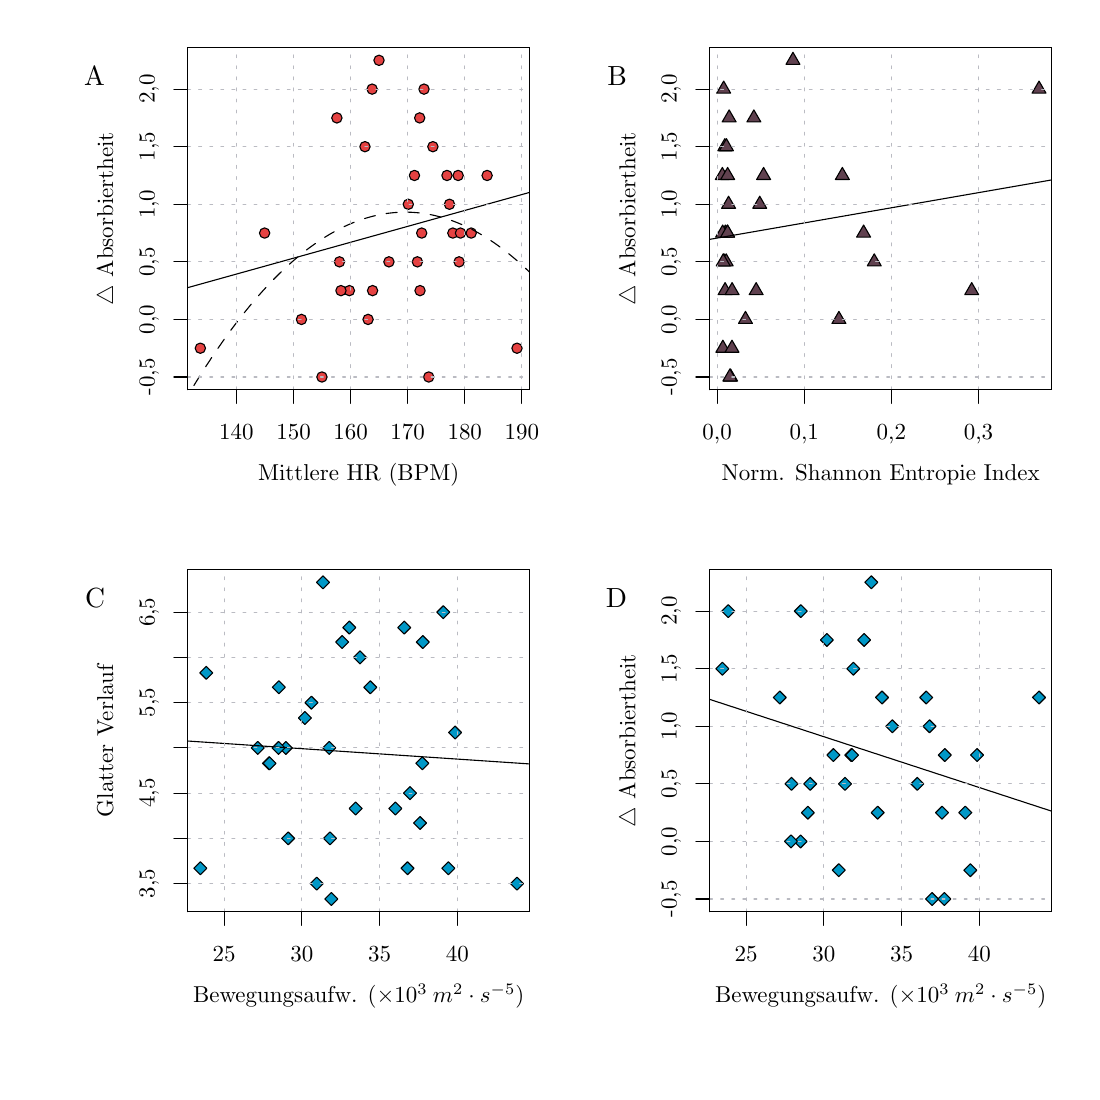
\begin{tikzpicture}[x=1pt,y=1pt]
\definecolor{fillColor}{RGB}{255,255,255}
\path[use as bounding box,fill=fillColor,fill opacity=0.00] (0,0) rectangle (377.25,377.25);
\begin{scope}
\path[clip] ( 57.82,246.44) rectangle (181.40,370.02);
\definecolor{drawColor}{RGB}{0,0,0}
\definecolor{fillColor}{RGB}{229,66,66}

\path[draw=drawColor,line width= 0.4pt,line join=round,line cap=round,fill=fillColor] (116.25,282.23) circle (  1.87);

\path[draw=drawColor,line width= 0.4pt,line join=round,line cap=round,fill=fillColor] (155.55,323.84) circle (  1.87);

\path[draw=drawColor,line width= 0.4pt,line join=round,line cap=round,fill=fillColor] (160.27,303.03) circle (  1.87);

\path[draw=drawColor,line width= 0.4pt,line join=round,line cap=round,fill=fillColor] ( 85.62,303.03) circle (  1.87);

\path[draw=drawColor,line width= 0.4pt,line join=round,line cap=round,fill=fillColor] (137.53,313.43) circle (  1.87);

\path[draw=drawColor,line width= 0.4pt,line join=round,line cap=round,fill=fillColor] (123.00,271.82) circle (  1.87);

\path[draw=drawColor,line width= 0.4pt,line join=round,line cap=round,fill=fillColor] (126.96,365.45) circle (  1.87);

\path[draw=drawColor,line width= 0.4pt,line join=round,line cap=round,fill=fillColor] (155.89,292.63) circle (  1.87);

\path[draw=drawColor,line width= 0.4pt,line join=round,line cap=round,fill=fillColor] (176.82,261.42) circle (  1.87);

\path[draw=drawColor,line width= 0.4pt,line join=round,line cap=round,fill=fillColor] (153.63,303.03) circle (  1.87);

\path[draw=drawColor,line width= 0.4pt,line join=round,line cap=round,fill=fillColor] (166.02,323.84) circle (  1.87);

\path[draw=drawColor,line width= 0.4pt,line join=round,line cap=round,fill=fillColor] (141.66,344.64) circle (  1.87);

\path[draw=drawColor,line width= 0.4pt,line join=round,line cap=round,fill=fillColor] (141.78,282.23) circle (  1.87);

\path[draw=drawColor,line width= 0.4pt,line join=round,line cap=round,fill=fillColor] (130.54,292.63) circle (  1.87);

\path[draw=drawColor,line width= 0.4pt,line join=round,line cap=round,fill=fillColor] ( 98.93,271.82) circle (  1.87);

\path[draw=drawColor,line width= 0.4pt,line join=round,line cap=round,fill=fillColor] (146.42,334.24) circle (  1.87);

\path[draw=drawColor,line width= 0.4pt,line join=round,line cap=round,fill=fillColor] (144.92,251.02) circle (  1.87);

\path[draw=drawColor,line width= 0.4pt,line join=round,line cap=round,fill=fillColor] (111.73,344.64) circle (  1.87);

\path[draw=drawColor,line width= 0.4pt,line join=round,line cap=round,fill=fillColor] (113.20,282.23) circle (  1.87);

\path[draw=drawColor,line width= 0.4pt,line join=round,line cap=round,fill=fillColor] (139.76,323.84) circle (  1.87);

\path[draw=drawColor,line width= 0.4pt,line join=round,line cap=round,fill=fillColor] (121.88,334.24) circle (  1.87);

\path[draw=drawColor,line width= 0.4pt,line join=round,line cap=round,fill=fillColor] (124.47,355.04) circle (  1.87);

\path[draw=drawColor,line width= 0.4pt,line join=round,line cap=round,fill=fillColor] (124.63,282.23) circle (  1.87);

\path[draw=drawColor,line width= 0.4pt,line join=round,line cap=round,fill=fillColor] (112.66,292.63) circle (  1.87);

\path[draw=drawColor,line width= 0.4pt,line join=round,line cap=round,fill=fillColor] (142.38,303.03) circle (  1.87);

\path[draw=drawColor,line width= 0.4pt,line join=round,line cap=round,fill=fillColor] (151.51,323.84) circle (  1.87);

\path[draw=drawColor,line width= 0.4pt,line join=round,line cap=round,fill=fillColor] (106.33,251.02) circle (  1.87);

\path[draw=drawColor,line width= 0.4pt,line join=round,line cap=round,fill=fillColor] (152.42,313.43) circle (  1.87);

\path[draw=drawColor,line width= 0.4pt,line join=round,line cap=round,fill=fillColor] (140.82,292.63) circle (  1.87);

\path[draw=drawColor,line width= 0.4pt,line join=round,line cap=round,fill=fillColor] (143.22,355.04) circle (  1.87);

\path[draw=drawColor,line width= 0.4pt,line join=round,line cap=round,fill=fillColor] ( 62.39,261.42) circle (  1.87);

\path[draw=drawColor,line width= 0.4pt,line join=round,line cap=round,fill=fillColor] (156.39,303.03) circle (  1.87);
\end{scope}
\begin{scope}
\path[clip] (  0.00,  0.00) rectangle (377.25,377.25);
\definecolor{drawColor}{RGB}{0,0,0}

\path[draw=drawColor,line width= 0.4pt,line join=round,line cap=round] ( 75.45,246.44) -- (178.56,246.44);

\path[draw=drawColor,line width= 0.4pt,line join=round,line cap=round] ( 75.45,246.44) -- ( 75.45,241.46);

\path[draw=drawColor,line width= 0.4pt,line join=round,line cap=round] ( 96.07,246.44) -- ( 96.07,241.46);

\path[draw=drawColor,line width= 0.4pt,line join=round,line cap=round] (116.69,246.44) -- (116.69,241.46);

\path[draw=drawColor,line width= 0.4pt,line join=round,line cap=round] (137.31,246.44) -- (137.31,241.46);

\path[draw=drawColor,line width= 0.4pt,line join=round,line cap=round] (157.94,246.44) -- (157.94,241.46);

\path[draw=drawColor,line width= 0.4pt,line join=round,line cap=round] (178.56,246.44) -- (178.56,241.46);

\node[text=drawColor,anchor=base,inner sep=0pt, outer sep=0pt, scale=  0.83] at ( 75.45,228.51) {140};

\node[text=drawColor,anchor=base,inner sep=0pt, outer sep=0pt, scale=  0.83] at ( 96.07,228.51) {150};

\node[text=drawColor,anchor=base,inner sep=0pt, outer sep=0pt, scale=  0.83] at (116.69,228.51) {160};

\node[text=drawColor,anchor=base,inner sep=0pt, outer sep=0pt, scale=  0.83] at (137.31,228.51) {170};

\node[text=drawColor,anchor=base,inner sep=0pt, outer sep=0pt, scale=  0.83] at (157.94,228.51) {180};

\node[text=drawColor,anchor=base,inner sep=0pt, outer sep=0pt, scale=  0.83] at (178.56,228.51) {190};

\path[draw=drawColor,line width= 0.4pt,line join=round,line cap=round] ( 57.82,251.02) -- ( 57.82,355.04);

\path[draw=drawColor,line width= 0.4pt,line join=round,line cap=round] ( 57.82,251.02) -- ( 52.84,251.02);

\path[draw=drawColor,line width= 0.4pt,line join=round,line cap=round] ( 57.82,271.82) -- ( 52.84,271.82);

\path[draw=drawColor,line width= 0.4pt,line join=round,line cap=round] ( 57.82,292.63) -- ( 52.84,292.63);

\path[draw=drawColor,line width= 0.4pt,line join=round,line cap=round] ( 57.82,313.43) -- ( 52.84,313.43);

\path[draw=drawColor,line width= 0.4pt,line join=round,line cap=round] ( 57.82,334.24) -- ( 52.84,334.24);

\path[draw=drawColor,line width= 0.4pt,line join=round,line cap=round] ( 57.82,355.04) -- ( 52.84,355.04);

\node[text=drawColor,rotate= 90.00,anchor=base,inner sep=0pt, outer sep=0pt, scale=  0.83] at ( 45.86,251.02) {-0,5};

\node[text=drawColor,rotate= 90.00,anchor=base,inner sep=0pt, outer sep=0pt, scale=  0.83] at ( 45.86,271.82) {0,0};

\node[text=drawColor,rotate= 90.00,anchor=base,inner sep=0pt, outer sep=0pt, scale=  0.83] at ( 45.86,292.63) {0,5};

\node[text=drawColor,rotate= 90.00,anchor=base,inner sep=0pt, outer sep=0pt, scale=  0.83] at ( 45.86,313.43) {1,0};

\node[text=drawColor,rotate= 90.00,anchor=base,inner sep=0pt, outer sep=0pt, scale=  0.83] at ( 45.86,334.24) {1,5};

\node[text=drawColor,rotate= 90.00,anchor=base,inner sep=0pt, outer sep=0pt, scale=  0.83] at ( 45.86,355.04) {2,0};

\path[draw=drawColor,line width= 0.4pt,line join=round,line cap=round] ( 57.82,246.44) --
	(181.40,246.44) --
	(181.40,370.02) --
	( 57.82,370.02) --
	( 57.82,246.44);
\end{scope}
\begin{scope}
\path[clip] (  0.00,188.62) rectangle (188.62,377.25);
\definecolor{drawColor}{RGB}{0,0,0}

\node[text=drawColor,anchor=base,inner sep=0pt, outer sep=0pt, scale=  0.83] at (119.61,213.57) {Mittlere HR (BPM)};

\node[text=drawColor,rotate= 90.00,anchor=base,inner sep=0pt, outer sep=0pt, scale=  0.83] at ( 30.92,308.23) {$\bigtriangleup$ Absorbiertheit};
\end{scope}
\begin{scope}
\path[clip] ( 57.82,246.44) rectangle (181.40,370.02);
\definecolor{drawColor}{RGB}{0,0,0}

\path[draw=drawColor,line width= 0.4pt,line join=round,line cap=round] ( 57.82,283.30) -- (181.40,317.73);

\path[draw=drawColor,line width= 0.4pt,dash pattern=on 4pt off 4pt ,line join=round,line cap=round] ( 34.20,198.31) --
	( 35.23,200.57) --
	( 36.26,202.80) --
	( 37.30,205.01) --
	( 38.33,207.19) --
	( 39.36,209.35) --
	( 40.39,211.49) --
	( 41.42,213.61) --
	( 42.45,215.70) --
	( 43.48,217.77) --
	( 44.51,219.82) --
	( 45.54,221.85) --
	( 46.58,223.85) --
	( 47.61,225.83) --
	( 48.64,227.78) --
	( 49.67,229.72) --
	( 50.70,231.63) --
	( 51.73,233.52) --
	( 52.76,235.38) --
	( 53.79,237.22) --
	( 54.82,239.04) --
	( 55.86,240.84) --
	( 56.89,242.61) --
	( 57.92,244.36) --
	( 58.95,246.09) --
	( 59.98,247.80) --
	( 61.01,249.48) --
	( 62.04,251.14) --
	( 63.07,252.77) --
	( 64.10,254.39) --
	( 65.14,255.98) --
	( 66.17,257.55) --
	( 67.20,259.09) --
	( 68.23,260.61) --
	( 69.26,262.11) --
	( 70.29,263.59) --
	( 71.32,265.05) --
	( 72.35,266.48) --
	( 73.38,267.88) --
	( 74.42,269.27) --
	( 75.45,270.63) --
	( 76.48,271.97) --
	( 77.51,273.29) --
	( 78.54,274.58) --
	( 79.57,275.85) --
	( 80.60,277.10) --
	( 81.63,278.33) --
	( 82.66,279.53) --
	( 83.70,280.71) --
	( 84.73,281.87) --
	( 85.76,283.00) --
	( 86.79,284.11) --
	( 87.82,285.20) --
	( 88.85,286.27) --
	( 89.88,287.31) --
	( 90.91,288.33) --
	( 91.94,289.33) --
	( 92.98,290.30) --
	( 94.01,291.25) --
	( 95.04,292.18) --
	( 96.07,293.08) --
	( 97.10,293.97) --
	( 98.13,294.83) --
	( 99.16,295.66) --
	(100.19,296.48) --
	(101.22,297.27) --
	(102.26,298.04) --
	(103.29,298.78) --
	(104.32,299.51) --
	(105.35,300.21) --
	(106.38,300.88) --
	(107.41,301.54) --
	(108.44,302.17) --
	(109.47,302.78) --
	(110.50,303.36) --
	(111.54,303.93) --
	(112.57,304.47) --
	(113.60,304.99) --
	(114.63,305.48) --
	(115.66,305.95) --
	(116.69,306.40) --
	(117.72,306.83) --
	(118.75,307.23) --
	(119.78,307.61) --
	(120.82,307.97) --
	(121.85,308.30) --
	(122.88,308.61) --
	(123.91,308.90) --
	(124.94,309.17) --
	(125.97,309.41) --
	(127.00,309.63) --
	(128.03,309.83) --
	(129.06,310.00) --
	(130.10,310.16) --
	(131.13,310.28) --
	(132.16,310.39) --
	(133.19,310.47) --
	(134.22,310.53) --
	(135.25,310.57) --
	(136.28,310.59) --
	(137.31,310.58) --
	(138.34,310.55) --
	(139.38,310.49) --
	(140.41,310.42) --
	(141.44,310.32) --
	(142.47,310.19) --
	(143.50,310.05) --
	(144.53,309.88) --
	(145.56,309.69) --
	(146.59,309.48) --
	(147.62,309.24) --
	(148.66,308.98) --
	(149.69,308.70) --
	(150.72,308.39) --
	(151.75,308.07) --
	(152.78,307.72) --
	(153.81,307.34) --
	(154.84,306.94) --
	(155.87,306.53) --
	(156.90,306.08) --
	(157.94,305.62) --
	(158.97,305.13) --
	(160.00,304.62) --
	(161.03,304.09) --
	(162.06,303.53) --
	(163.09,302.95) --
	(164.12,302.35) --
	(165.15,301.72) --
	(166.18,301.08) --
	(167.21,300.41) --
	(168.25,299.71) --
	(169.28,299.00) --
	(170.31,298.26) --
	(171.34,297.49) --
	(172.37,296.71) --
	(173.40,295.90) --
	(174.43,295.07) --
	(175.46,294.22) --
	(176.49,293.34) --
	(177.53,292.44) --
	(178.56,291.52) --
	(179.59,290.58) --
	(180.62,289.61) --
	(181.65,288.62) --
	(182.68,287.61) --
	(183.71,286.57) --
	(184.74,285.51) --
	(185.77,284.43) --
	(186.81,283.32) --
	(187.84,282.20) --
	(188.87,281.05) --
	(189.90,279.87) --
	(190.93,278.68) --
	(191.96,277.46) --
	(192.99,276.22) --
	(194.02,274.95) --
	(195.05,273.66) --
	(196.09,272.35) --
	(197.12,271.02) --
	(198.15,269.67) --
	(199.18,268.29);
\definecolor{drawColor}{RGB}{186,187,194}

\path[draw=drawColor,line width= 0.4pt,dash pattern=on 1pt off 3pt ,line join=round,line cap=round] ( 75.45,246.44) -- ( 75.45,370.02);

\path[draw=drawColor,line width= 0.4pt,dash pattern=on 1pt off 3pt ,line join=round,line cap=round] ( 96.07,246.44) -- ( 96.07,370.02);

\path[draw=drawColor,line width= 0.4pt,dash pattern=on 1pt off 3pt ,line join=round,line cap=round] (116.69,246.44) -- (116.69,370.02);

\path[draw=drawColor,line width= 0.4pt,dash pattern=on 1pt off 3pt ,line join=round,line cap=round] (137.31,246.44) -- (137.31,370.02);

\path[draw=drawColor,line width= 0.4pt,dash pattern=on 1pt off 3pt ,line join=round,line cap=round] (157.94,246.44) -- (157.94,370.02);

\path[draw=drawColor,line width= 0.4pt,dash pattern=on 1pt off 3pt ,line join=round,line cap=round] (178.56,246.44) -- (178.56,370.02);

\path[draw=drawColor,line width= 0.4pt,dash pattern=on 1pt off 3pt ,line join=round,line cap=round] ( 57.82,251.02) -- (181.40,251.02);

\path[draw=drawColor,line width= 0.4pt,dash pattern=on 1pt off 3pt ,line join=round,line cap=round] ( 57.82,271.82) -- (181.40,271.82);

\path[draw=drawColor,line width= 0.4pt,dash pattern=on 1pt off 3pt ,line join=round,line cap=round] ( 57.82,292.63) -- (181.40,292.63);

\path[draw=drawColor,line width= 0.4pt,dash pattern=on 1pt off 3pt ,line join=round,line cap=round] ( 57.82,313.43) -- (181.40,313.43);

\path[draw=drawColor,line width= 0.4pt,dash pattern=on 1pt off 3pt ,line join=round,line cap=round] ( 57.82,334.24) -- (181.40,334.24);

\path[draw=drawColor,line width= 0.4pt,dash pattern=on 1pt off 3pt ,line join=round,line cap=round] ( 57.82,355.04) -- (181.40,355.04);
\end{scope}
\begin{scope}
\path[clip] (  0.00,  0.00) rectangle (377.25,377.25);
\definecolor{drawColor}{RGB}{0,0,0}

\path[draw=drawColor,line width= 0.4pt,line join=round,line cap=round] ( 57.82,246.44) --
	(181.40,246.44) --
	(181.40,370.02) --
	( 57.82,370.02) --
	( 57.82,246.44);

\node[text=drawColor,anchor=base east,inner sep=0pt, outer sep=0pt, scale=  1.00] at ( 27.94,356.44) {A};
\end{scope}
\begin{scope}
\path[clip] (246.44,246.44) rectangle (370.02,370.02);
\definecolor{drawColor}{RGB}{0,0,0}
\definecolor{fillColor}{RGB}{96,65,79}

\path[draw=drawColor,line width= 0.4pt,line join=round,line cap=round,fill=fillColor] (252.01,285.13) --
	(254.52,280.77) --
	(249.49,280.77) --
	cycle;

\path[draw=drawColor,line width= 0.4pt,line join=round,line cap=round,fill=fillColor] (294.38,326.74) --
	(296.90,322.38) --
	(291.87,322.38) --
	cycle;

\path[draw=drawColor,line width= 0.4pt,line join=round,line cap=round,fill=fillColor] (252.10,305.93) --
	(254.62,301.58) --
	(249.59,301.58) --
	cycle;

\path[draw=drawColor,line width= 0.4pt,line join=round,line cap=round,fill=fillColor] (252.84,305.93) --
	(255.36,301.58) --
	(250.33,301.58) --
	cycle;

\path[draw=drawColor,line width= 0.4pt,line join=round,line cap=round,fill=fillColor] (264.53,316.34) --
	(267.04,311.98) --
	(262.01,311.98) --
	cycle;

\path[draw=drawColor,line width= 0.4pt,line join=round,line cap=round,fill=fillColor] (293.14,274.73) --
	(295.66,270.37) --
	(290.63,270.37) --
	cycle;

\path[draw=drawColor,line width= 0.4pt,line join=round,line cap=round,fill=fillColor] (276.54,368.35) --
	(279.05,363.99) --
	(274.02,363.99) --
	cycle;

\path[draw=drawColor,line width= 0.4pt,line join=round,line cap=round,fill=fillColor] (251.64,295.53) --
	(254.15,291.18) --
	(249.12,291.18) --
	cycle;

\path[draw=drawColor,line width= 0.4pt,line join=round,line cap=round,fill=fillColor] (251.21,264.32) --
	(253.72,259.97) --
	(248.69,259.97) --
	cycle;

\path[draw=drawColor,line width= 0.4pt,line join=round,line cap=round,fill=fillColor] (302.06,305.93) --
	(304.57,301.58) --
	(299.54,301.58) --
	cycle;

\path[draw=drawColor,line width= 0.4pt,line join=round,line cap=round,fill=fillColor] (265.92,326.74) --
	(268.44,322.38) --
	(263.41,322.38) --
	cycle;

\path[draw=drawColor,line width= 0.4pt,line join=round,line cap=round,fill=fillColor] (262.41,347.54) --
	(264.92,343.19) --
	(259.89,343.19) --
	cycle;

\path[draw=drawColor,line width= 0.4pt,line join=round,line cap=round,fill=fillColor] (263.23,285.13) --
	(265.75,280.77) --
	(260.72,280.77) --
	cycle;

\path[draw=drawColor,line width= 0.4pt,line join=round,line cap=round,fill=fillColor] (252.40,295.53) --
	(254.92,291.18) --
	(249.89,291.18) --
	cycle;

\path[draw=drawColor,line width= 0.4pt,line join=round,line cap=round,fill=fillColor] (259.37,274.73) --
	(261.89,270.37) --
	(256.86,270.37) --
	cycle;

\path[draw=drawColor,line width= 0.4pt,line join=round,line cap=round,fill=fillColor] (251.91,337.14) --
	(254.42,332.79) --
	(249.39,332.79) --
	cycle;

\path[draw=drawColor,line width= 0.4pt,line join=round,line cap=round,fill=fillColor] (253.99,253.92) --
	(256.50,249.57) --
	(251.47,249.57) --
	cycle;

\path[draw=drawColor,line width= 0.4pt,line join=round,line cap=round,fill=fillColor] (253.48,347.54) --
	(255.99,343.19) --
	(250.96,343.19) --
	cycle;

\path[draw=drawColor,line width= 0.4pt,line join=round,line cap=round,fill=fillColor] (341.12,285.13) --
	(343.64,280.77) --
	(338.61,280.77) --
	cycle;

\path[draw=drawColor,line width= 0.4pt,line join=round,line cap=round,fill=fillColor] (251.02,326.74) --
	(253.53,322.38) --
	(248.50,322.38) --
	cycle;

\path[draw=drawColor,line width= 0.4pt,line join=round,line cap=round,fill=fillColor] (252.50,337.14) --
	(255.01,332.79) --
	(249.98,332.79) --
	cycle;

\path[draw=drawColor,line width= 0.4pt,line join=round,line cap=round,fill=fillColor] (365.45,357.95) --
	(367.96,353.59) --
	(362.93,353.59) --
	cycle;

\path[draw=drawColor,line width= 0.4pt,line join=round,line cap=round,fill=fillColor] (254.54,285.13) --
	(257.05,280.77) --
	(252.02,280.77) --
	cycle;

\path[draw=drawColor,line width= 0.4pt,line join=round,line cap=round,fill=fillColor] (305.91,295.53) --
	(308.43,291.18) --
	(303.40,291.18) --
	cycle;

\path[draw=drawColor,line width= 0.4pt,line join=round,line cap=round,fill=fillColor] (251.13,305.93) --
	(253.64,301.58) --
	(248.61,301.58) --
	cycle;

\path[draw=drawColor,line width= 0.4pt,line join=round,line cap=round,fill=fillColor] (252.93,326.74) --
	(255.45,322.38) --
	(250.42,322.38) --
	cycle;

\path[draw=drawColor,line width= 0.4pt,line join=round,line cap=round,fill=fillColor] (253.74,253.92) --
	(256.26,249.57) --
	(251.22,249.57) --
	cycle;

\path[draw=drawColor,line width= 0.4pt,line join=round,line cap=round,fill=fillColor] (253.27,316.34) --
	(255.78,311.98) --
	(250.75,311.98) --
	cycle;

\path[draw=drawColor,line width= 0.4pt,line join=round,line cap=round,fill=fillColor] (251.33,295.53) --
	(253.84,291.18) --
	(248.81,291.18) --
	cycle;

\path[draw=drawColor,line width= 0.4pt,line join=round,line cap=round,fill=fillColor] (251.50,357.95) --
	(254.01,353.59) --
	(248.98,353.59) --
	cycle;

\path[draw=drawColor,line width= 0.4pt,line join=round,line cap=round,fill=fillColor] (254.50,264.32) --
	(257.02,259.97) --
	(251.99,259.97) --
	cycle;

\path[draw=drawColor,line width= 0.4pt,line join=round,line cap=round,fill=fillColor] (252.91,305.93) --
	(255.43,301.58) --
	(250.40,301.58) --
	cycle;
\end{scope}
\begin{scope}
\path[clip] (  0.00,  0.00) rectangle (377.25,377.25);
\definecolor{drawColor}{RGB}{0,0,0}

\path[draw=drawColor,line width= 0.4pt,line join=round,line cap=round] (249.12,246.44) -- (343.60,246.44);

\path[draw=drawColor,line width= 0.4pt,line join=round,line cap=round] (249.12,246.44) -- (249.12,241.46);

\path[draw=drawColor,line width= 0.4pt,line join=round,line cap=round] (280.61,246.44) -- (280.61,241.46);

\path[draw=drawColor,line width= 0.4pt,line join=round,line cap=round] (312.11,246.44) -- (312.11,241.46);

\path[draw=drawColor,line width= 0.4pt,line join=round,line cap=round] (343.60,246.44) -- (343.60,241.46);

\node[text=drawColor,anchor=base,inner sep=0pt, outer sep=0pt, scale=  0.83] at (249.12,228.51) {0,0};

\node[text=drawColor,anchor=base,inner sep=0pt, outer sep=0pt, scale=  0.83] at (280.61,228.51) {0,1};

\node[text=drawColor,anchor=base,inner sep=0pt, outer sep=0pt, scale=  0.83] at (312.11,228.51) {0,2};

\node[text=drawColor,anchor=base,inner sep=0pt, outer sep=0pt, scale=  0.83] at (343.60,228.51) {0,3};

\path[draw=drawColor,line width= 0.4pt,line join=round,line cap=round] (246.44,251.02) -- (246.44,355.04);

\path[draw=drawColor,line width= 0.4pt,line join=round,line cap=round] (246.44,251.02) -- (241.46,251.02);

\path[draw=drawColor,line width= 0.4pt,line join=round,line cap=round] (246.44,271.82) -- (241.46,271.82);

\path[draw=drawColor,line width= 0.4pt,line join=round,line cap=round] (246.44,292.63) -- (241.46,292.63);

\path[draw=drawColor,line width= 0.4pt,line join=round,line cap=round] (246.44,313.43) -- (241.46,313.43);

\path[draw=drawColor,line width= 0.4pt,line join=round,line cap=round] (246.44,334.24) -- (241.46,334.24);

\path[draw=drawColor,line width= 0.4pt,line join=round,line cap=round] (246.44,355.04) -- (241.46,355.04);

\node[text=drawColor,rotate= 90.00,anchor=base,inner sep=0pt, outer sep=0pt, scale=  0.83] at (234.49,251.02) {-0,5};

\node[text=drawColor,rotate= 90.00,anchor=base,inner sep=0pt, outer sep=0pt, scale=  0.83] at (234.49,271.82) {0,0};

\node[text=drawColor,rotate= 90.00,anchor=base,inner sep=0pt, outer sep=0pt, scale=  0.83] at (234.49,292.63) {0,5};

\node[text=drawColor,rotate= 90.00,anchor=base,inner sep=0pt, outer sep=0pt, scale=  0.83] at (234.49,313.43) {1,0};

\node[text=drawColor,rotate= 90.00,anchor=base,inner sep=0pt, outer sep=0pt, scale=  0.83] at (234.49,334.24) {1,5};

\node[text=drawColor,rotate= 90.00,anchor=base,inner sep=0pt, outer sep=0pt, scale=  0.83] at (234.49,355.04) {2,0};

\path[draw=drawColor,line width= 0.4pt,line join=round,line cap=round] (246.44,246.44) --
	(370.02,246.44) --
	(370.02,370.02) --
	(246.44,370.02) --
	(246.44,246.44);
\end{scope}
\begin{scope}
\path[clip] (188.62,188.62) rectangle (377.25,377.25);
\definecolor{drawColor}{RGB}{0,0,0}

\node[text=drawColor,anchor=base,inner sep=0pt, outer sep=0pt, scale=  0.83] at (308.23,213.57) {Norm. Shannon Entropie Index};

\node[text=drawColor,rotate= 90.00,anchor=base,inner sep=0pt, outer sep=0pt, scale=  0.83] at (219.55,308.23) {$\bigtriangleup$ Absorbiertheit};
\end{scope}
\begin{scope}
\path[clip] (246.44,246.44) rectangle (370.02,370.02);
\definecolor{drawColor}{RGB}{0,0,0}

\path[draw=drawColor,line width= 0.4pt,line join=round,line cap=round] (246.44,300.75) -- (370.02,322.23);
\definecolor{drawColor}{RGB}{186,187,194}

\path[draw=drawColor,line width= 0.4pt,dash pattern=on 1pt off 3pt ,line join=round,line cap=round] (249.12,246.44) -- (249.12,370.02);

\path[draw=drawColor,line width= 0.4pt,dash pattern=on 1pt off 3pt ,line join=round,line cap=round] (280.61,246.44) -- (280.61,370.02);

\path[draw=drawColor,line width= 0.4pt,dash pattern=on 1pt off 3pt ,line join=round,line cap=round] (312.11,246.44) -- (312.11,370.02);

\path[draw=drawColor,line width= 0.4pt,dash pattern=on 1pt off 3pt ,line join=round,line cap=round] (343.60,246.44) -- (343.60,370.02);

\path[draw=drawColor,line width= 0.4pt,dash pattern=on 1pt off 3pt ,line join=round,line cap=round] (246.44,251.02) -- (370.02,251.02);

\path[draw=drawColor,line width= 0.4pt,dash pattern=on 1pt off 3pt ,line join=round,line cap=round] (246.44,271.82) -- (370.02,271.82);

\path[draw=drawColor,line width= 0.4pt,dash pattern=on 1pt off 3pt ,line join=round,line cap=round] (246.44,292.63) -- (370.02,292.63);

\path[draw=drawColor,line width= 0.4pt,dash pattern=on 1pt off 3pt ,line join=round,line cap=round] (246.44,313.43) -- (370.02,313.43);

\path[draw=drawColor,line width= 0.4pt,dash pattern=on 1pt off 3pt ,line join=round,line cap=round] (246.44,334.24) -- (370.02,334.24);

\path[draw=drawColor,line width= 0.4pt,dash pattern=on 1pt off 3pt ,line join=round,line cap=round] (246.44,355.04) -- (370.02,355.04);
\end{scope}
\begin{scope}
\path[clip] (  0.00,  0.00) rectangle (377.25,377.25);
\definecolor{drawColor}{RGB}{0,0,0}

\path[draw=drawColor,line width= 0.4pt,line join=round,line cap=round] (246.44,246.44) --
	(370.02,246.44) --
	(370.02,370.02) --
	(246.44,370.02) --
	(246.44,246.44);

\node[text=drawColor,anchor=base east,inner sep=0pt, outer sep=0pt, scale=  1.00] at (216.56,356.44) {B};
\end{scope}
\begin{scope}
\path[clip] ( 57.82, 57.82) rectangle (181.40,181.40);
\definecolor{drawColor}{RGB}{0,0,0}
\definecolor{fillColor}{RGB}{0,152,199}

\path[draw=drawColor,line width= 0.4pt,line join=round,line cap=round,fill=fillColor] ( 93.29,114.65) --
	( 95.64,116.99) --
	( 93.29,119.33) --
	( 90.95,116.99) --
	cycle;

\path[draw=drawColor,line width= 0.4pt,line join=round,line cap=round,fill=fillColor] (136.05,158.13) --
	(138.39,160.47) --
	(136.05,162.81) --
	(133.71,160.47) --
	cycle;

\path[draw=drawColor,line width= 0.4pt,line join=round,line cap=round,fill=fillColor] (102.53,131.00) --
	(104.87,133.34) --
	(102.53,135.68) --
	(100.19,133.34) --
	cycle;

\path[draw=drawColor,line width= 0.4pt,line join=round,line cap=round,fill=fillColor] (142.78,152.90) --
	(145.12,155.24) --
	(142.78,157.58) --
	(140.44,155.24) --
	cycle;

\path[draw=drawColor,line width= 0.4pt,line join=round,line cap=round,fill=fillColor] (123.80,136.56) --
	(126.14,138.90) --
	(123.80,141.24) --
	(121.46,138.90) --
	cycle;

\path[draw=drawColor,line width= 0.4pt,line join=round,line cap=round,fill=fillColor] ( 90.66,114.65) --
	( 93.00,116.99) --
	( 90.66,119.33) --
	( 88.32,116.99) --
	cycle;

\path[draw=drawColor,line width= 0.4pt,line join=round,line cap=round,fill=fillColor] (116.23,158.13) --
	(118.57,160.47) --
	(116.23,162.81) --
	(113.89,160.47) --
	cycle;

\path[draw=drawColor,line width= 0.4pt,line join=round,line cap=round,fill=fillColor] (132.85, 92.75) --
	(135.19, 95.09) --
	(132.85, 97.43) --
	(130.51, 95.09) --
	cycle;

\path[draw=drawColor,line width= 0.4pt,line join=round,line cap=round,fill=fillColor] (152.01, 71.17) --
	(154.35, 73.51) --
	(152.01, 75.85) --
	(149.67, 73.51) --
	cycle;

\path[draw=drawColor,line width= 0.4pt,line join=round,line cap=round,fill=fillColor] (108.97,114.65) --
	(111.31,116.99) --
	(108.97,119.33) --
	(106.63,116.99) --
	cycle;

\path[draw=drawColor,line width= 0.4pt,line join=round,line cap=round,fill=fillColor] (176.82, 65.61) --
	(179.16, 67.95) --
	(176.82, 70.29) --
	(174.48, 67.95) --
	cycle;

\path[draw=drawColor,line width= 0.4pt,line join=round,line cap=round,fill=fillColor] (113.63,152.90) --
	(115.97,155.24) --
	(113.63,157.58) --
	(111.29,155.24) --
	cycle;

\path[draw=drawColor,line width= 0.4pt,line join=round,line cap=round,fill=fillColor] (150.18,163.69) --
	(152.52,166.03) --
	(150.18,168.37) --
	(147.84,166.03) --
	cycle;

\path[draw=drawColor,line width= 0.4pt,line join=round,line cap=round,fill=fillColor] (106.72,174.48) --
	(109.06,176.82) --
	(106.72,179.16) --
	(104.38,176.82) --
	cycle;

\path[draw=drawColor,line width= 0.4pt,line join=round,line cap=round,fill=fillColor] ( 87.20,109.09) --
	( 89.54,111.43) --
	( 87.20,113.77) --
	( 84.85,111.43) --
	cycle;

\path[draw=drawColor,line width= 0.4pt,line join=round,line cap=round,fill=fillColor] (109.73, 60.05) --
	(112.07, 62.39) --
	(109.73, 64.73) --
	(107.39, 62.39) --
	cycle;

\path[draw=drawColor,line width= 0.4pt,line join=round,line cap=round,fill=fillColor] (138.16, 98.30) --
	(140.50,100.64) --
	(138.16,102.99) --
	(135.82,100.64) --
	cycle;

\path[draw=drawColor,line width= 0.4pt,line join=round,line cap=round,fill=fillColor] (100.17,125.44) --
	(102.51,127.78) --
	(100.17,130.12) --
	( 97.83,127.78) --
	cycle;

\path[draw=drawColor,line width= 0.4pt,line join=round,line cap=round,fill=fillColor] (118.51, 92.75) --
	(120.85, 95.09) --
	(118.51, 97.43) --
	(116.17, 95.09) --
	cycle;

\path[draw=drawColor,line width= 0.4pt,line join=round,line cap=round,fill=fillColor] ( 83.14,114.65) --
	( 85.48,116.99) --
	( 83.14,119.33) --
	( 80.80,116.99) --
	cycle;

\path[draw=drawColor,line width= 0.4pt,line join=round,line cap=round,fill=fillColor] ( 62.39, 71.17) --
	( 64.73, 73.51) --
	( 62.39, 75.85) --
	( 60.05, 73.51) --
	cycle;

\path[draw=drawColor,line width= 0.4pt,line join=round,line cap=round,fill=fillColor] ( 90.76,136.56) --
	( 93.10,138.90) --
	( 90.76,141.24) --
	( 88.42,138.90) --
	cycle;

\path[draw=drawColor,line width= 0.4pt,line join=round,line cap=round,fill=fillColor] (141.78, 87.52) --
	(144.12, 89.86) --
	(141.78, 92.20) --
	(139.44, 89.86) --
	cycle;

\path[draw=drawColor,line width= 0.4pt,line join=round,line cap=round,fill=fillColor] ( 94.13, 81.96) --
	( 96.47, 84.30) --
	( 94.13, 86.64) --
	( 91.78, 84.30) --
	cycle;

\path[draw=drawColor,line width= 0.4pt,line join=round,line cap=round,fill=fillColor] (109.24, 81.96) --
	(111.58, 84.30) --
	(109.24, 86.64) --
	(106.90, 84.30) --
	cycle;

\path[draw=drawColor,line width= 0.4pt,line join=round,line cap=round,fill=fillColor] (120.08,147.34) --
	(122.42,149.68) --
	(120.08,152.03) --
	(117.74,149.68) --
	cycle;

\path[draw=drawColor,line width= 0.4pt,line join=round,line cap=round,fill=fillColor] (142.61,109.09) --
	(144.95,111.43) --
	(142.61,113.77) --
	(140.27,111.43) --
	cycle;

\path[draw=drawColor,line width= 0.4pt,line join=round,line cap=round,fill=fillColor] (137.25, 71.17) --
	(139.59, 73.51) --
	(137.25, 75.85) --
	(134.91, 73.51) --
	cycle;

\path[draw=drawColor,line width= 0.4pt,line join=round,line cap=round,fill=fillColor] ( 87.39,109.09) --
	( 89.73,111.43) --
	( 87.39,113.77) --
	( 85.05,111.43) --
	cycle;

\path[draw=drawColor,line width= 0.4pt,line join=round,line cap=round,fill=fillColor] ( 64.54,141.79) --
	( 66.88,144.13) --
	( 64.54,146.47) --
	( 62.20,144.13) --
	cycle;

\path[draw=drawColor,line width= 0.4pt,line join=round,line cap=round,fill=fillColor] (104.47, 65.61) --
	(106.81, 67.95) --
	(104.47, 70.29) --
	(102.13, 67.95) --
	cycle;

\path[draw=drawColor,line width= 0.4pt,line join=round,line cap=round,fill=fillColor] (154.44,120.21) --
	(156.78,122.55) --
	(154.44,124.89) --
	(152.10,122.55) --
	cycle;
\end{scope}
\begin{scope}
\path[clip] (  0.00,  0.00) rectangle (377.25,377.25);
\definecolor{drawColor}{RGB}{0,0,0}

\path[draw=drawColor,line width= 0.4pt,line join=round,line cap=round] ( 71.00, 57.82) -- (155.29, 57.82);

\path[draw=drawColor,line width= 0.4pt,line join=round,line cap=round] ( 71.00, 57.82) -- ( 71.00, 52.84);

\path[draw=drawColor,line width= 0.4pt,line join=round,line cap=round] ( 99.10, 57.82) -- ( 99.10, 52.84);

\path[draw=drawColor,line width= 0.4pt,line join=round,line cap=round] (127.20, 57.82) -- (127.20, 52.84);

\path[draw=drawColor,line width= 0.4pt,line join=round,line cap=round] (155.29, 57.82) -- (155.29, 52.84);

\node[text=drawColor,anchor=base,inner sep=0pt, outer sep=0pt, scale=  0.83] at ( 71.00, 39.89) {25};

\node[text=drawColor,anchor=base,inner sep=0pt, outer sep=0pt, scale=  0.83] at ( 99.10, 39.89) {30};

\node[text=drawColor,anchor=base,inner sep=0pt, outer sep=0pt, scale=  0.83] at (127.20, 39.89) {35};

\node[text=drawColor,anchor=base,inner sep=0pt, outer sep=0pt, scale=  0.83] at (155.29, 39.89) {40};

\path[draw=drawColor,line width= 0.4pt,line join=round,line cap=round] ( 57.82, 67.95) -- ( 57.82,166.03);

\path[draw=drawColor,line width= 0.4pt,line join=round,line cap=round] ( 57.82, 67.95) -- ( 52.84, 67.95);

\path[draw=drawColor,line width= 0.4pt,line join=round,line cap=round] ( 57.82, 84.30) -- ( 52.84, 84.30);

\path[draw=drawColor,line width= 0.4pt,line join=round,line cap=round] ( 57.82,100.64) -- ( 52.84,100.64);

\path[draw=drawColor,line width= 0.4pt,line join=round,line cap=round] ( 57.82,116.99) -- ( 52.84,116.99);

\path[draw=drawColor,line width= 0.4pt,line join=round,line cap=round] ( 57.82,133.34) -- ( 52.84,133.34);

\path[draw=drawColor,line width= 0.4pt,line join=round,line cap=round] ( 57.82,149.68) -- ( 52.84,149.68);

\path[draw=drawColor,line width= 0.4pt,line join=round,line cap=round] ( 57.82,166.03) -- ( 52.84,166.03);

\node[text=drawColor,rotate= 90.00,anchor=base,inner sep=0pt, outer sep=0pt, scale=  0.83] at ( 45.86, 67.95) {3,5};

\node[text=drawColor,rotate= 90.00,anchor=base,inner sep=0pt, outer sep=0pt, scale=  0.83] at ( 45.86,100.64) {4,5};

\node[text=drawColor,rotate= 90.00,anchor=base,inner sep=0pt, outer sep=0pt, scale=  0.83] at ( 45.86,133.34) {5,5};

\node[text=drawColor,rotate= 90.00,anchor=base,inner sep=0pt, outer sep=0pt, scale=  0.83] at ( 45.86,166.03) {6,5};

\path[draw=drawColor,line width= 0.4pt,line join=round,line cap=round] ( 57.82, 57.82) --
	(181.40, 57.82) --
	(181.40,181.40) --
	( 57.82,181.40) --
	( 57.82, 57.82);
\end{scope}
\begin{scope}
\path[clip] (  0.00,  0.00) rectangle (188.62,188.62);
\definecolor{drawColor}{RGB}{0,0,0}

\node[text=drawColor,anchor=base,inner sep=0pt, outer sep=0pt, scale=  0.83] at (119.61, 24.95) {Bewegungsaufw. ($\times 10^3 \: m^2 \cdot s^{-5}$)};

\node[text=drawColor,rotate= 90.00,anchor=base,inner sep=0pt, outer sep=0pt, scale=  0.83] at ( 30.92,119.61) {Glatter Verlauf};
\end{scope}
\begin{scope}
\path[clip] ( 57.82, 57.82) rectangle (181.40,181.40);
\definecolor{drawColor}{RGB}{0,0,0}

\path[draw=drawColor,line width= 0.4pt,line join=round,line cap=round] ( 57.82,119.48) -- (181.40,111.20);
\definecolor{drawColor}{RGB}{186,187,194}

\path[draw=drawColor,line width= 0.4pt,dash pattern=on 1pt off 3pt ,line join=round,line cap=round] ( 71.00, 57.82) -- ( 71.00,181.40);

\path[draw=drawColor,line width= 0.4pt,dash pattern=on 1pt off 3pt ,line join=round,line cap=round] ( 99.10, 57.82) -- ( 99.10,181.40);

\path[draw=drawColor,line width= 0.4pt,dash pattern=on 1pt off 3pt ,line join=round,line cap=round] (127.20, 57.82) -- (127.20,181.40);

\path[draw=drawColor,line width= 0.4pt,dash pattern=on 1pt off 3pt ,line join=round,line cap=round] (155.29, 57.82) -- (155.29,181.40);

\path[draw=drawColor,line width= 0.4pt,dash pattern=on 1pt off 3pt ,line join=round,line cap=round] ( 57.82, 67.95) -- (181.40, 67.95);

\path[draw=drawColor,line width= 0.4pt,dash pattern=on 1pt off 3pt ,line join=round,line cap=round] ( 57.82, 84.30) -- (181.40, 84.30);

\path[draw=drawColor,line width= 0.4pt,dash pattern=on 1pt off 3pt ,line join=round,line cap=round] ( 57.82,100.64) -- (181.40,100.64);

\path[draw=drawColor,line width= 0.4pt,dash pattern=on 1pt off 3pt ,line join=round,line cap=round] ( 57.82,116.99) -- (181.40,116.99);

\path[draw=drawColor,line width= 0.4pt,dash pattern=on 1pt off 3pt ,line join=round,line cap=round] ( 57.82,133.34) -- (181.40,133.34);

\path[draw=drawColor,line width= 0.4pt,dash pattern=on 1pt off 3pt ,line join=round,line cap=round] ( 57.82,149.68) -- (181.40,149.68);

\path[draw=drawColor,line width= 0.4pt,dash pattern=on 1pt off 3pt ,line join=round,line cap=round] ( 57.82,166.03) -- (181.40,166.03);
\end{scope}
\begin{scope}
\path[clip] (  0.00,  0.00) rectangle (377.25,377.25);
\definecolor{drawColor}{RGB}{0,0,0}

\path[draw=drawColor,line width= 0.4pt,line join=round,line cap=round] ( 57.82, 57.82) --
	(181.40, 57.82) --
	(181.40,181.40) --
	( 57.82,181.40) --
	( 57.82, 57.82);

\node[text=drawColor,anchor=base east,inner sep=0pt, outer sep=0pt, scale=  1.00] at ( 27.94,167.82) {C};
\end{scope}
\begin{scope}
\path[clip] (246.44, 57.82) rectangle (370.02,181.40);
\definecolor{drawColor}{RGB}{0,0,0}
\definecolor{fillColor}{RGB}{0,152,199}

\path[draw=drawColor,line width= 0.4pt,line join=round,line cap=round,fill=fillColor] (281.92, 91.26) --
	(284.26, 93.60) --
	(281.92, 95.94) --
	(279.58, 93.60) --
	cycle;

\path[draw=drawColor,line width= 0.4pt,line join=round,line cap=round,fill=fillColor] (324.68,132.87) --
	(327.02,135.21) --
	(324.68,137.55) --
	(322.34,135.21) --
	cycle;

\path[draw=drawColor,line width= 0.4pt,line join=round,line cap=round,fill=fillColor] (291.15,112.07) --
	(293.49,114.41) --
	(291.15,116.75) --
	(288.81,114.41) --
	cycle;

\path[draw=drawColor,line width= 0.4pt,line join=round,line cap=round,fill=fillColor] (331.40,112.07) --
	(333.74,114.41) --
	(331.40,116.75) --
	(329.06,114.41) --
	cycle;

\path[draw=drawColor,line width= 0.4pt,line join=round,line cap=round,fill=fillColor] (312.43,122.47) --
	(314.77,124.81) --
	(312.43,127.15) --
	(310.09,124.81) --
	cycle;

\path[draw=drawColor,line width= 0.4pt,line join=round,line cap=round,fill=fillColor] (279.29, 80.86) --
	(281.63, 83.20) --
	(279.29, 85.54) --
	(276.95, 83.20) --
	cycle;

\path[draw=drawColor,line width= 0.4pt,line join=round,line cap=round,fill=fillColor] (304.86,174.48) --
	(307.20,176.82) --
	(304.86,179.16) --
	(302.52,176.82) --
	cycle;

\path[draw=drawColor,line width= 0.4pt,line join=round,line cap=round,fill=fillColor] (321.48,101.66) --
	(323.82,104.00) --
	(321.48,106.34) --
	(319.14,104.00) --
	cycle;

\path[draw=drawColor,line width= 0.4pt,line join=round,line cap=round,fill=fillColor] (340.63, 70.46) --
	(342.97, 72.80) --
	(340.63, 75.14) --
	(338.29, 72.80) --
	cycle;

\path[draw=drawColor,line width= 0.4pt,line join=round,line cap=round,fill=fillColor] (297.60,112.07) --
	(299.94,114.41) --
	(297.60,116.75) --
	(295.26,114.41) --
	cycle;

\path[draw=drawColor,line width= 0.4pt,line join=round,line cap=round,fill=fillColor] (365.45,132.87) --
	(367.79,135.21) --
	(365.45,137.55) --
	(363.10,135.21) --
	cycle;

\path[draw=drawColor,line width= 0.4pt,line join=round,line cap=round,fill=fillColor] (302.25,153.68) --
	(304.59,156.02) --
	(302.25,158.36) --
	(299.91,156.02) --
	cycle;

\path[draw=drawColor,line width= 0.4pt,line join=round,line cap=round,fill=fillColor] (338.80, 91.26) --
	(341.15, 93.60) --
	(338.80, 95.94) --
	(336.46, 93.60) --
	cycle;

\path[draw=drawColor,line width= 0.4pt,line join=round,line cap=round,fill=fillColor] (295.35,101.66) --
	(297.69,104.00) --
	(295.35,106.34) --
	(293.01,104.00) --
	cycle;

\path[draw=drawColor,line width= 0.4pt,line join=round,line cap=round,fill=fillColor] (275.82, 80.86) --
	(278.16, 83.20) --
	(275.82, 85.54) --
	(273.48, 83.20) --
	cycle;

\path[draw=drawColor,line width= 0.4pt,line join=round,line cap=round,fill=fillColor] (298.35,143.27) --
	(300.69,145.61) --
	(298.35,147.95) --
	(296.01,145.61) --
	cycle;

\path[draw=drawColor,line width= 0.4pt,line join=round,line cap=round,fill=fillColor] (326.79, 60.05) --
	(329.13, 62.39) --
	(326.79, 64.73) --
	(324.45, 62.39) --
	cycle;

\path[draw=drawColor,line width= 0.4pt,line join=round,line cap=round,fill=fillColor] (288.79,153.68) --
	(291.13,156.02) --
	(288.79,158.36) --
	(286.45,156.02) --
	cycle;

\path[draw=drawColor,line width= 0.4pt,line join=round,line cap=round,fill=fillColor] (307.13, 91.26) --
	(309.47, 93.60) --
	(307.13, 95.94) --
	(304.79, 93.60) --
	cycle;

\path[draw=drawColor,line width= 0.4pt,line join=round,line cap=round,fill=fillColor] (271.77,132.87) --
	(274.11,135.21) --
	(271.77,137.55) --
	(269.43,135.21) --
	cycle;

\path[draw=drawColor,line width= 0.4pt,line join=round,line cap=round,fill=fillColor] (251.02,143.27) --
	(253.36,145.61) --
	(251.02,147.95) --
	(248.68,145.61) --
	cycle;

\path[draw=drawColor,line width= 0.4pt,line join=round,line cap=round,fill=fillColor] (279.38,164.08) --
	(281.72,166.42) --
	(279.38,168.76) --
	(277.04,166.42) --
	cycle;

\path[draw=drawColor,line width= 0.4pt,line join=round,line cap=round,fill=fillColor] (330.41, 91.26) --
	(332.75, 93.60) --
	(330.41, 95.94) --
	(328.07, 93.60) --
	cycle;

\path[draw=drawColor,line width= 0.4pt,line join=round,line cap=round,fill=fillColor] (282.75,101.66) --
	(285.09,104.00) --
	(282.75,106.34) --
	(280.41,104.00) --
	cycle;

\path[draw=drawColor,line width= 0.4pt,line join=round,line cap=round,fill=fillColor] (297.87,112.07) --
	(300.21,114.41) --
	(297.87,116.75) --
	(295.53,114.41) --
	cycle;

\path[draw=drawColor,line width= 0.4pt,line join=round,line cap=round,fill=fillColor] (308.71,132.87) --
	(311.05,135.21) --
	(308.71,137.55) --
	(306.37,135.21) --
	cycle;

\path[draw=drawColor,line width= 0.4pt,line join=round,line cap=round,fill=fillColor] (331.23, 60.05) --
	(333.57, 62.39) --
	(331.23, 64.73) --
	(328.89, 62.39) --
	cycle;

\path[draw=drawColor,line width= 0.4pt,line join=round,line cap=round,fill=fillColor] (325.88,122.47) --
	(328.22,124.81) --
	(325.88,127.15) --
	(323.54,124.81) --
	cycle;

\path[draw=drawColor,line width= 0.4pt,line join=round,line cap=round,fill=fillColor] (276.02,101.66) --
	(278.36,104.00) --
	(276.02,106.34) --
	(273.68,104.00) --
	cycle;

\path[draw=drawColor,line width= 0.4pt,line join=round,line cap=round,fill=fillColor] (253.17,164.08) --
	(255.51,166.42) --
	(253.17,168.76) --
	(250.83,166.42) --
	cycle;

\path[draw=drawColor,line width= 0.4pt,line join=round,line cap=round,fill=fillColor] (293.09, 70.46) --
	(295.43, 72.80) --
	(293.09, 75.14) --
	(290.75, 72.80) --
	cycle;

\path[draw=drawColor,line width= 0.4pt,line join=round,line cap=round,fill=fillColor] (343.06,112.07) --
	(345.40,114.41) --
	(343.06,116.75) --
	(340.72,114.41) --
	cycle;
\end{scope}
\begin{scope}
\path[clip] (  0.00,  0.00) rectangle (377.25,377.25);
\definecolor{drawColor}{RGB}{0,0,0}

\path[draw=drawColor,line width= 0.4pt,line join=round,line cap=round] (259.63, 57.82) -- (343.92, 57.82);

\path[draw=drawColor,line width= 0.4pt,line join=round,line cap=round] (259.63, 57.82) -- (259.63, 52.84);

\path[draw=drawColor,line width= 0.4pt,line join=round,line cap=round] (287.72, 57.82) -- (287.72, 52.84);

\path[draw=drawColor,line width= 0.4pt,line join=round,line cap=round] (315.82, 57.82) -- (315.82, 52.84);

\path[draw=drawColor,line width= 0.4pt,line join=round,line cap=round] (343.92, 57.82) -- (343.92, 52.84);

\node[text=drawColor,anchor=base,inner sep=0pt, outer sep=0pt, scale=  0.83] at (259.63, 39.89) {25};

\node[text=drawColor,anchor=base,inner sep=0pt, outer sep=0pt, scale=  0.83] at (287.72, 39.89) {30};

\node[text=drawColor,anchor=base,inner sep=0pt, outer sep=0pt, scale=  0.83] at (315.82, 39.89) {35};

\node[text=drawColor,anchor=base,inner sep=0pt, outer sep=0pt, scale=  0.83] at (343.92, 39.89) {40};

\path[draw=drawColor,line width= 0.4pt,line join=round,line cap=round] (246.44, 62.39) -- (246.44,166.42);

\path[draw=drawColor,line width= 0.4pt,line join=round,line cap=round] (246.44, 62.39) -- (241.46, 62.39);

\path[draw=drawColor,line width= 0.4pt,line join=round,line cap=round] (246.44, 83.20) -- (241.46, 83.20);

\path[draw=drawColor,line width= 0.4pt,line join=round,line cap=round] (246.44,104.00) -- (241.46,104.00);

\path[draw=drawColor,line width= 0.4pt,line join=round,line cap=round] (246.44,124.81) -- (241.46,124.81);

\path[draw=drawColor,line width= 0.4pt,line join=round,line cap=round] (246.44,145.61) -- (241.46,145.61);

\path[draw=drawColor,line width= 0.4pt,line join=round,line cap=round] (246.44,166.42) -- (241.46,166.42);

\node[text=drawColor,rotate= 90.00,anchor=base,inner sep=0pt, outer sep=0pt, scale=  0.83] at (234.49, 62.39) {-0,5};

\node[text=drawColor,rotate= 90.00,anchor=base,inner sep=0pt, outer sep=0pt, scale=  0.83] at (234.49, 83.20) {0,0};

\node[text=drawColor,rotate= 90.00,anchor=base,inner sep=0pt, outer sep=0pt, scale=  0.83] at (234.49,104.00) {0,5};

\node[text=drawColor,rotate= 90.00,anchor=base,inner sep=0pt, outer sep=0pt, scale=  0.83] at (234.49,124.81) {1,0};

\node[text=drawColor,rotate= 90.00,anchor=base,inner sep=0pt, outer sep=0pt, scale=  0.83] at (234.49,145.61) {1,5};

\node[text=drawColor,rotate= 90.00,anchor=base,inner sep=0pt, outer sep=0pt, scale=  0.83] at (234.49,166.42) {2,0};

\path[draw=drawColor,line width= 0.4pt,line join=round,line cap=round] (246.44, 57.82) --
	(370.02, 57.82) --
	(370.02,181.40) --
	(246.44,181.40) --
	(246.44, 57.82);
\end{scope}
\begin{scope}
\path[clip] (188.62,  0.00) rectangle (377.25,188.62);
\definecolor{drawColor}{RGB}{0,0,0}

\node[text=drawColor,anchor=base,inner sep=0pt, outer sep=0pt, scale=  0.83] at (308.23, 24.95) {Bewegungsaufw. ($\times 10^3 \: m^2 \cdot s^{-5}$)};

\node[text=drawColor,rotate= 90.00,anchor=base,inner sep=0pt, outer sep=0pt, scale=  0.83] at (219.55,119.61) {$\bigtriangleup$ Absorbiertheit};
\end{scope}
\begin{scope}
\path[clip] (246.44, 57.82) rectangle (370.02,181.40);
\definecolor{drawColor}{RGB}{0,0,0}

\path[draw=drawColor,line width= 0.4pt,line join=round,line cap=round] (246.44,134.53) -- (370.02, 94.13);
\definecolor{drawColor}{RGB}{186,187,194}

\path[draw=drawColor,line width= 0.4pt,dash pattern=on 1pt off 3pt ,line join=round,line cap=round] (259.63, 57.82) -- (259.63,181.40);

\path[draw=drawColor,line width= 0.4pt,dash pattern=on 1pt off 3pt ,line join=round,line cap=round] (287.72, 57.82) -- (287.72,181.40);

\path[draw=drawColor,line width= 0.4pt,dash pattern=on 1pt off 3pt ,line join=round,line cap=round] (315.82, 57.82) -- (315.82,181.40);

\path[draw=drawColor,line width= 0.4pt,dash pattern=on 1pt off 3pt ,line join=round,line cap=round] (343.92, 57.82) -- (343.92,181.40);

\path[draw=drawColor,line width= 0.4pt,dash pattern=on 1pt off 3pt ,line join=round,line cap=round] (246.44, 62.39) -- (370.02, 62.39);

\path[draw=drawColor,line width= 0.4pt,dash pattern=on 1pt off 3pt ,line join=round,line cap=round] (246.44, 83.20) -- (370.02, 83.20);

\path[draw=drawColor,line width= 0.4pt,dash pattern=on 1pt off 3pt ,line join=round,line cap=round] (246.44,104.00) -- (370.02,104.00);

\path[draw=drawColor,line width= 0.4pt,dash pattern=on 1pt off 3pt ,line join=round,line cap=round] (246.44,124.81) -- (370.02,124.81);

\path[draw=drawColor,line width= 0.4pt,dash pattern=on 1pt off 3pt ,line join=round,line cap=round] (246.44,145.61) -- (370.02,145.61);

\path[draw=drawColor,line width= 0.4pt,dash pattern=on 1pt off 3pt ,line join=round,line cap=round] (246.44,166.42) -- (370.02,166.42);
\end{scope}
\begin{scope}
\path[clip] (  0.00,  0.00) rectangle (377.25,377.25);
\definecolor{drawColor}{RGB}{0,0,0}

\path[draw=drawColor,line width= 0.4pt,line join=round,line cap=round] (246.44, 57.82) --
	(370.02, 57.82) --
	(370.02,181.40) --
	(246.44,181.40) --
	(246.44, 57.82);

\node[text=drawColor,anchor=base east,inner sep=0pt, outer sep=0pt, scale=  1.00] at (216.56,167.82) {D};
\end{scope}
\end{tikzpicture}

	\caption[Beobachtungen der finalen Studie zum Flow-Erleben beim Laufen]{Beobachtungen der finalen Studie zum Flow-Erleben beim Laufen. (A) $\bigtriangleup$Absorbiertheit und mittlerer HR; (B) $\bigtriangleup$Absorbiertheit und mittlerer normalisierter Shannon Entropie Index; (C) Glatter Verlauf und mittlerer Bewegungsaufwand; (D) $\bigtriangleup$Absorbiertheit und mittlerer Bewegungsaufwand. Quelle: Eigene Darstellung \\ \hspace{\textwidth}\emph{Anmerkung}: Durchgezogene Linie stellt das bestmögliche liniare Modell dar. \\ \hspace{\textwidth}Gestrichelte Linie stellt ggf. das bestmögliche quardratische Modell dar. \\ \hspace{\textwidth}$\bigtriangleup$ Wert berechnet durch die Subtraktion des Baseline-Wertes.}
	\label{fig:5_18_regression}
\end{figure}

\begin{description}
	\item[$H^2$] Zwischen Absorbiertheit gemessen durch die \ac{FKS} und dem normalisierten Shannon Entropie Index der kardio-lokomotorischen Phasensynchronisation besteht ein positiver linearer Zusammenhang beim Laufen.
\end{description}

Ich testete den linearen Zusammenhang zwischen der $\bigtriangleup$Absorbiertheit
und dem mittleren normalisierten Shannon Entropie Index, um die Hypothese $H^2$ zu überprüfen. Das bestmögliche lineare Modell zur Vorhersage der $\bigtriangleup$Absorbiertheit durch den mittleren normalisierten Shannon Entropie Index ist nicht signifikant. Die bestmögliche Gerade (dargestellt in Abbildung~\ref{fig:5_18_regression} B) entspricht der Hypothese. Ich kann sie aber nicht als allgemeingültig ansehen, da viele Beobachtungen mit einem niedrigen mittleren normalisierten Shannon Entropie Index hohe Werte der $\bigtriangleup$Absorbiertheit besitzen.

\begin{description}
	\item[$H^3$] Zwischen dem glatten Verlauf gemessen durch die \ac{FKS} und dem Bewegungsaufwand besteht ein negativer linearer Zusammenhang beim Laufen.
\end{description}

Ich testete den linearen Zusammenhang zwischen dem glatten Verlauf gemessen mit der \ac{FKS} und dem mittleren Bewegungsaufwand, um die Hypothese $H^3$ zu überprüfen. Das bestmögliche lineare Modell zur Vorhersage des glatten Verlaufs durch den mittleren Bewegungsaufwand ist nicht signifikant. Die in Abbildung~\ref{fig:5_18_regression} C dargestellte Gerade entspricht der Hypothese, besitzt wegen dem nicht erkennbarem Trend in den Beobachtungen keine allgemeine Gültigkeit.

Zusätzlich testete ich aufgrund der Korrelationsanalyse den linearen Zusammenhang zwischen der $\bigtriangleup$Absorbiertheit und dem mittleren Bewegungsaufwand. Das bestmögliche lineare Modell zur Vorhersage der $\bigtriangleup$Absorbiertheit durch den mittleren Bewegungsaufwand ist nicht signifikant. Die Beobachtungen in Abbildung~\ref{fig:5_18_regression} D zeigen den gleichen Trend wie bei der Korrelationsanalyse, doch der Abzug des Wertes der Baseline Absorbiertheit veränderte einige Beobachtungen negativ.

Eine zusätzliche Überprüfung des quadratischen Zusammenhangs zwischen Absorbiertheit (ohne Subtraktion) und der mittleren \ac{HR} ergab keine besseren Ergebnisse zu $H^1$.

\subsubsection{Prozessorientierter Ansatz}
Im Rahmen des prozessorientierten Ansatzes stellte ich wie bei den vorangegangenen Studien unterschiedliche Zeitreihen gegenüber. In der beschriebenen Studie nutzte ich dafür die von mir subjektiv vorgenommene Bewertung der physischen Beanspruchung der einzelnen Untersuchungspersonen mit den Kategorien: Unterfordert, optimal und überfordert.

Eine unterforderte Untersuchungsperson ist in Abbildung~\ref{fig:5_19_prozessorientierter_ansatz} links dargestellt. Mit einem Wert von 4,25 bewertete die Untersuchungsperson ihre Absorbiertheit durchschnittlich im Vergleich mit den restlichen Untersuchungspersonen. Die mittlere \ac{HR} liegt hingegen im Vergleich auf einem unteren Niveau. Die Varianz der mittleren \ac{HR} ist höher als in den anderen beiden Zeitabschnitten in der Auswahl. Durch die niedrige mittlere \ac{HR} und die höhere Varianz kommt es zu keiner kardio-lokomotorischen Phasensynchronisation. Im Synchrogramm kann ich kein Muster erkennen. Es ist eine hohe Varianz im Bewegungsaufwand zu erkennen, die für variierende und unrunde Bewegungsverläufe während des Zeitabschnitts spricht. 

\begin{sidewaysfigure}
	\resizebox{1.00\textwidth}{!}{%
		% Created by tikzDevice version 0.10.1 on 2016-06-15 07:27:15
% !TEX encoding = UTF-8 Unicode
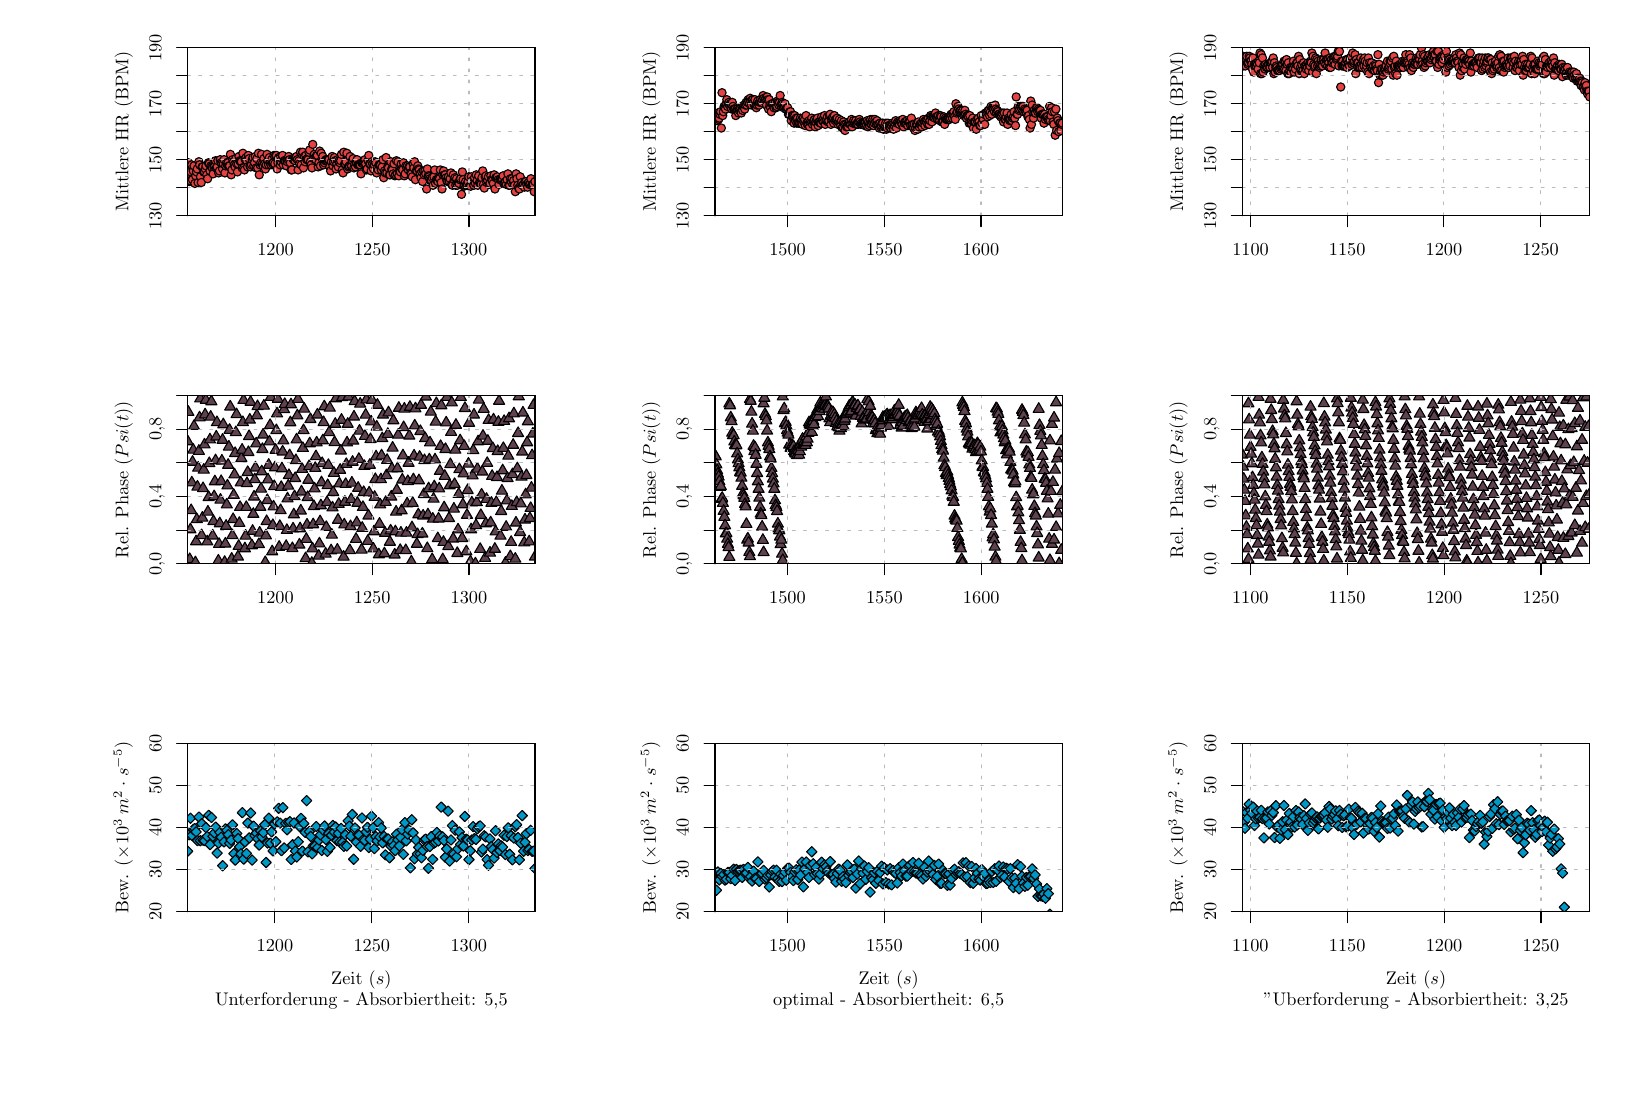
\begin{tikzpicture}[x=1pt,y=1pt]
\definecolor{fillColor}{RGB}{255,255,255}
\path[use as bounding box,fill=fillColor,fill opacity=0.00] (0,0) rectangle (571.66,377.25);
\begin{scope}
\path[clip] ( 57.82,309.32) rectangle (183.32,370.02);
\definecolor{drawColor}{RGB}{0,0,0}
\definecolor{fillColor}{RGB}{229,66,66}

\path[draw=drawColor,line width= 0.4pt,line join=round,line cap=round,fill=fillColor] ( 57.82,324.42) circle (  1.49);

\path[draw=drawColor,line width= 0.4pt,line join=round,line cap=round,fill=fillColor] ( 58.10,328.42) circle (  1.49);

\path[draw=drawColor,line width= 0.4pt,line join=round,line cap=round,fill=fillColor] ( 58.39,321.64) circle (  1.49);

\path[draw=drawColor,line width= 0.4pt,line join=round,line cap=round,fill=fillColor] ( 58.69,321.98) circle (  1.49);

\path[draw=drawColor,line width= 0.4pt,line join=round,line cap=round,fill=fillColor] ( 58.97,325.13) circle (  1.49);

\path[draw=drawColor,line width= 0.4pt,line join=round,line cap=round,fill=fillColor] ( 59.26,327.68) circle (  1.49);

\path[draw=drawColor,line width= 0.4pt,line join=round,line cap=round,fill=fillColor] ( 59.55,322.32) circle (  1.49);

\path[draw=drawColor,line width= 0.4pt,line join=round,line cap=round,fill=fillColor] ( 59.84,325.49) circle (  1.49);

\path[draw=drawColor,line width= 0.4pt,line join=round,line cap=round,fill=fillColor] ( 60.12,327.31) circle (  1.49);

\path[draw=drawColor,line width= 0.4pt,line join=round,line cap=round,fill=fillColor] ( 60.42,320.96) circle (  1.49);

\path[draw=drawColor,line width= 0.4pt,line join=round,line cap=round,fill=fillColor] ( 60.71,323.71) circle (  1.49);

\path[draw=drawColor,line width= 0.4pt,line join=round,line cap=round,fill=fillColor] ( 61.00,325.13) circle (  1.49);

\path[draw=drawColor,line width= 0.4pt,line join=round,line cap=round,fill=fillColor] ( 61.28,326.21) circle (  1.49);

\path[draw=drawColor,line width= 0.4pt,line join=round,line cap=round,fill=fillColor] ( 61.58,321.30) circle (  1.49);

\path[draw=drawColor,line width= 0.4pt,line join=round,line cap=round,fill=fillColor] ( 61.86,328.80) circle (  1.49);

\path[draw=drawColor,line width= 0.4pt,line join=round,line cap=round,fill=fillColor] ( 62.14,327.68) circle (  1.49);

\path[draw=drawColor,line width= 0.4pt,line join=round,line cap=round,fill=fillColor] ( 62.43,323.36) circle (  1.49);

\path[draw=drawColor,line width= 0.4pt,line join=round,line cap=round,fill=fillColor] ( 62.73,321.30) circle (  1.49);

\path[draw=drawColor,line width= 0.4pt,line join=round,line cap=round,fill=fillColor] ( 63.01,326.94) circle (  1.49);

\path[draw=drawColor,line width= 0.4pt,line join=round,line cap=round,fill=fillColor] ( 63.30,326.94) circle (  1.49);

\path[draw=drawColor,line width= 0.4pt,line join=round,line cap=round,fill=fillColor] ( 63.59,325.13) circle (  1.49);

\path[draw=drawColor,line width= 0.4pt,line join=round,line cap=round,fill=fillColor] ( 63.87,325.13) circle (  1.49);

\path[draw=drawColor,line width= 0.4pt,line join=round,line cap=round,fill=fillColor] ( 64.16,326.21) circle (  1.49);

\path[draw=drawColor,line width= 0.4pt,line join=round,line cap=round,fill=fillColor] ( 64.44,327.31) circle (  1.49);

\path[draw=drawColor,line width= 0.4pt,line join=round,line cap=round,fill=fillColor] ( 64.73,324.07) circle (  1.49);

\path[draw=drawColor,line width= 0.4pt,line join=round,line cap=round,fill=fillColor] ( 65.03,322.67) circle (  1.49);

\path[draw=drawColor,line width= 0.4pt,line join=round,line cap=round,fill=fillColor] ( 65.31,328.42) circle (  1.49);

\path[draw=drawColor,line width= 0.4pt,line join=round,line cap=round,fill=fillColor] ( 65.59,328.05) circle (  1.49);

\path[draw=drawColor,line width= 0.4pt,line join=round,line cap=round,fill=fillColor] ( 65.88,325.49) circle (  1.49);

\path[draw=drawColor,line width= 0.4pt,line join=round,line cap=round,fill=fillColor] ( 66.16,327.31) circle (  1.49);

\path[draw=drawColor,line width= 0.4pt,line join=round,line cap=round,fill=fillColor] ( 66.45,326.94) circle (  1.49);

\path[draw=drawColor,line width= 0.4pt,line join=round,line cap=round,fill=fillColor] ( 66.73,326.58) circle (  1.49);

\path[draw=drawColor,line width= 0.4pt,line join=round,line cap=round,fill=fillColor] ( 67.02,324.42) circle (  1.49);

\path[draw=drawColor,line width= 0.4pt,line join=round,line cap=round,fill=fillColor] ( 67.30,326.94) circle (  1.49);

\path[draw=drawColor,line width= 0.4pt,line join=round,line cap=round,fill=fillColor] ( 67.59,327.31) circle (  1.49);

\path[draw=drawColor,line width= 0.4pt,line join=round,line cap=round,fill=fillColor] ( 67.87,329.17) circle (  1.49);

\path[draw=drawColor,line width= 0.4pt,line join=round,line cap=round,fill=fillColor] ( 68.15,326.58) circle (  1.49);

\path[draw=drawColor,line width= 0.4pt,line join=round,line cap=round,fill=fillColor] ( 68.44,326.94) circle (  1.49);

\path[draw=drawColor,line width= 0.4pt,line join=round,line cap=round,fill=fillColor] ( 68.72,329.17) circle (  1.49);

\path[draw=drawColor,line width= 0.4pt,line join=round,line cap=round,fill=fillColor] ( 69.01,324.77) circle (  1.49);

\path[draw=drawColor,line width= 0.4pt,line join=round,line cap=round,fill=fillColor] ( 69.29,325.49) circle (  1.49);

\path[draw=drawColor,line width= 0.4pt,line join=round,line cap=round,fill=fillColor] ( 69.57,329.55) circle (  1.49);

\path[draw=drawColor,line width= 0.4pt,line join=round,line cap=round,fill=fillColor] ( 69.86,328.42) circle (  1.49);

\path[draw=drawColor,line width= 0.4pt,line join=round,line cap=round,fill=fillColor] ( 70.14,328.05) circle (  1.49);

\path[draw=drawColor,line width= 0.4pt,line join=round,line cap=round,fill=fillColor] ( 70.42,326.21) circle (  1.49);

\path[draw=drawColor,line width= 0.4pt,line join=round,line cap=round,fill=fillColor] ( 70.71,328.05) circle (  1.49);

\path[draw=drawColor,line width= 0.4pt,line join=round,line cap=round,fill=fillColor] ( 70.99,329.55) circle (  1.49);

\path[draw=drawColor,line width= 0.4pt,line join=round,line cap=round,fill=fillColor] ( 71.27,324.77) circle (  1.49);

\path[draw=drawColor,line width= 0.4pt,line join=round,line cap=round,fill=fillColor] ( 71.56,327.31) circle (  1.49);

\path[draw=drawColor,line width= 0.4pt,line join=round,line cap=round,fill=fillColor] ( 71.84,328.42) circle (  1.49);

\path[draw=drawColor,line width= 0.4pt,line join=round,line cap=round,fill=fillColor] ( 72.12,327.68) circle (  1.49);

\path[draw=drawColor,line width= 0.4pt,line join=round,line cap=round,fill=fillColor] ( 72.40,328.42) circle (  1.49);

\path[draw=drawColor,line width= 0.4pt,line join=round,line cap=round,fill=fillColor] ( 72.69,327.31) circle (  1.49);

\path[draw=drawColor,line width= 0.4pt,line join=round,line cap=round,fill=fillColor] ( 72.97,327.31) circle (  1.49);

\path[draw=drawColor,line width= 0.4pt,line join=round,line cap=round,fill=fillColor] ( 73.25,331.47) circle (  1.49);

\path[draw=drawColor,line width= 0.4pt,line join=round,line cap=round,fill=fillColor] ( 73.54,324.07) circle (  1.49);

\path[draw=drawColor,line width= 0.4pt,line join=round,line cap=round,fill=fillColor] ( 73.82,325.85) circle (  1.49);

\path[draw=drawColor,line width= 0.4pt,line join=round,line cap=round,fill=fillColor] ( 74.10,329.55) circle (  1.49);

\path[draw=drawColor,line width= 0.4pt,line join=round,line cap=round,fill=fillColor] ( 74.38,328.80) circle (  1.49);

\path[draw=drawColor,line width= 0.4pt,line join=round,line cap=round,fill=fillColor] ( 74.67,327.68) circle (  1.49);

\path[draw=drawColor,line width= 0.4pt,line join=round,line cap=round,fill=fillColor] ( 74.95,326.94) circle (  1.49);

\path[draw=drawColor,line width= 0.4pt,line join=round,line cap=round,fill=fillColor] ( 75.23,329.93) circle (  1.49);

\path[draw=drawColor,line width= 0.4pt,line join=round,line cap=round,fill=fillColor] ( 75.51,328.05) circle (  1.49);

\path[draw=drawColor,line width= 0.4pt,line join=round,line cap=round,fill=fillColor] ( 75.80,325.13) circle (  1.49);

\path[draw=drawColor,line width= 0.4pt,line join=round,line cap=round,fill=fillColor] ( 76.08,328.05) circle (  1.49);

\path[draw=drawColor,line width= 0.4pt,line join=round,line cap=round,fill=fillColor] ( 76.36,330.70) circle (  1.49);

\path[draw=drawColor,line width= 0.4pt,line join=round,line cap=round,fill=fillColor] ( 76.64,329.17) circle (  1.49);

\path[draw=drawColor,line width= 0.4pt,line join=round,line cap=round,fill=fillColor] ( 76.92,328.80) circle (  1.49);

\path[draw=drawColor,line width= 0.4pt,line join=round,line cap=round,fill=fillColor] ( 77.20,328.80) circle (  1.49);

\path[draw=drawColor,line width= 0.4pt,line join=round,line cap=round,fill=fillColor] ( 77.49,326.58) circle (  1.49);

\path[draw=drawColor,line width= 0.4pt,line join=round,line cap=round,fill=fillColor] ( 77.76,331.86) circle (  1.49);

\path[draw=drawColor,line width= 0.4pt,line join=round,line cap=round,fill=fillColor] ( 78.05,326.58) circle (  1.49);

\path[draw=drawColor,line width= 0.4pt,line join=round,line cap=round,fill=fillColor] ( 78.33,325.85) circle (  1.49);

\path[draw=drawColor,line width= 0.4pt,line join=round,line cap=round,fill=fillColor] ( 78.61,329.55) circle (  1.49);

\path[draw=drawColor,line width= 0.4pt,line join=round,line cap=round,fill=fillColor] ( 78.89,330.31) circle (  1.49);

\path[draw=drawColor,line width= 0.4pt,line join=round,line cap=round,fill=fillColor] ( 79.17,329.17) circle (  1.49);

\path[draw=drawColor,line width= 0.4pt,line join=round,line cap=round,fill=fillColor] ( 79.46,326.94) circle (  1.49);

\path[draw=drawColor,line width= 0.4pt,line join=round,line cap=round,fill=fillColor] ( 79.73,331.08) circle (  1.49);

\path[draw=drawColor,line width= 0.4pt,line join=round,line cap=round,fill=fillColor] ( 80.01,329.93) circle (  1.49);

\path[draw=drawColor,line width= 0.4pt,line join=round,line cap=round,fill=fillColor] ( 80.30,327.31) circle (  1.49);

\path[draw=drawColor,line width= 0.4pt,line join=round,line cap=round,fill=fillColor] ( 80.58,326.94) circle (  1.49);

\path[draw=drawColor,line width= 0.4pt,line join=round,line cap=round,fill=fillColor] ( 80.86,327.68) circle (  1.49);

\path[draw=drawColor,line width= 0.4pt,line join=round,line cap=round,fill=fillColor] ( 81.14,329.55) circle (  1.49);

\path[draw=drawColor,line width= 0.4pt,line join=round,line cap=round,fill=fillColor] ( 81.42,330.31) circle (  1.49);

\path[draw=drawColor,line width= 0.4pt,line join=round,line cap=round,fill=fillColor] ( 81.71,327.31) circle (  1.49);

\path[draw=drawColor,line width= 0.4pt,line join=round,line cap=round,fill=fillColor] ( 81.99,328.42) circle (  1.49);

\path[draw=drawColor,line width= 0.4pt,line join=round,line cap=round,fill=fillColor] ( 82.26,330.70) circle (  1.49);

\path[draw=drawColor,line width= 0.4pt,line join=round,line cap=round,fill=fillColor] ( 82.55,326.58) circle (  1.49);

\path[draw=drawColor,line width= 0.4pt,line join=round,line cap=round,fill=fillColor] ( 82.83,329.93) circle (  1.49);

\path[draw=drawColor,line width= 0.4pt,line join=round,line cap=round,fill=fillColor] ( 83.11,326.58) circle (  1.49);

\path[draw=drawColor,line width= 0.4pt,line join=round,line cap=round,fill=fillColor] ( 83.39,331.86) circle (  1.49);

\path[draw=drawColor,line width= 0.4pt,line join=round,line cap=round,fill=fillColor] ( 83.68,324.07) circle (  1.49);

\path[draw=drawColor,line width= 0.4pt,line join=round,line cap=round,fill=fillColor] ( 83.96,327.68) circle (  1.49);

\path[draw=drawColor,line width= 0.4pt,line join=round,line cap=round,fill=fillColor] ( 84.24,328.42) circle (  1.49);

\path[draw=drawColor,line width= 0.4pt,line join=round,line cap=round,fill=fillColor] ( 84.52,331.47) circle (  1.49);

\path[draw=drawColor,line width= 0.4pt,line join=round,line cap=round,fill=fillColor] ( 84.80,328.05) circle (  1.49);

\path[draw=drawColor,line width= 0.4pt,line join=round,line cap=round,fill=fillColor] ( 85.09,327.31) circle (  1.49);

\path[draw=drawColor,line width= 0.4pt,line join=round,line cap=round,fill=fillColor] ( 85.36,329.93) circle (  1.49);

\path[draw=drawColor,line width= 0.4pt,line join=round,line cap=round,fill=fillColor] ( 85.65,328.05) circle (  1.49);

\path[draw=drawColor,line width= 0.4pt,line join=round,line cap=round,fill=fillColor] ( 85.93,326.21) circle (  1.49);

\path[draw=drawColor,line width= 0.4pt,line join=round,line cap=round,fill=fillColor] ( 86.22,327.68) circle (  1.49);

\path[draw=drawColor,line width= 0.4pt,line join=round,line cap=round,fill=fillColor] ( 86.49,331.47) circle (  1.49);

\path[draw=drawColor,line width= 0.4pt,line join=round,line cap=round,fill=fillColor] ( 86.77,329.17) circle (  1.49);

\path[draw=drawColor,line width= 0.4pt,line join=round,line cap=round,fill=fillColor] ( 87.05,327.68) circle (  1.49);

\path[draw=drawColor,line width= 0.4pt,line join=round,line cap=round,fill=fillColor] ( 87.33,330.31) circle (  1.49);

\path[draw=drawColor,line width= 0.4pt,line join=round,line cap=round,fill=fillColor] ( 87.61,328.42) circle (  1.49);

\path[draw=drawColor,line width= 0.4pt,line join=round,line cap=round,fill=fillColor] ( 87.90,327.68) circle (  1.49);

\path[draw=drawColor,line width= 0.4pt,line join=round,line cap=round,fill=fillColor] ( 88.18,329.55) circle (  1.49);

\path[draw=drawColor,line width= 0.4pt,line join=round,line cap=round,fill=fillColor] ( 88.46,328.05) circle (  1.49);

\path[draw=drawColor,line width= 0.4pt,line join=round,line cap=round,fill=fillColor] ( 88.74,328.42) circle (  1.49);

\path[draw=drawColor,line width= 0.4pt,line join=round,line cap=round,fill=fillColor] ( 89.02,331.08) circle (  1.49);

\path[draw=drawColor,line width= 0.4pt,line join=round,line cap=round,fill=fillColor] ( 89.30,328.05) circle (  1.49);

\path[draw=drawColor,line width= 0.4pt,line join=round,line cap=round,fill=fillColor] ( 89.58,331.08) circle (  1.49);

\path[draw=drawColor,line width= 0.4pt,line join=round,line cap=round,fill=fillColor] ( 89.85,331.08) circle (  1.49);

\path[draw=drawColor,line width= 0.4pt,line join=round,line cap=round,fill=fillColor] ( 90.14,326.21) circle (  1.49);

\path[draw=drawColor,line width= 0.4pt,line join=round,line cap=round,fill=fillColor] ( 90.42,328.42) circle (  1.49);

\path[draw=drawColor,line width= 0.4pt,line join=round,line cap=round,fill=fillColor] ( 90.70,330.31) circle (  1.49);

\path[draw=drawColor,line width= 0.4pt,line join=round,line cap=round,fill=fillColor] ( 90.98,329.93) circle (  1.49);

\path[draw=drawColor,line width= 0.4pt,line join=round,line cap=round,fill=fillColor] ( 91.26,327.68) circle (  1.49);

\path[draw=drawColor,line width= 0.4pt,line join=round,line cap=round,fill=fillColor] ( 91.54,328.80) circle (  1.49);

\path[draw=drawColor,line width= 0.4pt,line join=round,line cap=round,fill=fillColor] ( 91.82,329.93) circle (  1.49);

\path[draw=drawColor,line width= 0.4pt,line join=round,line cap=round,fill=fillColor] ( 92.10,331.08) circle (  1.49);

\path[draw=drawColor,line width= 0.4pt,line join=round,line cap=round,fill=fillColor] ( 92.38,327.68) circle (  1.49);

\path[draw=drawColor,line width= 0.4pt,line join=round,line cap=round,fill=fillColor] ( 92.66,329.17) circle (  1.49);

\path[draw=drawColor,line width= 0.4pt,line join=round,line cap=round,fill=fillColor] ( 92.94,329.17) circle (  1.49);

\path[draw=drawColor,line width= 0.4pt,line join=round,line cap=round,fill=fillColor] ( 93.22,328.80) circle (  1.49);

\path[draw=drawColor,line width= 0.4pt,line join=round,line cap=round,fill=fillColor] ( 93.51,327.31) circle (  1.49);

\path[draw=drawColor,line width= 0.4pt,line join=round,line cap=round,fill=fillColor] ( 93.79,328.80) circle (  1.49);

\path[draw=drawColor,line width= 0.4pt,line join=round,line cap=round,fill=fillColor] ( 94.07,329.55) circle (  1.49);

\path[draw=drawColor,line width= 0.4pt,line join=round,line cap=round,fill=fillColor] ( 94.34,330.70) circle (  1.49);

\path[draw=drawColor,line width= 0.4pt,line join=round,line cap=round,fill=fillColor] ( 94.62,329.55) circle (  1.49);

\path[draw=drawColor,line width= 0.4pt,line join=round,line cap=round,fill=fillColor] ( 94.90,328.42) circle (  1.49);

\path[draw=drawColor,line width= 0.4pt,line join=round,line cap=round,fill=fillColor] ( 95.19,325.85) circle (  1.49);

\path[draw=drawColor,line width= 0.4pt,line join=round,line cap=round,fill=fillColor] ( 95.48,325.85) circle (  1.49);

\path[draw=drawColor,line width= 0.4pt,line join=round,line cap=round,fill=fillColor] ( 95.76,329.93) circle (  1.49);

\path[draw=drawColor,line width= 0.4pt,line join=round,line cap=round,fill=fillColor] ( 96.04,329.55) circle (  1.49);

\path[draw=drawColor,line width= 0.4pt,line join=round,line cap=round,fill=fillColor] ( 96.32,329.55) circle (  1.49);

\path[draw=drawColor,line width= 0.4pt,line join=round,line cap=round,fill=fillColor] ( 96.60,329.17) circle (  1.49);

\path[draw=drawColor,line width= 0.4pt,line join=round,line cap=round,fill=fillColor] ( 96.87,330.31) circle (  1.49);

\path[draw=drawColor,line width= 0.4pt,line join=round,line cap=round,fill=fillColor] ( 97.15,330.70) circle (  1.49);

\path[draw=drawColor,line width= 0.4pt,line join=round,line cap=round,fill=fillColor] ( 97.43,329.55) circle (  1.49);

\path[draw=drawColor,line width= 0.4pt,line join=round,line cap=round,fill=fillColor] ( 97.72,325.85) circle (  1.49);

\path[draw=drawColor,line width= 0.4pt,line join=round,line cap=round,fill=fillColor] ( 98.00,329.17) circle (  1.49);

\path[draw=drawColor,line width= 0.4pt,line join=round,line cap=round,fill=fillColor] ( 98.28,328.05) circle (  1.49);

\path[draw=drawColor,line width= 0.4pt,line join=round,line cap=round,fill=fillColor] ( 98.55,332.25) circle (  1.49);

\path[draw=drawColor,line width= 0.4pt,line join=round,line cap=round,fill=fillColor] ( 98.84,327.68) circle (  1.49);

\path[draw=drawColor,line width= 0.4pt,line join=round,line cap=round,fill=fillColor] ( 99.11,331.47) circle (  1.49);

\path[draw=drawColor,line width= 0.4pt,line join=round,line cap=round,fill=fillColor] ( 99.39,332.25) circle (  1.49);

\path[draw=drawColor,line width= 0.4pt,line join=round,line cap=round,fill=fillColor] ( 99.67,326.58) circle (  1.49);

\path[draw=drawColor,line width= 0.4pt,line join=round,line cap=round,fill=fillColor] ( 99.95,330.70) circle (  1.49);

\path[draw=drawColor,line width= 0.4pt,line join=round,line cap=round,fill=fillColor] (100.23,328.80) circle (  1.49);

\path[draw=drawColor,line width= 0.4pt,line join=round,line cap=round,fill=fillColor] (100.51,331.08) circle (  1.49);

\path[draw=drawColor,line width= 0.4pt,line join=round,line cap=round,fill=fillColor] (100.79,329.55) circle (  1.49);

\path[draw=drawColor,line width= 0.4pt,line join=round,line cap=round,fill=fillColor] (101.07,329.93) circle (  1.49);

\path[draw=drawColor,line width= 0.4pt,line join=round,line cap=round,fill=fillColor] (101.35,329.55) circle (  1.49);

\path[draw=drawColor,line width= 0.4pt,line join=round,line cap=round,fill=fillColor] (101.62,332.25) circle (  1.49);

\path[draw=drawColor,line width= 0.4pt,line join=round,line cap=round,fill=fillColor] (101.89,333.04) circle (  1.49);

\path[draw=drawColor,line width= 0.4pt,line join=round,line cap=round,fill=fillColor] (102.17,328.80) circle (  1.49);

\path[draw=drawColor,line width= 0.4pt,line join=round,line cap=round,fill=fillColor] (102.46,327.68) circle (  1.49);

\path[draw=drawColor,line width= 0.4pt,line join=round,line cap=round,fill=fillColor] (102.74,326.58) circle (  1.49);

\path[draw=drawColor,line width= 0.4pt,line join=round,line cap=round,fill=fillColor] (103.01,335.06) circle (  1.49);

\path[draw=drawColor,line width= 0.4pt,line join=round,line cap=round,fill=fillColor] (103.29,329.93) circle (  1.49);

\path[draw=drawColor,line width= 0.4pt,line join=round,line cap=round,fill=fillColor] (103.57,331.47) circle (  1.49);

\path[draw=drawColor,line width= 0.4pt,line join=round,line cap=round,fill=fillColor] (103.85,330.31) circle (  1.49);

\path[draw=drawColor,line width= 0.4pt,line join=round,line cap=round,fill=fillColor] (104.13,329.55) circle (  1.49);

\path[draw=drawColor,line width= 0.4pt,line join=round,line cap=round,fill=fillColor] (104.40,331.08) circle (  1.49);

\path[draw=drawColor,line width= 0.4pt,line join=round,line cap=round,fill=fillColor] (104.68,331.08) circle (  1.49);

\path[draw=drawColor,line width= 0.4pt,line join=round,line cap=round,fill=fillColor] (104.96,326.94) circle (  1.49);

\path[draw=drawColor,line width= 0.4pt,line join=round,line cap=round,fill=fillColor] (105.24,328.42) circle (  1.49);

\path[draw=drawColor,line width= 0.4pt,line join=round,line cap=round,fill=fillColor] (105.52,332.65) circle (  1.49);

\path[draw=drawColor,line width= 0.4pt,line join=round,line cap=round,fill=fillColor] (105.80,327.31) circle (  1.49);

\path[draw=drawColor,line width= 0.4pt,line join=round,line cap=round,fill=fillColor] (106.08,331.86) circle (  1.49);

\path[draw=drawColor,line width= 0.4pt,line join=round,line cap=round,fill=fillColor] (106.36,329.93) circle (  1.49);

\path[draw=drawColor,line width= 0.4pt,line join=round,line cap=round,fill=fillColor] (106.63,330.70) circle (  1.49);

\path[draw=drawColor,line width= 0.4pt,line join=round,line cap=round,fill=fillColor] (106.92,327.68) circle (  1.49);

\path[draw=drawColor,line width= 0.4pt,line join=round,line cap=round,fill=fillColor] (107.20,328.42) circle (  1.49);

\path[draw=drawColor,line width= 0.4pt,line join=round,line cap=round,fill=fillColor] (107.48,329.17) circle (  1.49);

\path[draw=drawColor,line width= 0.4pt,line join=round,line cap=round,fill=fillColor] (107.76,329.55) circle (  1.49);

\path[draw=drawColor,line width= 0.4pt,line join=round,line cap=round,fill=fillColor] (108.04,329.55) circle (  1.49);

\path[draw=drawColor,line width= 0.4pt,line join=round,line cap=round,fill=fillColor] (108.32,329.17) circle (  1.49);

\path[draw=drawColor,line width= 0.4pt,line join=round,line cap=round,fill=fillColor] (108.60,329.55) circle (  1.49);

\path[draw=drawColor,line width= 0.4pt,line join=round,line cap=round,fill=fillColor] (108.88,329.55) circle (  1.49);

\path[draw=drawColor,line width= 0.4pt,line join=round,line cap=round,fill=fillColor] (109.16,326.94) circle (  1.49);

\path[draw=drawColor,line width= 0.4pt,line join=round,line cap=round,fill=fillColor] (109.45,325.49) circle (  1.49);

\path[draw=drawColor,line width= 0.4pt,line join=round,line cap=round,fill=fillColor] (109.73,328.80) circle (  1.49);

\path[draw=drawColor,line width= 0.4pt,line join=round,line cap=round,fill=fillColor] (110.01,330.70) circle (  1.49);

\path[draw=drawColor,line width= 0.4pt,line join=round,line cap=round,fill=fillColor] (110.29,327.31) circle (  1.49);

\path[draw=drawColor,line width= 0.4pt,line join=round,line cap=round,fill=fillColor] (110.57,328.80) circle (  1.49);

\path[draw=drawColor,line width= 0.4pt,line join=round,line cap=round,fill=fillColor] (110.85,330.31) circle (  1.49);

\path[draw=drawColor,line width= 0.4pt,line join=round,line cap=round,fill=fillColor] (111.13,329.17) circle (  1.49);

\path[draw=drawColor,line width= 0.4pt,line join=round,line cap=round,fill=fillColor] (111.42,326.21) circle (  1.49);

\path[draw=drawColor,line width= 0.4pt,line join=round,line cap=round,fill=fillColor] (111.70,328.05) circle (  1.49);

\path[draw=drawColor,line width= 0.4pt,line join=round,line cap=round,fill=fillColor] (111.98,329.55) circle (  1.49);

\path[draw=drawColor,line width= 0.4pt,line join=round,line cap=round,fill=fillColor] (112.26,326.94) circle (  1.49);

\path[draw=drawColor,line width= 0.4pt,line join=round,line cap=round,fill=fillColor] (112.54,329.17) circle (  1.49);

\path[draw=drawColor,line width= 0.4pt,line join=round,line cap=round,fill=fillColor] (112.82,328.42) circle (  1.49);

\path[draw=drawColor,line width= 0.4pt,line join=round,line cap=round,fill=fillColor] (113.10,329.17) circle (  1.49);

\path[draw=drawColor,line width= 0.4pt,line join=round,line cap=round,fill=fillColor] (113.38,331.47) circle (  1.49);

\path[draw=drawColor,line width= 0.4pt,line join=round,line cap=round,fill=fillColor] (113.67,325.85) circle (  1.49);

\path[draw=drawColor,line width= 0.4pt,line join=round,line cap=round,fill=fillColor] (113.96,324.77) circle (  1.49);

\path[draw=drawColor,line width= 0.4pt,line join=round,line cap=round,fill=fillColor] (114.23,332.25) circle (  1.49);

\path[draw=drawColor,line width= 0.4pt,line join=round,line cap=round,fill=fillColor] (114.51,328.05) circle (  1.49);

\path[draw=drawColor,line width= 0.4pt,line join=round,line cap=round,fill=fillColor] (114.79,328.05) circle (  1.49);

\path[draw=drawColor,line width= 0.4pt,line join=round,line cap=round,fill=fillColor] (115.08,328.80) circle (  1.49);

\path[draw=drawColor,line width= 0.4pt,line join=round,line cap=round,fill=fillColor] (115.35,331.86) circle (  1.49);

\path[draw=drawColor,line width= 0.4pt,line join=round,line cap=round,fill=fillColor] (115.64,326.21) circle (  1.49);

\path[draw=drawColor,line width= 0.4pt,line join=round,line cap=round,fill=fillColor] (115.92,326.94) circle (  1.49);

\path[draw=drawColor,line width= 0.4pt,line join=round,line cap=round,fill=fillColor] (116.20,327.31) circle (  1.49);

\path[draw=drawColor,line width= 0.4pt,line join=round,line cap=round,fill=fillColor] (116.48,330.70) circle (  1.49);

\path[draw=drawColor,line width= 0.4pt,line join=round,line cap=round,fill=fillColor] (116.77,327.68) circle (  1.49);

\path[draw=drawColor,line width= 0.4pt,line join=round,line cap=round,fill=fillColor] (117.05,327.31) circle (  1.49);

\path[draw=drawColor,line width= 0.4pt,line join=round,line cap=round,fill=fillColor] (117.33,329.17) circle (  1.49);

\path[draw=drawColor,line width= 0.4pt,line join=round,line cap=round,fill=fillColor] (117.61,329.93) circle (  1.49);

\path[draw=drawColor,line width= 0.4pt,line join=round,line cap=round,fill=fillColor] (117.89,326.58) circle (  1.49);

\path[draw=drawColor,line width= 0.4pt,line join=round,line cap=round,fill=fillColor] (118.18,328.05) circle (  1.49);

\path[draw=drawColor,line width= 0.4pt,line join=round,line cap=round,fill=fillColor] (118.46,326.94) circle (  1.49);

\path[draw=drawColor,line width= 0.4pt,line join=round,line cap=round,fill=fillColor] (118.74,328.42) circle (  1.49);

\path[draw=drawColor,line width= 0.4pt,line join=round,line cap=round,fill=fillColor] (119.02,329.55) circle (  1.49);

\path[draw=drawColor,line width= 0.4pt,line join=round,line cap=round,fill=fillColor] (119.30,327.68) circle (  1.49);

\path[draw=drawColor,line width= 0.4pt,line join=round,line cap=round,fill=fillColor] (119.59,327.68) circle (  1.49);

\path[draw=drawColor,line width= 0.4pt,line join=round,line cap=round,fill=fillColor] (119.87,327.68) circle (  1.49);

\path[draw=drawColor,line width= 0.4pt,line join=round,line cap=round,fill=fillColor] (120.15,327.68) circle (  1.49);

\path[draw=drawColor,line width= 0.4pt,line join=round,line cap=round,fill=fillColor] (120.44,324.42) circle (  1.49);

\path[draw=drawColor,line width= 0.4pt,line join=round,line cap=round,fill=fillColor] (120.72,328.42) circle (  1.49);

\path[draw=drawColor,line width= 0.4pt,line join=round,line cap=round,fill=fillColor] (121.01,328.42) circle (  1.49);

\path[draw=drawColor,line width= 0.4pt,line join=round,line cap=round,fill=fillColor] (121.29,328.05) circle (  1.49);

\path[draw=drawColor,line width= 0.4pt,line join=round,line cap=round,fill=fillColor] (121.57,328.42) circle (  1.49);

\path[draw=drawColor,line width= 0.4pt,line join=round,line cap=round,fill=fillColor] (121.85,329.55) circle (  1.49);

\path[draw=drawColor,line width= 0.4pt,line join=round,line cap=round,fill=fillColor] (122.13,328.05) circle (  1.49);

\path[draw=drawColor,line width= 0.4pt,line join=round,line cap=round,fill=fillColor] (122.42,325.85) circle (  1.49);

\path[draw=drawColor,line width= 0.4pt,line join=round,line cap=round,fill=fillColor] (122.70,326.21) circle (  1.49);

\path[draw=drawColor,line width= 0.4pt,line join=round,line cap=round,fill=fillColor] (122.98,329.17) circle (  1.49);

\path[draw=drawColor,line width= 0.4pt,line join=round,line cap=round,fill=fillColor] (123.26,331.08) circle (  1.49);

\path[draw=drawColor,line width= 0.4pt,line join=round,line cap=round,fill=fillColor] (123.54,328.05) circle (  1.49);

\path[draw=drawColor,line width= 0.4pt,line join=round,line cap=round,fill=fillColor] (123.83,328.05) circle (  1.49);

\path[draw=drawColor,line width= 0.4pt,line join=round,line cap=round,fill=fillColor] (124.11,325.49) circle (  1.49);

\path[draw=drawColor,line width= 0.4pt,line join=round,line cap=round,fill=fillColor] (124.39,328.80) circle (  1.49);

\path[draw=drawColor,line width= 0.4pt,line join=round,line cap=round,fill=fillColor] (124.68,328.05) circle (  1.49);

\path[draw=drawColor,line width= 0.4pt,line join=round,line cap=round,fill=fillColor] (124.96,326.21) circle (  1.49);

\path[draw=drawColor,line width= 0.4pt,line join=round,line cap=round,fill=fillColor] (125.24,327.68) circle (  1.49);

\path[draw=drawColor,line width= 0.4pt,line join=round,line cap=round,fill=fillColor] (125.53,328.80) circle (  1.49);

\path[draw=drawColor,line width= 0.4pt,line join=round,line cap=round,fill=fillColor] (125.81,328.42) circle (  1.49);

\path[draw=drawColor,line width= 0.4pt,line join=round,line cap=round,fill=fillColor] (126.10,324.77) circle (  1.49);

\path[draw=drawColor,line width= 0.4pt,line join=round,line cap=round,fill=fillColor] (126.38,326.58) circle (  1.49);

\path[draw=drawColor,line width= 0.4pt,line join=round,line cap=round,fill=fillColor] (126.67,325.85) circle (  1.49);

\path[draw=drawColor,line width= 0.4pt,line join=round,line cap=round,fill=fillColor] (126.95,327.68) circle (  1.49);

\path[draw=drawColor,line width= 0.4pt,line join=round,line cap=round,fill=fillColor] (127.23,327.68) circle (  1.49);

\path[draw=drawColor,line width= 0.4pt,line join=round,line cap=round,fill=fillColor] (127.52,327.68) circle (  1.49);

\path[draw=drawColor,line width= 0.4pt,line join=round,line cap=round,fill=fillColor] (127.80,325.85) circle (  1.49);

\path[draw=drawColor,line width= 0.4pt,line join=round,line cap=round,fill=fillColor] (128.09,326.94) circle (  1.49);

\path[draw=drawColor,line width= 0.4pt,line join=round,line cap=round,fill=fillColor] (128.37,329.55) circle (  1.49);

\path[draw=drawColor,line width= 0.4pt,line join=round,line cap=round,fill=fillColor] (128.66,323.02) circle (  1.49);

\path[draw=drawColor,line width= 0.4pt,line join=round,line cap=round,fill=fillColor] (128.95,325.49) circle (  1.49);

\path[draw=drawColor,line width= 0.4pt,line join=round,line cap=round,fill=fillColor] (129.24,324.77) circle (  1.49);

\path[draw=drawColor,line width= 0.4pt,line join=round,line cap=round,fill=fillColor] (129.51,330.31) circle (  1.49);

\path[draw=drawColor,line width= 0.4pt,line join=round,line cap=round,fill=fillColor] (129.80,324.77) circle (  1.49);

\path[draw=drawColor,line width= 0.4pt,line join=round,line cap=round,fill=fillColor] (130.09,326.94) circle (  1.49);

\path[draw=drawColor,line width= 0.4pt,line join=round,line cap=round,fill=fillColor] (130.37,326.58) circle (  1.49);

\path[draw=drawColor,line width= 0.4pt,line join=round,line cap=round,fill=fillColor] (130.66,324.07) circle (  1.49);

\path[draw=drawColor,line width= 0.4pt,line join=round,line cap=round,fill=fillColor] (130.95,324.07) circle (  1.49);

\path[draw=drawColor,line width= 0.4pt,line join=round,line cap=round,fill=fillColor] (131.23,328.80) circle (  1.49);

\path[draw=drawColor,line width= 0.4pt,line join=round,line cap=round,fill=fillColor] (131.52,326.21) circle (  1.49);

\path[draw=drawColor,line width= 0.4pt,line join=round,line cap=round,fill=fillColor] (131.80,325.85) circle (  1.49);

\path[draw=drawColor,line width= 0.4pt,line join=round,line cap=round,fill=fillColor] (132.09,324.42) circle (  1.49);

\path[draw=drawColor,line width= 0.4pt,line join=round,line cap=round,fill=fillColor] (132.38,328.05) circle (  1.49);

\path[draw=drawColor,line width= 0.4pt,line join=round,line cap=round,fill=fillColor] (132.67,323.71) circle (  1.49);

\path[draw=drawColor,line width= 0.4pt,line join=round,line cap=round,fill=fillColor] (132.96,324.07) circle (  1.49);

\path[draw=drawColor,line width= 0.4pt,line join=round,line cap=round,fill=fillColor] (133.24,329.17) circle (  1.49);

\path[draw=drawColor,line width= 0.4pt,line join=round,line cap=round,fill=fillColor] (133.53,324.42) circle (  1.49);

\path[draw=drawColor,line width= 0.4pt,line join=round,line cap=round,fill=fillColor] (133.81,328.80) circle (  1.49);

\path[draw=drawColor,line width= 0.4pt,line join=round,line cap=round,fill=fillColor] (134.10,323.71) circle (  1.49);

\path[draw=drawColor,line width= 0.4pt,line join=round,line cap=round,fill=fillColor] (134.39,325.49) circle (  1.49);

\path[draw=drawColor,line width= 0.4pt,line join=round,line cap=round,fill=fillColor] (134.67,325.13) circle (  1.49);

\path[draw=drawColor,line width= 0.4pt,line join=round,line cap=round,fill=fillColor] (134.96,328.05) circle (  1.49);

\path[draw=drawColor,line width= 0.4pt,line join=round,line cap=round,fill=fillColor] (135.24,326.21) circle (  1.49);

\path[draw=drawColor,line width= 0.4pt,line join=round,line cap=round,fill=fillColor] (135.53,325.85) circle (  1.49);

\path[draw=drawColor,line width= 0.4pt,line join=round,line cap=round,fill=fillColor] (135.81,328.42) circle (  1.49);

\path[draw=drawColor,line width= 0.4pt,line join=round,line cap=round,fill=fillColor] (136.10,323.71) circle (  1.49);

\path[draw=drawColor,line width= 0.4pt,line join=round,line cap=round,fill=fillColor] (136.39,324.42) circle (  1.49);

\path[draw=drawColor,line width= 0.4pt,line join=round,line cap=round,fill=fillColor] (136.67,327.31) circle (  1.49);

\path[draw=drawColor,line width= 0.4pt,line join=round,line cap=round,fill=fillColor] (136.96,326.58) circle (  1.49);

\path[draw=drawColor,line width= 0.4pt,line join=round,line cap=round,fill=fillColor] (137.24,327.31) circle (  1.49);

\path[draw=drawColor,line width= 0.4pt,line join=round,line cap=round,fill=fillColor] (137.53,325.85) circle (  1.49);

\path[draw=drawColor,line width= 0.4pt,line join=round,line cap=round,fill=fillColor] (137.81,326.94) circle (  1.49);

\path[draw=drawColor,line width= 0.4pt,line join=round,line cap=round,fill=fillColor] (138.10,326.94) circle (  1.49);

\path[draw=drawColor,line width= 0.4pt,line join=round,line cap=round,fill=fillColor] (138.39,324.77) circle (  1.49);

\path[draw=drawColor,line width= 0.4pt,line join=round,line cap=round,fill=fillColor] (138.68,324.42) circle (  1.49);

\path[draw=drawColor,line width= 0.4pt,line join=round,line cap=round,fill=fillColor] (138.97,323.36) circle (  1.49);

\path[draw=drawColor,line width= 0.4pt,line join=round,line cap=round,fill=fillColor] (139.25,328.05) circle (  1.49);

\path[draw=drawColor,line width= 0.4pt,line join=round,line cap=round,fill=fillColor] (139.53,326.58) circle (  1.49);

\path[draw=drawColor,line width= 0.4pt,line join=round,line cap=round,fill=fillColor] (139.82,328.80) circle (  1.49);

\path[draw=drawColor,line width= 0.4pt,line join=round,line cap=round,fill=fillColor] (140.11,322.32) circle (  1.49);

\path[draw=drawColor,line width= 0.4pt,line join=round,line cap=round,fill=fillColor] (140.40,325.49) circle (  1.49);

\path[draw=drawColor,line width= 0.4pt,line join=round,line cap=round,fill=fillColor] (140.68,325.49) circle (  1.49);

\path[draw=drawColor,line width= 0.4pt,line join=round,line cap=round,fill=fillColor] (140.97,327.31) circle (  1.49);

\path[draw=drawColor,line width= 0.4pt,line join=round,line cap=round,fill=fillColor] (141.25,326.21) circle (  1.49);

\path[draw=drawColor,line width= 0.4pt,line join=round,line cap=round,fill=fillColor] (141.54,325.85) circle (  1.49);

\path[draw=drawColor,line width= 0.4pt,line join=round,line cap=round,fill=fillColor] (141.83,324.42) circle (  1.49);

\path[draw=drawColor,line width= 0.4pt,line join=round,line cap=round,fill=fillColor] (142.12,323.02) circle (  1.49);

\path[draw=drawColor,line width= 0.4pt,line join=round,line cap=round,fill=fillColor] (142.41,325.13) circle (  1.49);

\path[draw=drawColor,line width= 0.4pt,line join=round,line cap=round,fill=fillColor] (142.70,321.64) circle (  1.49);

\path[draw=drawColor,line width= 0.4pt,line join=round,line cap=round,fill=fillColor] (142.99,325.49) circle (  1.49);

\path[draw=drawColor,line width= 0.4pt,line join=round,line cap=round,fill=fillColor] (143.28,324.07) circle (  1.49);

\path[draw=drawColor,line width= 0.4pt,line join=round,line cap=round,fill=fillColor] (143.57,325.49) circle (  1.49);

\path[draw=drawColor,line width= 0.4pt,line join=round,line cap=round,fill=fillColor] (143.86,324.42) circle (  1.49);

\path[draw=drawColor,line width= 0.4pt,line join=round,line cap=round,fill=fillColor] (144.16,318.96) circle (  1.49);

\path[draw=drawColor,line width= 0.4pt,line join=round,line cap=round,fill=fillColor] (144.44,326.21) circle (  1.49);

\path[draw=drawColor,line width= 0.4pt,line join=round,line cap=round,fill=fillColor] (144.73,323.71) circle (  1.49);

\path[draw=drawColor,line width= 0.4pt,line join=round,line cap=round,fill=fillColor] (145.03,323.36) circle (  1.49);

\path[draw=drawColor,line width= 0.4pt,line join=round,line cap=round,fill=fillColor] (145.32,322.67) circle (  1.49);

\path[draw=drawColor,line width= 0.4pt,line join=round,line cap=round,fill=fillColor] (145.61,321.98) circle (  1.49);

\path[draw=drawColor,line width= 0.4pt,line join=round,line cap=round,fill=fillColor] (145.91,321.98) circle (  1.49);

\path[draw=drawColor,line width= 0.4pt,line join=round,line cap=round,fill=fillColor] (146.20,323.02) circle (  1.49);

\path[draw=drawColor,line width= 0.4pt,line join=round,line cap=round,fill=fillColor] (146.50,320.29) circle (  1.49);

\path[draw=drawColor,line width= 0.4pt,line join=round,line cap=round,fill=fillColor] (146.79,323.36) circle (  1.49);

\path[draw=drawColor,line width= 0.4pt,line join=round,line cap=round,fill=fillColor] (147.07,325.85) circle (  1.49);

\path[draw=drawColor,line width= 0.4pt,line join=round,line cap=round,fill=fillColor] (147.37,320.96) circle (  1.49);

\path[draw=drawColor,line width= 0.4pt,line join=round,line cap=round,fill=fillColor] (147.66,322.32) circle (  1.49);

\path[draw=drawColor,line width= 0.4pt,line join=round,line cap=round,fill=fillColor] (147.96,321.98) circle (  1.49);

\path[draw=drawColor,line width= 0.4pt,line join=round,line cap=round,fill=fillColor] (148.25,321.64) circle (  1.49);

\path[draw=drawColor,line width= 0.4pt,line join=round,line cap=round,fill=fillColor] (148.55,323.02) circle (  1.49);

\path[draw=drawColor,line width= 0.4pt,line join=round,line cap=round,fill=fillColor] (148.84,322.67) circle (  1.49);

\path[draw=drawColor,line width= 0.4pt,line join=round,line cap=round,fill=fillColor] (149.12,325.85) circle (  1.49);

\path[draw=drawColor,line width= 0.4pt,line join=round,line cap=round,fill=fillColor] (149.42,321.30) circle (  1.49);

\path[draw=drawColor,line width= 0.4pt,line join=round,line cap=round,fill=fillColor] (149.72,318.96) circle (  1.49);

\path[draw=drawColor,line width= 0.4pt,line join=round,line cap=round,fill=fillColor] (150.01,324.07) circle (  1.49);

\path[draw=drawColor,line width= 0.4pt,line join=round,line cap=round,fill=fillColor] (150.30,325.49) circle (  1.49);

\path[draw=drawColor,line width= 0.4pt,line join=round,line cap=round,fill=fillColor] (150.59,324.07) circle (  1.49);

\path[draw=drawColor,line width= 0.4pt,line join=round,line cap=round,fill=fillColor] (150.88,324.07) circle (  1.49);

\path[draw=drawColor,line width= 0.4pt,line join=round,line cap=round,fill=fillColor] (151.17,323.02) circle (  1.49);

\path[draw=drawColor,line width= 0.4pt,line join=round,line cap=round,fill=fillColor] (151.46,321.98) circle (  1.49);

\path[draw=drawColor,line width= 0.4pt,line join=round,line cap=round,fill=fillColor] (151.76,321.64) circle (  1.49);

\path[draw=drawColor,line width= 0.4pt,line join=round,line cap=round,fill=fillColor] (152.05,323.36) circle (  1.49);

\path[draw=drawColor,line width= 0.4pt,line join=round,line cap=round,fill=fillColor] (152.35,321.64) circle (  1.49);

\path[draw=drawColor,line width= 0.4pt,line join=round,line cap=round,fill=fillColor] (152.64,322.67) circle (  1.49);

\path[draw=drawColor,line width= 0.4pt,line join=round,line cap=round,fill=fillColor] (152.93,324.77) circle (  1.49);

\path[draw=drawColor,line width= 0.4pt,line join=round,line cap=round,fill=fillColor] (153.22,320.62) circle (  1.49);

\path[draw=drawColor,line width= 0.4pt,line join=round,line cap=round,fill=fillColor] (153.52,320.29) circle (  1.49);

\path[draw=drawColor,line width= 0.4pt,line join=round,line cap=round,fill=fillColor] (153.81,324.07) circle (  1.49);

\path[draw=drawColor,line width= 0.4pt,line join=round,line cap=round,fill=fillColor] (154.11,322.32) circle (  1.49);

\path[draw=drawColor,line width= 0.4pt,line join=round,line cap=round,fill=fillColor] (154.40,323.02) circle (  1.49);

\path[draw=drawColor,line width= 0.4pt,line join=round,line cap=round,fill=fillColor] (154.70,320.29) circle (  1.49);

\path[draw=drawColor,line width= 0.4pt,line join=round,line cap=round,fill=fillColor] (154.99,322.67) circle (  1.49);

\path[draw=drawColor,line width= 0.4pt,line join=round,line cap=round,fill=fillColor] (155.29,320.29) circle (  1.49);

\path[draw=drawColor,line width= 0.4pt,line join=round,line cap=round,fill=fillColor] (155.58,321.30) circle (  1.49);

\path[draw=drawColor,line width= 0.4pt,line join=round,line cap=round,fill=fillColor] (155.88,320.96) circle (  1.49);

\path[draw=drawColor,line width= 0.4pt,line join=round,line cap=round,fill=fillColor] (156.17,322.32) circle (  1.49);

\path[draw=drawColor,line width= 0.4pt,line join=round,line cap=round,fill=fillColor] (156.46,322.67) circle (  1.49);

\path[draw=drawColor,line width= 0.4pt,line join=round,line cap=round,fill=fillColor] (156.77,317.02) circle (  1.49);

\path[draw=drawColor,line width= 0.4pt,line join=round,line cap=round,fill=fillColor] (157.06,325.13) circle (  1.49);

\path[draw=drawColor,line width= 0.4pt,line join=round,line cap=round,fill=fillColor] (157.35,322.32) circle (  1.49);

\path[draw=drawColor,line width= 0.4pt,line join=round,line cap=round,fill=fillColor] (157.65,319.95) circle (  1.49);

\path[draw=drawColor,line width= 0.4pt,line join=round,line cap=round,fill=fillColor] (157.95,320.29) circle (  1.49);

\path[draw=drawColor,line width= 0.4pt,line join=round,line cap=round,fill=fillColor] (158.24,321.64) circle (  1.49);

\path[draw=drawColor,line width= 0.4pt,line join=round,line cap=round,fill=fillColor] (158.54,320.29) circle (  1.49);

\path[draw=drawColor,line width= 0.4pt,line join=round,line cap=round,fill=fillColor] (158.84,320.62) circle (  1.49);

\path[draw=drawColor,line width= 0.4pt,line join=round,line cap=round,fill=fillColor] (159.13,321.64) circle (  1.49);

\path[draw=drawColor,line width= 0.4pt,line join=round,line cap=round,fill=fillColor] (159.42,323.36) circle (  1.49);

\path[draw=drawColor,line width= 0.4pt,line join=round,line cap=round,fill=fillColor] (159.72,319.95) circle (  1.49);

\path[draw=drawColor,line width= 0.4pt,line join=round,line cap=round,fill=fillColor] (160.02,319.95) circle (  1.49);

\path[draw=drawColor,line width= 0.4pt,line join=round,line cap=round,fill=fillColor] (160.31,323.36) circle (  1.49);

\path[draw=drawColor,line width= 0.4pt,line join=round,line cap=round,fill=fillColor] (160.60,321.98) circle (  1.49);

\path[draw=drawColor,line width= 0.4pt,line join=round,line cap=round,fill=fillColor] (160.90,320.96) circle (  1.49);

\path[draw=drawColor,line width= 0.4pt,line join=round,line cap=round,fill=fillColor] (161.20,320.29) circle (  1.49);

\path[draw=drawColor,line width= 0.4pt,line join=round,line cap=round,fill=fillColor] (161.49,323.02) circle (  1.49);

\path[draw=drawColor,line width= 0.4pt,line join=round,line cap=round,fill=fillColor] (161.79,320.96) circle (  1.49);

\path[draw=drawColor,line width= 0.4pt,line join=round,line cap=round,fill=fillColor] (162.08,324.07) circle (  1.49);

\path[draw=drawColor,line width= 0.4pt,line join=round,line cap=round,fill=fillColor] (162.37,321.98) circle (  1.49);

\path[draw=drawColor,line width= 0.4pt,line join=round,line cap=round,fill=fillColor] (162.67,320.29) circle (  1.49);

\path[draw=drawColor,line width= 0.4pt,line join=round,line cap=round,fill=fillColor] (162.96,323.71) circle (  1.49);

\path[draw=drawColor,line width= 0.4pt,line join=round,line cap=round,fill=fillColor] (163.25,321.30) circle (  1.49);

\path[draw=drawColor,line width= 0.4pt,line join=round,line cap=round,fill=fillColor] (163.55,320.96) circle (  1.49);

\path[draw=drawColor,line width= 0.4pt,line join=round,line cap=round,fill=fillColor] (163.85,320.62) circle (  1.49);

\path[draw=drawColor,line width= 0.4pt,line join=round,line cap=round,fill=fillColor] (164.14,323.02) circle (  1.49);

\path[draw=drawColor,line width= 0.4pt,line join=round,line cap=round,fill=fillColor] (164.43,325.49) circle (  1.49);

\path[draw=drawColor,line width= 0.4pt,line join=round,line cap=round,fill=fillColor] (164.72,320.62) circle (  1.49);

\path[draw=drawColor,line width= 0.4pt,line join=round,line cap=round,fill=fillColor] (165.02,319.29) circle (  1.49);

\path[draw=drawColor,line width= 0.4pt,line join=round,line cap=round,fill=fillColor] (165.32,323.36) circle (  1.49);

\path[draw=drawColor,line width= 0.4pt,line join=round,line cap=round,fill=fillColor] (165.61,323.71) circle (  1.49);

\path[draw=drawColor,line width= 0.4pt,line join=round,line cap=round,fill=fillColor] (165.90,321.30) circle (  1.49);

\path[draw=drawColor,line width= 0.4pt,line join=round,line cap=round,fill=fillColor] (166.20,321.98) circle (  1.49);

\path[draw=drawColor,line width= 0.4pt,line join=round,line cap=round,fill=fillColor] (166.49,323.36) circle (  1.49);

\path[draw=drawColor,line width= 0.4pt,line join=round,line cap=round,fill=fillColor] (166.78,320.62) circle (  1.49);

\path[draw=drawColor,line width= 0.4pt,line join=round,line cap=round,fill=fillColor] (167.08,320.96) circle (  1.49);

\path[draw=drawColor,line width= 0.4pt,line join=round,line cap=round,fill=fillColor] (167.37,323.71) circle (  1.49);

\path[draw=drawColor,line width= 0.4pt,line join=round,line cap=round,fill=fillColor] (167.67,322.32) circle (  1.49);

\path[draw=drawColor,line width= 0.4pt,line join=round,line cap=round,fill=fillColor] (167.96,321.98) circle (  1.49);

\path[draw=drawColor,line width= 0.4pt,line join=round,line cap=round,fill=fillColor] (168.26,320.96) circle (  1.49);

\path[draw=drawColor,line width= 0.4pt,line join=round,line cap=round,fill=fillColor] (168.55,324.07) circle (  1.49);

\path[draw=drawColor,line width= 0.4pt,line join=round,line cap=round,fill=fillColor] (168.85,318.96) circle (  1.49);

\path[draw=drawColor,line width= 0.4pt,line join=round,line cap=round,fill=fillColor] (169.14,323.02) circle (  1.49);

\path[draw=drawColor,line width= 0.4pt,line join=round,line cap=round,fill=fillColor] (169.43,323.02) circle (  1.49);

\path[draw=drawColor,line width= 0.4pt,line join=round,line cap=round,fill=fillColor] (169.72,323.36) circle (  1.49);

\path[draw=drawColor,line width= 0.4pt,line join=round,line cap=round,fill=fillColor] (170.02,322.32) circle (  1.49);

\path[draw=drawColor,line width= 0.4pt,line join=round,line cap=round,fill=fillColor] (170.31,320.62) circle (  1.49);

\path[draw=drawColor,line width= 0.4pt,line join=round,line cap=round,fill=fillColor] (170.61,322.32) circle (  1.49);

\path[draw=drawColor,line width= 0.4pt,line join=round,line cap=round,fill=fillColor] (170.90,322.67) circle (  1.49);

\path[draw=drawColor,line width= 0.4pt,line join=round,line cap=round,fill=fillColor] (171.19,322.32) circle (  1.49);

\path[draw=drawColor,line width= 0.4pt,line join=round,line cap=round,fill=fillColor] (171.48,322.67) circle (  1.49);

\path[draw=drawColor,line width= 0.4pt,line join=round,line cap=round,fill=fillColor] (171.78,323.71) circle (  1.49);

\path[draw=drawColor,line width= 0.4pt,line join=round,line cap=round,fill=fillColor] (172.07,320.96) circle (  1.49);

\path[draw=drawColor,line width= 0.4pt,line join=round,line cap=round,fill=fillColor] (172.37,321.30) circle (  1.49);

\path[draw=drawColor,line width= 0.4pt,line join=round,line cap=round,fill=fillColor] (172.66,321.64) circle (  1.49);

\path[draw=drawColor,line width= 0.4pt,line join=round,line cap=round,fill=fillColor] (172.96,320.62) circle (  1.49);

\path[draw=drawColor,line width= 0.4pt,line join=round,line cap=round,fill=fillColor] (173.25,322.32) circle (  1.49);

\path[draw=drawColor,line width= 0.4pt,line join=round,line cap=round,fill=fillColor] (173.54,324.42) circle (  1.49);

\path[draw=drawColor,line width= 0.4pt,line join=round,line cap=round,fill=fillColor] (173.84,320.29) circle (  1.49);

\path[draw=drawColor,line width= 0.4pt,line join=round,line cap=round,fill=fillColor] (174.14,320.29) circle (  1.49);

\path[draw=drawColor,line width= 0.4pt,line join=round,line cap=round,fill=fillColor] (174.43,322.67) circle (  1.49);

\path[draw=drawColor,line width= 0.4pt,line join=round,line cap=round,fill=fillColor] (174.73,321.64) circle (  1.49);

\path[draw=drawColor,line width= 0.4pt,line join=round,line cap=round,fill=fillColor] (175.02,322.67) circle (  1.49);

\path[draw=drawColor,line width= 0.4pt,line join=round,line cap=round,fill=fillColor] (175.32,320.62) circle (  1.49);

\path[draw=drawColor,line width= 0.4pt,line join=round,line cap=round,fill=fillColor] (175.61,321.98) circle (  1.49);

\path[draw=drawColor,line width= 0.4pt,line join=round,line cap=round,fill=fillColor] (175.91,320.29) circle (  1.49);

\path[draw=drawColor,line width= 0.4pt,line join=round,line cap=round,fill=fillColor] (176.21,317.98) circle (  1.49);

\path[draw=drawColor,line width= 0.4pt,line join=round,line cap=round,fill=fillColor] (176.50,324.42) circle (  1.49);

\path[draw=drawColor,line width= 0.4pt,line join=round,line cap=round,fill=fillColor] (176.79,322.67) circle (  1.49);

\path[draw=drawColor,line width= 0.4pt,line join=round,line cap=round,fill=fillColor] (177.09,320.29) circle (  1.49);

\path[draw=drawColor,line width= 0.4pt,line join=round,line cap=round,fill=fillColor] (177.39,319.29) circle (  1.49);

\path[draw=drawColor,line width= 0.4pt,line join=round,line cap=round,fill=fillColor] (177.69,318.96) circle (  1.49);

\path[draw=drawColor,line width= 0.4pt,line join=round,line cap=round,fill=fillColor] (177.98,323.36) circle (  1.49);

\path[draw=drawColor,line width= 0.4pt,line join=round,line cap=round,fill=fillColor] (178.28,320.62) circle (  1.49);

\path[draw=drawColor,line width= 0.4pt,line join=round,line cap=round,fill=fillColor] (178.57,321.30) circle (  1.49);

\path[draw=drawColor,line width= 0.4pt,line join=round,line cap=round,fill=fillColor] (178.87,320.29) circle (  1.49);

\path[draw=drawColor,line width= 0.4pt,line join=round,line cap=round,fill=fillColor] (179.17,320.62) circle (  1.49);

\path[draw=drawColor,line width= 0.4pt,line join=round,line cap=round,fill=fillColor] (179.47,319.62) circle (  1.49);

\path[draw=drawColor,line width= 0.4pt,line join=round,line cap=round,fill=fillColor] (179.76,321.64) circle (  1.49);

\path[draw=drawColor,line width= 0.4pt,line join=round,line cap=round,fill=fillColor] (180.06,321.64) circle (  1.49);

\path[draw=drawColor,line width= 0.4pt,line join=round,line cap=round,fill=fillColor] (180.35,320.62) circle (  1.49);

\path[draw=drawColor,line width= 0.4pt,line join=round,line cap=round,fill=fillColor] (180.65,319.62) circle (  1.49);

\path[draw=drawColor,line width= 0.4pt,line join=round,line cap=round,fill=fillColor] (180.95,321.30) circle (  1.49);

\path[draw=drawColor,line width= 0.4pt,line join=round,line cap=round,fill=fillColor] (181.25,320.62) circle (  1.49);

\path[draw=drawColor,line width= 0.4pt,line join=round,line cap=round,fill=fillColor] (181.54,320.62) circle (  1.49);

\path[draw=drawColor,line width= 0.4pt,line join=round,line cap=round,fill=fillColor] (181.84,322.67) circle (  1.49);

\path[draw=drawColor,line width= 0.4pt,line join=round,line cap=round,fill=fillColor] (182.13,320.29) circle (  1.49);

\path[draw=drawColor,line width= 0.4pt,line join=round,line cap=round,fill=fillColor] (182.43,320.62) circle (  1.49);

\path[draw=drawColor,line width= 0.4pt,line join=round,line cap=round,fill=fillColor] (182.73,320.62) circle (  1.49);

\path[draw=drawColor,line width= 0.4pt,line join=round,line cap=round,fill=fillColor] (183.03,317.98) circle (  1.49);

\path[draw=drawColor,line width= 0.4pt,line join=round,line cap=round,fill=fillColor] (183.32,321.64) circle (  1.49);
\end{scope}
\begin{scope}
\path[clip] (  0.00,  0.00) rectangle (571.66,377.25);
\definecolor{drawColor}{RGB}{0,0,0}

\path[draw=drawColor,line width= 0.4pt,line join=round,line cap=round] ( 89.59,309.32) -- (159.47,309.32);

\path[draw=drawColor,line width= 0.4pt,line join=round,line cap=round] ( 89.59,309.32) -- ( 89.59,305.36);

\path[draw=drawColor,line width= 0.4pt,line join=round,line cap=round] (124.53,309.32) -- (124.53,305.36);

\path[draw=drawColor,line width= 0.4pt,line join=round,line cap=round] (159.47,309.32) -- (159.47,305.36);

\node[text=drawColor,anchor=base,inner sep=0pt, outer sep=0pt, scale=  0.66] at ( 89.59,295.06) {1200};

\node[text=drawColor,anchor=base,inner sep=0pt, outer sep=0pt, scale=  0.66] at (124.53,295.06) {1250};

\node[text=drawColor,anchor=base,inner sep=0pt, outer sep=0pt, scale=  0.66] at (159.47,295.06) {1300};

\path[draw=drawColor,line width= 0.4pt,line join=round,line cap=round] ( 57.82,309.32) -- ( 57.82,370.02);

\path[draw=drawColor,line width= 0.4pt,line join=round,line cap=round] ( 57.82,309.32) -- ( 53.86,309.32);

\path[draw=drawColor,line width= 0.4pt,line join=round,line cap=round] ( 57.82,319.43) -- ( 53.86,319.43);

\path[draw=drawColor,line width= 0.4pt,line join=round,line cap=round] ( 57.82,329.55) -- ( 53.86,329.55);

\path[draw=drawColor,line width= 0.4pt,line join=round,line cap=round] ( 57.82,339.67) -- ( 53.86,339.67);

\path[draw=drawColor,line width= 0.4pt,line join=round,line cap=round] ( 57.82,349.79) -- ( 53.86,349.79);

\path[draw=drawColor,line width= 0.4pt,line join=round,line cap=round] ( 57.82,359.90) -- ( 53.86,359.90);

\path[draw=drawColor,line width= 0.4pt,line join=round,line cap=round] ( 57.82,370.02) -- ( 53.86,370.02);

\node[text=drawColor,rotate= 90.00,anchor=base,inner sep=0pt, outer sep=0pt, scale=  0.66] at ( 48.31,309.32) {130};

\node[text=drawColor,rotate= 90.00,anchor=base,inner sep=0pt, outer sep=0pt, scale=  0.66] at ( 48.31,329.55) {150};

\node[text=drawColor,rotate= 90.00,anchor=base,inner sep=0pt, outer sep=0pt, scale=  0.66] at ( 48.31,349.79) {170};

\node[text=drawColor,rotate= 90.00,anchor=base,inner sep=0pt, outer sep=0pt, scale=  0.66] at ( 48.31,370.02) {190};

\path[draw=drawColor,line width= 0.4pt,line join=round,line cap=round] ( 57.82,309.32) --
	(183.32,309.32) --
	(183.32,370.02) --
	( 57.82,370.02) --
	( 57.82,309.32);
\end{scope}
\begin{scope}
\path[clip] (  0.00,251.50) rectangle (190.55,377.25);
\definecolor{drawColor}{RGB}{0,0,0}

\node[text=drawColor,rotate= 90.00,anchor=base,inner sep=0pt, outer sep=0pt, scale=  0.66] at ( 36.43,339.67) {Mittlere HR (BPM)};
\end{scope}
\begin{scope}
\path[clip] ( 57.82,309.32) rectangle (183.32,370.02);
\definecolor{drawColor}{RGB}{186,187,194}

\path[draw=drawColor,line width= 0.4pt,dash pattern=on 1pt off 3pt ,line join=round,line cap=round] ( 89.59,309.32) -- ( 89.59,370.02);

\path[draw=drawColor,line width= 0.4pt,dash pattern=on 1pt off 3pt ,line join=round,line cap=round] (124.53,309.32) -- (124.53,370.02);

\path[draw=drawColor,line width= 0.4pt,dash pattern=on 1pt off 3pt ,line join=round,line cap=round] (159.47,309.32) -- (159.47,370.02);

\path[draw=drawColor,line width= 0.4pt,dash pattern=on 1pt off 3pt ,line join=round,line cap=round] ( 57.82,309.32) -- (183.32,309.32);

\path[draw=drawColor,line width= 0.4pt,dash pattern=on 1pt off 3pt ,line join=round,line cap=round] ( 57.82,319.43) -- (183.32,319.43);

\path[draw=drawColor,line width= 0.4pt,dash pattern=on 1pt off 3pt ,line join=round,line cap=round] ( 57.82,329.55) -- (183.32,329.55);

\path[draw=drawColor,line width= 0.4pt,dash pattern=on 1pt off 3pt ,line join=round,line cap=round] ( 57.82,339.67) -- (183.32,339.67);

\path[draw=drawColor,line width= 0.4pt,dash pattern=on 1pt off 3pt ,line join=round,line cap=round] ( 57.82,349.79) -- (183.32,349.79);

\path[draw=drawColor,line width= 0.4pt,dash pattern=on 1pt off 3pt ,line join=round,line cap=round] ( 57.82,359.90) -- (183.32,359.90);

\path[draw=drawColor,line width= 0.4pt,dash pattern=on 1pt off 3pt ,line join=round,line cap=round] ( 57.82,370.02) -- (183.32,370.02);
\end{scope}
\begin{scope}
\path[clip] (  0.00,  0.00) rectangle (571.66,377.25);
\definecolor{drawColor}{RGB}{0,0,0}

\path[draw=drawColor,line width= 0.4pt,line join=round,line cap=round] ( 57.82,309.32) --
	(183.32,309.32) --
	(183.32,370.02) --
	( 57.82,370.02) --
	( 57.82,309.32);
\end{scope}
\begin{scope}
\path[clip] ( 57.82,183.57) rectangle (183.32,244.27);
\definecolor{drawColor}{RGB}{0,0,0}
\definecolor{fillColor}{RGB}{96,65,79}

\path[draw=drawColor,line width= 0.4pt,line join=round,line cap=round,fill=fillColor] ( 57.82,230.01) --
	( 59.82,226.54) --
	( 55.82,226.54) --
	cycle;

\path[draw=drawColor,line width= 0.4pt,line join=round,line cap=round,fill=fillColor] ( 58.05,240.63) --
	( 60.05,237.17) --
	( 56.05,237.17) --
	cycle;

\path[draw=drawColor,line width= 0.4pt,line join=round,line cap=round,fill=fillColor] ( 58.57,187.45) --
	( 60.57,183.99) --
	( 56.57,183.99) --
	cycle;

\path[draw=drawColor,line width= 0.4pt,line join=round,line cap=round,fill=fillColor] ( 58.81,198.20) --
	( 60.81,194.73) --
	( 56.81,194.73) --
	cycle;

\path[draw=drawColor,line width= 0.4pt,line join=round,line cap=round,fill=fillColor] ( 59.07,205.12) --
	( 61.07,201.66) --
	( 57.07,201.66) --
	cycle;

\path[draw=drawColor,line width= 0.4pt,line join=round,line cap=round,fill=fillColor] ( 59.32,215.14) --
	( 61.32,211.67) --
	( 57.32,211.67) --
	cycle;

\path[draw=drawColor,line width= 0.4pt,line join=round,line cap=round,fill=fillColor] ( 59.58,222.60) --
	( 61.58,219.14) --
	( 57.58,219.14) --
	cycle;

\path[draw=drawColor,line width= 0.4pt,line join=round,line cap=round,fill=fillColor] ( 59.83,226.97) --
	( 61.83,223.51) --
	( 57.83,223.51) --
	cycle;

\path[draw=drawColor,line width= 0.4pt,line join=round,line cap=round,fill=fillColor] ( 60.10,235.53) --
	( 62.10,232.07) --
	( 58.10,232.07) --
	cycle;

\path[draw=drawColor,line width= 0.4pt,line join=round,line cap=round,fill=fillColor] ( 60.60,186.30) --
	( 62.60,182.84) --
	( 58.60,182.84) --
	cycle;

\path[draw=drawColor,line width= 0.4pt,line join=round,line cap=round,fill=fillColor] ( 60.86,193.89) --
	( 62.86,190.42) --
	( 58.86,190.42) --
	cycle;

\path[draw=drawColor,line width= 0.4pt,line join=round,line cap=round,fill=fillColor] ( 61.11,201.84) --
	( 63.11,198.38) --
	( 59.11,198.38) --
	cycle;

\path[draw=drawColor,line width= 0.4pt,line join=round,line cap=round,fill=fillColor] ( 61.35,213.62) --
	( 63.35,210.15) --
	( 59.35,210.15) --
	cycle;

\path[draw=drawColor,line width= 0.4pt,line join=round,line cap=round,fill=fillColor] ( 61.61,220.48) --
	( 63.61,217.01) --
	( 59.61,217.01) --
	cycle;

\path[draw=drawColor,line width= 0.4pt,line join=round,line cap=round,fill=fillColor] ( 61.86,226.55) --
	( 63.86,223.08) --
	( 59.86,223.08) --
	cycle;

\path[draw=drawColor,line width= 0.4pt,line join=round,line cap=round,fill=fillColor] ( 62.12,238.63) --
	( 64.12,235.17) --
	( 60.12,235.17) --
	cycle;

\path[draw=drawColor,line width= 0.4pt,line join=round,line cap=round,fill=fillColor] ( 62.36,245.49) --
	( 64.36,242.03) --
	( 60.36,242.03) --
	cycle;

\path[draw=drawColor,line width= 0.4pt,line join=round,line cap=round,fill=fillColor] ( 62.86,196.07) --
	( 64.86,192.61) --
	( 60.86,192.61) --
	cycle;

\path[draw=drawColor,line width= 0.4pt,line join=round,line cap=round,fill=fillColor] ( 63.13,202.39) --
	( 65.13,198.92) --
	( 61.13,198.92) --
	cycle;

\path[draw=drawColor,line width= 0.4pt,line join=round,line cap=round,fill=fillColor] ( 63.37,213.07) --
	( 65.37,209.61) --
	( 61.37,209.61) --
	cycle;

\path[draw=drawColor,line width= 0.4pt,line join=round,line cap=round,fill=fillColor] ( 63.62,219.75) --
	( 65.62,216.29) --
	( 61.62,216.29) --
	cycle;

\path[draw=drawColor,line width= 0.4pt,line join=round,line cap=round,fill=fillColor] ( 63.89,228.86) --
	( 65.89,225.39) --
	( 61.89,225.39) --
	cycle;

\path[draw=drawColor,line width= 0.4pt,line join=round,line cap=round,fill=fillColor] ( 64.12,239.72) --
	( 66.12,236.26) --
	( 62.12,236.26) --
	cycle;

\path[draw=drawColor,line width= 0.4pt,line join=round,line cap=round,fill=fillColor] ( 64.37,245.00) --
	( 66.37,241.54) --
	( 62.37,241.54) --
	cycle;

\path[draw=drawColor,line width= 0.4pt,line join=round,line cap=round,fill=fillColor] ( 64.89,193.83) --
	( 66.89,190.36) --
	( 62.89,190.36) --
	cycle;

\path[draw=drawColor,line width= 0.4pt,line join=round,line cap=round,fill=fillColor] ( 65.12,204.57) --
	( 67.12,201.11) --
	( 63.12,201.11) --
	cycle;

\path[draw=drawColor,line width= 0.4pt,line join=round,line cap=round,fill=fillColor] ( 65.39,209.85) --
	( 67.39,206.39) --
	( 63.39,206.39) --
	cycle;

\path[draw=drawColor,line width= 0.4pt,line join=round,line cap=round,fill=fillColor] ( 65.63,222.12) --
	( 67.63,218.65) --
	( 63.63,218.65) --
	cycle;

\path[draw=drawColor,line width= 0.4pt,line join=round,line cap=round,fill=fillColor] ( 65.87,230.68) --
	( 67.87,227.21) --
	( 63.87,227.21) --
	cycle;

\path[draw=drawColor,line width= 0.4pt,line join=round,line cap=round,fill=fillColor] ( 66.13,238.87) --
	( 68.13,235.41) --
	( 64.13,235.41) --
	cycle;

\path[draw=drawColor,line width= 0.4pt,line join=round,line cap=round,fill=fillColor] ( 66.38,244.46) --
	( 68.38,240.99) --
	( 64.38,240.99) --
	cycle;

\path[draw=drawColor,line width= 0.4pt,line join=round,line cap=round,fill=fillColor] ( 66.87,195.95) --
	( 68.87,192.49) --
	( 64.87,192.49) --
	cycle;

\path[draw=drawColor,line width= 0.4pt,line join=round,line cap=round,fill=fillColor] ( 67.14,201.17) --
	( 69.14,197.71) --
	( 65.14,197.71) --
	cycle;

\path[draw=drawColor,line width= 0.4pt,line join=round,line cap=round,fill=fillColor] ( 67.38,210.16) --
	( 69.38,206.69) --
	( 65.38,206.69) --
	cycle;

\path[draw=drawColor,line width= 0.4pt,line join=round,line cap=round,fill=fillColor] ( 67.65,215.56) --
	( 69.65,212.10) --
	( 65.65,212.10) --
	cycle;

\path[draw=drawColor,line width= 0.4pt,line join=round,line cap=round,fill=fillColor] ( 67.89,223.15) --
	( 69.89,219.69) --
	( 65.89,219.69) --
	cycle;

\path[draw=drawColor,line width= 0.4pt,line join=round,line cap=round,fill=fillColor] ( 68.15,231.71) --
	( 70.15,228.24) --
	( 66.15,228.24) --
	cycle;

\path[draw=drawColor,line width= 0.4pt,line join=round,line cap=round,fill=fillColor] ( 68.40,236.93) --
	( 70.40,233.47) --
	( 66.40,233.47) --
	cycle;

\path[draw=drawColor,line width= 0.4pt,line join=round,line cap=round,fill=fillColor] ( 68.90,186.91) --
	( 70.90,183.44) --
	( 66.90,183.44) --
	cycle;

\path[draw=drawColor,line width= 0.4pt,line join=round,line cap=round,fill=fillColor] ( 69.17,192.92) --
	( 71.17,189.45) --
	( 67.17,189.45) --
	cycle;

\path[draw=drawColor,line width= 0.4pt,line join=round,line cap=round,fill=fillColor] ( 69.41,200.38) --
	( 71.41,196.92) --
	( 67.42,196.92) --
	cycle;

\path[draw=drawColor,line width= 0.4pt,line join=round,line cap=round,fill=fillColor] ( 69.66,208.88) --
	( 71.66,205.42) --
	( 67.66,205.42) --
	cycle;

\path[draw=drawColor,line width= 0.4pt,line join=round,line cap=round,fill=fillColor] ( 69.91,215.62) --
	( 71.91,212.16) --
	( 67.91,212.16) --
	cycle;

\path[draw=drawColor,line width= 0.4pt,line join=round,line cap=round,fill=fillColor] ( 70.18,223.03) --
	( 72.18,219.56) --
	( 68.18,219.56) --
	cycle;

\path[draw=drawColor,line width= 0.4pt,line join=round,line cap=round,fill=fillColor] ( 70.42,230.56) --
	( 72.42,227.09) --
	( 68.42,227.09) --
	cycle;

\path[draw=drawColor,line width= 0.4pt,line join=round,line cap=round,fill=fillColor] ( 70.68,236.14) --
	( 72.68,232.68) --
	( 68.68,232.68) --
	cycle;

\path[draw=drawColor,line width= 0.4pt,line join=round,line cap=round,fill=fillColor] ( 71.17,186.42) --
	( 73.17,182.96) --
	( 69.17,182.96) --
	cycle;

\path[draw=drawColor,line width= 0.4pt,line join=round,line cap=round,fill=fillColor] ( 71.43,193.04) --
	( 73.43,189.57) --
	( 69.43,189.57) --
	cycle;

\path[draw=drawColor,line width= 0.4pt,line join=round,line cap=round,fill=fillColor] ( 71.69,199.47) --
	( 73.69,196.01) --
	( 69.69,196.01) --
	cycle;

\path[draw=drawColor,line width= 0.4pt,line join=round,line cap=round,fill=fillColor] ( 71.94,207.18) --
	( 73.94,203.72) --
	( 69.94,203.72) --
	cycle;

\path[draw=drawColor,line width= 0.4pt,line join=round,line cap=round,fill=fillColor] ( 72.19,214.04) --
	( 74.19,210.58) --
	( 70.19,210.58) --
	cycle;

\path[draw=drawColor,line width= 0.4pt,line join=round,line cap=round,fill=fillColor] ( 72.44,221.51) --
	( 74.44,218.05) --
	( 70.44,218.05) --
	cycle;

\path[draw=drawColor,line width= 0.4pt,line join=round,line cap=round,fill=fillColor] ( 72.70,228.07) --
	( 74.70,224.60) --
	( 70.70,224.60) --
	cycle;

\path[draw=drawColor,line width= 0.4pt,line join=round,line cap=round,fill=fillColor] ( 72.95,234.14) --
	( 74.95,230.67) --
	( 70.95,230.67) --
	cycle;

\path[draw=drawColor,line width= 0.4pt,line join=round,line cap=round,fill=fillColor] ( 73.20,242.58) --
	( 75.20,239.11) --
	( 71.20,239.11) --
	cycle;

\path[draw=drawColor,line width= 0.4pt,line join=round,line cap=round,fill=fillColor] ( 73.72,187.57) --
	( 75.72,184.11) --
	( 71.72,184.11) --
	cycle;

\path[draw=drawColor,line width= 0.4pt,line join=round,line cap=round,fill=fillColor] ( 73.96,196.07) --
	( 75.96,192.61) --
	( 71.96,192.61) --
	cycle;

\path[draw=drawColor,line width= 0.4pt,line join=round,line cap=round,fill=fillColor] ( 74.23,201.90) --
	( 76.23,198.44) --
	( 72.23,198.44) --
	cycle;

\path[draw=drawColor,line width= 0.4pt,line join=round,line cap=round,fill=fillColor] ( 74.46,210.64) --
	( 76.46,207.18) --
	( 72.46,207.18) --
	cycle;

\path[draw=drawColor,line width= 0.4pt,line join=round,line cap=round,fill=fillColor] ( 74.73,218.05) --
	( 76.73,214.59) --
	( 72.73,214.59) --
	cycle;

\path[draw=drawColor,line width= 0.4pt,line join=round,line cap=round,fill=fillColor] ( 74.97,225.76) --
	( 76.97,222.30) --
	( 72.97,222.30) --
	cycle;

\path[draw=drawColor,line width= 0.4pt,line join=round,line cap=round,fill=fillColor] ( 75.22,233.29) --
	( 77.22,229.82) --
	( 73.22,229.82) --
	cycle;

\path[draw=drawColor,line width= 0.4pt,line join=round,line cap=round,fill=fillColor] ( 75.47,239.78) --
	( 77.47,236.32) --
	( 73.47,236.32) --
	cycle;

\path[draw=drawColor,line width= 0.4pt,line join=round,line cap=round,fill=fillColor] ( 75.98,188.36) --
	( 77.98,184.90) --
	( 73.98,184.90) --
	cycle;

\path[draw=drawColor,line width= 0.4pt,line join=round,line cap=round,fill=fillColor] ( 76.24,192.19) --
	( 78.24,188.72) --
	( 74.24,188.72) --
	cycle;

\path[draw=drawColor,line width= 0.4pt,line join=round,line cap=round,fill=fillColor] ( 76.49,200.51) --
	( 78.48,197.04) --
	( 74.49,197.04) --
	cycle;

\path[draw=drawColor,line width= 0.4pt,line join=round,line cap=round,fill=fillColor] ( 76.75,206.27) --
	( 78.75,202.81) --
	( 74.75,202.81) --
	cycle;

\path[draw=drawColor,line width= 0.4pt,line join=round,line cap=round,fill=fillColor] ( 76.99,215.14) --
	( 78.99,211.67) --
	( 74.99,211.67) --
	cycle;

\path[draw=drawColor,line width= 0.4pt,line join=round,line cap=round,fill=fillColor] ( 77.24,223.94) --
	( 79.24,220.47) --
	( 75.24,220.47) --
	cycle;

\path[draw=drawColor,line width= 0.4pt,line join=round,line cap=round,fill=fillColor] ( 77.49,226.97) --
	( 79.49,223.51) --
	( 75.49,223.51) --
	cycle;

\path[draw=drawColor,line width= 0.4pt,line join=round,line cap=round,fill=fillColor] ( 77.76,236.93) --
	( 79.76,233.47) --
	( 75.76,233.47) --
	cycle;

\path[draw=drawColor,line width= 0.4pt,line join=round,line cap=round,fill=fillColor] ( 77.99,244.94) --
	( 79.99,241.48) --
	( 75.99,241.48) --
	cycle;

\path[draw=drawColor,line width= 0.4pt,line join=round,line cap=round,fill=fillColor] ( 78.50,191.34) --
	( 80.50,187.87) --
	( 76.50,187.87) --
	cycle;

\path[draw=drawColor,line width= 0.4pt,line join=round,line cap=round,fill=fillColor] ( 78.76,195.89) --
	( 80.76,192.43) --
	( 76.76,192.43) --
	cycle;

\path[draw=drawColor,line width= 0.4pt,line join=round,line cap=round,fill=fillColor] ( 79.00,206.27) --
	( 81.00,202.81) --
	( 77.00,202.81) --
	cycle;

\path[draw=drawColor,line width= 0.4pt,line join=round,line cap=round,fill=fillColor] ( 79.25,214.89) --
	( 81.25,211.43) --
	( 77.25,211.43) --
	cycle;

\path[draw=drawColor,line width= 0.4pt,line join=round,line cap=round,fill=fillColor] ( 79.50,218.90) --
	( 81.50,215.44) --
	( 77.50,215.44) --
	cycle;

\path[draw=drawColor,line width= 0.4pt,line join=round,line cap=round,fill=fillColor] ( 79.77,226.12) --
	( 81.77,222.66) --
	( 77.77,222.66) --
	cycle;

\path[draw=drawColor,line width= 0.4pt,line join=round,line cap=round,fill=fillColor] ( 80.00,231.89) --
	( 82.00,228.43) --
	( 78.00,228.43) --
	cycle;

\path[draw=drawColor,line width= 0.4pt,line join=round,line cap=round,fill=fillColor] ( 80.27,237.84) --
	( 82.27,234.38) --
	( 78.27,234.38) --
	cycle;

\path[draw=drawColor,line width= 0.4pt,line join=round,line cap=round,fill=fillColor] ( 80.53,244.28) --
	( 82.53,240.81) --
	( 78.53,240.81) --
	cycle;

\path[draw=drawColor,line width= 0.4pt,line join=round,line cap=round,fill=fillColor] ( 81.03,192.43) --
	( 83.03,188.97) --
	( 79.03,188.97) --
	cycle;

\path[draw=drawColor,line width= 0.4pt,line join=round,line cap=round,fill=fillColor] ( 81.28,197.65) --
	( 83.28,194.19) --
	( 79.28,194.19) --
	cycle;

\path[draw=drawColor,line width= 0.4pt,line join=round,line cap=round,fill=fillColor] ( 81.54,203.78) --
	( 83.54,200.32) --
	( 79.54,200.32) --
	cycle;

\path[draw=drawColor,line width= 0.4pt,line join=round,line cap=round,fill=fillColor] ( 81.80,210.04) --
	( 83.80,206.57) --
	( 79.80,206.57) --
	cycle;

\path[draw=drawColor,line width= 0.4pt,line join=round,line cap=round,fill=fillColor] ( 82.05,216.29) --
	( 84.05,212.83) --
	( 80.05,212.83) --
	cycle;

\path[draw=drawColor,line width= 0.4pt,line join=round,line cap=round,fill=fillColor] ( 82.31,220.54) --
	( 84.31,217.07) --
	( 80.31,217.07) --
	cycle;

\path[draw=drawColor,line width= 0.4pt,line join=round,line cap=round,fill=fillColor] ( 82.58,229.22) --
	( 84.58,225.76) --
	( 80.58,225.76) --
	cycle;

\path[draw=drawColor,line width= 0.4pt,line join=round,line cap=round,fill=fillColor] ( 82.81,239.42) --
	( 84.81,235.95) --
	( 80.81,235.95) --
	cycle;

\path[draw=drawColor,line width= 0.4pt,line join=round,line cap=round,fill=fillColor] ( 83.06,242.70) --
	( 85.06,239.23) --
	( 81.06,239.23) --
	cycle;

\path[draw=drawColor,line width= 0.4pt,line join=round,line cap=round,fill=fillColor] ( 83.56,192.86) --
	( 85.56,189.39) --
	( 81.56,189.39) --
	cycle;

\path[draw=drawColor,line width= 0.4pt,line join=round,line cap=round,fill=fillColor] ( 83.83,196.98) --
	( 85.83,193.52) --
	( 81.83,193.52) --
	cycle;

\path[draw=drawColor,line width= 0.4pt,line join=round,line cap=round,fill=fillColor] ( 84.07,206.33) --
	( 86.07,202.87) --
	( 82.07,202.87) --
	cycle;

\path[draw=drawColor,line width= 0.4pt,line join=round,line cap=round,fill=fillColor] ( 84.32,212.89) --
	( 86.32,209.43) --
	( 82.32,209.43) --
	cycle;

\path[draw=drawColor,line width= 0.4pt,line join=round,line cap=round,fill=fillColor] ( 84.57,219.14) --
	( 86.57,215.68) --
	( 82.57,215.68) --
	cycle;

\path[draw=drawColor,line width= 0.4pt,line join=round,line cap=round,fill=fillColor] ( 84.84,227.22) --
	( 86.84,223.75) --
	( 82.84,223.75) --
	cycle;

\path[draw=drawColor,line width= 0.4pt,line join=round,line cap=round,fill=fillColor] ( 85.08,232.44) --
	( 87.08,228.97) --
	( 83.08,228.97) --
	cycle;

\path[draw=drawColor,line width= 0.4pt,line join=round,line cap=round,fill=fillColor] ( 85.34,242.88) --
	( 87.34,239.41) --
	( 83.34,239.41) --
	cycle;

\path[draw=drawColor,line width= 0.4pt,line join=round,line cap=round,fill=fillColor] ( 85.85,186.36) --
	( 87.85,182.90) --
	( 83.85,182.90) --
	cycle;

\path[draw=drawColor,line width= 0.4pt,line join=round,line cap=round,fill=fillColor] ( 86.09,196.01) --
	( 88.09,192.55) --
	( 84.09,192.55) --
	cycle;

\path[draw=drawColor,line width= 0.4pt,line join=round,line cap=round,fill=fillColor] ( 86.35,201.17) --
	( 88.35,197.71) --
	( 84.35,197.71) --
	cycle;

\path[draw=drawColor,line width= 0.4pt,line join=round,line cap=round,fill=fillColor] ( 86.59,208.76) --
	( 88.59,205.30) --
	( 84.59,205.30) --
	cycle;

\path[draw=drawColor,line width= 0.4pt,line join=round,line cap=round,fill=fillColor] ( 86.84,216.23) --
	( 88.84,212.76) --
	( 84.84,212.76) --
	cycle;

\path[draw=drawColor,line width= 0.4pt,line join=round,line cap=round,fill=fillColor] ( 87.10,221.51) --
	( 89.10,218.05) --
	( 85.10,218.05) --
	cycle;

\path[draw=drawColor,line width= 0.4pt,line join=round,line cap=round,fill=fillColor] ( 87.36,229.95) --
	( 89.36,226.48) --
	( 85.36,226.48) --
	cycle;

\path[draw=drawColor,line width= 0.4pt,line join=round,line cap=round,fill=fillColor] ( 87.60,235.90) --
	( 89.60,232.43) --
	( 85.60,232.43) --
	cycle;

\path[draw=drawColor,line width= 0.4pt,line join=round,line cap=round,fill=fillColor] ( 87.86,246.04) --
	( 89.86,242.57) --
	( 85.86,242.57) --
	cycle;

\path[draw=drawColor,line width= 0.4pt,line join=round,line cap=round,fill=fillColor] ( 88.36,190.25) --
	( 90.36,186.78) --
	( 86.36,186.78) --
	cycle;

\path[draw=drawColor,line width= 0.4pt,line join=round,line cap=round,fill=fillColor] ( 88.60,199.72) --
	( 90.60,196.25) --
	( 86.60,196.25) --
	cycle;

\path[draw=drawColor,line width= 0.4pt,line join=round,line cap=round,fill=fillColor] ( 88.85,206.45) --
	( 90.85,202.99) --
	( 86.85,202.99) --
	cycle;

\path[draw=drawColor,line width= 0.4pt,line join=round,line cap=round,fill=fillColor] ( 89.10,213.80) --
	( 91.10,210.34) --
	( 87.10,210.34) --
	cycle;

\path[draw=drawColor,line width= 0.4pt,line join=round,line cap=round,fill=fillColor] ( 89.36,220.60) --
	( 91.36,217.14) --
	( 87.36,217.14) --
	cycle;

\path[draw=drawColor,line width= 0.4pt,line join=round,line cap=round,fill=fillColor] ( 89.60,226.91) --
	( 91.60,223.45) --
	( 87.60,223.45) --
	cycle;

\path[draw=drawColor,line width= 0.4pt,line join=round,line cap=round,fill=fillColor] ( 89.86,234.02) --
	( 91.86,230.55) --
	( 87.86,230.55) --
	cycle;

\path[draw=drawColor,line width= 0.4pt,line join=round,line cap=round,fill=fillColor] ( 90.11,240.09) --
	( 92.11,236.62) --
	( 88.11,236.62) --
	cycle;

\path[draw=drawColor,line width= 0.4pt,line join=round,line cap=round,fill=fillColor] ( 90.37,245.37) --
	( 92.37,241.90) --
	( 88.37,241.90) --
	cycle;

\path[draw=drawColor,line width= 0.4pt,line join=round,line cap=round,fill=fillColor] ( 90.87,191.89) --
	( 92.87,188.42) --
	( 88.87,188.42) --
	cycle;

\path[draw=drawColor,line width= 0.4pt,line join=round,line cap=round,fill=fillColor] ( 91.12,199.41) --
	( 93.12,195.95) --
	( 89.12,195.95) --
	cycle;

\path[draw=drawColor,line width= 0.4pt,line join=round,line cap=round,fill=fillColor] ( 91.39,205.12) --
	( 93.39,201.66) --
	( 89.39,201.66) --
	cycle;

\path[draw=drawColor,line width= 0.4pt,line join=round,line cap=round,fill=fillColor] ( 91.63,213.50) --
	( 93.63,210.03) --
	( 89.63,210.03) --
	cycle;

\path[draw=drawColor,line width= 0.4pt,line join=round,line cap=round,fill=fillColor] ( 91.88,220.24) --
	( 93.88,216.77) --
	( 89.88,216.77) --
	cycle;

\path[draw=drawColor,line width= 0.4pt,line join=round,line cap=round,fill=fillColor] ( 92.13,226.31) --
	( 94.13,222.84) --
	( 90.13,222.84) --
	cycle;

\path[draw=drawColor,line width= 0.4pt,line join=round,line cap=round,fill=fillColor] ( 92.39,230.31) --
	( 94.39,226.85) --
	( 90.39,226.85) --
	cycle;

\path[draw=drawColor,line width= 0.4pt,line join=round,line cap=round,fill=fillColor] ( 92.65,241.60) --
	( 94.65,238.14) --
	( 90.65,238.14) --
	cycle;

\path[draw=drawColor,line width= 0.4pt,line join=round,line cap=round,fill=fillColor] ( 92.88,243.49) --
	( 94.88,240.02) --
	( 90.88,240.02) --
	cycle;

\path[draw=drawColor,line width= 0.4pt,line join=round,line cap=round,fill=fillColor] ( 93.40,192.19) --
	( 95.40,188.72) --
	( 91.40,188.72) --
	cycle;

\path[draw=drawColor,line width= 0.4pt,line join=round,line cap=round,fill=fillColor] ( 93.66,197.96) --
	( 95.66,194.49) --
	( 91.66,194.49) --
	cycle;

\path[draw=drawColor,line width= 0.4pt,line join=round,line cap=round,fill=fillColor] ( 93.89,209.37) --
	( 95.89,205.90) --
	( 91.89,205.90) --
	cycle;

\path[draw=drawColor,line width= 0.4pt,line join=round,line cap=round,fill=fillColor] ( 94.14,213.98) --
	( 96.14,210.52) --
	( 92.14,210.52) --
	cycle;

\path[draw=drawColor,line width= 0.4pt,line join=round,line cap=round,fill=fillColor] ( 94.41,217.81) --
	( 96.41,214.34) --
	( 92.41,214.34) --
	cycle;

\path[draw=drawColor,line width= 0.4pt,line join=round,line cap=round,fill=fillColor] ( 94.67,224.97) --
	( 96.67,221.51) --
	( 92.67,221.51) --
	cycle;

\path[draw=drawColor,line width= 0.4pt,line join=round,line cap=round,fill=fillColor] ( 94.92,236.87) --
	( 96.92,233.40) --
	( 92.92,233.40) --
	cycle;

\path[draw=drawColor,line width= 0.4pt,line join=round,line cap=round,fill=fillColor] ( 95.15,243.36) --
	( 97.15,239.90) --
	( 93.15,239.90) --
	cycle;

\path[draw=drawColor,line width= 0.4pt,line join=round,line cap=round,fill=fillColor] ( 95.66,191.40) --
	( 97.66,187.94) --
	( 93.66,187.94) --
	cycle;

\path[draw=drawColor,line width= 0.4pt,line join=round,line cap=round,fill=fillColor] ( 95.91,198.50) --
	( 97.91,195.04) --
	( 93.91,195.04) --
	cycle;

\path[draw=drawColor,line width= 0.4pt,line join=round,line cap=round,fill=fillColor] ( 96.17,203.60) --
	( 98.17,200.14) --
	( 94.17,200.14) --
	cycle;

\path[draw=drawColor,line width= 0.4pt,line join=round,line cap=round,fill=fillColor] ( 96.43,210.16) --
	( 98.43,206.69) --
	( 94.43,206.69) --
	cycle;

\path[draw=drawColor,line width= 0.4pt,line join=round,line cap=round,fill=fillColor] ( 96.66,216.71) --
	( 98.66,213.25) --
	( 94.66,213.25) --
	cycle;

\path[draw=drawColor,line width= 0.4pt,line join=round,line cap=round,fill=fillColor] ( 96.93,223.21) --
	( 98.93,219.75) --
	( 94.93,219.75) --
	cycle;

\path[draw=drawColor,line width= 0.4pt,line join=round,line cap=round,fill=fillColor] ( 97.17,230.68) --
	( 99.17,227.21) --
	( 95.17,227.21) --
	cycle;

\path[draw=drawColor,line width= 0.4pt,line join=round,line cap=round,fill=fillColor] ( 97.43,239.36) --
	( 99.43,235.89) --
	( 95.43,235.89) --
	cycle;

\path[draw=drawColor,line width= 0.4pt,line join=round,line cap=round,fill=fillColor] ( 97.67,245.31) --
	( 99.67,241.84) --
	( 95.67,241.84) --
	cycle;

\path[draw=drawColor,line width= 0.4pt,line join=round,line cap=round,fill=fillColor] ( 98.18,192.67) --
	(100.18,189.21) --
	( 96.18,189.21) --
	cycle;

\path[draw=drawColor,line width= 0.4pt,line join=round,line cap=round,fill=fillColor] ( 98.43,198.56) --
	(100.43,195.10) --
	( 96.43,195.10) --
	cycle;

\path[draw=drawColor,line width= 0.4pt,line join=round,line cap=round,fill=fillColor] ( 98.69,205.00) --
	(100.69,201.53) --
	( 96.69,201.53) --
	cycle;

\path[draw=drawColor,line width= 0.4pt,line join=round,line cap=round,fill=fillColor] ( 98.94,211.86) --
	(100.94,208.39) --
	( 96.94,208.39) --
	cycle;

\path[draw=drawColor,line width= 0.4pt,line join=round,line cap=round,fill=fillColor] ( 99.18,219.99) --
	(101.18,216.53) --
	( 97.18,216.53) --
	cycle;

\path[draw=drawColor,line width= 0.4pt,line join=round,line cap=round,fill=fillColor] ( 99.43,227.58) --
	(101.43,224.12) --
	( 97.43,224.12) --
	cycle;

\path[draw=drawColor,line width= 0.4pt,line join=round,line cap=round,fill=fillColor] ( 99.68,234.02) --
	(101.68,230.55) --
	( 97.68,230.55) --
	cycle;

\path[draw=drawColor,line width= 0.4pt,line join=round,line cap=round,fill=fillColor] ( 99.93,241.79) --
	(101.93,238.32) --
	( 97.93,238.32) --
	cycle;

\path[draw=drawColor,line width= 0.4pt,line join=round,line cap=round,fill=fillColor] (100.43,187.76) --
	(102.43,184.29) --
	( 98.43,184.29) --
	cycle;

\path[draw=drawColor,line width= 0.4pt,line join=round,line cap=round,fill=fillColor] (100.68,194.74) --
	(102.68,191.27) --
	( 98.68,191.27) --
	cycle;

\path[draw=drawColor,line width= 0.4pt,line join=round,line cap=round,fill=fillColor] (100.94,199.90) --
	(102.94,196.43) --
	( 98.94,196.43) --
	cycle;

\path[draw=drawColor,line width= 0.4pt,line join=round,line cap=round,fill=fillColor] (101.18,209.85) --
	(103.18,206.39) --
	( 99.18,206.39) --
	cycle;

\path[draw=drawColor,line width= 0.4pt,line join=round,line cap=round,fill=fillColor] (101.43,216.11) --
	(103.43,212.64) --
	( 99.43,212.64) --
	cycle;

\path[draw=drawColor,line width= 0.4pt,line join=round,line cap=round,fill=fillColor] (101.68,221.02) --
	(103.68,217.56) --
	( 99.68,217.56) --
	cycle;

\path[draw=drawColor,line width= 0.4pt,line join=round,line cap=round,fill=fillColor] (101.93,229.28) --
	(103.93,225.82) --
	( 99.93,225.82) --
	cycle;

\path[draw=drawColor,line width= 0.4pt,line join=round,line cap=round,fill=fillColor] (102.18,238.02) --
	(104.18,234.56) --
	(100.18,234.56) --
	cycle;

\path[draw=drawColor,line width= 0.4pt,line join=round,line cap=round,fill=fillColor] (102.67,186.06) --
	(104.67,182.59) --
	(100.68,182.59) --
	cycle;

\path[draw=drawColor,line width= 0.4pt,line join=round,line cap=round,fill=fillColor] (102.92,191.28) --
	(104.92,187.81) --
	(100.92,187.81) --
	cycle;

\path[draw=drawColor,line width= 0.4pt,line join=round,line cap=round,fill=fillColor] (103.17,200.02) --
	(105.17,196.56) --
	(101.17,196.56) --
	cycle;

\path[draw=drawColor,line width= 0.4pt,line join=round,line cap=round,fill=fillColor] (103.42,206.58) --
	(105.42,203.11) --
	(101.42,203.11) --
	cycle;

\path[draw=drawColor,line width= 0.4pt,line join=round,line cap=round,fill=fillColor] (103.67,212.95) --
	(105.67,209.49) --
	(101.67,209.49) --
	cycle;

\path[draw=drawColor,line width= 0.4pt,line join=round,line cap=round,fill=fillColor] (103.92,220.36) --
	(105.92,216.89) --
	(101.92,216.89) --
	cycle;

\path[draw=drawColor,line width= 0.4pt,line join=round,line cap=round,fill=fillColor] (104.16,224.61) --
	(106.16,221.14) --
	(102.16,221.14) --
	cycle;

\path[draw=drawColor,line width= 0.4pt,line join=round,line cap=round,fill=fillColor] (104.43,229.58) --
	(106.43,226.12) --
	(102.43,226.12) --
	cycle;

\path[draw=drawColor,line width= 0.4pt,line join=round,line cap=round,fill=fillColor] (104.68,239.66) --
	(106.68,236.20) --
	(102.68,236.20) --
	cycle;

\path[draw=drawColor,line width= 0.4pt,line join=round,line cap=round,fill=fillColor] (105.17,188.67) --
	(107.17,185.20) --
	(103.17,185.20) --
	cycle;

\path[draw=drawColor,line width= 0.4pt,line join=round,line cap=round,fill=fillColor] (105.42,193.10) --
	(107.42,189.64) --
	(103.42,189.64) --
	cycle;

\path[draw=drawColor,line width= 0.4pt,line join=round,line cap=round,fill=fillColor] (105.67,201.11) --
	(107.67,197.65) --
	(103.67,197.65) --
	cycle;

\path[draw=drawColor,line width= 0.4pt,line join=round,line cap=round,fill=fillColor] (105.93,206.88) --
	(107.93,203.42) --
	(103.93,203.42) --
	cycle;

\path[draw=drawColor,line width= 0.4pt,line join=round,line cap=round,fill=fillColor] (106.17,215.20) --
	(108.17,211.73) --
	(104.17,211.73) --
	cycle;

\path[draw=drawColor,line width= 0.4pt,line join=round,line cap=round,fill=fillColor] (106.42,222.12) --
	(108.42,218.65) --
	(104.42,218.65) --
	cycle;

\path[draw=drawColor,line width= 0.4pt,line join=round,line cap=round,fill=fillColor] (106.67,230.37) --
	(108.67,226.91) --
	(104.67,226.91) --
	cycle;

\path[draw=drawColor,line width= 0.4pt,line join=round,line cap=round,fill=fillColor] (106.92,236.93) --
	(108.92,233.47) --
	(104.92,233.47) --
	cycle;

\path[draw=drawColor,line width= 0.4pt,line join=round,line cap=round,fill=fillColor] (107.18,242.64) --
	(109.18,239.17) --
	(105.18,239.17) --
	cycle;

\path[draw=drawColor,line width= 0.4pt,line join=round,line cap=round,fill=fillColor] (107.68,189.40) --
	(109.68,185.93) --
	(105.68,185.93) --
	cycle;

\path[draw=drawColor,line width= 0.4pt,line join=round,line cap=round,fill=fillColor] (107.92,199.05) --
	(109.92,195.58) --
	(105.92,195.58) --
	cycle;

\path[draw=drawColor,line width= 0.4pt,line join=round,line cap=round,fill=fillColor] (108.16,208.03) --
	(110.16,204.57) --
	(106.16,204.57) --
	cycle;

\path[draw=drawColor,line width= 0.4pt,line join=round,line cap=round,fill=fillColor] (108.42,214.16) --
	(110.42,210.70) --
	(106.42,210.70) --
	cycle;

\path[draw=drawColor,line width= 0.4pt,line join=round,line cap=round,fill=fillColor] (108.67,221.45) --
	(110.67,217.99) --
	(106.67,217.99) --
	cycle;

\path[draw=drawColor,line width= 0.4pt,line join=round,line cap=round,fill=fillColor] (108.92,233.29) --
	(110.92,229.82) --
	(106.92,229.82) --
	cycle;

\path[draw=drawColor,line width= 0.4pt,line join=round,line cap=round,fill=fillColor] (109.15,242.15) --
	(111.15,238.69) --
	(107.15,238.69) --
	cycle;

\path[draw=drawColor,line width= 0.4pt,line join=round,line cap=round,fill=fillColor] (109.65,190.61) --
	(111.65,187.15) --
	(107.65,187.15) --
	cycle;

\path[draw=drawColor,line width= 0.4pt,line join=round,line cap=round,fill=fillColor] (109.91,196.26) --
	(111.91,192.79) --
	(107.91,192.79) --
	cycle;

\path[draw=drawColor,line width= 0.4pt,line join=round,line cap=round,fill=fillColor] (110.15,206.09) --
	(112.15,202.63) --
	(108.15,202.63) --
	cycle;

\path[draw=drawColor,line width= 0.4pt,line join=round,line cap=round,fill=fillColor] (110.40,211.68) --
	(112.40,208.21) --
	(108.40,208.21) --
	cycle;

\path[draw=drawColor,line width= 0.4pt,line join=round,line cap=round,fill=fillColor] (110.67,218.60) --
	(112.67,215.13) --
	(108.67,215.13) --
	cycle;

\path[draw=drawColor,line width= 0.4pt,line join=round,line cap=round,fill=fillColor] (110.90,229.71) --
	(112.90,226.24) --
	(108.90,226.24) --
	cycle;

\path[draw=drawColor,line width= 0.4pt,line join=round,line cap=round,fill=fillColor] (111.14,236.32) --
	(113.14,232.86) --
	(109.14,232.86) --
	cycle;

\path[draw=drawColor,line width= 0.4pt,line join=round,line cap=round,fill=fillColor] (111.40,245.55) --
	(113.40,242.09) --
	(109.40,242.09) --
	cycle;

\path[draw=drawColor,line width= 0.4pt,line join=round,line cap=round,fill=fillColor] (111.90,190.85) --
	(113.90,187.39) --
	(109.90,187.39) --
	cycle;

\path[draw=drawColor,line width= 0.4pt,line join=round,line cap=round,fill=fillColor] (112.14,201.66) --
	(114.14,198.19) --
	(110.14,198.19) --
	cycle;

\path[draw=drawColor,line width= 0.4pt,line join=round,line cap=round,fill=fillColor] (112.40,207.37) --
	(114.40,203.90) --
	(110.40,203.90) --
	cycle;

\path[draw=drawColor,line width= 0.4pt,line join=round,line cap=round,fill=fillColor] (112.64,214.77) --
	(114.64,211.31) --
	(110.64,211.31) --
	cycle;

\path[draw=drawColor,line width= 0.4pt,line join=round,line cap=round,fill=fillColor] (112.90,219.69) --
	(114.90,216.22) --
	(110.90,216.22) --
	cycle;

\path[draw=drawColor,line width= 0.4pt,line join=round,line cap=round,fill=fillColor] (113.16,226.67) --
	(115.16,223.21) --
	(111.16,223.21) --
	cycle;

\path[draw=drawColor,line width= 0.4pt,line join=round,line cap=round,fill=fillColor] (113.40,237.78) --
	(115.40,234.32) --
	(111.40,234.32) --
	cycle;

\path[draw=drawColor,line width= 0.4pt,line join=round,line cap=round,fill=fillColor] (113.65,245.97) --
	(115.65,242.51) --
	(111.65,242.51) --
	cycle;

\path[draw=drawColor,line width= 0.4pt,line join=round,line cap=round,fill=fillColor] (114.16,188.30) --
	(116.16,184.84) --
	(112.16,184.84) --
	cycle;

\path[draw=drawColor,line width= 0.4pt,line join=round,line cap=round,fill=fillColor] (114.40,199.96) --
	(116.40,196.50) --
	(112.40,196.50) --
	cycle;

\path[draw=drawColor,line width= 0.4pt,line join=round,line cap=round,fill=fillColor] (114.64,208.15) --
	(116.64,204.69) --
	(112.64,204.69) --
	cycle;

\path[draw=drawColor,line width= 0.4pt,line join=round,line cap=round,fill=fillColor] (114.91,214.59) --
	(116.91,211.13) --
	(112.91,211.13) --
	cycle;

\path[draw=drawColor,line width= 0.4pt,line join=round,line cap=round,fill=fillColor] (115.15,221.81) --
	(117.15,218.35) --
	(113.15,218.35) --
	cycle;

\path[draw=drawColor,line width= 0.4pt,line join=round,line cap=round,fill=fillColor] (115.40,229.58) --
	(117.40,226.12) --
	(113.40,226.12) --
	cycle;

\path[draw=drawColor,line width= 0.4pt,line join=round,line cap=round,fill=fillColor] (115.65,236.32) --
	(117.65,232.86) --
	(113.65,232.86) --
	cycle;

\path[draw=drawColor,line width= 0.4pt,line join=round,line cap=round,fill=fillColor] (115.91,246.16) --
	(117.91,242.69) --
	(113.91,242.69) --
	cycle;

\path[draw=drawColor,line width= 0.4pt,line join=round,line cap=round,fill=fillColor] (116.41,190.67) --
	(118.41,187.21) --
	(114.41,187.21) --
	cycle;

\path[draw=drawColor,line width= 0.4pt,line join=round,line cap=round,fill=fillColor] (116.66,199.35) --
	(118.66,195.89) --
	(114.66,195.89) --
	cycle;

\path[draw=drawColor,line width= 0.4pt,line join=round,line cap=round,fill=fillColor] (116.90,209.07) --
	(118.90,205.60) --
	(114.90,205.60) --
	cycle;

\path[draw=drawColor,line width= 0.4pt,line join=round,line cap=round,fill=fillColor] (117.15,215.08) --
	(119.15,211.61) --
	(115.15,211.61) --
	cycle;

\path[draw=drawColor,line width= 0.4pt,line join=round,line cap=round,fill=fillColor] (117.41,222.60) --
	(119.41,219.14) --
	(115.41,219.14) --
	cycle;

\path[draw=drawColor,line width= 0.4pt,line join=round,line cap=round,fill=fillColor] (117.65,230.25) --
	(119.65,226.79) --
	(115.65,226.79) --
	cycle;

\path[draw=drawColor,line width= 0.4pt,line join=round,line cap=round,fill=fillColor] (117.91,238.93) --
	(119.91,235.47) --
	(115.91,235.47) --
	cycle;

\path[draw=drawColor,line width= 0.4pt,line join=round,line cap=round,fill=fillColor] (118.15,244.52) --
	(120.15,241.05) --
	(116.15,241.05) --
	cycle;

\path[draw=drawColor,line width= 0.4pt,line join=round,line cap=round,fill=fillColor] (118.65,194.74) --
	(120.65,191.27) --
	(116.65,191.27) --
	cycle;

\path[draw=drawColor,line width= 0.4pt,line join=round,line cap=round,fill=fillColor] (118.91,200.69) --
	(120.91,197.22) --
	(116.91,197.22) --
	cycle;

\path[draw=drawColor,line width= 0.4pt,line join=round,line cap=round,fill=fillColor] (119.16,207.79) --
	(121.16,204.33) --
	(117.16,204.33) --
	cycle;

\path[draw=drawColor,line width= 0.4pt,line join=round,line cap=round,fill=fillColor] (119.42,213.19) --
	(121.42,209.73) --
	(117.42,209.73) --
	cycle;

\path[draw=drawColor,line width= 0.4pt,line join=round,line cap=round,fill=fillColor] (119.68,223.63) --
	(121.68,220.17) --
	(117.68,220.17) --
	cycle;

\path[draw=drawColor,line width= 0.4pt,line join=round,line cap=round,fill=fillColor] (119.91,233.83) --
	(121.91,230.37) --
	(117.91,230.37) --
	cycle;

\path[draw=drawColor,line width= 0.4pt,line join=round,line cap=round,fill=fillColor] (120.16,243.61) --
	(122.16,240.14) --
	(118.16,240.14) --
	cycle;

\path[draw=drawColor,line width= 0.4pt,line join=round,line cap=round,fill=fillColor] (120.65,190.85) --
	(122.65,187.39) --
	(118.65,187.39) --
	cycle;

\path[draw=drawColor,line width= 0.4pt,line join=round,line cap=round,fill=fillColor] (120.90,198.74) --
	(122.90,195.28) --
	(118.90,195.28) --
	cycle;

\path[draw=drawColor,line width= 0.4pt,line join=round,line cap=round,fill=fillColor] (121.15,206.27) --
	(123.15,202.81) --
	(119.15,202.81) --
	cycle;

\path[draw=drawColor,line width= 0.4pt,line join=round,line cap=round,fill=fillColor] (121.41,211.68) --
	(123.41,208.21) --
	(119.41,208.21) --
	cycle;

\path[draw=drawColor,line width= 0.4pt,line join=round,line cap=round,fill=fillColor] (121.67,221.09) --
	(123.67,217.62) --
	(119.67,217.62) --
	cycle;

\path[draw=drawColor,line width= 0.4pt,line join=round,line cap=round,fill=fillColor] (121.89,231.95) --
	(123.89,228.49) --
	(119.89,228.49) --
	cycle;

\path[draw=drawColor,line width= 0.4pt,line join=round,line cap=round,fill=fillColor] (122.14,239.60) --
	(124.14,236.14) --
	(120.14,236.14) --
	cycle;

\path[draw=drawColor,line width= 0.4pt,line join=round,line cap=round,fill=fillColor] (122.40,245.12) --
	(124.40,241.66) --
	(120.40,241.66) --
	cycle;

\path[draw=drawColor,line width= 0.4pt,line join=round,line cap=round,fill=fillColor] (122.90,194.01) --
	(124.90,190.55) --
	(120.91,190.55) --
	cycle;

\path[draw=drawColor,line width= 0.4pt,line join=round,line cap=round,fill=fillColor] (123.14,203.18) --
	(125.14,199.71) --
	(121.14,199.71) --
	cycle;

\path[draw=drawColor,line width= 0.4pt,line join=round,line cap=round,fill=fillColor] (123.40,211.49) --
	(125.40,208.03) --
	(121.40,208.03) --
	cycle;

\path[draw=drawColor,line width= 0.4pt,line join=round,line cap=round,fill=fillColor] (123.63,221.51) --
	(125.63,218.05) --
	(121.63,218.05) --
	cycle;

\path[draw=drawColor,line width= 0.4pt,line join=round,line cap=round,fill=fillColor] (123.88,230.80) --
	(125.88,227.33) --
	(121.88,227.33) --
	cycle;

\path[draw=drawColor,line width= 0.4pt,line join=round,line cap=round,fill=fillColor] (124.13,237.17) --
	(126.13,233.71) --
	(122.13,233.71) --
	cycle;

\path[draw=drawColor,line width= 0.4pt,line join=round,line cap=round,fill=fillColor] (124.39,245.00) --
	(126.39,241.54) --
	(122.39,241.54) --
	cycle;

\path[draw=drawColor,line width= 0.4pt,line join=round,line cap=round,fill=fillColor] (124.89,191.28) --
	(126.89,187.81) --
	(122.89,187.81) --
	cycle;

\path[draw=drawColor,line width= 0.4pt,line join=round,line cap=round,fill=fillColor] (125.16,197.47) --
	(127.16,194.01) --
	(123.16,194.01) --
	cycle;

\path[draw=drawColor,line width= 0.4pt,line join=round,line cap=round,fill=fillColor] (125.38,209.92) --
	(127.38,206.45) --
	(123.38,206.45) --
	cycle;

\path[draw=drawColor,line width= 0.4pt,line join=round,line cap=round,fill=fillColor] (125.63,216.35) --
	(127.63,212.89) --
	(123.63,212.89) --
	cycle;

\path[draw=drawColor,line width= 0.4pt,line join=round,line cap=round,fill=fillColor] (125.90,224.55) --
	(127.90,221.08) --
	(123.90,221.08) --
	cycle;

\path[draw=drawColor,line width= 0.4pt,line join=round,line cap=round,fill=fillColor] (126.14,235.29) --
	(128.14,231.83) --
	(124.14,231.83) --
	cycle;

\path[draw=drawColor,line width= 0.4pt,line join=round,line cap=round,fill=fillColor] (126.38,243.18) --
	(128.38,239.72) --
	(124.38,239.72) --
	cycle;

\path[draw=drawColor,line width= 0.4pt,line join=round,line cap=round,fill=fillColor] (126.89,189.15) --
	(128.89,185.69) --
	(124.89,185.69) --
	cycle;

\path[draw=drawColor,line width= 0.4pt,line join=round,line cap=round,fill=fillColor] (127.13,200.20) --
	(129.13,196.74) --
	(125.13,196.74) --
	cycle;

\path[draw=drawColor,line width= 0.4pt,line join=round,line cap=round,fill=fillColor] (127.39,207.18) --
	(129.39,203.72) --
	(125.39,203.72) --
	cycle;

\path[draw=drawColor,line width= 0.4pt,line join=round,line cap=round,fill=fillColor] (127.64,216.29) --
	(129.64,212.83) --
	(125.64,212.83) --
	cycle;

\path[draw=drawColor,line width= 0.4pt,line join=round,line cap=round,fill=fillColor] (127.88,224.91) --
	(129.88,221.45) --
	(125.88,221.45) --
	cycle;

\path[draw=drawColor,line width= 0.4pt,line join=round,line cap=round,fill=fillColor] (128.13,231.10) --
	(130.13,227.64) --
	(126.13,227.64) --
	cycle;

\path[draw=drawColor,line width= 0.4pt,line join=round,line cap=round,fill=fillColor] (128.39,239.66) --
	(130.39,236.20) --
	(126.39,236.20) --
	cycle;

\path[draw=drawColor,line width= 0.4pt,line join=round,line cap=round,fill=fillColor] (128.89,189.52) --
	(130.89,186.05) --
	(126.89,186.05) --
	cycle;

\path[draw=drawColor,line width= 0.4pt,line join=round,line cap=round,fill=fillColor] (129.15,196.92) --
	(131.15,193.46) --
	(127.15,193.46) --
	cycle;

\path[draw=drawColor,line width= 0.4pt,line join=round,line cap=round,fill=fillColor] (129.38,208.09) --
	(131.38,204.63) --
	(127.38,204.63) --
	cycle;

\path[draw=drawColor,line width= 0.4pt,line join=round,line cap=round,fill=fillColor] (129.63,217.75) --
	(131.63,214.28) --
	(127.63,214.28) --
	cycle;

\path[draw=drawColor,line width= 0.4pt,line join=round,line cap=round,fill=fillColor] (129.88,223.27) --
	(131.88,219.81) --
	(127.88,219.81) --
	cycle;

\path[draw=drawColor,line width= 0.4pt,line join=round,line cap=round,fill=fillColor] (130.15,232.68) --
	(132.15,229.22) --
	(128.15,229.22) --
	cycle;

\path[draw=drawColor,line width= 0.4pt,line join=round,line cap=round,fill=fillColor] (130.38,240.45) --
	(132.38,236.99) --
	(128.38,236.99) --
	cycle;

\path[draw=drawColor,line width= 0.4pt,line join=round,line cap=round,fill=fillColor] (130.88,193.71) --
	(132.88,190.24) --
	(128.88,190.24) --
	cycle;

\path[draw=drawColor,line width= 0.4pt,line join=round,line cap=round,fill=fillColor] (131.15,197.77) --
	(133.15,194.31) --
	(129.15,194.31) --
	cycle;

\path[draw=drawColor,line width= 0.4pt,line join=round,line cap=round,fill=fillColor] (131.38,210.04) --
	(133.38,206.57) --
	(129.38,206.57) --
	cycle;

\path[draw=drawColor,line width= 0.4pt,line join=round,line cap=round,fill=fillColor] (131.62,220.17) --
	(133.62,216.71) --
	(129.62,216.71) --
	cycle;

\path[draw=drawColor,line width= 0.4pt,line join=round,line cap=round,fill=fillColor] (131.87,227.70) --
	(133.87,224.24) --
	(129.87,224.24) --
	cycle;

\path[draw=drawColor,line width= 0.4pt,line join=round,line cap=round,fill=fillColor] (132.14,237.60) --
	(134.14,234.13) --
	(130.14,234.13) --
	cycle;

\path[draw=drawColor,line width= 0.4pt,line join=round,line cap=round,fill=fillColor] (132.62,189.09) --
	(134.62,185.63) --
	(130.62,185.63) --
	cycle;

\path[draw=drawColor,line width= 0.4pt,line join=round,line cap=round,fill=fillColor] (132.87,197.47) --
	(134.87,194.01) --
	(130.87,194.01) --
	cycle;

\path[draw=drawColor,line width= 0.4pt,line join=round,line cap=round,fill=fillColor] (133.12,204.57) --
	(135.12,201.11) --
	(131.12,201.11) --
	cycle;

\path[draw=drawColor,line width= 0.4pt,line join=round,line cap=round,fill=fillColor] (133.38,212.46) --
	(135.38,209.00) --
	(131.38,209.00) --
	cycle;

\path[draw=drawColor,line width= 0.4pt,line join=round,line cap=round,fill=fillColor] (133.63,220.24) --
	(135.63,216.77) --
	(131.63,216.77) --
	cycle;

\path[draw=drawColor,line width= 0.4pt,line join=round,line cap=round,fill=fillColor] (133.88,232.38) --
	(135.88,228.91) --
	(131.88,228.91) --
	cycle;

\path[draw=drawColor,line width= 0.4pt,line join=round,line cap=round,fill=fillColor] (134.12,242.09) --
	(136.12,238.63) --
	(132.12,238.63) --
	cycle;

\path[draw=drawColor,line width= 0.4pt,line join=round,line cap=round,fill=fillColor] (134.62,190.73) --
	(136.62,187.27) --
	(132.62,187.27) --
	cycle;

\path[draw=drawColor,line width= 0.4pt,line join=round,line cap=round,fill=fillColor] (134.87,196.98) --
	(136.87,193.52) --
	(132.87,193.52) --
	cycle;

\path[draw=drawColor,line width= 0.4pt,line join=round,line cap=round,fill=fillColor] (135.13,205.06) --
	(137.13,201.59) --
	(133.13,201.59) --
	cycle;

\path[draw=drawColor,line width= 0.4pt,line join=round,line cap=round,fill=fillColor] (135.37,216.17) --
	(137.37,212.70) --
	(133.37,212.70) --
	cycle;

\path[draw=drawColor,line width= 0.4pt,line join=round,line cap=round,fill=fillColor] (135.61,224.91) --
	(137.61,221.45) --
	(133.61,221.45) --
	cycle;

\path[draw=drawColor,line width= 0.4pt,line join=round,line cap=round,fill=fillColor] (135.86,235.11) --
	(137.86,231.64) --
	(133.86,231.64) --
	cycle;

\path[draw=drawColor,line width= 0.4pt,line join=round,line cap=round,fill=fillColor] (136.11,241.79) --
	(138.11,238.32) --
	(134.11,238.32) --
	cycle;

\path[draw=drawColor,line width= 0.4pt,line join=round,line cap=round,fill=fillColor] (136.62,190.67) --
	(138.62,187.21) --
	(134.62,187.21) --
	cycle;

\path[draw=drawColor,line width= 0.4pt,line join=round,line cap=round,fill=fillColor] (136.88,196.98) --
	(138.88,193.52) --
	(134.88,193.52) --
	cycle;

\path[draw=drawColor,line width= 0.4pt,line join=round,line cap=round,fill=fillColor] (137.12,207.55) --
	(139.12,204.08) --
	(135.12,204.08) --
	cycle;

\path[draw=drawColor,line width= 0.4pt,line join=round,line cap=round,fill=fillColor] (137.37,215.62) --
	(139.37,212.16) --
	(135.37,212.16) --
	cycle;

\path[draw=drawColor,line width= 0.4pt,line join=round,line cap=round,fill=fillColor] (137.62,222.24) --
	(139.62,218.77) --
	(135.62,218.77) --
	cycle;

\path[draw=drawColor,line width= 0.4pt,line join=round,line cap=round,fill=fillColor] (137.89,232.07) --
	(139.89,228.61) --
	(135.89,228.61) --
	cycle;

\path[draw=drawColor,line width= 0.4pt,line join=round,line cap=round,fill=fillColor] (138.12,242.45) --
	(140.12,238.99) --
	(136.12,238.99) --
	cycle;

\path[draw=drawColor,line width= 0.4pt,line join=round,line cap=round,fill=fillColor] (138.64,186.60) --
	(140.64,183.14) --
	(136.64,183.14) --
	cycle;

\path[draw=drawColor,line width= 0.4pt,line join=round,line cap=round,fill=fillColor] (138.88,198.93) --
	(140.88,195.46) --
	(136.88,195.46) --
	cycle;

\path[draw=drawColor,line width= 0.4pt,line join=round,line cap=round,fill=fillColor] (139.13,207.73) --
	(141.12,204.27) --
	(137.13,204.27) --
	cycle;

\path[draw=drawColor,line width= 0.4pt,line join=round,line cap=round,fill=fillColor] (139.38,216.29) --
	(141.38,212.83) --
	(137.38,212.83) --
	cycle;

\path[draw=drawColor,line width= 0.4pt,line join=round,line cap=round,fill=fillColor] (139.62,224.85) --
	(141.62,221.38) --
	(137.62,221.38) --
	cycle;

\path[draw=drawColor,line width= 0.4pt,line join=round,line cap=round,fill=fillColor] (139.87,235.72) --
	(141.87,232.25) --
	(137.87,232.25) --
	cycle;

\path[draw=drawColor,line width= 0.4pt,line join=round,line cap=round,fill=fillColor] (140.12,241.91) --
	(142.12,238.44) --
	(138.12,238.44) --
	cycle;

\path[draw=drawColor,line width= 0.4pt,line join=round,line cap=round,fill=fillColor] (140.62,192.98) --
	(142.62,189.51) --
	(138.62,189.51) --
	cycle;

\path[draw=drawColor,line width= 0.4pt,line join=round,line cap=round,fill=fillColor] (140.89,196.44) --
	(142.89,192.97) --
	(138.89,192.97) --
	cycle;

\path[draw=drawColor,line width= 0.4pt,line join=round,line cap=round,fill=fillColor] (141.15,203.60) --
	(143.15,200.14) --
	(139.15,200.14) --
	cycle;

\path[draw=drawColor,line width= 0.4pt,line join=round,line cap=round,fill=fillColor] (141.39,215.93) --
	(143.39,212.46) --
	(139.39,212.46) --
	cycle;

\path[draw=drawColor,line width= 0.4pt,line join=round,line cap=round,fill=fillColor] (141.63,224.42) --
	(143.63,220.96) --
	(139.63,220.96) --
	cycle;

\path[draw=drawColor,line width= 0.4pt,line join=round,line cap=round,fill=fillColor] (141.90,233.71) --
	(143.90,230.25) --
	(139.90,230.25) --
	cycle;

\path[draw=drawColor,line width= 0.4pt,line join=round,line cap=round,fill=fillColor] (142.14,243.18) --
	(144.14,239.72) --
	(140.14,239.72) --
	cycle;

\path[draw=drawColor,line width= 0.4pt,line join=round,line cap=round,fill=fillColor] (142.63,196.68) --
	(144.63,193.22) --
	(140.63,193.22) --
	cycle;

\path[draw=drawColor,line width= 0.4pt,line join=round,line cap=round,fill=fillColor] (142.89,203.18) --
	(144.89,199.71) --
	(140.89,199.71) --
	cycle;

\path[draw=drawColor,line width= 0.4pt,line join=round,line cap=round,fill=fillColor] (143.16,210.95) --
	(145.16,207.48) --
	(141.16,207.48) --
	cycle;

\path[draw=drawColor,line width= 0.4pt,line join=round,line cap=round,fill=fillColor] (143.39,223.21) --
	(145.39,219.75) --
	(141.39,219.75) --
	cycle;

\path[draw=drawColor,line width= 0.4pt,line join=round,line cap=round,fill=fillColor] (143.63,231.16) --
	(145.63,227.70) --
	(141.63,227.70) --
	cycle;

\path[draw=drawColor,line width= 0.4pt,line join=round,line cap=round,fill=fillColor] (143.90,246.16) --
	(145.90,242.69) --
	(141.90,242.69) --
	cycle;

\path[draw=drawColor,line width= 0.4pt,line join=round,line cap=round,fill=fillColor] (144.40,191.40) --
	(146.40,187.94) --
	(142.40,187.94) --
	cycle;

\path[draw=drawColor,line width= 0.4pt,line join=round,line cap=round,fill=fillColor] (144.63,203.60) --
	(146.63,200.14) --
	(142.63,200.14) --
	cycle;

\path[draw=drawColor,line width= 0.4pt,line join=round,line cap=round,fill=fillColor] (144.89,213.01) --
	(146.89,209.55) --
	(142.89,209.55) --
	cycle;

\path[draw=drawColor,line width= 0.4pt,line join=round,line cap=round,fill=fillColor] (145.13,223.45) --
	(147.13,219.99) --
	(143.13,219.99) --
	cycle;

\path[draw=drawColor,line width= 0.4pt,line join=round,line cap=round,fill=fillColor] (145.39,229.58) --
	(147.39,226.12) --
	(143.39,226.12) --
	cycle;

\path[draw=drawColor,line width= 0.4pt,line join=round,line cap=round,fill=fillColor] (145.66,240.69) --
	(147.66,237.23) --
	(143.66,237.23) --
	cycle;

\path[draw=drawColor,line width= 0.4pt,line join=round,line cap=round,fill=fillColor] (146.17,187.39) --
	(148.17,183.93) --
	(144.17,183.93) --
	cycle;

\path[draw=drawColor,line width= 0.4pt,line join=round,line cap=round,fill=fillColor] (146.40,202.02) --
	(148.40,198.56) --
	(144.40,198.56) --
	cycle;

\path[draw=drawColor,line width= 0.4pt,line join=round,line cap=round,fill=fillColor] (146.66,209.25) --
	(148.66,205.78) --
	(144.66,205.78) --
	cycle;

\path[draw=drawColor,line width= 0.4pt,line join=round,line cap=round,fill=fillColor] (146.93,213.74) --
	(148.93,210.28) --
	(144.93,210.28) --
	cycle;

\path[draw=drawColor,line width= 0.4pt,line join=round,line cap=round,fill=fillColor] (147.19,223.45) --
	(149.19,219.99) --
	(145.19,219.99) --
	cycle;

\path[draw=drawColor,line width= 0.4pt,line join=round,line cap=round,fill=fillColor] (147.44,237.11) --
	(149.44,233.65) --
	(145.44,233.65) --
	cycle;

\path[draw=drawColor,line width= 0.4pt,line join=round,line cap=round,fill=fillColor] (147.68,243.79) --
	(149.68,240.33) --
	(145.68,240.33) --
	cycle;

\path[draw=drawColor,line width= 0.4pt,line join=round,line cap=round,fill=fillColor] (148.19,194.98) --
	(150.19,191.52) --
	(146.19,191.52) --
	cycle;

\path[draw=drawColor,line width= 0.4pt,line join=round,line cap=round,fill=fillColor] (148.46,202.08) --
	(150.46,198.62) --
	(146.46,198.62) --
	cycle;

\path[draw=drawColor,line width= 0.4pt,line join=round,line cap=round,fill=fillColor] (148.70,212.95) --
	(150.70,209.49) --
	(146.70,209.49) --
	cycle;

\path[draw=drawColor,line width= 0.4pt,line join=round,line cap=round,fill=fillColor] (148.97,219.32) --
	(150.97,215.86) --
	(146.97,215.86) --
	cycle;

\path[draw=drawColor,line width= 0.4pt,line join=round,line cap=round,fill=fillColor] (149.21,228.31) --
	(151.21,224.85) --
	(147.21,224.85) --
	cycle;

\path[draw=drawColor,line width= 0.4pt,line join=round,line cap=round,fill=fillColor] (149.48,243.00) --
	(151.48,239.54) --
	(147.48,239.54) --
	cycle;

\path[draw=drawColor,line width= 0.4pt,line join=round,line cap=round,fill=fillColor] (149.98,187.39) --
	(151.98,183.93) --
	(147.98,183.93) --
	cycle;

\path[draw=drawColor,line width= 0.4pt,line join=round,line cap=round,fill=fillColor] (150.25,193.65) --
	(152.25,190.18) --
	(148.25,190.18) --
	cycle;

\path[draw=drawColor,line width= 0.4pt,line join=round,line cap=round,fill=fillColor] (150.49,206.15) --
	(152.49,202.69) --
	(148.49,202.69) --
	cycle;

\path[draw=drawColor,line width= 0.4pt,line join=round,line cap=round,fill=fillColor] (150.72,217.50) --
	(152.72,214.04) --
	(148.72,214.04) --
	cycle;

\path[draw=drawColor,line width= 0.4pt,line join=round,line cap=round,fill=fillColor] (150.98,227.22) --
	(152.98,223.75) --
	(148.98,223.75) --
	cycle;

\path[draw=drawColor,line width= 0.4pt,line join=round,line cap=round,fill=fillColor] (151.23,236.81) --
	(153.23,233.34) --
	(149.23,233.34) --
	cycle;

\path[draw=drawColor,line width= 0.4pt,line join=round,line cap=round,fill=fillColor] (151.49,246.04) --
	(153.49,242.57) --
	(149.49,242.57) --
	cycle;

\path[draw=drawColor,line width= 0.4pt,line join=round,line cap=round,fill=fillColor] (152.00,192.13) --
	(154.00,188.66) --
	(150.00,188.66) --
	cycle;

\path[draw=drawColor,line width= 0.4pt,line join=round,line cap=round,fill=fillColor] (152.26,202.27) --
	(154.26,198.80) --
	(150.26,198.80) --
	cycle;

\path[draw=drawColor,line width= 0.4pt,line join=round,line cap=round,fill=fillColor] (152.50,214.10) --
	(154.50,210.64) --
	(150.50,210.64) --
	cycle;

\path[draw=drawColor,line width= 0.4pt,line join=round,line cap=round,fill=fillColor] (152.75,221.75) --
	(154.75,218.29) --
	(150.75,218.29) --
	cycle;

\path[draw=drawColor,line width= 0.4pt,line join=round,line cap=round,fill=fillColor] (153.02,233.41) --
	(155.02,229.94) --
	(151.02,229.94) --
	cycle;

\path[draw=drawColor,line width= 0.4pt,line join=round,line cap=round,fill=fillColor] (153.26,244.03) --
	(155.26,240.57) --
	(151.26,240.57) --
	cycle;

\path[draw=drawColor,line width= 0.4pt,line join=round,line cap=round,fill=fillColor] (153.76,194.86) --
	(155.76,191.40) --
	(151.76,191.40) --
	cycle;

\path[draw=drawColor,line width= 0.4pt,line join=round,line cap=round,fill=fillColor] (154.01,205.67) --
	(156.01,202.20) --
	(152.01,202.20) --
	cycle;

\path[draw=drawColor,line width= 0.4pt,line join=round,line cap=round,fill=fillColor] (154.26,214.59) --
	(156.26,211.13) --
	(152.26,211.13) --
	cycle;

\path[draw=drawColor,line width= 0.4pt,line join=round,line cap=round,fill=fillColor] (154.52,226.97) --
	(156.52,223.51) --
	(152.52,223.51) --
	cycle;

\path[draw=drawColor,line width= 0.4pt,line join=round,line cap=round,fill=fillColor] (154.75,235.96) --
	(156.75,232.49) --
	(152.75,232.49) --
	cycle;

\path[draw=drawColor,line width= 0.4pt,line join=round,line cap=round,fill=fillColor] (155.25,189.64) --
	(157.25,186.17) --
	(153.25,186.17) --
	cycle;

\path[draw=drawColor,line width= 0.4pt,line join=round,line cap=round,fill=fillColor] (155.52,198.14) --
	(157.52,194.67) --
	(153.52,194.67) --
	cycle;

\path[draw=drawColor,line width= 0.4pt,line join=round,line cap=round,fill=fillColor] (155.76,211.01) --
	(157.76,207.54) --
	(153.76,207.54) --
	cycle;

\path[draw=drawColor,line width= 0.4pt,line join=round,line cap=round,fill=fillColor] (156.01,219.93) --
	(158.01,216.47) --
	(154.01,216.47) --
	cycle;

\path[draw=drawColor,line width= 0.4pt,line join=round,line cap=round,fill=fillColor] (156.27,230.37) --
	(158.27,226.91) --
	(154.27,226.91) --
	cycle;

\path[draw=drawColor,line width= 0.4pt,line join=round,line cap=round,fill=fillColor] (156.51,246.04) --
	(158.51,242.57) --
	(154.51,242.57) --
	cycle;

\path[draw=drawColor,line width= 0.4pt,line join=round,line cap=round,fill=fillColor] (157.01,195.04) --
	(159.01,191.58) --
	(155.01,191.58) --
	cycle;

\path[draw=drawColor,line width= 0.4pt,line join=round,line cap=round,fill=fillColor] (157.25,207.24) --
	(159.25,203.78) --
	(155.25,203.78) --
	cycle;

\path[draw=drawColor,line width= 0.4pt,line join=round,line cap=round,fill=fillColor] (157.50,218.41) --
	(159.50,214.95) --
	(155.50,214.95) --
	cycle;

\path[draw=drawColor,line width= 0.4pt,line join=round,line cap=round,fill=fillColor] (157.75,228.31) --
	(159.75,224.85) --
	(155.75,224.85) --
	cycle;

\path[draw=drawColor,line width= 0.4pt,line join=round,line cap=round,fill=fillColor] (158.01,242.03) --
	(160.01,238.56) --
	(156.01,238.56) --
	cycle;

\path[draw=drawColor,line width= 0.4pt,line join=round,line cap=round,fill=fillColor] (158.51,190.25) --
	(160.51,186.78) --
	(156.51,186.78) --
	cycle;

\path[draw=drawColor,line width= 0.4pt,line join=round,line cap=round,fill=fillColor] (158.75,203.42) --
	(160.75,199.96) --
	(156.75,199.96) --
	cycle;

\path[draw=drawColor,line width= 0.4pt,line join=round,line cap=round,fill=fillColor] (159.00,212.40) --
	(161.00,208.94) --
	(157.00,208.94) --
	cycle;

\path[draw=drawColor,line width= 0.4pt,line join=round,line cap=round,fill=fillColor] (159.27,221.93) --
	(161.27,218.47) --
	(157.27,218.47) --
	cycle;

\path[draw=drawColor,line width= 0.4pt,line join=round,line cap=round,fill=fillColor] (159.51,236.69) --
	(161.51,233.22) --
	(157.51,233.22) --
	cycle;

\path[draw=drawColor,line width= 0.4pt,line join=round,line cap=round,fill=fillColor] (160.00,186.60) --
	(162.00,183.14) --
	(158.00,183.14) --
	cycle;

\path[draw=drawColor,line width= 0.4pt,line join=round,line cap=round,fill=fillColor] (160.25,198.20) --
	(162.25,194.73) --
	(158.25,194.73) --
	cycle;

\path[draw=drawColor,line width= 0.4pt,line join=round,line cap=round,fill=fillColor] (160.50,207.91) --
	(162.50,204.45) --
	(158.50,204.45) --
	cycle;

\path[draw=drawColor,line width= 0.4pt,line join=round,line cap=round,fill=fillColor] (160.75,217.69) --
	(162.75,214.22) --
	(158.75,214.22) --
	cycle;

\path[draw=drawColor,line width= 0.4pt,line join=round,line cap=round,fill=fillColor] (161.01,226.79) --
	(163.01,223.33) --
	(159.01,223.33) --
	cycle;

\path[draw=drawColor,line width= 0.4pt,line join=round,line cap=round,fill=fillColor] (161.27,239.66) --
	(163.27,236.20) --
	(159.27,236.20) --
	cycle;

\path[draw=drawColor,line width= 0.4pt,line join=round,line cap=round,fill=fillColor] (161.78,185.88) --
	(163.78,182.41) --
	(159.78,182.41) --
	cycle;

\path[draw=drawColor,line width= 0.4pt,line join=round,line cap=round,fill=fillColor] (162.01,199.72) --
	(164.01,196.25) --
	(160.01,196.25) --
	cycle;

\path[draw=drawColor,line width= 0.4pt,line join=round,line cap=round,fill=fillColor] (162.28,208.03) --
	(164.28,204.57) --
	(160.28,204.57) --
	cycle;

\path[draw=drawColor,line width= 0.4pt,line join=round,line cap=round,fill=fillColor] (162.51,220.11) --
	(164.51,216.65) --
	(160.51,216.65) --
	cycle;

\path[draw=drawColor,line width= 0.4pt,line join=round,line cap=round,fill=fillColor] (162.77,230.01) --
	(164.77,226.54) --
	(160.77,226.54) --
	cycle;

\path[draw=drawColor,line width= 0.4pt,line join=round,line cap=round,fill=fillColor] (163.02,245.06) --
	(165.02,241.60) --
	(161.02,241.60) --
	cycle;

\path[draw=drawColor,line width= 0.4pt,line join=round,line cap=round,fill=fillColor] (163.52,191.10) --
	(165.52,187.63) --
	(161.52,187.63) --
	cycle;

\path[draw=drawColor,line width= 0.4pt,line join=round,line cap=round,fill=fillColor] (163.76,203.36) --
	(165.76,199.89) --
	(161.76,199.89) --
	cycle;

\path[draw=drawColor,line width= 0.4pt,line join=round,line cap=round,fill=fillColor] (164.03,210.76) --
	(166.03,207.30) --
	(162.03,207.30) --
	cycle;

\path[draw=drawColor,line width= 0.4pt,line join=round,line cap=round,fill=fillColor] (164.28,219.08) --
	(166.28,215.62) --
	(162.28,215.62) --
	cycle;

\path[draw=drawColor,line width= 0.4pt,line join=round,line cap=round,fill=fillColor] (164.53,232.01) --
	(166.53,228.55) --
	(162.53,228.55) --
	cycle;

\path[draw=drawColor,line width= 0.4pt,line join=round,line cap=round,fill=fillColor] (164.78,241.73) --
	(166.78,238.26) --
	(162.78,238.26) --
	cycle;

\path[draw=drawColor,line width= 0.4pt,line join=round,line cap=round,fill=fillColor] (165.30,187.88) --
	(167.30,184.41) --
	(163.30,184.41) --
	cycle;

\path[draw=drawColor,line width= 0.4pt,line join=round,line cap=round,fill=fillColor] (165.54,200.38) --
	(167.54,196.92) --
	(163.54,196.92) --
	cycle;

\path[draw=drawColor,line width= 0.4pt,line join=round,line cap=round,fill=fillColor] (165.80,209.19) --
	(167.80,205.72) --
	(163.80,205.72) --
	cycle;

\path[draw=drawColor,line width= 0.4pt,line join=round,line cap=round,fill=fillColor] (166.05,222.18) --
	(168.05,218.71) --
	(164.05,218.71) --
	cycle;

\path[draw=drawColor,line width= 0.4pt,line join=round,line cap=round,fill=fillColor] (166.28,230.19) --
	(168.28,226.73) --
	(164.29,226.73) --
	cycle;

\path[draw=drawColor,line width= 0.4pt,line join=round,line cap=round,fill=fillColor] (166.55,237.72) --
	(168.55,234.25) --
	(164.55,234.25) --
	cycle;

\path[draw=drawColor,line width= 0.4pt,line join=round,line cap=round,fill=fillColor] (167.06,189.76) --
	(169.06,186.30) --
	(165.06,186.30) --
	cycle;

\path[draw=drawColor,line width= 0.4pt,line join=round,line cap=round,fill=fillColor] (167.30,200.69) --
	(169.30,197.22) --
	(165.30,197.22) --
	cycle;

\path[draw=drawColor,line width= 0.4pt,line join=round,line cap=round,fill=fillColor] (167.57,207.79) --
	(169.57,204.33) --
	(165.57,204.33) --
	cycle;

\path[draw=drawColor,line width= 0.4pt,line join=round,line cap=round,fill=fillColor] (167.83,217.50) --
	(169.83,214.04) --
	(165.83,214.04) --
	cycle;

\path[draw=drawColor,line width= 0.4pt,line join=round,line cap=round,fill=fillColor] (168.07,227.52) --
	(170.07,224.06) --
	(166.07,224.06) --
	cycle;

\path[draw=drawColor,line width= 0.4pt,line join=round,line cap=round,fill=fillColor] (168.33,237.90) --
	(170.33,234.44) --
	(166.33,234.44) --
	cycle;

\path[draw=drawColor,line width= 0.4pt,line join=round,line cap=round,fill=fillColor] (168.82,191.16) --
	(170.82,187.69) --
	(166.82,187.69) --
	cycle;

\path[draw=drawColor,line width= 0.4pt,line join=round,line cap=round,fill=fillColor] (169.09,197.41) --
	(171.09,193.95) --
	(167.09,193.95) --
	cycle;

\path[draw=drawColor,line width= 0.4pt,line join=round,line cap=round,fill=fillColor] (169.33,208.03) --
	(171.33,204.57) --
	(167.33,204.57) --
	cycle;

\path[draw=drawColor,line width= 0.4pt,line join=round,line cap=round,fill=fillColor] (169.59,217.08) --
	(171.59,213.61) --
	(167.59,213.61) --
	cycle;

\path[draw=drawColor,line width= 0.4pt,line join=round,line cap=round,fill=fillColor] (169.84,226.49) --
	(171.84,223.02) --
	(167.84,223.02) --
	cycle;

\path[draw=drawColor,line width= 0.4pt,line join=round,line cap=round,fill=fillColor] (170.10,237.05) --
	(172.10,233.59) --
	(168.10,233.59) --
	cycle;

\path[draw=drawColor,line width= 0.4pt,line join=round,line cap=round,fill=fillColor] (170.35,244.64) --
	(172.35,241.18) --
	(168.35,241.18) --
	cycle;

\path[draw=drawColor,line width= 0.4pt,line join=round,line cap=round,fill=fillColor] (170.85,195.89) --
	(172.85,192.43) --
	(168.85,192.43) --
	cycle;

\path[draw=drawColor,line width= 0.4pt,line join=round,line cap=round,fill=fillColor] (171.11,204.82) --
	(173.11,201.35) --
	(169.11,201.35) --
	cycle;

\path[draw=drawColor,line width= 0.4pt,line join=round,line cap=round,fill=fillColor] (171.37,212.16) --
	(173.37,208.70) --
	(169.37,208.70) --
	cycle;

\path[draw=drawColor,line width= 0.4pt,line join=round,line cap=round,fill=fillColor] (171.64,219.51) --
	(173.64,216.04) --
	(169.64,216.04) --
	cycle;

\path[draw=drawColor,line width= 0.4pt,line join=round,line cap=round,fill=fillColor] (171.89,227.58) --
	(173.89,224.12) --
	(169.89,224.12) --
	cycle;

\path[draw=drawColor,line width= 0.4pt,line join=round,line cap=round,fill=fillColor] (172.16,237.35) --
	(174.16,233.89) --
	(170.16,233.89) --
	cycle;

\path[draw=drawColor,line width= 0.4pt,line join=round,line cap=round,fill=fillColor] (172.66,186.12) --
	(174.66,182.65) --
	(170.66,182.65) --
	cycle;

\path[draw=drawColor,line width= 0.4pt,line join=round,line cap=round,fill=fillColor] (172.90,199.11) --
	(174.90,195.65) --
	(170.90,195.65) --
	cycle;

\path[draw=drawColor,line width= 0.4pt,line join=round,line cap=round,fill=fillColor] (173.16,208.64) --
	(175.16,205.18) --
	(171.16,205.18) --
	cycle;

\path[draw=drawColor,line width= 0.4pt,line join=round,line cap=round,fill=fillColor] (173.41,216.71) --
	(175.41,213.25) --
	(171.41,213.25) --
	cycle;

\path[draw=drawColor,line width= 0.4pt,line join=round,line cap=round,fill=fillColor] (173.67,224.79) --
	(175.67,221.32) --
	(171.67,221.32) --
	cycle;

\path[draw=drawColor,line width= 0.4pt,line join=round,line cap=round,fill=fillColor] (173.94,238.33) --
	(175.94,234.86) --
	(171.94,234.86) --
	cycle;

\path[draw=drawColor,line width= 0.4pt,line join=round,line cap=round,fill=fillColor] (174.42,188.49) --
	(176.42,185.02) --
	(172.42,185.02) --
	cycle;

\path[draw=drawColor,line width= 0.4pt,line join=round,line cap=round,fill=fillColor] (174.70,193.65) --
	(176.70,190.18) --
	(172.70,190.18) --
	cycle;

\path[draw=drawColor,line width= 0.4pt,line join=round,line cap=round,fill=fillColor] (174.93,206.64) --
	(176.93,203.17) --
	(172.93,203.17) --
	cycle;

\path[draw=drawColor,line width= 0.4pt,line join=round,line cap=round,fill=fillColor] (175.19,218.11) --
	(177.19,214.65) --
	(173.19,214.65) --
	cycle;

\path[draw=drawColor,line width= 0.4pt,line join=round,line cap=round,fill=fillColor] (175.43,228.73) --
	(177.43,225.27) --
	(173.43,225.27) --
	cycle;

\path[draw=drawColor,line width= 0.4pt,line join=round,line cap=round,fill=fillColor] (175.69,240.09) --
	(177.69,236.62) --
	(173.69,236.62) --
	cycle;

\path[draw=drawColor,line width= 0.4pt,line join=round,line cap=round,fill=fillColor] (176.21,187.57) --
	(178.21,184.11) --
	(174.21,184.11) --
	cycle;

\path[draw=drawColor,line width= 0.4pt,line join=round,line cap=round,fill=fillColor] (176.44,200.63) --
	(178.44,197.16) --
	(174.44,197.16) --
	cycle;

\path[draw=drawColor,line width= 0.4pt,line join=round,line cap=round,fill=fillColor] (176.71,208.03) --
	(178.71,204.57) --
	(174.71,204.57) --
	cycle;

\path[draw=drawColor,line width= 0.4pt,line join=round,line cap=round,fill=fillColor] (176.94,220.24) --
	(178.94,216.77) --
	(174.94,216.77) --
	cycle;

\path[draw=drawColor,line width= 0.4pt,line join=round,line cap=round,fill=fillColor] (177.21,232.98) --
	(179.21,229.52) --
	(175.21,229.52) --
	cycle;

\path[draw=drawColor,line width= 0.4pt,line join=round,line cap=round,fill=fillColor] (177.45,246.28) --
	(179.45,242.81) --
	(175.45,242.81) --
	cycle;

\path[draw=drawColor,line width= 0.4pt,line join=round,line cap=round,fill=fillColor] (177.94,197.23) --
	(179.94,193.76) --
	(175.94,193.76) --
	cycle;

\path[draw=drawColor,line width= 0.4pt,line join=round,line cap=round,fill=fillColor] (178.19,207.55) --
	(180.19,204.08) --
	(176.19,204.08) --
	cycle;

\path[draw=drawColor,line width= 0.4pt,line join=round,line cap=round,fill=fillColor] (178.44,217.20) --
	(180.44,213.74) --
	(176.44,213.74) --
	cycle;

\path[draw=drawColor,line width= 0.4pt,line join=round,line cap=round,fill=fillColor] (178.71,226.31) --
	(180.71,222.84) --
	(176.71,222.84) --
	cycle;

\path[draw=drawColor,line width= 0.4pt,line join=round,line cap=round,fill=fillColor] (178.96,240.39) --
	(180.96,236.93) --
	(176.96,236.93) --
	cycle;

\path[draw=drawColor,line width= 0.4pt,line join=round,line cap=round,fill=fillColor] (179.44,193.46) --
	(181.44,190.00) --
	(177.44,190.00) --
	cycle;

\path[draw=drawColor,line width= 0.4pt,line join=round,line cap=round,fill=fillColor] (179.70,201.72) --
	(181.70,198.26) --
	(177.70,198.26) --
	cycle;

\path[draw=drawColor,line width= 0.4pt,line join=round,line cap=round,fill=fillColor] (179.95,210.83) --
	(181.95,207.36) --
	(177.95,207.36) --
	cycle;

\path[draw=drawColor,line width= 0.4pt,line join=round,line cap=round,fill=fillColor] (180.22,217.81) --
	(182.22,214.34) --
	(178.22,214.34) --
	cycle;

\path[draw=drawColor,line width= 0.4pt,line join=round,line cap=round,fill=fillColor] (180.49,229.64) --
	(182.49,226.18) --
	(178.49,226.18) --
	cycle;

\path[draw=drawColor,line width= 0.4pt,line join=round,line cap=round,fill=fillColor] (180.73,237.23) --
	(182.73,233.77) --
	(178.73,233.77) --
	cycle;

\path[draw=drawColor,line width= 0.4pt,line join=round,line cap=round,fill=fillColor] (181.22,193.83) --
	(183.22,190.36) --
	(179.22,190.36) --
	cycle;

\path[draw=drawColor,line width= 0.4pt,line join=round,line cap=round,fill=fillColor] (181.48,202.27) --
	(183.48,198.80) --
	(179.48,198.80) --
	cycle;

\path[draw=drawColor,line width= 0.4pt,line join=round,line cap=round,fill=fillColor] (181.75,205.91) --
	(183.75,202.44) --
	(179.75,202.44) --
	cycle;

\path[draw=drawColor,line width= 0.4pt,line join=round,line cap=round,fill=fillColor] (182.03,213.25) --
	(184.03,209.79) --
	(180.03,209.79) --
	cycle;

\path[draw=drawColor,line width= 0.4pt,line join=round,line cap=round,fill=fillColor] (182.28,224.97) --
	(184.28,221.51) --
	(180.28,221.51) --
	cycle;

\path[draw=drawColor,line width= 0.4pt,line join=round,line cap=round,fill=fillColor] (182.53,232.80) --
	(184.53,229.34) --
	(180.53,229.34) --
	cycle;

\path[draw=drawColor,line width= 0.4pt,line join=round,line cap=round,fill=fillColor] (182.80,243.12) --
	(184.80,239.66) --
	(180.80,239.66) --
	cycle;

\path[draw=drawColor,line width= 0.4pt,line join=round,line cap=round,fill=fillColor] (183.32,188.36) --
	(185.32,184.90) --
	(181.32,184.90) --
	cycle;
\end{scope}
\begin{scope}
\path[clip] (  0.00,  0.00) rectangle (571.66,377.25);
\definecolor{drawColor}{RGB}{0,0,0}

\path[draw=drawColor,line width= 0.4pt,line join=round,line cap=round] ( 89.51,183.57) -- (159.46,183.57);

\path[draw=drawColor,line width= 0.4pt,line join=round,line cap=round] ( 89.51,183.57) -- ( 89.51,179.61);

\path[draw=drawColor,line width= 0.4pt,line join=round,line cap=round] (124.49,183.57) -- (124.49,179.61);

\path[draw=drawColor,line width= 0.4pt,line join=round,line cap=round] (159.46,183.57) -- (159.46,179.61);

\node[text=drawColor,anchor=base,inner sep=0pt, outer sep=0pt, scale=  0.66] at ( 89.51,169.31) {1200};

\node[text=drawColor,anchor=base,inner sep=0pt, outer sep=0pt, scale=  0.66] at (124.49,169.31) {1250};

\node[text=drawColor,anchor=base,inner sep=0pt, outer sep=0pt, scale=  0.66] at (159.46,169.31) {1300};

\path[draw=drawColor,line width= 0.4pt,line join=round,line cap=round] ( 57.82,183.57) -- ( 57.82,244.27);

\path[draw=drawColor,line width= 0.4pt,line join=round,line cap=round] ( 57.82,183.57) -- ( 53.86,183.57);

\path[draw=drawColor,line width= 0.4pt,line join=round,line cap=round] ( 57.82,195.71) -- ( 53.86,195.71);

\path[draw=drawColor,line width= 0.4pt,line join=round,line cap=round] ( 57.82,207.85) -- ( 53.86,207.85);

\path[draw=drawColor,line width= 0.4pt,line join=round,line cap=round] ( 57.82,219.99) -- ( 53.86,219.99);

\path[draw=drawColor,line width= 0.4pt,line join=round,line cap=round] ( 57.82,232.13) -- ( 53.86,232.13);

\path[draw=drawColor,line width= 0.4pt,line join=round,line cap=round] ( 57.82,244.27) -- ( 53.86,244.27);

\node[text=drawColor,rotate= 90.00,anchor=base,inner sep=0pt, outer sep=0pt, scale=  0.66] at ( 48.31,183.57) {0,0};

\node[text=drawColor,rotate= 90.00,anchor=base,inner sep=0pt, outer sep=0pt, scale=  0.66] at ( 48.31,207.85) {0,4};

\node[text=drawColor,rotate= 90.00,anchor=base,inner sep=0pt, outer sep=0pt, scale=  0.66] at ( 48.31,232.13) {0,8};

\path[draw=drawColor,line width= 0.4pt,line join=round,line cap=round] ( 57.82,183.57) --
	(183.32,183.57) --
	(183.32,244.27) --
	( 57.82,244.27) --
	( 57.82,183.57);
\end{scope}
\begin{scope}
\path[clip] (  0.00,125.75) rectangle (190.55,251.50);
\definecolor{drawColor}{RGB}{0,0,0}

\node[text=drawColor,rotate= 90.00,anchor=base,inner sep=0pt, outer sep=0pt, scale=  0.66] at ( 36.43,213.92) {Rel. Phase ($Psi(t)$)};
\end{scope}
\begin{scope}
\path[clip] ( 57.82,183.57) rectangle (183.32,244.27);
\definecolor{drawColor}{RGB}{186,187,194}

\path[draw=drawColor,line width= 0.4pt,dash pattern=on 1pt off 3pt ,line join=round,line cap=round] ( 89.51,183.57) -- ( 89.51,244.27);

\path[draw=drawColor,line width= 0.4pt,dash pattern=on 1pt off 3pt ,line join=round,line cap=round] (124.49,183.57) -- (124.49,244.27);

\path[draw=drawColor,line width= 0.4pt,dash pattern=on 1pt off 3pt ,line join=round,line cap=round] (159.46,183.57) -- (159.46,244.27);

\path[draw=drawColor,line width= 0.4pt,dash pattern=on 1pt off 3pt ,line join=round,line cap=round] ( 57.82,183.57) -- (183.32,183.57);

\path[draw=drawColor,line width= 0.4pt,dash pattern=on 1pt off 3pt ,line join=round,line cap=round] ( 57.82,195.71) -- (183.32,195.71);

\path[draw=drawColor,line width= 0.4pt,dash pattern=on 1pt off 3pt ,line join=round,line cap=round] ( 57.82,207.85) -- (183.32,207.85);

\path[draw=drawColor,line width= 0.4pt,dash pattern=on 1pt off 3pt ,line join=round,line cap=round] ( 57.82,219.99) -- (183.32,219.99);

\path[draw=drawColor,line width= 0.4pt,dash pattern=on 1pt off 3pt ,line join=round,line cap=round] ( 57.82,232.13) -- (183.32,232.13);

\path[draw=drawColor,line width= 0.4pt,dash pattern=on 1pt off 3pt ,line join=round,line cap=round] ( 57.82,244.27) -- (183.32,244.27);
\end{scope}
\begin{scope}
\path[clip] (  0.00,  0.00) rectangle (571.66,377.25);
\definecolor{drawColor}{RGB}{0,0,0}

\path[draw=drawColor,line width= 0.4pt,line join=round,line cap=round] ( 57.82,183.57) --
	(183.32,183.57) --
	(183.32,244.27) --
	( 57.82,244.27) --
	( 57.82,183.57);
\end{scope}
\begin{scope}
\path[clip] ( 57.82, 57.82) rectangle (183.32,118.52);
\definecolor{drawColor}{RGB}{0,0,0}
\definecolor{fillColor}{RGB}{0,152,199}

\path[draw=drawColor,line width= 0.4pt,line join=round,line cap=round,fill=fillColor] ( 57.82, 77.83) --
	( 59.68, 79.69) --
	( 57.82, 81.55) --
	( 55.95, 79.69) --
	cycle;

\path[draw=drawColor,line width= 0.4pt,line join=round,line cap=round,fill=fillColor] ( 58.34, 83.71) --
	( 60.20, 85.57) --
	( 58.34, 87.44) --
	( 56.47, 85.57) --
	cycle;

\path[draw=drawColor,line width= 0.4pt,line join=round,line cap=round,fill=fillColor] ( 58.84, 89.70) --
	( 60.70, 91.56) --
	( 58.84, 93.42) --
	( 56.97, 91.56) --
	cycle;

\path[draw=drawColor,line width= 0.4pt,line join=round,line cap=round,fill=fillColor] ( 59.34, 83.55) --
	( 61.20, 85.41) --
	( 59.34, 87.27) --
	( 57.48, 85.41) --
	cycle;

\path[draw=drawColor,line width= 0.4pt,line join=round,line cap=round,fill=fillColor] ( 59.87, 85.66) --
	( 61.73, 87.52) --
	( 59.87, 89.39) --
	( 58.01, 87.52) --
	cycle;

\path[draw=drawColor,line width= 0.4pt,line join=round,line cap=round,fill=fillColor] ( 60.37, 85.98) --
	( 62.23, 87.84) --
	( 60.37, 89.70) --
	( 58.51, 87.84) --
	cycle;

\path[draw=drawColor,line width= 0.4pt,line join=round,line cap=round,fill=fillColor] ( 60.88, 84.79) --
	( 62.74, 86.65) --
	( 60.88, 88.51) --
	( 59.02, 86.65) --
	cycle;

\path[draw=drawColor,line width= 0.4pt,line join=round,line cap=round,fill=fillColor] ( 61.38, 81.63) --
	( 63.24, 83.49) --
	( 61.38, 85.35) --
	( 59.52, 83.49) --
	cycle;

\path[draw=drawColor,line width= 0.4pt,line join=round,line cap=round,fill=fillColor] ( 61.89, 90.14) --
	( 63.76, 92.00) --
	( 61.89, 93.86) --
	( 60.03, 92.00) --
	cycle;

\path[draw=drawColor,line width= 0.4pt,line join=round,line cap=round,fill=fillColor] ( 62.40, 81.59) --
	( 64.26, 83.45) --
	( 62.40, 85.31) --
	( 60.54, 83.45) --
	cycle;

\path[draw=drawColor,line width= 0.4pt,line join=round,line cap=round,fill=fillColor] ( 62.90, 87.76) --
	( 64.76, 89.62) --
	( 62.90, 91.48) --
	( 61.04, 89.62) --
	cycle;

\path[draw=drawColor,line width= 0.4pt,line join=round,line cap=round,fill=fillColor] ( 63.39, 81.78) --
	( 65.25, 83.64) --
	( 63.39, 85.50) --
	( 61.53, 83.64) --
	cycle;

\path[draw=drawColor,line width= 0.4pt,line join=round,line cap=round,fill=fillColor] ( 63.90, 81.60) --
	( 65.76, 83.46) --
	( 63.90, 85.32) --
	( 62.04, 83.46) --
	cycle;

\path[draw=drawColor,line width= 0.4pt,line join=round,line cap=round,fill=fillColor] ( 64.41, 86.34) --
	( 66.27, 88.21) --
	( 64.41, 90.07) --
	( 62.55, 88.21) --
	cycle;

\path[draw=drawColor,line width= 0.4pt,line join=round,line cap=round,fill=fillColor] ( 64.90, 83.11) --
	( 66.76, 84.97) --
	( 64.90, 86.84) --
	( 63.04, 84.97) --
	cycle;

\path[draw=drawColor,line width= 0.4pt,line join=round,line cap=round,fill=fillColor] ( 65.41, 90.77) --
	( 67.27, 92.63) --
	( 65.41, 94.49) --
	( 63.55, 92.63) --
	cycle;

\path[draw=drawColor,line width= 0.4pt,line join=round,line cap=round,fill=fillColor] ( 65.91, 80.17) --
	( 67.77, 82.03) --
	( 65.91, 83.89) --
	( 64.04, 82.03) --
	cycle;

\path[draw=drawColor,line width= 0.4pt,line join=round,line cap=round,fill=fillColor] ( 66.42, 90.00) --
	( 68.28, 91.86) --
	( 66.42, 93.72) --
	( 64.56, 91.86) --
	cycle;

\path[draw=drawColor,line width= 0.4pt,line join=round,line cap=round,fill=fillColor] ( 66.93, 83.14) --
	( 68.79, 85.00) --
	( 66.93, 86.86) --
	( 65.06, 85.00) --
	cycle;

\path[draw=drawColor,line width= 0.4pt,line join=round,line cap=round,fill=fillColor] ( 67.43, 84.42) --
	( 69.29, 86.28) --
	( 67.43, 88.14) --
	( 65.57, 86.28) --
	cycle;

\path[draw=drawColor,line width= 0.4pt,line join=round,line cap=round,fill=fillColor] ( 67.94, 86.52) --
	( 69.80, 88.38) --
	( 67.94, 90.24) --
	( 66.08, 88.38) --
	cycle;

\path[draw=drawColor,line width= 0.4pt,line join=round,line cap=round,fill=fillColor] ( 68.44, 77.13) --
	( 70.31, 78.99) --
	( 68.44, 80.85) --
	( 66.58, 78.99) --
	cycle;

\path[draw=drawColor,line width= 0.4pt,line join=round,line cap=round,fill=fillColor] ( 68.95, 80.71) --
	( 70.81, 82.57) --
	( 68.95, 84.43) --
	( 67.09, 82.57) --
	cycle;

\path[draw=drawColor,line width= 0.4pt,line join=round,line cap=round,fill=fillColor] ( 69.45, 84.62) --
	( 71.31, 86.48) --
	( 69.45, 88.35) --
	( 67.59, 86.48) --
	cycle;

\path[draw=drawColor,line width= 0.4pt,line join=round,line cap=round,fill=fillColor] ( 69.96, 82.82) --
	( 71.82, 84.68) --
	( 69.96, 86.54) --
	( 68.10, 84.68) --
	cycle;

\path[draw=drawColor,line width= 0.4pt,line join=round,line cap=round,fill=fillColor] ( 70.46, 72.55) --
	( 72.32, 74.42) --
	( 70.46, 76.28) --
	( 68.60, 74.42) --
	cycle;

\path[draw=drawColor,line width= 0.4pt,line join=round,line cap=round,fill=fillColor] ( 70.96, 81.16) --
	( 72.82, 83.02) --
	( 70.96, 84.88) --
	( 69.10, 83.02) --
	cycle;

\path[draw=drawColor,line width= 0.4pt,line join=round,line cap=round,fill=fillColor] ( 71.48, 85.89) --
	( 73.34, 87.75) --
	( 71.48, 89.61) --
	( 69.62, 87.75) --
	cycle;

\path[draw=drawColor,line width= 0.4pt,line join=round,line cap=round,fill=fillColor] ( 71.98, 85.30) --
	( 73.84, 87.16) --
	( 71.98, 89.02) --
	( 70.12, 87.16) --
	cycle;

\path[draw=drawColor,line width= 0.4pt,line join=round,line cap=round,fill=fillColor] ( 72.49, 83.79) --
	( 74.35, 85.65) --
	( 72.49, 87.51) --
	( 70.63, 85.65) --
	cycle;

\path[draw=drawColor,line width= 0.4pt,line join=round,line cap=round,fill=fillColor] ( 73.00, 80.62) --
	( 74.86, 82.48) --
	( 73.00, 84.34) --
	( 71.13, 82.48) --
	cycle;

\path[draw=drawColor,line width= 0.4pt,line join=round,line cap=round,fill=fillColor] ( 73.52, 81.84) --
	( 75.38, 83.70) --
	( 73.52, 85.56) --
	( 71.65, 83.70) --
	cycle;

\path[draw=drawColor,line width= 0.4pt,line join=round,line cap=round,fill=fillColor] ( 74.02, 87.34) --
	( 75.88, 89.20) --
	( 74.02, 91.06) --
	( 72.16, 89.20) --
	cycle;

\path[draw=drawColor,line width= 0.4pt,line join=round,line cap=round,fill=fillColor] ( 74.53, 76.93) --
	( 76.39, 78.80) --
	( 74.53, 80.66) --
	( 72.67, 78.80) --
	cycle;

\path[draw=drawColor,line width= 0.4pt,line join=round,line cap=round,fill=fillColor] ( 75.02, 74.58) --
	( 76.88, 76.44) --
	( 75.02, 78.30) --
	( 73.16, 76.44) --
	cycle;

\path[draw=drawColor,line width= 0.4pt,line join=round,line cap=round,fill=fillColor] ( 75.53, 84.23) --
	( 77.40, 86.09) --
	( 75.53, 87.95) --
	( 73.67, 86.09) --
	cycle;

\path[draw=drawColor,line width= 0.4pt,line join=round,line cap=round,fill=fillColor] ( 76.04, 82.39) --
	( 77.90, 84.25) --
	( 76.04, 86.11) --
	( 74.18, 84.25) --
	cycle;

\path[draw=drawColor,line width= 0.4pt,line join=round,line cap=round,fill=fillColor] ( 76.55, 79.37) --
	( 78.41, 81.24) --
	( 76.55, 83.10) --
	( 74.69, 81.24) --
	cycle;

\path[draw=drawColor,line width= 0.4pt,line join=round,line cap=round,fill=fillColor] ( 77.04, 76.84) --
	( 78.90, 78.70) --
	( 77.04, 80.57) --
	( 75.18, 78.70) --
	cycle;

\path[draw=drawColor,line width= 0.4pt,line join=round,line cap=round,fill=fillColor] ( 77.56, 91.73) --
	( 79.42, 93.59) --
	( 77.56, 95.45) --
	( 75.70, 93.59) --
	cycle;

\path[draw=drawColor,line width= 0.4pt,line join=round,line cap=round,fill=fillColor] ( 78.05, 74.93) --
	( 79.91, 76.79) --
	( 78.05, 78.66) --
	( 76.19, 76.79) --
	cycle;

\path[draw=drawColor,line width= 0.4pt,line join=round,line cap=round,fill=fillColor] ( 78.57, 81.22) --
	( 80.43, 83.08) --
	( 78.57, 84.94) --
	( 76.71, 83.08) --
	cycle;

\path[draw=drawColor,line width= 0.4pt,line join=round,line cap=round,fill=fillColor] ( 79.05, 76.96) --
	( 80.91, 78.82) --
	( 79.05, 80.68) --
	( 77.19, 78.82) --
	cycle;

\path[draw=drawColor,line width= 0.4pt,line join=round,line cap=round,fill=fillColor] ( 79.57, 87.98) --
	( 81.43, 89.84) --
	( 79.57, 91.70) --
	( 77.71, 89.84) --
	cycle;

\path[draw=drawColor,line width= 0.4pt,line join=round,line cap=round,fill=fillColor] ( 80.08, 82.62) --
	( 81.94, 84.48) --
	( 80.08, 86.34) --
	( 78.22, 84.48) --
	cycle;

\path[draw=drawColor,line width= 0.4pt,line join=round,line cap=round,fill=fillColor] ( 80.59, 91.60) --
	( 82.45, 93.46) --
	( 80.59, 95.32) --
	( 78.73, 93.46) --
	cycle;

\path[draw=drawColor,line width= 0.4pt,line join=round,line cap=round,fill=fillColor] ( 81.09, 74.58) --
	( 82.95, 76.44) --
	( 81.09, 78.31) --
	( 79.23, 76.44) --
	cycle;

\path[draw=drawColor,line width= 0.4pt,line join=round,line cap=round,fill=fillColor] ( 81.61, 86.87) --
	( 83.47, 88.73) --
	( 81.61, 90.59) --
	( 79.75, 88.73) --
	cycle;

\path[draw=drawColor,line width= 0.4pt,line join=round,line cap=round,fill=fillColor] ( 82.12, 83.44) --
	( 83.98, 85.30) --
	( 82.12, 87.16) --
	( 80.26, 85.30) --
	cycle;

\path[draw=drawColor,line width= 0.4pt,line join=round,line cap=round,fill=fillColor] ( 82.62, 84.36) --
	( 84.48, 86.22) --
	( 82.62, 88.08) --
	( 80.76, 86.22) --
	cycle;

\path[draw=drawColor,line width= 0.4pt,line join=round,line cap=round,fill=fillColor] ( 83.13, 82.28) --
	( 84.99, 84.15) --
	( 83.13, 86.01) --
	( 81.27, 84.15) --
	cycle;

\path[draw=drawColor,line width= 0.4pt,line join=round,line cap=round,fill=fillColor] ( 83.64, 80.04) --
	( 85.51, 81.90) --
	( 83.64, 83.76) --
	( 81.78, 81.90) --
	cycle;

\path[draw=drawColor,line width= 0.4pt,line join=round,line cap=round,fill=fillColor] ( 84.14, 85.14) --
	( 86.00, 87.00) --
	( 84.14, 88.86) --
	( 82.28, 87.00) --
	cycle;

\path[draw=drawColor,line width= 0.4pt,line join=round,line cap=round,fill=fillColor] ( 84.65, 82.97) --
	( 86.51, 84.83) --
	( 84.65, 86.69) --
	( 82.79, 84.83) --
	cycle;

\path[draw=drawColor,line width= 0.4pt,line join=round,line cap=round,fill=fillColor] ( 85.16, 84.55) --
	( 87.02, 86.41) --
	( 85.16, 88.27) --
	( 83.30, 86.41) --
	cycle;

\path[draw=drawColor,line width= 0.4pt,line join=round,line cap=round,fill=fillColor] ( 85.66, 87.39) --
	( 87.52, 89.25) --
	( 85.66, 91.11) --
	( 83.80, 89.25) --
	cycle;

\path[draw=drawColor,line width= 0.4pt,line join=round,line cap=round,fill=fillColor] ( 86.16, 73.73) --
	( 88.02, 75.59) --
	( 86.16, 77.45) --
	( 84.30, 75.59) --
	cycle;

\path[draw=drawColor,line width= 0.4pt,line join=round,line cap=round,fill=fillColor] ( 86.66, 80.75) --
	( 88.52, 82.61) --
	( 86.66, 84.48) --
	( 84.80, 82.61) --
	cycle;

\path[draw=drawColor,line width= 0.4pt,line join=round,line cap=round,fill=fillColor] ( 87.18, 89.74) --
	( 89.04, 91.60) --
	( 87.18, 93.46) --
	( 85.31, 91.60) --
	cycle;

\path[draw=drawColor,line width= 0.4pt,line join=round,line cap=round,fill=fillColor] ( 87.68, 80.74) --
	( 89.54, 82.60) --
	( 87.68, 84.46) --
	( 85.82, 82.60) --
	cycle;

\path[draw=drawColor,line width= 0.4pt,line join=round,line cap=round,fill=fillColor] ( 88.18, 84.79) --
	( 90.04, 86.65) --
	( 88.18, 88.51) --
	( 86.32, 86.65) --
	cycle;

\path[draw=drawColor,line width= 0.4pt,line join=round,line cap=round,fill=fillColor] ( 88.67, 77.91) --
	( 90.54, 79.77) --
	( 88.67, 81.63) --
	( 86.81, 79.77) --
	cycle;

\path[draw=drawColor,line width= 0.4pt,line join=round,line cap=round,fill=fillColor] ( 89.18, 87.61) --
	( 91.04, 89.48) --
	( 89.18, 91.34) --
	( 87.32, 89.48) --
	cycle;

\path[draw=drawColor,line width= 0.4pt,line join=round,line cap=round,fill=fillColor] ( 89.68, 81.23) --
	( 91.54, 83.09) --
	( 89.68, 84.95) --
	( 87.82, 83.09) --
	cycle;

\path[draw=drawColor,line width= 0.4pt,line join=round,line cap=round,fill=fillColor] ( 90.19, 88.41) --
	( 92.06, 90.28) --
	( 90.19, 92.14) --
	( 88.33, 90.28) --
	cycle;

\path[draw=drawColor,line width= 0.4pt,line join=round,line cap=round,fill=fillColor] ( 90.70, 93.31) --
	( 92.56, 95.17) --
	( 90.70, 97.03) --
	( 88.84, 95.17) --
	cycle;

\path[draw=drawColor,line width= 0.4pt,line join=round,line cap=round,fill=fillColor] ( 91.21, 87.95) --
	( 93.08, 89.81) --
	( 91.21, 91.67) --
	( 89.35, 89.81) --
	cycle;

\path[draw=drawColor,line width= 0.4pt,line join=round,line cap=round,fill=fillColor] ( 91.71, 77.99) --
	( 93.57, 79.85) --
	( 91.71, 81.71) --
	( 89.85, 79.85) --
	cycle;

\path[draw=drawColor,line width= 0.4pt,line join=round,line cap=round,fill=fillColor] ( 92.22, 93.54) --
	( 94.08, 95.41) --
	( 92.22, 97.27) --
	( 90.36, 95.41) --
	cycle;

\path[draw=drawColor,line width= 0.4pt,line join=round,line cap=round,fill=fillColor] ( 92.71, 78.99) --
	( 94.57, 80.85) --
	( 92.71, 82.71) --
	( 90.85, 80.85) --
	cycle;

\path[draw=drawColor,line width= 0.4pt,line join=round,line cap=round,fill=fillColor] ( 93.23, 87.87) --
	( 95.09, 89.73) --
	( 93.23, 91.59) --
	( 91.37, 89.73) --
	cycle;

\path[draw=drawColor,line width= 0.4pt,line join=round,line cap=round,fill=fillColor] ( 93.73, 85.55) --
	( 95.59, 87.41) --
	( 93.73, 89.27) --
	( 91.86, 87.41) --
	cycle;

\path[draw=drawColor,line width= 0.4pt,line join=round,line cap=round,fill=fillColor] ( 94.25, 88.08) --
	( 96.11, 89.94) --
	( 94.25, 91.80) --
	( 92.38, 89.94) --
	cycle;

\path[draw=drawColor,line width= 0.4pt,line join=round,line cap=round,fill=fillColor] ( 94.75, 88.45) --
	( 96.61, 90.31) --
	( 94.75, 92.17) --
	( 92.89, 90.31) --
	cycle;

\path[draw=drawColor,line width= 0.4pt,line join=round,line cap=round,fill=fillColor] ( 95.25, 74.84) --
	( 97.11, 76.70) --
	( 95.25, 78.56) --
	( 93.39, 76.70) --
	cycle;

\path[draw=drawColor,line width= 0.4pt,line join=round,line cap=round,fill=fillColor] ( 95.74, 80.12) --
	( 97.61, 81.98) --
	( 95.74, 83.85) --
	( 93.88, 81.98) --
	cycle;

\path[draw=drawColor,line width= 0.4pt,line join=round,line cap=round,fill=fillColor] ( 96.26, 88.00) --
	( 98.13, 89.86) --
	( 96.26, 91.72) --
	( 94.40, 89.86) --
	cycle;

\path[draw=drawColor,line width= 0.4pt,line join=round,line cap=round,fill=fillColor] ( 96.77, 77.83) --
	( 98.63, 79.69) --
	( 96.77, 81.56) --
	( 94.91, 79.69) --
	cycle;

\path[draw=drawColor,line width= 0.4pt,line join=round,line cap=round,fill=fillColor] ( 97.26, 75.72) --
	( 99.12, 77.58) --
	( 97.26, 79.44) --
	( 95.40, 77.58) --
	cycle;

\path[draw=drawColor,line width= 0.4pt,line join=round,line cap=round,fill=fillColor] ( 97.77, 81.24) --
	( 99.63, 83.10) --
	( 97.77, 84.96) --
	( 95.91, 83.10) --
	cycle;

\path[draw=drawColor,line width= 0.4pt,line join=round,line cap=round,fill=fillColor] ( 98.27, 86.74) --
	(100.13, 88.60) --
	( 98.27, 90.46) --
	( 96.41, 88.60) --
	cycle;

\path[draw=drawColor,line width= 0.4pt,line join=round,line cap=round,fill=fillColor] ( 98.78, 89.69) --
	(100.64, 91.55) --
	( 98.78, 93.41) --
	( 96.92, 91.55) --
	cycle;

\path[draw=drawColor,line width= 0.4pt,line join=round,line cap=round,fill=fillColor] ( 99.27, 77.86) --
	(101.13, 79.72) --
	( 99.27, 81.58) --
	( 97.41, 79.72) --
	cycle;

\path[draw=drawColor,line width= 0.4pt,line join=round,line cap=round,fill=fillColor] ( 99.78, 87.79) --
	(101.64, 89.65) --
	( 99.78, 91.51) --
	( 97.91, 89.65) --
	cycle;

\path[draw=drawColor,line width= 0.4pt,line join=round,line cap=round,fill=fillColor] (100.28, 84.60) --
	(102.14, 86.46) --
	(100.28, 88.32) --
	( 98.41, 86.46) --
	cycle;

\path[draw=drawColor,line width= 0.4pt,line join=round,line cap=round,fill=fillColor] (100.79, 96.08) --
	(102.65, 97.95) --
	(100.79, 99.81) --
	( 98.93, 97.95) --
	cycle;

\path[draw=drawColor,line width= 0.4pt,line join=round,line cap=round,fill=fillColor] (101.27, 77.55) --
	(103.14, 79.41) --
	(101.27, 81.27) --
	( 99.41, 79.41) --
	cycle;

\path[draw=drawColor,line width= 0.4pt,line join=round,line cap=round,fill=fillColor] (101.78, 84.89) --
	(103.64, 86.75) --
	(101.78, 88.62) --
	( 99.92, 86.75) --
	cycle;

\path[draw=drawColor,line width= 0.4pt,line join=round,line cap=round,fill=fillColor] (102.27, 83.14) --
	(104.13, 85.00) --
	(102.27, 86.86) --
	(100.41, 85.00) --
	cycle;

\path[draw=drawColor,line width= 0.4pt,line join=round,line cap=round,fill=fillColor] (102.77, 76.86) --
	(104.63, 78.72) --
	(102.77, 80.58) --
	(100.91, 78.72) --
	cycle;

\path[draw=drawColor,line width= 0.4pt,line join=round,line cap=round,fill=fillColor] (103.27, 79.79) --
	(105.13, 81.65) --
	(103.27, 83.51) --
	(101.40, 81.65) --
	cycle;

\path[draw=drawColor,line width= 0.4pt,line join=round,line cap=round,fill=fillColor] (103.77, 79.66) --
	(105.63, 81.52) --
	(103.77, 83.38) --
	(101.91, 81.52) --
	cycle;

\path[draw=drawColor,line width= 0.4pt,line join=round,line cap=round,fill=fillColor] (104.29, 86.70) --
	(106.15, 88.57) --
	(104.29, 90.43) --
	(102.42, 88.57) --
	cycle;

\path[draw=drawColor,line width= 0.4pt,line join=round,line cap=round,fill=fillColor] (104.78, 79.12) --
	(106.64, 80.98) --
	(104.78, 82.84) --
	(102.92, 80.98) --
	cycle;

\path[draw=drawColor,line width= 0.4pt,line join=round,line cap=round,fill=fillColor] (105.28, 81.83) --
	(107.14, 83.69) --
	(105.28, 85.55) --
	(103.42, 83.69) --
	cycle;

\path[draw=drawColor,line width= 0.4pt,line join=round,line cap=round,fill=fillColor] (105.78, 83.69) --
	(107.65, 85.55) --
	(105.78, 87.41) --
	(103.92, 85.55) --
	cycle;

\path[draw=drawColor,line width= 0.4pt,line join=round,line cap=round,fill=fillColor] (106.28, 78.08) --
	(108.14, 79.95) --
	(106.28, 81.81) --
	(104.42, 79.95) --
	cycle;

\path[draw=drawColor,line width= 0.4pt,line join=round,line cap=round,fill=fillColor] (106.78, 85.44) --
	(108.64, 87.31) --
	(106.78, 89.17) --
	(104.92, 87.31) --
	cycle;

\path[draw=drawColor,line width= 0.4pt,line join=round,line cap=round,fill=fillColor] (107.29, 86.90) --
	(109.15, 88.77) --
	(107.29, 90.63) --
	(105.43, 88.77) --
	cycle;

\path[draw=drawColor,line width= 0.4pt,line join=round,line cap=round,fill=fillColor] (107.78, 81.98) --
	(109.64, 83.85) --
	(107.78, 85.71) --
	(105.92, 83.85) --
	cycle;

\path[draw=drawColor,line width= 0.4pt,line join=round,line cap=round,fill=fillColor] (108.28, 77.75) --
	(110.14, 79.61) --
	(108.28, 81.47) --
	(106.42, 79.61) --
	cycle;

\path[draw=drawColor,line width= 0.4pt,line join=round,line cap=round,fill=fillColor] (108.78, 84.24) --
	(110.64, 86.10) --
	(108.78, 87.96) --
	(106.92, 86.10) --
	cycle;

\path[draw=drawColor,line width= 0.4pt,line join=round,line cap=round,fill=fillColor] (109.27, 79.13) --
	(111.13, 80.99) --
	(109.27, 82.85) --
	(107.41, 80.99) --
	cycle;

\path[draw=drawColor,line width= 0.4pt,line join=round,line cap=round,fill=fillColor] (109.77, 83.60) --
	(111.63, 85.46) --
	(109.77, 87.32) --
	(107.91, 85.46) --
	cycle;

\path[draw=drawColor,line width= 0.4pt,line join=round,line cap=round,fill=fillColor] (110.26, 87.11) --
	(112.12, 88.97) --
	(110.26, 90.83) --
	(108.40, 88.97) --
	cycle;

\path[draw=drawColor,line width= 0.4pt,line join=round,line cap=round,fill=fillColor] (110.76, 84.72) --
	(112.62, 86.58) --
	(110.76, 88.44) --
	(108.90, 86.58) --
	cycle;

\path[draw=drawColor,line width= 0.4pt,line join=round,line cap=round,fill=fillColor] (111.27, 86.54) --
	(113.13, 88.40) --
	(111.27, 90.26) --
	(109.41, 88.40) --
	cycle;

\path[draw=drawColor,line width= 0.4pt,line join=round,line cap=round,fill=fillColor] (111.77, 81.57) --
	(113.63, 83.43) --
	(111.77, 85.29) --
	(109.90, 83.43) --
	cycle;

\path[draw=drawColor,line width= 0.4pt,line join=round,line cap=round,fill=fillColor] (112.27, 84.21) --
	(114.13, 86.08) --
	(112.27, 87.94) --
	(110.40, 86.08) --
	cycle;

\path[draw=drawColor,line width= 0.4pt,line join=round,line cap=round,fill=fillColor] (112.77, 81.16) --
	(114.63, 83.02) --
	(112.77, 84.88) --
	(110.91, 83.02) --
	cycle;

\path[draw=drawColor,line width= 0.4pt,line join=round,line cap=round,fill=fillColor] (113.27, 86.04) --
	(115.13, 87.90) --
	(113.27, 89.76) --
	(111.41, 87.90) --
	cycle;

\path[draw=drawColor,line width= 0.4pt,line join=round,line cap=round,fill=fillColor] (113.77, 81.00) --
	(115.63, 82.86) --
	(113.77, 84.72) --
	(111.91, 82.86) --
	cycle;

\path[draw=drawColor,line width= 0.4pt,line join=round,line cap=round,fill=fillColor] (114.27, 79.57) --
	(116.13, 81.43) --
	(114.27, 83.29) --
	(112.41, 81.43) --
	cycle;

\path[draw=drawColor,line width= 0.4pt,line join=round,line cap=round,fill=fillColor] (114.78, 83.71) --
	(116.64, 85.57) --
	(114.78, 87.43) --
	(112.92, 85.57) --
	cycle;

\path[draw=drawColor,line width= 0.4pt,line join=round,line cap=round,fill=fillColor] (115.27, 79.69) --
	(117.13, 81.56) --
	(115.27, 83.42) --
	(113.41, 81.56) --
	cycle;

\path[draw=drawColor,line width= 0.4pt,line join=round,line cap=round,fill=fillColor] (115.78, 88.76) --
	(117.64, 90.62) --
	(115.78, 92.48) --
	(113.92, 90.62) --
	cycle;

\path[draw=drawColor,line width= 0.4pt,line join=round,line cap=round,fill=fillColor] (116.28, 86.86) --
	(118.14, 88.73) --
	(116.28, 90.59) --
	(114.42, 88.73) --
	cycle;

\path[draw=drawColor,line width= 0.4pt,line join=round,line cap=round,fill=fillColor] (116.78, 83.23) --
	(118.64, 85.09) --
	(116.78, 86.95) --
	(114.91, 85.09) --
	cycle;

\path[draw=drawColor,line width= 0.4pt,line join=round,line cap=round,fill=fillColor] (117.29, 91.09) --
	(119.15, 92.95) --
	(117.29, 94.81) --
	(115.43, 92.95) --
	cycle;

\path[draw=drawColor,line width= 0.4pt,line join=round,line cap=round,fill=fillColor] (117.79, 74.90) --
	(119.65, 76.76) --
	(117.79, 78.62) --
	(115.93, 76.76) --
	cycle;

\path[draw=drawColor,line width= 0.4pt,line join=round,line cap=round,fill=fillColor] (118.29, 86.20) --
	(120.16, 88.06) --
	(118.29, 89.92) --
	(116.43, 88.06) --
	cycle;

\path[draw=drawColor,line width= 0.4pt,line join=round,line cap=round,fill=fillColor] (118.79, 81.07) --
	(120.65, 82.93) --
	(118.79, 84.79) --
	(116.93, 82.93) --
	cycle;

\path[draw=drawColor,line width= 0.4pt,line join=round,line cap=round,fill=fillColor] (119.30, 83.81) --
	(121.16, 85.67) --
	(119.30, 87.53) --
	(117.44, 85.67) --
	cycle;

\path[draw=drawColor,line width= 0.4pt,line join=round,line cap=round,fill=fillColor] (119.79, 83.61) --
	(121.65, 85.47) --
	(119.79, 87.33) --
	(117.93, 85.47) --
	cycle;

\path[draw=drawColor,line width= 0.4pt,line join=round,line cap=round,fill=fillColor] (120.29, 79.59) --
	(122.15, 81.45) --
	(120.29, 83.31) --
	(118.43, 81.45) --
	cycle;

\path[draw=drawColor,line width= 0.4pt,line join=round,line cap=round,fill=fillColor] (120.79, 89.81) --
	(122.65, 91.67) --
	(120.79, 93.53) --
	(118.92, 91.67) --
	cycle;

\path[draw=drawColor,line width= 0.4pt,line join=round,line cap=round,fill=fillColor] (121.29, 82.04) --
	(123.15, 83.90) --
	(121.29, 85.76) --
	(119.43, 83.90) --
	cycle;

\path[draw=drawColor,line width= 0.4pt,line join=round,line cap=round,fill=fillColor] (121.78, 81.71) --
	(123.64, 83.57) --
	(121.78, 85.43) --
	(119.92, 83.57) --
	cycle;

\path[draw=drawColor,line width= 0.4pt,line join=round,line cap=round,fill=fillColor] (122.28, 84.78) --
	(124.15, 86.64) --
	(122.28, 88.50) --
	(120.42, 86.64) --
	cycle;

\path[draw=drawColor,line width= 0.4pt,line join=round,line cap=round,fill=fillColor] (122.79, 86.42) --
	(124.65, 88.28) --
	(122.79, 90.14) --
	(120.93, 88.28) --
	cycle;

\path[draw=drawColor,line width= 0.4pt,line join=round,line cap=round,fill=fillColor] (123.28, 79.15) --
	(125.15, 81.01) --
	(123.28, 82.87) --
	(121.42, 81.01) --
	cycle;

\path[draw=drawColor,line width= 0.4pt,line join=round,line cap=round,fill=fillColor] (123.77, 82.10) --
	(125.63, 83.96) --
	(123.77, 85.83) --
	(121.91, 83.96) --
	cycle;

\path[draw=drawColor,line width= 0.4pt,line join=round,line cap=round,fill=fillColor] (124.28, 90.49) --
	(126.14, 92.35) --
	(124.28, 94.21) --
	(122.42, 92.35) --
	cycle;

\path[draw=drawColor,line width= 0.4pt,line join=round,line cap=round,fill=fillColor] (124.78, 86.26) --
	(126.64, 88.12) --
	(124.78, 89.98) --
	(122.92, 88.12) --
	cycle;

\path[draw=drawColor,line width= 0.4pt,line join=round,line cap=round,fill=fillColor] (125.28, 78.73) --
	(127.14, 80.60) --
	(125.28, 82.46) --
	(123.41, 80.60) --
	cycle;

\path[draw=drawColor,line width= 0.4pt,line join=round,line cap=round,fill=fillColor] (125.79, 83.07) --
	(127.65, 84.93) --
	(125.79, 86.79) --
	(123.93, 84.93) --
	cycle;

\path[draw=drawColor,line width= 0.4pt,line join=round,line cap=round,fill=fillColor] (126.27, 81.51) --
	(128.14, 83.37) --
	(126.27, 85.23) --
	(124.41, 83.37) --
	cycle;

\path[draw=drawColor,line width= 0.4pt,line join=round,line cap=round,fill=fillColor] (126.79, 88.12) --
	(128.65, 89.98) --
	(126.79, 91.85) --
	(124.93, 89.98) --
	cycle;

\path[draw=drawColor,line width= 0.4pt,line join=round,line cap=round,fill=fillColor] (127.28, 82.91) --
	(129.14, 84.77) --
	(127.28, 86.64) --
	(125.42, 84.77) --
	cycle;

\path[draw=drawColor,line width= 0.4pt,line join=round,line cap=round,fill=fillColor] (127.78, 86.21) --
	(129.64, 88.07) --
	(127.78, 89.94) --
	(125.92, 88.07) --
	cycle;

\path[draw=drawColor,line width= 0.4pt,line join=round,line cap=round,fill=fillColor] (128.29, 80.81) --
	(130.15, 82.67) --
	(128.29, 84.54) --
	(126.43, 82.67) --
	cycle;

\path[draw=drawColor,line width= 0.4pt,line join=round,line cap=round,fill=fillColor] (128.79, 83.14) --
	(130.65, 85.00) --
	(128.79, 86.86) --
	(126.93, 85.00) --
	cycle;

\path[draw=drawColor,line width= 0.4pt,line join=round,line cap=round,fill=fillColor] (129.28, 76.47) --
	(131.14, 78.33) --
	(129.28, 80.19) --
	(127.42, 78.33) --
	cycle;

\path[draw=drawColor,line width= 0.4pt,line join=round,line cap=round,fill=fillColor] (129.78, 82.27) --
	(131.64, 84.13) --
	(129.78, 85.99) --
	(127.92, 84.13) --
	cycle;

\path[draw=drawColor,line width= 0.4pt,line join=round,line cap=round,fill=fillColor] (130.29, 82.21) --
	(132.15, 84.07) --
	(130.29, 85.93) --
	(128.42, 84.07) --
	cycle;

\path[draw=drawColor,line width= 0.4pt,line join=round,line cap=round,fill=fillColor] (130.78, 75.44) --
	(132.64, 77.31) --
	(130.78, 79.17) --
	(128.92, 77.31) --
	cycle;

\path[draw=drawColor,line width= 0.4pt,line join=round,line cap=round,fill=fillColor] (131.28, 79.62) --
	(133.15, 81.48) --
	(131.28, 83.34) --
	(129.42, 81.48) --
	cycle;

\path[draw=drawColor,line width= 0.4pt,line join=round,line cap=round,fill=fillColor] (131.78, 81.20) --
	(133.64, 83.06) --
	(131.78, 84.92) --
	(129.92, 83.06) --
	cycle;

\path[draw=drawColor,line width= 0.4pt,line join=round,line cap=round,fill=fillColor] (132.28, 79.85) --
	(134.14, 81.71) --
	(132.28, 83.58) --
	(130.42, 81.71) --
	cycle;

\path[draw=drawColor,line width= 0.4pt,line join=round,line cap=round,fill=fillColor] (132.78, 77.99) --
	(134.64, 79.85) --
	(132.78, 81.71) --
	(130.92, 79.85) --
	cycle;

\path[draw=drawColor,line width= 0.4pt,line join=round,line cap=round,fill=fillColor] (133.28, 83.92) --
	(135.14, 85.78) --
	(133.28, 87.64) --
	(131.42, 85.78) --
	cycle;

\path[draw=drawColor,line width= 0.4pt,line join=round,line cap=round,fill=fillColor] (133.78, 81.87) --
	(135.64, 83.73) --
	(133.78, 85.59) --
	(131.92, 83.73) --
	cycle;

\path[draw=drawColor,line width= 0.4pt,line join=round,line cap=round,fill=fillColor] (134.28, 79.74) --
	(136.14, 81.60) --
	(134.28, 83.46) --
	(132.41, 81.60) --
	cycle;

\path[draw=drawColor,line width= 0.4pt,line join=round,line cap=round,fill=fillColor] (134.78, 82.78) --
	(136.64, 84.64) --
	(134.78, 86.50) --
	(132.92, 84.64) --
	cycle;

\path[draw=drawColor,line width= 0.4pt,line join=round,line cap=round,fill=fillColor] (135.28, 85.57) --
	(137.14, 87.43) --
	(135.28, 89.29) --
	(133.42, 87.43) --
	cycle;

\path[draw=drawColor,line width= 0.4pt,line join=round,line cap=round,fill=fillColor] (135.77, 76.66) --
	(137.64, 78.52) --
	(135.77, 80.38) --
	(133.91, 78.52) --
	cycle;

\path[draw=drawColor,line width= 0.4pt,line join=round,line cap=round,fill=fillColor] (136.29, 88.13) --
	(138.15, 90.00) --
	(136.29, 91.86) --
	(134.43, 90.00) --
	cycle;

\path[draw=drawColor,line width= 0.4pt,line join=round,line cap=round,fill=fillColor] (136.79, 81.54) --
	(138.65, 83.40) --
	(136.79, 85.26) --
	(134.93, 83.40) --
	cycle;

\path[draw=drawColor,line width= 0.4pt,line join=round,line cap=round,fill=fillColor] (137.29, 83.98) --
	(139.15, 85.84) --
	(137.29, 87.70) --
	(135.43, 85.84) --
	cycle;

\path[draw=drawColor,line width= 0.4pt,line join=round,line cap=round,fill=fillColor] (137.80, 85.46) --
	(139.66, 87.32) --
	(137.80, 89.18) --
	(135.94, 87.32) --
	cycle;

\path[draw=drawColor,line width= 0.4pt,line join=round,line cap=round,fill=fillColor] (138.29, 71.80) --
	(140.15, 73.66) --
	(138.29, 75.52) --
	(136.42, 73.66) --
	cycle;

\path[draw=drawColor,line width= 0.4pt,line join=round,line cap=round,fill=fillColor] (138.80, 89.16) --
	(140.66, 91.02) --
	(138.80, 92.88) --
	(136.94, 91.02) --
	cycle;

\path[draw=drawColor,line width= 0.4pt,line join=round,line cap=round,fill=fillColor] (139.30, 84.44) --
	(141.16, 86.30) --
	(139.30, 88.16) --
	(137.44, 86.30) --
	cycle;

\path[draw=drawColor,line width= 0.4pt,line join=round,line cap=round,fill=fillColor] (139.79, 75.07) --
	(141.65, 76.93) --
	(139.79, 78.79) --
	(137.93, 76.93) --
	cycle;

\path[draw=drawColor,line width= 0.4pt,line join=round,line cap=round,fill=fillColor] (140.30, 81.86) --
	(142.17, 83.72) --
	(140.30, 85.58) --
	(138.44, 83.72) --
	cycle;

\path[draw=drawColor,line width= 0.4pt,line join=round,line cap=round,fill=fillColor] (140.81, 76.84) --
	(142.67, 78.70) --
	(140.81, 80.56) --
	(138.95, 78.70) --
	cycle;

\path[draw=drawColor,line width= 0.4pt,line join=round,line cap=round,fill=fillColor] (141.31, 79.17) --
	(143.17, 81.03) --
	(141.31, 82.90) --
	(139.45, 81.03) --
	cycle;

\path[draw=drawColor,line width= 0.4pt,line join=round,line cap=round,fill=fillColor] (141.82, 76.87) --
	(143.68, 78.73) --
	(141.82, 80.59) --
	(139.96, 78.73) --
	cycle;

\path[draw=drawColor,line width= 0.4pt,line join=round,line cap=round,fill=fillColor] (142.32, 75.45) --
	(144.18, 77.31) --
	(142.32, 79.17) --
	(140.46, 77.31) --
	cycle;

\path[draw=drawColor,line width= 0.4pt,line join=round,line cap=round,fill=fillColor] (142.81, 78.12) --
	(144.67, 79.98) --
	(142.81, 81.84) --
	(140.95, 79.98) --
	cycle;

\path[draw=drawColor,line width= 0.4pt,line join=round,line cap=round,fill=fillColor] (143.32, 81.85) --
	(145.18, 83.71) --
	(143.32, 85.57) --
	(141.45, 83.71) --
	cycle;

\path[draw=drawColor,line width= 0.4pt,line join=round,line cap=round,fill=fillColor] (143.82, 82.19) --
	(145.68, 84.05) --
	(143.82, 85.91) --
	(141.96, 84.05) --
	cycle;

\path[draw=drawColor,line width= 0.4pt,line join=round,line cap=round,fill=fillColor] (144.32, 79.47) --
	(146.18, 81.33) --
	(144.32, 83.19) --
	(142.46, 81.33) --
	cycle;

\path[draw=drawColor,line width= 0.4pt,line join=round,line cap=round,fill=fillColor] (144.82, 71.63) --
	(146.68, 73.49) --
	(144.82, 75.35) --
	(142.96, 73.49) --
	cycle;

\path[draw=drawColor,line width= 0.4pt,line join=round,line cap=round,fill=fillColor] (145.32, 79.48) --
	(147.18, 81.34) --
	(145.32, 83.20) --
	(143.46, 81.34) --
	cycle;

\path[draw=drawColor,line width= 0.4pt,line join=round,line cap=round,fill=fillColor] (145.83, 83.05) --
	(147.70, 84.91) --
	(145.83, 86.78) --
	(143.97, 84.91) --
	cycle;

\path[draw=drawColor,line width= 0.4pt,line join=round,line cap=round,fill=fillColor] (146.33, 74.87) --
	(148.20, 76.73) --
	(146.33, 78.59) --
	(144.47, 76.73) --
	cycle;

\path[draw=drawColor,line width= 0.4pt,line join=round,line cap=round,fill=fillColor] (146.86, 80.74) --
	(148.72, 82.61) --
	(146.86, 84.47) --
	(145.00, 82.61) --
	cycle;

\path[draw=drawColor,line width= 0.4pt,line join=round,line cap=round,fill=fillColor] (147.37, 81.05) --
	(149.24, 82.91) --
	(147.37, 84.77) --
	(145.51, 82.91) --
	cycle;

\path[draw=drawColor,line width= 0.4pt,line join=round,line cap=round,fill=fillColor] (147.88, 84.59) --
	(149.74, 86.45) --
	(147.88, 88.31) --
	(146.02, 86.45) --
	cycle;

\path[draw=drawColor,line width= 0.4pt,line join=round,line cap=round,fill=fillColor] (148.39, 81.50) --
	(150.26, 83.36) --
	(148.39, 85.22) --
	(146.53, 83.36) --
	cycle;

\path[draw=drawColor,line width= 0.4pt,line join=round,line cap=round,fill=fillColor] (148.90, 83.27) --
	(150.76, 85.13) --
	(148.90, 86.99) --
	(147.04, 85.13) --
	cycle;

\path[draw=drawColor,line width= 0.4pt,line join=round,line cap=round,fill=fillColor] (149.41, 93.76) --
	(151.27, 95.62) --
	(149.41, 97.48) --
	(147.55, 95.62) --
	cycle;

\path[draw=drawColor,line width= 0.4pt,line join=round,line cap=round,fill=fillColor] (149.92, 82.97) --
	(151.78, 84.83) --
	(149.92, 86.70) --
	(148.06, 84.83) --
	cycle;

\path[draw=drawColor,line width= 0.4pt,line join=round,line cap=round,fill=fillColor] (150.43, 81.68) --
	(152.29, 83.55) --
	(150.43, 85.41) --
	(148.57, 83.55) --
	cycle;

\path[draw=drawColor,line width= 0.4pt,line join=round,line cap=round,fill=fillColor] (150.92, 75.59) --
	(152.78, 77.45) --
	(150.92, 79.31) --
	(149.06, 77.45) --
	cycle;

\path[draw=drawColor,line width= 0.4pt,line join=round,line cap=round,fill=fillColor] (151.43, 78.64) --
	(153.29, 80.50) --
	(151.43, 82.36) --
	(149.56, 80.50) --
	cycle;

\path[draw=drawColor,line width= 0.4pt,line join=round,line cap=round,fill=fillColor] (151.95, 92.29) --
	(153.81, 94.15) --
	(151.95, 96.01) --
	(150.08, 94.15) --
	cycle;

\path[draw=drawColor,line width= 0.4pt,line join=round,line cap=round,fill=fillColor] (152.45, 74.24) --
	(154.31, 76.10) --
	(152.45, 77.96) --
	(150.58, 76.10) --
	cycle;

\path[draw=drawColor,line width= 0.4pt,line join=round,line cap=round,fill=fillColor] (152.96, 81.87) --
	(154.82, 83.73) --
	(152.96, 85.59) --
	(151.10, 83.73) --
	cycle;

\path[draw=drawColor,line width= 0.4pt,line join=round,line cap=round,fill=fillColor] (153.46, 87.05) --
	(155.32, 88.91) --
	(153.46, 90.78) --
	(151.60, 88.91) --
	cycle;

\path[draw=drawColor,line width= 0.4pt,line join=round,line cap=round,fill=fillColor] (153.95, 76.76) --
	(155.81, 78.62) --
	(153.95, 80.48) --
	(152.09, 78.62) --
	cycle;

\path[draw=drawColor,line width= 0.4pt,line join=round,line cap=round,fill=fillColor] (154.46, 85.40) --
	(156.33, 87.26) --
	(154.46, 89.12) --
	(152.60, 87.26) --
	cycle;

\path[draw=drawColor,line width= 0.4pt,line join=round,line cap=round,fill=fillColor] (154.96, 75.80) --
	(156.83, 77.66) --
	(154.96, 79.52) --
	(153.10, 77.66) --
	cycle;

\path[draw=drawColor,line width= 0.4pt,line join=round,line cap=round,fill=fillColor] (155.46, 78.64) --
	(157.32, 80.50) --
	(155.46, 82.36) --
	(153.60, 80.50) --
	cycle;

\path[draw=drawColor,line width= 0.4pt,line join=round,line cap=round,fill=fillColor] (155.96, 84.79) --
	(157.82, 86.66) --
	(155.96, 88.52) --
	(154.10, 86.66) --
	cycle;

\path[draw=drawColor,line width= 0.4pt,line join=round,line cap=round,fill=fillColor] (156.46, 80.26) --
	(158.32, 82.12) --
	(156.46, 83.98) --
	(154.60, 82.12) --
	cycle;

\path[draw=drawColor,line width= 0.4pt,line join=round,line cap=round,fill=fillColor] (156.96, 82.70) --
	(158.82, 84.56) --
	(156.96, 86.42) --
	(155.09, 84.56) --
	cycle;

\path[draw=drawColor,line width= 0.4pt,line join=round,line cap=round,fill=fillColor] (157.45, 79.69) --
	(159.31, 81.55) --
	(157.45, 83.41) --
	(155.59, 81.55) --
	cycle;

\path[draw=drawColor,line width= 0.4pt,line join=round,line cap=round,fill=fillColor] (157.96, 90.37) --
	(159.82, 92.23) --
	(157.96, 94.09) --
	(156.10, 92.23) --
	cycle;

\path[draw=drawColor,line width= 0.4pt,line join=round,line cap=round,fill=fillColor] (158.46, 82.14) --
	(160.32, 84.00) --
	(158.46, 85.86) --
	(156.60, 84.00) --
	cycle;

\path[draw=drawColor,line width= 0.4pt,line join=round,line cap=round,fill=fillColor] (158.95, 81.92) --
	(160.82, 83.78) --
	(158.95, 85.64) --
	(157.09, 83.78) --
	cycle;

\path[draw=drawColor,line width= 0.4pt,line join=round,line cap=round,fill=fillColor] (159.46, 74.77) --
	(161.32, 76.63) --
	(159.46, 78.49) --
	(157.60, 76.63) --
	cycle;

\path[draw=drawColor,line width= 0.4pt,line join=round,line cap=round,fill=fillColor] (159.96, 77.98) --
	(161.82, 79.84) --
	(159.96, 81.70) --
	(158.10, 79.84) --
	cycle;

\path[draw=drawColor,line width= 0.4pt,line join=round,line cap=round,fill=fillColor] (160.46, 81.87) --
	(162.32, 83.73) --
	(160.46, 85.59) --
	(158.60, 83.73) --
	cycle;

\path[draw=drawColor,line width= 0.4pt,line join=round,line cap=round,fill=fillColor] (160.97, 86.66) --
	(162.83, 88.52) --
	(160.97, 90.38) --
	(159.11, 88.52) --
	cycle;

\path[draw=drawColor,line width= 0.4pt,line join=round,line cap=round,fill=fillColor] (161.47, 82.36) --
	(163.33, 84.22) --
	(161.47, 86.08) --
	(159.60, 84.22) --
	cycle;

\path[draw=drawColor,line width= 0.4pt,line join=round,line cap=round,fill=fillColor] (161.97, 82.07) --
	(163.83, 83.93) --
	(161.97, 85.79) --
	(160.10, 83.93) --
	cycle;

\path[draw=drawColor,line width= 0.4pt,line join=round,line cap=round,fill=fillColor] (162.47, 85.90) --
	(164.33, 87.76) --
	(162.47, 89.62) --
	(160.61, 87.76) --
	cycle;

\path[draw=drawColor,line width= 0.4pt,line join=round,line cap=round,fill=fillColor] (162.98, 86.66) --
	(164.84, 88.52) --
	(162.98, 90.38) --
	(161.12, 88.52) --
	cycle;

\path[draw=drawColor,line width= 0.4pt,line join=round,line cap=round,fill=fillColor] (163.48, 86.95) --
	(165.35, 88.81) --
	(163.48, 90.67) --
	(161.62, 88.81) --
	cycle;

\path[draw=drawColor,line width= 0.4pt,line join=round,line cap=round,fill=fillColor] (163.99, 77.51) --
	(165.85, 79.38) --
	(163.99, 81.24) --
	(162.13, 79.38) --
	cycle;

\path[draw=drawColor,line width= 0.4pt,line join=round,line cap=round,fill=fillColor] (164.50, 78.55) --
	(166.36, 80.41) --
	(164.50, 82.27) --
	(162.64, 80.41) --
	cycle;

\path[draw=drawColor,line width= 0.4pt,line join=round,line cap=round,fill=fillColor] (165.00, 83.39) --
	(166.87, 85.25) --
	(165.00, 87.11) --
	(163.14, 85.25) --
	cycle;

\path[draw=drawColor,line width= 0.4pt,line join=round,line cap=round,fill=fillColor] (165.50, 82.98) --
	(167.36, 84.84) --
	(165.50, 86.70) --
	(163.64, 84.84) --
	cycle;

\path[draw=drawColor,line width= 0.4pt,line join=round,line cap=round,fill=fillColor] (166.02, 74.77) --
	(167.88, 76.63) --
	(166.02, 78.49) --
	(164.16, 76.63) --
	cycle;

\path[draw=drawColor,line width= 0.4pt,line join=round,line cap=round,fill=fillColor] (166.52, 72.72) --
	(168.38, 74.58) --
	(166.52, 76.45) --
	(164.66, 74.58) --
	cycle;

\path[draw=drawColor,line width= 0.4pt,line join=round,line cap=round,fill=fillColor] (167.03, 82.23) --
	(168.89, 84.10) --
	(167.03, 85.96) --
	(165.17, 84.10) --
	cycle;

\path[draw=drawColor,line width= 0.4pt,line join=round,line cap=round,fill=fillColor] (167.54, 79.49) --
	(169.40, 81.35) --
	(167.54, 83.21) --
	(165.68, 81.35) --
	cycle;

\path[draw=drawColor,line width= 0.4pt,line join=round,line cap=round,fill=fillColor] (168.04, 78.41) --
	(169.90, 80.27) --
	(168.04, 82.13) --
	(166.18, 80.27) --
	cycle;

\path[draw=drawColor,line width= 0.4pt,line join=round,line cap=round,fill=fillColor] (168.55, 75.33) --
	(170.41, 77.19) --
	(168.55, 79.05) --
	(166.69, 77.19) --
	cycle;

\path[draw=drawColor,line width= 0.4pt,line join=round,line cap=round,fill=fillColor] (169.06, 85.21) --
	(170.92, 87.07) --
	(169.06, 88.93) --
	(167.20, 87.07) --
	cycle;

\path[draw=drawColor,line width= 0.4pt,line join=round,line cap=round,fill=fillColor] (169.57, 77.36) --
	(171.43, 79.22) --
	(169.57, 81.08) --
	(167.71, 79.22) --
	cycle;

\path[draw=drawColor,line width= 0.4pt,line join=round,line cap=round,fill=fillColor] (170.08, 80.43) --
	(171.94, 82.29) --
	(170.08, 84.15) --
	(168.21, 82.29) --
	cycle;

\path[draw=drawColor,line width= 0.4pt,line join=round,line cap=round,fill=fillColor] (170.59, 78.02) --
	(172.45, 79.88) --
	(170.59, 81.74) --
	(168.73, 79.88) --
	cycle;

\path[draw=drawColor,line width= 0.4pt,line join=round,line cap=round,fill=fillColor] (171.09, 79.76) --
	(172.95, 81.62) --
	(171.09, 83.48) --
	(169.23, 81.62) --
	cycle;

\path[draw=drawColor,line width= 0.4pt,line join=round,line cap=round,fill=fillColor] (171.62, 79.30) --
	(173.48, 81.16) --
	(171.62, 83.02) --
	(169.75, 81.16) --
	cycle;

\path[draw=drawColor,line width= 0.4pt,line join=round,line cap=round,fill=fillColor] (172.14, 83.57) --
	(174.00, 85.44) --
	(172.14, 87.30) --
	(170.27, 85.44) --
	cycle;

\path[draw=drawColor,line width= 0.4pt,line join=round,line cap=round,fill=fillColor] (172.64, 76.60) --
	(174.50, 78.46) --
	(172.64, 80.32) --
	(170.78, 78.46) --
	cycle;

\path[draw=drawColor,line width= 0.4pt,line join=round,line cap=round,fill=fillColor] (173.14, 83.12) --
	(175.00, 84.98) --
	(173.14, 86.85) --
	(171.28, 84.98) --
	cycle;

\path[draw=drawColor,line width= 0.4pt,line join=round,line cap=round,fill=fillColor] (173.65, 86.25) --
	(175.52, 88.11) --
	(173.65, 89.97) --
	(171.79, 88.11) --
	cycle;

\path[draw=drawColor,line width= 0.4pt,line join=round,line cap=round,fill=fillColor] (174.15, 76.70) --
	(176.02, 78.56) --
	(174.15, 80.42) --
	(172.29, 78.56) --
	cycle;

\path[draw=drawColor,line width= 0.4pt,line join=round,line cap=round,fill=fillColor] (174.68, 83.40) --
	(176.54, 85.26) --
	(174.68, 87.12) --
	(172.82, 85.26) --
	cycle;

\path[draw=drawColor,line width= 0.4pt,line join=round,line cap=round,fill=fillColor] (175.17, 74.69) --
	(177.04, 76.55) --
	(175.17, 78.41) --
	(173.31, 76.55) --
	cycle;

\path[draw=drawColor,line width= 0.4pt,line join=round,line cap=round,fill=fillColor] (175.67, 82.58) --
	(177.53, 84.44) --
	(175.67, 86.30) --
	(173.81, 84.44) --
	cycle;

\path[draw=drawColor,line width= 0.4pt,line join=round,line cap=round,fill=fillColor] (176.19, 86.68) --
	(178.05, 88.55) --
	(176.19, 90.41) --
	(174.33, 88.55) --
	cycle;

\path[draw=drawColor,line width= 0.4pt,line join=round,line cap=round,fill=fillColor] (176.70, 87.39) --
	(178.56, 89.25) --
	(176.70, 91.11) --
	(174.84, 89.25) --
	cycle;

\path[draw=drawColor,line width= 0.4pt,line join=round,line cap=round,fill=fillColor] (177.20, 82.73) --
	(179.06, 84.59) --
	(177.20, 86.45) --
	(175.34, 84.59) --
	cycle;

\path[draw=drawColor,line width= 0.4pt,line join=round,line cap=round,fill=fillColor] (177.69, 74.69) --
	(179.55, 76.55) --
	(177.69, 78.41) --
	(175.82, 76.55) --
	cycle;

\path[draw=drawColor,line width= 0.4pt,line join=round,line cap=round,fill=fillColor] (178.19, 80.67) --
	(180.05, 82.53) --
	(178.19, 84.39) --
	(176.32, 82.53) --
	cycle;

\path[draw=drawColor,line width= 0.4pt,line join=round,line cap=round,fill=fillColor] (178.70, 90.67) --
	(180.56, 92.53) --
	(178.70, 94.39) --
	(176.84, 92.53) --
	cycle;

\path[draw=drawColor,line width= 0.4pt,line join=round,line cap=round,fill=fillColor] (179.19, 77.78) --
	(181.05, 79.65) --
	(179.19, 81.51) --
	(177.33, 79.65) --
	cycle;

\path[draw=drawColor,line width= 0.4pt,line join=round,line cap=round,fill=fillColor] (179.70, 81.05) --
	(181.56, 82.91) --
	(179.70, 84.77) --
	(177.84, 82.91) --
	cycle;

\path[draw=drawColor,line width= 0.4pt,line join=round,line cap=round,fill=fillColor] (180.22, 84.13) --
	(182.08, 86.00) --
	(180.22, 87.86) --
	(178.36, 86.00) --
	cycle;

\path[draw=drawColor,line width= 0.4pt,line join=round,line cap=round,fill=fillColor] (180.72, 78.04) --
	(182.59, 79.90) --
	(180.72, 81.76) --
	(178.86, 79.90) --
	cycle;

\path[draw=drawColor,line width= 0.4pt,line join=round,line cap=round,fill=fillColor] (181.22, 78.43) --
	(183.08, 80.29) --
	(181.22, 82.15) --
	(179.36, 80.29) --
	cycle;

\path[draw=drawColor,line width= 0.4pt,line join=round,line cap=round,fill=fillColor] (181.75, 85.32) --
	(183.61, 87.18) --
	(181.75, 89.05) --
	(179.89, 87.18) --
	cycle;

\path[draw=drawColor,line width= 0.4pt,line join=round,line cap=round,fill=fillColor] (182.28, 77.76) --
	(184.14, 79.62) --
	(182.28, 81.48) --
	(180.42, 79.62) --
	cycle;

\path[draw=drawColor,line width= 0.4pt,line join=round,line cap=round,fill=fillColor] (182.80, 77.82) --
	(184.66, 79.68) --
	(182.80, 81.54) --
	(180.94, 79.68) --
	cycle;

\path[draw=drawColor,line width= 0.4pt,line join=round,line cap=round,fill=fillColor] (183.32, 71.56) --
	(185.19, 73.42) --
	(183.32, 75.29) --
	(181.46, 73.42) --
	cycle;
\end{scope}
\begin{scope}
\path[clip] (  0.00,  0.00) rectangle (571.66,377.25);
\definecolor{drawColor}{RGB}{0,0,0}

\path[draw=drawColor,line width= 0.4pt,line join=round,line cap=round] ( 89.33, 57.82) -- (159.41, 57.82);

\path[draw=drawColor,line width= 0.4pt,line join=round,line cap=round] ( 89.33, 57.82) -- ( 89.33, 53.86);

\path[draw=drawColor,line width= 0.4pt,line join=round,line cap=round] (124.37, 57.82) -- (124.37, 53.86);

\path[draw=drawColor,line width= 0.4pt,line join=round,line cap=round] (159.41, 57.82) -- (159.41, 53.86);

\node[text=drawColor,anchor=base,inner sep=0pt, outer sep=0pt, scale=  0.66] at ( 89.33, 43.56) {1200};

\node[text=drawColor,anchor=base,inner sep=0pt, outer sep=0pt, scale=  0.66] at (124.37, 43.56) {1250};

\node[text=drawColor,anchor=base,inner sep=0pt, outer sep=0pt, scale=  0.66] at (159.41, 43.56) {1300};

\path[draw=drawColor,line width= 0.4pt,line join=round,line cap=round] ( 57.82, 57.82) -- ( 57.82,118.52);

\path[draw=drawColor,line width= 0.4pt,line join=round,line cap=round] ( 57.82, 57.82) -- ( 53.86, 57.82);

\path[draw=drawColor,line width= 0.4pt,line join=round,line cap=round] ( 57.82, 72.99) -- ( 53.86, 72.99);

\path[draw=drawColor,line width= 0.4pt,line join=round,line cap=round] ( 57.82, 88.17) -- ( 53.86, 88.17);

\path[draw=drawColor,line width= 0.4pt,line join=round,line cap=round] ( 57.82,103.35) -- ( 53.86,103.35);

\path[draw=drawColor,line width= 0.4pt,line join=round,line cap=round] ( 57.82,118.52) -- ( 53.86,118.52);

\node[text=drawColor,rotate= 90.00,anchor=base,inner sep=0pt, outer sep=0pt, scale=  0.66] at ( 48.31, 57.82) {20};

\node[text=drawColor,rotate= 90.00,anchor=base,inner sep=0pt, outer sep=0pt, scale=  0.66] at ( 48.31, 72.99) {30};

\node[text=drawColor,rotate= 90.00,anchor=base,inner sep=0pt, outer sep=0pt, scale=  0.66] at ( 48.31, 88.17) {40};

\node[text=drawColor,rotate= 90.00,anchor=base,inner sep=0pt, outer sep=0pt, scale=  0.66] at ( 48.31,103.35) {50};

\node[text=drawColor,rotate= 90.00,anchor=base,inner sep=0pt, outer sep=0pt, scale=  0.66] at ( 48.31,118.52) {60};

\path[draw=drawColor,line width= 0.4pt,line join=round,line cap=round] ( 57.82, 57.82) --
	(183.32, 57.82) --
	(183.32,118.52) --
	( 57.82,118.52) --
	( 57.82, 57.82);
\end{scope}
\begin{scope}
\path[clip] (  0.00,  0.00) rectangle (190.55,125.75);
\definecolor{drawColor}{RGB}{0,0,0}

\node[text=drawColor,anchor=base,inner sep=0pt, outer sep=0pt, scale=  0.66] at (120.57, 31.68) {Zeit ($s$)};

\node[text=drawColor,rotate= 90.00,anchor=base,inner sep=0pt, outer sep=0pt, scale=  0.66] at ( 36.43, 88.17) {Bew. ($\times 10^3 \: m^2 \cdot s^{-5}$)};
\end{scope}
\begin{scope}
\path[clip] ( 57.82, 57.82) rectangle (183.32,118.52);
\definecolor{drawColor}{RGB}{186,187,194}

\path[draw=drawColor,line width= 0.4pt,dash pattern=on 1pt off 3pt ,line join=round,line cap=round] ( 89.33, 57.82) -- ( 89.33,118.52);

\path[draw=drawColor,line width= 0.4pt,dash pattern=on 1pt off 3pt ,line join=round,line cap=round] (124.37, 57.82) -- (124.37,118.52);

\path[draw=drawColor,line width= 0.4pt,dash pattern=on 1pt off 3pt ,line join=round,line cap=round] (159.41, 57.82) -- (159.41,118.52);

\path[draw=drawColor,line width= 0.4pt,dash pattern=on 1pt off 3pt ,line join=round,line cap=round] ( 57.82, 57.82) -- (183.32, 57.82);

\path[draw=drawColor,line width= 0.4pt,dash pattern=on 1pt off 3pt ,line join=round,line cap=round] ( 57.82, 72.99) -- (183.32, 72.99);

\path[draw=drawColor,line width= 0.4pt,dash pattern=on 1pt off 3pt ,line join=round,line cap=round] ( 57.82, 88.17) -- (183.32, 88.17);

\path[draw=drawColor,line width= 0.4pt,dash pattern=on 1pt off 3pt ,line join=round,line cap=round] ( 57.82,103.35) -- (183.32,103.35);

\path[draw=drawColor,line width= 0.4pt,dash pattern=on 1pt off 3pt ,line join=round,line cap=round] ( 57.82,118.52) -- (183.32,118.52);
\end{scope}
\begin{scope}
\path[clip] (  0.00,  0.00) rectangle (571.66,377.25);
\definecolor{drawColor}{RGB}{0,0,0}

\path[draw=drawColor,line width= 0.4pt,line join=round,line cap=round] ( 57.82, 57.82) --
	(183.32, 57.82) --
	(183.32,118.52) --
	( 57.82,118.52) --
	( 57.82, 57.82);
\end{scope}
\begin{scope}
\path[clip] (  0.00,  0.00) rectangle (190.55,125.75);
\definecolor{drawColor}{RGB}{0,0,0}

\node[text=drawColor,anchor=base,inner sep=0pt, outer sep=0pt, scale=  0.66] at (120.57, 23.76) {Unterforderung - Absorbiertheit: 5,5};
\end{scope}
\begin{scope}
\path[clip] (248.37,309.32) rectangle (373.88,370.02);
\definecolor{drawColor}{RGB}{0,0,0}
\definecolor{fillColor}{RGB}{229,66,66}

\path[draw=drawColor,line width= 0.4pt,line join=round,line cap=round,fill=fillColor] (248.37,345.48) circle (  1.49);

\path[draw=drawColor,line width= 0.4pt,line join=round,line cap=round,fill=fillColor] (248.62,345.48) circle (  1.49);

\path[draw=drawColor,line width= 0.4pt,line join=round,line cap=round,fill=fillColor] (248.88,344.56) circle (  1.49);

\path[draw=drawColor,line width= 0.4pt,line join=round,line cap=round,fill=fillColor] (249.13,343.65) circle (  1.49);

\path[draw=drawColor,line width= 0.4pt,line join=round,line cap=round,fill=fillColor] (249.38,346.41) circle (  1.49);

\path[draw=drawColor,line width= 0.4pt,line join=round,line cap=round,fill=fillColor] (249.64,344.10) circle (  1.49);

\path[draw=drawColor,line width= 0.4pt,line join=round,line cap=round,fill=fillColor] (249.89,344.56) circle (  1.49);

\path[draw=drawColor,line width= 0.4pt,line join=round,line cap=round,fill=fillColor] (250.14,345.95) circle (  1.49);

\path[draw=drawColor,line width= 0.4pt,line join=round,line cap=round,fill=fillColor] (250.40,346.88) circle (  1.49);

\path[draw=drawColor,line width= 0.4pt,line join=round,line cap=round,fill=fillColor] (250.66,340.97) circle (  1.49);

\path[draw=drawColor,line width= 0.4pt,line join=round,line cap=round,fill=fillColor] (250.90,353.75) circle (  1.49);

\path[draw=drawColor,line width= 0.4pt,line join=round,line cap=round,fill=fillColor] (251.15,345.48) circle (  1.49);

\path[draw=drawColor,line width= 0.4pt,line join=round,line cap=round,fill=fillColor] (251.40,346.88) circle (  1.49);

\path[draw=drawColor,line width= 0.4pt,line join=round,line cap=round,fill=fillColor] (251.65,348.79) circle (  1.49);

\path[draw=drawColor,line width= 0.4pt,line join=round,line cap=round,fill=fillColor] (251.90,348.31) circle (  1.49);

\path[draw=drawColor,line width= 0.4pt,line join=round,line cap=round,fill=fillColor] (252.15,347.83) circle (  1.49);

\path[draw=drawColor,line width= 0.4pt,line join=round,line cap=round,fill=fillColor] (252.39,349.76) circle (  1.49);

\path[draw=drawColor,line width= 0.4pt,line join=round,line cap=round,fill=fillColor] (252.64,351.23) circle (  1.49);

\path[draw=drawColor,line width= 0.4pt,line join=round,line cap=round,fill=fillColor] (252.89,348.79) circle (  1.49);

\path[draw=drawColor,line width= 0.4pt,line join=round,line cap=round,fill=fillColor] (253.13,349.76) circle (  1.49);

\path[draw=drawColor,line width= 0.4pt,line join=round,line cap=round,fill=fillColor] (253.38,350.25) circle (  1.49);

\path[draw=drawColor,line width= 0.4pt,line join=round,line cap=round,fill=fillColor] (253.63,349.27) circle (  1.49);

\path[draw=drawColor,line width= 0.4pt,line join=round,line cap=round,fill=fillColor] (253.87,349.76) circle (  1.49);

\path[draw=drawColor,line width= 0.4pt,line join=round,line cap=round,fill=fillColor] (254.12,349.76) circle (  1.49);

\path[draw=drawColor,line width= 0.4pt,line join=round,line cap=round,fill=fillColor] (254.37,347.83) circle (  1.49);

\path[draw=drawColor,line width= 0.4pt,line join=round,line cap=round,fill=fillColor] (254.62,350.25) circle (  1.49);

\path[draw=drawColor,line width= 0.4pt,line join=round,line cap=round,fill=fillColor] (254.86,348.79) circle (  1.49);

\path[draw=drawColor,line width= 0.4pt,line join=round,line cap=round,fill=fillColor] (255.11,347.83) circle (  1.49);

\path[draw=drawColor,line width= 0.4pt,line join=round,line cap=round,fill=fillColor] (255.36,347.83) circle (  1.49);

\path[draw=drawColor,line width= 0.4pt,line join=round,line cap=round,fill=fillColor] (255.61,347.83) circle (  1.49);

\path[draw=drawColor,line width= 0.4pt,line join=round,line cap=round,fill=fillColor] (255.87,345.48) circle (  1.49);

\path[draw=drawColor,line width= 0.4pt,line join=round,line cap=round,fill=fillColor] (256.12,347.36) circle (  1.49);

\path[draw=drawColor,line width= 0.4pt,line join=round,line cap=round,fill=fillColor] (256.36,347.83) circle (  1.49);

\path[draw=drawColor,line width= 0.4pt,line join=round,line cap=round,fill=fillColor] (256.62,347.36) circle (  1.49);

\path[draw=drawColor,line width= 0.4pt,line join=round,line cap=round,fill=fillColor] (256.87,346.41) circle (  1.49);

\path[draw=drawColor,line width= 0.4pt,line join=round,line cap=round,fill=fillColor] (257.12,347.36) circle (  1.49);

\path[draw=drawColor,line width= 0.4pt,line join=round,line cap=round,fill=fillColor] (257.37,347.83) circle (  1.49);

\path[draw=drawColor,line width= 0.4pt,line join=round,line cap=round,fill=fillColor] (257.62,348.31) circle (  1.49);

\path[draw=drawColor,line width= 0.4pt,line join=round,line cap=round,fill=fillColor] (257.87,346.41) circle (  1.49);

\path[draw=drawColor,line width= 0.4pt,line join=round,line cap=round,fill=fillColor] (258.11,348.79) circle (  1.49);

\path[draw=drawColor,line width= 0.4pt,line join=round,line cap=round,fill=fillColor] (258.37,347.36) circle (  1.49);

\path[draw=drawColor,line width= 0.4pt,line join=round,line cap=round,fill=fillColor] (258.61,348.79) circle (  1.49);

\path[draw=drawColor,line width= 0.4pt,line join=round,line cap=round,fill=fillColor] (258.86,349.27) circle (  1.49);

\path[draw=drawColor,line width= 0.4pt,line join=round,line cap=round,fill=fillColor] (259.11,347.83) circle (  1.49);

\path[draw=drawColor,line width= 0.4pt,line join=round,line cap=round,fill=fillColor] (259.36,349.27) circle (  1.49);

\path[draw=drawColor,line width= 0.4pt,line join=round,line cap=round,fill=fillColor] (259.60,350.25) circle (  1.49);

\path[draw=drawColor,line width= 0.4pt,line join=round,line cap=round,fill=fillColor] (259.85,349.27) circle (  1.49);

\path[draw=drawColor,line width= 0.4pt,line join=round,line cap=round,fill=fillColor] (260.10,350.25) circle (  1.49);

\path[draw=drawColor,line width= 0.4pt,line join=round,line cap=round,fill=fillColor] (260.34,351.23) circle (  1.49);

\path[draw=drawColor,line width= 0.4pt,line join=round,line cap=round,fill=fillColor] (260.59,350.74) circle (  1.49);

\path[draw=drawColor,line width= 0.4pt,line join=round,line cap=round,fill=fillColor] (260.83,349.76) circle (  1.49);

\path[draw=drawColor,line width= 0.4pt,line join=round,line cap=round,fill=fillColor] (261.08,351.73) circle (  1.49);

\path[draw=drawColor,line width= 0.4pt,line join=round,line cap=round,fill=fillColor] (261.32,350.74) circle (  1.49);

\path[draw=drawColor,line width= 0.4pt,line join=round,line cap=round,fill=fillColor] (261.57,349.27) circle (  1.49);

\path[draw=drawColor,line width= 0.4pt,line join=round,line cap=round,fill=fillColor] (261.82,351.23) circle (  1.49);

\path[draw=drawColor,line width= 0.4pt,line join=round,line cap=round,fill=fillColor] (262.06,351.23) circle (  1.49);

\path[draw=drawColor,line width= 0.4pt,line join=round,line cap=round,fill=fillColor] (262.31,350.25) circle (  1.49);

\path[draw=drawColor,line width= 0.4pt,line join=round,line cap=round,fill=fillColor] (262.55,349.27) circle (  1.49);

\path[draw=drawColor,line width= 0.4pt,line join=round,line cap=round,fill=fillColor] (262.80,351.23) circle (  1.49);

\path[draw=drawColor,line width= 0.4pt,line join=round,line cap=round,fill=fillColor] (263.05,348.79) circle (  1.49);

\path[draw=drawColor,line width= 0.4pt,line join=round,line cap=round,fill=fillColor] (263.29,348.31) circle (  1.49);

\path[draw=drawColor,line width= 0.4pt,line join=round,line cap=round,fill=fillColor] (263.54,349.27) circle (  1.49);

\path[draw=drawColor,line width= 0.4pt,line join=round,line cap=round,fill=fillColor] (263.79,350.74) circle (  1.49);

\path[draw=drawColor,line width= 0.4pt,line join=round,line cap=round,fill=fillColor] (264.03,349.76) circle (  1.49);

\path[draw=drawColor,line width= 0.4pt,line join=round,line cap=round,fill=fillColor] (264.28,349.27) circle (  1.49);

\path[draw=drawColor,line width= 0.4pt,line join=round,line cap=round,fill=fillColor] (264.53,350.25) circle (  1.49);

\path[draw=drawColor,line width= 0.4pt,line join=round,line cap=round,fill=fillColor] (264.77,351.23) circle (  1.49);

\path[draw=drawColor,line width= 0.4pt,line join=round,line cap=round,fill=fillColor] (265.02,350.25) circle (  1.49);

\path[draw=drawColor,line width= 0.4pt,line join=round,line cap=round,fill=fillColor] (265.26,350.25) circle (  1.49);

\path[draw=drawColor,line width= 0.4pt,line join=round,line cap=round,fill=fillColor] (265.51,351.23) circle (  1.49);

\path[draw=drawColor,line width= 0.4pt,line join=round,line cap=round,fill=fillColor] (265.75,352.73) circle (  1.49);

\path[draw=drawColor,line width= 0.4pt,line join=round,line cap=round,fill=fillColor] (266.00,351.73) circle (  1.49);

\path[draw=drawColor,line width= 0.4pt,line join=round,line cap=round,fill=fillColor] (266.24,350.74) circle (  1.49);

\path[draw=drawColor,line width= 0.4pt,line join=round,line cap=round,fill=fillColor] (266.49,351.23) circle (  1.49);

\path[draw=drawColor,line width= 0.4pt,line join=round,line cap=round,fill=fillColor] (266.73,351.73) circle (  1.49);

\path[draw=drawColor,line width= 0.4pt,line join=round,line cap=round,fill=fillColor] (266.98,349.27) circle (  1.49);

\path[draw=drawColor,line width= 0.4pt,line join=round,line cap=round,fill=fillColor] (267.22,352.23) circle (  1.49);

\path[draw=drawColor,line width= 0.4pt,line join=round,line cap=round,fill=fillColor] (267.46,351.23) circle (  1.49);

\path[draw=drawColor,line width= 0.4pt,line join=round,line cap=round,fill=fillColor] (267.71,347.83) circle (  1.49);

\path[draw=drawColor,line width= 0.4pt,line join=round,line cap=round,fill=fillColor] (267.96,351.23) circle (  1.49);

\path[draw=drawColor,line width= 0.4pt,line join=round,line cap=round,fill=fillColor] (268.21,349.27) circle (  1.49);

\path[draw=drawColor,line width= 0.4pt,line join=round,line cap=round,fill=fillColor] (268.45,348.31) circle (  1.49);

\path[draw=drawColor,line width= 0.4pt,line join=round,line cap=round,fill=fillColor] (268.71,346.88) circle (  1.49);

\path[draw=drawColor,line width= 0.4pt,line join=round,line cap=round,fill=fillColor] (268.95,349.76) circle (  1.49);

\path[draw=drawColor,line width= 0.4pt,line join=round,line cap=round,fill=fillColor] (269.20,349.76) circle (  1.49);

\path[draw=drawColor,line width= 0.4pt,line join=round,line cap=round,fill=fillColor] (269.45,348.79) circle (  1.49);

\path[draw=drawColor,line width= 0.4pt,line join=round,line cap=round,fill=fillColor] (269.70,348.31) circle (  1.49);

\path[draw=drawColor,line width= 0.4pt,line join=round,line cap=round,fill=fillColor] (269.94,349.76) circle (  1.49);

\path[draw=drawColor,line width= 0.4pt,line join=round,line cap=round,fill=fillColor] (270.19,350.25) circle (  1.49);

\path[draw=drawColor,line width= 0.4pt,line join=round,line cap=round,fill=fillColor] (270.44,348.31) circle (  1.49);

\path[draw=drawColor,line width= 0.4pt,line join=round,line cap=round,fill=fillColor] (270.69,348.79) circle (  1.49);

\path[draw=drawColor,line width= 0.4pt,line join=round,line cap=round,fill=fillColor] (270.93,350.74) circle (  1.49);

\path[draw=drawColor,line width= 0.4pt,line join=round,line cap=round,fill=fillColor] (271.18,350.25) circle (  1.49);

\path[draw=drawColor,line width= 0.4pt,line join=round,line cap=round,fill=fillColor] (271.42,349.27) circle (  1.49);

\path[draw=drawColor,line width= 0.4pt,line join=round,line cap=round,fill=fillColor] (271.67,350.25) circle (  1.49);

\path[draw=drawColor,line width= 0.4pt,line join=round,line cap=round,fill=fillColor] (271.91,352.73) circle (  1.49);

\path[draw=drawColor,line width= 0.4pt,line join=round,line cap=round,fill=fillColor] (272.16,349.27) circle (  1.49);

\path[draw=drawColor,line width= 0.4pt,line join=round,line cap=round,fill=fillColor] (272.41,349.76) circle (  1.49);

\path[draw=drawColor,line width= 0.4pt,line join=round,line cap=round,fill=fillColor] (272.65,350.25) circle (  1.49);

\path[draw=drawColor,line width= 0.4pt,line join=round,line cap=round,fill=fillColor] (272.90,349.76) circle (  1.49);

\path[draw=drawColor,line width= 0.4pt,line join=round,line cap=round,fill=fillColor] (273.15,348.31) circle (  1.49);

\path[draw=drawColor,line width= 0.4pt,line join=round,line cap=round,fill=fillColor] (273.40,348.79) circle (  1.49);

\path[draw=drawColor,line width= 0.4pt,line join=round,line cap=round,fill=fillColor] (273.64,349.76) circle (  1.49);

\path[draw=drawColor,line width= 0.4pt,line join=round,line cap=round,fill=fillColor] (273.89,347.83) circle (  1.49);

\path[draw=drawColor,line width= 0.4pt,line join=round,line cap=round,fill=fillColor] (274.14,347.83) circle (  1.49);

\path[draw=drawColor,line width= 0.4pt,line join=round,line cap=round,fill=fillColor] (274.39,348.31) circle (  1.49);

\path[draw=drawColor,line width= 0.4pt,line join=round,line cap=round,fill=fillColor] (274.64,348.31) circle (  1.49);

\path[draw=drawColor,line width= 0.4pt,line join=round,line cap=round,fill=fillColor] (274.89,345.95) circle (  1.49);

\path[draw=drawColor,line width= 0.4pt,line join=round,line cap=round,fill=fillColor] (275.14,345.95) circle (  1.49);

\path[draw=drawColor,line width= 0.4pt,line join=round,line cap=round,fill=fillColor] (275.40,346.88) circle (  1.49);

\path[draw=drawColor,line width= 0.4pt,line join=round,line cap=round,fill=fillColor] (275.65,346.88) circle (  1.49);

\path[draw=drawColor,line width= 0.4pt,line join=round,line cap=round,fill=fillColor] (275.90,343.65) circle (  1.49);

\path[draw=drawColor,line width= 0.4pt,line join=round,line cap=round,fill=fillColor] (276.16,345.48) circle (  1.49);

\path[draw=drawColor,line width= 0.4pt,line join=round,line cap=round,fill=fillColor] (276.41,345.02) circle (  1.49);

\path[draw=drawColor,line width= 0.4pt,line join=round,line cap=round,fill=fillColor] (276.66,345.48) circle (  1.49);

\path[draw=drawColor,line width= 0.4pt,line join=round,line cap=round,fill=fillColor] (276.92,342.75) circle (  1.49);

\path[draw=drawColor,line width= 0.4pt,line join=round,line cap=round,fill=fillColor] (277.17,345.48) circle (  1.49);

\path[draw=drawColor,line width= 0.4pt,line join=round,line cap=round,fill=fillColor] (277.43,343.65) circle (  1.49);

\path[draw=drawColor,line width= 0.4pt,line join=round,line cap=round,fill=fillColor] (277.68,344.56) circle (  1.49);

\path[draw=drawColor,line width= 0.4pt,line join=round,line cap=round,fill=fillColor] (277.94,342.75) circle (  1.49);

\path[draw=drawColor,line width= 0.4pt,line join=round,line cap=round,fill=fillColor] (278.19,344.56) circle (  1.49);

\path[draw=drawColor,line width= 0.4pt,line join=round,line cap=round,fill=fillColor] (278.45,342.75) circle (  1.49);

\path[draw=drawColor,line width= 0.4pt,line join=round,line cap=round,fill=fillColor] (278.71,343.20) circle (  1.49);

\path[draw=drawColor,line width= 0.4pt,line join=round,line cap=round,fill=fillColor] (278.96,342.75) circle (  1.49);

\path[draw=drawColor,line width= 0.4pt,line join=round,line cap=round,fill=fillColor] (279.22,344.56) circle (  1.49);

\path[draw=drawColor,line width= 0.4pt,line join=round,line cap=round,fill=fillColor] (279.48,342.75) circle (  1.49);

\path[draw=drawColor,line width= 0.4pt,line join=round,line cap=round,fill=fillColor] (279.73,344.10) circle (  1.49);

\path[draw=drawColor,line width= 0.4pt,line join=round,line cap=round,fill=fillColor] (279.99,342.30) circle (  1.49);

\path[draw=drawColor,line width= 0.4pt,line join=round,line cap=round,fill=fillColor] (280.24,344.56) circle (  1.49);

\path[draw=drawColor,line width= 0.4pt,line join=round,line cap=round,fill=fillColor] (280.50,343.20) circle (  1.49);

\path[draw=drawColor,line width= 0.4pt,line join=round,line cap=round,fill=fillColor] (280.76,344.10) circle (  1.49);

\path[draw=drawColor,line width= 0.4pt,line join=round,line cap=round,fill=fillColor] (281.01,341.86) circle (  1.49);

\path[draw=drawColor,line width= 0.4pt,line join=round,line cap=round,fill=fillColor] (281.27,345.48) circle (  1.49);

\path[draw=drawColor,line width= 0.4pt,line join=round,line cap=round,fill=fillColor] (281.52,342.75) circle (  1.49);

\path[draw=drawColor,line width= 0.4pt,line join=round,line cap=round,fill=fillColor] (281.78,342.30) circle (  1.49);

\path[draw=drawColor,line width= 0.4pt,line join=round,line cap=round,fill=fillColor] (282.04,342.75) circle (  1.49);

\path[draw=drawColor,line width= 0.4pt,line join=round,line cap=round,fill=fillColor] (282.30,343.65) circle (  1.49);

\path[draw=drawColor,line width= 0.4pt,line join=round,line cap=round,fill=fillColor] (282.55,341.41) circle (  1.49);

\path[draw=drawColor,line width= 0.4pt,line join=round,line cap=round,fill=fillColor] (282.81,343.20) circle (  1.49);

\path[draw=drawColor,line width= 0.4pt,line join=round,line cap=round,fill=fillColor] (283.07,343.65) circle (  1.49);

\path[draw=drawColor,line width= 0.4pt,line join=round,line cap=round,fill=fillColor] (283.32,344.56) circle (  1.49);

\path[draw=drawColor,line width= 0.4pt,line join=round,line cap=round,fill=fillColor] (283.58,342.30) circle (  1.49);

\path[draw=drawColor,line width= 0.4pt,line join=round,line cap=round,fill=fillColor] (283.84,343.20) circle (  1.49);

\path[draw=drawColor,line width= 0.4pt,line join=round,line cap=round,fill=fillColor] (284.09,343.65) circle (  1.49);

\path[draw=drawColor,line width= 0.4pt,line join=round,line cap=round,fill=fillColor] (284.35,344.10) circle (  1.49);

\path[draw=drawColor,line width= 0.4pt,line join=round,line cap=round,fill=fillColor] (284.61,341.41) circle (  1.49);

\path[draw=drawColor,line width= 0.4pt,line join=round,line cap=round,fill=fillColor] (284.86,343.20) circle (  1.49);

\path[draw=drawColor,line width= 0.4pt,line join=round,line cap=round,fill=fillColor] (285.12,344.10) circle (  1.49);

\path[draw=drawColor,line width= 0.4pt,line join=round,line cap=round,fill=fillColor] (285.37,344.56) circle (  1.49);

\path[draw=drawColor,line width= 0.4pt,line join=round,line cap=round,fill=fillColor] (285.63,341.86) circle (  1.49);

\path[draw=drawColor,line width= 0.4pt,line join=round,line cap=round,fill=fillColor] (285.89,343.20) circle (  1.49);

\path[draw=drawColor,line width= 0.4pt,line join=round,line cap=round,fill=fillColor] (286.14,343.20) circle (  1.49);

\path[draw=drawColor,line width= 0.4pt,line join=round,line cap=round,fill=fillColor] (286.40,342.75) circle (  1.49);

\path[draw=drawColor,line width= 0.4pt,line join=round,line cap=round,fill=fillColor] (286.66,342.75) circle (  1.49);

\path[draw=drawColor,line width= 0.4pt,line join=round,line cap=round,fill=fillColor] (286.91,345.02) circle (  1.49);

\path[draw=drawColor,line width= 0.4pt,line join=round,line cap=round,fill=fillColor] (287.17,343.65) circle (  1.49);

\path[draw=drawColor,line width= 0.4pt,line join=round,line cap=round,fill=fillColor] (287.42,344.10) circle (  1.49);

\path[draw=drawColor,line width= 0.4pt,line join=round,line cap=round,fill=fillColor] (287.68,343.20) circle (  1.49);

\path[draw=drawColor,line width= 0.4pt,line join=round,line cap=round,fill=fillColor] (287.93,345.48) circle (  1.49);

\path[draw=drawColor,line width= 0.4pt,line join=round,line cap=round,fill=fillColor] (288.19,342.30) circle (  1.49);

\path[draw=drawColor,line width= 0.4pt,line join=round,line cap=round,fill=fillColor] (288.45,343.65) circle (  1.49);

\path[draw=drawColor,line width= 0.4pt,line join=round,line cap=round,fill=fillColor] (288.70,344.10) circle (  1.49);

\path[draw=drawColor,line width= 0.4pt,line join=round,line cap=round,fill=fillColor] (288.95,345.02) circle (  1.49);

\path[draw=drawColor,line width= 0.4pt,line join=round,line cap=round,fill=fillColor] (289.21,343.20) circle (  1.49);

\path[draw=drawColor,line width= 0.4pt,line join=round,line cap=round,fill=fillColor] (289.47,343.65) circle (  1.49);

\path[draw=drawColor,line width= 0.4pt,line join=round,line cap=round,fill=fillColor] (289.72,345.48) circle (  1.49);

\path[draw=drawColor,line width= 0.4pt,line join=round,line cap=round,fill=fillColor] (289.97,345.95) circle (  1.49);

\path[draw=drawColor,line width= 0.4pt,line join=round,line cap=round,fill=fillColor] (290.23,342.30) circle (  1.49);

\path[draw=drawColor,line width= 0.4pt,line join=round,line cap=round,fill=fillColor] (290.49,344.10) circle (  1.49);

\path[draw=drawColor,line width= 0.4pt,line join=round,line cap=round,fill=fillColor] (290.74,344.56) circle (  1.49);

\path[draw=drawColor,line width= 0.4pt,line join=round,line cap=round,fill=fillColor] (290.99,345.02) circle (  1.49);

\path[draw=drawColor,line width= 0.4pt,line join=round,line cap=round,fill=fillColor] (291.25,342.75) circle (  1.49);

\path[draw=drawColor,line width= 0.4pt,line join=round,line cap=round,fill=fillColor] (291.50,345.48) circle (  1.49);

\path[draw=drawColor,line width= 0.4pt,line join=round,line cap=round,fill=fillColor] (291.76,343.65) circle (  1.49);

\path[draw=drawColor,line width= 0.4pt,line join=round,line cap=round,fill=fillColor] (292.01,344.10) circle (  1.49);

\path[draw=drawColor,line width= 0.4pt,line join=round,line cap=round,fill=fillColor] (292.27,344.10) circle (  1.49);

\path[draw=drawColor,line width= 0.4pt,line join=round,line cap=round,fill=fillColor] (292.52,344.56) circle (  1.49);

\path[draw=drawColor,line width= 0.4pt,line join=round,line cap=round,fill=fillColor] (292.78,342.30) circle (  1.49);

\path[draw=drawColor,line width= 0.4pt,line join=round,line cap=round,fill=fillColor] (293.04,343.20) circle (  1.49);

\path[draw=drawColor,line width= 0.4pt,line join=round,line cap=round,fill=fillColor] (293.29,344.10) circle (  1.49);

\path[draw=drawColor,line width= 0.4pt,line join=round,line cap=round,fill=fillColor] (293.55,342.75) circle (  1.49);

\path[draw=drawColor,line width= 0.4pt,line join=round,line cap=round,fill=fillColor] (293.81,341.86) circle (  1.49);

\path[draw=drawColor,line width= 0.4pt,line join=round,line cap=round,fill=fillColor] (294.07,343.65) circle (  1.49);

\path[draw=drawColor,line width= 0.4pt,line join=round,line cap=round,fill=fillColor] (294.32,340.97) circle (  1.49);

\path[draw=drawColor,line width= 0.4pt,line join=round,line cap=round,fill=fillColor] (294.58,341.41) circle (  1.49);

\path[draw=drawColor,line width= 0.4pt,line join=round,line cap=round,fill=fillColor] (294.84,343.20) circle (  1.49);

\path[draw=drawColor,line width= 0.4pt,line join=round,line cap=round,fill=fillColor] (295.10,342.30) circle (  1.49);

\path[draw=drawColor,line width= 0.4pt,line join=round,line cap=round,fill=fillColor] (295.36,340.10) circle (  1.49);

\path[draw=drawColor,line width= 0.4pt,line join=round,line cap=round,fill=fillColor] (295.62,342.30) circle (  1.49);

\path[draw=drawColor,line width= 0.4pt,line join=round,line cap=round,fill=fillColor] (295.88,341.41) circle (  1.49);

\path[draw=drawColor,line width= 0.4pt,line join=round,line cap=round,fill=fillColor] (296.14,341.86) circle (  1.49);

\path[draw=drawColor,line width= 0.4pt,line join=round,line cap=round,fill=fillColor] (296.40,341.41) circle (  1.49);

\path[draw=drawColor,line width= 0.4pt,line join=round,line cap=round,fill=fillColor] (296.65,342.75) circle (  1.49);

\path[draw=drawColor,line width= 0.4pt,line join=round,line cap=round,fill=fillColor] (296.91,343.20) circle (  1.49);

\path[draw=drawColor,line width= 0.4pt,line join=round,line cap=round,fill=fillColor] (297.17,342.30) circle (  1.49);

\path[draw=drawColor,line width= 0.4pt,line join=round,line cap=round,fill=fillColor] (297.42,342.30) circle (  1.49);

\path[draw=drawColor,line width= 0.4pt,line join=round,line cap=round,fill=fillColor] (297.68,344.10) circle (  1.49);

\path[draw=drawColor,line width= 0.4pt,line join=round,line cap=round,fill=fillColor] (297.94,341.41) circle (  1.49);

\path[draw=drawColor,line width= 0.4pt,line join=round,line cap=round,fill=fillColor] (298.20,342.75) circle (  1.49);

\path[draw=drawColor,line width= 0.4pt,line join=round,line cap=round,fill=fillColor] (298.45,343.65) circle (  1.49);

\path[draw=drawColor,line width= 0.4pt,line join=round,line cap=round,fill=fillColor] (298.71,342.75) circle (  1.49);

\path[draw=drawColor,line width= 0.4pt,line join=round,line cap=round,fill=fillColor] (298.97,342.75) circle (  1.49);

\path[draw=drawColor,line width= 0.4pt,line join=round,line cap=round,fill=fillColor] (299.22,343.65) circle (  1.49);

\path[draw=drawColor,line width= 0.4pt,line join=round,line cap=round,fill=fillColor] (299.48,342.30) circle (  1.49);

\path[draw=drawColor,line width= 0.4pt,line join=round,line cap=round,fill=fillColor] (299.74,342.75) circle (  1.49);

\path[draw=drawColor,line width= 0.4pt,line join=round,line cap=round,fill=fillColor] (300.00,342.30) circle (  1.49);

\path[draw=drawColor,line width= 0.4pt,line join=round,line cap=round,fill=fillColor] (300.25,343.20) circle (  1.49);

\path[draw=drawColor,line width= 0.4pt,line join=round,line cap=round,fill=fillColor] (300.51,344.10) circle (  1.49);

\path[draw=drawColor,line width= 0.4pt,line join=round,line cap=round,fill=fillColor] (300.76,343.20) circle (  1.49);

\path[draw=drawColor,line width= 0.4pt,line join=round,line cap=round,fill=fillColor] (301.02,342.30) circle (  1.49);

\path[draw=drawColor,line width= 0.4pt,line join=round,line cap=round,fill=fillColor] (301.28,342.75) circle (  1.49);

\path[draw=drawColor,line width= 0.4pt,line join=round,line cap=round,fill=fillColor] (301.54,342.30) circle (  1.49);

\path[draw=drawColor,line width= 0.4pt,line join=round,line cap=round,fill=fillColor] (301.79,342.75) circle (  1.49);

\path[draw=drawColor,line width= 0.4pt,line join=round,line cap=round,fill=fillColor] (302.05,342.75) circle (  1.49);

\path[draw=drawColor,line width= 0.4pt,line join=round,line cap=round,fill=fillColor] (302.31,342.75) circle (  1.49);

\path[draw=drawColor,line width= 0.4pt,line join=round,line cap=round,fill=fillColor] (302.57,341.86) circle (  1.49);

\path[draw=drawColor,line width= 0.4pt,line join=round,line cap=round,fill=fillColor] (302.82,343.20) circle (  1.49);

\path[draw=drawColor,line width= 0.4pt,line join=round,line cap=round,fill=fillColor] (303.08,341.86) circle (  1.49);

\path[draw=drawColor,line width= 0.4pt,line join=round,line cap=round,fill=fillColor] (303.34,343.65) circle (  1.49);

\path[draw=drawColor,line width= 0.4pt,line join=round,line cap=round,fill=fillColor] (303.60,341.41) circle (  1.49);

\path[draw=drawColor,line width= 0.4pt,line join=round,line cap=round,fill=fillColor] (303.85,343.20) circle (  1.49);

\path[draw=drawColor,line width= 0.4pt,line join=round,line cap=round,fill=fillColor] (304.11,341.86) circle (  1.49);

\path[draw=drawColor,line width= 0.4pt,line join=round,line cap=round,fill=fillColor] (304.37,342.75) circle (  1.49);

\path[draw=drawColor,line width= 0.4pt,line join=round,line cap=round,fill=fillColor] (304.62,344.10) circle (  1.49);

\path[draw=drawColor,line width= 0.4pt,line join=round,line cap=round,fill=fillColor] (304.88,342.30) circle (  1.49);

\path[draw=drawColor,line width= 0.4pt,line join=round,line cap=round,fill=fillColor] (305.14,343.20) circle (  1.49);

\path[draw=drawColor,line width= 0.4pt,line join=round,line cap=round,fill=fillColor] (305.39,344.10) circle (  1.49);

\path[draw=drawColor,line width= 0.4pt,line join=round,line cap=round,fill=fillColor] (305.65,341.86) circle (  1.49);

\path[draw=drawColor,line width= 0.4pt,line join=round,line cap=round,fill=fillColor] (305.91,342.75) circle (  1.49);

\path[draw=drawColor,line width= 0.4pt,line join=round,line cap=round,fill=fillColor] (306.16,344.10) circle (  1.49);

\path[draw=drawColor,line width= 0.4pt,line join=round,line cap=round,fill=fillColor] (306.42,343.20) circle (  1.49);

\path[draw=drawColor,line width= 0.4pt,line join=round,line cap=round,fill=fillColor] (306.68,342.30) circle (  1.49);

\path[draw=drawColor,line width= 0.4pt,line join=round,line cap=round,fill=fillColor] (306.93,343.65) circle (  1.49);

\path[draw=drawColor,line width= 0.4pt,line join=round,line cap=round,fill=fillColor] (307.19,342.30) circle (  1.49);

\path[draw=drawColor,line width= 0.4pt,line join=round,line cap=round,fill=fillColor] (307.45,341.86) circle (  1.49);

\path[draw=drawColor,line width= 0.4pt,line join=round,line cap=round,fill=fillColor] (307.71,340.97) circle (  1.49);

\path[draw=drawColor,line width= 0.4pt,line join=round,line cap=round,fill=fillColor] (307.97,342.75) circle (  1.49);

\path[draw=drawColor,line width= 0.4pt,line join=round,line cap=round,fill=fillColor] (308.23,341.41) circle (  1.49);

\path[draw=drawColor,line width= 0.4pt,line join=round,line cap=round,fill=fillColor] (308.49,341.86) circle (  1.49);

\path[draw=drawColor,line width= 0.4pt,line join=round,line cap=round,fill=fillColor] (308.74,342.75) circle (  1.49);

\path[draw=drawColor,line width= 0.4pt,line join=round,line cap=round,fill=fillColor] (309.00,342.75) circle (  1.49);

\path[draw=drawColor,line width= 0.4pt,line join=round,line cap=round,fill=fillColor] (309.26,340.54) circle (  1.49);

\path[draw=drawColor,line width= 0.4pt,line join=round,line cap=round,fill=fillColor] (309.52,341.41) circle (  1.49);

\path[draw=drawColor,line width= 0.4pt,line join=round,line cap=round,fill=fillColor] (309.78,341.86) circle (  1.49);

\path[draw=drawColor,line width= 0.4pt,line join=round,line cap=round,fill=fillColor] (310.04,342.75) circle (  1.49);

\path[draw=drawColor,line width= 0.4pt,line join=round,line cap=round,fill=fillColor] (310.30,340.54) circle (  1.49);

\path[draw=drawColor,line width= 0.4pt,line join=round,line cap=round,fill=fillColor] (310.56,340.97) circle (  1.49);

\path[draw=drawColor,line width= 0.4pt,line join=round,line cap=round,fill=fillColor] (310.81,342.75) circle (  1.49);

\path[draw=drawColor,line width= 0.4pt,line join=round,line cap=round,fill=fillColor] (311.07,341.86) circle (  1.49);

\path[draw=drawColor,line width= 0.4pt,line join=round,line cap=round,fill=fillColor] (311.33,341.41) circle (  1.49);

\path[draw=drawColor,line width= 0.4pt,line join=round,line cap=round,fill=fillColor] (311.59,341.86) circle (  1.49);

\path[draw=drawColor,line width= 0.4pt,line join=round,line cap=round,fill=fillColor] (311.85,340.97) circle (  1.49);

\path[draw=drawColor,line width= 0.4pt,line join=round,line cap=round,fill=fillColor] (312.11,341.86) circle (  1.49);

\path[draw=drawColor,line width= 0.4pt,line join=round,line cap=round,fill=fillColor] (312.37,342.75) circle (  1.49);

\path[draw=drawColor,line width= 0.4pt,line join=round,line cap=round,fill=fillColor] (312.62,342.30) circle (  1.49);

\path[draw=drawColor,line width= 0.4pt,line join=round,line cap=round,fill=fillColor] (312.89,340.54) circle (  1.49);

\path[draw=drawColor,line width= 0.4pt,line join=round,line cap=round,fill=fillColor] (313.14,341.86) circle (  1.49);

\path[draw=drawColor,line width= 0.4pt,line join=round,line cap=round,fill=fillColor] (313.40,342.75) circle (  1.49);

\path[draw=drawColor,line width= 0.4pt,line join=round,line cap=round,fill=fillColor] (313.66,343.65) circle (  1.49);

\path[draw=drawColor,line width= 0.4pt,line join=round,line cap=round,fill=fillColor] (313.92,340.97) circle (  1.49);

\path[draw=drawColor,line width= 0.4pt,line join=round,line cap=round,fill=fillColor] (314.17,342.75) circle (  1.49);

\path[draw=drawColor,line width= 0.4pt,line join=round,line cap=round,fill=fillColor] (314.43,343.20) circle (  1.49);

\path[draw=drawColor,line width= 0.4pt,line join=round,line cap=round,fill=fillColor] (314.69,342.75) circle (  1.49);

\path[draw=drawColor,line width= 0.4pt,line join=round,line cap=round,fill=fillColor] (314.95,342.30) circle (  1.49);

\path[draw=drawColor,line width= 0.4pt,line join=round,line cap=round,fill=fillColor] (315.20,343.65) circle (  1.49);

\path[draw=drawColor,line width= 0.4pt,line join=round,line cap=round,fill=fillColor] (315.46,343.20) circle (  1.49);

\path[draw=drawColor,line width= 0.4pt,line join=round,line cap=round,fill=fillColor] (315.71,343.20) circle (  1.49);

\path[draw=drawColor,line width= 0.4pt,line join=round,line cap=round,fill=fillColor] (315.97,342.30) circle (  1.49);

\path[draw=drawColor,line width= 0.4pt,line join=round,line cap=round,fill=fillColor] (316.23,344.10) circle (  1.49);

\path[draw=drawColor,line width= 0.4pt,line join=round,line cap=round,fill=fillColor] (316.49,341.41) circle (  1.49);

\path[draw=drawColor,line width= 0.4pt,line join=round,line cap=round,fill=fillColor] (316.74,342.75) circle (  1.49);

\path[draw=drawColor,line width= 0.4pt,line join=round,line cap=round,fill=fillColor] (317.00,343.20) circle (  1.49);

\path[draw=drawColor,line width= 0.4pt,line join=round,line cap=round,fill=fillColor] (317.26,343.20) circle (  1.49);

\path[draw=drawColor,line width= 0.4pt,line join=round,line cap=round,fill=fillColor] (317.51,342.75) circle (  1.49);

\path[draw=drawColor,line width= 0.4pt,line join=round,line cap=round,fill=fillColor] (317.77,343.65) circle (  1.49);

\path[draw=drawColor,line width= 0.4pt,line join=round,line cap=round,fill=fillColor] (318.03,341.86) circle (  1.49);

\path[draw=drawColor,line width= 0.4pt,line join=round,line cap=round,fill=fillColor] (318.29,343.20) circle (  1.49);

\path[draw=drawColor,line width= 0.4pt,line join=round,line cap=round,fill=fillColor] (318.54,343.20) circle (  1.49);

\path[draw=drawColor,line width= 0.4pt,line join=round,line cap=round,fill=fillColor] (318.80,343.20) circle (  1.49);

\path[draw=drawColor,line width= 0.4pt,line join=round,line cap=round,fill=fillColor] (319.06,341.86) circle (  1.49);

\path[draw=drawColor,line width= 0.4pt,line join=round,line cap=round,fill=fillColor] (319.31,344.56) circle (  1.49);

\path[draw=drawColor,line width= 0.4pt,line join=round,line cap=round,fill=fillColor] (319.57,341.86) circle (  1.49);

\path[draw=drawColor,line width= 0.4pt,line join=round,line cap=round,fill=fillColor] (319.83,342.30) circle (  1.49);

\path[draw=drawColor,line width= 0.4pt,line join=round,line cap=round,fill=fillColor] (320.09,340.97) circle (  1.49);

\path[draw=drawColor,line width= 0.4pt,line join=round,line cap=round,fill=fillColor] (320.35,342.30) circle (  1.49);

\path[draw=drawColor,line width= 0.4pt,line join=round,line cap=round,fill=fillColor] (320.61,340.10) circle (  1.49);

\path[draw=drawColor,line width= 0.4pt,line join=round,line cap=round,fill=fillColor] (320.87,340.97) circle (  1.49);

\path[draw=drawColor,line width= 0.4pt,line join=round,line cap=round,fill=fillColor] (321.12,342.30) circle (  1.49);

\path[draw=drawColor,line width= 0.4pt,line join=round,line cap=round,fill=fillColor] (321.38,341.86) circle (  1.49);

\path[draw=drawColor,line width= 0.4pt,line join=round,line cap=round,fill=fillColor] (321.64,340.54) circle (  1.49);

\path[draw=drawColor,line width= 0.4pt,line join=round,line cap=round,fill=fillColor] (321.90,343.20) circle (  1.49);

\path[draw=drawColor,line width= 0.4pt,line join=round,line cap=round,fill=fillColor] (322.16,341.41) circle (  1.49);

\path[draw=drawColor,line width= 0.4pt,line join=round,line cap=round,fill=fillColor] (322.42,342.30) circle (  1.49);

\path[draw=drawColor,line width= 0.4pt,line join=round,line cap=round,fill=fillColor] (322.68,342.30) circle (  1.49);

\path[draw=drawColor,line width= 0.4pt,line join=round,line cap=round,fill=fillColor] (322.93,342.75) circle (  1.49);

\path[draw=drawColor,line width= 0.4pt,line join=round,line cap=round,fill=fillColor] (323.19,341.41) circle (  1.49);

\path[draw=drawColor,line width= 0.4pt,line join=round,line cap=round,fill=fillColor] (323.45,342.75) circle (  1.49);

\path[draw=drawColor,line width= 0.4pt,line join=round,line cap=round,fill=fillColor] (323.70,344.10) circle (  1.49);

\path[draw=drawColor,line width= 0.4pt,line join=round,line cap=round,fill=fillColor] (323.96,343.20) circle (  1.49);

\path[draw=drawColor,line width= 0.4pt,line join=round,line cap=round,fill=fillColor] (324.22,341.86) circle (  1.49);

\path[draw=drawColor,line width= 0.4pt,line join=round,line cap=round,fill=fillColor] (324.48,343.65) circle (  1.49);

\path[draw=drawColor,line width= 0.4pt,line join=round,line cap=round,fill=fillColor] (324.73,343.20) circle (  1.49);

\path[draw=drawColor,line width= 0.4pt,line join=round,line cap=round,fill=fillColor] (324.99,344.10) circle (  1.49);

\path[draw=drawColor,line width= 0.4pt,line join=round,line cap=round,fill=fillColor] (325.24,342.30) circle (  1.49);

\path[draw=drawColor,line width= 0.4pt,line join=round,line cap=round,fill=fillColor] (325.50,344.56) circle (  1.49);

\path[draw=drawColor,line width= 0.4pt,line join=round,line cap=round,fill=fillColor] (325.76,342.30) circle (  1.49);

\path[draw=drawColor,line width= 0.4pt,line join=round,line cap=round,fill=fillColor] (326.01,343.65) circle (  1.49);

\path[draw=drawColor,line width= 0.4pt,line join=round,line cap=round,fill=fillColor] (326.27,345.48) circle (  1.49);

\path[draw=drawColor,line width= 0.4pt,line join=round,line cap=round,fill=fillColor] (326.52,345.02) circle (  1.49);

\path[draw=drawColor,line width= 0.4pt,line join=round,line cap=round,fill=fillColor] (326.78,343.20) circle (  1.49);

\path[draw=drawColor,line width= 0.4pt,line join=round,line cap=round,fill=fillColor] (327.03,345.02) circle (  1.49);

\path[draw=drawColor,line width= 0.4pt,line join=round,line cap=round,fill=fillColor] (327.28,345.02) circle (  1.49);

\path[draw=drawColor,line width= 0.4pt,line join=round,line cap=round,fill=fillColor] (327.54,345.02) circle (  1.49);

\path[draw=drawColor,line width= 0.4pt,line join=round,line cap=round,fill=fillColor] (327.79,344.56) circle (  1.49);

\path[draw=drawColor,line width= 0.4pt,line join=round,line cap=round,fill=fillColor] (328.04,346.41) circle (  1.49);

\path[draw=drawColor,line width= 0.4pt,line join=round,line cap=round,fill=fillColor] (328.30,345.02) circle (  1.49);

\path[draw=drawColor,line width= 0.4pt,line join=round,line cap=round,fill=fillColor] (328.55,344.56) circle (  1.49);

\path[draw=drawColor,line width= 0.4pt,line join=round,line cap=round,fill=fillColor] (328.81,344.10) circle (  1.49);

\path[draw=drawColor,line width= 0.4pt,line join=round,line cap=round,fill=fillColor] (329.06,345.48) circle (  1.49);

\path[draw=drawColor,line width= 0.4pt,line join=round,line cap=round,fill=fillColor] (329.31,344.10) circle (  1.49);

\path[draw=drawColor,line width= 0.4pt,line join=round,line cap=round,fill=fillColor] (329.57,343.65) circle (  1.49);

\path[draw=drawColor,line width= 0.4pt,line join=round,line cap=round,fill=fillColor] (329.82,345.48) circle (  1.49);

\path[draw=drawColor,line width= 0.4pt,line join=round,line cap=round,fill=fillColor] (330.08,345.02) circle (  1.49);

\path[draw=drawColor,line width= 0.4pt,line join=round,line cap=round,fill=fillColor] (330.33,343.20) circle (  1.49);

\path[draw=drawColor,line width= 0.4pt,line join=round,line cap=round,fill=fillColor] (330.59,343.20) circle (  1.49);

\path[draw=drawColor,line width= 0.4pt,line join=round,line cap=round,fill=fillColor] (330.85,343.65) circle (  1.49);

\path[draw=drawColor,line width= 0.4pt,line join=round,line cap=round,fill=fillColor] (331.10,345.02) circle (  1.49);

\path[draw=drawColor,line width= 0.4pt,line join=round,line cap=round,fill=fillColor] (331.36,342.30) circle (  1.49);

\path[draw=drawColor,line width= 0.4pt,line join=round,line cap=round,fill=fillColor] (331.61,344.56) circle (  1.49);

\path[draw=drawColor,line width= 0.4pt,line join=round,line cap=round,fill=fillColor] (331.87,344.10) circle (  1.49);

\path[draw=drawColor,line width= 0.4pt,line join=round,line cap=round,fill=fillColor] (332.12,344.10) circle (  1.49);

\path[draw=drawColor,line width= 0.4pt,line join=round,line cap=round,fill=fillColor] (332.38,344.10) circle (  1.49);

\path[draw=drawColor,line width= 0.4pt,line join=round,line cap=round,fill=fillColor] (332.63,344.56) circle (  1.49);

\path[draw=drawColor,line width= 0.4pt,line join=round,line cap=round,fill=fillColor] (332.89,344.56) circle (  1.49);

\path[draw=drawColor,line width= 0.4pt,line join=round,line cap=round,fill=fillColor] (333.14,344.10) circle (  1.49);

\path[draw=drawColor,line width= 0.4pt,line join=round,line cap=round,fill=fillColor] (333.40,344.56) circle (  1.49);

\path[draw=drawColor,line width= 0.4pt,line join=round,line cap=round,fill=fillColor] (333.65,345.95) circle (  1.49);

\path[draw=drawColor,line width= 0.4pt,line join=round,line cap=round,fill=fillColor] (333.90,345.48) circle (  1.49);

\path[draw=drawColor,line width= 0.4pt,line join=round,line cap=round,fill=fillColor] (334.16,344.56) circle (  1.49);

\path[draw=drawColor,line width= 0.4pt,line join=round,line cap=round,fill=fillColor] (334.41,345.95) circle (  1.49);

\path[draw=drawColor,line width= 0.4pt,line join=round,line cap=round,fill=fillColor] (334.66,346.88) circle (  1.49);

\path[draw=drawColor,line width= 0.4pt,line join=round,line cap=round,fill=fillColor] (334.91,345.02) circle (  1.49);

\path[draw=drawColor,line width= 0.4pt,line join=round,line cap=round,fill=fillColor] (335.17,344.10) circle (  1.49);

\path[draw=drawColor,line width= 0.4pt,line join=round,line cap=round,fill=fillColor] (335.41,349.76) circle (  1.49);

\path[draw=drawColor,line width= 0.4pt,line join=round,line cap=round,fill=fillColor] (335.67,346.41) circle (  1.49);

\path[draw=drawColor,line width= 0.4pt,line join=round,line cap=round,fill=fillColor] (335.92,346.88) circle (  1.49);

\path[draw=drawColor,line width= 0.4pt,line join=round,line cap=round,fill=fillColor] (336.16,348.79) circle (  1.49);

\path[draw=drawColor,line width= 0.4pt,line join=round,line cap=round,fill=fillColor] (336.41,347.83) circle (  1.49);

\path[draw=drawColor,line width= 0.4pt,line join=round,line cap=round,fill=fillColor] (336.67,346.88) circle (  1.49);

\path[draw=drawColor,line width= 0.4pt,line join=round,line cap=round,fill=fillColor] (336.92,347.36) circle (  1.49);

\path[draw=drawColor,line width= 0.4pt,line join=round,line cap=round,fill=fillColor] (337.17,347.36) circle (  1.49);

\path[draw=drawColor,line width= 0.4pt,line join=round,line cap=round,fill=fillColor] (337.42,346.41) circle (  1.49);

\path[draw=drawColor,line width= 0.4pt,line join=round,line cap=round,fill=fillColor] (337.67,346.88) circle (  1.49);

\path[draw=drawColor,line width= 0.4pt,line join=round,line cap=round,fill=fillColor] (337.92,347.36) circle (  1.49);

\path[draw=drawColor,line width= 0.4pt,line join=round,line cap=round,fill=fillColor] (338.17,345.48) circle (  1.49);

\path[draw=drawColor,line width= 0.4pt,line join=round,line cap=round,fill=fillColor] (338.42,345.95) circle (  1.49);

\path[draw=drawColor,line width= 0.4pt,line join=round,line cap=round,fill=fillColor] (338.67,347.36) circle (  1.49);

\path[draw=drawColor,line width= 0.4pt,line join=round,line cap=round,fill=fillColor] (338.93,345.95) circle (  1.49);

\path[draw=drawColor,line width= 0.4pt,line join=round,line cap=round,fill=fillColor] (339.18,344.56) circle (  1.49);

\path[draw=drawColor,line width= 0.4pt,line join=round,line cap=round,fill=fillColor] (339.43,345.48) circle (  1.49);

\path[draw=drawColor,line width= 0.4pt,line join=round,line cap=round,fill=fillColor] (339.69,345.48) circle (  1.49);

\path[draw=drawColor,line width= 0.4pt,line join=round,line cap=round,fill=fillColor] (339.94,345.02) circle (  1.49);

\path[draw=drawColor,line width= 0.4pt,line join=round,line cap=round,fill=fillColor] (340.20,342.75) circle (  1.49);

\path[draw=drawColor,line width= 0.4pt,line join=round,line cap=round,fill=fillColor] (340.45,345.48) circle (  1.49);

\path[draw=drawColor,line width= 0.4pt,line join=round,line cap=round,fill=fillColor] (340.71,342.75) circle (  1.49);

\path[draw=drawColor,line width= 0.4pt,line join=round,line cap=round,fill=fillColor] (340.96,342.75) circle (  1.49);

\path[draw=drawColor,line width= 0.4pt,line join=round,line cap=round,fill=fillColor] (341.22,343.65) circle (  1.49);

\path[draw=drawColor,line width= 0.4pt,line join=round,line cap=round,fill=fillColor] (341.48,344.56) circle (  1.49);

\path[draw=drawColor,line width= 0.4pt,line join=round,line cap=round,fill=fillColor] (341.74,340.97) circle (  1.49);

\path[draw=drawColor,line width= 0.4pt,line join=round,line cap=round,fill=fillColor] (341.99,343.20) circle (  1.49);

\path[draw=drawColor,line width= 0.4pt,line join=round,line cap=round,fill=fillColor] (342.25,343.20) circle (  1.49);

\path[draw=drawColor,line width= 0.4pt,line join=round,line cap=round,fill=fillColor] (342.50,343.20) circle (  1.49);

\path[draw=drawColor,line width= 0.4pt,line join=round,line cap=round,fill=fillColor] (342.77,340.54) circle (  1.49);

\path[draw=drawColor,line width= 0.4pt,line join=round,line cap=round,fill=fillColor] (343.02,344.10) circle (  1.49);

\path[draw=drawColor,line width= 0.4pt,line join=round,line cap=round,fill=fillColor] (343.28,343.20) circle (  1.49);

\path[draw=drawColor,line width= 0.4pt,line join=round,line cap=round,fill=fillColor] (343.53,344.56) circle (  1.49);

\path[draw=drawColor,line width= 0.4pt,line join=round,line cap=round,fill=fillColor] (343.79,343.20) circle (  1.49);

\path[draw=drawColor,line width= 0.4pt,line join=round,line cap=round,fill=fillColor] (344.05,341.86) circle (  1.49);

\path[draw=drawColor,line width= 0.4pt,line join=round,line cap=round,fill=fillColor] (344.31,341.86) circle (  1.49);

\path[draw=drawColor,line width= 0.4pt,line join=round,line cap=round,fill=fillColor] (344.56,345.48) circle (  1.49);

\path[draw=drawColor,line width= 0.4pt,line join=round,line cap=round,fill=fillColor] (344.82,342.75) circle (  1.49);

\path[draw=drawColor,line width= 0.4pt,line join=round,line cap=round,fill=fillColor] (345.07,344.56) circle (  1.49);

\path[draw=drawColor,line width= 0.4pt,line join=round,line cap=round,fill=fillColor] (345.32,344.10) circle (  1.49);

\path[draw=drawColor,line width= 0.4pt,line join=round,line cap=round,fill=fillColor] (345.58,345.95) circle (  1.49);

\path[draw=drawColor,line width= 0.4pt,line join=round,line cap=round,fill=fillColor] (345.83,342.30) circle (  1.49);

\path[draw=drawColor,line width= 0.4pt,line join=round,line cap=round,fill=fillColor] (346.09,346.41) circle (  1.49);

\path[draw=drawColor,line width= 0.4pt,line join=round,line cap=round,fill=fillColor] (346.34,346.41) circle (  1.49);

\path[draw=drawColor,line width= 0.4pt,line join=round,line cap=round,fill=fillColor] (346.59,345.95) circle (  1.49);

\path[draw=drawColor,line width= 0.4pt,line join=round,line cap=round,fill=fillColor] (346.84,345.02) circle (  1.49);

\path[draw=drawColor,line width= 0.4pt,line join=round,line cap=round,fill=fillColor] (347.09,347.36) circle (  1.49);

\path[draw=drawColor,line width= 0.4pt,line join=round,line cap=round,fill=fillColor] (347.34,347.36) circle (  1.49);

\path[draw=drawColor,line width= 0.4pt,line join=round,line cap=round,fill=fillColor] (347.60,345.48) circle (  1.49);

\path[draw=drawColor,line width= 0.4pt,line join=round,line cap=round,fill=fillColor] (347.85,346.88) circle (  1.49);

\path[draw=drawColor,line width= 0.4pt,line join=round,line cap=round,fill=fillColor] (348.10,348.79) circle (  1.49);

\path[draw=drawColor,line width= 0.4pt,line join=round,line cap=round,fill=fillColor] (348.35,345.95) circle (  1.49);

\path[draw=drawColor,line width= 0.4pt,line join=round,line cap=round,fill=fillColor] (348.60,348.31) circle (  1.49);

\path[draw=drawColor,line width= 0.4pt,line join=round,line cap=round,fill=fillColor] (348.85,348.31) circle (  1.49);

\path[draw=drawColor,line width= 0.4pt,line join=round,line cap=round,fill=fillColor] (349.10,347.83) circle (  1.49);

\path[draw=drawColor,line width= 0.4pt,line join=round,line cap=round,fill=fillColor] (349.35,346.88) circle (  1.49);

\path[draw=drawColor,line width= 0.4pt,line join=round,line cap=round,fill=fillColor] (349.59,349.27) circle (  1.49);

\path[draw=drawColor,line width= 0.4pt,line join=round,line cap=round,fill=fillColor] (349.84,347.83) circle (  1.49);

\path[draw=drawColor,line width= 0.4pt,line join=round,line cap=round,fill=fillColor] (350.10,346.41) circle (  1.49);

\path[draw=drawColor,line width= 0.4pt,line join=round,line cap=round,fill=fillColor] (350.35,347.36) circle (  1.49);

\path[draw=drawColor,line width= 0.4pt,line join=round,line cap=round,fill=fillColor] (350.60,346.88) circle (  1.49);

\path[draw=drawColor,line width= 0.4pt,line join=round,line cap=round,fill=fillColor] (350.85,345.95) circle (  1.49);

\path[draw=drawColor,line width= 0.4pt,line join=round,line cap=round,fill=fillColor] (351.10,345.95) circle (  1.49);

\path[draw=drawColor,line width= 0.4pt,line join=round,line cap=round,fill=fillColor] (351.35,345.48) circle (  1.49);

\path[draw=drawColor,line width= 0.4pt,line join=round,line cap=round,fill=fillColor] (351.61,345.02) circle (  1.49);

\path[draw=drawColor,line width= 0.4pt,line join=round,line cap=round,fill=fillColor] (351.86,345.48) circle (  1.49);

\path[draw=drawColor,line width= 0.4pt,line join=round,line cap=round,fill=fillColor] (352.11,346.41) circle (  1.49);

\path[draw=drawColor,line width= 0.4pt,line join=round,line cap=round,fill=fillColor] (352.36,345.95) circle (  1.49);

\path[draw=drawColor,line width= 0.4pt,line join=round,line cap=round,fill=fillColor] (352.62,343.20) circle (  1.49);

\path[draw=drawColor,line width= 0.4pt,line join=round,line cap=round,fill=fillColor] (352.87,346.41) circle (  1.49);

\path[draw=drawColor,line width= 0.4pt,line join=round,line cap=round,fill=fillColor] (353.13,344.10) circle (  1.49);

\path[draw=drawColor,line width= 0.4pt,line join=round,line cap=round,fill=fillColor] (353.38,344.10) circle (  1.49);

\path[draw=drawColor,line width= 0.4pt,line join=round,line cap=round,fill=fillColor] (353.64,345.02) circle (  1.49);

\path[draw=drawColor,line width= 0.4pt,line join=round,line cap=round,fill=fillColor] (353.89,346.41) circle (  1.49);

\path[draw=drawColor,line width= 0.4pt,line join=round,line cap=round,fill=fillColor] (354.15,342.30) circle (  1.49);

\path[draw=drawColor,line width= 0.4pt,line join=round,line cap=round,fill=fillColor] (354.40,344.56) circle (  1.49);

\path[draw=drawColor,line width= 0.4pt,line join=round,line cap=round,fill=fillColor] (354.66,344.10) circle (  1.49);

\path[draw=drawColor,line width= 0.4pt,line join=round,line cap=round,fill=fillColor] (354.91,343.65) circle (  1.49);

\path[draw=drawColor,line width= 0.4pt,line join=round,line cap=round,fill=fillColor] (355.17,344.10) circle (  1.49);

\path[draw=drawColor,line width= 0.4pt,line join=round,line cap=round,fill=fillColor] (355.42,345.95) circle (  1.49);

\path[draw=drawColor,line width= 0.4pt,line join=round,line cap=round,fill=fillColor] (355.67,343.65) circle (  1.49);

\path[draw=drawColor,line width= 0.4pt,line join=round,line cap=round,fill=fillColor] (355.93,344.56) circle (  1.49);

\path[draw=drawColor,line width= 0.4pt,line join=round,line cap=round,fill=fillColor] (356.18,345.02) circle (  1.49);

\path[draw=drawColor,line width= 0.4pt,line join=round,line cap=round,fill=fillColor] (356.43,346.88) circle (  1.49);

\path[draw=drawColor,line width= 0.4pt,line join=round,line cap=round,fill=fillColor] (356.69,344.56) circle (  1.49);

\path[draw=drawColor,line width= 0.4pt,line join=round,line cap=round,fill=fillColor] (356.95,341.86) circle (  1.49);

\path[draw=drawColor,line width= 0.4pt,line join=round,line cap=round,fill=fillColor] (357.19,352.23) circle (  1.49);

\path[draw=drawColor,line width= 0.4pt,line join=round,line cap=round,fill=fillColor] (357.44,345.95) circle (  1.49);

\path[draw=drawColor,line width= 0.4pt,line join=round,line cap=round,fill=fillColor] (357.69,345.95) circle (  1.49);

\path[draw=drawColor,line width= 0.4pt,line join=round,line cap=round,fill=fillColor] (357.94,348.79) circle (  1.49);

\path[draw=drawColor,line width= 0.4pt,line join=round,line cap=round,fill=fillColor] (358.19,347.36) circle (  1.49);

\path[draw=drawColor,line width= 0.4pt,line join=round,line cap=round,fill=fillColor] (358.44,347.83) circle (  1.49);

\path[draw=drawColor,line width= 0.4pt,line join=round,line cap=round,fill=fillColor] (358.69,348.79) circle (  1.49);

\path[draw=drawColor,line width= 0.4pt,line join=round,line cap=round,fill=fillColor] (358.94,348.79) circle (  1.49);

\path[draw=drawColor,line width= 0.4pt,line join=round,line cap=round,fill=fillColor] (359.19,347.83) circle (  1.49);

\path[draw=drawColor,line width= 0.4pt,line join=round,line cap=round,fill=fillColor] (359.44,348.79) circle (  1.49);

\path[draw=drawColor,line width= 0.4pt,line join=round,line cap=round,fill=fillColor] (359.68,348.79) circle (  1.49);

\path[draw=drawColor,line width= 0.4pt,line join=round,line cap=round,fill=fillColor] (359.94,346.88) circle (  1.49);

\path[draw=drawColor,line width= 0.4pt,line join=round,line cap=round,fill=fillColor] (360.19,347.83) circle (  1.49);

\path[draw=drawColor,line width= 0.4pt,line join=round,line cap=round,fill=fillColor] (360.44,347.36) circle (  1.49);

\path[draw=drawColor,line width= 0.4pt,line join=round,line cap=round,fill=fillColor] (360.69,346.88) circle (  1.49);

\path[draw=drawColor,line width= 0.4pt,line join=round,line cap=round,fill=fillColor] (360.94,346.41) circle (  1.49);

\path[draw=drawColor,line width= 0.4pt,line join=round,line cap=round,fill=fillColor] (361.19,347.36) circle (  1.49);

\path[draw=drawColor,line width= 0.4pt,line join=round,line cap=round,fill=fillColor] (361.44,345.02) circle (  1.49);

\path[draw=drawColor,line width= 0.4pt,line join=round,line cap=round,fill=fillColor] (361.69,345.48) circle (  1.49);

\path[draw=drawColor,line width= 0.4pt,line join=round,line cap=round,fill=fillColor] (361.95,344.10) circle (  1.49);

\path[draw=drawColor,line width= 0.4pt,line join=round,line cap=round,fill=fillColor] (362.21,340.97) circle (  1.49);

\path[draw=drawColor,line width= 0.4pt,line join=round,line cap=round,fill=fillColor] (362.46,350.74) circle (  1.49);

\path[draw=drawColor,line width= 0.4pt,line join=round,line cap=round,fill=fillColor] (362.71,342.30) circle (  1.49);

\path[draw=drawColor,line width= 0.4pt,line join=round,line cap=round,fill=fillColor] (362.96,349.27) circle (  1.49);

\path[draw=drawColor,line width= 0.4pt,line join=round,line cap=round,fill=fillColor] (363.21,346.88) circle (  1.49);

\path[draw=drawColor,line width= 0.4pt,line join=round,line cap=round,fill=fillColor] (363.47,344.56) circle (  1.49);

\path[draw=drawColor,line width= 0.4pt,line join=round,line cap=round,fill=fillColor] (363.72,347.36) circle (  1.49);

\path[draw=drawColor,line width= 0.4pt,line join=round,line cap=round,fill=fillColor] (363.97,346.41) circle (  1.49);

\path[draw=drawColor,line width= 0.4pt,line join=round,line cap=round,fill=fillColor] (364.22,346.41) circle (  1.49);

\path[draw=drawColor,line width= 0.4pt,line join=round,line cap=round,fill=fillColor] (364.47,348.31) circle (  1.49);

\path[draw=drawColor,line width= 0.4pt,line join=round,line cap=round,fill=fillColor] (364.72,348.31) circle (  1.49);

\path[draw=drawColor,line width= 0.4pt,line join=round,line cap=round,fill=fillColor] (364.97,346.88) circle (  1.49);

\path[draw=drawColor,line width= 0.4pt,line join=round,line cap=round,fill=fillColor] (365.22,347.83) circle (  1.49);

\path[draw=drawColor,line width= 0.4pt,line join=round,line cap=round,fill=fillColor] (365.47,347.36) circle (  1.49);

\path[draw=drawColor,line width= 0.4pt,line join=round,line cap=round,fill=fillColor] (365.72,346.88) circle (  1.49);

\path[draw=drawColor,line width= 0.4pt,line join=round,line cap=round,fill=fillColor] (365.97,347.36) circle (  1.49);

\path[draw=drawColor,line width= 0.4pt,line join=round,line cap=round,fill=fillColor] (366.22,344.56) circle (  1.49);

\path[draw=drawColor,line width= 0.4pt,line join=round,line cap=round,fill=fillColor] (366.48,345.95) circle (  1.49);

\path[draw=drawColor,line width= 0.4pt,line join=round,line cap=round,fill=fillColor] (366.73,345.95) circle (  1.49);

\path[draw=drawColor,line width= 0.4pt,line join=round,line cap=round,fill=fillColor] (366.98,345.95) circle (  1.49);

\path[draw=drawColor,line width= 0.4pt,line join=round,line cap=round,fill=fillColor] (367.24,342.75) circle (  1.49);

\path[draw=drawColor,line width= 0.4pt,line join=round,line cap=round,fill=fillColor] (367.49,345.95) circle (  1.49);

\path[draw=drawColor,line width= 0.4pt,line join=round,line cap=round,fill=fillColor] (367.74,344.10) circle (  1.49);

\path[draw=drawColor,line width= 0.4pt,line join=round,line cap=round,fill=fillColor] (368.00,345.02) circle (  1.49);

\path[draw=drawColor,line width= 0.4pt,line join=round,line cap=round,fill=fillColor] (368.25,345.02) circle (  1.49);

\path[draw=drawColor,line width= 0.4pt,line join=round,line cap=round,fill=fillColor] (368.51,345.02) circle (  1.49);

\path[draw=drawColor,line width= 0.4pt,line join=round,line cap=round,fill=fillColor] (368.76,344.10) circle (  1.49);

\path[draw=drawColor,line width= 0.4pt,line join=round,line cap=round,fill=fillColor] (369.02,343.65) circle (  1.49);

\path[draw=drawColor,line width= 0.4pt,line join=round,line cap=round,fill=fillColor] (369.26,348.79) circle (  1.49);

\path[draw=drawColor,line width= 0.4pt,line join=round,line cap=round,fill=fillColor] (369.52,343.65) circle (  1.49);

\path[draw=drawColor,line width= 0.4pt,line join=round,line cap=round,fill=fillColor] (369.77,345.48) circle (  1.49);

\path[draw=drawColor,line width= 0.4pt,line join=round,line cap=round,fill=fillColor] (370.02,348.31) circle (  1.49);

\path[draw=drawColor,line width= 0.4pt,line join=round,line cap=round,fill=fillColor] (370.27,346.88) circle (  1.49);

\path[draw=drawColor,line width= 0.4pt,line join=round,line cap=round,fill=fillColor] (370.53,343.20) circle (  1.49);

\path[draw=drawColor,line width= 0.4pt,line join=round,line cap=round,fill=fillColor] (370.79,342.30) circle (  1.49);

\path[draw=drawColor,line width= 0.4pt,line join=round,line cap=round,fill=fillColor] (371.04,346.88) circle (  1.49);

\path[draw=drawColor,line width= 0.4pt,line join=round,line cap=round,fill=fillColor] (371.30,338.38) circle (  1.49);

\path[draw=drawColor,line width= 0.4pt,line join=round,line cap=round,fill=fillColor] (371.55,347.83) circle (  1.49);

\path[draw=drawColor,line width= 0.4pt,line join=round,line cap=round,fill=fillColor] (371.81,340.10) circle (  1.49);

\path[draw=drawColor,line width= 0.4pt,line join=round,line cap=round,fill=fillColor] (372.07,344.56) circle (  1.49);

\path[draw=drawColor,line width= 0.4pt,line join=round,line cap=round,fill=fillColor] (372.32,343.65) circle (  1.49);

\path[draw=drawColor,line width= 0.4pt,line join=round,line cap=round,fill=fillColor] (372.59,339.67) circle (  1.49);

\path[draw=drawColor,line width= 0.4pt,line join=round,line cap=round,fill=fillColor] (372.84,342.75) circle (  1.49);

\path[draw=drawColor,line width= 0.4pt,line join=round,line cap=round,fill=fillColor] (373.10,342.75) circle (  1.49);

\path[draw=drawColor,line width= 0.4pt,line join=round,line cap=round,fill=fillColor] (373.36,340.10) circle (  1.49);

\path[draw=drawColor,line width= 0.4pt,line join=round,line cap=round,fill=fillColor] (373.62,342.30) circle (  1.49);

\path[draw=drawColor,line width= 0.4pt,line join=round,line cap=round,fill=fillColor] (373.88,342.75) circle (  1.49);
\end{scope}
\begin{scope}
\path[clip] (  0.00,  0.00) rectangle (571.66,377.25);
\definecolor{drawColor}{RGB}{0,0,0}

\path[draw=drawColor,line width= 0.4pt,line join=round,line cap=round] (274.59,309.32) -- (344.48,309.32);

\path[draw=drawColor,line width= 0.4pt,line join=round,line cap=round] (274.59,309.32) -- (274.59,305.36);

\path[draw=drawColor,line width= 0.4pt,line join=round,line cap=round] (309.54,309.32) -- (309.54,305.36);

\path[draw=drawColor,line width= 0.4pt,line join=round,line cap=round] (344.48,309.32) -- (344.48,305.36);

\node[text=drawColor,anchor=base,inner sep=0pt, outer sep=0pt, scale=  0.66] at (274.59,295.06) {1500};

\node[text=drawColor,anchor=base,inner sep=0pt, outer sep=0pt, scale=  0.66] at (309.54,295.06) {1550};

\node[text=drawColor,anchor=base,inner sep=0pt, outer sep=0pt, scale=  0.66] at (344.48,295.06) {1600};

\path[draw=drawColor,line width= 0.4pt,line join=round,line cap=round] (248.37,309.32) -- (248.37,370.02);

\path[draw=drawColor,line width= 0.4pt,line join=round,line cap=round] (248.37,309.32) -- (244.41,309.32);

\path[draw=drawColor,line width= 0.4pt,line join=round,line cap=round] (248.37,319.43) -- (244.41,319.43);

\path[draw=drawColor,line width= 0.4pt,line join=round,line cap=round] (248.37,329.55) -- (244.41,329.55);

\path[draw=drawColor,line width= 0.4pt,line join=round,line cap=round] (248.37,339.67) -- (244.41,339.67);

\path[draw=drawColor,line width= 0.4pt,line join=round,line cap=round] (248.37,349.79) -- (244.41,349.79);

\path[draw=drawColor,line width= 0.4pt,line join=round,line cap=round] (248.37,359.90) -- (244.41,359.90);

\path[draw=drawColor,line width= 0.4pt,line join=round,line cap=round] (248.37,370.02) -- (244.41,370.02);

\node[text=drawColor,rotate= 90.00,anchor=base,inner sep=0pt, outer sep=0pt, scale=  0.66] at (238.86,309.32) {130};

\node[text=drawColor,rotate= 90.00,anchor=base,inner sep=0pt, outer sep=0pt, scale=  0.66] at (238.86,329.55) {150};

\node[text=drawColor,rotate= 90.00,anchor=base,inner sep=0pt, outer sep=0pt, scale=  0.66] at (238.86,349.79) {170};

\node[text=drawColor,rotate= 90.00,anchor=base,inner sep=0pt, outer sep=0pt, scale=  0.66] at (238.86,370.02) {190};

\path[draw=drawColor,line width= 0.4pt,line join=round,line cap=round] (248.37,309.32) --
	(373.88,309.32) --
	(373.88,370.02) --
	(248.37,370.02) --
	(248.37,309.32);
\end{scope}
\begin{scope}
\path[clip] (190.55,251.50) rectangle (381.10,377.25);
\definecolor{drawColor}{RGB}{0,0,0}

\node[text=drawColor,rotate= 90.00,anchor=base,inner sep=0pt, outer sep=0pt, scale=  0.66] at (226.98,339.67) {Mittlere HR (BPM)};
\end{scope}
\begin{scope}
\path[clip] (248.37,309.32) rectangle (373.88,370.02);
\definecolor{drawColor}{RGB}{186,187,194}

\path[draw=drawColor,line width= 0.4pt,dash pattern=on 1pt off 3pt ,line join=round,line cap=round] (274.59,309.32) -- (274.59,370.02);

\path[draw=drawColor,line width= 0.4pt,dash pattern=on 1pt off 3pt ,line join=round,line cap=round] (309.54,309.32) -- (309.54,370.02);

\path[draw=drawColor,line width= 0.4pt,dash pattern=on 1pt off 3pt ,line join=round,line cap=round] (344.48,309.32) -- (344.48,370.02);

\path[draw=drawColor,line width= 0.4pt,dash pattern=on 1pt off 3pt ,line join=round,line cap=round] (248.37,309.32) -- (373.88,309.32);

\path[draw=drawColor,line width= 0.4pt,dash pattern=on 1pt off 3pt ,line join=round,line cap=round] (248.37,319.43) -- (373.88,319.43);

\path[draw=drawColor,line width= 0.4pt,dash pattern=on 1pt off 3pt ,line join=round,line cap=round] (248.37,329.55) -- (373.88,329.55);

\path[draw=drawColor,line width= 0.4pt,dash pattern=on 1pt off 3pt ,line join=round,line cap=round] (248.37,339.67) -- (373.88,339.67);

\path[draw=drawColor,line width= 0.4pt,dash pattern=on 1pt off 3pt ,line join=round,line cap=round] (248.37,349.79) -- (373.88,349.79);

\path[draw=drawColor,line width= 0.4pt,dash pattern=on 1pt off 3pt ,line join=round,line cap=round] (248.37,359.90) -- (373.88,359.90);

\path[draw=drawColor,line width= 0.4pt,dash pattern=on 1pt off 3pt ,line join=round,line cap=round] (248.37,370.02) -- (373.88,370.02);
\end{scope}
\begin{scope}
\path[clip] (  0.00,  0.00) rectangle (571.66,377.25);
\definecolor{drawColor}{RGB}{0,0,0}

\path[draw=drawColor,line width= 0.4pt,line join=round,line cap=round] (248.37,309.32) --
	(373.88,309.32) --
	(373.88,370.02) --
	(248.37,370.02) --
	(248.37,309.32);
\end{scope}
\begin{scope}
\path[clip] (248.37,183.57) rectangle (373.88,244.27);
\definecolor{drawColor}{RGB}{0,0,0}
\definecolor{fillColor}{RGB}{96,65,79}

\path[draw=drawColor,line width= 0.4pt,line join=round,line cap=round,fill=fillColor] (248.37,224.91) --
	(250.37,221.45) --
	(246.37,221.45) --
	cycle;

\path[draw=drawColor,line width= 0.4pt,line join=round,line cap=round,fill=fillColor] (248.62,224.55) --
	(250.62,221.08) --
	(246.62,221.08) --
	cycle;

\path[draw=drawColor,line width= 0.4pt,line join=round,line cap=round,fill=fillColor] (248.88,221.63) --
	(250.88,218.17) --
	(246.88,218.17) --
	cycle;

\path[draw=drawColor,line width= 0.4pt,line join=round,line cap=round,fill=fillColor] (249.16,219.51) --
	(251.16,216.04) --
	(247.16,216.04) --
	cycle;

\path[draw=drawColor,line width= 0.4pt,line join=round,line cap=round,fill=fillColor] (249.41,218.29) --
	(251.41,214.83) --
	(247.41,214.83) --
	cycle;

\path[draw=drawColor,line width= 0.4pt,line join=round,line cap=round,fill=fillColor] (249.68,217.26) --
	(251.68,213.80) --
	(247.68,213.80) --
	cycle;

\path[draw=drawColor,line width= 0.4pt,line join=round,line cap=round,fill=fillColor] (249.93,215.62) --
	(251.93,212.16) --
	(247.93,212.16) --
	cycle;

\path[draw=drawColor,line width= 0.4pt,line join=round,line cap=round,fill=fillColor] (250.20,213.50) --
	(252.20,210.03) --
	(248.20,210.03) --
	cycle;

\path[draw=drawColor,line width= 0.4pt,line join=round,line cap=round,fill=fillColor] (250.45,213.86) --
	(252.45,210.40) --
	(248.45,210.40) --
	cycle;

\path[draw=drawColor,line width= 0.4pt,line join=round,line cap=round,fill=fillColor] (250.72,209.19) --
	(252.72,205.72) --
	(248.72,205.72) --
	cycle;

\path[draw=drawColor,line width= 0.4pt,line join=round,line cap=round,fill=fillColor] (250.97,209.55) --
	(252.97,206.09) --
	(248.97,206.09) --
	cycle;

\path[draw=drawColor,line width= 0.4pt,line join=round,line cap=round,fill=fillColor] (251.22,207.73) --
	(253.22,204.27) --
	(249.22,204.27) --
	cycle;

\path[draw=drawColor,line width= 0.4pt,line join=round,line cap=round,fill=fillColor] (251.49,204.88) --
	(253.49,201.41) --
	(249.49,201.41) --
	cycle;

\path[draw=drawColor,line width= 0.4pt,line join=round,line cap=round,fill=fillColor] (251.74,202.69) --
	(253.74,199.23) --
	(249.74,199.23) --
	cycle;

\path[draw=drawColor,line width= 0.4pt,line join=round,line cap=round,fill=fillColor] (252.01,199.66) --
	(254.01,196.19) --
	(250.01,196.19) --
	cycle;

\path[draw=drawColor,line width= 0.4pt,line join=round,line cap=round,fill=fillColor] (252.27,196.74) --
	(254.27,193.28) --
	(250.27,193.28) --
	cycle;

\path[draw=drawColor,line width= 0.4pt,line join=round,line cap=round,fill=fillColor] (252.51,196.80) --
	(254.51,193.34) --
	(250.51,193.34) --
	cycle;

\path[draw=drawColor,line width= 0.4pt,line join=round,line cap=round,fill=fillColor] (252.77,194.80) --
	(254.77,191.34) --
	(250.77,191.34) --
	cycle;

\path[draw=drawColor,line width= 0.4pt,line join=round,line cap=round,fill=fillColor] (253.02,192.92) --
	(255.02,189.45) --
	(251.02,189.45) --
	cycle;

\path[draw=drawColor,line width= 0.4pt,line join=round,line cap=round,fill=fillColor] (253.27,191.76) --
	(255.27,188.30) --
	(251.27,188.30) --
	cycle;

\path[draw=drawColor,line width= 0.4pt,line join=round,line cap=round,fill=fillColor] (253.54,188.24) --
	(255.54,184.78) --
	(251.54,184.78) --
	cycle;

\path[draw=drawColor,line width= 0.4pt,line join=round,line cap=round,fill=fillColor] (253.54,243.67) --
	(255.54,240.20) --
	(251.54,240.20) --
	cycle;

\path[draw=drawColor,line width= 0.4pt,line join=round,line cap=round,fill=fillColor] (253.81,243.00) --
	(255.81,239.54) --
	(251.81,239.54) --
	cycle;

\path[draw=drawColor,line width= 0.4pt,line join=round,line cap=round,fill=fillColor] (254.06,238.63) --
	(256.06,235.17) --
	(252.06,235.17) --
	cycle;

\path[draw=drawColor,line width= 0.4pt,line join=round,line cap=round,fill=fillColor] (254.33,237.29) --
	(256.33,233.83) --
	(252.33,233.83) --
	cycle;

\path[draw=drawColor,line width= 0.4pt,line join=round,line cap=round,fill=fillColor] (254.58,233.11) --
	(256.58,229.64) --
	(252.58,229.64) --
	cycle;

\path[draw=drawColor,line width= 0.4pt,line join=round,line cap=round,fill=fillColor] (254.85,232.19) --
	(256.85,228.73) --
	(252.85,228.73) --
	cycle;

\path[draw=drawColor,line width= 0.4pt,line join=round,line cap=round,fill=fillColor] (255.10,232.19) --
	(257.10,228.73) --
	(253.10,228.73) --
	cycle;

\path[draw=drawColor,line width= 0.4pt,line join=round,line cap=round,fill=fillColor] (255.35,229.95) --
	(257.35,226.48) --
	(253.35,226.48) --
	cycle;

\path[draw=drawColor,line width= 0.4pt,line join=round,line cap=round,fill=fillColor] (255.61,228.73) --
	(257.61,225.27) --
	(253.61,225.27) --
	cycle;

\path[draw=drawColor,line width= 0.4pt,line join=round,line cap=round,fill=fillColor] (255.87,228.55) --
	(257.87,225.09) --
	(253.87,225.09) --
	cycle;

\path[draw=drawColor,line width= 0.4pt,line join=round,line cap=round,fill=fillColor] (256.12,228.61) --
	(258.12,225.15) --
	(254.12,225.15) --
	cycle;

\path[draw=drawColor,line width= 0.4pt,line join=round,line cap=round,fill=fillColor] (256.37,225.64) --
	(258.37,222.17) --
	(254.37,222.17) --
	cycle;

\path[draw=drawColor,line width= 0.4pt,line join=round,line cap=round,fill=fillColor] (256.64,223.45) --
	(258.64,219.99) --
	(254.64,219.99) --
	cycle;

\path[draw=drawColor,line width= 0.4pt,line join=round,line cap=round,fill=fillColor] (256.89,222.12) --
	(258.89,218.65) --
	(254.89,218.65) --
	cycle;

\path[draw=drawColor,line width= 0.4pt,line join=round,line cap=round,fill=fillColor] (257.15,220.60) --
	(259.15,217.14) --
	(255.15,217.14) --
	cycle;

\path[draw=drawColor,line width= 0.4pt,line join=round,line cap=round,fill=fillColor] (257.41,218.90) --
	(259.41,215.44) --
	(255.41,215.44) --
	cycle;

\path[draw=drawColor,line width= 0.4pt,line join=round,line cap=round,fill=fillColor] (257.66,218.72) --
	(259.66,215.25) --
	(255.66,215.25) --
	cycle;

\path[draw=drawColor,line width= 0.4pt,line join=round,line cap=round,fill=fillColor] (257.91,216.84) --
	(259.91,213.37) --
	(255.91,213.37) --
	cycle;

\path[draw=drawColor,line width= 0.4pt,line join=round,line cap=round,fill=fillColor] (258.17,213.92) --
	(260.17,210.46) --
	(256.17,210.46) --
	cycle;

\path[draw=drawColor,line width= 0.4pt,line join=round,line cap=round,fill=fillColor] (258.44,211.19) --
	(260.44,207.73) --
	(256.44,207.73) --
	cycle;

\path[draw=drawColor,line width= 0.4pt,line join=round,line cap=round,fill=fillColor] (258.69,210.46) --
	(260.69,207.00) --
	(256.69,207.00) --
	cycle;

\path[draw=drawColor,line width= 0.4pt,line join=round,line cap=round,fill=fillColor] (258.94,209.55) --
	(260.94,206.09) --
	(256.94,206.09) --
	cycle;

\path[draw=drawColor,line width= 0.4pt,line join=round,line cap=round,fill=fillColor] (259.21,207.37) --
	(261.21,203.90) --
	(257.21,203.90) --
	cycle;

\path[draw=drawColor,line width= 0.4pt,line join=round,line cap=round,fill=fillColor] (259.44,206.45) --
	(261.44,202.99) --
	(257.44,202.99) --
	cycle;

\path[draw=drawColor,line width= 0.4pt,line join=round,line cap=round,fill=fillColor] (259.72,200.14) --
	(261.72,196.68) --
	(257.72,196.68) --
	cycle;

\path[draw=drawColor,line width= 0.4pt,line join=round,line cap=round,fill=fillColor] (260.00,194.43) --
	(262.00,190.97) --
	(258.00,190.97) --
	cycle;

\path[draw=drawColor,line width= 0.4pt,line join=round,line cap=round,fill=fillColor] (260.24,194.86) --
	(262.24,191.40) --
	(258.24,191.40) --
	cycle;

\path[draw=drawColor,line width= 0.4pt,line join=round,line cap=round,fill=fillColor] (260.49,193.40) --
	(262.49,189.94) --
	(258.49,189.94) --
	cycle;

\path[draw=drawColor,line width= 0.4pt,line join=round,line cap=round,fill=fillColor] (260.75,190.00) --
	(262.75,186.54) --
	(258.75,186.54) --
	cycle;

\path[draw=drawColor,line width= 0.4pt,line join=round,line cap=round,fill=fillColor] (261.00,188.49) --
	(263.00,185.02) --
	(259.00,185.02) --
	cycle;

\path[draw=drawColor,line width= 0.4pt,line join=round,line cap=round,fill=fillColor] (261.00,245.31) --
	(263.00,241.84) --
	(259.00,241.84) --
	cycle;

\path[draw=drawColor,line width= 0.4pt,line join=round,line cap=round,fill=fillColor] (261.26,244.64) --
	(263.26,241.18) --
	(259.26,241.18) --
	cycle;

\path[draw=drawColor,line width= 0.4pt,line join=round,line cap=round,fill=fillColor] (261.52,240.69) --
	(263.51,237.23) --
	(259.52,237.23) --
	cycle;

\path[draw=drawColor,line width= 0.4pt,line join=round,line cap=round,fill=fillColor] (261.78,236.38) --
	(263.78,232.92) --
	(259.78,232.92) --
	cycle;

\path[draw=drawColor,line width= 0.4pt,line join=round,line cap=round,fill=fillColor] (262.04,233.83) --
	(264.04,230.37) --
	(260.04,230.37) --
	cycle;

\path[draw=drawColor,line width= 0.4pt,line join=round,line cap=round,fill=fillColor] (262.30,228.37) --
	(264.30,224.91) --
	(260.30,224.91) --
	cycle;

\path[draw=drawColor,line width= 0.4pt,line join=round,line cap=round,fill=fillColor] (262.57,226.43) --
	(264.57,222.96) --
	(260.57,222.96) --
	cycle;

\path[draw=drawColor,line width= 0.4pt,line join=round,line cap=round,fill=fillColor] (262.82,227.82) --
	(264.82,224.36) --
	(260.82,224.36) --
	cycle;

\path[draw=drawColor,line width= 0.4pt,line join=round,line cap=round,fill=fillColor] (263.06,225.09) --
	(265.06,221.63) --
	(261.06,221.63) --
	cycle;

\path[draw=drawColor,line width= 0.4pt,line join=round,line cap=round,fill=fillColor] (263.33,221.87) --
	(265.33,218.41) --
	(261.33,218.41) --
	cycle;

\path[draw=drawColor,line width= 0.4pt,line join=round,line cap=round,fill=fillColor] (263.59,218.54) --
	(265.59,215.07) --
	(261.59,215.07) --
	cycle;

\path[draw=drawColor,line width= 0.4pt,line join=round,line cap=round,fill=fillColor] (263.85,215.56) --
	(265.85,212.10) --
	(261.85,212.10) --
	cycle;

\path[draw=drawColor,line width= 0.4pt,line join=round,line cap=round,fill=fillColor] (264.11,212.83) --
	(266.11,209.36) --
	(262.11,209.36) --
	cycle;

\path[draw=drawColor,line width= 0.4pt,line join=round,line cap=round,fill=fillColor] (264.37,209.61) --
	(266.37,206.15) --
	(262.37,206.15) --
	cycle;

\path[draw=drawColor,line width= 0.4pt,line join=round,line cap=round,fill=fillColor] (264.63,206.33) --
	(266.63,202.87) --
	(262.63,202.87) --
	cycle;

\path[draw=drawColor,line width= 0.4pt,line join=round,line cap=round,fill=fillColor] (264.89,203.91) --
	(266.89,200.44) --
	(262.89,200.44) --
	cycle;

\path[draw=drawColor,line width= 0.4pt,line join=round,line cap=round,fill=fillColor] (265.13,203.30) --
	(267.13,199.83) --
	(263.13,199.83) --
	cycle;

\path[draw=drawColor,line width= 0.4pt,line join=round,line cap=round,fill=fillColor] (265.40,199.17) --
	(267.40,195.71) --
	(263.40,195.71) --
	cycle;

\path[draw=drawColor,line width= 0.4pt,line join=round,line cap=round,fill=fillColor] (265.66,194.37) --
	(267.66,190.91) --
	(263.66,190.91) --
	cycle;

\path[draw=drawColor,line width= 0.4pt,line join=round,line cap=round,fill=fillColor] (265.92,189.94) --
	(267.92,186.48) --
	(263.92,186.48) --
	cycle;

\path[draw=drawColor,line width= 0.4pt,line join=round,line cap=round,fill=fillColor] (265.92,243.73) --
	(267.92,240.26) --
	(263.92,240.26) --
	cycle;

\path[draw=drawColor,line width= 0.4pt,line join=round,line cap=round,fill=fillColor] (266.20,245.73) --
	(268.20,242.27) --
	(264.20,242.27) --
	cycle;

\path[draw=drawColor,line width= 0.4pt,line join=round,line cap=round,fill=fillColor] (266.43,239.90) --
	(268.43,236.44) --
	(264.43,236.44) --
	cycle;

\path[draw=drawColor,line width= 0.4pt,line join=round,line cap=round,fill=fillColor] (266.71,239.05) --
	(268.71,235.59) --
	(264.71,235.59) --
	cycle;

\path[draw=drawColor,line width= 0.4pt,line join=round,line cap=round,fill=fillColor] (266.95,237.54) --
	(268.95,234.07) --
	(264.95,234.07) --
	cycle;

\path[draw=drawColor,line width= 0.4pt,line join=round,line cap=round,fill=fillColor] (267.20,233.89) --
	(269.20,230.43) --
	(265.20,230.43) --
	cycle;

\path[draw=drawColor,line width= 0.4pt,line join=round,line cap=round,fill=fillColor] (267.47,229.58) --
	(269.47,226.12) --
	(265.47,226.12) --
	cycle;

\path[draw=drawColor,line width= 0.4pt,line join=round,line cap=round,fill=fillColor] (267.74,228.37) --
	(269.74,224.91) --
	(265.74,224.91) --
	cycle;

\path[draw=drawColor,line width= 0.4pt,line join=round,line cap=round,fill=fillColor] (267.98,227.22) --
	(269.98,223.75) --
	(265.98,223.75) --
	cycle;

\path[draw=drawColor,line width= 0.4pt,line join=round,line cap=round,fill=fillColor] (268.24,224.55) --
	(270.24,221.08) --
	(266.24,221.08) --
	cycle;

\path[draw=drawColor,line width= 0.4pt,line join=round,line cap=round,fill=fillColor] (268.50,223.76) --
	(270.50,220.29) --
	(266.50,220.29) --
	cycle;

\path[draw=drawColor,line width= 0.4pt,line join=round,line cap=round,fill=fillColor] (268.75,220.36) --
	(270.75,216.89) --
	(266.75,216.89) --
	cycle;

\path[draw=drawColor,line width= 0.4pt,line join=round,line cap=round,fill=fillColor] (269.02,218.47) --
	(271.02,215.01) --
	(267.02,215.01) --
	cycle;

\path[draw=drawColor,line width= 0.4pt,line join=round,line cap=round,fill=fillColor] (269.26,216.53) --
	(271.26,213.07) --
	(267.26,213.07) --
	cycle;

\path[draw=drawColor,line width= 0.4pt,line join=round,line cap=round,fill=fillColor] (269.53,214.77) --
	(271.53,211.31) --
	(267.53,211.31) --
	cycle;

\path[draw=drawColor,line width= 0.4pt,line join=round,line cap=round,fill=fillColor] (269.78,212.83) --
	(271.78,209.36) --
	(267.78,209.36) --
	cycle;

\path[draw=drawColor,line width= 0.4pt,line join=round,line cap=round,fill=fillColor] (270.05,208.70) --
	(272.05,205.24) --
	(268.05,205.24) --
	cycle;

\path[draw=drawColor,line width= 0.4pt,line join=round,line cap=round,fill=fillColor] (270.30,206.94) --
	(272.30,203.48) --
	(268.30,203.48) --
	cycle;

\path[draw=drawColor,line width= 0.4pt,line join=round,line cap=round,fill=fillColor] (270.56,206.21) --
	(272.56,202.75) --
	(268.56,202.75) --
	cycle;

\path[draw=drawColor,line width= 0.4pt,line join=round,line cap=round,fill=fillColor] (270.80,204.82) --
	(272.80,201.35) --
	(268.80,201.35) --
	cycle;

\path[draw=drawColor,line width= 0.4pt,line join=round,line cap=round,fill=fillColor] (271.07,200.26) --
	(273.07,196.80) --
	(269.07,196.80) --
	cycle;

\path[draw=drawColor,line width= 0.4pt,line join=round,line cap=round,fill=fillColor] (271.33,198.50) --
	(273.33,195.04) --
	(269.33,195.04) --
	cycle;

\path[draw=drawColor,line width= 0.4pt,line join=round,line cap=round,fill=fillColor] (271.58,197.83) --
	(273.58,194.37) --
	(269.58,194.37) --
	cycle;

\path[draw=drawColor,line width= 0.4pt,line join=round,line cap=round,fill=fillColor] (271.83,195.59) --
	(273.83,192.12) --
	(269.83,192.12) --
	cycle;

\path[draw=drawColor,line width= 0.4pt,line join=round,line cap=round,fill=fillColor] (272.09,192.86) --
	(274.09,189.39) --
	(270.09,189.39) --
	cycle;

\path[draw=drawColor,line width= 0.4pt,line join=round,line cap=round,fill=fillColor] (272.33,194.43) --
	(274.33,190.97) --
	(270.33,190.97) --
	cycle;

\path[draw=drawColor,line width= 0.4pt,line join=round,line cap=round,fill=fillColor] (272.60,189.40) --
	(274.60,185.93) --
	(270.60,185.93) --
	cycle;

\path[draw=drawColor,line width= 0.4pt,line join=round,line cap=round,fill=fillColor] (272.85,187.09) --
	(274.85,183.63) --
	(270.85,183.63) --
	cycle;

\path[draw=drawColor,line width= 0.4pt,line join=round,line cap=round,fill=fillColor] (272.85,246.22) --
	(274.85,242.75) --
	(270.85,242.75) --
	cycle;

\path[draw=drawColor,line width= 0.4pt,line join=round,line cap=round,fill=fillColor] (273.11,241.30) --
	(275.11,237.84) --
	(271.11,237.84) --
	cycle;

\path[draw=drawColor,line width= 0.4pt,line join=round,line cap=round,fill=fillColor] (273.38,241.91) --
	(275.38,238.44) --
	(271.38,238.44) --
	cycle;

\path[draw=drawColor,line width= 0.4pt,line join=round,line cap=round,fill=fillColor] (273.62,236.50) --
	(275.62,233.04) --
	(271.62,233.04) --
	cycle;

\path[draw=drawColor,line width= 0.4pt,line join=round,line cap=round,fill=fillColor] (273.90,236.99) --
	(275.90,233.53) --
	(271.90,233.53) --
	cycle;

\path[draw=drawColor,line width= 0.4pt,line join=round,line cap=round,fill=fillColor] (274.14,235.72) --
	(276.14,232.25) --
	(272.14,232.25) --
	cycle;

\path[draw=drawColor,line width= 0.4pt,line join=round,line cap=round,fill=fillColor] (274.40,234.08) --
	(276.40,230.61) --
	(272.40,230.61) --
	cycle;

\path[draw=drawColor,line width= 0.4pt,line join=round,line cap=round,fill=fillColor] (274.65,233.17) --
	(276.65,229.70) --
	(272.65,229.70) --
	cycle;

\path[draw=drawColor,line width= 0.4pt,line join=round,line cap=round,fill=fillColor] (274.91,232.38) --
	(276.91,228.91) --
	(272.91,228.91) --
	cycle;

\path[draw=drawColor,line width= 0.4pt,line join=round,line cap=round,fill=fillColor] (275.17,228.79) --
	(277.17,225.33) --
	(273.17,225.33) --
	cycle;

\path[draw=drawColor,line width= 0.4pt,line join=round,line cap=round,fill=fillColor] (275.44,229.04) --
	(277.44,225.57) --
	(273.44,225.57) --
	cycle;

\path[draw=drawColor,line width= 0.4pt,line join=round,line cap=round,fill=fillColor] (275.68,227.64) --
	(277.68,224.18) --
	(273.68,224.18) --
	cycle;

\path[draw=drawColor,line width= 0.4pt,line join=round,line cap=round,fill=fillColor] (275.95,228.25) --
	(277.95,224.78) --
	(273.95,224.78) --
	cycle;

\path[draw=drawColor,line width= 0.4pt,line join=round,line cap=round,fill=fillColor] (276.19,228.61) --
	(278.19,225.15) --
	(274.19,225.15) --
	cycle;

\path[draw=drawColor,line width= 0.4pt,line join=round,line cap=round,fill=fillColor] (276.45,228.01) --
	(278.45,224.54) --
	(274.45,224.54) --
	cycle;

\path[draw=drawColor,line width= 0.4pt,line join=round,line cap=round,fill=fillColor] (276.71,228.25) --
	(278.71,224.78) --
	(274.71,224.78) --
	cycle;

\path[draw=drawColor,line width= 0.4pt,line join=round,line cap=round,fill=fillColor] (276.96,226.49) --
	(278.96,223.02) --
	(274.96,223.02) --
	cycle;

\path[draw=drawColor,line width= 0.4pt,line join=round,line cap=round,fill=fillColor] (277.23,225.88) --
	(279.23,222.42) --
	(275.23,222.42) --
	cycle;

\path[draw=drawColor,line width= 0.4pt,line join=round,line cap=round,fill=fillColor] (277.48,225.58) --
	(279.48,222.11) --
	(275.48,222.11) --
	cycle;

\path[draw=drawColor,line width= 0.4pt,line join=round,line cap=round,fill=fillColor] (277.74,226.91) --
	(279.74,223.45) --
	(275.74,223.45) --
	cycle;

\path[draw=drawColor,line width= 0.4pt,line join=round,line cap=round,fill=fillColor] (277.99,225.03) --
	(279.99,221.57) --
	(275.99,221.57) --
	cycle;

\path[draw=drawColor,line width= 0.4pt,line join=round,line cap=round,fill=fillColor] (278.26,227.46) --
	(280.26,224.00) --
	(276.26,224.00) --
	cycle;

\path[draw=drawColor,line width= 0.4pt,line join=round,line cap=round,fill=fillColor] (278.49,226.97) --
	(280.49,223.51) --
	(276.49,223.51) --
	cycle;

\path[draw=drawColor,line width= 0.4pt,line join=round,line cap=round,fill=fillColor] (278.76,225.15) --
	(280.76,221.69) --
	(276.76,221.69) --
	cycle;

\path[draw=drawColor,line width= 0.4pt,line join=round,line cap=round,fill=fillColor] (279.03,226.43) --
	(281.03,222.96) --
	(277.03,222.96) --
	cycle;

\path[draw=drawColor,line width= 0.4pt,line join=round,line cap=round,fill=fillColor] (279.27,228.86) --
	(281.27,225.39) --
	(277.27,225.39) --
	cycle;

\path[draw=drawColor,line width= 0.4pt,line join=round,line cap=round,fill=fillColor] (279.52,228.07) --
	(281.52,224.60) --
	(277.52,224.60) --
	cycle;

\path[draw=drawColor,line width= 0.4pt,line join=round,line cap=round,fill=fillColor] (279.78,230.37) --
	(281.78,226.91) --
	(277.78,226.91) --
	cycle;

\path[draw=drawColor,line width= 0.4pt,line join=round,line cap=round,fill=fillColor] (280.03,230.92) --
	(282.03,227.46) --
	(278.03,227.46) --
	cycle;

\path[draw=drawColor,line width= 0.4pt,line join=round,line cap=round,fill=fillColor] (280.28,228.73) --
	(282.28,225.27) --
	(278.28,225.27) --
	cycle;

\path[draw=drawColor,line width= 0.4pt,line join=round,line cap=round,fill=fillColor] (280.55,229.95) --
	(282.55,226.48) --
	(278.55,226.48) --
	cycle;

\path[draw=drawColor,line width= 0.4pt,line join=round,line cap=round,fill=fillColor] (280.79,229.10) --
	(282.79,225.63) --
	(278.79,225.63) --
	cycle;

\path[draw=drawColor,line width= 0.4pt,line join=round,line cap=round,fill=fillColor] (281.07,228.67) --
	(283.07,225.21) --
	(279.07,225.21) --
	cycle;

\path[draw=drawColor,line width= 0.4pt,line join=round,line cap=round,fill=fillColor] (281.31,231.83) --
	(283.31,228.37) --
	(279.31,228.37) --
	cycle;

\path[draw=drawColor,line width= 0.4pt,line join=round,line cap=round,fill=fillColor] (281.56,229.64) --
	(283.56,226.18) --
	(279.56,226.18) --
	cycle;

\path[draw=drawColor,line width= 0.4pt,line join=round,line cap=round,fill=fillColor] (281.83,230.92) --
	(283.83,227.46) --
	(279.83,227.46) --
	cycle;

\path[draw=drawColor,line width= 0.4pt,line join=round,line cap=round,fill=fillColor] (282.08,233.04) --
	(284.08,229.58) --
	(280.08,229.58) --
	cycle;

\path[draw=drawColor,line width= 0.4pt,line join=round,line cap=round,fill=fillColor] (282.33,236.87) --
	(284.33,233.40) --
	(280.33,233.40) --
	cycle;

\path[draw=drawColor,line width= 0.4pt,line join=round,line cap=round,fill=fillColor] (282.57,236.26) --
	(284.57,232.80) --
	(280.57,232.80) --
	cycle;

\path[draw=drawColor,line width= 0.4pt,line join=round,line cap=round,fill=fillColor] (282.83,235.84) --
	(284.83,232.37) --
	(280.83,232.37) --
	cycle;

\path[draw=drawColor,line width= 0.4pt,line join=round,line cap=round,fill=fillColor] (283.09,235.59) --
	(285.09,232.13) --
	(281.09,232.13) --
	cycle;

\path[draw=drawColor,line width= 0.4pt,line join=round,line cap=round,fill=fillColor] (283.35,233.41) --
	(285.35,229.94) --
	(281.35,229.94) --
	cycle;

\path[draw=drawColor,line width= 0.4pt,line join=round,line cap=round,fill=fillColor] (283.62,235.59) --
	(285.62,232.13) --
	(281.62,232.13) --
	cycle;

\path[draw=drawColor,line width= 0.4pt,line join=round,line cap=round,fill=fillColor] (283.86,237.42) --
	(285.86,233.95) --
	(281.86,233.95) --
	cycle;

\path[draw=drawColor,line width= 0.4pt,line join=round,line cap=round,fill=fillColor] (284.11,236.20) --
	(286.11,232.74) --
	(282.11,232.74) --
	cycle;

\path[draw=drawColor,line width= 0.4pt,line join=round,line cap=round,fill=fillColor] (284.37,239.48) --
	(286.37,236.02) --
	(282.37,236.02) --
	cycle;

\path[draw=drawColor,line width= 0.4pt,line join=round,line cap=round,fill=fillColor] (284.61,238.69) --
	(286.61,235.23) --
	(282.61,235.23) --
	cycle;

\path[draw=drawColor,line width= 0.4pt,line join=round,line cap=round,fill=fillColor] (284.88,239.60) --
	(286.88,236.14) --
	(282.88,236.14) --
	cycle;

\path[draw=drawColor,line width= 0.4pt,line join=round,line cap=round,fill=fillColor] (285.13,239.54) --
	(287.13,236.08) --
	(283.13,236.08) --
	cycle;

\path[draw=drawColor,line width= 0.4pt,line join=round,line cap=round,fill=fillColor] (285.38,241.54) --
	(287.38,238.08) --
	(283.38,238.08) --
	cycle;

\path[draw=drawColor,line width= 0.4pt,line join=round,line cap=round,fill=fillColor] (285.63,239.05) --
	(287.63,235.59) --
	(283.63,235.59) --
	cycle;

\path[draw=drawColor,line width= 0.4pt,line join=round,line cap=round,fill=fillColor] (285.90,241.66) --
	(287.90,238.20) --
	(283.90,238.20) --
	cycle;

\path[draw=drawColor,line width= 0.4pt,line join=round,line cap=round,fill=fillColor] (286.15,240.88) --
	(288.15,237.41) --
	(284.15,237.41) --
	cycle;

\path[draw=drawColor,line width= 0.4pt,line join=round,line cap=round,fill=fillColor] (286.41,243.97) --
	(288.41,240.51) --
	(284.41,240.51) --
	cycle;

\path[draw=drawColor,line width= 0.4pt,line join=round,line cap=round,fill=fillColor] (286.65,242.21) --
	(288.65,238.75) --
	(284.65,238.75) --
	cycle;

\path[draw=drawColor,line width= 0.4pt,line join=round,line cap=round,fill=fillColor] (286.92,243.49) --
	(288.91,240.02) --
	(284.92,240.02) --
	cycle;

\path[draw=drawColor,line width= 0.4pt,line join=round,line cap=round,fill=fillColor] (287.17,242.03) --
	(289.17,238.56) --
	(285.17,238.56) --
	cycle;

\path[draw=drawColor,line width= 0.4pt,line join=round,line cap=round,fill=fillColor] (287.43,243.43) --
	(289.43,239.96) --
	(285.43,239.96) --
	cycle;

\path[draw=drawColor,line width= 0.4pt,line join=round,line cap=round,fill=fillColor] (287.68,242.94) --
	(289.68,239.48) --
	(285.68,239.48) --
	cycle;

\path[draw=drawColor,line width= 0.4pt,line join=round,line cap=round,fill=fillColor] (287.93,241.79) --
	(289.93,238.32) --
	(285.93,238.32) --
	cycle;

\path[draw=drawColor,line width= 0.4pt,line join=round,line cap=round,fill=fillColor] (288.20,243.24) --
	(290.20,239.78) --
	(286.20,239.78) --
	cycle;

\path[draw=drawColor,line width= 0.4pt,line join=round,line cap=round,fill=fillColor] (288.45,246.22) --
	(290.45,242.75) --
	(286.45,242.75) --
	cycle;

\path[draw=drawColor,line width= 0.4pt,line join=round,line cap=round,fill=fillColor] (288.69,242.82) --
	(290.69,239.35) --
	(286.69,239.35) --
	cycle;

\path[draw=drawColor,line width= 0.4pt,line join=round,line cap=round,fill=fillColor] (288.96,242.64) --
	(290.96,239.17) --
	(286.96,239.17) --
	cycle;

\path[draw=drawColor,line width= 0.4pt,line join=round,line cap=round,fill=fillColor] (289.22,242.70) --
	(291.22,239.23) --
	(287.22,239.23) --
	cycle;

\path[draw=drawColor,line width= 0.4pt,line join=round,line cap=round,fill=fillColor] (289.47,241.91) --
	(291.47,238.44) --
	(287.47,238.44) --
	cycle;

\path[draw=drawColor,line width= 0.4pt,line join=round,line cap=round,fill=fillColor] (289.73,238.33) --
	(291.73,234.86) --
	(287.73,234.86) --
	cycle;

\path[draw=drawColor,line width= 0.4pt,line join=round,line cap=round,fill=fillColor] (290.00,236.93) --
	(292.00,233.47) --
	(288.00,233.47) --
	cycle;

\path[draw=drawColor,line width= 0.4pt,line join=round,line cap=round,fill=fillColor] (290.26,239.42) --
	(292.26,235.95) --
	(288.26,235.95) --
	cycle;

\path[draw=drawColor,line width= 0.4pt,line join=round,line cap=round,fill=fillColor] (290.51,240.75) --
	(292.51,237.29) --
	(288.51,237.29) --
	cycle;

\path[draw=drawColor,line width= 0.4pt,line join=round,line cap=round,fill=fillColor] (290.76,239.12) --
	(292.76,235.65) --
	(288.76,235.65) --
	cycle;

\path[draw=drawColor,line width= 0.4pt,line join=round,line cap=round,fill=fillColor] (291.02,240.51) --
	(293.02,237.05) --
	(289.02,237.05) --
	cycle;

\path[draw=drawColor,line width= 0.4pt,line join=round,line cap=round,fill=fillColor] (291.27,238.69) --
	(293.27,235.23) --
	(289.27,235.23) --
	cycle;

\path[draw=drawColor,line width= 0.4pt,line join=round,line cap=round,fill=fillColor] (291.53,239.78) --
	(293.53,236.32) --
	(289.53,236.32) --
	cycle;

\path[draw=drawColor,line width= 0.4pt,line join=round,line cap=round,fill=fillColor] (291.78,238.45) --
	(293.78,234.98) --
	(289.78,234.98) --
	cycle;

\path[draw=drawColor,line width= 0.4pt,line join=round,line cap=round,fill=fillColor] (292.04,236.63) --
	(294.04,233.16) --
	(290.04,233.16) --
	cycle;

\path[draw=drawColor,line width= 0.4pt,line join=round,line cap=round,fill=fillColor] (292.31,237.42) --
	(294.31,233.95) --
	(290.31,233.95) --
	cycle;

\path[draw=drawColor,line width= 0.4pt,line join=round,line cap=round,fill=fillColor] (292.56,235.41) --
	(294.56,231.95) --
	(290.56,231.95) --
	cycle;

\path[draw=drawColor,line width= 0.4pt,line join=round,line cap=round,fill=fillColor] (292.83,236.38) --
	(294.83,232.92) --
	(290.83,232.92) --
	cycle;

\path[draw=drawColor,line width= 0.4pt,line join=round,line cap=round,fill=fillColor] (293.08,235.05) --
	(295.08,231.58) --
	(291.08,231.58) --
	cycle;

\path[draw=drawColor,line width= 0.4pt,line join=round,line cap=round,fill=fillColor] (293.34,233.83) --
	(295.34,230.37) --
	(291.34,230.37) --
	cycle;

\path[draw=drawColor,line width= 0.4pt,line join=round,line cap=round,fill=fillColor] (293.60,236.75) --
	(295.60,233.28) --
	(291.60,233.28) --
	cycle;

\path[draw=drawColor,line width= 0.4pt,line join=round,line cap=round,fill=fillColor] (293.85,234.74) --
	(295.85,231.28) --
	(291.85,231.28) --
	cycle;

\path[draw=drawColor,line width= 0.4pt,line join=round,line cap=round,fill=fillColor] (294.12,236.32) --
	(296.12,232.86) --
	(292.12,232.86) --
	cycle;

\path[draw=drawColor,line width= 0.4pt,line join=round,line cap=round,fill=fillColor] (294.37,236.14) --
	(296.37,232.68) --
	(292.37,232.68) --
	cycle;

\path[draw=drawColor,line width= 0.4pt,line join=round,line cap=round,fill=fillColor] (294.63,237.29) --
	(296.63,233.83) --
	(292.63,233.83) --
	cycle;

\path[draw=drawColor,line width= 0.4pt,line join=round,line cap=round,fill=fillColor] (294.88,235.41) --
	(296.88,231.95) --
	(292.88,231.95) --
	cycle;

\path[draw=drawColor,line width= 0.4pt,line join=round,line cap=round,fill=fillColor] (295.15,237.42) --
	(297.15,233.95) --
	(293.15,233.95) --
	cycle;

\path[draw=drawColor,line width= 0.4pt,line join=round,line cap=round,fill=fillColor] (295.40,238.20) --
	(297.40,234.74) --
	(293.40,234.74) --
	cycle;

\path[draw=drawColor,line width= 0.4pt,line join=round,line cap=round,fill=fillColor] (295.65,240.33) --
	(297.65,236.87) --
	(293.65,236.87) --
	cycle;

\path[draw=drawColor,line width= 0.4pt,line join=round,line cap=round,fill=fillColor] (295.90,239.84) --
	(297.90,236.38) --
	(293.90,236.38) --
	cycle;

\path[draw=drawColor,line width= 0.4pt,line join=round,line cap=round,fill=fillColor] (296.17,240.33) --
	(298.17,236.87) --
	(294.17,236.87) --
	cycle;

\path[draw=drawColor,line width= 0.4pt,line join=round,line cap=round,fill=fillColor] (296.42,240.75) --
	(298.42,237.29) --
	(294.42,237.29) --
	cycle;

\path[draw=drawColor,line width= 0.4pt,line join=round,line cap=round,fill=fillColor] (296.68,242.27) --
	(298.68,238.81) --
	(294.68,238.81) --
	cycle;

\path[draw=drawColor,line width= 0.4pt,line join=round,line cap=round,fill=fillColor] (296.93,242.94) --
	(298.93,239.48) --
	(294.93,239.48) --
	cycle;

\path[draw=drawColor,line width= 0.4pt,line join=round,line cap=round,fill=fillColor] (297.19,240.39) --
	(299.19,236.93) --
	(295.19,236.93) --
	cycle;

\path[draw=drawColor,line width= 0.4pt,line join=round,line cap=round,fill=fillColor] (297.46,243.00) --
	(299.46,239.54) --
	(295.46,239.54) --
	cycle;

\path[draw=drawColor,line width= 0.4pt,line join=round,line cap=round,fill=fillColor] (297.70,240.94) --
	(299.70,237.47) --
	(295.70,237.47) --
	cycle;

\path[draw=drawColor,line width= 0.4pt,line join=round,line cap=round,fill=fillColor] (297.97,244.15) --
	(299.97,240.69) --
	(295.97,240.69) --
	cycle;

\path[draw=drawColor,line width= 0.4pt,line join=round,line cap=round,fill=fillColor] (298.21,244.15) --
	(300.21,240.69) --
	(296.21,240.69) --
	cycle;

\path[draw=drawColor,line width= 0.4pt,line join=round,line cap=round,fill=fillColor] (298.47,243.06) --
	(300.47,239.60) --
	(296.47,239.60) --
	cycle;

\path[draw=drawColor,line width= 0.4pt,line join=round,line cap=round,fill=fillColor] (298.73,243.12) --
	(300.73,239.66) --
	(296.73,239.66) --
	cycle;

\path[draw=drawColor,line width= 0.4pt,line join=round,line cap=round,fill=fillColor] (298.99,243.18) --
	(300.99,239.72) --
	(296.99,239.72) --
	cycle;

\path[draw=drawColor,line width= 0.4pt,line join=round,line cap=round,fill=fillColor] (299.24,239.30) --
	(301.24,235.83) --
	(297.24,235.83) --
	cycle;

\path[draw=drawColor,line width= 0.4pt,line join=round,line cap=round,fill=fillColor] (299.52,242.09) --
	(301.52,238.63) --
	(297.52,238.63) --
	cycle;

\path[draw=drawColor,line width= 0.4pt,line join=round,line cap=round,fill=fillColor] (299.76,242.70) --
	(301.76,239.23) --
	(297.76,239.23) --
	cycle;

\path[draw=drawColor,line width= 0.4pt,line join=round,line cap=round,fill=fillColor] (300.02,242.94) --
	(302.02,239.48) --
	(298.02,239.48) --
	cycle;

\path[draw=drawColor,line width= 0.4pt,line join=round,line cap=round,fill=fillColor] (300.28,241.12) --
	(302.28,237.65) --
	(298.28,237.65) --
	cycle;

\path[draw=drawColor,line width= 0.4pt,line join=round,line cap=round,fill=fillColor] (300.54,241.24) --
	(302.54,237.78) --
	(298.54,237.78) --
	cycle;

\path[draw=drawColor,line width= 0.4pt,line join=round,line cap=round,fill=fillColor] (300.80,241.60) --
	(302.80,238.14) --
	(298.80,238.14) --
	cycle;

\path[draw=drawColor,line width= 0.4pt,line join=round,line cap=round,fill=fillColor] (301.05,239.18) --
	(303.05,235.71) --
	(299.05,235.71) --
	cycle;

\path[draw=drawColor,line width= 0.4pt,line join=round,line cap=round,fill=fillColor] (301.32,236.44) --
	(303.32,232.98) --
	(299.32,232.98) --
	cycle;

\path[draw=drawColor,line width= 0.4pt,line join=round,line cap=round,fill=fillColor] (301.59,240.69) --
	(303.59,237.23) --
	(299.59,237.23) --
	cycle;

\path[draw=drawColor,line width= 0.4pt,line join=round,line cap=round,fill=fillColor] (301.83,238.51) --
	(303.83,235.04) --
	(299.83,235.04) --
	cycle;

\path[draw=drawColor,line width= 0.4pt,line join=round,line cap=round,fill=fillColor] (302.10,238.51) --
	(304.10,235.04) --
	(300.10,235.04) --
	cycle;

\path[draw=drawColor,line width= 0.4pt,line join=round,line cap=round,fill=fillColor] (302.36,238.99) --
	(304.36,235.53) --
	(300.36,235.53) --
	cycle;

\path[draw=drawColor,line width= 0.4pt,line join=round,line cap=round,fill=fillColor] (302.61,237.84) --
	(304.61,234.38) --
	(300.61,234.38) --
	cycle;

\path[draw=drawColor,line width= 0.4pt,line join=round,line cap=round,fill=fillColor] (302.88,238.14) --
	(304.88,234.68) --
	(300.88,234.68) --
	cycle;

\path[draw=drawColor,line width= 0.4pt,line join=round,line cap=round,fill=fillColor] (303.13,238.20) --
	(305.13,234.74) --
	(301.13,234.74) --
	cycle;

\path[draw=drawColor,line width= 0.4pt,line join=round,line cap=round,fill=fillColor] (303.39,245.25) --
	(305.39,241.78) --
	(301.39,241.78) --
	cycle;

\path[draw=drawColor,line width= 0.4pt,line join=round,line cap=round,fill=fillColor] (303.62,241.18) --
	(305.62,237.72) --
	(301.62,237.72) --
	cycle;

\path[draw=drawColor,line width= 0.4pt,line join=round,line cap=round,fill=fillColor] (303.89,244.40) --
	(305.89,240.93) --
	(301.89,240.93) --
	cycle;

\path[draw=drawColor,line width= 0.4pt,line join=round,line cap=round,fill=fillColor] (304.14,240.57) --
	(306.14,237.11) --
	(302.14,237.11) --
	cycle;

\path[draw=drawColor,line width= 0.4pt,line join=round,line cap=round,fill=fillColor] (304.41,242.82) --
	(306.41,239.35) --
	(302.41,239.35) --
	cycle;

\path[draw=drawColor,line width= 0.4pt,line join=round,line cap=round,fill=fillColor] (304.66,239.30) --
	(306.66,235.83) --
	(302.66,235.83) --
	cycle;

\path[draw=drawColor,line width= 0.4pt,line join=round,line cap=round,fill=fillColor] (304.93,238.75) --
	(306.93,235.29) --
	(302.93,235.29) --
	cycle;

\path[draw=drawColor,line width= 0.4pt,line join=round,line cap=round,fill=fillColor] (305.19,238.63) --
	(307.19,235.17) --
	(303.19,235.17) --
	cycle;

\path[draw=drawColor,line width= 0.4pt,line join=round,line cap=round,fill=fillColor] (305.45,236.50) --
	(307.45,233.04) --
	(303.45,233.04) --
	cycle;

\path[draw=drawColor,line width= 0.4pt,line join=round,line cap=round,fill=fillColor] (305.72,237.72) --
	(307.72,234.25) --
	(303.72,234.25) --
	cycle;

\path[draw=drawColor,line width= 0.4pt,line join=round,line cap=round,fill=fillColor] (305.97,237.66) --
	(307.97,234.19) --
	(303.97,234.19) --
	cycle;

\path[draw=drawColor,line width= 0.4pt,line join=round,line cap=round,fill=fillColor] (306.22,236.50) --
	(308.22,233.04) --
	(304.22,233.04) --
	cycle;

\path[draw=drawColor,line width= 0.4pt,line join=round,line cap=round,fill=fillColor] (306.49,234.08) --
	(308.49,230.61) --
	(304.49,230.61) --
	cycle;

\path[draw=drawColor,line width= 0.4pt,line join=round,line cap=round,fill=fillColor] (306.76,234.74) --
	(308.76,231.28) --
	(304.76,231.28) --
	cycle;

\path[draw=drawColor,line width= 0.4pt,line join=round,line cap=round,fill=fillColor] (307.01,232.92) --
	(309.01,229.46) --
	(305.01,229.46) --
	cycle;

\path[draw=drawColor,line width= 0.4pt,line join=round,line cap=round,fill=fillColor] (307.28,234.20) --
	(309.28,230.73) --
	(305.28,230.73) --
	cycle;

\path[draw=drawColor,line width= 0.4pt,line join=round,line cap=round,fill=fillColor] (307.53,232.92) --
	(309.53,229.46) --
	(305.53,229.46) --
	cycle;

\path[draw=drawColor,line width= 0.4pt,line join=round,line cap=round,fill=fillColor] (307.80,235.17) --
	(309.80,231.71) --
	(305.80,231.71) --
	cycle;

\path[draw=drawColor,line width= 0.4pt,line join=round,line cap=round,fill=fillColor] (308.04,232.74) --
	(310.04,229.28) --
	(306.04,229.28) --
	cycle;

\path[draw=drawColor,line width= 0.4pt,line join=round,line cap=round,fill=fillColor] (308.32,234.99) --
	(310.32,231.52) --
	(306.32,231.52) --
	cycle;

\path[draw=drawColor,line width= 0.4pt,line join=round,line cap=round,fill=fillColor] (308.56,235.78) --
	(310.56,232.31) --
	(306.56,232.31) --
	cycle;

\path[draw=drawColor,line width= 0.4pt,line join=round,line cap=round,fill=fillColor] (308.82,237.60) --
	(310.82,234.13) --
	(306.82,234.13) --
	cycle;

\path[draw=drawColor,line width= 0.4pt,line join=round,line cap=round,fill=fillColor] (309.06,238.81) --
	(311.06,235.35) --
	(307.06,235.35) --
	cycle;

\path[draw=drawColor,line width= 0.4pt,line join=round,line cap=round,fill=fillColor] (309.32,238.33) --
	(311.32,234.86) --
	(307.32,234.86) --
	cycle;

\path[draw=drawColor,line width= 0.4pt,line join=round,line cap=round,fill=fillColor] (309.58,238.63) --
	(311.58,235.17) --
	(307.58,235.17) --
	cycle;

\path[draw=drawColor,line width= 0.4pt,line join=round,line cap=round,fill=fillColor] (309.84,239.05) --
	(311.84,235.59) --
	(307.84,235.59) --
	cycle;

\path[draw=drawColor,line width= 0.4pt,line join=round,line cap=round,fill=fillColor] (310.10,238.63) --
	(312.10,235.17) --
	(308.10,235.17) --
	cycle;

\path[draw=drawColor,line width= 0.4pt,line join=round,line cap=round,fill=fillColor] (310.36,239.54) --
	(312.36,236.08) --
	(308.36,236.08) --
	cycle;

\path[draw=drawColor,line width= 0.4pt,line join=round,line cap=round,fill=fillColor] (310.62,239.72) --
	(312.62,236.26) --
	(308.62,236.26) --
	cycle;

\path[draw=drawColor,line width= 0.4pt,line join=round,line cap=round,fill=fillColor] (310.87,238.99) --
	(312.87,235.53) --
	(308.87,235.53) --
	cycle;

\path[draw=drawColor,line width= 0.4pt,line join=round,line cap=round,fill=fillColor] (311.14,235.53) --
	(313.14,232.07) --
	(309.14,232.07) --
	cycle;

\path[draw=drawColor,line width= 0.4pt,line join=round,line cap=round,fill=fillColor] (311.41,238.14) --
	(313.41,234.68) --
	(309.41,234.68) --
	cycle;

\path[draw=drawColor,line width= 0.4pt,line join=round,line cap=round,fill=fillColor] (311.66,239.48) --
	(313.66,236.02) --
	(309.66,236.02) --
	cycle;

\path[draw=drawColor,line width= 0.4pt,line join=round,line cap=round,fill=fillColor] (311.91,238.81) --
	(313.91,235.35) --
	(309.91,235.35) --
	cycle;

\path[draw=drawColor,line width= 0.4pt,line join=round,line cap=round,fill=fillColor] (312.18,238.75) --
	(314.18,235.29) --
	(310.18,235.29) --
	cycle;

\path[draw=drawColor,line width= 0.4pt,line join=round,line cap=round,fill=fillColor] (312.43,237.96) --
	(314.43,234.50) --
	(310.43,234.50) --
	cycle;

\path[draw=drawColor,line width= 0.4pt,line join=round,line cap=round,fill=fillColor] (312.70,238.75) --
	(314.70,235.29) --
	(310.70,235.29) --
	cycle;

\path[draw=drawColor,line width= 0.4pt,line join=round,line cap=round,fill=fillColor] (312.95,239.48) --
	(314.95,236.02) --
	(310.95,236.02) --
	cycle;

\path[draw=drawColor,line width= 0.4pt,line join=round,line cap=round,fill=fillColor] (313.21,241.12) --
	(315.21,237.65) --
	(311.21,237.65) --
	cycle;

\path[draw=drawColor,line width= 0.4pt,line join=round,line cap=round,fill=fillColor] (313.46,239.90) --
	(315.46,236.44) --
	(311.46,236.44) --
	cycle;

\path[draw=drawColor,line width= 0.4pt,line join=round,line cap=round,fill=fillColor] (313.72,240.57) --
	(315.72,237.11) --
	(311.72,237.11) --
	cycle;

\path[draw=drawColor,line width= 0.4pt,line join=round,line cap=round,fill=fillColor] (313.98,241.00) --
	(315.98,237.53) --
	(311.98,237.53) --
	cycle;

\path[draw=drawColor,line width= 0.4pt,line join=round,line cap=round,fill=fillColor] (314.23,241.00) --
	(316.23,237.53) --
	(312.23,237.53) --
	cycle;

\path[draw=drawColor,line width= 0.4pt,line join=round,line cap=round,fill=fillColor] (314.49,239.96) --
	(316.49,236.50) --
	(312.49,236.50) --
	cycle;

\path[draw=drawColor,line width= 0.4pt,line join=round,line cap=round,fill=fillColor] (314.75,243.18) --
	(316.75,239.72) --
	(312.75,239.72) --
	cycle;

\path[draw=drawColor,line width= 0.4pt,line join=round,line cap=round,fill=fillColor] (315.00,239.24) --
	(317.00,235.77) --
	(313.00,235.77) --
	cycle;

\path[draw=drawColor,line width= 0.4pt,line join=round,line cap=round,fill=fillColor] (315.27,235.96) --
	(317.27,232.49) --
	(313.27,232.49) --
	cycle;

\path[draw=drawColor,line width= 0.4pt,line join=round,line cap=round,fill=fillColor] (315.54,236.99) --
	(317.54,233.53) --
	(313.54,233.53) --
	cycle;

\path[draw=drawColor,line width= 0.4pt,line join=round,line cap=round,fill=fillColor] (315.79,234.99) --
	(317.79,231.52) --
	(313.79,231.52) --
	cycle;

\path[draw=drawColor,line width= 0.4pt,line join=round,line cap=round,fill=fillColor] (316.06,236.99) --
	(318.06,233.53) --
	(314.06,233.53) --
	cycle;

\path[draw=drawColor,line width= 0.4pt,line join=round,line cap=round,fill=fillColor] (316.31,235.59) --
	(318.31,232.13) --
	(314.31,232.13) --
	cycle;

\path[draw=drawColor,line width= 0.4pt,line join=round,line cap=round,fill=fillColor] (316.58,238.14) --
	(318.58,234.68) --
	(314.58,234.68) --
	cycle;

\path[draw=drawColor,line width= 0.4pt,line join=round,line cap=round,fill=fillColor] (316.82,238.63) --
	(318.82,235.17) --
	(314.82,235.17) --
	cycle;

\path[draw=drawColor,line width= 0.4pt,line join=round,line cap=round,fill=fillColor] (317.08,238.87) --
	(319.08,235.41) --
	(315.08,235.41) --
	cycle;

\path[draw=drawColor,line width= 0.4pt,line join=round,line cap=round,fill=fillColor] (317.33,239.05) --
	(319.33,235.59) --
	(315.33,235.59) --
	cycle;

\path[draw=drawColor,line width= 0.4pt,line join=round,line cap=round,fill=fillColor] (317.59,237.72) --
	(319.59,234.25) --
	(315.59,234.25) --
	cycle;

\path[draw=drawColor,line width= 0.4pt,line join=round,line cap=round,fill=fillColor] (317.85,239.48) --
	(319.85,236.02) --
	(315.85,236.02) --
	cycle;

\path[draw=drawColor,line width= 0.4pt,line join=round,line cap=round,fill=fillColor] (318.10,238.51) --
	(320.10,235.04) --
	(316.10,235.04) --
	cycle;

\path[draw=drawColor,line width= 0.4pt,line join=round,line cap=round,fill=fillColor] (318.36,236.93) --
	(320.36,233.47) --
	(316.36,233.47) --
	cycle;

\path[draw=drawColor,line width= 0.4pt,line join=round,line cap=round,fill=fillColor] (318.63,236.93) --
	(320.63,233.47) --
	(316.63,233.47) --
	cycle;

\path[draw=drawColor,line width= 0.4pt,line join=round,line cap=round,fill=fillColor] (318.88,237.42) --
	(320.88,233.95) --
	(316.88,233.95) --
	cycle;

\path[draw=drawColor,line width= 0.4pt,line join=round,line cap=round,fill=fillColor] (319.14,235.84) --
	(321.14,232.37) --
	(317.14,232.37) --
	cycle;

\path[draw=drawColor,line width= 0.4pt,line join=round,line cap=round,fill=fillColor] (319.40,234.80) --
	(321.40,231.34) --
	(317.40,231.34) --
	cycle;

\path[draw=drawColor,line width= 0.4pt,line join=round,line cap=round,fill=fillColor] (319.67,235.05) --
	(321.67,231.58) --
	(317.67,231.58) --
	cycle;

\path[draw=drawColor,line width= 0.4pt,line join=round,line cap=round,fill=fillColor] (319.92,235.90) --
	(321.92,232.43) --
	(317.92,232.43) --
	cycle;

\path[draw=drawColor,line width= 0.4pt,line join=round,line cap=round,fill=fillColor] (320.18,237.84) --
	(322.18,234.38) --
	(318.18,234.38) --
	cycle;

\path[draw=drawColor,line width= 0.4pt,line join=round,line cap=round,fill=fillColor] (320.43,235.29) --
	(322.43,231.83) --
	(318.43,231.83) --
	cycle;

\path[draw=drawColor,line width= 0.4pt,line join=round,line cap=round,fill=fillColor] (320.71,238.27) --
	(322.71,234.80) --
	(318.71,234.80) --
	cycle;

\path[draw=drawColor,line width= 0.4pt,line join=round,line cap=round,fill=fillColor] (320.95,240.51) --
	(322.95,237.05) --
	(318.95,237.05) --
	cycle;

\path[draw=drawColor,line width= 0.4pt,line join=round,line cap=round,fill=fillColor] (321.20,239.96) --
	(323.20,236.50) --
	(319.20,236.50) --
	cycle;

\path[draw=drawColor,line width= 0.4pt,line join=round,line cap=round,fill=fillColor] (321.46,239.36) --
	(323.46,235.89) --
	(319.46,235.89) --
	cycle;

\path[draw=drawColor,line width= 0.4pt,line join=round,line cap=round,fill=fillColor] (321.73,239.42) --
	(323.73,235.95) --
	(319.73,235.95) --
	cycle;

\path[draw=drawColor,line width= 0.4pt,line join=round,line cap=round,fill=fillColor] (321.98,240.09) --
	(323.98,236.62) --
	(319.98,236.62) --
	cycle;

\path[draw=drawColor,line width= 0.4pt,line join=round,line cap=round,fill=fillColor] (322.24,240.69) --
	(324.24,237.23) --
	(320.24,237.23) --
	cycle;

\path[draw=drawColor,line width= 0.4pt,line join=round,line cap=round,fill=fillColor] (322.49,241.06) --
	(324.49,237.59) --
	(320.49,237.59) --
	cycle;

\path[draw=drawColor,line width= 0.4pt,line join=round,line cap=round,fill=fillColor] (322.75,240.03) --
	(324.75,236.56) --
	(320.75,236.56) --
	cycle;

\path[draw=drawColor,line width= 0.4pt,line join=round,line cap=round,fill=fillColor] (323.01,242.03) --
	(325.01,238.56) --
	(321.01,238.56) --
	cycle;

\path[draw=drawColor,line width= 0.4pt,line join=round,line cap=round,fill=fillColor] (323.26,239.66) --
	(325.26,236.20) --
	(321.26,236.20) --
	cycle;

\path[draw=drawColor,line width= 0.4pt,line join=round,line cap=round,fill=fillColor] (323.53,237.60) --
	(325.53,234.13) --
	(321.53,234.13) --
	cycle;

\path[draw=drawColor,line width= 0.4pt,line join=round,line cap=round,fill=fillColor] (323.80,239.05) --
	(325.80,235.59) --
	(321.80,235.59) --
	cycle;

\path[draw=drawColor,line width= 0.4pt,line join=round,line cap=round,fill=fillColor] (324.05,237.05) --
	(326.05,233.59) --
	(322.05,233.59) --
	cycle;

\path[draw=drawColor,line width= 0.4pt,line join=round,line cap=round,fill=fillColor] (324.32,239.42) --
	(326.32,235.95) --
	(322.32,235.95) --
	cycle;

\path[draw=drawColor,line width= 0.4pt,line join=round,line cap=round,fill=fillColor] (324.56,238.45) --
	(326.56,234.98) --
	(322.56,234.98) --
	cycle;

\path[draw=drawColor,line width= 0.4pt,line join=round,line cap=round,fill=fillColor] (324.82,238.14) --
	(326.82,234.68) --
	(322.82,234.68) --
	cycle;

\path[draw=drawColor,line width= 0.4pt,line join=round,line cap=round,fill=fillColor] (325.08,234.62) --
	(327.08,231.16) --
	(323.08,231.16) --
	cycle;

\path[draw=drawColor,line width= 0.4pt,line join=round,line cap=round,fill=fillColor] (325.36,237.48) --
	(327.36,234.01) --
	(323.36,234.01) --
	cycle;

\path[draw=drawColor,line width= 0.4pt,line join=round,line cap=round,fill=fillColor] (325.59,237.23) --
	(327.59,233.77) --
	(323.59,233.77) --
	cycle;

\path[draw=drawColor,line width= 0.4pt,line join=round,line cap=round,fill=fillColor] (325.86,239.90) --
	(327.86,236.44) --
	(323.86,236.44) --
	cycle;

\path[draw=drawColor,line width= 0.4pt,line join=round,line cap=round,fill=fillColor] (326.10,242.45) --
	(328.10,238.99) --
	(324.10,238.99) --
	cycle;

\path[draw=drawColor,line width= 0.4pt,line join=round,line cap=round,fill=fillColor] (326.34,238.08) --
	(328.34,234.62) --
	(324.34,234.62) --
	cycle;

\path[draw=drawColor,line width= 0.4pt,line join=round,line cap=round,fill=fillColor] (326.62,241.91) --
	(328.62,238.44) --
	(324.62,238.44) --
	cycle;

\path[draw=drawColor,line width= 0.4pt,line join=round,line cap=round,fill=fillColor] (326.85,240.45) --
	(328.85,236.99) --
	(324.85,236.99) --
	cycle;

\path[draw=drawColor,line width= 0.4pt,line join=round,line cap=round,fill=fillColor] (327.12,241.12) --
	(329.12,237.65) --
	(325.12,237.65) --
	cycle;

\path[draw=drawColor,line width= 0.4pt,line join=round,line cap=round,fill=fillColor] (327.37,239.42) --
	(329.37,235.95) --
	(325.37,235.95) --
	cycle;

\path[draw=drawColor,line width= 0.4pt,line join=round,line cap=round,fill=fillColor] (327.63,240.15) --
	(329.63,236.68) --
	(325.63,236.68) --
	cycle;

\path[draw=drawColor,line width= 0.4pt,line join=round,line cap=round,fill=fillColor] (327.88,238.02) --
	(329.88,234.56) --
	(325.88,234.56) --
	cycle;

\path[draw=drawColor,line width= 0.4pt,line join=round,line cap=round,fill=fillColor] (328.14,237.17) --
	(330.14,233.71) --
	(326.14,233.71) --
	cycle;

\path[draw=drawColor,line width= 0.4pt,line join=round,line cap=round,fill=fillColor] (328.40,235.59) --
	(330.40,232.13) --
	(326.40,232.13) --
	cycle;

\path[draw=drawColor,line width= 0.4pt,line join=round,line cap=round,fill=fillColor] (328.66,236.32) --
	(330.66,232.86) --
	(326.66,232.86) --
	cycle;

\path[draw=drawColor,line width= 0.4pt,line join=round,line cap=round,fill=fillColor] (328.91,233.47) --
	(330.91,230.01) --
	(326.91,230.01) --
	cycle;

\path[draw=drawColor,line width= 0.4pt,line join=round,line cap=round,fill=fillColor] (329.18,233.77) --
	(331.18,230.31) --
	(327.18,230.31) --
	cycle;

\path[draw=drawColor,line width= 0.4pt,line join=round,line cap=round,fill=fillColor] (329.43,232.86) --
	(331.43,229.40) --
	(327.43,229.40) --
	cycle;

\path[draw=drawColor,line width= 0.4pt,line join=round,line cap=round,fill=fillColor] (329.69,231.77) --
	(331.69,228.31) --
	(327.70,228.31) --
	cycle;

\path[draw=drawColor,line width= 0.4pt,line join=round,line cap=round,fill=fillColor] (329.95,230.13) --
	(331.95,226.67) --
	(327.95,226.67) --
	cycle;

\path[draw=drawColor,line width= 0.4pt,line join=round,line cap=round,fill=fillColor] (330.21,228.61) --
	(332.21,225.15) --
	(328.21,225.15) --
	cycle;

\path[draw=drawColor,line width= 0.4pt,line join=round,line cap=round,fill=fillColor] (330.48,227.22) --
	(332.48,223.75) --
	(328.48,223.75) --
	cycle;

\path[draw=drawColor,line width= 0.4pt,line join=round,line cap=round,fill=fillColor] (330.74,226.61) --
	(332.74,223.15) --
	(328.74,223.15) --
	cycle;

\path[draw=drawColor,line width= 0.4pt,line join=round,line cap=round,fill=fillColor] (331.00,224.06) --
	(333.00,220.60) --
	(329.00,220.60) --
	cycle;

\path[draw=drawColor,line width= 0.4pt,line join=round,line cap=round,fill=fillColor] (331.27,221.39) --
	(333.27,217.92) --
	(329.27,217.92) --
	cycle;

\path[draw=drawColor,line width= 0.4pt,line join=round,line cap=round,fill=fillColor] (331.54,220.66) --
	(333.54,217.20) --
	(329.54,217.20) --
	cycle;

\path[draw=drawColor,line width= 0.4pt,line join=round,line cap=round,fill=fillColor] (331.79,218.54) --
	(333.79,215.07) --
	(329.79,215.07) --
	cycle;

\path[draw=drawColor,line width= 0.4pt,line join=round,line cap=round,fill=fillColor] (332.07,217.75) --
	(334.07,214.28) --
	(330.07,214.28) --
	cycle;

\path[draw=drawColor,line width= 0.4pt,line join=round,line cap=round,fill=fillColor] (332.31,219.08) --
	(334.31,215.62) --
	(330.31,215.62) --
	cycle;

\path[draw=drawColor,line width= 0.4pt,line join=round,line cap=round,fill=fillColor] (332.56,217.87) --
	(334.56,214.40) --
	(330.56,214.40) --
	cycle;

\path[draw=drawColor,line width= 0.4pt,line join=round,line cap=round,fill=fillColor] (332.83,216.77) --
	(334.83,213.31) --
	(330.83,213.31) --
	cycle;

\path[draw=drawColor,line width= 0.4pt,line join=round,line cap=round,fill=fillColor] (333.08,215.74) --
	(335.08,212.28) --
	(331.08,212.28) --
	cycle;

\path[draw=drawColor,line width= 0.4pt,line join=round,line cap=round,fill=fillColor] (333.35,214.59) --
	(335.35,211.13) --
	(331.35,211.13) --
	cycle;

\path[draw=drawColor,line width= 0.4pt,line join=round,line cap=round,fill=fillColor] (333.60,213.68) --
	(335.60,210.21) --
	(331.60,210.21) --
	cycle;

\path[draw=drawColor,line width= 0.4pt,line join=round,line cap=round,fill=fillColor] (333.86,212.28) --
	(335.86,208.82) --
	(331.86,208.82) --
	cycle;

\path[draw=drawColor,line width= 0.4pt,line join=round,line cap=round,fill=fillColor] (334.12,210.34) --
	(336.12,206.88) --
	(332.12,206.88) --
	cycle;

\path[draw=drawColor,line width= 0.4pt,line join=round,line cap=round,fill=fillColor] (334.39,209.85) --
	(336.39,206.39) --
	(332.39,206.39) --
	cycle;

\path[draw=drawColor,line width= 0.4pt,line join=round,line cap=round,fill=fillColor] (334.63,208.15) --
	(336.63,204.69) --
	(332.63,204.69) --
	cycle;

\path[draw=drawColor,line width= 0.4pt,line join=round,line cap=round,fill=fillColor] (334.91,203.12) --
	(336.91,199.65) --
	(332.91,199.65) --
	cycle;

\path[draw=drawColor,line width= 0.4pt,line join=round,line cap=round,fill=fillColor] (335.18,202.14) --
	(337.18,198.68) --
	(333.18,198.68) --
	cycle;

\path[draw=drawColor,line width= 0.4pt,line join=round,line cap=round,fill=fillColor] (335.43,201.66) --
	(337.43,198.19) --
	(333.43,198.19) --
	cycle;

\path[draw=drawColor,line width= 0.4pt,line join=round,line cap=round,fill=fillColor] (335.68,201.29) --
	(337.68,197.83) --
	(333.68,197.83) --
	cycle;

\path[draw=drawColor,line width= 0.4pt,line join=round,line cap=round,fill=fillColor] (335.94,198.68) --
	(337.94,195.22) --
	(333.94,195.22) --
	cycle;

\path[draw=drawColor,line width= 0.4pt,line join=round,line cap=round,fill=fillColor] (336.20,195.41) --
	(338.20,191.94) --
	(334.20,191.94) --
	cycle;

\path[draw=drawColor,line width= 0.4pt,line join=round,line cap=round,fill=fillColor] (336.46,194.01) --
	(338.46,190.55) --
	(334.46,190.55) --
	cycle;

\path[draw=drawColor,line width= 0.4pt,line join=round,line cap=round,fill=fillColor] (336.72,192.67) --
	(338.72,189.21) --
	(334.72,189.21) --
	cycle;

\path[draw=drawColor,line width= 0.4pt,line join=round,line cap=round,fill=fillColor] (336.97,191.58) --
	(338.97,188.12) --
	(334.97,188.12) --
	cycle;

\path[draw=drawColor,line width= 0.4pt,line join=round,line cap=round,fill=fillColor] (337.22,191.28) --
	(339.22,187.81) --
	(335.22,187.81) --
	cycle;

\path[draw=drawColor,line width= 0.4pt,line join=round,line cap=round,fill=fillColor] (337.49,187.45) --
	(339.49,183.99) --
	(335.49,183.99) --
	cycle;

\path[draw=drawColor,line width= 0.4pt,line join=round,line cap=round,fill=fillColor] (337.75,186.12) --
	(339.75,182.65) --
	(335.75,182.65) --
	cycle;

\path[draw=drawColor,line width= 0.4pt,line join=round,line cap=round,fill=fillColor] (337.75,244.03) --
	(339.75,240.57) --
	(335.75,240.57) --
	cycle;

\path[draw=drawColor,line width= 0.4pt,line join=round,line cap=round,fill=fillColor] (338.01,243.18) --
	(340.01,239.72) --
	(336.01,239.72) --
	cycle;

\path[draw=drawColor,line width= 0.4pt,line join=round,line cap=round,fill=fillColor] (338.27,242.39) --
	(340.27,238.93) --
	(336.27,238.93) --
	cycle;

\path[draw=drawColor,line width= 0.4pt,line join=round,line cap=round,fill=fillColor] (338.52,240.94) --
	(340.52,237.47) --
	(336.52,237.47) --
	cycle;

\path[draw=drawColor,line width= 0.4pt,line join=round,line cap=round,fill=fillColor] (338.78,237.42) --
	(340.78,233.95) --
	(336.78,233.95) --
	cycle;

\path[draw=drawColor,line width= 0.4pt,line join=round,line cap=round,fill=fillColor] (339.05,236.50) --
	(341.05,233.04) --
	(337.05,233.04) --
	cycle;

\path[draw=drawColor,line width= 0.4pt,line join=round,line cap=round,fill=fillColor] (339.31,234.56) --
	(341.31,231.10) --
	(337.31,231.10) --
	cycle;

\path[draw=drawColor,line width= 0.4pt,line join=round,line cap=round,fill=fillColor] (339.57,233.47) --
	(341.57,230.01) --
	(337.57,230.01) --
	cycle;

\path[draw=drawColor,line width= 0.4pt,line join=round,line cap=round,fill=fillColor] (339.83,231.77) --
	(341.83,228.31) --
	(337.83,228.31) --
	cycle;

\path[draw=drawColor,line width= 0.4pt,line join=round,line cap=round,fill=fillColor] (340.09,229.28) --
	(342.09,225.82) --
	(338.09,225.82) --
	cycle;

\path[draw=drawColor,line width= 0.4pt,line join=round,line cap=round,fill=fillColor] (340.36,228.92) --
	(342.36,225.45) --
	(338.36,225.45) --
	cycle;

\path[draw=drawColor,line width= 0.4pt,line join=round,line cap=round,fill=fillColor] (340.61,229.58) --
	(342.61,226.12) --
	(338.61,226.12) --
	cycle;

\path[draw=drawColor,line width= 0.4pt,line join=round,line cap=round,fill=fillColor] (340.87,228.79) --
	(342.87,225.33) --
	(338.87,225.33) --
	cycle;

\path[draw=drawColor,line width= 0.4pt,line join=round,line cap=round,fill=fillColor] (341.13,229.40) --
	(343.13,225.94) --
	(339.13,225.94) --
	cycle;

\path[draw=drawColor,line width= 0.4pt,line join=round,line cap=round,fill=fillColor] (341.38,227.34) --
	(343.38,223.87) --
	(339.38,223.87) --
	cycle;

\path[draw=drawColor,line width= 0.4pt,line join=round,line cap=round,fill=fillColor] (341.65,228.37) --
	(343.65,224.91) --
	(339.65,224.91) --
	cycle;

\path[draw=drawColor,line width= 0.4pt,line join=round,line cap=round,fill=fillColor] (341.90,227.88) --
	(343.90,224.42) --
	(339.90,224.42) --
	cycle;

\path[draw=drawColor,line width= 0.4pt,line join=round,line cap=round,fill=fillColor] (342.16,228.61) --
	(344.16,225.15) --
	(340.16,225.15) --
	cycle;

\path[draw=drawColor,line width= 0.4pt,line join=round,line cap=round,fill=fillColor] (342.41,227.10) --
	(344.41,223.63) --
	(340.41,223.63) --
	cycle;

\path[draw=drawColor,line width= 0.4pt,line join=round,line cap=round,fill=fillColor] (342.68,226.06) --
	(344.68,222.60) --
	(340.68,222.60) --
	cycle;

\path[draw=drawColor,line width= 0.4pt,line join=round,line cap=round,fill=fillColor] (342.94,226.43) --
	(344.94,222.96) --
	(340.94,222.96) --
	cycle;

\path[draw=drawColor,line width= 0.4pt,line join=round,line cap=round,fill=fillColor] (343.19,229.34) --
	(345.19,225.88) --
	(341.19,225.88) --
	cycle;

\path[draw=drawColor,line width= 0.4pt,line join=round,line cap=round,fill=fillColor] (343.44,228.86) --
	(345.44,225.39) --
	(341.44,225.39) --
	cycle;

\path[draw=drawColor,line width= 0.4pt,line join=round,line cap=round,fill=fillColor] (343.70,226.31) --
	(345.70,222.84) --
	(341.70,222.84) --
	cycle;

\path[draw=drawColor,line width= 0.4pt,line join=round,line cap=round,fill=fillColor] (343.97,226.97) --
	(345.97,223.51) --
	(341.97,223.51) --
	cycle;

\path[draw=drawColor,line width= 0.4pt,line join=round,line cap=round,fill=fillColor] (344.22,228.07) --
	(346.22,224.60) --
	(342.22,224.60) --
	cycle;

\path[draw=drawColor,line width= 0.4pt,line join=round,line cap=round,fill=fillColor] (344.48,226.37) --
	(346.48,222.90) --
	(342.48,222.90) --
	cycle;

\path[draw=drawColor,line width= 0.4pt,line join=round,line cap=round,fill=fillColor] (344.74,223.09) --
	(346.74,219.62) --
	(342.74,219.62) --
	cycle;

\path[draw=drawColor,line width= 0.4pt,line join=round,line cap=round,fill=fillColor] (345.02,220.84) --
	(347.02,217.38) --
	(343.02,217.38) --
	cycle;

\path[draw=drawColor,line width= 0.4pt,line join=round,line cap=round,fill=fillColor] (345.27,220.66) --
	(347.27,217.20) --
	(343.27,217.20) --
	cycle;

\path[draw=drawColor,line width= 0.4pt,line join=round,line cap=round,fill=fillColor] (345.53,218.90) --
	(347.53,215.44) --
	(343.53,215.44) --
	cycle;

\path[draw=drawColor,line width= 0.4pt,line join=round,line cap=round,fill=fillColor] (345.79,218.66) --
	(347.79,215.19) --
	(343.79,215.19) --
	cycle;

\path[draw=drawColor,line width= 0.4pt,line join=round,line cap=round,fill=fillColor] (346.05,217.62) --
	(348.05,214.16) --
	(344.05,214.16) --
	cycle;

\path[draw=drawColor,line width= 0.4pt,line join=round,line cap=round,fill=fillColor] (346.31,216.59) --
	(348.31,213.13) --
	(344.31,213.13) --
	cycle;

\path[draw=drawColor,line width= 0.4pt,line join=round,line cap=round,fill=fillColor] (346.56,214.95) --
	(348.56,211.49) --
	(344.56,211.49) --
	cycle;

\path[draw=drawColor,line width= 0.4pt,line join=round,line cap=round,fill=fillColor] (346.82,212.83) --
	(348.82,209.36) --
	(344.82,209.36) --
	cycle;

\path[draw=drawColor,line width= 0.4pt,line join=round,line cap=round,fill=fillColor] (347.09,209.92) --
	(349.09,206.45) --
	(345.09,206.45) --
	cycle;

\path[draw=drawColor,line width= 0.4pt,line join=round,line cap=round,fill=fillColor] (347.35,206.52) --
	(349.35,203.05) --
	(345.35,203.05) --
	cycle;

\path[draw=drawColor,line width= 0.4pt,line join=round,line cap=round,fill=fillColor] (347.62,204.63) --
	(349.62,201.17) --
	(345.62,201.17) --
	cycle;

\path[draw=drawColor,line width= 0.4pt,line join=round,line cap=round,fill=fillColor] (347.86,205.73) --
	(349.86,202.26) --
	(345.86,202.26) --
	cycle;

\path[draw=drawColor,line width= 0.4pt,line join=round,line cap=round,fill=fillColor] (348.12,203.36) --
	(350.12,199.89) --
	(346.12,199.89) --
	cycle;

\path[draw=drawColor,line width= 0.4pt,line join=round,line cap=round,fill=fillColor] (348.38,200.26) --
	(350.38,196.80) --
	(346.38,196.80) --
	cycle;

\path[draw=drawColor,line width= 0.4pt,line join=round,line cap=round,fill=fillColor] (348.66,195.28) --
	(350.66,191.82) --
	(346.66,191.82) --
	cycle;

\path[draw=drawColor,line width= 0.4pt,line join=round,line cap=round,fill=fillColor] (348.90,196.44) --
	(350.90,192.97) --
	(346.90,192.97) --
	cycle;

\path[draw=drawColor,line width= 0.4pt,line join=round,line cap=round,fill=fillColor] (349.16,194.56) --
	(351.16,191.09) --
	(347.16,191.09) --
	cycle;

\path[draw=drawColor,line width= 0.4pt,line join=round,line cap=round,fill=fillColor] (349.42,191.95) --
	(351.42,188.48) --
	(347.42,188.48) --
	cycle;

\path[draw=drawColor,line width= 0.4pt,line join=round,line cap=round,fill=fillColor] (349.69,188.30) --
	(351.69,184.84) --
	(347.69,184.84) --
	cycle;

\path[draw=drawColor,line width= 0.4pt,line join=round,line cap=round,fill=fillColor] (349.94,186.85) --
	(351.94,183.38) --
	(347.94,183.38) --
	cycle;

\path[draw=drawColor,line width= 0.4pt,line join=round,line cap=round,fill=fillColor] (349.94,241.97) --
	(351.94,238.50) --
	(347.94,238.50) --
	cycle;

\path[draw=drawColor,line width= 0.4pt,line join=round,line cap=round,fill=fillColor] (350.22,241.85) --
	(352.22,238.38) --
	(348.22,238.38) --
	cycle;

\path[draw=drawColor,line width= 0.4pt,line join=round,line cap=round,fill=fillColor] (350.47,240.69) --
	(352.47,237.23) --
	(348.47,237.23) --
	cycle;

\path[draw=drawColor,line width= 0.4pt,line join=round,line cap=round,fill=fillColor] (350.73,239.90) --
	(352.73,236.44) --
	(348.73,236.44) --
	cycle;

\path[draw=drawColor,line width= 0.4pt,line join=round,line cap=round,fill=fillColor] (350.98,237.60) --
	(352.98,234.13) --
	(348.98,234.13) --
	cycle;

\path[draw=drawColor,line width= 0.4pt,line join=round,line cap=round,fill=fillColor] (351.25,235.41) --
	(353.25,231.95) --
	(349.25,231.95) --
	cycle;

\path[draw=drawColor,line width= 0.4pt,line join=round,line cap=round,fill=fillColor] (351.51,233.23) --
	(353.51,229.76) --
	(349.51,229.76) --
	cycle;

\path[draw=drawColor,line width= 0.4pt,line join=round,line cap=round,fill=fillColor] (351.77,233.53) --
	(353.77,230.07) --
	(349.77,230.07) --
	cycle;

\path[draw=drawColor,line width= 0.4pt,line join=round,line cap=round,fill=fillColor] (352.02,235.41) --
	(354.02,231.95) --
	(350.02,231.95) --
	cycle;

\path[draw=drawColor,line width= 0.4pt,line join=round,line cap=round,fill=fillColor] (352.27,233.95) --
	(354.27,230.49) --
	(350.27,230.49) --
	cycle;

\path[draw=drawColor,line width= 0.4pt,line join=round,line cap=round,fill=fillColor] (352.53,232.44) --
	(354.53,228.97) --
	(350.53,228.97) --
	cycle;

\path[draw=drawColor,line width= 0.4pt,line join=round,line cap=round,fill=fillColor] (352.79,231.10) --
	(354.79,227.64) --
	(350.79,227.64) --
	cycle;

\path[draw=drawColor,line width= 0.4pt,line join=round,line cap=round,fill=fillColor] (353.05,229.64) --
	(355.05,226.18) --
	(351.05,226.18) --
	cycle;

\path[draw=drawColor,line width= 0.4pt,line join=round,line cap=round,fill=fillColor] (353.31,230.25) --
	(355.31,226.79) --
	(351.31,226.79) --
	cycle;

\path[draw=drawColor,line width= 0.4pt,line join=round,line cap=round,fill=fillColor] (353.56,226.79) --
	(355.56,223.33) --
	(351.56,223.33) --
	cycle;

\path[draw=drawColor,line width= 0.4pt,line join=round,line cap=round,fill=fillColor] (353.84,225.27) --
	(355.84,221.81) --
	(351.84,221.81) --
	cycle;

\path[draw=drawColor,line width= 0.4pt,line join=round,line cap=round,fill=fillColor] (354.09,227.40) --
	(356.09,223.93) --
	(352.09,223.93) --
	cycle;

\path[draw=drawColor,line width= 0.4pt,line join=round,line cap=round,fill=fillColor] (354.34,227.58) --
	(356.34,224.12) --
	(352.34,224.12) --
	cycle;

\path[draw=drawColor,line width= 0.4pt,line join=round,line cap=round,fill=fillColor] (354.59,227.34) --
	(356.59,223.87) --
	(352.59,223.87) --
	cycle;

\path[draw=drawColor,line width= 0.4pt,line join=round,line cap=round,fill=fillColor] (354.85,226.25) --
	(356.85,222.78) --
	(352.85,222.78) --
	cycle;

\path[draw=drawColor,line width= 0.4pt,line join=round,line cap=round,fill=fillColor] (355.11,222.54) --
	(357.11,219.08) --
	(353.11,219.08) --
	cycle;

\path[draw=drawColor,line width= 0.4pt,line join=round,line cap=round,fill=fillColor] (355.39,219.81) --
	(357.39,216.35) --
	(353.39,216.35) --
	cycle;

\path[draw=drawColor,line width= 0.4pt,line join=round,line cap=round,fill=fillColor] (355.65,219.75) --
	(357.65,216.29) --
	(353.65,216.29) --
	cycle;

\path[draw=drawColor,line width= 0.4pt,line join=round,line cap=round,fill=fillColor] (355.90,219.39) --
	(357.90,215.92) --
	(353.90,215.92) --
	cycle;

\path[draw=drawColor,line width= 0.4pt,line join=round,line cap=round,fill=fillColor] (356.16,217.99) --
	(358.16,214.53) --
	(354.16,214.53) --
	cycle;

\path[draw=drawColor,line width= 0.4pt,line join=round,line cap=round,fill=fillColor] (356.42,215.26) --
	(358.42,211.79) --
	(354.42,211.79) --
	cycle;

\path[draw=drawColor,line width= 0.4pt,line join=round,line cap=round,fill=fillColor] (356.69,214.83) --
	(358.69,211.37) --
	(354.69,211.37) --
	cycle;

\path[draw=drawColor,line width= 0.4pt,line join=round,line cap=round,fill=fillColor] (356.94,215.50) --
	(358.94,212.04) --
	(354.94,212.04) --
	cycle;

\path[draw=drawColor,line width= 0.4pt,line join=round,line cap=round,fill=fillColor] (357.20,209.79) --
	(359.20,206.33) --
	(355.20,206.33) --
	cycle;

\path[draw=drawColor,line width= 0.4pt,line join=round,line cap=round,fill=fillColor] (357.48,206.45) --
	(359.48,202.99) --
	(355.48,202.99) --
	cycle;

\path[draw=drawColor,line width= 0.4pt,line join=round,line cap=round,fill=fillColor] (357.72,206.70) --
	(359.72,203.23) --
	(355.72,203.23) --
	cycle;

\path[draw=drawColor,line width= 0.4pt,line join=round,line cap=round,fill=fillColor] (357.98,204.33) --
	(359.98,200.87) --
	(355.98,200.87) --
	cycle;

\path[draw=drawColor,line width= 0.4pt,line join=round,line cap=round,fill=fillColor] (358.24,201.48) --
	(360.24,198.01) --
	(356.24,198.01) --
	cycle;

\path[draw=drawColor,line width= 0.4pt,line join=round,line cap=round,fill=fillColor] (358.51,198.02) --
	(360.51,194.55) --
	(356.51,194.55) --
	cycle;

\path[draw=drawColor,line width= 0.4pt,line join=round,line cap=round,fill=fillColor] (358.78,193.65) --
	(360.78,190.18) --
	(356.78,190.18) --
	cycle;

\path[draw=drawColor,line width= 0.4pt,line join=round,line cap=round,fill=fillColor] (359.04,191.40) --
	(361.03,187.94) --
	(357.04,187.94) --
	cycle;

\path[draw=drawColor,line width= 0.4pt,line join=round,line cap=round,fill=fillColor] (359.30,186.97) --
	(361.30,183.50) --
	(357.30,183.50) --
	cycle;

\path[draw=drawColor,line width= 0.4pt,line join=round,line cap=round,fill=fillColor] (359.30,241.36) --
	(361.30,237.90) --
	(357.30,237.90) --
	cycle;

\path[draw=drawColor,line width= 0.4pt,line join=round,line cap=round,fill=fillColor] (359.58,240.63) --
	(361.58,237.17) --
	(357.58,237.17) --
	cycle;

\path[draw=drawColor,line width= 0.4pt,line join=round,line cap=round,fill=fillColor] (359.83,239.48) --
	(361.83,236.02) --
	(357.83,236.02) --
	cycle;

\path[draw=drawColor,line width= 0.4pt,line join=round,line cap=round,fill=fillColor] (360.09,236.75) --
	(362.09,233.28) --
	(358.09,233.28) --
	cycle;

\path[draw=drawColor,line width= 0.4pt,line join=round,line cap=round,fill=fillColor] (360.35,232.50) --
	(362.35,229.03) --
	(358.35,229.03) --
	cycle;

\path[draw=drawColor,line width= 0.4pt,line join=round,line cap=round,fill=fillColor] (360.62,230.68) --
	(362.62,227.21) --
	(358.62,227.21) --
	cycle;

\path[draw=drawColor,line width= 0.4pt,line join=round,line cap=round,fill=fillColor] (360.88,226.31) --
	(362.88,222.84) --
	(358.88,222.84) --
	cycle;

\path[draw=drawColor,line width= 0.4pt,line join=round,line cap=round,fill=fillColor] (361.15,225.52) --
	(363.15,222.05) --
	(359.15,222.05) --
	cycle;

\path[draw=drawColor,line width= 0.4pt,line join=round,line cap=round,fill=fillColor] (361.40,226.06) --
	(363.40,222.60) --
	(359.40,222.60) --
	cycle;

\path[draw=drawColor,line width= 0.4pt,line join=round,line cap=round,fill=fillColor] (361.65,224.36) --
	(363.65,220.90) --
	(359.65,220.90) --
	cycle;

\path[draw=drawColor,line width= 0.4pt,line join=round,line cap=round,fill=fillColor] (361.92,221.63) --
	(363.92,218.17) --
	(359.92,218.17) --
	cycle;

\path[draw=drawColor,line width= 0.4pt,line join=round,line cap=round,fill=fillColor] (362.19,220.36) --
	(364.19,216.89) --
	(360.19,216.89) --
	cycle;

\path[draw=drawColor,line width= 0.4pt,line join=round,line cap=round,fill=fillColor] (362.45,217.14) --
	(364.45,213.68) --
	(360.45,213.68) --
	cycle;

\path[draw=drawColor,line width= 0.4pt,line join=round,line cap=round,fill=fillColor] (362.71,216.77) --
	(364.71,213.31) --
	(360.71,213.31) --
	cycle;

\path[draw=drawColor,line width= 0.4pt,line join=round,line cap=round,fill=fillColor] (362.97,212.53) --
	(364.97,209.06) --
	(360.97,209.06) --
	cycle;

\path[draw=drawColor,line width= 0.4pt,line join=round,line cap=round,fill=fillColor] (363.24,210.83) --
	(365.24,207.36) --
	(361.24,207.36) --
	cycle;

\path[draw=drawColor,line width= 0.4pt,line join=round,line cap=round,fill=fillColor] (363.48,211.07) --
	(365.48,207.60) --
	(361.48,207.60) --
	cycle;

\path[draw=drawColor,line width= 0.4pt,line join=round,line cap=round,fill=fillColor] (363.75,206.64) --
	(365.75,203.17) --
	(361.75,203.17) --
	cycle;

\path[draw=drawColor,line width= 0.4pt,line join=round,line cap=round,fill=fillColor] (364.02,204.03) --
	(366.02,200.56) --
	(362.02,200.56) --
	cycle;

\path[draw=drawColor,line width= 0.4pt,line join=round,line cap=round,fill=fillColor] (364.27,203.18) --
	(366.27,199.71) --
	(362.27,199.71) --
	cycle;

\path[draw=drawColor,line width= 0.4pt,line join=round,line cap=round,fill=fillColor] (364.54,199.23) --
	(366.54,195.77) --
	(362.54,195.77) --
	cycle;

\path[draw=drawColor,line width= 0.4pt,line join=round,line cap=round,fill=fillColor] (364.80,196.86) --
	(366.80,193.40) --
	(362.80,193.40) --
	cycle;

\path[draw=drawColor,line width= 0.4pt,line join=round,line cap=round,fill=fillColor] (365.07,192.74) --
	(367.07,189.27) --
	(363.07,189.27) --
	cycle;

\path[draw=drawColor,line width= 0.4pt,line join=round,line cap=round,fill=fillColor] (365.34,188.00) --
	(367.34,184.54) --
	(363.34,184.54) --
	cycle;

\path[draw=drawColor,line width= 0.4pt,line join=round,line cap=round,fill=fillColor] (365.34,241.73) --
	(367.34,238.26) --
	(363.34,238.26) --
	cycle;

\path[draw=drawColor,line width= 0.4pt,line join=round,line cap=round,fill=fillColor] (365.62,235.90) --
	(367.62,232.43) --
	(363.62,232.43) --
	cycle;

\path[draw=drawColor,line width= 0.4pt,line join=round,line cap=round,fill=fillColor] (365.90,233.77) --
	(367.90,230.31) --
	(363.90,230.31) --
	cycle;

\path[draw=drawColor,line width= 0.4pt,line join=round,line cap=round,fill=fillColor] (366.16,232.13) --
	(368.16,228.67) --
	(364.16,228.67) --
	cycle;

\path[draw=drawColor,line width= 0.4pt,line join=round,line cap=round,fill=fillColor] (366.42,228.67) --
	(368.42,225.21) --
	(364.42,225.21) --
	cycle;

\path[draw=drawColor,line width= 0.4pt,line join=round,line cap=round,fill=fillColor] (366.69,224.73) --
	(368.69,221.26) --
	(364.69,221.26) --
	cycle;

\path[draw=drawColor,line width= 0.4pt,line join=round,line cap=round,fill=fillColor] (366.96,221.75) --
	(368.96,218.29) --
	(364.96,218.29) --
	cycle;

\path[draw=drawColor,line width= 0.4pt,line join=round,line cap=round,fill=fillColor] (367.22,219.57) --
	(369.22,216.10) --
	(365.22,216.10) --
	cycle;

\path[draw=drawColor,line width= 0.4pt,line join=round,line cap=round,fill=fillColor] (367.49,216.47) --
	(369.49,213.01) --
	(365.49,213.01) --
	cycle;

\path[draw=drawColor,line width= 0.4pt,line join=round,line cap=round,fill=fillColor] (367.76,216.29) --
	(369.76,212.83) --
	(365.76,212.83) --
	cycle;

\path[draw=drawColor,line width= 0.4pt,line join=round,line cap=round,fill=fillColor] (368.01,215.01) --
	(370.01,211.55) --
	(366.01,211.55) --
	cycle;

\path[draw=drawColor,line width= 0.4pt,line join=round,line cap=round,fill=fillColor] (368.28,212.10) --
	(370.28,208.64) --
	(366.28,208.64) --
	cycle;

\path[draw=drawColor,line width= 0.4pt,line join=round,line cap=round,fill=fillColor] (368.54,209.37) --
	(370.54,205.90) --
	(366.54,205.90) --
	cycle;

\path[draw=drawColor,line width= 0.4pt,line join=round,line cap=round,fill=fillColor] (368.81,203.84) --
	(370.81,200.38) --
	(366.81,200.38) --
	cycle;

\path[draw=drawColor,line width= 0.4pt,line join=round,line cap=round,fill=fillColor] (369.11,194.80) --
	(371.11,191.34) --
	(367.11,191.34) --
	cycle;

\path[draw=drawColor,line width= 0.4pt,line join=round,line cap=round,fill=fillColor] (369.40,187.09) --
	(371.40,183.63) --
	(367.40,183.63) --
	cycle;

\path[draw=drawColor,line width= 0.4pt,line join=round,line cap=round,fill=fillColor] (369.40,230.31) --
	(371.40,226.85) --
	(367.40,226.85) --
	cycle;

\path[draw=drawColor,line width= 0.4pt,line join=round,line cap=round,fill=fillColor] (369.76,212.04) --
	(371.76,208.58) --
	(367.76,208.58) --
	cycle;

\path[draw=drawColor,line width= 0.4pt,line join=round,line cap=round,fill=fillColor] (370.12,192.98) --
	(372.12,189.51) --
	(368.12,189.51) --
	cycle;

\path[draw=drawColor,line width= 0.4pt,line join=round,line cap=round,fill=fillColor] (370.12,236.26) --
	(372.12,232.80) --
	(368.12,232.80) --
	cycle;

\path[draw=drawColor,line width= 0.4pt,line join=round,line cap=round,fill=fillColor] (370.48,215.32) --
	(372.48,211.85) --
	(368.48,211.85) --
	cycle;

\path[draw=drawColor,line width= 0.4pt,line join=round,line cap=round,fill=fillColor] (370.88,194.50) --
	(372.88,191.03) --
	(368.88,191.03) --
	cycle;

\path[draw=drawColor,line width= 0.4pt,line join=round,line cap=round,fill=fillColor] (370.88,238.57) --
	(372.88,235.10) --
	(368.88,235.10) --
	cycle;

\path[draw=drawColor,line width= 0.4pt,line join=round,line cap=round,fill=fillColor] (371.23,219.75) --
	(373.23,216.29) --
	(369.23,216.29) --
	cycle;

\path[draw=drawColor,line width= 0.4pt,line join=round,line cap=round,fill=fillColor] (371.62,199.05) --
	(373.62,195.58) --
	(369.62,195.58) --
	cycle;

\path[draw=drawColor,line width= 0.4pt,line join=round,line cap=round,fill=fillColor] (371.62,244.09) --
	(373.62,240.63) --
	(369.62,240.63) --
	cycle;

\path[draw=drawColor,line width= 0.4pt,line join=round,line cap=round,fill=fillColor] (371.97,223.76) --
	(373.97,220.29) --
	(369.97,220.29) --
	cycle;

\path[draw=drawColor,line width= 0.4pt,line join=round,line cap=round,fill=fillColor] (372.36,203.97) --
	(374.36,200.50) --
	(370.36,200.50) --
	cycle;

\path[draw=drawColor,line width= 0.4pt,line join=round,line cap=round,fill=fillColor] (372.73,185.94) --
	(374.73,182.47) --
	(370.73,182.47) --
	cycle;

\path[draw=drawColor,line width= 0.4pt,line join=round,line cap=round,fill=fillColor] (372.73,225.76) --
	(374.73,222.30) --
	(370.73,222.30) --
	cycle;

\path[draw=drawColor,line width= 0.4pt,line join=round,line cap=round,fill=fillColor] (373.12,207.06) --
	(375.12,203.60) --
	(371.12,203.60) --
	cycle;

\path[draw=drawColor,line width= 0.4pt,line join=round,line cap=round,fill=fillColor] (373.48,190.79) --
	(375.48,187.33) --
	(371.48,187.33) --
	cycle;

\path[draw=drawColor,line width= 0.4pt,line join=round,line cap=round,fill=fillColor] (373.48,230.07) --
	(375.48,226.61) --
	(371.48,226.61) --
	cycle;

\path[draw=drawColor,line width= 0.4pt,line join=round,line cap=round,fill=fillColor] (373.88,211.98) --
	(375.88,208.52) --
	(371.88,208.52) --
	cycle;
\end{scope}
\begin{scope}
\path[clip] (  0.00,  0.00) rectangle (571.66,377.25);
\definecolor{drawColor}{RGB}{0,0,0}

\path[draw=drawColor,line width= 0.4pt,line join=round,line cap=round] (274.55,183.57) -- (344.58,183.57);

\path[draw=drawColor,line width= 0.4pt,line join=round,line cap=round] (274.55,183.57) -- (274.55,179.61);

\path[draw=drawColor,line width= 0.4pt,line join=round,line cap=round] (309.57,183.57) -- (309.57,179.61);

\path[draw=drawColor,line width= 0.4pt,line join=round,line cap=round] (344.58,183.57) -- (344.58,179.61);

\node[text=drawColor,anchor=base,inner sep=0pt, outer sep=0pt, scale=  0.66] at (274.55,169.31) {1500};

\node[text=drawColor,anchor=base,inner sep=0pt, outer sep=0pt, scale=  0.66] at (309.57,169.31) {1550};

\node[text=drawColor,anchor=base,inner sep=0pt, outer sep=0pt, scale=  0.66] at (344.58,169.31) {1600};

\path[draw=drawColor,line width= 0.4pt,line join=round,line cap=round] (248.37,183.57) -- (248.37,244.27);

\path[draw=drawColor,line width= 0.4pt,line join=round,line cap=round] (248.37,183.57) -- (244.41,183.57);

\path[draw=drawColor,line width= 0.4pt,line join=round,line cap=round] (248.37,195.71) -- (244.41,195.71);

\path[draw=drawColor,line width= 0.4pt,line join=round,line cap=round] (248.37,207.85) -- (244.41,207.85);

\path[draw=drawColor,line width= 0.4pt,line join=round,line cap=round] (248.37,219.99) -- (244.41,219.99);

\path[draw=drawColor,line width= 0.4pt,line join=round,line cap=round] (248.37,232.13) -- (244.41,232.13);

\path[draw=drawColor,line width= 0.4pt,line join=round,line cap=round] (248.37,244.27) -- (244.41,244.27);

\node[text=drawColor,rotate= 90.00,anchor=base,inner sep=0pt, outer sep=0pt, scale=  0.66] at (238.86,183.57) {0,0};

\node[text=drawColor,rotate= 90.00,anchor=base,inner sep=0pt, outer sep=0pt, scale=  0.66] at (238.86,207.85) {0,4};

\node[text=drawColor,rotate= 90.00,anchor=base,inner sep=0pt, outer sep=0pt, scale=  0.66] at (238.86,232.13) {0,8};

\path[draw=drawColor,line width= 0.4pt,line join=round,line cap=round] (248.37,183.57) --
	(373.88,183.57) --
	(373.88,244.27) --
	(248.37,244.27) --
	(248.37,183.57);
\end{scope}
\begin{scope}
\path[clip] (190.55,125.75) rectangle (381.10,251.50);
\definecolor{drawColor}{RGB}{0,0,0}

\node[text=drawColor,rotate= 90.00,anchor=base,inner sep=0pt, outer sep=0pt, scale=  0.66] at (226.98,213.92) {Rel. Phase ($Psi(t)$)};
\end{scope}
\begin{scope}
\path[clip] (248.37,183.57) rectangle (373.88,244.27);
\definecolor{drawColor}{RGB}{186,187,194}

\path[draw=drawColor,line width= 0.4pt,dash pattern=on 1pt off 3pt ,line join=round,line cap=round] (274.55,183.57) -- (274.55,244.27);

\path[draw=drawColor,line width= 0.4pt,dash pattern=on 1pt off 3pt ,line join=round,line cap=round] (309.57,183.57) -- (309.57,244.27);

\path[draw=drawColor,line width= 0.4pt,dash pattern=on 1pt off 3pt ,line join=round,line cap=round] (344.58,183.57) -- (344.58,244.27);

\path[draw=drawColor,line width= 0.4pt,dash pattern=on 1pt off 3pt ,line join=round,line cap=round] (248.37,183.57) -- (373.88,183.57);

\path[draw=drawColor,line width= 0.4pt,dash pattern=on 1pt off 3pt ,line join=round,line cap=round] (248.37,195.71) -- (373.88,195.71);

\path[draw=drawColor,line width= 0.4pt,dash pattern=on 1pt off 3pt ,line join=round,line cap=round] (248.37,207.85) -- (373.88,207.85);

\path[draw=drawColor,line width= 0.4pt,dash pattern=on 1pt off 3pt ,line join=round,line cap=round] (248.37,219.99) -- (373.88,219.99);

\path[draw=drawColor,line width= 0.4pt,dash pattern=on 1pt off 3pt ,line join=round,line cap=round] (248.37,232.13) -- (373.88,232.13);

\path[draw=drawColor,line width= 0.4pt,dash pattern=on 1pt off 3pt ,line join=round,line cap=round] (248.37,244.27) -- (373.88,244.27);
\end{scope}
\begin{scope}
\path[clip] (  0.00,  0.00) rectangle (571.66,377.25);
\definecolor{drawColor}{RGB}{0,0,0}

\path[draw=drawColor,line width= 0.4pt,line join=round,line cap=round] (248.37,183.57) --
	(373.88,183.57) --
	(373.88,244.27) --
	(248.37,244.27) --
	(248.37,183.57);
\end{scope}
\begin{scope}
\path[clip] (248.37, 57.82) rectangle (373.88,118.52);
\definecolor{drawColor}{RGB}{0,0,0}
\definecolor{fillColor}{RGB}{0,152,199}

\path[draw=drawColor,line width= 0.4pt,line join=round,line cap=round,fill=fillColor] (248.37, 69.84) --
	(250.23, 71.70) --
	(248.37, 73.56) --
	(246.51, 71.70) --
	cycle;

\path[draw=drawColor,line width= 0.4pt,line join=round,line cap=round,fill=fillColor] (248.88, 63.70) --
	(250.74, 65.56) --
	(248.88, 67.42) --
	(247.02, 65.56) --
	cycle;

\path[draw=drawColor,line width= 0.4pt,line join=round,line cap=round,fill=fillColor] (249.41, 70.30) --
	(251.27, 72.16) --
	(249.41, 74.02) --
	(247.55, 72.16) --
	cycle;

\path[draw=drawColor,line width= 0.4pt,line join=round,line cap=round,fill=fillColor] (249.93, 67.41) --
	(251.79, 69.27) --
	(249.93, 71.13) --
	(248.07, 69.27) --
	cycle;

\path[draw=drawColor,line width= 0.4pt,line join=round,line cap=round,fill=fillColor] (250.45, 69.79) --
	(252.31, 71.65) --
	(250.45, 73.51) --
	(248.59, 71.65) --
	cycle;

\path[draw=drawColor,line width= 0.4pt,line join=round,line cap=round,fill=fillColor] (250.97, 68.73) --
	(252.83, 70.59) --
	(250.97, 72.46) --
	(249.11, 70.59) --
	cycle;

\path[draw=drawColor,line width= 0.4pt,line join=round,line cap=round,fill=fillColor] (251.49, 69.37) --
	(253.35, 71.23) --
	(251.49, 73.09) --
	(249.62, 71.23) --
	cycle;

\path[draw=drawColor,line width= 0.4pt,line join=round,line cap=round,fill=fillColor] (252.01, 67.34) --
	(253.87, 69.20) --
	(252.01, 71.07) --
	(250.14, 69.20) --
	cycle;

\path[draw=drawColor,line width= 0.4pt,line join=round,line cap=round,fill=fillColor] (252.51, 67.72) --
	(254.37, 69.58) --
	(252.51, 71.45) --
	(250.65, 69.58) --
	cycle;

\path[draw=drawColor,line width= 0.4pt,line join=round,line cap=round,fill=fillColor] (253.02, 70.11) --
	(254.89, 71.97) --
	(253.02, 73.83) --
	(251.16, 71.97) --
	cycle;

\path[draw=drawColor,line width= 0.4pt,line join=round,line cap=round,fill=fillColor] (253.54, 70.17) --
	(255.40, 72.03) --
	(253.54, 73.89) --
	(251.68, 72.03) --
	cycle;

\path[draw=drawColor,line width= 0.4pt,line join=round,line cap=round,fill=fillColor] (254.06, 67.88) --
	(255.92, 69.74) --
	(254.06, 71.60) --
	(252.20, 69.74) --
	cycle;

\path[draw=drawColor,line width= 0.4pt,line join=round,line cap=round,fill=fillColor] (254.58, 69.08) --
	(256.44, 70.94) --
	(254.58, 72.80) --
	(252.72, 70.94) --
	cycle;

\path[draw=drawColor,line width= 0.4pt,line join=round,line cap=round,fill=fillColor] (255.10, 71.28) --
	(256.96, 73.14) --
	(255.10, 75.00) --
	(253.24, 73.14) --
	cycle;

\path[draw=drawColor,line width= 0.4pt,line join=round,line cap=round,fill=fillColor] (255.61, 67.23) --
	(257.47, 69.09) --
	(255.61, 70.95) --
	(253.75, 69.09) --
	cycle;

\path[draw=drawColor,line width= 0.4pt,line join=round,line cap=round,fill=fillColor] (256.12, 71.20) --
	(257.98, 73.06) --
	(256.12, 74.93) --
	(254.25, 73.06) --
	cycle;

\path[draw=drawColor,line width= 0.4pt,line join=round,line cap=round,fill=fillColor] (256.64, 70.50) --
	(258.50, 72.36) --
	(256.64, 74.23) --
	(254.77, 72.36) --
	cycle;

\path[draw=drawColor,line width= 0.4pt,line join=round,line cap=round,fill=fillColor] (257.15, 70.85) --
	(259.01, 72.71) --
	(257.15, 74.57) --
	(255.29, 72.71) --
	cycle;

\path[draw=drawColor,line width= 0.4pt,line join=round,line cap=round,fill=fillColor] (257.66, 70.96) --
	(259.52, 72.82) --
	(257.66, 74.68) --
	(255.80, 72.82) --
	cycle;

\path[draw=drawColor,line width= 0.4pt,line join=round,line cap=round,fill=fillColor] (258.17, 68.33) --
	(260.04, 70.20) --
	(258.17, 72.06) --
	(256.31, 70.20) --
	cycle;

\path[draw=drawColor,line width= 0.4pt,line join=round,line cap=round,fill=fillColor] (258.69, 71.26) --
	(260.55, 73.12) --
	(258.69, 74.98) --
	(256.83, 73.12) --
	cycle;

\path[draw=drawColor,line width= 0.4pt,line join=round,line cap=round,fill=fillColor] (259.21, 69.78) --
	(261.07, 71.64) --
	(259.21, 73.50) --
	(257.35, 71.64) --
	cycle;

\path[draw=drawColor,line width= 0.4pt,line join=round,line cap=round,fill=fillColor] (259.72, 69.94) --
	(261.58, 71.81) --
	(259.72, 73.67) --
	(257.86, 71.81) --
	cycle;

\path[draw=drawColor,line width= 0.4pt,line join=round,line cap=round,fill=fillColor] (260.24, 71.96) --
	(262.10, 73.83) --
	(260.24, 75.69) --
	(258.38, 73.83) --
	cycle;

\path[draw=drawColor,line width= 0.4pt,line join=round,line cap=round,fill=fillColor] (260.75, 68.13) --
	(262.61, 69.99) --
	(260.75, 71.86) --
	(258.89, 69.99) --
	cycle;

\path[draw=drawColor,line width= 0.4pt,line join=round,line cap=round,fill=fillColor] (261.26, 68.62) --
	(263.13, 70.48) --
	(261.26, 72.34) --
	(259.40, 70.48) --
	cycle;

\path[draw=drawColor,line width= 0.4pt,line join=round,line cap=round,fill=fillColor] (261.78, 67.03) --
	(263.64, 68.89) --
	(261.78, 70.75) --
	(259.92, 68.89) --
	cycle;

\path[draw=drawColor,line width= 0.4pt,line join=round,line cap=round,fill=fillColor] (262.30, 70.62) --
	(264.16, 72.48) --
	(262.30, 74.34) --
	(260.44, 72.48) --
	cycle;

\path[draw=drawColor,line width= 0.4pt,line join=round,line cap=round,fill=fillColor] (262.82, 68.02) --
	(264.68, 69.88) --
	(262.82, 71.74) --
	(260.96, 69.88) --
	cycle;

\path[draw=drawColor,line width= 0.4pt,line join=round,line cap=round,fill=fillColor] (263.33, 67.90) --
	(265.19, 69.76) --
	(263.33, 71.62) --
	(261.47, 69.76) --
	cycle;

\path[draw=drawColor,line width= 0.4pt,line join=round,line cap=round,fill=fillColor] (263.85, 73.96) --
	(265.71, 75.82) --
	(263.85, 77.68) --
	(261.99, 75.82) --
	cycle;

\path[draw=drawColor,line width= 0.4pt,line join=round,line cap=round,fill=fillColor] (264.37, 66.89) --
	(266.23, 68.75) --
	(264.37, 70.61) --
	(262.51, 68.75) --
	cycle;

\path[draw=drawColor,line width= 0.4pt,line join=round,line cap=round,fill=fillColor] (264.89, 69.61) --
	(266.75, 71.47) --
	(264.89, 73.33) --
	(263.03, 71.47) --
	cycle;

\path[draw=drawColor,line width= 0.4pt,line join=round,line cap=round,fill=fillColor] (265.40, 69.78) --
	(267.26, 71.64) --
	(265.40, 73.50) --
	(263.53, 71.64) --
	cycle;

\path[draw=drawColor,line width= 0.4pt,line join=round,line cap=round,fill=fillColor] (265.92, 70.89) --
	(267.78, 72.75) --
	(265.92, 74.61) --
	(264.06, 72.75) --
	cycle;

\path[draw=drawColor,line width= 0.4pt,line join=round,line cap=round,fill=fillColor] (266.43, 67.70) --
	(268.30, 69.56) --
	(266.43, 71.42) --
	(264.57, 69.56) --
	cycle;

\path[draw=drawColor,line width= 0.4pt,line join=round,line cap=round,fill=fillColor] (266.95, 68.20) --
	(268.82, 70.06) --
	(266.95, 71.92) --
	(265.09, 70.06) --
	cycle;

\path[draw=drawColor,line width= 0.4pt,line join=round,line cap=round,fill=fillColor] (267.47, 69.06) --
	(269.33, 70.92) --
	(267.47, 72.78) --
	(265.61, 70.92) --
	cycle;

\path[draw=drawColor,line width= 0.4pt,line join=round,line cap=round,fill=fillColor] (267.98, 64.88) --
	(269.84, 66.74) --
	(267.98, 68.60) --
	(266.12, 66.74) --
	cycle;

\path[draw=drawColor,line width= 0.4pt,line join=round,line cap=round,fill=fillColor] (268.50, 69.24) --
	(270.36, 71.10) --
	(268.50, 72.96) --
	(266.64, 71.10) --
	cycle;

\path[draw=drawColor,line width= 0.4pt,line join=round,line cap=round,fill=fillColor] (269.02, 70.51) --
	(270.88, 72.38) --
	(269.02, 74.24) --
	(267.16, 72.38) --
	cycle;

\path[draw=drawColor,line width= 0.4pt,line join=round,line cap=round,fill=fillColor] (269.53, 70.91) --
	(271.39, 72.77) --
	(269.53, 74.64) --
	(267.67, 72.77) --
	cycle;

\path[draw=drawColor,line width= 0.4pt,line join=round,line cap=round,fill=fillColor] (270.05, 68.45) --
	(271.91, 70.31) --
	(270.05, 72.18) --
	(268.18, 70.31) --
	cycle;

\path[draw=drawColor,line width= 0.4pt,line join=round,line cap=round,fill=fillColor] (270.56, 70.91) --
	(272.42, 72.77) --
	(270.56, 74.63) --
	(268.70, 72.77) --
	cycle;

\path[draw=drawColor,line width= 0.4pt,line join=round,line cap=round,fill=fillColor] (271.07, 67.94) --
	(272.93, 69.80) --
	(271.07, 71.66) --
	(269.21, 69.80) --
	cycle;

\path[draw=drawColor,line width= 0.4pt,line join=round,line cap=round,fill=fillColor] (271.58, 66.90) --
	(273.44, 68.76) --
	(271.58, 70.63) --
	(269.72, 68.76) --
	cycle;

\path[draw=drawColor,line width= 0.4pt,line join=round,line cap=round,fill=fillColor] (272.09, 69.46) --
	(273.95, 71.32) --
	(272.09, 73.18) --
	(270.23, 71.32) --
	cycle;

\path[draw=drawColor,line width= 0.4pt,line join=round,line cap=round,fill=fillColor] (272.60, 66.79) --
	(274.46, 68.65) --
	(272.60, 70.51) --
	(270.73, 68.65) --
	cycle;

\path[draw=drawColor,line width= 0.4pt,line join=round,line cap=round,fill=fillColor] (273.11, 69.01) --
	(274.97, 70.87) --
	(273.11, 72.73) --
	(271.25, 70.87) --
	cycle;

\path[draw=drawColor,line width= 0.4pt,line join=round,line cap=round,fill=fillColor] (273.62, 70.22) --
	(275.48, 72.08) --
	(273.62, 73.94) --
	(271.76, 72.08) --
	cycle;

\path[draw=drawColor,line width= 0.4pt,line join=round,line cap=round,fill=fillColor] (274.14, 67.32) --
	(276.00, 69.18) --
	(274.14, 71.04) --
	(272.28, 69.18) --
	cycle;

\path[draw=drawColor,line width= 0.4pt,line join=round,line cap=round,fill=fillColor] (274.65, 71.59) --
	(276.52, 73.45) --
	(274.65, 75.31) --
	(272.79, 73.45) --
	cycle;

\path[draw=drawColor,line width= 0.4pt,line join=round,line cap=round,fill=fillColor] (275.17, 71.68) --
	(277.03, 73.54) --
	(275.17, 75.40) --
	(273.31, 73.54) --
	cycle;

\path[draw=drawColor,line width= 0.4pt,line join=round,line cap=round,fill=fillColor] (275.68, 70.17) --
	(277.54, 72.03) --
	(275.68, 73.89) --
	(273.82, 72.03) --
	cycle;

\path[draw=drawColor,line width= 0.4pt,line join=round,line cap=round,fill=fillColor] (276.19, 68.68) --
	(278.05, 70.54) --
	(276.19, 72.40) --
	(274.33, 70.54) --
	cycle;

\path[draw=drawColor,line width= 0.4pt,line join=round,line cap=round,fill=fillColor] (276.71, 67.18) --
	(278.57, 69.04) --
	(276.71, 70.90) --
	(274.84, 69.04) --
	cycle;

\path[draw=drawColor,line width= 0.4pt,line join=round,line cap=round,fill=fillColor] (277.23, 70.36) --
	(279.09, 72.22) --
	(277.23, 74.08) --
	(275.36, 72.22) --
	cycle;

\path[draw=drawColor,line width= 0.4pt,line join=round,line cap=round,fill=fillColor] (277.74, 71.10) --
	(279.60, 72.96) --
	(277.74, 74.82) --
	(275.88, 72.96) --
	cycle;

\path[draw=drawColor,line width= 0.4pt,line join=round,line cap=round,fill=fillColor] (278.26, 67.54) --
	(280.12, 69.40) --
	(278.26, 71.27) --
	(276.40, 69.40) --
	cycle;

\path[draw=drawColor,line width= 0.4pt,line join=round,line cap=round,fill=fillColor] (278.76, 70.93) --
	(280.63, 72.79) --
	(278.76, 74.65) --
	(276.90, 72.79) --
	cycle;

\path[draw=drawColor,line width= 0.4pt,line join=round,line cap=round,fill=fillColor] (279.27, 69.12) --
	(281.13, 70.98) --
	(279.27, 72.84) --
	(277.41, 70.98) --
	cycle;

\path[draw=drawColor,line width= 0.4pt,line join=round,line cap=round,fill=fillColor] (279.78, 73.89) --
	(281.64, 75.75) --
	(279.78, 77.61) --
	(277.92, 75.75) --
	cycle;

\path[draw=drawColor,line width= 0.4pt,line join=round,line cap=round,fill=fillColor] (280.28, 64.94) --
	(282.14, 66.80) --
	(280.28, 68.66) --
	(278.42, 66.80) --
	cycle;

\path[draw=drawColor,line width= 0.4pt,line join=round,line cap=round,fill=fillColor] (280.79, 71.40) --
	(282.66, 73.27) --
	(280.79, 75.13) --
	(278.93, 73.27) --
	cycle;

\path[draw=drawColor,line width= 0.4pt,line join=round,line cap=round,fill=fillColor] (281.31, 73.89) --
	(283.18, 75.75) --
	(281.31, 77.62) --
	(279.45, 75.75) --
	cycle;

\path[draw=drawColor,line width= 0.4pt,line join=round,line cap=round,fill=fillColor] (281.83, 70.18) --
	(283.70, 72.04) --
	(281.83, 73.90) --
	(279.97, 72.04) --
	cycle;

\path[draw=drawColor,line width= 0.4pt,line join=round,line cap=round,fill=fillColor] (282.33, 68.29) --
	(284.19, 70.15) --
	(282.33, 72.01) --
	(280.47, 70.15) --
	cycle;

\path[draw=drawColor,line width= 0.4pt,line join=round,line cap=round,fill=fillColor] (282.83, 72.70) --
	(284.69, 74.56) --
	(282.83, 76.42) --
	(280.97, 74.56) --
	cycle;

\path[draw=drawColor,line width= 0.4pt,line join=round,line cap=round,fill=fillColor] (283.35, 77.60) --
	(285.21, 79.46) --
	(283.35, 81.32) --
	(281.48, 79.46) --
	cycle;

\path[draw=drawColor,line width= 0.4pt,line join=round,line cap=round,fill=fillColor] (283.86, 73.27) --
	(285.72, 75.13) --
	(283.86, 76.99) --
	(282.00, 75.13) --
	cycle;

\path[draw=drawColor,line width= 0.4pt,line join=round,line cap=round,fill=fillColor] (284.37, 69.33) --
	(286.23, 71.19) --
	(284.37, 73.05) --
	(282.51, 71.19) --
	cycle;

\path[draw=drawColor,line width= 0.4pt,line join=round,line cap=round,fill=fillColor] (284.88, 71.90) --
	(286.74, 73.76) --
	(284.88, 75.62) --
	(283.02, 73.76) --
	cycle;

\path[draw=drawColor,line width= 0.4pt,line join=round,line cap=round,fill=fillColor] (285.38, 69.69) --
	(287.24, 71.55) --
	(285.38, 73.41) --
	(283.52, 71.55) --
	cycle;

\path[draw=drawColor,line width= 0.4pt,line join=round,line cap=round,fill=fillColor] (285.90, 67.74) --
	(287.76, 69.60) --
	(285.90, 71.46) --
	(284.04, 69.60) --
	cycle;

\path[draw=drawColor,line width= 0.4pt,line join=round,line cap=round,fill=fillColor] (286.41, 69.49) --
	(288.27, 71.35) --
	(286.41, 73.21) --
	(284.55, 71.35) --
	cycle;

\path[draw=drawColor,line width= 0.4pt,line join=round,line cap=round,fill=fillColor] (286.92, 73.84) --
	(288.78, 75.70) --
	(286.92, 77.56) --
	(285.05, 75.70) --
	cycle;

\path[draw=drawColor,line width= 0.4pt,line join=round,line cap=round,fill=fillColor] (287.43, 71.49) --
	(289.29, 73.36) --
	(287.43, 75.22) --
	(285.57, 73.36) --
	cycle;

\path[draw=drawColor,line width= 0.4pt,line join=round,line cap=round,fill=fillColor] (287.93, 72.93) --
	(289.80, 74.79) --
	(287.93, 76.65) --
	(286.07, 74.79) --
	cycle;

\path[draw=drawColor,line width= 0.4pt,line join=round,line cap=round,fill=fillColor] (288.45, 72.20) --
	(290.31, 74.06) --
	(288.45, 75.92) --
	(286.59, 74.06) --
	cycle;

\path[draw=drawColor,line width= 0.4pt,line join=round,line cap=round,fill=fillColor] (288.96, 70.73) --
	(290.82, 72.59) --
	(288.96, 74.45) --
	(287.10, 72.59) --
	cycle;

\path[draw=drawColor,line width= 0.4pt,line join=round,line cap=round,fill=fillColor] (289.47, 69.87) --
	(291.33, 71.73) --
	(289.47, 73.59) --
	(287.61, 71.73) --
	cycle;

\path[draw=drawColor,line width= 0.4pt,line join=round,line cap=round,fill=fillColor] (290.00, 74.05) --
	(291.86, 75.91) --
	(290.00, 77.77) --
	(288.14, 75.91) --
	cycle;

\path[draw=drawColor,line width= 0.4pt,line join=round,line cap=round,fill=fillColor] (290.51, 69.41) --
	(292.37, 71.28) --
	(290.51, 73.14) --
	(288.64, 71.28) --
	cycle;

\path[draw=drawColor,line width= 0.4pt,line join=round,line cap=round,fill=fillColor] (291.02, 69.43) --
	(292.88, 71.29) --
	(291.02, 73.15) --
	(289.16, 71.29) --
	cycle;

\path[draw=drawColor,line width= 0.4pt,line join=round,line cap=round,fill=fillColor] (291.53, 67.92) --
	(293.39, 69.78) --
	(291.53, 71.64) --
	(289.67, 69.78) --
	cycle;

\path[draw=drawColor,line width= 0.4pt,line join=round,line cap=round,fill=fillColor] (292.04, 66.64) --
	(293.90, 68.50) --
	(292.04, 70.36) --
	(290.18, 68.50) --
	cycle;

\path[draw=drawColor,line width= 0.4pt,line join=round,line cap=round,fill=fillColor] (292.56, 69.75) --
	(294.42, 71.61) --
	(292.56, 73.47) --
	(290.70, 71.61) --
	cycle;

\path[draw=drawColor,line width= 0.4pt,line join=round,line cap=round,fill=fillColor] (293.08, 71.33) --
	(294.94, 73.19) --
	(293.08, 75.05) --
	(291.22, 73.19) --
	cycle;

\path[draw=drawColor,line width= 0.4pt,line join=round,line cap=round,fill=fillColor] (293.60, 70.91) --
	(295.46, 72.77) --
	(293.60, 74.64) --
	(291.74, 72.77) --
	cycle;

\path[draw=drawColor,line width= 0.4pt,line join=round,line cap=round,fill=fillColor] (294.12, 66.93) --
	(295.98, 68.79) --
	(294.12, 70.65) --
	(292.25, 68.79) --
	cycle;

\path[draw=drawColor,line width= 0.4pt,line join=round,line cap=round,fill=fillColor] (294.63, 68.57) --
	(296.49, 70.43) --
	(294.63, 72.29) --
	(292.77, 70.43) --
	cycle;

\path[draw=drawColor,line width= 0.4pt,line join=round,line cap=round,fill=fillColor] (295.15, 67.74) --
	(297.01, 69.60) --
	(295.15, 71.46) --
	(293.29, 69.60) --
	cycle;

\path[draw=drawColor,line width= 0.4pt,line join=round,line cap=round,fill=fillColor] (295.65, 66.43) --
	(297.52, 68.30) --
	(295.65, 70.16) --
	(293.79, 68.30) --
	cycle;

\path[draw=drawColor,line width= 0.4pt,line join=round,line cap=round,fill=fillColor] (296.17, 72.85) --
	(298.03, 74.71) --
	(296.17, 76.57) --
	(294.31, 74.71) --
	cycle;

\path[draw=drawColor,line width= 0.4pt,line join=round,line cap=round,fill=fillColor] (296.68, 69.08) --
	(298.54, 70.94) --
	(296.68, 72.80) --
	(294.82, 70.94) --
	cycle;

\path[draw=drawColor,line width= 0.4pt,line join=round,line cap=round,fill=fillColor] (297.19, 70.15) --
	(299.05, 72.02) --
	(297.19, 73.88) --
	(295.32, 72.02) --
	cycle;

\path[draw=drawColor,line width= 0.4pt,line join=round,line cap=round,fill=fillColor] (297.70, 70.51) --
	(299.56, 72.37) --
	(297.70, 74.23) --
	(295.84, 72.37) --
	cycle;

\path[draw=drawColor,line width= 0.4pt,line join=round,line cap=round,fill=fillColor] (298.21, 68.28) --
	(300.07, 70.14) --
	(298.21, 72.00) --
	(296.35, 70.14) --
	cycle;

\path[draw=drawColor,line width= 0.4pt,line join=round,line cap=round,fill=fillColor] (298.73, 71.36) --
	(300.59, 73.22) --
	(298.73, 75.08) --
	(296.87, 73.22) --
	cycle;

\path[draw=drawColor,line width= 0.4pt,line join=round,line cap=round,fill=fillColor] (299.24, 64.48) --
	(301.11, 66.34) --
	(299.24, 68.20) --
	(297.38, 66.34) --
	cycle;

\path[draw=drawColor,line width= 0.4pt,line join=round,line cap=round,fill=fillColor] (299.76, 69.57) --
	(301.63, 71.44) --
	(299.76, 73.30) --
	(297.90, 71.44) --
	cycle;

\path[draw=drawColor,line width= 0.4pt,line join=round,line cap=round,fill=fillColor] (300.28, 74.26) --
	(302.14, 76.12) --
	(300.28, 77.98) --
	(298.42, 76.12) --
	cycle;

\path[draw=drawColor,line width= 0.4pt,line join=round,line cap=round,fill=fillColor] (300.80, 66.05) --
	(302.66, 67.91) --
	(300.80, 69.78) --
	(298.94, 67.91) --
	cycle;

\path[draw=drawColor,line width= 0.4pt,line join=round,line cap=round,fill=fillColor] (301.32, 71.45) --
	(303.18, 73.31) --
	(301.32, 75.17) --
	(299.46, 73.31) --
	cycle;

\path[draw=drawColor,line width= 0.4pt,line join=round,line cap=round,fill=fillColor] (301.83, 69.84) --
	(303.69, 71.70) --
	(301.83, 73.56) --
	(299.97, 71.70) --
	cycle;

\path[draw=drawColor,line width= 0.4pt,line join=round,line cap=round,fill=fillColor] (302.36, 72.46) --
	(304.22, 74.32) --
	(302.36, 76.18) --
	(300.49, 74.32) --
	cycle;

\path[draw=drawColor,line width= 0.4pt,line join=round,line cap=round,fill=fillColor] (302.88, 67.67) --
	(304.74, 69.53) --
	(302.88, 71.39) --
	(301.01, 69.53) --
	cycle;

\path[draw=drawColor,line width= 0.4pt,line join=round,line cap=round,fill=fillColor] (303.39, 70.47) --
	(305.25, 72.34) --
	(303.39, 74.20) --
	(301.53, 72.34) --
	cycle;

\path[draw=drawColor,line width= 0.4pt,line join=round,line cap=round,fill=fillColor] (303.89, 71.84) --
	(305.76, 73.70) --
	(303.89, 75.56) --
	(302.03, 73.70) --
	cycle;

\path[draw=drawColor,line width= 0.4pt,line join=round,line cap=round,fill=fillColor] (304.41, 63.02) --
	(306.28, 64.88) --
	(304.41, 66.75) --
	(302.55, 64.88) --
	cycle;

\path[draw=drawColor,line width= 0.4pt,line join=round,line cap=round,fill=fillColor] (304.93, 68.22) --
	(306.79, 70.08) --
	(304.93, 71.94) --
	(303.07, 70.08) --
	cycle;

\path[draw=drawColor,line width= 0.4pt,line join=round,line cap=round,fill=fillColor] (305.45, 67.51) --
	(307.31, 69.38) --
	(305.45, 71.24) --
	(303.59, 69.38) --
	cycle;

\path[draw=drawColor,line width= 0.4pt,line join=round,line cap=round,fill=fillColor] (305.97, 69.98) --
	(307.83, 71.84) --
	(305.97, 73.70) --
	(304.11, 71.84) --
	cycle;

\path[draw=drawColor,line width= 0.4pt,line join=round,line cap=round,fill=fillColor] (306.49, 66.23) --
	(308.35, 68.09) --
	(306.49, 69.95) --
	(304.62, 68.09) --
	cycle;

\path[draw=drawColor,line width= 0.4pt,line join=round,line cap=round,fill=fillColor] (307.01, 70.56) --
	(308.87, 72.42) --
	(307.01, 74.28) --
	(305.14, 72.42) --
	cycle;

\path[draw=drawColor,line width= 0.4pt,line join=round,line cap=round,fill=fillColor] (307.53, 67.23) --
	(309.39, 69.09) --
	(307.53, 70.95) --
	(305.66, 69.09) --
	cycle;

\path[draw=drawColor,line width= 0.4pt,line join=round,line cap=round,fill=fillColor] (308.04, 70.10) --
	(309.90, 71.96) --
	(308.04, 73.82) --
	(306.18, 71.96) --
	cycle;

\path[draw=drawColor,line width= 0.4pt,line join=round,line cap=round,fill=fillColor] (308.56, 72.38) --
	(310.42, 74.24) --
	(308.56, 76.10) --
	(306.70, 74.24) --
	cycle;

\path[draw=drawColor,line width= 0.4pt,line join=round,line cap=round,fill=fillColor] (309.06, 66.00) --
	(310.93, 67.86) --
	(309.06, 69.72) --
	(307.20, 67.86) --
	cycle;

\path[draw=drawColor,line width= 0.4pt,line join=round,line cap=round,fill=fillColor] (309.58, 71.77) --
	(311.44, 73.63) --
	(309.58, 75.50) --
	(307.72, 73.63) --
	cycle;

\path[draw=drawColor,line width= 0.4pt,line join=round,line cap=round,fill=fillColor] (310.10, 66.43) --
	(311.96, 68.30) --
	(310.10, 70.16) --
	(308.24, 68.30) --
	cycle;

\path[draw=drawColor,line width= 0.4pt,line join=round,line cap=round,fill=fillColor] (310.62, 71.01) --
	(312.48, 72.87) --
	(310.62, 74.73) --
	(308.76, 72.87) --
	cycle;

\path[draw=drawColor,line width= 0.4pt,line join=round,line cap=round,fill=fillColor] (311.14, 65.96) --
	(313.00, 67.82) --
	(311.14, 69.68) --
	(309.27, 67.82) --
	cycle;

\path[draw=drawColor,line width= 0.4pt,line join=round,line cap=round,fill=fillColor] (311.66, 71.50) --
	(313.52, 73.36) --
	(311.66, 75.22) --
	(309.79, 73.36) --
	cycle;

\path[draw=drawColor,line width= 0.4pt,line join=round,line cap=round,fill=fillColor] (312.18, 65.62) --
	(314.04, 67.48) --
	(312.18, 69.34) --
	(310.31, 67.48) --
	cycle;

\path[draw=drawColor,line width= 0.4pt,line join=round,line cap=round,fill=fillColor] (312.70, 70.89) --
	(314.56, 72.75) --
	(312.70, 74.61) --
	(310.83, 72.75) --
	cycle;

\path[draw=drawColor,line width= 0.4pt,line join=round,line cap=round,fill=fillColor] (313.21, 70.02) --
	(315.07, 71.88) --
	(313.21, 73.75) --
	(311.35, 71.88) --
	cycle;

\path[draw=drawColor,line width= 0.4pt,line join=round,line cap=round,fill=fillColor] (313.72, 69.79) --
	(315.58, 71.66) --
	(313.72, 73.52) --
	(311.86, 71.66) --
	cycle;

\path[draw=drawColor,line width= 0.4pt,line join=round,line cap=round,fill=fillColor] (314.23, 66.33) --
	(316.09, 68.19) --
	(314.23, 70.05) --
	(312.37, 68.19) --
	cycle;

\path[draw=drawColor,line width= 0.4pt,line join=round,line cap=round,fill=fillColor] (314.75, 71.81) --
	(316.61, 73.68) --
	(314.75, 75.54) --
	(312.89, 73.68) --
	cycle;

\path[draw=drawColor,line width= 0.4pt,line join=round,line cap=round,fill=fillColor] (315.27, 70.08) --
	(317.13, 71.94) --
	(315.27, 73.80) --
	(313.41, 71.94) --
	cycle;

\path[draw=drawColor,line width= 0.4pt,line join=round,line cap=round,fill=fillColor] (315.79, 68.87) --
	(317.65, 70.73) --
	(315.79, 72.60) --
	(313.93, 70.73) --
	cycle;

\path[draw=drawColor,line width= 0.4pt,line join=round,line cap=round,fill=fillColor] (316.31, 73.16) --
	(318.17, 75.02) --
	(316.31, 76.88) --
	(314.44, 75.02) --
	cycle;

\path[draw=drawColor,line width= 0.4pt,line join=round,line cap=round,fill=fillColor] (316.82, 70.83) --
	(318.68, 72.69) --
	(316.82, 74.55) --
	(314.96, 72.69) --
	cycle;

\path[draw=drawColor,line width= 0.4pt,line join=round,line cap=round,fill=fillColor] (317.33, 68.81) --
	(319.19, 70.68) --
	(317.33, 72.54) --
	(315.47, 70.68) --
	cycle;

\path[draw=drawColor,line width= 0.4pt,line join=round,line cap=round,fill=fillColor] (317.85, 68.78) --
	(319.71, 70.64) --
	(317.85, 72.50) --
	(315.99, 70.64) --
	cycle;

\path[draw=drawColor,line width= 0.4pt,line join=round,line cap=round,fill=fillColor] (318.36, 72.36) --
	(320.23, 74.22) --
	(318.36, 76.08) --
	(316.50, 74.22) --
	cycle;

\path[draw=drawColor,line width= 0.4pt,line join=round,line cap=round,fill=fillColor] (318.88, 72.78) --
	(320.74, 74.64) --
	(318.88, 76.50) --
	(317.02, 74.64) --
	cycle;

\path[draw=drawColor,line width= 0.4pt,line join=round,line cap=round,fill=fillColor] (319.40, 70.54) --
	(321.26, 72.41) --
	(319.40, 74.27) --
	(317.54, 72.41) --
	cycle;

\path[draw=drawColor,line width= 0.4pt,line join=round,line cap=round,fill=fillColor] (319.92, 73.71) --
	(321.78, 75.57) --
	(319.92, 77.43) --
	(318.06, 75.57) --
	cycle;

\path[draw=drawColor,line width= 0.4pt,line join=round,line cap=round,fill=fillColor] (320.43, 70.44) --
	(322.29, 72.30) --
	(320.43, 74.16) --
	(318.57, 72.30) --
	cycle;

\path[draw=drawColor,line width= 0.4pt,line join=round,line cap=round,fill=fillColor] (320.95, 69.95) --
	(322.81, 71.82) --
	(320.95, 73.68) --
	(319.09, 71.82) --
	cycle;

\path[draw=drawColor,line width= 0.4pt,line join=round,line cap=round,fill=fillColor] (321.46, 69.83) --
	(323.32, 71.69) --
	(321.46, 73.56) --
	(319.60, 71.69) --
	cycle;

\path[draw=drawColor,line width= 0.4pt,line join=round,line cap=round,fill=fillColor] (321.98, 73.46) --
	(323.84, 75.32) --
	(321.98, 77.18) --
	(320.12, 75.32) --
	cycle;

\path[draw=drawColor,line width= 0.4pt,line join=round,line cap=round,fill=fillColor] (322.49, 69.41) --
	(324.36, 71.27) --
	(322.49, 73.14) --
	(320.63, 71.27) --
	cycle;

\path[draw=drawColor,line width= 0.4pt,line join=round,line cap=round,fill=fillColor] (323.01, 68.93) --
	(324.88, 70.79) --
	(323.01, 72.65) --
	(321.15, 70.79) --
	cycle;

\path[draw=drawColor,line width= 0.4pt,line join=round,line cap=round,fill=fillColor] (323.53, 67.75) --
	(325.39, 69.61) --
	(323.53, 71.47) --
	(321.67, 69.61) --
	cycle;

\path[draw=drawColor,line width= 0.4pt,line join=round,line cap=round,fill=fillColor] (324.05, 71.89) --
	(325.91, 73.75) --
	(324.05, 75.61) --
	(322.19, 73.75) --
	cycle;

\path[draw=drawColor,line width= 0.4pt,line join=round,line cap=round,fill=fillColor] (324.56, 68.72) --
	(326.42, 70.58) --
	(324.56, 72.44) --
	(322.70, 70.58) --
	cycle;

\path[draw=drawColor,line width= 0.4pt,line join=round,line cap=round,fill=fillColor] (325.08, 70.23) --
	(326.94, 72.09) --
	(325.08, 73.95) --
	(323.22, 72.09) --
	cycle;

\path[draw=drawColor,line width= 0.4pt,line join=round,line cap=round,fill=fillColor] (325.59, 74.22) --
	(327.45, 76.08) --
	(325.59, 77.95) --
	(323.73, 76.08) --
	cycle;

\path[draw=drawColor,line width= 0.4pt,line join=round,line cap=round,fill=fillColor] (326.10, 70.41) --
	(327.96, 72.27) --
	(326.10, 74.13) --
	(324.24, 72.27) --
	cycle;

\path[draw=drawColor,line width= 0.4pt,line join=round,line cap=round,fill=fillColor] (326.62, 71.37) --
	(328.48, 73.23) --
	(326.62, 75.09) --
	(324.76, 73.23) --
	cycle;

\path[draw=drawColor,line width= 0.4pt,line join=round,line cap=round,fill=fillColor] (327.12, 69.40) --
	(328.98, 71.26) --
	(327.12, 73.12) --
	(325.26, 71.26) --
	cycle;

\path[draw=drawColor,line width= 0.4pt,line join=round,line cap=round,fill=fillColor] (327.63, 72.64) --
	(329.49, 74.50) --
	(327.63, 76.36) --
	(325.77, 74.50) --
	cycle;

\path[draw=drawColor,line width= 0.4pt,line join=round,line cap=round,fill=fillColor] (328.14, 67.57) --
	(330.00, 69.43) --
	(328.14, 71.29) --
	(326.28, 69.43) --
	cycle;

\path[draw=drawColor,line width= 0.4pt,line join=round,line cap=round,fill=fillColor] (328.66, 68.75) --
	(330.52, 70.61) --
	(328.66, 72.47) --
	(326.80, 70.61) --
	cycle;

\path[draw=drawColor,line width= 0.4pt,line join=round,line cap=round,fill=fillColor] (329.18, 73.16) --
	(331.04, 75.02) --
	(329.18, 76.88) --
	(327.32, 75.02) --
	cycle;

\path[draw=drawColor,line width= 0.4pt,line join=round,line cap=round,fill=fillColor] (329.69, 66.22) --
	(331.56, 68.08) --
	(329.69, 69.94) --
	(327.83, 68.08) --
	cycle;

\path[draw=drawColor,line width= 0.4pt,line join=round,line cap=round,fill=fillColor] (330.21, 66.21) --
	(332.08, 68.07) --
	(330.21, 69.93) --
	(328.35, 68.07) --
	cycle;

\path[draw=drawColor,line width= 0.4pt,line join=round,line cap=round,fill=fillColor] (330.74, 70.95) --
	(332.60, 72.81) --
	(330.74, 74.67) --
	(328.88, 72.81) --
	cycle;

\path[draw=drawColor,line width= 0.4pt,line join=round,line cap=round,fill=fillColor] (331.27, 69.67) --
	(333.13, 71.53) --
	(331.27, 73.40) --
	(329.41, 71.53) --
	cycle;

\path[draw=drawColor,line width= 0.4pt,line join=round,line cap=round,fill=fillColor] (331.79, 69.70) --
	(333.65, 71.56) --
	(331.79, 73.42) --
	(329.93, 71.56) --
	cycle;

\path[draw=drawColor,line width= 0.4pt,line join=round,line cap=round,fill=fillColor] (332.31, 65.47) --
	(334.17, 67.33) --
	(332.31, 69.20) --
	(330.45, 67.33) --
	cycle;

\path[draw=drawColor,line width= 0.4pt,line join=round,line cap=round,fill=fillColor] (332.83, 69.61) --
	(334.69, 71.48) --
	(332.83, 73.34) --
	(330.97, 71.48) --
	cycle;

\path[draw=drawColor,line width= 0.4pt,line join=round,line cap=round,fill=fillColor] (333.35, 65.58) --
	(335.21, 67.44) --
	(333.35, 69.30) --
	(331.49, 67.44) --
	cycle;

\path[draw=drawColor,line width= 0.4pt,line join=round,line cap=round,fill=fillColor] (333.86, 67.92) --
	(335.72, 69.79) --
	(333.86, 71.65) --
	(332.00, 69.79) --
	cycle;

\path[draw=drawColor,line width= 0.4pt,line join=round,line cap=round,fill=fillColor] (334.39, 70.75) --
	(336.25, 72.61) --
	(334.39, 74.47) --
	(332.52, 72.61) --
	cycle;

\path[draw=drawColor,line width= 0.4pt,line join=round,line cap=round,fill=fillColor] (334.91, 71.28) --
	(336.77, 73.14) --
	(334.91, 75.00) --
	(333.05, 73.14) --
	cycle;

\path[draw=drawColor,line width= 0.4pt,line join=round,line cap=round,fill=fillColor] (335.43, 69.36) --
	(337.29, 71.22) --
	(335.43, 73.08) --
	(333.56, 71.22) --
	cycle;

\path[draw=drawColor,line width= 0.4pt,line join=round,line cap=round,fill=fillColor] (335.94, 69.93) --
	(337.80, 71.79) --
	(335.94, 73.65) --
	(334.08, 71.79) --
	cycle;

\path[draw=drawColor,line width= 0.4pt,line join=round,line cap=round,fill=fillColor] (336.46, 70.38) --
	(338.32, 72.24) --
	(336.46, 74.10) --
	(334.60, 72.24) --
	cycle;

\path[draw=drawColor,line width= 0.4pt,line join=round,line cap=round,fill=fillColor] (336.97, 69.78) --
	(338.83, 71.64) --
	(336.97, 73.50) --
	(335.11, 71.64) --
	cycle;

\path[draw=drawColor,line width= 0.4pt,line join=round,line cap=round,fill=fillColor] (337.49, 69.45) --
	(339.35, 71.31) --
	(337.49, 73.18) --
	(335.63, 71.31) --
	cycle;

\path[draw=drawColor,line width= 0.4pt,line join=round,line cap=round,fill=fillColor] (338.01, 73.59) --
	(339.87, 75.45) --
	(338.01, 77.31) --
	(336.15, 75.45) --
	cycle;

\path[draw=drawColor,line width= 0.4pt,line join=round,line cap=round,fill=fillColor] (338.52, 68.53) --
	(340.38, 70.39) --
	(338.52, 72.25) --
	(336.66, 70.39) --
	cycle;

\path[draw=drawColor,line width= 0.4pt,line join=round,line cap=round,fill=fillColor] (339.05, 73.66) --
	(340.91, 75.52) --
	(339.05, 77.38) --
	(337.19, 75.52) --
	cycle;

\path[draw=drawColor,line width= 0.4pt,line join=round,line cap=round,fill=fillColor] (339.57, 68.61) --
	(341.43, 70.47) --
	(339.57, 72.33) --
	(337.71, 70.47) --
	cycle;

\path[draw=drawColor,line width= 0.4pt,line join=round,line cap=round,fill=fillColor] (340.09, 72.40) --
	(341.95, 74.26) --
	(340.09, 76.12) --
	(338.23, 74.26) --
	cycle;

\path[draw=drawColor,line width= 0.4pt,line join=round,line cap=round,fill=fillColor] (340.61, 66.46) --
	(342.47, 68.33) --
	(340.61, 70.19) --
	(338.75, 68.33) --
	cycle;

\path[draw=drawColor,line width= 0.4pt,line join=round,line cap=round,fill=fillColor] (341.13, 72.29) --
	(342.99, 74.15) --
	(341.13, 76.01) --
	(339.27, 74.15) --
	cycle;

\path[draw=drawColor,line width= 0.4pt,line join=round,line cap=round,fill=fillColor] (341.65, 66.23) --
	(343.51, 68.09) --
	(341.65, 69.96) --
	(339.79, 68.09) --
	cycle;

\path[draw=drawColor,line width= 0.4pt,line join=round,line cap=round,fill=fillColor] (342.16, 68.15) --
	(344.02, 70.01) --
	(342.16, 71.87) --
	(340.30, 70.01) --
	cycle;

\path[draw=drawColor,line width= 0.4pt,line join=round,line cap=round,fill=fillColor] (342.68, 71.54) --
	(344.54, 73.40) --
	(342.68, 75.27) --
	(340.82, 73.40) --
	cycle;

\path[draw=drawColor,line width= 0.4pt,line join=round,line cap=round,fill=fillColor] (343.19, 69.82) --
	(345.05, 71.68) --
	(343.19, 73.54) --
	(341.33, 71.68) --
	cycle;

\path[draw=drawColor,line width= 0.4pt,line join=round,line cap=round,fill=fillColor] (343.70, 67.79) --
	(345.56, 69.65) --
	(343.70, 71.51) --
	(341.84, 69.65) --
	cycle;

\path[draw=drawColor,line width= 0.4pt,line join=round,line cap=round,fill=fillColor] (344.22, 67.35) --
	(346.08, 69.21) --
	(344.22, 71.07) --
	(342.36, 69.21) --
	cycle;

\path[draw=drawColor,line width= 0.4pt,line join=round,line cap=round,fill=fillColor] (344.74, 71.17) --
	(346.60, 73.03) --
	(344.74, 74.89) --
	(342.88, 73.03) --
	cycle;

\path[draw=drawColor,line width= 0.4pt,line join=round,line cap=round,fill=fillColor] (345.27, 68.65) --
	(347.13, 70.51) --
	(345.27, 72.37) --
	(343.41, 70.51) --
	cycle;

\path[draw=drawColor,line width= 0.4pt,line join=round,line cap=round,fill=fillColor] (345.79, 69.77) --
	(347.65, 71.63) --
	(345.79, 73.50) --
	(343.93, 71.63) --
	cycle;

\path[draw=drawColor,line width= 0.4pt,line join=round,line cap=round,fill=fillColor] (346.31, 66.10) --
	(348.17, 67.96) --
	(346.31, 69.82) --
	(344.44, 67.96) --
	cycle;

\path[draw=drawColor,line width= 0.4pt,line join=round,line cap=round,fill=fillColor] (346.82, 66.23) --
	(348.69, 68.09) --
	(346.82, 69.95) --
	(344.96, 68.09) --
	cycle;

\path[draw=drawColor,line width= 0.4pt,line join=round,line cap=round,fill=fillColor] (347.35, 67.22) --
	(349.21, 69.08) --
	(347.35, 70.94) --
	(345.49, 69.08) --
	cycle;

\path[draw=drawColor,line width= 0.4pt,line join=round,line cap=round,fill=fillColor] (347.86, 66.46) --
	(349.73, 68.32) --
	(347.86, 70.18) --
	(346.00, 68.32) --
	cycle;

\path[draw=drawColor,line width= 0.4pt,line join=round,line cap=round,fill=fillColor] (348.38, 70.51) --
	(350.25, 72.37) --
	(348.38, 74.23) --
	(346.52, 72.37) --
	cycle;

\path[draw=drawColor,line width= 0.4pt,line join=round,line cap=round,fill=fillColor] (348.90, 66.51) --
	(350.76, 68.37) --
	(348.90, 70.23) --
	(347.04, 68.37) --
	cycle;

\path[draw=drawColor,line width= 0.4pt,line join=round,line cap=round,fill=fillColor] (349.42, 71.46) --
	(351.28, 73.32) --
	(349.42, 75.18) --
	(347.56, 73.32) --
	cycle;

\path[draw=drawColor,line width= 0.4pt,line join=round,line cap=round,fill=fillColor] (349.94, 66.91) --
	(351.80, 68.77) --
	(349.94, 70.63) --
	(348.08, 68.77) --
	cycle;

\path[draw=drawColor,line width= 0.4pt,line join=round,line cap=round,fill=fillColor] (350.47, 70.94) --
	(352.33, 72.80) --
	(350.47, 74.66) --
	(348.61, 72.80) --
	cycle;

\path[draw=drawColor,line width= 0.4pt,line join=round,line cap=round,fill=fillColor] (350.98, 72.45) --
	(352.84, 74.31) --
	(350.98, 76.17) --
	(349.12, 74.31) --
	cycle;

\path[draw=drawColor,line width= 0.4pt,line join=round,line cap=round,fill=fillColor] (351.51, 68.29) --
	(353.37, 70.16) --
	(351.51, 72.02) --
	(349.65, 70.16) --
	cycle;

\path[draw=drawColor,line width= 0.4pt,line join=round,line cap=round,fill=fillColor] (352.02, 69.09) --
	(353.88, 70.95) --
	(352.02, 72.81) --
	(350.16, 70.95) --
	cycle;

\path[draw=drawColor,line width= 0.4pt,line join=round,line cap=round,fill=fillColor] (352.53, 72.07) --
	(354.39, 73.93) --
	(352.53, 75.80) --
	(350.67, 73.93) --
	cycle;

\path[draw=drawColor,line width= 0.4pt,line join=round,line cap=round,fill=fillColor] (353.05, 68.47) --
	(354.91, 70.33) --
	(353.05, 72.19) --
	(351.19, 70.33) --
	cycle;

\path[draw=drawColor,line width= 0.4pt,line join=round,line cap=round,fill=fillColor] (353.56, 71.71) --
	(355.42, 73.57) --
	(353.56, 75.43) --
	(351.70, 73.57) --
	cycle;

\path[draw=drawColor,line width= 0.4pt,line join=round,line cap=round,fill=fillColor] (354.09, 71.40) --
	(355.95, 73.26) --
	(354.09, 75.12) --
	(352.23, 73.26) --
	cycle;

\path[draw=drawColor,line width= 0.4pt,line join=round,line cap=round,fill=fillColor] (354.59, 66.90) --
	(356.45, 68.76) --
	(354.59, 70.62) --
	(352.73, 68.76) --
	cycle;

\path[draw=drawColor,line width= 0.4pt,line join=round,line cap=round,fill=fillColor] (355.11, 71.50) --
	(356.97, 73.36) --
	(355.11, 75.23) --
	(353.25, 73.36) --
	cycle;

\path[draw=drawColor,line width= 0.4pt,line join=round,line cap=round,fill=fillColor] (355.65, 68.16) --
	(357.51, 70.02) --
	(355.65, 71.88) --
	(353.78, 70.02) --
	cycle;

\path[draw=drawColor,line width= 0.4pt,line join=round,line cap=round,fill=fillColor] (356.16, 64.67) --
	(358.02, 66.53) --
	(356.16, 68.39) --
	(354.30, 66.53) --
	cycle;

\path[draw=drawColor,line width= 0.4pt,line join=round,line cap=round,fill=fillColor] (356.69, 68.07) --
	(358.55, 69.93) --
	(356.69, 71.79) --
	(354.82, 69.93) --
	cycle;

\path[draw=drawColor,line width= 0.4pt,line join=round,line cap=round,fill=fillColor] (357.20, 66.18) --
	(359.06, 68.04) --
	(357.20, 69.90) --
	(355.34, 68.04) --
	cycle;

\path[draw=drawColor,line width= 0.4pt,line join=round,line cap=round,fill=fillColor] (357.72, 72.96) --
	(359.59, 74.82) --
	(357.72, 76.68) --
	(355.86, 74.82) --
	cycle;

\path[draw=drawColor,line width= 0.4pt,line join=round,line cap=round,fill=fillColor] (358.24, 64.20) --
	(360.11, 66.07) --
	(358.24, 67.93) --
	(356.38, 66.07) --
	cycle;

\path[draw=drawColor,line width= 0.4pt,line join=round,line cap=round,fill=fillColor] (358.78, 72.23) --
	(360.64, 74.09) --
	(358.78, 75.95) --
	(356.92, 74.09) --
	cycle;

\path[draw=drawColor,line width= 0.4pt,line join=round,line cap=round,fill=fillColor] (359.30, 68.74) --
	(361.17, 70.60) --
	(359.30, 72.46) --
	(357.44, 70.60) --
	cycle;

\path[draw=drawColor,line width= 0.4pt,line join=round,line cap=round,fill=fillColor] (359.83, 66.30) --
	(361.69, 68.16) --
	(359.83, 70.03) --
	(357.97, 68.16) --
	cycle;

\path[draw=drawColor,line width= 0.4pt,line join=round,line cap=round,fill=fillColor] (360.35, 65.11) --
	(362.21, 66.97) --
	(360.35, 68.83) --
	(358.49, 66.97) --
	cycle;

\path[draw=drawColor,line width= 0.4pt,line join=round,line cap=round,fill=fillColor] (360.88, 68.30) --
	(362.74, 70.16) --
	(360.88, 72.02) --
	(359.02, 70.16) --
	cycle;

\path[draw=drawColor,line width= 0.4pt,line join=round,line cap=round,fill=fillColor] (361.40, 65.53) --
	(363.26, 67.40) --
	(361.40, 69.26) --
	(359.54, 67.40) --
	cycle;

\path[draw=drawColor,line width= 0.4pt,line join=round,line cap=round,fill=fillColor] (361.92, 68.58) --
	(363.78, 70.44) --
	(361.92, 72.30) --
	(360.06, 70.44) --
	cycle;

\path[draw=drawColor,line width= 0.4pt,line join=round,line cap=round,fill=fillColor] (362.45, 68.70) --
	(364.31, 70.56) --
	(362.45, 72.42) --
	(360.59, 70.56) --
	cycle;

\path[draw=drawColor,line width= 0.4pt,line join=round,line cap=round,fill=fillColor] (362.97, 71.44) --
	(364.83, 73.30) --
	(362.97, 75.16) --
	(361.11, 73.30) --
	cycle;

\path[draw=drawColor,line width= 0.4pt,line join=round,line cap=round,fill=fillColor] (363.48, 67.98) --
	(365.34, 69.84) --
	(363.48, 71.71) --
	(361.62, 69.84) --
	cycle;

\path[draw=drawColor,line width= 0.4pt,line join=round,line cap=round,fill=fillColor] (364.02, 69.23) --
	(365.88, 71.09) --
	(364.02, 72.95) --
	(362.16, 71.09) --
	cycle;

\path[draw=drawColor,line width= 0.4pt,line join=round,line cap=round,fill=fillColor] (364.54, 66.00) --
	(366.40, 67.87) --
	(364.54, 69.73) --
	(362.68, 67.87) --
	cycle;

\path[draw=drawColor,line width= 0.4pt,line join=round,line cap=round,fill=fillColor] (365.07, 61.46) --
	(366.93, 63.32) --
	(365.07, 65.19) --
	(363.21, 63.32) --
	cycle;

\path[draw=drawColor,line width= 0.4pt,line join=round,line cap=round,fill=fillColor] (365.62, 64.17) --
	(367.48, 66.03) --
	(365.62, 67.89) --
	(363.76, 66.03) --
	cycle;

\path[draw=drawColor,line width= 0.4pt,line join=round,line cap=round,fill=fillColor] (366.16, 61.68) --
	(368.02, 63.54) --
	(366.16, 65.40) --
	(364.30, 63.54) --
	cycle;

\path[draw=drawColor,line width= 0.4pt,line join=round,line cap=round,fill=fillColor] (366.69, 61.53) --
	(368.55, 63.39) --
	(366.69, 65.26) --
	(364.83, 63.39) --
	cycle;

\path[draw=drawColor,line width= 0.4pt,line join=round,line cap=round,fill=fillColor] (367.22, 62.32) --
	(369.08, 64.19) --
	(367.22, 66.05) --
	(365.36, 64.19) --
	cycle;

\path[draw=drawColor,line width= 0.4pt,line join=round,line cap=round,fill=fillColor] (367.76, 60.81) --
	(369.62, 62.67) --
	(367.76, 64.54) --
	(365.90, 62.67) --
	cycle;

\path[draw=drawColor,line width= 0.4pt,line join=round,line cap=round,fill=fillColor] (368.28, 64.27) --
	(370.14, 66.13) --
	(368.28, 67.99) --
	(366.42, 66.13) --
	cycle;

\path[draw=drawColor,line width= 0.4pt,line join=round,line cap=round,fill=fillColor] (368.81, 62.49) --
	(370.67, 64.35) --
	(368.81, 66.21) --
	(366.95, 64.35) --
	cycle;

\path[draw=drawColor,line width= 0.4pt,line join=round,line cap=round,fill=fillColor] (369.40, 55.05) --
	(371.26, 56.91) --
	(369.40, 58.77) --
	(367.54, 56.91) --
	cycle;

\path[draw=drawColor,line width= 0.4pt,line join=round,line cap=round,fill=fillColor] (370.12, 49.10) --
	(371.98, 50.96) --
	(370.12, 52.82) --
	(368.26, 50.96) --
	cycle;

\path[draw=drawColor,line width= 0.4pt,line join=round,line cap=round,fill=fillColor] (370.88, 46.73) --
	(372.74, 48.59) --
	(370.88, 50.45) --
	(369.02, 48.59) --
	cycle;

\path[draw=drawColor,line width= 0.4pt,line join=round,line cap=round,fill=fillColor] (371.62, 45.72) --
	(373.48, 47.59) --
	(371.62, 49.45) --
	(369.76, 47.59) --
	cycle;

\path[draw=drawColor,line width= 0.4pt,line join=round,line cap=round,fill=fillColor] (372.36, 43.79) --
	(374.22, 45.65) --
	(372.36, 47.51) --
	(370.50, 45.65) --
	cycle;

\path[draw=drawColor,line width= 0.4pt,line join=round,line cap=round,fill=fillColor] (373.12, 49.21) --
	(374.99, 51.08) --
	(373.12, 52.94) --
	(371.26, 51.08) --
	cycle;

\path[draw=drawColor,line width= 0.4pt,line join=round,line cap=round,fill=fillColor] (373.88, 46.09) --
	(375.74, 47.96) --
	(373.88, 49.82) --
	(372.02, 47.96) --
	cycle;
\end{scope}
\begin{scope}
\path[clip] (  0.00,  0.00) rectangle (571.66,377.25);
\definecolor{drawColor}{RGB}{0,0,0}

\path[draw=drawColor,line width= 0.4pt,line join=round,line cap=round] (274.55, 57.82) -- (344.58, 57.82);

\path[draw=drawColor,line width= 0.4pt,line join=round,line cap=round] (274.55, 57.82) -- (274.55, 53.86);

\path[draw=drawColor,line width= 0.4pt,line join=round,line cap=round] (309.57, 57.82) -- (309.57, 53.86);

\path[draw=drawColor,line width= 0.4pt,line join=round,line cap=round] (344.58, 57.82) -- (344.58, 53.86);

\node[text=drawColor,anchor=base,inner sep=0pt, outer sep=0pt, scale=  0.66] at (274.55, 43.56) {1500};

\node[text=drawColor,anchor=base,inner sep=0pt, outer sep=0pt, scale=  0.66] at (309.57, 43.56) {1550};

\node[text=drawColor,anchor=base,inner sep=0pt, outer sep=0pt, scale=  0.66] at (344.58, 43.56) {1600};

\path[draw=drawColor,line width= 0.4pt,line join=round,line cap=round] (248.37, 57.82) -- (248.37,118.52);

\path[draw=drawColor,line width= 0.4pt,line join=round,line cap=round] (248.37, 57.82) -- (244.41, 57.82);

\path[draw=drawColor,line width= 0.4pt,line join=round,line cap=round] (248.37, 72.99) -- (244.41, 72.99);

\path[draw=drawColor,line width= 0.4pt,line join=round,line cap=round] (248.37, 88.17) -- (244.41, 88.17);

\path[draw=drawColor,line width= 0.4pt,line join=round,line cap=round] (248.37,103.35) -- (244.41,103.35);

\path[draw=drawColor,line width= 0.4pt,line join=round,line cap=round] (248.37,118.52) -- (244.41,118.52);

\node[text=drawColor,rotate= 90.00,anchor=base,inner sep=0pt, outer sep=0pt, scale=  0.66] at (238.86, 57.82) {20};

\node[text=drawColor,rotate= 90.00,anchor=base,inner sep=0pt, outer sep=0pt, scale=  0.66] at (238.86, 72.99) {30};

\node[text=drawColor,rotate= 90.00,anchor=base,inner sep=0pt, outer sep=0pt, scale=  0.66] at (238.86, 88.17) {40};

\node[text=drawColor,rotate= 90.00,anchor=base,inner sep=0pt, outer sep=0pt, scale=  0.66] at (238.86,103.35) {50};

\node[text=drawColor,rotate= 90.00,anchor=base,inner sep=0pt, outer sep=0pt, scale=  0.66] at (238.86,118.52) {60};

\path[draw=drawColor,line width= 0.4pt,line join=round,line cap=round] (248.37, 57.82) --
	(373.88, 57.82) --
	(373.88,118.52) --
	(248.37,118.52) --
	(248.37, 57.82);
\end{scope}
\begin{scope}
\path[clip] (190.55,  0.00) rectangle (381.10,125.75);
\definecolor{drawColor}{RGB}{0,0,0}

\node[text=drawColor,anchor=base,inner sep=0pt, outer sep=0pt, scale=  0.66] at (311.12, 31.68) {Zeit ($s$)};

\node[text=drawColor,rotate= 90.00,anchor=base,inner sep=0pt, outer sep=0pt, scale=  0.66] at (226.98, 88.17) {Bew. ($\times 10^3 \: m^2 \cdot s^{-5}$)};
\end{scope}
\begin{scope}
\path[clip] (248.37, 57.82) rectangle (373.88,118.52);
\definecolor{drawColor}{RGB}{186,187,194}

\path[draw=drawColor,line width= 0.4pt,dash pattern=on 1pt off 3pt ,line join=round,line cap=round] (274.55, 57.82) -- (274.55,118.52);

\path[draw=drawColor,line width= 0.4pt,dash pattern=on 1pt off 3pt ,line join=round,line cap=round] (309.57, 57.82) -- (309.57,118.52);

\path[draw=drawColor,line width= 0.4pt,dash pattern=on 1pt off 3pt ,line join=round,line cap=round] (344.58, 57.82) -- (344.58,118.52);

\path[draw=drawColor,line width= 0.4pt,dash pattern=on 1pt off 3pt ,line join=round,line cap=round] (248.37, 57.82) -- (373.88, 57.82);

\path[draw=drawColor,line width= 0.4pt,dash pattern=on 1pt off 3pt ,line join=round,line cap=round] (248.37, 72.99) -- (373.88, 72.99);

\path[draw=drawColor,line width= 0.4pt,dash pattern=on 1pt off 3pt ,line join=round,line cap=round] (248.37, 88.17) -- (373.88, 88.17);

\path[draw=drawColor,line width= 0.4pt,dash pattern=on 1pt off 3pt ,line join=round,line cap=round] (248.37,103.35) -- (373.88,103.35);

\path[draw=drawColor,line width= 0.4pt,dash pattern=on 1pt off 3pt ,line join=round,line cap=round] (248.37,118.52) -- (373.88,118.52);
\end{scope}
\begin{scope}
\path[clip] (  0.00,  0.00) rectangle (571.66,377.25);
\definecolor{drawColor}{RGB}{0,0,0}

\path[draw=drawColor,line width= 0.4pt,line join=round,line cap=round] (248.37, 57.82) --
	(373.88, 57.82) --
	(373.88,118.52) --
	(248.37,118.52) --
	(248.37, 57.82);
\end{scope}
\begin{scope}
\path[clip] (190.55,  0.00) rectangle (381.10,125.75);
\definecolor{drawColor}{RGB}{0,0,0}

\node[text=drawColor,anchor=base,inner sep=0pt, outer sep=0pt, scale=  0.66] at (311.12, 23.76) {optimal - Absorbiertheit: 6,5};
\end{scope}
\begin{scope}
\path[clip] (438.92,309.32) rectangle (564.43,370.02);
\definecolor{drawColor}{RGB}{0,0,0}
\definecolor{fillColor}{RGB}{229,66,66}

\path[draw=drawColor,line width= 0.4pt,line join=round,line cap=round,fill=fillColor] (438.92,364.00) circle (  1.49);

\path[draw=drawColor,line width= 0.4pt,line join=round,line cap=round,fill=fillColor] (439.14,366.90) circle (  1.49);

\path[draw=drawColor,line width= 0.4pt,line join=round,line cap=round,fill=fillColor] (439.37,363.43) circle (  1.49);

\path[draw=drawColor,line width= 0.4pt,line join=round,line cap=round,fill=fillColor] (439.60,364.00) circle (  1.49);

\path[draw=drawColor,line width= 0.4pt,line join=round,line cap=round,fill=fillColor] (439.83,365.15) circle (  1.49);

\path[draw=drawColor,line width= 0.4pt,line join=round,line cap=round,fill=fillColor] (440.06,363.43) circle (  1.49);

\path[draw=drawColor,line width= 0.4pt,line join=round,line cap=round,fill=fillColor] (440.28,365.73) circle (  1.49);

\path[draw=drawColor,line width= 0.4pt,line join=round,line cap=round,fill=fillColor] (440.51,366.90) circle (  1.49);

\path[draw=drawColor,line width= 0.4pt,line join=round,line cap=round,fill=fillColor] (440.73,364.57) circle (  1.49);

\path[draw=drawColor,line width= 0.4pt,line join=round,line cap=round,fill=fillColor] (440.96,364.00) circle (  1.49);

\path[draw=drawColor,line width= 0.4pt,line join=round,line cap=round,fill=fillColor] (441.19,364.57) circle (  1.49);

\path[draw=drawColor,line width= 0.4pt,line join=round,line cap=round,fill=fillColor] (441.41,366.90) circle (  1.49);

\path[draw=drawColor,line width= 0.4pt,line join=round,line cap=round,fill=fillColor] (441.64,366.31) circle (  1.49);

\path[draw=drawColor,line width= 0.4pt,line join=round,line cap=round,fill=fillColor] (441.86,365.15) circle (  1.49);

\path[draw=drawColor,line width= 0.4pt,line join=round,line cap=round,fill=fillColor] (442.09,365.15) circle (  1.49);

\path[draw=drawColor,line width= 0.4pt,line join=round,line cap=round,fill=fillColor] (442.32,364.00) circle (  1.49);

\path[draw=drawColor,line width= 0.4pt,line join=round,line cap=round,fill=fillColor] (442.55,362.30) circle (  1.49);

\path[draw=drawColor,line width= 0.4pt,line join=round,line cap=round,fill=fillColor] (442.77,366.31) circle (  1.49);

\path[draw=drawColor,line width= 0.4pt,line join=round,line cap=round,fill=fillColor] (443.00,361.19) circle (  1.49);

\path[draw=drawColor,line width= 0.4pt,line join=round,line cap=round,fill=fillColor] (443.23,364.00) circle (  1.49);

\path[draw=drawColor,line width= 0.4pt,line join=round,line cap=round,fill=fillColor] (443.46,363.43) circle (  1.49);

\path[draw=drawColor,line width= 0.4pt,line join=round,line cap=round,fill=fillColor] (443.69,364.00) circle (  1.49);

\path[draw=drawColor,line width= 0.4pt,line join=round,line cap=round,fill=fillColor] (443.92,363.43) circle (  1.49);

\path[draw=drawColor,line width= 0.4pt,line join=round,line cap=round,fill=fillColor] (444.14,364.57) circle (  1.49);

\path[draw=drawColor,line width= 0.4pt,line join=round,line cap=round,fill=fillColor] (444.37,364.00) circle (  1.49);

\path[draw=drawColor,line width= 0.4pt,line join=round,line cap=round,fill=fillColor] (444.60,362.30) circle (  1.49);

\path[draw=drawColor,line width= 0.4pt,line join=round,line cap=round,fill=fillColor] (444.83,365.15) circle (  1.49);

\path[draw=drawColor,line width= 0.4pt,line join=round,line cap=round,fill=fillColor] (445.05,364.57) circle (  1.49);

\path[draw=drawColor,line width= 0.4pt,line join=round,line cap=round,fill=fillColor] (445.28,368.09) circle (  1.49);

\path[draw=drawColor,line width= 0.4pt,line join=round,line cap=round,fill=fillColor] (445.51,360.64) circle (  1.49);

\path[draw=drawColor,line width= 0.4pt,line join=round,line cap=round,fill=fillColor] (445.73,367.49) circle (  1.49);

\path[draw=drawColor,line width= 0.4pt,line join=round,line cap=round,fill=fillColor] (445.97,360.64) circle (  1.49);

\path[draw=drawColor,line width= 0.4pt,line join=round,line cap=round,fill=fillColor] (446.19,366.31) circle (  1.49);

\path[draw=drawColor,line width= 0.4pt,line join=round,line cap=round,fill=fillColor] (446.42,361.19) circle (  1.49);

\path[draw=drawColor,line width= 0.4pt,line join=round,line cap=round,fill=fillColor] (446.65,363.43) circle (  1.49);

\path[draw=drawColor,line width= 0.4pt,line join=round,line cap=round,fill=fillColor] (446.88,362.87) circle (  1.49);

\path[draw=drawColor,line width= 0.4pt,line join=round,line cap=round,fill=fillColor] (447.11,362.30) circle (  1.49);

\path[draw=drawColor,line width= 0.4pt,line join=round,line cap=round,fill=fillColor] (447.34,364.00) circle (  1.49);

\path[draw=drawColor,line width= 0.4pt,line join=round,line cap=round,fill=fillColor] (447.57,362.87) circle (  1.49);

\path[draw=drawColor,line width= 0.4pt,line join=round,line cap=round,fill=fillColor] (447.79,363.43) circle (  1.49);

\path[draw=drawColor,line width= 0.4pt,line join=round,line cap=round,fill=fillColor] (448.02,362.87) circle (  1.49);

\path[draw=drawColor,line width= 0.4pt,line join=round,line cap=round,fill=fillColor] (448.25,364.00) circle (  1.49);

\path[draw=drawColor,line width= 0.4pt,line join=round,line cap=round,fill=fillColor] (448.48,364.00) circle (  1.49);

\path[draw=drawColor,line width= 0.4pt,line join=round,line cap=round,fill=fillColor] (448.71,362.87) circle (  1.49);

\path[draw=drawColor,line width= 0.4pt,line join=round,line cap=round,fill=fillColor] (448.94,362.87) circle (  1.49);

\path[draw=drawColor,line width= 0.4pt,line join=round,line cap=round,fill=fillColor] (449.17,364.57) circle (  1.49);

\path[draw=drawColor,line width= 0.4pt,line join=round,line cap=round,fill=fillColor] (449.39,364.57) circle (  1.49);

\path[draw=drawColor,line width= 0.4pt,line join=round,line cap=round,fill=fillColor] (449.62,365.15) circle (  1.49);

\path[draw=drawColor,line width= 0.4pt,line join=round,line cap=round,fill=fillColor] (449.85,362.87) circle (  1.49);

\path[draw=drawColor,line width= 0.4pt,line join=round,line cap=round,fill=fillColor] (450.07,366.31) circle (  1.49);

\path[draw=drawColor,line width= 0.4pt,line join=round,line cap=round,fill=fillColor] (450.31,360.64) circle (  1.49);

\path[draw=drawColor,line width= 0.4pt,line join=round,line cap=round,fill=fillColor] (450.53,364.57) circle (  1.49);

\path[draw=drawColor,line width= 0.4pt,line join=round,line cap=round,fill=fillColor] (450.76,361.19) circle (  1.49);

\path[draw=drawColor,line width= 0.4pt,line join=round,line cap=round,fill=fillColor] (450.99,362.87) circle (  1.49);

\path[draw=drawColor,line width= 0.4pt,line join=round,line cap=round,fill=fillColor] (451.22,363.43) circle (  1.49);

\path[draw=drawColor,line width= 0.4pt,line join=round,line cap=round,fill=fillColor] (451.45,362.87) circle (  1.49);

\path[draw=drawColor,line width= 0.4pt,line join=round,line cap=round,fill=fillColor] (451.68,361.74) circle (  1.49);

\path[draw=drawColor,line width= 0.4pt,line join=round,line cap=round,fill=fillColor] (451.91,361.74) circle (  1.49);

\path[draw=drawColor,line width= 0.4pt,line join=round,line cap=round,fill=fillColor] (452.14,362.30) circle (  1.49);

\path[draw=drawColor,line width= 0.4pt,line join=round,line cap=round,fill=fillColor] (452.37,361.74) circle (  1.49);

\path[draw=drawColor,line width= 0.4pt,line join=round,line cap=round,fill=fillColor] (452.60,362.87) circle (  1.49);

\path[draw=drawColor,line width= 0.4pt,line join=round,line cap=round,fill=fillColor] (452.83,362.30) circle (  1.49);

\path[draw=drawColor,line width= 0.4pt,line join=round,line cap=round,fill=fillColor] (453.06,362.87) circle (  1.49);

\path[draw=drawColor,line width= 0.4pt,line join=round,line cap=round,fill=fillColor] (453.29,362.87) circle (  1.49);

\path[draw=drawColor,line width= 0.4pt,line join=round,line cap=round,fill=fillColor] (453.52,364.00) circle (  1.49);

\path[draw=drawColor,line width= 0.4pt,line join=round,line cap=round,fill=fillColor] (453.75,362.30) circle (  1.49);

\path[draw=drawColor,line width= 0.4pt,line join=round,line cap=round,fill=fillColor] (453.97,365.15) circle (  1.49);

\path[draw=drawColor,line width= 0.4pt,line join=round,line cap=round,fill=fillColor] (454.20,362.30) circle (  1.49);

\path[draw=drawColor,line width= 0.4pt,line join=round,line cap=round,fill=fillColor] (454.43,365.15) circle (  1.49);

\path[draw=drawColor,line width= 0.4pt,line join=round,line cap=round,fill=fillColor] (454.66,361.74) circle (  1.49);

\path[draw=drawColor,line width= 0.4pt,line join=round,line cap=round,fill=fillColor] (454.89,365.73) circle (  1.49);

\path[draw=drawColor,line width= 0.4pt,line join=round,line cap=round,fill=fillColor] (455.11,364.00) circle (  1.49);

\path[draw=drawColor,line width= 0.4pt,line join=round,line cap=round,fill=fillColor] (455.35,360.64) circle (  1.49);

\path[draw=drawColor,line width= 0.4pt,line join=round,line cap=round,fill=fillColor] (455.57,364.57) circle (  1.49);

\path[draw=drawColor,line width= 0.4pt,line join=round,line cap=round,fill=fillColor] (455.81,360.64) circle (  1.49);

\path[draw=drawColor,line width= 0.4pt,line join=round,line cap=round,fill=fillColor] (456.04,361.74) circle (  1.49);

\path[draw=drawColor,line width= 0.4pt,line join=round,line cap=round,fill=fillColor] (456.27,362.87) circle (  1.49);

\path[draw=drawColor,line width= 0.4pt,line join=round,line cap=round,fill=fillColor] (456.50,361.19) circle (  1.49);

\path[draw=drawColor,line width= 0.4pt,line join=round,line cap=round,fill=fillColor] (456.73,362.87) circle (  1.49);

\path[draw=drawColor,line width= 0.4pt,line join=round,line cap=round,fill=fillColor] (456.96,362.87) circle (  1.49);

\path[draw=drawColor,line width= 0.4pt,line join=round,line cap=round,fill=fillColor] (457.19,362.30) circle (  1.49);

\path[draw=drawColor,line width= 0.4pt,line join=round,line cap=round,fill=fillColor] (457.41,365.15) circle (  1.49);

\path[draw=drawColor,line width= 0.4pt,line join=round,line cap=round,fill=fillColor] (457.64,361.19) circle (  1.49);

\path[draw=drawColor,line width= 0.4pt,line join=round,line cap=round,fill=fillColor] (457.87,363.43) circle (  1.49);

\path[draw=drawColor,line width= 0.4pt,line join=round,line cap=round,fill=fillColor] (458.10,362.30) circle (  1.49);

\path[draw=drawColor,line width= 0.4pt,line join=round,line cap=round,fill=fillColor] (458.33,364.00) circle (  1.49);

\path[draw=drawColor,line width= 0.4pt,line join=round,line cap=round,fill=fillColor] (458.56,364.57) circle (  1.49);

\path[draw=drawColor,line width= 0.4pt,line join=round,line cap=round,fill=fillColor] (458.78,364.57) circle (  1.49);

\path[draw=drawColor,line width= 0.4pt,line join=round,line cap=round,fill=fillColor] (459.01,363.43) circle (  1.49);

\path[draw=drawColor,line width= 0.4pt,line join=round,line cap=round,fill=fillColor] (459.24,366.90) circle (  1.49);

\path[draw=drawColor,line width= 0.4pt,line join=round,line cap=round,fill=fillColor] (459.47,360.64) circle (  1.49);

\path[draw=drawColor,line width= 0.4pt,line join=round,line cap=round,fill=fillColor] (459.69,365.73) circle (  1.49);

\path[draw=drawColor,line width= 0.4pt,line join=round,line cap=round,fill=fillColor] (459.92,362.87) circle (  1.49);

\path[draw=drawColor,line width= 0.4pt,line join=round,line cap=round,fill=fillColor] (460.15,361.74) circle (  1.49);

\path[draw=drawColor,line width= 0.4pt,line join=round,line cap=round,fill=fillColor] (460.38,364.00) circle (  1.49);

\path[draw=drawColor,line width= 0.4pt,line join=round,line cap=round,fill=fillColor] (460.61,361.19) circle (  1.49);

\path[draw=drawColor,line width= 0.4pt,line join=round,line cap=round,fill=fillColor] (460.84,361.74) circle (  1.49);

\path[draw=drawColor,line width= 0.4pt,line join=round,line cap=round,fill=fillColor] (461.07,364.57) circle (  1.49);

\path[draw=drawColor,line width= 0.4pt,line join=round,line cap=round,fill=fillColor] (461.30,360.64) circle (  1.49);

\path[draw=drawColor,line width= 0.4pt,line join=round,line cap=round,fill=fillColor] (461.53,363.43) circle (  1.49);

\path[draw=drawColor,line width= 0.4pt,line join=round,line cap=round,fill=fillColor] (461.76,362.87) circle (  1.49);

\path[draw=drawColor,line width= 0.4pt,line join=round,line cap=round,fill=fillColor] (461.99,362.30) circle (  1.49);

\path[draw=drawColor,line width= 0.4pt,line join=round,line cap=round,fill=fillColor] (462.22,364.00) circle (  1.49);

\path[draw=drawColor,line width= 0.4pt,line join=round,line cap=round,fill=fillColor] (462.45,362.87) circle (  1.49);

\path[draw=drawColor,line width= 0.4pt,line join=round,line cap=round,fill=fillColor] (462.67,364.57) circle (  1.49);

\path[draw=drawColor,line width= 0.4pt,line join=round,line cap=round,fill=fillColor] (462.90,361.74) circle (  1.49);

\path[draw=drawColor,line width= 0.4pt,line join=round,line cap=round,fill=fillColor] (463.13,364.00) circle (  1.49);

\path[draw=drawColor,line width= 0.4pt,line join=round,line cap=round,fill=fillColor] (463.36,363.43) circle (  1.49);

\path[draw=drawColor,line width= 0.4pt,line join=round,line cap=round,fill=fillColor] (463.59,365.15) circle (  1.49);

\path[draw=drawColor,line width= 0.4pt,line join=round,line cap=round,fill=fillColor] (463.81,364.57) circle (  1.49);

\path[draw=drawColor,line width= 0.4pt,line join=round,line cap=round,fill=fillColor] (464.04,368.09) circle (  1.49);

\path[draw=drawColor,line width= 0.4pt,line join=round,line cap=round,fill=fillColor] (464.27,361.19) circle (  1.49);

\path[draw=drawColor,line width= 0.4pt,line join=round,line cap=round,fill=fillColor] (464.49,366.90) circle (  1.49);

\path[draw=drawColor,line width= 0.4pt,line join=round,line cap=round,fill=fillColor] (464.72,364.00) circle (  1.49);

\path[draw=drawColor,line width= 0.4pt,line join=round,line cap=round,fill=fillColor] (464.95,362.87) circle (  1.49);

\path[draw=drawColor,line width= 0.4pt,line join=round,line cap=round,fill=fillColor] (465.18,363.43) circle (  1.49);

\path[draw=drawColor,line width= 0.4pt,line join=round,line cap=round,fill=fillColor] (465.40,366.31) circle (  1.49);

\path[draw=drawColor,line width= 0.4pt,line join=round,line cap=round,fill=fillColor] (465.64,360.64) circle (  1.49);

\path[draw=drawColor,line width= 0.4pt,line join=round,line cap=round,fill=fillColor] (465.86,365.73) circle (  1.49);

\path[draw=drawColor,line width= 0.4pt,line join=round,line cap=round,fill=fillColor] (466.09,363.43) circle (  1.49);

\path[draw=drawColor,line width= 0.4pt,line join=round,line cap=round,fill=fillColor] (466.32,365.15) circle (  1.49);

\path[draw=drawColor,line width= 0.4pt,line join=round,line cap=round,fill=fillColor] (466.54,364.00) circle (  1.49);

\path[draw=drawColor,line width= 0.4pt,line join=round,line cap=round,fill=fillColor] (466.77,362.87) circle (  1.49);

\path[draw=drawColor,line width= 0.4pt,line join=round,line cap=round,fill=fillColor] (467.00,363.43) circle (  1.49);

\path[draw=drawColor,line width= 0.4pt,line join=round,line cap=round,fill=fillColor] (467.23,364.00) circle (  1.49);

\path[draw=drawColor,line width= 0.4pt,line join=round,line cap=round,fill=fillColor] (467.46,365.73) circle (  1.49);

\path[draw=drawColor,line width= 0.4pt,line join=round,line cap=round,fill=fillColor] (467.68,364.00) circle (  1.49);

\path[draw=drawColor,line width= 0.4pt,line join=round,line cap=round,fill=fillColor] (467.91,363.43) circle (  1.49);

\path[draw=drawColor,line width= 0.4pt,line join=round,line cap=round,fill=fillColor] (468.14,365.73) circle (  1.49);

\path[draw=drawColor,line width= 0.4pt,line join=round,line cap=round,fill=fillColor] (468.36,365.73) circle (  1.49);

\path[draw=drawColor,line width= 0.4pt,line join=round,line cap=round,fill=fillColor] (468.59,364.57) circle (  1.49);

\path[draw=drawColor,line width= 0.4pt,line join=round,line cap=round,fill=fillColor] (468.81,368.09) circle (  1.49);

\path[draw=drawColor,line width= 0.4pt,line join=round,line cap=round,fill=fillColor] (469.04,364.00) circle (  1.49);

\path[draw=drawColor,line width= 0.4pt,line join=round,line cap=round,fill=fillColor] (469.27,365.73) circle (  1.49);

\path[draw=drawColor,line width= 0.4pt,line join=round,line cap=round,fill=fillColor] (469.49,365.73) circle (  1.49);

\path[draw=drawColor,line width= 0.4pt,line join=round,line cap=round,fill=fillColor] (469.72,363.43) circle (  1.49);

\path[draw=drawColor,line width= 0.4pt,line join=round,line cap=round,fill=fillColor] (469.95,365.73) circle (  1.49);

\path[draw=drawColor,line width= 0.4pt,line join=round,line cap=round,fill=fillColor] (470.17,364.57) circle (  1.49);

\path[draw=drawColor,line width= 0.4pt,line join=round,line cap=round,fill=fillColor] (470.40,362.87) circle (  1.49);

\path[draw=drawColor,line width= 0.4pt,line join=round,line cap=round,fill=fillColor] (470.63,366.31) circle (  1.49);

\path[draw=drawColor,line width= 0.4pt,line join=round,line cap=round,fill=fillColor] (470.86,362.87) circle (  1.49);

\path[draw=drawColor,line width= 0.4pt,line join=round,line cap=round,fill=fillColor] (471.08,365.73) circle (  1.49);

\path[draw=drawColor,line width= 0.4pt,line join=round,line cap=round,fill=fillColor] (471.31,364.57) circle (  1.49);

\path[draw=drawColor,line width= 0.4pt,line join=round,line cap=round,fill=fillColor] (471.54,364.57) circle (  1.49);

\path[draw=drawColor,line width= 0.4pt,line join=round,line cap=round,fill=fillColor] (471.76,366.31) circle (  1.49);

\path[draw=drawColor,line width= 0.4pt,line join=round,line cap=round,fill=fillColor] (471.99,365.15) circle (  1.49);

\path[draw=drawColor,line width= 0.4pt,line join=round,line cap=round,fill=fillColor] (472.21,366.90) circle (  1.49);

\path[draw=drawColor,line width= 0.4pt,line join=round,line cap=round,fill=fillColor] (472.44,364.00) circle (  1.49);

\path[draw=drawColor,line width= 0.4pt,line join=round,line cap=round,fill=fillColor] (472.67,366.90) circle (  1.49);

\path[draw=drawColor,line width= 0.4pt,line join=round,line cap=round,fill=fillColor] (472.89,365.73) circle (  1.49);

\path[draw=drawColor,line width= 0.4pt,line join=round,line cap=round,fill=fillColor] (473.12,366.31) circle (  1.49);

\path[draw=drawColor,line width= 0.4pt,line join=round,line cap=round,fill=fillColor] (473.34,366.90) circle (  1.49);

\path[draw=drawColor,line width= 0.4pt,line join=round,line cap=round,fill=fillColor] (473.56,368.69) circle (  1.49);

\path[draw=drawColor,line width= 0.4pt,line join=round,line cap=round,fill=fillColor] (473.79,363.43) circle (  1.49);

\path[draw=drawColor,line width= 0.4pt,line join=round,line cap=round,fill=fillColor] (474.01,368.69) circle (  1.49);

\path[draw=drawColor,line width= 0.4pt,line join=round,line cap=round,fill=fillColor] (474.23,376.82) circle (  1.49);

\path[draw=drawColor,line width= 0.4pt,line join=round,line cap=round,fill=fillColor] (474.47,355.81) circle (  1.49);

\path[draw=drawColor,line width= 0.4pt,line join=round,line cap=round,fill=fillColor] (474.69,365.15) circle (  1.49);

\path[draw=drawColor,line width= 0.4pt,line join=round,line cap=round,fill=fillColor] (474.92,363.43) circle (  1.49);

\path[draw=drawColor,line width= 0.4pt,line join=round,line cap=round,fill=fillColor] (475.15,365.15) circle (  1.49);

\path[draw=drawColor,line width= 0.4pt,line join=round,line cap=round,fill=fillColor] (475.37,363.43) circle (  1.49);

\path[draw=drawColor,line width= 0.4pt,line join=round,line cap=round,fill=fillColor] (475.60,363.43) circle (  1.49);

\path[draw=drawColor,line width= 0.4pt,line join=round,line cap=round,fill=fillColor] (475.83,364.00) circle (  1.49);

\path[draw=drawColor,line width= 0.4pt,line join=round,line cap=round,fill=fillColor] (476.06,363.43) circle (  1.49);

\path[draw=drawColor,line width= 0.4pt,line join=round,line cap=round,fill=fillColor] (476.29,364.57) circle (  1.49);

\path[draw=drawColor,line width= 0.4pt,line join=round,line cap=round,fill=fillColor] (476.51,365.73) circle (  1.49);

\path[draw=drawColor,line width= 0.4pt,line join=round,line cap=round,fill=fillColor] (476.74,362.87) circle (  1.49);

\path[draw=drawColor,line width= 0.4pt,line join=round,line cap=round,fill=fillColor] (476.97,365.73) circle (  1.49);

\path[draw=drawColor,line width= 0.4pt,line join=round,line cap=round,fill=fillColor] (477.20,364.00) circle (  1.49);

\path[draw=drawColor,line width= 0.4pt,line join=round,line cap=round,fill=fillColor] (477.42,364.57) circle (  1.49);

\path[draw=drawColor,line width= 0.4pt,line join=round,line cap=round,fill=fillColor] (477.65,363.43) circle (  1.49);

\path[draw=drawColor,line width= 0.4pt,line join=round,line cap=round,fill=fillColor] (477.88,366.31) circle (  1.49);

\path[draw=drawColor,line width= 0.4pt,line join=round,line cap=round,fill=fillColor] (478.10,365.15) circle (  1.49);

\path[draw=drawColor,line width= 0.4pt,line join=round,line cap=round,fill=fillColor] (478.33,366.90) circle (  1.49);

\path[draw=drawColor,line width= 0.4pt,line join=round,line cap=round,fill=fillColor] (478.55,364.00) circle (  1.49);

\path[draw=drawColor,line width= 0.4pt,line join=round,line cap=round,fill=fillColor] (478.78,368.09) circle (  1.49);

\path[draw=drawColor,line width= 0.4pt,line join=round,line cap=round,fill=fillColor] (479.00,364.57) circle (  1.49);

\path[draw=drawColor,line width= 0.4pt,line join=round,line cap=round,fill=fillColor] (479.23,364.57) circle (  1.49);

\path[draw=drawColor,line width= 0.4pt,line join=round,line cap=round,fill=fillColor] (479.46,365.15) circle (  1.49);

\path[draw=drawColor,line width= 0.4pt,line join=round,line cap=round,fill=fillColor] (479.68,367.49) circle (  1.49);

\path[draw=drawColor,line width= 0.4pt,line join=round,line cap=round,fill=fillColor] (479.91,360.64) circle (  1.49);

\path[draw=drawColor,line width= 0.4pt,line join=round,line cap=round,fill=fillColor] (480.14,365.73) circle (  1.49);

\path[draw=drawColor,line width= 0.4pt,line join=round,line cap=round,fill=fillColor] (480.37,364.57) circle (  1.49);

\path[draw=drawColor,line width= 0.4pt,line join=round,line cap=round,fill=fillColor] (480.60,362.87) circle (  1.49);

\path[draw=drawColor,line width= 0.4pt,line join=round,line cap=round,fill=fillColor] (480.82,364.57) circle (  1.49);

\path[draw=drawColor,line width= 0.4pt,line join=round,line cap=round,fill=fillColor] (481.05,362.87) circle (  1.49);

\path[draw=drawColor,line width= 0.4pt,line join=round,line cap=round,fill=fillColor] (481.28,363.43) circle (  1.49);

\path[draw=drawColor,line width= 0.4pt,line join=round,line cap=round,fill=fillColor] (481.51,362.87) circle (  1.49);

\path[draw=drawColor,line width= 0.4pt,line join=round,line cap=round,fill=fillColor] (481.73,366.31) circle (  1.49);

\path[draw=drawColor,line width= 0.4pt,line join=round,line cap=round,fill=fillColor] (481.96,364.00) circle (  1.49);

\path[draw=drawColor,line width= 0.4pt,line join=round,line cap=round,fill=fillColor] (482.19,362.87) circle (  1.49);

\path[draw=drawColor,line width= 0.4pt,line join=round,line cap=round,fill=fillColor] (482.42,365.15) circle (  1.49);

\path[draw=drawColor,line width= 0.4pt,line join=round,line cap=round,fill=fillColor] (482.64,365.73) circle (  1.49);

\path[draw=drawColor,line width= 0.4pt,line join=round,line cap=round,fill=fillColor] (482.87,363.43) circle (  1.49);

\path[draw=drawColor,line width= 0.4pt,line join=round,line cap=round,fill=fillColor] (483.10,366.31) circle (  1.49);

\path[draw=drawColor,line width= 0.4pt,line join=round,line cap=round,fill=fillColor] (483.32,365.15) circle (  1.49);

\path[draw=drawColor,line width= 0.4pt,line join=round,line cap=round,fill=fillColor] (483.55,362.30) circle (  1.49);

\path[draw=drawColor,line width= 0.4pt,line join=round,line cap=round,fill=fillColor] (483.78,363.43) circle (  1.49);

\path[draw=drawColor,line width= 0.4pt,line join=round,line cap=round,fill=fillColor] (484.01,364.57) circle (  1.49);

\path[draw=drawColor,line width= 0.4pt,line join=round,line cap=round,fill=fillColor] (484.24,361.19) circle (  1.49);

\path[draw=drawColor,line width= 0.4pt,line join=round,line cap=round,fill=fillColor] (484.47,366.31) circle (  1.49);

\path[draw=drawColor,line width= 0.4pt,line join=round,line cap=round,fill=fillColor] (484.70,360.64) circle (  1.49);

\path[draw=drawColor,line width= 0.4pt,line join=round,line cap=round,fill=fillColor] (484.93,364.57) circle (  1.49);

\path[draw=drawColor,line width= 0.4pt,line join=round,line cap=round,fill=fillColor] (485.15,363.43) circle (  1.49);

\path[draw=drawColor,line width= 0.4pt,line join=round,line cap=round,fill=fillColor] (485.38,362.87) circle (  1.49);

\path[draw=drawColor,line width= 0.4pt,line join=round,line cap=round,fill=fillColor] (485.61,364.57) circle (  1.49);

\path[draw=drawColor,line width= 0.4pt,line join=round,line cap=round,fill=fillColor] (485.84,362.30) circle (  1.49);

\path[draw=drawColor,line width= 0.4pt,line join=round,line cap=round,fill=fillColor] (486.07,362.30) circle (  1.49);

\path[draw=drawColor,line width= 0.4pt,line join=round,line cap=round,fill=fillColor] (486.30,363.43) circle (  1.49);

\path[draw=drawColor,line width= 0.4pt,line join=round,line cap=round,fill=fillColor] (486.53,361.74) circle (  1.49);

\path[draw=drawColor,line width= 0.4pt,line join=round,line cap=round,fill=fillColor] (486.76,361.74) circle (  1.49);

\path[draw=drawColor,line width= 0.4pt,line join=round,line cap=round,fill=fillColor] (486.99,364.00) circle (  1.49);

\path[draw=drawColor,line width= 0.4pt,line join=round,line cap=round,fill=fillColor] (487.22,363.43) circle (  1.49);

\path[draw=drawColor,line width= 0.4pt,line join=round,line cap=round,fill=fillColor] (487.45,362.30) circle (  1.49);

\path[draw=drawColor,line width= 0.4pt,line join=round,line cap=round,fill=fillColor] (487.68,361.74) circle (  1.49);

\path[draw=drawColor,line width= 0.4pt,line join=round,line cap=round,fill=fillColor] (487.90,367.49) circle (  1.49);

\path[draw=drawColor,line width= 0.4pt,line join=round,line cap=round,fill=fillColor] (488.14,357.39) circle (  1.49);

\path[draw=drawColor,line width= 0.4pt,line join=round,line cap=round,fill=fillColor] (488.36,364.00) circle (  1.49);

\path[draw=drawColor,line width= 0.4pt,line join=round,line cap=round,fill=fillColor] (488.60,360.09) circle (  1.49);

\path[draw=drawColor,line width= 0.4pt,line join=round,line cap=round,fill=fillColor] (488.83,361.19) circle (  1.49);

\path[draw=drawColor,line width= 0.4pt,line join=round,line cap=round,fill=fillColor] (489.06,362.30) circle (  1.49);

\path[draw=drawColor,line width= 0.4pt,line join=round,line cap=round,fill=fillColor] (489.29,360.09) circle (  1.49);

\path[draw=drawColor,line width= 0.4pt,line join=round,line cap=round,fill=fillColor] (489.52,362.30) circle (  1.49);

\path[draw=drawColor,line width= 0.4pt,line join=round,line cap=round,fill=fillColor] (489.75,360.09) circle (  1.49);

\path[draw=drawColor,line width= 0.4pt,line join=round,line cap=round,fill=fillColor] (489.98,361.19) circle (  1.49);

\path[draw=drawColor,line width= 0.4pt,line join=round,line cap=round,fill=fillColor] (490.21,362.30) circle (  1.49);

\path[draw=drawColor,line width= 0.4pt,line join=round,line cap=round,fill=fillColor] (490.45,361.74) circle (  1.49);

\path[draw=drawColor,line width= 0.4pt,line join=round,line cap=round,fill=fillColor] (490.68,362.30) circle (  1.49);

\path[draw=drawColor,line width= 0.4pt,line join=round,line cap=round,fill=fillColor] (490.90,363.43) circle (  1.49);

\path[draw=drawColor,line width= 0.4pt,line join=round,line cap=round,fill=fillColor] (491.13,361.19) circle (  1.49);

\path[draw=drawColor,line width= 0.4pt,line join=round,line cap=round,fill=fillColor] (491.36,365.15) circle (  1.49);

\path[draw=drawColor,line width= 0.4pt,line join=round,line cap=round,fill=fillColor] (491.59,362.30) circle (  1.49);

\path[draw=drawColor,line width= 0.4pt,line join=round,line cap=round,fill=fillColor] (491.82,362.87) circle (  1.49);

\path[draw=drawColor,line width= 0.4pt,line join=round,line cap=round,fill=fillColor] (492.05,363.43) circle (  1.49);

\path[draw=drawColor,line width= 0.4pt,line join=round,line cap=round,fill=fillColor] (492.28,365.15) circle (  1.49);

\path[draw=drawColor,line width= 0.4pt,line join=round,line cap=round,fill=fillColor] (492.50,364.00) circle (  1.49);

\path[draw=drawColor,line width= 0.4pt,line join=round,line cap=round,fill=fillColor] (492.73,365.15) circle (  1.49);

\path[draw=drawColor,line width= 0.4pt,line join=round,line cap=round,fill=fillColor] (492.96,362.30) circle (  1.49);

\path[draw=drawColor,line width= 0.4pt,line join=round,line cap=round,fill=fillColor] (493.18,366.31) circle (  1.49);

\path[draw=drawColor,line width= 0.4pt,line join=round,line cap=round,fill=fillColor] (493.42,360.09) circle (  1.49);

\path[draw=drawColor,line width= 0.4pt,line join=round,line cap=round,fill=fillColor] (493.64,366.90) circle (  1.49);

\path[draw=drawColor,line width= 0.4pt,line join=round,line cap=round,fill=fillColor] (493.87,362.87) circle (  1.49);

\path[draw=drawColor,line width= 0.4pt,line join=round,line cap=round,fill=fillColor] (494.10,363.43) circle (  1.49);

\path[draw=drawColor,line width= 0.4pt,line join=round,line cap=round,fill=fillColor] (494.33,360.64) circle (  1.49);

\path[draw=drawColor,line width= 0.4pt,line join=round,line cap=round,fill=fillColor] (494.56,365.15) circle (  1.49);

\path[draw=drawColor,line width= 0.4pt,line join=round,line cap=round,fill=fillColor] (494.79,360.09) circle (  1.49);

\path[draw=drawColor,line width= 0.4pt,line join=round,line cap=round,fill=fillColor] (495.02,363.43) circle (  1.49);

\path[draw=drawColor,line width= 0.4pt,line join=round,line cap=round,fill=fillColor] (495.25,362.87) circle (  1.49);

\path[draw=drawColor,line width= 0.4pt,line join=round,line cap=round,fill=fillColor] (495.48,363.43) circle (  1.49);

\path[draw=drawColor,line width= 0.4pt,line join=round,line cap=round,fill=fillColor] (495.71,363.43) circle (  1.49);

\path[draw=drawColor,line width= 0.4pt,line join=round,line cap=round,fill=fillColor] (495.93,364.00) circle (  1.49);

\path[draw=drawColor,line width= 0.4pt,line join=round,line cap=round,fill=fillColor] (496.16,362.87) circle (  1.49);

\path[draw=drawColor,line width= 0.4pt,line join=round,line cap=round,fill=fillColor] (496.39,364.00) circle (  1.49);

\path[draw=drawColor,line width= 0.4pt,line join=round,line cap=round,fill=fillColor] (496.62,363.43) circle (  1.49);

\path[draw=drawColor,line width= 0.4pt,line join=round,line cap=round,fill=fillColor] (496.84,365.15) circle (  1.49);

\path[draw=drawColor,line width= 0.4pt,line join=round,line cap=round,fill=fillColor] (497.07,362.87) circle (  1.49);

\path[draw=drawColor,line width= 0.4pt,line join=round,line cap=round,fill=fillColor] (497.30,364.57) circle (  1.49);

\path[draw=drawColor,line width= 0.4pt,line join=round,line cap=round,fill=fillColor] (497.53,365.15) circle (  1.49);

\path[draw=drawColor,line width= 0.4pt,line join=round,line cap=round,fill=fillColor] (497.75,364.57) circle (  1.49);

\path[draw=drawColor,line width= 0.4pt,line join=round,line cap=round,fill=fillColor] (497.98,367.49) circle (  1.49);

\path[draw=drawColor,line width= 0.4pt,line join=round,line cap=round,fill=fillColor] (498.21,364.57) circle (  1.49);

\path[draw=drawColor,line width= 0.4pt,line join=round,line cap=round,fill=fillColor] (498.43,365.15) circle (  1.49);

\path[draw=drawColor,line width= 0.4pt,line join=round,line cap=round,fill=fillColor] (498.66,364.57) circle (  1.49);

\path[draw=drawColor,line width= 0.4pt,line join=round,line cap=round,fill=fillColor] (498.89,362.87) circle (  1.49);

\path[draw=drawColor,line width= 0.4pt,line join=round,line cap=round,fill=fillColor] (499.12,364.00) circle (  1.49);

\path[draw=drawColor,line width= 0.4pt,line join=round,line cap=round,fill=fillColor] (499.34,367.49) circle (  1.49);

\path[draw=drawColor,line width= 0.4pt,line join=round,line cap=round,fill=fillColor] (499.57,362.87) circle (  1.49);

\path[draw=drawColor,line width= 0.4pt,line join=round,line cap=round,fill=fillColor] (499.79,366.31) circle (  1.49);

\path[draw=drawColor,line width= 0.4pt,line join=round,line cap=round,fill=fillColor] (500.02,361.74) circle (  1.49);

\path[draw=drawColor,line width= 0.4pt,line join=round,line cap=round,fill=fillColor] (500.25,363.43) circle (  1.49);

\path[draw=drawColor,line width= 0.4pt,line join=round,line cap=round,fill=fillColor] (500.48,364.57) circle (  1.49);

\path[draw=drawColor,line width= 0.4pt,line join=round,line cap=round,fill=fillColor] (500.71,362.87) circle (  1.49);

\path[draw=drawColor,line width= 0.4pt,line join=round,line cap=round,fill=fillColor] (500.94,364.00) circle (  1.49);

\path[draw=drawColor,line width= 0.4pt,line join=round,line cap=round,fill=fillColor] (501.17,364.00) circle (  1.49);

\path[draw=drawColor,line width= 0.4pt,line join=round,line cap=round,fill=fillColor] (501.39,364.57) circle (  1.49);

\path[draw=drawColor,line width= 0.4pt,line join=round,line cap=round,fill=fillColor] (501.62,364.57) circle (  1.49);

\path[draw=drawColor,line width= 0.4pt,line join=round,line cap=round,fill=fillColor] (501.84,366.31) circle (  1.49);

\path[draw=drawColor,line width= 0.4pt,line join=round,line cap=round,fill=fillColor] (502.07,365.15) circle (  1.49);

\path[draw=drawColor,line width= 0.4pt,line join=round,line cap=round,fill=fillColor] (502.30,364.00) circle (  1.49);

\path[draw=drawColor,line width= 0.4pt,line join=round,line cap=round,fill=fillColor] (502.52,366.31) circle (  1.49);

\path[draw=drawColor,line width= 0.4pt,line join=round,line cap=round,fill=fillColor] (502.75,365.73) circle (  1.49);

\path[draw=drawColor,line width= 0.4pt,line join=round,line cap=round,fill=fillColor] (502.98,365.73) circle (  1.49);

\path[draw=drawColor,line width= 0.4pt,line join=round,line cap=round,fill=fillColor] (503.20,367.49) circle (  1.49);

\path[draw=drawColor,line width= 0.4pt,line join=round,line cap=round,fill=fillColor] (503.43,364.00) circle (  1.49);

\path[draw=drawColor,line width= 0.4pt,line join=round,line cap=round,fill=fillColor] (503.65,369.89) circle (  1.49);

\path[draw=drawColor,line width= 0.4pt,line join=round,line cap=round,fill=fillColor] (503.87,365.15) circle (  1.49);

\path[draw=drawColor,line width= 0.4pt,line join=round,line cap=round,fill=fillColor] (504.10,364.00) circle (  1.49);

\path[draw=drawColor,line width= 0.4pt,line join=round,line cap=round,fill=fillColor] (504.33,367.49) circle (  1.49);

\path[draw=drawColor,line width= 0.4pt,line join=round,line cap=round,fill=fillColor] (504.55,362.87) circle (  1.49);

\path[draw=drawColor,line width= 0.4pt,line join=round,line cap=round,fill=fillColor] (504.78,366.90) circle (  1.49);

\path[draw=drawColor,line width= 0.4pt,line join=round,line cap=round,fill=fillColor] (505.01,363.43) circle (  1.49);

\path[draw=drawColor,line width= 0.4pt,line join=round,line cap=round,fill=fillColor] (505.23,364.57) circle (  1.49);

\path[draw=drawColor,line width= 0.4pt,line join=round,line cap=round,fill=fillColor] (505.46,365.73) circle (  1.49);

\path[draw=drawColor,line width= 0.4pt,line join=round,line cap=round,fill=fillColor] (505.69,365.15) circle (  1.49);

\path[draw=drawColor,line width= 0.4pt,line join=round,line cap=round,fill=fillColor] (505.91,365.15) circle (  1.49);

\path[draw=drawColor,line width= 0.4pt,line join=round,line cap=round,fill=fillColor] (506.14,366.90) circle (  1.49);

\path[draw=drawColor,line width= 0.4pt,line join=round,line cap=round,fill=fillColor] (506.36,365.15) circle (  1.49);

\path[draw=drawColor,line width= 0.4pt,line join=round,line cap=round,fill=fillColor] (506.59,367.49) circle (  1.49);

\path[draw=drawColor,line width= 0.4pt,line join=round,line cap=round,fill=fillColor] (506.81,364.57) circle (  1.49);

\path[draw=drawColor,line width= 0.4pt,line join=round,line cap=round,fill=fillColor] (507.04,365.73) circle (  1.49);

\path[draw=drawColor,line width= 0.4pt,line join=round,line cap=round,fill=fillColor] (507.27,366.31) circle (  1.49);

\path[draw=drawColor,line width= 0.4pt,line join=round,line cap=round,fill=fillColor] (507.49,367.49) circle (  1.49);

\path[draw=drawColor,line width= 0.4pt,line join=round,line cap=round,fill=fillColor] (507.71,366.90) circle (  1.49);

\path[draw=drawColor,line width= 0.4pt,line join=round,line cap=round,fill=fillColor] (507.94,368.69) circle (  1.49);

\path[draw=drawColor,line width= 0.4pt,line join=round,line cap=round,fill=fillColor] (508.16,367.49) circle (  1.49);

\path[draw=drawColor,line width= 0.4pt,line join=round,line cap=round,fill=fillColor] (508.38,366.31) circle (  1.49);

\path[draw=drawColor,line width= 0.4pt,line join=round,line cap=round,fill=fillColor] (508.61,367.49) circle (  1.49);

\path[draw=drawColor,line width= 0.4pt,line join=round,line cap=round,fill=fillColor] (508.83,365.15) circle (  1.49);

\path[draw=drawColor,line width= 0.4pt,line join=round,line cap=round,fill=fillColor] (509.06,365.15) circle (  1.49);

\path[draw=drawColor,line width= 0.4pt,line join=round,line cap=round,fill=fillColor] (509.28,368.69) circle (  1.49);

\path[draw=drawColor,line width= 0.4pt,line join=round,line cap=round,fill=fillColor] (509.51,362.87) circle (  1.49);

\path[draw=drawColor,line width= 0.4pt,line join=round,line cap=round,fill=fillColor] (509.73,368.69) circle (  1.49);

\path[draw=drawColor,line width= 0.4pt,line join=round,line cap=round,fill=fillColor] (509.96,364.00) circle (  1.49);

\path[draw=drawColor,line width= 0.4pt,line join=round,line cap=round,fill=fillColor] (510.19,365.73) circle (  1.49);

\path[draw=drawColor,line width= 0.4pt,line join=round,line cap=round,fill=fillColor] (510.41,365.73) circle (  1.49);

\path[draw=drawColor,line width= 0.4pt,line join=round,line cap=round,fill=fillColor] (510.64,366.31) circle (  1.49);

\path[draw=drawColor,line width= 0.4pt,line join=round,line cap=round,fill=fillColor] (510.86,366.90) circle (  1.49);

\path[draw=drawColor,line width= 0.4pt,line join=round,line cap=round,fill=fillColor] (511.09,364.57) circle (  1.49);

\path[draw=drawColor,line width= 0.4pt,line join=round,line cap=round,fill=fillColor] (511.31,366.90) circle (  1.49);

\path[draw=drawColor,line width= 0.4pt,line join=round,line cap=round,fill=fillColor] (511.54,365.73) circle (  1.49);

\path[draw=drawColor,line width= 0.4pt,line join=round,line cap=round,fill=fillColor] (511.76,367.49) circle (  1.49);

\path[draw=drawColor,line width= 0.4pt,line join=round,line cap=round,fill=fillColor] (511.99,366.90) circle (  1.49);

\path[draw=drawColor,line width= 0.4pt,line join=round,line cap=round,fill=fillColor] (512.21,371.12) circle (  1.49);

\path[draw=drawColor,line width= 0.4pt,line join=round,line cap=round,fill=fillColor] (512.44,361.19) circle (  1.49);

\path[draw=drawColor,line width= 0.4pt,line join=round,line cap=round,fill=fillColor] (512.66,368.69) circle (  1.49);

\path[draw=drawColor,line width= 0.4pt,line join=round,line cap=round,fill=fillColor] (512.89,362.87) circle (  1.49);

\path[draw=drawColor,line width= 0.4pt,line join=round,line cap=round,fill=fillColor] (513.12,366.31) circle (  1.49);

\path[draw=drawColor,line width= 0.4pt,line join=round,line cap=round,fill=fillColor] (513.34,365.73) circle (  1.49);

\path[draw=drawColor,line width= 0.4pt,line join=round,line cap=round,fill=fillColor] (513.57,363.43) circle (  1.49);

\path[draw=drawColor,line width= 0.4pt,line join=round,line cap=round,fill=fillColor] (513.80,365.73) circle (  1.49);

\path[draw=drawColor,line width= 0.4pt,line join=round,line cap=round,fill=fillColor] (514.02,364.00) circle (  1.49);

\path[draw=drawColor,line width= 0.4pt,line join=round,line cap=round,fill=fillColor] (514.25,365.15) circle (  1.49);

\path[draw=drawColor,line width= 0.4pt,line join=round,line cap=round,fill=fillColor] (514.48,364.57) circle (  1.49);

\path[draw=drawColor,line width= 0.4pt,line join=round,line cap=round,fill=fillColor] (514.70,365.15) circle (  1.49);

\path[draw=drawColor,line width= 0.4pt,line join=round,line cap=round,fill=fillColor] (514.93,365.15) circle (  1.49);

\path[draw=drawColor,line width= 0.4pt,line join=round,line cap=round,fill=fillColor] (515.16,365.15) circle (  1.49);

\path[draw=drawColor,line width= 0.4pt,line join=round,line cap=round,fill=fillColor] (515.38,365.73) circle (  1.49);

\path[draw=drawColor,line width= 0.4pt,line join=round,line cap=round,fill=fillColor] (515.61,364.57) circle (  1.49);

\path[draw=drawColor,line width= 0.4pt,line join=round,line cap=round,fill=fillColor] (515.84,364.57) circle (  1.49);

\path[draw=drawColor,line width= 0.4pt,line join=round,line cap=round,fill=fillColor] (516.06,367.49) circle (  1.49);

\path[draw=drawColor,line width= 0.4pt,line join=round,line cap=round,fill=fillColor] (516.28,366.31) circle (  1.49);

\path[draw=drawColor,line width= 0.4pt,line join=round,line cap=round,fill=fillColor] (516.51,365.15) circle (  1.49);

\path[draw=drawColor,line width= 0.4pt,line join=round,line cap=round,fill=fillColor] (516.74,365.15) circle (  1.49);

\path[draw=drawColor,line width= 0.4pt,line join=round,line cap=round,fill=fillColor] (516.96,364.57) circle (  1.49);

\path[draw=drawColor,line width= 0.4pt,line join=round,line cap=round,fill=fillColor] (517.19,362.87) circle (  1.49);

\path[draw=drawColor,line width= 0.4pt,line join=round,line cap=round,fill=fillColor] (517.42,368.09) circle (  1.49);

\path[draw=drawColor,line width= 0.4pt,line join=round,line cap=round,fill=fillColor] (517.65,360.09) circle (  1.49);

\path[draw=drawColor,line width= 0.4pt,line join=round,line cap=round,fill=fillColor] (517.87,367.49) circle (  1.49);

\path[draw=drawColor,line width= 0.4pt,line join=round,line cap=round,fill=fillColor] (518.10,361.74) circle (  1.49);

\path[draw=drawColor,line width= 0.4pt,line join=round,line cap=round,fill=fillColor] (518.33,364.57) circle (  1.49);

\path[draw=drawColor,line width= 0.4pt,line join=round,line cap=round,fill=fillColor] (518.56,362.87) circle (  1.49);

\path[draw=drawColor,line width= 0.4pt,line join=round,line cap=round,fill=fillColor] (518.79,364.00) circle (  1.49);

\path[draw=drawColor,line width= 0.4pt,line join=round,line cap=round,fill=fillColor] (519.01,366.31) circle (  1.49);

\path[draw=drawColor,line width= 0.4pt,line join=round,line cap=round,fill=fillColor] (519.24,362.30) circle (  1.49);

\path[draw=drawColor,line width= 0.4pt,line join=round,line cap=round,fill=fillColor] (519.47,365.15) circle (  1.49);

\path[draw=drawColor,line width= 0.4pt,line join=round,line cap=round,fill=fillColor] (519.70,364.00) circle (  1.49);

\path[draw=drawColor,line width= 0.4pt,line join=round,line cap=round,fill=fillColor] (519.92,365.73) circle (  1.49);

\path[draw=drawColor,line width= 0.4pt,line join=round,line cap=round,fill=fillColor] (520.15,365.15) circle (  1.49);

\path[draw=drawColor,line width= 0.4pt,line join=round,line cap=round,fill=fillColor] (520.37,365.73) circle (  1.49);

\path[draw=drawColor,line width= 0.4pt,line join=round,line cap=round,fill=fillColor] (520.60,365.15) circle (  1.49);

\path[draw=drawColor,line width= 0.4pt,line join=round,line cap=round,fill=fillColor] (520.83,365.15) circle (  1.49);

\path[draw=drawColor,line width= 0.4pt,line join=round,line cap=round,fill=fillColor] (521.06,364.00) circle (  1.49);

\path[draw=drawColor,line width= 0.4pt,line join=round,line cap=round,fill=fillColor] (521.28,368.09) circle (  1.49);

\path[draw=drawColor,line width= 0.4pt,line join=round,line cap=round,fill=fillColor] (521.51,361.19) circle (  1.49);

\path[draw=drawColor,line width= 0.4pt,line join=round,line cap=round,fill=fillColor] (521.74,365.15) circle (  1.49);

\path[draw=drawColor,line width= 0.4pt,line join=round,line cap=round,fill=fillColor] (521.96,363.43) circle (  1.49);

\path[draw=drawColor,line width= 0.4pt,line join=round,line cap=round,fill=fillColor] (522.19,364.00) circle (  1.49);

\path[draw=drawColor,line width= 0.4pt,line join=round,line cap=round,fill=fillColor] (522.42,364.00) circle (  1.49);

\path[draw=drawColor,line width= 0.4pt,line join=round,line cap=round,fill=fillColor] (522.65,363.43) circle (  1.49);

\path[draw=drawColor,line width= 0.4pt,line join=round,line cap=round,fill=fillColor] (522.88,364.57) circle (  1.49);

\path[draw=drawColor,line width= 0.4pt,line join=round,line cap=round,fill=fillColor] (523.10,364.57) circle (  1.49);

\path[draw=drawColor,line width= 0.4pt,line join=round,line cap=round,fill=fillColor] (523.33,364.57) circle (  1.49);

\path[draw=drawColor,line width= 0.4pt,line join=round,line cap=round,fill=fillColor] (523.56,365.15) circle (  1.49);

\path[draw=drawColor,line width= 0.4pt,line join=round,line cap=round,fill=fillColor] (523.79,362.87) circle (  1.49);

\path[draw=drawColor,line width= 0.4pt,line join=round,line cap=round,fill=fillColor] (524.01,365.73) circle (  1.49);

\path[draw=drawColor,line width= 0.4pt,line join=round,line cap=round,fill=fillColor] (524.24,366.31) circle (  1.49);

\path[draw=drawColor,line width= 0.4pt,line join=round,line cap=round,fill=fillColor] (524.46,365.73) circle (  1.49);

\path[draw=drawColor,line width= 0.4pt,line join=round,line cap=round,fill=fillColor] (524.69,366.31) circle (  1.49);

\path[draw=drawColor,line width= 0.4pt,line join=round,line cap=round,fill=fillColor] (524.91,364.57) circle (  1.49);

\path[draw=drawColor,line width= 0.4pt,line join=round,line cap=round,fill=fillColor] (525.14,364.57) circle (  1.49);

\path[draw=drawColor,line width= 0.4pt,line join=round,line cap=round,fill=fillColor] (525.37,361.74) circle (  1.49);

\path[draw=drawColor,line width= 0.4pt,line join=round,line cap=round,fill=fillColor] (525.60,366.31) circle (  1.49);

\path[draw=drawColor,line width= 0.4pt,line join=round,line cap=round,fill=fillColor] (525.83,362.30) circle (  1.49);

\path[draw=drawColor,line width= 0.4pt,line join=round,line cap=round,fill=fillColor] (526.05,364.00) circle (  1.49);

\path[draw=drawColor,line width= 0.4pt,line join=round,line cap=round,fill=fillColor] (526.28,365.15) circle (  1.49);

\path[draw=drawColor,line width= 0.4pt,line join=round,line cap=round,fill=fillColor] (526.51,362.87) circle (  1.49);

\path[draw=drawColor,line width= 0.4pt,line join=round,line cap=round,fill=fillColor] (526.74,366.31) circle (  1.49);

\path[draw=drawColor,line width= 0.4pt,line join=round,line cap=round,fill=fillColor] (526.96,363.43) circle (  1.49);

\path[draw=drawColor,line width= 0.4pt,line join=round,line cap=round,fill=fillColor] (527.19,364.57) circle (  1.49);

\path[draw=drawColor,line width= 0.4pt,line join=round,line cap=round,fill=fillColor] (527.42,365.15) circle (  1.49);

\path[draw=drawColor,line width= 0.4pt,line join=round,line cap=round,fill=fillColor] (527.64,366.31) circle (  1.49);

\path[draw=drawColor,line width= 0.4pt,line join=round,line cap=round,fill=fillColor] (527.87,366.31) circle (  1.49);

\path[draw=drawColor,line width= 0.4pt,line join=round,line cap=round,fill=fillColor] (528.10,362.30) circle (  1.49);

\path[draw=drawColor,line width= 0.4pt,line join=round,line cap=round,fill=fillColor] (528.32,365.73) circle (  1.49);

\path[draw=drawColor,line width= 0.4pt,line join=round,line cap=round,fill=fillColor] (528.55,361.19) circle (  1.49);

\path[draw=drawColor,line width= 0.4pt,line join=round,line cap=round,fill=fillColor] (528.78,365.73) circle (  1.49);

\path[draw=drawColor,line width= 0.4pt,line join=round,line cap=round,fill=fillColor] (529.01,360.64) circle (  1.49);

\path[draw=drawColor,line width= 0.4pt,line join=round,line cap=round,fill=fillColor] (529.24,364.57) circle (  1.49);

\path[draw=drawColor,line width= 0.4pt,line join=round,line cap=round,fill=fillColor] (529.47,361.74) circle (  1.49);

\path[draw=drawColor,line width= 0.4pt,line join=round,line cap=round,fill=fillColor] (529.70,362.87) circle (  1.49);

\path[draw=drawColor,line width= 0.4pt,line join=round,line cap=round,fill=fillColor] (529.93,362.30) circle (  1.49);

\path[draw=drawColor,line width= 0.4pt,line join=round,line cap=round,fill=fillColor] (530.16,364.00) circle (  1.49);

\path[draw=drawColor,line width= 0.4pt,line join=round,line cap=round,fill=fillColor] (530.38,365.15) circle (  1.49);

\path[draw=drawColor,line width= 0.4pt,line join=round,line cap=round,fill=fillColor] (530.61,364.00) circle (  1.49);

\path[draw=drawColor,line width= 0.4pt,line join=round,line cap=round,fill=fillColor] (530.84,362.87) circle (  1.49);

\path[draw=drawColor,line width= 0.4pt,line join=round,line cap=round,fill=fillColor] (531.07,363.43) circle (  1.49);

\path[draw=drawColor,line width= 0.4pt,line join=round,line cap=round,fill=fillColor] (531.30,364.57) circle (  1.49);

\path[draw=drawColor,line width= 0.4pt,line join=round,line cap=round,fill=fillColor] (531.52,366.90) circle (  1.49);

\path[draw=drawColor,line width= 0.4pt,line join=round,line cap=round,fill=fillColor] (531.75,362.87) circle (  1.49);

\path[draw=drawColor,line width= 0.4pt,line join=round,line cap=round,fill=fillColor] (531.97,367.49) circle (  1.49);

\path[draw=drawColor,line width= 0.4pt,line join=round,line cap=round,fill=fillColor] (532.20,361.74) circle (  1.49);

\path[draw=drawColor,line width= 0.4pt,line join=round,line cap=round,fill=fillColor] (532.43,366.90) circle (  1.49);

\path[draw=drawColor,line width= 0.4pt,line join=round,line cap=round,fill=fillColor] (532.66,361.74) circle (  1.49);

\path[draw=drawColor,line width= 0.4pt,line join=round,line cap=round,fill=fillColor] (532.89,364.57) circle (  1.49);

\path[draw=drawColor,line width= 0.4pt,line join=round,line cap=round,fill=fillColor] (533.11,365.15) circle (  1.49);

\path[draw=drawColor,line width= 0.4pt,line join=round,line cap=round,fill=fillColor] (533.34,361.19) circle (  1.49);

\path[draw=drawColor,line width= 0.4pt,line join=round,line cap=round,fill=fillColor] (533.57,365.15) circle (  1.49);

\path[draw=drawColor,line width= 0.4pt,line join=round,line cap=round,fill=fillColor] (533.80,362.87) circle (  1.49);

\path[draw=drawColor,line width= 0.4pt,line join=round,line cap=round,fill=fillColor] (534.03,363.43) circle (  1.49);

\path[draw=drawColor,line width= 0.4pt,line join=round,line cap=round,fill=fillColor] (534.26,364.00) circle (  1.49);

\path[draw=drawColor,line width= 0.4pt,line join=round,line cap=round,fill=fillColor] (534.48,363.43) circle (  1.49);

\path[draw=drawColor,line width= 0.4pt,line join=round,line cap=round,fill=fillColor] (534.71,363.43) circle (  1.49);

\path[draw=drawColor,line width= 0.4pt,line join=round,line cap=round,fill=fillColor] (534.94,366.31) circle (  1.49);

\path[draw=drawColor,line width= 0.4pt,line join=round,line cap=round,fill=fillColor] (535.17,362.87) circle (  1.49);

\path[draw=drawColor,line width= 0.4pt,line join=round,line cap=round,fill=fillColor] (535.39,364.57) circle (  1.49);

\path[draw=drawColor,line width= 0.4pt,line join=round,line cap=round,fill=fillColor] (535.62,363.43) circle (  1.49);

\path[draw=drawColor,line width= 0.4pt,line join=round,line cap=round,fill=fillColor] (535.85,366.31) circle (  1.49);

\path[draw=drawColor,line width= 0.4pt,line join=round,line cap=round,fill=fillColor] (536.07,365.73) circle (  1.49);

\path[draw=drawColor,line width= 0.4pt,line join=round,line cap=round,fill=fillColor] (536.30,366.31) circle (  1.49);

\path[draw=drawColor,line width= 0.4pt,line join=round,line cap=round,fill=fillColor] (536.52,365.15) circle (  1.49);

\path[draw=drawColor,line width= 0.4pt,line join=round,line cap=round,fill=fillColor] (536.75,362.87) circle (  1.49);

\path[draw=drawColor,line width= 0.4pt,line join=round,line cap=round,fill=fillColor] (536.98,364.57) circle (  1.49);

\path[draw=drawColor,line width= 0.4pt,line join=round,line cap=round,fill=fillColor] (537.21,366.90) circle (  1.49);

\path[draw=drawColor,line width= 0.4pt,line join=round,line cap=round,fill=fillColor] (537.44,361.74) circle (  1.49);

\path[draw=drawColor,line width= 0.4pt,line join=round,line cap=round,fill=fillColor] (537.66,365.15) circle (  1.49);

\path[draw=drawColor,line width= 0.4pt,line join=round,line cap=round,fill=fillColor] (537.89,362.87) circle (  1.49);

\path[draw=drawColor,line width= 0.4pt,line join=round,line cap=round,fill=fillColor] (538.12,362.87) circle (  1.49);

\path[draw=drawColor,line width= 0.4pt,line join=round,line cap=round,fill=fillColor] (538.35,364.00) circle (  1.49);

\path[draw=drawColor,line width= 0.4pt,line join=round,line cap=round,fill=fillColor] (538.58,363.43) circle (  1.49);

\path[draw=drawColor,line width= 0.4pt,line join=round,line cap=round,fill=fillColor] (538.80,365.15) circle (  1.49);

\path[draw=drawColor,line width= 0.4pt,line join=round,line cap=round,fill=fillColor] (539.03,361.74) circle (  1.49);

\path[draw=drawColor,line width= 0.4pt,line join=round,line cap=round,fill=fillColor] (539.26,364.00) circle (  1.49);

\path[draw=drawColor,line width= 0.4pt,line join=round,line cap=round,fill=fillColor] (539.49,365.15) circle (  1.49);

\path[draw=drawColor,line width= 0.4pt,line join=round,line cap=round,fill=fillColor] (539.71,365.15) circle (  1.49);

\path[draw=drawColor,line width= 0.4pt,line join=round,line cap=round,fill=fillColor] (539.94,364.00) circle (  1.49);

\path[draw=drawColor,line width= 0.4pt,line join=round,line cap=round,fill=fillColor] (540.17,366.90) circle (  1.49);

\path[draw=drawColor,line width= 0.4pt,line join=round,line cap=round,fill=fillColor] (540.40,360.09) circle (  1.49);

\path[draw=drawColor,line width= 0.4pt,line join=round,line cap=round,fill=fillColor] (540.63,365.73) circle (  1.49);

\path[draw=drawColor,line width= 0.4pt,line join=round,line cap=round,fill=fillColor] (540.85,362.87) circle (  1.49);

\path[draw=drawColor,line width= 0.4pt,line join=round,line cap=round,fill=fillColor] (541.09,361.74) circle (  1.49);

\path[draw=drawColor,line width= 0.4pt,line join=round,line cap=round,fill=fillColor] (541.31,364.00) circle (  1.49);

\path[draw=drawColor,line width= 0.4pt,line join=round,line cap=round,fill=fillColor] (541.54,361.74) circle (  1.49);

\path[draw=drawColor,line width= 0.4pt,line join=round,line cap=round,fill=fillColor] (541.77,362.87) circle (  1.49);

\path[draw=drawColor,line width= 0.4pt,line join=round,line cap=round,fill=fillColor] (542.00,364.00) circle (  1.49);

\path[draw=drawColor,line width= 0.4pt,line join=round,line cap=round,fill=fillColor] (542.23,362.87) circle (  1.49);

\path[draw=drawColor,line width= 0.4pt,line join=round,line cap=round,fill=fillColor] (542.46,362.87) circle (  1.49);

\path[draw=drawColor,line width= 0.4pt,line join=round,line cap=round,fill=fillColor] (542.69,362.87) circle (  1.49);

\path[draw=drawColor,line width= 0.4pt,line join=round,line cap=round,fill=fillColor] (542.92,364.00) circle (  1.49);

\path[draw=drawColor,line width= 0.4pt,line join=round,line cap=round,fill=fillColor] (543.14,366.90) circle (  1.49);

\path[draw=drawColor,line width= 0.4pt,line join=round,line cap=round,fill=fillColor] (543.37,360.64) circle (  1.49);

\path[draw=drawColor,line width= 0.4pt,line join=round,line cap=round,fill=fillColor] (543.60,366.31) circle (  1.49);

\path[draw=drawColor,line width= 0.4pt,line join=round,line cap=round,fill=fillColor] (543.83,362.87) circle (  1.49);

\path[draw=drawColor,line width= 0.4pt,line join=round,line cap=round,fill=fillColor] (544.06,361.74) circle (  1.49);

\path[draw=drawColor,line width= 0.4pt,line join=round,line cap=round,fill=fillColor] (544.28,364.00) circle (  1.49);

\path[draw=drawColor,line width= 0.4pt,line join=round,line cap=round,fill=fillColor] (544.52,360.64) circle (  1.49);

\path[draw=drawColor,line width= 0.4pt,line join=round,line cap=round,fill=fillColor] (544.74,364.00) circle (  1.49);

\path[draw=drawColor,line width= 0.4pt,line join=round,line cap=round,fill=fillColor] (544.97,362.30) circle (  1.49);

\path[draw=drawColor,line width= 0.4pt,line join=round,line cap=round,fill=fillColor] (545.20,362.30) circle (  1.49);

\path[draw=drawColor,line width= 0.4pt,line join=round,line cap=round,fill=fillColor] (545.43,362.30) circle (  1.49);

\path[draw=drawColor,line width= 0.4pt,line join=round,line cap=round,fill=fillColor] (545.66,365.15) circle (  1.49);

\path[draw=drawColor,line width= 0.4pt,line join=round,line cap=round,fill=fillColor] (545.89,362.30) circle (  1.49);

\path[draw=drawColor,line width= 0.4pt,line join=round,line cap=round,fill=fillColor] (546.12,364.57) circle (  1.49);

\path[draw=drawColor,line width= 0.4pt,line join=round,line cap=round,fill=fillColor] (546.35,363.43) circle (  1.49);

\path[draw=drawColor,line width= 0.4pt,line join=round,line cap=round,fill=fillColor] (546.57,364.00) circle (  1.49);

\path[draw=drawColor,line width= 0.4pt,line join=round,line cap=round,fill=fillColor] (546.80,364.57) circle (  1.49);

\path[draw=drawColor,line width= 0.4pt,line join=round,line cap=round,fill=fillColor] (547.03,364.00) circle (  1.49);

\path[draw=drawColor,line width= 0.4pt,line join=round,line cap=round,fill=fillColor] (547.26,364.00) circle (  1.49);

\path[draw=drawColor,line width= 0.4pt,line join=round,line cap=round,fill=fillColor] (547.48,366.31) circle (  1.49);

\path[draw=drawColor,line width= 0.4pt,line join=round,line cap=round,fill=fillColor] (547.71,360.64) circle (  1.49);

\path[draw=drawColor,line width= 0.4pt,line join=round,line cap=round,fill=fillColor] (547.94,366.90) circle (  1.49);

\path[draw=drawColor,line width= 0.4pt,line join=round,line cap=round,fill=fillColor] (548.17,360.64) circle (  1.49);

\path[draw=drawColor,line width= 0.4pt,line join=round,line cap=round,fill=fillColor] (548.40,365.73) circle (  1.49);

\path[draw=drawColor,line width= 0.4pt,line join=round,line cap=round,fill=fillColor] (548.63,361.19) circle (  1.49);

\path[draw=drawColor,line width= 0.4pt,line join=round,line cap=round,fill=fillColor] (548.86,363.43) circle (  1.49);

\path[draw=drawColor,line width= 0.4pt,line join=round,line cap=round,fill=fillColor] (549.08,363.43) circle (  1.49);

\path[draw=drawColor,line width= 0.4pt,line join=round,line cap=round,fill=fillColor] (549.31,362.87) circle (  1.49);

\path[draw=drawColor,line width= 0.4pt,line join=round,line cap=round,fill=fillColor] (549.54,364.00) circle (  1.49);

\path[draw=drawColor,line width= 0.4pt,line join=round,line cap=round,fill=fillColor] (549.77,364.57) circle (  1.49);

\path[draw=drawColor,line width= 0.4pt,line join=round,line cap=round,fill=fillColor] (550.00,363.43) circle (  1.49);

\path[draw=drawColor,line width= 0.4pt,line join=round,line cap=round,fill=fillColor] (550.23,362.87) circle (  1.49);

\path[draw=drawColor,line width= 0.4pt,line join=round,line cap=round,fill=fillColor] (550.45,365.15) circle (  1.49);

\path[draw=drawColor,line width= 0.4pt,line join=round,line cap=round,fill=fillColor] (550.68,364.00) circle (  1.49);

\path[draw=drawColor,line width= 0.4pt,line join=round,line cap=round,fill=fillColor] (550.91,364.57) circle (  1.49);

\path[draw=drawColor,line width= 0.4pt,line join=round,line cap=round,fill=fillColor] (551.14,363.43) circle (  1.49);

\path[draw=drawColor,line width= 0.4pt,line join=round,line cap=round,fill=fillColor] (551.36,366.31) circle (  1.49);

\path[draw=drawColor,line width= 0.4pt,line join=round,line cap=round,fill=fillColor] (551.59,360.09) circle (  1.49);

\path[draw=drawColor,line width= 0.4pt,line join=round,line cap=round,fill=fillColor] (551.82,364.57) circle (  1.49);

\path[draw=drawColor,line width= 0.4pt,line join=round,line cap=round,fill=fillColor] (552.05,362.30) circle (  1.49);

\path[draw=drawColor,line width= 0.4pt,line join=round,line cap=round,fill=fillColor] (552.28,362.30) circle (  1.49);

\path[draw=drawColor,line width= 0.4pt,line join=round,line cap=round,fill=fillColor] (552.51,362.30) circle (  1.49);

\path[draw=drawColor,line width= 0.4pt,line join=round,line cap=round,fill=fillColor] (552.74,363.43) circle (  1.49);

\path[draw=drawColor,line width= 0.4pt,line join=round,line cap=round,fill=fillColor] (552.97,362.30) circle (  1.49);

\path[draw=drawColor,line width= 0.4pt,line join=round,line cap=round,fill=fillColor] (553.20,361.74) circle (  1.49);

\path[draw=drawColor,line width= 0.4pt,line join=round,line cap=round,fill=fillColor] (553.43,364.00) circle (  1.49);

\path[draw=drawColor,line width= 0.4pt,line join=round,line cap=round,fill=fillColor] (553.66,363.43) circle (  1.49);

\path[draw=drawColor,line width= 0.4pt,line join=round,line cap=round,fill=fillColor] (553.89,362.30) circle (  1.49);

\path[draw=drawColor,line width= 0.4pt,line join=round,line cap=round,fill=fillColor] (554.12,362.30) circle (  1.49);

\path[draw=drawColor,line width= 0.4pt,line join=round,line cap=round,fill=fillColor] (554.34,364.00) circle (  1.49);

\path[draw=drawColor,line width= 0.4pt,line join=round,line cap=round,fill=fillColor] (554.58,359.54) circle (  1.49);

\path[draw=drawColor,line width= 0.4pt,line join=round,line cap=round,fill=fillColor] (554.81,362.87) circle (  1.49);

\path[draw=drawColor,line width= 0.4pt,line join=round,line cap=round,fill=fillColor] (555.04,361.74) circle (  1.49);

\path[draw=drawColor,line width= 0.4pt,line join=round,line cap=round,fill=fillColor] (555.27,361.74) circle (  1.49);

\path[draw=drawColor,line width= 0.4pt,line join=round,line cap=round,fill=fillColor] (555.50,362.87) circle (  1.49);

\path[draw=drawColor,line width= 0.4pt,line join=round,line cap=round,fill=fillColor] (555.73,362.30) circle (  1.49);

\path[draw=drawColor,line width= 0.4pt,line join=round,line cap=round,fill=fillColor] (555.96,360.09) circle (  1.49);

\path[draw=drawColor,line width= 0.4pt,line join=round,line cap=round,fill=fillColor] (556.19,361.19) circle (  1.49);

\path[draw=drawColor,line width= 0.4pt,line join=round,line cap=round,fill=fillColor] (556.42,362.87) circle (  1.49);

\path[draw=drawColor,line width= 0.4pt,line join=round,line cap=round,fill=fillColor] (556.65,360.09) circle (  1.49);

\path[draw=drawColor,line width= 0.4pt,line join=round,line cap=round,fill=fillColor] (556.88,360.64) circle (  1.49);

\path[draw=drawColor,line width= 0.4pt,line join=round,line cap=round,fill=fillColor] (557.12,361.19) circle (  1.49);

\path[draw=drawColor,line width= 0.4pt,line join=round,line cap=round,fill=fillColor] (557.35,360.64) circle (  1.49);

\path[draw=drawColor,line width= 0.4pt,line join=round,line cap=round,fill=fillColor] (557.58,360.64) circle (  1.49);

\path[draw=drawColor,line width= 0.4pt,line join=round,line cap=round,fill=fillColor] (557.81,361.19) circle (  1.49);

\path[draw=drawColor,line width= 0.4pt,line join=round,line cap=round,fill=fillColor] (558.04,361.19) circle (  1.49);

\path[draw=drawColor,line width= 0.4pt,line join=round,line cap=round,fill=fillColor] (558.28,359.54) circle (  1.49);

\path[draw=drawColor,line width= 0.4pt,line join=round,line cap=round,fill=fillColor] (558.51,359.00) circle (  1.49);

\path[draw=drawColor,line width= 0.4pt,line join=round,line cap=round,fill=fillColor] (558.74,361.19) circle (  1.49);

\path[draw=drawColor,line width= 0.4pt,line join=round,line cap=round,fill=fillColor] (558.97,360.09) circle (  1.49);

\path[draw=drawColor,line width= 0.4pt,line join=round,line cap=round,fill=fillColor] (559.21,359.00) circle (  1.49);

\path[draw=drawColor,line width= 0.4pt,line join=round,line cap=round,fill=fillColor] (559.44,359.00) circle (  1.49);

\path[draw=drawColor,line width= 0.4pt,line join=round,line cap=round,fill=fillColor] (559.67,360.64) circle (  1.49);

\path[draw=drawColor,line width= 0.4pt,line join=round,line cap=round,fill=fillColor] (559.91,357.92) circle (  1.49);

\path[draw=drawColor,line width= 0.4pt,line join=round,line cap=round,fill=fillColor] (560.14,359.00) circle (  1.49);

\path[draw=drawColor,line width= 0.4pt,line join=round,line cap=round,fill=fillColor] (560.38,357.92) circle (  1.49);

\path[draw=drawColor,line width= 0.4pt,line join=round,line cap=round,fill=fillColor] (560.62,357.92) circle (  1.49);

\path[draw=drawColor,line width= 0.4pt,line join=round,line cap=round,fill=fillColor] (560.85,359.00) circle (  1.49);

\path[draw=drawColor,line width= 0.4pt,line join=round,line cap=round,fill=fillColor] (561.08,357.92) circle (  1.49);

\path[draw=drawColor,line width= 0.4pt,line join=round,line cap=round,fill=fillColor] (561.32,356.33) circle (  1.49);

\path[draw=drawColor,line width= 0.4pt,line join=round,line cap=round,fill=fillColor] (561.56,357.92) circle (  1.49);

\path[draw=drawColor,line width= 0.4pt,line join=round,line cap=round,fill=fillColor] (561.79,357.39) circle (  1.49);

\path[draw=drawColor,line width= 0.4pt,line join=round,line cap=round,fill=fillColor] (562.03,355.81) circle (  1.49);

\path[draw=drawColor,line width= 0.4pt,line join=round,line cap=round,fill=fillColor] (562.27,355.81) circle (  1.49);

\path[draw=drawColor,line width= 0.4pt,line join=round,line cap=round,fill=fillColor] (562.51,354.77) circle (  1.49);

\path[draw=drawColor,line width= 0.4pt,line join=round,line cap=round,fill=fillColor] (562.75,357.39) circle (  1.49);

\path[draw=drawColor,line width= 0.4pt,line join=round,line cap=round,fill=fillColor] (562.98,355.81) circle (  1.49);

\path[draw=drawColor,line width= 0.4pt,line join=round,line cap=round,fill=fillColor] (563.22,356.33) circle (  1.49);

\path[draw=drawColor,line width= 0.4pt,line join=round,line cap=round,fill=fillColor] (563.46,354.26) circle (  1.49);

\path[draw=drawColor,line width= 0.4pt,line join=round,line cap=round,fill=fillColor] (563.70,353.24) circle (  1.49);

\path[draw=drawColor,line width= 0.4pt,line join=round,line cap=round,fill=fillColor] (563.95,354.26) circle (  1.49);

\path[draw=drawColor,line width= 0.4pt,line join=round,line cap=round,fill=fillColor] (564.19,354.26) circle (  1.49);

\path[draw=drawColor,line width= 0.4pt,line join=round,line cap=round,fill=fillColor] (564.43,352.23) circle (  1.49);
\end{scope}
\begin{scope}
\path[clip] (  0.00,  0.00) rectangle (571.66,377.25);
\definecolor{drawColor}{RGB}{0,0,0}

\path[draw=drawColor,line width= 0.4pt,line join=round,line cap=round] (441.88,309.32) -- (546.70,309.32);

\path[draw=drawColor,line width= 0.4pt,line join=round,line cap=round] (441.88,309.32) -- (441.88,305.36);

\path[draw=drawColor,line width= 0.4pt,line join=round,line cap=round] (476.82,309.32) -- (476.82,305.36);

\path[draw=drawColor,line width= 0.4pt,line join=round,line cap=round] (511.76,309.32) -- (511.76,305.36);

\path[draw=drawColor,line width= 0.4pt,line join=round,line cap=round] (546.70,309.32) -- (546.70,305.36);

\node[text=drawColor,anchor=base,inner sep=0pt, outer sep=0pt, scale=  0.66] at (441.88,295.06) {1100};

\node[text=drawColor,anchor=base,inner sep=0pt, outer sep=0pt, scale=  0.66] at (476.82,295.06) {1150};

\node[text=drawColor,anchor=base,inner sep=0pt, outer sep=0pt, scale=  0.66] at (511.76,295.06) {1200};

\node[text=drawColor,anchor=base,inner sep=0pt, outer sep=0pt, scale=  0.66] at (546.70,295.06) {1250};

\path[draw=drawColor,line width= 0.4pt,line join=round,line cap=round] (438.92,309.32) -- (438.92,370.02);

\path[draw=drawColor,line width= 0.4pt,line join=round,line cap=round] (438.92,309.32) -- (434.96,309.32);

\path[draw=drawColor,line width= 0.4pt,line join=round,line cap=round] (438.92,319.43) -- (434.96,319.43);

\path[draw=drawColor,line width= 0.4pt,line join=round,line cap=round] (438.92,329.55) -- (434.96,329.55);

\path[draw=drawColor,line width= 0.4pt,line join=round,line cap=round] (438.92,339.67) -- (434.96,339.67);

\path[draw=drawColor,line width= 0.4pt,line join=round,line cap=round] (438.92,349.79) -- (434.96,349.79);

\path[draw=drawColor,line width= 0.4pt,line join=round,line cap=round] (438.92,359.90) -- (434.96,359.90);

\path[draw=drawColor,line width= 0.4pt,line join=round,line cap=round] (438.92,370.02) -- (434.96,370.02);

\node[text=drawColor,rotate= 90.00,anchor=base,inner sep=0pt, outer sep=0pt, scale=  0.66] at (429.42,309.32) {130};

\node[text=drawColor,rotate= 90.00,anchor=base,inner sep=0pt, outer sep=0pt, scale=  0.66] at (429.42,329.55) {150};

\node[text=drawColor,rotate= 90.00,anchor=base,inner sep=0pt, outer sep=0pt, scale=  0.66] at (429.42,349.79) {170};

\node[text=drawColor,rotate= 90.00,anchor=base,inner sep=0pt, outer sep=0pt, scale=  0.66] at (429.42,370.02) {190};

\path[draw=drawColor,line width= 0.4pt,line join=round,line cap=round] (438.92,309.32) --
	(564.43,309.32) --
	(564.43,370.02) --
	(438.92,370.02) --
	(438.92,309.32);
\end{scope}
\begin{scope}
\path[clip] (381.10,251.50) rectangle (571.66,377.25);
\definecolor{drawColor}{RGB}{0,0,0}

\node[text=drawColor,rotate= 90.00,anchor=base,inner sep=0pt, outer sep=0pt, scale=  0.66] at (417.54,339.67) {Mittlere HR (BPM)};
\end{scope}
\begin{scope}
\path[clip] (438.92,309.32) rectangle (564.43,370.02);
\definecolor{drawColor}{RGB}{186,187,194}

\path[draw=drawColor,line width= 0.4pt,dash pattern=on 1pt off 3pt ,line join=round,line cap=round] (441.88,309.32) -- (441.88,370.02);

\path[draw=drawColor,line width= 0.4pt,dash pattern=on 1pt off 3pt ,line join=round,line cap=round] (476.82,309.32) -- (476.82,370.02);

\path[draw=drawColor,line width= 0.4pt,dash pattern=on 1pt off 3pt ,line join=round,line cap=round] (511.76,309.32) -- (511.76,370.02);

\path[draw=drawColor,line width= 0.4pt,dash pattern=on 1pt off 3pt ,line join=round,line cap=round] (546.70,309.32) -- (546.70,370.02);

\path[draw=drawColor,line width= 0.4pt,dash pattern=on 1pt off 3pt ,line join=round,line cap=round] (438.92,309.32) -- (564.43,309.32);

\path[draw=drawColor,line width= 0.4pt,dash pattern=on 1pt off 3pt ,line join=round,line cap=round] (438.92,319.43) -- (564.43,319.43);

\path[draw=drawColor,line width= 0.4pt,dash pattern=on 1pt off 3pt ,line join=round,line cap=round] (438.92,329.55) -- (564.43,329.55);

\path[draw=drawColor,line width= 0.4pt,dash pattern=on 1pt off 3pt ,line join=round,line cap=round] (438.92,339.67) -- (564.43,339.67);

\path[draw=drawColor,line width= 0.4pt,dash pattern=on 1pt off 3pt ,line join=round,line cap=round] (438.92,349.79) -- (564.43,349.79);

\path[draw=drawColor,line width= 0.4pt,dash pattern=on 1pt off 3pt ,line join=round,line cap=round] (438.92,359.90) -- (564.43,359.90);

\path[draw=drawColor,line width= 0.4pt,dash pattern=on 1pt off 3pt ,line join=round,line cap=round] (438.92,370.02) -- (564.43,370.02);
\end{scope}
\begin{scope}
\path[clip] (  0.00,  0.00) rectangle (571.66,377.25);
\definecolor{drawColor}{RGB}{0,0,0}

\path[draw=drawColor,line width= 0.4pt,line join=round,line cap=round] (438.92,309.32) --
	(564.43,309.32) --
	(564.43,370.02) --
	(438.92,370.02) --
	(438.92,309.32);
\end{scope}
\begin{scope}
\path[clip] (438.92,183.57) rectangle (564.43,244.27);
\definecolor{drawColor}{RGB}{0,0,0}
\definecolor{fillColor}{RGB}{96,65,79}

\path[draw=drawColor,line width= 0.4pt,line join=round,line cap=round,fill=fillColor] (438.92,225.21) --
	(440.92,221.75) --
	(436.92,221.75) --
	cycle;

\path[draw=drawColor,line width= 0.4pt,line join=round,line cap=round,fill=fillColor] (439.16,220.84) --
	(441.16,217.38) --
	(437.16,217.38) --
	cycle;

\path[draw=drawColor,line width= 0.4pt,line join=round,line cap=round,fill=fillColor] (439.41,216.47) --
	(441.41,213.01) --
	(437.41,213.01) --
	cycle;

\path[draw=drawColor,line width= 0.4pt,line join=round,line cap=round,fill=fillColor] (439.65,212.53) --
	(441.65,209.06) --
	(437.65,209.06) --
	cycle;

\path[draw=drawColor,line width= 0.4pt,line join=round,line cap=round,fill=fillColor] (439.90,208.46) --
	(441.90,204.99) --
	(437.90,204.99) --
	cycle;

\path[draw=drawColor,line width= 0.4pt,line join=round,line cap=round,fill=fillColor] (440.15,203.24) --
	(442.15,199.77) --
	(438.15,199.77) --
	cycle;

\path[draw=drawColor,line width= 0.4pt,line join=round,line cap=round,fill=fillColor] (440.39,199.11) --
	(442.39,195.65) --
	(438.39,195.65) --
	cycle;

\path[draw=drawColor,line width= 0.4pt,line join=round,line cap=round,fill=fillColor] (440.63,196.44) --
	(442.63,192.97) --
	(438.63,192.97) --
	cycle;

\path[draw=drawColor,line width= 0.4pt,line join=round,line cap=round,fill=fillColor] (440.88,191.28) --
	(442.88,187.81) --
	(438.88,187.81) --
	cycle;

\path[draw=drawColor,line width= 0.4pt,line join=round,line cap=round,fill=fillColor] (441.12,187.45) --
	(443.12,183.99) --
	(439.12,183.99) --
	cycle;

\path[draw=drawColor,line width= 0.4pt,line join=round,line cap=round,fill=fillColor] (441.12,243.73) --
	(443.12,240.26) --
	(439.12,240.26) --
	cycle;

\path[draw=drawColor,line width= 0.4pt,line join=round,line cap=round,fill=fillColor] (441.36,237.90) --
	(443.36,234.44) --
	(439.36,234.44) --
	cycle;

\path[draw=drawColor,line width= 0.4pt,line join=round,line cap=round,fill=fillColor] (441.61,232.38) --
	(443.61,228.91) --
	(439.61,228.91) --
	cycle;

\path[draw=drawColor,line width= 0.4pt,line join=round,line cap=round,fill=fillColor] (441.86,228.01) --
	(443.86,224.54) --
	(439.86,224.54) --
	cycle;

\path[draw=drawColor,line width= 0.4pt,line join=round,line cap=round,fill=fillColor] (442.10,225.52) --
	(444.10,222.05) --
	(440.10,222.05) --
	cycle;

\path[draw=drawColor,line width= 0.4pt,line join=round,line cap=round,fill=fillColor] (442.34,222.06) --
	(444.34,218.59) --
	(440.34,218.59) --
	cycle;

\path[draw=drawColor,line width= 0.4pt,line join=round,line cap=round,fill=fillColor] (442.59,217.02) --
	(444.59,213.55) --
	(440.59,213.55) --
	cycle;

\path[draw=drawColor,line width= 0.4pt,line join=round,line cap=round,fill=fillColor] (442.83,214.23) --
	(444.83,210.76) --
	(440.83,210.76) --
	cycle;

\path[draw=drawColor,line width= 0.4pt,line join=round,line cap=round,fill=fillColor] (443.07,211.31) --
	(445.07,207.85) --
	(441.07,207.85) --
	cycle;

\path[draw=drawColor,line width= 0.4pt,line join=round,line cap=round,fill=fillColor] (443.31,208.88) --
	(445.31,205.42) --
	(441.31,205.42) --
	cycle;

\path[draw=drawColor,line width= 0.4pt,line join=round,line cap=round,fill=fillColor] (443.55,205.30) --
	(445.55,201.84) --
	(441.55,201.84) --
	cycle;

\path[draw=drawColor,line width= 0.4pt,line join=round,line cap=round,fill=fillColor] (443.79,202.27) --
	(445.79,198.80) --
	(441.79,198.80) --
	cycle;

\path[draw=drawColor,line width= 0.4pt,line join=round,line cap=round,fill=fillColor] (444.03,199.72) --
	(446.03,196.25) --
	(442.03,196.25) --
	cycle;

\path[draw=drawColor,line width= 0.4pt,line join=round,line cap=round,fill=fillColor] (444.27,196.13) --
	(446.27,192.67) --
	(442.27,192.67) --
	cycle;

\path[draw=drawColor,line width= 0.4pt,line join=round,line cap=round,fill=fillColor] (444.52,193.04) --
	(446.52,189.57) --
	(442.52,189.57) --
	cycle;

\path[draw=drawColor,line width= 0.4pt,line join=round,line cap=round,fill=fillColor] (444.76,189.03) --
	(446.76,185.57) --
	(442.76,185.57) --
	cycle;

\path[draw=drawColor,line width= 0.4pt,line join=round,line cap=round,fill=fillColor] (444.76,246.04) --
	(446.76,242.57) --
	(442.76,242.57) --
	cycle;

\path[draw=drawColor,line width= 0.4pt,line join=round,line cap=round,fill=fillColor] (445.00,239.60) --
	(447.00,236.14) --
	(443.00,236.14) --
	cycle;

\path[draw=drawColor,line width= 0.4pt,line join=round,line cap=round,fill=fillColor] (445.25,236.81) --
	(447.25,233.34) --
	(443.25,233.34) --
	cycle;

\path[draw=drawColor,line width= 0.4pt,line join=round,line cap=round,fill=fillColor] (445.49,232.13) --
	(447.49,228.67) --
	(443.49,228.67) --
	cycle;

\path[draw=drawColor,line width= 0.4pt,line join=round,line cap=round,fill=fillColor] (445.74,229.58) --
	(447.74,226.12) --
	(443.74,226.12) --
	cycle;

\path[draw=drawColor,line width= 0.4pt,line join=round,line cap=round,fill=fillColor] (445.98,224.18) --
	(447.98,220.72) --
	(443.98,220.72) --
	cycle;

\path[draw=drawColor,line width= 0.4pt,line join=round,line cap=round,fill=fillColor] (446.23,221.87) --
	(448.23,218.41) --
	(444.23,218.41) --
	cycle;

\path[draw=drawColor,line width= 0.4pt,line join=round,line cap=round,fill=fillColor] (446.46,219.08) --
	(448.46,215.62) --
	(444.46,215.62) --
	cycle;

\path[draw=drawColor,line width= 0.4pt,line join=round,line cap=round,fill=fillColor] (446.71,216.65) --
	(448.71,213.19) --
	(444.71,213.19) --
	cycle;

\path[draw=drawColor,line width= 0.4pt,line join=round,line cap=round,fill=fillColor] (446.94,214.41) --
	(448.94,210.94) --
	(444.94,210.94) --
	cycle;

\path[draw=drawColor,line width= 0.4pt,line join=round,line cap=round,fill=fillColor] (447.19,210.10) --
	(449.19,206.63) --
	(445.19,206.63) --
	cycle;

\path[draw=drawColor,line width= 0.4pt,line join=round,line cap=round,fill=fillColor] (447.44,207.00) --
	(449.44,203.54) --
	(445.44,203.54) --
	cycle;

\path[draw=drawColor,line width= 0.4pt,line join=round,line cap=round,fill=fillColor] (447.66,204.75) --
	(449.66,201.29) --
	(445.66,201.29) --
	cycle;

\path[draw=drawColor,line width= 0.4pt,line join=round,line cap=round,fill=fillColor] (447.92,199.96) --
	(449.92,196.50) --
	(445.92,196.50) --
	cycle;

\path[draw=drawColor,line width= 0.4pt,line join=round,line cap=round,fill=fillColor] (448.15,198.93) --
	(450.15,195.46) --
	(446.15,195.46) --
	cycle;

\path[draw=drawColor,line width= 0.4pt,line join=round,line cap=round,fill=fillColor] (448.39,195.59) --
	(450.39,192.12) --
	(446.39,192.12) --
	cycle;

\path[draw=drawColor,line width= 0.4pt,line join=round,line cap=round,fill=fillColor] (448.63,193.71) --
	(450.63,190.24) --
	(446.63,190.24) --
	cycle;

\path[draw=drawColor,line width= 0.4pt,line join=round,line cap=round,fill=fillColor] (448.87,190.55) --
	(450.87,187.09) --
	(446.87,187.09) --
	cycle;

\path[draw=drawColor,line width= 0.4pt,line join=round,line cap=round,fill=fillColor] (449.11,188.36) --
	(451.11,184.90) --
	(447.11,184.90) --
	cycle;

\path[draw=drawColor,line width= 0.4pt,line join=round,line cap=round,fill=fillColor] (449.11,245.37) --
	(451.11,241.90) --
	(447.11,241.90) --
	cycle;

\path[draw=drawColor,line width= 0.4pt,line join=round,line cap=round,fill=fillColor] (449.35,241.30) --
	(451.35,237.84) --
	(447.35,237.84) --
	cycle;

\path[draw=drawColor,line width= 0.4pt,line join=round,line cap=round,fill=fillColor] (449.59,238.02) --
	(451.59,234.56) --
	(447.59,234.56) --
	cycle;

\path[draw=drawColor,line width= 0.4pt,line join=round,line cap=round,fill=fillColor] (449.84,233.71) --
	(451.84,230.25) --
	(447.84,230.25) --
	cycle;

\path[draw=drawColor,line width= 0.4pt,line join=round,line cap=round,fill=fillColor] (450.08,232.50) --
	(452.08,229.03) --
	(448.08,229.03) --
	cycle;

\path[draw=drawColor,line width= 0.4pt,line join=round,line cap=round,fill=fillColor] (450.31,229.10) --
	(452.31,225.63) --
	(448.31,225.63) --
	cycle;

\path[draw=drawColor,line width= 0.4pt,line join=round,line cap=round,fill=fillColor] (450.56,227.46) --
	(452.56,224.00) --
	(448.56,224.00) --
	cycle;

\path[draw=drawColor,line width= 0.4pt,line join=round,line cap=round,fill=fillColor] (450.79,223.70) --
	(452.79,220.23) --
	(448.79,220.23) --
	cycle;

\path[draw=drawColor,line width= 0.4pt,line join=round,line cap=round,fill=fillColor] (451.04,220.60) --
	(453.04,217.14) --
	(449.04,217.14) --
	cycle;

\path[draw=drawColor,line width= 0.4pt,line join=round,line cap=round,fill=fillColor] (451.28,217.20) --
	(453.28,213.74) --
	(449.28,213.74) --
	cycle;

\path[draw=drawColor,line width= 0.4pt,line join=round,line cap=round,fill=fillColor] (451.53,214.16) --
	(453.53,210.70) --
	(449.53,210.70) --
	cycle;

\path[draw=drawColor,line width= 0.4pt,line join=round,line cap=round,fill=fillColor] (451.76,212.16) --
	(453.76,208.70) --
	(449.76,208.70) --
	cycle;

\path[draw=drawColor,line width= 0.4pt,line join=round,line cap=round,fill=fillColor] (452.01,209.13) --
	(454.01,205.66) --
	(450.01,205.66) --
	cycle;

\path[draw=drawColor,line width= 0.4pt,line join=round,line cap=round,fill=fillColor] (452.25,206.76) --
	(454.25,203.29) --
	(450.25,203.29) --
	cycle;

\path[draw=drawColor,line width= 0.4pt,line join=round,line cap=round,fill=fillColor] (452.49,204.57) --
	(454.49,201.11) --
	(450.49,201.11) --
	cycle;

\path[draw=drawColor,line width= 0.4pt,line join=round,line cap=round,fill=fillColor] (452.73,201.90) --
	(454.73,198.44) --
	(450.73,198.44) --
	cycle;

\path[draw=drawColor,line width= 0.4pt,line join=round,line cap=round,fill=fillColor] (452.96,199.59) --
	(454.96,196.13) --
	(450.96,196.13) --
	cycle;

\path[draw=drawColor,line width= 0.4pt,line join=round,line cap=round,fill=fillColor] (453.21,194.98) --
	(455.21,191.52) --
	(451.21,191.52) --
	cycle;

\path[draw=drawColor,line width= 0.4pt,line join=round,line cap=round,fill=fillColor] (453.46,191.52) --
	(455.46,188.06) --
	(451.46,188.06) --
	cycle;

\path[draw=drawColor,line width= 0.4pt,line join=round,line cap=round,fill=fillColor] (453.69,189.82) --
	(455.69,186.36) --
	(451.69,186.36) --
	cycle;

\path[draw=drawColor,line width= 0.4pt,line join=round,line cap=round,fill=fillColor] (453.69,245.00) --
	(455.69,241.54) --
	(451.69,241.54) --
	cycle;

\path[draw=drawColor,line width= 0.4pt,line join=round,line cap=round,fill=fillColor] (453.94,241.85) --
	(455.94,238.38) --
	(451.94,238.38) --
	cycle;

\path[draw=drawColor,line width= 0.4pt,line join=round,line cap=round,fill=fillColor] (454.18,239.42) --
	(456.18,235.95) --
	(452.18,235.95) --
	cycle;

\path[draw=drawColor,line width= 0.4pt,line join=round,line cap=round,fill=fillColor] (454.42,238.27) --
	(456.42,234.80) --
	(452.42,234.80) --
	cycle;

\path[draw=drawColor,line width= 0.4pt,line join=round,line cap=round,fill=fillColor] (454.66,232.98) --
	(456.66,229.52) --
	(452.66,229.52) --
	cycle;

\path[draw=drawColor,line width= 0.4pt,line join=round,line cap=round,fill=fillColor] (454.91,228.92) --
	(456.91,225.45) --
	(452.91,225.45) --
	cycle;

\path[draw=drawColor,line width= 0.4pt,line join=round,line cap=round,fill=fillColor] (455.15,226.37) --
	(457.15,222.90) --
	(453.15,222.90) --
	cycle;

\path[draw=drawColor,line width= 0.4pt,line join=round,line cap=round,fill=fillColor] (455.39,221.57) --
	(457.39,218.11) --
	(453.39,218.11) --
	cycle;

\path[draw=drawColor,line width= 0.4pt,line join=round,line cap=round,fill=fillColor] (455.64,219.20) --
	(457.64,215.74) --
	(453.64,215.74) --
	cycle;

\path[draw=drawColor,line width= 0.4pt,line join=round,line cap=round,fill=fillColor] (455.88,217.14) --
	(457.88,213.68) --
	(453.88,213.68) --
	cycle;

\path[draw=drawColor,line width= 0.4pt,line join=round,line cap=round,fill=fillColor] (456.12,214.65) --
	(458.12,211.19) --
	(454.12,211.19) --
	cycle;

\path[draw=drawColor,line width= 0.4pt,line join=round,line cap=round,fill=fillColor] (456.36,213.56) --
	(458.36,210.09) --
	(454.36,210.09) --
	cycle;

\path[draw=drawColor,line width= 0.4pt,line join=round,line cap=round,fill=fillColor] (456.59,211.98) --
	(458.59,208.52) --
	(454.59,208.52) --
	cycle;

\path[draw=drawColor,line width= 0.4pt,line join=round,line cap=round,fill=fillColor] (456.83,209.00) --
	(458.83,205.54) --
	(454.83,205.54) --
	cycle;

\path[draw=drawColor,line width= 0.4pt,line join=round,line cap=round,fill=fillColor] (457.08,204.82) --
	(459.08,201.35) --
	(455.08,201.35) --
	cycle;

\path[draw=drawColor,line width= 0.4pt,line join=round,line cap=round,fill=fillColor] (457.32,200.87) --
	(459.32,197.41) --
	(455.32,197.41) --
	cycle;

\path[draw=drawColor,line width= 0.4pt,line join=round,line cap=round,fill=fillColor] (457.56,198.50) --
	(459.56,195.04) --
	(455.56,195.04) --
	cycle;

\path[draw=drawColor,line width= 0.4pt,line join=round,line cap=round,fill=fillColor] (457.80,196.44) --
	(459.80,192.97) --
	(455.80,192.97) --
	cycle;

\path[draw=drawColor,line width= 0.4pt,line join=round,line cap=round,fill=fillColor] (458.04,193.40) --
	(460.04,189.94) --
	(456.04,189.94) --
	cycle;

\path[draw=drawColor,line width= 0.4pt,line join=round,line cap=round,fill=fillColor] (458.28,189.70) --
	(460.28,186.24) --
	(456.28,186.24) --
	cycle;

\path[draw=drawColor,line width= 0.4pt,line join=round,line cap=round,fill=fillColor] (458.53,185.88) --
	(460.53,182.41) --
	(456.53,182.41) --
	cycle;

\path[draw=drawColor,line width= 0.4pt,line join=round,line cap=round,fill=fillColor] (458.53,244.46) --
	(460.53,240.99) --
	(456.53,240.99) --
	cycle;

\path[draw=drawColor,line width= 0.4pt,line join=round,line cap=round,fill=fillColor] (458.76,239.60) --
	(460.76,236.14) --
	(456.76,236.14) --
	cycle;

\path[draw=drawColor,line width= 0.4pt,line join=round,line cap=round,fill=fillColor] (459.01,236.26) --
	(461.01,232.80) --
	(457.01,232.80) --
	cycle;

\path[draw=drawColor,line width= 0.4pt,line join=round,line cap=round,fill=fillColor] (459.25,235.41) --
	(461.25,231.95) --
	(457.25,231.95) --
	cycle;

\path[draw=drawColor,line width= 0.4pt,line join=round,line cap=round,fill=fillColor] (459.48,230.31) --
	(461.48,226.85) --
	(457.48,226.85) --
	cycle;

\path[draw=drawColor,line width= 0.4pt,line join=round,line cap=round,fill=fillColor] (459.73,227.82) --
	(461.73,224.36) --
	(457.73,224.36) --
	cycle;

\path[draw=drawColor,line width= 0.4pt,line join=round,line cap=round,fill=fillColor] (459.97,225.40) --
	(461.97,221.93) --
	(457.97,221.93) --
	cycle;

\path[draw=drawColor,line width= 0.4pt,line join=round,line cap=round,fill=fillColor] (460.21,222.78) --
	(462.21,219.32) --
	(458.21,219.32) --
	cycle;

\path[draw=drawColor,line width= 0.4pt,line join=round,line cap=round,fill=fillColor] (460.45,221.75) --
	(462.45,218.29) --
	(458.45,218.29) --
	cycle;

\path[draw=drawColor,line width= 0.4pt,line join=round,line cap=round,fill=fillColor] (460.68,219.45) --
	(462.68,215.98) --
	(458.68,215.98) --
	cycle;

\path[draw=drawColor,line width= 0.4pt,line join=round,line cap=round,fill=fillColor] (460.93,217.44) --
	(462.93,213.98) --
	(458.93,213.98) --
	cycle;

\path[draw=drawColor,line width= 0.4pt,line join=round,line cap=round,fill=fillColor] (461.16,216.59) --
	(463.16,213.13) --
	(459.16,213.13) --
	cycle;

\path[draw=drawColor,line width= 0.4pt,line join=round,line cap=round,fill=fillColor] (461.40,213.13) --
	(463.40,209.67) --
	(459.40,209.67) --
	cycle;

\path[draw=drawColor,line width= 0.4pt,line join=round,line cap=round,fill=fillColor] (461.64,209.13) --
	(463.64,205.66) --
	(459.64,205.66) --
	cycle;

\path[draw=drawColor,line width= 0.4pt,line join=round,line cap=round,fill=fillColor] (461.89,205.54) --
	(463.89,202.08) --
	(459.89,202.08) --
	cycle;

\path[draw=drawColor,line width= 0.4pt,line join=round,line cap=round,fill=fillColor] (462.13,202.63) --
	(464.13,199.17) --
	(460.13,199.17) --
	cycle;

\path[draw=drawColor,line width= 0.4pt,line join=round,line cap=round,fill=fillColor] (462.38,198.87) --
	(464.38,195.40) --
	(460.38,195.40) --
	cycle;

\path[draw=drawColor,line width= 0.4pt,line join=round,line cap=round,fill=fillColor] (462.60,197.77) --
	(464.60,194.31) --
	(460.60,194.31) --
	cycle;

\path[draw=drawColor,line width= 0.4pt,line join=round,line cap=round,fill=fillColor] (462.85,195.04) --
	(464.85,191.58) --
	(460.85,191.58) --
	cycle;

\path[draw=drawColor,line width= 0.4pt,line join=round,line cap=round,fill=fillColor] (463.08,192.92) --
	(465.08,189.45) --
	(461.08,189.45) --
	cycle;

\path[draw=drawColor,line width= 0.4pt,line join=round,line cap=round,fill=fillColor] (463.33,189.64) --
	(465.33,186.17) --
	(461.33,186.17) --
	cycle;

\path[draw=drawColor,line width= 0.4pt,line join=round,line cap=round,fill=fillColor] (463.56,187.21) --
	(465.56,183.75) --
	(461.56,183.75) --
	cycle;

\path[draw=drawColor,line width= 0.4pt,line join=round,line cap=round,fill=fillColor] (463.56,242.51) --
	(465.56,239.05) --
	(461.56,239.05) --
	cycle;

\path[draw=drawColor,line width= 0.4pt,line join=round,line cap=round,fill=fillColor] (463.81,239.05) --
	(465.81,235.59) --
	(461.81,235.59) --
	cycle;

\path[draw=drawColor,line width= 0.4pt,line join=round,line cap=round,fill=fillColor] (464.05,238.08) --
	(466.05,234.62) --
	(462.05,234.62) --
	cycle;

\path[draw=drawColor,line width= 0.4pt,line join=round,line cap=round,fill=fillColor] (464.28,235.17) --
	(466.28,231.71) --
	(462.28,231.71) --
	cycle;

\path[draw=drawColor,line width= 0.4pt,line join=round,line cap=round,fill=fillColor] (464.52,233.23) --
	(466.52,229.76) --
	(462.52,229.76) --
	cycle;

\path[draw=drawColor,line width= 0.4pt,line join=round,line cap=round,fill=fillColor] (464.75,231.59) --
	(466.75,228.12) --
	(462.75,228.12) --
	cycle;

\path[draw=drawColor,line width= 0.4pt,line join=round,line cap=round,fill=fillColor] (464.99,228.55) --
	(466.99,225.09) --
	(462.99,225.09) --
	cycle;

\path[draw=drawColor,line width= 0.4pt,line join=round,line cap=round,fill=fillColor] (465.23,226.49) --
	(467.23,223.02) --
	(463.23,223.02) --
	cycle;

\path[draw=drawColor,line width= 0.4pt,line join=round,line cap=round,fill=fillColor] (465.46,225.03) --
	(467.46,221.57) --
	(463.46,221.57) --
	cycle;

\path[draw=drawColor,line width= 0.4pt,line join=round,line cap=round,fill=fillColor] (465.71,221.93) --
	(467.71,218.47) --
	(463.71,218.47) --
	cycle;

\path[draw=drawColor,line width= 0.4pt,line join=round,line cap=round,fill=fillColor] (465.94,220.11) --
	(467.94,216.65) --
	(463.94,216.65) --
	cycle;

\path[draw=drawColor,line width= 0.4pt,line join=round,line cap=round,fill=fillColor] (466.18,216.90) --
	(468.18,213.43) --
	(464.18,213.43) --
	cycle;

\path[draw=drawColor,line width= 0.4pt,line join=round,line cap=round,fill=fillColor] (466.42,214.10) --
	(468.42,210.64) --
	(464.42,210.64) --
	cycle;

\path[draw=drawColor,line width= 0.4pt,line join=round,line cap=round,fill=fillColor] (466.66,212.53) --
	(468.66,209.06) --
	(464.66,209.06) --
	cycle;

\path[draw=drawColor,line width= 0.4pt,line join=round,line cap=round,fill=fillColor] (466.89,209.31) --
	(468.89,205.84) --
	(464.89,205.84) --
	cycle;

\path[draw=drawColor,line width= 0.4pt,line join=round,line cap=round,fill=fillColor] (467.14,204.63) --
	(469.14,201.17) --
	(465.14,201.17) --
	cycle;

\path[draw=drawColor,line width= 0.4pt,line join=round,line cap=round,fill=fillColor] (467.38,200.14) --
	(469.38,196.68) --
	(465.38,196.68) --
	cycle;

\path[draw=drawColor,line width= 0.4pt,line join=round,line cap=round,fill=fillColor] (467.63,195.41) --
	(469.63,191.94) --
	(465.63,191.94) --
	cycle;

\path[draw=drawColor,line width= 0.4pt,line join=round,line cap=round,fill=fillColor] (467.87,193.71) --
	(469.87,190.24) --
	(465.87,190.24) --
	cycle;

\path[draw=drawColor,line width= 0.4pt,line join=round,line cap=round,fill=fillColor] (468.11,191.10) --
	(470.11,187.63) --
	(466.11,187.63) --
	cycle;

\path[draw=drawColor,line width= 0.4pt,line join=round,line cap=round,fill=fillColor] (468.35,186.91) --
	(470.35,183.44) --
	(466.35,183.44) --
	cycle;

\path[draw=drawColor,line width= 0.4pt,line join=round,line cap=round,fill=fillColor] (468.35,243.79) --
	(470.35,240.33) --
	(466.35,240.33) --
	cycle;

\path[draw=drawColor,line width= 0.4pt,line join=round,line cap=round,fill=fillColor] (468.59,238.93) --
	(470.59,235.47) --
	(466.59,235.47) --
	cycle;

\path[draw=drawColor,line width= 0.4pt,line join=round,line cap=round,fill=fillColor] (468.83,236.81) --
	(470.83,233.34) --
	(466.83,233.34) --
	cycle;

\path[draw=drawColor,line width= 0.4pt,line join=round,line cap=round,fill=fillColor] (469.07,234.26) --
	(471.07,230.79) --
	(467.07,230.79) --
	cycle;

\path[draw=drawColor,line width= 0.4pt,line join=round,line cap=round,fill=fillColor] (469.31,231.77) --
	(471.31,228.31) --
	(467.31,228.31) --
	cycle;

\path[draw=drawColor,line width= 0.4pt,line join=round,line cap=round,fill=fillColor] (469.54,229.95) --
	(471.54,226.48) --
	(467.54,226.48) --
	cycle;

\path[draw=drawColor,line width= 0.4pt,line join=round,line cap=round,fill=fillColor] (469.78,225.15) --
	(471.78,221.69) --
	(467.78,221.69) --
	cycle;

\path[draw=drawColor,line width= 0.4pt,line join=round,line cap=round,fill=fillColor] (470.03,222.85) --
	(472.03,219.38) --
	(468.03,219.38) --
	cycle;

\path[draw=drawColor,line width= 0.4pt,line join=round,line cap=round,fill=fillColor] (470.26,220.96) --
	(472.26,217.50) --
	(468.26,217.50) --
	cycle;

\path[draw=drawColor,line width= 0.4pt,line join=round,line cap=round,fill=fillColor] (470.50,217.56) --
	(472.50,214.10) --
	(468.50,214.10) --
	cycle;

\path[draw=drawColor,line width= 0.4pt,line join=round,line cap=round,fill=fillColor] (470.73,215.08) --
	(472.73,211.61) --
	(468.73,211.61) --
	cycle;

\path[draw=drawColor,line width= 0.4pt,line join=round,line cap=round,fill=fillColor] (470.98,211.61) --
	(472.98,208.15) --
	(468.98,208.15) --
	cycle;

\path[draw=drawColor,line width= 0.4pt,line join=round,line cap=round,fill=fillColor] (471.21,209.49) --
	(473.21,206.03) --
	(469.21,206.03) --
	cycle;

\path[draw=drawColor,line width= 0.4pt,line join=round,line cap=round,fill=fillColor] (471.45,206.70) --
	(473.45,203.23) --
	(469.45,203.23) --
	cycle;

\path[draw=drawColor,line width= 0.4pt,line join=round,line cap=round,fill=fillColor] (471.69,203.36) --
	(473.69,199.89) --
	(469.69,199.89) --
	cycle;

\path[draw=drawColor,line width= 0.4pt,line join=round,line cap=round,fill=fillColor] (471.92,202.27) --
	(473.92,198.80) --
	(469.92,198.80) --
	cycle;

\path[draw=drawColor,line width= 0.4pt,line join=round,line cap=round,fill=fillColor] (472.16,199.41) --
	(474.16,195.95) --
	(470.16,195.95) --
	cycle;

\path[draw=drawColor,line width= 0.4pt,line join=round,line cap=round,fill=fillColor] (472.39,197.41) --
	(474.39,193.95) --
	(470.39,193.95) --
	cycle;

\path[draw=drawColor,line width= 0.4pt,line join=round,line cap=round,fill=fillColor] (472.63,194.62) --
	(474.63,191.15) --
	(470.63,191.15) --
	cycle;

\path[draw=drawColor,line width= 0.4pt,line join=round,line cap=round,fill=fillColor] (472.86,192.01) --
	(474.86,188.54) --
	(470.86,188.54) --
	cycle;

\path[draw=drawColor,line width= 0.4pt,line join=round,line cap=round,fill=fillColor] (473.11,187.64) --
	(475.11,184.17) --
	(471.11,184.17) --
	cycle;

\path[draw=drawColor,line width= 0.4pt,line join=round,line cap=round,fill=fillColor] (473.11,245.49) --
	(475.11,242.03) --
	(471.11,242.03) --
	cycle;

\path[draw=drawColor,line width= 0.4pt,line join=round,line cap=round,fill=fillColor] (473.34,243.79) --
	(475.34,240.33) --
	(471.34,240.33) --
	cycle;

\path[draw=drawColor,line width= 0.4pt,line join=round,line cap=round,fill=fillColor] (473.57,240.45) --
	(475.57,236.99) --
	(471.57,236.99) --
	cycle;

\path[draw=drawColor,line width= 0.4pt,line join=round,line cap=round,fill=fillColor] (473.81,236.87) --
	(475.81,233.40) --
	(471.82,233.40) --
	cycle;

\path[draw=drawColor,line width= 0.4pt,line join=round,line cap=round,fill=fillColor] (474.05,231.10) --
	(476.05,227.64) --
	(472.05,227.64) --
	cycle;

\path[draw=drawColor,line width= 0.4pt,line join=round,line cap=round,fill=fillColor] (474.29,230.56) --
	(476.29,227.09) --
	(472.29,227.09) --
	cycle;

\path[draw=drawColor,line width= 0.4pt,line join=round,line cap=round,fill=fillColor] (474.53,226.61) --
	(476.53,223.15) --
	(472.53,223.15) --
	cycle;

\path[draw=drawColor,line width= 0.4pt,line join=round,line cap=round,fill=fillColor] (474.77,224.24) --
	(476.77,220.78) --
	(472.77,220.78) --
	cycle;

\path[draw=drawColor,line width= 0.4pt,line join=round,line cap=round,fill=fillColor] (475.01,221.87) --
	(477.01,218.41) --
	(473.01,218.41) --
	cycle;

\path[draw=drawColor,line width= 0.4pt,line join=round,line cap=round,fill=fillColor] (475.24,219.14) --
	(477.24,215.68) --
	(473.24,215.68) --
	cycle;

\path[draw=drawColor,line width= 0.4pt,line join=round,line cap=round,fill=fillColor] (475.49,215.74) --
	(477.49,212.28) --
	(473.49,212.28) --
	cycle;

\path[draw=drawColor,line width= 0.4pt,line join=round,line cap=round,fill=fillColor] (475.73,212.89) --
	(477.73,209.43) --
	(473.73,209.43) --
	cycle;

\path[draw=drawColor,line width= 0.4pt,line join=round,line cap=round,fill=fillColor] (475.97,209.67) --
	(477.97,206.21) --
	(473.97,206.21) --
	cycle;

\path[draw=drawColor,line width= 0.4pt,line join=round,line cap=round,fill=fillColor] (476.22,205.97) --
	(478.22,202.51) --
	(474.22,202.51) --
	cycle;

\path[draw=drawColor,line width= 0.4pt,line join=round,line cap=round,fill=fillColor] (476.44,204.15) --
	(478.44,200.68) --
	(474.44,200.68) --
	cycle;

\path[draw=drawColor,line width= 0.4pt,line join=round,line cap=round,fill=fillColor] (476.69,201.36) --
	(478.69,197.89) --
	(474.69,197.89) --
	cycle;

\path[draw=drawColor,line width= 0.4pt,line join=round,line cap=round,fill=fillColor] (476.92,198.81) --
	(478.92,195.34) --
	(474.92,195.34) --
	cycle;

\path[draw=drawColor,line width= 0.4pt,line join=round,line cap=round,fill=fillColor] (477.16,197.17) --
	(479.16,193.70) --
	(475.16,193.70) --
	cycle;

\path[draw=drawColor,line width= 0.4pt,line join=round,line cap=round,fill=fillColor] (477.39,196.44) --
	(479.39,192.97) --
	(475.39,192.97) --
	cycle;

\path[draw=drawColor,line width= 0.4pt,line join=round,line cap=round,fill=fillColor] (477.62,194.43) --
	(479.62,190.97) --
	(475.62,190.97) --
	cycle;

\path[draw=drawColor,line width= 0.4pt,line join=round,line cap=round,fill=fillColor] (477.87,190.19) --
	(479.87,186.72) --
	(475.87,186.72) --
	cycle;

\path[draw=drawColor,line width= 0.4pt,line join=round,line cap=round,fill=fillColor] (478.10,187.88) --
	(480.10,184.41) --
	(476.10,184.41) --
	cycle;

\path[draw=drawColor,line width= 0.4pt,line join=round,line cap=round,fill=fillColor] (478.10,245.73) --
	(480.10,242.27) --
	(476.10,242.27) --
	cycle;

\path[draw=drawColor,line width= 0.4pt,line join=round,line cap=round,fill=fillColor] (478.34,242.21) --
	(480.34,238.75) --
	(476.34,238.75) --
	cycle;

\path[draw=drawColor,line width= 0.4pt,line join=round,line cap=round,fill=fillColor] (478.58,240.33) --
	(480.58,236.87) --
	(476.58,236.87) --
	cycle;

\path[draw=drawColor,line width= 0.4pt,line join=round,line cap=round,fill=fillColor] (478.81,238.45) --
	(480.81,234.98) --
	(476.81,234.98) --
	cycle;

\path[draw=drawColor,line width= 0.4pt,line join=round,line cap=round,fill=fillColor] (479.05,236.26) --
	(481.05,232.80) --
	(477.05,232.80) --
	cycle;

\path[draw=drawColor,line width= 0.4pt,line join=round,line cap=round,fill=fillColor] (479.28,232.56) --
	(481.28,229.09) --
	(477.28,229.09) --
	cycle;

\path[draw=drawColor,line width= 0.4pt,line join=round,line cap=round,fill=fillColor] (479.52,229.10) --
	(481.52,225.63) --
	(477.52,225.63) --
	cycle;

\path[draw=drawColor,line width= 0.4pt,line join=round,line cap=round,fill=fillColor] (479.76,225.94) --
	(481.76,222.48) --
	(477.76,222.48) --
	cycle;

\path[draw=drawColor,line width= 0.4pt,line join=round,line cap=round,fill=fillColor] (480.01,223.27) --
	(482.01,219.81) --
	(478.01,219.81) --
	cycle;

\path[draw=drawColor,line width= 0.4pt,line join=round,line cap=round,fill=fillColor] (480.24,220.84) --
	(482.24,217.38) --
	(478.24,217.38) --
	cycle;

\path[draw=drawColor,line width= 0.4pt,line join=round,line cap=round,fill=fillColor] (480.48,217.56) --
	(482.48,214.10) --
	(478.48,214.10) --
	cycle;

\path[draw=drawColor,line width= 0.4pt,line join=round,line cap=round,fill=fillColor] (480.72,214.53) --
	(482.72,211.06) --
	(478.72,211.06) --
	cycle;

\path[draw=drawColor,line width= 0.4pt,line join=round,line cap=round,fill=fillColor] (480.96,211.43) --
	(482.96,207.97) --
	(478.96,207.97) --
	cycle;

\path[draw=drawColor,line width= 0.4pt,line join=round,line cap=round,fill=fillColor] (481.21,206.39) --
	(483.21,202.93) --
	(479.21,202.93) --
	cycle;

\path[draw=drawColor,line width= 0.4pt,line join=round,line cap=round,fill=fillColor] (481.46,201.96) --
	(483.46,198.50) --
	(479.46,198.50) --
	cycle;

\path[draw=drawColor,line width= 0.4pt,line join=round,line cap=round,fill=fillColor] (481.70,197.71) --
	(483.70,194.25) --
	(479.70,194.25) --
	cycle;

\path[draw=drawColor,line width= 0.4pt,line join=round,line cap=round,fill=fillColor] (481.94,194.07) --
	(483.94,190.61) --
	(479.94,190.61) --
	cycle;

\path[draw=drawColor,line width= 0.4pt,line join=round,line cap=round,fill=fillColor] (482.19,190.79) --
	(484.19,187.33) --
	(480.19,187.33) --
	cycle;

\path[draw=drawColor,line width= 0.4pt,line join=round,line cap=round,fill=fillColor] (482.43,186.97) --
	(484.43,183.50) --
	(480.43,183.50) --
	cycle;

\path[draw=drawColor,line width= 0.4pt,line join=round,line cap=round,fill=fillColor] (482.43,245.06) --
	(484.43,241.60) --
	(480.43,241.60) --
	cycle;

\path[draw=drawColor,line width= 0.4pt,line join=round,line cap=round,fill=fillColor] (482.67,241.66) --
	(484.67,238.20) --
	(480.67,238.20) --
	cycle;

\path[draw=drawColor,line width= 0.4pt,line join=round,line cap=round,fill=fillColor] (482.91,235.90) --
	(484.91,232.43) --
	(480.91,232.43) --
	cycle;

\path[draw=drawColor,line width= 0.4pt,line join=round,line cap=round,fill=fillColor] (483.16,234.32) --
	(485.16,230.86) --
	(481.16,230.86) --
	cycle;

\path[draw=drawColor,line width= 0.4pt,line join=round,line cap=round,fill=fillColor] (483.39,231.95) --
	(485.39,228.49) --
	(481.39,228.49) --
	cycle;

\path[draw=drawColor,line width= 0.4pt,line join=round,line cap=round,fill=fillColor] (483.63,228.55) --
	(485.63,225.09) --
	(481.63,225.09) --
	cycle;

\path[draw=drawColor,line width= 0.4pt,line join=round,line cap=round,fill=fillColor] (483.87,224.73) --
	(485.87,221.26) --
	(481.87,221.26) --
	cycle;

\path[draw=drawColor,line width= 0.4pt,line join=round,line cap=round,fill=fillColor] (484.12,222.06) --
	(486.12,218.59) --
	(482.12,218.59) --
	cycle;

\path[draw=drawColor,line width= 0.4pt,line join=round,line cap=round,fill=fillColor] (484.36,218.60) --
	(486.36,215.13) --
	(482.36,215.13) --
	cycle;

\path[draw=drawColor,line width= 0.4pt,line join=round,line cap=round,fill=fillColor] (484.59,216.84) --
	(486.59,213.37) --
	(482.59,213.37) --
	cycle;

\path[draw=drawColor,line width= 0.4pt,line join=round,line cap=round,fill=fillColor] (484.84,213.01) --
	(486.84,209.55) --
	(482.84,209.55) --
	cycle;

\path[draw=drawColor,line width= 0.4pt,line join=round,line cap=round,fill=fillColor] (485.08,210.22) --
	(487.08,206.75) --
	(483.08,206.75) --
	cycle;

\path[draw=drawColor,line width= 0.4pt,line join=round,line cap=round,fill=fillColor] (485.32,207.37) --
	(487.32,203.90) --
	(483.32,203.90) --
	cycle;

\path[draw=drawColor,line width= 0.4pt,line join=round,line cap=round,fill=fillColor] (485.57,202.51) --
	(487.57,199.04) --
	(483.57,199.04) --
	cycle;

\path[draw=drawColor,line width= 0.4pt,line join=round,line cap=round,fill=fillColor] (485.81,199.35) --
	(487.81,195.89) --
	(483.81,195.89) --
	cycle;

\path[draw=drawColor,line width= 0.4pt,line join=round,line cap=round,fill=fillColor] (486.05,196.32) --
	(488.05,192.85) --
	(484.05,192.85) --
	cycle;

\path[draw=drawColor,line width= 0.4pt,line join=round,line cap=round,fill=fillColor] (486.29,193.10) --
	(488.29,189.64) --
	(484.29,189.64) --
	cycle;

\path[draw=drawColor,line width= 0.4pt,line join=round,line cap=round,fill=fillColor] (486.53,191.82) --
	(488.53,188.36) --
	(484.53,188.36) --
	cycle;

\path[draw=drawColor,line width= 0.4pt,line join=round,line cap=round,fill=fillColor] (486.77,190.43) --
	(488.77,186.96) --
	(484.77,186.96) --
	cycle;

\path[draw=drawColor,line width= 0.4pt,line join=round,line cap=round,fill=fillColor] (487.01,186.79) --
	(489.01,183.32) --
	(485.01,183.32) --
	cycle;

\path[draw=drawColor,line width= 0.4pt,line join=round,line cap=round,fill=fillColor] (487.01,244.15) --
	(489.01,240.69) --
	(485.01,240.69) --
	cycle;

\path[draw=drawColor,line width= 0.4pt,line join=round,line cap=round,fill=fillColor] (487.25,242.58) --
	(489.25,239.11) --
	(485.25,239.11) --
	cycle;

\path[draw=drawColor,line width= 0.4pt,line join=round,line cap=round,fill=fillColor] (487.49,239.78) --
	(489.49,236.32) --
	(485.49,236.32) --
	cycle;

\path[draw=drawColor,line width= 0.4pt,line join=round,line cap=round,fill=fillColor] (487.73,236.50) --
	(489.73,233.04) --
	(485.73,233.04) --
	cycle;

\path[draw=drawColor,line width= 0.4pt,line join=round,line cap=round,fill=fillColor] (487.97,233.95) --
	(489.97,230.49) --
	(485.97,230.49) --
	cycle;

\path[draw=drawColor,line width= 0.4pt,line join=round,line cap=round,fill=fillColor] (488.21,231.22) --
	(490.21,227.76) --
	(486.21,227.76) --
	cycle;

\path[draw=drawColor,line width= 0.4pt,line join=round,line cap=round,fill=fillColor] (488.45,226.97) --
	(490.45,223.51) --
	(486.45,223.51) --
	cycle;

\path[draw=drawColor,line width= 0.4pt,line join=round,line cap=round,fill=fillColor] (488.71,224.18) --
	(490.71,220.72) --
	(486.71,220.72) --
	cycle;

\path[draw=drawColor,line width= 0.4pt,line join=round,line cap=round,fill=fillColor] (488.94,221.69) --
	(490.94,218.23) --
	(486.94,218.23) --
	cycle;

\path[draw=drawColor,line width= 0.4pt,line join=round,line cap=round,fill=fillColor] (489.19,219.32) --
	(491.19,215.86) --
	(487.19,215.86) --
	cycle;

\path[draw=drawColor,line width= 0.4pt,line join=round,line cap=round,fill=fillColor] (489.43,216.23) --
	(491.43,212.76) --
	(487.43,212.76) --
	cycle;

\path[draw=drawColor,line width= 0.4pt,line join=round,line cap=round,fill=fillColor] (489.67,214.65) --
	(491.67,211.19) --
	(487.67,211.19) --
	cycle;

\path[draw=drawColor,line width= 0.4pt,line join=round,line cap=round,fill=fillColor] (489.91,213.62) --
	(491.91,210.15) --
	(487.91,210.15) --
	cycle;

\path[draw=drawColor,line width= 0.4pt,line join=round,line cap=round,fill=fillColor] (490.14,211.43) --
	(492.14,207.97) --
	(488.14,207.97) --
	cycle;

\path[draw=drawColor,line width= 0.4pt,line join=round,line cap=round,fill=fillColor] (490.39,207.91) --
	(492.39,204.45) --
	(488.39,204.45) --
	cycle;

\path[draw=drawColor,line width= 0.4pt,line join=round,line cap=round,fill=fillColor] (490.63,204.75) --
	(492.63,201.29) --
	(488.63,201.29) --
	cycle;

\path[draw=drawColor,line width= 0.4pt,line join=round,line cap=round,fill=fillColor] (490.86,204.21) --
	(492.86,200.74) --
	(488.86,200.74) --
	cycle;

\path[draw=drawColor,line width= 0.4pt,line join=round,line cap=round,fill=fillColor] (491.10,202.21) --
	(493.10,198.74) --
	(489.10,198.74) --
	cycle;

\path[draw=drawColor,line width= 0.4pt,line join=round,line cap=round,fill=fillColor] (491.35,197.23) --
	(493.35,193.76) --
	(489.35,193.76) --
	cycle;

\path[draw=drawColor,line width= 0.4pt,line join=round,line cap=round,fill=fillColor] (491.59,195.53) --
	(493.59,192.06) --
	(489.59,192.06) --
	cycle;

\path[draw=drawColor,line width= 0.4pt,line join=round,line cap=round,fill=fillColor] (491.83,192.31) --
	(493.83,188.85) --
	(489.83,188.85) --
	cycle;

\path[draw=drawColor,line width= 0.4pt,line join=round,line cap=round,fill=fillColor] (492.07,188.85) --
	(494.07,185.39) --
	(490.07,185.39) --
	cycle;

\path[draw=drawColor,line width= 0.4pt,line join=round,line cap=round,fill=fillColor] (492.07,245.55) --
	(494.07,242.09) --
	(490.07,242.09) --
	cycle;

\path[draw=drawColor,line width= 0.4pt,line join=round,line cap=round,fill=fillColor] (492.31,243.55) --
	(494.31,240.08) --
	(490.31,240.08) --
	cycle;

\path[draw=drawColor,line width= 0.4pt,line join=round,line cap=round,fill=fillColor] (492.55,241.24) --
	(494.55,237.78) --
	(490.55,237.78) --
	cycle;

\path[draw=drawColor,line width= 0.4pt,line join=round,line cap=round,fill=fillColor] (492.79,238.33) --
	(494.79,234.86) --
	(490.79,234.86) --
	cycle;

\path[draw=drawColor,line width= 0.4pt,line join=round,line cap=round,fill=fillColor] (493.03,235.41) --
	(495.03,231.95) --
	(491.03,231.95) --
	cycle;

\path[draw=drawColor,line width= 0.4pt,line join=round,line cap=round,fill=fillColor] (493.26,234.68) --
	(495.26,231.22) --
	(491.26,231.22) --
	cycle;

\path[draw=drawColor,line width= 0.4pt,line join=round,line cap=round,fill=fillColor] (493.50,230.49) --
	(495.50,227.03) --
	(491.50,227.03) --
	cycle;

\path[draw=drawColor,line width= 0.4pt,line join=round,line cap=round,fill=fillColor] (493.74,227.28) --
	(495.74,223.81) --
	(491.74,223.81) --
	cycle;

\path[draw=drawColor,line width= 0.4pt,line join=round,line cap=round,fill=fillColor] (493.99,223.82) --
	(495.99,220.35) --
	(491.99,220.35) --
	cycle;

\path[draw=drawColor,line width= 0.4pt,line join=round,line cap=round,fill=fillColor] (494.23,221.21) --
	(496.23,217.74) --
	(492.23,217.74) --
	cycle;

\path[draw=drawColor,line width= 0.4pt,line join=round,line cap=round,fill=fillColor] (494.47,217.26) --
	(496.47,213.80) --
	(492.47,213.80) --
	cycle;

\path[draw=drawColor,line width= 0.4pt,line join=round,line cap=round,fill=fillColor] (494.71,215.74) --
	(496.71,212.28) --
	(492.71,212.28) --
	cycle;

\path[draw=drawColor,line width= 0.4pt,line join=round,line cap=round,fill=fillColor] (494.95,213.92) --
	(496.95,210.46) --
	(492.95,210.46) --
	cycle;

\path[draw=drawColor,line width= 0.4pt,line join=round,line cap=round,fill=fillColor] (495.19,210.83) --
	(497.19,207.36) --
	(493.19,207.36) --
	cycle;

\path[draw=drawColor,line width= 0.4pt,line join=round,line cap=round,fill=fillColor] (495.44,208.28) --
	(497.44,204.81) --
	(493.44,204.81) --
	cycle;

\path[draw=drawColor,line width= 0.4pt,line join=round,line cap=round,fill=fillColor] (495.66,208.09) --
	(497.66,204.63) --
	(493.66,204.63) --
	cycle;

\path[draw=drawColor,line width= 0.4pt,line join=round,line cap=round,fill=fillColor] (495.90,204.45) --
	(497.90,200.99) --
	(493.90,200.99) --
	cycle;

\path[draw=drawColor,line width= 0.4pt,line join=round,line cap=round,fill=fillColor] (496.14,201.17) --
	(498.14,197.71) --
	(494.14,197.71) --
	cycle;

\path[draw=drawColor,line width= 0.4pt,line join=round,line cap=round,fill=fillColor] (496.39,197.96) --
	(498.39,194.49) --
	(494.39,194.49) --
	cycle;

\path[draw=drawColor,line width= 0.4pt,line join=round,line cap=round,fill=fillColor] (496.62,196.13) --
	(498.62,192.67) --
	(494.62,192.67) --
	cycle;

\path[draw=drawColor,line width= 0.4pt,line join=round,line cap=round,fill=fillColor] (496.86,194.01) --
	(498.86,190.55) --
	(494.86,190.55) --
	cycle;

\path[draw=drawColor,line width= 0.4pt,line join=round,line cap=round,fill=fillColor] (497.09,193.71) --
	(499.09,190.24) --
	(495.09,190.24) --
	cycle;

\path[draw=drawColor,line width= 0.4pt,line join=round,line cap=round,fill=fillColor] (497.33,190.00) --
	(499.33,186.54) --
	(495.33,186.54) --
	cycle;

\path[draw=drawColor,line width= 0.4pt,line join=round,line cap=round,fill=fillColor] (497.56,187.70) --
	(499.56,184.23) --
	(495.56,184.23) --
	cycle;

\path[draw=drawColor,line width= 0.4pt,line join=round,line cap=round,fill=fillColor] (497.56,246.22) --
	(499.56,242.75) --
	(495.56,242.75) --
	cycle;

\path[draw=drawColor,line width= 0.4pt,line join=round,line cap=round,fill=fillColor] (497.80,241.60) --
	(499.80,238.14) --
	(495.80,238.14) --
	cycle;

\path[draw=drawColor,line width= 0.4pt,line join=round,line cap=round,fill=fillColor] (498.04,239.36) --
	(500.04,235.89) --
	(496.04,235.89) --
	cycle;

\path[draw=drawColor,line width= 0.4pt,line join=round,line cap=round,fill=fillColor] (498.28,235.59) --
	(500.28,232.13) --
	(496.28,232.13) --
	cycle;

\path[draw=drawColor,line width= 0.4pt,line join=round,line cap=round,fill=fillColor] (498.52,234.50) --
	(500.52,231.04) --
	(496.52,231.04) --
	cycle;

\path[draw=drawColor,line width= 0.4pt,line join=round,line cap=round,fill=fillColor] (498.75,231.89) --
	(500.75,228.43) --
	(496.75,228.43) --
	cycle;

\path[draw=drawColor,line width= 0.4pt,line join=round,line cap=round,fill=fillColor] (498.99,228.37) --
	(500.99,224.91) --
	(496.99,224.91) --
	cycle;

\path[draw=drawColor,line width= 0.4pt,line join=round,line cap=round,fill=fillColor] (499.24,227.16) --
	(501.24,223.69) --
	(497.24,223.69) --
	cycle;

\path[draw=drawColor,line width= 0.4pt,line join=round,line cap=round,fill=fillColor] (499.46,226.61) --
	(501.46,223.15) --
	(497.46,223.15) --
	cycle;

\path[draw=drawColor,line width= 0.4pt,line join=round,line cap=round,fill=fillColor] (499.69,223.94) --
	(501.69,220.47) --
	(497.69,220.47) --
	cycle;

\path[draw=drawColor,line width= 0.4pt,line join=round,line cap=round,fill=fillColor] (499.93,221.69) --
	(501.93,218.23) --
	(497.93,218.23) --
	cycle;

\path[draw=drawColor,line width= 0.4pt,line join=round,line cap=round,fill=fillColor] (500.17,218.23) --
	(502.17,214.77) --
	(498.17,214.77) --
	cycle;

\path[draw=drawColor,line width= 0.4pt,line join=round,line cap=round,fill=fillColor] (500.42,216.11) --
	(502.42,212.64) --
	(498.42,212.64) --
	cycle;

\path[draw=drawColor,line width= 0.4pt,line join=round,line cap=round,fill=fillColor] (500.65,214.59) --
	(502.65,211.13) --
	(498.65,211.13) --
	cycle;

\path[draw=drawColor,line width= 0.4pt,line join=round,line cap=round,fill=fillColor] (500.89,211.68) --
	(502.89,208.21) --
	(498.89,208.21) --
	cycle;

\path[draw=drawColor,line width= 0.4pt,line join=round,line cap=round,fill=fillColor] (501.12,209.67) --
	(503.12,206.21) --
	(499.12,206.21) --
	cycle;

\path[draw=drawColor,line width= 0.4pt,line join=round,line cap=round,fill=fillColor] (501.36,207.55) --
	(503.36,204.08) --
	(499.36,204.08) --
	cycle;

\path[draw=drawColor,line width= 0.4pt,line join=round,line cap=round,fill=fillColor] (501.60,205.36) --
	(503.60,201.90) --
	(499.60,201.90) --
	cycle;

\path[draw=drawColor,line width= 0.4pt,line join=round,line cap=round,fill=fillColor] (501.83,201.78) --
	(503.83,198.32) --
	(499.83,198.32) --
	cycle;

\path[draw=drawColor,line width= 0.4pt,line join=round,line cap=round,fill=fillColor] (502.08,196.86) --
	(504.08,193.40) --
	(500.08,193.40) --
	cycle;

\path[draw=drawColor,line width= 0.4pt,line join=round,line cap=round,fill=fillColor] (502.32,194.68) --
	(504.32,191.21) --
	(500.32,191.21) --
	cycle;

\path[draw=drawColor,line width= 0.4pt,line join=round,line cap=round,fill=fillColor] (502.56,190.43) --
	(504.56,186.96) --
	(500.56,186.96) --
	cycle;

\path[draw=drawColor,line width= 0.4pt,line join=round,line cap=round,fill=fillColor] (502.80,186.18) --
	(504.80,182.71) --
	(500.80,182.71) --
	cycle;

\path[draw=drawColor,line width= 0.4pt,line join=round,line cap=round,fill=fillColor] (502.80,246.22) --
	(504.80,242.75) --
	(500.80,242.75) --
	cycle;

\path[draw=drawColor,line width= 0.4pt,line join=round,line cap=round,fill=fillColor] (503.03,239.96) --
	(505.03,236.50) --
	(501.03,236.50) --
	cycle;

\path[draw=drawColor,line width= 0.4pt,line join=round,line cap=round,fill=fillColor] (503.28,236.26) --
	(505.28,232.80) --
	(501.28,232.80) --
	cycle;

\path[draw=drawColor,line width= 0.4pt,line join=round,line cap=round,fill=fillColor] (503.52,233.47) --
	(505.52,230.01) --
	(501.52,230.01) --
	cycle;

\path[draw=drawColor,line width= 0.4pt,line join=round,line cap=round,fill=fillColor] (503.75,231.59) --
	(505.75,228.12) --
	(501.75,228.12) --
	cycle;

\path[draw=drawColor,line width= 0.4pt,line join=round,line cap=round,fill=fillColor] (503.99,229.58) --
	(505.99,226.12) --
	(501.99,226.12) --
	cycle;

\path[draw=drawColor,line width= 0.4pt,line join=round,line cap=round,fill=fillColor] (504.22,226.55) --
	(506.22,223.08) --
	(502.22,223.08) --
	cycle;

\path[draw=drawColor,line width= 0.4pt,line join=round,line cap=round,fill=fillColor] (504.46,223.82) --
	(506.46,220.35) --
	(502.46,220.35) --
	cycle;

\path[draw=drawColor,line width= 0.4pt,line join=round,line cap=round,fill=fillColor] (504.70,220.30) --
	(506.70,216.83) --
	(502.70,216.83) --
	cycle;

\path[draw=drawColor,line width= 0.4pt,line join=round,line cap=round,fill=fillColor] (504.94,218.47) --
	(506.94,215.01) --
	(502.94,215.01) --
	cycle;

\path[draw=drawColor,line width= 0.4pt,line join=round,line cap=round,fill=fillColor] (505.18,217.26) --
	(507.18,213.80) --
	(503.18,213.80) --
	cycle;

\path[draw=drawColor,line width= 0.4pt,line join=round,line cap=round,fill=fillColor] (505.40,214.77) --
	(507.40,211.31) --
	(503.40,211.31) --
	cycle;

\path[draw=drawColor,line width= 0.4pt,line join=round,line cap=round,fill=fillColor] (505.65,211.49) --
	(507.65,208.03) --
	(503.65,208.03) --
	cycle;

\path[draw=drawColor,line width= 0.4pt,line join=round,line cap=round,fill=fillColor] (505.88,209.13) --
	(507.88,205.66) --
	(503.88,205.66) --
	cycle;

\path[draw=drawColor,line width= 0.4pt,line join=round,line cap=round,fill=fillColor] (506.12,206.33) --
	(508.12,202.87) --
	(504.12,202.87) --
	cycle;

\path[draw=drawColor,line width= 0.4pt,line join=round,line cap=round,fill=fillColor] (506.35,204.03) --
	(508.35,200.56) --
	(504.35,200.56) --
	cycle;

\path[draw=drawColor,line width= 0.4pt,line join=round,line cap=round,fill=fillColor] (506.59,200.93) --
	(508.59,197.47) --
	(504.59,197.47) --
	cycle;

\path[draw=drawColor,line width= 0.4pt,line join=round,line cap=round,fill=fillColor] (506.83,198.44) --
	(508.83,194.98) --
	(504.83,194.98) --
	cycle;

\path[draw=drawColor,line width= 0.4pt,line join=round,line cap=round,fill=fillColor] (507.07,194.80) --
	(509.07,191.34) --
	(505.07,191.34) --
	cycle;

\path[draw=drawColor,line width= 0.4pt,line join=round,line cap=round,fill=fillColor] (507.30,193.40) --
	(509.30,189.94) --
	(505.30,189.94) --
	cycle;

\path[draw=drawColor,line width= 0.4pt,line join=round,line cap=round,fill=fillColor] (507.54,188.85) --
	(509.54,185.39) --
	(505.54,185.39) --
	cycle;

\path[draw=drawColor,line width= 0.4pt,line join=round,line cap=round,fill=fillColor] (507.77,187.64) --
	(509.77,184.17) --
	(505.77,184.17) --
	cycle;

\path[draw=drawColor,line width= 0.4pt,line join=round,line cap=round,fill=fillColor] (507.77,243.30) --
	(509.77,239.84) --
	(505.77,239.84) --
	cycle;

\path[draw=drawColor,line width= 0.4pt,line join=round,line cap=round,fill=fillColor] (508.01,240.27) --
	(510.01,236.80) --
	(506.01,236.80) --
	cycle;

\path[draw=drawColor,line width= 0.4pt,line join=round,line cap=round,fill=fillColor] (508.25,239.05) --
	(510.25,235.59) --
	(506.25,235.59) --
	cycle;

\path[draw=drawColor,line width= 0.4pt,line join=round,line cap=round,fill=fillColor] (508.48,234.87) --
	(510.48,231.40) --
	(506.48,231.40) --
	cycle;

\path[draw=drawColor,line width= 0.4pt,line join=round,line cap=round,fill=fillColor] (508.72,230.80) --
	(510.72,227.33) --
	(506.72,227.33) --
	cycle;

\path[draw=drawColor,line width= 0.4pt,line join=round,line cap=round,fill=fillColor] (508.96,228.01) --
	(510.96,224.54) --
	(506.96,224.54) --
	cycle;

\path[draw=drawColor,line width= 0.4pt,line join=round,line cap=round,fill=fillColor] (509.20,224.61) --
	(511.20,221.14) --
	(507.20,221.14) --
	cycle;

\path[draw=drawColor,line width= 0.4pt,line join=round,line cap=round,fill=fillColor] (509.43,222.00) --
	(511.43,218.53) --
	(507.43,218.53) --
	cycle;

\path[draw=drawColor,line width= 0.4pt,line join=round,line cap=round,fill=fillColor] (509.68,217.87) --
	(511.68,214.40) --
	(507.68,214.40) --
	cycle;

\path[draw=drawColor,line width= 0.4pt,line join=round,line cap=round,fill=fillColor] (509.91,215.08) --
	(511.91,211.61) --
	(507.91,211.61) --
	cycle;

\path[draw=drawColor,line width= 0.4pt,line join=round,line cap=round,fill=fillColor] (510.16,211.61) --
	(512.16,208.15) --
	(508.16,208.15) --
	cycle;

\path[draw=drawColor,line width= 0.4pt,line join=round,line cap=round,fill=fillColor] (510.39,208.46) --
	(512.39,204.99) --
	(508.39,204.99) --
	cycle;

\path[draw=drawColor,line width= 0.4pt,line join=round,line cap=round,fill=fillColor] (510.63,204.09) --
	(512.63,200.62) --
	(508.63,200.62) --
	cycle;

\path[draw=drawColor,line width= 0.4pt,line join=round,line cap=round,fill=fillColor] (510.88,200.02) --
	(512.88,196.56) --
	(508.88,196.56) --
	cycle;

\path[draw=drawColor,line width= 0.4pt,line join=round,line cap=round,fill=fillColor] (511.11,197.29) --
	(513.11,193.82) --
	(509.11,193.82) --
	cycle;

\path[draw=drawColor,line width= 0.4pt,line join=round,line cap=round,fill=fillColor] (511.36,191.46) --
	(513.36,188.00) --
	(509.36,188.00) --
	cycle;

\path[draw=drawColor,line width= 0.4pt,line join=round,line cap=round,fill=fillColor] (511.60,188.85) --
	(513.60,185.39) --
	(509.60,185.39) --
	cycle;

\path[draw=drawColor,line width= 0.4pt,line join=round,line cap=round,fill=fillColor] (511.60,244.94) --
	(513.60,241.48) --
	(509.60,241.48) --
	cycle;

\path[draw=drawColor,line width= 0.4pt,line join=round,line cap=round,fill=fillColor] (511.84,240.45) --
	(513.84,236.99) --
	(509.84,236.99) --
	cycle;

\path[draw=drawColor,line width= 0.4pt,line join=round,line cap=round,fill=fillColor] (512.08,234.74) --
	(514.08,231.28) --
	(510.08,231.28) --
	cycle;

\path[draw=drawColor,line width= 0.4pt,line join=round,line cap=round,fill=fillColor] (512.33,233.29) --
	(514.33,229.82) --
	(510.33,229.82) --
	cycle;

\path[draw=drawColor,line width= 0.4pt,line join=round,line cap=round,fill=fillColor] (512.56,228.61) --
	(514.56,225.15) --
	(510.56,225.15) --
	cycle;

\path[draw=drawColor,line width= 0.4pt,line join=round,line cap=round,fill=fillColor] (512.81,227.82) --
	(514.81,224.36) --
	(510.81,224.36) --
	cycle;

\path[draw=drawColor,line width= 0.4pt,line join=round,line cap=round,fill=fillColor] (513.03,225.64) --
	(515.03,222.17) --
	(511.03,222.17) --
	cycle;

\path[draw=drawColor,line width= 0.4pt,line join=round,line cap=round,fill=fillColor] (513.27,220.11) --
	(515.27,216.65) --
	(511.27,216.65) --
	cycle;

\path[draw=drawColor,line width= 0.4pt,line join=round,line cap=round,fill=fillColor] (513.53,217.87) --
	(515.53,214.40) --
	(511.53,214.40) --
	cycle;

\path[draw=drawColor,line width= 0.4pt,line join=round,line cap=round,fill=fillColor] (513.75,217.02) --
	(515.75,213.55) --
	(511.75,213.55) --
	cycle;

\path[draw=drawColor,line width= 0.4pt,line join=round,line cap=round,fill=fillColor] (513.99,213.50) --
	(515.99,210.03) --
	(511.99,210.03) --
	cycle;

\path[draw=drawColor,line width= 0.4pt,line join=round,line cap=round,fill=fillColor] (514.23,209.25) --
	(516.23,205.78) --
	(512.23,205.78) --
	cycle;

\path[draw=drawColor,line width= 0.4pt,line join=round,line cap=round,fill=fillColor] (514.47,207.12) --
	(516.47,203.66) --
	(512.47,203.66) --
	cycle;

\path[draw=drawColor,line width= 0.4pt,line join=round,line cap=round,fill=fillColor] (514.71,204.21) --
	(516.71,200.74) --
	(512.71,200.74) --
	cycle;

\path[draw=drawColor,line width= 0.4pt,line join=round,line cap=round,fill=fillColor] (514.95,200.63) --
	(516.95,197.16) --
	(512.95,197.16) --
	cycle;

\path[draw=drawColor,line width= 0.4pt,line join=round,line cap=round,fill=fillColor] (515.19,198.02) --
	(517.19,194.55) --
	(513.19,194.55) --
	cycle;

\path[draw=drawColor,line width= 0.4pt,line join=round,line cap=round,fill=fillColor] (515.43,193.95) --
	(517.43,190.49) --
	(513.43,190.49) --
	cycle;

\path[draw=drawColor,line width= 0.4pt,line join=round,line cap=round,fill=fillColor] (515.67,190.19) --
	(517.67,186.72) --
	(513.67,186.72) --
	cycle;

\path[draw=drawColor,line width= 0.4pt,line join=round,line cap=round,fill=fillColor] (515.91,188.06) --
	(517.91,184.60) --
	(513.91,184.60) --
	cycle;

\path[draw=drawColor,line width= 0.4pt,line join=round,line cap=round,fill=fillColor] (515.91,245.67) --
	(517.91,242.21) --
	(513.91,242.21) --
	cycle;

\path[draw=drawColor,line width= 0.4pt,line join=round,line cap=round,fill=fillColor] (516.14,239.90) --
	(518.14,236.44) --
	(514.14,236.44) --
	cycle;

\path[draw=drawColor,line width= 0.4pt,line join=round,line cap=round,fill=fillColor] (516.39,235.72) --
	(518.39,232.25) --
	(514.39,232.25) --
	cycle;

\path[draw=drawColor,line width= 0.4pt,line join=round,line cap=round,fill=fillColor] (516.63,233.04) --
	(518.63,229.58) --
	(514.63,229.58) --
	cycle;

\path[draw=drawColor,line width= 0.4pt,line join=round,line cap=round,fill=fillColor] (516.87,229.64) --
	(518.87,226.18) --
	(514.87,226.18) --
	cycle;

\path[draw=drawColor,line width= 0.4pt,line join=round,line cap=round,fill=fillColor] (517.11,227.52) --
	(519.11,224.06) --
	(515.11,224.06) --
	cycle;

\path[draw=drawColor,line width= 0.4pt,line join=round,line cap=round,fill=fillColor] (517.35,223.21) --
	(519.35,219.75) --
	(515.35,219.75) --
	cycle;

\path[draw=drawColor,line width= 0.4pt,line join=round,line cap=round,fill=fillColor] (517.59,220.84) --
	(519.59,217.38) --
	(515.59,217.38) --
	cycle;

\path[draw=drawColor,line width= 0.4pt,line join=round,line cap=round,fill=fillColor] (517.83,216.17) --
	(519.83,212.70) --
	(515.83,212.70) --
	cycle;

\path[draw=drawColor,line width= 0.4pt,line join=round,line cap=round,fill=fillColor] (518.08,214.10) --
	(520.08,210.64) --
	(516.08,210.64) --
	cycle;

\path[draw=drawColor,line width= 0.4pt,line join=round,line cap=round,fill=fillColor] (518.31,211.98) --
	(520.31,208.52) --
	(516.31,208.52) --
	cycle;

\path[draw=drawColor,line width= 0.4pt,line join=round,line cap=round,fill=fillColor] (518.55,209.61) --
	(520.55,206.15) --
	(516.55,206.15) --
	cycle;

\path[draw=drawColor,line width= 0.4pt,line join=round,line cap=round,fill=fillColor] (518.79,206.03) --
	(520.79,202.57) --
	(516.79,202.57) --
	cycle;

\path[draw=drawColor,line width= 0.4pt,line join=round,line cap=round,fill=fillColor] (519.03,201.66) --
	(521.03,198.19) --
	(517.03,198.19) --
	cycle;

\path[draw=drawColor,line width= 0.4pt,line join=round,line cap=round,fill=fillColor] (519.28,198.62) --
	(521.28,195.16) --
	(517.28,195.16) --
	cycle;

\path[draw=drawColor,line width= 0.4pt,line join=round,line cap=round,fill=fillColor] (519.52,194.86) --
	(521.52,191.40) --
	(517.52,191.40) --
	cycle;

\path[draw=drawColor,line width= 0.4pt,line join=round,line cap=round,fill=fillColor] (519.76,192.49) --
	(521.76,189.03) --
	(517.76,189.03) --
	cycle;

\path[draw=drawColor,line width= 0.4pt,line join=round,line cap=round,fill=fillColor] (520.01,186.91) --
	(522.01,183.44) --
	(518.01,183.44) --
	cycle;

\path[draw=drawColor,line width= 0.4pt,line join=round,line cap=round,fill=fillColor] (520.23,186.24) --
	(522.23,182.78) --
	(518.23,182.78) --
	cycle;

\path[draw=drawColor,line width= 0.4pt,line join=round,line cap=round,fill=fillColor] (520.23,242.82) --
	(522.23,239.35) --
	(518.23,239.35) --
	cycle;

\path[draw=drawColor,line width= 0.4pt,line join=round,line cap=round,fill=fillColor] (520.48,238.87) --
	(522.48,235.41) --
	(518.48,235.41) --
	cycle;

\path[draw=drawColor,line width= 0.4pt,line join=round,line cap=round,fill=fillColor] (520.72,234.87) --
	(522.72,231.40) --
	(518.72,231.40) --
	cycle;

\path[draw=drawColor,line width= 0.4pt,line join=round,line cap=round,fill=fillColor] (520.96,231.34) --
	(522.96,227.88) --
	(518.96,227.88) --
	cycle;

\path[draw=drawColor,line width= 0.4pt,line join=round,line cap=round,fill=fillColor] (521.21,225.33) --
	(523.21,221.87) --
	(519.21,221.87) --
	cycle;

\path[draw=drawColor,line width= 0.4pt,line join=round,line cap=round,fill=fillColor] (521.46,222.97) --
	(523.46,219.50) --
	(519.46,219.50) --
	cycle;

\path[draw=drawColor,line width= 0.4pt,line join=round,line cap=round,fill=fillColor] (521.69,220.66) --
	(523.69,217.20) --
	(519.69,217.20) --
	cycle;

\path[draw=drawColor,line width= 0.4pt,line join=round,line cap=round,fill=fillColor] (521.93,217.99) --
	(523.93,214.53) --
	(519.93,214.53) --
	cycle;

\path[draw=drawColor,line width= 0.4pt,line join=round,line cap=round,fill=fillColor] (522.17,213.62) --
	(524.17,210.15) --
	(520.17,210.15) --
	cycle;

\path[draw=drawColor,line width= 0.4pt,line join=round,line cap=round,fill=fillColor] (522.42,209.07) --
	(524.42,205.60) --
	(520.42,205.60) --
	cycle;

\path[draw=drawColor,line width= 0.4pt,line join=round,line cap=round,fill=fillColor] (522.66,206.21) --
	(524.66,202.75) --
	(520.66,202.75) --
	cycle;

\path[draw=drawColor,line width= 0.4pt,line join=round,line cap=round,fill=fillColor] (522.90,203.48) --
	(524.90,200.02) --
	(520.90,200.02) --
	cycle;

\path[draw=drawColor,line width= 0.4pt,line join=round,line cap=round,fill=fillColor] (523.14,199.72) --
	(525.14,196.25) --
	(521.14,196.25) --
	cycle;

\path[draw=drawColor,line width= 0.4pt,line join=round,line cap=round,fill=fillColor] (523.38,196.20) --
	(525.38,192.73) --
	(521.38,192.73) --
	cycle;

\path[draw=drawColor,line width= 0.4pt,line join=round,line cap=round,fill=fillColor] (523.62,193.58) --
	(525.62,190.12) --
	(521.62,190.12) --
	cycle;

\path[draw=drawColor,line width= 0.4pt,line join=round,line cap=round,fill=fillColor] (523.86,190.37) --
	(525.86,186.90) --
	(521.86,186.90) --
	cycle;

\path[draw=drawColor,line width= 0.4pt,line join=round,line cap=round,fill=fillColor] (524.10,186.24) --
	(526.10,182.78) --
	(522.10,182.78) --
	cycle;

\path[draw=drawColor,line width= 0.4pt,line join=round,line cap=round,fill=fillColor] (524.10,242.58) --
	(526.10,239.11) --
	(522.10,239.11) --
	cycle;

\path[draw=drawColor,line width= 0.4pt,line join=round,line cap=round,fill=fillColor] (524.35,238.51) --
	(526.35,235.04) --
	(522.35,235.04) --
	cycle;

\path[draw=drawColor,line width= 0.4pt,line join=round,line cap=round,fill=fillColor] (524.59,234.14) --
	(526.59,230.67) --
	(522.59,230.67) --
	cycle;

\path[draw=drawColor,line width= 0.4pt,line join=round,line cap=round,fill=fillColor] (524.83,228.01) --
	(526.83,224.54) --
	(522.83,224.54) --
	cycle;

\path[draw=drawColor,line width= 0.4pt,line join=round,line cap=round,fill=fillColor] (525.09,224.24) --
	(527.09,220.78) --
	(523.09,220.78) --
	cycle;

\path[draw=drawColor,line width= 0.4pt,line join=round,line cap=round,fill=fillColor] (525.33,222.97) --
	(527.33,219.50) --
	(523.33,219.50) --
	cycle;

\path[draw=drawColor,line width= 0.4pt,line join=round,line cap=round,fill=fillColor] (525.56,217.50) --
	(527.56,214.04) --
	(523.56,214.04) --
	cycle;

\path[draw=drawColor,line width= 0.4pt,line join=round,line cap=round,fill=fillColor] (525.82,213.56) --
	(527.82,210.09) --
	(523.82,210.09) --
	cycle;

\path[draw=drawColor,line width= 0.4pt,line join=round,line cap=round,fill=fillColor] (526.05,210.22) --
	(528.05,206.75) --
	(524.05,206.75) --
	cycle;

\path[draw=drawColor,line width= 0.4pt,line join=round,line cap=round,fill=fillColor] (526.30,205.73) --
	(528.30,202.26) --
	(524.30,202.26) --
	cycle;

\path[draw=drawColor,line width= 0.4pt,line join=round,line cap=round,fill=fillColor] (526.54,203.12) --
	(528.54,199.65) --
	(524.54,199.65) --
	cycle;

\path[draw=drawColor,line width= 0.4pt,line join=round,line cap=round,fill=fillColor] (526.79,196.98) --
	(528.79,193.52) --
	(524.79,193.52) --
	cycle;

\path[draw=drawColor,line width= 0.4pt,line join=round,line cap=round,fill=fillColor] (527.04,190.79) --
	(529.04,187.33) --
	(525.04,187.33) --
	cycle;

\path[draw=drawColor,line width= 0.4pt,line join=round,line cap=round,fill=fillColor] (527.29,186.91) --
	(529.29,183.44) --
	(525.29,183.44) --
	cycle;

\path[draw=drawColor,line width= 0.4pt,line join=round,line cap=round,fill=fillColor] (527.29,243.61) --
	(529.29,240.14) --
	(525.29,240.14) --
	cycle;

\path[draw=drawColor,line width= 0.4pt,line join=round,line cap=round,fill=fillColor] (527.53,239.36) --
	(529.53,235.89) --
	(525.53,235.89) --
	cycle;

\path[draw=drawColor,line width= 0.4pt,line join=round,line cap=round,fill=fillColor] (527.77,236.50) --
	(529.77,233.04) --
	(525.77,233.04) --
	cycle;

\path[draw=drawColor,line width= 0.4pt,line join=round,line cap=round,fill=fillColor] (528.01,232.32) --
	(530.01,228.85) --
	(526.01,228.85) --
	cycle;

\path[draw=drawColor,line width= 0.4pt,line join=round,line cap=round,fill=fillColor] (528.26,229.10) --
	(530.26,225.63) --
	(526.26,225.63) --
	cycle;

\path[draw=drawColor,line width= 0.4pt,line join=round,line cap=round,fill=fillColor] (528.49,226.79) --
	(530.49,223.33) --
	(526.49,223.33) --
	cycle;

\path[draw=drawColor,line width= 0.4pt,line join=round,line cap=round,fill=fillColor] (528.74,223.70) --
	(530.74,220.23) --
	(526.74,220.23) --
	cycle;

\path[draw=drawColor,line width= 0.4pt,line join=round,line cap=round,fill=fillColor] (528.97,221.75) --
	(530.97,218.29) --
	(526.97,218.29) --
	cycle;

\path[draw=drawColor,line width= 0.4pt,line join=round,line cap=round,fill=fillColor] (529.22,217.08) --
	(531.22,213.61) --
	(527.22,213.61) --
	cycle;

\path[draw=drawColor,line width= 0.4pt,line join=round,line cap=round,fill=fillColor] (529.47,214.16) --
	(531.46,210.70) --
	(527.47,210.70) --
	cycle;

\path[draw=drawColor,line width= 0.4pt,line join=round,line cap=round,fill=fillColor] (529.70,211.01) --
	(531.70,207.54) --
	(527.70,207.54) --
	cycle;

\path[draw=drawColor,line width= 0.4pt,line join=round,line cap=round,fill=fillColor] (529.95,206.88) --
	(531.95,203.42) --
	(527.95,203.42) --
	cycle;

\path[draw=drawColor,line width= 0.4pt,line join=round,line cap=round,fill=fillColor] (530.19,203.30) --
	(532.19,199.83) --
	(528.19,199.83) --
	cycle;

\path[draw=drawColor,line width= 0.4pt,line join=round,line cap=round,fill=fillColor] (530.44,199.35) --
	(532.44,195.89) --
	(528.44,195.89) --
	cycle;

\path[draw=drawColor,line width= 0.4pt,line join=round,line cap=round,fill=fillColor] (530.68,196.01) --
	(532.68,192.55) --
	(528.68,192.55) --
	cycle;

\path[draw=drawColor,line width= 0.4pt,line join=round,line cap=round,fill=fillColor] (530.92,194.13) --
	(532.91,190.67) --
	(528.92,190.67) --
	cycle;

\path[draw=drawColor,line width= 0.4pt,line join=round,line cap=round,fill=fillColor] (531.16,190.85) --
	(533.16,187.39) --
	(529.16,187.39) --
	cycle;

\path[draw=drawColor,line width= 0.4pt,line join=round,line cap=round,fill=fillColor] (531.39,188.61) --
	(533.39,185.14) --
	(529.39,185.14) --
	cycle;

\path[draw=drawColor,line width= 0.4pt,line join=round,line cap=round,fill=fillColor] (531.39,243.24) --
	(533.39,239.78) --
	(529.39,239.78) --
	cycle;

\path[draw=drawColor,line width= 0.4pt,line join=round,line cap=round,fill=fillColor] (531.64,241.54) --
	(533.64,238.08) --
	(529.64,238.08) --
	cycle;

\path[draw=drawColor,line width= 0.4pt,line join=round,line cap=round,fill=fillColor] (531.88,236.93) --
	(533.88,233.47) --
	(529.88,233.47) --
	cycle;

\path[draw=drawColor,line width= 0.4pt,line join=round,line cap=round,fill=fillColor] (532.12,235.41) --
	(534.12,231.95) --
	(530.12,231.95) --
	cycle;

\path[draw=drawColor,line width= 0.4pt,line join=round,line cap=round,fill=fillColor] (532.36,231.22) --
	(534.36,227.76) --
	(530.36,227.76) --
	cycle;

\path[draw=drawColor,line width= 0.4pt,line join=round,line cap=round,fill=fillColor] (532.60,229.46) --
	(534.60,226.00) --
	(530.60,226.00) --
	cycle;

\path[draw=drawColor,line width= 0.4pt,line join=round,line cap=round,fill=fillColor] (532.84,226.18) --
	(534.84,222.72) --
	(530.84,222.72) --
	cycle;

\path[draw=drawColor,line width= 0.4pt,line join=round,line cap=round,fill=fillColor] (533.08,224.48) --
	(535.08,221.02) --
	(531.08,221.02) --
	cycle;

\path[draw=drawColor,line width= 0.4pt,line join=round,line cap=round,fill=fillColor] (533.31,222.91) --
	(535.31,219.44) --
	(531.31,219.44) --
	cycle;

\path[draw=drawColor,line width= 0.4pt,line join=round,line cap=round,fill=fillColor] (533.55,219.87) --
	(535.55,216.41) --
	(531.55,216.41) --
	cycle;

\path[draw=drawColor,line width= 0.4pt,line join=round,line cap=round,fill=fillColor] (533.79,218.29) --
	(535.79,214.83) --
	(531.79,214.83) --
	cycle;

\path[draw=drawColor,line width= 0.4pt,line join=round,line cap=round,fill=fillColor] (534.02,215.62) --
	(536.02,212.16) --
	(532.02,212.16) --
	cycle;

\path[draw=drawColor,line width= 0.4pt,line join=round,line cap=round,fill=fillColor] (534.27,211.98) --
	(536.27,208.52) --
	(532.27,208.52) --
	cycle;

\path[draw=drawColor,line width= 0.4pt,line join=round,line cap=round,fill=fillColor] (534.51,208.58) --
	(536.51,205.12) --
	(532.51,205.12) --
	cycle;

\path[draw=drawColor,line width= 0.4pt,line join=round,line cap=round,fill=fillColor] (534.75,205.12) --
	(536.75,201.66) --
	(532.75,201.66) --
	cycle;

\path[draw=drawColor,line width= 0.4pt,line join=round,line cap=round,fill=fillColor] (534.99,200.81) --
	(536.99,197.34) --
	(532.99,197.34) --
	cycle;

\path[draw=drawColor,line width= 0.4pt,line join=round,line cap=round,fill=fillColor] (535.24,197.59) --
	(537.24,194.13) --
	(533.24,194.13) --
	cycle;

\path[draw=drawColor,line width= 0.4pt,line join=round,line cap=round,fill=fillColor] (535.48,193.52) --
	(537.48,190.06) --
	(533.48,190.06) --
	cycle;

\path[draw=drawColor,line width= 0.4pt,line join=round,line cap=round,fill=fillColor] (535.73,188.61) --
	(537.73,185.14) --
	(533.73,185.14) --
	cycle;

\path[draw=drawColor,line width= 0.4pt,line join=round,line cap=round,fill=fillColor] (535.96,185.94) --
	(537.96,182.47) --
	(533.96,182.47) --
	cycle;

\path[draw=drawColor,line width= 0.4pt,line join=round,line cap=round,fill=fillColor] (535.96,244.21) --
	(537.96,240.75) --
	(533.96,240.75) --
	cycle;

\path[draw=drawColor,line width= 0.4pt,line join=round,line cap=round,fill=fillColor] (536.20,237.05) --
	(538.20,233.59) --
	(534.20,233.59) --
	cycle;

\path[draw=drawColor,line width= 0.4pt,line join=round,line cap=round,fill=fillColor] (536.46,235.29) --
	(538.46,231.83) --
	(534.46,231.83) --
	cycle;

\path[draw=drawColor,line width= 0.4pt,line join=round,line cap=round,fill=fillColor] (536.69,232.68) --
	(538.69,229.22) --
	(534.69,229.22) --
	cycle;

\path[draw=drawColor,line width= 0.4pt,line join=round,line cap=round,fill=fillColor] (536.93,227.70) --
	(538.93,224.24) --
	(534.93,224.24) --
	cycle;

\path[draw=drawColor,line width= 0.4pt,line join=round,line cap=round,fill=fillColor] (537.18,222.66) --
	(539.18,219.20) --
	(535.18,219.20) --
	cycle;

\path[draw=drawColor,line width= 0.4pt,line join=round,line cap=round,fill=fillColor] (537.42,219.75) --
	(539.42,216.29) --
	(535.42,216.29) --
	cycle;

\path[draw=drawColor,line width= 0.4pt,line join=round,line cap=round,fill=fillColor] (537.66,215.80) --
	(539.66,212.34) --
	(535.66,212.34) --
	cycle;

\path[draw=drawColor,line width= 0.4pt,line join=round,line cap=round,fill=fillColor] (537.91,212.46) --
	(539.91,209.00) --
	(535.91,209.00) --
	cycle;

\path[draw=drawColor,line width= 0.4pt,line join=round,line cap=round,fill=fillColor] (538.15,209.19) --
	(540.15,205.72) --
	(536.15,205.72) --
	cycle;

\path[draw=drawColor,line width= 0.4pt,line join=round,line cap=round,fill=fillColor] (538.39,206.21) --
	(540.39,202.75) --
	(536.39,202.75) --
	cycle;

\path[draw=drawColor,line width= 0.4pt,line join=round,line cap=round,fill=fillColor] (538.63,202.93) --
	(540.63,199.47) --
	(536.63,199.47) --
	cycle;

\path[draw=drawColor,line width= 0.4pt,line join=round,line cap=round,fill=fillColor] (538.88,196.50) --
	(540.88,193.03) --
	(536.88,193.03) --
	cycle;

\path[draw=drawColor,line width= 0.4pt,line join=round,line cap=round,fill=fillColor] (539.13,193.58) --
	(541.13,190.12) --
	(537.13,190.12) --
	cycle;

\path[draw=drawColor,line width= 0.4pt,line join=round,line cap=round,fill=fillColor] (539.37,189.82) --
	(541.37,186.36) --
	(537.37,186.36) --
	cycle;

\path[draw=drawColor,line width= 0.4pt,line join=round,line cap=round,fill=fillColor] (539.37,245.06) --
	(541.37,241.60) --
	(537.37,241.60) --
	cycle;

\path[draw=drawColor,line width= 0.4pt,line join=round,line cap=round,fill=fillColor] (539.62,241.00) --
	(541.62,237.53) --
	(537.62,237.53) --
	cycle;

\path[draw=drawColor,line width= 0.4pt,line join=round,line cap=round,fill=fillColor] (539.86,237.29) --
	(541.86,233.83) --
	(537.86,233.83) --
	cycle;

\path[draw=drawColor,line width= 0.4pt,line join=round,line cap=round,fill=fillColor] (540.10,232.86) --
	(542.10,229.40) --
	(538.10,229.40) --
	cycle;

\path[draw=drawColor,line width= 0.4pt,line join=round,line cap=round,fill=fillColor] (540.35,230.49) --
	(542.35,227.03) --
	(538.35,227.03) --
	cycle;

\path[draw=drawColor,line width= 0.4pt,line join=round,line cap=round,fill=fillColor] (540.59,225.21) --
	(542.59,221.75) --
	(538.59,221.75) --
	cycle;

\path[draw=drawColor,line width= 0.4pt,line join=round,line cap=round,fill=fillColor] (540.84,221.39) --
	(542.84,217.92) --
	(538.84,217.92) --
	cycle;

\path[draw=drawColor,line width= 0.4pt,line join=round,line cap=round,fill=fillColor] (541.08,218.41) --
	(543.08,214.95) --
	(539.08,214.95) --
	cycle;

\path[draw=drawColor,line width= 0.4pt,line join=round,line cap=round,fill=fillColor] (541.32,214.04) --
	(543.32,210.58) --
	(539.32,210.58) --
	cycle;

\path[draw=drawColor,line width= 0.4pt,line join=round,line cap=round,fill=fillColor] (541.57,209.55) --
	(543.57,206.09) --
	(539.57,206.09) --
	cycle;

\path[draw=drawColor,line width= 0.4pt,line join=round,line cap=round,fill=fillColor] (541.82,205.79) --
	(543.82,202.32) --
	(539.82,202.32) --
	cycle;

\path[draw=drawColor,line width= 0.4pt,line join=round,line cap=round,fill=fillColor] (542.06,202.45) --
	(544.06,198.98) --
	(540.06,198.98) --
	cycle;

\path[draw=drawColor,line width= 0.4pt,line join=round,line cap=round,fill=fillColor] (542.32,196.62) --
	(544.32,193.16) --
	(540.32,193.16) --
	cycle;

\path[draw=drawColor,line width= 0.4pt,line join=round,line cap=round,fill=fillColor] (542.56,193.40) --
	(544.56,189.94) --
	(540.56,189.94) --
	cycle;

\path[draw=drawColor,line width= 0.4pt,line join=round,line cap=round,fill=fillColor] (542.80,189.94) --
	(544.80,186.48) --
	(540.80,186.48) --
	cycle;

\path[draw=drawColor,line width= 0.4pt,line join=round,line cap=round,fill=fillColor] (542.80,245.55) --
	(544.80,242.09) --
	(540.80,242.09) --
	cycle;

\path[draw=drawColor,line width= 0.4pt,line join=round,line cap=round,fill=fillColor] (543.05,240.94) --
	(545.05,237.47) --
	(541.05,237.47) --
	cycle;

\path[draw=drawColor,line width= 0.4pt,line join=round,line cap=round,fill=fillColor] (543.29,236.87) --
	(545.29,233.40) --
	(541.29,233.40) --
	cycle;

\path[draw=drawColor,line width= 0.4pt,line join=round,line cap=round,fill=fillColor] (543.54,232.32) --
	(545.54,228.85) --
	(541.54,228.85) --
	cycle;

\path[draw=drawColor,line width= 0.4pt,line join=round,line cap=round,fill=fillColor] (543.79,229.04) --
	(545.79,225.57) --
	(541.79,225.57) --
	cycle;

\path[draw=drawColor,line width= 0.4pt,line join=round,line cap=round,fill=fillColor] (544.03,226.12) --
	(546.03,222.66) --
	(542.03,222.66) --
	cycle;

\path[draw=drawColor,line width= 0.4pt,line join=round,line cap=round,fill=fillColor] (544.27,223.51) --
	(546.27,220.05) --
	(542.27,220.05) --
	cycle;

\path[draw=drawColor,line width= 0.4pt,line join=round,line cap=round,fill=fillColor] (544.51,220.66) --
	(546.51,217.20) --
	(542.51,217.20) --
	cycle;

\path[draw=drawColor,line width= 0.4pt,line join=round,line cap=round,fill=fillColor] (544.76,217.20) --
	(546.76,213.74) --
	(542.76,213.74) --
	cycle;

\path[draw=drawColor,line width= 0.4pt,line join=round,line cap=round,fill=fillColor] (544.99,214.16) --
	(546.99,210.70) --
	(542.99,210.70) --
	cycle;

\path[draw=drawColor,line width= 0.4pt,line join=round,line cap=round,fill=fillColor] (545.24,210.16) --
	(547.24,206.69) --
	(543.24,206.69) --
	cycle;

\path[draw=drawColor,line width= 0.4pt,line join=round,line cap=round,fill=fillColor] (545.49,206.45) --
	(547.49,202.99) --
	(543.49,202.99) --
	cycle;

\path[draw=drawColor,line width= 0.4pt,line join=round,line cap=round,fill=fillColor] (545.74,201.36) --
	(547.73,197.89) --
	(543.74,197.89) --
	cycle;

\path[draw=drawColor,line width= 0.4pt,line join=round,line cap=round,fill=fillColor] (545.98,198.32) --
	(547.98,194.86) --
	(543.98,194.86) --
	cycle;

\path[draw=drawColor,line width= 0.4pt,line join=round,line cap=round,fill=fillColor] (546.22,194.68) --
	(548.22,191.21) --
	(544.22,191.21) --
	cycle;

\path[draw=drawColor,line width= 0.4pt,line join=round,line cap=round,fill=fillColor] (546.46,192.49) --
	(548.46,189.03) --
	(544.46,189.03) --
	cycle;

\path[draw=drawColor,line width= 0.4pt,line join=round,line cap=round,fill=fillColor] (546.71,187.45) --
	(548.71,183.99) --
	(544.71,183.99) --
	cycle;

\path[draw=drawColor,line width= 0.4pt,line join=round,line cap=round,fill=fillColor] (546.71,246.04) --
	(548.71,242.57) --
	(544.71,242.57) --
	cycle;

\path[draw=drawColor,line width= 0.4pt,line join=round,line cap=round,fill=fillColor] (546.94,242.39) --
	(548.94,238.93) --
	(544.94,238.93) --
	cycle;

\path[draw=drawColor,line width= 0.4pt,line join=round,line cap=round,fill=fillColor] (547.18,237.35) --
	(549.18,233.89) --
	(545.18,233.89) --
	cycle;

\path[draw=drawColor,line width= 0.4pt,line join=round,line cap=round,fill=fillColor] (547.43,234.14) --
	(549.43,230.67) --
	(545.43,230.67) --
	cycle;

\path[draw=drawColor,line width= 0.4pt,line join=round,line cap=round,fill=fillColor] (547.67,230.56) --
	(549.67,227.09) --
	(545.67,227.09) --
	cycle;

\path[draw=drawColor,line width= 0.4pt,line join=round,line cap=round,fill=fillColor] (547.92,225.64) --
	(549.92,222.17) --
	(545.92,222.17) --
	cycle;

\path[draw=drawColor,line width= 0.4pt,line join=round,line cap=round,fill=fillColor] (548.16,224.24) --
	(550.16,220.78) --
	(546.16,220.78) --
	cycle;

\path[draw=drawColor,line width= 0.4pt,line join=round,line cap=round,fill=fillColor] (548.40,218.84) --
	(550.40,215.37) --
	(546.40,215.37) --
	cycle;

\path[draw=drawColor,line width= 0.4pt,line join=round,line cap=round,fill=fillColor] (548.65,215.38) --
	(550.65,211.91) --
	(546.65,211.91) --
	cycle;

\path[draw=drawColor,line width= 0.4pt,line join=round,line cap=round,fill=fillColor] (548.89,212.10) --
	(550.89,208.64) --
	(546.89,208.64) --
	cycle;

\path[draw=drawColor,line width= 0.4pt,line join=round,line cap=round,fill=fillColor] (549.14,208.22) --
	(551.14,204.75) --
	(547.14,204.75) --
	cycle;

\path[draw=drawColor,line width= 0.4pt,line join=round,line cap=round,fill=fillColor] (549.38,205.48) --
	(551.38,202.02) --
	(547.38,202.02) --
	cycle;

\path[draw=drawColor,line width= 0.4pt,line join=round,line cap=round,fill=fillColor] (549.63,200.69) --
	(551.63,197.22) --
	(547.63,197.22) --
	cycle;

\path[draw=drawColor,line width= 0.4pt,line join=round,line cap=round,fill=fillColor] (549.87,196.62) --
	(551.87,193.16) --
	(547.87,193.16) --
	cycle;

\path[draw=drawColor,line width= 0.4pt,line join=round,line cap=round,fill=fillColor] (550.12,191.76) --
	(552.12,188.30) --
	(548.12,188.30) --
	cycle;

\path[draw=drawColor,line width= 0.4pt,line join=round,line cap=round,fill=fillColor] (550.36,188.49) --
	(552.36,185.02) --
	(548.36,185.02) --
	cycle;

\path[draw=drawColor,line width= 0.4pt,line join=round,line cap=round,fill=fillColor] (550.36,245.25) --
	(552.36,241.78) --
	(548.36,241.78) --
	cycle;

\path[draw=drawColor,line width= 0.4pt,line join=round,line cap=round,fill=fillColor] (550.60,241.66) --
	(552.60,238.20) --
	(548.60,238.20) --
	cycle;

\path[draw=drawColor,line width= 0.4pt,line join=round,line cap=round,fill=fillColor] (550.85,237.84) --
	(552.85,234.38) --
	(548.85,234.38) --
	cycle;

\path[draw=drawColor,line width= 0.4pt,line join=round,line cap=round,fill=fillColor] (551.09,231.83) --
	(553.09,228.37) --
	(549.09,228.37) --
	cycle;

\path[draw=drawColor,line width= 0.4pt,line join=round,line cap=round,fill=fillColor] (551.34,224.48) --
	(553.34,221.02) --
	(549.34,221.02) --
	cycle;

\path[draw=drawColor,line width= 0.4pt,line join=round,line cap=round,fill=fillColor] (551.60,220.84) --
	(553.60,217.38) --
	(549.60,217.38) --
	cycle;

\path[draw=drawColor,line width= 0.4pt,line join=round,line cap=round,fill=fillColor] (551.84,216.17) --
	(553.84,212.70) --
	(549.84,212.70) --
	cycle;

\path[draw=drawColor,line width= 0.4pt,line join=round,line cap=round,fill=fillColor] (552.09,211.49) --
	(554.09,208.03) --
	(550.09,208.03) --
	cycle;

\path[draw=drawColor,line width= 0.4pt,line join=round,line cap=round,fill=fillColor] (552.34,206.82) --
	(554.34,203.35) --
	(550.34,203.35) --
	cycle;

\path[draw=drawColor,line width= 0.4pt,line join=round,line cap=round,fill=fillColor] (552.59,201.72) --
	(554.59,198.26) --
	(550.59,198.26) --
	cycle;

\path[draw=drawColor,line width= 0.4pt,line join=round,line cap=round,fill=fillColor] (552.85,195.41) --
	(554.85,191.94) --
	(550.85,191.94) --
	cycle;

\path[draw=drawColor,line width= 0.4pt,line join=round,line cap=round,fill=fillColor] (553.10,190.79) --
	(555.10,187.33) --
	(551.10,187.33) --
	cycle;

\path[draw=drawColor,line width= 0.4pt,line join=round,line cap=round,fill=fillColor] (553.35,186.18) --
	(555.35,182.71) --
	(551.35,182.71) --
	cycle;

\path[draw=drawColor,line width= 0.4pt,line join=round,line cap=round,fill=fillColor] (553.35,240.33) --
	(555.35,236.87) --
	(551.35,236.87) --
	cycle;

\path[draw=drawColor,line width= 0.4pt,line join=round,line cap=round,fill=fillColor] (553.60,235.17) --
	(555.60,231.71) --
	(551.61,231.71) --
	cycle;

\path[draw=drawColor,line width= 0.4pt,line join=round,line cap=round,fill=fillColor] (553.85,229.28) --
	(555.85,225.82) --
	(551.85,225.82) --
	cycle;

\path[draw=drawColor,line width= 0.4pt,line join=round,line cap=round,fill=fillColor] (554.11,223.09) --
	(556.11,219.62) --
	(552.11,219.62) --
	cycle;

\path[draw=drawColor,line width= 0.4pt,line join=round,line cap=round,fill=fillColor] (554.37,215.62) --
	(556.37,212.16) --
	(552.37,212.16) --
	cycle;

\path[draw=drawColor,line width= 0.4pt,line join=round,line cap=round,fill=fillColor] (554.63,207.73) --
	(556.63,204.27) --
	(552.63,204.27) --
	cycle;

\path[draw=drawColor,line width= 0.4pt,line join=round,line cap=round,fill=fillColor] (554.91,195.10) --
	(556.91,191.64) --
	(552.91,191.64) --
	cycle;

\path[draw=drawColor,line width= 0.4pt,line join=round,line cap=round,fill=fillColor] (554.91,235.72) --
	(556.91,232.25) --
	(552.91,232.25) --
	cycle;

\path[draw=drawColor,line width= 0.4pt,line join=round,line cap=round,fill=fillColor] (555.25,212.95) --
	(557.25,209.49) --
	(553.25,209.49) --
	cycle;

\path[draw=drawColor,line width= 0.4pt,line join=round,line cap=round,fill=fillColor] (555.63,189.27) --
	(557.63,185.81) --
	(553.63,185.81) --
	cycle;

\path[draw=drawColor,line width= 0.4pt,line join=round,line cap=round,fill=fillColor] (555.63,228.92) --
	(557.63,225.45) --
	(553.63,225.45) --
	cycle;

\path[draw=drawColor,line width= 0.4pt,line join=round,line cap=round,fill=fillColor] (555.98,207.18) --
	(557.98,203.72) --
	(553.98,203.72) --
	cycle;

\path[draw=drawColor,line width= 0.4pt,line join=round,line cap=round,fill=fillColor] (555.98,245.00) --
	(557.98,241.54) --
	(553.98,241.54) --
	cycle;

\path[draw=drawColor,line width= 0.4pt,line join=round,line cap=round,fill=fillColor] (556.36,219.81) --
	(558.36,216.35) --
	(554.36,216.35) --
	cycle;

\path[draw=drawColor,line width= 0.4pt,line join=round,line cap=round,fill=fillColor] (556.75,195.77) --
	(558.75,192.31) --
	(554.75,192.31) --
	cycle;

\path[draw=drawColor,line width= 0.4pt,line join=round,line cap=round,fill=fillColor] (556.75,234.38) --
	(558.75,230.92) --
	(554.75,230.92) --
	cycle;

\path[draw=drawColor,line width= 0.4pt,line join=round,line cap=round,fill=fillColor] (557.12,210.28) --
	(559.12,206.82) --
	(555.12,206.82) --
	cycle;

\path[draw=drawColor,line width= 0.4pt,line join=round,line cap=round,fill=fillColor] (557.12,246.16) --
	(559.12,242.69) --
	(555.12,242.69) --
	cycle;

\path[draw=drawColor,line width= 0.4pt,line join=round,line cap=round,fill=fillColor] (557.51,221.39) --
	(559.51,217.92) --
	(555.51,217.92) --
	cycle;

\path[draw=drawColor,line width= 0.4pt,line join=round,line cap=round,fill=fillColor] (557.90,197.05) --
	(559.90,193.58) --
	(555.90,193.58) --
	cycle;

\path[draw=drawColor,line width= 0.4pt,line join=round,line cap=round,fill=fillColor] (557.90,234.74) --
	(559.90,231.28) --
	(555.90,231.28) --
	cycle;

\path[draw=drawColor,line width= 0.4pt,line join=round,line cap=round,fill=fillColor] (558.27,209.92) --
	(560.27,206.45) --
	(556.28,206.45) --
	cycle;

\path[draw=drawColor,line width= 0.4pt,line join=round,line cap=round,fill=fillColor] (558.27,244.88) --
	(560.27,241.42) --
	(556.28,241.42) --
	cycle;

\path[draw=drawColor,line width= 0.4pt,line join=round,line cap=round,fill=fillColor] (558.68,222.48) --
	(560.68,219.02) --
	(556.68,219.02) --
	cycle;

\path[draw=drawColor,line width= 0.4pt,line join=round,line cap=round,fill=fillColor] (559.05,199.72) --
	(561.05,196.25) --
	(557.05,196.25) --
	cycle;

\path[draw=drawColor,line width= 0.4pt,line join=round,line cap=round,fill=fillColor] (559.05,236.57) --
	(561.05,233.10) --
	(557.05,233.10) --
	cycle;

\path[draw=drawColor,line width= 0.4pt,line join=round,line cap=round,fill=fillColor] (559.43,213.19) --
	(561.43,209.73) --
	(557.43,209.73) --
	cycle;

\path[draw=drawColor,line width= 0.4pt,line join=round,line cap=round,fill=fillColor] (559.81,189.76) --
	(561.81,186.30) --
	(557.81,186.30) --
	cycle;

\path[draw=drawColor,line width= 0.4pt,line join=round,line cap=round,fill=fillColor] (559.81,228.19) --
	(561.81,224.72) --
	(557.81,224.72) --
	cycle;

\path[draw=drawColor,line width= 0.4pt,line join=round,line cap=round,fill=fillColor] (560.19,205.00) --
	(562.19,201.53) --
	(558.19,201.53) --
	cycle;

\path[draw=drawColor,line width= 0.4pt,line join=round,line cap=round,fill=fillColor] (560.19,242.09) --
	(562.19,238.63) --
	(558.19,238.63) --
	cycle;

\path[draw=drawColor,line width= 0.4pt,line join=round,line cap=round,fill=fillColor] (560.57,219.63) --
	(562.57,216.16) --
	(558.57,216.16) --
	cycle;

\path[draw=drawColor,line width= 0.4pt,line join=round,line cap=round,fill=fillColor] (560.94,197.59) --
	(562.94,194.13) --
	(558.94,194.13) --
	cycle;

\path[draw=drawColor,line width= 0.4pt,line join=round,line cap=round,fill=fillColor] (560.94,237.48) --
	(562.94,234.01) --
	(558.94,234.01) --
	cycle;

\path[draw=drawColor,line width= 0.4pt,line join=round,line cap=round,fill=fillColor] (561.30,215.86) --
	(563.30,212.40) --
	(559.30,212.40) --
	cycle;

\path[draw=drawColor,line width= 0.4pt,line join=round,line cap=round,fill=fillColor] (561.68,193.34) --
	(563.68,189.88) --
	(559.68,189.88) --
	cycle;

\path[draw=drawColor,line width= 0.4pt,line join=round,line cap=round,fill=fillColor] (561.68,230.56) --
	(563.68,227.09) --
	(559.68,227.09) --
	cycle;

\path[draw=drawColor,line width= 0.4pt,line join=round,line cap=round,fill=fillColor] (562.06,207.73) --
	(564.06,204.27) --
	(560.06,204.27) --
	cycle;

\path[draw=drawColor,line width= 0.4pt,line join=round,line cap=round,fill=fillColor] (562.06,245.91) --
	(564.06,242.45) --
	(560.06,242.45) --
	cycle;

\path[draw=drawColor,line width= 0.4pt,line join=round,line cap=round,fill=fillColor] (562.44,222.97) --
	(564.44,219.50) --
	(560.44,219.50) --
	cycle;

\path[draw=drawColor,line width= 0.4pt,line join=round,line cap=round,fill=fillColor] (562.83,198.99) --
	(564.83,195.52) --
	(560.83,195.52) --
	cycle;

\path[draw=drawColor,line width= 0.4pt,line join=round,line cap=round,fill=fillColor] (562.83,235.23) --
	(564.83,231.77) --
	(560.83,231.77) --
	cycle;

\path[draw=drawColor,line width= 0.4pt,line join=round,line cap=round,fill=fillColor] (563.23,210.22) --
	(565.23,206.75) --
	(561.23,206.75) --
	cycle;

\path[draw=drawColor,line width= 0.4pt,line join=round,line cap=round,fill=fillColor] (563.23,246.16) --
	(565.23,242.69) --
	(561.23,242.69) --
	cycle;

\path[draw=drawColor,line width= 0.4pt,line join=round,line cap=round,fill=fillColor] (563.64,222.24) --
	(565.64,218.77) --
	(561.64,218.77) --
	cycle;

\path[draw=drawColor,line width= 0.4pt,line join=round,line cap=round,fill=fillColor] (564.04,198.32) --
	(566.04,194.86) --
	(562.04,194.86) --
	cycle;

\path[draw=drawColor,line width= 0.4pt,line join=round,line cap=round,fill=fillColor] (564.04,235.47) --
	(566.04,232.01) --
	(562.04,232.01) --
	cycle;

\path[draw=drawColor,line width= 0.4pt,line join=round,line cap=round,fill=fillColor] (564.43,211.07) --
	(566.43,207.60) --
	(562.43,207.60) --
	cycle;
\end{scope}
\begin{scope}
\path[clip] (  0.00,  0.00) rectangle (571.66,377.25);
\definecolor{drawColor}{RGB}{0,0,0}

\path[draw=drawColor,line width= 0.4pt,line join=round,line cap=round] (441.82,183.57) -- (546.84,183.57);

\path[draw=drawColor,line width= 0.4pt,line join=round,line cap=round] (441.82,183.57) -- (441.82,179.61);

\path[draw=drawColor,line width= 0.4pt,line join=round,line cap=round] (476.82,183.57) -- (476.82,179.61);

\path[draw=drawColor,line width= 0.4pt,line join=round,line cap=round] (511.83,183.57) -- (511.83,179.61);

\path[draw=drawColor,line width= 0.4pt,line join=round,line cap=round] (546.84,183.57) -- (546.84,179.61);

\node[text=drawColor,anchor=base,inner sep=0pt, outer sep=0pt, scale=  0.66] at (441.82,169.31) {1100};

\node[text=drawColor,anchor=base,inner sep=0pt, outer sep=0pt, scale=  0.66] at (476.82,169.31) {1150};

\node[text=drawColor,anchor=base,inner sep=0pt, outer sep=0pt, scale=  0.66] at (511.83,169.31) {1200};

\node[text=drawColor,anchor=base,inner sep=0pt, outer sep=0pt, scale=  0.66] at (546.84,169.31) {1250};

\path[draw=drawColor,line width= 0.4pt,line join=round,line cap=round] (438.92,183.57) -- (438.92,244.27);

\path[draw=drawColor,line width= 0.4pt,line join=round,line cap=round] (438.92,183.57) -- (434.96,183.57);

\path[draw=drawColor,line width= 0.4pt,line join=round,line cap=round] (438.92,195.71) -- (434.96,195.71);

\path[draw=drawColor,line width= 0.4pt,line join=round,line cap=round] (438.92,207.85) -- (434.96,207.85);

\path[draw=drawColor,line width= 0.4pt,line join=round,line cap=round] (438.92,219.99) -- (434.96,219.99);

\path[draw=drawColor,line width= 0.4pt,line join=round,line cap=round] (438.92,232.13) -- (434.96,232.13);

\path[draw=drawColor,line width= 0.4pt,line join=round,line cap=round] (438.92,244.27) -- (434.96,244.27);

\node[text=drawColor,rotate= 90.00,anchor=base,inner sep=0pt, outer sep=0pt, scale=  0.66] at (429.42,183.57) {0,0};

\node[text=drawColor,rotate= 90.00,anchor=base,inner sep=0pt, outer sep=0pt, scale=  0.66] at (429.42,207.85) {0,4};

\node[text=drawColor,rotate= 90.00,anchor=base,inner sep=0pt, outer sep=0pt, scale=  0.66] at (429.42,232.13) {0,8};

\path[draw=drawColor,line width= 0.4pt,line join=round,line cap=round] (438.92,183.57) --
	(564.43,183.57) --
	(564.43,244.27) --
	(438.92,244.27) --
	(438.92,183.57);
\end{scope}
\begin{scope}
\path[clip] (381.10,125.75) rectangle (571.66,251.50);
\definecolor{drawColor}{RGB}{0,0,0}

\node[text=drawColor,rotate= 90.00,anchor=base,inner sep=0pt, outer sep=0pt, scale=  0.66] at (417.54,213.92) {Rel. Phase ($Psi(t)$)};
\end{scope}
\begin{scope}
\path[clip] (438.92,183.57) rectangle (564.43,244.27);
\definecolor{drawColor}{RGB}{186,187,194}

\path[draw=drawColor,line width= 0.4pt,dash pattern=on 1pt off 3pt ,line join=round,line cap=round] (441.82,183.57) -- (441.82,244.27);

\path[draw=drawColor,line width= 0.4pt,dash pattern=on 1pt off 3pt ,line join=round,line cap=round] (476.82,183.57) -- (476.82,244.27);

\path[draw=drawColor,line width= 0.4pt,dash pattern=on 1pt off 3pt ,line join=round,line cap=round] (511.83,183.57) -- (511.83,244.27);

\path[draw=drawColor,line width= 0.4pt,dash pattern=on 1pt off 3pt ,line join=round,line cap=round] (546.84,183.57) -- (546.84,244.27);

\path[draw=drawColor,line width= 0.4pt,dash pattern=on 1pt off 3pt ,line join=round,line cap=round] (438.92,183.57) -- (564.43,183.57);

\path[draw=drawColor,line width= 0.4pt,dash pattern=on 1pt off 3pt ,line join=round,line cap=round] (438.92,195.71) -- (564.43,195.71);

\path[draw=drawColor,line width= 0.4pt,dash pattern=on 1pt off 3pt ,line join=round,line cap=round] (438.92,207.85) -- (564.43,207.85);

\path[draw=drawColor,line width= 0.4pt,dash pattern=on 1pt off 3pt ,line join=round,line cap=round] (438.92,219.99) -- (564.43,219.99);

\path[draw=drawColor,line width= 0.4pt,dash pattern=on 1pt off 3pt ,line join=round,line cap=round] (438.92,232.13) -- (564.43,232.13);

\path[draw=drawColor,line width= 0.4pt,dash pattern=on 1pt off 3pt ,line join=round,line cap=round] (438.92,244.27) -- (564.43,244.27);
\end{scope}
\begin{scope}
\path[clip] (  0.00,  0.00) rectangle (571.66,377.25);
\definecolor{drawColor}{RGB}{0,0,0}

\path[draw=drawColor,line width= 0.4pt,line join=round,line cap=round] (438.92,183.57) --
	(564.43,183.57) --
	(564.43,244.27) --
	(438.92,244.27) --
	(438.92,183.57);
\end{scope}
\begin{scope}
\path[clip] (438.92, 57.82) rectangle (564.43,118.52);
\definecolor{drawColor}{RGB}{0,0,0}
\definecolor{fillColor}{RGB}{0,152,199}

\path[draw=drawColor,line width= 0.4pt,line join=round,line cap=round,fill=fillColor] (438.92, 92.27) --
	(440.78, 94.13) --
	(438.92, 95.99) --
	(437.06, 94.13) --
	cycle;

\path[draw=drawColor,line width= 0.4pt,line join=round,line cap=round,fill=fillColor] (439.41, 88.17) --
	(441.27, 90.03) --
	(439.41, 91.89) --
	(437.55, 90.03) --
	cycle;

\path[draw=drawColor,line width= 0.4pt,line join=round,line cap=round,fill=fillColor] (439.90, 86.11) --
	(441.76, 87.97) --
	(439.90, 89.83) --
	(438.04, 87.97) --
	cycle;

\path[draw=drawColor,line width= 0.4pt,line join=round,line cap=round,fill=fillColor] (440.39, 91.73) --
	(442.25, 93.59) --
	(440.39, 95.45) --
	(438.53, 93.59) --
	cycle;

\path[draw=drawColor,line width= 0.4pt,line join=round,line cap=round,fill=fillColor] (440.88, 89.73) --
	(442.74, 91.59) --
	(440.88, 93.45) --
	(439.01, 91.59) --
	cycle;

\path[draw=drawColor,line width= 0.4pt,line join=round,line cap=round,fill=fillColor] (441.36, 94.78) --
	(443.22, 96.64) --
	(441.36, 98.50) --
	(439.50, 96.64) --
	cycle;

\path[draw=drawColor,line width= 0.4pt,line join=round,line cap=round,fill=fillColor] (441.86, 92.64) --
	(443.72, 94.50) --
	(441.86, 96.36) --
	(440.00, 94.50) --
	cycle;

\path[draw=drawColor,line width= 0.4pt,line join=round,line cap=round,fill=fillColor] (442.34, 91.45) --
	(444.20, 93.31) --
	(442.34, 95.18) --
	(440.48, 93.31) --
	cycle;

\path[draw=drawColor,line width= 0.4pt,line join=round,line cap=round,fill=fillColor] (442.83, 93.73) --
	(444.69, 95.60) --
	(442.83, 97.46) --
	(440.97, 95.60) --
	cycle;

\path[draw=drawColor,line width= 0.4pt,line join=round,line cap=round,fill=fillColor] (443.31, 87.08) --
	(445.17, 88.94) --
	(443.31, 90.80) --
	(441.45, 88.94) --
	cycle;

\path[draw=drawColor,line width= 0.4pt,line join=round,line cap=round,fill=fillColor] (443.79, 89.53) --
	(445.66, 91.39) --
	(443.79, 93.25) --
	(441.93, 91.39) --
	cycle;

\path[draw=drawColor,line width= 0.4pt,line join=round,line cap=round,fill=fillColor] (444.27, 92.28) --
	(446.13, 94.14) --
	(444.27, 96.00) --
	(442.41, 94.14) --
	cycle;

\path[draw=drawColor,line width= 0.4pt,line join=round,line cap=round,fill=fillColor] (444.76, 89.71) --
	(446.62, 91.57) --
	(444.76, 93.43) --
	(442.90, 91.57) --
	cycle;

\path[draw=drawColor,line width= 0.4pt,line join=round,line cap=round,fill=fillColor] (445.25, 90.05) --
	(447.11, 91.91) --
	(445.25, 93.77) --
	(443.39, 91.91) --
	cycle;

\path[draw=drawColor,line width= 0.4pt,line join=round,line cap=round,fill=fillColor] (445.74, 92.59) --
	(447.60, 94.45) --
	(445.74, 96.31) --
	(443.88, 94.45) --
	cycle;

\path[draw=drawColor,line width= 0.4pt,line join=round,line cap=round,fill=fillColor] (446.23, 89.55) --
	(448.09, 91.41) --
	(446.23, 93.27) --
	(444.37, 91.41) --
	cycle;

\path[draw=drawColor,line width= 0.4pt,line join=round,line cap=round,fill=fillColor] (446.71, 82.60) --
	(448.57, 84.46) --
	(446.71, 86.32) --
	(444.85, 84.46) --
	cycle;

\path[draw=drawColor,line width= 0.4pt,line join=round,line cap=round,fill=fillColor] (447.19, 89.56) --
	(449.05, 91.42) --
	(447.19, 93.28) --
	(445.33, 91.42) --
	cycle;

\path[draw=drawColor,line width= 0.4pt,line join=round,line cap=round,fill=fillColor] (447.66, 89.86) --
	(449.53, 91.72) --
	(447.66, 93.58) --
	(445.80, 91.72) --
	cycle;

\path[draw=drawColor,line width= 0.4pt,line join=round,line cap=round,fill=fillColor] (448.15, 92.02) --
	(450.01, 93.88) --
	(448.15, 95.74) --
	(446.29, 93.88) --
	cycle;

\path[draw=drawColor,line width= 0.4pt,line join=round,line cap=round,fill=fillColor] (448.63, 87.65) --
	(450.49, 89.51) --
	(448.63, 91.37) --
	(446.77, 89.51) --
	cycle;

\path[draw=drawColor,line width= 0.4pt,line join=round,line cap=round,fill=fillColor] (449.11, 92.34) --
	(450.97, 94.20) --
	(449.11, 96.07) --
	(447.25, 94.20) --
	cycle;

\path[draw=drawColor,line width= 0.4pt,line join=round,line cap=round,fill=fillColor] (449.59, 90.77) --
	(451.45, 92.63) --
	(449.59, 94.49) --
	(447.73, 92.63) --
	cycle;

\path[draw=drawColor,line width= 0.4pt,line join=round,line cap=round,fill=fillColor] (450.08, 91.76) --
	(451.94, 93.62) --
	(450.08, 95.48) --
	(448.22, 93.62) --
	cycle;

\path[draw=drawColor,line width= 0.4pt,line join=round,line cap=round,fill=fillColor] (450.56, 82.74) --
	(452.42, 84.60) --
	(450.56, 86.46) --
	(448.70, 84.60) --
	cycle;

\path[draw=drawColor,line width= 0.4pt,line join=round,line cap=round,fill=fillColor] (451.04, 94.24) --
	(452.90, 96.10) --
	(451.04, 97.96) --
	(449.18, 96.10) --
	cycle;

\path[draw=drawColor,line width= 0.4pt,line join=round,line cap=round,fill=fillColor] (451.53, 86.51) --
	(453.39, 88.37) --
	(451.53, 90.24) --
	(449.67, 88.37) --
	cycle;

\path[draw=drawColor,line width= 0.4pt,line join=round,line cap=round,fill=fillColor] (452.01, 87.16) --
	(453.87, 89.02) --
	(452.01, 90.88) --
	(450.15, 89.02) --
	cycle;

\path[draw=drawColor,line width= 0.4pt,line join=round,line cap=round,fill=fillColor] (452.49, 82.43) --
	(454.35, 84.29) --
	(452.49, 86.16) --
	(450.62, 84.29) --
	cycle;

\path[draw=drawColor,line width= 0.4pt,line join=round,line cap=round,fill=fillColor] (452.96, 85.52) --
	(454.83, 87.38) --
	(452.96, 89.24) --
	(451.10, 87.38) --
	cycle;

\path[draw=drawColor,line width= 0.4pt,line join=round,line cap=round,fill=fillColor] (453.46, 88.44) --
	(455.32, 90.30) --
	(453.46, 92.16) --
	(451.60, 90.30) --
	cycle;

\path[draw=drawColor,line width= 0.4pt,line join=round,line cap=round,fill=fillColor] (453.94, 94.31) --
	(455.80, 96.17) --
	(453.94, 98.03) --
	(452.08, 96.17) --
	cycle;

\path[draw=drawColor,line width= 0.4pt,line join=round,line cap=round,fill=fillColor] (454.42, 85.56) --
	(456.28, 87.43) --
	(454.42, 89.29) --
	(452.56, 87.43) --
	cycle;

\path[draw=drawColor,line width= 0.4pt,line join=round,line cap=round,fill=fillColor] (454.91, 89.03) --
	(456.77, 90.89) --
	(454.91, 92.75) --
	(453.04, 90.89) --
	cycle;

\path[draw=drawColor,line width= 0.4pt,line join=round,line cap=round,fill=fillColor] (455.39, 83.78) --
	(457.25, 85.64) --
	(455.39, 87.51) --
	(453.53, 85.64) --
	cycle;

\path[draw=drawColor,line width= 0.4pt,line join=round,line cap=round,fill=fillColor] (455.88, 91.44) --
	(457.74, 93.30) --
	(455.88, 95.16) --
	(454.02, 93.30) --
	cycle;

\path[draw=drawColor,line width= 0.4pt,line join=round,line cap=round,fill=fillColor] (456.36, 88.28) --
	(458.22, 90.14) --
	(456.36, 92.00) --
	(454.49, 90.14) --
	cycle;

\path[draw=drawColor,line width= 0.4pt,line join=round,line cap=round,fill=fillColor] (456.83, 86.52) --
	(458.69, 88.39) --
	(456.83, 90.25) --
	(454.97, 88.39) --
	cycle;

\path[draw=drawColor,line width= 0.4pt,line join=round,line cap=round,fill=fillColor] (457.32, 90.26) --
	(459.18, 92.12) --
	(457.32, 93.98) --
	(455.46, 92.12) --
	cycle;

\path[draw=drawColor,line width= 0.4pt,line join=round,line cap=round,fill=fillColor] (457.80, 86.48) --
	(459.66, 88.34) --
	(457.80, 90.20) --
	(455.94, 88.34) --
	cycle;

\path[draw=drawColor,line width= 0.4pt,line join=round,line cap=round,fill=fillColor] (458.28, 92.51) --
	(460.14, 94.37) --
	(458.28, 96.23) --
	(456.42, 94.37) --
	cycle;

\path[draw=drawColor,line width= 0.4pt,line join=round,line cap=round,fill=fillColor] (458.76, 87.27) --
	(460.62, 89.13) --
	(458.76, 90.99) --
	(456.90, 89.13) --
	cycle;

\path[draw=drawColor,line width= 0.4pt,line join=round,line cap=round,fill=fillColor] (459.25, 91.97) --
	(461.11, 93.83) --
	(459.25, 95.69) --
	(457.39, 93.83) --
	cycle;

\path[draw=drawColor,line width= 0.4pt,line join=round,line cap=round,fill=fillColor] (459.73, 89.97) --
	(461.59, 91.83) --
	(459.73, 93.70) --
	(457.87, 91.83) --
	cycle;

\path[draw=drawColor,line width= 0.4pt,line join=round,line cap=round,fill=fillColor] (460.21, 89.39) --
	(462.07, 91.26) --
	(460.21, 93.12) --
	(458.35, 91.26) --
	cycle;

\path[draw=drawColor,line width= 0.4pt,line join=round,line cap=round,fill=fillColor] (460.68, 87.44) --
	(462.54, 89.30) --
	(460.68, 91.17) --
	(458.82, 89.30) --
	cycle;

\path[draw=drawColor,line width= 0.4pt,line join=round,line cap=round,fill=fillColor] (461.16, 90.64) --
	(463.02, 92.50) --
	(461.16, 94.36) --
	(459.29, 92.50) --
	cycle;

\path[draw=drawColor,line width= 0.4pt,line join=round,line cap=round,fill=fillColor] (461.64, 94.89) --
	(463.50, 96.75) --
	(461.64, 98.61) --
	(459.78, 96.75) --
	cycle;

\path[draw=drawColor,line width= 0.4pt,line join=round,line cap=round,fill=fillColor] (462.13, 89.62) --
	(463.99, 91.48) --
	(462.13, 93.34) --
	(460.27, 91.48) --
	cycle;

\path[draw=drawColor,line width= 0.4pt,line join=round,line cap=round,fill=fillColor] (462.60, 85.36) --
	(464.47, 87.22) --
	(462.60, 89.08) --
	(460.74, 87.22) --
	cycle;

\path[draw=drawColor,line width= 0.4pt,line join=round,line cap=round,fill=fillColor] (463.08, 87.98) --
	(464.94, 89.85) --
	(463.08, 91.71) --
	(461.22, 89.85) --
	cycle;

\path[draw=drawColor,line width= 0.4pt,line join=round,line cap=round,fill=fillColor] (463.56, 91.18) --
	(465.42, 93.04) --
	(463.56, 94.90) --
	(461.70, 93.04) --
	cycle;

\path[draw=drawColor,line width= 0.4pt,line join=round,line cap=round,fill=fillColor] (464.05, 91.61) --
	(465.91, 93.47) --
	(464.05, 95.33) --
	(462.19, 93.47) --
	cycle;

\path[draw=drawColor,line width= 0.4pt,line join=round,line cap=round,fill=fillColor] (464.52, 87.94) --
	(466.38, 89.80) --
	(464.52, 91.67) --
	(462.66, 89.80) --
	cycle;

\path[draw=drawColor,line width= 0.4pt,line join=round,line cap=round,fill=fillColor] (464.99, 88.89) --
	(466.85, 90.75) --
	(464.99, 92.61) --
	(463.13, 90.75) --
	cycle;

\path[draw=drawColor,line width= 0.4pt,line join=round,line cap=round,fill=fillColor] (465.46, 89.83) --
	(467.32, 91.69) --
	(465.46, 93.56) --
	(463.60, 91.69) --
	cycle;

\path[draw=drawColor,line width= 0.4pt,line join=round,line cap=round,fill=fillColor] (465.94, 90.16) --
	(467.80, 92.02) --
	(465.94, 93.88) --
	(464.08, 92.02) --
	cycle;

\path[draw=drawColor,line width= 0.4pt,line join=round,line cap=round,fill=fillColor] (466.42, 85.85) --
	(468.28, 87.71) --
	(466.42, 89.57) --
	(464.56, 87.71) --
	cycle;

\path[draw=drawColor,line width= 0.4pt,line join=round,line cap=round,fill=fillColor] (466.89, 89.75) --
	(468.75, 91.61) --
	(466.89, 93.47) --
	(465.03, 91.61) --
	cycle;

\path[draw=drawColor,line width= 0.4pt,line join=round,line cap=round,fill=fillColor] (467.38, 90.36) --
	(469.25, 92.22) --
	(467.38, 94.08) --
	(465.52, 92.22) --
	cycle;

\path[draw=drawColor,line width= 0.4pt,line join=round,line cap=round,fill=fillColor] (467.87, 90.53) --
	(469.73, 92.39) --
	(467.87, 94.25) --
	(466.01, 92.39) --
	cycle;

\path[draw=drawColor,line width= 0.4pt,line join=round,line cap=round,fill=fillColor] (468.35, 90.83) --
	(470.21, 92.69) --
	(468.35, 94.55) --
	(466.49, 92.69) --
	cycle;

\path[draw=drawColor,line width= 0.4pt,line join=round,line cap=round,fill=fillColor] (468.83, 91.69) --
	(470.69, 93.55) --
	(468.83, 95.41) --
	(466.97, 93.55) --
	cycle;

\path[draw=drawColor,line width= 0.4pt,line join=round,line cap=round,fill=fillColor] (469.31, 89.07) --
	(471.17, 90.94) --
	(469.31, 92.80) --
	(467.44, 90.94) --
	cycle;

\path[draw=drawColor,line width= 0.4pt,line join=round,line cap=round,fill=fillColor] (469.78, 86.46) --
	(471.64, 88.32) --
	(469.78, 90.18) --
	(467.92, 88.32) --
	cycle;

\path[draw=drawColor,line width= 0.4pt,line join=round,line cap=round,fill=fillColor] (470.26, 93.97) --
	(472.12, 95.83) --
	(470.26, 97.69) --
	(468.39, 95.83) --
	cycle;

\path[draw=drawColor,line width= 0.4pt,line join=round,line cap=round,fill=fillColor] (470.73, 93.07) --
	(472.60, 94.93) --
	(470.73, 96.79) --
	(468.87, 94.93) --
	cycle;

\path[draw=drawColor,line width= 0.4pt,line join=round,line cap=round,fill=fillColor] (471.21, 89.39) --
	(473.07, 91.25) --
	(471.21, 93.11) --
	(469.35, 91.25) --
	cycle;

\path[draw=drawColor,line width= 0.4pt,line join=round,line cap=round,fill=fillColor] (471.69, 90.46) --
	(473.55, 92.32) --
	(471.69, 94.18) --
	(469.83, 92.32) --
	cycle;

\path[draw=drawColor,line width= 0.4pt,line join=round,line cap=round,fill=fillColor] (472.16, 91.06) --
	(474.02, 92.92) --
	(472.16, 94.78) --
	(470.30, 92.92) --
	cycle;

\path[draw=drawColor,line width= 0.4pt,line join=round,line cap=round,fill=fillColor] (472.63, 92.40) --
	(474.49, 94.26) --
	(472.63, 96.12) --
	(470.77, 94.26) --
	cycle;

\path[draw=drawColor,line width= 0.4pt,line join=round,line cap=round,fill=fillColor] (473.11, 89.41) --
	(474.97, 91.27) --
	(473.11, 93.13) --
	(471.25, 91.27) --
	cycle;

\path[draw=drawColor,line width= 0.4pt,line join=round,line cap=round,fill=fillColor] (473.57, 87.01) --
	(475.43, 88.87) --
	(473.57, 90.73) --
	(471.71, 88.87) --
	cycle;

\path[draw=drawColor,line width= 0.4pt,line join=round,line cap=round,fill=fillColor] (474.05, 92.51) --
	(475.91, 94.37) --
	(474.05, 96.23) --
	(472.19, 94.37) --
	cycle;

\path[draw=drawColor,line width= 0.4pt,line join=round,line cap=round,fill=fillColor] (474.53, 91.17) --
	(476.39, 93.03) --
	(474.53, 94.89) --
	(472.67, 93.03) --
	cycle;

\path[draw=drawColor,line width= 0.4pt,line join=round,line cap=round,fill=fillColor] (475.01, 86.39) --
	(476.87, 88.25) --
	(475.01, 90.11) --
	(473.15, 88.25) --
	cycle;

\path[draw=drawColor,line width= 0.4pt,line join=round,line cap=round,fill=fillColor] (475.49, 90.61) --
	(477.35, 92.47) --
	(475.49, 94.33) --
	(473.63, 92.47) --
	cycle;

\path[draw=drawColor,line width= 0.4pt,line join=round,line cap=round,fill=fillColor] (475.97, 90.93) --
	(477.83, 92.80) --
	(475.97, 94.66) --
	(474.10, 92.80) --
	cycle;

\path[draw=drawColor,line width= 0.4pt,line join=round,line cap=round,fill=fillColor] (476.44, 86.59) --
	(478.31, 88.45) --
	(476.44, 90.31) --
	(474.58, 88.45) --
	cycle;

\path[draw=drawColor,line width= 0.4pt,line join=round,line cap=round,fill=fillColor] (476.92, 86.79) --
	(478.78, 88.65) --
	(476.92, 90.51) --
	(475.06, 88.65) --
	cycle;

\path[draw=drawColor,line width= 0.4pt,line join=round,line cap=round,fill=fillColor] (477.39, 93.00) --
	(479.25, 94.86) --
	(477.39, 96.72) --
	(475.53, 94.86) --
	cycle;

\path[draw=drawColor,line width= 0.4pt,line join=round,line cap=round,fill=fillColor] (477.87, 89.90) --
	(479.73, 91.76) --
	(477.87, 93.62) --
	(476.00, 91.76) --
	cycle;

\path[draw=drawColor,line width= 0.4pt,line join=round,line cap=round,fill=fillColor] (478.34, 89.67) --
	(480.20, 91.53) --
	(478.34, 93.39) --
	(476.48, 91.53) --
	cycle;

\path[draw=drawColor,line width= 0.4pt,line join=round,line cap=round,fill=fillColor] (478.81, 86.19) --
	(480.67, 88.05) --
	(478.81, 89.91) --
	(476.95, 88.05) --
	cycle;

\path[draw=drawColor,line width= 0.4pt,line join=round,line cap=round,fill=fillColor] (479.28, 83.86) --
	(481.14, 85.73) --
	(479.28, 87.59) --
	(477.42, 85.73) --
	cycle;

\path[draw=drawColor,line width= 0.4pt,line join=round,line cap=round,fill=fillColor] (479.76, 93.64) --
	(481.62, 95.50) --
	(479.76, 97.36) --
	(477.90, 95.50) --
	cycle;

\path[draw=drawColor,line width= 0.4pt,line join=round,line cap=round,fill=fillColor] (480.24, 87.53) --
	(482.10, 89.39) --
	(480.24, 91.25) --
	(478.38, 89.39) --
	cycle;

\path[draw=drawColor,line width= 0.4pt,line join=round,line cap=round,fill=fillColor] (480.72, 92.24) --
	(482.59, 94.10) --
	(480.72, 95.96) --
	(478.86, 94.10) --
	cycle;

\path[draw=drawColor,line width= 0.4pt,line join=round,line cap=round,fill=fillColor] (481.21, 91.70) --
	(483.07, 93.57) --
	(481.21, 95.43) --
	(479.35, 93.57) --
	cycle;

\path[draw=drawColor,line width= 0.4pt,line join=round,line cap=round,fill=fillColor] (481.70, 88.40) --
	(483.56, 90.26) --
	(481.70, 92.12) --
	(479.84, 90.26) --
	cycle;

\path[draw=drawColor,line width= 0.4pt,line join=round,line cap=round,fill=fillColor] (482.19, 91.51) --
	(484.05, 93.37) --
	(482.19, 95.23) --
	(480.33, 93.37) --
	cycle;

\path[draw=drawColor,line width= 0.4pt,line join=round,line cap=round,fill=fillColor] (482.67, 84.37) --
	(484.53, 86.23) --
	(482.67, 88.09) --
	(480.80, 86.23) --
	cycle;

\path[draw=drawColor,line width= 0.4pt,line join=round,line cap=round,fill=fillColor] (483.16, 89.70) --
	(485.02, 91.57) --
	(483.16, 93.43) --
	(481.30, 91.57) --
	cycle;

\path[draw=drawColor,line width= 0.4pt,line join=round,line cap=round,fill=fillColor] (483.63, 89.55) --
	(485.49, 91.42) --
	(483.63, 93.28) --
	(481.77, 91.42) --
	cycle;

\path[draw=drawColor,line width= 0.4pt,line join=round,line cap=round,fill=fillColor] (484.12, 87.26) --
	(485.98, 89.12) --
	(484.12, 90.99) --
	(482.25, 89.12) --
	cycle;

\path[draw=drawColor,line width= 0.4pt,line join=round,line cap=round,fill=fillColor] (484.59, 85.84) --
	(486.46, 87.70) --
	(484.59, 89.56) --
	(482.73, 87.70) --
	cycle;

\path[draw=drawColor,line width= 0.4pt,line join=round,line cap=round,fill=fillColor] (485.08, 87.79) --
	(486.94, 89.65) --
	(485.08, 91.51) --
	(483.22, 89.65) --
	cycle;

\path[draw=drawColor,line width= 0.4pt,line join=round,line cap=round,fill=fillColor] (485.57, 90.05) --
	(487.43, 91.91) --
	(485.57, 93.78) --
	(483.70, 91.91) --
	cycle;

\path[draw=drawColor,line width= 0.4pt,line join=round,line cap=round,fill=fillColor] (486.05, 89.72) --
	(487.91, 91.58) --
	(486.05, 93.44) --
	(484.19, 91.58) --
	cycle;

\path[draw=drawColor,line width= 0.4pt,line join=round,line cap=round,fill=fillColor] (486.53, 85.01) --
	(488.39, 86.87) --
	(486.53, 88.73) --
	(484.67, 86.87) --
	cycle;

\path[draw=drawColor,line width= 0.4pt,line join=round,line cap=round,fill=fillColor] (487.01, 88.16) --
	(488.87, 90.02) --
	(487.01, 91.89) --
	(485.15, 90.02) --
	cycle;

\path[draw=drawColor,line width= 0.4pt,line join=round,line cap=round,fill=fillColor] (487.49, 86.35) --
	(489.35, 88.22) --
	(487.49, 90.08) --
	(485.63, 88.22) --
	cycle;

\path[draw=drawColor,line width= 0.4pt,line join=round,line cap=round,fill=fillColor] (487.97, 91.37) --
	(489.83, 93.23) --
	(487.97, 95.09) --
	(486.10, 93.23) --
	cycle;

\path[draw=drawColor,line width= 0.4pt,line join=round,line cap=round,fill=fillColor] (488.45, 82.91) --
	(490.31, 84.77) --
	(488.45, 86.63) --
	(486.59, 84.77) --
	cycle;

\path[draw=drawColor,line width= 0.4pt,line join=round,line cap=round,fill=fillColor] (488.94, 94.13) --
	(490.80, 95.99) --
	(488.94, 97.85) --
	(487.08, 95.99) --
	cycle;

\path[draw=drawColor,line width= 0.4pt,line join=round,line cap=round,fill=fillColor] (489.43, 88.50) --
	(491.29, 90.37) --
	(489.43, 92.23) --
	(487.57, 90.37) --
	cycle;

\path[draw=drawColor,line width= 0.4pt,line join=round,line cap=round,fill=fillColor] (489.91, 87.98) --
	(491.77, 89.85) --
	(489.91, 91.71) --
	(488.05, 89.85) --
	cycle;

\path[draw=drawColor,line width= 0.4pt,line join=round,line cap=round,fill=fillColor] (490.39, 87.90) --
	(492.25, 89.76) --
	(490.39, 91.62) --
	(488.52, 89.76) --
	cycle;

\path[draw=drawColor,line width= 0.4pt,line join=round,line cap=round,fill=fillColor] (490.86, 88.16) --
	(492.73, 90.02) --
	(490.86, 91.89) --
	(489.00, 90.02) --
	cycle;

\path[draw=drawColor,line width= 0.4pt,line join=round,line cap=round,fill=fillColor] (491.35, 86.01) --
	(493.21, 87.87) --
	(491.35, 89.73) --
	(489.49, 87.87) --
	cycle;

\path[draw=drawColor,line width= 0.4pt,line join=round,line cap=round,fill=fillColor] (491.83, 90.15) --
	(493.69, 92.01) --
	(491.83, 93.87) --
	(489.97, 92.01) --
	cycle;

\path[draw=drawColor,line width= 0.4pt,line join=round,line cap=round,fill=fillColor] (492.31, 86.16) --
	(494.17, 88.02) --
	(492.31, 89.89) --
	(490.45, 88.02) --
	cycle;

\path[draw=drawColor,line width= 0.4pt,line join=round,line cap=round,fill=fillColor] (492.79, 89.34) --
	(494.65, 91.20) --
	(492.79, 93.06) --
	(490.92, 91.20) --
	cycle;

\path[draw=drawColor,line width= 0.4pt,line join=round,line cap=round,fill=fillColor] (493.26, 89.71) --
	(495.13, 91.57) --
	(493.26, 93.44) --
	(491.40, 91.57) --
	cycle;

\path[draw=drawColor,line width= 0.4pt,line join=round,line cap=round,fill=fillColor] (493.74, 91.32) --
	(495.60, 93.18) --
	(493.74, 95.04) --
	(491.88, 93.18) --
	cycle;

\path[draw=drawColor,line width= 0.4pt,line join=round,line cap=round,fill=fillColor] (494.23, 87.04) --
	(496.09, 88.90) --
	(494.23, 90.76) --
	(492.37, 88.90) --
	cycle;

\path[draw=drawColor,line width= 0.4pt,line join=round,line cap=round,fill=fillColor] (494.71, 94.46) --
	(496.57, 96.32) --
	(494.71, 98.19) --
	(492.85, 96.32) --
	cycle;

\path[draw=drawColor,line width= 0.4pt,line join=round,line cap=round,fill=fillColor] (495.19, 85.06) --
	(497.05, 86.92) --
	(495.19, 88.78) --
	(493.32, 86.92) --
	cycle;

\path[draw=drawColor,line width= 0.4pt,line join=round,line cap=round,fill=fillColor] (495.66, 92.18) --
	(497.52, 94.05) --
	(495.66, 95.91) --
	(493.80, 94.05) --
	cycle;

\path[draw=drawColor,line width= 0.4pt,line join=round,line cap=round,fill=fillColor] (496.14, 92.26) --
	(498.00, 94.12) --
	(496.14, 95.98) --
	(494.28, 94.12) --
	cycle;

\path[draw=drawColor,line width= 0.4pt,line join=round,line cap=round,fill=fillColor] (496.62, 92.35) --
	(498.48, 94.21) --
	(496.62, 96.07) --
	(494.76, 94.21) --
	cycle;

\path[draw=drawColor,line width= 0.4pt,line join=round,line cap=round,fill=fillColor] (497.09, 90.38) --
	(498.95, 92.24) --
	(497.09, 94.10) --
	(495.23, 92.24) --
	cycle;

\path[draw=drawColor,line width= 0.4pt,line join=round,line cap=round,fill=fillColor] (497.56, 89.64) --
	(499.43, 91.50) --
	(497.56, 93.36) --
	(495.70, 91.50) --
	cycle;

\path[draw=drawColor,line width= 0.4pt,line join=round,line cap=round,fill=fillColor] (498.04, 93.10) --
	(499.90, 94.96) --
	(498.04, 96.82) --
	(496.18, 94.96) --
	cycle;

\path[draw=drawColor,line width= 0.4pt,line join=round,line cap=round,fill=fillColor] (498.52, 98.00) --
	(500.38, 99.86) --
	(498.52,101.72) --
	(496.66, 99.86) --
	cycle;

\path[draw=drawColor,line width= 0.4pt,line join=round,line cap=round,fill=fillColor] (498.99, 88.68) --
	(500.86, 90.54) --
	(498.99, 92.40) --
	(497.13, 90.54) --
	cycle;

\path[draw=drawColor,line width= 0.4pt,line join=round,line cap=round,fill=fillColor] (499.46, 88.15) --
	(501.32, 90.01) --
	(499.46, 91.87) --
	(497.60, 90.01) --
	cycle;

\path[draw=drawColor,line width= 0.4pt,line join=round,line cap=round,fill=fillColor] (499.93, 94.59) --
	(501.79, 96.45) --
	(499.93, 98.32) --
	(498.07, 96.45) --
	cycle;

\path[draw=drawColor,line width= 0.4pt,line join=round,line cap=round,fill=fillColor] (500.42, 95.64) --
	(502.28, 97.50) --
	(500.42, 99.36) --
	(498.55, 97.50) --
	cycle;

\path[draw=drawColor,line width= 0.4pt,line join=round,line cap=round,fill=fillColor] (500.89, 87.61) --
	(502.75, 89.47) --
	(500.89, 91.33) --
	(499.03, 89.47) --
	cycle;

\path[draw=drawColor,line width= 0.4pt,line join=round,line cap=round,fill=fillColor] (501.36, 92.20) --
	(503.22, 94.06) --
	(501.36, 95.92) --
	(499.50, 94.06) --
	cycle;

\path[draw=drawColor,line width= 0.4pt,line join=round,line cap=round,fill=fillColor] (501.83, 93.16) --
	(503.69, 95.02) --
	(501.83, 96.88) --
	(499.97, 95.02) --
	cycle;

\path[draw=drawColor,line width= 0.4pt,line join=round,line cap=round,fill=fillColor] (502.32, 95.59) --
	(504.18, 97.45) --
	(502.32, 99.31) --
	(500.46, 97.45) --
	cycle;

\path[draw=drawColor,line width= 0.4pt,line join=round,line cap=round,fill=fillColor] (502.80, 93.56) --
	(504.66, 95.43) --
	(502.80, 97.29) --
	(500.94, 95.43) --
	cycle;

\path[draw=drawColor,line width= 0.4pt,line join=round,line cap=round,fill=fillColor] (503.28, 94.07) --
	(505.14, 95.94) --
	(503.28, 97.80) --
	(501.42, 95.94) --
	cycle;

\path[draw=drawColor,line width= 0.4pt,line join=round,line cap=round,fill=fillColor] (503.75, 86.54) --
	(505.61, 88.40) --
	(503.75, 90.26) --
	(501.89, 88.40) --
	cycle;

\path[draw=drawColor,line width= 0.4pt,line join=round,line cap=round,fill=fillColor] (504.22, 86.69) --
	(506.09, 88.55) --
	(504.22, 90.41) --
	(502.36, 88.55) --
	cycle;

\path[draw=drawColor,line width= 0.4pt,line join=round,line cap=round,fill=fillColor] (504.70, 93.88) --
	(506.56, 95.74) --
	(504.70, 97.61) --
	(502.84, 95.74) --
	cycle;

\path[draw=drawColor,line width= 0.4pt,line join=round,line cap=round,fill=fillColor] (505.18, 95.96) --
	(507.04, 97.82) --
	(505.18, 99.68) --
	(503.31, 97.82) --
	cycle;

\path[draw=drawColor,line width= 0.4pt,line join=round,line cap=round,fill=fillColor] (505.65, 95.74) --
	(507.51, 97.60) --
	(505.65, 99.46) --
	(503.79, 97.60) --
	cycle;

\path[draw=drawColor,line width= 0.4pt,line join=round,line cap=round,fill=fillColor] (506.12, 98.71) --
	(507.98,100.57) --
	(506.12,102.43) --
	(504.26,100.57) --
	cycle;

\path[draw=drawColor,line width= 0.4pt,line join=round,line cap=round,fill=fillColor] (506.59, 96.41) --
	(508.45, 98.27) --
	(506.59,100.13) --
	(504.73, 98.27) --
	cycle;

\path[draw=drawColor,line width= 0.4pt,line join=round,line cap=round,fill=fillColor] (507.07, 91.18) --
	(508.93, 93.04) --
	(507.07, 94.90) --
	(505.21, 93.04) --
	cycle;

\path[draw=drawColor,line width= 0.4pt,line join=round,line cap=round,fill=fillColor] (507.54, 93.00) --
	(509.40, 94.87) --
	(507.54, 96.73) --
	(505.68, 94.87) --
	cycle;

\path[draw=drawColor,line width= 0.4pt,line join=round,line cap=round,fill=fillColor] (508.01, 92.61) --
	(509.87, 94.47) --
	(508.01, 96.33) --
	(506.15, 94.47) --
	cycle;

\path[draw=drawColor,line width= 0.4pt,line join=round,line cap=round,fill=fillColor] (508.48, 89.40) --
	(510.34, 91.26) --
	(508.48, 93.12) --
	(506.62, 91.26) --
	cycle;

\path[draw=drawColor,line width= 0.4pt,line join=round,line cap=round,fill=fillColor] (508.96, 94.70) --
	(510.82, 96.56) --
	(508.96, 98.42) --
	(507.10, 96.56) --
	cycle;

\path[draw=drawColor,line width= 0.4pt,line join=round,line cap=round,fill=fillColor] (509.43, 90.29) --
	(511.30, 92.16) --
	(509.43, 94.02) --
	(507.57, 92.16) --
	cycle;

\path[draw=drawColor,line width= 0.4pt,line join=round,line cap=round,fill=fillColor] (509.91, 94.99) --
	(511.77, 96.85) --
	(509.91, 98.71) --
	(508.05, 96.85) --
	cycle;

\path[draw=drawColor,line width= 0.4pt,line join=round,line cap=round,fill=fillColor] (510.39, 95.21) --
	(512.25, 97.07) --
	(510.39, 98.93) --
	(508.53, 97.07) --
	cycle;

\path[draw=drawColor,line width= 0.4pt,line join=round,line cap=round,fill=fillColor] (510.88, 88.79) --
	(512.74, 90.65) --
	(510.88, 92.51) --
	(509.02, 90.65) --
	cycle;

\path[draw=drawColor,line width= 0.4pt,line join=round,line cap=round,fill=fillColor] (511.36, 92.65) --
	(513.22, 94.51) --
	(511.36, 96.38) --
	(509.50, 94.51) --
	cycle;

\path[draw=drawColor,line width= 0.4pt,line join=round,line cap=round,fill=fillColor] (511.84, 86.41) --
	(513.70, 88.27) --
	(511.84, 90.13) --
	(509.98, 88.27) --
	cycle;

\path[draw=drawColor,line width= 0.4pt,line join=round,line cap=round,fill=fillColor] (512.33, 90.22) --
	(514.19, 92.08) --
	(512.33, 93.94) --
	(510.47, 92.08) --
	cycle;

\path[draw=drawColor,line width= 0.4pt,line join=round,line cap=round,fill=fillColor] (512.81, 89.51) --
	(514.67, 91.37) --
	(512.81, 93.23) --
	(510.94, 91.37) --
	cycle;

\path[draw=drawColor,line width= 0.4pt,line join=round,line cap=round,fill=fillColor] (513.27, 91.65) --
	(515.13, 93.51) --
	(513.27, 95.37) --
	(511.41, 93.51) --
	cycle;

\path[draw=drawColor,line width= 0.4pt,line join=round,line cap=round,fill=fillColor] (513.75, 93.47) --
	(515.61, 95.33) --
	(513.75, 97.19) --
	(511.89, 95.33) --
	cycle;

\path[draw=drawColor,line width= 0.4pt,line join=round,line cap=round,fill=fillColor] (514.23, 89.73) --
	(516.10, 91.59) --
	(514.23, 93.45) --
	(512.37, 91.59) --
	cycle;

\path[draw=drawColor,line width= 0.4pt,line join=round,line cap=round,fill=fillColor] (514.71, 87.07) --
	(516.57, 88.93) --
	(514.71, 90.79) --
	(512.85, 88.93) --
	cycle;

\path[draw=drawColor,line width= 0.4pt,line join=round,line cap=round,fill=fillColor] (515.19, 91.12) --
	(517.05, 92.98) --
	(515.19, 94.84) --
	(513.32, 92.98) --
	cycle;

\path[draw=drawColor,line width= 0.4pt,line join=round,line cap=round,fill=fillColor] (515.67, 88.21) --
	(517.53, 90.07) --
	(515.67, 91.93) --
	(513.81, 90.07) --
	cycle;

\path[draw=drawColor,line width= 0.4pt,line join=round,line cap=round,fill=fillColor] (516.14, 87.10) --
	(518.00, 88.96) --
	(516.14, 90.83) --
	(514.28, 88.96) --
	cycle;

\path[draw=drawColor,line width= 0.4pt,line join=round,line cap=round,fill=fillColor] (516.63, 91.65) --
	(518.50, 93.51) --
	(516.63, 95.37) --
	(514.77, 93.51) --
	cycle;

\path[draw=drawColor,line width= 0.4pt,line join=round,line cap=round,fill=fillColor] (517.11, 90.00) --
	(518.97, 91.86) --
	(517.11, 93.72) --
	(515.25, 91.86) --
	cycle;

\path[draw=drawColor,line width= 0.4pt,line join=round,line cap=round,fill=fillColor] (517.59, 93.07) --
	(519.45, 94.93) --
	(517.59, 96.79) --
	(515.73, 94.93) --
	cycle;

\path[draw=drawColor,line width= 0.4pt,line join=round,line cap=round,fill=fillColor] (518.08, 88.37) --
	(519.94, 90.23) --
	(518.08, 92.10) --
	(516.22, 90.23) --
	cycle;

\path[draw=drawColor,line width= 0.4pt,line join=round,line cap=round,fill=fillColor] (518.55, 93.06) --
	(520.41, 94.92) --
	(518.55, 96.78) --
	(516.69, 94.92) --
	cycle;

\path[draw=drawColor,line width= 0.4pt,line join=round,line cap=round,fill=fillColor] (519.03, 94.28) --
	(520.90, 96.15) --
	(519.03, 98.01) --
	(517.17, 96.15) --
	cycle;

\path[draw=drawColor,line width= 0.4pt,line join=round,line cap=round,fill=fillColor] (519.52, 89.79) --
	(521.38, 91.65) --
	(519.52, 93.51) --
	(517.66, 91.65) --
	cycle;

\path[draw=drawColor,line width= 0.4pt,line join=round,line cap=round,fill=fillColor] (520.01, 90.03) --
	(521.87, 91.89) --
	(520.01, 93.75) --
	(518.14, 91.89) --
	cycle;

\path[draw=drawColor,line width= 0.4pt,line join=round,line cap=round,fill=fillColor] (520.48, 90.93) --
	(522.34, 92.79) --
	(520.48, 94.65) --
	(518.62, 92.79) --
	cycle;

\path[draw=drawColor,line width= 0.4pt,line join=round,line cap=round,fill=fillColor] (520.96, 82.72) --
	(522.82, 84.58) --
	(520.96, 86.44) --
	(519.10, 84.58) --
	cycle;

\path[draw=drawColor,line width= 0.4pt,line join=round,line cap=round,fill=fillColor] (521.46, 91.21) --
	(523.32, 93.07) --
	(521.46, 94.93) --
	(519.59, 93.07) --
	cycle;

\path[draw=drawColor,line width= 0.4pt,line join=round,line cap=round,fill=fillColor] (521.93, 88.86) --
	(523.79, 90.72) --
	(521.93, 92.59) --
	(520.07, 90.72) --
	cycle;

\path[draw=drawColor,line width= 0.4pt,line join=round,line cap=round,fill=fillColor] (522.42, 85.43) --
	(524.28, 87.29) --
	(522.42, 89.15) --
	(520.56, 87.29) --
	cycle;

\path[draw=drawColor,line width= 0.4pt,line join=round,line cap=round,fill=fillColor] (522.90, 85.10) --
	(524.76, 86.96) --
	(522.90, 88.82) --
	(521.04, 86.96) --
	cycle;

\path[draw=drawColor,line width= 0.4pt,line join=round,line cap=round,fill=fillColor] (523.38, 86.68) --
	(525.24, 88.54) --
	(523.38, 90.40) --
	(521.52, 88.54) --
	cycle;

\path[draw=drawColor,line width= 0.4pt,line join=round,line cap=round,fill=fillColor] (523.86, 87.74) --
	(525.72, 89.60) --
	(523.86, 91.46) --
	(522.00, 89.60) --
	cycle;

\path[draw=drawColor,line width= 0.4pt,line join=round,line cap=round,fill=fillColor] (524.35, 88.51) --
	(526.21, 90.37) --
	(524.35, 92.23) --
	(522.49, 90.37) --
	cycle;

\path[draw=drawColor,line width= 0.4pt,line join=round,line cap=round,fill=fillColor] (524.83, 90.76) --
	(526.69, 92.62) --
	(524.83, 94.48) --
	(522.97, 92.62) --
	cycle;

\path[draw=drawColor,line width= 0.4pt,line join=round,line cap=round,fill=fillColor] (525.33, 87.87) --
	(527.19, 89.73) --
	(525.33, 91.59) --
	(523.46, 89.73) --
	cycle;

\path[draw=drawColor,line width= 0.4pt,line join=round,line cap=round,fill=fillColor] (525.82, 88.41) --
	(527.68, 90.27) --
	(525.82, 92.13) --
	(523.96, 90.27) --
	cycle;

\path[draw=drawColor,line width= 0.4pt,line join=round,line cap=round,fill=fillColor] (526.30, 80.34) --
	(528.16, 82.20) --
	(526.30, 84.06) --
	(524.44, 82.20) --
	cycle;

\path[draw=drawColor,line width= 0.4pt,line join=round,line cap=round,fill=fillColor] (526.79, 84.76) --
	(528.65, 86.62) --
	(526.79, 88.48) --
	(524.93, 86.62) --
	cycle;

\path[draw=drawColor,line width= 0.4pt,line join=round,line cap=round,fill=fillColor] (527.29, 83.09) --
	(529.15, 84.96) --
	(527.29, 86.82) --
	(525.43, 84.96) --
	cycle;

\path[draw=drawColor,line width= 0.4pt,line join=round,line cap=round,fill=fillColor] (527.77, 85.00) --
	(529.63, 86.86) --
	(527.77, 88.73) --
	(525.91, 86.86) --
	cycle;

\path[draw=drawColor,line width= 0.4pt,line join=round,line cap=round,fill=fillColor] (528.26, 90.35) --
	(530.12, 92.21) --
	(528.26, 94.07) --
	(526.40, 92.21) --
	cycle;

\path[draw=drawColor,line width= 0.4pt,line join=round,line cap=round,fill=fillColor] (528.74, 91.24) --
	(530.60, 93.10) --
	(528.74, 94.96) --
	(526.88, 93.10) --
	cycle;

\path[draw=drawColor,line width= 0.4pt,line join=round,line cap=round,fill=fillColor] (529.22, 86.05) --
	(531.08, 87.91) --
	(529.22, 89.77) --
	(527.35, 87.91) --
	cycle;

\path[draw=drawColor,line width= 0.4pt,line join=round,line cap=round,fill=fillColor] (529.70, 94.59) --
	(531.56, 96.45) --
	(529.70, 98.31) --
	(527.84, 96.45) --
	cycle;

\path[draw=drawColor,line width= 0.4pt,line join=round,line cap=round,fill=fillColor] (530.19, 93.16) --
	(532.05, 95.03) --
	(530.19, 96.89) --
	(528.33, 95.03) --
	cycle;

\path[draw=drawColor,line width= 0.4pt,line join=round,line cap=round,fill=fillColor] (530.68, 87.71) --
	(532.54, 89.57) --
	(530.68, 91.44) --
	(528.82, 89.57) --
	cycle;

\path[draw=drawColor,line width= 0.4pt,line join=round,line cap=round,fill=fillColor] (531.16, 95.65) --
	(533.02, 97.51) --
	(531.16, 99.38) --
	(529.30, 97.51) --
	cycle;

\path[draw=drawColor,line width= 0.4pt,line join=round,line cap=round,fill=fillColor] (531.64, 87.41) --
	(533.50, 89.27) --
	(531.64, 91.13) --
	(529.78, 89.27) --
	cycle;

\path[draw=drawColor,line width= 0.4pt,line join=round,line cap=round,fill=fillColor] (532.12, 91.10) --
	(533.98, 92.96) --
	(532.12, 94.82) --
	(530.26, 92.96) --
	cycle;

\path[draw=drawColor,line width= 0.4pt,line join=round,line cap=round,fill=fillColor] (532.60, 92.26) --
	(534.46, 94.12) --
	(532.60, 95.98) --
	(530.74, 94.12) --
	cycle;

\path[draw=drawColor,line width= 0.4pt,line join=round,line cap=round,fill=fillColor] (533.08, 92.38) --
	(534.94, 94.24) --
	(533.08, 96.10) --
	(531.22, 94.24) --
	cycle;

\path[draw=drawColor,line width= 0.4pt,line join=round,line cap=round,fill=fillColor] (533.55, 87.46) --
	(535.41, 89.32) --
	(533.55, 91.18) --
	(531.69, 89.32) --
	cycle;

\path[draw=drawColor,line width= 0.4pt,line join=round,line cap=round,fill=fillColor] (534.02, 90.49) --
	(535.88, 92.35) --
	(534.02, 94.21) --
	(532.16, 92.35) --
	cycle;

\path[draw=drawColor,line width= 0.4pt,line join=round,line cap=round,fill=fillColor] (534.51, 88.78) --
	(536.37, 90.64) --
	(534.51, 92.50) --
	(532.65, 90.64) --
	cycle;

\path[draw=drawColor,line width= 0.4pt,line join=round,line cap=round,fill=fillColor] (534.99, 88.82) --
	(536.85, 90.68) --
	(534.99, 92.54) --
	(533.13, 90.68) --
	cycle;

\path[draw=drawColor,line width= 0.4pt,line join=round,line cap=round,fill=fillColor] (535.48, 88.89) --
	(537.34, 90.75) --
	(535.48, 92.61) --
	(533.62, 90.75) --
	cycle;

\path[draw=drawColor,line width= 0.4pt,line join=round,line cap=round,fill=fillColor] (535.96, 84.79) --
	(537.83, 86.65) --
	(535.96, 88.51) --
	(534.10, 86.65) --
	cycle;

\path[draw=drawColor,line width= 0.4pt,line join=round,line cap=round,fill=fillColor] (536.46, 90.46) --
	(538.32, 92.32) --
	(536.46, 94.18) --
	(534.60, 92.32) --
	cycle;

\path[draw=drawColor,line width= 0.4pt,line join=round,line cap=round,fill=fillColor] (536.93, 85.66) --
	(538.79, 87.52) --
	(536.93, 89.38) --
	(535.07, 87.52) --
	cycle;

\path[draw=drawColor,line width= 0.4pt,line join=round,line cap=round,fill=fillColor] (537.42, 86.15) --
	(539.28, 88.01) --
	(537.42, 89.88) --
	(535.56, 88.01) --
	cycle;

\path[draw=drawColor,line width= 0.4pt,line join=round,line cap=round,fill=fillColor] (537.91, 91.01) --
	(539.77, 92.87) --
	(537.91, 94.73) --
	(536.04, 92.87) --
	cycle;

\path[draw=drawColor,line width= 0.4pt,line join=round,line cap=round,fill=fillColor] (538.39, 82.30) --
	(540.25, 84.16) --
	(538.39, 86.02) --
	(536.53, 84.16) --
	cycle;

\path[draw=drawColor,line width= 0.4pt,line join=round,line cap=round,fill=fillColor] (538.88, 89.02) --
	(540.75, 90.88) --
	(538.88, 92.74) --
	(537.02, 90.88) --
	cycle;

\path[draw=drawColor,line width= 0.4pt,line join=round,line cap=round,fill=fillColor] (539.37, 85.32) --
	(541.23, 87.18) --
	(539.37, 89.04) --
	(537.51, 87.18) --
	cycle;

\path[draw=drawColor,line width= 0.4pt,line join=round,line cap=round,fill=fillColor] (539.86, 86.34) --
	(541.72, 88.20) --
	(539.86, 90.06) --
	(538.00, 88.20) --
	cycle;

\path[draw=drawColor,line width= 0.4pt,line join=round,line cap=round,fill=fillColor] (540.35, 77.27) --
	(542.21, 79.13) --
	(540.35, 80.99) --
	(538.49, 79.13) --
	cycle;

\path[draw=drawColor,line width= 0.4pt,line join=round,line cap=round,fill=fillColor] (540.84, 80.85) --
	(542.70, 82.71) --
	(540.84, 84.57) --
	(538.98, 82.71) --
	cycle;

\path[draw=drawColor,line width= 0.4pt,line join=round,line cap=round,fill=fillColor] (541.32, 83.72) --
	(543.19, 85.58) --
	(541.32, 87.44) --
	(539.46, 85.58) --
	cycle;

\path[draw=drawColor,line width= 0.4pt,line join=round,line cap=round,fill=fillColor] (541.82, 87.92) --
	(543.69, 89.79) --
	(541.82, 91.65) --
	(539.96, 89.79) --
	cycle;

\path[draw=drawColor,line width= 0.4pt,line join=round,line cap=round,fill=fillColor] (542.32, 87.66) --
	(544.18, 89.52) --
	(542.32, 91.38) --
	(540.46, 89.52) --
	cycle;

\path[draw=drawColor,line width= 0.4pt,line join=round,line cap=round,fill=fillColor] (542.80, 85.39) --
	(544.66, 87.25) --
	(542.80, 89.11) --
	(540.94, 87.25) --
	cycle;

\path[draw=drawColor,line width= 0.4pt,line join=round,line cap=round,fill=fillColor] (543.29, 92.46) --
	(545.16, 94.32) --
	(543.29, 96.18) --
	(541.43, 94.32) --
	cycle;

\path[draw=drawColor,line width= 0.4pt,line join=round,line cap=round,fill=fillColor] (543.79, 88.13) --
	(545.65, 89.99) --
	(543.79, 91.85) --
	(541.93, 89.99) --
	cycle;

\path[draw=drawColor,line width= 0.4pt,line join=round,line cap=round,fill=fillColor] (544.27, 85.61) --
	(546.13, 87.47) --
	(544.27, 89.33) --
	(542.41, 87.47) --
	cycle;

\path[draw=drawColor,line width= 0.4pt,line join=round,line cap=round,fill=fillColor] (544.76, 82.88) --
	(546.62, 84.75) --
	(544.76, 86.61) --
	(542.90, 84.75) --
	cycle;

\path[draw=drawColor,line width= 0.4pt,line join=round,line cap=round,fill=fillColor] (545.24, 83.91) --
	(547.10, 85.77) --
	(545.24, 87.63) --
	(543.38, 85.77) --
	cycle;

\path[draw=drawColor,line width= 0.4pt,line join=round,line cap=round,fill=fillColor] (545.74, 88.79) --
	(547.60, 90.66) --
	(545.74, 92.52) --
	(543.87, 90.66) --
	cycle;

\path[draw=drawColor,line width= 0.4pt,line join=round,line cap=round,fill=fillColor] (546.22, 89.08) --
	(548.08, 90.94) --
	(546.22, 92.81) --
	(544.36, 90.94) --
	cycle;

\path[draw=drawColor,line width= 0.4pt,line join=round,line cap=round,fill=fillColor] (546.71, 87.04) --
	(548.57, 88.91) --
	(546.71, 90.77) --
	(544.84, 88.91) --
	cycle;

\path[draw=drawColor,line width= 0.4pt,line join=round,line cap=round,fill=fillColor] (547.18, 84.86) --
	(549.05, 86.72) --
	(547.18, 88.58) --
	(545.32, 86.72) --
	cycle;

\path[draw=drawColor,line width= 0.4pt,line join=round,line cap=round,fill=fillColor] (547.67, 86.47) --
	(549.53, 88.33) --
	(547.67, 90.19) --
	(545.81, 88.33) --
	cycle;

\path[draw=drawColor,line width= 0.4pt,line join=round,line cap=round,fill=fillColor] (548.16, 88.64) --
	(550.02, 90.51) --
	(548.16, 92.37) --
	(546.30, 90.51) --
	cycle;

\path[draw=drawColor,line width= 0.4pt,line join=round,line cap=round,fill=fillColor] (548.65, 84.85) --
	(550.52, 86.71) --
	(548.65, 88.57) --
	(546.79, 86.71) --
	cycle;

\path[draw=drawColor,line width= 0.4pt,line join=round,line cap=round,fill=fillColor] (549.14, 88.26) --
	(551.00, 90.12) --
	(549.14, 91.99) --
	(547.28, 90.12) --
	cycle;

\path[draw=drawColor,line width= 0.4pt,line join=round,line cap=round,fill=fillColor] (549.63, 80.01) --
	(551.49, 81.87) --
	(549.63, 83.73) --
	(547.76, 81.87) --
	cycle;

\path[draw=drawColor,line width= 0.4pt,line join=round,line cap=round,fill=fillColor] (550.12, 82.52) --
	(551.98, 84.38) --
	(550.12, 86.24) --
	(548.26, 84.38) --
	cycle;

\path[draw=drawColor,line width= 0.4pt,line join=round,line cap=round,fill=fillColor] (550.60, 83.90) --
	(552.46, 85.76) --
	(550.60, 87.62) --
	(548.74, 85.76) --
	cycle;

\path[draw=drawColor,line width= 0.4pt,line join=round,line cap=round,fill=fillColor] (551.09, 77.78) --
	(552.95, 79.64) --
	(551.09, 81.50) --
	(549.23, 79.64) --
	cycle;

\path[draw=drawColor,line width= 0.4pt,line join=round,line cap=round,fill=fillColor] (551.60, 85.81) --
	(553.46, 87.67) --
	(551.60, 89.53) --
	(549.74, 87.67) --
	cycle;

\path[draw=drawColor,line width= 0.4pt,line join=round,line cap=round,fill=fillColor] (552.09, 78.64) --
	(553.96, 80.50) --
	(552.09, 82.36) --
	(550.23, 80.50) --
	cycle;

\path[draw=drawColor,line width= 0.4pt,line join=round,line cap=round,fill=fillColor] (552.59, 79.32) --
	(554.45, 81.18) --
	(552.59, 83.05) --
	(550.73, 81.18) --
	cycle;

\path[draw=drawColor,line width= 0.4pt,line join=round,line cap=round,fill=fillColor] (553.10, 82.38) --
	(554.96, 84.24) --
	(553.10, 86.10) --
	(551.24, 84.24) --
	cycle;

\path[draw=drawColor,line width= 0.4pt,line join=round,line cap=round,fill=fillColor] (553.60, 80.41) --
	(555.47, 82.27) --
	(553.60, 84.13) --
	(551.74, 82.27) --
	cycle;

\path[draw=drawColor,line width= 0.4pt,line join=round,line cap=round,fill=fillColor] (554.11, 71.44) --
	(555.97, 73.30) --
	(554.11, 75.16) --
	(552.25, 73.30) --
	cycle;

\path[draw=drawColor,line width= 0.4pt,line join=round,line cap=round,fill=fillColor] (554.63, 69.89) --
	(556.49, 71.75) --
	(554.63, 73.61) --
	(552.77, 71.75) --
	cycle;

\path[draw=drawColor,line width= 0.4pt,line join=round,line cap=round,fill=fillColor] (555.25, 57.58) --
	(557.11, 59.44) --
	(555.25, 61.30) --
	(553.39, 59.44) --
	cycle;

\path[draw=drawColor,line width= 0.4pt,line join=round,line cap=round,fill=fillColor] (555.98, 45.49) --
	(557.85, 47.35) --
	(555.98, 49.22) --
	(554.12, 47.35) --
	cycle;

\path[draw=drawColor,line width= 0.4pt,line join=round,line cap=round,fill=fillColor] (556.75, 46.21) --
	(558.61, 48.08) --
	(556.75, 49.94) --
	(554.89, 48.08) --
	cycle;

\path[draw=drawColor,line width= 0.4pt,line join=round,line cap=round,fill=fillColor] (557.51, 46.03) --
	(559.37, 47.90) --
	(557.51, 49.76) --
	(555.65, 47.90) --
	cycle;

\path[draw=drawColor,line width= 0.4pt,line join=round,line cap=round,fill=fillColor] (558.27, 46.19) --
	(560.14, 48.05) --
	(558.27, 49.91) --
	(556.41, 48.05) --
	cycle;

\path[draw=drawColor,line width= 0.4pt,line join=round,line cap=round,fill=fillColor] (559.05, 47.77) --
	(560.91, 49.64) --
	(559.05, 51.50) --
	(557.19, 49.64) --
	cycle;

\path[draw=drawColor,line width= 0.4pt,line join=round,line cap=round,fill=fillColor] (559.81, 47.77) --
	(561.67, 49.63) --
	(559.81, 51.50) --
	(557.95, 49.63) --
	cycle;

\path[draw=drawColor,line width= 0.4pt,line join=round,line cap=round,fill=fillColor] (560.57, 48.55) --
	(562.43, 50.41) --
	(560.57, 52.27) --
	(558.71, 50.41) --
	cycle;

\path[draw=drawColor,line width= 0.4pt,line join=round,line cap=round,fill=fillColor] (561.30, 44.28) --
	(563.17, 46.14) --
	(561.30, 48.00) --
	(559.44, 46.14) --
	cycle;

\path[draw=drawColor,line width= 0.4pt,line join=round,line cap=round,fill=fillColor] (562.06, 46.95) --
	(563.92, 48.81) --
	(562.06, 50.67) --
	(560.20, 48.81) --
	cycle;

\path[draw=drawColor,line width= 0.4pt,line join=round,line cap=round,fill=fillColor] (562.83, 46.12) --
	(564.69, 47.98) --
	(562.83, 49.84) --
	(560.97, 47.98) --
	cycle;

\path[draw=drawColor,line width= 0.4pt,line join=round,line cap=round,fill=fillColor] (563.64, 43.97) --
	(565.50, 45.83) --
	(563.64, 47.69) --
	(561.77, 45.83) --
	cycle;

\path[draw=drawColor,line width= 0.4pt,line join=round,line cap=round,fill=fillColor] (564.43, 40.90) --
	(566.29, 42.76) --
	(564.43, 44.62) --
	(562.57, 42.76) --
	cycle;
\end{scope}
\begin{scope}
\path[clip] (  0.00,  0.00) rectangle (571.66,377.25);
\definecolor{drawColor}{RGB}{0,0,0}

\path[draw=drawColor,line width= 0.4pt,line join=round,line cap=round] (441.82, 57.82) -- (546.84, 57.82);

\path[draw=drawColor,line width= 0.4pt,line join=round,line cap=round] (441.82, 57.82) -- (441.82, 53.86);

\path[draw=drawColor,line width= 0.4pt,line join=round,line cap=round] (476.82, 57.82) -- (476.82, 53.86);

\path[draw=drawColor,line width= 0.4pt,line join=round,line cap=round] (511.83, 57.82) -- (511.83, 53.86);

\path[draw=drawColor,line width= 0.4pt,line join=round,line cap=round] (546.84, 57.82) -- (546.84, 53.86);

\node[text=drawColor,anchor=base,inner sep=0pt, outer sep=0pt, scale=  0.66] at (441.82, 43.56) {1100};

\node[text=drawColor,anchor=base,inner sep=0pt, outer sep=0pt, scale=  0.66] at (476.82, 43.56) {1150};

\node[text=drawColor,anchor=base,inner sep=0pt, outer sep=0pt, scale=  0.66] at (511.83, 43.56) {1200};

\node[text=drawColor,anchor=base,inner sep=0pt, outer sep=0pt, scale=  0.66] at (546.84, 43.56) {1250};

\path[draw=drawColor,line width= 0.4pt,line join=round,line cap=round] (438.92, 57.82) -- (438.92,118.52);

\path[draw=drawColor,line width= 0.4pt,line join=round,line cap=round] (438.92, 57.82) -- (434.96, 57.82);

\path[draw=drawColor,line width= 0.4pt,line join=round,line cap=round] (438.92, 72.99) -- (434.96, 72.99);

\path[draw=drawColor,line width= 0.4pt,line join=round,line cap=round] (438.92, 88.17) -- (434.96, 88.17);

\path[draw=drawColor,line width= 0.4pt,line join=round,line cap=round] (438.92,103.35) -- (434.96,103.35);

\path[draw=drawColor,line width= 0.4pt,line join=round,line cap=round] (438.92,118.52) -- (434.96,118.52);

\node[text=drawColor,rotate= 90.00,anchor=base,inner sep=0pt, outer sep=0pt, scale=  0.66] at (429.42, 57.82) {20};

\node[text=drawColor,rotate= 90.00,anchor=base,inner sep=0pt, outer sep=0pt, scale=  0.66] at (429.42, 72.99) {30};

\node[text=drawColor,rotate= 90.00,anchor=base,inner sep=0pt, outer sep=0pt, scale=  0.66] at (429.42, 88.17) {40};

\node[text=drawColor,rotate= 90.00,anchor=base,inner sep=0pt, outer sep=0pt, scale=  0.66] at (429.42,103.35) {50};

\node[text=drawColor,rotate= 90.00,anchor=base,inner sep=0pt, outer sep=0pt, scale=  0.66] at (429.42,118.52) {60};

\path[draw=drawColor,line width= 0.4pt,line join=round,line cap=round] (438.92, 57.82) --
	(564.43, 57.82) --
	(564.43,118.52) --
	(438.92,118.52) --
	(438.92, 57.82);
\end{scope}
\begin{scope}
\path[clip] (381.10,  0.00) rectangle (571.66,125.75);
\definecolor{drawColor}{RGB}{0,0,0}

\node[text=drawColor,anchor=base,inner sep=0pt, outer sep=0pt, scale=  0.66] at (501.67, 31.68) {Zeit ($s$)};

\node[text=drawColor,rotate= 90.00,anchor=base,inner sep=0pt, outer sep=0pt, scale=  0.66] at (417.54, 88.17) {Bew. ($\times 10^3 \: m^2 \cdot s^{-5}$)};
\end{scope}
\begin{scope}
\path[clip] (438.92, 57.82) rectangle (564.43,118.52);
\definecolor{drawColor}{RGB}{186,187,194}

\path[draw=drawColor,line width= 0.4pt,dash pattern=on 1pt off 3pt ,line join=round,line cap=round] (441.82, 57.82) -- (441.82,118.52);

\path[draw=drawColor,line width= 0.4pt,dash pattern=on 1pt off 3pt ,line join=round,line cap=round] (476.82, 57.82) -- (476.82,118.52);

\path[draw=drawColor,line width= 0.4pt,dash pattern=on 1pt off 3pt ,line join=round,line cap=round] (511.83, 57.82) -- (511.83,118.52);

\path[draw=drawColor,line width= 0.4pt,dash pattern=on 1pt off 3pt ,line join=round,line cap=round] (546.84, 57.82) -- (546.84,118.52);

\path[draw=drawColor,line width= 0.4pt,dash pattern=on 1pt off 3pt ,line join=round,line cap=round] (438.92, 57.82) -- (564.43, 57.82);

\path[draw=drawColor,line width= 0.4pt,dash pattern=on 1pt off 3pt ,line join=round,line cap=round] (438.92, 72.99) -- (564.43, 72.99);

\path[draw=drawColor,line width= 0.4pt,dash pattern=on 1pt off 3pt ,line join=round,line cap=round] (438.92, 88.17) -- (564.43, 88.17);

\path[draw=drawColor,line width= 0.4pt,dash pattern=on 1pt off 3pt ,line join=round,line cap=round] (438.92,103.35) -- (564.43,103.35);

\path[draw=drawColor,line width= 0.4pt,dash pattern=on 1pt off 3pt ,line join=round,line cap=round] (438.92,118.52) -- (564.43,118.52);
\end{scope}
\begin{scope}
\path[clip] (  0.00,  0.00) rectangle (571.66,377.25);
\definecolor{drawColor}{RGB}{0,0,0}

\path[draw=drawColor,line width= 0.4pt,line join=round,line cap=round] (438.92, 57.82) --
	(564.43, 57.82) --
	(564.43,118.52) --
	(438.92,118.52) --
	(438.92, 57.82);
\end{scope}
\begin{scope}
\path[clip] (381.10,  0.00) rectangle (571.66,125.75);
\definecolor{drawColor}{RGB}{0,0,0}

\node[text=drawColor,anchor=base,inner sep=0pt, outer sep=0pt, scale=  0.66] at (501.67, 23.76) {"Uberforderung - Absorbiertheit: 3,25};
\end{scope}
\end{tikzpicture}

		}%
	\caption[Prozessdarstellung im Verlauf des Laufess (Studie: Laufen)]{Prozessdarstellung im Verlauf des Laufens -- Drei Minuten Daten einer Untersuchungsperson, die sich unterfordert hat (links), einer Untersuchungsperson, die ihr optimales Tempo gefunden hat (mitte) und einer Untersuchungsperson, die sich überfordert hat (rechts). Quelle: Eigene Darstellung \\ \hspace{\textwidth}\emph{Anmerkung}: Bew. = Bewegungsaufwand \\ \hspace{\textwidth}Rel. Phase = Relative Phase}
	\label{fig:5_19_prozessorientierter_ansatz}
\end{sidewaysfigure}

Ein optimaler Lauf von einer Untersuchungsperson ist in der Mitte von Abbildung~\ref{fig:5_19_prozessorientierter_ansatz} dargestellt. In der Studie ist es die Untersuchungsperson, die den höchsten Wert der kardio-lokomotorischen Phasensynchronisation erreichte. Mit einer größtenteils konstanten mittleren \ac{HR} von 163 Schlägen pro Minute treten in der Laufphase mehrere Episoden der kardio-lokomotorischen Phasensynchronisation auf. Für die Untersuchungsperson stellt sich die kardio-lokomotorische Phasensynchronisation als eine waagerechte Linie dar. Man spricht von einer 1:1-Kopplung zwischen Schritt und Herzschlag. Zusätzlich bewertete die Untersuchungsperson ihre Absorbiertheit mit 6,5 hoch und ihr Bewegungsaufwand ist im Vergleich mit den anderen Zeitreihen in der Auswahl der geringste. 

Eine überforderte Untersuchungsperson ist rechts in Abbildung~\ref{fig:5_19_prozessorientierter_ansatz} dargestellt. Der Wert der Absorbiertheit der Untersuchungsperson ist mit 3,75 der niedrigste Wert aller Bewertungen der Studie. Die mittlere \ac{HR} ist erheblich höher als in den anderen beiden Zeitabschnitten der Auswahl. Der Bewegungsaufwand ist wegen der größeren Geschwindigkeit erhöht, besitzt aber wenig Varianz. Nach dem Erreichen des Sportplatzgeländes verringert die Untersuchungsperson abrupt ihre Laufgeschwindigkeit. Die mittlere \ac{HR} zeigt eine sofortige Anpassung (nach der 1250.~Sekunde), auch in der relativen Phase der kardio-lokomotorischen Phasensynchronisation ist der Laufgeschwindigkeitsunterschied durch einen Musterwechsel ersichtlich. Die Überforderung führt zu keiner kardio-lokomotorischen Phasensynchronisation. Wie in Abschnitt~\ref{subs:prozessorientierter_ansatz_1} wandert der Herzschlag pro Bewegungsablauf nach unten.

An der Auswahl ist die Personenindividualität gut zu erkennen. Die dargestellten Untersuchungspersonen links und rechts liefen mit 21 Minuten 20 Sekunden und 20 Minuten 48 Sekunden vergleichbare Start-Ziel-Zeiten. Die links dargestellte Untersuchungsperson hat ihren Organismus aber viel weniger gefordert als die rechts dargestellte Untersuchungsperson. Die Untersuchungsperson in der Mitte ist im Vergleich zu den anderen beiden mit einer Start-Ziel-Zeit von 26 Minuten 55 Minuten langsam gelaufen, hat aber die optimale Beanspruchung für ihre Lauffähigkeit gefunden. 

\subsection{Diskussion}
\label{sub:diskussion_3}
Die vorliegen Ergebnisse zeigen, dass keine meiner Forschungshypothesen auf die Gruppe von Untersuchungspersonen zutrifft. Einen Grund sehe ich wie in Abschnitt~\ref{sub:diskussion_1} und Abschnitt~\ref{sub:diskussion_2} in der Operationalisierung des Flow-Erlebens durch die \ac{FKS} beim Laufen. Die beschriebene Studie zeigt, dass eine Überforderung von mehreren Untersuchungspersonen als optimal bewertet wurde. Dieses führt zu hohen Werten bei der Absorbiertheit bei hoher mittlerer \ac{HR}, was gleichzeitig zu niedrigen Werten bei der kardio-lokomotorischen Phasensynchronisation führt. Dieser Sachverhalt ist durch die Betrachtung der von mir nachträglich durchgeführten subjektiven Einteilung nach physischer Beanspruchung deutlich (vgl. Abbildung~\ref{fig:5_20_mittelwert_vergleich} A, B, C). Bei überfordert zeigt der Mittelwertvergleich die höchsten Mittelwerte bei der mittleren \ac{HR} und dem Bewegungsaufwand, dennoch ist der Wert der $\bigtriangleup$Absorbiertheit im Mittel am höchsten. Lassen wir die Bewertung der Absorbiertheit bei überfordert außen vor, verdeutlicht Abbildung~\ref{fig:5_20_mittelwert_vergleich}, dass ein optimaler Zustand beim Laufen am positivsten von den Untersuchungspersonen bewertet wurde, die eine optimale mittlere \ac{HR} und die höchsten Werte der kardio-lokomotorischen Phasensynchronisation besaßen.

\begin{figure}
	% Created by tikzDevice version 0.10.1 on 2016-06-17 11:20:51
% !TEX encoding = UTF-8 Unicode
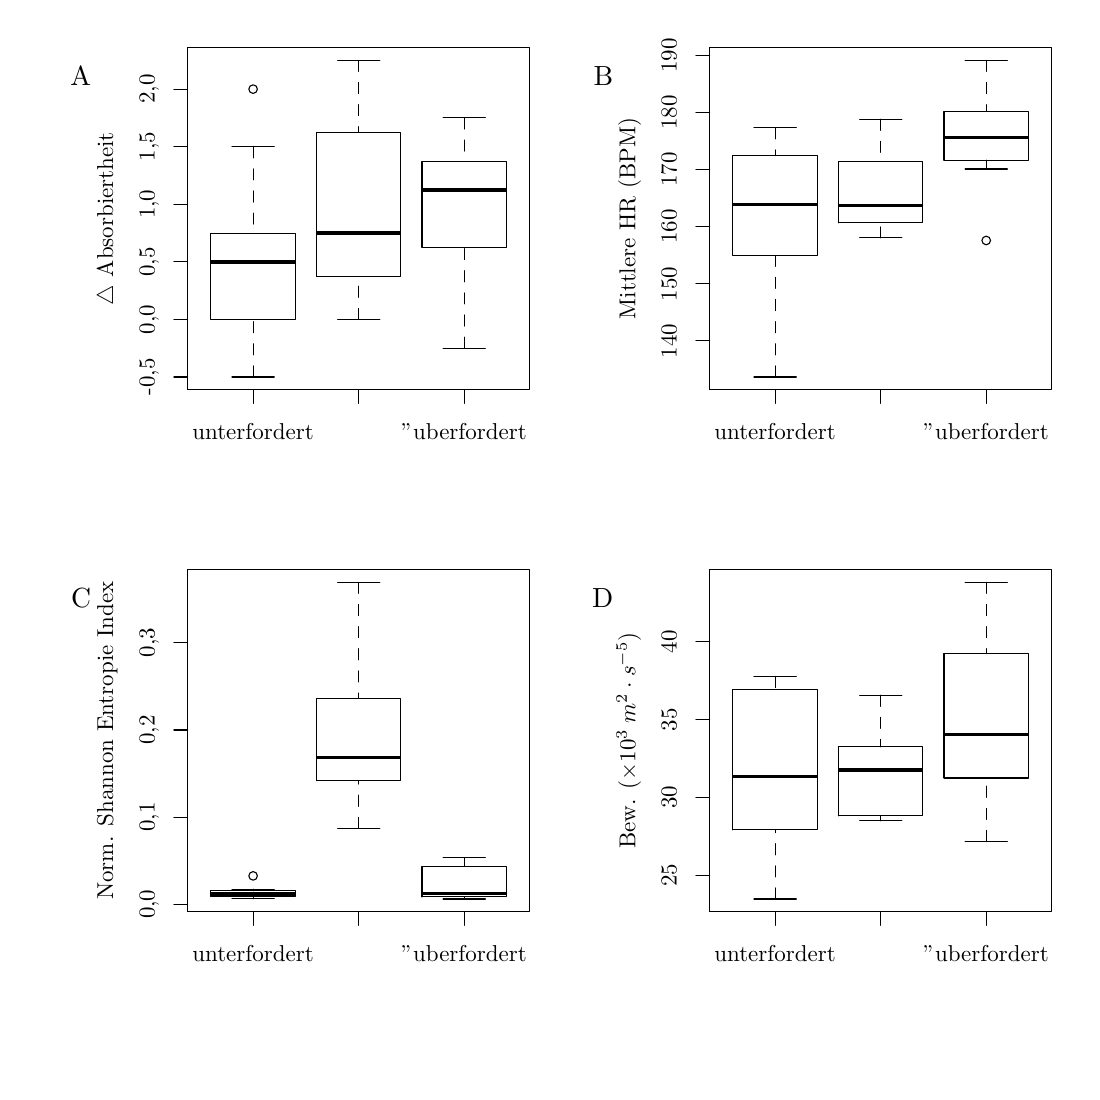
\begin{tikzpicture}[x=1pt,y=1pt]
\definecolor{fillColor}{RGB}{255,255,255}
\path[use as bounding box,fill=fillColor,fill opacity=0.00] (0,0) rectangle (377.25,377.25);
\begin{scope}
\path[clip] ( 57.82,246.44) rectangle (181.40,370.02);
\definecolor{drawColor}{RGB}{0,0,0}

\path[draw=drawColor,line width= 1.2pt,line join=round] ( 66.21,292.63) -- ( 96.72,292.63);

\path[draw=drawColor,line width= 0.4pt,dash pattern=on 4pt off 4pt ,line join=round,line cap=round] ( 81.46,251.02) -- ( 81.46,271.82);

\path[draw=drawColor,line width= 0.4pt,dash pattern=on 4pt off 4pt ,line join=round,line cap=round] ( 81.46,334.24) -- ( 81.46,303.03);

\path[draw=drawColor,line width= 0.4pt,line join=round,line cap=round] ( 73.84,251.02) -- ( 89.09,251.02);

\path[draw=drawColor,line width= 0.4pt,line join=round,line cap=round] ( 73.84,334.24) -- ( 89.09,334.24);

\path[draw=drawColor,line width= 0.4pt,line join=round,line cap=round] ( 66.21,271.82) --
	( 96.72,271.82) --
	( 96.72,303.03) --
	( 66.21,303.03) --
	( 66.21,271.82);

\path[draw=drawColor,line width= 0.4pt,line join=round,line cap=round] ( 81.46,355.04) circle (  1.55);

\path[draw=drawColor,line width= 1.2pt,line join=round] (104.35,303.03) -- (134.86,303.03);

\path[draw=drawColor,line width= 0.4pt,dash pattern=on 4pt off 4pt ,line join=round,line cap=round] (119.61,271.82) -- (119.61,287.43);

\path[draw=drawColor,line width= 0.4pt,dash pattern=on 4pt off 4pt ,line join=round,line cap=round] (119.61,365.45) -- (119.61,339.44);

\path[draw=drawColor,line width= 0.4pt,line join=round,line cap=round] (111.98,271.82) -- (127.24,271.82);

\path[draw=drawColor,line width= 0.4pt,line join=round,line cap=round] (111.98,365.45) -- (127.24,365.45);

\path[draw=drawColor,line width= 0.4pt,line join=round,line cap=round] (104.35,287.43) --
	(134.86,287.43) --
	(134.86,339.44) --
	(104.35,339.44) --
	(104.35,287.43);

\path[draw=drawColor,line width= 1.2pt,line join=round] (142.49,318.63) -- (173.01,318.63);

\path[draw=drawColor,line width= 0.4pt,dash pattern=on 4pt off 4pt ,line join=round,line cap=round] (157.75,261.42) -- (157.75,297.83);

\path[draw=drawColor,line width= 0.4pt,dash pattern=on 4pt off 4pt ,line join=round,line cap=round] (157.75,344.64) -- (157.75,329.04);

\path[draw=drawColor,line width= 0.4pt,line join=round,line cap=round] (150.12,261.42) -- (165.38,261.42);

\path[draw=drawColor,line width= 0.4pt,line join=round,line cap=round] (150.12,344.64) -- (165.38,344.64);

\path[draw=drawColor,line width= 0.4pt,line join=round,line cap=round] (142.49,297.83) --
	(173.01,297.83) --
	(173.01,329.04) --
	(142.49,329.04) --
	(142.49,297.83);
\end{scope}
\begin{scope}
\path[clip] (  0.00,  0.00) rectangle (377.25,377.25);
\definecolor{drawColor}{RGB}{0,0,0}

\path[draw=drawColor,line width= 0.4pt,line join=round,line cap=round] ( 81.46,246.44) -- (157.75,246.44);

\path[draw=drawColor,line width= 0.4pt,line join=round,line cap=round] ( 81.46,246.44) -- ( 81.46,241.46);

\path[draw=drawColor,line width= 0.4pt,line join=round,line cap=round] (119.61,246.44) -- (119.61,241.46);

\path[draw=drawColor,line width= 0.4pt,line join=round,line cap=round] (157.75,246.44) -- (157.75,241.46);

\node[text=drawColor,anchor=base,inner sep=0pt, outer sep=0pt, scale=  0.83] at ( 81.46,228.51) {unterfordert};

\node[text=drawColor,anchor=base,inner sep=0pt, outer sep=0pt, scale=  0.83] at (157.75,228.51) {"uberfordert};

\path[draw=drawColor,line width= 0.4pt,line join=round,line cap=round] ( 57.82,251.02) -- ( 57.82,355.04);

\path[draw=drawColor,line width= 0.4pt,line join=round,line cap=round] ( 57.82,251.02) -- ( 52.84,251.02);

\path[draw=drawColor,line width= 0.4pt,line join=round,line cap=round] ( 57.82,271.82) -- ( 52.84,271.82);

\path[draw=drawColor,line width= 0.4pt,line join=round,line cap=round] ( 57.82,292.63) -- ( 52.84,292.63);

\path[draw=drawColor,line width= 0.4pt,line join=round,line cap=round] ( 57.82,313.43) -- ( 52.84,313.43);

\path[draw=drawColor,line width= 0.4pt,line join=round,line cap=round] ( 57.82,334.24) -- ( 52.84,334.24);

\path[draw=drawColor,line width= 0.4pt,line join=round,line cap=round] ( 57.82,355.04) -- ( 52.84,355.04);

\node[text=drawColor,rotate= 90.00,anchor=base,inner sep=0pt, outer sep=0pt, scale=  0.83] at ( 45.86,251.02) {-0,5};

\node[text=drawColor,rotate= 90.00,anchor=base,inner sep=0pt, outer sep=0pt, scale=  0.83] at ( 45.86,271.82) {0,0};

\node[text=drawColor,rotate= 90.00,anchor=base,inner sep=0pt, outer sep=0pt, scale=  0.83] at ( 45.86,292.63) {0,5};

\node[text=drawColor,rotate= 90.00,anchor=base,inner sep=0pt, outer sep=0pt, scale=  0.83] at ( 45.86,313.43) {1,0};

\node[text=drawColor,rotate= 90.00,anchor=base,inner sep=0pt, outer sep=0pt, scale=  0.83] at ( 45.86,334.24) {1,5};

\node[text=drawColor,rotate= 90.00,anchor=base,inner sep=0pt, outer sep=0pt, scale=  0.83] at ( 45.86,355.04) {2,0};
\end{scope}
\begin{scope}
\path[clip] (  0.00,188.62) rectangle (188.62,377.25);
\definecolor{drawColor}{RGB}{0,0,0}

\node[text=drawColor,rotate= 90.00,anchor=base,inner sep=0pt, outer sep=0pt, scale=  0.83] at ( 30.92,308.23) {$\bigtriangleup$ Absorbiertheit};
\end{scope}
\begin{scope}
\path[clip] (  0.00,  0.00) rectangle (377.25,377.25);
\definecolor{drawColor}{RGB}{0,0,0}

\path[draw=drawColor,line width= 0.4pt,line join=round,line cap=round] ( 57.82,246.44) --
	(181.40,246.44) --
	(181.40,370.02) --
	( 57.82,370.02) --
	( 57.82,246.44);

\node[text=drawColor,anchor=base east,inner sep=0pt, outer sep=0pt, scale=  1.00] at ( 22.96,356.44) {A};
\end{scope}
\begin{scope}
\path[clip] (246.44,246.44) rectangle (370.02,370.02);
\definecolor{drawColor}{RGB}{0,0,0}

\path[draw=drawColor,line width= 1.2pt,line join=round] (254.83,313.25) -- (285.35,313.25);

\path[draw=drawColor,line width= 0.4pt,dash pattern=on 4pt off 4pt ,line join=round,line cap=round] (270.09,251.02) -- (270.09,294.96);

\path[draw=drawColor,line width= 0.4pt,dash pattern=on 4pt off 4pt ,line join=round,line cap=round] (270.09,341.04) -- (270.09,331.00);

\path[draw=drawColor,line width= 0.4pt,line join=round,line cap=round] (262.46,251.02) -- (277.72,251.02);

\path[draw=drawColor,line width= 0.4pt,line join=round,line cap=round] (262.46,341.04) -- (277.72,341.04);

\path[draw=drawColor,line width= 0.4pt,line join=round,line cap=round] (254.83,294.96) --
	(285.35,294.96) --
	(285.35,331.00) --
	(254.83,331.00) --
	(254.83,294.96);

\path[draw=drawColor,line width= 1.2pt,line join=round] (292.97,313.10) -- (323.49,313.10);

\path[draw=drawColor,line width= 0.4pt,dash pattern=on 4pt off 4pt ,line join=round,line cap=round] (308.23,301.29) -- (308.23,306.72);

\path[draw=drawColor,line width= 0.4pt,dash pattern=on 4pt off 4pt ,line join=round,line cap=round] (308.23,344.17) -- (308.23,328.92);

\path[draw=drawColor,line width= 0.4pt,line join=round,line cap=round] (300.60,301.29) -- (315.86,301.29);

\path[draw=drawColor,line width= 0.4pt,line join=round,line cap=round] (300.60,344.17) -- (315.86,344.17);

\path[draw=drawColor,line width= 0.4pt,line join=round,line cap=round] (292.97,306.72) --
	(323.49,306.72) --
	(323.49,328.92) --
	(292.97,328.92) --
	(292.97,306.72);

\path[draw=drawColor,line width= 1.2pt,line join=round] (331.12,337.59) -- (361.63,337.59);

\path[draw=drawColor,line width= 0.4pt,dash pattern=on 4pt off 4pt ,line join=round,line cap=round] (346.37,326.16) -- (346.37,329.34);

\path[draw=drawColor,line width= 0.4pt,dash pattern=on 4pt off 4pt ,line join=round,line cap=round] (346.37,365.45) -- (346.37,346.95);

\path[draw=drawColor,line width= 0.4pt,line join=round,line cap=round] (338.75,326.16) -- (354.00,326.16);

\path[draw=drawColor,line width= 0.4pt,line join=round,line cap=round] (338.75,365.45) -- (354.00,365.45);

\path[draw=drawColor,line width= 0.4pt,line join=round,line cap=round] (331.12,329.34) --
	(361.63,329.34) --
	(361.63,346.95) --
	(331.12,346.95) --
	(331.12,329.34);

\path[draw=drawColor,line width= 0.4pt,line join=round,line cap=round] (346.37,300.35) circle (  1.55);
\end{scope}
\begin{scope}
\path[clip] (  0.00,  0.00) rectangle (377.25,377.25);
\definecolor{drawColor}{RGB}{0,0,0}

\path[draw=drawColor,line width= 0.4pt,line join=round,line cap=round] (270.09,246.44) -- (346.37,246.44);

\path[draw=drawColor,line width= 0.4pt,line join=round,line cap=round] (270.09,246.44) -- (270.09,241.46);

\path[draw=drawColor,line width= 0.4pt,line join=round,line cap=round] (308.23,246.44) -- (308.23,241.46);

\path[draw=drawColor,line width= 0.4pt,line join=round,line cap=round] (346.37,246.44) -- (346.37,241.46);

\node[text=drawColor,anchor=base,inner sep=0pt, outer sep=0pt, scale=  0.83] at (270.09,228.51) {unterfordert};

\node[text=drawColor,anchor=base,inner sep=0pt, outer sep=0pt, scale=  0.83] at (346.37,228.51) {"uberfordert};

\path[draw=drawColor,line width= 0.4pt,line join=round,line cap=round] (246.44,264.07) -- (246.44,367.18);

\path[draw=drawColor,line width= 0.4pt,line join=round,line cap=round] (246.44,264.07) -- (241.46,264.07);

\path[draw=drawColor,line width= 0.4pt,line join=round,line cap=round] (246.44,284.69) -- (241.46,284.69);

\path[draw=drawColor,line width= 0.4pt,line join=round,line cap=round] (246.44,305.32) -- (241.46,305.32);

\path[draw=drawColor,line width= 0.4pt,line join=round,line cap=round] (246.44,325.94) -- (241.46,325.94);

\path[draw=drawColor,line width= 0.4pt,line join=round,line cap=round] (246.44,346.56) -- (241.46,346.56);

\path[draw=drawColor,line width= 0.4pt,line join=round,line cap=round] (246.44,367.18) -- (241.46,367.18);

\node[text=drawColor,rotate= 90.00,anchor=base,inner sep=0pt, outer sep=0pt, scale=  0.83] at (234.49,264.07) {140};

\node[text=drawColor,rotate= 90.00,anchor=base,inner sep=0pt, outer sep=0pt, scale=  0.83] at (234.49,284.69) {150};

\node[text=drawColor,rotate= 90.00,anchor=base,inner sep=0pt, outer sep=0pt, scale=  0.83] at (234.49,305.32) {160};

\node[text=drawColor,rotate= 90.00,anchor=base,inner sep=0pt, outer sep=0pt, scale=  0.83] at (234.49,325.94) {170};

\node[text=drawColor,rotate= 90.00,anchor=base,inner sep=0pt, outer sep=0pt, scale=  0.83] at (234.49,346.56) {180};

\node[text=drawColor,rotate= 90.00,anchor=base,inner sep=0pt, outer sep=0pt, scale=  0.83] at (234.49,367.18) {190};
\end{scope}
\begin{scope}
\path[clip] (188.62,188.62) rectangle (377.25,377.25);
\definecolor{drawColor}{RGB}{0,0,0}

\node[text=drawColor,rotate= 90.00,anchor=base,inner sep=0pt, outer sep=0pt, scale=  0.83] at (219.55,308.23) {Mittlere HR (BPM)};
\end{scope}
\begin{scope}
\path[clip] (  0.00,  0.00) rectangle (377.25,377.25);
\definecolor{drawColor}{RGB}{0,0,0}

\path[draw=drawColor,line width= 0.4pt,line join=round,line cap=round] (246.44,246.44) --
	(370.02,246.44) --
	(370.02,370.02) --
	(246.44,370.02) --
	(246.44,246.44);

\node[text=drawColor,anchor=base east,inner sep=0pt, outer sep=0pt, scale=  1.00] at (211.58,356.44) {B};
\end{scope}
\begin{scope}
\path[clip] ( 57.82, 57.82) rectangle (181.40,181.40);
\definecolor{drawColor}{RGB}{0,0,0}

\path[draw=drawColor,line width= 1.2pt,line join=round] ( 66.21, 64.22) -- ( 96.72, 64.22);

\path[draw=drawColor,line width= 0.4pt,dash pattern=on 4pt off 4pt ,line join=round,line cap=round] ( 81.46, 62.50) -- ( 81.46, 63.38);

\path[draw=drawColor,line width= 0.4pt,dash pattern=on 4pt off 4pt ,line join=round,line cap=round] ( 81.46, 65.91) -- ( 81.46, 65.36);

\path[draw=drawColor,line width= 0.4pt,line join=round,line cap=round] ( 73.84, 62.50) -- ( 89.09, 62.50);

\path[draw=drawColor,line width= 0.4pt,line join=round,line cap=round] ( 73.84, 65.91) -- ( 89.09, 65.91);

\path[draw=drawColor,line width= 0.4pt,line join=round,line cap=round] ( 66.21, 63.38) --
	( 96.72, 63.38) --
	( 96.72, 65.36) --
	( 66.21, 65.36) --
	( 66.21, 63.38);

\path[draw=drawColor,line width= 0.4pt,line join=round,line cap=round] ( 81.46, 70.75) circle (  1.55);

\path[draw=drawColor,line width= 1.2pt,line join=round] (104.35,113.43) -- (134.86,113.43);

\path[draw=drawColor,line width= 0.4pt,dash pattern=on 4pt off 4pt ,line join=round,line cap=round] (119.61, 87.91) -- (119.61,105.14);

\path[draw=drawColor,line width= 0.4pt,dash pattern=on 4pt off 4pt ,line join=round,line cap=round] (119.61,176.82) -- (119.61,134.89);

\path[draw=drawColor,line width= 0.4pt,line join=round,line cap=round] (111.98, 87.91) -- (127.24, 87.91);

\path[draw=drawColor,line width= 0.4pt,line join=round,line cap=round] (111.98,176.82) -- (127.24,176.82);

\path[draw=drawColor,line width= 0.4pt,line join=round,line cap=round] (104.35,105.14) --
	(134.86,105.14) --
	(134.86,134.89) --
	(104.35,134.89) --
	(104.35,105.14);

\path[draw=drawColor,line width= 1.2pt,line join=round] (142.49, 64.30) -- (173.01, 64.30);

\path[draw=drawColor,line width= 0.4pt,dash pattern=on 4pt off 4pt ,line join=round,line cap=round] (157.75, 62.39) -- (157.75, 63.15);

\path[draw=drawColor,line width= 0.4pt,dash pattern=on 4pt off 4pt ,line join=round,line cap=round] (157.75, 77.30) -- (157.75, 74.20);

\path[draw=drawColor,line width= 0.4pt,line join=round,line cap=round] (150.12, 62.39) -- (165.38, 62.39);

\path[draw=drawColor,line width= 0.4pt,line join=round,line cap=round] (150.12, 77.30) -- (165.38, 77.30);

\path[draw=drawColor,line width= 0.4pt,line join=round,line cap=round] (142.49, 63.15) --
	(173.01, 63.15) --
	(173.01, 74.20) --
	(142.49, 74.20) --
	(142.49, 63.15);
\end{scope}
\begin{scope}
\path[clip] (  0.00,  0.00) rectangle (377.25,377.25);
\definecolor{drawColor}{RGB}{0,0,0}

\path[draw=drawColor,line width= 0.4pt,line join=round,line cap=round] ( 81.46, 57.82) -- (157.75, 57.82);

\path[draw=drawColor,line width= 0.4pt,line join=round,line cap=round] ( 81.46, 57.82) -- ( 81.46, 52.84);

\path[draw=drawColor,line width= 0.4pt,line join=round,line cap=round] (119.61, 57.82) -- (119.61, 52.84);

\path[draw=drawColor,line width= 0.4pt,line join=round,line cap=round] (157.75, 57.82) -- (157.75, 52.84);

\node[text=drawColor,anchor=base,inner sep=0pt, outer sep=0pt, scale=  0.83] at ( 81.46, 39.89) {unterfordert};

\node[text=drawColor,anchor=base,inner sep=0pt, outer sep=0pt, scale=  0.83] at (157.75, 39.89) {"uberfordert};

\path[draw=drawColor,line width= 0.4pt,line join=round,line cap=round] ( 57.82, 60.49) -- ( 57.82,154.98);

\path[draw=drawColor,line width= 0.4pt,line join=round,line cap=round] ( 57.82, 60.49) -- ( 52.84, 60.49);

\path[draw=drawColor,line width= 0.4pt,line join=round,line cap=round] ( 57.82, 91.99) -- ( 52.84, 91.99);

\path[draw=drawColor,line width= 0.4pt,line join=round,line cap=round] ( 57.82,123.48) -- ( 52.84,123.48);

\path[draw=drawColor,line width= 0.4pt,line join=round,line cap=round] ( 57.82,154.98) -- ( 52.84,154.98);

\node[text=drawColor,rotate= 90.00,anchor=base,inner sep=0pt, outer sep=0pt, scale=  0.83] at ( 45.86, 60.49) {0,0};

\node[text=drawColor,rotate= 90.00,anchor=base,inner sep=0pt, outer sep=0pt, scale=  0.83] at ( 45.86, 91.99) {0,1};

\node[text=drawColor,rotate= 90.00,anchor=base,inner sep=0pt, outer sep=0pt, scale=  0.83] at ( 45.86,123.48) {0,2};

\node[text=drawColor,rotate= 90.00,anchor=base,inner sep=0pt, outer sep=0pt, scale=  0.83] at ( 45.86,154.98) {0,3};
\end{scope}
\begin{scope}
\path[clip] (  0.00,  0.00) rectangle (188.62,188.62);
\definecolor{drawColor}{RGB}{0,0,0}

\node[text=drawColor,rotate= 90.00,anchor=base,inner sep=0pt, outer sep=0pt, scale=  0.83] at ( 30.92,119.61) {Norm. Shannon Entropie Index};
\end{scope}
\begin{scope}
\path[clip] (  0.00,  0.00) rectangle (377.25,377.25);
\definecolor{drawColor}{RGB}{0,0,0}

\path[draw=drawColor,line width= 0.4pt,line join=round,line cap=round] ( 57.82, 57.82) --
	(181.40, 57.82) --
	(181.40,181.40) --
	( 57.82,181.40) --
	( 57.82, 57.82);

\node[text=drawColor,anchor=base east,inner sep=0pt, outer sep=0pt, scale=  1.00] at ( 22.96,167.82) {C};
\end{scope}
\begin{scope}
\path[clip] (246.44, 57.82) rectangle (370.02,181.40);
\definecolor{drawColor}{RGB}{0,0,0}

\path[draw=drawColor,line width= 1.2pt,line join=round] (254.83,106.72) -- (285.35,106.72);

\path[draw=drawColor,line width= 0.4pt,dash pattern=on 4pt off 4pt ,line join=round,line cap=round] (270.09, 62.39) -- (270.09, 87.39);

\path[draw=drawColor,line width= 0.4pt,dash pattern=on 4pt off 4pt ,line join=round,line cap=round] (270.09,142.78) -- (270.09,138.16);

\path[draw=drawColor,line width= 0.4pt,line join=round,line cap=round] (262.46, 62.39) -- (277.72, 62.39);

\path[draw=drawColor,line width= 0.4pt,line join=round,line cap=round] (262.46,142.78) -- (277.72,142.78);

\path[draw=drawColor,line width= 0.4pt,line join=round,line cap=round] (254.83, 87.39) --
	(285.35, 87.39) --
	(285.35,138.16) --
	(254.83,138.16) --
	(254.83, 87.39);

\path[draw=drawColor,line width= 1.2pt,line join=round] (292.97,108.97) -- (323.49,108.97);

\path[draw=drawColor,line width= 0.4pt,dash pattern=on 4pt off 4pt ,line join=round,line cap=round] (308.23, 90.66) -- (308.23, 92.44);

\path[draw=drawColor,line width= 0.4pt,dash pattern=on 4pt off 4pt ,line join=round,line cap=round] (308.23,136.05) -- (308.23,117.37);

\path[draw=drawColor,line width= 0.4pt,line join=round,line cap=round] (300.60, 90.66) -- (315.86, 90.66);

\path[draw=drawColor,line width= 0.4pt,line join=round,line cap=round] (300.60,136.05) -- (315.86,136.05);

\path[draw=drawColor,line width= 0.4pt,line join=round,line cap=round] (292.97, 92.44) --
	(323.49, 92.44) --
	(323.49,117.37) --
	(292.97,117.37) --
	(292.97, 92.44);

\path[draw=drawColor,line width= 1.2pt,line join=round] (331.12,121.94) -- (361.63,121.94);

\path[draw=drawColor,line width= 0.4pt,dash pattern=on 4pt off 4pt ,line join=round,line cap=round] (346.37, 83.14) -- (346.37,106.13);

\path[draw=drawColor,line width= 0.4pt,dash pattern=on 4pt off 4pt ,line join=round,line cap=round] (346.37,176.82) -- (346.37,151.09);

\path[draw=drawColor,line width= 0.4pt,line join=round,line cap=round] (338.75, 83.14) -- (354.00, 83.14);

\path[draw=drawColor,line width= 0.4pt,line join=round,line cap=round] (338.75,176.82) -- (354.00,176.82);

\path[draw=drawColor,line width= 0.4pt,line join=round,line cap=round] (331.12,106.13) --
	(361.63,106.13) --
	(361.63,151.09) --
	(331.12,151.09) --
	(331.12,106.13);
\end{scope}
\begin{scope}
\path[clip] (  0.00,  0.00) rectangle (377.25,377.25);
\definecolor{drawColor}{RGB}{0,0,0}

\path[draw=drawColor,line width= 0.4pt,line join=round,line cap=round] (270.09, 57.82) -- (346.37, 57.82);

\path[draw=drawColor,line width= 0.4pt,line join=round,line cap=round] (270.09, 57.82) -- (270.09, 52.84);

\path[draw=drawColor,line width= 0.4pt,line join=round,line cap=round] (308.23, 57.82) -- (308.23, 52.84);

\path[draw=drawColor,line width= 0.4pt,line join=round,line cap=round] (346.37, 57.82) -- (346.37, 52.84);

\node[text=drawColor,anchor=base,inner sep=0pt, outer sep=0pt, scale=  0.83] at (270.09, 39.89) {unterfordert};

\node[text=drawColor,anchor=base,inner sep=0pt, outer sep=0pt, scale=  0.83] at (346.37, 39.89) {"uberfordert};

\path[draw=drawColor,line width= 0.4pt,line join=round,line cap=round] (246.44, 71.00) -- (246.44,155.29);

\path[draw=drawColor,line width= 0.4pt,line join=round,line cap=round] (246.44, 71.00) -- (241.46, 71.00);

\path[draw=drawColor,line width= 0.4pt,line join=round,line cap=round] (246.44, 99.10) -- (241.46, 99.10);

\path[draw=drawColor,line width= 0.4pt,line join=round,line cap=round] (246.44,127.20) -- (241.46,127.20);

\path[draw=drawColor,line width= 0.4pt,line join=round,line cap=round] (246.44,155.29) -- (241.46,155.29);

\node[text=drawColor,rotate= 90.00,anchor=base,inner sep=0pt, outer sep=0pt, scale=  0.83] at (234.49, 71.00) {25};

\node[text=drawColor,rotate= 90.00,anchor=base,inner sep=0pt, outer sep=0pt, scale=  0.83] at (234.49, 99.10) {30};

\node[text=drawColor,rotate= 90.00,anchor=base,inner sep=0pt, outer sep=0pt, scale=  0.83] at (234.49,127.20) {35};

\node[text=drawColor,rotate= 90.00,anchor=base,inner sep=0pt, outer sep=0pt, scale=  0.83] at (234.49,155.29) {40};
\end{scope}
\begin{scope}
\path[clip] (188.62,  0.00) rectangle (377.25,188.62);
\definecolor{drawColor}{RGB}{0,0,0}

\node[text=drawColor,rotate= 90.00,anchor=base,inner sep=0pt, outer sep=0pt, scale=  0.83] at (219.55,119.61) {Bew. ($\times 10^3 \: m^2 \cdot s^{-5}$)};
\end{scope}
\begin{scope}
\path[clip] (  0.00,  0.00) rectangle (377.25,377.25);
\definecolor{drawColor}{RGB}{0,0,0}

\path[draw=drawColor,line width= 0.4pt,line join=round,line cap=round] (246.44, 57.82) --
	(370.02, 57.82) --
	(370.02,181.40) --
	(246.44,181.40) --
	(246.44, 57.82);

\node[text=drawColor,anchor=base east,inner sep=0pt, outer sep=0pt, scale=  1.00] at (211.58,167.82) {D};
\end{scope}
\end{tikzpicture}

	\caption[Mittelwertvergleich (Studie: Laufen)]{Mittelwertvergleich der finalen Studie zum Flow-Erleben beim Laufen -- unterfordert, optimal, überfordert. (A) $\bigtriangleup$Absorbiertheit; (B) Mittlere HR; (C) Mittlerer normalisierter Shannon Entropie Index; (D) Bewegungsaufwand. Quelle: Eigene Darstellung \\ \hspace{\textwidth}\emph{Anmerkung}: Bew. = Bewegungsaufwand\\ \hspace{\textwidth}$\bigtriangleup$ Wert berechnet durch die Subtraktion des Baseline-Wertes.}
	\label{fig:5_20_mittelwert_vergleich}
\end{figure}

Ich hinterfrage die Zusammenstellung der Untersuchungspersonen grundsätzlich, da die Gruppe überwiegend aus Fußballern bestand. Mehrere Teilnehmer konnten keine kardio-lokomotorischen Phasensynchronisation herstellen, die die Untersuchungsperson aus der ersten Fallstudie weniger oder mehr in sechs von sechs Sitzungen herstellen konnte. Das begründe ich durch die sporadische Lauferfahrung von Fußballern. Darum fand ich keinen interindividuellen quadratischen Zusammenhang in Form einer umgedrehten U-Kurve wie in Abschnitt~\ref{sub:diskussion_1} und Abschnitt~\ref{sub:diskussion_2} zwischen kardio-lokomotorischen Phasensynchronisation und mittlerer \ac{HR}.

Allgemein zeigt die Operationalisierung durch die \ac{FKS} große Mängel beim Faktor Absorbiertheit in meiner Studie, da das Item "`Ich fühle mich optimal beansprucht."' positiver bewertet wurde als die anderen drei Items des Faktors. Das probeweise Weglassen des Items ergab aber keine Verbesserung der Ergebnisse. \citet{Henk2014} erhielt in seiner Studie vergleichbare Ergebnisse bei der Operationalisierung des Flow-Erlebens durch strukturierte Interviews und der \ac{FKS}. Nichtsdestotrotz halte ich die \ac{FKS} nicht für ein geeignetes Instrument für die Operationalisierung des Flow-Erlebens beim Laufen, da Untersuchungspersonen die Aussagen missverstehen oder individuell interpretieren können. Es bleibt unklar, wie die Antwort in Form eines Kreuzes an einer Stelle der Skala zustande kommt. Die Operationalisierung des Flow-Erlebens durch ein zwar zeitaufwendigeres strukturiertes Interview besitzt bei der korrekten Anwendung einen höheren und präziseren Informationsgehalt über das Flow-Erleben. 

Ich sehe die kardio-lokomotorische Phasensynchronisation und den Bewegungsaufwand aufgrund der Nachbetrachtung als Erfolg versprechende Kandidaten für ein implizites Messverfahren des Flow-Erlebens an. Die kardio-lokomotorische Phasensynchronisation betrachte ich als Voraussetzung für Flow-Erleben und einen personenindividuellen messbaren Unterschied des Bewegungsaufwands ohne eine Laufgeschwindigkeitsänderung als Folge des Flow-Erlebens beim Laufen an. 

\section{Zusammenfassung}
\label{sec:zusammenfassung_5}

Von drei Studien dienten die ersten beiden Fallstudien mit jeweils einer Untersuchungsperson zur Hypothesenbildung und testeten Annahmen für den Einzelfall. In der dritten Studie mit 36 Untersuchungsteilnehmern testete ich die aufgestellten Forschungshypothesen. Die Ergebnisse der drei Studien bestätigen statistisch keine der von mir im Vorfeld getroffenen Annahmen. Dennoch geben sie mir Hinweise auf:

\begin{itemize}
	\item einen personenindividuellen quadratischen Zusammenhang in Form einer umgedrehten U-Kurve zwischen Flow-Erleben und mittlere HR
	\item einen personenindividuellen positiven linearen Zusammenhang zwischen Flow-Erleben und kardio-lokomotorischer Phasensynchronisation
	\item einen personenindividuellen negativen linearen Zusammenhang von Flow-Erleben und Bewegungsaufwand
	\item einen allgemeingültigen positiven linearen Zusammenhang zwischen Flow-Erleben und kardio-lokomotorischer Phasensynchronisation
\end{itemize}

Alle Zusammenhänge benötigen zusätzliche Untersuchungen mit hinreichenden befriedigenden Ergebnissen, bevor einer der Kandidaten als implizites Messverfahren des Flow-Erlebens automatisiert und in Echtzeit mobil von jemandem einzusetzen ist. 